\documentclass[a4paper]{book}
\usepackage{a4wide}
\usepackage{makeidx}
\usepackage{graphicx}
\usepackage{multicol}
\usepackage{float}
\usepackage{listings}
\usepackage{color}
\usepackage{textcomp}
\usepackage{alltt}
\usepackage[utf8]{inputenc}
\usepackage{doxygen}
\lstset{language=C++,inputencoding=utf8,basicstyle=\footnotesize,breaklines=true,breakatwhitespace=true,tabsize=8,numbers=left }
\makeindex
\setcounter{tocdepth}{3}
\renewcommand{\footrulewidth}{0.4pt}
\begin{document}
\begin{titlepage}
\vspace*{7cm}
\begin{center}
{\Large OpenRTM \\[1ex]\large 1.0.0 }\\
\vspace*{1cm}
{\large Generated by Doxygen 1.6.3}\\
\vspace*{0.5cm}
{\small Thu May 24 23:25:21 2012}\\
\end{center}
\end{titlepage}
\clearemptydoublepage
\pagenumbering{roman}
\tableofcontents
\clearemptydoublepage
\pagenumbering{arabic}
\chapter{Namespace Index}
\section{Namespace List}
Here is a list of all namespaces with brief descriptions:\begin{DoxyCompactList}
\item\contentsline{section}{{\bf OpenRTM} }{\pageref{namespaceOpenRTM}}{}
\item\contentsline{section}{{\bf RTC} }{\pageref{namespaceRTC}}{}
\item\contentsline{section}{{\bf RTM} }{\pageref{namespaceRTM}}{}
\item\contentsline{section}{{\bf SDOPackage} }{\pageref{namespaceSDOPackage}}{}
\end{DoxyCompactList}

\chapter{Class Index}
\section{クラス階層}
この継承一覧はおおまかにはソートされていますが、完全にアルファベット順でソートされてはいません。\begin{DoxyCompactList}
\item \contentsline{section}{SDOPackage::AllowedValues}{\pageref{unionSDOPackage_1_1AllowedValues}}{}
\item \contentsline{section}{RTC::ComponentAction}{\pageref{interfaceRTC_1_1ComponentAction}}{}
\begin{DoxyCompactList}
\item \contentsline{section}{RTC::LightweightRTObject}{\pageref{interfaceRTC_1_1LightweightRTObject}}{}
\begin{DoxyCompactList}
\item \contentsline{section}{RTC::DataFlowComponent}{\pageref{interfaceRTC_1_1DataFlowComponent}}{}
\begin{DoxyCompactList}
\item \contentsline{section}{OpenRTM::DataFlowComponent}{\pageref{interfaceOpenRTM_1_1DataFlowComponent}}{}
\end{DoxyCompactList}
\item \contentsline{section}{RTC::Fsm}{\pageref{interfaceRTC_1_1Fsm}}{}
\item \contentsline{section}{RTC::FsmParticipant}{\pageref{interfaceRTC_1_1FsmParticipant}}{}
\item \contentsline{section}{RTC::MultiModeObject}{\pageref{interfaceRTC_1_1MultiModeObject}}{}
\item \contentsline{section}{RTC::RTObject}{\pageref{interfaceRTC_1_1RTObject}}{}
\begin{DoxyCompactList}
\item \contentsline{section}{OpenRTM::DataFlowComponent}{\pageref{interfaceOpenRTM_1_1DataFlowComponent}}{}
\end{DoxyCompactList}
\end{DoxyCompactList}
\end{DoxyCompactList}
\item \contentsline{section}{RTC::ComponentProfile}{\pageref{structRTC_1_1ComponentProfile}}{}
\item \contentsline{section}{SDOPackage::Configuration}{\pageref{interfaceSDOPackage_1_1Configuration}}{}
\item \contentsline{section}{SDOPackage::ConfigurationSet}{\pageref{structSDOPackage_1_1ConfigurationSet}}{}
\item \contentsline{section}{RTC::ConnectorProfile}{\pageref{structRTC_1_1ConnectorProfile}}{}
\item \contentsline{section}{RTC::DataFlowComponentAction}{\pageref{interfaceRTC_1_1DataFlowComponentAction}}{}
\begin{DoxyCompactList}
\item \contentsline{section}{RTC::DataFlowComponent}{\pageref{interfaceRTC_1_1DataFlowComponent}}{}
\end{DoxyCompactList}
\item \contentsline{section}{SDOPackage::DeviceProfile}{\pageref{structSDOPackage_1_1DeviceProfile}}{}
\item \contentsline{section}{SDOPackage::EnumerationType}{\pageref{structSDOPackage_1_1EnumerationType}}{}
\item \contentsline{section}{RTC::ExecutionContext}{\pageref{interfaceRTC_1_1ExecutionContext}}{}
\begin{DoxyCompactList}
\item \contentsline{section}{RTC::ExecutionContextService}{\pageref{interfaceRTC_1_1ExecutionContextService}}{}
\begin{DoxyCompactList}
\item \contentsline{section}{OpenRTM::ExtTrigExecutionContextService}{\pageref{interfaceOpenRTM_1_1ExtTrigExecutionContextService}}{}
\end{DoxyCompactList}
\end{DoxyCompactList}
\item \contentsline{section}{RTC::ExecutionContextProfile}{\pageref{structRTC_1_1ExecutionContextProfile}}{}
\item \contentsline{section}{RTC::FsmBehaviorProfile}{\pageref{structRTC_1_1FsmBehaviorProfile}}{}
\item \contentsline{section}{RTC::FsmObject}{\pageref{interfaceRTC_1_1FsmObject}}{}
\item \contentsline{section}{RTC::FsmParticipantAction}{\pageref{interfaceRTC_1_1FsmParticipantAction}}{}
\begin{DoxyCompactList}
\item \contentsline{section}{RTC::FsmParticipant}{\pageref{interfaceRTC_1_1FsmParticipant}}{}
\end{DoxyCompactList}
\item \contentsline{section}{RTC::FsmProfile}{\pageref{structRTC_1_1FsmProfile}}{}
\item \contentsline{section}{OpenRTM::InPortCdr}{\pageref{interfaceOpenRTM_1_1InPortCdr}}{}
\item \contentsline{section}{SDOPackage::IntervalType}{\pageref{structSDOPackage_1_1IntervalType}}{}
\item \contentsline{section}{RTM::Manager}{\pageref{interfaceRTM_1_1Manager}}{}
\item \contentsline{section}{RTM::ManagerProfile}{\pageref{structRTM_1_1ManagerProfile}}{}
\item \contentsline{section}{RTC::Mode}{\pageref{interfaceRTC_1_1Mode}}{}
\item \contentsline{section}{RTC::ModeCapable}{\pageref{interfaceRTC_1_1ModeCapable}}{}
\begin{DoxyCompactList}
\item \contentsline{section}{RTC::MultiModeObject}{\pageref{interfaceRTC_1_1MultiModeObject}}{}
\end{DoxyCompactList}
\item \contentsline{section}{RTM::ModuleProfile}{\pageref{structRTM_1_1ModuleProfile}}{}
\item \contentsline{section}{SDOPackage::Monitoring}{\pageref{interfaceSDOPackage_1_1Monitoring}}{}
\item \contentsline{section}{RTC::MultiModeComponentAction}{\pageref{interfaceRTC_1_1MultiModeComponentAction}}{}
\begin{DoxyCompactList}
\item \contentsline{section}{RTC::MultiModeObject}{\pageref{interfaceRTC_1_1MultiModeObject}}{}
\end{DoxyCompactList}
\item \contentsline{section}{SDOPackage::NameValue}{\pageref{structSDOPackage_1_1NameValue}}{}
\item \contentsline{section}{SDOPackage::Numeric}{\pageref{unionSDOPackage_1_1Numeric}}{}
\item \contentsline{section}{SDOPackage::Organization}{\pageref{interfaceSDOPackage_1_1Organization}}{}
\item \contentsline{section}{SDOPackage::OrganizationProperty}{\pageref{structSDOPackage_1_1OrganizationProperty}}{}
\item \contentsline{section}{OpenRTM::OutPortCdr}{\pageref{interfaceOpenRTM_1_1OutPortCdr}}{}
\item \contentsline{section}{SDOPackage::Parameter}{\pageref{structSDOPackage_1_1Parameter}}{}
\item \contentsline{section}{RTC::PortInterfaceProfile}{\pageref{structRTC_1_1PortInterfaceProfile}}{}
\item \contentsline{section}{RTC::PortProfile}{\pageref{structRTC_1_1PortProfile}}{}
\item \contentsline{section}{SDOPackage::RangeType}{\pageref{structSDOPackage_1_1RangeType}}{}
\item \contentsline{section}{SDOPackage::SDOService}{\pageref{interfaceSDOPackage_1_1SDOService}}{}
\begin{DoxyCompactList}
\item \contentsline{section}{RTC::ExecutionContextService}{\pageref{interfaceRTC_1_1ExecutionContextService}}{}
\item \contentsline{section}{RTC::FsmService}{\pageref{interfaceRTC_1_1FsmService}}{}
\item \contentsline{section}{RTC::PortService}{\pageref{interfaceRTC_1_1PortService}}{}
\end{DoxyCompactList}
\item \contentsline{section}{SDOPackage::SDOSystemElement}{\pageref{interfaceSDOPackage_1_1SDOSystemElement}}{}
\begin{DoxyCompactList}
\item \contentsline{section}{SDOPackage::SDO}{\pageref{interfaceSDOPackage_1_1SDO}}{}
\begin{DoxyCompactList}
\item \contentsline{section}{RTC::RTObject}{\pageref{interfaceRTC_1_1RTObject}}{}
\end{DoxyCompactList}
\end{DoxyCompactList}
\item \contentsline{section}{SDOPackage::ServiceProfile}{\pageref{structSDOPackage_1_1ServiceProfile}}{}
\item \contentsline{section}{RTC::Time}{\pageref{structRTC_1_1Time}}{}
\item \contentsline{section}{RTC::TimedBoolean}{\pageref{structRTC_1_1TimedBoolean}}{}
\item \contentsline{section}{RTC::TimedBooleanSeq}{\pageref{structRTC_1_1TimedBooleanSeq}}{}
\item \contentsline{section}{RTC::TimedChar}{\pageref{structRTC_1_1TimedChar}}{}
\item \contentsline{section}{RTC::TimedCharSeq}{\pageref{structRTC_1_1TimedCharSeq}}{}
\item \contentsline{section}{RTC::TimedDouble}{\pageref{structRTC_1_1TimedDouble}}{}
\item \contentsline{section}{RTC::TimedDoubleSeq}{\pageref{structRTC_1_1TimedDoubleSeq}}{}
\item \contentsline{section}{RTC::TimedFloat}{\pageref{structRTC_1_1TimedFloat}}{}
\item \contentsline{section}{RTC::TimedFloatSeq}{\pageref{structRTC_1_1TimedFloatSeq}}{}
\item \contentsline{section}{RTC::TimedLong}{\pageref{structRTC_1_1TimedLong}}{}
\item \contentsline{section}{RTC::TimedLongSeq}{\pageref{structRTC_1_1TimedLongSeq}}{}
\item \contentsline{section}{RTC::TimedOctet}{\pageref{structRTC_1_1TimedOctet}}{}
\item \contentsline{section}{RTC::TimedOctetSeq}{\pageref{structRTC_1_1TimedOctetSeq}}{}
\item \contentsline{section}{RTC::TimedShort}{\pageref{structRTC_1_1TimedShort}}{}
\item \contentsline{section}{RTC::TimedShortSeq}{\pageref{structRTC_1_1TimedShortSeq}}{}
\item \contentsline{section}{RTC::TimedState}{\pageref{structRTC_1_1TimedState}}{}
\item \contentsline{section}{RTC::TimedString}{\pageref{structRTC_1_1TimedString}}{}
\item \contentsline{section}{RTC::TimedStringSeq}{\pageref{structRTC_1_1TimedStringSeq}}{}
\item \contentsline{section}{RTC::TimedULong}{\pageref{structRTC_1_1TimedULong}}{}
\item \contentsline{section}{RTC::TimedULongSeq}{\pageref{structRTC_1_1TimedULongSeq}}{}
\item \contentsline{section}{RTC::TimedUShort}{\pageref{structRTC_1_1TimedUShort}}{}
\item \contentsline{section}{RTC::TimedUShortSeq}{\pageref{structRTC_1_1TimedUShortSeq}}{}
\item \contentsline{section}{RTC::TimedWChar}{\pageref{structRTC_1_1TimedWChar}}{}
\item \contentsline{section}{RTC::TimedWCharSeq}{\pageref{structRTC_1_1TimedWCharSeq}}{}
\item \contentsline{section}{RTC::TimedWString}{\pageref{structRTC_1_1TimedWString}}{}
\item \contentsline{section}{RTC::TimedWStringSeq}{\pageref{structRTC_1_1TimedWStringSeq}}{}
\end{DoxyCompactList}

\chapter{Class Index}
\section{構成}
クラス、構造体、共用体、インタフェースの説明です。\begin{DoxyCompactList}
\item\contentsline{section}{{\bf SDOPackage::AllowedValues} }{\pageref{unionSDOPackage_1_1AllowedValues}}{}
\item\contentsline{section}{{\bf RTC::ComponentAction} }{\pageref{interfaceRTC_1_1ComponentAction}}{}
\item\contentsline{section}{{\bf RTC::ComponentProfile} }{\pageref{structRTC_1_1ComponentProfile}}{}
\item\contentsline{section}{{\bf SDOPackage::Configuration} }{\pageref{interfaceSDOPackage_1_1Configuration}}{}
\item\contentsline{section}{{\bf SDOPackage::ConfigurationSet} }{\pageref{structSDOPackage_1_1ConfigurationSet}}{}
\item\contentsline{section}{{\bf RTC::ConnectorProfile} }{\pageref{structRTC_1_1ConnectorProfile}}{}
\item\contentsline{section}{{\bf RTC::DataFlowComponent} }{\pageref{interfaceRTC_1_1DataFlowComponent}}{}
\item\contentsline{section}{{\bf OpenRTM::DataFlowComponent} }{\pageref{interfaceOpenRTM_1_1DataFlowComponent}}{}
\item\contentsline{section}{{\bf RTC::DataFlowComponentAction} }{\pageref{interfaceRTC_1_1DataFlowComponentAction}}{}
\item\contentsline{section}{{\bf SDOPackage::DeviceProfile} }{\pageref{structSDOPackage_1_1DeviceProfile}}{}
\item\contentsline{section}{{\bf SDOPackage::EnumerationType} }{\pageref{structSDOPackage_1_1EnumerationType}}{}
\item\contentsline{section}{{\bf RTC::ExecutionContext} }{\pageref{interfaceRTC_1_1ExecutionContext}}{}
\item\contentsline{section}{{\bf RTC::ExecutionContextProfile} }{\pageref{structRTC_1_1ExecutionContextProfile}}{}
\item\contentsline{section}{{\bf RTC::ExecutionContextService} }{\pageref{interfaceRTC_1_1ExecutionContextService}}{}
\item\contentsline{section}{{\bf OpenRTM::ExtTrigExecutionContextService} }{\pageref{interfaceOpenRTM_1_1ExtTrigExecutionContextService}}{}
\item\contentsline{section}{{\bf RTC::Fsm} }{\pageref{interfaceRTC_1_1Fsm}}{}
\item\contentsline{section}{{\bf RTC::FsmBehaviorProfile} }{\pageref{structRTC_1_1FsmBehaviorProfile}}{}
\item\contentsline{section}{{\bf RTC::FsmObject} }{\pageref{interfaceRTC_1_1FsmObject}}{}
\item\contentsline{section}{{\bf RTC::FsmParticipant} }{\pageref{interfaceRTC_1_1FsmParticipant}}{}
\item\contentsline{section}{{\bf RTC::FsmParticipantAction} }{\pageref{interfaceRTC_1_1FsmParticipantAction}}{}
\item\contentsline{section}{{\bf RTC::FsmProfile} }{\pageref{structRTC_1_1FsmProfile}}{}
\item\contentsline{section}{{\bf RTC::FsmService} }{\pageref{interfaceRTC_1_1FsmService}}{}
\item\contentsline{section}{{\bf OpenRTM::InPortCdr} }{\pageref{interfaceOpenRTM_1_1InPortCdr}}{}
\item\contentsline{section}{{\bf SDOPackage::IntervalType} }{\pageref{structSDOPackage_1_1IntervalType}}{}
\item\contentsline{section}{{\bf RTC::LightweightRTObject} }{\pageref{interfaceRTC_1_1LightweightRTObject}}{}
\item\contentsline{section}{{\bf RTM::Manager} }{\pageref{interfaceRTM_1_1Manager}}{}
\item\contentsline{section}{{\bf RTM::ManagerProfile} }{\pageref{structRTM_1_1ManagerProfile}}{}
\item\contentsline{section}{{\bf RTC::Mode} }{\pageref{interfaceRTC_1_1Mode}}{}
\item\contentsline{section}{{\bf RTC::ModeCapable} }{\pageref{interfaceRTC_1_1ModeCapable}}{}
\item\contentsline{section}{{\bf RTM::ModuleProfile} }{\pageref{structRTM_1_1ModuleProfile}}{}
\item\contentsline{section}{{\bf SDOPackage::Monitoring} }{\pageref{interfaceSDOPackage_1_1Monitoring}}{}
\item\contentsline{section}{{\bf RTC::MultiModeComponentAction} }{\pageref{interfaceRTC_1_1MultiModeComponentAction}}{}
\item\contentsline{section}{{\bf RTC::MultiModeObject} }{\pageref{interfaceRTC_1_1MultiModeObject}}{}
\item\contentsline{section}{{\bf SDOPackage::NameValue} }{\pageref{structSDOPackage_1_1NameValue}}{}
\item\contentsline{section}{{\bf SDOPackage::Numeric} }{\pageref{unionSDOPackage_1_1Numeric}}{}
\item\contentsline{section}{{\bf SDOPackage::Organization} }{\pageref{interfaceSDOPackage_1_1Organization}}{}
\item\contentsline{section}{{\bf SDOPackage::OrganizationProperty} }{\pageref{structSDOPackage_1_1OrganizationProperty}}{}
\item\contentsline{section}{{\bf OpenRTM::OutPortCdr} }{\pageref{interfaceOpenRTM_1_1OutPortCdr}}{}
\item\contentsline{section}{{\bf SDOPackage::Parameter} }{\pageref{structSDOPackage_1_1Parameter}}{}
\item\contentsline{section}{{\bf RTC::PortInterfaceProfile} }{\pageref{structRTC_1_1PortInterfaceProfile}}{}
\item\contentsline{section}{{\bf RTC::PortProfile} }{\pageref{structRTC_1_1PortProfile}}{}
\item\contentsline{section}{{\bf RTC::PortService} }{\pageref{interfaceRTC_1_1PortService}}{}
\item\contentsline{section}{{\bf SDOPackage::RangeType} }{\pageref{structSDOPackage_1_1RangeType}}{}
\item\contentsline{section}{{\bf RTC::RTObject} }{\pageref{interfaceRTC_1_1RTObject}}{}
\item\contentsline{section}{{\bf SDOPackage::SDO} }{\pageref{interfaceSDOPackage_1_1SDO}}{}
\item\contentsline{section}{{\bf SDOPackage::SDOService} }{\pageref{interfaceSDOPackage_1_1SDOService}}{}
\item\contentsline{section}{{\bf SDOPackage::SDOSystemElement} }{\pageref{interfaceSDOPackage_1_1SDOSystemElement}}{}
\item\contentsline{section}{{\bf SDOPackage::ServiceProfile} }{\pageref{structSDOPackage_1_1ServiceProfile}}{}
\item\contentsline{section}{{\bf RTC::Time} }{\pageref{structRTC_1_1Time}}{}
\item\contentsline{section}{{\bf RTC::TimedBoolean} }{\pageref{structRTC_1_1TimedBoolean}}{}
\item\contentsline{section}{{\bf RTC::TimedBooleanSeq} }{\pageref{structRTC_1_1TimedBooleanSeq}}{}
\item\contentsline{section}{{\bf RTC::TimedChar} }{\pageref{structRTC_1_1TimedChar}}{}
\item\contentsline{section}{{\bf RTC::TimedCharSeq} }{\pageref{structRTC_1_1TimedCharSeq}}{}
\item\contentsline{section}{{\bf RTC::TimedDouble} }{\pageref{structRTC_1_1TimedDouble}}{}
\item\contentsline{section}{{\bf RTC::TimedDoubleSeq} }{\pageref{structRTC_1_1TimedDoubleSeq}}{}
\item\contentsline{section}{{\bf RTC::TimedFloat} }{\pageref{structRTC_1_1TimedFloat}}{}
\item\contentsline{section}{{\bf RTC::TimedFloatSeq} }{\pageref{structRTC_1_1TimedFloatSeq}}{}
\item\contentsline{section}{{\bf RTC::TimedLong} }{\pageref{structRTC_1_1TimedLong}}{}
\item\contentsline{section}{{\bf RTC::TimedLongSeq} }{\pageref{structRTC_1_1TimedLongSeq}}{}
\item\contentsline{section}{{\bf RTC::TimedOctet} }{\pageref{structRTC_1_1TimedOctet}}{}
\item\contentsline{section}{{\bf RTC::TimedOctetSeq} }{\pageref{structRTC_1_1TimedOctetSeq}}{}
\item\contentsline{section}{{\bf RTC::TimedShort} }{\pageref{structRTC_1_1TimedShort}}{}
\item\contentsline{section}{{\bf RTC::TimedShortSeq} }{\pageref{structRTC_1_1TimedShortSeq}}{}
\item\contentsline{section}{{\bf RTC::TimedState} }{\pageref{structRTC_1_1TimedState}}{}
\item\contentsline{section}{{\bf RTC::TimedString} }{\pageref{structRTC_1_1TimedString}}{}
\item\contentsline{section}{{\bf RTC::TimedStringSeq} }{\pageref{structRTC_1_1TimedStringSeq}}{}
\item\contentsline{section}{{\bf RTC::TimedULong} }{\pageref{structRTC_1_1TimedULong}}{}
\item\contentsline{section}{{\bf RTC::TimedULongSeq} }{\pageref{structRTC_1_1TimedULongSeq}}{}
\item\contentsline{section}{{\bf RTC::TimedUShort} }{\pageref{structRTC_1_1TimedUShort}}{}
\item\contentsline{section}{{\bf RTC::TimedUShortSeq} }{\pageref{structRTC_1_1TimedUShortSeq}}{}
\item\contentsline{section}{{\bf RTC::TimedWChar} }{\pageref{structRTC_1_1TimedWChar}}{}
\item\contentsline{section}{{\bf RTC::TimedWCharSeq} }{\pageref{structRTC_1_1TimedWCharSeq}}{}
\item\contentsline{section}{{\bf RTC::TimedWString} }{\pageref{structRTC_1_1TimedWString}}{}
\item\contentsline{section}{{\bf RTC::TimedWStringSeq} }{\pageref{structRTC_1_1TimedWStringSeq}}{}
\end{DoxyCompactList}

\chapter{File Index}
\section{ファイル一覧}
これはファイル一覧です。\begin{DoxyCompactList}
\item\contentsline{section}{{\bf BasicDataType.idl} }{\pageref{BasicDataType_8idl}}{}
\item\contentsline{section}{{\bf DataPort.idl} (DataPort interface definition )}{\pageref{DataPort_8idl}}{}
\item\contentsline{section}{{\bf Manager.idl} }{\pageref{Manager_8idl}}{}
\item\contentsline{section}{{\bf OpenRTM.idl} (\doxyref{OpenRTM}{p.}{namespaceOpenRTM} interface definition )}{\pageref{OpenRTM_8idl}}{}
\item\contentsline{section}{{\bf RTC.idl} }{\pageref{RTC_8idl}}{}
\item\contentsline{section}{{\bf SDOPackage.idl} }{\pageref{SDOPackage_8idl}}{}
\end{DoxyCompactList}

\chapter{Namespace Documentation}
\section{coil Namespace Reference}
\label{namespacecoil}\index{coil@{coil}}


Common Object Interface Layer.  


\subsection*{Classes}
\begin{DoxyCompactItemize}
\item 
class {\bf Allocator}
\begin{DoxyCompactList}\small\item\em \doxyref{Allocator}{p.}{classcoil_1_1Allocator} class. \item\end{DoxyCompactList}\item 
class {\bf Async}
\begin{DoxyCompactList}\small\item\em \doxyref{Async}{p.}{classcoil_1_1Async} class. \item\end{DoxyCompactList}\item 
class {\bf Async\_\-t}
\begin{DoxyCompactList}\small\item\em \doxyref{Async\_\-t}{p.}{classcoil_1_1Async__t} template class. \item\end{DoxyCompactList}\item 
class {\bf Async\_\-ref\_\-t}
\begin{DoxyCompactList}\small\item\em \doxyref{Async\_\-ref\_\-t}{p.}{classcoil_1_1Async__ref__t} template class. \item\end{DoxyCompactList}\item 
class {\bf Condition}
\begin{DoxyCompactList}\small\item\em \doxyref{Condition}{p.}{classcoil_1_1Condition} template class. \item\end{DoxyCompactList}\item 
class {\bf DynamicLib}
\begin{DoxyCompactList}\small\item\em \doxyref{DynamicLib}{p.}{classcoil_1_1DynamicLib} class. \item\end{DoxyCompactList}\item 
class {\bf Factory}
\begin{DoxyCompactList}\small\item\em \doxyref{Factory}{p.}{classcoil_1_1Factory} template class. \item\end{DoxyCompactList}\item 
class {\bf GlobalFactory}
\begin{DoxyCompactList}\small\item\em \doxyref{GlobalFactory}{p.}{classcoil_1_1GlobalFactory} template class. \item\end{DoxyCompactList}\item 
class {\bf Guard}
\begin{DoxyCompactList}\small\item\em \doxyref{Guard}{p.}{classcoil_1_1Guard} template class. \item\end{DoxyCompactList}\item 
class {\bf log\_\-streambuf}
\begin{DoxyCompactList}\small\item\em \doxyref{log\_\-streambuf}{p.}{classcoil_1_1log__streambuf} template class \item\end{DoxyCompactList}\item 
class {\bf log\_\-stream}
\begin{DoxyCompactList}\small\item\em \doxyref{log\_\-stream}{p.}{classcoil_1_1log__stream} template class \item\end{DoxyCompactList}\item 
class {\bf Mutex}
\begin{DoxyCompactList}\small\item\em \doxyref{Mutex}{p.}{classcoil_1_1Mutex} class. \item\end{DoxyCompactList}\item 
class {\bf NonCopyable}
\begin{DoxyCompactList}\small\item\em Non-\/copyable Mixin. \item\end{DoxyCompactList}\item 
class {\bf NonCopyableCRTP}
\item 
class {\bf GetOpt}
\begin{DoxyCompactList}\small\item\em \doxyref{GetOpt}{p.}{classcoil_1_1GetOpt} class. \item\end{DoxyCompactList}\item 
class {\bf PeriodicTask}
\begin{DoxyCompactList}\small\item\em \doxyref{PeriodicTask}{p.}{classcoil_1_1PeriodicTask} class. \item\end{DoxyCompactList}\item 
class {\bf TaskFuncBase}
\begin{DoxyCompactList}\small\item\em \doxyref{TaskFuncBase}{p.}{classcoil_1_1TaskFuncBase} class. \item\end{DoxyCompactList}\item 
class {\bf TaskFunc}
\begin{DoxyCompactList}\small\item\em \doxyref{TaskFunc}{p.}{classcoil_1_1TaskFunc} template class. \item\end{DoxyCompactList}\item 
class {\bf PeriodicTaskBase}
\begin{DoxyCompactList}\small\item\em \doxyref{PeriodicTaskBase}{p.}{classcoil_1_1PeriodicTaskBase} class. \item\end{DoxyCompactList}\item 
class {\bf Properties}
\begin{DoxyCompactList}\small\item\em Class represents a set of properties. \item\end{DoxyCompactList}\item 
class {\bf SignalAction}
\begin{DoxyCompactList}\small\item\em \doxyref{SignalAction}{p.}{classcoil_1_1SignalAction} class. \item\end{DoxyCompactList}\item 
class {\bf Singleton}
\begin{DoxyCompactList}\small\item\em \doxyref{Singleton}{p.}{classcoil_1_1Singleton} template class. \item\end{DoxyCompactList}\item 
class {\bf Task}
\begin{DoxyCompactList}\small\item\em \doxyref{Task}{p.}{classcoil_1_1Task} class. \item\end{DoxyCompactList}\item 
class {\bf TimeMeasure}
\begin{DoxyCompactList}\small\item\em \doxyref{TimeMeasure}{p.}{classcoil_1_1TimeMeasure} class. \item\end{DoxyCompactList}\item 
class {\bf Timer}
\begin{DoxyCompactList}\small\item\em \doxyref{Timer}{p.}{classcoil_1_1Timer} class. \item\end{DoxyCompactList}\item 
class {\bf TimeValue}
\begin{DoxyCompactList}\small\item\em \doxyref{TimeValue}{p.}{classcoil_1_1TimeValue} class. \item\end{DoxyCompactList}\item 
class {\bf UUID}
\item 
class {\bf UUID\_\-Generator}
\end{DoxyCompactItemize}
\subsection*{Typedefs}
\begin{DoxyCompactItemize}
\item 
typedef {\bf log\_\-streambuf}$<$ char $>$ {\bf LogStreamBuffer}
\item 
typedef {\bf log\_\-stream}$<$ char $>$ {\bf LogStream}
\item 
typedef ::{\bf utsname} {\bf utsname}
\begin{DoxyCompactList}\small\item\em Get System information. \item\end{DoxyCompactList}\item 
typedef ::{\bf pid\_\-t} {\bf pid\_\-t}
\begin{DoxyCompactList}\small\item\em Get process ID of the caller process. \item\end{DoxyCompactList}\item 
typedef void($\ast$ {\bf SignalHandler} )(int)
\item 
typedef std::vector$<$ std::string $>$ {\bf vstring}
\end{DoxyCompactItemize}
\subsection*{Functions}
\begin{DoxyCompactItemize}
\item 
{\footnotesize template$<$typename Object , typename Func $>$ }\\{\bf Async\_\-t}$<$ Object, Func $>$ $\ast$ {\bf AsyncInvoker} (Object $\ast$obj, Func func, bool auto\_\-delete=false)
\begin{DoxyCompactList}\small\item\em Helper function for async member function summons. \item\end{DoxyCompactList}\item 
{\footnotesize template$<$typename Object , typename Func $>$ }\\{\bf Async\_\-ref\_\-t}$<$ Object, Func $>$ $\ast$ {\bf AsyncInvoker} (Object $\ast$obj, Func $\ast$func, bool auto\_\-delete=false)
\begin{DoxyCompactList}\small\item\em Helper function for async member function summons. \item\end{DoxyCompactList}\item 
unsigned short {\bf crc16} (const char $\ast$str, size\_\-t len)
\item 
unsigned long {\bf crc32} (const char $\ast$str, size\_\-t len)
\begin{DoxyCompactList}\small\item\em CRC-\/32 calculation function. \item\end{DoxyCompactList}\item 
{\footnotesize template$<$class AbstractClass , class ConcreteClass $>$ }\\AbstractClass $\ast$ {\bf Creator} ()
\begin{DoxyCompactList}\small\item\em Creator template. \item\end{DoxyCompactList}\item 
{\footnotesize template$<$class AbstractClass , class ConcreteClass $>$ }\\void {\bf Destructor} (AbstractClass $\ast$\&obj)
\begin{DoxyCompactList}\small\item\em Destructor template. \item\end{DoxyCompactList}\item 
std::string {\bf dirname} (char $\ast$path)
\begin{DoxyCompactList}\small\item\em Get a directory part than a file pass. \item\end{DoxyCompactList}\item 
std::string {\bf basename} (const char $\ast$path)
\begin{DoxyCompactList}\small\item\em Get a file name part than a file pass. \item\end{DoxyCompactList}\item 
{\bf coil::vstring} {\bf filelist} (const char $\ast$path, const char $\ast$glob\_\-str=\char`\"{}\char`\"{})
\begin{DoxyCompactList}\small\item\em Get file list. \item\end{DoxyCompactList}\item 
int {\bf uname} ({\bf utsname} $\ast$name)
\item 
{\bf pid\_\-t} {\bf getpid} ()
\item 
{\bf pid\_\-t} {\bf getppid} ()
\begin{DoxyCompactList}\small\item\em Get process ID of the parent process. \item\end{DoxyCompactList}\item 
char $\ast$ {\bf getenv} (const char $\ast$name)
\begin{DoxyCompactList}\small\item\em Get environment variable. \item\end{DoxyCompactList}\item 
int {\bf launch\_\-shell} (std::string command)
\begin{DoxyCompactList}\small\item\em Launching a process. \item\end{DoxyCompactList}\item 
int {\bf daemon} (int nochdir, int noclose)
\item 
bool {\bf dest\_\-to\_\-endpoint} (std::string dest\_\-addr, std::string \&endpoint)
\begin{DoxyCompactList}\small\item\em Getting network interface name from destination address. \item\end{DoxyCompactList}\item 
bool {\bf find\_\-dest\_\-ifname} (std::string dest\_\-addr, std::string \&dest\_\-if)
\begin{DoxyCompactList}\small\item\em Getting network interface name from destination address. \item\end{DoxyCompactList}\item 
bool {\bf ifname\_\-to\_\-ipaddr} (std::string ifname, std::string \&ipaddr)
\begin{DoxyCompactList}\small\item\em Get IP address from a network interface name. \item\end{DoxyCompactList}\item 
std::wstring {\bf string2wstring} (std::string str)
\begin{DoxyCompactList}\small\item\em string to wstring conversion \item\end{DoxyCompactList}\item 
std::string {\bf wstring2string} (std::wstring wstr)
\begin{DoxyCompactList}\small\item\em wstring to string conversion \item\end{DoxyCompactList}\item 
void {\bf toUpper} (std::string \&str)
\begin{DoxyCompactList}\small\item\em Uppercase String Transformation. \item\end{DoxyCompactList}\item 
void {\bf toLower} (std::string \&str)
\begin{DoxyCompactList}\small\item\em Lowercase String Transformation. \item\end{DoxyCompactList}\item 
int {\bf getlinePortable} (std::istream \&istr, std::string \&line)
\begin{DoxyCompactList}\small\item\em Read a line from input stream. \item\end{DoxyCompactList}\item 
bool {\bf isEscaped} (const std::string \&str, std::string::size\_\-type pos)
\begin{DoxyCompactList}\small\item\em Check whether the character is escaped or not. \item\end{DoxyCompactList}\item 
std::string {\bf escape} (const std::string str)
\begin{DoxyCompactList}\small\item\em Escape string. \item\end{DoxyCompactList}\item 
std::string {\bf unescape} (const std::string str)
\begin{DoxyCompactList}\small\item\em Unescape string. \item\end{DoxyCompactList}\item 
void {\bf eraseBlank} (std::string \&str)
\begin{DoxyCompactList}\small\item\em Erase blank characters of string. \item\end{DoxyCompactList}\item 
void {\bf eraseHeadBlank} (std::string \&str)
\begin{DoxyCompactList}\small\item\em Erase the head blank characters of string. \item\end{DoxyCompactList}\item 
void {\bf eraseTailBlank} (std::string \&str)
\begin{DoxyCompactList}\small\item\em Erase the tail blank characters of string. \item\end{DoxyCompactList}\item 
void {\bf eraseBothEndsBlank} (std::string \&str)
\begin{DoxyCompactList}\small\item\em Erase the head blank and the tail blank characters of string. \item\end{DoxyCompactList}\item 
std::string {\bf normalize} (std::string \&str)
\begin{DoxyCompactList}\small\item\em Erase the head/tail blank and replace upper case to lower case. \item\end{DoxyCompactList}\item 
unsigned int {\bf replaceString} (std::string \&str, const std::string from, const std::string to)
\begin{DoxyCompactList}\small\item\em Replace string. \item\end{DoxyCompactList}\item 
{\bf vstring} {\bf split} (const std::string \&input, const std::string \&delimiter, bool ignore\_\-empty=false)
\begin{DoxyCompactList}\small\item\em Split string by delimiter. \item\end{DoxyCompactList}\item 
bool {\bf toBool} (std::string str, std::string yes, std::string no, bool default\_\-value=true)
\begin{DoxyCompactList}\small\item\em Convert given string into bool value. \item\end{DoxyCompactList}\item 
bool {\bf includes} (const {\bf vstring} \&list, std::string value, bool ignore\_\-case=true)
\begin{DoxyCompactList}\small\item\em Include if a string is included in string list. \item\end{DoxyCompactList}\item 
bool {\bf includes} (const std::string \&list, std::string value, bool ignore\_\-case=true)
\begin{DoxyCompactList}\small\item\em Include if a string is included in string list. \item\end{DoxyCompactList}\item 
bool {\bf isAbsolutePath} (const std::string \&str)
\begin{DoxyCompactList}\small\item\em Investigate whether the given string is absolute path or not. \item\end{DoxyCompactList}\item 
bool {\bf isURL} (const std::string \&str)
\begin{DoxyCompactList}\small\item\em Investigate whether the given string is URL or not. \item\end{DoxyCompactList}\item 
{\footnotesize template$<$class Printable $>$ }\\std::string {\bf otos} (Printable n)
\begin{DoxyCompactList}\small\item\em Convert the given object to std::string. \item\end{DoxyCompactList}\item 
{\footnotesize template$<$typename To $>$ }\\bool {\bf stringTo} (To \&val, const char $\ast$str)
\begin{DoxyCompactList}\small\item\em Convert the given std::string to object. \item\end{DoxyCompactList}\item 
{\footnotesize template$<$$>$ }\\bool {\bf stringTo$<$ std::string $>$} (std::string \&val, const char $\ast$str)
\begin{DoxyCompactList}\small\item\em Convert the given string to std::string. \item\end{DoxyCompactList}\item 
{\bf vstring} {\bf unique\_\-sv} ({\bf vstring} sv)
\begin{DoxyCompactList}\small\item\em Eliminate duplication from the given string list. \item\end{DoxyCompactList}\item 
std::string {\bf flatten} ({\bf vstring} sv)
\begin{DoxyCompactList}\small\item\em Create CSV file from the given string list. \item\end{DoxyCompactList}\item 
char $\ast$$\ast$ {\bf toArgv} (const {\bf vstring} \&args)
\begin{DoxyCompactList}\small\item\em Convert the given string list into the argument list. \item\end{DoxyCompactList}\item 
std::string {\bf sprintf} (char const $\ast$\_\-\_\-restrict fmt,...)
\begin{DoxyCompactList}\small\item\em Convert it into a format given with an argumen. \item\end{DoxyCompactList}\item 
unsigned int {\bf sleep} (unsigned int seconds)
\begin{DoxyCompactList}\small\item\em Stop a processing at specified second time. \item\end{DoxyCompactList}\item 
int {\bf sleep} ({\bf TimeValue} interval)
\begin{DoxyCompactList}\small\item\em Stop a processing at specified second time. \item\end{DoxyCompactList}\item 
int {\bf usleep} (useconds\_\-t usec)
\begin{DoxyCompactList}\small\item\em Stop a processing at specified micro second time. \item\end{DoxyCompactList}\item 
int {\bf gettimeofday} (struct timeval $\ast$tv, struct timezone $\ast$tz)
\begin{DoxyCompactList}\small\item\em Get the time and timezone. \item\end{DoxyCompactList}\item 
{\bf TimeValue} {\bf gettimeofday} ()
\begin{DoxyCompactList}\small\item\em Get the time. \item\end{DoxyCompactList}\item 
int {\bf settimeofday} (const struct timeval $\ast$tv, const struct timezone $\ast$tz)
\begin{DoxyCompactList}\small\item\em Set the time and timezone. \item\end{DoxyCompactList}\end{DoxyCompactItemize}


\subsection{Detailed Description}
Common Object Interface Layer. 

\subsection{Typedef Documentation}
\index{coil@{coil}!LogStream@{LogStream}}
\index{LogStream@{LogStream}!coil@{coil}}
\subsubsection[{LogStream}]{\setlength{\rightskip}{0pt plus 5cm}typedef {\bf log\_\-stream}$<$char$>$ {\bf coil::LogStream}}\label{namespacecoil_a61ed7150f67f7f375e4647b7be48eca7}
\index{coil@{coil}!LogStreamBuffer@{LogStreamBuffer}}
\index{LogStreamBuffer@{LogStreamBuffer}!coil@{coil}}
\subsubsection[{LogStreamBuffer}]{\setlength{\rightskip}{0pt plus 5cm}typedef {\bf log\_\-streambuf}$<$char$>$ {\bf coil::LogStreamBuffer}}\label{namespacecoil_aee9db6758e0fffcb55fc3535842d3e98}
\index{coil@{coil}!pid\_\-t@{pid\_\-t}}
\index{pid\_\-t@{pid\_\-t}!coil@{coil}}
\subsubsection[{pid\_\-t}]{\setlength{\rightskip}{0pt plus 5cm}typedef ::{\bf pid\_\-t} {\bf coil::pid\_\-t}}\label{namespacecoil_a9b4fff7de7d767eb84a2ebef6d35d024}


Get process ID of the caller process. 

Return a process ID of the caller process.

\begin{DoxyReturn}{Returns}
Process ID 
\end{DoxyReturn}
\index{coil@{coil}!SignalHandler@{SignalHandler}}
\index{SignalHandler@{SignalHandler}!coil@{coil}}
\subsubsection[{SignalHandler}]{\setlength{\rightskip}{0pt plus 5cm}typedef void($\ast$ {\bf coil::SignalHandler})(int)}\label{namespacecoil_a3935a219154da03913345ab079b4e791}
\index{coil@{coil}!utsname@{utsname}}
\index{utsname@{utsname}!coil@{coil}}
\subsubsection[{utsname}]{\setlength{\rightskip}{0pt plus 5cm}typedef ::{\bf utsname} {\bf coil::utsname}}\label{namespacecoil_adc6b0c76f612cf80e2df3f37b5ed6f76}


Get System information. 

Return a system information to a structure.


\begin{DoxyParams}{Parameters}
\item[{\em name}]Name of structure\end{DoxyParams}
\begin{DoxyReturn}{Returns}
0: Successful, -\/1: failed 
\end{DoxyReturn}
\index{coil@{coil}!vstring@{vstring}}
\index{vstring@{vstring}!coil@{coil}}
\subsubsection[{vstring}]{\setlength{\rightskip}{0pt plus 5cm}typedef std::vector$<$std::string$>$ {\bf coil::vstring}}\label{namespacecoil_ac44b80f207f9471f2cc10a0e4202f9ea}


\subsection{Function Documentation}
\index{coil@{coil}!AsyncInvoker@{AsyncInvoker}}
\index{AsyncInvoker@{AsyncInvoker}!coil@{coil}}
\subsubsection[{AsyncInvoker}]{\setlength{\rightskip}{0pt plus 5cm}template$<$typename Object , typename Func $>$ {\bf Async\_\-ref\_\-t}$<$Object, Func$>$$\ast$ coil::AsyncInvoker (Object $\ast$ {\em obj}, \/  Func $\ast$ {\em func}, \/  bool {\em auto\_\-delete} = {\ttfamily false})\hspace{0.3cm}{\ttfamily  [inline]}}\label{namespacecoil_a6a774d2568d53f800d0504d64cde1f4d}


Helper function for async member function summons. 

Helper function for async member function summons.


\begin{DoxyParams}{Parameters}
\item[{\em obj}]The target object for the asynchronous function. \item[{\em func}]Asynchronous function. \item[{\em auto\_\-delete}]flag for automatic instance destruction.\end{DoxyParams}
\begin{DoxyReturn}{Returns}
\doxyref{Async\_\-ref\_\-t}{p.}{classcoil_1_1Async__ref__t} Instance 
\end{DoxyReturn}
\index{coil@{coil}!AsyncInvoker@{AsyncInvoker}}
\index{AsyncInvoker@{AsyncInvoker}!coil@{coil}}
\subsubsection[{AsyncInvoker}]{\setlength{\rightskip}{0pt plus 5cm}template$<$typename Object , typename Func $>$ {\bf Async\_\-t}$<$Object, Func$>$$\ast$ coil::AsyncInvoker (Object $\ast$ {\em obj}, \/  Func {\em func}, \/  bool {\em auto\_\-delete} = {\ttfamily false})\hspace{0.3cm}{\ttfamily  [inline]}}\label{namespacecoil_af871c8ea1919908ab5dd7c84897e7b3e}


Helper function for async member function summons. 

Helper function for async member function summons.


\begin{DoxyParams}{Parameters}
\item[{\em obj}]The target object for the asynchronous function. \item[{\em func}]Asynchronous function. \item[{\em auto\_\-delete}]flag for automatic instance destruction.\end{DoxyParams}
\begin{DoxyReturn}{Returns}
\doxyref{Async\_\-t}{p.}{classcoil_1_1Async__t} Instance 
\end{DoxyReturn}
\index{coil@{coil}!basename@{basename}}
\index{basename@{basename}!coil@{coil}}
\subsubsection[{basename}]{\setlength{\rightskip}{0pt plus 5cm}std::string coil::basename (const char $\ast$ {\em path})\hspace{0.3cm}{\ttfamily  [inline]}}\label{namespacecoil_aa32553db1abc9b9c9dfd0a201f69ecf0}


Get a file name part than a file pass. 

Get a directory part than a file pass.


\begin{DoxyParams}{Parameters}
\item[{\em path}]File path\end{DoxyParams}
\begin{DoxyReturn}{Returns}
File name 
\end{DoxyReturn}
\index{coil@{coil}!crc16@{crc16}}
\index{crc16@{crc16}!coil@{coil}}
\subsubsection[{crc16}]{\setlength{\rightskip}{0pt plus 5cm}unsigned short coil::crc16 (const char $\ast$ {\em str}, \/  size\_\-t {\em len})}\label{namespacecoil_a810e5279eee44c4bfd70261cd51dcd8c}
\index{coil@{coil}!crc32@{crc32}}
\index{crc32@{crc32}!coil@{coil}}
\subsubsection[{crc32}]{\setlength{\rightskip}{0pt plus 5cm}unsigned long coil::crc32 (const char $\ast$ {\em str}, \/  size\_\-t {\em len})}\label{namespacecoil_a6c3973b2c232b1b7608ad97cc3de7323}


CRC-\/32 calculation function. 

CRC type: RFC2083 Appendix 15 {\tt http://www.faqs.org/rfcs/rfc2083.html} {\tt http://www.efg2.com/Lab/Mathematics/CRC.htm} CRC polynomial: 0xedb88320L Initial value: 0xFFFFFFFF Output XOR: 0xFFFFFFFF Input bit inversion: None Output bit inversion: None Bit shift: right


\begin{DoxyParams}{Parameters}
\item[{\em str}]Data stream \item[{\em len}]Data length\end{DoxyParams}
\begin{DoxyReturn}{Returns}
Result calculation 
\end{DoxyReturn}
\index{coil@{coil}!Creator@{Creator}}
\index{Creator@{Creator}!coil@{coil}}
\subsubsection[{Creator}]{\setlength{\rightskip}{0pt plus 5cm}template$<$class AbstractClass , class ConcreteClass $>$ AbstractClass$\ast$ coil::Creator ()\hspace{0.3cm}{\ttfamily  [inline]}}\label{namespacecoil_a7f96c97693a425d037804baac00e095a}


Creator template. 

\index{coil@{coil}!daemon@{daemon}}
\index{daemon@{daemon}!coil@{coil}}
\subsubsection[{daemon}]{\setlength{\rightskip}{0pt plus 5cm}int coil::daemon (int {\em nochdir}, \/  int {\em noclose})}\label{namespacecoil_a4cb16acad915bcfb507f9721d811dd06}
\index{coil@{coil}!dest\_\-to\_\-endpoint@{dest\_\-to\_\-endpoint}}
\index{dest\_\-to\_\-endpoint@{dest\_\-to\_\-endpoint}!coil@{coil}}
\subsubsection[{dest\_\-to\_\-endpoint}]{\setlength{\rightskip}{0pt plus 5cm}bool coil::dest\_\-to\_\-endpoint (std::string {\em dest\_\-addr}, \/  std::string \& {\em endpoint})}\label{namespacecoil_a41b12f5eee452f6e0141c03f66d1451e}


Getting network interface name from destination address. 

This operation returns IP address of a endpoint to be used to communicate with the given destination address. IP address and FQDN hostname are available for the destination address dest\_\-addr. If a destination address are reachable and an endpoint IP address is available, this operation returns true, and otherwise false.


\begin{DoxyParams}{Parameters}
\item[{\em dest\_\-addr}]a destination address or host name \item[{\em endpoint}]a IP address of the endpoint to be used to communicate with the destination address \end{DoxyParams}
\begin{DoxyReturn}{Returns}
successful: true, failed: false 
\end{DoxyReturn}
\index{coil@{coil}!Destructor@{Destructor}}
\index{Destructor@{Destructor}!coil@{coil}}
\subsubsection[{Destructor}]{\setlength{\rightskip}{0pt plus 5cm}template$<$class AbstractClass , class ConcreteClass $>$ void coil::Destructor (AbstractClass $\ast$\& {\em obj})\hspace{0.3cm}{\ttfamily  [inline]}}\label{namespacecoil_a3d92b40c32da6da798031e58bb1c2cf0}


Destructor template. 

\index{coil@{coil}!dirname@{dirname}}
\index{dirname@{dirname}!coil@{coil}}
\subsubsection[{dirname}]{\setlength{\rightskip}{0pt plus 5cm}std::string coil::dirname (char $\ast$ {\em path})\hspace{0.3cm}{\ttfamily  [inline]}}\label{namespacecoil_abdcffe47716c2bef3011516e58ae6632}


Get a directory part than a file pass. 

Get a directory part than a file pass.


\begin{DoxyParams}{Parameters}
\item[{\em path}]File path\end{DoxyParams}
\begin{DoxyReturn}{Returns}
Directory name 
\end{DoxyReturn}
\index{coil@{coil}!eraseBlank@{eraseBlank}}
\index{eraseBlank@{eraseBlank}!coil@{coil}}
\subsubsection[{eraseBlank}]{\setlength{\rightskip}{0pt plus 5cm}void coil::eraseBlank (std::string \& {\em str})}\label{namespacecoil_aa9311f7aa6bcc858fca2551b1541c9b5}


Erase blank characters of string. 

Erase blank characters that exist at the head of the given string. Space ' 'and tab '$\backslash$t' are supported as the blank character.


\begin{DoxyParams}{Parameters}
\item[{\em str}]The target blank characters of string for the erase \end{DoxyParams}
\index{coil@{coil}!eraseBothEndsBlank@{eraseBothEndsBlank}}
\index{eraseBothEndsBlank@{eraseBothEndsBlank}!coil@{coil}}
\subsubsection[{eraseBothEndsBlank}]{\setlength{\rightskip}{0pt plus 5cm}void coil::eraseBothEndsBlank (std::string \& {\em str})}\label{namespacecoil_a56f957c879e2682aaf14235776ad9911}


Erase the head blank and the tail blank characters of string. 

Erase the head blank characters and the blank characters that exist at the tail of the given string. Space ' 'and tab '$\backslash$t' are supported as the blank character.


\begin{DoxyParams}{Parameters}
\item[{\em str}]The target tail blank characters of string for the erase \end{DoxyParams}
\index{coil@{coil}!eraseHeadBlank@{eraseHeadBlank}}
\index{eraseHeadBlank@{eraseHeadBlank}!coil@{coil}}
\subsubsection[{eraseHeadBlank}]{\setlength{\rightskip}{0pt plus 5cm}void coil::eraseHeadBlank (std::string \& {\em str})}\label{namespacecoil_a75a6f8fef55110bf753e17113956a5aa}


Erase the head blank characters of string. 

Erase the blank characters that exist at the head of the given string. Space ' 'and tab '$\backslash$t' are supported as the blank character.


\begin{DoxyParams}{Parameters}
\item[{\em str}]The target head blank characters of string for the erase \end{DoxyParams}
\index{coil@{coil}!eraseTailBlank@{eraseTailBlank}}
\index{eraseTailBlank@{eraseTailBlank}!coil@{coil}}
\subsubsection[{eraseTailBlank}]{\setlength{\rightskip}{0pt plus 5cm}void coil::eraseTailBlank (std::string \& {\em str})}\label{namespacecoil_aa8756a9aa018c01dc29ac995619e8aaf}


Erase the tail blank characters of string. 

Erase the blank characters that exist at the tail of the given string. Space ' 'and tab '$\backslash$t' are supported as the blank character.


\begin{DoxyParams}{Parameters}
\item[{\em str}]The target tail blank characters of string for the erase \end{DoxyParams}
\index{coil@{coil}!escape@{escape}}
\index{escape@{escape}!coil@{coil}}
\subsubsection[{escape}]{\setlength{\rightskip}{0pt plus 5cm}std::string coil::escape (const std::string {\em str})}\label{namespacecoil_a5468287738f599e96bfeae77538beffa}


Escape string. 

The following characters are converted. \par
 HT -\/$>$ \char`\"{}$\backslash$t\char`\"{} \par
 LF -\/$>$ \char`\"{}$\backslash$n\char`\"{} \par
 CR -\/$>$ \char`\"{}$\backslash$r\char`\"{} \par
 FF -\/$>$ \char`\"{}$\backslash$f\char`\"{} \par
 Single quote and double quote are not processed.


\begin{DoxyParams}{Parameters}
\item[{\em str}]The target string for the escape\end{DoxyParams}
\begin{DoxyReturn}{Returns}
Result string of the escape 
\end{DoxyReturn}
\index{coil@{coil}!filelist@{filelist}}
\index{filelist@{filelist}!coil@{coil}}
\subsubsection[{filelist}]{\setlength{\rightskip}{0pt plus 5cm}{\bf coil::vstring} coil::filelist (const char $\ast$ {\em path}, \/  const char $\ast$ {\em glob\_\-str} = {\ttfamily \char`\"{}\char`\"{}})\hspace{0.3cm}{\ttfamily  [inline]}}\label{namespacecoil_a547033f382c22a803629efffb3e6e123}


Get file list. 

Get a list matching a file designated than a directory path.


\begin{DoxyParams}{Parameters}
\item[{\em path}]Directory path \item[{\em glob\_\-str}]File name\end{DoxyParams}
\begin{DoxyReturn}{Returns}
File list 
\end{DoxyReturn}
\index{coil@{coil}!find\_\-dest\_\-ifname@{find\_\-dest\_\-ifname}}
\index{find\_\-dest\_\-ifname@{find\_\-dest\_\-ifname}!coil@{coil}}
\subsubsection[{find\_\-dest\_\-ifname}]{\setlength{\rightskip}{0pt plus 5cm}bool coil::find\_\-dest\_\-ifname (std::string {\em dest\_\-addr}, \/  std::string \& {\em dest\_\-if})}\label{namespacecoil_af849b6f4c4710dabf4765e8623761b18}


Getting network interface name from destination address. 

This operation returns network interface name to be used to communicate with the given destination address. IP address and FQDN hostname are available for the destination address dest\_\-addr. Returned dest\_\-if means the network interface name. If a destination address are reachable and network interface name is available, this operation returns true, and otherwise false.


\begin{DoxyParams}{Parameters}
\item[{\em dest\_\-addr}]a destination address or host name \item[{\em dest\_\-if}]a network interface name to be used to communicate with the destination address \end{DoxyParams}
\begin{DoxyReturn}{Returns}
successful: true, failed: false 
\end{DoxyReturn}
\index{coil@{coil}!flatten@{flatten}}
\index{flatten@{flatten}!coil@{coil}}
\subsubsection[{flatten}]{\setlength{\rightskip}{0pt plus 5cm}std::string coil::flatten (vstring {\em sv})}\label{namespacecoil_af9c944ec4bf36843974a5866c4e70fdb}


Create CSV file from the given string list. 

Create CSV that arranged each element of the character string list given by the argument. If the string list is empty, the null will be returned.


\begin{DoxyParams}{Parameters}
\item[{\em sv}]The target string list for creating CSV\end{DoxyParams}
\begin{DoxyReturn}{Returns}
String of CSV creating result 
\end{DoxyReturn}
\index{coil@{coil}!getenv@{getenv}}
\index{getenv@{getenv}!coil@{coil}}
\subsubsection[{getenv}]{\setlength{\rightskip}{0pt plus 5cm}char$\ast$ coil::getenv (const char $\ast$ {\em name})\hspace{0.3cm}{\ttfamily  [inline]}}\label{namespacecoil_ab52b28376cab527895db8bbd21226a17}


Get environment variable. 

Return a environment variable.


\begin{DoxyParams}{Parameters}
\item[{\em name}]Name of environment variable\end{DoxyParams}
\begin{DoxyReturn}{Returns}
Value of environment variable(NULL: nonexistent) 
\end{DoxyReturn}
\index{coil@{coil}!getlinePortable@{getlinePortable}}
\index{getlinePortable@{getlinePortable}!coil@{coil}}
\subsubsection[{getlinePortable}]{\setlength{\rightskip}{0pt plus 5cm}int coil::getlinePortable (std::istream \& {\em istr}, \/  std::string \& {\em line})}\label{namespacecoil_ac2fb8023ff7e12f922078ac81e3e0176}


Read a line from input stream. 

This function reads a line from input stream. UNIX, Windows or mixed line feed code is acceptable.


\begin{DoxyParams}{Parameters}
\item[{\em istr}]The input stream. \item[{\em line}]The output variable to store string to be read.\end{DoxyParams}
\begin{DoxyReturn}{Returns}
The length of read string except line feed character. 
\end{DoxyReturn}
\index{coil@{coil}!getpid@{getpid}}
\index{getpid@{getpid}!coil@{coil}}
\subsubsection[{getpid}]{\setlength{\rightskip}{0pt plus 5cm}{\bf pid\_\-t} coil::getpid ()\hspace{0.3cm}{\ttfamily  [inline]}}\label{namespacecoil_ab722a30c68cdaaceeb3372eb963210ff}
\index{coil@{coil}!getppid@{getppid}}
\index{getppid@{getppid}!coil@{coil}}
\subsubsection[{getppid}]{\setlength{\rightskip}{0pt plus 5cm}{\bf pid\_\-t} coil::getppid ()\hspace{0.3cm}{\ttfamily  [inline]}}\label{namespacecoil_a178b8a9f74486e91455765bcf4a862e5}


Get process ID of the parent process. 

Return a process ID of the parent process.

\begin{DoxyReturn}{Returns}
Process ID 
\end{DoxyReturn}
\index{coil@{coil}!gettimeofday@{gettimeofday}}
\index{gettimeofday@{gettimeofday}!coil@{coil}}
\subsubsection[{gettimeofday}]{\setlength{\rightskip}{0pt plus 5cm}{\bf TimeValue} coil::gettimeofday ()\hspace{0.3cm}{\ttfamily  [inline]}}\label{namespacecoil_a955d158a2dcab31ebbd6dbc73e85bb69}


Get the time. 

Get the time

\begin{DoxyReturn}{Returns}
\doxyref{TimeValue}{p.}{classcoil_1_1TimeValue} object 
\end{DoxyReturn}


References gettimeofday().

\index{coil@{coil}!gettimeofday@{gettimeofday}}
\index{gettimeofday@{gettimeofday}!coil@{coil}}
\subsubsection[{gettimeofday}]{\setlength{\rightskip}{0pt plus 5cm}int coil::gettimeofday (struct timeval $\ast$ {\em tv}, \/  struct timezone $\ast$ {\em tz})\hspace{0.3cm}{\ttfamily  [inline]}}\label{namespacecoil_a19f910feee9788512677cf626e980f82}


Get the time and timezone. 

Get the time and timezone


\begin{DoxyParams}{Parameters}
\item[{\em tv}]Structure of time \item[{\em tz}]Structure of timezone\end{DoxyParams}
\begin{DoxyReturn}{Returns}
0: successful, -\/1: failed 
\end{DoxyReturn}


Referenced by gettimeofday(), and setTimestamp().

\index{coil@{coil}!ifname\_\-to\_\-ipaddr@{ifname\_\-to\_\-ipaddr}}
\index{ifname\_\-to\_\-ipaddr@{ifname\_\-to\_\-ipaddr}!coil@{coil}}
\subsubsection[{ifname\_\-to\_\-ipaddr}]{\setlength{\rightskip}{0pt plus 5cm}bool coil::ifname\_\-to\_\-ipaddr (std::string {\em ifname}, \/  std::string \& {\em ipaddr})}\label{namespacecoil_ab4747abfda8c952f8e4e903bd96fe417}


Get IP address from a network interface name. 

This operation returns IP address which is assigned with the given network interface. If IP address could be obtained from the network interface name, this operation returns true, otherwise false.


\begin{DoxyParams}{Parameters}
\item[{\em ifname}]a network interface name \item[{\em ipaddr}]IP address that is assigned to the network interface \end{DoxyParams}
\begin{DoxyReturn}{Returns}
successful: true, failed: false 
\end{DoxyReturn}
\index{coil@{coil}!includes@{includes}}
\index{includes@{includes}!coil@{coil}}
\subsubsection[{includes}]{\setlength{\rightskip}{0pt plus 5cm}bool coil::includes (const std::string \& {\em list}, \/  std::string {\em value}, \/  bool {\em ignore\_\-case} = {\ttfamily true})}\label{namespacecoil_afaa7699c27db02758a4d779caf99a04c}


Include if a string is included in string list. 

if the second argument is included in the comma separated string list of the first argument, This operation returns \char`\"{}true value\char`\"{}.


\begin{DoxyParams}{Parameters}
\item[{\em list}]The target comma separated string \item[{\em value}]The searched string \end{DoxyParams}
\begin{DoxyReturn}{Returns}
true: included, false: not included 
\end{DoxyReturn}
\index{coil@{coil}!includes@{includes}}
\index{includes@{includes}!coil@{coil}}
\subsubsection[{includes}]{\setlength{\rightskip}{0pt plus 5cm}bool coil::includes (const vstring \& {\em list}, \/  std::string {\em value}, \/  bool {\em ignore\_\-case} = {\ttfamily true})}\label{namespacecoil_acc30237f1b384aee8ed0302dd9066910}


Include if a string is included in string list. 

if the second argument is included in the comma separated string list of the first argument, This operation returns \char`\"{}true value\char`\"{}.


\begin{DoxyParams}{Parameters}
\item[{\em list}]The target comma separated string \item[{\em value}]The searched string \end{DoxyParams}
\begin{DoxyReturn}{Returns}
true: included, false: not included 
\end{DoxyReturn}
\index{coil@{coil}!isAbsolutePath@{isAbsolutePath}}
\index{isAbsolutePath@{isAbsolutePath}!coil@{coil}}
\subsubsection[{isAbsolutePath}]{\setlength{\rightskip}{0pt plus 5cm}bool coil::isAbsolutePath (const std::string \& {\em str})}\label{namespacecoil_a56fc6f04844f58dd5e5f2e2bde8e5888}


Investigate whether the given string is absolute path or not. 

Investigate whether the given string is absolute path or not. Investigate it as an absolute path, if the string is as follows:
\begin{DoxyItemize}
\item The first character '/' (UNIX)
\item The first 3 characters are alphabet +'/'+'$\backslash$' (Windows)
\item The first 2 characters are '$\backslash$$\backslash$' (Windows network path)
\end{DoxyItemize}


\begin{DoxyParams}{Parameters}
\item[{\em str}]The target string for the investigation\end{DoxyParams}
\begin{DoxyReturn}{Returns}
Investigation result of absolute path 
\end{DoxyReturn}
\index{coil@{coil}!isEscaped@{isEscaped}}
\index{isEscaped@{isEscaped}!coil@{coil}}
\subsubsection[{isEscaped}]{\setlength{\rightskip}{0pt plus 5cm}bool coil::isEscaped (const std::string \& {\em str}, \/  std::string::size\_\-type {\em pos})}\label{namespacecoil_a2145e89f3e55466d8a270b0a29e89f41}


Check whether the character is escaped or not. 

Check whether the specified character is escaped or not


\begin{DoxyParams}{Parameters}
\item[{\em str}]The string that includes the character to be investigated. \item[{\em pos}]The position of the character to be investigated.\end{DoxyParams}
\begin{DoxyReturn}{Returns}
True if the specified character is escaped, else False. 
\end{DoxyReturn}
\index{coil@{coil}!isURL@{isURL}}
\index{isURL@{isURL}!coil@{coil}}
\subsubsection[{isURL}]{\setlength{\rightskip}{0pt plus 5cm}bool coil::isURL (const std::string \& {\em str})}\label{namespacecoil_a23bec236aa41f7293fa2ef08d37476b0}


Investigate whether the given string is URL or not. 

Investigate whether the given string is URL or not. When the string '://' is included in the given character string, make it of URL representation.


\begin{DoxyParams}{Parameters}
\item[{\em str}]The target string for investigation\end{DoxyParams}
\begin{DoxyReturn}{Returns}
URL investigation result 
\end{DoxyReturn}
\index{coil@{coil}!launch\_\-shell@{launch\_\-shell}}
\index{launch\_\-shell@{launch\_\-shell}!coil@{coil}}
\subsubsection[{launch\_\-shell}]{\setlength{\rightskip}{0pt plus 5cm}int coil::launch\_\-shell (std::string {\em command})}\label{namespacecoil_a1b81e319a2c66cd59503f0fa5978d67c}


Launching a process. 

This function launches a process. The argument is command file name be launched. The command will be searched according to the environment variable PATH of command search path. 0 will be returned if launching process is successful, and -\/1 will be returned if it is failed.


\begin{DoxyParams}{Parameters}
\item[{\em command}]full path string to a command to be executed. \end{DoxyParams}
\begin{DoxyReturn}{Returns}
0: successful, -\/1: failed 
\end{DoxyReturn}
\index{coil@{coil}!normalize@{normalize}}
\index{normalize@{normalize}!coil@{coil}}
\subsubsection[{normalize}]{\setlength{\rightskip}{0pt plus 5cm}std::string coil::normalize (std::string \& {\em str})}\label{namespacecoil_a6c3625d0e92edb211223d275c1c8c216}


Erase the head/tail blank and replace upper case to lower case. 

Erase the head blank characters and the blank characters that exist at the tail of the given string. Space ' 'and tab '$\backslash$t' are supported as the blank character. And all upper case cahracters are converted into lower case.


\begin{DoxyParams}{Parameters}
\item[{\em str}]The target string for the erase \end{DoxyParams}


Referenced by RTC::ConnectorDataListenerT$<$ DataType $>$::operator()().

\index{coil@{coil}!otos@{otos}}
\index{otos@{otos}!coil@{coil}}
\subsubsection[{otos}]{\setlength{\rightskip}{0pt plus 5cm}template$<$class Printable $>$ std::string coil::otos (Printable {\em n})\hspace{0.3cm}{\ttfamily  [inline]}}\label{namespacecoil_aa611dae1d82bb273e80ad7890d1d471e}


Convert the given object to std::string. 

Convert the object specified by the argument to string.


\begin{DoxyParams}{Parameters}
\item[{\em n}]The target object for conversion\end{DoxyParams}
\begin{DoxyReturn}{Returns}
String conversion result 
\end{DoxyReturn}
\index{coil@{coil}!replaceString@{replaceString}}
\index{replaceString@{replaceString}!coil@{coil}}
\subsubsection[{replaceString}]{\setlength{\rightskip}{0pt plus 5cm}unsigned int coil::replaceString (std::string \& {\em str}, \/  const std::string {\em from}, \/  const std::string {\em to})}\label{namespacecoil_a7d643c3e9ef1ae65dfe835dbc079e7c3}


Replace string. 

Replace the given string with the specified characters.


\begin{DoxyParams}{Parameters}
\item[{\em str}]The target characters of string for replacement processing \item[{\em from}]Characters of replacement source \item[{\em to}]Characters of replacement destination \end{DoxyParams}
\index{coil@{coil}!settimeofday@{settimeofday}}
\index{settimeofday@{settimeofday}!coil@{coil}}
\subsubsection[{settimeofday}]{\setlength{\rightskip}{0pt plus 5cm}int coil::settimeofday (const struct timeval $\ast$ {\em tv}, \/  const struct timezone $\ast$ {\em tz})\hspace{0.3cm}{\ttfamily  [inline]}}\label{namespacecoil_a2d216ddffbfa09135807a6f60211caae}


Set the time and timezone. 

Set the time and timezone


\begin{DoxyParams}{Parameters}
\item[{\em tv}]Structure of time \item[{\em tz}]Structure of timezone\end{DoxyParams}
\begin{DoxyReturn}{Returns}
0: successful, -\/1: failed 
\end{DoxyReturn}
\index{coil@{coil}!sleep@{sleep}}
\index{sleep@{sleep}!coil@{coil}}
\subsubsection[{sleep}]{\setlength{\rightskip}{0pt plus 5cm}int coil::sleep (TimeValue {\em interval})\hspace{0.3cm}{\ttfamily  [inline]}}\label{namespacecoil_abd42913a7c9778a74dfb3d3d74086da5}


Stop a processing at specified second time. 

Stop a processing at specified second time.


\begin{DoxyParams}{Parameters}
\item[{\em interval}]\doxyref{TimeValue}{p.}{classcoil_1_1TimeValue} object\end{DoxyParams}
\begin{DoxyReturn}{Returns}
0: successful, $>$0: failed 
\end{DoxyReturn}


References coil::TimeValue::sec(), and coil::TimeValue::usec().

\index{coil@{coil}!sleep@{sleep}}
\index{sleep@{sleep}!coil@{coil}}
\subsubsection[{sleep}]{\setlength{\rightskip}{0pt plus 5cm}unsigned int coil::sleep (unsigned int {\em seconds})\hspace{0.3cm}{\ttfamily  [inline]}}\label{namespacecoil_a31572723427db430ed96286f223bd69c}


Stop a processing at specified second time. 

Stop a processing at specified second time.


\begin{DoxyParams}{Parameters}
\item[{\em seconds}]Second time\end{DoxyParams}
\begin{DoxyReturn}{Returns}
0: successful, $>$0: failed 
\end{DoxyReturn}
\index{coil@{coil}!split@{split}}
\index{split@{split}!coil@{coil}}
\subsubsection[{split}]{\setlength{\rightskip}{0pt plus 5cm}{\bf vstring} coil::split (const std::string \& {\em input}, \/  const std::string \& {\em delimiter}, \/  bool {\em ignore\_\-empty} = {\ttfamily false})}\label{namespacecoil_a7c9782e536d2701e7a444d1ab4d2a096}


Split string by delimiter. 

Split the set string by the given delimiter


\begin{DoxyParams}{Parameters}
\item[{\em input}]The target characters of string for split \item[{\em delimiter}]Split string (delimiter)\end{DoxyParams}
\begin{DoxyReturn}{Returns}
Split string result list 
\end{DoxyReturn}


Referenced by RTC::ConnectorDataListenerT$<$ DataType $>$::operator()().

\index{coil@{coil}!sprintf@{sprintf}}
\index{sprintf@{sprintf}!coil@{coil}}
\subsubsection[{sprintf}]{\setlength{\rightskip}{0pt plus 5cm}std::string coil::sprintf (char const $\ast$\_\-\_\-restrict {\em fmt}, \/   {\em ...})}\label{namespacecoil_a104ce63c9d3aa721ef9a170bb30f2916}


Convert it into a format given with an argumen. 

Convert it into a format given with an argument and return it.


\begin{DoxyParams}{Parameters}
\item[{\em fmt}]Format\end{DoxyParams}
\begin{DoxyReturn}{Returns}
String of conversion result 
\end{DoxyReturn}
\index{coil@{coil}!string2wstring@{string2wstring}}
\index{string2wstring@{string2wstring}!coil@{coil}}
\subsubsection[{string2wstring}]{\setlength{\rightskip}{0pt plus 5cm}std::wstring coil::string2wstring (std::string {\em str})}\label{namespacecoil_a79371147b29c42f5e63ac13758ec7419}


string to wstring conversion 

This function convert from a string to a wstring.


\begin{DoxyParams}{Parameters}
\item[{\em str}]The input std::string type string \end{DoxyParams}
\begin{DoxyReturn}{Returns}
Converted std::wstring type string 
\end{DoxyReturn}
\index{coil@{coil}!stringTo@{stringTo}}
\index{stringTo@{stringTo}!coil@{coil}}
\subsubsection[{stringTo}]{\setlength{\rightskip}{0pt plus 5cm}template$<$typename To $>$ bool coil::stringTo (To \& {\em val}, \/  const char $\ast$ {\em str})\hspace{0.3cm}{\ttfamily  [inline]}}\label{namespacecoil_a4e20c33e8a0b6e8ce466729221f0ff38}


Convert the given std::string to object. 

Convert string given by the argument to specified object.


\begin{DoxyParams}{Parameters}
\item[{\em val}]The object of conversion destination \item[{\em str}]String of conversion source\end{DoxyParams}
\begin{DoxyReturn}{Returns}
true: successful, false: failed 
\end{DoxyReturn}
\index{coil@{coil}!stringTo$<$ std::string $>$@{stringTo$<$ std::string $>$}}
\index{stringTo$<$ std::string $>$@{stringTo$<$ std::string $>$}!coil@{coil}}
\subsubsection[{stringTo$<$ std::string $>$}]{\setlength{\rightskip}{0pt plus 5cm}template$<$$>$ bool coil::stringTo$<$ std::string $>$ (std::string \& {\em val}, \/  const char $\ast$ {\em str})\hspace{0.3cm}{\ttfamily  [inline]}}\label{namespacecoil_aa704a18ebe2c7e32ac6272af5c2a5f43}


Convert the given string to std::string. 

Convert string given by the argument to std::string.


\begin{DoxyParams}{Parameters}
\item[{\em val}]String of conversion destination \item[{\em str}]String of conversion source\end{DoxyParams}
\begin{DoxyReturn}{Returns}
true: successful, false: failed 
\end{DoxyReturn}
\index{coil@{coil}!toArgv@{toArgv}}
\index{toArgv@{toArgv}!coil@{coil}}
\subsubsection[{toArgv}]{\setlength{\rightskip}{0pt plus 5cm}char$\ast$$\ast$ coil::toArgv (const vstring \& {\em args})}\label{namespacecoil_afdbb5de51175e79d4e04f02fe643762b}


Convert the given string list into the argument list. 

Convert the string list into the argument list by adding '$\backslash$0' to each element at the end of the string list given by the argument


\begin{DoxyParams}{Parameters}
\item[{\em args}]The target string list for conversion\end{DoxyParams}
\begin{DoxyReturn}{Returns}
String of argument conversion result 
\end{DoxyReturn}
\index{coil@{coil}!toBool@{toBool}}
\index{toBool@{toBool}!coil@{coil}}
\subsubsection[{toBool}]{\setlength{\rightskip}{0pt plus 5cm}bool coil::toBool (std::string {\em str}, \/  std::string {\em yes}, \/  std::string {\em no}, \/  bool {\em default\_\-value} = {\ttfamily true})}\label{namespacecoil_ac426ffd4de27cca8bc96bffaee83e792}


Convert given string into bool value. 

Compare the specified string with the true representation string and the false representation string, and return the result as bool value. If it matches neither the true representation string nor the false representation string as a result of the comparison, the given default value will be return.


\begin{DoxyParams}{Parameters}
\item[{\em str}]The target string for investigation \item[{\em yes}]The true representation string \item[{\em no}]The false representation string \item[{\em default\_\-value}]The default value (The default value:true) \end{DoxyParams}
\index{coil@{coil}!toLower@{toLower}}
\index{toLower@{toLower}!coil@{coil}}
\subsubsection[{toLower}]{\setlength{\rightskip}{0pt plus 5cm}void coil::toLower (std::string \& {\em str})}\label{namespacecoil_a658f635b8f64879d13b3797182e0992e}


Lowercase String Transformation. 

This function transforms a given string to lowercase letters


\begin{DoxyParams}{Parameters}
\item[{\em str}]The input string \end{DoxyParams}
\index{coil@{coil}!toUpper@{toUpper}}
\index{toUpper@{toUpper}!coil@{coil}}
\subsubsection[{toUpper}]{\setlength{\rightskip}{0pt plus 5cm}void coil::toUpper (std::string \& {\em str})}\label{namespacecoil_a39b0287d062f66e2c22db9a65df164c8}


Uppercase String Transformation. 

This function transforms a given string to uppercase letters


\begin{DoxyParams}{Parameters}
\item[{\em str}]The input string \end{DoxyParams}
\index{coil@{coil}!uname@{uname}}
\index{uname@{uname}!coil@{coil}}
\subsubsection[{uname}]{\setlength{\rightskip}{0pt plus 5cm}int coil::uname (utsname $\ast$ {\em name})\hspace{0.3cm}{\ttfamily  [inline]}}\label{namespacecoil_ac70d645ba9aefde9132a75c3b09ff011}
\index{coil@{coil}!unescape@{unescape}}
\index{unescape@{unescape}!coil@{coil}}
\subsubsection[{unescape}]{\setlength{\rightskip}{0pt plus 5cm}std::string coil::unescape (const std::string {\em str})}\label{namespacecoil_a0052de6e322bfc6d53ceab79e1f0c944}


Unescape string. 

The following characters are converted. \par
 \char`\"{}$\backslash$t\char`\"{} -\/$>$ HT \par
 \char`\"{}$\backslash$n\char`\"{} -\/$>$ LF \par
 \char`\"{}$\backslash$r\char`\"{} -\/$>$ CR \par
 \char`\"{}$\backslash$f\char`\"{} -\/$>$ FF \par
 \char`\"{}$\backslash$\char`\"{}\char`\"{} -\/$>$ \char`\"{} \par
 \char`\"{}$\backslash$'\char`\"{} -\/$>$ ' \par
 Note: This is not complete inversion of the escape processing.


\begin{DoxyParams}{Parameters}
\item[{\em str}]The target string for the unescape\end{DoxyParams}
\begin{DoxyReturn}{Returns}
Result string of the unescape 
\end{DoxyReturn}
\index{coil@{coil}!unique\_\-sv@{unique\_\-sv}}
\index{unique\_\-sv@{unique\_\-sv}!coil@{coil}}
\subsubsection[{unique\_\-sv}]{\setlength{\rightskip}{0pt plus 5cm}{\bf vstring} coil::unique\_\-sv (vstring {\em sv})}\label{namespacecoil_afc37c252e9fb9de534b286d5a38b2b2d}


Eliminate duplication from the given string list. 

Create a list of eliminating duplication from the string list given by the argument.


\begin{DoxyParams}{Parameters}
\item[{\em sv}]The string list for confirmation source\end{DoxyParams}
\begin{DoxyReturn}{Returns}
Eliminating duplication result list 
\end{DoxyReturn}
\index{coil@{coil}!usleep@{usleep}}
\index{usleep@{usleep}!coil@{coil}}
\subsubsection[{usleep}]{\setlength{\rightskip}{0pt plus 5cm}int coil::usleep (useconds\_\-t {\em usec})\hspace{0.3cm}{\ttfamily  [inline]}}\label{namespacecoil_ab99d570b031760903000cac8bb976fc2}


Stop a processing at specified micro second time. 

Stop a processing at specified micro second time.


\begin{DoxyParams}{Parameters}
\item[{\em usec}]Micro second time\end{DoxyParams}
\begin{DoxyReturn}{Returns}
0: successful, -\/1: failed 
\end{DoxyReturn}
\index{coil@{coil}!wstring2string@{wstring2string}}
\index{wstring2string@{wstring2string}!coil@{coil}}
\subsubsection[{wstring2string}]{\setlength{\rightskip}{0pt plus 5cm}std::string coil::wstring2string (std::wstring {\em wstr})}\label{namespacecoil_aa0a7c4523060891f3531b25b207a252f}


wstring to string conversion 

This function convert from a wstring to a string.


\begin{DoxyParams}{Parameters}
\item[{\em str}]The input std::wstring type string \end{DoxyParams}
\begin{DoxyReturn}{Returns}
Converted std::string type string 
\end{DoxyReturn}

\section{ネームスペース CORBA\_\-IORUtil}
\label{namespaceCORBA__IORUtil}\index{CORBA\_\-IORUtil@{CORBA\_\-IORUtil}}


CORBA IOR ヘルパー関数.  


\subsection*{関数}
\begin{DoxyCompactItemize}
\item 
bool {\bf toIOR} (const char $\ast$iorstr, IOP::IOR \&ior)
\begin{DoxyCompactList}\small\item\em IOR 文字列をIOR構造体へ変換する. \item\end{DoxyCompactList}\item 
bool {\bf toString} (IOP::IOR \&ior, std::string \&iorstr)
\begin{DoxyCompactList}\small\item\em IOR構造体をIOR文字列へ変換する. \item\end{DoxyCompactList}\item 
bool {\bf replaceEndpoint} (std::string \&iorstr, const std::string \&endpoint)
\begin{DoxyCompactList}\small\item\em IOR内のエンドポイントを置換する. \item\end{DoxyCompactList}\item 
std::string {\bf formatIORinfo} (const char $\ast$iorstr)
\begin{DoxyCompactList}\small\item\em IOR文字列から情報を抽出しフォーマット済みの文字列として返す. \item\end{DoxyCompactList}\end{DoxyCompactItemize}


\subsection{説明}
CORBA IOR ヘルパー関数. 

\subsection{関数}
\index{CORBA\_\-IORUtil@{CORBA\_\-IORUtil}!formatIORinfo@{formatIORinfo}}
\index{formatIORinfo@{formatIORinfo}!CORBA_IORUtil@{CORBA\_\-IORUtil}}
\subsubsection[{formatIORinfo}]{\setlength{\rightskip}{0pt plus 5cm}std::string CORBA\_\-IORUtil::formatIORinfo (const char $\ast$ {\em iorstr})}\label{namespaceCORBA__IORUtil_a9e4dfff4103d028b8958ab7ef15c83d5}


IOR文字列から情報を抽出しフォーマット済みの文字列として返す. 

\index{CORBA\_\-IORUtil@{CORBA\_\-IORUtil}!replaceEndpoint@{replaceEndpoint}}
\index{replaceEndpoint@{replaceEndpoint}!CORBA_IORUtil@{CORBA\_\-IORUtil}}
\subsubsection[{replaceEndpoint}]{\setlength{\rightskip}{0pt plus 5cm}bool CORBA\_\-IORUtil::replaceEndpoint (std::string \& {\em iorstr}, \/  const std::string \& {\em endpoint})}\label{namespaceCORBA__IORUtil_a0e12e01df775b2acfb22e1442ac69785}


IOR内のエンドポイントを置換する. 

\index{CORBA\_\-IORUtil@{CORBA\_\-IORUtil}!toIOR@{toIOR}}
\index{toIOR@{toIOR}!CORBA_IORUtil@{CORBA\_\-IORUtil}}
\subsubsection[{toIOR}]{\setlength{\rightskip}{0pt plus 5cm}bool CORBA\_\-IORUtil::toIOR (const char $\ast$ {\em iorstr}, \/  IOP::IOR \& {\em ior})}\label{namespaceCORBA__IORUtil_a72b91b72b943dbe26800d2e75c48c736}


IOR 文字列をIOR構造体へ変換する. 

\index{CORBA\_\-IORUtil@{CORBA\_\-IORUtil}!toString@{toString}}
\index{toString@{toString}!CORBA_IORUtil@{CORBA\_\-IORUtil}}
\subsubsection[{toString}]{\setlength{\rightskip}{0pt plus 5cm}bool CORBA\_\-IORUtil::toString (IOP::IOR \& {\em ior}, \/  std::string \& {\em iorstr})}\label{namespaceCORBA__IORUtil_a6b8cf0c6ed5a0140e249773ee2f6ceb0}


IOR構造体をIOR文字列へ変換する. 


\section{CORBA\_\-SeqUtil Namespace Reference}
\label{namespaceCORBA__SeqUtil}\index{CORBA\_\-SeqUtil@{CORBA\_\-SeqUtil}}


CORBA IOR helper functions.  


\subsection*{Functions}
\begin{DoxyCompactItemize}
\item 
{\footnotesize template$<$class CorbaSequence , class Functor $>$ }\\Functor {\bf for\_\-each} (CorbaSequence \&seq, Functor f)
\begin{DoxyCompactList}\small\item\em Apply the functor to all CORBA sequence elements. \item\end{DoxyCompactList}\item 
{\footnotesize template$<$class CorbaSequence , class Functor $>$ }\\CORBA::Long {\bf find} (const CorbaSequence \&seq, Functor f)
\begin{DoxyCompactList}\small\item\em Return the index of CORBA sequence element that functor matches. \item\end{DoxyCompactList}\item 
{\footnotesize template$<$class CorbaSequence , class SequenceElement $>$ }\\void {\bf push\_\-back} (CorbaSequence \&seq, SequenceElement elem)
\begin{DoxyCompactList}\small\item\em Push the new element back to the CORBA sequence. \item\end{DoxyCompactList}\item 
{\footnotesize template$<$class CorbaSequence $>$ }\\void {\bf push\_\-back\_\-list} (CorbaSequence \&seq1, const CorbaSequence \&seq2)
\begin{DoxyCompactList}\small\item\em Merge the elements of the CORBA sequence. \item\end{DoxyCompactList}\item 
{\footnotesize template$<$class CorbaSequence , class SequenceElement $>$ }\\void {\bf insert} (CorbaSequence \&seq, SequenceElement \&elem, CORBA::ULong index)
\begin{DoxyCompactList}\small\item\em Insert the element to the CORBA sequence. \item\end{DoxyCompactList}\item 
{\footnotesize template$<$class CorbaSequence , class SequenceElement $>$ }\\SequenceElement \& {\bf front} (CorbaSequence \&seq)
\begin{DoxyCompactList}\small\item\em Get the front element of the CORBA sequence. \item\end{DoxyCompactList}\item 
{\footnotesize template$<$class CorbaSequence , class SequenceElement $>$ }\\SequenceElement \& {\bf back} (CorbaSequence \&seq)
\begin{DoxyCompactList}\small\item\em Get the last element of the CORBA sequence. \item\end{DoxyCompactList}\item 
{\footnotesize template$<$class CorbaSequence $>$ }\\void {\bf erase} (CorbaSequence \&seq, CORBA::ULong index)
\begin{DoxyCompactList}\small\item\em Erase the element of the specified index. \item\end{DoxyCompactList}\item 
{\footnotesize template$<$class CorbaSequence , class Functor $>$ }\\void {\bf erase\_\-if} (CorbaSequence \&seq, Functor f)
\begin{DoxyCompactList}\small\item\em Remove an element of a sequence according to a predicate. \item\end{DoxyCompactList}\item 
{\footnotesize template$<$class CorbaSequence $>$ }\\void {\bf clear} (CorbaSequence \&seq)
\begin{DoxyCompactList}\small\item\em Erase all the elements of the CORBA sequence. \item\end{DoxyCompactList}\item 
{\footnotesize template$<$class CorbaRefSequence $>$ }\\{\bf coil::vstring} {\bf refToVstring} (const CorbaRefSequence \&objlist)
\end{DoxyCompactItemize}


\subsection{Detailed Description}
CORBA IOR helper functions. CORBA sequence helper template functions.

This group provides the following utility function to CORBA sequence. Since these functions are not thread-\/safe operations, if the sequence would be operated in thread-\/safe, the value should be protected by mutex properly.


\begin{DoxyItemize}
\item \doxyref{for\_\-each()}{p.}{namespaceCORBA__SeqUtil_a9d725601baae2cbaa4acae40275b2923}
\item \doxyref{find()}{p.}{namespaceCORBA__SeqUtil_a39f5fe8146a038c72e6fa28eb5d93094}
\item \doxyref{push\_\-back()}{p.}{namespaceCORBA__SeqUtil_a143f1f7c4c9cddca4062cbc659df452f}
\item \doxyref{insert()}{p.}{namespaceCORBA__SeqUtil_a3f09eebbe1583aafa13fe3a16e245c69}
\item \doxyref{front()}{p.}{namespaceCORBA__SeqUtil_ab3a1d8141eff8007e7231ea981c03e6d}
\item \doxyref{back()}{p.}{namespaceCORBA__SeqUtil_a0341640da347b7e3032f52a0fe9e74cc}
\item \doxyref{erase()}{p.}{namespaceCORBA__SeqUtil_ac9f11300b2cec13710c756530e16e21a}
\item \doxyref{clear()}{p.}{namespaceCORBA__SeqUtil_a47b903d4a28a31bed2b4aa1c6a3b300f} 
\end{DoxyItemize}

\subsection{Function Documentation}
\index{CORBA\_\-SeqUtil@{CORBA\_\-SeqUtil}!back@{back}}
\index{back@{back}!CORBA_SeqUtil@{CORBA\_\-SeqUtil}}
\subsubsection[{back}]{\setlength{\rightskip}{0pt plus 5cm}template$<$class CorbaSequence , class SequenceElement $>$ SequenceElement\& CORBA\_\-SeqUtil::back (CorbaSequence \& {\em seq})\hspace{0.3cm}{\ttfamily  [inline]}}\label{namespaceCORBA__SeqUtil_a0341640da347b7e3032f52a0fe9e74cc}


Get the last element of the CORBA sequence. 

This operation returns seq[seq.length() -\/ 1].


\begin{DoxyParams}{Parameters}
\item[{\em seq}]The CORBA sequence to be get the element\end{DoxyParams}
\begin{DoxyReturn}{Returns}
An acquisition element 
\end{DoxyReturn}
\index{CORBA\_\-SeqUtil@{CORBA\_\-SeqUtil}!clear@{clear}}
\index{clear@{clear}!CORBA_SeqUtil@{CORBA\_\-SeqUtil}}
\subsubsection[{clear}]{\setlength{\rightskip}{0pt plus 5cm}template$<$class CorbaSequence $>$ void CORBA\_\-SeqUtil::clear (CorbaSequence \& {\em seq})\hspace{0.3cm}{\ttfamily  [inline]}}\label{namespaceCORBA__SeqUtil_a47b903d4a28a31bed2b4aa1c6a3b300f}


Erase all the elements of the CORBA sequence. 

same as seq.length(0). \index{CORBA\_\-SeqUtil@{CORBA\_\-SeqUtil}!erase@{erase}}
\index{erase@{erase}!CORBA_SeqUtil@{CORBA\_\-SeqUtil}}
\subsubsection[{erase}]{\setlength{\rightskip}{0pt plus 5cm}template$<$class CorbaSequence $>$ void CORBA\_\-SeqUtil::erase (CorbaSequence \& {\em seq}, \/  CORBA::ULong {\em index})\hspace{0.3cm}{\ttfamily  [inline]}}\label{namespaceCORBA__SeqUtil_ac9f11300b2cec13710c756530e16e21a}


Erase the element of the specified index. 

This operation removes the element of the given index. The other elements are closed up around the hole.


\begin{DoxyParams}{Parameters}
\item[{\em seq}]The CORBA sequence to be get the element \item[{\em index}]The index of the element to be removed \end{DoxyParams}


Referenced by erase\_\-if().

\index{CORBA\_\-SeqUtil@{CORBA\_\-SeqUtil}!erase\_\-if@{erase\_\-if}}
\index{erase\_\-if@{erase\_\-if}!CORBA_SeqUtil@{CORBA\_\-SeqUtil}}
\subsubsection[{erase\_\-if}]{\setlength{\rightskip}{0pt plus 5cm}template$<$class CorbaSequence , class Functor $>$ void CORBA\_\-SeqUtil::erase\_\-if (CorbaSequence \& {\em seq}, \/  Functor {\em f})\hspace{0.3cm}{\ttfamily  [inline]}}\label{namespaceCORBA__SeqUtil_a6a1bb134e8e9b0af545f8ce9f7495770}


Remove an element of a sequence according to a predicate. 

This operation removes the element from sequence when a condition of a function object given as a predicate is True.


\begin{DoxyParams}{Parameters}
\item[{\em seq}]target CORBA sequence \item[{\em f}]predicate which decides a sequence to remove \end{DoxyParams}


References erase(), and find().

\index{CORBA\_\-SeqUtil@{CORBA\_\-SeqUtil}!find@{find}}
\index{find@{find}!CORBA_SeqUtil@{CORBA\_\-SeqUtil}}
\subsubsection[{find}]{\setlength{\rightskip}{0pt plus 5cm}template$<$class CorbaSequence , class Functor $>$ CORBA::Long CORBA\_\-SeqUtil::find (const CorbaSequence \& {\em seq}, \/  Functor {\em f})\hspace{0.3cm}{\ttfamily  [inline]}}\label{namespaceCORBA__SeqUtil_a39f5fe8146a038c72e6fa28eb5d93094}


Return the index of CORBA sequence element that functor matches. 

This operation applies the given functor to the given CORBA sequence, and returns the index of the sequence element that the functor matches. The functor should be bool functor(const CORBA sequence element) type, and it would return true, if the element matched the functor.


\begin{DoxyParams}{Parameters}
\item[{\em seq}]CORBA sequence to be applied the functor \item[{\em f}]A functor to process CORBA sequence elements\end{DoxyParams}
\begin{DoxyReturn}{Returns}
The index of the element that functor matches. If no element found, it would return -\/1. 
\end{DoxyReturn}


Referenced by erase\_\-if().

\index{CORBA\_\-SeqUtil@{CORBA\_\-SeqUtil}!for\_\-each@{for\_\-each}}
\index{for\_\-each@{for\_\-each}!CORBA_SeqUtil@{CORBA\_\-SeqUtil}}
\subsubsection[{for\_\-each}]{\setlength{\rightskip}{0pt plus 5cm}template$<$class CorbaSequence , class Functor $>$ Functor CORBA\_\-SeqUtil::for\_\-each (CorbaSequence \& {\em seq}, \/  Functor {\em f})\hspace{0.3cm}{\ttfamily  [inline]}}\label{namespaceCORBA__SeqUtil_a9d725601baae2cbaa4acae40275b2923}


Apply the functor to all CORBA sequence elements. 

Apply the given functor to the given CORBA sequence. functor should be void functor(CORBA sequence element).


\begin{DoxyParams}{Parameters}
\item[{\em seq}]CORBA sequence to be applied the functor \item[{\em f}]A functor to process CORBA sequence elements\end{DoxyParams}
\begin{DoxyReturn}{Returns}
Functor that processed all CORBA sequence elements 
\end{DoxyReturn}


Referenced by RTC::OutPort$<$ DataType $>$::write().

\index{CORBA\_\-SeqUtil@{CORBA\_\-SeqUtil}!front@{front}}
\index{front@{front}!CORBA_SeqUtil@{CORBA\_\-SeqUtil}}
\subsubsection[{front}]{\setlength{\rightskip}{0pt plus 5cm}template$<$class CorbaSequence , class SequenceElement $>$ SequenceElement\& CORBA\_\-SeqUtil::front (CorbaSequence \& {\em seq})\hspace{0.3cm}{\ttfamily  [inline]}}\label{namespaceCORBA__SeqUtil_ab3a1d8141eff8007e7231ea981c03e6d}


Get the front element of the CORBA sequence. 

This operation returns seq[0].


\begin{DoxyParams}{Parameters}
\item[{\em seq}]CORBA sequence which acquires an element\end{DoxyParams}
\begin{DoxyReturn}{Returns}
An acquisition element
\end{DoxyReturn}

\begin{DoxyParams}{Parameters}
\item[{\em seq}]The CORBA sequence to be get the element \end{DoxyParams}
\index{CORBA\_\-SeqUtil@{CORBA\_\-SeqUtil}!insert@{insert}}
\index{insert@{insert}!CORBA_SeqUtil@{CORBA\_\-SeqUtil}}
\subsubsection[{insert}]{\setlength{\rightskip}{0pt plus 5cm}template$<$class CorbaSequence , class SequenceElement $>$ void CORBA\_\-SeqUtil::insert (CorbaSequence \& {\em seq}, \/  SequenceElement \& {\em elem}, \/  CORBA::ULong {\em index})\hspace{0.3cm}{\ttfamily  [inline]}}\label{namespaceCORBA__SeqUtil_a3f09eebbe1583aafa13fe3a16e245c69}


Insert the element to the CORBA sequence. 

Insert a new element in the given position to the CORBA sequence. If the given index is greater than the length of the sequence, the given element is pushed back to the last of the sequence. The length of the CORBA sequence will be expanded automatically.


\begin{DoxyParams}{Parameters}
\item[{\em seq}]The CORBA sequence to be inserted a new element \item[{\em elem}]The new element to be inserted the sequence \item[{\em index}]The inserting position \end{DoxyParams}


References push\_\-back().

\index{CORBA\_\-SeqUtil@{CORBA\_\-SeqUtil}!push\_\-back@{push\_\-back}}
\index{push\_\-back@{push\_\-back}!CORBA_SeqUtil@{CORBA\_\-SeqUtil}}
\subsubsection[{push\_\-back}]{\setlength{\rightskip}{0pt plus 5cm}template$<$class CorbaSequence , class SequenceElement $>$ void CORBA\_\-SeqUtil::push\_\-back (CorbaSequence \& {\em seq}, \/  SequenceElement {\em elem})\hspace{0.3cm}{\ttfamily  [inline]}}\label{namespaceCORBA__SeqUtil_a143f1f7c4c9cddca4062cbc659df452f}


Push the new element back to the CORBA sequence. 

Add the given element to the last of CORBA sequence. The length of the CORBA sequence will be expanded automatically.


\begin{DoxyParams}{Parameters}
\item[{\em seq}]CORBA sequence to be added a new element \item[{\em elem}]The new element to be added to the CORBA sequence \end{DoxyParams}


Referenced by RTC::PortBase::addProperty(), insert(), and RTC::RTObject\_\-impl::ec\_\-copy::operator()().

\index{CORBA\_\-SeqUtil@{CORBA\_\-SeqUtil}!push\_\-back\_\-list@{push\_\-back\_\-list}}
\index{push\_\-back\_\-list@{push\_\-back\_\-list}!CORBA_SeqUtil@{CORBA\_\-SeqUtil}}
\subsubsection[{push\_\-back\_\-list}]{\setlength{\rightskip}{0pt plus 5cm}template$<$class CorbaSequence $>$ void CORBA\_\-SeqUtil::push\_\-back\_\-list (CorbaSequence \& {\em seq1}, \/  const CorbaSequence \& {\em seq2})\hspace{0.3cm}{\ttfamily  [inline]}}\label{namespaceCORBA__SeqUtil_a390b6504b9fae14e99f5fb078624d0a2}


Merge the elements of the CORBA sequence. 

Merge given CORBA sequences.


\begin{DoxyParams}{Parameters}
\item[{\em seq1}]merge target CORBA sequence \item[{\em seq2}]merge target CORBA sequence \end{DoxyParams}
\index{CORBA\_\-SeqUtil@{CORBA\_\-SeqUtil}!refToVstring@{refToVstring}}
\index{refToVstring@{refToVstring}!CORBA_SeqUtil@{CORBA\_\-SeqUtil}}
\subsubsection[{refToVstring}]{\setlength{\rightskip}{0pt plus 5cm}template$<$class CorbaRefSequence $>$ {\bf coil::vstring} CORBA\_\-SeqUtil::refToVstring (const CorbaRefSequence \& {\em objlist})\hspace{0.3cm}{\ttfamily  [inline]}}\label{namespaceCORBA__SeqUtil_a42a859b3b3afede357a20f8a3a62dc6b}


References RTC::Manager::instance().


\section{ネームスペース CORBA\_\-Util}
\label{namespaceCORBA__Util}\index{CORBA\_\-Util@{CORBA\_\-Util}}
\subsection*{構成}
\begin{DoxyCompactItemize}
\item 
struct {\bf has\_\-nil\_\-helper}
\begin{DoxyCompactList}\small\item\em has nil helper \item\end{DoxyCompactList}\item 
struct {\bf has\_\-nil\_\-impl}
\begin{DoxyCompactList}\small\item\em has nil impl: void case \item\end{DoxyCompactList}\item 
struct {\bf has\_\-nil\_\-impl$<$ T, typename has\_\-nil\_\-helper$<$ T,\&T::\_\-nil $>$::type $>$}
\begin{DoxyCompactList}\small\item\em has nil impl: valid case \item\end{DoxyCompactList}\item 
struct {\bf has\_\-nil}
\begin{DoxyCompactList}\small\item\em has nil traits class template \item\end{DoxyCompactList}\item 
struct {\bf is\_\-corba\_\-object}
\begin{DoxyCompactList}\small\item\em is corba object traits class \item\end{DoxyCompactList}\item 
class {\bf typecode$<$ true, T $>$}
\item 
class {\bf typecode$<$ false, T $>$}
\end{DoxyCompactItemize}
\subsection*{関数}
\begin{DoxyCompactItemize}
\item 
{\footnotesize template$<$class T $>$ }\\const char $\ast$ {\bf toTypename} ()
\begin{DoxyCompactList}\small\item\em CORBA型のタイプ名を文字列で取得する. \item\end{DoxyCompactList}\item 
{\footnotesize template$<$class T $>$ }\\const char $\ast$ {\bf toTypenameOfStruct} ()
\item 
{\footnotesize template$<$class T $>$ }\\const char $\ast$ {\bf toTypenameOfObject} ()
\item 
{\footnotesize template$<$class T $>$ }\\const char $\ast$ {\bf toRepositoryId} ()
\begin{DoxyCompactList}\small\item\em CORBA型のリポジトリIDを文字列で取得する. \item\end{DoxyCompactList}\item 
{\footnotesize template$<$class T $>$ }\\const char $\ast$ {\bf toRepositoryIdOfStruct} ()
\item 
{\footnotesize template$<$class T $>$ }\\const char $\ast$ {\bf toRepositoryIdOfObject} ()
\end{DoxyCompactItemize}


\subsection{関数}
\index{CORBA\_\-Util@{CORBA\_\-Util}!toRepositoryId@{toRepositoryId}}
\index{toRepositoryId@{toRepositoryId}!CORBA_Util@{CORBA\_\-Util}}
\subsubsection[{toRepositoryId}]{\setlength{\rightskip}{0pt plus 5cm}template$<$class T $>$ const char$\ast$ CORBA\_\-Util::toRepositoryId ()\hspace{0.3cm}{\ttfamily  [inline]}}\label{namespaceCORBA__Util_a47a5aa0e695c80e6461d2034cae19d5b}


CORBA型のリポジトリIDを文字列で取得する. 

CORBA IDLによって定義されたクラスまたは構造体などのリポジトリIDを取得する。 テンプレート引数には、タイプコードが生成される型を与えることができる。


\begin{DoxyPre} 
 std::cout << \doxyref{toRepositoryId<RTC::TimedFloat>()}{p.}{namespaceCORBA__Util_a47a5aa0e695c80e6461d2034cae19d5b} << std::endl;
 std::cout << \doxyref{toRepositoryId<RTC::RTObject>()}{p.}{namespaceCORBA__Util_a47a5aa0e695c80e6461d2034cae19d5b} << std::endl;
 \end{DoxyPre}
 を実行すると結果は 
\begin{DoxyPre}
 IDL:RTC/TimedFloat:1.0
 IDL:omg.org/RTC/RTObject:1.0
 \end{DoxyPre}
 となる。 \index{CORBA\_\-Util@{CORBA\_\-Util}!toRepositoryIdOfObject@{toRepositoryIdOfObject}}
\index{toRepositoryIdOfObject@{toRepositoryIdOfObject}!CORBA_Util@{CORBA\_\-Util}}
\subsubsection[{toRepositoryIdOfObject}]{\setlength{\rightskip}{0pt plus 5cm}template$<$class T $>$ const char$\ast$ CORBA\_\-Util::toRepositoryIdOfObject ()\hspace{0.3cm}{\ttfamily  [inline]}}\label{namespaceCORBA__Util_a5078d0d428288742c3bc54740e0a2f95}


参照先 CORBA\_\-Util::typecode$<$ true, T $>$::id().

\index{CORBA\_\-Util@{CORBA\_\-Util}!toRepositoryIdOfStruct@{toRepositoryIdOfStruct}}
\index{toRepositoryIdOfStruct@{toRepositoryIdOfStruct}!CORBA_Util@{CORBA\_\-Util}}
\subsubsection[{toRepositoryIdOfStruct}]{\setlength{\rightskip}{0pt plus 5cm}template$<$class T $>$ const char$\ast$ CORBA\_\-Util::toRepositoryIdOfStruct ()\hspace{0.3cm}{\ttfamily  [inline]}}\label{namespaceCORBA__Util_a935fe3e0e1c47413dbce86ede6143ac2}


参照先 CORBA\_\-Util::typecode$<$ false, T $>$::id().

\index{CORBA\_\-Util@{CORBA\_\-Util}!toTypename@{toTypename}}
\index{toTypename@{toTypename}!CORBA_Util@{CORBA\_\-Util}}
\subsubsection[{toTypename}]{\setlength{\rightskip}{0pt plus 5cm}template$<$class T $>$ const char$\ast$ CORBA\_\-Util::toTypename ()\hspace{0.3cm}{\ttfamily  [inline]}}\label{namespaceCORBA__Util_a3b056c40ff30639503a06a527e729c5b}


CORBA型のタイプ名を文字列で取得する. 

CORBA IDLによって定義されたクラスまたは構造体などの型名を取得する。 テンプレート引数には、タイプコードが生成される型を与えることができる。


\begin{DoxyPre} 
 std::cout << \doxyref{toTypename<RTC::TimedFloat>()}{p.}{namespaceCORBA__Util_a3b056c40ff30639503a06a527e729c5b} << std::endl;
 std::cout << \doxyref{toTypename<RTC::RTObject>()}{p.}{namespaceCORBA__Util_a3b056c40ff30639503a06a527e729c5b} << std::endl;
 \end{DoxyPre}
 を実行すると結果は 
\begin{DoxyPre}
 TimedFloat
 RTObject
 \end{DoxyPre}
 となる。 \index{CORBA\_\-Util@{CORBA\_\-Util}!toTypenameOfObject@{toTypenameOfObject}}
\index{toTypenameOfObject@{toTypenameOfObject}!CORBA_Util@{CORBA\_\-Util}}
\subsubsection[{toTypenameOfObject}]{\setlength{\rightskip}{0pt plus 5cm}template$<$class T $>$ const char$\ast$ CORBA\_\-Util::toTypenameOfObject ()\hspace{0.3cm}{\ttfamily  [inline]}}\label{namespaceCORBA__Util_a112dbddd9341fc7c8d7057d001dd4fa6}


参照先 CORBA\_\-Util::typecode$<$ true, T $>$::name().

\index{CORBA\_\-Util@{CORBA\_\-Util}!toTypenameOfStruct@{toTypenameOfStruct}}
\index{toTypenameOfStruct@{toTypenameOfStruct}!CORBA_Util@{CORBA\_\-Util}}
\subsubsection[{toTypenameOfStruct}]{\setlength{\rightskip}{0pt plus 5cm}template$<$class T $>$ const char$\ast$ CORBA\_\-Util::toTypenameOfStruct ()\hspace{0.3cm}{\ttfamily  [inline]}}\label{namespaceCORBA__Util_a2ee67c7ee4bb0f1483df1ee8ee101ca7}


参照先 CORBA\_\-Util::typecode$<$ false, T $>$::name().


\section{NVUtil Namespace Reference}
\label{namespaceNVUtil}\index{NVUtil@{NVUtil}}


Utility for NameValue.  


\subsection*{Functions}
\begin{DoxyCompactItemize}
\item 
{\footnotesize template$<$class Value $>$ }\\SDOPackage::NameValue {\bf newNV} (const char $\ast$name, Value value)
\begin{DoxyCompactList}\small\item\em Create NameValue. \item\end{DoxyCompactList}\item 
SDOPackage::NameValue {\bf newNVChar} (const char $\ast$name, const CORBA::Char value)
\begin{DoxyCompactList}\small\item\em Create NameValue typed CORBA::Char. \item\end{DoxyCompactList}\item 
SDOPackage::NameValue {\bf newNVBool} (const char $\ast$name, const CORBA::Boolean value)
\begin{DoxyCompactList}\small\item\em Create NameValue typed CORBA::Boolean. \item\end{DoxyCompactList}\item 
SDOPackage::NameValue {\bf newNVOctet} (const char $\ast$name, const CORBA::Octet value)
\begin{DoxyCompactList}\small\item\em Create NameValue typed CORBA::Octet. \item\end{DoxyCompactList}\item 
SDOPackage::NameValue {\bf newNVAny} (const char $\ast$name, const CORBA::Any \&value)
\begin{DoxyCompactList}\small\item\em Create NameValue typed CORBA::Any. \item\end{DoxyCompactList}\item 
void {\bf copyFromProperties} (SDOPackage::NVList \&nv, const {\bf coil::Properties} \&prop)
\begin{DoxyCompactList}\small\item\em Copy the properties to NVList. \item\end{DoxyCompactList}\item 
void {\bf copyToProperties} ({\bf coil::Properties} \&prop, const SDOPackage::NVList \&nv)
\begin{DoxyCompactList}\small\item\em Copy NVList to the Proeprties. \item\end{DoxyCompactList}\item 
{\bf coil::Properties} {\bf toProperties} (const SDOPackage::NVList \&nv)
\begin{DoxyCompactList}\small\item\em Transform NVList to the properties. \item\end{DoxyCompactList}\item 
const CORBA::Any \& {\bf find} (const SDOPackage::NVList \&nv, const char $\ast$name)
\begin{DoxyCompactList}\small\item\em Return the value specified by name from NVList. \item\end{DoxyCompactList}\item 
const CORBA::Long {\bf find\_\-index} (const SDOPackage::NVList \&nv, const char $\ast$name)
\begin{DoxyCompactList}\small\item\em Return the index of element specified by name from NVList. \item\end{DoxyCompactList}\item 
bool {\bf isString} (const SDOPackage::NVList \&nv, const char $\ast$name)
\begin{DoxyCompactList}\small\item\em Validate whether value type specified by name is string type. \item\end{DoxyCompactList}\item 
bool {\bf isStringValue} (const SDOPackage::NVList \&nv, const char $\ast$name, const char $\ast$value)
\begin{DoxyCompactList}\small\item\em Check whether the value of specified name matches the specified string. \item\end{DoxyCompactList}\item 
std::string {\bf toString} (const SDOPackage::NVList \&nv, const char $\ast$name)
\begin{DoxyCompactList}\small\item\em Get NVList of specifid name as string. \item\end{DoxyCompactList}\item 
bool {\bf appendStringValue} (SDOPackage::NVList \&nv, const char $\ast$name, const char $\ast$value)
\begin{DoxyCompactList}\small\item\em Append the specified string to element of NVList. \item\end{DoxyCompactList}\item 
void {\bf append} (SDOPackage::NVList \&dest, const SDOPackage::NVList \&src)
\begin{DoxyCompactList}\small\item\em Append an element to NVList. \item\end{DoxyCompactList}\item 
std::ostream \& {\bf dump} (std::ostream \&out, const SDOPackage::NVList \&nv)
\begin{DoxyCompactList}\small\item\em Print information configured in NVList as string type. \item\end{DoxyCompactList}\item 
void {\bf dump} (const SDOPackage::NVList \&nv)
\begin{DoxyCompactList}\small\item\em Print information configured in NVList as a string type to Standard Outport. \item\end{DoxyCompactList}\item 
std::string {\bf toString} (const SDOPackage::NVList \&nv)
\begin{DoxyCompactList}\small\item\em Get information configured in NVList as a string type. \item\end{DoxyCompactList}\end{DoxyCompactItemize}


\subsection{Detailed Description}
Utility for NameValue. This class provides the utility function of NameValue. 

\subsection{Function Documentation}
\index{NVUtil@{NVUtil}!append@{append}}
\index{append@{append}!NVUtil@{NVUtil}}
\subsubsection[{append}]{\setlength{\rightskip}{0pt plus 5cm}void NVUtil::append (SDOPackage::NVList \& {\em dest}, \/  const SDOPackage::NVList \& {\em src})}\label{namespaceNVUtil_a8421ff038960d9d3ca4e9342474979a5}


Append an element to NVList. 

This operation appends elements specified by src to NVList specified by dest.


\begin{DoxyParams}{Parameters}
\item[{\em dest}]NVList to be appended \item[{\em src}]NVList to append \end{DoxyParams}
\index{NVUtil@{NVUtil}!appendStringValue@{appendStringValue}}
\index{appendStringValue@{appendStringValue}!NVUtil@{NVUtil}}
\subsubsection[{appendStringValue}]{\setlength{\rightskip}{0pt plus 5cm}bool NVUtil::appendStringValue (SDOPackage::NVList \& {\em nv}, \/  const char $\ast$ {\em name}, \/  const char $\ast$ {\em value})}\label{namespaceNVUtil_aa481ca6c5c584b9da26d56fc2c4be67c}


Append the specified string to element of NVList. 

This operation appends the string value specified by value to the element specified by name. Operate nothing when the 'value' value has already been set to the element specified by name. Add the 'value' value each separating by a comma \char`\"{},\char`\"{} when the 'value' value is not set to the element specified by name. Set the specified value. Add a new element at the end of NVList, and set the specified value, when the element specified by name does not exist.


\begin{DoxyParams}{Parameters}
\item[{\em nv}]The target NVList for the search \item[{\em name}]The target element name for the appending \item[{\em value}]String to append\end{DoxyParams}
\begin{DoxyReturn}{Returns}
Append operation result 
\end{DoxyReturn}


Referenced by RTC::PortBase::appendProperty().

\index{NVUtil@{NVUtil}!copyFromProperties@{copyFromProperties}}
\index{copyFromProperties@{copyFromProperties}!NVUtil@{NVUtil}}
\subsubsection[{copyFromProperties}]{\setlength{\rightskip}{0pt plus 5cm}void NVUtil::copyFromProperties (SDOPackage::NVList \& {\em nv}, \/  const {\bf coil::Properties} \& {\em prop})}\label{namespaceNVUtil_a91f16d79c724193c112e6107a61c309c}


Copy the properties to NVList. 

This operation copies the properties to NVList. All NVList's values are copied as CORBA::string.


\begin{DoxyParams}{Parameters}
\item[{\em nv}]NVList to store properties values \item[{\em prop}]Properties that is copies from \end{DoxyParams}
\index{NVUtil@{NVUtil}!copyToProperties@{copyToProperties}}
\index{copyToProperties@{copyToProperties}!NVUtil@{NVUtil}}
\subsubsection[{copyToProperties}]{\setlength{\rightskip}{0pt plus 5cm}void NVUtil::copyToProperties ({\bf coil::Properties} \& {\em prop}, \/  const SDOPackage::NVList \& {\em nv})}\label{namespaceNVUtil_a14b08fd8bdfde87e4846c5afced928dc}


Copy NVList to the Proeprties. 

This operation copies NVList to properties.


\begin{DoxyParams}{Parameters}
\item[{\em prop}]Properties to store NVList values \item[{\em nv}]NVList of copy source \end{DoxyParams}
\index{NVUtil@{NVUtil}!dump@{dump}}
\index{dump@{dump}!NVUtil@{NVUtil}}
\subsubsection[{dump}]{\setlength{\rightskip}{0pt plus 5cm}void NVUtil::dump (const SDOPackage::NVList \& {\em nv})}\label{namespaceNVUtil_a68fbd2feae5af9cd35f3483f4c1362f6}


Print information configured in NVList as a string type to Standard Outport. 


\begin{DoxyParams}{Parameters}
\item[{\em nv}]The target NVList for the print \end{DoxyParams}
\index{NVUtil@{NVUtil}!dump@{dump}}
\index{dump@{dump}!NVUtil@{NVUtil}}
\subsubsection[{dump}]{\setlength{\rightskip}{0pt plus 5cm}std::ostream\& NVUtil::dump (std::ostream \& {\em out}, \/  const SDOPackage::NVList \& {\em nv})}\label{namespaceNVUtil_ad68a7fd2f0fcf941456ea377ba49c477}


Print information configured in NVList as string type. 

Print configured information as string type in specified NVList. Also, print the reason (this is not string type) if the configured element is other than string type.


\begin{DoxyParams}{Parameters}
\item[{\em nv}]The target NVList for the print \end{DoxyParams}
\index{NVUtil@{NVUtil}!find@{find}}
\index{find@{find}!NVUtil@{NVUtil}}
\subsubsection[{find}]{\setlength{\rightskip}{0pt plus 5cm}const CORBA::Any\& NVUtil::find (const SDOPackage::NVList \& {\em nv}, \/  const char $\ast$ {\em name})}\label{namespaceNVUtil_a8efde48c92cd13ff1457fcb73cd026fe}


Return the value specified by name from NVList. 

This operation returns Any type of value specified by name. When an element of specified name doesn't exist, the exception will occur.


\begin{DoxyParams}{Parameters}
\item[{\em nv}]The target NVList for the find \item[{\em name}]Name for the find\end{DoxyParams}
\begin{DoxyReturn}{Returns}
Find result 
\end{DoxyReturn}
\index{NVUtil@{NVUtil}!find\_\-index@{find\_\-index}}
\index{find\_\-index@{find\_\-index}!NVUtil@{NVUtil}}
\subsubsection[{find\_\-index}]{\setlength{\rightskip}{0pt plus 5cm}const CORBA::Long NVUtil::find\_\-index (const SDOPackage::NVList \& {\em nv}, \/  const char $\ast$ {\em name})}\label{namespaceNVUtil_add5039cbee9e74bc4da747b249db558a}


Return the index of element specified by name from NVList. 

This operation returns the index at the position where the element specified by name is stored.


\begin{DoxyParams}{Parameters}
\item[{\em nv}]The target NVList for the find \item[{\em name}]Name for the find\end{DoxyParams}
\begin{DoxyReturn}{Returns}
Index of target object for the find 
\end{DoxyReturn}
\index{NVUtil@{NVUtil}!isString@{isString}}
\index{isString@{isString}!NVUtil@{NVUtil}}
\subsubsection[{isString}]{\setlength{\rightskip}{0pt plus 5cm}bool NVUtil::isString (const SDOPackage::NVList \& {\em nv}, \/  const char $\ast$ {\em name})}\label{namespaceNVUtil_a57b3c3b163059364182832d569efb60a}


Validate whether value type specified by name is string type. 

This operation returns the bool value by checking whether the type of value specified with name is CORBA::string.


\begin{DoxyParams}{Parameters}
\item[{\em nv}]The target NVList for the search \item[{\em name}]Name for the search\end{DoxyParams}
\begin{DoxyReturn}{Returns}
String validation result (String:true, Else:false) 
\end{DoxyReturn}
\index{NVUtil@{NVUtil}!isStringValue@{isStringValue}}
\index{isStringValue@{isStringValue}!NVUtil@{NVUtil}}
\subsubsection[{isStringValue}]{\setlength{\rightskip}{0pt plus 5cm}bool NVUtil::isStringValue (const SDOPackage::NVList \& {\em nv}, \/  const char $\ast$ {\em name}, \/  const char $\ast$ {\em value})}\label{namespaceNVUtil_acf19e7f6c570ca8b1369ba049d7c8e53}


Check whether the value of specified name matches the specified string. 

This operation checks whether the value specified with name is CORBA::string and returns the bool value which matches spcified string.


\begin{DoxyParams}{Parameters}
\item[{\em nv}]The target NVList for the search \item[{\em name}]Name for the search \item[{\em value}]String value to compare\end{DoxyParams}
\begin{DoxyReturn}{Returns}
Check result (Match:true, Unmatch:false) 
\end{DoxyReturn}
\index{NVUtil@{NVUtil}!newNV@{newNV}}
\index{newNV@{newNV}!NVUtil@{NVUtil}}
\subsubsection[{newNV}]{\setlength{\rightskip}{0pt plus 5cm}template$<$class Value $>$ SDOPackage::NameValue NVUtil::newNV (const char $\ast$ {\em name}, \/  Value {\em value})\hspace{0.3cm}{\ttfamily  [inline]}}\label{namespaceNVUtil_a3f3d50eb508dfe6cac1042f5a5df74ab}


Create NameValue. 

This operation creates NameValue. CORBA::Char, CORBA::Boolean, CORBA::Octet creation is not supported. These type of NameValue should be created by using \doxyref{newNVChar()}{p.}{namespaceNVUtil_aaa45f65aa4afd401cc00b5e1199a9712}, \doxyref{newNVBool()}{p.}{namespaceNVUtil_ad6b493327abebff005646cac19705c0d}, \doxyref{newNVOctet()}{p.}{namespaceNVUtil_a56d45efda0465728f4aaab7baeeb6bd8} functions.


\begin{DoxyParams}{Parameters}
\item[{\em name}]Name of NameValue \item[{\em value}]The value of NameValue\end{DoxyParams}
\begin{DoxyReturn}{Returns}
NameValue 
\end{DoxyReturn}


Referenced by RTC::PortBase::addProperty().

\index{NVUtil@{NVUtil}!newNVAny@{newNVAny}}
\index{newNVAny@{newNVAny}!NVUtil@{NVUtil}}
\subsubsection[{newNVAny}]{\setlength{\rightskip}{0pt plus 5cm}SDOPackage::NameValue NVUtil::newNVAny (const char $\ast$ {\em name}, \/  const CORBA::Any \& {\em value})}\label{namespaceNVUtil_a6dd6358e923d48f6925e930402e2ebea}


Create NameValue typed CORBA::Any. 

This operation creates NameValue typed CORBA::Any.


\begin{DoxyParams}{Parameters}
\item[{\em name}]Name of NameValue \item[{\em value}]The value of NameValue\end{DoxyParams}
\begin{DoxyReturn}{Returns}
NameValue 
\end{DoxyReturn}
\index{NVUtil@{NVUtil}!newNVBool@{newNVBool}}
\index{newNVBool@{newNVBool}!NVUtil@{NVUtil}}
\subsubsection[{newNVBool}]{\setlength{\rightskip}{0pt plus 5cm}SDOPackage::NameValue NVUtil::newNVBool (const char $\ast$ {\em name}, \/  const CORBA::Boolean {\em value})}\label{namespaceNVUtil_ad6b493327abebff005646cac19705c0d}


Create NameValue typed CORBA::Boolean. 

This operation creates NameValue typed CORBA::Boolean.


\begin{DoxyParams}{Parameters}
\item[{\em name}]Name of NameValue \item[{\em value}]The value of NameValue\end{DoxyParams}
\begin{DoxyReturn}{Returns}
NameValue 
\end{DoxyReturn}
\index{NVUtil@{NVUtil}!newNVChar@{newNVChar}}
\index{newNVChar@{newNVChar}!NVUtil@{NVUtil}}
\subsubsection[{newNVChar}]{\setlength{\rightskip}{0pt plus 5cm}SDOPackage::NameValue NVUtil::newNVChar (const char $\ast$ {\em name}, \/  const CORBA::Char {\em value})}\label{namespaceNVUtil_aaa45f65aa4afd401cc00b5e1199a9712}


Create NameValue typed CORBA::Char. 

This operation creates NameValue typed CORBA::Char.


\begin{DoxyParams}{Parameters}
\item[{\em name}]Name of NameValue \item[{\em value}]The value of NameValue\end{DoxyParams}
\begin{DoxyReturn}{Returns}
NameValue 
\end{DoxyReturn}
\index{NVUtil@{NVUtil}!newNVOctet@{newNVOctet}}
\index{newNVOctet@{newNVOctet}!NVUtil@{NVUtil}}
\subsubsection[{newNVOctet}]{\setlength{\rightskip}{0pt plus 5cm}SDOPackage::NameValue NVUtil::newNVOctet (const char $\ast$ {\em name}, \/  const CORBA::Octet {\em value})}\label{namespaceNVUtil_a56d45efda0465728f4aaab7baeeb6bd8}


Create NameValue typed CORBA::Octet. 

This operation creates NameValue typed CORBA::Octet.


\begin{DoxyParams}{Parameters}
\item[{\em name}]Name of NameValue \item[{\em value}]The value of NameValue\end{DoxyParams}
\begin{DoxyReturn}{Returns}
NameValue 
\end{DoxyReturn}
\index{NVUtil@{NVUtil}!toProperties@{toProperties}}
\index{toProperties@{toProperties}!NVUtil@{NVUtil}}
\subsubsection[{toProperties}]{\setlength{\rightskip}{0pt plus 5cm}{\bf coil::Properties} NVUtil::toProperties (const SDOPackage::NVList \& {\em nv})}\label{namespaceNVUtil_a2796020be72c783b298c8c0d196d53fb}


Transform NVList to the properties. 

This operation transforms NVList to properties


\begin{DoxyParams}{Parameters}
\item[{\em nv}]NVList of tranformation source\end{DoxyParams}
\begin{DoxyReturn}{Returns}
Transformation result Property 
\end{DoxyReturn}
\index{NVUtil@{NVUtil}!toString@{toString}}
\index{toString@{toString}!NVUtil@{NVUtil}}
\subsubsection[{toString}]{\setlength{\rightskip}{0pt plus 5cm}std::string NVUtil::toString (const SDOPackage::NVList \& {\em nv})}\label{namespaceNVUtil_a99f4fb8a6a68d0ba8d5ec7ba02f520a7}


Get information configured in NVList as a string type. 


\begin{DoxyParams}{Parameters}
\item[{\em nv}]The target NVList for the print \end{DoxyParams}
\index{NVUtil@{NVUtil}!toString@{toString}}
\index{toString@{toString}!NVUtil@{NVUtil}}
\subsubsection[{toString}]{\setlength{\rightskip}{0pt plus 5cm}std::string NVUtil::toString (const SDOPackage::NVList \& {\em nv}, \/  const char $\ast$ {\em name})}\label{namespaceNVUtil_a80e98f1be3213008577a8547a4c1c1e5}


Get NVList of specifid name as string. 

This operation returns string value in NVList specified by name. If the value in NVList specified by name is not CORBA::string type this operation returns empty string value.


\begin{DoxyParams}{Parameters}
\item[{\em nv}]The target NVList for the search \item[{\em name}]Name for the search\end{DoxyParams}
\begin{DoxyReturn}{Returns}
String value corresponding to name 
\end{DoxyReturn}

\section{ネームスペース RTC}
\label{namespaceRTC}\index{RTC@{RTC}}


RTコンポーネント.  


\subsection*{構成}
\begin{DoxyCompactItemize}
\item 
class {\bf BufferBase}
\begin{DoxyCompactList}\small\item\em \doxyref{BufferBase}{p.}{classRTC_1_1BufferBase} 抽象クラス. \item\end{DoxyCompactList}\item 
class {\bf NullBuffer}
\begin{DoxyCompactList}\small\item\em ダミーバッファ実装クラス \item\end{DoxyCompactList}\item 
class {\bf BufferStatus}
\begin{DoxyCompactList}\small\item\em \doxyref{BufferStatus}{p.}{classRTC_1_1BufferStatus} mixin クラス. \item\end{DoxyCompactList}\item 
class {\bf PreComponentActionListener}
\begin{DoxyCompactList}\small\item\em \doxyref{PreComponentActionListener}{p.}{classRTC_1_1PreComponentActionListener} クラス. \item\end{DoxyCompactList}\item 
class {\bf PostComponentActionListener}
\begin{DoxyCompactList}\small\item\em \doxyref{PostComponentActionListener}{p.}{classRTC_1_1PostComponentActionListener} クラス. \item\end{DoxyCompactList}\item 
class {\bf PortActionListener}
\begin{DoxyCompactList}\small\item\em \doxyref{PortActionListener}{p.}{classRTC_1_1PortActionListener} クラス. \item\end{DoxyCompactList}\item 
class {\bf ExecutionContextActionListener}
\begin{DoxyCompactList}\small\item\em \doxyref{ExecutionContextActionListener}{p.}{classRTC_1_1ExecutionContextActionListener} クラス. \item\end{DoxyCompactList}\item 
class {\bf PreComponentActionListenerHolder}
\begin{DoxyCompactList}\small\item\em \doxyref{PreComponentActionListener}{p.}{classRTC_1_1PreComponentActionListener} ホルダクラス. \item\end{DoxyCompactList}\item 
class {\bf PostComponentActionListenerHolder}
\begin{DoxyCompactList}\small\item\em \doxyref{PostComponentActionListener}{p.}{classRTC_1_1PostComponentActionListener} ホルダクラス. \item\end{DoxyCompactList}\item 
class {\bf PortActionListenerHolder}
\begin{DoxyCompactList}\small\item\em \doxyref{PortActionListener}{p.}{classRTC_1_1PortActionListener} ホルダクラス. \item\end{DoxyCompactList}\item 
class {\bf ExecutionContextActionListenerHolder}
\begin{DoxyCompactList}\small\item\em \doxyref{ExecutionContextActionListener}{p.}{classRTC_1_1ExecutionContextActionListener} ホルダクラス. \item\end{DoxyCompactList}\item 
class {\bf ComponentActionListeners}
\begin{DoxyCompactList}\small\item\em \doxyref{ComponentActionListeners}{p.}{classRTC_1_1ComponentActionListeners} クラス. \item\end{DoxyCompactList}\item 
class {\bf ConfigBase}
\begin{DoxyCompactList}\small\item\em \doxyref{ConfigBase}{p.}{structRTC_1_1ConfigBase} 抽象クラス. \item\end{DoxyCompactList}\item 
class {\bf Config}
\begin{DoxyCompactList}\small\item\em \doxyref{Config}{p.}{classRTC_1_1Config} クラス. \item\end{DoxyCompactList}\item 
class {\bf ConfigAdmin}
\begin{DoxyCompactList}\small\item\em \doxyref{ConfigAdmin}{p.}{classRTC_1_1ConfigAdmin} クラス. \item\end{DoxyCompactList}\item 
class {\bf ConfigurationParamListener}
\begin{DoxyCompactList}\small\item\em \doxyref{ConfigurationParamListener}{p.}{classRTC_1_1ConfigurationParamListener} クラス. \item\end{DoxyCompactList}\item 
class {\bf ConfigurationSetListener}
\begin{DoxyCompactList}\small\item\em \doxyref{ConfigurationSetListener}{p.}{classRTC_1_1ConfigurationSetListener} クラス. \item\end{DoxyCompactList}\item 
class {\bf ConfigurationSetNameListener}
\begin{DoxyCompactList}\small\item\em \doxyref{ConfigurationSetNameListener}{p.}{classRTC_1_1ConfigurationSetNameListener} クラス. \item\end{DoxyCompactList}\item 
class {\bf ConfigurationParamListenerHolder}
\begin{DoxyCompactList}\small\item\em \doxyref{ConfigurationParamListener}{p.}{classRTC_1_1ConfigurationParamListener} ホルダクラス. \item\end{DoxyCompactList}\item 
class {\bf ConfigurationSetListenerHolder}
\begin{DoxyCompactList}\small\item\em \doxyref{ConfigurationSetListener}{p.}{classRTC_1_1ConfigurationSetListener} ホルダクラス. \item\end{DoxyCompactList}\item 
class {\bf ConfigurationSetNameListenerHolder}
\begin{DoxyCompactList}\small\item\em \doxyref{ConfigurationSetNameListener}{p.}{classRTC_1_1ConfigurationSetNameListener} ホルダクラス. \item\end{DoxyCompactList}\item 
class {\bf ConfigurationListeners}
\item 
class {\bf ConnectorInfo}
\begin{DoxyCompactList}\small\item\em \doxyref{ConnectorInfo}{p.}{classRTC_1_1ConnectorInfo} クラス. \item\end{DoxyCompactList}\item 
class {\bf ConnectorBase}
\begin{DoxyCompactList}\small\item\em Connector 基底クラス. \item\end{DoxyCompactList}\item 
class {\bf ConnectorDataListener}
\begin{DoxyCompactList}\small\item\em \doxyref{ConnectorDataListener}{p.}{classRTC_1_1ConnectorDataListener} クラス. \item\end{DoxyCompactList}\item 
class {\bf ConnectorDataListenerT}
\begin{DoxyCompactList}\small\item\em \doxyref{ConnectorDataListenerT}{p.}{classRTC_1_1ConnectorDataListenerT} クラス. \item\end{DoxyCompactList}\item 
class {\bf ConnectorListener}
\begin{DoxyCompactList}\small\item\em \doxyref{ConnectorListener}{p.}{classRTC_1_1ConnectorListener} クラス. \item\end{DoxyCompactList}\item 
class {\bf ConnectorDataListenerHolder}
\begin{DoxyCompactList}\small\item\em \doxyref{ConnectorDataListener}{p.}{classRTC_1_1ConnectorDataListener} ホルダクラス. \item\end{DoxyCompactList}\item 
class {\bf ConnectorListenerHolder}
\begin{DoxyCompactList}\small\item\em \doxyref{ConnectorListener}{p.}{classRTC_1_1ConnectorListener} ホルダクラス. \item\end{DoxyCompactList}\item 
class {\bf ConnectorListeners}
\begin{DoxyCompactList}\small\item\em \doxyref{ConnectorListeners}{p.}{classRTC_1_1ConnectorListeners} クラス. \item\end{DoxyCompactList}\item 
class {\bf CorbaConsumerBase}
\begin{DoxyCompactList}\small\item\em オブジェクトリファレンスを保持するプレースホルダ基底クラス \item\end{DoxyCompactList}\item 
class {\bf CorbaConsumer}
\begin{DoxyCompactList}\small\item\em オブジェクトリファレンスを保持するプレースホルダテンプレートクラス \item\end{DoxyCompactList}\item 
class {\bf CorbaNaming}
\begin{DoxyCompactList}\small\item\em CORBA Naming Service ヘルパークラス. \item\end{DoxyCompactList}\item 
class {\bf CorbaPort}
\begin{DoxyCompactList}\small\item\em RT コンポーネント CORBA provider/consumer 用 Port. \item\end{DoxyCompactList}\item 
class {\bf DataFlowComponentBase}
\begin{DoxyCompactList}\small\item\em \doxyref{DataFlowComponentBase}{p.}{classRTC_1_1DataFlowComponentBase} クラス. \item\end{DoxyCompactList}\item 
class {\bf DataPortStatus}
\begin{DoxyCompactList}\small\item\em \doxyref{DataPortStatus}{p.}{classRTC_1_1DataPortStatus} mixin クラス. \item\end{DoxyCompactList}\item 
class {\bf ECFactoryBase}
\begin{DoxyCompactList}\small\item\em \doxyref{ECFactoryBase}{p.}{classRTC_1_1ECFactoryBase} 抽象クラス. \item\end{DoxyCompactList}\item 
class {\bf ECFactoryCXX}
\begin{DoxyCompactList}\small\item\em \doxyref{ECFactoryCXX}{p.}{classRTC_1_1ECFactoryCXX} クラス. \item\end{DoxyCompactList}\item 
class {\bf ExecutionContextBase}
\begin{DoxyCompactList}\small\item\em ExecutionContext用基底クラス. \item\end{DoxyCompactList}\item 
class {\bf ExtTrigExecutionContext}
\begin{DoxyCompactList}\small\item\em ステップ実行が可能な ExecutionContext クラス \item\end{DoxyCompactList}\item 
class {\bf FactoryBase}
\begin{DoxyCompactList}\small\item\em \doxyref{FactoryBase}{p.}{classRTC_1_1FactoryBase} 基底クラス. \item\end{DoxyCompactList}\item 
class {\bf FactoryCXX}
\begin{DoxyCompactList}\small\item\em \doxyref{FactoryCXX}{p.}{classRTC_1_1FactoryCXX} クラス. \item\end{DoxyCompactList}\item 
class {\bf InPort}
\begin{DoxyCompactList}\small\item\em \doxyref{InPort}{p.}{classRTC_1_1InPort} テンプレートクラス. \item\end{DoxyCompactList}\item 
class {\bf InPortBase}
\begin{DoxyCompactList}\small\item\em \doxyref{InPort}{p.}{classRTC_1_1InPort} 用 Port. \item\end{DoxyCompactList}\item 
class {\bf InPortConnector}
\begin{DoxyCompactList}\small\item\em \doxyref{InPortConnector}{p.}{classRTC_1_1InPortConnector} 基底クラス. \item\end{DoxyCompactList}\item 
class {\bf InPortConsumer}
\begin{DoxyCompactList}\small\item\em \doxyref{InPortConsumer}{p.}{classRTC_1_1InPortConsumer} 抽象クラス. \item\end{DoxyCompactList}\item 
class {\bf InPortCorbaCdrConsumer}
\begin{DoxyCompactList}\small\item\em \doxyref{InPortCorbaCdrConsumer}{p.}{classRTC_1_1InPortCorbaCdrConsumer} クラス. \item\end{DoxyCompactList}\item 
class {\bf InPortCorbaCdrProvider}
\begin{DoxyCompactList}\small\item\em \doxyref{InPortCorbaCdrProvider}{p.}{classRTC_1_1InPortCorbaCdrProvider} クラス. \item\end{DoxyCompactList}\item 
class {\bf InPortProvider}
\item 
class {\bf InPortPullConnector}
\begin{DoxyCompactList}\small\item\em \doxyref{InPortPullConnector}{p.}{classRTC_1_1InPortPullConnector} クラス. \item\end{DoxyCompactList}\item 
class {\bf InPortPushConnector}
\begin{DoxyCompactList}\small\item\em \doxyref{InPortPushConnector}{p.}{classRTC_1_1InPortPushConnector} クラス. \item\end{DoxyCompactList}\item 
class {\bf Manager}
\begin{DoxyCompactList}\small\item\em \doxyref{Manager}{p.}{classRTC_1_1Manager} クラス. \item\end{DoxyCompactList}\item 
class {\bf ManagerConfig}
\begin{DoxyCompactList}\small\item\em \doxyref{Manager}{p.}{classRTC_1_1Manager} configuration クラス. \item\end{DoxyCompactList}\item 
class {\bf ModuleManager}
\begin{DoxyCompactList}\small\item\em モジュールマネージャクラス \item\end{DoxyCompactList}\item 
class {\bf NamingBase}
\begin{DoxyCompactList}\small\item\em NamingService 管理用抽象クラス. \item\end{DoxyCompactList}\item 
class {\bf NamingOnCorba}
\begin{DoxyCompactList}\small\item\em CORBA 用 NamingServer 管理クラス. \item\end{DoxyCompactList}\item 
class {\bf NamingManager}
\begin{DoxyCompactList}\small\item\em NamingServer 管理クラス. \item\end{DoxyCompactList}\item 
class {\bf OpenHRPExecutionContext}
\begin{DoxyCompactList}\small\item\em \doxyref{OpenHRPExecutionContext}{p.}{classRTC_1_1OpenHRPExecutionContext} クラス. \item\end{DoxyCompactList}\item 
class {\bf OutPort}
\begin{DoxyCompactList}\small\item\em \doxyref{OutPort}{p.}{classRTC_1_1OutPort} テンプレートクラス. \item\end{DoxyCompactList}\item 
class {\bf OutPortBase}
\begin{DoxyCompactList}\small\item\em \doxyref{OutPort}{p.}{classRTC_1_1OutPort} 基底クラス. \item\end{DoxyCompactList}\item 
class {\bf OutPortConnector}
\begin{DoxyCompactList}\small\item\em \doxyref{OutPortConnector}{p.}{classRTC_1_1OutPortConnector} 基底クラス. \item\end{DoxyCompactList}\item 
class {\bf OutPortConsumer}
\begin{DoxyCompactList}\small\item\em \doxyref{OutPortConsumer}{p.}{classRTC_1_1OutPortConsumer} 抽象クラス. \item\end{DoxyCompactList}\item 
class {\bf OutPortCorbaCdrConsumer}
\begin{DoxyCompactList}\small\item\em \doxyref{OutPortCorbaCdrConsumer}{p.}{classRTC_1_1OutPortCorbaCdrConsumer} クラス. \item\end{DoxyCompactList}\item 
class {\bf OutPortCorbaCdrProvider}
\begin{DoxyCompactList}\small\item\em \doxyref{OutPortCorbaCdrProvider}{p.}{classRTC_1_1OutPortCorbaCdrProvider} クラス. \item\end{DoxyCompactList}\item 
class {\bf OutPortProvider}
\begin{DoxyCompactList}\small\item\em \doxyref{OutPortProvider}{p.}{classRTC_1_1OutPortProvider}. \item\end{DoxyCompactList}\item 
class {\bf OutPortPullConnector}
\begin{DoxyCompactList}\small\item\em \doxyref{OutPortPullConnector}{p.}{classRTC_1_1OutPortPullConnector} クラス. \item\end{DoxyCompactList}\item 
class {\bf OutPortPushConnector}
\begin{DoxyCompactList}\small\item\em \doxyref{OutPortPushConnector}{p.}{classRTC_1_1OutPortPushConnector} クラス. \item\end{DoxyCompactList}\item 
class {\bf PeriodicECSharedComposite}
\begin{DoxyCompactList}\small\item\em \doxyref{PeriodicECSharedComposite}{p.}{classRTC_1_1PeriodicECSharedComposite} クラス. \item\end{DoxyCompactList}\item 
class {\bf PeriodicExecutionContext}
\begin{DoxyCompactList}\small\item\em \doxyref{PeriodicExecutionContext}{p.}{classRTC_1_1PeriodicExecutionContext} クラス. \item\end{DoxyCompactList}\item 
class {\bf PortAdmin}
\begin{DoxyCompactList}\small\item\em \doxyref{PortAdmin}{p.}{classRTC_1_1PortAdmin} クラス. \item\end{DoxyCompactList}\item 
class {\bf PortBase}
\begin{DoxyCompactList}\small\item\em Port の基底クラス. \item\end{DoxyCompactList}\item 
class {\bf ConnectionCallback}
\begin{DoxyCompactList}\small\item\em connect/notify\_\-connect() 時のコールバック抽象クラス \item\end{DoxyCompactList}\item 
class {\bf DisconnectCallback}
\begin{DoxyCompactList}\small\item\em disconnect/notify\_\-disconnect() 時のコールバック抽象クラス \item\end{DoxyCompactList}\item 
class {\bf OnWrite}
\begin{DoxyCompactList}\small\item\em write() 時のコールバック抽象クラス \item\end{DoxyCompactList}\item 
class {\bf OnWriteConvert}
\begin{DoxyCompactList}\small\item\em write() 時のデータ変換コールバック抽象クラス \item\end{DoxyCompactList}\item 
class {\bf OnRead}
\begin{DoxyCompactList}\small\item\em read() 時のコールバック抽象クラス \item\end{DoxyCompactList}\item 
class {\bf OnReadConvert}
\begin{DoxyCompactList}\small\item\em read() 時のデータ変換コールバック抽象クラス \item\end{DoxyCompactList}\item 
class {\bf PortConnectListener}
\begin{DoxyCompactList}\small\item\em \doxyref{PortConnectListener}{p.}{classRTC_1_1PortConnectListener} クラス. \item\end{DoxyCompactList}\item 
class {\bf PortConnectRetListener}
\begin{DoxyCompactList}\small\item\em \doxyref{PortConnectRetListener}{p.}{classRTC_1_1PortConnectRetListener} クラス. \item\end{DoxyCompactList}\item 
class {\bf PortConnectListenerHolder}
\begin{DoxyCompactList}\small\item\em \doxyref{PortConnectListener}{p.}{classRTC_1_1PortConnectListener} ホルダクラス. \item\end{DoxyCompactList}\item 
class {\bf PortConnectRetListenerHolder}
\begin{DoxyCompactList}\small\item\em \doxyref{PortConnectRetListener}{p.}{classRTC_1_1PortConnectRetListener} ホルダクラス. \item\end{DoxyCompactList}\item 
class {\bf PortConnectListeners}
\begin{DoxyCompactList}\small\item\em \doxyref{PortConnectListeners}{p.}{classRTC_1_1PortConnectListeners} クラス. \item\end{DoxyCompactList}\item 
class {\bf PortProfileHelper}
\begin{DoxyCompactList}\small\item\em PortProfile ヘルパークラス. \item\end{DoxyCompactList}\item 
class {\bf PublisherBase}
\begin{DoxyCompactList}\small\item\em Publisher 基底クラス. \item\end{DoxyCompactList}\item 
class {\bf PublisherFlush}
\begin{DoxyCompactList}\small\item\em \doxyref{PublisherFlush}{p.}{classRTC_1_1PublisherFlush} クラス. \item\end{DoxyCompactList}\item 
class {\bf PublisherNew}
\begin{DoxyCompactList}\small\item\em \doxyref{PublisherNew}{p.}{classRTC_1_1PublisherNew} クラス. \item\end{DoxyCompactList}\item 
class {\bf PublisherPeriodic}
\begin{DoxyCompactList}\small\item\em \doxyref{PublisherPeriodic}{p.}{classRTC_1_1PublisherPeriodic} クラス. \item\end{DoxyCompactList}\item 
class {\bf RingBuffer}
\begin{DoxyCompactList}\small\item\em リングバッファ実装クラス \item\end{DoxyCompactList}\item 
class {\bf RTObject\_\-impl}
\begin{DoxyCompactList}\small\item\em RTコンポーネントクラス. \item\end{DoxyCompactList}\item 
class {\bf SdoServiceAdmin}
\item 
class {\bf SdoServiceConsumerBase}
\begin{DoxyCompactList}\small\item\em SdoServiceConsumer 基底クラス. \item\end{DoxyCompactList}\item 
class {\bf SdoServiceProviderBase}
\begin{DoxyCompactList}\small\item\em SdoServiceProvider 基底クラス. \item\end{DoxyCompactList}\item 
class {\bf Logger}
\begin{DoxyCompactList}\small\item\em \doxyref{Logger}{p.}{classRTC_1_1Logger} クラス. \item\end{DoxyCompactList}\end{DoxyCompactItemize}
\subsection*{型定義}
\begin{DoxyCompactItemize}
\item 
typedef {\bf BufferBase}$<$ cdrMemoryStream $>$ {\bf CdrBufferBase}
\item 
typedef ::{\bf coil::GlobalFactory}$<$ {\bf CdrBufferBase} $>$ {\bf CdrBufferFactory}
\item 
typedef {\bf RingBuffer}$<$ cdrMemoryStream $>$ {\bf CdrRingBuffer}
\item 
typedef ExecutionContextHandle\_\-t {\bf UniqueId}
\item 
typedef {\bf ConfigurationSetNameListener} {\bf OnUpdateCallback}
\item 
typedef {\bf ConfigurationParamListener} {\bf OnUpdateParamCallback}
\item 
typedef {\bf ConfigurationSetListener} {\bf OnSetConfigurationSetCallback}
\item 
typedef {\bf ConfigurationSetListener} {\bf OnAddConfigurationAddCallback}
\item 
typedef {\bf ConfigurationSetNameListener} {\bf OnRemoveConfigurationSetCallback}
\item 
typedef {\bf ConfigurationSetNameListener} {\bf OnActivateSetCallback}
\item 
typedef std::vector$<$ {\bf ConnectorInfo} $>$ {\bf ConnectorInfoList}
\item 
typedef std::vector$<$ {\bf ConnectorBase} $\ast$ $>$ {\bf ConnectorList}
\item 
typedef std::vector$<$ {\bf DataPortStatus::Enum} $>$ {\bf DataPortStatusList}
\item 
typedef {\bf coil::PeriodicTask} {\bf DefaultPeriodicTask}
\item 
typedef {\bf ExecutionContextBase} $\ast$($\ast$ {\bf ECNewFunc} )()
\item 
typedef void($\ast$ {\bf ECDeleteFunc} )({\bf ExecutionContextBase} $\ast$ec)
\item 
typedef {\bf RTObject\_\-impl} $\ast$($\ast$ {\bf RtcNewFunc} )({\bf Manager} $\ast$manager)
\item 
typedef void($\ast$ {\bf RtcDeleteFunc} )({\bf RTObject\_\-impl} $\ast$rtc)
\item 
typedef ::{\bf coil::GlobalFactory}$<$ {\bf InPortConsumer} $>$ {\bf InPortConsumerFactory}
\item 
typedef ::{\bf coil::GlobalFactory}$<$ {\bf InPortProvider} $>$ {\bf InPortProviderFactory}
\begin{DoxyCompactList}\small\item\em InPortProviderFactory型宣言. \item\end{DoxyCompactList}\item 
typedef {\bf RTObject\_\-impl} {\bf RtcBase}
\item 
typedef void($\ast$ {\bf ModuleInitProc} )({\bf Manager} $\ast$manager)
\item 
typedef ::{\bf coil::GlobalFactory}$<$ {\bf OutPortConsumer} $>$ {\bf OutPortConsumerFactory}
\begin{DoxyCompactList}\small\item\em OutPortConsumerFactory型宣言. \item\end{DoxyCompactList}\item 
typedef ::{\bf coil::GlobalFactory}$<$ {\bf OutPortProvider} $>$ {\bf OutPortProviderFactory}
\begin{DoxyCompactList}\small\item\em OutPortProviderFactory型宣言. \item\end{DoxyCompactList}\item 
typedef ::{\bf coil::GlobalFactory}$<$ {\bf coil::PeriodicTaskBase} $>$ {\bf PeriodicTaskFactory}
\item 
typedef {\bf coil::GlobalFactory}$<$ {\bf PublisherBase} $>$ {\bf PublisherFactory}
\item 
typedef {\bf coil::Properties} {\bf Properties}
\item 
typedef ::{\bf coil::GlobalFactory}$<$ ::{\bf RTC::SdoServiceConsumerBase} $>$ {\bf SdoServiceConsumerFactory}
\begin{DoxyCompactList}\small\item\em SdoServiceConsumerFactory の typedef. \item\end{DoxyCompactList}\item 
typedef ::{\bf coil::GlobalFactory}$<$ ::{\bf RTC::SdoServiceProviderBase} $>$ {\bf SdoServiceProviderFactory}
\begin{DoxyCompactList}\small\item\em SdoServiceProviderFactory の typedef. \item\end{DoxyCompactList}\item 
typedef ::{\bf coil::LogStreamBuffer} {\bf LogStreamBuf}
\item 
typedef ::{\bf coil::LogStream} {\bf LogStream}
\end{DoxyCompactItemize}
\subsection*{列挙型}
\begin{DoxyCompactItemize}
\item 
enum {\bf PreComponentActionListenerType} \{ \par
{\bf PRE\_\-ON\_\-INITIALIZE}, 
{\bf PRE\_\-ON\_\-FINALIZE}, 
{\bf PRE\_\-ON\_\-STARTUP}, 
{\bf PRE\_\-ON\_\-SHUTDOWN}, 
\par
{\bf PRE\_\-ON\_\-ACTIVATED}, 
{\bf PRE\_\-ON\_\-DEACTIVATED}, 
{\bf PRE\_\-ON\_\-ABORTING}, 
{\bf PRE\_\-ON\_\-ERROR}, 
\par
{\bf PRE\_\-ON\_\-RESET}, 
{\bf PRE\_\-ON\_\-EXECUTE}, 
{\bf PRE\_\-ON\_\-STATE\_\-UPDATE}, 
{\bf PRE\_\-ON\_\-RATE\_\-CHANGED}, 
\par
{\bf PRE\_\-COMPONENT\_\-ACTION\_\-LISTENER\_\-NUM}
 \}
\begin{DoxyCompactList}\small\item\em PreComponentActionListener のタイプ. \item\end{DoxyCompactList}\item 
enum {\bf PostComponentActionListenerType} \{ \par
{\bf POST\_\-ON\_\-INITIALIZE}, 
{\bf POST\_\-ON\_\-FINALIZE}, 
{\bf POST\_\-ON\_\-STARTUP}, 
{\bf POST\_\-ON\_\-SHUTDOWN}, 
\par
{\bf POST\_\-ON\_\-ACTIVATED}, 
{\bf POST\_\-ON\_\-DEACTIVATED}, 
{\bf POST\_\-ON\_\-ABORTING}, 
{\bf POST\_\-ON\_\-ERROR}, 
\par
{\bf POST\_\-ON\_\-RESET}, 
{\bf POST\_\-ON\_\-EXECUTE}, 
{\bf POST\_\-ON\_\-STATE\_\-UPDATE}, 
{\bf POST\_\-ON\_\-RATE\_\-CHANGED}, 
\par
{\bf POST\_\-COMPONENT\_\-ACTION\_\-LISTENER\_\-NUM}
 \}
\begin{DoxyCompactList}\small\item\em PostCompoenntActionListener のタイプ. \item\end{DoxyCompactList}\item 
enum {\bf PortActionListenerType} \{ {\bf ADD\_\-PORT}, 
{\bf REMOVE\_\-PORT}, 
{\bf PORT\_\-ACTION\_\-LISTENER\_\-NUM}
 \}
\begin{DoxyCompactList}\small\item\em PortActionListener のタイプ. \item\end{DoxyCompactList}\item 
enum {\bf ExecutionContextActionListenerType} \{ {\bf EC\_\-ATTACHED}, 
{\bf EC\_\-DETACHED}, 
{\bf EC\_\-ACTION\_\-LISTENER\_\-NUM}
 \}
\begin{DoxyCompactList}\small\item\em ExecutionContextActionListener のタイプ. \item\end{DoxyCompactList}\item 
enum {\bf ConfigurationParamListenerType} \{ {\bf ON\_\-UPDATE\_\-CONFIG\_\-PARAM}, 
{\bf CONFIG\_\-PARAM\_\-LISTENER\_\-NUM}
 \}
\begin{DoxyCompactList}\small\item\em ConfigurationParamListener のタイプ. \item\end{DoxyCompactList}\item 
enum {\bf ConfigurationSetListenerType} \{ {\bf ON\_\-SET\_\-CONFIG\_\-SET}, 
{\bf ON\_\-ADD\_\-CONFIG\_\-SET}, 
{\bf CONFIG\_\-SET\_\-LISTENER\_\-NUM}
 \}
\begin{DoxyCompactList}\small\item\em ConfigurationSetListener のタイプ. \item\end{DoxyCompactList}\item 
enum {\bf ConfigurationSetNameListenerType} \{ {\bf ON\_\-UPDATE\_\-CONFIG\_\-SET}, 
{\bf ON\_\-REMOVE\_\-CONFIG\_\-SET}, 
{\bf ON\_\-ACTIVATE\_\-CONFIG\_\-SET}, 
{\bf CONFIG\_\-SET\_\-NAME\_\-LISTENER\_\-NUM}
 \}
\begin{DoxyCompactList}\small\item\em ConfigurationSetNameListenerType. \item\end{DoxyCompactList}\item 
enum {\bf ConnectorDataListenerType} \{ \par
{\bf ON\_\-BUFFER\_\-WRITE} =  0, 
{\bf ON\_\-BUFFER\_\-FULL}, 
{\bf ON\_\-BUFFER\_\-WRITE\_\-TIMEOUT}, 
{\bf ON\_\-BUFFER\_\-OVERWRITE}, 
\par
{\bf ON\_\-BUFFER\_\-READ}, 
{\bf ON\_\-SEND}, 
{\bf ON\_\-RECEIVED}, 
{\bf ON\_\-RECEIVER\_\-FULL}, 
\par
{\bf ON\_\-RECEIVER\_\-TIMEOUT}, 
{\bf ON\_\-RECEIVER\_\-ERROR}, 
{\bf CONNECTOR\_\-DATA\_\-LISTENER\_\-NUM}
 \}
\begin{DoxyCompactList}\small\item\em ConnectorDataListener のタイプ. \item\end{DoxyCompactList}\item 
enum {\bf ConnectorListenerType} \{ \par
{\bf ON\_\-BUFFER\_\-EMPTY} =  0, 
{\bf ON\_\-BUFFER\_\-READ\_\-TIMEOUT}, 
{\bf ON\_\-SENDER\_\-EMPTY}, 
{\bf ON\_\-SENDER\_\-TIMEOUT}, 
\par
{\bf ON\_\-SENDER\_\-ERROR}, 
{\bf ON\_\-CONNECT}, 
{\bf ON\_\-DISCONNECT}, 
{\bf CONNECTOR\_\-LISTENER\_\-NUM}
 \}
\begin{DoxyCompactList}\small\item\em ConnectorListener のタイプ. \item\end{DoxyCompactList}\item 
enum {\bf PortConnectListenerType} \{ {\bf ON\_\-NOTIFY\_\-CONNECT}, 
{\bf ON\_\-NOTIFY\_\-DISCONNECT}, 
{\bf ON\_\-UNSUBSCRIBE\_\-INTERFACES}, 
{\bf PORT\_\-CONNECT\_\-LISTENER\_\-NUM}
 \}
\begin{DoxyCompactList}\small\item\em PortConnectListener のタイプ. \item\end{DoxyCompactList}\item 
enum {\bf PortConnectRetListenerType} \{ \par
{\bf ON\_\-PUBLISH\_\-INTERFACES}, 
{\bf ON\_\-CONNECT\_\-NEXTPORT}, 
{\bf ON\_\-SUBSCRIBE\_\-INTERFACES}, 
{\bf ON\_\-CONNECTED}, 
\par
{\bf ON\_\-DISCONNECT\_\-NEXT}, 
{\bf ON\_\-DISCONNECTED}, 
{\bf PORT\_\-CONNECT\_\-RET\_\-LISTENER\_\-NUM}
 \}
\begin{DoxyCompactList}\small\item\em PortConnectRetListenerType のタイプ. \item\end{DoxyCompactList}\end{DoxyCompactItemize}
\subsection*{関数}
\begin{DoxyCompactItemize}
\item 
{\footnotesize template$<$class \_\-New $>$ }\\{\bf ExecutionContextBase} $\ast$ {\bf ECCreate} ()
\begin{DoxyCompactList}\small\item\em ExecutionContext生成用テンプレート関数. \item\end{DoxyCompactList}\item 
{\footnotesize template$<$class \_\-Delete $>$ }\\void {\bf ECDelete} ({\bf ExecutionContextBase} $\ast$ec)
\begin{DoxyCompactList}\small\item\em ExecutionContext破棄用テンプレート関数. \item\end{DoxyCompactList}\item 
{\footnotesize template$<$class \_\-New $>$ }\\{\bf RTObject\_\-impl} $\ast$ {\bf Create} ({\bf Manager} $\ast$manager)
\begin{DoxyCompactList}\small\item\em RTコンポーネント生成用テンプレート関数. \item\end{DoxyCompactList}\item 
{\footnotesize template$<$class \_\-Delete $>$ }\\void {\bf Delete} ({\bf RTObject\_\-impl} $\ast$rtc)
\begin{DoxyCompactList}\small\item\em RTコンポーネント破棄用テンプレート関数. \item\end{DoxyCompactList}\end{DoxyCompactItemize}


\subsection{説明}
RTコンポーネント. 

\subsection{型定義}
\index{RTC@{RTC}!CdrBufferBase@{CdrBufferBase}}
\index{CdrBufferBase@{CdrBufferBase}!RTC@{RTC}}
\subsubsection[{CdrBufferBase}]{\setlength{\rightskip}{0pt plus 5cm}typedef {\bf BufferBase}$<$cdrMemoryStream$>$ {\bf RTC::CdrBufferBase}}\label{namespaceRTC_ac059b33c38f5d1087c9c5f6ea3f57949}
\index{RTC@{RTC}!CdrBufferFactory@{CdrBufferFactory}}
\index{CdrBufferFactory@{CdrBufferFactory}!RTC@{RTC}}
\subsubsection[{CdrBufferFactory}]{\setlength{\rightskip}{0pt plus 5cm}typedef ::{\bf coil::GlobalFactory}$<${\bf CdrBufferBase}$>$ {\bf RTC::CdrBufferFactory}}\label{namespaceRTC_ad789f7ef723929f097aea7646e33598a}
\index{RTC@{RTC}!CdrRingBuffer@{CdrRingBuffer}}
\index{CdrRingBuffer@{CdrRingBuffer}!RTC@{RTC}}
\subsubsection[{CdrRingBuffer}]{\setlength{\rightskip}{0pt plus 5cm}typedef {\bf RingBuffer}$<$cdrMemoryStream$>$ {\bf RTC::CdrRingBuffer}}\label{namespaceRTC_afb020d9e9915b6c9bb066bc9aef912e2}
\index{RTC@{RTC}!ConnectorInfoList@{ConnectorInfoList}}
\index{ConnectorInfoList@{ConnectorInfoList}!RTC@{RTC}}
\subsubsection[{ConnectorInfoList}]{\setlength{\rightskip}{0pt plus 5cm}typedef std::vector$<${\bf ConnectorInfo}$>$ {\bf RTC::ConnectorInfoList}}\label{namespaceRTC_afeb55822b3bb685ea943cf95c6320bdc}
\index{RTC@{RTC}!ConnectorList@{ConnectorList}}
\index{ConnectorList@{ConnectorList}!RTC@{RTC}}
\subsubsection[{ConnectorList}]{\setlength{\rightskip}{0pt plus 5cm}typedef std::vector$<${\bf ConnectorBase}$\ast$$>$ {\bf RTC::ConnectorList}}\label{namespaceRTC_a53b269298489f7c383a74df05e71bc04}
\index{RTC@{RTC}!DataPortStatusList@{DataPortStatusList}}
\index{DataPortStatusList@{DataPortStatusList}!RTC@{RTC}}
\subsubsection[{DataPortStatusList}]{\setlength{\rightskip}{0pt plus 5cm}typedef std::vector$<${\bf DataPortStatus::Enum}$>$ {\bf RTC::DataPortStatusList}}\label{namespaceRTC_aa4f6f3cb09aa70fbbd3cfb341518142d}
\index{RTC@{RTC}!DefaultPeriodicTask@{DefaultPeriodicTask}}
\index{DefaultPeriodicTask@{DefaultPeriodicTask}!RTC@{RTC}}
\subsubsection[{DefaultPeriodicTask}]{\setlength{\rightskip}{0pt plus 5cm}typedef {\bf coil::PeriodicTask} {\bf RTC::DefaultPeriodicTask}}\label{namespaceRTC_a5c5a4810873e16570eec3bb238ddd5fc}
\index{RTC@{RTC}!ECDeleteFunc@{ECDeleteFunc}}
\index{ECDeleteFunc@{ECDeleteFunc}!RTC@{RTC}}
\subsubsection[{ECDeleteFunc}]{\setlength{\rightskip}{0pt plus 5cm}typedef void($\ast$ {\bf RTC::ECDeleteFunc})({\bf ExecutionContextBase} $\ast$ec)}\label{namespaceRTC_a9baf2cfe88ef900d0680b3b85817f966}
\index{RTC@{RTC}!ECNewFunc@{ECNewFunc}}
\index{ECNewFunc@{ECNewFunc}!RTC@{RTC}}
\subsubsection[{ECNewFunc}]{\setlength{\rightskip}{0pt plus 5cm}typedef {\bf ExecutionContextBase}$\ast$($\ast$ {\bf RTC::ECNewFunc})()}\label{namespaceRTC_a11c49c98229f8f9717a24ce241ef0598}
\index{RTC@{RTC}!InPortConsumerFactory@{InPortConsumerFactory}}
\index{InPortConsumerFactory@{InPortConsumerFactory}!RTC@{RTC}}
\subsubsection[{InPortConsumerFactory}]{\setlength{\rightskip}{0pt plus 5cm}typedef ::{\bf coil::GlobalFactory}$<${\bf InPortConsumer}$>$ {\bf RTC::InPortConsumerFactory}}\label{namespaceRTC_a0fe07d8f5d24d6a334d15607905fcd57}
\index{RTC@{RTC}!InPortProviderFactory@{InPortProviderFactory}}
\index{InPortProviderFactory@{InPortProviderFactory}!RTC@{RTC}}
\subsubsection[{InPortProviderFactory}]{\setlength{\rightskip}{0pt plus 5cm}typedef ::{\bf coil::GlobalFactory}$<${\bf InPortProvider}$>$ {\bf RTC::InPortProviderFactory}}\label{namespaceRTC_a90bc55e9804caa7c4cf625cdc8143973}


InPortProviderFactory型宣言. 

\index{RTC@{RTC}!LogStream@{LogStream}}
\index{LogStream@{LogStream}!RTC@{RTC}}
\subsubsection[{LogStream}]{\setlength{\rightskip}{0pt plus 5cm}typedef ::{\bf coil::LogStream} {\bf RTC::LogStream}}\label{namespaceRTC_a4d16e6b51ad993ac3d0aaa8fbc6bf449}
\index{RTC@{RTC}!LogStreamBuf@{LogStreamBuf}}
\index{LogStreamBuf@{LogStreamBuf}!RTC@{RTC}}
\subsubsection[{LogStreamBuf}]{\setlength{\rightskip}{0pt plus 5cm}typedef ::{\bf coil::LogStreamBuffer} {\bf RTC::LogStreamBuf}}\label{namespaceRTC_a89ad81de0c6a83da1252ceaa3777af47}
\index{RTC@{RTC}!ModuleInitProc@{ModuleInitProc}}
\index{ModuleInitProc@{ModuleInitProc}!RTC@{RTC}}
\subsubsection[{ModuleInitProc}]{\setlength{\rightskip}{0pt plus 5cm}typedef void($\ast$ {\bf RTC::ModuleInitProc})({\bf Manager} $\ast$manager)}\label{namespaceRTC_a73754d00d6c24f117a43ec19e49d1912}
\index{RTC@{RTC}!OnActivateSetCallback@{OnActivateSetCallback}}
\index{OnActivateSetCallback@{OnActivateSetCallback}!RTC@{RTC}}
\subsubsection[{OnActivateSetCallback}]{\setlength{\rightskip}{0pt plus 5cm}typedef {\bf ConfigurationSetNameListener} {\bf RTC::OnActivateSetCallback}}\label{namespaceRTC_abc9688c54d41ff3e9f3a2805b1b93fd9}
\index{RTC@{RTC}!OnAddConfigurationAddCallback@{OnAddConfigurationAddCallback}}
\index{OnAddConfigurationAddCallback@{OnAddConfigurationAddCallback}!RTC@{RTC}}
\subsubsection[{OnAddConfigurationAddCallback}]{\setlength{\rightskip}{0pt plus 5cm}typedef {\bf ConfigurationSetListener} {\bf RTC::OnAddConfigurationAddCallback}}\label{namespaceRTC_a1c4844d9fb881cf228665337e6b94e36}
\index{RTC@{RTC}!OnRemoveConfigurationSetCallback@{OnRemoveConfigurationSetCallback}}
\index{OnRemoveConfigurationSetCallback@{OnRemoveConfigurationSetCallback}!RTC@{RTC}}
\subsubsection[{OnRemoveConfigurationSetCallback}]{\setlength{\rightskip}{0pt plus 5cm}typedef {\bf ConfigurationSetNameListener} {\bf RTC::OnRemoveConfigurationSetCallback}}\label{namespaceRTC_ac86219faff00b4f6734006412ddbfea9}
\index{RTC@{RTC}!OnSetConfigurationSetCallback@{OnSetConfigurationSetCallback}}
\index{OnSetConfigurationSetCallback@{OnSetConfigurationSetCallback}!RTC@{RTC}}
\subsubsection[{OnSetConfigurationSetCallback}]{\setlength{\rightskip}{0pt plus 5cm}typedef {\bf ConfigurationSetListener} {\bf RTC::OnSetConfigurationSetCallback}}\label{namespaceRTC_a70da7a2a5bdd86fb633ef597e74f74c0}
\index{RTC@{RTC}!OnUpdateCallback@{OnUpdateCallback}}
\index{OnUpdateCallback@{OnUpdateCallback}!RTC@{RTC}}
\subsubsection[{OnUpdateCallback}]{\setlength{\rightskip}{0pt plus 5cm}typedef {\bf ConfigurationSetNameListener} {\bf RTC::OnUpdateCallback}}\label{namespaceRTC_a0932800f8f5b3aad3b29764c97110db7}
\index{RTC@{RTC}!OnUpdateParamCallback@{OnUpdateParamCallback}}
\index{OnUpdateParamCallback@{OnUpdateParamCallback}!RTC@{RTC}}
\subsubsection[{OnUpdateParamCallback}]{\setlength{\rightskip}{0pt plus 5cm}typedef {\bf ConfigurationParamListener} {\bf RTC::OnUpdateParamCallback}}\label{namespaceRTC_a4db693d3baddd0a800a34509da8d1390}
\index{RTC@{RTC}!OutPortConsumerFactory@{OutPortConsumerFactory}}
\index{OutPortConsumerFactory@{OutPortConsumerFactory}!RTC@{RTC}}
\subsubsection[{OutPortConsumerFactory}]{\setlength{\rightskip}{0pt plus 5cm}typedef ::{\bf coil::GlobalFactory}$<${\bf OutPortConsumer}$>$ {\bf RTC::OutPortConsumerFactory}}\label{namespaceRTC_a3348783eadec0be081480ddb03a27328}


OutPortConsumerFactory型宣言. 

\index{RTC@{RTC}!OutPortProviderFactory@{OutPortProviderFactory}}
\index{OutPortProviderFactory@{OutPortProviderFactory}!RTC@{RTC}}
\subsubsection[{OutPortProviderFactory}]{\setlength{\rightskip}{0pt plus 5cm}typedef ::{\bf coil::GlobalFactory}$<${\bf OutPortProvider}$>$ {\bf RTC::OutPortProviderFactory}}\label{namespaceRTC_a70be4d07ce2ac403eb9df1f60726693c}


OutPortProviderFactory型宣言. 

\index{RTC@{RTC}!PeriodicTaskFactory@{PeriodicTaskFactory}}
\index{PeriodicTaskFactory@{PeriodicTaskFactory}!RTC@{RTC}}
\subsubsection[{PeriodicTaskFactory}]{\setlength{\rightskip}{0pt plus 5cm}typedef ::{\bf coil::GlobalFactory}$<${\bf coil::PeriodicTaskBase}$>$ {\bf RTC::PeriodicTaskFactory}}\label{namespaceRTC_a0204bbab533df18d44f77ae3b3a16d27}
\index{RTC@{RTC}!Properties@{Properties}}
\index{Properties@{Properties}!RTC@{RTC}}
\subsubsection[{Properties}]{\setlength{\rightskip}{0pt plus 5cm}typedef {\bf coil::Properties} {\bf RTC::Properties}}\label{namespaceRTC_a59713fe4d015f5d49505ff87272058a1}
\index{RTC@{RTC}!PublisherFactory@{PublisherFactory}}
\index{PublisherFactory@{PublisherFactory}!RTC@{RTC}}
\subsubsection[{PublisherFactory}]{\setlength{\rightskip}{0pt plus 5cm}typedef {\bf coil::GlobalFactory}$<${\bf PublisherBase}$>$ {\bf RTC::PublisherFactory}}\label{namespaceRTC_ac6dc25f00d624ce54f43c6f5cfa497b0}
\index{RTC@{RTC}!RtcBase@{RtcBase}}
\index{RtcBase@{RtcBase}!RTC@{RTC}}
\subsubsection[{RtcBase}]{\setlength{\rightskip}{0pt plus 5cm}typedef {\bf RTObject\_\-impl} {\bf RTC::RtcBase}}\label{namespaceRTC_a71eba3534978bd291e468d5d73284ef3}
\index{RTC@{RTC}!RtcDeleteFunc@{RtcDeleteFunc}}
\index{RtcDeleteFunc@{RtcDeleteFunc}!RTC@{RTC}}
\subsubsection[{RtcDeleteFunc}]{\setlength{\rightskip}{0pt plus 5cm}typedef void($\ast$ {\bf RTC::RtcDeleteFunc})({\bf RTObject\_\-impl} $\ast$rtc)}\label{namespaceRTC_a100eb77101ade8d0302384c348d55bfa}
\index{RTC@{RTC}!RtcNewFunc@{RtcNewFunc}}
\index{RtcNewFunc@{RtcNewFunc}!RTC@{RTC}}
\subsubsection[{RtcNewFunc}]{\setlength{\rightskip}{0pt plus 5cm}typedef {\bf RTObject\_\-impl}$\ast$($\ast$ {\bf RTC::RtcNewFunc})({\bf Manager} $\ast$manager)}\label{namespaceRTC_add1e6bc1bf2da60fb3853aeb87914d9b}
\index{RTC@{RTC}!SdoServiceConsumerFactory@{SdoServiceConsumerFactory}}
\index{SdoServiceConsumerFactory@{SdoServiceConsumerFactory}!RTC@{RTC}}
\subsubsection[{SdoServiceConsumerFactory}]{\setlength{\rightskip}{0pt plus 5cm}typedef ::{\bf coil::GlobalFactory}$<$ ::{\bf RTC::SdoServiceConsumerBase} $>$ {\bf RTC::SdoServiceConsumerFactory}}\label{namespaceRTC_a6c2099a80b4f7567f31080ee7490549b}


SdoServiceConsumerFactory の typedef. 

\index{RTC@{RTC}!SdoServiceProviderFactory@{SdoServiceProviderFactory}}
\index{SdoServiceProviderFactory@{SdoServiceProviderFactory}!RTC@{RTC}}
\subsubsection[{SdoServiceProviderFactory}]{\setlength{\rightskip}{0pt plus 5cm}typedef ::{\bf coil::GlobalFactory}$<$ ::{\bf RTC::SdoServiceProviderBase} $>$ {\bf RTC::SdoServiceProviderFactory}}\label{namespaceRTC_ac2151a05c8a951cff2926e8d42ca83b3}


SdoServiceProviderFactory の typedef. 

\index{RTC@{RTC}!UniqueId@{UniqueId}}
\index{UniqueId@{UniqueId}!RTC@{RTC}}
\subsubsection[{UniqueId}]{\setlength{\rightskip}{0pt plus 5cm}typedef ExecutionContextHandle\_\-t {\bf RTC::UniqueId}}\label{namespaceRTC_a5f80c9a89cc4531af60cfe488cbfa3fb}


\subsection{列挙型}
\index{RTC@{RTC}!ConfigurationParamListenerType@{ConfigurationParamListenerType}}
\index{ConfigurationParamListenerType@{ConfigurationParamListenerType}!RTC@{RTC}}
\subsubsection[{ConfigurationParamListenerType}]{\setlength{\rightskip}{0pt plus 5cm}enum {\bf RTC::ConfigurationParamListenerType}}\label{namespaceRTC_aa8fda6ab22174c0ec7cf1971ab775885}


\doxyref{ConfigurationParamListener}{p.}{classRTC_1_1ConfigurationParamListener} のタイプ. 


\begin{DoxyItemize}
\item ON\_\-UPDATE\_\-CONFIG\_\-PARAM, 
\end{DoxyItemize}\begin{Desc}
\item[列挙型の値: ]\par
\begin{description}
\index{ON\_\-UPDATE\_\-CONFIG\_\-PARAM@{ON\_\-UPDATE\_\-CONFIG\_\-PARAM}!RTC@{RTC}}\index{RTC@{RTC}!ON\_\-UPDATE\_\-CONFIG\_\-PARAM@{ON\_\-UPDATE\_\-CONFIG\_\-PARAM}}\item[{\em 
ON\_\-UPDATE\_\-CONFIG\_\-PARAM\label{namespaceRTC_aa8fda6ab22174c0ec7cf1971ab775885ad33ee8591052c7aacf8c5011a007b455}
}]\index{CONFIG\_\-PARAM\_\-LISTENER\_\-NUM@{CONFIG\_\-PARAM\_\-LISTENER\_\-NUM}!RTC@{RTC}}\index{RTC@{RTC}!CONFIG\_\-PARAM\_\-LISTENER\_\-NUM@{CONFIG\_\-PARAM\_\-LISTENER\_\-NUM}}\item[{\em 
CONFIG\_\-PARAM\_\-LISTENER\_\-NUM\label{namespaceRTC_aa8fda6ab22174c0ec7cf1971ab775885ae1eabb875ba8bfe8fec5ba7f232ff3dc}
}]\end{description}
\end{Desc}

\index{RTC@{RTC}!ConfigurationSetListenerType@{ConfigurationSetListenerType}}
\index{ConfigurationSetListenerType@{ConfigurationSetListenerType}!RTC@{RTC}}
\subsubsection[{ConfigurationSetListenerType}]{\setlength{\rightskip}{0pt plus 5cm}enum {\bf RTC::ConfigurationSetListenerType}}\label{namespaceRTC_a017f708593789bc2e6e30ea09de43247}


\doxyref{ConfigurationSetListener}{p.}{classRTC_1_1ConfigurationSetListener} のタイプ. 


\begin{DoxyItemize}
\item ON\_\-SET\_\-CONFIG\_\-SET: ConfigurationSet 単位で値がセットされた
\item ON\_\-ADD\_\-CONFIG\_\-SET: ConfigurationSet が追加された 
\end{DoxyItemize}\begin{Desc}
\item[列挙型の値: ]\par
\begin{description}
\index{ON\_\-SET\_\-CONFIG\_\-SET@{ON\_\-SET\_\-CONFIG\_\-SET}!RTC@{RTC}}\index{RTC@{RTC}!ON\_\-SET\_\-CONFIG\_\-SET@{ON\_\-SET\_\-CONFIG\_\-SET}}\item[{\em 
ON\_\-SET\_\-CONFIG\_\-SET\label{namespaceRTC_a017f708593789bc2e6e30ea09de43247a439443276c7c1d9baeecd66e27ab3741}
}]\index{ON\_\-ADD\_\-CONFIG\_\-SET@{ON\_\-ADD\_\-CONFIG\_\-SET}!RTC@{RTC}}\index{RTC@{RTC}!ON\_\-ADD\_\-CONFIG\_\-SET@{ON\_\-ADD\_\-CONFIG\_\-SET}}\item[{\em 
ON\_\-ADD\_\-CONFIG\_\-SET\label{namespaceRTC_a017f708593789bc2e6e30ea09de43247a8696d62a1ee0a73132b6cc750226a9d2}
}]\index{CONFIG\_\-SET\_\-LISTENER\_\-NUM@{CONFIG\_\-SET\_\-LISTENER\_\-NUM}!RTC@{RTC}}\index{RTC@{RTC}!CONFIG\_\-SET\_\-LISTENER\_\-NUM@{CONFIG\_\-SET\_\-LISTENER\_\-NUM}}\item[{\em 
CONFIG\_\-SET\_\-LISTENER\_\-NUM\label{namespaceRTC_a017f708593789bc2e6e30ea09de43247a9d7972e470c47563e78f48c724f9a176}
}]\end{description}
\end{Desc}

\index{RTC@{RTC}!ConfigurationSetNameListenerType@{ConfigurationSetNameListenerType}}
\index{ConfigurationSetNameListenerType@{ConfigurationSetNameListenerType}!RTC@{RTC}}
\subsubsection[{ConfigurationSetNameListenerType}]{\setlength{\rightskip}{0pt plus 5cm}enum {\bf RTC::ConfigurationSetNameListenerType}}\label{namespaceRTC_a93709e2f94e525230cc561c7374690c4}


ConfigurationSetNameListenerType. 

\begin{Desc}
\item[列挙型の値: ]\par
\begin{description}
\index{ON\_\-UPDATE\_\-CONFIG\_\-SET@{ON\_\-UPDATE\_\-CONFIG\_\-SET}!RTC@{RTC}}\index{RTC@{RTC}!ON\_\-UPDATE\_\-CONFIG\_\-SET@{ON\_\-UPDATE\_\-CONFIG\_\-SET}}\item[{\em 
ON\_\-UPDATE\_\-CONFIG\_\-SET\label{namespaceRTC_a93709e2f94e525230cc561c7374690c4abb5b715d80e4752d550bd2a2822d879d}
}]\index{ON\_\-REMOVE\_\-CONFIG\_\-SET@{ON\_\-REMOVE\_\-CONFIG\_\-SET}!RTC@{RTC}}\index{RTC@{RTC}!ON\_\-REMOVE\_\-CONFIG\_\-SET@{ON\_\-REMOVE\_\-CONFIG\_\-SET}}\item[{\em 
ON\_\-REMOVE\_\-CONFIG\_\-SET\label{namespaceRTC_a93709e2f94e525230cc561c7374690c4a6658140f97e68e14ea81a661e9e1bdd8}
}]\index{ON\_\-ACTIVATE\_\-CONFIG\_\-SET@{ON\_\-ACTIVATE\_\-CONFIG\_\-SET}!RTC@{RTC}}\index{RTC@{RTC}!ON\_\-ACTIVATE\_\-CONFIG\_\-SET@{ON\_\-ACTIVATE\_\-CONFIG\_\-SET}}\item[{\em 
ON\_\-ACTIVATE\_\-CONFIG\_\-SET\label{namespaceRTC_a93709e2f94e525230cc561c7374690c4a73e0bd1cd426836678ed26b95f662106}
}]\index{CONFIG\_\-SET\_\-NAME\_\-LISTENER\_\-NUM@{CONFIG\_\-SET\_\-NAME\_\-LISTENER\_\-NUM}!RTC@{RTC}}\index{RTC@{RTC}!CONFIG\_\-SET\_\-NAME\_\-LISTENER\_\-NUM@{CONFIG\_\-SET\_\-NAME\_\-LISTENER\_\-NUM}}\item[{\em 
CONFIG\_\-SET\_\-NAME\_\-LISTENER\_\-NUM\label{namespaceRTC_a93709e2f94e525230cc561c7374690c4a151cff1f5d22e868c2c2d4168db5fe13}
}]\end{description}
\end{Desc}

\index{RTC@{RTC}!ConnectorDataListenerType@{ConnectorDataListenerType}}
\index{ConnectorDataListenerType@{ConnectorDataListenerType}!RTC@{RTC}}
\subsubsection[{ConnectorDataListenerType}]{\setlength{\rightskip}{0pt plus 5cm}enum {\bf RTC::ConnectorDataListenerType}}\label{namespaceRTC_aecdfe03a1e91ff9522a322e4bcc9ed71}


\doxyref{ConnectorDataListener}{p.}{classRTC_1_1ConnectorDataListener} のタイプ. 


\begin{DoxyItemize}
\item ON\_\-BUFFER\_\-WRITE: バッファ書き込み時
\item ON\_\-BUFFER\_\-FULL: バッファフル時
\item ON\_\-BUFFER\_\-WRITE\_\-TIMEOUT: バッファ書き込みタイムアウト時
\item ON\_\-BUFFER\_\-OVERWRITE: バッファ上書き時
\item ON\_\-BUFFER\_\-READ: バッファ読み出し時
\item ON\_\-SEND: InProtへの送信時
\item ON\_\-RECEIVED: InProtへの送信完了時
\item ON\_\-RECEIVER\_\-FULL: InProt側バッファフル時
\item ON\_\-RECEIVER\_\-TIMEOUT: InProt側バッファタイムアウト時
\item ON\_\-RECEIVER\_\-ERROR: InProt側エラー時 
\end{DoxyItemize}\begin{Desc}
\item[列挙型の値: ]\par
\begin{description}
\index{ON\_\-BUFFER\_\-WRITE@{ON\_\-BUFFER\_\-WRITE}!RTC@{RTC}}\index{RTC@{RTC}!ON\_\-BUFFER\_\-WRITE@{ON\_\-BUFFER\_\-WRITE}}\item[{\em 
ON\_\-BUFFER\_\-WRITE\label{namespaceRTC_aecdfe03a1e91ff9522a322e4bcc9ed71a1c6e609ea17ad6d46edf6a135a7d120d}
}]\index{ON\_\-BUFFER\_\-FULL@{ON\_\-BUFFER\_\-FULL}!RTC@{RTC}}\index{RTC@{RTC}!ON\_\-BUFFER\_\-FULL@{ON\_\-BUFFER\_\-FULL}}\item[{\em 
ON\_\-BUFFER\_\-FULL\label{namespaceRTC_aecdfe03a1e91ff9522a322e4bcc9ed71a99d5cc4b31552a5354b25309e0b99eb7}
}]\index{ON\_\-BUFFER\_\-WRITE\_\-TIMEOUT@{ON\_\-BUFFER\_\-WRITE\_\-TIMEOUT}!RTC@{RTC}}\index{RTC@{RTC}!ON\_\-BUFFER\_\-WRITE\_\-TIMEOUT@{ON\_\-BUFFER\_\-WRITE\_\-TIMEOUT}}\item[{\em 
ON\_\-BUFFER\_\-WRITE\_\-TIMEOUT\label{namespaceRTC_aecdfe03a1e91ff9522a322e4bcc9ed71a19f68b72ebd56305d78cb3ee3c72cb2a}
}]\index{ON\_\-BUFFER\_\-OVERWRITE@{ON\_\-BUFFER\_\-OVERWRITE}!RTC@{RTC}}\index{RTC@{RTC}!ON\_\-BUFFER\_\-OVERWRITE@{ON\_\-BUFFER\_\-OVERWRITE}}\item[{\em 
ON\_\-BUFFER\_\-OVERWRITE\label{namespaceRTC_aecdfe03a1e91ff9522a322e4bcc9ed71a9ff2ddb1286e4202ca382d781585da4d}
}]\index{ON\_\-BUFFER\_\-READ@{ON\_\-BUFFER\_\-READ}!RTC@{RTC}}\index{RTC@{RTC}!ON\_\-BUFFER\_\-READ@{ON\_\-BUFFER\_\-READ}}\item[{\em 
ON\_\-BUFFER\_\-READ\label{namespaceRTC_aecdfe03a1e91ff9522a322e4bcc9ed71a22db789961492db411c3046cdb937d04}
}]\index{ON\_\-SEND@{ON\_\-SEND}!RTC@{RTC}}\index{RTC@{RTC}!ON\_\-SEND@{ON\_\-SEND}}\item[{\em 
ON\_\-SEND\label{namespaceRTC_aecdfe03a1e91ff9522a322e4bcc9ed71ade969d56696df8c7c6a51906c4ae1ea1}
}]\index{ON\_\-RECEIVED@{ON\_\-RECEIVED}!RTC@{RTC}}\index{RTC@{RTC}!ON\_\-RECEIVED@{ON\_\-RECEIVED}}\item[{\em 
ON\_\-RECEIVED\label{namespaceRTC_aecdfe03a1e91ff9522a322e4bcc9ed71a34323d5b696fc0c210853079fec64531}
}]\index{ON\_\-RECEIVER\_\-FULL@{ON\_\-RECEIVER\_\-FULL}!RTC@{RTC}}\index{RTC@{RTC}!ON\_\-RECEIVER\_\-FULL@{ON\_\-RECEIVER\_\-FULL}}\item[{\em 
ON\_\-RECEIVER\_\-FULL\label{namespaceRTC_aecdfe03a1e91ff9522a322e4bcc9ed71afccba2b2ab28108db9484a9add6274d1}
}]\index{ON\_\-RECEIVER\_\-TIMEOUT@{ON\_\-RECEIVER\_\-TIMEOUT}!RTC@{RTC}}\index{RTC@{RTC}!ON\_\-RECEIVER\_\-TIMEOUT@{ON\_\-RECEIVER\_\-TIMEOUT}}\item[{\em 
ON\_\-RECEIVER\_\-TIMEOUT\label{namespaceRTC_aecdfe03a1e91ff9522a322e4bcc9ed71ab7cc2d421bd422c8204d0e5c416ed66d}
}]\index{ON\_\-RECEIVER\_\-ERROR@{ON\_\-RECEIVER\_\-ERROR}!RTC@{RTC}}\index{RTC@{RTC}!ON\_\-RECEIVER\_\-ERROR@{ON\_\-RECEIVER\_\-ERROR}}\item[{\em 
ON\_\-RECEIVER\_\-ERROR\label{namespaceRTC_aecdfe03a1e91ff9522a322e4bcc9ed71af90f905d973375c8e12ffbb0e90050e1}
}]\index{CONNECTOR\_\-DATA\_\-LISTENER\_\-NUM@{CONNECTOR\_\-DATA\_\-LISTENER\_\-NUM}!RTC@{RTC}}\index{RTC@{RTC}!CONNECTOR\_\-DATA\_\-LISTENER\_\-NUM@{CONNECTOR\_\-DATA\_\-LISTENER\_\-NUM}}\item[{\em 
CONNECTOR\_\-DATA\_\-LISTENER\_\-NUM\label{namespaceRTC_aecdfe03a1e91ff9522a322e4bcc9ed71a83c6ac08003a736500b52bc3eab29218}
}]\end{description}
\end{Desc}

\index{RTC@{RTC}!ConnectorListenerType@{ConnectorListenerType}}
\index{ConnectorListenerType@{ConnectorListenerType}!RTC@{RTC}}
\subsubsection[{ConnectorListenerType}]{\setlength{\rightskip}{0pt plus 5cm}enum {\bf RTC::ConnectorListenerType}}\label{namespaceRTC_a56d51b87875a454c91b4fee8af41422c}


\doxyref{ConnectorListener}{p.}{classRTC_1_1ConnectorListener} のタイプ. 


\begin{DoxyItemize}
\item ON\_\-BUFFER\_\-EMPTY: バッファが空の場合
\item ON\_\-BUFFER\_\-READTIMEOUT: バッファが空でタイムアウトした場合
\item ON\_\-SENDER\_\-EMPTY: OutPort側バッファが空
\item ON\_\-SENDER\_\-TIMEOUT: OutPort側タイムアウト時
\item ON\_\-SENDER\_\-ERROR: OutPort側エラー時
\item ON\_\-CONNECT: 接続確立時
\item ON\_\-DISCONNECT: 接続切断時 
\end{DoxyItemize}\begin{Desc}
\item[列挙型の値: ]\par
\begin{description}
\index{ON\_\-BUFFER\_\-EMPTY@{ON\_\-BUFFER\_\-EMPTY}!RTC@{RTC}}\index{RTC@{RTC}!ON\_\-BUFFER\_\-EMPTY@{ON\_\-BUFFER\_\-EMPTY}}\item[{\em 
ON\_\-BUFFER\_\-EMPTY\label{namespaceRTC_a56d51b87875a454c91b4fee8af41422caaae17909a05cc5e90b17daed478cbead}
}]\index{ON\_\-BUFFER\_\-READ\_\-TIMEOUT@{ON\_\-BUFFER\_\-READ\_\-TIMEOUT}!RTC@{RTC}}\index{RTC@{RTC}!ON\_\-BUFFER\_\-READ\_\-TIMEOUT@{ON\_\-BUFFER\_\-READ\_\-TIMEOUT}}\item[{\em 
ON\_\-BUFFER\_\-READ\_\-TIMEOUT\label{namespaceRTC_a56d51b87875a454c91b4fee8af41422cada9c9fc83756d8822215445d589d7fa0}
}]\index{ON\_\-SENDER\_\-EMPTY@{ON\_\-SENDER\_\-EMPTY}!RTC@{RTC}}\index{RTC@{RTC}!ON\_\-SENDER\_\-EMPTY@{ON\_\-SENDER\_\-EMPTY}}\item[{\em 
ON\_\-SENDER\_\-EMPTY\label{namespaceRTC_a56d51b87875a454c91b4fee8af41422ca77c67f6b0ec44d014220954fe79ecb00}
}]\index{ON\_\-SENDER\_\-TIMEOUT@{ON\_\-SENDER\_\-TIMEOUT}!RTC@{RTC}}\index{RTC@{RTC}!ON\_\-SENDER\_\-TIMEOUT@{ON\_\-SENDER\_\-TIMEOUT}}\item[{\em 
ON\_\-SENDER\_\-TIMEOUT\label{namespaceRTC_a56d51b87875a454c91b4fee8af41422caad9085992d237e5b0bccffdd963376d5}
}]\index{ON\_\-SENDER\_\-ERROR@{ON\_\-SENDER\_\-ERROR}!RTC@{RTC}}\index{RTC@{RTC}!ON\_\-SENDER\_\-ERROR@{ON\_\-SENDER\_\-ERROR}}\item[{\em 
ON\_\-SENDER\_\-ERROR\label{namespaceRTC_a56d51b87875a454c91b4fee8af41422ca1290605c474c0f51f73bcc3e0e72fc2a}
}]\index{ON\_\-CONNECT@{ON\_\-CONNECT}!RTC@{RTC}}\index{RTC@{RTC}!ON\_\-CONNECT@{ON\_\-CONNECT}}\item[{\em 
ON\_\-CONNECT\label{namespaceRTC_a56d51b87875a454c91b4fee8af41422cad4af63c51319b10644d0981a25c74f52}
}]\index{ON\_\-DISCONNECT@{ON\_\-DISCONNECT}!RTC@{RTC}}\index{RTC@{RTC}!ON\_\-DISCONNECT@{ON\_\-DISCONNECT}}\item[{\em 
ON\_\-DISCONNECT\label{namespaceRTC_a56d51b87875a454c91b4fee8af41422ca3e3c036cb6bd8930e75d6e01b706e309}
}]\index{CONNECTOR\_\-LISTENER\_\-NUM@{CONNECTOR\_\-LISTENER\_\-NUM}!RTC@{RTC}}\index{RTC@{RTC}!CONNECTOR\_\-LISTENER\_\-NUM@{CONNECTOR\_\-LISTENER\_\-NUM}}\item[{\em 
CONNECTOR\_\-LISTENER\_\-NUM\label{namespaceRTC_a56d51b87875a454c91b4fee8af41422ca82cd3ed46cbda3d878e3d9f88b0db9e7}
}]\end{description}
\end{Desc}

\index{RTC@{RTC}!ExecutionContextActionListenerType@{ExecutionContextActionListenerType}}
\index{ExecutionContextActionListenerType@{ExecutionContextActionListenerType}!RTC@{RTC}}
\subsubsection[{ExecutionContextActionListenerType}]{\setlength{\rightskip}{0pt plus 5cm}enum {\bf RTC::ExecutionContextActionListenerType}}\label{namespaceRTC_ae5bb47b5be1cc6bce19888dd1c0e2e87}


\doxyref{ExecutionContextActionListener}{p.}{classRTC_1_1ExecutionContextActionListener} のタイプ. 


\begin{DoxyItemize}
\item ADD\_\-PORT: ExecutionContext 追加時
\item REMOVE\_\-PORT: ExecutionContext 削除時 
\end{DoxyItemize}\begin{Desc}
\item[列挙型の値: ]\par
\begin{description}
\index{EC\_\-ATTACHED@{EC\_\-ATTACHED}!RTC@{RTC}}\index{RTC@{RTC}!EC\_\-ATTACHED@{EC\_\-ATTACHED}}\item[{\em 
EC\_\-ATTACHED\label{namespaceRTC_ae5bb47b5be1cc6bce19888dd1c0e2e87a150e42b3a3ac47698a6aad14ddf95702}
}]\index{EC\_\-DETACHED@{EC\_\-DETACHED}!RTC@{RTC}}\index{RTC@{RTC}!EC\_\-DETACHED@{EC\_\-DETACHED}}\item[{\em 
EC\_\-DETACHED\label{namespaceRTC_ae5bb47b5be1cc6bce19888dd1c0e2e87ae99fe6c83930e2f730949f7c8a475be8}
}]\index{EC\_\-ACTION\_\-LISTENER\_\-NUM@{EC\_\-ACTION\_\-LISTENER\_\-NUM}!RTC@{RTC}}\index{RTC@{RTC}!EC\_\-ACTION\_\-LISTENER\_\-NUM@{EC\_\-ACTION\_\-LISTENER\_\-NUM}}\item[{\em 
EC\_\-ACTION\_\-LISTENER\_\-NUM\label{namespaceRTC_ae5bb47b5be1cc6bce19888dd1c0e2e87aeca84d933efb0bf9d8991266f378d1d1}
}]\end{description}
\end{Desc}

\index{RTC@{RTC}!PortActionListenerType@{PortActionListenerType}}
\index{PortActionListenerType@{PortActionListenerType}!RTC@{RTC}}
\subsubsection[{PortActionListenerType}]{\setlength{\rightskip}{0pt plus 5cm}enum {\bf RTC::PortActionListenerType}}\label{namespaceRTC_aa43d6bf8eeed614009fd88c3bc2c1a4f}


\doxyref{PortActionListener}{p.}{classRTC_1_1PortActionListener} のタイプ. 


\begin{DoxyItemize}
\item ADD\_\-PORT: Port 追加時
\item REMOVE\_\-PORT: Port 削除時 
\end{DoxyItemize}\begin{Desc}
\item[列挙型の値: ]\par
\begin{description}
\index{ADD\_\-PORT@{ADD\_\-PORT}!RTC@{RTC}}\index{RTC@{RTC}!ADD\_\-PORT@{ADD\_\-PORT}}\item[{\em 
ADD\_\-PORT\label{namespaceRTC_aa43d6bf8eeed614009fd88c3bc2c1a4fa07bfd569f4bba10532b7075fb42b62a9}
}]\index{REMOVE\_\-PORT@{REMOVE\_\-PORT}!RTC@{RTC}}\index{RTC@{RTC}!REMOVE\_\-PORT@{REMOVE\_\-PORT}}\item[{\em 
REMOVE\_\-PORT\label{namespaceRTC_aa43d6bf8eeed614009fd88c3bc2c1a4faad485079281001d8790751c753ea027e}
}]\index{PORT\_\-ACTION\_\-LISTENER\_\-NUM@{PORT\_\-ACTION\_\-LISTENER\_\-NUM}!RTC@{RTC}}\index{RTC@{RTC}!PORT\_\-ACTION\_\-LISTENER\_\-NUM@{PORT\_\-ACTION\_\-LISTENER\_\-NUM}}\item[{\em 
PORT\_\-ACTION\_\-LISTENER\_\-NUM\label{namespaceRTC_aa43d6bf8eeed614009fd88c3bc2c1a4fa9f194a71b756be4d2e52cc492b8eb2aa}
}]\end{description}
\end{Desc}

\index{RTC@{RTC}!PortConnectListenerType@{PortConnectListenerType}}
\index{PortConnectListenerType@{PortConnectListenerType}!RTC@{RTC}}
\subsubsection[{PortConnectListenerType}]{\setlength{\rightskip}{0pt plus 5cm}enum {\bf RTC::PortConnectListenerType}}\label{namespaceRTC_ae96216f913545869292a18a555cfb3f5}


\doxyref{PortConnectListener}{p.}{classRTC_1_1PortConnectListener} のタイプ. 


\begin{DoxyItemize}
\item ON\_\-NOTIFY\_\-CONNECT: notify\_\-connect() 関数内呼び出し直後
\item ON\_\-NOTIFY\_\-DISCONNECT: notify\_\-disconnect() 呼び出し直後
\item ON\_\-UNSUBSCRIBE\_\-INTERFACES: notify\_\-disconnect() 内のIF購読解除時 
\end{DoxyItemize}\begin{Desc}
\item[列挙型の値: ]\par
\begin{description}
\index{ON\_\-NOTIFY\_\-CONNECT@{ON\_\-NOTIFY\_\-CONNECT}!RTC@{RTC}}\index{RTC@{RTC}!ON\_\-NOTIFY\_\-CONNECT@{ON\_\-NOTIFY\_\-CONNECT}}\item[{\em 
ON\_\-NOTIFY\_\-CONNECT\label{namespaceRTC_ae96216f913545869292a18a555cfb3f5adfb11e92c59da6c4b8da0a6034959f86}
}]\index{ON\_\-NOTIFY\_\-DISCONNECT@{ON\_\-NOTIFY\_\-DISCONNECT}!RTC@{RTC}}\index{RTC@{RTC}!ON\_\-NOTIFY\_\-DISCONNECT@{ON\_\-NOTIFY\_\-DISCONNECT}}\item[{\em 
ON\_\-NOTIFY\_\-DISCONNECT\label{namespaceRTC_ae96216f913545869292a18a555cfb3f5ab588e73362437697407e364d2dee9257}
}]\index{ON\_\-UNSUBSCRIBE\_\-INTERFACES@{ON\_\-UNSUBSCRIBE\_\-INTERFACES}!RTC@{RTC}}\index{RTC@{RTC}!ON\_\-UNSUBSCRIBE\_\-INTERFACES@{ON\_\-UNSUBSCRIBE\_\-INTERFACES}}\item[{\em 
ON\_\-UNSUBSCRIBE\_\-INTERFACES\label{namespaceRTC_ae96216f913545869292a18a555cfb3f5afde910eac13f8c03d3b68cb201a21260}
}]\index{PORT\_\-CONNECT\_\-LISTENER\_\-NUM@{PORT\_\-CONNECT\_\-LISTENER\_\-NUM}!RTC@{RTC}}\index{RTC@{RTC}!PORT\_\-CONNECT\_\-LISTENER\_\-NUM@{PORT\_\-CONNECT\_\-LISTENER\_\-NUM}}\item[{\em 
PORT\_\-CONNECT\_\-LISTENER\_\-NUM\label{namespaceRTC_ae96216f913545869292a18a555cfb3f5aa7e68ffdd82d7efe1573cd4a7ac8209a}
}]\end{description}
\end{Desc}

\index{RTC@{RTC}!PortConnectRetListenerType@{PortConnectRetListenerType}}
\index{PortConnectRetListenerType@{PortConnectRetListenerType}!RTC@{RTC}}
\subsubsection[{PortConnectRetListenerType}]{\setlength{\rightskip}{0pt plus 5cm}enum {\bf RTC::PortConnectRetListenerType}}\label{namespaceRTC_a35eabe38885d06b40e489b4bee603ebf}


PortConnectRetListenerType のタイプ. 


\begin{DoxyItemize}
\item ON\_\-CONNECT\_\-NEXTPORT: notify\_\-connect() 中のカスケード呼び出し直後
\item ON\_\-SUBSCRIBE\_\-INTERFACES: notify\_\-connect() 中のインターフェース購読直後
\item ON\_\-CONNECTED: nofity\_\-connect() 接続処理完了時に呼び出される
\item ON\_\-DISCONNECT\_\-NEXT: notify\_\-disconnect() 中にカスケード呼び出し直後
\item ON\_\-DISCONNECTED: notify\_\-disconnect() リターン時 
\end{DoxyItemize}\begin{Desc}
\item[列挙型の値: ]\par
\begin{description}
\index{ON\_\-PUBLISH\_\-INTERFACES@{ON\_\-PUBLISH\_\-INTERFACES}!RTC@{RTC}}\index{RTC@{RTC}!ON\_\-PUBLISH\_\-INTERFACES@{ON\_\-PUBLISH\_\-INTERFACES}}\item[{\em 
ON\_\-PUBLISH\_\-INTERFACES\label{namespaceRTC_a35eabe38885d06b40e489b4bee603ebfa98874b682de1a11ecfbb920b64e4c08c}
}]\index{ON\_\-CONNECT\_\-NEXTPORT@{ON\_\-CONNECT\_\-NEXTPORT}!RTC@{RTC}}\index{RTC@{RTC}!ON\_\-CONNECT\_\-NEXTPORT@{ON\_\-CONNECT\_\-NEXTPORT}}\item[{\em 
ON\_\-CONNECT\_\-NEXTPORT\label{namespaceRTC_a35eabe38885d06b40e489b4bee603ebfa0f4ef05a6b3112f42f1a5bb6e2ae5c15}
}]\index{ON\_\-SUBSCRIBE\_\-INTERFACES@{ON\_\-SUBSCRIBE\_\-INTERFACES}!RTC@{RTC}}\index{RTC@{RTC}!ON\_\-SUBSCRIBE\_\-INTERFACES@{ON\_\-SUBSCRIBE\_\-INTERFACES}}\item[{\em 
ON\_\-SUBSCRIBE\_\-INTERFACES\label{namespaceRTC_a35eabe38885d06b40e489b4bee603ebfab03b361726bd1c701e9017368590e02e}
}]\index{ON\_\-CONNECTED@{ON\_\-CONNECTED}!RTC@{RTC}}\index{RTC@{RTC}!ON\_\-CONNECTED@{ON\_\-CONNECTED}}\item[{\em 
ON\_\-CONNECTED\label{namespaceRTC_a35eabe38885d06b40e489b4bee603ebfaf7ab5dc740a3d7af1e7ebc4c9ac640d8}
}]\index{ON\_\-DISCONNECT\_\-NEXT@{ON\_\-DISCONNECT\_\-NEXT}!RTC@{RTC}}\index{RTC@{RTC}!ON\_\-DISCONNECT\_\-NEXT@{ON\_\-DISCONNECT\_\-NEXT}}\item[{\em 
ON\_\-DISCONNECT\_\-NEXT\label{namespaceRTC_a35eabe38885d06b40e489b4bee603ebfa00b3e4261867c0998711ca61cbf1ffcb}
}]\index{ON\_\-DISCONNECTED@{ON\_\-DISCONNECTED}!RTC@{RTC}}\index{RTC@{RTC}!ON\_\-DISCONNECTED@{ON\_\-DISCONNECTED}}\item[{\em 
ON\_\-DISCONNECTED\label{namespaceRTC_a35eabe38885d06b40e489b4bee603ebfaa07582adabb806ece850baebb9a8bd57}
}]\index{PORT\_\-CONNECT\_\-RET\_\-LISTENER\_\-NUM@{PORT\_\-CONNECT\_\-RET\_\-LISTENER\_\-NUM}!RTC@{RTC}}\index{RTC@{RTC}!PORT\_\-CONNECT\_\-RET\_\-LISTENER\_\-NUM@{PORT\_\-CONNECT\_\-RET\_\-LISTENER\_\-NUM}}\item[{\em 
PORT\_\-CONNECT\_\-RET\_\-LISTENER\_\-NUM\label{namespaceRTC_a35eabe38885d06b40e489b4bee603ebfa7f47e25a79317851fbb904d8cb07f4ae}
}]\end{description}
\end{Desc}

\index{RTC@{RTC}!PostComponentActionListenerType@{PostComponentActionListenerType}}
\index{PostComponentActionListenerType@{PostComponentActionListenerType}!RTC@{RTC}}
\subsubsection[{PostComponentActionListenerType}]{\setlength{\rightskip}{0pt plus 5cm}enum {\bf RTC::PostComponentActionListenerType}}\label{namespaceRTC_a89ffcbf944a84c981ce0617a1876ac9d}


PostCompoenntActionListener のタイプ. 


\begin{DoxyItemize}
\item POST\_\-ON\_\-INITIALIZE:
\item POST\_\-ON\_\-FINALIZE:
\item POST\_\-ON\_\-STARTUP:
\item POST\_\-ON\_\-SHUTDOWN:
\item POST\_\-ON\_\-ACTIVATED:
\item POST\_\-ON\_\-DEACTIVATED:
\item POST\_\-ON\_\-ABORTING:
\item POST\_\-ON\_\-ERROR:
\item POST\_\-ON\_\-RESET:
\item POST\_\-ON\_\-EXECUTE:
\item POST\_\-ON\_\-STATE\_\-UPDATE:
\item POST\_\-ON\_\-RATE\_\-CHANGED: 
\end{DoxyItemize}\begin{Desc}
\item[列挙型の値: ]\par
\begin{description}
\index{POST\_\-ON\_\-INITIALIZE@{POST\_\-ON\_\-INITIALIZE}!RTC@{RTC}}\index{RTC@{RTC}!POST\_\-ON\_\-INITIALIZE@{POST\_\-ON\_\-INITIALIZE}}\item[{\em 
POST\_\-ON\_\-INITIALIZE\label{namespaceRTC_a89ffcbf944a84c981ce0617a1876ac9da1f9042cc0e4227c2a2d9b4d3f9e7b04a}
}]\index{POST\_\-ON\_\-FINALIZE@{POST\_\-ON\_\-FINALIZE}!RTC@{RTC}}\index{RTC@{RTC}!POST\_\-ON\_\-FINALIZE@{POST\_\-ON\_\-FINALIZE}}\item[{\em 
POST\_\-ON\_\-FINALIZE\label{namespaceRTC_a89ffcbf944a84c981ce0617a1876ac9da90951bdaa42064c0ba0258bc990be808}
}]\index{POST\_\-ON\_\-STARTUP@{POST\_\-ON\_\-STARTUP}!RTC@{RTC}}\index{RTC@{RTC}!POST\_\-ON\_\-STARTUP@{POST\_\-ON\_\-STARTUP}}\item[{\em 
POST\_\-ON\_\-STARTUP\label{namespaceRTC_a89ffcbf944a84c981ce0617a1876ac9da04be169ef206f7c75d734a53d5ce58c9}
}]\index{POST\_\-ON\_\-SHUTDOWN@{POST\_\-ON\_\-SHUTDOWN}!RTC@{RTC}}\index{RTC@{RTC}!POST\_\-ON\_\-SHUTDOWN@{POST\_\-ON\_\-SHUTDOWN}}\item[{\em 
POST\_\-ON\_\-SHUTDOWN\label{namespaceRTC_a89ffcbf944a84c981ce0617a1876ac9da9a6e0902a3aee5375bfa4031349aaeb4}
}]\index{POST\_\-ON\_\-ACTIVATED@{POST\_\-ON\_\-ACTIVATED}!RTC@{RTC}}\index{RTC@{RTC}!POST\_\-ON\_\-ACTIVATED@{POST\_\-ON\_\-ACTIVATED}}\item[{\em 
POST\_\-ON\_\-ACTIVATED\label{namespaceRTC_a89ffcbf944a84c981ce0617a1876ac9da491a9ee281fb53e8d3e65ca019a04c24}
}]\index{POST\_\-ON\_\-DEACTIVATED@{POST\_\-ON\_\-DEACTIVATED}!RTC@{RTC}}\index{RTC@{RTC}!POST\_\-ON\_\-DEACTIVATED@{POST\_\-ON\_\-DEACTIVATED}}\item[{\em 
POST\_\-ON\_\-DEACTIVATED\label{namespaceRTC_a89ffcbf944a84c981ce0617a1876ac9da985424959cdfc6777eb80c512f70cb95}
}]\index{POST\_\-ON\_\-ABORTING@{POST\_\-ON\_\-ABORTING}!RTC@{RTC}}\index{RTC@{RTC}!POST\_\-ON\_\-ABORTING@{POST\_\-ON\_\-ABORTING}}\item[{\em 
POST\_\-ON\_\-ABORTING\label{namespaceRTC_a89ffcbf944a84c981ce0617a1876ac9da5eae90fb351bfbd195b443aa76bb6a27}
}]\index{POST\_\-ON\_\-ERROR@{POST\_\-ON\_\-ERROR}!RTC@{RTC}}\index{RTC@{RTC}!POST\_\-ON\_\-ERROR@{POST\_\-ON\_\-ERROR}}\item[{\em 
POST\_\-ON\_\-ERROR\label{namespaceRTC_a89ffcbf944a84c981ce0617a1876ac9da7103a8f9b0580784dbc158b801b165e7}
}]\index{POST\_\-ON\_\-RESET@{POST\_\-ON\_\-RESET}!RTC@{RTC}}\index{RTC@{RTC}!POST\_\-ON\_\-RESET@{POST\_\-ON\_\-RESET}}\item[{\em 
POST\_\-ON\_\-RESET\label{namespaceRTC_a89ffcbf944a84c981ce0617a1876ac9da529d3f9f1298efc861b78a70fc67f62b}
}]\index{POST\_\-ON\_\-EXECUTE@{POST\_\-ON\_\-EXECUTE}!RTC@{RTC}}\index{RTC@{RTC}!POST\_\-ON\_\-EXECUTE@{POST\_\-ON\_\-EXECUTE}}\item[{\em 
POST\_\-ON\_\-EXECUTE\label{namespaceRTC_a89ffcbf944a84c981ce0617a1876ac9da1a86ec8b245363b197234191c1864a5d}
}]\index{POST\_\-ON\_\-STATE\_\-UPDATE@{POST\_\-ON\_\-STATE\_\-UPDATE}!RTC@{RTC}}\index{RTC@{RTC}!POST\_\-ON\_\-STATE\_\-UPDATE@{POST\_\-ON\_\-STATE\_\-UPDATE}}\item[{\em 
POST\_\-ON\_\-STATE\_\-UPDATE\label{namespaceRTC_a89ffcbf944a84c981ce0617a1876ac9da0f61a7e93db80427b31d68d7460ec687}
}]\index{POST\_\-ON\_\-RATE\_\-CHANGED@{POST\_\-ON\_\-RATE\_\-CHANGED}!RTC@{RTC}}\index{RTC@{RTC}!POST\_\-ON\_\-RATE\_\-CHANGED@{POST\_\-ON\_\-RATE\_\-CHANGED}}\item[{\em 
POST\_\-ON\_\-RATE\_\-CHANGED\label{namespaceRTC_a89ffcbf944a84c981ce0617a1876ac9da161a73e4122060770f19e454f411b341}
}]\index{POST\_\-COMPONENT\_\-ACTION\_\-LISTENER\_\-NUM@{POST\_\-COMPONENT\_\-ACTION\_\-LISTENER\_\-NUM}!RTC@{RTC}}\index{RTC@{RTC}!POST\_\-COMPONENT\_\-ACTION\_\-LISTENER\_\-NUM@{POST\_\-COMPONENT\_\-ACTION\_\-LISTENER\_\-NUM}}\item[{\em 
POST\_\-COMPONENT\_\-ACTION\_\-LISTENER\_\-NUM\label{namespaceRTC_a89ffcbf944a84c981ce0617a1876ac9daca9e8dd9a43aff581a99559eedb3bb82}
}]\end{description}
\end{Desc}

\index{RTC@{RTC}!PreComponentActionListenerType@{PreComponentActionListenerType}}
\index{PreComponentActionListenerType@{PreComponentActionListenerType}!RTC@{RTC}}
\subsubsection[{PreComponentActionListenerType}]{\setlength{\rightskip}{0pt plus 5cm}enum {\bf RTC::PreComponentActionListenerType}}\label{namespaceRTC_ae67e560916e39a0291473d00b348e312}


\doxyref{PreComponentActionListener}{p.}{classRTC_1_1PreComponentActionListener} のタイプ. 


\begin{DoxyItemize}
\item PRE\_\-ON\_\-INITIALIZE: onInitialize 直前
\item PRE\_\-ON\_\-FINALIZE: onFinalize 直前
\item PRE\_\-ON\_\-STARTUP: onStartup 直前
\item PRE\_\-ON\_\-SHUTDOWN: onShutdown 直前
\item PRE\_\-ON\_\-ACTIVATED: onActivated 直前
\item PRE\_\-ON\_\-DEACTIVATED: onDeactivated 直前
\item PRE\_\-ON\_\-ABORTING: onAborted 直前
\item PRE\_\-ON\_\-ERROR: onError 直前
\item PRE\_\-ON\_\-RESET: onReset 直前
\item PRE\_\-ON\_\-EXECUTE: onExecute 直前
\item PRE\_\-ON\_\-STATE\_\-UPDATE: onStateUpdate 直前
\item PRE\_\-ON\_\-RATE\_\-CHANGED: onRateChanged 直前 
\end{DoxyItemize}\begin{Desc}
\item[列挙型の値: ]\par
\begin{description}
\index{PRE\_\-ON\_\-INITIALIZE@{PRE\_\-ON\_\-INITIALIZE}!RTC@{RTC}}\index{RTC@{RTC}!PRE\_\-ON\_\-INITIALIZE@{PRE\_\-ON\_\-INITIALIZE}}\item[{\em 
PRE\_\-ON\_\-INITIALIZE\label{namespaceRTC_ae67e560916e39a0291473d00b348e312a9b27bb9a008dc3446a163ce7dd2a32a1}
}]\index{PRE\_\-ON\_\-FINALIZE@{PRE\_\-ON\_\-FINALIZE}!RTC@{RTC}}\index{RTC@{RTC}!PRE\_\-ON\_\-FINALIZE@{PRE\_\-ON\_\-FINALIZE}}\item[{\em 
PRE\_\-ON\_\-FINALIZE\label{namespaceRTC_ae67e560916e39a0291473d00b348e312a6050e26e505280863e6027b79d386060}
}]\index{PRE\_\-ON\_\-STARTUP@{PRE\_\-ON\_\-STARTUP}!RTC@{RTC}}\index{RTC@{RTC}!PRE\_\-ON\_\-STARTUP@{PRE\_\-ON\_\-STARTUP}}\item[{\em 
PRE\_\-ON\_\-STARTUP\label{namespaceRTC_ae67e560916e39a0291473d00b348e312ae4c08979d8e7bffc688a9e6455730009}
}]\index{PRE\_\-ON\_\-SHUTDOWN@{PRE\_\-ON\_\-SHUTDOWN}!RTC@{RTC}}\index{RTC@{RTC}!PRE\_\-ON\_\-SHUTDOWN@{PRE\_\-ON\_\-SHUTDOWN}}\item[{\em 
PRE\_\-ON\_\-SHUTDOWN\label{namespaceRTC_ae67e560916e39a0291473d00b348e312a92b3e1b8496559041d610926829d1152}
}]\index{PRE\_\-ON\_\-ACTIVATED@{PRE\_\-ON\_\-ACTIVATED}!RTC@{RTC}}\index{RTC@{RTC}!PRE\_\-ON\_\-ACTIVATED@{PRE\_\-ON\_\-ACTIVATED}}\item[{\em 
PRE\_\-ON\_\-ACTIVATED\label{namespaceRTC_ae67e560916e39a0291473d00b348e312a36d8fe1cec8259b75a8b6eba5846cfa7}
}]\index{PRE\_\-ON\_\-DEACTIVATED@{PRE\_\-ON\_\-DEACTIVATED}!RTC@{RTC}}\index{RTC@{RTC}!PRE\_\-ON\_\-DEACTIVATED@{PRE\_\-ON\_\-DEACTIVATED}}\item[{\em 
PRE\_\-ON\_\-DEACTIVATED\label{namespaceRTC_ae67e560916e39a0291473d00b348e312a0c18d511f6590ddbf227ba5eb3e8113d}
}]\index{PRE\_\-ON\_\-ABORTING@{PRE\_\-ON\_\-ABORTING}!RTC@{RTC}}\index{RTC@{RTC}!PRE\_\-ON\_\-ABORTING@{PRE\_\-ON\_\-ABORTING}}\item[{\em 
PRE\_\-ON\_\-ABORTING\label{namespaceRTC_ae67e560916e39a0291473d00b348e312ae04d2266b6cf916481fc12405afd6782}
}]\index{PRE\_\-ON\_\-ERROR@{PRE\_\-ON\_\-ERROR}!RTC@{RTC}}\index{RTC@{RTC}!PRE\_\-ON\_\-ERROR@{PRE\_\-ON\_\-ERROR}}\item[{\em 
PRE\_\-ON\_\-ERROR\label{namespaceRTC_ae67e560916e39a0291473d00b348e312a216873bfc9d36dfd105d8ae6fc01d997}
}]\index{PRE\_\-ON\_\-RESET@{PRE\_\-ON\_\-RESET}!RTC@{RTC}}\index{RTC@{RTC}!PRE\_\-ON\_\-RESET@{PRE\_\-ON\_\-RESET}}\item[{\em 
PRE\_\-ON\_\-RESET\label{namespaceRTC_ae67e560916e39a0291473d00b348e312ad3bbc4ae8ab3d648399b240d644d4f2f}
}]\index{PRE\_\-ON\_\-EXECUTE@{PRE\_\-ON\_\-EXECUTE}!RTC@{RTC}}\index{RTC@{RTC}!PRE\_\-ON\_\-EXECUTE@{PRE\_\-ON\_\-EXECUTE}}\item[{\em 
PRE\_\-ON\_\-EXECUTE\label{namespaceRTC_ae67e560916e39a0291473d00b348e312ab467e48bec26d7dd700cc69d83cb6487}
}]\index{PRE\_\-ON\_\-STATE\_\-UPDATE@{PRE\_\-ON\_\-STATE\_\-UPDATE}!RTC@{RTC}}\index{RTC@{RTC}!PRE\_\-ON\_\-STATE\_\-UPDATE@{PRE\_\-ON\_\-STATE\_\-UPDATE}}\item[{\em 
PRE\_\-ON\_\-STATE\_\-UPDATE\label{namespaceRTC_ae67e560916e39a0291473d00b348e312ae4bdcaf5e533289c39cb0e2c42c3deae}
}]\index{PRE\_\-ON\_\-RATE\_\-CHANGED@{PRE\_\-ON\_\-RATE\_\-CHANGED}!RTC@{RTC}}\index{RTC@{RTC}!PRE\_\-ON\_\-RATE\_\-CHANGED@{PRE\_\-ON\_\-RATE\_\-CHANGED}}\item[{\em 
PRE\_\-ON\_\-RATE\_\-CHANGED\label{namespaceRTC_ae67e560916e39a0291473d00b348e312a2e43cb94fdc28541af66570a90dd5c59}
}]\index{PRE\_\-COMPONENT\_\-ACTION\_\-LISTENER\_\-NUM@{PRE\_\-COMPONENT\_\-ACTION\_\-LISTENER\_\-NUM}!RTC@{RTC}}\index{RTC@{RTC}!PRE\_\-COMPONENT\_\-ACTION\_\-LISTENER\_\-NUM@{PRE\_\-COMPONENT\_\-ACTION\_\-LISTENER\_\-NUM}}\item[{\em 
PRE\_\-COMPONENT\_\-ACTION\_\-LISTENER\_\-NUM\label{namespaceRTC_ae67e560916e39a0291473d00b348e312a6a219ca955d6ec9da45f9cb931400472}
}]\end{description}
\end{Desc}



\subsection{関数}
\index{RTC@{RTC}!Create@{Create}}
\index{Create@{Create}!RTC@{RTC}}
\subsubsection[{Create}]{\setlength{\rightskip}{0pt plus 5cm}template$<$class \_\-New $>$ {\bf RTObject\_\-impl}$\ast$ RTC::Create (Manager $\ast$ {\em manager})\hspace{0.3cm}{\ttfamily  [inline]}}\label{namespaceRTC_a6b4789c9ecfc5853ec73bb2eac331538}


RTコンポーネント生成用テンプレート関数. 

RTコンポーネントのインスタンスを生成するためのテンプレート関数。 RTコンポーネント管理用マネージャから呼び出される。 実際には各コンポーネントのコンストラクタが呼び出される。 $<$\_\-New$>$で生成対象RTコンポーネントの型を指定する。


\begin{DoxyParams}{引数}
\item[{\em manager}]マネージャオブジェクト\end{DoxyParams}
\begin{DoxyReturn}{戻り値}
生成した RTコンポーネント インスタンス 
\end{DoxyReturn}
\index{RTC@{RTC}!Delete@{Delete}}
\index{Delete@{Delete}!RTC@{RTC}}
\subsubsection[{Delete}]{\setlength{\rightskip}{0pt plus 5cm}template$<$class \_\-Delete $>$ void RTC::Delete (RTObject\_\-impl $\ast$ {\em rtc})\hspace{0.3cm}{\ttfamily  [inline]}}\label{namespaceRTC_a531b3cae683a1b287ca4895c549d0750}


RTコンポーネント破棄用テンプレート関数. 

RTコンポーネントのインスタンスを破棄するためのテンプレート関数。 $<$\_\-Delete$>$にて破棄対象RTコンポーネントの型を指定する。


\begin{DoxyParams}{引数}
\item[{\em rtc}]破棄対象RTコンポーネントのインスタンス \end{DoxyParams}
\index{RTC@{RTC}!ECCreate@{ECCreate}}
\index{ECCreate@{ECCreate}!RTC@{RTC}}
\subsubsection[{ECCreate}]{\setlength{\rightskip}{0pt plus 5cm}template$<$class \_\-New $>$ {\bf ExecutionContextBase}$\ast$ RTC::ECCreate ()\hspace{0.3cm}{\ttfamily  [inline]}}\label{namespaceRTC_a6631076f9ff31497d8cc81ed6121c60d}


ExecutionContext生成用テンプレート関数. 

ExecutionContextのインスタンスを生成するためのテンプレート関数。

\begin{DoxyReturn}{戻り値}
生成したExecutionContextインスタンス 
\end{DoxyReturn}
\index{RTC@{RTC}!ECDelete@{ECDelete}}
\index{ECDelete@{ECDelete}!RTC@{RTC}}
\subsubsection[{ECDelete}]{\setlength{\rightskip}{0pt plus 5cm}template$<$class \_\-Delete $>$ void RTC::ECDelete (ExecutionContextBase $\ast$ {\em ec})\hspace{0.3cm}{\ttfamily  [inline]}}\label{namespaceRTC_a1eb781fd5262f8bbafb58e5322f6e2a8}


ExecutionContext破棄用テンプレート関数. 

ExecutionContextのインスタンスを破棄するためのテンプレート関数。


\begin{DoxyParams}{引数}
\item[{\em ec}]破棄対象ExecutionContextのインスタンス \end{DoxyParams}

\section{RTC\_\-Utils Namespace Reference}
\label{namespaceRTC__Utils}\index{RTC\_\-Utils@{RTC\_\-Utils}}


Utility functions for RT-\/Component.  


\subsection*{Classes}
\begin{DoxyCompactItemize}
\item 
class {\bf StateHolder}
\begin{DoxyCompactList}\small\item\em State holder class. \item\end{DoxyCompactList}\item 
class {\bf StateMachine}
\begin{DoxyCompactList}\small\item\em State machine class. \item\end{DoxyCompactList}\end{DoxyCompactItemize}
\subsection*{Functions}
\begin{DoxyCompactItemize}
\item 
bool {\bf isDataFlowComponent} (CORBA::Object\_\-ptr obj)
\begin{DoxyCompactList}\small\item\em Confirm whether specified RT-\/Component is DataFlowComponent. \item\end{DoxyCompactList}\item 
bool {\bf isFsmParticipant} (CORBA::Object\_\-ptr obj)
\begin{DoxyCompactList}\small\item\em Confirm whether specified RT-\/Component is FsmParticipant. \item\end{DoxyCompactList}\item 
bool {\bf isFsmObject} (CORBA::Object\_\-ptr obj)
\begin{DoxyCompactList}\small\item\em Confirm whether specified RT-\/Component is Fsm. \item\end{DoxyCompactList}\item 
bool {\bf isMultiModeObject} (CORBA::Object\_\-ptr obj)
\begin{DoxyCompactList}\small\item\em Confirm whether specified RT-\/Component is multiModeComponent. \item\end{DoxyCompactList}\end{DoxyCompactItemize}


\subsection{Detailed Description}
Utility functions for RT-\/Component. This provides the following utility functions to RT-\/Component.


\begin{DoxyItemize}
\item isDataFlowParticipant
\item isFsmParticipant
\item isFsmObject
\item isMultiModeObject 
\end{DoxyItemize}

\subsection{Function Documentation}
\index{RTC\_\-Utils@{RTC\_\-Utils}!isDataFlowComponent@{isDataFlowComponent}}
\index{isDataFlowComponent@{isDataFlowComponent}!RTC_Utils@{RTC\_\-Utils}}
\subsubsection[{isDataFlowComponent}]{\setlength{\rightskip}{0pt plus 5cm}bool RTC\_\-Utils::isDataFlowComponent (CORBA::Object\_\-ptr {\em obj})}\label{namespaceRTC__Utils_a7615b39670d055183b4dba9a8166c868}


Confirm whether specified RT-\/Component is DataFlowComponent. 

Confirm whether specified RT-\/Component is DataFlowComponent. DataFlowComponent is a type of the RT-\/Component which is used when Semantics of ExecutionContext is Periodic Sampled Data Processing.


\begin{DoxyParams}{Parameters}
\item[{\em obj}]The target CORBA object for the investigation\end{DoxyParams}
\begin{DoxyReturn}{Returns}
Investigation result of DataFlowComponent
\end{DoxyReturn}
\begin{DoxySince}{Since}
0.4.0 
\end{DoxySince}
\index{RTC\_\-Utils@{RTC\_\-Utils}!isFsmObject@{isFsmObject}}
\index{isFsmObject@{isFsmObject}!RTC_Utils@{RTC\_\-Utils}}
\subsubsection[{isFsmObject}]{\setlength{\rightskip}{0pt plus 5cm}bool RTC\_\-Utils::isFsmObject (CORBA::Object\_\-ptr {\em obj})}\label{namespaceRTC__Utils_a467f15e404ab93c70887d0d0e003a67d}


Confirm whether specified RT-\/Component is Fsm. 

Confirm whether specified RT-\/Component is Fsm. Fsm is a type of the RT-\/Component that is used when Semantics of ExecutionContext is Stimulus Response Processing. It is uset to define the state transition.


\begin{DoxyParams}{Parameters}
\item[{\em obj}]The target CORBA object for the investigation\end{DoxyParams}
\begin{DoxyReturn}{Returns}
Investigation result of Fsm
\end{DoxyReturn}
\begin{DoxySince}{Since}
0.4.0 
\end{DoxySince}
\index{RTC\_\-Utils@{RTC\_\-Utils}!isFsmParticipant@{isFsmParticipant}}
\index{isFsmParticipant@{isFsmParticipant}!RTC_Utils@{RTC\_\-Utils}}
\subsubsection[{isFsmParticipant}]{\setlength{\rightskip}{0pt plus 5cm}bool RTC\_\-Utils::isFsmParticipant (CORBA::Object\_\-ptr {\em obj})}\label{namespaceRTC__Utils_a52ff8d6e964922f9673ca78830650e3e}


Confirm whether specified RT-\/Component is FsmParticipant. 

Confirm whether specified RT-\/Component is FsmParticipant. FsmParticipant is a type of the RT-\/Component which is used when Semantics of ExecutionContext is Stimulus Response Processing. It is used to define the actions in the state.


\begin{DoxyParams}{Parameters}
\item[{\em obj}]The target CORBA object for the investigation\end{DoxyParams}
\begin{DoxyReturn}{Returns}
Investigation result of FsmParticipant
\end{DoxyReturn}
\begin{DoxySince}{Since}
0.4.0 
\end{DoxySince}
\index{RTC\_\-Utils@{RTC\_\-Utils}!isMultiModeObject@{isMultiModeObject}}
\index{isMultiModeObject@{isMultiModeObject}!RTC_Utils@{RTC\_\-Utils}}
\subsubsection[{isMultiModeObject}]{\setlength{\rightskip}{0pt plus 5cm}bool RTC\_\-Utils::isMultiModeObject (CORBA::Object\_\-ptr {\em obj})}\label{namespaceRTC__Utils_ae4b1334407be2113a145ee2cf06e3775}


Confirm whether specified RT-\/Component is multiModeComponent. 

Confirm whether specified RT-\/Component is multiModeComponent. multiModeComponent is a type of the RT-\/Component which is used when Semantics of ExecutionContext is Modes of Operation. It is used to define Mode.


\begin{DoxyParams}{Parameters}
\item[{\em obj}]The target CORBA object for the investigation\end{DoxyParams}
\begin{DoxyReturn}{Returns}
Investigation result of multiModeComponent
\end{DoxyReturn}
\begin{DoxySince}{Since}
0.4.0 
\end{DoxySince}

\section{ネームスペース RTM}
\label{namespaceRTM}\index{RTM@{RTM}}


RT-\/Middleware.  


\subsection*{構成}
\begin{DoxyCompactItemize}
\item 
class {\bf ManagerServant}
\begin{DoxyCompactList}\small\item\em ManagerのCORBA化クラス. \item\end{DoxyCompactList}\end{DoxyCompactItemize}


\subsection{説明}
RT-\/Middleware. 
\section{SDOPackage Namespace Reference}
\label{namespaceSDOPackage}\index{SDOPackage@{SDOPackage}}
\subsection*{Classes}
\begin{DoxyCompactItemize}
\item 
struct {\bf NameValue}
\item 
union {\bf Numeric}
\item 
struct {\bf EnumerationType}
\item 
struct {\bf RangeType}
\item 
struct {\bf IntervalType}
\item 
union {\bf AllowedValues}
\item 
struct {\bf Parameter}
\item 
struct {\bf OrganizationProperty}
\item 
struct {\bf DeviceProfile}
\item 
struct {\bf ServiceProfile}
\item 
struct {\bf ConfigurationSet}
\item 
interface {\bf SDOSystemElement}
\item 
interface {\bf SDO}
\item 
interface {\bf Configuration}
\item 
interface {\bf Monitoring}
\item 
interface {\bf SDOService}
\item 
interface {\bf Organization}
\end{DoxyCompactItemize}
\subsection*{Typedefs}
\begin{DoxyCompactItemize}
\item 
typedef sequence$<$ string $>$ {\bf StringList}
\item 
typedef sequence$<$ {\bf SDO} $>$ {\bf SDOList}
\item 
typedef sequence$<$ {\bf Organization} $>$ {\bf OrganizationList}
\item 
typedef string {\bf UniqueIdentifier}
\item 
typedef sequence$<$ {\bf NameValue} $>$ {\bf NVList}
\item 
typedef sequence$<$ {\bf Parameter} $>$ {\bf ParameterList}
\item 
typedef sequence$<$ {\bf ServiceProfile} $>$ {\bf ServiceProfileList}
\item 
typedef sequence$<$ {\bf ConfigurationSet} $>$ {\bf ConfigurationSetList}
\end{DoxyCompactItemize}
\subsection*{Enumerations}
\begin{DoxyCompactItemize}
\item 
enum {\bf NumericType} \{ {\bf SHORT\_\-TYPE}, 
{\bf LONG\_\-TYPE}, 
{\bf FLOAT\_\-TYPE}, 
{\bf DOUBLE\_\-TYPE}
 \}
\item 
enum {\bf ComplexDataType} \{ {\bf ENUMERATION}, 
{\bf RANGE}, 
{\bf INTERVAL}
 \}
\item 
enum {\bf DependencyType} \{ {\bf OWN}, 
{\bf OWNED}, 
{\bf NO\_\-DEPENDENCY}
 \}
\end{DoxyCompactItemize}
\subsection*{Variables}
\begin{DoxyCompactItemize}
\item 
exception NotAvailable {\bf exception\_\-body}
\end{DoxyCompactItemize}


\subsection{Typedef Documentation}
\index{SDOPackage@{SDOPackage}!ConfigurationSetList@{ConfigurationSetList}}
\index{ConfigurationSetList@{ConfigurationSetList}!SDOPackage@{SDOPackage}}
\subsubsection[{ConfigurationSetList}]{\setlength{\rightskip}{0pt plus 5cm}typedef sequence$<${\bf ConfigurationSet}$>$ {\bf SDOPackage::ConfigurationSetList}}\label{namespaceSDOPackage_ad9d3f3e4436d5ae8aa92fd71fa85e034}
\index{SDOPackage@{SDOPackage}!NVList@{NVList}}
\index{NVList@{NVList}!SDOPackage@{SDOPackage}}
\subsubsection[{NVList}]{\setlength{\rightskip}{0pt plus 5cm}typedef sequence$<${\bf NameValue}$>$ {\bf SDOPackage::NVList}}\label{namespaceSDOPackage_a51e72be2b0d7e550db7782ddb1d58e9d}
\index{SDOPackage@{SDOPackage}!OrganizationList@{OrganizationList}}
\index{OrganizationList@{OrganizationList}!SDOPackage@{SDOPackage}}
\subsubsection[{OrganizationList}]{\setlength{\rightskip}{0pt plus 5cm}typedef sequence$<${\bf Organization}$>$ {\bf SDOPackage::OrganizationList}}\label{namespaceSDOPackage_a31cbea00ad118b641831e30a56e80a72}
\index{SDOPackage@{SDOPackage}!ParameterList@{ParameterList}}
\index{ParameterList@{ParameterList}!SDOPackage@{SDOPackage}}
\subsubsection[{ParameterList}]{\setlength{\rightskip}{0pt plus 5cm}typedef sequence$<${\bf Parameter}$>$ {\bf SDOPackage::ParameterList}}\label{namespaceSDOPackage_ac7ed6ef96e20edd9db20df029d1d46d2}
\index{SDOPackage@{SDOPackage}!SDOList@{SDOList}}
\index{SDOList@{SDOList}!SDOPackage@{SDOPackage}}
\subsubsection[{SDOList}]{\setlength{\rightskip}{0pt plus 5cm}typedef sequence$<${\bf SDO}$>$ {\bf SDOPackage::SDOList}}\label{namespaceSDOPackage_ab3569f8f3e2127ff298ae3c526cf3921}
\index{SDOPackage@{SDOPackage}!ServiceProfileList@{ServiceProfileList}}
\index{ServiceProfileList@{ServiceProfileList}!SDOPackage@{SDOPackage}}
\subsubsection[{ServiceProfileList}]{\setlength{\rightskip}{0pt plus 5cm}typedef sequence$<${\bf ServiceProfile}$>$ {\bf SDOPackage::ServiceProfileList}}\label{namespaceSDOPackage_ab56433e04a6155a19aeae801c45155e8}
\index{SDOPackage@{SDOPackage}!StringList@{StringList}}
\index{StringList@{StringList}!SDOPackage@{SDOPackage}}
\subsubsection[{StringList}]{\setlength{\rightskip}{0pt plus 5cm}typedef sequence$<$string$>$ {\bf SDOPackage::StringList}}\label{namespaceSDOPackage_a808e705041501570a7ef8870afe0d1a8}
-\/-\/-\/-\/-\/-\/-\/ Data Types -\/-\/-\/-\/-\/-\/-\/ \index{SDOPackage@{SDOPackage}!UniqueIdentifier@{UniqueIdentifier}}
\index{UniqueIdentifier@{UniqueIdentifier}!SDOPackage@{SDOPackage}}
\subsubsection[{UniqueIdentifier}]{\setlength{\rightskip}{0pt plus 5cm}typedef string {\bf SDOPackage::UniqueIdentifier}}\label{namespaceSDOPackage_a05a058395bb070fc59e9d81d4b1f9f98}


\subsection{Enumeration Type Documentation}
\index{SDOPackage@{SDOPackage}!ComplexDataType@{ComplexDataType}}
\index{ComplexDataType@{ComplexDataType}!SDOPackage@{SDOPackage}}
\subsubsection[{ComplexDataType}]{\setlength{\rightskip}{0pt plus 5cm}enum {\bf SDOPackage::ComplexDataType}}\label{namespaceSDOPackage_a4b1574edd51d4ca64092ae2ee28c4a4f}
\begin{Desc}
\item[Enumerator: ]\par
\begin{description}
\index{ENUMERATION@{ENUMERATION}!SDOPackage@{SDOPackage}}\index{SDOPackage@{SDOPackage}!ENUMERATION@{ENUMERATION}}\item[{\em 
ENUMERATION\label{namespaceSDOPackage_a4b1574edd51d4ca64092ae2ee28c4a4fa9ac020c658eba1cc0a98bec524a45c6e}
}]\index{RANGE@{RANGE}!SDOPackage@{SDOPackage}}\index{SDOPackage@{SDOPackage}!RANGE@{RANGE}}\item[{\em 
RANGE\label{namespaceSDOPackage_a4b1574edd51d4ca64092ae2ee28c4a4fa4d5a1765b6375887daa4494d40c113bf}
}]\index{INTERVAL@{INTERVAL}!SDOPackage@{SDOPackage}}\index{SDOPackage@{SDOPackage}!INTERVAL@{INTERVAL}}\item[{\em 
INTERVAL\label{namespaceSDOPackage_a4b1574edd51d4ca64092ae2ee28c4a4fae6079f15c13c60356dbc2ee6af4f8bb9}
}]\end{description}
\end{Desc}

\index{SDOPackage@{SDOPackage}!DependencyType@{DependencyType}}
\index{DependencyType@{DependencyType}!SDOPackage@{SDOPackage}}
\subsubsection[{DependencyType}]{\setlength{\rightskip}{0pt plus 5cm}enum {\bf SDOPackage::DependencyType}}\label{namespaceSDOPackage_a0e2f8c0a81f492a5b4143ae381d11a68}
\begin{Desc}
\item[Enumerator: ]\par
\begin{description}
\index{OWN@{OWN}!SDOPackage@{SDOPackage}}\index{SDOPackage@{SDOPackage}!OWN@{OWN}}\item[{\em 
OWN\label{namespaceSDOPackage_a0e2f8c0a81f492a5b4143ae381d11a68a2b132798545c7aa3574291d4e8d0c1c4}
}]\index{OWNED@{OWNED}!SDOPackage@{SDOPackage}}\index{SDOPackage@{SDOPackage}!OWNED@{OWNED}}\item[{\em 
OWNED\label{namespaceSDOPackage_a0e2f8c0a81f492a5b4143ae381d11a68abab6eb2254537ee1f23c96626f1f5e1d}
}]\index{NO\_\-DEPENDENCY@{NO\_\-DEPENDENCY}!SDOPackage@{SDOPackage}}\index{SDOPackage@{SDOPackage}!NO\_\-DEPENDENCY@{NO\_\-DEPENDENCY}}\item[{\em 
NO\_\-DEPENDENCY\label{namespaceSDOPackage_a0e2f8c0a81f492a5b4143ae381d11a68a4586ce486740d7219edffe6e71f48bbb}
}]\end{description}
\end{Desc}

\index{SDOPackage@{SDOPackage}!NumericType@{NumericType}}
\index{NumericType@{NumericType}!SDOPackage@{SDOPackage}}
\subsubsection[{NumericType}]{\setlength{\rightskip}{0pt plus 5cm}enum {\bf SDOPackage::NumericType}}\label{namespaceSDOPackage_a74e51e3aadb58d5340ffccfae4f7dadc}
\begin{Desc}
\item[Enumerator: ]\par
\begin{description}
\index{SHORT\_\-TYPE@{SHORT\_\-TYPE}!SDOPackage@{SDOPackage}}\index{SDOPackage@{SDOPackage}!SHORT\_\-TYPE@{SHORT\_\-TYPE}}\item[{\em 
SHORT\_\-TYPE\label{namespaceSDOPackage_a74e51e3aadb58d5340ffccfae4f7dadcaeebe80772c18f0df366a429a69de5904}
}]\index{LONG\_\-TYPE@{LONG\_\-TYPE}!SDOPackage@{SDOPackage}}\index{SDOPackage@{SDOPackage}!LONG\_\-TYPE@{LONG\_\-TYPE}}\item[{\em 
LONG\_\-TYPE\label{namespaceSDOPackage_a74e51e3aadb58d5340ffccfae4f7dadcac9724262823ad907f6a3467d3ef0a8f9}
}]\index{FLOAT\_\-TYPE@{FLOAT\_\-TYPE}!SDOPackage@{SDOPackage}}\index{SDOPackage@{SDOPackage}!FLOAT\_\-TYPE@{FLOAT\_\-TYPE}}\item[{\em 
FLOAT\_\-TYPE\label{namespaceSDOPackage_a74e51e3aadb58d5340ffccfae4f7dadcada64459f9020df9b508fe5844c9392f2}
}]\index{DOUBLE\_\-TYPE@{DOUBLE\_\-TYPE}!SDOPackage@{SDOPackage}}\index{SDOPackage@{SDOPackage}!DOUBLE\_\-TYPE@{DOUBLE\_\-TYPE}}\item[{\em 
DOUBLE\_\-TYPE\label{namespaceSDOPackage_a74e51e3aadb58d5340ffccfae4f7dadca38ee4dc2f79b705d3a9d61ccf6ed16d3}
}]\end{description}
\end{Desc}



\subsection{Variable Documentation}
\index{SDOPackage@{SDOPackage}!exception\_\-body@{exception\_\-body}}
\index{exception\_\-body@{exception\_\-body}!SDOPackage@{SDOPackage}}
\subsubsection[{exception\_\-body}]{\setlength{\rightskip}{0pt plus 5cm}exception InternalError {\bf SDOPackage::exception\_\-body}}\label{namespaceSDOPackage_a32f5520092f5ffaa1201384238bae0b0}
-\/-\/-\/-\/-\/-\/-\/ Exceptions -\/-\/-\/-\/-\/-\/-\/ 
\chapter{Class Documentation}
\section{coil::PeriodicTask::alive\_\-t Class Reference}
\label{classcoil_1_1PeriodicTask_1_1alive__t}\index{coil::PeriodicTask::alive\_\-t@{coil::PeriodicTask::alive\_\-t}}


\doxyref{alive\_\-t}{p.}{classcoil_1_1PeriodicTask_1_1alive__t} class  




{\ttfamily \#include $<$PeriodicTask.h$>$}

\subsection*{Public Member Functions}
\begin{DoxyCompactItemize}
\item 
{\bf alive\_\-t} (bool val)
\end{DoxyCompactItemize}
\subsection*{Public Attributes}
\begin{DoxyCompactItemize}
\item 
bool {\bf value}
\item 
{\bf coil::Mutex} {\bf mutex}
\end{DoxyCompactItemize}


\subsection{Detailed Description}
\doxyref{alive\_\-t}{p.}{classcoil_1_1PeriodicTask_1_1alive__t} class 

\subsection{Constructor \& Destructor Documentation}
\index{coil::PeriodicTask::alive\_\-t@{coil::PeriodicTask::alive\_\-t}!alive\_\-t@{alive\_\-t}}
\index{alive\_\-t@{alive\_\-t}!coil::PeriodicTask::alive_t@{coil::PeriodicTask::alive\_\-t}}
\subsubsection[{alive\_\-t}]{\setlength{\rightskip}{0pt plus 5cm}coil::PeriodicTask::alive\_\-t::alive\_\-t (bool {\em val})\hspace{0.3cm}{\ttfamily  [inline]}}\label{classcoil_1_1PeriodicTask_1_1alive__t_acfc5db6d0374d9ea63f79dc33cdd3fec}


\subsection{Member Data Documentation}
\index{coil::PeriodicTask::alive\_\-t@{coil::PeriodicTask::alive\_\-t}!mutex@{mutex}}
\index{mutex@{mutex}!coil::PeriodicTask::alive_t@{coil::PeriodicTask::alive\_\-t}}
\subsubsection[{mutex}]{\setlength{\rightskip}{0pt plus 5cm}{\bf coil::Mutex} {\bf coil::PeriodicTask::alive\_\-t::mutex}}\label{classcoil_1_1PeriodicTask_1_1alive__t_a56a9637c6eee029f68ed7562acb29905}
\index{coil::PeriodicTask::alive\_\-t@{coil::PeriodicTask::alive\_\-t}!value@{value}}
\index{value@{value}!coil::PeriodicTask::alive_t@{coil::PeriodicTask::alive\_\-t}}
\subsubsection[{value}]{\setlength{\rightskip}{0pt plus 5cm}bool {\bf coil::PeriodicTask::alive\_\-t::value}}\label{classcoil_1_1PeriodicTask_1_1alive__t_a65c741630807b8bae4b9dbe7797d7231}

\section{クラス coil::Allocator}
\label{classcoil_1_1Allocator}\index{coil::Allocator@{coil::Allocator}}


\doxyref{Allocator}{p.}{classcoil_1_1Allocator} クラス.  




{\ttfamily \#include $<$Allocator.h$>$}

coil::Allocatorに対する継承グラフ\begin{figure}[H]
\begin{center}
\leavevmode
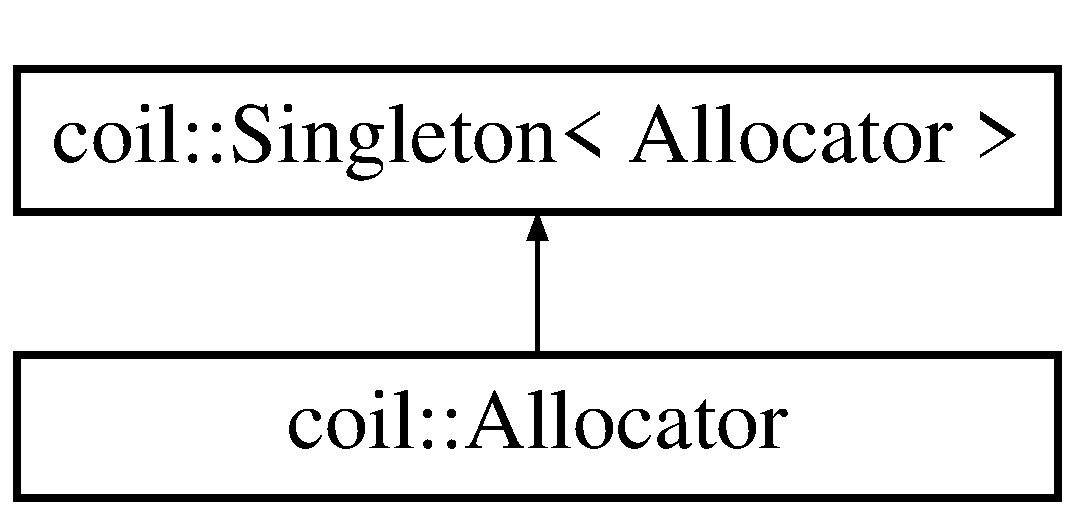
\includegraphics[height=2cm]{classcoil_1_1Allocator}
\end{center}
\end{figure}
\subsection*{Public メソッド}
\begin{DoxyCompactItemize}
\item 
virtual {\bf $\sim$Allocator} ()
\begin{DoxyCompactList}\small\item\em デストラクタ \item\end{DoxyCompactList}\item 
virtual void $\ast$ {\bf New} (size\_\-t t)  throw (std::bad\_\-alloc)
\begin{DoxyCompactList}\small\item\em メモリ領域確保 \item\end{DoxyCompactList}\item 
virtual void {\bf Delete} (void $\ast$p)  throw ()
\begin{DoxyCompactList}\small\item\em メモリ領域解放 \item\end{DoxyCompactList}\item 
virtual void $\ast$ {\bf NewArray} (size\_\-t t)  throw (std::bad\_\-alloc)
\begin{DoxyCompactList}\small\item\em 配列用メモリ領域確保 \item\end{DoxyCompactList}\item 
virtual void {\bf DeleteArray} (void $\ast$p)  throw ()
\begin{DoxyCompactList}\small\item\em 配列用メモリ領域解放 \item\end{DoxyCompactList}\end{DoxyCompactItemize}


\subsection{説明}
\doxyref{Allocator}{p.}{classcoil_1_1Allocator} クラス. 

\subsection{コンストラクタとデストラクタ}
\index{coil::Allocator@{coil::Allocator}!$\sim$Allocator@{$\sim$Allocator}}
\index{$\sim$Allocator@{$\sim$Allocator}!coil::Allocator@{coil::Allocator}}
\subsubsection[{$\sim$Allocator}]{\setlength{\rightskip}{0pt plus 5cm}virtual coil::Allocator::$\sim$Allocator ()\hspace{0.3cm}{\ttfamily  [inline, virtual]}}\label{classcoil_1_1Allocator_a4ddf0d97ba85758bc3b23227a8dd9cb6}


デストラクタ 

デストラクタ。 

\subsection{関数}
\index{coil::Allocator@{coil::Allocator}!Delete@{Delete}}
\index{Delete@{Delete}!coil::Allocator@{coil::Allocator}}
\subsubsection[{Delete}]{\setlength{\rightskip}{0pt plus 5cm}virtual void coil::Allocator::Delete (void $\ast$ {\em p})  throw ()\hspace{0.3cm}{\ttfamily  [virtual]}}\label{classcoil_1_1Allocator_a75e74a4664cbafc49bdc9e2ed4d2d8a8}


メモリ領域解放 

メモリ領域を解放する。


\begin{DoxyParams}{引数}
\item[{\em p}]メモリ領域へのポインタ \end{DoxyParams}
\index{coil::Allocator@{coil::Allocator}!DeleteArray@{DeleteArray}}
\index{DeleteArray@{DeleteArray}!coil::Allocator@{coil::Allocator}}
\subsubsection[{DeleteArray}]{\setlength{\rightskip}{0pt plus 5cm}virtual void coil::Allocator::DeleteArray (void $\ast$ {\em p})  throw ()\hspace{0.3cm}{\ttfamily  [virtual]}}\label{classcoil_1_1Allocator_ad3239ab9cf554cfe16e93be8109d83bc}


配列用メモリ領域解放 

配列用メモリ領域を解放する。


\begin{DoxyParams}{引数}
\item[{\em p}]メモリ領域へのポインタ \end{DoxyParams}
\index{coil::Allocator@{coil::Allocator}!New@{New}}
\index{New@{New}!coil::Allocator@{coil::Allocator}}
\subsubsection[{New}]{\setlength{\rightskip}{0pt plus 5cm}virtual void$\ast$ coil::Allocator::New (size\_\-t {\em t})  throw (std::bad\_\-alloc)\hspace{0.3cm}{\ttfamily  [virtual]}}\label{classcoil_1_1Allocator_a5f57ccb211ac241c2eb9845865eedfaf}


メモリ領域確保 

メモリ領域を確保する。


\begin{DoxyParams}{引数}
\item[{\em t}]割り当てサイズ\end{DoxyParams}
\begin{DoxyReturn}{戻り値}
メモリ領域へのポインタ 
\end{DoxyReturn}
\index{coil::Allocator@{coil::Allocator}!NewArray@{NewArray}}
\index{NewArray@{NewArray}!coil::Allocator@{coil::Allocator}}
\subsubsection[{NewArray}]{\setlength{\rightskip}{0pt plus 5cm}virtual void$\ast$ coil::Allocator::NewArray (size\_\-t {\em t})  throw (std::bad\_\-alloc)\hspace{0.3cm}{\ttfamily  [virtual]}}\label{classcoil_1_1Allocator_aa614febe55894d46ce0c319418d4cc04}


配列用メモリ領域確保 

配列用メモリ領域を確保する。


\begin{DoxyParams}{引数}
\item[{\em t}]割り当てサイズ\end{DoxyParams}
\begin{DoxyReturn}{戻り値}
メモリ領域へのポインタ 
\end{DoxyReturn}

\section{coil::Async Class Reference}
\label{classcoil_1_1Async}\index{coil::Async@{coil::Async}}


\doxyref{Async}{p.}{classcoil_1_1Async} class.  




{\ttfamily \#include $<$Async.h$>$}

Inheritance diagram for coil::Async:\begin{figure}[H]
\begin{center}
\leavevmode
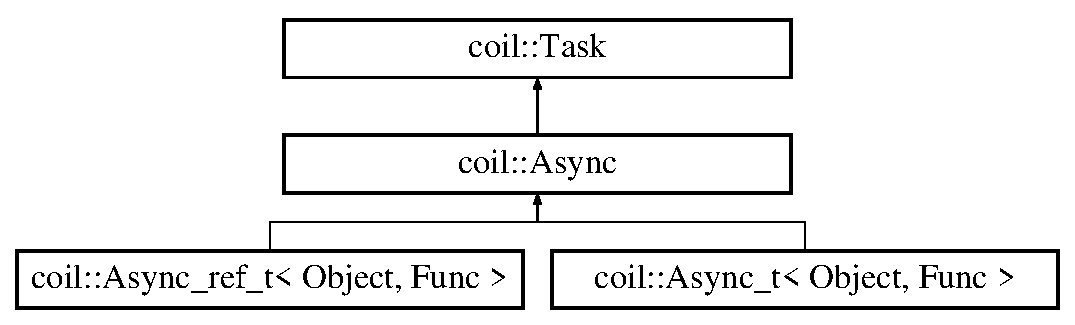
\includegraphics[height=3cm]{classcoil_1_1Async}
\end{center}
\end{figure}
\subsection*{Public Member Functions}
\begin{DoxyCompactItemize}
\item 
{\bf Async} ()
\begin{DoxyCompactList}\small\item\em Constructor. \item\end{DoxyCompactList}\item 
virtual {\bf $\sim$Async} ()
\begin{DoxyCompactList}\small\item\em Destructor. \item\end{DoxyCompactList}\item 
virtual void {\bf invoke} ()=0
\begin{DoxyCompactList}\small\item\em Asynchronous invocation. \item\end{DoxyCompactList}\item 
virtual bool {\bf finished} ()=0
\begin{DoxyCompactList}\small\item\em Check on completion state. \item\end{DoxyCompactList}\end{DoxyCompactItemize}


\subsection{Detailed Description}
\doxyref{Async}{p.}{classcoil_1_1Async} class. 

\subsection{Constructor \& Destructor Documentation}
\index{coil::Async@{coil::Async}!Async@{Async}}
\index{Async@{Async}!coil::Async@{coil::Async}}
\subsubsection[{Async}]{\setlength{\rightskip}{0pt plus 5cm}coil::Async::Async ()\hspace{0.3cm}{\ttfamily  [inline]}}\label{classcoil_1_1Async_a91ae54f017184f8a59920f5264561072}


Constructor. 

Constructor \index{coil::Async@{coil::Async}!$\sim$Async@{$\sim$Async}}
\index{$\sim$Async@{$\sim$Async}!coil::Async@{coil::Async}}
\subsubsection[{$\sim$Async}]{\setlength{\rightskip}{0pt plus 5cm}virtual coil::Async::$\sim$Async ()\hspace{0.3cm}{\ttfamily  [inline, virtual]}}\label{classcoil_1_1Async_ac38f68a3d5cb896cc0ae40a1bdc5a5e6}


Destructor. 

Destructor 

\subsection{Member Function Documentation}
\index{coil::Async@{coil::Async}!finished@{finished}}
\index{finished@{finished}!coil::Async@{coil::Async}}
\subsubsection[{finished}]{\setlength{\rightskip}{0pt plus 5cm}virtual bool coil::Async::finished ()\hspace{0.3cm}{\ttfamily  [pure virtual]}}\label{classcoil_1_1Async_a791b91a66a98acec44e63b0c5fae8b20}


Check on completion state. 

Pure virtual function for check on completion state.

\begin{DoxyReturn}{Returns}
true: finished, false: unfinished 
\end{DoxyReturn}


Implemented in {\bf coil::Async\_\-t$<$ Object, Func $>$} \doxyref{}{p.}{classcoil_1_1Async__t_af7c59952bc29131e36ee456d23bdf746}, and {\bf coil::Async\_\-ref\_\-t$<$ Object, Func $>$} \doxyref{}{p.}{classcoil_1_1Async__ref__t_a9f47a1903293a0f6f53041f42b30368b}.

\index{coil::Async@{coil::Async}!invoke@{invoke}}
\index{invoke@{invoke}!coil::Async@{coil::Async}}
\subsubsection[{invoke}]{\setlength{\rightskip}{0pt plus 5cm}virtual void coil::Async::invoke ()\hspace{0.3cm}{\ttfamily  [pure virtual]}}\label{classcoil_1_1Async_ada31d64682effe5daa79212d07c02b65}


Asynchronous invocation. 

Pure virtual function for Asynchronous invocation. 

Implemented in {\bf coil::Async\_\-t$<$ Object, Func $>$} \doxyref{}{p.}{classcoil_1_1Async__t_aa6b4d79bed3225128f3e5cbde7d0fef8}, and {\bf coil::Async\_\-ref\_\-t$<$ Object, Func $>$} \doxyref{}{p.}{classcoil_1_1Async__ref__t_a6be7d1b1d810323d89e8bf9c00f5874a}.


\section{coil::Async\_\-ref\_\-t$<$ Object, Func $>$ Class Template Reference}
\label{classcoil_1_1Async__ref__t}\index{coil::Async\_\-ref\_\-t@{coil::Async\_\-ref\_\-t}}


\doxyref{Async\_\-ref\_\-t}{p.}{classcoil_1_1Async__ref__t} template class.  




{\ttfamily \#include $<$Async.h$>$}

Inheritance diagram for coil::Async\_\-ref\_\-t$<$ Object, Func $>$:\begin{figure}[H]
\begin{center}
\leavevmode
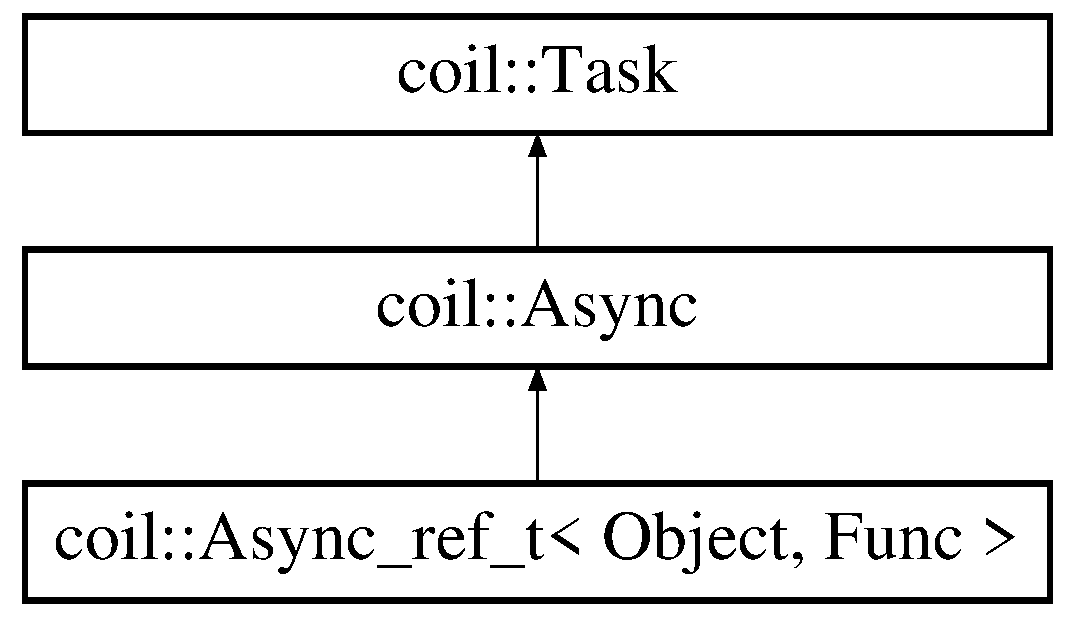
\includegraphics[height=3cm]{classcoil_1_1Async__ref__t}
\end{center}
\end{figure}
\subsection*{Public Member Functions}
\begin{DoxyCompactItemize}
\item 
{\bf Async\_\-ref\_\-t} (Object $\ast$obj, Func \&func, bool auto\_\-delete=false)
\begin{DoxyCompactList}\small\item\em Constructor. \item\end{DoxyCompactList}\item 
virtual {\bf $\sim$Async\_\-ref\_\-t} ()
\begin{DoxyCompactList}\small\item\em Destructor. \item\end{DoxyCompactList}\item 
virtual int {\bf svc} ()
\begin{DoxyCompactList}\small\item\em Thread execution function for asynchronous invoke. \item\end{DoxyCompactList}\item 
virtual void {\bf invoke} ()
\begin{DoxyCompactList}\small\item\em Asynchronous function Activation. \item\end{DoxyCompactList}\item 
virtual bool {\bf finished} ()
\begin{DoxyCompactList}\small\item\em Check on completion state. \item\end{DoxyCompactList}\item 
virtual void {\bf finalize} ()
\begin{DoxyCompactList}\small\item\em Finalize the asynchronous function. \item\end{DoxyCompactList}\end{DoxyCompactItemize}


\subsection{Detailed Description}
\subsubsection*{template$<$typename Object, typename Func$>$ class coil::Async\_\-ref\_\-t$<$ Object, Func $>$}

\doxyref{Async\_\-ref\_\-t}{p.}{classcoil_1_1Async__ref__t} template class. 

\subsection{Constructor \& Destructor Documentation}
\index{coil::Async\_\-ref\_\-t@{coil::Async\_\-ref\_\-t}!Async\_\-ref\_\-t@{Async\_\-ref\_\-t}}
\index{Async\_\-ref\_\-t@{Async\_\-ref\_\-t}!coil::Async_ref_t@{coil::Async\_\-ref\_\-t}}
\subsubsection[{Async\_\-ref\_\-t}]{\setlength{\rightskip}{0pt plus 5cm}template$<$typename Object, typename Func$>$ {\bf coil::Async\_\-ref\_\-t}$<$ Object, Func $>$::{\bf Async\_\-ref\_\-t} (Object $\ast$ {\em obj}, \/  Func \& {\em func}, \/  bool {\em auto\_\-delete} = {\ttfamily false})\hspace{0.3cm}{\ttfamily  [inline]}}\label{classcoil_1_1Async__ref__t_a9c9e02a04d699dbd488653a633f20383}


Constructor. 

Constructor


\begin{DoxyParams}{Parameters}
\item[{\em obj}]The target object for the asynchronous function. \item[{\em func}]Asynchronous function. \item[{\em auto\_\-delete}]flag for automatic instance destruction. \end{DoxyParams}
\index{coil::Async\_\-ref\_\-t@{coil::Async\_\-ref\_\-t}!$\sim$Async\_\-ref\_\-t@{$\sim$Async\_\-ref\_\-t}}
\index{$\sim$Async\_\-ref\_\-t@{$\sim$Async\_\-ref\_\-t}!coil::Async_ref_t@{coil::Async\_\-ref\_\-t}}
\subsubsection[{$\sim$Async\_\-ref\_\-t}]{\setlength{\rightskip}{0pt plus 5cm}template$<$typename Object, typename Func$>$ virtual {\bf coil::Async\_\-ref\_\-t}$<$ Object, Func $>$::$\sim${\bf Async\_\-ref\_\-t} ()\hspace{0.3cm}{\ttfamily  [inline, virtual]}}\label{classcoil_1_1Async__ref__t_aae2afa89f0a4f9c59db0a630d792751c}


Destructor. 

Destructor 

\subsection{Member Function Documentation}
\index{coil::Async\_\-ref\_\-t@{coil::Async\_\-ref\_\-t}!finalize@{finalize}}
\index{finalize@{finalize}!coil::Async_ref_t@{coil::Async\_\-ref\_\-t}}
\subsubsection[{finalize}]{\setlength{\rightskip}{0pt plus 5cm}template$<$typename Object, typename Func$>$ virtual void {\bf coil::Async\_\-ref\_\-t}$<$ Object, Func $>$::finalize ()\hspace{0.3cm}{\ttfamily  [inline, virtual]}}\label{classcoil_1_1Async__ref__t_a3aa9d20e422e78db584ead57a50200da}


Finalize the asynchronous function. 

Finalize the asynchronous function for preparing it for destruction. 

Reimplemented from {\bf coil::Task} \doxyref{}{p.}{classcoil_1_1Task_af7cfcc8cf5c0c322739a92374ce05cca}.

\index{coil::Async\_\-ref\_\-t@{coil::Async\_\-ref\_\-t}!finished@{finished}}
\index{finished@{finished}!coil::Async_ref_t@{coil::Async\_\-ref\_\-t}}
\subsubsection[{finished}]{\setlength{\rightskip}{0pt plus 5cm}template$<$typename Object, typename Func$>$ virtual bool {\bf coil::Async\_\-ref\_\-t}$<$ Object, Func $>$::finished ()\hspace{0.3cm}{\ttfamily  [inline, virtual]}}\label{classcoil_1_1Async__ref__t_a9f47a1903293a0f6f53041f42b30368b}


Check on completion state. 

Return a completion state.

\begin{DoxyReturn}{Returns}
true: finished, false: unfinished 
\end{DoxyReturn}


Implements {\bf coil::Async} \doxyref{}{p.}{classcoil_1_1Async_a791b91a66a98acec44e63b0c5fae8b20}.

\index{coil::Async\_\-ref\_\-t@{coil::Async\_\-ref\_\-t}!invoke@{invoke}}
\index{invoke@{invoke}!coil::Async_ref_t@{coil::Async\_\-ref\_\-t}}
\subsubsection[{invoke}]{\setlength{\rightskip}{0pt plus 5cm}template$<$typename Object, typename Func$>$ virtual void {\bf coil::Async\_\-ref\_\-t}$<$ Object, Func $>$::invoke ()\hspace{0.3cm}{\ttfamily  [inline, virtual]}}\label{classcoil_1_1Async__ref__t_a6be7d1b1d810323d89e8bf9c00f5874a}


Asynchronous function Activation. 

Activate of Asynchronous function. 

Implements {\bf coil::Async} \doxyref{}{p.}{classcoil_1_1Async_ada31d64682effe5daa79212d07c02b65}.



References coil::Task::activate().

\index{coil::Async\_\-ref\_\-t@{coil::Async\_\-ref\_\-t}!svc@{svc}}
\index{svc@{svc}!coil::Async_ref_t@{coil::Async\_\-ref\_\-t}}
\subsubsection[{svc}]{\setlength{\rightskip}{0pt plus 5cm}template$<$typename Object, typename Func$>$ virtual int {\bf coil::Async\_\-ref\_\-t}$<$ Object, Func $>$::svc (void)\hspace{0.3cm}{\ttfamily  [inline, virtual]}}\label{classcoil_1_1Async__ref__t_a0faaac2e307957306e4a5f093aa39d26}


Thread execution function for asynchronous invoke. 

Invoke the registered objects operation.

\begin{DoxyReturn}{Returns}
The execution result. 
\end{DoxyReturn}


Reimplemented from {\bf coil::Task} \doxyref{}{p.}{classcoil_1_1Task_ae68f22a4afbe8cddde1fe910bc3dd226}.


\section{coil::Async\_\-t$<$ Object, Func $>$ Class Template Reference}
\label{classcoil_1_1Async__t}\index{coil::Async\_\-t@{coil::Async\_\-t}}


\doxyref{Async\_\-t}{p.}{classcoil_1_1Async__t} template class.  




{\ttfamily \#include $<$Async.h$>$}

Inheritance diagram for coil::Async\_\-t$<$ Object, Func $>$:\begin{figure}[H]
\begin{center}
\leavevmode
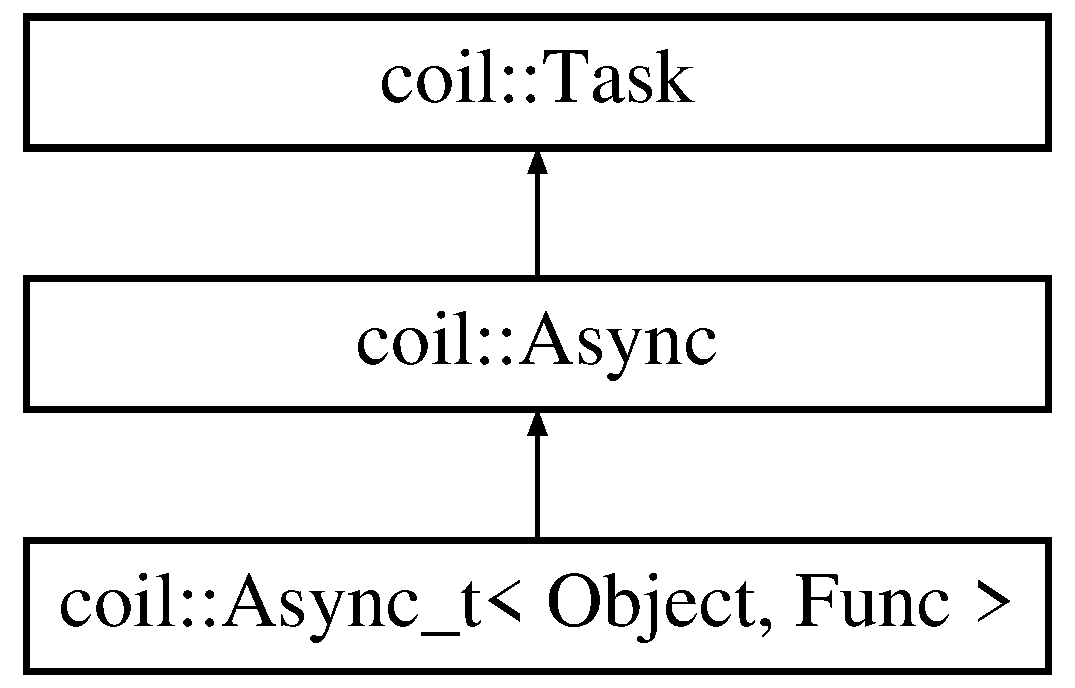
\includegraphics[height=3cm]{classcoil_1_1Async__t}
\end{center}
\end{figure}
\subsection*{Public Member Functions}
\begin{DoxyCompactItemize}
\item 
{\bf Async\_\-t} (Object $\ast$obj, Func func, bool auto\_\-delete=false)
\begin{DoxyCompactList}\small\item\em Constructor. \item\end{DoxyCompactList}\item 
virtual {\bf $\sim$Async\_\-t} ()
\begin{DoxyCompactList}\small\item\em Destructor. \item\end{DoxyCompactList}\item 
virtual int {\bf svc} ()
\begin{DoxyCompactList}\small\item\em Thread execution function for asynchronous invoke. \item\end{DoxyCompactList}\item 
virtual void {\bf finalize} ()
\begin{DoxyCompactList}\small\item\em Finalize the asynchronous function. \item\end{DoxyCompactList}\item 
virtual void {\bf invoke} ()
\begin{DoxyCompactList}\small\item\em Asynchronous function Activation. \item\end{DoxyCompactList}\item 
virtual bool {\bf finished} ()
\begin{DoxyCompactList}\small\item\em Check on completion state. \item\end{DoxyCompactList}\end{DoxyCompactItemize}


\subsection{Detailed Description}
\subsubsection*{template$<$typename Object, typename Func$>$ class coil::Async\_\-t$<$ Object, Func $>$}

\doxyref{Async\_\-t}{p.}{classcoil_1_1Async__t} template class. 

\subsection{Constructor \& Destructor Documentation}
\index{coil::Async\_\-t@{coil::Async\_\-t}!Async\_\-t@{Async\_\-t}}
\index{Async\_\-t@{Async\_\-t}!coil::Async_t@{coil::Async\_\-t}}
\subsubsection[{Async\_\-t}]{\setlength{\rightskip}{0pt plus 5cm}template$<$typename Object, typename Func$>$ {\bf coil::Async\_\-t}$<$ Object, Func $>$::{\bf Async\_\-t} (Object $\ast$ {\em obj}, \/  Func {\em func}, \/  bool {\em auto\_\-delete} = {\ttfamily false})\hspace{0.3cm}{\ttfamily  [inline]}}\label{classcoil_1_1Async__t_a164cb08198f5f690675e843d89677991}


Constructor. 

Constructor


\begin{DoxyParams}{Parameters}
\item[{\em obj}]The target object for the asynchronous function. \item[{\em func}]Asynchronous function. \item[{\em auto\_\-delete}]flag for automatic instance destruction. \end{DoxyParams}
\index{coil::Async\_\-t@{coil::Async\_\-t}!$\sim$Async\_\-t@{$\sim$Async\_\-t}}
\index{$\sim$Async\_\-t@{$\sim$Async\_\-t}!coil::Async_t@{coil::Async\_\-t}}
\subsubsection[{$\sim$Async\_\-t}]{\setlength{\rightskip}{0pt plus 5cm}template$<$typename Object, typename Func$>$ virtual {\bf coil::Async\_\-t}$<$ Object, Func $>$::$\sim${\bf Async\_\-t} ()\hspace{0.3cm}{\ttfamily  [inline, virtual]}}\label{classcoil_1_1Async__t_afbda05450d027b0d0357283a264763c9}


Destructor. 

Destructor 

\subsection{Member Function Documentation}
\index{coil::Async\_\-t@{coil::Async\_\-t}!finalize@{finalize}}
\index{finalize@{finalize}!coil::Async_t@{coil::Async\_\-t}}
\subsubsection[{finalize}]{\setlength{\rightskip}{0pt plus 5cm}template$<$typename Object, typename Func$>$ virtual void {\bf coil::Async\_\-t}$<$ Object, Func $>$::finalize ()\hspace{0.3cm}{\ttfamily  [inline, virtual]}}\label{classcoil_1_1Async__t_aaffa0e7e46f8380b0e91e5177485e00d}


Finalize the asynchronous function. 

Finalize the asynchronous function for preparing it for destruction. 

Reimplemented from {\bf coil::Task} \doxyref{}{p.}{classcoil_1_1Task_af7cfcc8cf5c0c322739a92374ce05cca}.

\index{coil::Async\_\-t@{coil::Async\_\-t}!finished@{finished}}
\index{finished@{finished}!coil::Async_t@{coil::Async\_\-t}}
\subsubsection[{finished}]{\setlength{\rightskip}{0pt plus 5cm}template$<$typename Object, typename Func$>$ virtual bool {\bf coil::Async\_\-t}$<$ Object, Func $>$::finished ()\hspace{0.3cm}{\ttfamily  [inline, virtual]}}\label{classcoil_1_1Async__t_af7c59952bc29131e36ee456d23bdf746}


Check on completion state. 

Return a completion state.

\begin{DoxyReturn}{Returns}
true: finished, false: unfinished 
\end{DoxyReturn}


Implements {\bf coil::Async} \doxyref{}{p.}{classcoil_1_1Async_a791b91a66a98acec44e63b0c5fae8b20}.

\index{coil::Async\_\-t@{coil::Async\_\-t}!invoke@{invoke}}
\index{invoke@{invoke}!coil::Async_t@{coil::Async\_\-t}}
\subsubsection[{invoke}]{\setlength{\rightskip}{0pt plus 5cm}template$<$typename Object, typename Func$>$ virtual void {\bf coil::Async\_\-t}$<$ Object, Func $>$::invoke ()\hspace{0.3cm}{\ttfamily  [inline, virtual]}}\label{classcoil_1_1Async__t_aa6b4d79bed3225128f3e5cbde7d0fef8}


Asynchronous function Activation. 

Activate of Asynchronous function. 

Implements {\bf coil::Async} \doxyref{}{p.}{classcoil_1_1Async_ada31d64682effe5daa79212d07c02b65}.



References coil::Task::activate().

\index{coil::Async\_\-t@{coil::Async\_\-t}!svc@{svc}}
\index{svc@{svc}!coil::Async_t@{coil::Async\_\-t}}
\subsubsection[{svc}]{\setlength{\rightskip}{0pt plus 5cm}template$<$typename Object, typename Func$>$ virtual int {\bf coil::Async\_\-t}$<$ Object, Func $>$::svc (void)\hspace{0.3cm}{\ttfamily  [inline, virtual]}}\label{classcoil_1_1Async__t_a2a935cf066cd5b3a90feb0aa19b9a4b1}


Thread execution function for asynchronous invoke. 

Invoke the registered objects operation.

\begin{DoxyReturn}{Returns}
The execution result. 
\end{DoxyReturn}


Reimplemented from {\bf coil::Task} \doxyref{}{p.}{classcoil_1_1Task_ae68f22a4afbe8cddde1fe910bc3dd226}.


\section{RTC::BufferBase$<$ DataType $>$ Class Template Reference}
\label{classRTC_1_1BufferBase}\index{RTC::BufferBase@{RTC::BufferBase}}


\doxyref{BufferBase}{p.}{classRTC_1_1BufferBase} abstract class.  




{\ttfamily \#include $<$BufferBase.h$>$}

Inheritance diagram for RTC::BufferBase$<$ DataType $>$:\begin{figure}[H]
\begin{center}
\leavevmode
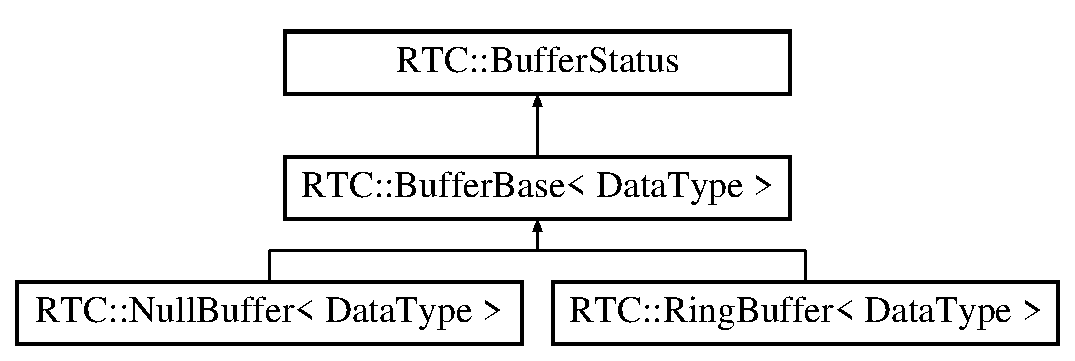
\includegraphics[height=3cm]{classRTC_1_1BufferBase}
\end{center}
\end{figure}
\subsection*{Public Member Functions}
\begin{DoxyCompactItemize}
\item 
virtual BUFFERSTATUS\_\-ENUM {\bf $\sim$BufferBase} (void)
\begin{DoxyCompactList}\small\item\em Virtual destructor. \item\end{DoxyCompactList}\item 
virtual void {\bf init} (const {\bf coil::Properties} \&prop)=0
\begin{DoxyCompactList}\small\item\em Set the buffer. \item\end{DoxyCompactList}\item 
virtual size\_\-t {\bf length} (void) const =0
\begin{DoxyCompactList}\small\item\em Get the buffer length. \item\end{DoxyCompactList}\item 
virtual ReturnCode {\bf length} (size\_\-t n)=0
\begin{DoxyCompactList}\small\item\em Set the buffer length. \item\end{DoxyCompactList}\item 
virtual ReturnCode {\bf reset} ()=0
\begin{DoxyCompactList}\small\item\em Reset the buffer status. \item\end{DoxyCompactList}\item 
virtual DataType $\ast$ {\bf wptr} (long int n=0)=0
\begin{DoxyCompactList}\small\item\em Get the writing pointer. \item\end{DoxyCompactList}\item 
virtual ReturnCode {\bf advanceWptr} (long int n=1)=0
\begin{DoxyCompactList}\small\item\em Forward n writing pointers. \item\end{DoxyCompactList}\item 
virtual ReturnCode {\bf put} (const DataType \&value)=0
\begin{DoxyCompactList}\small\item\em Write data into the buffer. \item\end{DoxyCompactList}\item 
virtual ReturnCode {\bf write} (const DataType \&value, long int sec=-\/1, long int nsec=-\/1)=0
\begin{DoxyCompactList}\small\item\em Write data into the buffer. \item\end{DoxyCompactList}\item 
virtual size\_\-t {\bf writable} () const =0
\begin{DoxyCompactList}\small\item\em Get a writable number. \item\end{DoxyCompactList}\item 
virtual bool {\bf full} (void) const =0
\begin{DoxyCompactList}\small\item\em Check on whether the buffer is full. \item\end{DoxyCompactList}\item 
virtual DataType $\ast$ {\bf rptr} (long int n=0)=0
\begin{DoxyCompactList}\small\item\em Get the reading pointer. \item\end{DoxyCompactList}\item 
virtual ReturnCode {\bf advanceRptr} (long int n=1)=0
\begin{DoxyCompactList}\small\item\em Forward n reading pointers. \item\end{DoxyCompactList}\item 
virtual ReturnCode {\bf get} (DataType \&value)=0
\begin{DoxyCompactList}\small\item\em Read data from the buffer. \item\end{DoxyCompactList}\item 
virtual DataType \& {\bf get} ()=0
\begin{DoxyCompactList}\small\item\em Read data from the buffer. \item\end{DoxyCompactList}\item 
virtual ReturnCode {\bf read} (DataType \&value, long int sec=-\/1, long int nsec=-\/1)=0
\begin{DoxyCompactList}\small\item\em Read data from the buffer. \item\end{DoxyCompactList}\item 
virtual size\_\-t {\bf readable} () const =0
\begin{DoxyCompactList}\small\item\em Write data into the buffer. \item\end{DoxyCompactList}\item 
virtual bool {\bf empty} (void) const =0
\begin{DoxyCompactList}\small\item\em Check on whether the buffer is empty. \item\end{DoxyCompactList}\end{DoxyCompactItemize}


\subsection{Detailed Description}
\subsubsection*{template$<$class DataType$>$ class RTC::BufferBase$<$ DataType $>$}

\doxyref{BufferBase}{p.}{classRTC_1_1BufferBase} abstract class. This is the abstract interface class for various Buffer. Concrete buffer classes must implement the following pure virtual functions. The users specify data type to hold it in a buffer as $<$DataType$>$.

This class provides public interface as follows.
\begin{DoxyItemize}
\item \doxyref{write()}{p.}{classRTC_1_1BufferBase_ad9df647826ca2f05664aa0f53e4142f7}: Write data into the buffer.
\item \doxyref{read()}{p.}{classRTC_1_1BufferBase_a92f188cb4e9a92c9c1079273b1deadc0}: Read data from the buffer.
\item \doxyref{length()}{p.}{classRTC_1_1BufferBase_ad41d5476f9bce0e737115e8ab7cc615f}: Get the buffer length.
\item isFull(): Check on whether the buffer is full.
\item isEmpty(): Check on whether the buffer is empty.
\end{DoxyItemize}

This class provides protected interface as follows.
\begin{DoxyItemize}
\item \doxyref{put()}{p.}{classRTC_1_1BufferBase_af6274c9bc458580643560752f9150235}: Store data into the buffer.
\item \doxyref{get()}{p.}{classRTC_1_1BufferBase_af12dcf239b3842fe6c946cb61c3d0bd2}: Get data from the buffer.
\end{DoxyItemize}


\begin{DoxyParams}{Parameters}
\item[{\em DataType}]Data type to be stored to the buffer.\end{DoxyParams}
\begin{DoxySince}{Since}
0.4.0 
\end{DoxySince}


\subsection{Constructor \& Destructor Documentation}
\index{RTC::BufferBase@{RTC::BufferBase}!$\sim$BufferBase@{$\sim$BufferBase}}
\index{$\sim$BufferBase@{$\sim$BufferBase}!RTC::BufferBase@{RTC::BufferBase}}
\subsubsection[{$\sim$BufferBase}]{\setlength{\rightskip}{0pt plus 5cm}template$<$class DataType$>$ virtual BUFFERSTATUS\_\-ENUM {\bf RTC::BufferBase}$<$ DataType $>$::$\sim${\bf BufferBase} (void)\hspace{0.3cm}{\ttfamily  [inline, virtual]}}\label{classRTC_1_1BufferBase_a9d5cf204b02ee64d7ebf8f3754e2610d}


Virtual destructor. 



\subsection{Member Function Documentation}
\index{RTC::BufferBase@{RTC::BufferBase}!advanceRptr@{advanceRptr}}
\index{advanceRptr@{advanceRptr}!RTC::BufferBase@{RTC::BufferBase}}
\subsubsection[{advanceRptr}]{\setlength{\rightskip}{0pt plus 5cm}template$<$class DataType$>$ virtual ReturnCode {\bf RTC::BufferBase}$<$ DataType $>$::advanceRptr (long int {\em n} = {\ttfamily 1})\hspace{0.3cm}{\ttfamily  [pure virtual]}}\label{classRTC_1_1BufferBase_aebc3b8b032109963dfa0e3c48f59a333}


Forward n reading pointers. 

Pure virtual function to forward n reading pointers.

\begin{DoxyReturn}{Returns}
BUFFER\_\-OK: Successful BUFFER\_\-ERROR: Failed 
\end{DoxyReturn}


Implemented in {\bf RTC::RingBuffer$<$ DataType $>$} \doxyref{}{p.}{classRTC_1_1RingBuffer_a329834c2988670fa5f849923e9070ed8}.

\index{RTC::BufferBase@{RTC::BufferBase}!advanceWptr@{advanceWptr}}
\index{advanceWptr@{advanceWptr}!RTC::BufferBase@{RTC::BufferBase}}
\subsubsection[{advanceWptr}]{\setlength{\rightskip}{0pt plus 5cm}template$<$class DataType$>$ virtual ReturnCode {\bf RTC::BufferBase}$<$ DataType $>$::advanceWptr (long int {\em n} = {\ttfamily 1})\hspace{0.3cm}{\ttfamily  [pure virtual]}}\label{classRTC_1_1BufferBase_a75c0360e0621ebfcbd08e6e937d03ed2}


Forward n writing pointers. 

Pure virtual function to forward n writing pointers.

\begin{DoxyReturn}{Returns}
BUFFER\_\-OK: Successful BUFFER\_\-ERROR: Failed 
\end{DoxyReturn}


Implemented in {\bf RTC::RingBuffer$<$ DataType $>$} \doxyref{}{p.}{classRTC_1_1RingBuffer_a208c5454c6466f09a6cb1cbcd1297871}.

\index{RTC::BufferBase@{RTC::BufferBase}!empty@{empty}}
\index{empty@{empty}!RTC::BufferBase@{RTC::BufferBase}}
\subsubsection[{empty}]{\setlength{\rightskip}{0pt plus 5cm}template$<$class DataType$>$ virtual bool {\bf RTC::BufferBase}$<$ DataType $>$::empty (void) const\hspace{0.3cm}{\ttfamily  [pure virtual]}}\label{classRTC_1_1BufferBase_a00e5f836b601681073173740fdaa44d8}


Check on whether the buffer is empty. 

Pure virtual function to check on whether the buffer is empty.

\begin{DoxyReturn}{Returns}
True if the buffer is empty, else false. 
\end{DoxyReturn}


Implemented in {\bf RTC::RingBuffer$<$ DataType $>$} \doxyref{}{p.}{classRTC_1_1RingBuffer_ace2d405ddf45929f635ed596cd62f110}.

\index{RTC::BufferBase@{RTC::BufferBase}!full@{full}}
\index{full@{full}!RTC::BufferBase@{RTC::BufferBase}}
\subsubsection[{full}]{\setlength{\rightskip}{0pt plus 5cm}template$<$class DataType$>$ virtual bool {\bf RTC::BufferBase}$<$ DataType $>$::full (void) const\hspace{0.3cm}{\ttfamily  [pure virtual]}}\label{classRTC_1_1BufferBase_a66948bc482a6e127b0ed839a95d692b3}


Check on whether the buffer is full. 

Pure virtual function to check on whether the buffer is full.

\begin{DoxyReturn}{Returns}
True if the buffer is full, else false. 
\end{DoxyReturn}


Implemented in {\bf RTC::RingBuffer$<$ DataType $>$} \doxyref{}{p.}{classRTC_1_1RingBuffer_ae7a8906ed3de0c95ffed9dd4f5f74f3b}.

\index{RTC::BufferBase@{RTC::BufferBase}!get@{get}}
\index{get@{get}!RTC::BufferBase@{RTC::BufferBase}}
\subsubsection[{get}]{\setlength{\rightskip}{0pt plus 5cm}template$<$class DataType$>$ virtual DataType\& {\bf RTC::BufferBase}$<$ DataType $>$::get ()\hspace{0.3cm}{\ttfamily  [pure virtual]}}\label{classRTC_1_1BufferBase_af12dcf239b3842fe6c946cb61c3d0bd2}


Read data from the buffer. 

Pure virtual function to read data from the buffer.

\begin{DoxyReturn}{Returns}
Data got from buffer. 
\end{DoxyReturn}


Implemented in {\bf RTC::NullBuffer$<$ DataType $>$} \doxyref{}{p.}{classRTC_1_1NullBuffer_a5acb245659e61424bda0080b44d7b6d1}, and {\bf RTC::RingBuffer$<$ DataType $>$} \doxyref{}{p.}{classRTC_1_1RingBuffer_a229d439990825b2a829daf2f747b8b1b}.

\index{RTC::BufferBase@{RTC::BufferBase}!get@{get}}
\index{get@{get}!RTC::BufferBase@{RTC::BufferBase}}
\subsubsection[{get}]{\setlength{\rightskip}{0pt plus 5cm}template$<$class DataType$>$ virtual ReturnCode {\bf RTC::BufferBase}$<$ DataType $>$::get (DataType \& {\em value})\hspace{0.3cm}{\ttfamily  [pure virtual]}}\label{classRTC_1_1BufferBase_a82263a34b3274b316b6563ee5339a7a0}


Read data from the buffer. 

Pure virtual function to read data form the buffer.


\begin{DoxyParams}{Parameters}
\item[{\em value}]Data to read.\end{DoxyParams}
\begin{DoxyReturn}{Returns}
BUFFER\_\-OK: Successful BUFFER\_\-ERROR: Failed 
\end{DoxyReturn}


Implemented in {\bf RTC::RingBuffer$<$ DataType $>$} \doxyref{}{p.}{classRTC_1_1RingBuffer_a10506341647d0f93cbea400fe9628bf0}.

\index{RTC::BufferBase@{RTC::BufferBase}!init@{init}}
\index{init@{init}!RTC::BufferBase@{RTC::BufferBase}}
\subsubsection[{init}]{\setlength{\rightskip}{0pt plus 5cm}template$<$class DataType$>$ virtual void {\bf RTC::BufferBase}$<$ DataType $>$::init (const {\bf coil::Properties} \& {\em prop})\hspace{0.3cm}{\ttfamily  [pure virtual]}}\label{classRTC_1_1BufferBase_a75adf7ba27bb2e795761bce1c7d76413}


Set the buffer. 



Implemented in {\bf RTC::RingBuffer$<$ DataType $>$} \doxyref{}{p.}{classRTC_1_1RingBuffer_a8bd57fca9d29703083c8ff0817dc0a55}.

\index{RTC::BufferBase@{RTC::BufferBase}!length@{length}}
\index{length@{length}!RTC::BufferBase@{RTC::BufferBase}}
\subsubsection[{length}]{\setlength{\rightskip}{0pt plus 5cm}template$<$class DataType$>$ virtual ReturnCode {\bf RTC::BufferBase}$<$ DataType $>$::length (size\_\-t {\em n})\hspace{0.3cm}{\ttfamily  [pure virtual]}}\label{classRTC_1_1BufferBase_a9da737609dfc79b3f10f63ca7efc2203}


Set the buffer length. 

Pure virtual function to set the buffer length.

\begin{DoxyReturn}{Returns}
BUFFER\_\-OK: Successful NOT\_\-SUPPORTED: The buffer length cannot be set. BUFFER\_\-ERROR: Failed 
\end{DoxyReturn}


Implemented in {\bf RTC::RingBuffer$<$ DataType $>$} \doxyref{}{p.}{classRTC_1_1RingBuffer_a9584ba6385836d6936d4fda2e595136e}.

\index{RTC::BufferBase@{RTC::BufferBase}!length@{length}}
\index{length@{length}!RTC::BufferBase@{RTC::BufferBase}}
\subsubsection[{length}]{\setlength{\rightskip}{0pt plus 5cm}template$<$class DataType$>$ virtual size\_\-t {\bf RTC::BufferBase}$<$ DataType $>$::length (void) const\hspace{0.3cm}{\ttfamily  [pure virtual]}}\label{classRTC_1_1BufferBase_ad41d5476f9bce0e737115e8ab7cc615f}


Get the buffer length. 

Pure virtual function to get the buffer length.

\begin{DoxyReturn}{Returns}
buffer length 
\end{DoxyReturn}


Implemented in {\bf RTC::NullBuffer$<$ DataType $>$} \doxyref{}{p.}{classRTC_1_1NullBuffer_a10b3ecbf48ec0987e321465f21887030}, and {\bf RTC::RingBuffer$<$ DataType $>$} \doxyref{}{p.}{classRTC_1_1RingBuffer_a00c6d912326c1bc65aaf8bc2f0e8895f}.

\index{RTC::BufferBase@{RTC::BufferBase}!put@{put}}
\index{put@{put}!RTC::BufferBase@{RTC::BufferBase}}
\subsubsection[{put}]{\setlength{\rightskip}{0pt plus 5cm}template$<$class DataType$>$ virtual ReturnCode {\bf RTC::BufferBase}$<$ DataType $>$::put (const DataType \& {\em value})\hspace{0.3cm}{\ttfamily  [pure virtual]}}\label{classRTC_1_1BufferBase_af6274c9bc458580643560752f9150235}


Write data into the buffer. 

Pure virtual function to write data into the buffer.


\begin{DoxyParams}{Parameters}
\item[{\em value}]Target data to write.\end{DoxyParams}
\begin{DoxyReturn}{Returns}
BUFFER\_\-OK: Successful BUFFER\_\-ERROR: Failed 
\end{DoxyReturn}


Implemented in {\bf RTC::NullBuffer$<$ DataType $>$} \doxyref{}{p.}{classRTC_1_1NullBuffer_a0704a4190bd82c637635528ea4c28416}, and {\bf RTC::RingBuffer$<$ DataType $>$} \doxyref{}{p.}{classRTC_1_1RingBuffer_acc983b57ac5fd73a47afdfdaab1e3845}.

\index{RTC::BufferBase@{RTC::BufferBase}!read@{read}}
\index{read@{read}!RTC::BufferBase@{RTC::BufferBase}}
\subsubsection[{read}]{\setlength{\rightskip}{0pt plus 5cm}template$<$class DataType$>$ virtual ReturnCode {\bf RTC::BufferBase}$<$ DataType $>$::read (DataType \& {\em value}, \/  long int {\em sec} = {\ttfamily -\/1}, \/  long int {\em nsec} = {\ttfamily -\/1})\hspace{0.3cm}{\ttfamily  [pure virtual]}}\label{classRTC_1_1BufferBase_a92f188cb4e9a92c9c1079273b1deadc0}


Read data from the buffer. 

Pure virtual function to read data from the buffer.


\begin{DoxyParams}{Parameters}
\item[{\em value}]Read data.\end{DoxyParams}
\begin{DoxyReturn}{Returns}
Result of having read (true:Successful, false:Failed) 
\end{DoxyReturn}


Implemented in {\bf RTC::RingBuffer$<$ DataType $>$} \doxyref{}{p.}{classRTC_1_1RingBuffer_ae1b487f7b32dd15db9760b236edb0e5d}.

\index{RTC::BufferBase@{RTC::BufferBase}!readable@{readable}}
\index{readable@{readable}!RTC::BufferBase@{RTC::BufferBase}}
\subsubsection[{readable}]{\setlength{\rightskip}{0pt plus 5cm}template$<$class DataType$>$ virtual size\_\-t {\bf RTC::BufferBase}$<$ DataType $>$::readable () const\hspace{0.3cm}{\ttfamily  [pure virtual]}}\label{classRTC_1_1BufferBase_a7dd8259e299a273e2fe3744e669b381a}


Write data into the buffer. 

Pure virtual function to get a reading number.

\begin{DoxyReturn}{Returns}
readable number 
\end{DoxyReturn}


Implemented in {\bf RTC::RingBuffer$<$ DataType $>$} \doxyref{}{p.}{classRTC_1_1RingBuffer_ae5c8def9186589ac7ad53239a37fe99e}.

\index{RTC::BufferBase@{RTC::BufferBase}!reset@{reset}}
\index{reset@{reset}!RTC::BufferBase@{RTC::BufferBase}}
\subsubsection[{reset}]{\setlength{\rightskip}{0pt plus 5cm}template$<$class DataType$>$ virtual ReturnCode {\bf RTC::BufferBase}$<$ DataType $>$::reset ()\hspace{0.3cm}{\ttfamily  [pure virtual]}}\label{classRTC_1_1BufferBase_a941b36c7352c76da52725a169e094e16}


Reset the buffer status. 

Pure virtual function to reset the buffer status.

\begin{DoxyReturn}{Returns}
BUFFER\_\-OK: Successful NOT\_\-SUPPORTED: The buffer status cannot be reset. BUFFER\_\-ERROR: Failed 
\end{DoxyReturn}


Implemented in {\bf RTC::RingBuffer$<$ DataType $>$} \doxyref{}{p.}{classRTC_1_1RingBuffer_add373502f0292178296f3750d5e962a0}.

\index{RTC::BufferBase@{RTC::BufferBase}!rptr@{rptr}}
\index{rptr@{rptr}!RTC::BufferBase@{RTC::BufferBase}}
\subsubsection[{rptr}]{\setlength{\rightskip}{0pt plus 5cm}template$<$class DataType$>$ virtual DataType$\ast$ {\bf RTC::BufferBase}$<$ DataType $>$::rptr (long int {\em n} = {\ttfamily 0})\hspace{0.3cm}{\ttfamily  [pure virtual]}}\label{classRTC_1_1BufferBase_a854fd94174172b67034cf727e6c0a2d1}


Get the reading pointer. 

Pure virtual function to get the reading pointer.

\begin{DoxyReturn}{Returns}
reading pointer 
\end{DoxyReturn}


Implemented in {\bf RTC::RingBuffer$<$ DataType $>$} \doxyref{}{p.}{classRTC_1_1RingBuffer_a65401c71cb216a0730f6793f5a00dd1d}.

\index{RTC::BufferBase@{RTC::BufferBase}!wptr@{wptr}}
\index{wptr@{wptr}!RTC::BufferBase@{RTC::BufferBase}}
\subsubsection[{wptr}]{\setlength{\rightskip}{0pt plus 5cm}template$<$class DataType$>$ virtual DataType$\ast$ {\bf RTC::BufferBase}$<$ DataType $>$::wptr (long int {\em n} = {\ttfamily 0})\hspace{0.3cm}{\ttfamily  [pure virtual]}}\label{classRTC_1_1BufferBase_a27d6bb261714e84f16ef17e6920413ce}


Get the writing pointer. 

Pure virtual function to get the writing pointer.


\begin{DoxyParams}{Parameters}
\item[{\em writeing}]pinter or n previous pointer \end{DoxyParams}
\begin{DoxyReturn}{Returns}
writing pointer 
\end{DoxyReturn}


Implemented in {\bf RTC::RingBuffer$<$ DataType $>$} \doxyref{}{p.}{classRTC_1_1RingBuffer_ad9aba4e554f5fd23a1cc7b9d63b0fe07}.

\index{RTC::BufferBase@{RTC::BufferBase}!writable@{writable}}
\index{writable@{writable}!RTC::BufferBase@{RTC::BufferBase}}
\subsubsection[{writable}]{\setlength{\rightskip}{0pt plus 5cm}template$<$class DataType$>$ virtual size\_\-t {\bf RTC::BufferBase}$<$ DataType $>$::writable () const\hspace{0.3cm}{\ttfamily  [pure virtual]}}\label{classRTC_1_1BufferBase_a089b1c57c7d8aea9f1bdcc055e20bff0}


Get a writable number. 

Pure virtual function to get a writable number.

\begin{DoxyReturn}{Returns}
value writable number 
\end{DoxyReturn}


Implemented in {\bf RTC::RingBuffer$<$ DataType $>$} \doxyref{}{p.}{classRTC_1_1RingBuffer_a7bebdef8031509955d74327ccad2ceec}.

\index{RTC::BufferBase@{RTC::BufferBase}!write@{write}}
\index{write@{write}!RTC::BufferBase@{RTC::BufferBase}}
\subsubsection[{write}]{\setlength{\rightskip}{0pt plus 5cm}template$<$class DataType$>$ virtual ReturnCode {\bf RTC::BufferBase}$<$ DataType $>$::write (const DataType \& {\em value}, \/  long int {\em sec} = {\ttfamily -\/1}, \/  long int {\em nsec} = {\ttfamily -\/1})\hspace{0.3cm}{\ttfamily  [pure virtual]}}\label{classRTC_1_1BufferBase_ad9df647826ca2f05664aa0f53e4142f7}


Write data into the buffer. 

Pure virtual function to write data into the buffer.


\begin{DoxyParams}{Parameters}
\item[{\em value}]Target data to write.\end{DoxyParams}
\begin{DoxyReturn}{Returns}
BUFFER\_\-OK: Successful BUFFER\_\-ERROR: Failed 
\end{DoxyReturn}


Implemented in {\bf RTC::RingBuffer$<$ DataType $>$} \doxyref{}{p.}{classRTC_1_1RingBuffer_a4b062367982f9748b3ba5891cf753040}.


\section{RTC::BufferStatus Class Reference}
\label{classRTC_1_1BufferStatus}\index{RTC::BufferStatus@{RTC::BufferStatus}}


\doxyref{BufferStatus}{p.}{classRTC_1_1BufferStatus} mixin class.  




{\ttfamily \#include $<$BufferStatus.h$>$}

Inheritance diagram for RTC::BufferStatus:\begin{figure}[H]
\begin{center}
\leavevmode
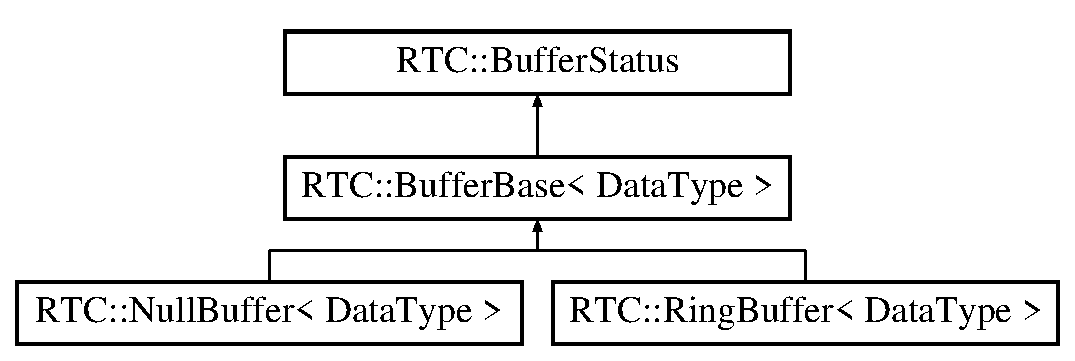
\includegraphics[height=3cm]{classRTC_1_1BufferStatus}
\end{center}
\end{figure}
\subsection*{Public Types}
\begin{DoxyCompactItemize}
\item 
enum {\bf Enum} \{ \par
{\bf BUFFER\_\-OK} =  0, 
{\bf BUFFER\_\-ERROR}, 
{\bf BUFFER\_\-FULL}, 
{\bf BUFFER\_\-EMPTY}, 
\par
{\bf NOT\_\-SUPPORTED}, 
{\bf TIMEOUT}, 
{\bf PRECONDITION\_\-NOT\_\-MET}
 \}
\begin{DoxyCompactList}\small\item\em \doxyref{DataPortStatus}{p.}{classRTC_1_1DataPortStatus} return codes. \item\end{DoxyCompactList}\end{DoxyCompactItemize}
\subsection*{Static Public Member Functions}
\begin{DoxyCompactItemize}
\item 
static const char $\ast$ {\bf toString} ({\bf Enum} status)
\begin{DoxyCompactList}\small\item\em Convert \doxyref{BufferStatus}{p.}{classRTC_1_1BufferStatus} into the string. \item\end{DoxyCompactList}\end{DoxyCompactItemize}


\subsection{Detailed Description}
\doxyref{BufferStatus}{p.}{classRTC_1_1BufferStatus} mixin class. This is a mixin class to provide enumed return codes that are commonly utilised in buffer realted sub-\/classes. To use this class, sub-\/class should inherit this class as a public super class, and declare BUFFERSTATUS\_\-ENUM defined below. Consequently, ReturnCode\_\-t type that is typedefed by this macro can be used in the sub-\/class, and enumed identifiers are imported to the class's namespace. 

\subsection{Member Enumeration Documentation}
\index{RTC::BufferStatus@{RTC::BufferStatus}!Enum@{Enum}}
\index{Enum@{Enum}!RTC::BufferStatus@{RTC::BufferStatus}}
\subsubsection[{Enum}]{\setlength{\rightskip}{0pt plus 5cm}enum {\bf RTC::BufferStatus::Enum}}\label{classRTC_1_1BufferStatus_ada857a5e7b898e1ad19caaaf7a0ff713}


\doxyref{DataPortStatus}{p.}{classRTC_1_1DataPortStatus} return codes. 

Common return codes for buffer classes.


\begin{DoxyItemize}
\item BUFFER\_\-OK: Normal return
\item BUFFER\_\-ERROR: Buffer error
\item BUFFER\_\-FULL: Buffer full
\item BUFFER\_\-EMPTY: Buffer empty
\item NOT\_\-SUPPORTED: Not supported function
\item TIMEOUT: Timeout
\item PRECONDITION\_\-NOT\_\-MET: Precodition not met 
\end{DoxyItemize}\begin{Desc}
\item[Enumerator: ]\par
\begin{description}
\index{BUFFER\_\-OK@{BUFFER\_\-OK}!RTC::BufferStatus@{RTC::BufferStatus}}\index{RTC::BufferStatus@{RTC::BufferStatus}!BUFFER\_\-OK@{BUFFER\_\-OK}}\item[{\em 
BUFFER\_\-OK\label{classRTC_1_1BufferStatus_ada857a5e7b898e1ad19caaaf7a0ff713a8f953167d31babf4fa80112461b7b388}
}]\index{BUFFER\_\-ERROR@{BUFFER\_\-ERROR}!RTC::BufferStatus@{RTC::BufferStatus}}\index{RTC::BufferStatus@{RTC::BufferStatus}!BUFFER\_\-ERROR@{BUFFER\_\-ERROR}}\item[{\em 
BUFFER\_\-ERROR\label{classRTC_1_1BufferStatus_ada857a5e7b898e1ad19caaaf7a0ff713a49a15bebcc2b15516a7cb9e930009c83}
}]\index{BUFFER\_\-FULL@{BUFFER\_\-FULL}!RTC::BufferStatus@{RTC::BufferStatus}}\index{RTC::BufferStatus@{RTC::BufferStatus}!BUFFER\_\-FULL@{BUFFER\_\-FULL}}\item[{\em 
BUFFER\_\-FULL\label{classRTC_1_1BufferStatus_ada857a5e7b898e1ad19caaaf7a0ff713acee7ab71be75d777a36e6f43450e3a96}
}]\index{BUFFER\_\-EMPTY@{BUFFER\_\-EMPTY}!RTC::BufferStatus@{RTC::BufferStatus}}\index{RTC::BufferStatus@{RTC::BufferStatus}!BUFFER\_\-EMPTY@{BUFFER\_\-EMPTY}}\item[{\em 
BUFFER\_\-EMPTY\label{classRTC_1_1BufferStatus_ada857a5e7b898e1ad19caaaf7a0ff713a4938f8154da3c9f7cad45f738b913580}
}]\index{NOT\_\-SUPPORTED@{NOT\_\-SUPPORTED}!RTC::BufferStatus@{RTC::BufferStatus}}\index{RTC::BufferStatus@{RTC::BufferStatus}!NOT\_\-SUPPORTED@{NOT\_\-SUPPORTED}}\item[{\em 
NOT\_\-SUPPORTED\label{classRTC_1_1BufferStatus_ada857a5e7b898e1ad19caaaf7a0ff713ad1f406fba36f7e517cdb68d804b861d3}
}]\index{TIMEOUT@{TIMEOUT}!RTC::BufferStatus@{RTC::BufferStatus}}\index{RTC::BufferStatus@{RTC::BufferStatus}!TIMEOUT@{TIMEOUT}}\item[{\em 
TIMEOUT\label{classRTC_1_1BufferStatus_ada857a5e7b898e1ad19caaaf7a0ff713a2024553338d0b9dc6edb25af7cdaced8}
}]\index{PRECONDITION\_\-NOT\_\-MET@{PRECONDITION\_\-NOT\_\-MET}!RTC::BufferStatus@{RTC::BufferStatus}}\index{RTC::BufferStatus@{RTC::BufferStatus}!PRECONDITION\_\-NOT\_\-MET@{PRECONDITION\_\-NOT\_\-MET}}\item[{\em 
PRECONDITION\_\-NOT\_\-MET\label{classRTC_1_1BufferStatus_ada857a5e7b898e1ad19caaaf7a0ff713aaaa1b8912b339e6f4af393294645f220}
}]\end{description}
\end{Desc}



\subsection{Member Function Documentation}
\index{RTC::BufferStatus@{RTC::BufferStatus}!toString@{toString}}
\index{toString@{toString}!RTC::BufferStatus@{RTC::BufferStatus}}
\subsubsection[{toString}]{\setlength{\rightskip}{0pt plus 5cm}static const char$\ast$ RTC::BufferStatus::toString ({\bf Enum} {\em status})\hspace{0.3cm}{\ttfamily  [inline, static]}}\label{classRTC_1_1BufferStatus_aa7b5d507e0b71878da0491ee39d7f1bc}


Convert \doxyref{BufferStatus}{p.}{classRTC_1_1BufferStatus} into the string. 

Convert \doxyref{BufferStatus}{p.}{classRTC_1_1BufferStatus} into the string.


\begin{DoxyParams}{Parameters}
\item[{\em status}]The target \doxyref{BufferStatus}{p.}{classRTC_1_1BufferStatus} for transformation\end{DoxyParams}
\begin{DoxyReturn}{Returns}
Trnasformation result of string representation 
\end{DoxyReturn}

\section{RTC::PeriodicExecutionContext::Comp Struct Reference}
\label{structRTC_1_1PeriodicExecutionContext_1_1Comp}\index{RTC::PeriodicExecutionContext::Comp@{RTC::PeriodicExecutionContext::Comp}}


The structure for the component management.  




{\ttfamily \#include $<$PeriodicExecutionContext.h$>$}

\subsection*{Public Member Functions}
\begin{DoxyCompactItemize}
\item 
{\bf Comp} (LightweightRTObject\_\-ptr ref, OpenRTM::DataFlowComponent\_\-ptr dfp, ExecutionContextHandle\_\-t id)
\item 
{\bf $\sim$Comp} (void)
\item 
{\bf Comp} (const {\bf Comp} \&comp)
\item 
{\bf Comp} \& {\bf operator=} (const {\bf Comp} \&comp)
\end{DoxyCompactItemize}
\subsection*{Public Attributes}
\begin{DoxyCompactItemize}
\item 
LightweightRTObject\_\-var {\bf \_\-ref}
\item 
{\bf DFP}$<$ OpenRTM::DataFlowComponent\_\-var $>$ {\bf \_\-sm}
\end{DoxyCompactItemize}


\subsection{Detailed Description}
The structure for the component management. 

\subsection{Constructor \& Destructor Documentation}
\index{RTC::PeriodicExecutionContext::Comp@{RTC::PeriodicExecutionContext::Comp}!Comp@{Comp}}
\index{Comp@{Comp}!RTC::PeriodicExecutionContext::Comp@{RTC::PeriodicExecutionContext::Comp}}
\subsubsection[{Comp}]{\setlength{\rightskip}{0pt plus 5cm}RTC::PeriodicExecutionContext::Comp::Comp (LightweightRTObject\_\-ptr {\em ref}, \/  OpenRTM::DataFlowComponent\_\-ptr {\em dfp}, \/  ExecutionContextHandle\_\-t {\em id})\hspace{0.3cm}{\ttfamily  [inline]}}\label{structRTC_1_1PeriodicExecutionContext_1_1Comp_a9dc4712ecec7794a3523c8982f65ce93}
\index{RTC::PeriodicExecutionContext::Comp@{RTC::PeriodicExecutionContext::Comp}!$\sim$Comp@{$\sim$Comp}}
\index{$\sim$Comp@{$\sim$Comp}!RTC::PeriodicExecutionContext::Comp@{RTC::PeriodicExecutionContext::Comp}}
\subsubsection[{$\sim$Comp}]{\setlength{\rightskip}{0pt plus 5cm}RTC::PeriodicExecutionContext::Comp::$\sim$Comp (void)\hspace{0.3cm}{\ttfamily  [inline]}}\label{structRTC_1_1PeriodicExecutionContext_1_1Comp_aa480b2328ec2db51a2db87303f9ddcd5}
\index{RTC::PeriodicExecutionContext::Comp@{RTC::PeriodicExecutionContext::Comp}!Comp@{Comp}}
\index{Comp@{Comp}!RTC::PeriodicExecutionContext::Comp@{RTC::PeriodicExecutionContext::Comp}}
\subsubsection[{Comp}]{\setlength{\rightskip}{0pt plus 5cm}RTC::PeriodicExecutionContext::Comp::Comp (const {\bf Comp} \& {\em comp})\hspace{0.3cm}{\ttfamily  [inline]}}\label{structRTC_1_1PeriodicExecutionContext_1_1Comp_a70c27ad2df79cc3ae2409f2ceacc53ab}


\subsection{Member Function Documentation}
\index{RTC::PeriodicExecutionContext::Comp@{RTC::PeriodicExecutionContext::Comp}!operator=@{operator=}}
\index{operator=@{operator=}!RTC::PeriodicExecutionContext::Comp@{RTC::PeriodicExecutionContext::Comp}}
\subsubsection[{operator=}]{\setlength{\rightskip}{0pt plus 5cm}{\bf Comp}\& RTC::PeriodicExecutionContext::Comp::operator= (const {\bf Comp} \& {\em comp})\hspace{0.3cm}{\ttfamily  [inline]}}\label{structRTC_1_1PeriodicExecutionContext_1_1Comp_abfbf57719852f39dbcb81e1874330a75}


References \_\-ref, \_\-sm, RTC::PeriodicExecutionContext::DFPBase::ec\_\-id, and RTC::PeriodicExecutionContext::DFP$<$ Object $>$::m\_\-obj.



\subsection{Member Data Documentation}
\index{RTC::PeriodicExecutionContext::Comp@{RTC::PeriodicExecutionContext::Comp}!\_\-ref@{\_\-ref}}
\index{\_\-ref@{\_\-ref}!RTC::PeriodicExecutionContext::Comp@{RTC::PeriodicExecutionContext::Comp}}
\subsubsection[{\_\-ref}]{\setlength{\rightskip}{0pt plus 5cm}LightweightRTObject\_\-var {\bf RTC::PeriodicExecutionContext::Comp::\_\-ref}}\label{structRTC_1_1PeriodicExecutionContext_1_1Comp_a89c18f8979cf0aebe1d86aa3f325e87d}


Referenced by RTC::PeriodicExecutionContext::find\_\-comp::operator()(), and operator=().

\index{RTC::PeriodicExecutionContext::Comp@{RTC::PeriodicExecutionContext::Comp}!\_\-sm@{\_\-sm}}
\index{\_\-sm@{\_\-sm}!RTC::PeriodicExecutionContext::Comp@{RTC::PeriodicExecutionContext::Comp}}
\subsubsection[{\_\-sm}]{\setlength{\rightskip}{0pt plus 5cm}{\bf DFP}$<$OpenRTM::DataFlowComponent\_\-var$>$ {\bf RTC::PeriodicExecutionContext::Comp::\_\-sm}}\label{structRTC_1_1PeriodicExecutionContext_1_1Comp_af6e5c9ecbc12788026b4211c6952bf6d}


Referenced by RTC::PeriodicExecutionContext::invoke\_\-worker::operator()(), RTC::PeriodicExecutionContext::invoke\_\-on\_\-rate\_\-changed::operator()(), RTC::PeriodicExecutionContext::invoke\_\-on\_\-shutdown::operator()(), RTC::PeriodicExecutionContext::invoke\_\-on\_\-startup::operator()(), and operator=().


\section{クラス RTC::ComponentActionListeners}
\label{classRTC_1_1ComponentActionListeners}\index{RTC::ComponentActionListeners@{RTC::ComponentActionListeners}}


\doxyref{ComponentActionListeners}{p.}{classRTC_1_1ComponentActionListeners} クラス.  




{\ttfamily \#include $<$ComponentActionListener.h$>$}

\subsection*{Public 変数}
\begin{DoxyCompactItemize}
\item 
{\bf PreComponentActionListenerHolder} {\bf preaction\_\-} [PRE\_\-COMPONENT\_\-ACTION\_\-LISTENER\_\-NUM]
\begin{DoxyCompactList}\small\item\em PreComponentActionListenerTypeリスナ配列 PreComponentActionListenerTypeリスナを格納. \item\end{DoxyCompactList}\item 
{\bf PostComponentActionListenerHolder} {\bf postaction\_\-} [POST\_\-COMPONENT\_\-ACTION\_\-LISTENER\_\-NUM]
\begin{DoxyCompactList}\small\item\em PostComponentActionTypeリスナ配列 PostComponentActionTypeリスナを格納. \item\end{DoxyCompactList}\item 
{\bf PortActionListenerHolder} {\bf portaction\_\-} [PORT\_\-ACTION\_\-LISTENER\_\-NUM]
\begin{DoxyCompactList}\small\item\em PortActionTypeリスナ配列 PortActionTypeリスナを格納. \item\end{DoxyCompactList}\item 
{\bf ExecutionContextActionListenerHolder} {\bf ecaction\_\-} [EC\_\-ACTION\_\-LISTENER\_\-NUM]
\begin{DoxyCompactList}\small\item\em ExecutionContextActionTypeリスナ配列 ExecutionContextActionTypeリスナを格納. \item\end{DoxyCompactList}\end{DoxyCompactItemize}


\subsection{説明}
\doxyref{ComponentActionListeners}{p.}{classRTC_1_1ComponentActionListeners} クラス. 

\subsection{変数}
\index{RTC::ComponentActionListeners@{RTC::ComponentActionListeners}!ecaction\_\-@{ecaction\_\-}}
\index{ecaction\_\-@{ecaction\_\-}!RTC::ComponentActionListeners@{RTC::ComponentActionListeners}}
\subsubsection[{ecaction\_\-}]{\setlength{\rightskip}{0pt plus 5cm}{\bf ExecutionContextActionListenerHolder} {\bf RTC::ComponentActionListeners::ecaction\_\-}[EC\_\-ACTION\_\-LISTENER\_\-NUM]}\label{classRTC_1_1ComponentActionListeners_a18d4fcd9bb0878577a6c92177e36a712}


ExecutionContextActionTypeリスナ配列 ExecutionContextActionTypeリスナを格納. 



参照元 RTC::RTObject\_\-impl::onAttachExecutionContext(), と RTC::RTObject\_\-impl::onDetachExecutionContext().

\index{RTC::ComponentActionListeners@{RTC::ComponentActionListeners}!portaction\_\-@{portaction\_\-}}
\index{portaction\_\-@{portaction\_\-}!RTC::ComponentActionListeners@{RTC::ComponentActionListeners}}
\subsubsection[{portaction\_\-}]{\setlength{\rightskip}{0pt plus 5cm}{\bf PortActionListenerHolder} {\bf RTC::ComponentActionListeners::portaction\_\-}[PORT\_\-ACTION\_\-LISTENER\_\-NUM]}\label{classRTC_1_1ComponentActionListeners_ac9ef98187ef662c15de280ae5cce9558}


PortActionTypeリスナ配列 PortActionTypeリスナを格納. 



参照元 RTC::RTObject\_\-impl::onAddPort(), と RTC::RTObject\_\-impl::onRemovePort().

\index{RTC::ComponentActionListeners@{RTC::ComponentActionListeners}!postaction\_\-@{postaction\_\-}}
\index{postaction\_\-@{postaction\_\-}!RTC::ComponentActionListeners@{RTC::ComponentActionListeners}}
\subsubsection[{postaction\_\-}]{\setlength{\rightskip}{0pt plus 5cm}{\bf PostComponentActionListenerHolder} {\bf RTC::ComponentActionListeners::postaction\_\-}[POST\_\-COMPONENT\_\-ACTION\_\-LISTENER\_\-NUM]}\label{classRTC_1_1ComponentActionListeners_a40c05167a001843612b9e490875414cf}


PostComponentActionTypeリスナ配列 PostComponentActionTypeリスナを格納. 



参照元 RTC::RTObject\_\-impl::postOnAborting(), RTC::RTObject\_\-impl::postOnActivated(), RTC::RTObject\_\-impl::postOnDeactivated(), RTC::RTObject\_\-impl::postOnError(), RTC::RTObject\_\-impl::postOnExecute(), RTC::RTObject\_\-impl::postOnFinalize(), RTC::RTObject\_\-impl::postOnInitialize(), RTC::RTObject\_\-impl::postOnRateChanged(), RTC::RTObject\_\-impl::postOnReset(), RTC::RTObject\_\-impl::postOnShutdown(), RTC::RTObject\_\-impl::postOnStartup(), と RTC::RTObject\_\-impl::postOnStateUpdate().

\index{RTC::ComponentActionListeners@{RTC::ComponentActionListeners}!preaction\_\-@{preaction\_\-}}
\index{preaction\_\-@{preaction\_\-}!RTC::ComponentActionListeners@{RTC::ComponentActionListeners}}
\subsubsection[{preaction\_\-}]{\setlength{\rightskip}{0pt plus 5cm}{\bf PreComponentActionListenerHolder} {\bf RTC::ComponentActionListeners::preaction\_\-}[PRE\_\-COMPONENT\_\-ACTION\_\-LISTENER\_\-NUM]}\label{classRTC_1_1ComponentActionListeners_a02ce87167152b17709ab3fd57a7af200}


PreComponentActionListenerTypeリスナ配列 PreComponentActionListenerTypeリスナを格納. 



参照元 RTC::RTObject\_\-impl::preOnAborting(), RTC::RTObject\_\-impl::preOnActivated(), RTC::RTObject\_\-impl::preOnDeactivated(), RTC::RTObject\_\-impl::preOnError(), RTC::RTObject\_\-impl::preOnExecute(), RTC::RTObject\_\-impl::preOnFinalize(), RTC::RTObject\_\-impl::preOnInitialize(), RTC::RTObject\_\-impl::preOnRateChanged(), RTC::RTObject\_\-impl::preOnReset(), RTC::RTObject\_\-impl::preOnShutdown(), RTC::RTObject\_\-impl::preOnStartup(), と RTC::RTObject\_\-impl::preOnStateUpdate().


\section{構造体 RTC::NamingManager::Comps}
\label{structRTC_1_1NamingManager_1_1Comps}\index{RTC::NamingManager::Comps@{RTC::NamingManager::Comps}}


コンポーネント管理用構造体  




{\ttfamily \#include $<$NamingManager.h$>$}

\subsection*{Public メソッド}
\begin{DoxyCompactItemize}
\item 
{\bf Comps} (const char $\ast$n, const {\bf RTObject\_\-impl} $\ast$obj)
\end{DoxyCompactItemize}
\subsection*{Public 変数}
\begin{DoxyCompactItemize}
\item 
std::string {\bf name}
\item 
const {\bf RTObject\_\-impl} $\ast$ {\bf rtobj}
\end{DoxyCompactItemize}


\subsection{説明}
コンポーネント管理用構造体 

\subsection{コンストラクタとデストラクタ}
\index{RTC::NamingManager::Comps@{RTC::NamingManager::Comps}!Comps@{Comps}}
\index{Comps@{Comps}!RTC::NamingManager::Comps@{RTC::NamingManager::Comps}}
\subsubsection[{Comps}]{\setlength{\rightskip}{0pt plus 5cm}RTC::NamingManager::Comps::Comps (const char $\ast$ {\em n}, \/  const {\bf RTObject\_\-impl} $\ast$ {\em obj})\hspace{0.3cm}{\ttfamily  [inline]}}\label{structRTC_1_1NamingManager_1_1Comps_a8a7a45790b8e3f46fa8253d2e6104bf6}


\subsection{変数}
\index{RTC::NamingManager::Comps@{RTC::NamingManager::Comps}!name@{name}}
\index{name@{name}!RTC::NamingManager::Comps@{RTC::NamingManager::Comps}}
\subsubsection[{name}]{\setlength{\rightskip}{0pt plus 5cm}std::string {\bf RTC::NamingManager::Comps::name}}\label{structRTC_1_1NamingManager_1_1Comps_a02dec611f41c475b0f6a22460b495f51}
\index{RTC::NamingManager::Comps@{RTC::NamingManager::Comps}!rtobj@{rtobj}}
\index{rtobj@{rtobj}!RTC::NamingManager::Comps@{RTC::NamingManager::Comps}}
\subsubsection[{rtobj}]{\setlength{\rightskip}{0pt plus 5cm}const {\bf RTObject\_\-impl}$\ast$ {\bf RTC::NamingManager::Comps::rtobj}}\label{structRTC_1_1NamingManager_1_1Comps_ab29b04a8343d30acc79173d27ecf5242}

\section{coil::Condition$<$ M $>$ Class Template Reference}
\label{classcoil_1_1Condition}\index{coil::Condition@{coil::Condition}}


\doxyref{Condition}{p.}{classcoil_1_1Condition} template class.  




{\ttfamily \#include $<$Condition.h$>$}

\subsection*{Public Member Functions}
\begin{DoxyCompactItemize}
\item 
{\bf Condition} (M \&mutex)
\begin{DoxyCompactList}\small\item\em Constructor. \item\end{DoxyCompactList}\item 
{\bf $\sim$Condition} ()
\begin{DoxyCompactList}\small\item\em Destructor. \item\end{DoxyCompactList}\item 
void {\bf signal} ()
\begin{DoxyCompactList}\small\item\em Resume of the thread practice. \item\end{DoxyCompactList}\item 
void {\bf broadcast} ()
\begin{DoxyCompactList}\small\item\em Resume of all the thread practice. \item\end{DoxyCompactList}\item 
bool {\bf wait} ()
\begin{DoxyCompactList}\small\item\em Wait of the thread practice. \item\end{DoxyCompactList}\item 
bool {\bf wait} (long second, long nano\_\-second=0)
\begin{DoxyCompactList}\small\item\em Thread practice wait of set time. \item\end{DoxyCompactList}\end{DoxyCompactItemize}


\subsection{Detailed Description}
\subsubsection*{template$<$class M$>$ class coil::Condition$<$ M $>$}

\doxyref{Condition}{p.}{classcoil_1_1Condition} template class. 

\subsection{Constructor \& Destructor Documentation}
\index{coil::Condition@{coil::Condition}!Condition@{Condition}}
\index{Condition@{Condition}!coil::Condition@{coil::Condition}}
\subsubsection[{Condition}]{\setlength{\rightskip}{0pt plus 5cm}template$<$class M$>$ {\bf coil::Condition}$<$ M $>$::{\bf Condition} (M \& {\em mutex})\hspace{0.3cm}{\ttfamily  [inline]}}\label{classcoil_1_1Condition_a6ccedf39320ed80a75659f7c781f1bd0}


Constructor. 

Constructor \index{coil::Condition@{coil::Condition}!$\sim$Condition@{$\sim$Condition}}
\index{$\sim$Condition@{$\sim$Condition}!coil::Condition@{coil::Condition}}
\subsubsection[{$\sim$Condition}]{\setlength{\rightskip}{0pt plus 5cm}template$<$class M$>$ {\bf coil::Condition}$<$ M $>$::$\sim${\bf Condition} ()\hspace{0.3cm}{\ttfamily  [inline]}}\label{classcoil_1_1Condition_af2186836de79b4a04096fd934dc7eb50}


Destructor. 

Destructor 

\subsection{Member Function Documentation}
\index{coil::Condition@{coil::Condition}!broadcast@{broadcast}}
\index{broadcast@{broadcast}!coil::Condition@{coil::Condition}}
\subsubsection[{broadcast}]{\setlength{\rightskip}{0pt plus 5cm}template$<$class M$>$ void {\bf coil::Condition}$<$ M $>$::broadcast ()\hspace{0.3cm}{\ttfamily  [inline]}}\label{classcoil_1_1Condition_ab59335ec9ed423e1c60b88cbc79d2654}


Resume of all the thread practice. 

Let all waiting thread practice resume. \index{coil::Condition@{coil::Condition}!signal@{signal}}
\index{signal@{signal}!coil::Condition@{coil::Condition}}
\subsubsection[{signal}]{\setlength{\rightskip}{0pt plus 5cm}template$<$class M$>$ void {\bf coil::Condition}$<$ M $>$::signal ()\hspace{0.3cm}{\ttfamily  [inline]}}\label{classcoil_1_1Condition_a2398cf2cf423f73003bdb950261be46d}


Resume of the thread practice. 

Let the practice of a waiting thread resume. \index{coil::Condition@{coil::Condition}!wait@{wait}}
\index{wait@{wait}!coil::Condition@{coil::Condition}}
\subsubsection[{wait}]{\setlength{\rightskip}{0pt plus 5cm}template$<$class M$>$ bool {\bf coil::Condition}$<$ M $>$::wait (long {\em second}, \/  long {\em nano\_\-second} = {\ttfamily 0})\hspace{0.3cm}{\ttfamily  [inline]}}\label{classcoil_1_1Condition_a13e391f94d6e62316413d9b1e8377a8c}


Thread practice wait of set time. 

In set time, stop the practice of the thread.


\begin{DoxyParams}{Parameters}
\item[{\em second}]Time of the seconds. \item[{\em nano\_\-second}]time of the nanoseconds.\end{DoxyParams}
\begin{DoxyReturn}{Returns}
true: successful, false: failed 
\end{DoxyReturn}
\index{coil::Condition@{coil::Condition}!wait@{wait}}
\index{wait@{wait}!coil::Condition@{coil::Condition}}
\subsubsection[{wait}]{\setlength{\rightskip}{0pt plus 5cm}template$<$class M$>$ bool {\bf coil::Condition}$<$ M $>$::wait ()\hspace{0.3cm}{\ttfamily  [inline]}}\label{classcoil_1_1Condition_a2b9ca2806914380fdc2a621ad2515566}


Wait of the thread practice. 

Stop the practice of the thread till a condition variable is transmitted.

\begin{DoxyReturn}{Returns}
true: successful, false: failed 
\end{DoxyReturn}

\section{クラス テンプレート RTC::Config$<$ VarType, TransFunc $>$}
\label{classRTC_1_1Config}\index{RTC::Config@{RTC::Config}}


\doxyref{Config}{p.}{classRTC_1_1Config} クラス.  




{\ttfamily \#include $<$ConfigAdmin.h$>$}

RTC::Config$<$ VarType, TransFunc $>$に対する継承グラフ\begin{figure}[H]
\begin{center}
\leavevmode
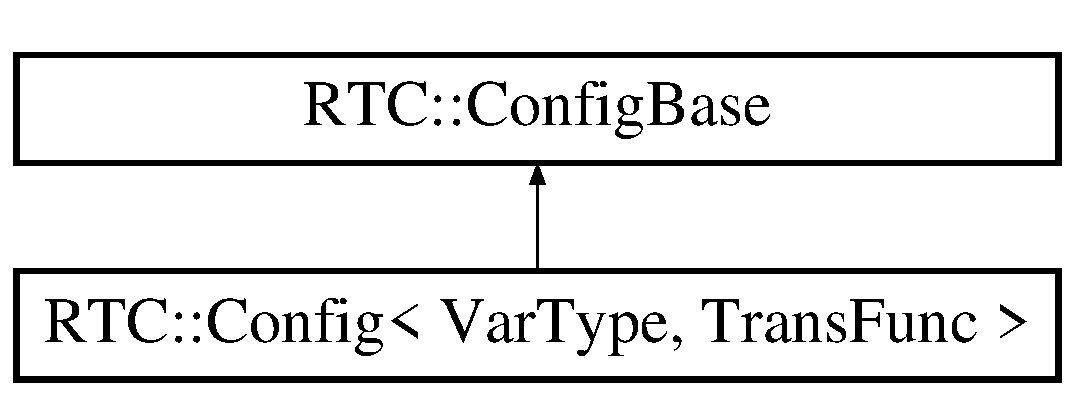
\includegraphics[height=2cm]{classRTC_1_1Config}
\end{center}
\end{figure}
\subsection*{Public メソッド}
\begin{DoxyCompactItemize}
\item 
{\bf Config} (const char $\ast${\bf name}, VarType \&var, const char $\ast$def\_\-val, TransFunc trans=coil::stringTo)
\begin{DoxyCompactList}\small\item\em コンストラクタ \item\end{DoxyCompactList}\item 
virtual {\bf $\sim$Config} (void)
\begin{DoxyCompactList}\small\item\em 仮想デストラクタ \item\end{DoxyCompactList}\item 
virtual bool {\bf update} (const char $\ast$val)
\begin{DoxyCompactList}\small\item\em バインドパラメータ値を更新 \item\end{DoxyCompactList}\end{DoxyCompactItemize}
\subsection*{Protected 変数}
\begin{DoxyCompactItemize}
\item 
VarType \& {\bf m\_\-var}
\begin{DoxyCompactList}\small\item\em コンフィギュレーションパラメータ格納用変数 \item\end{DoxyCompactList}\item 
TransFunc {\bf m\_\-trans}
\begin{DoxyCompactList}\small\item\em コンフィギュレーションパラメータ型文字列変換関数 \item\end{DoxyCompactList}\end{DoxyCompactItemize}


\subsection{説明}
\subsubsection*{template$<$typename VarType, typename TransFunc = bool ($\ast$)(VarType\&, const char$\ast$)$>$ class RTC::Config$<$ VarType, TransFunc $>$}

\doxyref{Config}{p.}{classRTC_1_1Config} クラス. コンフィギュレーションパラメータの情報を保持するクラス。 $<$VarType$>$としてコンフィギュレーションのデータ型を指定する。 $<$TransFunc$>$として設定されたデータ型を文字列に変換する変換関数を 指定する。


\begin{DoxyParams}{引数}
\item[{\em VarType}]コンフィギュレーションパラメータ格納用変数 \item[{\em TransFunc}]格納したデータ型を文字列に変換する変換関数\end{DoxyParams}
\begin{DoxySince}{から}
0.4.0 
\end{DoxySince}


\subsection{コンストラクタとデストラクタ}
\index{RTC::Config@{RTC::Config}!Config@{Config}}
\index{Config@{Config}!RTC::Config@{RTC::Config}}
\subsubsection[{Config}]{\setlength{\rightskip}{0pt plus 5cm}template$<$typename VarType , typename TransFunc  = bool ($\ast$)(VarType\&, const char$\ast$)$>$ {\bf RTC::Config}$<$ VarType, TransFunc $>$::{\bf Config} (const char $\ast$ {\em name}, \/  VarType \& {\em var}, \/  const char $\ast$ {\em def\_\-val}, \/  TransFunc {\em trans} = {\ttfamily coil::stringTo})\hspace{0.3cm}{\ttfamily  [inline]}}\label{classRTC_1_1Config_a5caed5e472c99e525d741ae8fd032d64}


コンストラクタ 

コンストラクタ


\begin{DoxyParams}{引数}
\item[{\em name}]コンフィギュレーションパラメータ名 \item[{\em var}]コンフィギュレーションパラメータ格納用変数 \item[{\em def\_\-val}]文字列形式のデフォルト値 \item[{\em trans}]文字列形式変換関数 \end{DoxyParams}
\index{RTC::Config@{RTC::Config}!$\sim$Config@{$\sim$Config}}
\index{$\sim$Config@{$\sim$Config}!RTC::Config@{RTC::Config}}
\subsubsection[{$\sim$Config}]{\setlength{\rightskip}{0pt plus 5cm}template$<$typename VarType , typename TransFunc  = bool ($\ast$)(VarType\&, const char$\ast$)$>$ virtual {\bf RTC::Config}$<$ VarType, TransFunc $>$::$\sim${\bf Config} (void)\hspace{0.3cm}{\ttfamily  [inline, virtual]}}\label{classRTC_1_1Config_ad0b0e304b1d8746e151cc23441dabf0c}


仮想デストラクタ 

仮想デストラクタ。 

\subsection{関数}
\index{RTC::Config@{RTC::Config}!update@{update}}
\index{update@{update}!RTC::Config@{RTC::Config}}
\subsubsection[{update}]{\setlength{\rightskip}{0pt plus 5cm}template$<$typename VarType , typename TransFunc  = bool ($\ast$)(VarType\&, const char$\ast$)$>$ virtual bool {\bf RTC::Config}$<$ VarType, TransFunc $>$::update (const char $\ast$ {\em val})\hspace{0.3cm}{\ttfamily  [inline, virtual]}}\label{classRTC_1_1Config_ae62b81ad2d80a5f40f594f473f9556fa}


バインドパラメータ値を更新 

コンフィギュレーション設定値でコンフィギュレーションパラメータを更新する


\begin{DoxyParams}{引数}
\item[{\em val}]パラメータ値の文字列表現\end{DoxyParams}
\begin{DoxyReturn}{戻り値}
更新処理結果(更新成功:true,更新失敗:false) 
\end{DoxyReturn}


{\bf RTC::ConfigBase} \doxyref{}{p.}{structRTC_1_1ConfigBase_a353307f47fe534865db2a9173380e38c}を実装しています。



\subsection{変数}
\index{RTC::Config@{RTC::Config}!m\_\-trans@{m\_\-trans}}
\index{m\_\-trans@{m\_\-trans}!RTC::Config@{RTC::Config}}
\subsubsection[{m\_\-trans}]{\setlength{\rightskip}{0pt plus 5cm}template$<$typename VarType , typename TransFunc  = bool ($\ast$)(VarType\&, const char$\ast$)$>$ TransFunc {\bf RTC::Config}$<$ VarType, TransFunc $>$::{\bf m\_\-trans}\hspace{0.3cm}{\ttfamily  [protected]}}\label{classRTC_1_1Config_a944a46727c2b8ed20b1eb92945563658}


コンフィギュレーションパラメータ型文字列変換関数 

\index{RTC::Config@{RTC::Config}!m\_\-var@{m\_\-var}}
\index{m\_\-var@{m\_\-var}!RTC::Config@{RTC::Config}}
\subsubsection[{m\_\-var}]{\setlength{\rightskip}{0pt plus 5cm}template$<$typename VarType , typename TransFunc  = bool ($\ast$)(VarType\&, const char$\ast$)$>$ VarType\& {\bf RTC::Config}$<$ VarType, TransFunc $>$::{\bf m\_\-var}\hspace{0.3cm}{\ttfamily  [protected]}}\label{classRTC_1_1Config_a0ce4e14958ec4d7a45ea8a9aa2e72847}


コンフィギュレーションパラメータ格納用変数 


\section{SDOPackage::Configuration\_\-impl::config\_\-id Struct Reference}
\label{structSDOPackage_1_1Configuration__impl_1_1config__id}\index{SDOPackage::Configuration\_\-impl::config\_\-id@{SDOPackage::Configuration\_\-impl::config\_\-id}}


Functor for ConfigurationSet.  




{\ttfamily \#include $<$SdoConfiguration.h$>$}

\subsection*{Public Member Functions}
\begin{DoxyCompactItemize}
\item 
{\bf config\_\-id} (const char $\ast$id)
\item 
bool {\bf operator()} (const ConfigurationSet \&c)
\end{DoxyCompactItemize}
\subsection*{Public Attributes}
\begin{DoxyCompactItemize}
\item 
const std::string {\bf m\_\-id}
\end{DoxyCompactItemize}


\subsection{Detailed Description}
Functor for ConfigurationSet. 

\subsection{Constructor \& Destructor Documentation}
\index{SDOPackage::Configuration\_\-impl::config\_\-id@{SDOPackage::Configuration\_\-impl::config\_\-id}!config\_\-id@{config\_\-id}}
\index{config\_\-id@{config\_\-id}!SDOPackage::Configuration_impl::config_id@{SDOPackage::Configuration\_\-impl::config\_\-id}}
\subsubsection[{config\_\-id}]{\setlength{\rightskip}{0pt plus 5cm}SDOPackage::Configuration\_\-impl::config\_\-id::config\_\-id (const char $\ast$ {\em id})\hspace{0.3cm}{\ttfamily  [inline]}}\label{structSDOPackage_1_1Configuration__impl_1_1config__id_a5a00969e9d9c016597921bdab51db000}


\subsection{Member Function Documentation}
\index{SDOPackage::Configuration\_\-impl::config\_\-id@{SDOPackage::Configuration\_\-impl::config\_\-id}!operator()@{operator()}}
\index{operator()@{operator()}!SDOPackage::Configuration_impl::config_id@{SDOPackage::Configuration\_\-impl::config\_\-id}}
\subsubsection[{operator()}]{\setlength{\rightskip}{0pt plus 5cm}bool SDOPackage::Configuration\_\-impl::config\_\-id::operator() (const ConfigurationSet \& {\em c})\hspace{0.3cm}{\ttfamily  [inline]}}\label{structSDOPackage_1_1Configuration__impl_1_1config__id_a94108b7a0dd16322a000373b84d3311f}


References m\_\-id.



\subsection{Member Data Documentation}
\index{SDOPackage::Configuration\_\-impl::config\_\-id@{SDOPackage::Configuration\_\-impl::config\_\-id}!m\_\-id@{m\_\-id}}
\index{m\_\-id@{m\_\-id}!SDOPackage::Configuration_impl::config_id@{SDOPackage::Configuration\_\-impl::config\_\-id}}
\subsubsection[{m\_\-id}]{\setlength{\rightskip}{0pt plus 5cm}const std::string {\bf SDOPackage::Configuration\_\-impl::config\_\-id::m\_\-id}}\label{structSDOPackage_1_1Configuration__impl_1_1config__id_acff37c9e605b6bc7b7345b96d8202fc4}


Referenced by operator()().


\section{クラス RTC::ConfigAdmin}
\label{classRTC_1_1ConfigAdmin}\index{RTC::ConfigAdmin@{RTC::ConfigAdmin}}


\doxyref{ConfigAdmin}{p.}{classRTC_1_1ConfigAdmin} クラス.  




{\ttfamily \#include $<$ConfigAdmin.h$>$}

\subsection*{構成}
\begin{DoxyCompactItemize}
\item 
struct {\bfseries find\_\-conf}
\end{DoxyCompactItemize}
\subsection*{Public メソッド}
\begin{DoxyCompactItemize}
\item 
{\bf ConfigAdmin} ({\bf coil::Properties} \&prop)
\begin{DoxyCompactList}\small\item\em コンストラクタ \item\end{DoxyCompactList}\item 
{\bf $\sim$ConfigAdmin} (void)
\begin{DoxyCompactList}\small\item\em 仮想デストラクタ \item\end{DoxyCompactList}\item 
{\footnotesize template$<$typename VarType $>$ }\\bool {\bf bindParameter} (const char $\ast$param\_\-name, VarType \&var, const char $\ast$def\_\-val, bool($\ast$trans)(VarType \&, const char $\ast$)=coil::stringTo)
\begin{DoxyCompactList}\small\item\em コンフィギュレーションパラメータの設定 \item\end{DoxyCompactList}\item 
void {\bf update} (void)
\begin{DoxyCompactList}\small\item\em コンフィギュレーションパラメータの更新 (アクティブコンフィギュレーションセット) \item\end{DoxyCompactList}\item 
void {\bf update} (const char $\ast$config\_\-set)
\begin{DoxyCompactList}\small\item\em コンフィギュレーションパラメータの更新(ID指定) \item\end{DoxyCompactList}\item 
void {\bf update} (const char $\ast$config\_\-set, const char $\ast$config\_\-param)
\begin{DoxyCompactList}\small\item\em コンフィギュレーションパラメータの更新(名称指定) \item\end{DoxyCompactList}\item 
bool {\bf isExist} (const char $\ast$name)
\begin{DoxyCompactList}\small\item\em コンフィギュレーションパラメータの存在確認 \item\end{DoxyCompactList}\item 
bool {\bf isChanged} (void)
\begin{DoxyCompactList}\small\item\em コンフィギュレーションパラメータの変更確認 \item\end{DoxyCompactList}\item 
const char $\ast$ {\bf getActiveId} (void)
\begin{DoxyCompactList}\small\item\em アクティブ・コンフィギュレーションセットIDの取得 \item\end{DoxyCompactList}\item 
bool {\bf haveConfig} (const char $\ast$config\_\-id)
\begin{DoxyCompactList}\small\item\em コンフィギュレーションセットの存在確認 \item\end{DoxyCompactList}\item 
bool {\bf isActive} (void)
\begin{DoxyCompactList}\small\item\em コンフィギュレーションセットのアクティブ化確認 \item\end{DoxyCompactList}\item 
const std::vector$<$ {\bf coil::Properties} $\ast$ $>$ \& {\bf getConfigurationSets} (void)
\begin{DoxyCompactList}\small\item\em 全コンフィギュレーションセットの取得 \item\end{DoxyCompactList}\item 
const {\bf coil::Properties} \& {\bf getConfigurationSet} (const char $\ast$config\_\-id)
\begin{DoxyCompactList}\small\item\em 指定したIDのコンフィギュレーションセットの取得 \item\end{DoxyCompactList}\item 
bool {\bf setConfigurationSetValues} (const {\bf coil::Properties} \&configuration\_\-set)
\begin{DoxyCompactList}\small\item\em 指定したプロパティのコンフィギュレーションセットへの追加 \item\end{DoxyCompactList}\item 
const {\bf coil::Properties} \& {\bf getActiveConfigurationSet} (void)
\begin{DoxyCompactList}\small\item\em アクティブ・コンフィギュレーションセットを取得 \item\end{DoxyCompactList}\item 
bool {\bf addConfigurationSet} (const {\bf coil::Properties} \&configuration\_\-set)
\begin{DoxyCompactList}\small\item\em コンフィギュレーションセットに設定値を追加 \item\end{DoxyCompactList}\item 
bool {\bf removeConfigurationSet} (const char $\ast$config\_\-id)
\begin{DoxyCompactList}\small\item\em コンフィギュレーションセットの削除 \item\end{DoxyCompactList}\item 
bool {\bf activateConfigurationSet} (const char $\ast$config\_\-id)
\begin{DoxyCompactList}\small\item\em コンフィギュレーションセットのアクティブ化 \item\end{DoxyCompactList}\item 
void {\bf setOnUpdate} ({\bf OnUpdateCallback} $\ast$cb)
\item 
void {\bf setOnUpdateParam} ({\bf OnUpdateParamCallback} $\ast$cb)
\item 
void {\bf setOnSetConfigurationSet} ({\bf OnSetConfigurationSetCallback} $\ast$cb)
\item 
void {\bf setOnAddConfigurationSet} ({\bf OnAddConfigurationAddCallback} $\ast$cb)
\item 
void {\bf setOnRemoveConfigurationSet} ({\bf OnRemoveConfigurationSetCallback} $\ast$cb)
\item 
void {\bf setOnActivateSet} ({\bf OnActivateSetCallback} $\ast$cb)
\item 
void {\bf addConfigurationParamListener} ({\bf ConfigurationParamListenerType} type, {\bf ConfigurationParamListener} $\ast$listener, bool autoclean=true)
\begin{DoxyCompactList}\small\item\em \doxyref{ConfigurationParamListener}{p.}{classRTC_1_1ConfigurationParamListener} を追加する. \item\end{DoxyCompactList}\item 
void {\bf removeConfigurationParamListener} ({\bf ConfigurationParamListenerType} type, {\bf ConfigurationParamListener} $\ast$listener)
\begin{DoxyCompactList}\small\item\em \doxyref{ConfigurationParamListener}{p.}{classRTC_1_1ConfigurationParamListener} を削除する. \item\end{DoxyCompactList}\item 
void {\bf addConfigurationSetListener} ({\bf ConfigurationSetListenerType} type, {\bf ConfigurationSetListener} $\ast$listener, bool autoclean=true)
\begin{DoxyCompactList}\small\item\em \doxyref{ConfigurationSetListener}{p.}{classRTC_1_1ConfigurationSetListener} を追加する. \item\end{DoxyCompactList}\item 
void {\bf removeConfigurationSetListener} ({\bf ConfigurationSetListenerType} type, {\bf ConfigurationSetListener} $\ast$listener)
\begin{DoxyCompactList}\small\item\em \doxyref{ConfigurationSetListener}{p.}{classRTC_1_1ConfigurationSetListener} を削除する. \item\end{DoxyCompactList}\item 
void {\bf addConfigurationSetNameListener} ({\bf ConfigurationSetNameListenerType} type, {\bf ConfigurationSetNameListener} $\ast$listener, bool autoclean=true)
\begin{DoxyCompactList}\small\item\em \doxyref{ConfigurationSetNameListener}{p.}{classRTC_1_1ConfigurationSetNameListener} を追加する. \item\end{DoxyCompactList}\item 
void {\bf removeConfigurationSetNameListener} ({\bf ConfigurationSetNameListenerType} type, {\bf ConfigurationSetNameListener} $\ast$listener)
\begin{DoxyCompactList}\small\item\em \doxyref{ConfigurationSetNameListener}{p.}{classRTC_1_1ConfigurationSetNameListener} を削除する. \item\end{DoxyCompactList}\end{DoxyCompactItemize}
\subsection*{Protected メソッド}
\begin{DoxyCompactItemize}
\item 
void {\bf onUpdate} (const char $\ast$config\_\-set)
\begin{DoxyCompactList}\small\item\em コンフィギュレーションパラメータの更新(ID指定)時にコールされる \item\end{DoxyCompactList}\item 
void {\bf onUpdateParam} (const char $\ast$config\_\-set, const char $\ast$config\_\-param)
\begin{DoxyCompactList}\small\item\em コンフィギュレーションパラメータの更新(名称指定)時にコールされる \item\end{DoxyCompactList}\item 
void {\bf onSetConfigurationSet} (const {\bf coil::Properties} \&config\_\-set)
\begin{DoxyCompactList}\small\item\em コンフィギュレーションセットへの追加時にコールされる \item\end{DoxyCompactList}\item 
void {\bf onAddConfigurationSet} (const {\bf coil::Properties} \&config\_\-set)
\begin{DoxyCompactList}\small\item\em 設定値が追加されたときにコールされる。 \item\end{DoxyCompactList}\item 
void {\bf onRemoveConfigurationSet} (const char $\ast$config\_\-id)
\begin{DoxyCompactList}\small\item\em セットが削除されてるときにコールされる。 \item\end{DoxyCompactList}\item 
void {\bf onActivateSet} (const char $\ast$config\_\-id)
\begin{DoxyCompactList}\small\item\em セットがアクティブ化されたときにコールされる。 \item\end{DoxyCompactList}\end{DoxyCompactItemize}


\subsection{説明}
\doxyref{ConfigAdmin}{p.}{classRTC_1_1ConfigAdmin} クラス. 各種コンフィギュレーション情報を管理するクラス。 用語を以下のように定義する。


\begin{DoxyItemize}
\item コンフィギュレーション: コンポーネントの設定情報。
\end{DoxyItemize}


\begin{DoxyItemize}
\item (コンフィギュレーション)パラメータ: key-\/value からなる設定情報。 \doxyref{coil::Properties}{p.}{classcoil_1_1Properties} 変数として扱われ、key、value 共に文字列として保 持される。key をコンフィギュレーションパラメータ名、value をコン フィギュレーションパラメータ値と呼ぶ。
\end{DoxyItemize}


\begin{DoxyItemize}
\item コンフィギュレーションセット: コンフィギュレーションパラメータ のリストで、名前 (ID) によって区別される。IDをコンフィギュレーショ ンセットIDと呼ぶ。
\end{DoxyItemize}


\begin{DoxyItemize}
\item (コンフィギュレーション)パラメータ変数:コンフィギュレーションパ ラメータをRTCのアクティビティ内で実際に利用する際に参照される変 数。パラメータごとに固有の型を持つ。
\end{DoxyItemize}


\begin{DoxyItemize}
\item アクティブ(コンフィギュレーション)セット:現在有効なコンフィギュ レーションセットのことであり、唯一つ存在する。原則として、アクティ ブコンフィギュレーションセットのパラメータがコンフィギュレーショ ンパラメータ変数に反映される。
\end{DoxyItemize}

このクラスでは、コンフィギュレーションのための以下の2つの情報を保 持している。


\begin{DoxyEnumerate}
\item コンフィギュレーションセットのリスト
\item パラメータ変数のリスト
\end{DoxyEnumerate}

基本的には、(1) のコンフィギュレーションセットのリストのうち一つを、 (2) のパラメータ変数へ反映させる、のが本クラスの目的である。通常、 パラメータ変数の変更操作は、コンフィギュレーションセットの変更とパ ラメータ変数への反映の2段階で行われる。

コンフィギュレーションセットのリストの操作には、以下の関数を用いる。


\begin{DoxyItemize}
\item \doxyref{getConfigurationSets()}{p.}{classRTC_1_1ConfigAdmin_a9367d39f878ec8d817e8aabacd27deb6}
\item \doxyref{getConfigurationSet()}{p.}{classRTC_1_1ConfigAdmin_a51b2ad46ba5184fc1361dbd86ed2309a}
\item \doxyref{setConfigurationSetValues()}{p.}{classRTC_1_1ConfigAdmin_a31d4e545b48aa3ea2fc03109b301586d}
\item \doxyref{getActiveConfigurationSet()}{p.}{classRTC_1_1ConfigAdmin_a40c1de78caa9c8ff2ca02ee972f26bb9}
\item \doxyref{addConfigurationSet()}{p.}{classRTC_1_1ConfigAdmin_a35e38434ba8b409ae1207d81f4904a4d}
\item \doxyref{removeConfigurationSet()}{p.}{classRTC_1_1ConfigAdmin_aef99fcfb1f6ca7b09b85c10082236f71}
\item \doxyref{activateConfigurationSet()}{p.}{classRTC_1_1ConfigAdmin_a5215efd13ca14ed67cbbbd533556c0a3}
\end{DoxyItemize}

これらの関数により、コンフィギュレーションセットの変更、追加、削除、 取得、アクティブ化を行う。これらの操作により変更されたコンフィギュ レーションセットを、RTCのアクティビティから使用するパラメータ変数 に反映させるには、以下の \doxyref{update()}{p.}{classRTC_1_1ConfigAdmin_a858c419de43392804dd934dd62c1874a} 関数を用いる。


\begin{DoxyItemize}
\item \doxyref{update(void)}{p.}{classRTC_1_1ConfigAdmin_a858c419de43392804dd934dd62c1874a}
\item \doxyref{update(const char$\ast$ config\_\-set)}{p.}{classRTC_1_1ConfigAdmin_a6a183d22dfa7c58ba5d21982aac34645}
\item \doxyref{update(const char$\ast$ config\_\-set, const char$\ast$ config\_\-param)}{p.}{classRTC_1_1ConfigAdmin_a4b1ce69c995d6a89d743cbfd38088de4}
\end{DoxyItemize}

コンフィギュレーション操作をフックするためにコールバックファンクタ を与えることができる。フックできる操作は以下の通り。


\begin{DoxyItemize}
\item ON\_\-UPDATE : \doxyref{update()}{p.}{classRTC_1_1ConfigAdmin_a858c419de43392804dd934dd62c1874a} コール時
\item ON\_\-UPDATE\_\-PARAM : update(param) コール時
\item ON\_\-SET\_\-CONFIGURATIONSET : setConfigurationSet() コール時
\item ON\_\-ADD\_\-CONFIGURATIONSET : \doxyref{addConfigurationSet()}{p.}{classRTC_1_1ConfigAdmin_a35e38434ba8b409ae1207d81f4904a4d} コール時
\item ON\_\-REMOVE\_\-CONFIGURATIONSET : \doxyref{removeConfigurationSet()}{p.}{classRTC_1_1ConfigAdmin_aef99fcfb1f6ca7b09b85c10082236f71} コール時
\item ON\_\-ACTIVATE\_\-CONFIGURATIONSET: \doxyref{activateConfigurationSet()}{p.}{classRTC_1_1ConfigAdmin_a5215efd13ca14ed67cbbbd533556c0a3} コール時
\end{DoxyItemize}

\begin{DoxySince}{から}
0.4.0 
\end{DoxySince}


\subsection{コンストラクタとデストラクタ}
\index{RTC::ConfigAdmin@{RTC::ConfigAdmin}!ConfigAdmin@{ConfigAdmin}}
\index{ConfigAdmin@{ConfigAdmin}!RTC::ConfigAdmin@{RTC::ConfigAdmin}}
\subsubsection[{ConfigAdmin}]{\setlength{\rightskip}{0pt plus 5cm}RTC::ConfigAdmin::ConfigAdmin ({\bf coil::Properties} \& {\em prop})}\label{classRTC_1_1ConfigAdmin_a28596cf49170b6e982ffcb9d6046eb2b}


コンストラクタ 

コンストラクタ


\begin{DoxyParams}{引数}
\item[{\em prop}]設定対象プロパティ名 \end{DoxyParams}
\index{RTC::ConfigAdmin@{RTC::ConfigAdmin}!$\sim$ConfigAdmin@{$\sim$ConfigAdmin}}
\index{$\sim$ConfigAdmin@{$\sim$ConfigAdmin}!RTC::ConfigAdmin@{RTC::ConfigAdmin}}
\subsubsection[{$\sim$ConfigAdmin}]{\setlength{\rightskip}{0pt plus 5cm}RTC::ConfigAdmin::$\sim$ConfigAdmin (void)}\label{classRTC_1_1ConfigAdmin_a95583c13525f3dde969248f1ae68624d}


仮想デストラクタ 

仮想デストラクタ。 

\subsection{関数}
\index{RTC::ConfigAdmin@{RTC::ConfigAdmin}!activateConfigurationSet@{activateConfigurationSet}}
\index{activateConfigurationSet@{activateConfigurationSet}!RTC::ConfigAdmin@{RTC::ConfigAdmin}}
\subsubsection[{activateConfigurationSet}]{\setlength{\rightskip}{0pt plus 5cm}bool RTC::ConfigAdmin::activateConfigurationSet (const char $\ast$ {\em config\_\-id})}\label{classRTC_1_1ConfigAdmin_a5215efd13ca14ed67cbbbd533556c0a3}


コンフィギュレーションセットのアクティブ化 

指定したIDのコンフィギュレーションセットをアクティブ化する。 指定したIDのコンフィギュレーションセットが存在しない場合は、 falseを返す。


\begin{DoxyParams}{引数}
\item[{\em config\_\-id}]削除対象コンフィギュレーションセットのID\end{DoxyParams}
\begin{DoxyReturn}{戻り値}
アクティブ処理結果(成功:true、失敗:false) 
\end{DoxyReturn}
\index{RTC::ConfigAdmin@{RTC::ConfigAdmin}!addConfigurationParamListener@{addConfigurationParamListener}}
\index{addConfigurationParamListener@{addConfigurationParamListener}!RTC::ConfigAdmin@{RTC::ConfigAdmin}}
\subsubsection[{addConfigurationParamListener}]{\setlength{\rightskip}{0pt plus 5cm}void RTC::ConfigAdmin::addConfigurationParamListener ({\bf ConfigurationParamListenerType} {\em type}, \/  {\bf ConfigurationParamListener} $\ast$ {\em listener}, \/  bool {\em autoclean} = {\ttfamily true})}\label{classRTC_1_1ConfigAdmin_a8cb21913dd1346a4f0780f9bd242489e}


\doxyref{ConfigurationParamListener}{p.}{classRTC_1_1ConfigurationParamListener} を追加する. 

\doxyref{update(const char$\ast$ config\_\-set, const char$\ast$ config\_\-param)}{p.}{classRTC_1_1ConfigAdmin_a4b1ce69c995d6a89d743cbfd38088de4} が呼ばれた際に コールされるリスナ \doxyref{ConfigurationParamListener}{p.}{classRTC_1_1ConfigurationParamListener} を追加する。 type には現在のところ ON\_\-UPDATE\_\-CONFIG\_\-PARAM のみが入る。


\begin{DoxyParams}{引数}
\item[{\em type}]ConfigurationParamListenerType型の値。 ON\_\-UPDATE\_\-CONFIG\_\-PARAM がある。\item[{\em listener}]\doxyref{ConfigurationParamListener}{p.}{classRTC_1_1ConfigurationParamListener} 型のリスナオブジェクト。 \item[{\em autoclean}]リスナオブジェクトを自動で削除するかどうかのフラグ \end{DoxyParams}
\index{RTC::ConfigAdmin@{RTC::ConfigAdmin}!addConfigurationSet@{addConfigurationSet}}
\index{addConfigurationSet@{addConfigurationSet}!RTC::ConfigAdmin@{RTC::ConfigAdmin}}
\subsubsection[{addConfigurationSet}]{\setlength{\rightskip}{0pt plus 5cm}bool RTC::ConfigAdmin::addConfigurationSet (const {\bf coil::Properties} \& {\em configuration\_\-set})}\label{classRTC_1_1ConfigAdmin_a35e38434ba8b409ae1207d81f4904a4d}


コンフィギュレーションセットに設定値を追加 

コンフィギュレーションセットに設定値を追加する。


\begin{DoxyParams}{引数}
\item[{\em configuration\_\-set}]追加するプロパティ\end{DoxyParams}
\begin{DoxyReturn}{戻り値}
追加処理結果(追加成功:true、追加失敗:false) 
\end{DoxyReturn}
\index{RTC::ConfigAdmin@{RTC::ConfigAdmin}!addConfigurationSetListener@{addConfigurationSetListener}}
\index{addConfigurationSetListener@{addConfigurationSetListener}!RTC::ConfigAdmin@{RTC::ConfigAdmin}}
\subsubsection[{addConfigurationSetListener}]{\setlength{\rightskip}{0pt plus 5cm}void RTC::ConfigAdmin::addConfigurationSetListener ({\bf ConfigurationSetListenerType} {\em type}, \/  {\bf ConfigurationSetListener} $\ast$ {\em listener}, \/  bool {\em autoclean} = {\ttfamily true})}\label{classRTC_1_1ConfigAdmin_ab230e41c008e759111274ba4a6002e1b}


\doxyref{ConfigurationSetListener}{p.}{classRTC_1_1ConfigurationSetListener} を追加する. 

ConfigurationSet が更新されたときなどに呼ばれるリスナ \doxyref{ConfigurationSetListener}{p.}{classRTC_1_1ConfigurationSetListener} を追加する。設定可能なイベントは以下の 2種類がある。


\begin{DoxyItemize}
\item ON\_\-SET\_\-CONFIG\_\-SET: \doxyref{setConfigurationSetValues()}{p.}{classRTC_1_1ConfigAdmin_a31d4e545b48aa3ea2fc03109b301586d} で ConfigurationSet に値が設定された場合。
\item ON\_\-ADD\_\-CONFIG\_\-SET: \doxyref{addConfigurationSet()}{p.}{classRTC_1_1ConfigAdmin_a35e38434ba8b409ae1207d81f4904a4d} で新しい ConfigurationSet が追加された場合。
\end{DoxyItemize}


\begin{DoxyParams}{引数}
\item[{\em type}]ConfigurationSetListenerType型の値。 \item[{\em listener}]\doxyref{ConfigurationSetListener}{p.}{classRTC_1_1ConfigurationSetListener} 型のリスナオブジェクト。 \item[{\em autoclean}]リスナオブジェクトを自動で削除するかどうかのフラグ \end{DoxyParams}
\index{RTC::ConfigAdmin@{RTC::ConfigAdmin}!addConfigurationSetNameListener@{addConfigurationSetNameListener}}
\index{addConfigurationSetNameListener@{addConfigurationSetNameListener}!RTC::ConfigAdmin@{RTC::ConfigAdmin}}
\subsubsection[{addConfigurationSetNameListener}]{\setlength{\rightskip}{0pt plus 5cm}void RTC::ConfigAdmin::addConfigurationSetNameListener ({\bf ConfigurationSetNameListenerType} {\em type}, \/  {\bf ConfigurationSetNameListener} $\ast$ {\em listener}, \/  bool {\em autoclean} = {\ttfamily true})}\label{classRTC_1_1ConfigAdmin_acb37502f739689a2a9679c4124cf7e13}


\doxyref{ConfigurationSetNameListener}{p.}{classRTC_1_1ConfigurationSetNameListener} を追加する. 

ConfigurationSetName が更新されたときなどに呼ばれるリスナ \doxyref{ConfigurationSetNameListener}{p.}{classRTC_1_1ConfigurationSetNameListener} を追加する。設定可能なイベントは以下の 3種類がある。


\begin{DoxyItemize}
\item ON\_\-UPDATE\_\-CONFIG\_\-SET: ある ConfigurationSet がアップデートされた
\item ON\_\-REMOVE\_\-CONFIG\_\-SET: ある ConfigurationSet が削除された
\item ON\_\-ACTIVATE\_\-CONFIG\_\-SET: ある ConfigurationSet がアクティブ化された
\end{DoxyItemize}


\begin{DoxyParams}{引数}
\item[{\em type}]ConfigurationSetNameListenerType型の値。 \item[{\em listener}]\doxyref{ConfigurationSetNameListener}{p.}{classRTC_1_1ConfigurationSetNameListener} 型のリスナオブジェクト。 \item[{\em autoclean}]リスナオブジェクトを自動で削除するかどうかのフラグ \end{DoxyParams}
\index{RTC::ConfigAdmin@{RTC::ConfigAdmin}!bindParameter@{bindParameter}}
\index{bindParameter@{bindParameter}!RTC::ConfigAdmin@{RTC::ConfigAdmin}}
\subsubsection[{bindParameter}]{\setlength{\rightskip}{0pt plus 5cm}template$<$typename VarType $>$ bool RTC::ConfigAdmin::bindParameter (const char $\ast$ {\em param\_\-name}, \/  VarType \& {\em var}, \/  const char $\ast$ {\em def\_\-val}, \/  bool($\ast$)(VarType \&, const char $\ast$) {\em trans} = {\ttfamily coil::stringTo})\hspace{0.3cm}{\ttfamily  [inline]}}\label{classRTC_1_1ConfigAdmin_a2c1674931ce1cff6815df69f2a7a3a7c}


コンフィギュレーションパラメータの設定 

コンフィギュレーションパラメータと変数をバインドする 指定した名称のコンフィギュレーションパラメータが既に存在する場合は falseを返す。 $<$VarType$>$としてコンフィギュレーションパラメータのデータ型を指定する。


\begin{DoxyParams}{引数}
\item[{\em param\_\-name}]コンフィギュレーションパラメータ名 \item[{\em var}]コンフィギュレーションパラメータ格納用変数 \item[{\em def\_\-val}]コンフィギュレーションパラメータデフォルト値 \item[{\em trans}]コンフィギュレーションパラメータ文字列変換用関数\end{DoxyParams}
\begin{DoxyReturn}{戻り値}
設定結果(設定成功:true,設定失敗:false) 
\end{DoxyReturn}


参照元 RTC::RTObject\_\-impl::bindParameter().

\index{RTC::ConfigAdmin@{RTC::ConfigAdmin}!getActiveConfigurationSet@{getActiveConfigurationSet}}
\index{getActiveConfigurationSet@{getActiveConfigurationSet}!RTC::ConfigAdmin@{RTC::ConfigAdmin}}
\subsubsection[{getActiveConfigurationSet}]{\setlength{\rightskip}{0pt plus 5cm}const {\bf coil::Properties}\& RTC::ConfigAdmin::getActiveConfigurationSet (void)}\label{classRTC_1_1ConfigAdmin_a40c1de78caa9c8ff2ca02ee972f26bb9}


アクティブ・コンフィギュレーションセットを取得 

現在アクティブとなっているコンフィギュレーションセットを取得する。 アクティブとなっているコンフィギュレーションセットが存在しない場合は、 空のコンフィギュレーションセット を返す。

\begin{DoxyReturn}{戻り値}
アクティブ・コンフィギュレーションセット 
\end{DoxyReturn}
\index{RTC::ConfigAdmin@{RTC::ConfigAdmin}!getActiveId@{getActiveId}}
\index{getActiveId@{getActiveId}!RTC::ConfigAdmin@{RTC::ConfigAdmin}}
\subsubsection[{getActiveId}]{\setlength{\rightskip}{0pt plus 5cm}const char$\ast$ RTC::ConfigAdmin::getActiveId (void)\hspace{0.3cm}{\ttfamily  [inline]}}\label{classRTC_1_1ConfigAdmin_a54b5645d445e5b0670ed959f8a7d0f91}


アクティブ・コンフィギュレーションセットIDの取得 

現在アクティブなコンフィギュレーションセットのIDを取得する。

\begin{DoxyReturn}{戻り値}
アクティブ・コンフィギュレーションセットID 
\end{DoxyReturn}
\index{RTC::ConfigAdmin@{RTC::ConfigAdmin}!getConfigurationSet@{getConfigurationSet}}
\index{getConfigurationSet@{getConfigurationSet}!RTC::ConfigAdmin@{RTC::ConfigAdmin}}
\subsubsection[{getConfigurationSet}]{\setlength{\rightskip}{0pt plus 5cm}const {\bf coil::Properties}\& RTC::ConfigAdmin::getConfigurationSet (const char $\ast$ {\em config\_\-id})}\label{classRTC_1_1ConfigAdmin_a51b2ad46ba5184fc1361dbd86ed2309a}


指定したIDのコンフィギュレーションセットの取得 

IDで指定したコンフィギュレーションセットを取得する。 指定したコンフィギュレーションセットが存在しない場合は、 空のコンフィギュレーションセットを返す。


\begin{DoxyParams}{引数}
\item[{\em config\_\-id}]取得対象コンフィギュレーションセットのID\end{DoxyParams}
\begin{DoxyReturn}{戻り値}
コンフィギュレーションセット 
\end{DoxyReturn}
\index{RTC::ConfigAdmin@{RTC::ConfigAdmin}!getConfigurationSets@{getConfigurationSets}}
\index{getConfigurationSets@{getConfigurationSets}!RTC::ConfigAdmin@{RTC::ConfigAdmin}}
\subsubsection[{getConfigurationSets}]{\setlength{\rightskip}{0pt plus 5cm}const std::vector$<${\bf coil::Properties}$\ast$$>$\& RTC::ConfigAdmin::getConfigurationSets (void)}\label{classRTC_1_1ConfigAdmin_a9367d39f878ec8d817e8aabacd27deb6}


全コンフィギュレーションセットの取得 

設定されている全コンフィギュレーションセットを取得する。

\begin{DoxyReturn}{戻り値}
全コンフィギュレーションセット 
\end{DoxyReturn}
\index{RTC::ConfigAdmin@{RTC::ConfigAdmin}!haveConfig@{haveConfig}}
\index{haveConfig@{haveConfig}!RTC::ConfigAdmin@{RTC::ConfigAdmin}}
\subsubsection[{haveConfig}]{\setlength{\rightskip}{0pt plus 5cm}bool RTC::ConfigAdmin::haveConfig (const char $\ast$ {\em config\_\-id})\hspace{0.3cm}{\ttfamily  [inline]}}\label{classRTC_1_1ConfigAdmin_ae9f137786d647ff991566def5b5a755c}


コンフィギュレーションセットの存在確認 

指定したコンフィギュレーションセットが存在するか確認する。


\begin{DoxyParams}{引数}
\item[{\em config\_\-id}]確認対象コンフィギュレーションセットID\end{DoxyParams}
\begin{DoxyReturn}{戻り値}
存在確認結果(指定したConfigSetあり:true、なし:false) 
\end{DoxyReturn}
\index{RTC::ConfigAdmin@{RTC::ConfigAdmin}!isActive@{isActive}}
\index{isActive@{isActive}!RTC::ConfigAdmin@{RTC::ConfigAdmin}}
\subsubsection[{isActive}]{\setlength{\rightskip}{0pt plus 5cm}bool RTC::ConfigAdmin::isActive (void)\hspace{0.3cm}{\ttfamily  [inline]}}\label{classRTC_1_1ConfigAdmin_aa040caf9bf2b2970d90e779694144cb6}


コンフィギュレーションセットのアクティブ化確認 

コンフィギュレーションセットがアクティブ化されているか確認する。

\begin{DoxyReturn}{戻り値}
状態確認結果(アクティブ状態:true、非アクティブ状態:false) 
\end{DoxyReturn}
\index{RTC::ConfigAdmin@{RTC::ConfigAdmin}!isChanged@{isChanged}}
\index{isChanged@{isChanged}!RTC::ConfigAdmin@{RTC::ConfigAdmin}}
\subsubsection[{isChanged}]{\setlength{\rightskip}{0pt plus 5cm}bool RTC::ConfigAdmin::isChanged (void)\hspace{0.3cm}{\ttfamily  [inline]}}\label{classRTC_1_1ConfigAdmin_a455bea81a5322f75b578d0f727eda59b}


コンフィギュレーションパラメータの変更確認 

コンフィギュレーションパラメータが変更されたか確認する。

\begin{DoxyReturn}{戻り値}
変更確認結果(変更あり:true、変更なし:false) 
\end{DoxyReturn}
\index{RTC::ConfigAdmin@{RTC::ConfigAdmin}!isExist@{isExist}}
\index{isExist@{isExist}!RTC::ConfigAdmin@{RTC::ConfigAdmin}}
\subsubsection[{isExist}]{\setlength{\rightskip}{0pt plus 5cm}bool RTC::ConfigAdmin::isExist (const char $\ast$ {\em name})}\label{classRTC_1_1ConfigAdmin_ab831318a81892b36a1b9ffeff5d94f52}


コンフィギュレーションパラメータの存在確認 

指定した名称を持つコンフィギュレーションパラメータ変数が存在する か確認する。ここで存在確認を行うパラメータ変数とは、 \doxyref{bindParameter()}{p.}{classRTC_1_1ConfigAdmin_a2c1674931ce1cff6815df69f2a7a3a7c} によって登録される、変数を持つパラメータである。


\begin{DoxyParams}{引数}
\item[{\em name}]コンフィギュレーションパラメータ名称。\end{DoxyParams}
\begin{DoxyReturn}{戻り値}
存在確認結果(パラメータあり:true,パラメータなし:false) 
\end{DoxyReturn}
\index{RTC::ConfigAdmin@{RTC::ConfigAdmin}!onActivateSet@{onActivateSet}}
\index{onActivateSet@{onActivateSet}!RTC::ConfigAdmin@{RTC::ConfigAdmin}}
\subsubsection[{onActivateSet}]{\setlength{\rightskip}{0pt plus 5cm}void RTC::ConfigAdmin::onActivateSet (const char $\ast$ {\em config\_\-id})\hspace{0.3cm}{\ttfamily  [protected]}}\label{classRTC_1_1ConfigAdmin_ace61d4e3f1c644c1ffb8151807fdd76d}


セットがアクティブ化されたときにコールされる。 

設定されてるコールバックオブジェクトを呼び出す。


\begin{DoxyParams}{引数}
\item[{\em config\_\-id}]プロパティ \end{DoxyParams}
\index{RTC::ConfigAdmin@{RTC::ConfigAdmin}!onAddConfigurationSet@{onAddConfigurationSet}}
\index{onAddConfigurationSet@{onAddConfigurationSet}!RTC::ConfigAdmin@{RTC::ConfigAdmin}}
\subsubsection[{onAddConfigurationSet}]{\setlength{\rightskip}{0pt plus 5cm}void RTC::ConfigAdmin::onAddConfigurationSet (const {\bf coil::Properties} \& {\em config\_\-set})\hspace{0.3cm}{\ttfamily  [protected]}}\label{classRTC_1_1ConfigAdmin_aabb91b474ddf417b91b6c61c65ff06f0}


設定値が追加されたときにコールされる。 

設定されてるコールバックオブジェクトを呼び出す。


\begin{DoxyParams}{引数}
\item[{\em configuration\_\-set}]プロパティ \end{DoxyParams}
\index{RTC::ConfigAdmin@{RTC::ConfigAdmin}!onRemoveConfigurationSet@{onRemoveConfigurationSet}}
\index{onRemoveConfigurationSet@{onRemoveConfigurationSet}!RTC::ConfigAdmin@{RTC::ConfigAdmin}}
\subsubsection[{onRemoveConfigurationSet}]{\setlength{\rightskip}{0pt plus 5cm}void RTC::ConfigAdmin::onRemoveConfigurationSet (const char $\ast$ {\em config\_\-id})\hspace{0.3cm}{\ttfamily  [protected]}}\label{classRTC_1_1ConfigAdmin_aab440a6cf5e8562a54834aa7697007c1}


セットが削除されてるときにコールされる。 

設定されてるコールバックオブジェクトを呼び出す。


\begin{DoxyParams}{引数}
\item[{\em config\_\-id}]プロパティ \end{DoxyParams}
\index{RTC::ConfigAdmin@{RTC::ConfigAdmin}!onSetConfigurationSet@{onSetConfigurationSet}}
\index{onSetConfigurationSet@{onSetConfigurationSet}!RTC::ConfigAdmin@{RTC::ConfigAdmin}}
\subsubsection[{onSetConfigurationSet}]{\setlength{\rightskip}{0pt plus 5cm}void RTC::ConfigAdmin::onSetConfigurationSet (const {\bf coil::Properties} \& {\em config\_\-set})\hspace{0.3cm}{\ttfamily  [protected]}}\label{classRTC_1_1ConfigAdmin_a954735fe16a1b13c00e1b662f6c1084f}


コンフィギュレーションセットへの追加時にコールされる 

設定されてるコールバックオブジェクトを呼び出す。


\begin{DoxyParams}{引数}
\item[{\em configuration\_\-set}]プロパティ \end{DoxyParams}
\index{RTC::ConfigAdmin@{RTC::ConfigAdmin}!onUpdate@{onUpdate}}
\index{onUpdate@{onUpdate}!RTC::ConfigAdmin@{RTC::ConfigAdmin}}
\subsubsection[{onUpdate}]{\setlength{\rightskip}{0pt plus 5cm}void RTC::ConfigAdmin::onUpdate (const char $\ast$ {\em config\_\-set})\hspace{0.3cm}{\ttfamily  [protected]}}\label{classRTC_1_1ConfigAdmin_acfc856750b241a8443b2a0a21c011584}


コンフィギュレーションパラメータの更新(ID指定)時にコールされる 

設定されてるコールバックオブジェクトを呼び出す。


\begin{DoxyParams}{引数}
\item[{\em config\_\-set}]設定対象のコンフィギュレーションセットID \end{DoxyParams}
\index{RTC::ConfigAdmin@{RTC::ConfigAdmin}!onUpdateParam@{onUpdateParam}}
\index{onUpdateParam@{onUpdateParam}!RTC::ConfigAdmin@{RTC::ConfigAdmin}}
\subsubsection[{onUpdateParam}]{\setlength{\rightskip}{0pt plus 5cm}void RTC::ConfigAdmin::onUpdateParam (const char $\ast$ {\em config\_\-set}, \/  const char $\ast$ {\em config\_\-param})\hspace{0.3cm}{\ttfamily  [protected]}}\label{classRTC_1_1ConfigAdmin_a232e973f13bd1baa5cc1f24e5edbdc5a}


コンフィギュレーションパラメータの更新(名称指定)時にコールされる 

設定されてるコールバックオブジェクトを呼び出す。


\begin{DoxyParams}{引数}
\item[{\em config\_\-set}]コンフィギュレーションID \item[{\em config\_\-param}]コンフィギュレーションパラメータ名 \end{DoxyParams}
\index{RTC::ConfigAdmin@{RTC::ConfigAdmin}!removeConfigurationParamListener@{removeConfigurationParamListener}}
\index{removeConfigurationParamListener@{removeConfigurationParamListener}!RTC::ConfigAdmin@{RTC::ConfigAdmin}}
\subsubsection[{removeConfigurationParamListener}]{\setlength{\rightskip}{0pt plus 5cm}void RTC::ConfigAdmin::removeConfigurationParamListener ({\bf ConfigurationParamListenerType} {\em type}, \/  {\bf ConfigurationParamListener} $\ast$ {\em listener})}\label{classRTC_1_1ConfigAdmin_a79763dcf92cdf59a2bb4e4e6c3f63c7b}


\doxyref{ConfigurationParamListener}{p.}{classRTC_1_1ConfigurationParamListener} を削除する. 

addConfigurationParamListener で追加されたリスナオブジェクトを削除する。


\begin{DoxyParams}{引数}
\item[{\em type}]ConfigurationParamListenerType型の値。 ON\_\-UPDATE\_\-CONFIG\_\-PARAM がある。 \item[{\em listener}]与えたリスナオブジェクトへのポインタ \end{DoxyParams}
\index{RTC::ConfigAdmin@{RTC::ConfigAdmin}!removeConfigurationSet@{removeConfigurationSet}}
\index{removeConfigurationSet@{removeConfigurationSet}!RTC::ConfigAdmin@{RTC::ConfigAdmin}}
\subsubsection[{removeConfigurationSet}]{\setlength{\rightskip}{0pt plus 5cm}bool RTC::ConfigAdmin::removeConfigurationSet (const char $\ast$ {\em config\_\-id})}\label{classRTC_1_1ConfigAdmin_aef99fcfb1f6ca7b09b85c10082236f71}


コンフィギュレーションセットの削除 

指定したIDのコンフィギュレーションセットを削除する。

指定したIDのコンフィギュレーションセットが存在しない場合は、 falseを返す。削除可能なコンフィギュレーションセットは、 addConfigruationSet() によって追加したコンフィギュレーションセッ トのみであり、デフォルトコンフィギュレーションセット、コンポーネ ント起動時にファイルから読み込まれるコンフィギュレーションセット は削除することができない。

また、指定したコンフィギュレーションセットが現在アクティブである 場合には、いかなるコンフィギュレーションセットでも削除できない。

この関数により実際にコンフィギュレーションセットが削除された場合、 \doxyref{setOnRemoveConfigurationSet()}{p.}{classRTC_1_1ConfigAdmin_aadb495472bf829913d38becdd22b4556} でセットされたコールバック関数が呼 び出される。


\begin{DoxyParams}{引数}
\item[{\em config\_\-id}]削除対象コンフィギュレーションセットのID\end{DoxyParams}
\begin{DoxyReturn}{戻り値}
削除処理結果(削除成功:true、削除失敗:false) 
\end{DoxyReturn}
\index{RTC::ConfigAdmin@{RTC::ConfigAdmin}!removeConfigurationSetListener@{removeConfigurationSetListener}}
\index{removeConfigurationSetListener@{removeConfigurationSetListener}!RTC::ConfigAdmin@{RTC::ConfigAdmin}}
\subsubsection[{removeConfigurationSetListener}]{\setlength{\rightskip}{0pt plus 5cm}void RTC::ConfigAdmin::removeConfigurationSetListener ({\bf ConfigurationSetListenerType} {\em type}, \/  {\bf ConfigurationSetListener} $\ast$ {\em listener})}\label{classRTC_1_1ConfigAdmin_a6430e9e76bbfcb01b76149ed4c6a8fe6}


\doxyref{ConfigurationSetListener}{p.}{classRTC_1_1ConfigurationSetListener} を削除する. 

addConfigurationSetListener で追加されたリスナオブジェクトを削除する。


\begin{DoxyParams}{引数}
\item[{\em type}]ConfigurationSetListenerType型の値。 \item[{\em listener}]与えたリスナオブジェクトへのポインタ \end{DoxyParams}
\index{RTC::ConfigAdmin@{RTC::ConfigAdmin}!removeConfigurationSetNameListener@{removeConfigurationSetNameListener}}
\index{removeConfigurationSetNameListener@{removeConfigurationSetNameListener}!RTC::ConfigAdmin@{RTC::ConfigAdmin}}
\subsubsection[{removeConfigurationSetNameListener}]{\setlength{\rightskip}{0pt plus 5cm}void RTC::ConfigAdmin::removeConfigurationSetNameListener ({\bf ConfigurationSetNameListenerType} {\em type}, \/  {\bf ConfigurationSetNameListener} $\ast$ {\em listener})}\label{classRTC_1_1ConfigAdmin_a8359cb98b8c8c46ed10cac65d11633d7}


\doxyref{ConfigurationSetNameListener}{p.}{classRTC_1_1ConfigurationSetNameListener} を削除する. 

addConfigurationSetNameListener で追加されたリスナオブジェクトを 削除する。


\begin{DoxyParams}{引数}
\item[{\em type}]ConfigurationSetNameListenerType型の値。 ON\_\-UPDATE\_\-CONFIG\_\-PARAM がある。 \item[{\em listener}]与えたリスナオブジェクトへのポインタ \end{DoxyParams}
\index{RTC::ConfigAdmin@{RTC::ConfigAdmin}!setConfigurationSetValues@{setConfigurationSetValues}}
\index{setConfigurationSetValues@{setConfigurationSetValues}!RTC::ConfigAdmin@{RTC::ConfigAdmin}}
\subsubsection[{setConfigurationSetValues}]{\setlength{\rightskip}{0pt plus 5cm}bool RTC::ConfigAdmin::setConfigurationSetValues (const {\bf coil::Properties} \& {\em configuration\_\-set})}\label{classRTC_1_1ConfigAdmin_a31d4e545b48aa3ea2fc03109b301586d}


指定したプロパティのコンフィギュレーションセットへの追加 

指定したプロパティをIDで指定したコンフィギュレーションセットへ追加する。 指定したIDと一致するコンフィギュレーションセットが存在しない場合は、 false を返す。


\begin{DoxyParams}{引数}
\item[{\em config\_\-id}]追加対象コンフィギュレーションセットのID \item[{\em configuration\_\-set}]追加するプロパティ\end{DoxyParams}
\begin{DoxyReturn}{戻り値}
追加処理実行結果(追加成功:true、追加失敗:false) 
\end{DoxyReturn}
\index{RTC::ConfigAdmin@{RTC::ConfigAdmin}!setOnActivateSet@{setOnActivateSet}}
\index{setOnActivateSet@{setOnActivateSet}!RTC::ConfigAdmin@{RTC::ConfigAdmin}}
\subsubsection[{setOnActivateSet}]{\setlength{\rightskip}{0pt plus 5cm}void RTC::ConfigAdmin::setOnActivateSet ({\bf OnActivateSetCallback} $\ast$ {\em cb})}\label{classRTC_1_1ConfigAdmin_a4753202ebd65da301020a15f926a999d}
\index{RTC::ConfigAdmin@{RTC::ConfigAdmin}!setOnAddConfigurationSet@{setOnAddConfigurationSet}}
\index{setOnAddConfigurationSet@{setOnAddConfigurationSet}!RTC::ConfigAdmin@{RTC::ConfigAdmin}}
\subsubsection[{setOnAddConfigurationSet}]{\setlength{\rightskip}{0pt plus 5cm}void RTC::ConfigAdmin::setOnAddConfigurationSet ({\bf OnAddConfigurationAddCallback} $\ast$ {\em cb})}\label{classRTC_1_1ConfigAdmin_a59eef8941b5459ba22e350698e3f6ea4}
\index{RTC::ConfigAdmin@{RTC::ConfigAdmin}!setOnRemoveConfigurationSet@{setOnRemoveConfigurationSet}}
\index{setOnRemoveConfigurationSet@{setOnRemoveConfigurationSet}!RTC::ConfigAdmin@{RTC::ConfigAdmin}}
\subsubsection[{setOnRemoveConfigurationSet}]{\setlength{\rightskip}{0pt plus 5cm}void RTC::ConfigAdmin::setOnRemoveConfigurationSet ({\bf OnRemoveConfigurationSetCallback} $\ast$ {\em cb})}\label{classRTC_1_1ConfigAdmin_aadb495472bf829913d38becdd22b4556}
\index{RTC::ConfigAdmin@{RTC::ConfigAdmin}!setOnSetConfigurationSet@{setOnSetConfigurationSet}}
\index{setOnSetConfigurationSet@{setOnSetConfigurationSet}!RTC::ConfigAdmin@{RTC::ConfigAdmin}}
\subsubsection[{setOnSetConfigurationSet}]{\setlength{\rightskip}{0pt plus 5cm}void RTC::ConfigAdmin::setOnSetConfigurationSet ({\bf OnSetConfigurationSetCallback} $\ast$ {\em cb})}\label{classRTC_1_1ConfigAdmin_a82d98e0d07b947481df6eb521f72e433}
\index{RTC::ConfigAdmin@{RTC::ConfigAdmin}!setOnUpdate@{setOnUpdate}}
\index{setOnUpdate@{setOnUpdate}!RTC::ConfigAdmin@{RTC::ConfigAdmin}}
\subsubsection[{setOnUpdate}]{\setlength{\rightskip}{0pt plus 5cm}void RTC::ConfigAdmin::setOnUpdate ({\bf OnUpdateCallback} $\ast$ {\em cb})}\label{classRTC_1_1ConfigAdmin_a8b79519d97b3ed7f3b5494e0293ce89a}
\index{RTC::ConfigAdmin@{RTC::ConfigAdmin}!setOnUpdateParam@{setOnUpdateParam}}
\index{setOnUpdateParam@{setOnUpdateParam}!RTC::ConfigAdmin@{RTC::ConfigAdmin}}
\subsubsection[{setOnUpdateParam}]{\setlength{\rightskip}{0pt plus 5cm}void RTC::ConfigAdmin::setOnUpdateParam ({\bf OnUpdateParamCallback} $\ast$ {\em cb})}\label{classRTC_1_1ConfigAdmin_a7107f4e36c971416d66a38aa6c411845}
\index{RTC::ConfigAdmin@{RTC::ConfigAdmin}!update@{update}}
\index{update@{update}!RTC::ConfigAdmin@{RTC::ConfigAdmin}}
\subsubsection[{update}]{\setlength{\rightskip}{0pt plus 5cm}void RTC::ConfigAdmin::update (const char $\ast$ {\em config\_\-set}, \/  const char $\ast$ {\em config\_\-param})}\label{classRTC_1_1ConfigAdmin_a4b1ce69c995d6a89d743cbfd38088de4}


コンフィギュレーションパラメータの更新(名称指定) 

特定のコンフィギュレーション変数の値を、指定したIDを持つコンフィ ギュレーションセットの値で更新する。これにより、アクティブなコン フィギュレーションセットは変更されない。したがって、アクティブコ ンフィギュレーションセットとパラメータ変数の間に矛盾が発生する可 能性があるので注意が必要である。

指定したIDのコンフィギュレーションセットや、指定した名称のパラメー タが存在しない場合は、何もせずに終了する。


\begin{DoxyParams}{引数}
\item[{\em config\_\-set}]コンフィギュレーションID \item[{\em config\_\-param}]コンフィギュレーションパラメータ名 \end{DoxyParams}
\index{RTC::ConfigAdmin@{RTC::ConfigAdmin}!update@{update}}
\index{update@{update}!RTC::ConfigAdmin@{RTC::ConfigAdmin}}
\subsubsection[{update}]{\setlength{\rightskip}{0pt plus 5cm}void RTC::ConfigAdmin::update (const char $\ast$ {\em config\_\-set})}\label{classRTC_1_1ConfigAdmin_a6a183d22dfa7c58ba5d21982aac34645}


コンフィギュレーションパラメータの更新(ID指定) 

コンフィギュレーション変数の値を、指定したIDを持つコンフィギュレー ションセットの値で更新する。これにより、アクティブなコンフィギュ レーションセットは変更されない。したがって、アクティブコンフィギュ レーションセットとパラメータ変数の間に矛盾が発生する可能性がある ので注意が必要である。

指定したIDのコンフィギュレーションセットが存在しない場合は、何も せずに終了する。


\begin{DoxyParams}{引数}
\item[{\em config\_\-set}]設定対象のコンフィギュレーションセットID \end{DoxyParams}
\index{RTC::ConfigAdmin@{RTC::ConfigAdmin}!update@{update}}
\index{update@{update}!RTC::ConfigAdmin@{RTC::ConfigAdmin}}
\subsubsection[{update}]{\setlength{\rightskip}{0pt plus 5cm}void RTC::ConfigAdmin::update (void)}\label{classRTC_1_1ConfigAdmin_a858c419de43392804dd934dd62c1874a}


コンフィギュレーションパラメータの更新 (アクティブコンフィギュレーションセット) 

コンフィギュレーションセットが更新されている場合に、現在アクティ ブになっているコンフィギュレーションに設定した値で、コンフィギュ レーションパラメータの値を更新する。この処理での更新は、アクティ ブとなっているコンフィギュレーションセットが存在している場合、前 回の更新からコンフィギュレーションセットの内容が更新されている場 合のみ実行される。 
\section{RTC::ConfigBase Class Reference}
\label{structRTC_1_1ConfigBase}\index{RTC::ConfigBase@{RTC::ConfigBase}}


\doxyref{ConfigBase}{p.}{structRTC_1_1ConfigBase} abstract class.  




{\ttfamily \#include $<$ConfigAdmin.h$>$}

Inheritance diagram for RTC::ConfigBase:\begin{figure}[H]
\begin{center}
\leavevmode
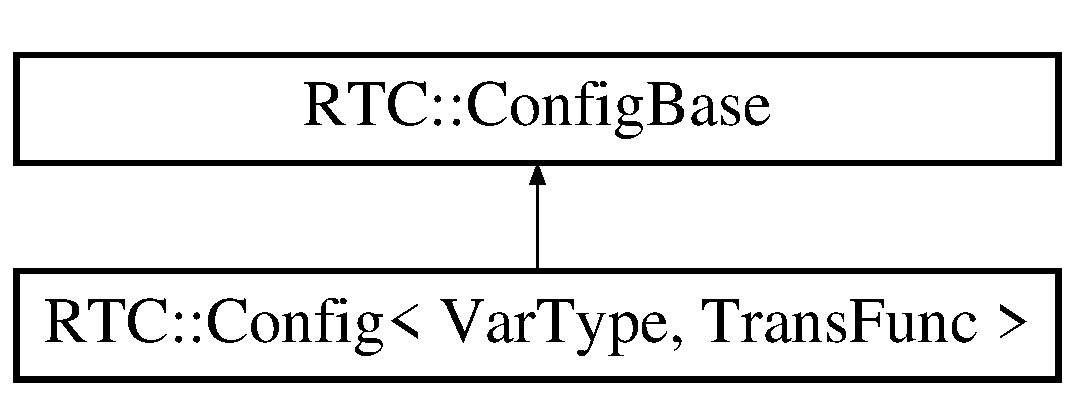
\includegraphics[height=2cm]{structRTC_1_1ConfigBase}
\end{center}
\end{figure}
\subsection*{Public Member Functions}
\begin{DoxyCompactItemize}
\item 
{\bf ConfigBase} (const char $\ast$name\_\-, const char $\ast$def\_\-val)
\begin{DoxyCompactList}\small\item\em Constructer. \item\end{DoxyCompactList}\item 
virtual {\bf $\sim$ConfigBase} (void)
\begin{DoxyCompactList}\small\item\em Virtual Destructor. \item\end{DoxyCompactList}\item 
virtual bool {\bf update} (const char $\ast$val)=0
\begin{DoxyCompactList}\small\item\em Pure virtual function to update configuration parameter values. \item\end{DoxyCompactList}\end{DoxyCompactItemize}
\subsection*{Public Attributes}
\begin{DoxyCompactItemize}
\item 
const char $\ast$ {\bf name}
\begin{DoxyCompactList}\small\item\em Configuration name. \item\end{DoxyCompactList}\item 
const char $\ast$ {\bf default\_\-value}
\begin{DoxyCompactList}\small\item\em Default value in string format. \item\end{DoxyCompactList}\end{DoxyCompactItemize}


\subsection{Detailed Description}
\doxyref{ConfigBase}{p.}{structRTC_1_1ConfigBase} abstract class. This is the abstract interface class to hold various configuration information. Concrete configuration classes must implement the following pure virtual functions.

This class provides public interface as follows.
\begin{DoxyItemize}
\item \doxyref{update()}{p.}{structRTC_1_1ConfigBase_a353307f47fe534865db2a9173380e38c}: update configuration parameter value
\end{DoxyItemize}

\begin{DoxySince}{Since}
0.4.0 
\end{DoxySince}


\subsection{Constructor \& Destructor Documentation}
\index{RTC::ConfigBase@{RTC::ConfigBase}!ConfigBase@{ConfigBase}}
\index{ConfigBase@{ConfigBase}!RTC::ConfigBase@{RTC::ConfigBase}}
\subsubsection[{ConfigBase}]{\setlength{\rightskip}{0pt plus 5cm}RTC::ConfigBase::ConfigBase (const char $\ast$ {\em name\_\-}, \/  const char $\ast$ {\em def\_\-val})\hspace{0.3cm}{\ttfamily  [inline]}}\label{structRTC_1_1ConfigBase_a3bc7089cfd7b148209890abb2cb2b9cd}


Constructer. 

Constructer


\begin{DoxyParams}{Parameters}
\item[{\em name\_\-}]Configuration name \item[{\em def\_\-val}]Default value in string format \end{DoxyParams}
\index{RTC::ConfigBase@{RTC::ConfigBase}!$\sim$ConfigBase@{$\sim$ConfigBase}}
\index{$\sim$ConfigBase@{$\sim$ConfigBase}!RTC::ConfigBase@{RTC::ConfigBase}}
\subsubsection[{$\sim$ConfigBase}]{\setlength{\rightskip}{0pt plus 5cm}virtual RTC::ConfigBase::$\sim$ConfigBase (void)\hspace{0.3cm}{\ttfamily  [inline, virtual]}}\label{structRTC_1_1ConfigBase_a305aec103d2c6693f632cc0c8ca3ceba}


Virtual Destructor. 

Virtual Destructor 

\subsection{Member Function Documentation}
\index{RTC::ConfigBase@{RTC::ConfigBase}!update@{update}}
\index{update@{update}!RTC::ConfigBase@{RTC::ConfigBase}}
\subsubsection[{update}]{\setlength{\rightskip}{0pt plus 5cm}virtual bool RTC::ConfigBase::update (const char $\ast$ {\em val})\hspace{0.3cm}{\ttfamily  [pure virtual]}}\label{structRTC_1_1ConfigBase_a353307f47fe534865db2a9173380e38c}


Pure virtual function to update configuration parameter values. 

Pure virtual function to update configuration parameter by the configuration value.


\begin{DoxyParams}{Parameters}
\item[{\em val}]The parameter values converted into character string format\end{DoxyParams}
\begin{DoxyReturn}{Returns}
Result of the setup 
\end{DoxyReturn}


Implemented in {\bf RTC::Config$<$ VarType, TransFunc $>$} \doxyref{}{p.}{classRTC_1_1Config_ae62b81ad2d80a5f40f594f473f9556fa}.



\subsection{Member Data Documentation}
\index{RTC::ConfigBase@{RTC::ConfigBase}!default\_\-value@{default\_\-value}}
\index{default\_\-value@{default\_\-value}!RTC::ConfigBase@{RTC::ConfigBase}}
\subsubsection[{default\_\-value}]{\setlength{\rightskip}{0pt plus 5cm}const char$\ast$ {\bf RTC::ConfigBase::default\_\-value}}\label{structRTC_1_1ConfigBase_a160ecb767e940bfd30f46d95032588d1}


Default value in string format. 

\index{RTC::ConfigBase@{RTC::ConfigBase}!name@{name}}
\index{name@{name}!RTC::ConfigBase@{RTC::ConfigBase}}
\subsubsection[{name}]{\setlength{\rightskip}{0pt plus 5cm}const char$\ast$ {\bf RTC::ConfigBase::name}}\label{structRTC_1_1ConfigBase_a110474d849e54c4b91625763d04a2335}


Configuration name. 


\section{SDOPackage::Configuration\_\-impl Class Reference}
\label{classSDOPackage_1_1Configuration__impl}\index{SDOPackage::Configuration\_\-impl@{SDOPackage::Configuration\_\-impl}}


Configuration implementation class.  




{\ttfamily \#include $<$SdoConfiguration.h$>$}

\subsection*{Classes}
\begin{DoxyCompactItemize}
\item 
struct {\bf config\_\-id}
\begin{DoxyCompactList}\small\item\em Functor for ConfigurationSet. \item\end{DoxyCompactList}\item 
struct {\bf nv\_\-name}
\begin{DoxyCompactList}\small\item\em Functor for NVList. \item\end{DoxyCompactList}\item 
struct {\bf org\_\-id}
\begin{DoxyCompactList}\small\item\em Functor for Organization. \item\end{DoxyCompactList}\end{DoxyCompactItemize}
\subsection*{Public Member Functions}
\begin{DoxyCompactItemize}
\item 
{\bf Configuration\_\-impl} ({\bf RTC::ConfigAdmin} \&configAdmin, {\bf RTC::SdoServiceAdmin} \&sdoServiceAdmin)
\begin{DoxyCompactList}\small\item\em Constructor. \item\end{DoxyCompactList}\item 
virtual {\bf $\sim$Configuration\_\-impl} (void)
\item 
virtual CORBA::Boolean {\bf set\_\-device\_\-profile} (const DeviceProfile \&dProfile)  throw (CORBA::SystemException,	     InvalidParameter, NotAvailable, InternalError)
\begin{DoxyCompactList}\small\item\em [CORBA interface] Set DeviceProfile of \doxyref{SDO}{p.}{classSDO} \item\end{DoxyCompactList}\item 
virtual CORBA::Boolean {\bf add\_\-service\_\-profile} (const ServiceProfile \&sProfile)  throw (CORBA::SystemException,	     InvalidParameter, NotAvailable, InternalError)
\begin{DoxyCompactList}\small\item\em [CORBA interface] Set SDO's ServiceProfile \item\end{DoxyCompactList}\item 
virtual CORBA::Boolean {\bf add\_\-organization} (Organization\_\-ptr org)  throw (CORBA::SystemException,	     InvalidParameter, NotAvailable, InternalError)
\begin{DoxyCompactList}\small\item\em [CORBA interface] Add Organization \item\end{DoxyCompactList}\item 
virtual CORBA::Boolean {\bf remove\_\-service\_\-profile} (const char $\ast$id)  throw (CORBA::SystemException,	     InvalidParameter, NotAvailable, InternalError)
\begin{DoxyCompactList}\small\item\em [CORBA interface] Remove ServiceProfile \item\end{DoxyCompactList}\item 
virtual CORBA::Boolean {\bf remove\_\-organization} (const char $\ast$organization\_\-id)  throw (CORBA::SystemException,	     InvalidParameter, NotAvailable, InternalError)
\begin{DoxyCompactList}\small\item\em [CORBA interface] Remove the reference of Organization \item\end{DoxyCompactList}\item 
virtual ParameterList $\ast$ {\bf get\_\-configuration\_\-parameters} ()  throw (CORBA::SystemException,	     NotAvailable, InternalError)
\begin{DoxyCompactList}\small\item\em [CORBA interface] Get a list of configuration parameters \item\end{DoxyCompactList}\item 
virtual NVList $\ast$ {\bf get\_\-configuration\_\-parameter\_\-values} ()  throw (CORBA::SystemException,	     NotAvailable, InternalError)
\begin{DoxyCompactList}\small\item\em [CORBA interface] Get a list of the value of configuration parameters \item\end{DoxyCompactList}\item 
virtual CORBA::Any $\ast$ {\bf get\_\-configuration\_\-parameter\_\-value} (const char $\ast$name)  throw (CORBA::SystemException,	     InvalidParameter, NotAvailable, InternalError)
\begin{DoxyCompactList}\small\item\em [CORBA interface] Get the value of configuration parameter \item\end{DoxyCompactList}\item 
virtual CORBA::Boolean {\bf set\_\-configuration\_\-parameter} (const char $\ast$name, const CORBA::Any \&value)  throw (CORBA::SystemException,	     InvalidParameter, NotAvailable, InternalError)
\begin{DoxyCompactList}\small\item\em [CORBA interface] Modify the configuration parameter value \item\end{DoxyCompactList}\item 
virtual ConfigurationSetList $\ast$ {\bf get\_\-configuration\_\-sets} ()  throw (CORBA::SystemException,	     NotAvailable, InternalError)
\begin{DoxyCompactList}\small\item\em [CORBA interface] Get a list of ConfigurationSet \item\end{DoxyCompactList}\item 
virtual ConfigurationSet $\ast$ {\bf get\_\-configuration\_\-set} (const char $\ast${\bf config\_\-id})  throw (CORBA::SystemException,	     NotAvailable, InternalError)
\begin{DoxyCompactList}\small\item\em [CORBA interface] Get a ConfigurationSet \item\end{DoxyCompactList}\item 
virtual ConfigurationSet $\ast$ {\bf get\_\-active\_\-configuration\_\-set} ()  throw (CORBA::SystemException,	     NotAvailable, InternalError)
\begin{DoxyCompactList}\small\item\em [CORBA interface] Get active ConfigurationSet \item\end{DoxyCompactList}\item 
virtual CORBA::Boolean {\bf add\_\-configuration\_\-set} (const ConfigurationSet \&configuration\_\-set)  throw (CORBA::SystemException,	     InvalidParameter, NotAvailable, InternalError)
\begin{DoxyCompactList}\small\item\em [CORBA interface] Add ConfigurationSet \item\end{DoxyCompactList}\item 
virtual CORBA::Boolean {\bf set\_\-configuration\_\-set\_\-values} (const ConfigurationSet \&configuration\_\-set)  throw (CORBA::SystemException,	     InvalidParameter, NotAvailable, InternalError)
\begin{DoxyCompactList}\small\item\em [CORBA interface] Set ConfigurationSet \item\end{DoxyCompactList}\item 
virtual CORBA::Boolean {\bf remove\_\-configuration\_\-set} (const char $\ast${\bf config\_\-id})  throw (CORBA::SystemException,	     InvalidParameter, NotAvailable, InternalError)
\begin{DoxyCompactList}\small\item\em [CORBA interface] Remove ConfigurationSet \item\end{DoxyCompactList}\item 
virtual CORBA::Boolean {\bf activate\_\-configuration\_\-set} (const char $\ast${\bf config\_\-id})  throw (CORBA::SystemException,	     InvalidParameter, NotAvailable, InternalError)
\begin{DoxyCompactList}\small\item\em [CORBA interface] Activate ConfigurationSet \item\end{DoxyCompactList}\item 
Configuration\_\-ptr {\bf getObjRef} ()
\begin{DoxyCompactList}\small\item\em Get object reference. \item\end{DoxyCompactList}\item 
const DeviceProfile {\bf getDeviceProfile} ()
\begin{DoxyCompactList}\small\item\em Get the DeviceProfile of \doxyref{SDO}{p.}{classSDO}. \item\end{DoxyCompactList}\item 
const OrganizationList {\bf getOrganizations} ()
\begin{DoxyCompactList}\small\item\em Get a list of Organization of \doxyref{SDO}{p.}{classSDO}. \item\end{DoxyCompactList}\end{DoxyCompactItemize}
\subsection*{Protected Member Functions}
\begin{DoxyCompactItemize}
\item 
const std::string {\bf getUUID} () const 
\begin{DoxyCompactList}\small\item\em Generate UUID. \item\end{DoxyCompactList}\end{DoxyCompactItemize}
\subsection*{Protected Attributes}
\begin{DoxyCompactItemize}
\item 
::{\bf RTC::Logger} {\bf rtclog}
\item 
Configuration\_\-var {\bf m\_\-objref}
\begin{DoxyCompactList}\small\item\em The reference to CORBA object. \item\end{DoxyCompactList}\item 
DeviceProfile {\bf m\_\-deviceProfile}
\begin{DoxyCompactList}\small\item\em \doxyref{SDO}{p.}{classSDO} DeviceProfile with mutex lock. \item\end{DoxyCompactList}\item 
{\bf Mutex} {\bf m\_\-dprofile\_\-mutex}
\item 
ParameterList {\bf m\_\-parameters}
\begin{DoxyCompactList}\small\item\em \doxyref{SDO}{p.}{classSDO} Parameter. \item\end{DoxyCompactList}\item 
{\bf Mutex} {\bf m\_\-params\_\-mutex}
\item 
{\bf RTC::ConfigAdmin} \& {\bf m\_\-configsets}
\begin{DoxyCompactList}\small\item\em \doxyref{SDO}{p.}{classSDO} ConfigurationSetList with mutex lock. \item\end{DoxyCompactList}\item 
{\bf Mutex} {\bf m\_\-config\_\-mutex}
\item 
{\bf RTC::SdoServiceAdmin} \& {\bf m\_\-sdoservice}
\begin{DoxyCompactList}\small\item\em \doxyref{SDO}{p.}{classSDO} Service admin object with mutex lock. \item\end{DoxyCompactList}\item 
{\bf Mutex} {\bf m\_\-sdoservice\_\-mutex}
\item 
OrganizationList {\bf m\_\-organizations}
\begin{DoxyCompactList}\small\item\em \doxyref{SDO}{p.}{classSDO} OrganizationList with mutex lock. \item\end{DoxyCompactList}\item 
{\bf Mutex} {\bf m\_\-org\_\-mutex}
\end{DoxyCompactItemize}


\subsection{Detailed Description}
Configuration implementation class. Configuration interface provides operations to add or remove data specified in resource data model. These operations provide functions to change DeviceProfile, ServiceProfile, ConfigurationProfile, and Organization. This \doxyref{SDO}{p.}{classSDO} specification does not address access control or security aspects.

Different configurations can be stored for simple and quick activation. Different predefined configurations are stored as different ConfigurationSets or configuration profile. A ConfigurationSet stores the value of all properties assigned for the particular configuration along with its unique id and description to identify and describe the configuration respectively. Operations in the configuration interface help manage these ConfigurationSets.


\begin{DoxyItemize}
\item ConfigurationSet: id, description, one configuration set to consist of NVList
\item ConfigurationSetList: List of ConfigurationSet
\item Parameter: Parameter definition consist of name, type and allowed\_\-values
\item ActiveConfigurationSet: One set of configuration set that is valid.
\end{DoxyItemize}

The following functions do processing to ParameterList.
\begin{DoxyItemize}
\item \doxyref{get\_\-configuration\_\-parameters()}{p.}{classSDOPackage_1_1Configuration__impl_a719cf33d63573f2c77e76cc0bd7c95a1}
\end{DoxyItemize}

The following functions do processing to active ConfigurationSet
\begin{DoxyItemize}
\item \doxyref{get\_\-configuration\_\-parameter\_\-values()}{p.}{classSDOPackage_1_1Configuration__impl_a35e8b8d9af4a2b4f78e0a86244bff558}
\item \doxyref{get\_\-configuration\_\-parameter\_\-value()}{p.}{classSDOPackage_1_1Configuration__impl_a27497be83bfe0bacde9fc4f89c861077}
\item \doxyref{set\_\-configuration\_\-parameter()}{p.}{classSDOPackage_1_1Configuration__impl_ad8be3428eca25a151d9e0a11447828b0}
\end{DoxyItemize}

The following functions do processing to ConfigurationSetList
\begin{DoxyItemize}
\item \doxyref{get\_\-configuration\_\-sets()}{p.}{classSDOPackage_1_1Configuration__impl_a77844f4a7407bc48c11a455f89d32f4d}
\item \doxyref{get\_\-configuration\_\-set()}{p.}{classSDOPackage_1_1Configuration__impl_a9053da972df19c6411b0326eb5239b39}
\item \doxyref{set\_\-configuration\_\-set\_\-values()}{p.}{classSDOPackage_1_1Configuration__impl_a89a53c51f56795a098f3be79052413ad}
\item \doxyref{get\_\-active\_\-configuration\_\-set()}{p.}{classSDOPackage_1_1Configuration__impl_aee57768379674404422130e0f04468e2}
\item \doxyref{add\_\-configuration\_\-set()}{p.}{classSDOPackage_1_1Configuration__impl_a3765b45decf597811c3e0f562b914fab}
\item \doxyref{remove\_\-configuration\_\-set()}{p.}{classSDOPackage_1_1Configuration__impl_ac82aad180dcb37a3d652abb0e368da0a}
\item \doxyref{activate\_\-configuration\_\-set()}{p.}{classSDOPackage_1_1Configuration__impl_a7264893ed1b678fcf301a73304bf77b7}
\end{DoxyItemize}

\begin{DoxySince}{Since}
0.4.0 
\end{DoxySince}


\subsection{Constructor \& Destructor Documentation}
\index{SDOPackage::Configuration\_\-impl@{SDOPackage::Configuration\_\-impl}!Configuration\_\-impl@{Configuration\_\-impl}}
\index{Configuration\_\-impl@{Configuration\_\-impl}!SDOPackage::Configuration_impl@{SDOPackage::Configuration\_\-impl}}
\subsubsection[{Configuration\_\-impl}]{\setlength{\rightskip}{0pt plus 5cm}SDOPackage::Configuration\_\-impl::Configuration\_\-impl ({\bf RTC::ConfigAdmin} \& {\em configAdmin}, \/  {\bf RTC::SdoServiceAdmin} \& {\em sdoServiceAdmin})}\label{classSDOPackage_1_1Configuration__impl_aa9a10c1aa6abb899a866f501ba2c4075}


Constructor. 

Constructor


\begin{DoxyParams}{Parameters}
\item[{\em configAdmin}]ConfigurationSetList \end{DoxyParams}
\index{SDOPackage::Configuration\_\-impl@{SDOPackage::Configuration\_\-impl}!$\sim$Configuration\_\-impl@{$\sim$Configuration\_\-impl}}
\index{$\sim$Configuration\_\-impl@{$\sim$Configuration\_\-impl}!SDOPackage::Configuration_impl@{SDOPackage::Configuration\_\-impl}}
\subsubsection[{$\sim$Configuration\_\-impl}]{\setlength{\rightskip}{0pt plus 5cm}virtual SDOPackage::Configuration\_\-impl::$\sim$Configuration\_\-impl (void)\hspace{0.3cm}{\ttfamily  [virtual]}}\label{classSDOPackage_1_1Configuration__impl_a64d2363427a77cb4b8e79e2f6d55e6d7}
Virtual destractor. 

\subsection{Member Function Documentation}
\index{SDOPackage::Configuration\_\-impl@{SDOPackage::Configuration\_\-impl}!activate\_\-configuration\_\-set@{activate\_\-configuration\_\-set}}
\index{activate\_\-configuration\_\-set@{activate\_\-configuration\_\-set}!SDOPackage::Configuration_impl@{SDOPackage::Configuration\_\-impl}}
\subsubsection[{activate\_\-configuration\_\-set}]{\setlength{\rightskip}{0pt plus 5cm}virtual CORBA::Boolean SDOPackage::Configuration\_\-impl::activate\_\-configuration\_\-set (const char $\ast$ {\em config\_\-id})  throw (CORBA::SystemException,	     InvalidParameter, NotAvailable, InternalError)\hspace{0.3cm}{\ttfamily  [virtual]}}\label{classSDOPackage_1_1Configuration__impl_a7264893ed1b678fcf301a73304bf77b7}


[CORBA interface] Activate ConfigurationSet 

This operation activates one of the stored ConfigurationSets in the ConfigurationProfile. This operation activates the specified stored ConfigurationSets. This means that the configuration properties of the \doxyref{SDO}{p.}{classSDO} are changed as the values of these properties specified in the stored ConfigurationSet. In other words, values of the specified ConfigurationSet are now copied to the active configuration.


\begin{DoxyParams}{Parameters}
\item[{\em \doxyref{config\_\-id}{p.}{structSDOPackage_1_1Configuration__impl_1_1config__id}}]Identifier of ConfigurationSet to be activated.\end{DoxyParams}
\begin{DoxyReturn}{Returns}
If the operation was successfully completed.
\end{DoxyReturn}

\begin{DoxyExceptions}{Exceptions}
\item[{\em SDONotExists}]The target \doxyref{SDO}{p.}{classSDO} does not exist.(This exception is mapped to CORBA standard system exception OBJECT\_\-NOT\_\-EXIST.) \item[{\em InvalidParameter}]The argument (\char`\"{}configID\char`\"{}) is null or there is no configuration set with identifier specified by the argument. \item[{\em NotAvailable}]The target \doxyref{SDO}{p.}{classSDO} is reachable but cannot respond. \item[{\em InternalError}]The target \doxyref{SDO}{p.}{classSDO} cannot execute the operation completely due to some internal error. \end{DoxyExceptions}
\index{SDOPackage::Configuration\_\-impl@{SDOPackage::Configuration\_\-impl}!add\_\-configuration\_\-set@{add\_\-configuration\_\-set}}
\index{add\_\-configuration\_\-set@{add\_\-configuration\_\-set}!SDOPackage::Configuration_impl@{SDOPackage::Configuration\_\-impl}}
\subsubsection[{add\_\-configuration\_\-set}]{\setlength{\rightskip}{0pt plus 5cm}virtual CORBA::Boolean SDOPackage::Configuration\_\-impl::add\_\-configuration\_\-set (const ConfigurationSet \& {\em configuration\_\-set})  throw (CORBA::SystemException,	     InvalidParameter, NotAvailable, InternalError)\hspace{0.3cm}{\ttfamily  [virtual]}}\label{classSDOPackage_1_1Configuration__impl_a3765b45decf597811c3e0f562b914fab}


[CORBA interface] Add ConfigurationSet 

This operation adds a ConfigurationSet to the ConfigurationProfile.


\begin{DoxyParams}{Parameters}
\item[{\em configuration\_\-set}]The ConfigurationSet that is added.\end{DoxyParams}
\begin{DoxyReturn}{Returns}
If the operation was successfully completed.
\end{DoxyReturn}

\begin{DoxyExceptions}{Exceptions}
\item[{\em SDONotExists}]The target \doxyref{SDO}{p.}{classSDO} does not exist.(This exception is mapped to CORBA standard system exception OBJECT\_\-NOT\_\-EXIST.) \item[{\em InvalidParameter}]The argument \char`\"{}configurationSet\char`\"{} is null, or one of the attributes defining \char`\"{}configurationSet\char`\"{} is invalid, or the specified identifier of the configuration set already exists. \item[{\em NotAvailable}]The target \doxyref{SDO}{p.}{classSDO} is reachable but cannot respond. \item[{\em InternalError}]The target \doxyref{SDO}{p.}{classSDO} cannot execute the operation completely due to some internal error. \end{DoxyExceptions}
\index{SDOPackage::Configuration\_\-impl@{SDOPackage::Configuration\_\-impl}!add\_\-organization@{add\_\-organization}}
\index{add\_\-organization@{add\_\-organization}!SDOPackage::Configuration_impl@{SDOPackage::Configuration\_\-impl}}
\subsubsection[{add\_\-organization}]{\setlength{\rightskip}{0pt plus 5cm}virtual CORBA::Boolean SDOPackage::Configuration\_\-impl::add\_\-organization (Organization\_\-ptr {\em org})  throw (CORBA::SystemException,	     InvalidParameter, NotAvailable, InternalError)\hspace{0.3cm}{\ttfamily  [virtual]}}\label{classSDOPackage_1_1Configuration__impl_a7963b66fe9bdbac8b23528ec5c7bca79}


[CORBA interface] Add Organization 

This operation adds reference of an Organization object.


\begin{DoxyParams}{Parameters}
\item[{\em org}]Organization to be added.\end{DoxyParams}
\begin{DoxyReturn}{Returns}
If the operation was successfully completed.
\end{DoxyReturn}

\begin{DoxyExceptions}{Exceptions}
\item[{\em SDONotExists}]The target \doxyref{SDO}{p.}{classSDO} does not exist.(This exception is mapped to CORBA standard system exception OBJECT\_\-NOT\_\-EXIST.) \item[{\em NotAvailable}]The target \doxyref{SDO}{p.}{classSDO} is reachable but cannot respond. \item[{\em InvalidParameter}]The argument “organization” is null. \item[{\em InternalError}]The target \doxyref{SDO}{p.}{classSDO} cannot execute the operation completely due to some internal error. \end{DoxyExceptions}
\index{SDOPackage::Configuration\_\-impl@{SDOPackage::Configuration\_\-impl}!add\_\-service\_\-profile@{add\_\-service\_\-profile}}
\index{add\_\-service\_\-profile@{add\_\-service\_\-profile}!SDOPackage::Configuration_impl@{SDOPackage::Configuration\_\-impl}}
\subsubsection[{add\_\-service\_\-profile}]{\setlength{\rightskip}{0pt plus 5cm}virtual CORBA::Boolean SDOPackage::Configuration\_\-impl::add\_\-service\_\-profile (const ServiceProfile \& {\em sProfile})  throw (CORBA::SystemException,	     InvalidParameter, NotAvailable, InternalError)\hspace{0.3cm}{\ttfamily  [virtual]}}\label{classSDOPackage_1_1Configuration__impl_a42e08f0ca92fa64b4728c499d1e4e707}


[CORBA interface] Set SDO's ServiceProfile 

This operation adds ServiceProfile to the target \doxyref{SDO}{p.}{classSDO} that navigates this Configuration interface. If the id in argument ServiceProfile is null, new id is created and the ServiceProfile is stored. If the id is not null, the target \doxyref{SDO}{p.}{classSDO} searches for ServiceProfile in it with the same id. It adds the ServiceProfile if not exist, or overwrites if exist.


\begin{DoxyParams}{Parameters}
\item[{\em sProfile}]ServiceProfile to be added.\end{DoxyParams}
\begin{DoxyReturn}{Returns}
If the operation was successfully completed.
\end{DoxyReturn}

\begin{DoxyExceptions}{Exceptions}
\item[{\em SDONotExists}]The target \doxyref{SDO}{p.}{classSDO} does not exist.(This exception is mapped to CORBA standard system exception OBJECT\_\-NOT\_\-EXIST.) \item[{\em NotAvailable}]The target \doxyref{SDO}{p.}{classSDO} is reachable but cannot respond. \item[{\em InvalidParameter}]The argument \char`\"{}sProfile\char`\"{} is null. \item[{\em InternalError}]The target \doxyref{SDO}{p.}{classSDO} cannot execute the operation completely due to some internal error. \end{DoxyExceptions}
\index{SDOPackage::Configuration\_\-impl@{SDOPackage::Configuration\_\-impl}!get\_\-active\_\-configuration\_\-set@{get\_\-active\_\-configuration\_\-set}}
\index{get\_\-active\_\-configuration\_\-set@{get\_\-active\_\-configuration\_\-set}!SDOPackage::Configuration_impl@{SDOPackage::Configuration\_\-impl}}
\subsubsection[{get\_\-active\_\-configuration\_\-set}]{\setlength{\rightskip}{0pt plus 5cm}virtual ConfigurationSet$\ast$ SDOPackage::Configuration\_\-impl::get\_\-active\_\-configuration\_\-set ()  throw (CORBA::SystemException,	     NotAvailable, InternalError)\hspace{0.3cm}{\ttfamily  [virtual]}}\label{classSDOPackage_1_1Configuration__impl_aee57768379674404422130e0f04468e2}


[CORBA interface] Get active ConfigurationSet 

This operation returns the current active ConfigurationSet of an \doxyref{SDO}{p.}{classSDO} (i.e., if the current configuration of the \doxyref{SDO}{p.}{classSDO} was set using predefined configuration set). ConfigurationSet cannot be considered active if the:


\begin{DoxyItemize}
\item Current configuration of the \doxyref{SDO}{p.}{classSDO} was not set using any predefined ConfigurationSet, or
\item Configuration of the \doxyref{SDO}{p.}{classSDO} was changed after it has been active, or
\item ConfigurationSet that was used to configure the \doxyref{SDO}{p.}{classSDO} was modified.
\end{DoxyItemize}

Empty ConfigurationSet is returned in these cases.

\begin{DoxyReturn}{Returns}
The active ConfigurationSet.
\end{DoxyReturn}

\begin{DoxyExceptions}{Exceptions}
\item[{\em SDONotExists}]The target \doxyref{SDO}{p.}{classSDO} does not exist.(This exception is mapped to CORBA standard system exception OBJECT\_\-NOT\_\-EXIST.) \item[{\em NotAvailable}]The target \doxyref{SDO}{p.}{classSDO} is reachable but cannot respond. \item[{\em InternalError}]The target \doxyref{SDO}{p.}{classSDO} cannot execute the operation completely due to some internal error. \end{DoxyExceptions}
\index{SDOPackage::Configuration\_\-impl@{SDOPackage::Configuration\_\-impl}!get\_\-configuration\_\-parameter\_\-value@{get\_\-configuration\_\-parameter\_\-value}}
\index{get\_\-configuration\_\-parameter\_\-value@{get\_\-configuration\_\-parameter\_\-value}!SDOPackage::Configuration_impl@{SDOPackage::Configuration\_\-impl}}
\subsubsection[{get\_\-configuration\_\-parameter\_\-value}]{\setlength{\rightskip}{0pt plus 5cm}virtual CORBA::Any$\ast$ SDOPackage::Configuration\_\-impl::get\_\-configuration\_\-parameter\_\-value (const char $\ast$ {\em name})  throw (CORBA::SystemException,	     InvalidParameter, NotAvailable, InternalError)\hspace{0.3cm}{\ttfamily  [virtual]}}\label{classSDOPackage_1_1Configuration__impl_a27497be83bfe0bacde9fc4f89c861077}


[CORBA interface] Get the value of configuration parameter 

This operation returns a value of parameter that is specified by argument \char`\"{}name.\char`\"{}


\begin{DoxyParams}{Parameters}
\item[{\em name}]Name of the parameter whose value is requested.\end{DoxyParams}
\begin{DoxyReturn}{Returns}
The value of the specified parameter.
\end{DoxyReturn}

\begin{DoxyExceptions}{Exceptions}
\item[{\em SDONotExists}]The target \doxyref{SDO}{p.}{classSDO} does not exist.(This exception is mapped to CORBA standard system exception OBJECT\_\-NOT\_\-EXIST.) \item[{\em InvalidParameter}]The value of the argument \char`\"{}name\char`\"{} is empty String, or null, or the parameter that is specified by argument \char`\"{}name\char`\"{} does not exist. \item[{\em NotAvailable}]The target \doxyref{SDO}{p.}{classSDO} is reachable but cannot respond. \item[{\em InternalError}]The target \doxyref{SDO}{p.}{classSDO} cannot execute the operation completely due to some internal error. \end{DoxyExceptions}
\index{SDOPackage::Configuration\_\-impl@{SDOPackage::Configuration\_\-impl}!get\_\-configuration\_\-parameter\_\-values@{get\_\-configuration\_\-parameter\_\-values}}
\index{get\_\-configuration\_\-parameter\_\-values@{get\_\-configuration\_\-parameter\_\-values}!SDOPackage::Configuration_impl@{SDOPackage::Configuration\_\-impl}}
\subsubsection[{get\_\-configuration\_\-parameter\_\-values}]{\setlength{\rightskip}{0pt plus 5cm}virtual NVList$\ast$ SDOPackage::Configuration\_\-impl::get\_\-configuration\_\-parameter\_\-values ()  throw (CORBA::SystemException,	     NotAvailable, InternalError)\hspace{0.3cm}{\ttfamily  [virtual]}}\label{classSDOPackage_1_1Configuration__impl_a35e8b8d9af4a2b4f78e0a86244bff558}


[CORBA interface] Get a list of the value of configuration parameters 

This operation returns all configuration parameters and their values.

\begin{DoxyReturn}{Returns}
List of all configuration parameters and their values.
\end{DoxyReturn}

\begin{DoxyExceptions}{Exceptions}
\item[{\em SDONotExists}]The target \doxyref{SDO}{p.}{classSDO} does not exist.(This exception is mapped to CORBA standard system exception OBJECT\_\-NOT\_\-EXIST.) \item[{\em NotAvailable}]The target \doxyref{SDO}{p.}{classSDO} is reachable but cannot respond. \item[{\em InternalError}]The target \doxyref{SDO}{p.}{classSDO} cannot execute the operation completely due to some internal error. \end{DoxyExceptions}
\index{SDOPackage::Configuration\_\-impl@{SDOPackage::Configuration\_\-impl}!get\_\-configuration\_\-parameters@{get\_\-configuration\_\-parameters}}
\index{get\_\-configuration\_\-parameters@{get\_\-configuration\_\-parameters}!SDOPackage::Configuration_impl@{SDOPackage::Configuration\_\-impl}}
\subsubsection[{get\_\-configuration\_\-parameters}]{\setlength{\rightskip}{0pt plus 5cm}virtual ParameterList$\ast$ SDOPackage::Configuration\_\-impl::get\_\-configuration\_\-parameters ()  throw (CORBA::SystemException,	     NotAvailable, InternalError)\hspace{0.3cm}{\ttfamily  [virtual]}}\label{classSDOPackage_1_1Configuration__impl_a719cf33d63573f2c77e76cc0bd7c95a1}


[CORBA interface] Get a list of configuration parameters 

This operation returns a list of Parameters. An empty list is returned if the \doxyref{SDO}{p.}{classSDO} does not have any configurable parameter.

\begin{DoxyReturn}{Returns}
The list with definitions of parameters characterizing the configuration.
\end{DoxyReturn}

\begin{DoxyExceptions}{Exceptions}
\item[{\em SDONotExists}]The target \doxyref{SDO}{p.}{classSDO} does not exist.(This exception is mapped to CORBA standard system exception OBJECT\_\-NOT\_\-EXIST.) \item[{\em NotAvailable}]The target \doxyref{SDO}{p.}{classSDO} is reachable but cannot respond. \item[{\em InternalError}]The target \doxyref{SDO}{p.}{classSDO} cannot execute the operation completely due to some internal error. \end{DoxyExceptions}
\index{SDOPackage::Configuration\_\-impl@{SDOPackage::Configuration\_\-impl}!get\_\-configuration\_\-set@{get\_\-configuration\_\-set}}
\index{get\_\-configuration\_\-set@{get\_\-configuration\_\-set}!SDOPackage::Configuration_impl@{SDOPackage::Configuration\_\-impl}}
\subsubsection[{get\_\-configuration\_\-set}]{\setlength{\rightskip}{0pt plus 5cm}virtual ConfigurationSet$\ast$ SDOPackage::Configuration\_\-impl::get\_\-configuration\_\-set (const char $\ast$ {\em config\_\-id})  throw (CORBA::SystemException,	     NotAvailable, InternalError)\hspace{0.3cm}{\ttfamily  [virtual]}}\label{classSDOPackage_1_1Configuration__impl_a9053da972df19c6411b0326eb5239b39}


[CORBA interface] Get a ConfigurationSet 

This operation returns the ConfigurationSet specified by the parameter configurationSetID.


\begin{DoxyParams}{Parameters}
\item[{\em \doxyref{config\_\-id}{p.}{structSDOPackage_1_1Configuration__impl_1_1config__id}}]Identifier of ConfigurationSet requested.\end{DoxyParams}
\begin{DoxyReturn}{Returns}
The configuration set specified by the parameter \doxyref{config\_\-id}{p.}{structSDOPackage_1_1Configuration__impl_1_1config__id}.
\end{DoxyReturn}

\begin{DoxyExceptions}{Exceptions}
\item[{\em SDONotExists}]The target \doxyref{SDO}{p.}{classSDO} does not exist.(This exception is mapped to CORBA standard system exception OBJECT\_\-NOT\_\-EXIST.) \item[{\em InvalidParameter}]The parameter 'config\_\-id' is null or there are no ConfigurationSets stored with such id. \item[{\em NotAvailable}]The target \doxyref{SDO}{p.}{classSDO} is reachable but cannot respond. \item[{\em InternalError}]The target \doxyref{SDO}{p.}{classSDO} cannot execute the operation completely due to some internal error. \end{DoxyExceptions}
\index{SDOPackage::Configuration\_\-impl@{SDOPackage::Configuration\_\-impl}!get\_\-configuration\_\-sets@{get\_\-configuration\_\-sets}}
\index{get\_\-configuration\_\-sets@{get\_\-configuration\_\-sets}!SDOPackage::Configuration_impl@{SDOPackage::Configuration\_\-impl}}
\subsubsection[{get\_\-configuration\_\-sets}]{\setlength{\rightskip}{0pt plus 5cm}virtual ConfigurationSetList$\ast$ SDOPackage::Configuration\_\-impl::get\_\-configuration\_\-sets ()  throw (CORBA::SystemException,	     NotAvailable, InternalError)\hspace{0.3cm}{\ttfamily  [virtual]}}\label{classSDOPackage_1_1Configuration__impl_a77844f4a7407bc48c11a455f89d32f4d}


[CORBA interface] Get a list of ConfigurationSet 

This operation returns a list of ConfigurationSets that the ConfigurationProfile has. An empty list is returned if the \doxyref{SDO}{p.}{classSDO} does not have any ConfigurationSets. This operation returns a list of all ConfigurationSets of the \doxyref{SDO}{p.}{classSDO}. If no predefined ConfigurationSets exist, then empty list is returned.

\begin{DoxyReturn}{Returns}
The list of stored configuration with their current values.
\end{DoxyReturn}

\begin{DoxyExceptions}{Exceptions}
\item[{\em SDONotExists}]The target \doxyref{SDO}{p.}{classSDO} does not exist.(This exception is mapped to CORBA standard system exception OBJECT\_\-NOT\_\-EXIST.) \item[{\em NotAvailable}]The target \doxyref{SDO}{p.}{classSDO} is reachable but cannot respond. \item[{\em InternalError}]The target \doxyref{SDO}{p.}{classSDO} cannot execute the operation completely due to some internal error. \end{DoxyExceptions}
\index{SDOPackage::Configuration\_\-impl@{SDOPackage::Configuration\_\-impl}!getDeviceProfile@{getDeviceProfile}}
\index{getDeviceProfile@{getDeviceProfile}!SDOPackage::Configuration_impl@{SDOPackage::Configuration\_\-impl}}
\subsubsection[{getDeviceProfile}]{\setlength{\rightskip}{0pt plus 5cm}const DeviceProfile SDOPackage::Configuration\_\-impl::getDeviceProfile ()}\label{classSDOPackage_1_1Configuration__impl_a68fcf4197d16a2e3207066b91f8a3b3b}


Get the DeviceProfile of \doxyref{SDO}{p.}{classSDO}. 

Get the DeviceProfile of \doxyref{SDO}{p.}{classSDO}.

\begin{DoxyReturn}{Returns}
DeviceProfile of \doxyref{SDO}{p.}{classSDO} 
\end{DoxyReturn}
\index{SDOPackage::Configuration\_\-impl@{SDOPackage::Configuration\_\-impl}!getObjRef@{getObjRef}}
\index{getObjRef@{getObjRef}!SDOPackage::Configuration_impl@{SDOPackage::Configuration\_\-impl}}
\subsubsection[{getObjRef}]{\setlength{\rightskip}{0pt plus 5cm}Configuration\_\-ptr SDOPackage::Configuration\_\-impl::getObjRef ()}\label{classSDOPackage_1_1Configuration__impl_a8d613297a107207f423427d27ea08d51}


Get object reference. 

Get the target object reference.

\begin{DoxyReturn}{Returns}
Object reference 
\end{DoxyReturn}
\index{SDOPackage::Configuration\_\-impl@{SDOPackage::Configuration\_\-impl}!getOrganizations@{getOrganizations}}
\index{getOrganizations@{getOrganizations}!SDOPackage::Configuration_impl@{SDOPackage::Configuration\_\-impl}}
\subsubsection[{getOrganizations}]{\setlength{\rightskip}{0pt plus 5cm}const OrganizationList SDOPackage::Configuration\_\-impl::getOrganizations ()}\label{classSDOPackage_1_1Configuration__impl_ae418c54724bbdd5be5e8dc78d3185666}


Get a list of Organization of \doxyref{SDO}{p.}{classSDO}. 

Get a list of Organization of \doxyref{SDO}{p.}{classSDO}.

\begin{DoxyReturn}{Returns}
List of Organization of \doxyref{SDO}{p.}{classSDO} 
\end{DoxyReturn}
\index{SDOPackage::Configuration\_\-impl@{SDOPackage::Configuration\_\-impl}!getUUID@{getUUID}}
\index{getUUID@{getUUID}!SDOPackage::Configuration_impl@{SDOPackage::Configuration\_\-impl}}
\subsubsection[{getUUID}]{\setlength{\rightskip}{0pt plus 5cm}const std::string SDOPackage::Configuration\_\-impl::getUUID () const\hspace{0.3cm}{\ttfamily  [protected]}}\label{classSDOPackage_1_1Configuration__impl_a6226cee3af7cc21745134e4a4fec5472}


Generate UUID. 

Generate UUID.

\begin{DoxyReturn}{Returns}
UUID that has been generated 
\end{DoxyReturn}
\index{SDOPackage::Configuration\_\-impl@{SDOPackage::Configuration\_\-impl}!remove\_\-configuration\_\-set@{remove\_\-configuration\_\-set}}
\index{remove\_\-configuration\_\-set@{remove\_\-configuration\_\-set}!SDOPackage::Configuration_impl@{SDOPackage::Configuration\_\-impl}}
\subsubsection[{remove\_\-configuration\_\-set}]{\setlength{\rightskip}{0pt plus 5cm}virtual CORBA::Boolean SDOPackage::Configuration\_\-impl::remove\_\-configuration\_\-set (const char $\ast$ {\em config\_\-id})  throw (CORBA::SystemException,	     InvalidParameter, NotAvailable, InternalError)\hspace{0.3cm}{\ttfamily  [virtual]}}\label{classSDOPackage_1_1Configuration__impl_ac82aad180dcb37a3d652abb0e368da0a}


[CORBA interface] Remove ConfigurationSet 

This operation removes a ConfigurationSet from the ConfigurationProfile.


\begin{DoxyParams}{Parameters}
\item[{\em \doxyref{config\_\-id}{p.}{structSDOPackage_1_1Configuration__impl_1_1config__id}}]The id of ConfigurationSet which is removed.\end{DoxyParams}
\begin{DoxyReturn}{Returns}
If the operation was successfully completed.
\end{DoxyReturn}

\begin{DoxyExceptions}{Exceptions}
\item[{\em SDONotExists}]The target \doxyref{SDO}{p.}{classSDO} does not exist.(This exception is mapped to CORBA standard system exception OBJECT\_\-NOT\_\-EXIST.) \item[{\em InvalidParameter}]The arguments \char`\"{}configurationSetID\char`\"{} is null, or the object specified by the argument \char`\"{}configurationSetID\char`\"{} does not exist. \item[{\em NotAvailable}]The target \doxyref{SDO}{p.}{classSDO} is reachable but cannot respond. \item[{\em InternalError}]The target \doxyref{SDO}{p.}{classSDO} cannot execute the operation completely due to some internal error. \end{DoxyExceptions}
\index{SDOPackage::Configuration\_\-impl@{SDOPackage::Configuration\_\-impl}!remove\_\-organization@{remove\_\-organization}}
\index{remove\_\-organization@{remove\_\-organization}!SDOPackage::Configuration_impl@{SDOPackage::Configuration\_\-impl}}
\subsubsection[{remove\_\-organization}]{\setlength{\rightskip}{0pt plus 5cm}virtual CORBA::Boolean SDOPackage::Configuration\_\-impl::remove\_\-organization (const char $\ast$ {\em organization\_\-id})  throw (CORBA::SystemException,	     InvalidParameter, NotAvailable, InternalError)\hspace{0.3cm}{\ttfamily  [virtual]}}\label{classSDOPackage_1_1Configuration__impl_a8cc3deeb795a9b9c42c9507375660670}


[CORBA interface] Remove the reference of Organization 

This operation removes the reference of an Organization object.


\begin{DoxyParams}{Parameters}
\item[{\em organization\_\-id}]Unique id of the organization to be removed.\end{DoxyParams}
\begin{DoxyReturn}{Returns}
If the operation was successfully completed.
\end{DoxyReturn}

\begin{DoxyExceptions}{Exceptions}
\item[{\em SDONotExists}]The target \doxyref{SDO}{p.}{classSDO} does not exist.(This exception is mapped to CORBA standard system exception OBJECT\_\-NOT\_\-EXIST.) \item[{\em InvalidParameter}]The argument \char`\"{}organizationID\char`\"{} is null, or the object which is specified by argument \char`\"{}organizationID\char`\"{} does not exist. \item[{\em NotAvailable}]The target \doxyref{SDO}{p.}{classSDO} is reachable but cannot respond. \item[{\em InternalError}]The target \doxyref{SDO}{p.}{classSDO} cannot execute the operation completely due to some internal error. \end{DoxyExceptions}
\index{SDOPackage::Configuration\_\-impl@{SDOPackage::Configuration\_\-impl}!remove\_\-service\_\-profile@{remove\_\-service\_\-profile}}
\index{remove\_\-service\_\-profile@{remove\_\-service\_\-profile}!SDOPackage::Configuration_impl@{SDOPackage::Configuration\_\-impl}}
\subsubsection[{remove\_\-service\_\-profile}]{\setlength{\rightskip}{0pt plus 5cm}virtual CORBA::Boolean SDOPackage::Configuration\_\-impl::remove\_\-service\_\-profile (const char $\ast$ {\em id})  throw (CORBA::SystemException,	     InvalidParameter, NotAvailable, InternalError)\hspace{0.3cm}{\ttfamily  [virtual]}}\label{classSDOPackage_1_1Configuration__impl_ac5efa6fdefbae7f0f851fadf0fffdf48}


[CORBA interface] Remove ServiceProfile 

This operation removes ServiceProfile object to the \doxyref{SDO}{p.}{classSDO} that has this Configuration interface. The ServiceProfile object to be removed is specified by argument.


\begin{DoxyParams}{Parameters}
\item[{\em id}]serviceID of a ServiceProfile to be removed.\end{DoxyParams}
\begin{DoxyReturn}{Returns}
If the operation was successfully completed.
\end{DoxyReturn}

\begin{DoxyExceptions}{Exceptions}
\item[{\em SDONotExists}]The target \doxyref{SDO}{p.}{classSDO} does not exist.(This exception is mapped to CORBA standard system exception OBJECT\_\-NOT\_\-EXIST.) \item[{\em InvalidParameter}]The argument \char`\"{}sProfile\char`\"{} is null, or if the object that is specified by argument \char`\"{}sProfile\char`\"{} does not exist. \item[{\em NotAvailable}]The target \doxyref{SDO}{p.}{classSDO} is reachable but cannot respond. \item[{\em InternalError}]The target \doxyref{SDO}{p.}{classSDO} cannot execute the operation completely due to some internal error. \end{DoxyExceptions}
\index{SDOPackage::Configuration\_\-impl@{SDOPackage::Configuration\_\-impl}!set\_\-configuration\_\-parameter@{set\_\-configuration\_\-parameter}}
\index{set\_\-configuration\_\-parameter@{set\_\-configuration\_\-parameter}!SDOPackage::Configuration_impl@{SDOPackage::Configuration\_\-impl}}
\subsubsection[{set\_\-configuration\_\-parameter}]{\setlength{\rightskip}{0pt plus 5cm}virtual CORBA::Boolean SDOPackage::Configuration\_\-impl::set\_\-configuration\_\-parameter (const char $\ast$ {\em name}, \/  const CORBA::Any \& {\em value})  throw (CORBA::SystemException,	     InvalidParameter, NotAvailable, InternalError)\hspace{0.3cm}{\ttfamily  [virtual]}}\label{classSDOPackage_1_1Configuration__impl_ad8be3428eca25a151d9e0a11447828b0}


[CORBA interface] Modify the configuration parameter value 

This operation sets a parameter to a value that is specified by argument \char`\"{}value.\char`\"{} The parameter to be modified is specified by argument \char`\"{} name.\char`\"{}


\begin{DoxyParams}{Parameters}
\item[{\em name}]The name of parameter to be modified. \item[{\em value}]New value of the specified parameter.\end{DoxyParams}
\begin{DoxyReturn}{Returns}
If the operation was successfully completed.
\end{DoxyReturn}

\begin{DoxyExceptions}{Exceptions}
\item[{\em SDONotExists}]The target \doxyref{SDO}{p.}{classSDO} does not exist.(This exception is mapped to CORBA standard system exception OBJECT\_\-NOT\_\-EXIST.) \item[{\em InvalidParameter}]The arguments (\char`\"{}name\char`\"{} and/or \char`\"{}value\char`\"{}) is null, or the parameter that is specified by the argument \char`\"{}name\char`\"{} does not exist. \item[{\em NotAvailable}]The target \doxyref{SDO}{p.}{classSDO} is reachable but cannot respond. \item[{\em InternalError}]The target \doxyref{SDO}{p.}{classSDO} cannot execute the operation completely due to some internal error. \end{DoxyExceptions}
\index{SDOPackage::Configuration\_\-impl@{SDOPackage::Configuration\_\-impl}!set\_\-configuration\_\-set\_\-values@{set\_\-configuration\_\-set\_\-values}}
\index{set\_\-configuration\_\-set\_\-values@{set\_\-configuration\_\-set\_\-values}!SDOPackage::Configuration_impl@{SDOPackage::Configuration\_\-impl}}
\subsubsection[{set\_\-configuration\_\-set\_\-values}]{\setlength{\rightskip}{0pt plus 5cm}virtual CORBA::Boolean SDOPackage::Configuration\_\-impl::set\_\-configuration\_\-set\_\-values (const ConfigurationSet \& {\em configuration\_\-set})  throw (CORBA::SystemException,	     InvalidParameter, NotAvailable, InternalError)\hspace{0.3cm}{\ttfamily  [virtual]}}\label{classSDOPackage_1_1Configuration__impl_a89a53c51f56795a098f3be79052413ad}


[CORBA interface] Set ConfigurationSet 

This operation modifies the specified ConfigurationSet of an \doxyref{SDO}{p.}{classSDO}.

Note: The number of parameters differs between spec and IDL!!


\begin{DoxyParams}{Parameters}
\item[{\em \doxyref{config\_\-id}{p.}{structSDOPackage_1_1Configuration__impl_1_1config__id}}]The ID of ConfigurationSet to be modified. \item[{\em configuration\_\-set}]ConfigurationSet to be replaced.\end{DoxyParams}
\begin{DoxyReturn}{Returns}
A flag indicating if the ConfigurationSet was modified successfully. \char`\"{}true\char`\"{} -\/ The ConfigurationSet was modified successfully. \char`\"{}false\char`\"{} -\/ The ConfigurationSet could not be modified successfully.
\end{DoxyReturn}

\begin{DoxyExceptions}{Exceptions}
\item[{\em InvalidParameter}]The parameter 'configurationSetID' is null or there is no ConfigurationSet stored with such id. This exception is also raised if one of the attributes defining ConfigurationSet is not valid. \item[{\em SDONotExists}]The target \doxyref{SDO}{p.}{classSDO} does not exist.(This exception is mapped to CORBA standard system exception OBJECT\_\-NOT\_\-EXIST.) \item[{\em NotAvailable}]The target \doxyref{SDO}{p.}{classSDO} is reachable but cannot respond. \item[{\em InternalError}]The target \doxyref{SDO}{p.}{classSDO} cannot execute the operation completely due to some internal error. \end{DoxyExceptions}
\index{SDOPackage::Configuration\_\-impl@{SDOPackage::Configuration\_\-impl}!set\_\-device\_\-profile@{set\_\-device\_\-profile}}
\index{set\_\-device\_\-profile@{set\_\-device\_\-profile}!SDOPackage::Configuration_impl@{SDOPackage::Configuration\_\-impl}}
\subsubsection[{set\_\-device\_\-profile}]{\setlength{\rightskip}{0pt plus 5cm}virtual CORBA::Boolean SDOPackage::Configuration\_\-impl::set\_\-device\_\-profile (const DeviceProfile \& {\em dProfile})  throw (CORBA::SystemException,	     InvalidParameter, NotAvailable, InternalError)\hspace{0.3cm}{\ttfamily  [virtual]}}\label{classSDOPackage_1_1Configuration__impl_ae54b63a9474dd9a98854e186cf5ae167}


[CORBA interface] Set DeviceProfile of \doxyref{SDO}{p.}{classSDO} 

This operation sets the DeviceProfile of an \doxyref{SDO}{p.}{classSDO}. If the \doxyref{SDO}{p.}{classSDO} does not have DeviceProfile, the operation will create a new DeviceProfile, otherwise it will replace the existing DeviceProfile.


\begin{DoxyParams}{Parameters}
\item[{\em dProfile}]The device profile that is to be assigned to this \doxyref{SDO}{p.}{classSDO}.\end{DoxyParams}
\begin{DoxyReturn}{Returns}
If the operation was successfully completed.
\end{DoxyReturn}

\begin{DoxyExceptions}{Exceptions}
\item[{\em SDONotExists}]The target \doxyref{SDO}{p.}{classSDO} does not exist.(This exception is mapped to CORBA standard system exception OBJECT\_\-NOT\_\-EXIST.) \item[{\em NotAvailable}]The target \doxyref{SDO}{p.}{classSDO} is reachable but cannot respond. \item[{\em InvalidParameter}]The argument \char`\"{}dProfile\char`\"{} is null. \item[{\em InternalError}]The target \doxyref{SDO}{p.}{classSDO} cannot execute the operation completely due to some internal error. \end{DoxyExceptions}


\subsection{Member Data Documentation}
\index{SDOPackage::Configuration\_\-impl@{SDOPackage::Configuration\_\-impl}!m\_\-config\_\-mutex@{m\_\-config\_\-mutex}}
\index{m\_\-config\_\-mutex@{m\_\-config\_\-mutex}!SDOPackage::Configuration_impl@{SDOPackage::Configuration\_\-impl}}
\subsubsection[{m\_\-config\_\-mutex}]{\setlength{\rightskip}{0pt plus 5cm}{\bf Mutex} {\bf SDOPackage::Configuration\_\-impl::m\_\-config\_\-mutex}\hspace{0.3cm}{\ttfamily  [protected]}}\label{classSDOPackage_1_1Configuration__impl_af254d8973fdb5c36b8169a7552cc64d4}
\index{SDOPackage::Configuration\_\-impl@{SDOPackage::Configuration\_\-impl}!m\_\-configsets@{m\_\-configsets}}
\index{m\_\-configsets@{m\_\-configsets}!SDOPackage::Configuration_impl@{SDOPackage::Configuration\_\-impl}}
\subsubsection[{m\_\-configsets}]{\setlength{\rightskip}{0pt plus 5cm}{\bf RTC::ConfigAdmin}\& {\bf SDOPackage::Configuration\_\-impl::m\_\-configsets}\hspace{0.3cm}{\ttfamily  [protected]}}\label{classSDOPackage_1_1Configuration__impl_a7cd573c3000eb9242ee023fcea7b5112}


\doxyref{SDO}{p.}{classSDO} ConfigurationSetList with mutex lock. 

\index{SDOPackage::Configuration\_\-impl@{SDOPackage::Configuration\_\-impl}!m\_\-deviceProfile@{m\_\-deviceProfile}}
\index{m\_\-deviceProfile@{m\_\-deviceProfile}!SDOPackage::Configuration_impl@{SDOPackage::Configuration\_\-impl}}
\subsubsection[{m\_\-deviceProfile}]{\setlength{\rightskip}{0pt plus 5cm}DeviceProfile {\bf SDOPackage::Configuration\_\-impl::m\_\-deviceProfile}\hspace{0.3cm}{\ttfamily  [protected]}}\label{classSDOPackage_1_1Configuration__impl_a66e90439d4abad6f5d82ffe3295bf7ec}


\doxyref{SDO}{p.}{classSDO} DeviceProfile with mutex lock. 

\index{SDOPackage::Configuration\_\-impl@{SDOPackage::Configuration\_\-impl}!m\_\-dprofile\_\-mutex@{m\_\-dprofile\_\-mutex}}
\index{m\_\-dprofile\_\-mutex@{m\_\-dprofile\_\-mutex}!SDOPackage::Configuration_impl@{SDOPackage::Configuration\_\-impl}}
\subsubsection[{m\_\-dprofile\_\-mutex}]{\setlength{\rightskip}{0pt plus 5cm}{\bf Mutex} {\bf SDOPackage::Configuration\_\-impl::m\_\-dprofile\_\-mutex}\hspace{0.3cm}{\ttfamily  [protected]}}\label{classSDOPackage_1_1Configuration__impl_a9689abe24b863917c2a59b6040803a1b}
\index{SDOPackage::Configuration\_\-impl@{SDOPackage::Configuration\_\-impl}!m\_\-objref@{m\_\-objref}}
\index{m\_\-objref@{m\_\-objref}!SDOPackage::Configuration_impl@{SDOPackage::Configuration\_\-impl}}
\subsubsection[{m\_\-objref}]{\setlength{\rightskip}{0pt plus 5cm}Configuration\_\-var {\bf SDOPackage::Configuration\_\-impl::m\_\-objref}\hspace{0.3cm}{\ttfamily  [protected]}}\label{classSDOPackage_1_1Configuration__impl_a36a9f12d50e566abcbd3fe236c83a350}


The reference to CORBA object. 

\index{SDOPackage::Configuration\_\-impl@{SDOPackage::Configuration\_\-impl}!m\_\-org\_\-mutex@{m\_\-org\_\-mutex}}
\index{m\_\-org\_\-mutex@{m\_\-org\_\-mutex}!SDOPackage::Configuration_impl@{SDOPackage::Configuration\_\-impl}}
\subsubsection[{m\_\-org\_\-mutex}]{\setlength{\rightskip}{0pt plus 5cm}{\bf Mutex} {\bf SDOPackage::Configuration\_\-impl::m\_\-org\_\-mutex}\hspace{0.3cm}{\ttfamily  [protected]}}\label{classSDOPackage_1_1Configuration__impl_a88038663067f3f3f5cc525ee9e2aba1d}
\index{SDOPackage::Configuration\_\-impl@{SDOPackage::Configuration\_\-impl}!m\_\-organizations@{m\_\-organizations}}
\index{m\_\-organizations@{m\_\-organizations}!SDOPackage::Configuration_impl@{SDOPackage::Configuration\_\-impl}}
\subsubsection[{m\_\-organizations}]{\setlength{\rightskip}{0pt plus 5cm}OrganizationList {\bf SDOPackage::Configuration\_\-impl::m\_\-organizations}\hspace{0.3cm}{\ttfamily  [protected]}}\label{classSDOPackage_1_1Configuration__impl_a3aedc84961dbfe19b7f6d4fe7ab1c09b}


\doxyref{SDO}{p.}{classSDO} OrganizationList with mutex lock. 

\index{SDOPackage::Configuration\_\-impl@{SDOPackage::Configuration\_\-impl}!m\_\-parameters@{m\_\-parameters}}
\index{m\_\-parameters@{m\_\-parameters}!SDOPackage::Configuration_impl@{SDOPackage::Configuration\_\-impl}}
\subsubsection[{m\_\-parameters}]{\setlength{\rightskip}{0pt plus 5cm}ParameterList {\bf SDOPackage::Configuration\_\-impl::m\_\-parameters}\hspace{0.3cm}{\ttfamily  [protected]}}\label{classSDOPackage_1_1Configuration__impl_acaea00148dbf45d58a42f6d7aabfa082}


\doxyref{SDO}{p.}{classSDO} Parameter. 

Data structure to define a variable (parameter) independently of implementation technologies. The Parameter structure defines the name and type of a variable. Attributes defined in Parameter.
\begin{DoxyItemize}
\item name : Parameter’s name.
\item type : Name of parameter's type. The original value scope of parameter data type can be constrained by definitions allocated in the attribute allowedValues.
\end{DoxyItemize}

allowedValues : Values that the parameter can accept. This attribute is used only when the value scope inherent to the parameter type must be constrained. For example, the values allowed for a string parameter may be constrained by an enumeration, or the values allowed for a numeric parameter may be constrained by a range. The values allowed for a parameter can be defined in enumeration, range, or interval structures. The value of attribute allowedValues is null if there is no constraint on a parameter value, that is, any value can be assigned to the parameter as far as it follows the value scope inherent to the parameter’s type.

struct Parameter \{ string name; TypeCode type; AllowedValues allowed\_\-values; \};

\doxyref{SDO}{p.}{classSDO} ParameterList with mutex lock \index{SDOPackage::Configuration\_\-impl@{SDOPackage::Configuration\_\-impl}!m\_\-params\_\-mutex@{m\_\-params\_\-mutex}}
\index{m\_\-params\_\-mutex@{m\_\-params\_\-mutex}!SDOPackage::Configuration_impl@{SDOPackage::Configuration\_\-impl}}
\subsubsection[{m\_\-params\_\-mutex}]{\setlength{\rightskip}{0pt plus 5cm}{\bf Mutex} {\bf SDOPackage::Configuration\_\-impl::m\_\-params\_\-mutex}\hspace{0.3cm}{\ttfamily  [protected]}}\label{classSDOPackage_1_1Configuration__impl_acc6db9158b0f0bc0b7e333ecebbb80b7}
\index{SDOPackage::Configuration\_\-impl@{SDOPackage::Configuration\_\-impl}!m\_\-sdoservice@{m\_\-sdoservice}}
\index{m\_\-sdoservice@{m\_\-sdoservice}!SDOPackage::Configuration_impl@{SDOPackage::Configuration\_\-impl}}
\subsubsection[{m\_\-sdoservice}]{\setlength{\rightskip}{0pt plus 5cm}{\bf RTC::SdoServiceAdmin}\& {\bf SDOPackage::Configuration\_\-impl::m\_\-sdoservice}\hspace{0.3cm}{\ttfamily  [protected]}}\label{classSDOPackage_1_1Configuration__impl_af667dca0114e7e41f7df5ecd304a2d39}


\doxyref{SDO}{p.}{classSDO} Service admin object with mutex lock. 

\index{SDOPackage::Configuration\_\-impl@{SDOPackage::Configuration\_\-impl}!m\_\-sdoservice\_\-mutex@{m\_\-sdoservice\_\-mutex}}
\index{m\_\-sdoservice\_\-mutex@{m\_\-sdoservice\_\-mutex}!SDOPackage::Configuration_impl@{SDOPackage::Configuration\_\-impl}}
\subsubsection[{m\_\-sdoservice\_\-mutex}]{\setlength{\rightskip}{0pt plus 5cm}{\bf Mutex} {\bf SDOPackage::Configuration\_\-impl::m\_\-sdoservice\_\-mutex}\hspace{0.3cm}{\ttfamily  [protected]}}\label{classSDOPackage_1_1Configuration__impl_ae8b2a69d6acc56f1d3291200a70ce60d}
\index{SDOPackage::Configuration\_\-impl@{SDOPackage::Configuration\_\-impl}!rtclog@{rtclog}}
\index{rtclog@{rtclog}!SDOPackage::Configuration_impl@{SDOPackage::Configuration\_\-impl}}
\subsubsection[{rtclog}]{\setlength{\rightskip}{0pt plus 5cm}::{\bf RTC::Logger} {\bf SDOPackage::Configuration\_\-impl::rtclog}\hspace{0.3cm}{\ttfamily  [protected]}}\label{classSDOPackage_1_1Configuration__impl_a9ed7b17de24aa80ee09593a98df0e4b9}

\section{ConfigurationActionListeners Class Reference}
\label{classConfigurationActionListeners}\index{ConfigurationActionListeners@{ConfigurationActionListeners}}


\doxyref{ConfigurationActionListeners}{p.}{classConfigurationActionListeners} class.  




{\ttfamily \#include $<$ConfigurationListener.h$>$}



\subsection{Detailed Description}
\doxyref{ConfigurationActionListeners}{p.}{classConfigurationActionListeners} class. 
\section{クラス RTC::ConfigurationListeners}
\label{classRTC_1_1ConfigurationListeners}\index{RTC::ConfigurationListeners@{RTC::ConfigurationListeners}}


{\ttfamily \#include $<$ConfigurationListener.h$>$}

\subsection*{Public 変数}
\begin{DoxyCompactItemize}
\item 
{\bf ConfigurationParamListenerHolder} {\bf configparam\_\-} [CONFIG\_\-PARAM\_\-LISTENER\_\-NUM]
\begin{DoxyCompactList}\small\item\em ConfigurationParamTypeリスナ配列 ConfigurationParamTypeリスナを格納. \item\end{DoxyCompactList}\item 
{\bf ConfigurationSetListenerHolder} {\bf configset\_\-} [CONFIG\_\-SET\_\-LISTENER\_\-NUM]
\begin{DoxyCompactList}\small\item\em ConfigurationSetTypeリスナ配列 ConfigurationSetTypeリスナを格納. \item\end{DoxyCompactList}\item 
{\bf ConfigurationSetNameListenerHolder} {\bf configsetname\_\-} [CONFIG\_\-SET\_\-NAME\_\-LISTENER\_\-NUM]
\begin{DoxyCompactList}\small\item\em ConfigurationSetNameListenerTypeリスナ配列 ConfigurationSetNameListenerTypeリスナを格納. \item\end{DoxyCompactList}\end{DoxyCompactItemize}


\subsection{変数}
\index{RTC::ConfigurationListeners@{RTC::ConfigurationListeners}!configparam\_\-@{configparam\_\-}}
\index{configparam\_\-@{configparam\_\-}!RTC::ConfigurationListeners@{RTC::ConfigurationListeners}}
\subsubsection[{configparam\_\-}]{\setlength{\rightskip}{0pt plus 5cm}{\bf ConfigurationParamListenerHolder} {\bf RTC::ConfigurationListeners::configparam\_\-}[CONFIG\_\-PARAM\_\-LISTENER\_\-NUM]}\label{classRTC_1_1ConfigurationListeners_a4b5c4442f95009363213b81d0d082a19}


ConfigurationParamTypeリスナ配列 ConfigurationParamTypeリスナを格納. 

\index{RTC::ConfigurationListeners@{RTC::ConfigurationListeners}!configset\_\-@{configset\_\-}}
\index{configset\_\-@{configset\_\-}!RTC::ConfigurationListeners@{RTC::ConfigurationListeners}}
\subsubsection[{configset\_\-}]{\setlength{\rightskip}{0pt plus 5cm}{\bf ConfigurationSetListenerHolder} {\bf RTC::ConfigurationListeners::configset\_\-}[CONFIG\_\-SET\_\-LISTENER\_\-NUM]}\label{classRTC_1_1ConfigurationListeners_a9a02da65a4ffc46ff163fd254e1cf95b}


ConfigurationSetTypeリスナ配列 ConfigurationSetTypeリスナを格納. 

\index{RTC::ConfigurationListeners@{RTC::ConfigurationListeners}!configsetname\_\-@{configsetname\_\-}}
\index{configsetname\_\-@{configsetname\_\-}!RTC::ConfigurationListeners@{RTC::ConfigurationListeners}}
\subsubsection[{configsetname\_\-}]{\setlength{\rightskip}{0pt plus 5cm}{\bf ConfigurationSetNameListenerHolder} {\bf RTC::ConfigurationListeners::configsetname\_\-}[CONFIG\_\-SET\_\-NAME\_\-LISTENER\_\-NUM]}\label{classRTC_1_1ConfigurationListeners_af6841756935a113ae387ba212daba655}


ConfigurationSetNameListenerTypeリスナ配列 ConfigurationSetNameListenerTypeリスナを格納. 


\section{クラス RTC::ConfigurationParamListener}
\label{classRTC_1_1ConfigurationParamListener}\index{RTC::ConfigurationParamListener@{RTC::ConfigurationParamListener}}


\doxyref{ConfigurationParamListener}{p.}{classRTC_1_1ConfigurationParamListener} クラス.  




{\ttfamily \#include $<$ConfigurationListener.h$>$}

\subsection*{Public メソッド}
\begin{DoxyCompactItemize}
\item 
virtual {\bf $\sim$ConfigurationParamListener} ()
\begin{DoxyCompactList}\small\item\em デストラクタ \item\end{DoxyCompactList}\item 
virtual void {\bf operator()} (const char $\ast$config\_\-set\_\-name, const char $\ast$config\_\-param\_\-name)=0
\begin{DoxyCompactList}\small\item\em 仮想コールバック関数 \item\end{DoxyCompactList}\end{DoxyCompactItemize}
\subsection*{Static Public メソッド}
\begin{DoxyCompactItemize}
\item 
static const char $\ast$ {\bf toString} ({\bf ConfigurationParamListenerType} type)
\begin{DoxyCompactList}\small\item\em ConfigurationParamListenerType を文字列に変換. \item\end{DoxyCompactList}\end{DoxyCompactItemize}


\subsection{説明}
\doxyref{ConfigurationParamListener}{p.}{classRTC_1_1ConfigurationParamListener} クラス. Configuration パラメータの変更に関するリスナクラス。 以下のイベントに対してコールバックされる。


\begin{DoxyItemize}
\item ON\_\-UPDATE\_\-CONFIG\_\-PARAM 
\end{DoxyItemize}

\subsection{コンストラクタとデストラクタ}
\index{RTC::ConfigurationParamListener@{RTC::ConfigurationParamListener}!$\sim$ConfigurationParamListener@{$\sim$ConfigurationParamListener}}
\index{$\sim$ConfigurationParamListener@{$\sim$ConfigurationParamListener}!RTC::ConfigurationParamListener@{RTC::ConfigurationParamListener}}
\subsubsection[{$\sim$ConfigurationParamListener}]{\setlength{\rightskip}{0pt plus 5cm}virtual RTC::ConfigurationParamListener::$\sim$ConfigurationParamListener ()\hspace{0.3cm}{\ttfamily  [virtual]}}\label{classRTC_1_1ConfigurationParamListener_acca022948f8f80a7022be9e2f8b3e8bf}


デストラクタ 



\subsection{関数}
\index{RTC::ConfigurationParamListener@{RTC::ConfigurationParamListener}!operator()@{operator()}}
\index{operator()@{operator()}!RTC::ConfigurationParamListener@{RTC::ConfigurationParamListener}}
\subsubsection[{operator()}]{\setlength{\rightskip}{0pt plus 5cm}virtual void RTC::ConfigurationParamListener::operator() (const char $\ast$ {\em config\_\-set\_\-name}, \/  const char $\ast$ {\em config\_\-param\_\-name})\hspace{0.3cm}{\ttfamily  [pure virtual]}}\label{classRTC_1_1ConfigurationParamListener_aafb27a6f518e30eacff76b2d0ece8a6e}


仮想コールバック関数 

\doxyref{ConfigurationParamListener}{p.}{classRTC_1_1ConfigurationParamListener} のコールバック関数 \index{RTC::ConfigurationParamListener@{RTC::ConfigurationParamListener}!toString@{toString}}
\index{toString@{toString}!RTC::ConfigurationParamListener@{RTC::ConfigurationParamListener}}
\subsubsection[{toString}]{\setlength{\rightskip}{0pt plus 5cm}static const char$\ast$ RTC::ConfigurationParamListener::toString ({\bf ConfigurationParamListenerType} {\em type})\hspace{0.3cm}{\ttfamily  [inline, static]}}\label{classRTC_1_1ConfigurationParamListener_a3dc13e72ed397bc961494266e6e856ca}


ConfigurationParamListenerType を文字列に変換. 

ConfigurationParamListenerType を文字列に変換する


\begin{DoxyParams}{引数}
\item[{\em type}]変換対象 ConfigurationParamListenerType\end{DoxyParams}
\begin{DoxyReturn}{戻り値}
文字列変換結果 
\end{DoxyReturn}


参照先 RTC::CONFIG\_\-PARAM\_\-LISTENER\_\-NUM.


\section{RTC::ConfigurationParamListenerHolder Class Reference}
\label{classRTC_1_1ConfigurationParamListenerHolder}\index{RTC::ConfigurationParamListenerHolder@{RTC::ConfigurationParamListenerHolder}}


\doxyref{ConfigurationParamListener}{p.}{classRTC_1_1ConfigurationParamListener} holder class.  




{\ttfamily \#include $<$ConfigurationListener.h$>$}

\subsection*{Public Member Functions}
\begin{DoxyCompactItemize}
\item 
{\bf ConfigurationParamListenerHolder} ()
\begin{DoxyCompactList}\small\item\em Constructor. \item\end{DoxyCompactList}\item 
virtual {\bf $\sim$ConfigurationParamListenerHolder} ()
\begin{DoxyCompactList}\small\item\em Destructor. \item\end{DoxyCompactList}\item 
void {\bf addListener} ({\bf ConfigurationParamListener} $\ast$listener, bool autoclean)
\begin{DoxyCompactList}\small\item\em Add the listener. \item\end{DoxyCompactList}\item 
void {\bf removeListener} ({\bf ConfigurationParamListener} $\ast$listener)
\begin{DoxyCompactList}\small\item\em Remove the listener. \item\end{DoxyCompactList}\item 
void {\bf notify} (const char $\ast$config\_\-set\_\-name, const char $\ast$config\_\-param\_\-name)
\begin{DoxyCompactList}\small\item\em Notify listeners. \item\end{DoxyCompactList}\end{DoxyCompactItemize}


\subsection{Detailed Description}
\doxyref{ConfigurationParamListener}{p.}{classRTC_1_1ConfigurationParamListener} holder class. This class manages one ore more instances of \doxyref{ConfigurationParamListener}{p.}{classRTC_1_1ConfigurationParamListener} class. 

\subsection{Constructor \& Destructor Documentation}
\index{RTC::ConfigurationParamListenerHolder@{RTC::ConfigurationParamListenerHolder}!ConfigurationParamListenerHolder@{ConfigurationParamListenerHolder}}
\index{ConfigurationParamListenerHolder@{ConfigurationParamListenerHolder}!RTC::ConfigurationParamListenerHolder@{RTC::ConfigurationParamListenerHolder}}
\subsubsection[{ConfigurationParamListenerHolder}]{\setlength{\rightskip}{0pt plus 5cm}RTC::ConfigurationParamListenerHolder::ConfigurationParamListenerHolder ()}\label{classRTC_1_1ConfigurationParamListenerHolder_a57ec3f041b0151981fa65c29271f27b6}


Constructor. 

\index{RTC::ConfigurationParamListenerHolder@{RTC::ConfigurationParamListenerHolder}!$\sim$ConfigurationParamListenerHolder@{$\sim$ConfigurationParamListenerHolder}}
\index{$\sim$ConfigurationParamListenerHolder@{$\sim$ConfigurationParamListenerHolder}!RTC::ConfigurationParamListenerHolder@{RTC::ConfigurationParamListenerHolder}}
\subsubsection[{$\sim$ConfigurationParamListenerHolder}]{\setlength{\rightskip}{0pt plus 5cm}virtual RTC::ConfigurationParamListenerHolder::$\sim$ConfigurationParamListenerHolder ()\hspace{0.3cm}{\ttfamily  [virtual]}}\label{classRTC_1_1ConfigurationParamListenerHolder_ab196ac7096b675a6388408dab67fb231}


Destructor. 



\subsection{Member Function Documentation}
\index{RTC::ConfigurationParamListenerHolder@{RTC::ConfigurationParamListenerHolder}!addListener@{addListener}}
\index{addListener@{addListener}!RTC::ConfigurationParamListenerHolder@{RTC::ConfigurationParamListenerHolder}}
\subsubsection[{addListener}]{\setlength{\rightskip}{0pt plus 5cm}void RTC::ConfigurationParamListenerHolder::addListener ({\bf ConfigurationParamListener} $\ast$ {\em listener}, \/  bool {\em autoclean})}\label{classRTC_1_1ConfigurationParamListenerHolder_ad6cae753167bea5575959ad147389fee}


Add the listener. 

This method adds the listener.


\begin{DoxyParams}{Parameters}
\item[{\em listener}]Added listener \item[{\em autoclean}]true:The listener is deleted at the destructor., false:The listener is not deleted at the destructor. \end{DoxyParams}
\index{RTC::ConfigurationParamListenerHolder@{RTC::ConfigurationParamListenerHolder}!notify@{notify}}
\index{notify@{notify}!RTC::ConfigurationParamListenerHolder@{RTC::ConfigurationParamListenerHolder}}
\subsubsection[{notify}]{\setlength{\rightskip}{0pt plus 5cm}void RTC::ConfigurationParamListenerHolder::notify (const char $\ast$ {\em config\_\-set\_\-name}, \/  const char $\ast$ {\em config\_\-param\_\-name})}\label{classRTC_1_1ConfigurationParamListenerHolder_a1aed7bb112b914bd0e6f8f14743925d4}


Notify listeners. 

This calls the Callback method of the registered listener.


\begin{DoxyParams}{Parameters}
\item[{\em info}]\doxyref{ConnectorInfo}{p.}{classRTC_1_1ConnectorInfo} \item[{\em cdrdata}]Data \end{DoxyParams}
\index{RTC::ConfigurationParamListenerHolder@{RTC::ConfigurationParamListenerHolder}!removeListener@{removeListener}}
\index{removeListener@{removeListener}!RTC::ConfigurationParamListenerHolder@{RTC::ConfigurationParamListenerHolder}}
\subsubsection[{removeListener}]{\setlength{\rightskip}{0pt plus 5cm}void RTC::ConfigurationParamListenerHolder::removeListener ({\bf ConfigurationParamListener} $\ast$ {\em listener})}\label{classRTC_1_1ConfigurationParamListenerHolder_a91e357d31459f26ff9a4c2c09c838220}


Remove the listener. 

This method removes the listener.


\begin{DoxyParams}{Parameters}
\item[{\em listener}]Removed listener \end{DoxyParams}

\section{RTC::ConfigurationSetListener Class Reference}
\label{classRTC_1_1ConfigurationSetListener}\index{RTC::ConfigurationSetListener@{RTC::ConfigurationSetListener}}


\doxyref{ConfigurationSetListener}{p.}{classRTC_1_1ConfigurationSetListener} class.  




{\ttfamily \#include $<$ConfigurationListener.h$>$}

\subsection*{Public Member Functions}
\begin{DoxyCompactItemize}
\item 
virtual {\bf $\sim$ConfigurationSetListener} ()
\begin{DoxyCompactList}\small\item\em Destructor. \item\end{DoxyCompactList}\item 
virtual void {\bf operator()} (const {\bf coil::Properties} \&config\_\-set)=0
\begin{DoxyCompactList}\small\item\em Virtual Callback function. \item\end{DoxyCompactList}\end{DoxyCompactItemize}
\subsection*{Static Public Member Functions}
\begin{DoxyCompactItemize}
\item 
static const char $\ast$ {\bf toString} ({\bf ConfigurationSetListenerType} type)
\begin{DoxyCompactList}\small\item\em Convert ConfigurationSetNameListenerType into the string. \item\end{DoxyCompactList}\end{DoxyCompactItemize}


\subsection{Detailed Description}
\doxyref{ConfigurationSetListener}{p.}{classRTC_1_1ConfigurationSetListener} class. This class is abstract base class for listener classes that provides callbacks for configuration set's related events.


\begin{DoxyItemize}
\item ON\_\-SET\_\-CONFIG\_\-SET: Value list has been set as a configuration set
\item ON\_\-ADD\_\-CONFIG\_\-SET: A new configuration set has been added 
\end{DoxyItemize}

\subsection{Constructor \& Destructor Documentation}
\index{RTC::ConfigurationSetListener@{RTC::ConfigurationSetListener}!$\sim$ConfigurationSetListener@{$\sim$ConfigurationSetListener}}
\index{$\sim$ConfigurationSetListener@{$\sim$ConfigurationSetListener}!RTC::ConfigurationSetListener@{RTC::ConfigurationSetListener}}
\subsubsection[{$\sim$ConfigurationSetListener}]{\setlength{\rightskip}{0pt plus 5cm}virtual RTC::ConfigurationSetListener::$\sim$ConfigurationSetListener ()\hspace{0.3cm}{\ttfamily  [virtual]}}\label{classRTC_1_1ConfigurationSetListener_a72cd5a7a7f27c93a15751738adf6094e}


Destructor. 



\subsection{Member Function Documentation}
\index{RTC::ConfigurationSetListener@{RTC::ConfigurationSetListener}!operator()@{operator()}}
\index{operator()@{operator()}!RTC::ConfigurationSetListener@{RTC::ConfigurationSetListener}}
\subsubsection[{operator()}]{\setlength{\rightskip}{0pt plus 5cm}virtual void RTC::ConfigurationSetListener::operator() (const {\bf coil::Properties} \& {\em config\_\-set})\hspace{0.3cm}{\ttfamily  [pure virtual]}}\label{classRTC_1_1ConfigurationSetListener_abdc8bad76b79d18571316d1dc49f46e0}


Virtual Callback function. 

This is a the Callback function for \doxyref{ConfigurationSetListener}{p.}{classRTC_1_1ConfigurationSetListener} \index{RTC::ConfigurationSetListener@{RTC::ConfigurationSetListener}!toString@{toString}}
\index{toString@{toString}!RTC::ConfigurationSetListener@{RTC::ConfigurationSetListener}}
\subsubsection[{toString}]{\setlength{\rightskip}{0pt plus 5cm}static const char$\ast$ RTC::ConfigurationSetListener::toString ({\bf ConfigurationSetListenerType} {\em type})\hspace{0.3cm}{\ttfamily  [inline, static]}}\label{classRTC_1_1ConfigurationSetListener_a9188c7107691cd5992f4a94d47ac98a0}


Convert ConfigurationSetNameListenerType into the string. 

Convert ConfigurationSetNameListenerType into the string.


\begin{DoxyParams}{Parameters}
\item[{\em type}]The target ConfigurationSetNameListenerType for transformation\end{DoxyParams}
\begin{DoxyReturn}{Returns}
Trnasformation result of string representation 
\end{DoxyReturn}


References RTC::CONFIG\_\-SET\_\-LISTENER\_\-NUM.


\section{RTC::ConfigurationSetListenerHolder Class Reference}
\label{classRTC_1_1ConfigurationSetListenerHolder}\index{RTC::ConfigurationSetListenerHolder@{RTC::ConfigurationSetListenerHolder}}


\doxyref{ConfigurationSetListener}{p.}{classRTC_1_1ConfigurationSetListener} holder class.  




{\ttfamily \#include $<$ConfigurationListener.h$>$}

\subsection*{Public Member Functions}
\begin{DoxyCompactItemize}
\item 
{\bf ConfigurationSetListenerHolder} ()
\begin{DoxyCompactList}\small\item\em Constructor. \item\end{DoxyCompactList}\item 
virtual {\bf $\sim$ConfigurationSetListenerHolder} ()
\begin{DoxyCompactList}\small\item\em Destructor. \item\end{DoxyCompactList}\item 
void {\bf addListener} ({\bf ConfigurationSetListener} $\ast$listener, bool autoclean)
\begin{DoxyCompactList}\small\item\em Add the listener. \item\end{DoxyCompactList}\item 
void {\bf removeListener} ({\bf ConfigurationSetListener} $\ast$listener)
\begin{DoxyCompactList}\small\item\em Remove the listener. \item\end{DoxyCompactList}\item 
void {\bf notify} (const {\bf coil::Properties} \&config\_\-set)
\begin{DoxyCompactList}\small\item\em Notify listeners. \item\end{DoxyCompactList}\end{DoxyCompactItemize}


\subsection{Detailed Description}
\doxyref{ConfigurationSetListener}{p.}{classRTC_1_1ConfigurationSetListener} holder class. This class manages one ore more instances of \doxyref{ConfigurationSetListener}{p.}{classRTC_1_1ConfigurationSetListener} class. 

\subsection{Constructor \& Destructor Documentation}
\index{RTC::ConfigurationSetListenerHolder@{RTC::ConfigurationSetListenerHolder}!ConfigurationSetListenerHolder@{ConfigurationSetListenerHolder}}
\index{ConfigurationSetListenerHolder@{ConfigurationSetListenerHolder}!RTC::ConfigurationSetListenerHolder@{RTC::ConfigurationSetListenerHolder}}
\subsubsection[{ConfigurationSetListenerHolder}]{\setlength{\rightskip}{0pt plus 5cm}RTC::ConfigurationSetListenerHolder::ConfigurationSetListenerHolder ()}\label{classRTC_1_1ConfigurationSetListenerHolder_a81c3e9d69da6b1b744364e6af34a3698}


Constructor. 

\index{RTC::ConfigurationSetListenerHolder@{RTC::ConfigurationSetListenerHolder}!$\sim$ConfigurationSetListenerHolder@{$\sim$ConfigurationSetListenerHolder}}
\index{$\sim$ConfigurationSetListenerHolder@{$\sim$ConfigurationSetListenerHolder}!RTC::ConfigurationSetListenerHolder@{RTC::ConfigurationSetListenerHolder}}
\subsubsection[{$\sim$ConfigurationSetListenerHolder}]{\setlength{\rightskip}{0pt plus 5cm}virtual RTC::ConfigurationSetListenerHolder::$\sim$ConfigurationSetListenerHolder ()\hspace{0.3cm}{\ttfamily  [virtual]}}\label{classRTC_1_1ConfigurationSetListenerHolder_a938dca2bccdd00daa1727fbd14959b46}


Destructor. 



\subsection{Member Function Documentation}
\index{RTC::ConfigurationSetListenerHolder@{RTC::ConfigurationSetListenerHolder}!addListener@{addListener}}
\index{addListener@{addListener}!RTC::ConfigurationSetListenerHolder@{RTC::ConfigurationSetListenerHolder}}
\subsubsection[{addListener}]{\setlength{\rightskip}{0pt plus 5cm}void RTC::ConfigurationSetListenerHolder::addListener ({\bf ConfigurationSetListener} $\ast$ {\em listener}, \/  bool {\em autoclean})}\label{classRTC_1_1ConfigurationSetListenerHolder_a568f4545a41cda30b1ec6f71e1868385}


Add the listener. 

This method adds the listener.


\begin{DoxyParams}{Parameters}
\item[{\em listener}]Added listener \item[{\em autoclean}]true:The listener is deleted at the destructor., false:The listener is not deleted at the destructor. \end{DoxyParams}
\index{RTC::ConfigurationSetListenerHolder@{RTC::ConfigurationSetListenerHolder}!notify@{notify}}
\index{notify@{notify}!RTC::ConfigurationSetListenerHolder@{RTC::ConfigurationSetListenerHolder}}
\subsubsection[{notify}]{\setlength{\rightskip}{0pt plus 5cm}void RTC::ConfigurationSetListenerHolder::notify (const {\bf coil::Properties} \& {\em config\_\-set})}\label{classRTC_1_1ConfigurationSetListenerHolder_a1fc224cba3c137486999eff95c5849e7}


Notify listeners. 

This calls the Callback method of the registered listener.


\begin{DoxyParams}{Parameters}
\item[{\em info}]\doxyref{ConnectorInfo}{p.}{classRTC_1_1ConnectorInfo} \item[{\em cdrdata}]Data \end{DoxyParams}
\index{RTC::ConfigurationSetListenerHolder@{RTC::ConfigurationSetListenerHolder}!removeListener@{removeListener}}
\index{removeListener@{removeListener}!RTC::ConfigurationSetListenerHolder@{RTC::ConfigurationSetListenerHolder}}
\subsubsection[{removeListener}]{\setlength{\rightskip}{0pt plus 5cm}void RTC::ConfigurationSetListenerHolder::removeListener ({\bf ConfigurationSetListener} $\ast$ {\em listener})}\label{classRTC_1_1ConfigurationSetListenerHolder_a4d67bf75f51935e54eef796ee8f6c252}


Remove the listener. 

This method removes the listener.


\begin{DoxyParams}{Parameters}
\item[{\em listener}]Removed listener \end{DoxyParams}

\section{クラス RTC::ConfigurationSetNameListener}
\label{classRTC_1_1ConfigurationSetNameListener}\index{RTC::ConfigurationSetNameListener@{RTC::ConfigurationSetNameListener}}


\doxyref{ConfigurationSetNameListener}{p.}{classRTC_1_1ConfigurationSetNameListener} クラス.  




{\ttfamily \#include $<$ConfigurationListener.h$>$}

\subsection*{Public メソッド}
\begin{DoxyCompactItemize}
\item 
virtual {\bf $\sim$ConfigurationSetNameListener} ()
\begin{DoxyCompactList}\small\item\em デストラクタ \item\end{DoxyCompactList}\item 
virtual void {\bf operator()} (const char $\ast$config\_\-set\_\-name)=0
\begin{DoxyCompactList}\small\item\em 仮想コールバック関数 \item\end{DoxyCompactList}\end{DoxyCompactItemize}
\subsection*{Static Public メソッド}
\begin{DoxyCompactItemize}
\item 
static const char $\ast$ {\bf toString} ({\bf ConfigurationSetNameListenerType} type)
\begin{DoxyCompactList}\small\item\em ConfigurationSetNameListenerType を文字列に変換. \item\end{DoxyCompactList}\end{DoxyCompactItemize}


\subsection{説明}
\doxyref{ConfigurationSetNameListener}{p.}{classRTC_1_1ConfigurationSetNameListener} クラス. ConfigurationSetに関するイベントに関するリスナークラス。


\begin{DoxyItemize}
\item ON\_\-UPDATE\_\-CONFIG\_\-SET:
\item ON\_\-REMOVE\_\-CONFIG\_\-SET:
\item ON\_\-ACTIVATE\_\-CONFIG\_\-SET: 
\end{DoxyItemize}

\subsection{コンストラクタとデストラクタ}
\index{RTC::ConfigurationSetNameListener@{RTC::ConfigurationSetNameListener}!$\sim$ConfigurationSetNameListener@{$\sim$ConfigurationSetNameListener}}
\index{$\sim$ConfigurationSetNameListener@{$\sim$ConfigurationSetNameListener}!RTC::ConfigurationSetNameListener@{RTC::ConfigurationSetNameListener}}
\subsubsection[{$\sim$ConfigurationSetNameListener}]{\setlength{\rightskip}{0pt plus 5cm}virtual RTC::ConfigurationSetNameListener::$\sim$ConfigurationSetNameListener ()\hspace{0.3cm}{\ttfamily  [virtual]}}\label{classRTC_1_1ConfigurationSetNameListener_affbd649610f0f92fc7d67ca0326cdab4}


デストラクタ 



\subsection{関数}
\index{RTC::ConfigurationSetNameListener@{RTC::ConfigurationSetNameListener}!operator()@{operator()}}
\index{operator()@{operator()}!RTC::ConfigurationSetNameListener@{RTC::ConfigurationSetNameListener}}
\subsubsection[{operator()}]{\setlength{\rightskip}{0pt plus 5cm}virtual void RTC::ConfigurationSetNameListener::operator() (const char $\ast$ {\em config\_\-set\_\-name})\hspace{0.3cm}{\ttfamily  [pure virtual]}}\label{classRTC_1_1ConfigurationSetNameListener_a6c6c1aad210408a9ca302363f8f652b7}


仮想コールバック関数 

\doxyref{ConfigurationSetNameListener}{p.}{classRTC_1_1ConfigurationSetNameListener} のコールバック関数 \index{RTC::ConfigurationSetNameListener@{RTC::ConfigurationSetNameListener}!toString@{toString}}
\index{toString@{toString}!RTC::ConfigurationSetNameListener@{RTC::ConfigurationSetNameListener}}
\subsubsection[{toString}]{\setlength{\rightskip}{0pt plus 5cm}static const char$\ast$ RTC::ConfigurationSetNameListener::toString ({\bf ConfigurationSetNameListenerType} {\em type})\hspace{0.3cm}{\ttfamily  [inline, static]}}\label{classRTC_1_1ConfigurationSetNameListener_ade79a962e7a15ddae7ef638157f3c429}


ConfigurationSetNameListenerType を文字列に変換. 

ConfigurationSetNameListenerType を文字列に変換する


\begin{DoxyParams}{引数}
\item[{\em type}]変換対象 ConfigurationSetNameListenerType\end{DoxyParams}
\begin{DoxyReturn}{戻り値}
文字列変換結果 
\end{DoxyReturn}


参照先 RTC::CONFIG\_\-SET\_\-NAME\_\-LISTENER\_\-NUM.


\section{RTC::ConfigurationSetNameListenerHolder Class Reference}
\label{classRTC_1_1ConfigurationSetNameListenerHolder}\index{RTC::ConfigurationSetNameListenerHolder@{RTC::ConfigurationSetNameListenerHolder}}


\doxyref{ConfigurationSetNameListener}{p.}{classRTC_1_1ConfigurationSetNameListener} holder class.  




{\ttfamily \#include $<$ConfigurationListener.h$>$}

\subsection*{Public Member Functions}
\begin{DoxyCompactItemize}
\item 
{\bf ConfigurationSetNameListenerHolder} ()
\begin{DoxyCompactList}\small\item\em Constructor. \item\end{DoxyCompactList}\item 
virtual {\bf $\sim$ConfigurationSetNameListenerHolder} ()
\begin{DoxyCompactList}\small\item\em Destructor. \item\end{DoxyCompactList}\item 
void {\bf addListener} ({\bf ConfigurationSetNameListener} $\ast$listener, bool autoclean)
\begin{DoxyCompactList}\small\item\em Add the listener. \item\end{DoxyCompactList}\item 
void {\bf removeListener} ({\bf ConfigurationSetNameListener} $\ast$listener)
\begin{DoxyCompactList}\small\item\em Remove the listener. \item\end{DoxyCompactList}\item 
void {\bf notify} (const char $\ast$config\_\-set\_\-name)
\begin{DoxyCompactList}\small\item\em Notify listeners. \item\end{DoxyCompactList}\end{DoxyCompactItemize}


\subsection{Detailed Description}
\doxyref{ConfigurationSetNameListener}{p.}{classRTC_1_1ConfigurationSetNameListener} holder class. This class manages one ore more instances of \doxyref{ConfigurationSetNameListener}{p.}{classRTC_1_1ConfigurationSetNameListener} class. 

\subsection{Constructor \& Destructor Documentation}
\index{RTC::ConfigurationSetNameListenerHolder@{RTC::ConfigurationSetNameListenerHolder}!ConfigurationSetNameListenerHolder@{ConfigurationSetNameListenerHolder}}
\index{ConfigurationSetNameListenerHolder@{ConfigurationSetNameListenerHolder}!RTC::ConfigurationSetNameListenerHolder@{RTC::ConfigurationSetNameListenerHolder}}
\subsubsection[{ConfigurationSetNameListenerHolder}]{\setlength{\rightskip}{0pt plus 5cm}RTC::ConfigurationSetNameListenerHolder::ConfigurationSetNameListenerHolder ()}\label{classRTC_1_1ConfigurationSetNameListenerHolder_ae884adb97d1707aa37982f3965c0a016}


Constructor. 

\index{RTC::ConfigurationSetNameListenerHolder@{RTC::ConfigurationSetNameListenerHolder}!$\sim$ConfigurationSetNameListenerHolder@{$\sim$ConfigurationSetNameListenerHolder}}
\index{$\sim$ConfigurationSetNameListenerHolder@{$\sim$ConfigurationSetNameListenerHolder}!RTC::ConfigurationSetNameListenerHolder@{RTC::ConfigurationSetNameListenerHolder}}
\subsubsection[{$\sim$ConfigurationSetNameListenerHolder}]{\setlength{\rightskip}{0pt plus 5cm}virtual RTC::ConfigurationSetNameListenerHolder::$\sim$ConfigurationSetNameListenerHolder ()\hspace{0.3cm}{\ttfamily  [virtual]}}\label{classRTC_1_1ConfigurationSetNameListenerHolder_a6bfb7873dc3c71a315f9dbc965f6d365}


Destructor. 



\subsection{Member Function Documentation}
\index{RTC::ConfigurationSetNameListenerHolder@{RTC::ConfigurationSetNameListenerHolder}!addListener@{addListener}}
\index{addListener@{addListener}!RTC::ConfigurationSetNameListenerHolder@{RTC::ConfigurationSetNameListenerHolder}}
\subsubsection[{addListener}]{\setlength{\rightskip}{0pt plus 5cm}void RTC::ConfigurationSetNameListenerHolder::addListener ({\bf ConfigurationSetNameListener} $\ast$ {\em listener}, \/  bool {\em autoclean})}\label{classRTC_1_1ConfigurationSetNameListenerHolder_a237b20530dd5ba0b78c097da37885ecd}


Add the listener. 

This method adds the listener.


\begin{DoxyParams}{Parameters}
\item[{\em listener}]Added listener \item[{\em autoclean}]true:The listener is deleted at the destructor., false:The listener is not deleted at the destructor. \end{DoxyParams}
\index{RTC::ConfigurationSetNameListenerHolder@{RTC::ConfigurationSetNameListenerHolder}!notify@{notify}}
\index{notify@{notify}!RTC::ConfigurationSetNameListenerHolder@{RTC::ConfigurationSetNameListenerHolder}}
\subsubsection[{notify}]{\setlength{\rightskip}{0pt plus 5cm}void RTC::ConfigurationSetNameListenerHolder::notify (const char $\ast$ {\em config\_\-set\_\-name})}\label{classRTC_1_1ConfigurationSetNameListenerHolder_ad2e375c34e992e429d42dac9506c78b3}


Notify listeners. 

This calls the Callback method of the registered listener.


\begin{DoxyParams}{Parameters}
\item[{\em info}]\doxyref{ConnectorInfo}{p.}{classRTC_1_1ConnectorInfo} \end{DoxyParams}
\index{RTC::ConfigurationSetNameListenerHolder@{RTC::ConfigurationSetNameListenerHolder}!removeListener@{removeListener}}
\index{removeListener@{removeListener}!RTC::ConfigurationSetNameListenerHolder@{RTC::ConfigurationSetNameListenerHolder}}
\subsubsection[{removeListener}]{\setlength{\rightskip}{0pt plus 5cm}void RTC::ConfigurationSetNameListenerHolder::removeListener ({\bf ConfigurationSetNameListener} $\ast$ {\em listener})}\label{classRTC_1_1ConfigurationSetNameListenerHolder_a58d3c768ecc12c9e7ba2e27ff9fec193}


Remove the listener. 

This method removes the listener.


\begin{DoxyParams}{Parameters}
\item[{\em listener}]Removed listener \end{DoxyParams}

\section{クラス RTC::ConnectionCallback}
\label{classRTC_1_1ConnectionCallback}\index{RTC::ConnectionCallback@{RTC::ConnectionCallback}}


connect/notify\_\-connect() 時のコールバック抽象クラス  




{\ttfamily \#include $<$PortCallback.h$>$}

\subsection*{Public メソッド}
\begin{DoxyCompactItemize}
\item 
virtual {\bf $\sim$ConnectionCallback} (void)
\item 
virtual void {\bf operator()} (RTC::ConnectorProfile \&profile)=0
\begin{DoxyCompactList}\small\item\em コールバック関数 \item\end{DoxyCompactList}\end{DoxyCompactItemize}


\subsection{説明}
connect/notify\_\-connect() 時のコールバック抽象クラス Portに対してconnect/notify\_\-connect() 等が呼び出される時に呼び出される コールバックファンクタ。引数に RTC::ConnectorProfile を取る。


\begin{DoxyParams}{引数}
\item[{\em profile}]ConnectorProfile\end{DoxyParams}
\begin{DoxySince}{から}
1.0.0 
\end{DoxySince}


\subsection{コンストラクタとデストラクタ}
\index{RTC::ConnectionCallback@{RTC::ConnectionCallback}!$\sim$ConnectionCallback@{$\sim$ConnectionCallback}}
\index{$\sim$ConnectionCallback@{$\sim$ConnectionCallback}!RTC::ConnectionCallback@{RTC::ConnectionCallback}}
\subsubsection[{$\sim$ConnectionCallback}]{\setlength{\rightskip}{0pt plus 5cm}virtual RTC::ConnectionCallback::$\sim$ConnectionCallback (void)\hspace{0.3cm}{\ttfamily  [inline, virtual]}}\label{classRTC_1_1ConnectionCallback_a8ce9ddf57298521257e45003717763df}
デストラクタ 

\subsection{関数}
\index{RTC::ConnectionCallback@{RTC::ConnectionCallback}!operator()@{operator()}}
\index{operator()@{operator()}!RTC::ConnectionCallback@{RTC::ConnectionCallback}}
\subsubsection[{operator()}]{\setlength{\rightskip}{0pt plus 5cm}virtual void RTC::ConnectionCallback::operator() (RTC::ConnectorProfile \& {\em profile})\hspace{0.3cm}{\ttfamily  [pure virtual]}}\label{classRTC_1_1ConnectionCallback_ab28717e4f965c2ddbf89eb4d5f27b0ac}


コールバック関数 

connect/notify\_\-connect() 等が呼び出される時に呼び出される コールバック関数


\begin{DoxyParams}{引数}
\item[{\em profile}]ConnectorProfile \end{DoxyParams}

\section{クラス RTC::ConnectorBase}
\label{classRTC_1_1ConnectorBase}\index{RTC::ConnectorBase@{RTC::ConnectorBase}}


Connector 基底クラス.  




{\ttfamily \#include $<$ConnectorBase.h$>$}

RTC::ConnectorBaseに対する継承グラフ\begin{figure}[H]
\begin{center}
\leavevmode
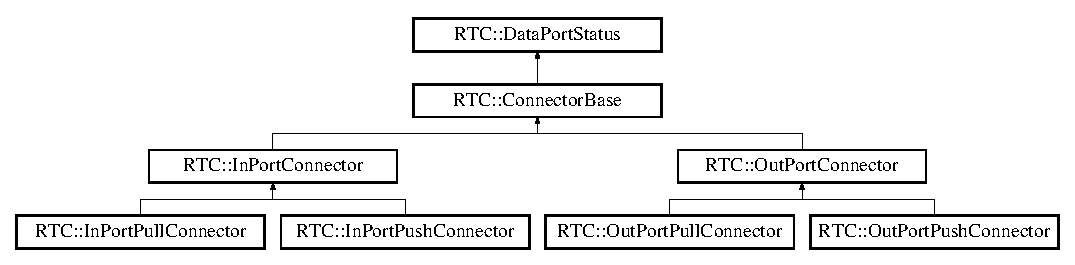
\includegraphics[height=3.11111cm]{classRTC_1_1ConnectorBase}
\end{center}
\end{figure}
\subsection*{Public メソッド}
\begin{DoxyCompactItemize}
\item 
virtual {\bf $\sim$ConnectorBase} ()
\begin{DoxyCompactList}\small\item\em デストラクタ \item\end{DoxyCompactList}\item 
virtual const {\bf ConnectorInfo} \& {\bf profile} ()=0
\begin{DoxyCompactList}\small\item\em \doxyref{Profile}{p.}{classProfile} 取得. \item\end{DoxyCompactList}\item 
virtual const char $\ast$ {\bf id} ()=0
\begin{DoxyCompactList}\small\item\em Connector ID 取得. \item\end{DoxyCompactList}\item 
virtual const char $\ast$ {\bf name} ()=0
\begin{DoxyCompactList}\small\item\em Connector 名取得. \item\end{DoxyCompactList}\item 
virtual ReturnCode {\bf disconnect} ()=0
\begin{DoxyCompactList}\small\item\em 接続解除関数 \item\end{DoxyCompactList}\item 
virtual {\bf CdrBufferBase} $\ast$ {\bf getBuffer} ()=0
\begin{DoxyCompactList}\small\item\em Buffer を取得する. \item\end{DoxyCompactList}\item 
virtual void {\bf activate} ()=0
\begin{DoxyCompactList}\small\item\em アクティブ化 \item\end{DoxyCompactList}\item 
virtual void {\bf deactivate} ()=0
\begin{DoxyCompactList}\small\item\em 非アクティブ化 \item\end{DoxyCompactList}\end{DoxyCompactItemize}


\subsection{説明}
Connector 基底クラス. InPort/OutPort, Push/Pull 各種 Connector を派生させるための 基底クラス。

\begin{DoxySince}{から}
1.0.0 
\end{DoxySince}


\subsection{コンストラクタとデストラクタ}
\index{RTC::ConnectorBase@{RTC::ConnectorBase}!$\sim$ConnectorBase@{$\sim$ConnectorBase}}
\index{$\sim$ConnectorBase@{$\sim$ConnectorBase}!RTC::ConnectorBase@{RTC::ConnectorBase}}
\subsubsection[{$\sim$ConnectorBase}]{\setlength{\rightskip}{0pt plus 5cm}virtual RTC::ConnectorBase::$\sim$ConnectorBase ()\hspace{0.3cm}{\ttfamily  [inline, virtual]}}\label{classRTC_1_1ConnectorBase_afa5e1e6f1924c4f6e90b1e7a2efd869e}


デストラクタ 



\subsection{関数}
\index{RTC::ConnectorBase@{RTC::ConnectorBase}!activate@{activate}}
\index{activate@{activate}!RTC::ConnectorBase@{RTC::ConnectorBase}}
\subsubsection[{activate}]{\setlength{\rightskip}{0pt plus 5cm}virtual void RTC::ConnectorBase::activate ()\hspace{0.3cm}{\ttfamily  [pure virtual]}}\label{classRTC_1_1ConnectorBase_a6f7f9ddd882546044f911d66aefee665}


アクティブ化 

このコネクタをアクティブ化する 

{\bf RTC::InPortPullConnector} \doxyref{}{p.}{classRTC_1_1InPortPullConnector_a0caf7d4d08dec18fd2973b39d2bc497d}, {\bf RTC::InPortPushConnector} \doxyref{}{p.}{classRTC_1_1InPortPushConnector_a5a34568fa4c67ad895e7842882077e30}, {\bf RTC::OutPortPullConnector} \doxyref{}{p.}{classRTC_1_1OutPortPullConnector_a4a2119db40dea439bc6da3eeeed11aa5}, と {\bf RTC::OutPortPushConnector} \doxyref{}{p.}{classRTC_1_1OutPortPushConnector_ad99dbf702d15a56b9d0b0deca3f8469a}で実装されています。

\index{RTC::ConnectorBase@{RTC::ConnectorBase}!deactivate@{deactivate}}
\index{deactivate@{deactivate}!RTC::ConnectorBase@{RTC::ConnectorBase}}
\subsubsection[{deactivate}]{\setlength{\rightskip}{0pt plus 5cm}virtual void RTC::ConnectorBase::deactivate ()\hspace{0.3cm}{\ttfamily  [pure virtual]}}\label{classRTC_1_1ConnectorBase_a8fe6a1bfe8d5ee586d51293b2bcf36d1}


非アクティブ化 

このコネクタを非アクティブ化する 

{\bf RTC::InPortPullConnector} \doxyref{}{p.}{classRTC_1_1InPortPullConnector_a1dcb7d9c9c4eb8e4667180f1da142788}, {\bf RTC::InPortPushConnector} \doxyref{}{p.}{classRTC_1_1InPortPushConnector_af93f9456bc93eba17fda8b2f0ceda313}, {\bf RTC::OutPortPullConnector} \doxyref{}{p.}{classRTC_1_1OutPortPullConnector_a2a681ec7dc8db477c34ce2bd84e1ac44}, と {\bf RTC::OutPortPushConnector} \doxyref{}{p.}{classRTC_1_1OutPortPushConnector_a5a3f57bca350504a903b10c2a57ac80b}で実装されています。

\index{RTC::ConnectorBase@{RTC::ConnectorBase}!disconnect@{disconnect}}
\index{disconnect@{disconnect}!RTC::ConnectorBase@{RTC::ConnectorBase}}
\subsubsection[{disconnect}]{\setlength{\rightskip}{0pt plus 5cm}virtual ReturnCode RTC::ConnectorBase::disconnect ()\hspace{0.3cm}{\ttfamily  [pure virtual]}}\label{classRTC_1_1ConnectorBase_a17b1e3bb26ccb844ef2952661977768c}


接続解除関数 

Connector が保持している接続を解除する 

{\bf RTC::InPortConnector} \doxyref{}{p.}{classRTC_1_1InPortConnector_a8677105bbf5ae5ed3e79dc3b057ea0b9}, {\bf RTC::InPortPullConnector} \doxyref{}{p.}{classRTC_1_1InPortPullConnector_a74e8c2fbfdbbacd1d3a67b4017b993df}, {\bf RTC::InPortPushConnector} \doxyref{}{p.}{classRTC_1_1InPortPushConnector_afb5920eabaa874b43bc900348a2fb2ad}, {\bf RTC::OutPortConnector} \doxyref{}{p.}{classRTC_1_1OutPortConnector_a0871d3168eb72d38b598cf862f1ac799}, {\bf RTC::OutPortPullConnector} \doxyref{}{p.}{classRTC_1_1OutPortPullConnector_aef4713815a7140da7c65b690c3a89256}, と {\bf RTC::OutPortPushConnector} \doxyref{}{p.}{classRTC_1_1OutPortPushConnector_ace1f7f9d47a8c2a31781a8cc1da828f0}で実装されています。

\index{RTC::ConnectorBase@{RTC::ConnectorBase}!getBuffer@{getBuffer}}
\index{getBuffer@{getBuffer}!RTC::ConnectorBase@{RTC::ConnectorBase}}
\subsubsection[{getBuffer}]{\setlength{\rightskip}{0pt plus 5cm}virtual {\bf CdrBufferBase}$\ast$ RTC::ConnectorBase::getBuffer ()\hspace{0.3cm}{\ttfamily  [pure virtual]}}\label{classRTC_1_1ConnectorBase_ad06710a5e9e1862ed50d4a4411c2927d}


Buffer を取得する. 

Connector が保持している Buffer を返す 

{\bf RTC::InPortConnector} \doxyref{}{p.}{classRTC_1_1InPortConnector_a7a2e6e83f1c50892632b5e23bf2f8ec6}, {\bf RTC::OutPortConnector} \doxyref{}{p.}{classRTC_1_1OutPortConnector_aed38944495c634d459bb0c06618f33a1}, {\bf RTC::OutPortPullConnector} \doxyref{}{p.}{classRTC_1_1OutPortPullConnector_a8b3df65ce00c96f9c4782653948b59d3}, と {\bf RTC::OutPortPushConnector} \doxyref{}{p.}{classRTC_1_1OutPortPushConnector_a5a04e7d25e944f89cbc5a323749887fd}で実装されています。

\index{RTC::ConnectorBase@{RTC::ConnectorBase}!id@{id}}
\index{id@{id}!RTC::ConnectorBase@{RTC::ConnectorBase}}
\subsubsection[{id}]{\setlength{\rightskip}{0pt plus 5cm}virtual const char$\ast$ RTC::ConnectorBase::id ()\hspace{0.3cm}{\ttfamily  [pure virtual]}}\label{classRTC_1_1ConnectorBase_ae2cc57833a7e28f0e605222ecb63e219}


Connector ID 取得. 

Connector ID を取得する 

{\bf RTC::InPortConnector} \doxyref{}{p.}{classRTC_1_1InPortConnector_af497212651998eaef0c38913d4762f52}, と {\bf RTC::OutPortConnector} \doxyref{}{p.}{classRTC_1_1OutPortConnector_ae59f1f12f25e2749c8c57db09a3b3aee}で実装されています。

\index{RTC::ConnectorBase@{RTC::ConnectorBase}!name@{name}}
\index{name@{name}!RTC::ConnectorBase@{RTC::ConnectorBase}}
\subsubsection[{name}]{\setlength{\rightskip}{0pt plus 5cm}virtual const char$\ast$ RTC::ConnectorBase::name ()\hspace{0.3cm}{\ttfamily  [pure virtual]}}\label{classRTC_1_1ConnectorBase_a73e002174dc02ec4830c624e7fd96b43}


Connector 名取得. 

Connector 名を取得する 

{\bf RTC::InPortConnector} \doxyref{}{p.}{classRTC_1_1InPortConnector_abb9dd2bf3f81d132a2a3eb4f31ff461d}, と {\bf RTC::OutPortConnector} \doxyref{}{p.}{classRTC_1_1OutPortConnector_a5c82fa5aa785b8b8272137355025c0a8}で実装されています。

\index{RTC::ConnectorBase@{RTC::ConnectorBase}!profile@{profile}}
\index{profile@{profile}!RTC::ConnectorBase@{RTC::ConnectorBase}}
\subsubsection[{profile}]{\setlength{\rightskip}{0pt plus 5cm}virtual const {\bf ConnectorInfo}\& RTC::ConnectorBase::profile ()\hspace{0.3cm}{\ttfamily  [pure virtual]}}\label{classRTC_1_1ConnectorBase_a8bd2e9cbd6a9341ec4c97416dcf981c7}


\doxyref{Profile}{p.}{classProfile} 取得. 

Connector \doxyref{Profile}{p.}{classProfile} を取得する 

{\bf RTC::InPortConnector} \doxyref{}{p.}{classRTC_1_1InPortConnector_ade653239f3932f5968ee818ecfd53354}, と {\bf RTC::OutPortConnector} \doxyref{}{p.}{classRTC_1_1OutPortConnector_a1c21b81e5dd176cd5f3723a8a0783936}で実装されています。


\section{クラス RTC::ConnectorDataListener}
\label{classRTC_1_1ConnectorDataListener}\index{RTC::ConnectorDataListener@{RTC::ConnectorDataListener}}


\doxyref{ConnectorDataListener}{p.}{classRTC_1_1ConnectorDataListener} クラス.  




{\ttfamily \#include $<$ConnectorListener.h$>$}

RTC::ConnectorDataListenerに対する継承グラフ\begin{figure}[H]
\begin{center}
\leavevmode
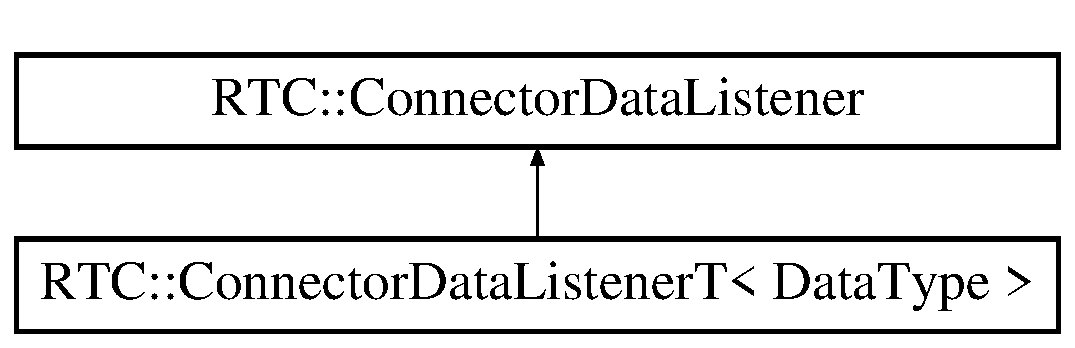
\includegraphics[height=2cm]{classRTC_1_1ConnectorDataListener}
\end{center}
\end{figure}
\subsection*{Public メソッド}
\begin{DoxyCompactItemize}
\item 
virtual {\bf $\sim$ConnectorDataListener} ()
\begin{DoxyCompactList}\small\item\em デストラクタ \item\end{DoxyCompactList}\item 
virtual void {\bf operator()} (const {\bf ConnectorInfo} \&info, const cdrMemoryStream \&data)=0
\begin{DoxyCompactList}\small\item\em 仮想コールバックメソッド \item\end{DoxyCompactList}\end{DoxyCompactItemize}
\subsection*{Static Public メソッド}
\begin{DoxyCompactItemize}
\item 
static const char $\ast$ {\bf toString} ({\bf ConnectorDataListenerType} type)
\begin{DoxyCompactList}\small\item\em ConnectorDataListenerType を文字列に変換. \item\end{DoxyCompactList}\end{DoxyCompactItemize}


\subsection{説明}
\doxyref{ConnectorDataListener}{p.}{classRTC_1_1ConnectorDataListener} クラス. データポートの Connector において発生する各種イベントに対するコー ルバックを実現するリスナクラスの基底クラス。

コアロジックがOutPortに対してデータ書き込み、InPort側でデータが取 得されるまでの間で発生する各種イベントをフックするコールバックを設 定することができる。なお、リスナークラスは2種類存在し、バッファフ ルや送信時のコールバックで、その時点で有効なデータをファンクタの引 数として受け取る \doxyref{ConnectorDataListener}{p.}{classRTC_1_1ConnectorDataListener} であり、もう一方はデータエ ンプティやバッファ読み込み時のタイムアウトなどデータが取得できない 場合などにコールされるファンクタの引数に何もとらならい ConnecotorListener がある。

データポートには、接続時にデータの送受信方法についてデータフロー型、 サブスクリプション型等を設定することができる。 ConnectorDaataListener/ConnectorListener はともに、様々なイベント に対するコールバックを設定することができるが、これらデータフロー型 およびサブスクリプション型の設定に応じて、利用可能なもの利用不可能 なものや、呼び出されるタイミングが異なる。 以下に、インターフェースがCORBA CDR型の場合のコールバック一覧を示す。

\doxyref{OutPort}{p.}{classRTC_1_1OutPort}:
\begin{DoxyItemize}
\item Push型: Subscription Typeによりさらにイベントの種類が分かれる。
\begin{DoxyItemize}
\item Flush: Flush型にはバッファがないため ON\_\-BUFFER 系のイベントは発生しない
\begin{DoxyItemize}
\item ON\_\-SEND
\item ON\_\-RECEIVED
\item ON\_\-RECEIVER\_\-FULL
\item ON\_\-RECEIVER\_\-TIMEOUT
\item ON\_\-RECEIVER\_\-ERROR
\item ON\_\-CONNECT
\item ON\_\-DISCONNECT
\end{DoxyItemize}
\item New型
\begin{DoxyItemize}
\item ON\_\-BUFFER\_\-WRITE
\item ON\_\-BUFFER\_\-FULL
\item ON\_\-BUFFER\_\-WRITE\_\-TIMEOUT
\item ON\_\-BUFFER\_\-OVERWRITE
\item ON\_\-BUFFER\_\-READ
\item ON\_\-SEND
\item ON\_\-RECEIVED
\item ON\_\-RECEIVER\_\-FULL
\item ON\_\-RECEIVER\_\-TIMEOUT
\item ON\_\-RECEIVER\_\-ERROR
\item ON\_\-SENDER\_\-ERROR
\item ON\_\-CONNECT
\item ON\_\-DISCONNECT
\end{DoxyItemize}
\item Periodic型
\begin{DoxyItemize}
\item ON\_\-BUFFER\_\-WRITE
\item ON\_\-BUFFER\_\-FULL
\item ON\_\-BUFFER\_\-WRITE\_\-TIMEOUT
\item ON\_\-BUFFER\_\-READ
\item ON\_\-SEND
\item ON\_\-RECEIVED
\item ON\_\-RECEIVER\_\-FULL
\item ON\_\-RECEIVER\_\-TIMEOUT
\item ON\_\-RECEIVER\_\-ERROR
\item ON\_\-BUFFER\_\-EMPTY
\item ON\_\-SENDER\_\-EMPTY
\item ON\_\-SENDER\_\-ERROR
\item ON\_\-CONNECT
\item ON\_\-DISCONNECT
\end{DoxyItemize}
\end{DoxyItemize}
\item Pull型
\begin{DoxyItemize}
\item ON\_\-BUFFER\_\-READ
\item ON\_\-SEND
\item ON\_\-BUFFER\_\-EMPTY
\item ON\_\-BUFFER\_\-READ\_\-TIMEOUT
\item ON\_\-SENDER\_\-EMPTY
\item ON\_\-SENDER\_\-TIMEOUT
\item ON\_\-SENDER\_\-ERROR
\item ON\_\-CONNECT
\item ON\_\-DISCONNECT
\end{DoxyItemize}
\end{DoxyItemize}

\doxyref{InPort}{p.}{classRTC_1_1InPort}:
\begin{DoxyItemize}
\item Push型:
\begin{DoxyItemize}
\item ON\_\-BUFFER\_\-WRITE
\item ON\_\-BUFFER\_\-FULL
\item ON\_\-BUFFER\_\-WRITE\_\-TIMEOUT
\item ON\_\-BUFFER\_\-WRITE\_\-OVERWRITE
\item ON\_\-RECEIVED
\item ON\_\-RECEIVER\_\-FULL
\item ON\_\-RECEIVER\_\-TIMEOUT
\item ON\_\-RECEIVER\_\-ERROR
\item ON\_\-CONNECT
\item ON\_\-DISCONNECT
\end{DoxyItemize}
\item Pull型
\begin{DoxyItemize}
\item ON\_\-CONNECT
\item ON\_\-DISCONNECT 
\end{DoxyItemize}
\end{DoxyItemize}

\subsection{コンストラクタとデストラクタ}
\index{RTC::ConnectorDataListener@{RTC::ConnectorDataListener}!$\sim$ConnectorDataListener@{$\sim$ConnectorDataListener}}
\index{$\sim$ConnectorDataListener@{$\sim$ConnectorDataListener}!RTC::ConnectorDataListener@{RTC::ConnectorDataListener}}
\subsubsection[{$\sim$ConnectorDataListener}]{\setlength{\rightskip}{0pt plus 5cm}virtual RTC::ConnectorDataListener::$\sim$ConnectorDataListener ()\hspace{0.3cm}{\ttfamily  [virtual]}}\label{classRTC_1_1ConnectorDataListener_add956ee4c385ddd1e8f49b6ce052999f}


デストラクタ 



\subsection{関数}
\index{RTC::ConnectorDataListener@{RTC::ConnectorDataListener}!operator()@{operator()}}
\index{operator()@{operator()}!RTC::ConnectorDataListener@{RTC::ConnectorDataListener}}
\subsubsection[{operator()}]{\setlength{\rightskip}{0pt plus 5cm}virtual void RTC::ConnectorDataListener::operator() (const {\bf ConnectorInfo} \& {\em info}, \/  const cdrMemoryStream \& {\em data})\hspace{0.3cm}{\ttfamily  [pure virtual]}}\label{classRTC_1_1ConnectorDataListener_a3306cb3544db5d164c5917adddbfc298}


仮想コールバックメソッド 

データポートの Connector において発生する各種イベントに対するコー ルバックメソッド 

{\bf RTC::ConnectorDataListenerT$<$ DataType $>$} \doxyref{}{p.}{classRTC_1_1ConnectorDataListenerT_a6d87ccd84018b4e5437336cbe7f9c72c}で実装されています。

\index{RTC::ConnectorDataListener@{RTC::ConnectorDataListener}!toString@{toString}}
\index{toString@{toString}!RTC::ConnectorDataListener@{RTC::ConnectorDataListener}}
\subsubsection[{toString}]{\setlength{\rightskip}{0pt plus 5cm}static const char$\ast$ RTC::ConnectorDataListener::toString ({\bf ConnectorDataListenerType} {\em type})\hspace{0.3cm}{\ttfamily  [inline, static]}}\label{classRTC_1_1ConnectorDataListener_ad626d18a31d3264d5c23cd55cd319fcb}


ConnectorDataListenerType を文字列に変換. 

ConnectorDataListenerType を文字列に変換する


\begin{DoxyParams}{引数}
\item[{\em type}]変換対象 ConnectorDataListenerType\end{DoxyParams}
\begin{DoxyReturn}{戻り値}
文字列変換結果 
\end{DoxyReturn}


参照先 RTC::CONNECTOR\_\-DATA\_\-LISTENER\_\-NUM.


\section{RTC::ConnectorDataListenerHolder Class Reference}
\label{classRTC_1_1ConnectorDataListenerHolder}\index{RTC::ConnectorDataListenerHolder@{RTC::ConnectorDataListenerHolder}}


\doxyref{ConnectorDataListener}{p.}{classRTC_1_1ConnectorDataListener} holder class.  




{\ttfamily \#include $<$ConnectorListener.h$>$}

\subsection*{Public Member Functions}
\begin{DoxyCompactItemize}
\item 
{\bf ConnectorDataListenerHolder} ()
\begin{DoxyCompactList}\small\item\em Constructor. \item\end{DoxyCompactList}\item 
virtual {\bf $\sim$ConnectorDataListenerHolder} ()
\begin{DoxyCompactList}\small\item\em Destructor. \item\end{DoxyCompactList}\item 
void {\bf addListener} ({\bf ConnectorDataListener} $\ast$listener, bool autoclean)
\begin{DoxyCompactList}\small\item\em Add the listener. \item\end{DoxyCompactList}\item 
void {\bf removeListener} ({\bf ConnectorDataListener} $\ast$listener)
\begin{DoxyCompactList}\small\item\em Remove the listener. \item\end{DoxyCompactList}\item 
void {\bf notify} (const {\bf ConnectorInfo} \&info, const cdrMemoryStream \&cdrdata)
\begin{DoxyCompactList}\small\item\em Notify listeners. \item\end{DoxyCompactList}\end{DoxyCompactItemize}


\subsection{Detailed Description}
\doxyref{ConnectorDataListener}{p.}{classRTC_1_1ConnectorDataListener} holder class. This class manages one ore more instances of \doxyref{ConnectorDataListener}{p.}{classRTC_1_1ConnectorDataListener} class. 

\subsection{Constructor \& Destructor Documentation}
\index{RTC::ConnectorDataListenerHolder@{RTC::ConnectorDataListenerHolder}!ConnectorDataListenerHolder@{ConnectorDataListenerHolder}}
\index{ConnectorDataListenerHolder@{ConnectorDataListenerHolder}!RTC::ConnectorDataListenerHolder@{RTC::ConnectorDataListenerHolder}}
\subsubsection[{ConnectorDataListenerHolder}]{\setlength{\rightskip}{0pt plus 5cm}RTC::ConnectorDataListenerHolder::ConnectorDataListenerHolder ()}\label{classRTC_1_1ConnectorDataListenerHolder_aa0c299c42ade0ce19b2ef5b70136034d}


Constructor. 

\index{RTC::ConnectorDataListenerHolder@{RTC::ConnectorDataListenerHolder}!$\sim$ConnectorDataListenerHolder@{$\sim$ConnectorDataListenerHolder}}
\index{$\sim$ConnectorDataListenerHolder@{$\sim$ConnectorDataListenerHolder}!RTC::ConnectorDataListenerHolder@{RTC::ConnectorDataListenerHolder}}
\subsubsection[{$\sim$ConnectorDataListenerHolder}]{\setlength{\rightskip}{0pt plus 5cm}virtual RTC::ConnectorDataListenerHolder::$\sim$ConnectorDataListenerHolder ()\hspace{0.3cm}{\ttfamily  [virtual]}}\label{classRTC_1_1ConnectorDataListenerHolder_a50ba55ec3f0ded808616e9c79aa63ef1}


Destructor. 



\subsection{Member Function Documentation}
\index{RTC::ConnectorDataListenerHolder@{RTC::ConnectorDataListenerHolder}!addListener@{addListener}}
\index{addListener@{addListener}!RTC::ConnectorDataListenerHolder@{RTC::ConnectorDataListenerHolder}}
\subsubsection[{addListener}]{\setlength{\rightskip}{0pt plus 5cm}void RTC::ConnectorDataListenerHolder::addListener ({\bf ConnectorDataListener} $\ast$ {\em listener}, \/  bool {\em autoclean})}\label{classRTC_1_1ConnectorDataListenerHolder_a37534a08dd65b6c1bb54776d21970995}


Add the listener. 

This method adds the listener.


\begin{DoxyParams}{Parameters}
\item[{\em listener}]Added listener \item[{\em autoclean}]true:The listener is deleted at the destructor., false:The listener is not deleted at the destructor. \end{DoxyParams}
\index{RTC::ConnectorDataListenerHolder@{RTC::ConnectorDataListenerHolder}!notify@{notify}}
\index{notify@{notify}!RTC::ConnectorDataListenerHolder@{RTC::ConnectorDataListenerHolder}}
\subsubsection[{notify}]{\setlength{\rightskip}{0pt plus 5cm}void RTC::ConnectorDataListenerHolder::notify (const {\bf ConnectorInfo} \& {\em info}, \/  const cdrMemoryStream \& {\em cdrdata})}\label{classRTC_1_1ConnectorDataListenerHolder_a44a647d9839d95c2c414a7d8737feb7b}


Notify listeners. 

This calls the Callback method of the registered listener.


\begin{DoxyParams}{Parameters}
\item[{\em info}]\doxyref{ConnectorInfo}{p.}{classRTC_1_1ConnectorInfo} \item[{\em cdrdata}]Data \end{DoxyParams}
\index{RTC::ConnectorDataListenerHolder@{RTC::ConnectorDataListenerHolder}!removeListener@{removeListener}}
\index{removeListener@{removeListener}!RTC::ConnectorDataListenerHolder@{RTC::ConnectorDataListenerHolder}}
\subsubsection[{removeListener}]{\setlength{\rightskip}{0pt plus 5cm}void RTC::ConnectorDataListenerHolder::removeListener ({\bf ConnectorDataListener} $\ast$ {\em listener})}\label{classRTC_1_1ConnectorDataListenerHolder_a966d7887d2168f2b7a5cc2b1a721ae8d}


Remove the listener. 

This method removes the listener.


\begin{DoxyParams}{Parameters}
\item[{\em listener}]Removed listener \end{DoxyParams}

\section{RTC::ConnectorDataListenerT$<$ DataType $>$ Class Template Reference}
\label{classRTC_1_1ConnectorDataListenerT}\index{RTC::ConnectorDataListenerT@{RTC::ConnectorDataListenerT}}


\doxyref{ConnectorDataListenerT}{p.}{classRTC_1_1ConnectorDataListenerT} class.  




{\ttfamily \#include $<$ConnectorListener.h$>$}

Inheritance diagram for RTC::ConnectorDataListenerT$<$ DataType $>$:\begin{figure}[H]
\begin{center}
\leavevmode
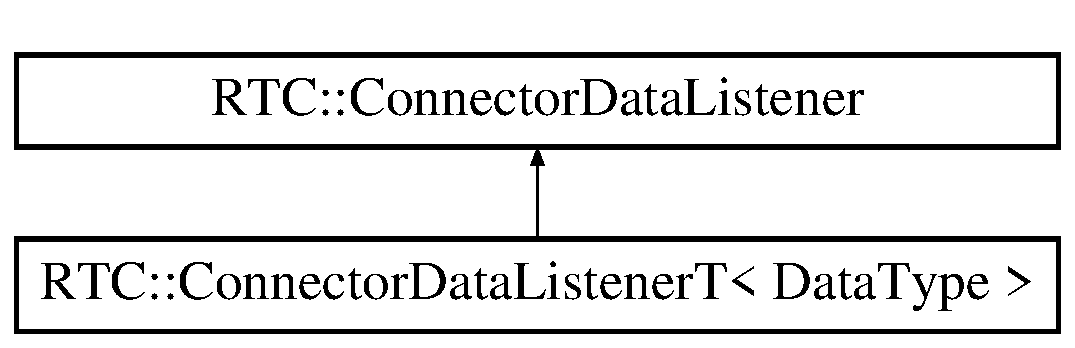
\includegraphics[height=2cm]{classRTC_1_1ConnectorDataListenerT}
\end{center}
\end{figure}
\subsection*{Public Member Functions}
\begin{DoxyCompactItemize}
\item 
virtual {\bf $\sim$ConnectorDataListenerT} ()
\begin{DoxyCompactList}\small\item\em Destructor. \item\end{DoxyCompactList}\item 
virtual void {\bf operator()} (const {\bf ConnectorInfo} \&info, const cdrMemoryStream \&cdrdata)
\begin{DoxyCompactList}\small\item\em Callback method. \item\end{DoxyCompactList}\item 
virtual void {\bf operator()} (const {\bf ConnectorInfo} \&info, const DataType \&data)=0
\begin{DoxyCompactList}\small\item\em Virtual Callback method. \item\end{DoxyCompactList}\end{DoxyCompactItemize}


\subsection{Detailed Description}
\subsubsection*{template$<$class DataType$>$ class RTC::ConnectorDataListenerT$<$ DataType $>$}

\doxyref{ConnectorDataListenerT}{p.}{classRTC_1_1ConnectorDataListenerT} class. This class is abstract base class for listener classes that provides callbacks for various events in the data port's connectors.

This class template can have practical data types that are used as typed variable for DataPort as an argument of template instead of cdrMemoryStream. 

\subsection{Constructor \& Destructor Documentation}
\index{RTC::ConnectorDataListenerT@{RTC::ConnectorDataListenerT}!$\sim$ConnectorDataListenerT@{$\sim$ConnectorDataListenerT}}
\index{$\sim$ConnectorDataListenerT@{$\sim$ConnectorDataListenerT}!RTC::ConnectorDataListenerT@{RTC::ConnectorDataListenerT}}
\subsubsection[{$\sim$ConnectorDataListenerT}]{\setlength{\rightskip}{0pt plus 5cm}template$<$class DataType $>$ virtual {\bf RTC::ConnectorDataListenerT}$<$ DataType $>$::$\sim${\bf ConnectorDataListenerT} ()\hspace{0.3cm}{\ttfamily  [inline, virtual]}}\label{classRTC_1_1ConnectorDataListenerT_a7e07ce2456ad559f78b24467a22ce4ab}


Destructor. 



\subsection{Member Function Documentation}
\index{RTC::ConnectorDataListenerT@{RTC::ConnectorDataListenerT}!operator()@{operator()}}
\index{operator()@{operator()}!RTC::ConnectorDataListenerT@{RTC::ConnectorDataListenerT}}
\subsubsection[{operator()}]{\setlength{\rightskip}{0pt plus 5cm}template$<$class DataType $>$ virtual void {\bf RTC::ConnectorDataListenerT}$<$ DataType $>$::operator() (const {\bf ConnectorInfo} \& {\em info}, \/  const DataType \& {\em data})\hspace{0.3cm}{\ttfamily  [pure virtual]}}\label{classRTC_1_1ConnectorDataListenerT_a74a7cf49e64721834da69c82e1769d3f}


Virtual Callback method. 

This method invokes the callback method of \doxyref{ConnectorDataListenerT}{p.}{classRTC_1_1ConnectorDataListenerT}. Data is converted into the variable type used in DataPort. \index{RTC::ConnectorDataListenerT@{RTC::ConnectorDataListenerT}!operator()@{operator()}}
\index{operator()@{operator()}!RTC::ConnectorDataListenerT@{RTC::ConnectorDataListenerT}}
\subsubsection[{operator()}]{\setlength{\rightskip}{0pt plus 5cm}template$<$class DataType $>$ virtual void {\bf RTC::ConnectorDataListenerT}$<$ DataType $>$::operator() (const {\bf ConnectorInfo} \& {\em info}, \/  const cdrMemoryStream \& {\em cdrdata})\hspace{0.3cm}{\ttfamily  [inline, virtual]}}\label{classRTC_1_1ConnectorDataListenerT_a6d87ccd84018b4e5437336cbe7f9c72c}


Callback method. 

This method invokes the callback method of \doxyref{ConnectorDataListenerT}{p.}{classRTC_1_1ConnectorDataListenerT}. Data is converted into the variable type used in DataPort.


\begin{DoxyParams}{Parameters}
\item[{\em info}]\doxyref{ConnectorInfo}{p.}{classRTC_1_1ConnectorInfo} \item[{\em cdrdata}]Data of cdrMemoryStream type \end{DoxyParams}


Implements {\bf RTC::ConnectorDataListener} \doxyref{}{p.}{classRTC_1_1ConnectorDataListener_a3306cb3544db5d164c5917adddbfc298}.



References coil::Properties::getProperty(), coil::normalize(), RTC::ConnectorInfo::properties, and coil::split().


\section{RTC::ConnectorInfo Class Reference}
\label{classRTC_1_1ConnectorInfo}\index{RTC::ConnectorInfo@{RTC::ConnectorInfo}}


{\ttfamily \#include $<$ConnectorBase.h$>$}

\subsection*{Public Member Functions}
\begin{DoxyCompactItemize}
\item 
{\bf ConnectorInfo} (const char $\ast$name\_\-, const char $\ast$id\_\-, {\bf coil::vstring} ports\_\-, {\bf coil::Properties} properties\_\-)
\begin{DoxyCompactList}\small\item\em Constructor. \item\end{DoxyCompactList}\item 
{\bf ConnectorInfo} ()
\begin{DoxyCompactList}\small\item\em Constructor. \item\end{DoxyCompactList}\end{DoxyCompactItemize}
\subsection*{Public Attributes}
\begin{DoxyCompactItemize}
\item 
std::string {\bf name}
\begin{DoxyCompactList}\small\item\em Connection name. \item\end{DoxyCompactList}\item 
std::string {\bf id}
\begin{DoxyCompactList}\small\item\em ConnectionID. \item\end{DoxyCompactList}\item 
{\bf coil::vstring} {\bf ports}
\begin{DoxyCompactList}\small\item\em Connection ports. \item\end{DoxyCompactList}\item 
{\bf coil::Properties} {\bf properties}
\begin{DoxyCompactList}\small\item\em Connection properties. \item\end{DoxyCompactList}\end{DoxyCompactItemize}


\subsection{Constructor \& Destructor Documentation}
\index{RTC::ConnectorInfo@{RTC::ConnectorInfo}!ConnectorInfo@{ConnectorInfo}}
\index{ConnectorInfo@{ConnectorInfo}!RTC::ConnectorInfo@{RTC::ConnectorInfo}}
\subsubsection[{ConnectorInfo}]{\setlength{\rightskip}{0pt plus 5cm}RTC::ConnectorInfo::ConnectorInfo (const char $\ast$ {\em name\_\-}, \/  const char $\ast$ {\em id\_\-}, \/  {\bf coil::vstring} {\em ports\_\-}, \/  {\bf coil::Properties} {\em properties\_\-})\hspace{0.3cm}{\ttfamily  [inline]}}\label{classRTC_1_1ConnectorInfo_af4d6c063f07b31ee3ee79028cffdf1f8}


Constructor. 

Constructor


\begin{DoxyParams}{Parameters}
\item[{\em name\_\-}]connection name \item[{\em id\_\-}]connection ID \item[{\em ports\_\-}]connection Ports \item[{\em properties\_\-}]connection properties \end{DoxyParams}
\index{RTC::ConnectorInfo@{RTC::ConnectorInfo}!ConnectorInfo@{ConnectorInfo}}
\index{ConnectorInfo@{ConnectorInfo}!RTC::ConnectorInfo@{RTC::ConnectorInfo}}
\subsubsection[{ConnectorInfo}]{\setlength{\rightskip}{0pt plus 5cm}RTC::ConnectorInfo::ConnectorInfo ()\hspace{0.3cm}{\ttfamily  [inline]}}\label{classRTC_1_1ConnectorInfo_a35326894f5367b961eadccf0e8da98c3}


Constructor. 

Constructor 

\subsection{Member Data Documentation}
\index{RTC::ConnectorInfo@{RTC::ConnectorInfo}!id@{id}}
\index{id@{id}!RTC::ConnectorInfo@{RTC::ConnectorInfo}}
\subsubsection[{id}]{\setlength{\rightskip}{0pt plus 5cm}std::string {\bf RTC::ConnectorInfo::id}}\label{classRTC_1_1ConnectorInfo_ab5bef6c4b11d73cc51d8949950a4e969}


ConnectionID. 

\index{RTC::ConnectorInfo@{RTC::ConnectorInfo}!name@{name}}
\index{name@{name}!RTC::ConnectorInfo@{RTC::ConnectorInfo}}
\subsubsection[{name}]{\setlength{\rightskip}{0pt plus 5cm}std::string {\bf RTC::ConnectorInfo::name}}\label{classRTC_1_1ConnectorInfo_a7cf9f73a6b055dc52f62d6b7cd92e97d}


Connection name. 

\index{RTC::ConnectorInfo@{RTC::ConnectorInfo}!ports@{ports}}
\index{ports@{ports}!RTC::ConnectorInfo@{RTC::ConnectorInfo}}
\subsubsection[{ports}]{\setlength{\rightskip}{0pt plus 5cm}{\bf coil::vstring} {\bf RTC::ConnectorInfo::ports}}\label{classRTC_1_1ConnectorInfo_a2424113611e0cdd498f526ac58f67fba}


Connection ports. 

\index{RTC::ConnectorInfo@{RTC::ConnectorInfo}!properties@{properties}}
\index{properties@{properties}!RTC::ConnectorInfo@{RTC::ConnectorInfo}}
\subsubsection[{properties}]{\setlength{\rightskip}{0pt plus 5cm}{\bf coil::Properties} {\bf RTC::ConnectorInfo::properties}}\label{classRTC_1_1ConnectorInfo_a480039d0964d885b3cac8e6d1ec64584}


Connection properties. 



Referenced by RTC::ConnectorDataListenerT$<$ DataType $>$::operator()().


\section{クラス RTC::ConnectorListener}
\label{classRTC_1_1ConnectorListener}\index{RTC::ConnectorListener@{RTC::ConnectorListener}}


\doxyref{ConnectorListener}{p.}{classRTC_1_1ConnectorListener} クラス.  




{\ttfamily \#include $<$ConnectorListener.h$>$}

\subsection*{Public メソッド}
\begin{DoxyCompactItemize}
\item 
virtual {\bf $\sim$ConnectorListener} ()
\begin{DoxyCompactList}\small\item\em デストラクタ \item\end{DoxyCompactList}\item 
virtual void {\bf operator()} (const {\bf ConnectorInfo} \&info)=0
\begin{DoxyCompactList}\small\item\em 仮想コールバックメソッド \item\end{DoxyCompactList}\end{DoxyCompactItemize}
\subsection*{Static Public メソッド}
\begin{DoxyCompactItemize}
\item 
static const char $\ast$ {\bf toString} ({\bf ConnectorListenerType} type)
\begin{DoxyCompactList}\small\item\em ConnectorListenerType を文字列に変換. \item\end{DoxyCompactList}\end{DoxyCompactItemize}


\subsection{説明}
\doxyref{ConnectorListener}{p.}{classRTC_1_1ConnectorListener} クラス. データポートの Connector において発生する各種イベントに対するコー ルバックを実現するリスナクラスの基底クラス。

コアロジックがOutPortに対してデータ書き込み、InPort側でデータが取 得されるまでの間で発生する各種イベントをフックするコールバックを設 定することができる。なお、リスナークラスは2種類存在し、バッファフ ルや送信時のコールバックで、その時点で有効なデータをファンクタの引 数として受け取る \doxyref{ConnectorDataListener}{p.}{classRTC_1_1ConnectorDataListener} であり、もう一方はデータエ ンプティやバッファ読み込み時のタイムアウトなどデータが取得できない 場合などにコールされるファンクタの引数に何もとらならい ConnecotorListener がある。

データポートには、接続時にデータの送受信方法についてデータフロー型、 サブスクリプション型等を設定することができる。 ConnectorDaataListener/ConnectorListener は共にに、様々なイベント に対するコールバックを設定することができるが、これらデータフロー型 およびサブスクリプション型の設定に応じて、利用できるもの、できない もの、また呼び出されるタイミングが異なる。以下に、インターフェース がCORBA CDR型の場合のコールバック一覧を示す。

\doxyref{OutPort}{p.}{classRTC_1_1OutPort}:
\begin{DoxyItemize}
\item Push型: Subscription Typeによりさらにイベントの種類が分かれる。
\begin{DoxyItemize}
\item Flush: Flush型にはバッファがないため ON\_\-BUFFER 系のイベントは発生しない
\begin{DoxyItemize}
\item ON\_\-SEND
\item ON\_\-RECEIVED
\item ON\_\-RECEIVER\_\-FULL
\item ON\_\-RECEIVER\_\-TIMEOUT
\item ON\_\-RECEIVER\_\-ERROR
\item ON\_\-CONNECT
\item ON\_\-DISCONNECT
\end{DoxyItemize}
\item New型
\begin{DoxyItemize}
\item ON\_\-BUFFER\_\-WRITE
\item ON\_\-BUFFER\_\-FULL
\item ON\_\-BUFFER\_\-WRITE\_\-TIMEOUT
\item ON\_\-BUFFER\_\-OVERWRITE
\item ON\_\-BUFFER\_\-READ
\item ON\_\-SEND
\item ON\_\-RECEIVED
\item ON\_\-RECEIVER\_\-FULL
\item ON\_\-RECEIVER\_\-TIMEOUT
\item ON\_\-RECEIVER\_\-ERROR
\item ON\_\-SENDER\_\-ERROR
\item ON\_\-CONNECT
\item ON\_\-DISCONNECT
\end{DoxyItemize}
\item Periodic型
\begin{DoxyItemize}
\item ON\_\-BUFFER\_\-WRITE
\item ON\_\-BUFFER\_\-FULL
\item ON\_\-BUFFER\_\-WRITE\_\-TIMEOUT
\item ON\_\-BUFFER\_\-READ
\item ON\_\-SEND
\item ON\_\-RECEIVED
\item ON\_\-RECEIVER\_\-FULL
\item ON\_\-RECEIVER\_\-TIMEOUT
\item ON\_\-RECEIVER\_\-ERROR
\item ON\_\-BUFFER\_\-EMPTY
\item ON\_\-SENDER\_\-EMPTY
\item ON\_\-SENDER\_\-ERROR
\item ON\_\-CONNECT
\item ON\_\-DISCONNECT
\end{DoxyItemize}
\end{DoxyItemize}
\item Pull型
\begin{DoxyItemize}
\item ON\_\-BUFFER\_\-READ
\item ON\_\-SEND
\item ON\_\-BUFFER\_\-EMPTY
\item ON\_\-BUFFER\_\-READ\_\-TIMEOUT
\item ON\_\-SENDER\_\-EMPTY
\item ON\_\-SENDER\_\-TIMEOUT
\item ON\_\-SENDER\_\-ERROR
\item ON\_\-CONNECT
\item ON\_\-DISCONNECT
\end{DoxyItemize}
\end{DoxyItemize}

\doxyref{InPort}{p.}{classRTC_1_1InPort}:
\begin{DoxyItemize}
\item Push型:
\begin{DoxyItemize}
\item ON\_\-BUFFER\_\-WRITE
\item ON\_\-BUFFER\_\-FULL
\item ON\_\-BUFFER\_\-WRITE\_\-TIMEOUT
\item ON\_\-BUFFER\_\-WRITE\_\-OVERWRITE
\item ON\_\-RECEIVED
\item ON\_\-RECEIVER\_\-FULL
\item ON\_\-RECEIVER\_\-TIMEOUT
\item ON\_\-RECEIVER\_\-ERROR
\item ON\_\-CONNECT
\item ON\_\-DISCONNECT
\end{DoxyItemize}
\item Pull型
\begin{DoxyItemize}
\item ON\_\-CONNECT
\item ON\_\-DISCONNECT 
\end{DoxyItemize}
\end{DoxyItemize}

\subsection{コンストラクタとデストラクタ}
\index{RTC::ConnectorListener@{RTC::ConnectorListener}!$\sim$ConnectorListener@{$\sim$ConnectorListener}}
\index{$\sim$ConnectorListener@{$\sim$ConnectorListener}!RTC::ConnectorListener@{RTC::ConnectorListener}}
\subsubsection[{$\sim$ConnectorListener}]{\setlength{\rightskip}{0pt plus 5cm}virtual RTC::ConnectorListener::$\sim$ConnectorListener ()\hspace{0.3cm}{\ttfamily  [virtual]}}\label{classRTC_1_1ConnectorListener_a023c28d2f4ce8fd10ac1990c914bb0e3}


デストラクタ 



\subsection{関数}
\index{RTC::ConnectorListener@{RTC::ConnectorListener}!operator()@{operator()}}
\index{operator()@{operator()}!RTC::ConnectorListener@{RTC::ConnectorListener}}
\subsubsection[{operator()}]{\setlength{\rightskip}{0pt plus 5cm}virtual void RTC::ConnectorListener::operator() (const {\bf ConnectorInfo} \& {\em info})\hspace{0.3cm}{\ttfamily  [pure virtual]}}\label{classRTC_1_1ConnectorListener_a4ad75b245ee498d3b4e037f6acbf9f75}


仮想コールバックメソッド 

データポートの Connector において発生する各種イベントに対するコー ルバックメソッド \index{RTC::ConnectorListener@{RTC::ConnectorListener}!toString@{toString}}
\index{toString@{toString}!RTC::ConnectorListener@{RTC::ConnectorListener}}
\subsubsection[{toString}]{\setlength{\rightskip}{0pt plus 5cm}static const char$\ast$ RTC::ConnectorListener::toString ({\bf ConnectorListenerType} {\em type})\hspace{0.3cm}{\ttfamily  [inline, static]}}\label{classRTC_1_1ConnectorListener_a3e0396e710d6450413672e6eb232a386}


ConnectorListenerType を文字列に変換. 

ConnectorListenerType を文字列に変換する


\begin{DoxyParams}{引数}
\item[{\em type}]変換対象 ConnectorListenerType\end{DoxyParams}
\begin{DoxyReturn}{戻り値}
文字列変換結果 
\end{DoxyReturn}


参照先 RTC::CONNECTOR\_\-LISTENER\_\-NUM.


\section{クラス RTC::ConnectorListenerHolder}
\label{classRTC_1_1ConnectorListenerHolder}\index{RTC::ConnectorListenerHolder@{RTC::ConnectorListenerHolder}}


\doxyref{ConnectorListener}{p.}{classRTC_1_1ConnectorListener} ホルダクラス.  




{\ttfamily \#include $<$ConnectorListener.h$>$}

\subsection*{Public メソッド}
\begin{DoxyCompactItemize}
\item 
{\bf ConnectorListenerHolder} ()
\begin{DoxyCompactList}\small\item\em コンストラクタ \item\end{DoxyCompactList}\item 
virtual {\bf $\sim$ConnectorListenerHolder} ()
\begin{DoxyCompactList}\small\item\em デストラクタ \item\end{DoxyCompactList}\item 
void {\bf addListener} ({\bf ConnectorListener} $\ast$listener, bool autoclean)
\begin{DoxyCompactList}\small\item\em リスナーの追加 \item\end{DoxyCompactList}\item 
void {\bf removeListener} ({\bf ConnectorListener} $\ast$listener)
\begin{DoxyCompactList}\small\item\em リスナーの削除 \item\end{DoxyCompactList}\item 
void {\bf notify} (const {\bf ConnectorInfo} \&info)
\begin{DoxyCompactList}\small\item\em リスナーへ通知する \item\end{DoxyCompactList}\end{DoxyCompactItemize}


\subsection{説明}
\doxyref{ConnectorListener}{p.}{classRTC_1_1ConnectorListener} ホルダクラス. 複数の \doxyref{ConnectorListener}{p.}{classRTC_1_1ConnectorListener} を保持し管理するクラス。 

\subsection{コンストラクタとデストラクタ}
\index{RTC::ConnectorListenerHolder@{RTC::ConnectorListenerHolder}!ConnectorListenerHolder@{ConnectorListenerHolder}}
\index{ConnectorListenerHolder@{ConnectorListenerHolder}!RTC::ConnectorListenerHolder@{RTC::ConnectorListenerHolder}}
\subsubsection[{ConnectorListenerHolder}]{\setlength{\rightskip}{0pt plus 5cm}RTC::ConnectorListenerHolder::ConnectorListenerHolder ()}\label{classRTC_1_1ConnectorListenerHolder_ab62f009d890220d946a8c5f1da16ba1d}


コンストラクタ 

\index{RTC::ConnectorListenerHolder@{RTC::ConnectorListenerHolder}!$\sim$ConnectorListenerHolder@{$\sim$ConnectorListenerHolder}}
\index{$\sim$ConnectorListenerHolder@{$\sim$ConnectorListenerHolder}!RTC::ConnectorListenerHolder@{RTC::ConnectorListenerHolder}}
\subsubsection[{$\sim$ConnectorListenerHolder}]{\setlength{\rightskip}{0pt plus 5cm}virtual RTC::ConnectorListenerHolder::$\sim$ConnectorListenerHolder ()\hspace{0.3cm}{\ttfamily  [virtual]}}\label{classRTC_1_1ConnectorListenerHolder_aab740e6b9f132c8cec547b377a38afa5}


デストラクタ 



\subsection{関数}
\index{RTC::ConnectorListenerHolder@{RTC::ConnectorListenerHolder}!addListener@{addListener}}
\index{addListener@{addListener}!RTC::ConnectorListenerHolder@{RTC::ConnectorListenerHolder}}
\subsubsection[{addListener}]{\setlength{\rightskip}{0pt plus 5cm}void RTC::ConnectorListenerHolder::addListener ({\bf ConnectorListener} $\ast$ {\em listener}, \/  bool {\em autoclean})}\label{classRTC_1_1ConnectorListenerHolder_a4a864412484c141ee173fa2840b1cfa1}


リスナーの追加 

リスナーを追加する。


\begin{DoxyParams}{引数}
\item[{\em listener}]追加するリスナ \item[{\em autoclean}]true:デストラクタで削除する, false:デストラクタで削除しない \end{DoxyParams}
\index{RTC::ConnectorListenerHolder@{RTC::ConnectorListenerHolder}!notify@{notify}}
\index{notify@{notify}!RTC::ConnectorListenerHolder@{RTC::ConnectorListenerHolder}}
\subsubsection[{notify}]{\setlength{\rightskip}{0pt plus 5cm}void RTC::ConnectorListenerHolder::notify (const {\bf ConnectorInfo} \& {\em info})}\label{classRTC_1_1ConnectorListenerHolder_a4c1522a804f3bdcab7dafeb0cca1e859}


リスナーへ通知する 

登録されているリスナのコールバックメソッドを呼び出す。


\begin{DoxyParams}{引数}
\item[{\em info}]\doxyref{ConnectorInfo}{p.}{classRTC_1_1ConnectorInfo} \end{DoxyParams}
\index{RTC::ConnectorListenerHolder@{RTC::ConnectorListenerHolder}!removeListener@{removeListener}}
\index{removeListener@{removeListener}!RTC::ConnectorListenerHolder@{RTC::ConnectorListenerHolder}}
\subsubsection[{removeListener}]{\setlength{\rightskip}{0pt plus 5cm}void RTC::ConnectorListenerHolder::removeListener ({\bf ConnectorListener} $\ast$ {\em listener})}\label{classRTC_1_1ConnectorListenerHolder_abd64fdf79758520c8b65f303225b27aa}


リスナーの削除 

リスナを削除する。


\begin{DoxyParams}{引数}
\item[{\em listener}]削除するリスナ \end{DoxyParams}

\section{クラス RTC::ConnectorListeners}
\label{classRTC_1_1ConnectorListeners}\index{RTC::ConnectorListeners@{RTC::ConnectorListeners}}


\doxyref{ConnectorListeners}{p.}{classRTC_1_1ConnectorListeners} クラス.  




{\ttfamily \#include $<$ConnectorListener.h$>$}

\subsection*{Public 変数}
\begin{DoxyCompactItemize}
\item 
{\bf ConnectorDataListenerHolder} {\bf connectorData\_\-} [CONNECTOR\_\-DATA\_\-LISTENER\_\-NUM]
\begin{DoxyCompactList}\small\item\em ConnectorDataListenerTypeリスナ配列 ConnectorDataListenerTypeリスナを格納. \item\end{DoxyCompactList}\item 
{\bf ConnectorListenerHolder} {\bf connector\_\-} [CONNECTOR\_\-LISTENER\_\-NUM]
\begin{DoxyCompactList}\small\item\em ConnectorListenerTypeリスナ配列 ConnectorListenerTypeリスナを格納. \item\end{DoxyCompactList}\end{DoxyCompactItemize}


\subsection{説明}
\doxyref{ConnectorListeners}{p.}{classRTC_1_1ConnectorListeners} クラス. 

\subsection{変数}
\index{RTC::ConnectorListeners@{RTC::ConnectorListeners}!connector\_\-@{connector\_\-}}
\index{connector\_\-@{connector\_\-}!RTC::ConnectorListeners@{RTC::ConnectorListeners}}
\subsubsection[{connector\_\-}]{\setlength{\rightskip}{0pt plus 5cm}{\bf ConnectorListenerHolder} {\bf RTC::ConnectorListeners::connector\_\-}[CONNECTOR\_\-LISTENER\_\-NUM]}\label{classRTC_1_1ConnectorListeners_a3b8bf4c15ef100a65edc0291063a5f04}


ConnectorListenerTypeリスナ配列 ConnectorListenerTypeリスナを格納. 

\index{RTC::ConnectorListeners@{RTC::ConnectorListeners}!connectorData\_\-@{connectorData\_\-}}
\index{connectorData\_\-@{connectorData\_\-}!RTC::ConnectorListeners@{RTC::ConnectorListeners}}
\subsubsection[{connectorData\_\-}]{\setlength{\rightskip}{0pt plus 5cm}{\bf ConnectorDataListenerHolder} {\bf RTC::ConnectorListeners::connectorData\_\-}[CONNECTOR\_\-DATA\_\-LISTENER\_\-NUM]}\label{classRTC_1_1ConnectorListeners_a32de5fe33a2924c37e95ed82f662738e}


ConnectorDataListenerTypeリスナ配列 ConnectorDataListenerTypeリスナを格納. 


\section{Consumer Class Reference}
\label{classConsumer}\index{Consumer@{Consumer}}


Placeholder template class to hold remote object reference.  




{\ttfamily \#include $<$CorbaConsumer.h$>$}



\subsection{Detailed Description}
Placeholder template class to hold remote object reference. This class holds a type of object that given by template parameter. For internal use, \_\-ptr type and \_\-var type should be given as template parameter. (Please refere the following notation.)

Note: ObjectTypePtr's default value is defined as ObjectType::\_\-ptr\_\-type, although \_\-ptr\_\-type is not defined as normative type. However, omniORB, TAO, MICO, ORBit, ORBacus define \_\-ptr\_\-type and \_\-var\_\-type as \_\-ptr type and \_\-var type in stub code. Usually, you don't need to specify 2nd and 3rd template arguments.

\begin{DoxySince}{Since}
0.4.0 
\end{DoxySince}

\section{ConsumerBase Class Reference}
\label{classConsumerBase}\index{ConsumerBase@{ConsumerBase}}


Placeholder base class to hold remote object reference.  




{\ttfamily \#include $<$CorbaConsumer.h$>$}



\subsection{Detailed Description}
Placeholder base class to hold remote object reference. A base class for consumer implementation when chose CORBA as a communication tool.

\begin{DoxySince}{Since}
0.4.0 
\end{DoxySince}

\section{RTC::CorbaConsumer$<$ ObjectType, ObjectTypePtr, ObjectTypeVar $>$ Class Template Reference}
\label{classRTC_1_1CorbaConsumer}\index{RTC::CorbaConsumer@{RTC::CorbaConsumer}}


{\ttfamily \#include $<$CorbaConsumer.h$>$}

Inheritance diagram for RTC::CorbaConsumer$<$ ObjectType, ObjectTypePtr, ObjectTypeVar $>$:\begin{figure}[H]
\begin{center}
\leavevmode
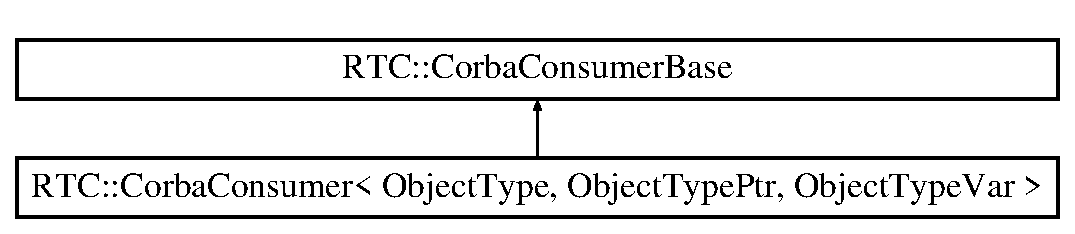
\includegraphics[height=2cm]{classRTC_1_1CorbaConsumer}
\end{center}
\end{figure}
\subsection*{Public Member Functions}
\begin{DoxyCompactItemize}
\item 
{\bf CorbaConsumer} ()
\begin{DoxyCompactList}\small\item\em Consructor. \item\end{DoxyCompactList}\item 
{\bf CorbaConsumer} (const {\bf CorbaConsumer} \&x)
\begin{DoxyCompactList}\small\item\em Copy constructor. \item\end{DoxyCompactList}\item 
{\bf CorbaConsumer} \& {\bf operator=} (const {\bf CorbaConsumer} \&x)
\begin{DoxyCompactList}\small\item\em Assignment operator. \item\end{DoxyCompactList}\item 
void {\bf swap} ({\bf CorbaConsumer} \&x)
\item 
virtual {\bf $\sim$CorbaConsumer} (void)
\begin{DoxyCompactList}\small\item\em Virtual destructor. \item\end{DoxyCompactList}\item 
virtual bool {\bf setObject} (CORBA::Object\_\-ptr obj)
\begin{DoxyCompactList}\small\item\em Set Object. \item\end{DoxyCompactList}\item 
ObjectTypePtr {\bf \_\-ptr} ()
\begin{DoxyCompactList}\small\item\em Get Object reference narrowed as ObjectType. \item\end{DoxyCompactList}\item 
ObjectTypePtr {\bf operator-\/$>$} ()
\begin{DoxyCompactList}\small\item\em Get Object reference narrowed as ObjectType. \item\end{DoxyCompactList}\item 
virtual void {\bf releaseObject} ()
\begin{DoxyCompactList}\small\item\em Clear CORBA object setting. \item\end{DoxyCompactList}\end{DoxyCompactItemize}
\subsection*{Protected Attributes}
\begin{DoxyCompactItemize}
\item 
ObjectTypeVar {\bf m\_\-var}
\begin{DoxyCompactList}\small\item\em CORBA object which has been set. \item\end{DoxyCompactList}\end{DoxyCompactItemize}
\subsubsection*{template$<$class ObjectType, typename ObjectTypePtr = typename ObjectType::\_\-ptr\_\-type, typename ObjectTypeVar = typename ObjectType::\_\-var\_\-type$>$ class RTC::CorbaConsumer$<$ ObjectType, ObjectTypePtr, ObjectTypeVar $>$}



\subsection{Constructor \& Destructor Documentation}
\index{RTC::CorbaConsumer@{RTC::CorbaConsumer}!CorbaConsumer@{CorbaConsumer}}
\index{CorbaConsumer@{CorbaConsumer}!RTC::CorbaConsumer@{RTC::CorbaConsumer}}
\subsubsection[{CorbaConsumer}]{\setlength{\rightskip}{0pt plus 5cm}template$<$class ObjectType, typename ObjectTypePtr = typename ObjectType::\_\-ptr\_\-type, typename ObjectTypeVar = typename ObjectType::\_\-var\_\-type$>$ {\bf RTC::CorbaConsumer}$<$ ObjectType, ObjectTypePtr, ObjectTypeVar $>$::{\bf CorbaConsumer} ()\hspace{0.3cm}{\ttfamily  [inline]}}\label{classRTC_1_1CorbaConsumer_ac39b07e1bd3e2cc58ef1096e6282eaf0}


Consructor. 

\index{RTC::CorbaConsumer@{RTC::CorbaConsumer}!CorbaConsumer@{CorbaConsumer}}
\index{CorbaConsumer@{CorbaConsumer}!RTC::CorbaConsumer@{RTC::CorbaConsumer}}
\subsubsection[{CorbaConsumer}]{\setlength{\rightskip}{0pt plus 5cm}template$<$class ObjectType, typename ObjectTypePtr = typename ObjectType::\_\-ptr\_\-type, typename ObjectTypeVar = typename ObjectType::\_\-var\_\-type$>$ {\bf RTC::CorbaConsumer}$<$ ObjectType, ObjectTypePtr, ObjectTypeVar $>$::{\bf CorbaConsumer} (const {\bf CorbaConsumer}$<$ ObjectType, ObjectTypePtr, ObjectTypeVar $>$ \& {\em x})\hspace{0.3cm}{\ttfamily  [inline]}}\label{classRTC_1_1CorbaConsumer_a354892b07ff51fac179912008eb0814f}


Copy constructor. 


\begin{DoxyParams}{Parameters}
\item[{\em x}]Copy source. \end{DoxyParams}
\index{RTC::CorbaConsumer@{RTC::CorbaConsumer}!$\sim$CorbaConsumer@{$\sim$CorbaConsumer}}
\index{$\sim$CorbaConsumer@{$\sim$CorbaConsumer}!RTC::CorbaConsumer@{RTC::CorbaConsumer}}
\subsubsection[{$\sim$CorbaConsumer}]{\setlength{\rightskip}{0pt plus 5cm}template$<$class ObjectType, typename ObjectTypePtr = typename ObjectType::\_\-ptr\_\-type, typename ObjectTypeVar = typename ObjectType::\_\-var\_\-type$>$ virtual {\bf RTC::CorbaConsumer}$<$ ObjectType, ObjectTypePtr, ObjectTypeVar $>$::$\sim${\bf CorbaConsumer} (void)\hspace{0.3cm}{\ttfamily  [inline, virtual]}}\label{classRTC_1_1CorbaConsumer_ae99db7e281bc3216fb298b9da307548f}


Virtual destructor. 



\subsection{Member Function Documentation}
\index{RTC::CorbaConsumer@{RTC::CorbaConsumer}!\_\-ptr@{\_\-ptr}}
\index{\_\-ptr@{\_\-ptr}!RTC::CorbaConsumer@{RTC::CorbaConsumer}}
\subsubsection[{\_\-ptr}]{\setlength{\rightskip}{0pt plus 5cm}template$<$class ObjectType, typename ObjectTypePtr = typename ObjectType::\_\-ptr\_\-type, typename ObjectTypeVar = typename ObjectType::\_\-var\_\-type$>$ ObjectTypePtr {\bf RTC::CorbaConsumer}$<$ ObjectType, ObjectTypePtr, ObjectTypeVar $>$::\_\-ptr ()\hspace{0.3cm}{\ttfamily  [inline]}}\label{classRTC_1_1CorbaConsumer_ac3a5849614fa03ad5cf1822cc0f4b144}


Get Object reference narrowed as ObjectType. 

This operation returns object reference narrowed as ObjectType. To use the returned object reference, reference have to be set by \doxyref{setObject()}{p.}{classRTC_1_1CorbaConsumer_a8e5db22a71b01b1a8178d9966eb6499d}. If object is not set, this operation returns nil object reference.

\begin{DoxyReturn}{Returns}
The object reference narrowed as ObjectType 
\end{DoxyReturn}
\index{RTC::CorbaConsumer@{RTC::CorbaConsumer}!operator-\/$>$@{operator-\/$>$}}
\index{operator-\/$>$@{operator-\/$>$}!RTC::CorbaConsumer@{RTC::CorbaConsumer}}
\subsubsection[{operator-\/$>$}]{\setlength{\rightskip}{0pt plus 5cm}template$<$class ObjectType, typename ObjectTypePtr = typename ObjectType::\_\-ptr\_\-type, typename ObjectTypeVar = typename ObjectType::\_\-var\_\-type$>$ ObjectTypePtr {\bf RTC::CorbaConsumer}$<$ ObjectType, ObjectTypePtr, ObjectTypeVar $>$::operator-\/$>$ ()\hspace{0.3cm}{\ttfamily  [inline]}}\label{classRTC_1_1CorbaConsumer_ad05c547a2896f087fa7ad24c323e14f5}


Get Object reference narrowed as ObjectType. 

This operation returns object reference narrowed as ObjectType. To use the returned object reference, reference have to be set by \doxyref{setObject()}{p.}{classRTC_1_1CorbaConsumer_a8e5db22a71b01b1a8178d9966eb6499d}. If object is not set, this operation returns nil object reference.

\begin{DoxyReturn}{Returns}
The object reference narrowed as ObjectType 
\end{DoxyReturn}
\index{RTC::CorbaConsumer@{RTC::CorbaConsumer}!operator=@{operator=}}
\index{operator=@{operator=}!RTC::CorbaConsumer@{RTC::CorbaConsumer}}
\subsubsection[{operator=}]{\setlength{\rightskip}{0pt plus 5cm}template$<$class ObjectType, typename ObjectTypePtr = typename ObjectType::\_\-ptr\_\-type, typename ObjectTypeVar = typename ObjectType::\_\-var\_\-type$>$ {\bf CorbaConsumer}\& {\bf RTC::CorbaConsumer}$<$ ObjectType, ObjectTypePtr, ObjectTypeVar $>$::operator= (const {\bf CorbaConsumer}$<$ ObjectType, ObjectTypePtr, ObjectTypeVar $>$ \& {\em x})\hspace{0.3cm}{\ttfamily  [inline]}}\label{classRTC_1_1CorbaConsumer_aa61a46fd2808e8b66f3b2d4df1ca001c}


Assignment operator. 


\begin{DoxyParams}{Parameters}
\item[{\em x}]Copy source.\end{DoxyParams}
\begin{DoxyReturn}{Returns}
An assignment result 
\end{DoxyReturn}
\index{RTC::CorbaConsumer@{RTC::CorbaConsumer}!releaseObject@{releaseObject}}
\index{releaseObject@{releaseObject}!RTC::CorbaConsumer@{RTC::CorbaConsumer}}
\subsubsection[{releaseObject}]{\setlength{\rightskip}{0pt plus 5cm}template$<$class ObjectType, typename ObjectTypePtr = typename ObjectType::\_\-ptr\_\-type, typename ObjectTypeVar = typename ObjectType::\_\-var\_\-type$>$ virtual void {\bf RTC::CorbaConsumer}$<$ ObjectType, ObjectTypePtr, ObjectTypeVar $>$::releaseObject ()\hspace{0.3cm}{\ttfamily  [inline, virtual]}}\label{classRTC_1_1CorbaConsumer_aaebca7bff42ba840684cf51fb8577290}


Clear CORBA object setting. 

Clear CORBA object which is set. Operate nothing for CORBA object itself. 

Reimplemented from {\bf RTC::CorbaConsumerBase} \doxyref{}{p.}{classRTC_1_1CorbaConsumerBase_aafdaaab4a66319fe5ab1486b1001dfb9}.



Referenced by RTC::CorbaConsumer$<$ ::OpenRTM::OutPortCdr $>$::releaseObject(), RTC::CorbaConsumer$<$ ::OpenRTM::OutPortCdr $>$::setObject(), and RTC::CorbaConsumer$<$ ::OpenRTM::OutPortCdr $>$::$\sim$CorbaConsumer().

\index{RTC::CorbaConsumer@{RTC::CorbaConsumer}!setObject@{setObject}}
\index{setObject@{setObject}!RTC::CorbaConsumer@{RTC::CorbaConsumer}}
\subsubsection[{setObject}]{\setlength{\rightskip}{0pt plus 5cm}template$<$class ObjectType, typename ObjectTypePtr = typename ObjectType::\_\-ptr\_\-type, typename ObjectTypeVar = typename ObjectType::\_\-var\_\-type$>$ virtual bool {\bf RTC::CorbaConsumer}$<$ ObjectType, ObjectTypePtr, ObjectTypeVar $>$::setObject (CORBA::Object\_\-ptr {\em obj})\hspace{0.3cm}{\ttfamily  [inline, virtual]}}\label{classRTC_1_1CorbaConsumer_a8e5db22a71b01b1a8178d9966eb6499d}


Set Object. 

Override function of \doxyref{ConsumerBase}{p.}{classConsumerBase}. This operation set an Object to CORBA:Object\_\-var in the class, and this object is narrowed to given template parameter and stored in the member variable.


\begin{DoxyParams}{Parameters}
\item[{\em obj}]CORBA Objecct\end{DoxyParams}
\begin{DoxyReturn}{Returns}
An object setting result. If target object is null, it returns false. 
\end{DoxyReturn}


Reimplemented from {\bf RTC::CorbaConsumerBase} \doxyref{}{p.}{classRTC_1_1CorbaConsumerBase_aa91cc706b62c6782f79bfc76663f3dcc}.

\index{RTC::CorbaConsumer@{RTC::CorbaConsumer}!swap@{swap}}
\index{swap@{swap}!RTC::CorbaConsumer@{RTC::CorbaConsumer}}
\subsubsection[{swap}]{\setlength{\rightskip}{0pt plus 5cm}template$<$class ObjectType, typename ObjectTypePtr = typename ObjectType::\_\-ptr\_\-type, typename ObjectTypeVar = typename ObjectType::\_\-var\_\-type$>$ void {\bf RTC::CorbaConsumer}$<$ ObjectType, ObjectTypePtr, ObjectTypeVar $>$::swap ({\bf CorbaConsumer}$<$ ObjectType, ObjectTypePtr, ObjectTypeVar $>$ \& {\em x})\hspace{0.3cm}{\ttfamily  [inline]}}\label{classRTC_1_1CorbaConsumer_a6d15ea38a83646af6e5ed91c73791f94}


Referenced by RTC::CorbaConsumer$<$ ::OpenRTM::OutPortCdr $>$::operator=(), and RTC::CorbaConsumer$<$ ::OpenRTM::OutPortCdr $>$::swap().



\subsection{Member Data Documentation}
\index{RTC::CorbaConsumer@{RTC::CorbaConsumer}!m\_\-var@{m\_\-var}}
\index{m\_\-var@{m\_\-var}!RTC::CorbaConsumer@{RTC::CorbaConsumer}}
\subsubsection[{m\_\-var}]{\setlength{\rightskip}{0pt plus 5cm}template$<$class ObjectType, typename ObjectTypePtr = typename ObjectType::\_\-ptr\_\-type, typename ObjectTypeVar = typename ObjectType::\_\-var\_\-type$>$ ObjectTypeVar {\bf RTC::CorbaConsumer}$<$ ObjectType, ObjectTypePtr, ObjectTypeVar $>$::{\bf m\_\-var}\hspace{0.3cm}{\ttfamily  [protected]}}\label{classRTC_1_1CorbaConsumer_ac3d6f44c6fa4b9cf4f5be7ca6656e070}


CORBA object which has been set. 



Referenced by RTC::CorbaConsumer$<$ ::OpenRTM::OutPortCdr $>$::\_\-ptr(), RTC::CorbaConsumer$<$ ::OpenRTM::OutPortCdr $>$::operator-\/$>$(), RTC::CorbaConsumer$<$ ::OpenRTM::OutPortCdr $>$::releaseObject(), RTC::CorbaConsumer$<$ ::OpenRTM::OutPortCdr $>$::setObject(), and RTC::CorbaConsumer$<$ ::OpenRTM::OutPortCdr $>$::swap().


\section{RTC::CorbaConsumerBase Class Reference}
\label{classRTC_1_1CorbaConsumerBase}\index{RTC::CorbaConsumerBase@{RTC::CorbaConsumerBase}}


{\ttfamily \#include $<$CorbaConsumer.h$>$}

Inheritance diagram for RTC::CorbaConsumerBase:\begin{figure}[H]
\begin{center}
\leavevmode
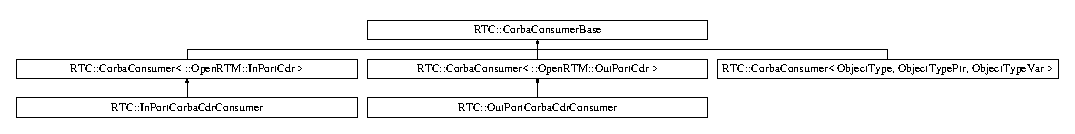
\includegraphics[height=1.34615cm]{classRTC_1_1CorbaConsumerBase}
\end{center}
\end{figure}
\subsection*{Public Member Functions}
\begin{DoxyCompactItemize}
\item 
{\bf CorbaConsumerBase} ()
\begin{DoxyCompactList}\small\item\em Consructor. \item\end{DoxyCompactList}\item 
{\bf CorbaConsumerBase} (const {\bf CorbaConsumerBase} \&x)
\begin{DoxyCompactList}\small\item\em Copy Consructor. \item\end{DoxyCompactList}\item 
{\bf CorbaConsumerBase} \& {\bf operator=} (const {\bf CorbaConsumerBase} \&x)
\begin{DoxyCompactList}\small\item\em Assignment operator. \item\end{DoxyCompactList}\item 
void {\bf swap} ({\bf CorbaConsumerBase} \&x)
\begin{DoxyCompactList}\small\item\em swap function \item\end{DoxyCompactList}\item 
virtual {\bf $\sim$CorbaConsumerBase} (void)
\begin{DoxyCompactList}\small\item\em Virtual destructor. \item\end{DoxyCompactList}\item 
virtual bool {\bf setObject} (CORBA::Object\_\-ptr obj)
\begin{DoxyCompactList}\small\item\em Set CORBA Object. \item\end{DoxyCompactList}\item 
virtual CORBA::Object\_\-ptr {\bf getObject} ()
\begin{DoxyCompactList}\small\item\em Get CORBA Object. \item\end{DoxyCompactList}\item 
virtual void {\bf releaseObject} ()
\begin{DoxyCompactList}\small\item\em Clear CORBA object setting. \item\end{DoxyCompactList}\end{DoxyCompactItemize}
\subsection*{Protected Attributes}
\begin{DoxyCompactItemize}
\item 
CORBA::Object\_\-var {\bf m\_\-objref}
\begin{DoxyCompactList}\small\item\em CORBA object which is set. \item\end{DoxyCompactList}\end{DoxyCompactItemize}


\subsection{Constructor \& Destructor Documentation}
\index{RTC::CorbaConsumerBase@{RTC::CorbaConsumerBase}!CorbaConsumerBase@{CorbaConsumerBase}}
\index{CorbaConsumerBase@{CorbaConsumerBase}!RTC::CorbaConsumerBase@{RTC::CorbaConsumerBase}}
\subsubsection[{CorbaConsumerBase}]{\setlength{\rightskip}{0pt plus 5cm}RTC::CorbaConsumerBase::CorbaConsumerBase ()\hspace{0.3cm}{\ttfamily  [inline]}}\label{classRTC_1_1CorbaConsumerBase_a95aebe603aca268718c13e37f1700603}


Consructor. 

\index{RTC::CorbaConsumerBase@{RTC::CorbaConsumerBase}!CorbaConsumerBase@{CorbaConsumerBase}}
\index{CorbaConsumerBase@{CorbaConsumerBase}!RTC::CorbaConsumerBase@{RTC::CorbaConsumerBase}}
\subsubsection[{CorbaConsumerBase}]{\setlength{\rightskip}{0pt plus 5cm}RTC::CorbaConsumerBase::CorbaConsumerBase (const {\bf CorbaConsumerBase} \& {\em x})\hspace{0.3cm}{\ttfamily  [inline]}}\label{classRTC_1_1CorbaConsumerBase_a0cef39f613583313f8b335259b78cdd2}


Copy Consructor. 


\begin{DoxyParams}{Parameters}
\item[{\em x}]A \doxyref{CorbaConsumerBase}{p.}{classRTC_1_1CorbaConsumerBase} object of copy source \end{DoxyParams}
\index{RTC::CorbaConsumerBase@{RTC::CorbaConsumerBase}!$\sim$CorbaConsumerBase@{$\sim$CorbaConsumerBase}}
\index{$\sim$CorbaConsumerBase@{$\sim$CorbaConsumerBase}!RTC::CorbaConsumerBase@{RTC::CorbaConsumerBase}}
\subsubsection[{$\sim$CorbaConsumerBase}]{\setlength{\rightskip}{0pt plus 5cm}virtual RTC::CorbaConsumerBase::$\sim$CorbaConsumerBase (void)\hspace{0.3cm}{\ttfamily  [inline, virtual]}}\label{classRTC_1_1CorbaConsumerBase_aa6b7667e37b137f3af8c6668da48f01d}


Virtual destructor. 



References releaseObject().



\subsection{Member Function Documentation}
\index{RTC::CorbaConsumerBase@{RTC::CorbaConsumerBase}!getObject@{getObject}}
\index{getObject@{getObject}!RTC::CorbaConsumerBase@{RTC::CorbaConsumerBase}}
\subsubsection[{getObject}]{\setlength{\rightskip}{0pt plus 5cm}virtual CORBA::Object\_\-ptr RTC::CorbaConsumerBase::getObject ()\hspace{0.3cm}{\ttfamily  [inline, virtual]}}\label{classRTC_1_1CorbaConsumerBase_af1d1c9413bf9f017c4bc605ca3a08bd3}


Get CORBA Object. 

Get the object reference held as CORBA::Object\_\-var type in \doxyref{ConsumerBase}{p.}{classConsumerBase} object.

\begin{DoxyReturn}{Returns}
Object reference of CORBA object 
\end{DoxyReturn}


References m\_\-objref.

\index{RTC::CorbaConsumerBase@{RTC::CorbaConsumerBase}!operator=@{operator=}}
\index{operator=@{operator=}!RTC::CorbaConsumerBase@{RTC::CorbaConsumerBase}}
\subsubsection[{operator=}]{\setlength{\rightskip}{0pt plus 5cm}{\bf CorbaConsumerBase}\& RTC::CorbaConsumerBase::operator= (const {\bf CorbaConsumerBase} \& {\em x})\hspace{0.3cm}{\ttfamily  [inline]}}\label{classRTC_1_1CorbaConsumerBase_af070cffba7981a1c42b7be15b01c8543}


Assignment operator. 


\begin{DoxyParams}{Parameters}
\item[{\em x}]Copy source.\end{DoxyParams}
\begin{DoxyReturn}{Returns}
An assignment result 
\end{DoxyReturn}


References swap().

\index{RTC::CorbaConsumerBase@{RTC::CorbaConsumerBase}!releaseObject@{releaseObject}}
\index{releaseObject@{releaseObject}!RTC::CorbaConsumerBase@{RTC::CorbaConsumerBase}}
\subsubsection[{releaseObject}]{\setlength{\rightskip}{0pt plus 5cm}virtual void RTC::CorbaConsumerBase::releaseObject ()\hspace{0.3cm}{\ttfamily  [inline, virtual]}}\label{classRTC_1_1CorbaConsumerBase_aafdaaab4a66319fe5ab1486b1001dfb9}


Clear CORBA object setting. 

Clear CORBA object which is set. Operate nothing for CORBA object itself. 

Reimplemented in {\bf RTC::CorbaConsumer$<$ ObjectType, ObjectTypePtr, ObjectTypeVar $>$} \doxyref{}{p.}{classRTC_1_1CorbaConsumer_aaebca7bff42ba840684cf51fb8577290}, {\bf RTC::CorbaConsumer$<$ ::OpenRTM::InPortCdr $>$} \doxyref{}{p.}{classRTC_1_1CorbaConsumer_aaebca7bff42ba840684cf51fb8577290}, and {\bf RTC::CorbaConsumer$<$ ::OpenRTM::OutPortCdr $>$} \doxyref{}{p.}{classRTC_1_1CorbaConsumer_aaebca7bff42ba840684cf51fb8577290}.



References m\_\-objref.



Referenced by $\sim$CorbaConsumerBase().

\index{RTC::CorbaConsumerBase@{RTC::CorbaConsumerBase}!setObject@{setObject}}
\index{setObject@{setObject}!RTC::CorbaConsumerBase@{RTC::CorbaConsumerBase}}
\subsubsection[{setObject}]{\setlength{\rightskip}{0pt plus 5cm}virtual bool RTC::CorbaConsumerBase::setObject (CORBA::Object\_\-ptr {\em obj})\hspace{0.3cm}{\ttfamily  [inline, virtual]}}\label{classRTC_1_1CorbaConsumerBase_aa91cc706b62c6782f79bfc76663f3dcc}


Set CORBA Object. 

The given CORBA Object is held as CORBA::Object\_\-var type in \doxyref{ConsumerBase}{p.}{classConsumerBase} object.


\begin{DoxyParams}{Parameters}
\item[{\em obj}]Object reference of CORBA object\end{DoxyParams}
\begin{DoxyReturn}{Returns}
If obj is nil reference, it returns false. 
\end{DoxyReturn}


Reimplemented in {\bf RTC::CorbaConsumer$<$ ObjectType, ObjectTypePtr, ObjectTypeVar $>$} \doxyref{}{p.}{classRTC_1_1CorbaConsumer_a8e5db22a71b01b1a8178d9966eb6499d}, {\bf RTC::CorbaConsumer$<$ ::OpenRTM::InPortCdr $>$} \doxyref{}{p.}{classRTC_1_1CorbaConsumer_a8e5db22a71b01b1a8178d9966eb6499d}, and {\bf RTC::CorbaConsumer$<$ ::OpenRTM::OutPortCdr $>$} \doxyref{}{p.}{classRTC_1_1CorbaConsumer_a8e5db22a71b01b1a8178d9966eb6499d}.



References m\_\-objref.



Referenced by RTC::CorbaConsumer$<$ ::OpenRTM::OutPortCdr $>$::setObject().

\index{RTC::CorbaConsumerBase@{RTC::CorbaConsumerBase}!swap@{swap}}
\index{swap@{swap}!RTC::CorbaConsumerBase@{RTC::CorbaConsumerBase}}
\subsubsection[{swap}]{\setlength{\rightskip}{0pt plus 5cm}void RTC::CorbaConsumerBase::swap ({\bf CorbaConsumerBase} \& {\em x})\hspace{0.3cm}{\ttfamily  [inline]}}\label{classRTC_1_1CorbaConsumerBase_a7dd51f4e04ab755dcd7d5e01fd6aca2f}


swap function 


\begin{DoxyParams}{Parameters}
\item[{\em x}]Copy source. \end{DoxyParams}


References m\_\-objref.



Referenced by operator=().



\subsection{Member Data Documentation}
\index{RTC::CorbaConsumerBase@{RTC::CorbaConsumerBase}!m\_\-objref@{m\_\-objref}}
\index{m\_\-objref@{m\_\-objref}!RTC::CorbaConsumerBase@{RTC::CorbaConsumerBase}}
\subsubsection[{m\_\-objref}]{\setlength{\rightskip}{0pt plus 5cm}CORBA::Object\_\-var {\bf RTC::CorbaConsumerBase::m\_\-objref}\hspace{0.3cm}{\ttfamily  [protected]}}\label{classRTC_1_1CorbaConsumerBase_a08aa594ab325d7ee84fecba104c41478}


CORBA object which is set. 



Referenced by getObject(), releaseObject(), RTC::CorbaConsumer$<$ ::OpenRTM::OutPortCdr $>$::setObject(), setObject(), and swap().


\section{RTC::CorbaNaming Class Reference}
\label{classRTC_1_1CorbaNaming}\index{RTC::CorbaNaming@{RTC::CorbaNaming}}


CORBA Naming Service helper class.  




{\ttfamily \#include $<$CorbaNaming.h$>$}

\subsection*{Public Types}
\begin{DoxyCompactItemize}
\item 
typedef CORBA::SystemException {\bf SystemException}
\item 
typedef CosNaming::NamingContext::NotFound {\bf NotFound}
\item 
typedef CosNaming::NamingContext::CannotProceed {\bf CannotProceed}
\item 
typedef CosNaming::NamingContext::InvalidName {\bf InvalidName}
\item 
typedef CosNaming::NamingContext::AlreadyBound {\bf AlreadyBound}
\item 
typedef CosNaming::NamingContext::NotEmpty {\bf NotEmpty}
\item 
typedef CosNaming::NamingContextExt::InvalidAddress {\bf InvalidAddress}
\item 
typedef std::vector$<$ CORBA::Object\_\-ptr $>$ {\bf ObjectList}
\end{DoxyCompactItemize}
\subsection*{Public Member Functions}
\begin{DoxyCompactItemize}
\item 
{\bf CorbaNaming} (CORBA::ORB\_\-ptr orb)
\begin{DoxyCompactList}\small\item\em Consructor. \item\end{DoxyCompactList}\item 
{\bf CorbaNaming} (CORBA::ORB\_\-ptr orb, const char $\ast$name\_\-server)
\begin{DoxyCompactList}\small\item\em Consructor. \item\end{DoxyCompactList}\item 
virtual {\bf $\sim$CorbaNaming} (void)
\begin{DoxyCompactList}\small\item\em Virtual destructor. \item\end{DoxyCompactList}\item 
void {\bf init} (const char $\ast$name\_\-server)
\begin{DoxyCompactList}\small\item\em Initialize the Naming Service. \item\end{DoxyCompactList}\item 
bool {\bf isAlive} ()
\item 
void {\bf bind} (const CosNaming::Name \&name, CORBA::Object\_\-ptr obj, const bool force=1)  throw (SystemException, NotFound, CannotProceed,             InvalidName, AlreadyBound)
\begin{DoxyCompactList}\small\item\em Bind object on specified name component position. \item\end{DoxyCompactList}\item 
void {\bf bindByString} (const char $\ast$string\_\-name, CORBA::Object\_\-ptr obj, const bool force=1)  throw (SystemException, NotFound, CannotProceed,             InvalidName, AlreadyBound)
\begin{DoxyCompactList}\small\item\em Bind object on specified string name position. \item\end{DoxyCompactList}\item 
void {\bf bindRecursive} (CosNaming::NamingContext\_\-ptr context, const CosNaming::Name \&name, CORBA::Object\_\-ptr obj)  throw (SystemException, CannotProceed, InvalidName, AlreadyBound)
\begin{DoxyCompactList}\small\item\em Bind intermediate context recursively and bind object. \item\end{DoxyCompactList}\item 
void {\bf rebind} (const CosNaming::Name \&name, CORBA::Object\_\-ptr obj, const bool force=1)  throw (SystemException, NotFound, CannotProceed, InvalidName)
\begin{DoxyCompactList}\small\item\em Rebind object. \item\end{DoxyCompactList}\item 
void {\bf rebindByString} (const char $\ast$string\_\-name, CORBA::Object\_\-ptr obj, const bool force=1)  throw (SystemException, NotFound, CannotProceed, InvalidName)
\begin{DoxyCompactList}\small\item\em Rebind Object. \item\end{DoxyCompactList}\item 
void {\bf rebindRecursive} (CosNaming::NamingContext\_\-ptr context, const CosNaming::Name \&name, CORBA::Object\_\-ptr obj)  throw (SystemException, CannotProceed, InvalidName)
\begin{DoxyCompactList}\small\item\em Bind intermediate context recursively and rebind object. \item\end{DoxyCompactList}\item 
void {\bf bindContext} (const CosNaming::Name \&name, CosNaming::NamingContext\_\-ptr name\_\-cxt, const bool force=1)  throw (SystemException, NotFound, CannotProceed,             InvalidName, AlreadyBound)
\begin{DoxyCompactList}\small\item\em Bind NamingContext. \item\end{DoxyCompactList}\item 
void {\bf bindContext} (const char $\ast$string\_\-name, CosNaming::NamingContext\_\-ptr name\_\-cxt, const bool force=1)  throw (SystemException, NotFound, CannotProceed,             InvalidName, AlreadyBound)
\begin{DoxyCompactList}\small\item\em Bind NamingContext. \item\end{DoxyCompactList}\item 
void {\bf bindContextRecursive} (CosNaming::NamingContext\_\-ptr context, const CosNaming::Name \&name, CosNaming::NamingContext\_\-ptr name\_\-cxt)
\begin{DoxyCompactList}\small\item\em Bind intermediate context recursively and bind NamingContext. \item\end{DoxyCompactList}\item 
void {\bf rebindContext} (const CosNaming::Name \&name, CosNaming::NamingContext\_\-ptr name\_\-cxt, const bool force=1)  throw (SystemException, NotFound, CannotProceed, InvalidName)
\begin{DoxyCompactList}\small\item\em Rebind NamingContext. \item\end{DoxyCompactList}\item 
void {\bf rebindContext} (const char $\ast$string\_\-name, CosNaming::NamingContext\_\-ptr name\_\-cxt, const bool force=1)  throw (SystemException, NotFound, CannotProceed, InvalidName)
\begin{DoxyCompactList}\small\item\em Rebind NamingContext. \item\end{DoxyCompactList}\item 
void {\bf rebindContextRecursive} (CosNaming::NamingContext\_\-ptr context, const CosNaming::Name \&name, CosNaming::NamingContext\_\-ptr name\_\-cxt)
\begin{DoxyCompactList}\small\item\em Rebind intermediate context recursively and rebind NamingContext. \item\end{DoxyCompactList}\item 
CORBA::Object\_\-ptr {\bf resolve} (const CosNaming::Name \&name)  throw (SystemException, NotFound, CannotProceed, InvalidName)
\begin{DoxyCompactList}\small\item\em Return object bound on the specified NameComponent. \item\end{DoxyCompactList}\item 
CORBA::Object\_\-ptr {\bf resolve} (const char $\ast$string\_\-name)  throw (SystemException, NotFound, CannotProceed, InvalidName)
\begin{DoxyCompactList}\small\item\em Return object bound on the specified name. \item\end{DoxyCompactList}\item 
void {\bf unbind} (const CosNaming::Name \&name)  throw (SystemException, NotFound, CannotProceed, InvalidName)
\begin{DoxyCompactList}\small\item\em Unbind a binding specified by NameComponent. \item\end{DoxyCompactList}\item 
void {\bf unbind} (const char $\ast$string\_\-name)  throw (SystemException, NotFound, CannotProceed, InvalidName)
\begin{DoxyCompactList}\small\item\em Unbind a binding specified by string representation. \item\end{DoxyCompactList}\item 
CosNaming::NamingContext\_\-ptr {\bf newContext} ()
\begin{DoxyCompactList}\small\item\em Create new NamingContext. \item\end{DoxyCompactList}\item 
CosNaming::NamingContext\_\-ptr {\bf bindNewContext} (const CosNaming::Name \&name, bool force=true)  throw (SystemException, NotFound, CannotProceed,             InvalidName, AlreadyBound)
\begin{DoxyCompactList}\small\item\em Bind new NamingContext. \item\end{DoxyCompactList}\item 
CosNaming::NamingContext\_\-ptr {\bf bindNewContext} (const char $\ast$string\_\-name, bool force=true)  throw (SystemException, NotFound, CannotProceed,             InvalidName, AlreadyBound)
\begin{DoxyCompactList}\small\item\em Bind new NamingContext. \item\end{DoxyCompactList}\item 
void {\bf destroy} (CosNaming::NamingContext\_\-ptr context)  throw (SystemException, NotEmpty)
\begin{DoxyCompactList}\small\item\em Destroy the naming context. \item\end{DoxyCompactList}\item 
void {\bf destroyRecursive} (CosNaming::NamingContext\_\-ptr context)  throw (SystemException, NotEmpty, NotFound, CannotProceed, InvalidName)
\begin{DoxyCompactList}\small\item\em Destroy the naming context recursively. \item\end{DoxyCompactList}\item 
void {\bf clearAll} ()
\begin{DoxyCompactList}\small\item\em Destroy all bindings. \item\end{DoxyCompactList}\item 
void {\bf list} (CosNaming::NamingContext\_\-ptr name\_\-cxt, CORBA::ULong how\_\-many, CosNaming::BindingList\_\-var \&bl, CosNaming::BindingIterator\_\-var \&bi)
\begin{DoxyCompactList}\small\item\em Get Binding of the given NamingContext. \item\end{DoxyCompactList}\item 
char $\ast$ {\bf toString} (const CosNaming::Name \&name)  throw (SystemException, InvalidName)
\begin{DoxyCompactList}\small\item\em Get string representation of given NameComponent. \item\end{DoxyCompactList}\item 
CosNaming::Name {\bf toName} (const char $\ast$string\_\-name)  throw (SystemException, InvalidName)
\begin{DoxyCompactList}\small\item\em Resolve given string representation to NameComponent. \item\end{DoxyCompactList}\item 
char $\ast$ {\bf toUrl} (char $\ast$addr, char $\ast$string\_\-name)  throw (SystemException, InvalidAddress, InvalidName)
\begin{DoxyCompactList}\small\item\em Get URL representation from given addr and string\_\-name. \item\end{DoxyCompactList}\item 
CORBA::Object\_\-ptr {\bf resolveStr} (const char $\ast$string\_\-name)  throw (SystemException, NotFound, CannotProceed,             InvalidName, AlreadyBound)
\begin{DoxyCompactList}\small\item\em Resolve from name of string representation and get object. \item\end{DoxyCompactList}\item 
CORBA::Object\_\-ptr {\bf bindOrResolve} (CosNaming::NamingContext\_\-ptr context, const CosNaming::Name \&name, CORBA::Object\_\-ptr obj)
\begin{DoxyCompactList}\small\item\em Bind or resolve the given name component. \item\end{DoxyCompactList}\item 
CosNaming::NamingContext\_\-ptr {\bf bindOrResolveContext} (CosNaming::NamingContext\_\-ptr context, const CosNaming::Name \&name, CosNaming::NamingContext\_\-ptr new\_\-context)
\begin{DoxyCompactList}\small\item\em Bind or resolve the given name component. \item\end{DoxyCompactList}\item 
CosNaming::NamingContext\_\-ptr {\bf bindOrResolveContext} (CosNaming::NamingContext\_\-ptr context, const CosNaming::Name \&name)
\begin{DoxyCompactList}\small\item\em Bind or resolve the given name component. \item\end{DoxyCompactList}\item 
const char $\ast$ {\bf getNameServer} ()
\begin{DoxyCompactList}\small\item\em Get the name of name server. \item\end{DoxyCompactList}\item 
CosNaming::NamingContext\_\-ptr {\bf getRootContext} ()
\begin{DoxyCompactList}\small\item\em Get the root context. \item\end{DoxyCompactList}\item 
bool {\bf isNamingContext} (CORBA::Object\_\-ptr obj)
\begin{DoxyCompactList}\small\item\em Determine whether the object is NamingContext. \item\end{DoxyCompactList}\item 
bool {\bf isNamingContext} (const CosNaming::Name \&name)
\begin{DoxyCompactList}\small\item\em Determine whether the given name component is NamingContext. \item\end{DoxyCompactList}\item 
bool {\bf isNamingContext} (const char $\ast$string\_\-name)
\begin{DoxyCompactList}\small\item\em Determine whether the given string name is NamingContext. \item\end{DoxyCompactList}\item 
CosNaming::Name {\bf subName} (const CosNaming::Name \&name, CORBA::Long begin, CORBA::Long end=-\/1)
\begin{DoxyCompactList}\small\item\em Get subset of given name component. \item\end{DoxyCompactList}\end{DoxyCompactItemize}
\subsection*{Protected Member Functions}
\begin{DoxyCompactItemize}
\item 
void {\bf nameToString} (const CosNaming::Name \&name, char $\ast$string\_\-name, CORBA::ULong slen)
\begin{DoxyCompactList}\small\item\em Get string representation of name component. \item\end{DoxyCompactList}\item 
CORBA::ULong {\bf getNameLength} (const CosNaming::Name \&name)
\begin{DoxyCompactList}\small\item\em Get string length of the name component's string representation. \item\end{DoxyCompactList}\item 
unsigned int {\bf split} (const std::string \&input, const std::string \&delimiter, std::vector$<$ std::string $>$ \&results)
\begin{DoxyCompactList}\small\item\em Split of string. \item\end{DoxyCompactList}\end{DoxyCompactItemize}
\subsection*{Protected Attributes}
\begin{DoxyCompactItemize}
\item 
CORBA::ORB\_\-var {\bf m\_\-varORB}
\begin{DoxyCompactList}\small\item\em ORB. \item\end{DoxyCompactList}\item 
std::string {\bf m\_\-nameServer}
\begin{DoxyCompactList}\small\item\em Name of the name server. \item\end{DoxyCompactList}\item 
CosNaming::NamingContextExt\_\-var {\bf m\_\-rootContext}
\begin{DoxyCompactList}\small\item\em The root context of specified name server. \item\end{DoxyCompactList}\end{DoxyCompactItemize}


\subsection{Detailed Description}
CORBA Naming Service helper class. This class is a wrapper class of CosNaming::NamingContext. Almost the same operations which CosNaming::NamingContext has are provided, and some operation allows string naming representation of context and object instead of CosNaming::Name.

The object of the class would connect to a CORBA naming server at the instantiation or immediately after instantiation. After that the object invokes operations to the root context of it. This class realizes forced binding to deep NamingContext, without binding intermediate NamingContexts explicitly.

\begin{DoxySince}{Since}
0.4.0 
\end{DoxySince}


\subsection{Member Typedef Documentation}
\index{RTC::CorbaNaming@{RTC::CorbaNaming}!AlreadyBound@{AlreadyBound}}
\index{AlreadyBound@{AlreadyBound}!RTC::CorbaNaming@{RTC::CorbaNaming}}
\subsubsection[{AlreadyBound}]{\setlength{\rightskip}{0pt plus 5cm}typedef CosNaming::NamingContext::AlreadyBound {\bf RTC::CorbaNaming::AlreadyBound}}\label{classRTC_1_1CorbaNaming_a6669a088b188bbf53d96328945db065f}
\index{RTC::CorbaNaming@{RTC::CorbaNaming}!CannotProceed@{CannotProceed}}
\index{CannotProceed@{CannotProceed}!RTC::CorbaNaming@{RTC::CorbaNaming}}
\subsubsection[{CannotProceed}]{\setlength{\rightskip}{0pt plus 5cm}typedef CosNaming::NamingContext::CannotProceed {\bf RTC::CorbaNaming::CannotProceed}}\label{classRTC_1_1CorbaNaming_a77504e9d1028c3f524151edda4c5faf4}
\index{RTC::CorbaNaming@{RTC::CorbaNaming}!InvalidAddress@{InvalidAddress}}
\index{InvalidAddress@{InvalidAddress}!RTC::CorbaNaming@{RTC::CorbaNaming}}
\subsubsection[{InvalidAddress}]{\setlength{\rightskip}{0pt plus 5cm}typedef CosNaming::NamingContextExt::InvalidAddress {\bf RTC::CorbaNaming::InvalidAddress}}\label{classRTC_1_1CorbaNaming_af3580312d8a2e6d00ad3dca75b3cfae3}
\index{RTC::CorbaNaming@{RTC::CorbaNaming}!InvalidName@{InvalidName}}
\index{InvalidName@{InvalidName}!RTC::CorbaNaming@{RTC::CorbaNaming}}
\subsubsection[{InvalidName}]{\setlength{\rightskip}{0pt plus 5cm}typedef CosNaming::NamingContext::InvalidName {\bf RTC::CorbaNaming::InvalidName}}\label{classRTC_1_1CorbaNaming_ab79889ab5d3a28c494ee8768200e3683}
\index{RTC::CorbaNaming@{RTC::CorbaNaming}!NotEmpty@{NotEmpty}}
\index{NotEmpty@{NotEmpty}!RTC::CorbaNaming@{RTC::CorbaNaming}}
\subsubsection[{NotEmpty}]{\setlength{\rightskip}{0pt plus 5cm}typedef CosNaming::NamingContext::NotEmpty {\bf RTC::CorbaNaming::NotEmpty}}\label{classRTC_1_1CorbaNaming_a223ee860ea0ffa395e688b6eb0fd3b11}
\index{RTC::CorbaNaming@{RTC::CorbaNaming}!NotFound@{NotFound}}
\index{NotFound@{NotFound}!RTC::CorbaNaming@{RTC::CorbaNaming}}
\subsubsection[{NotFound}]{\setlength{\rightskip}{0pt plus 5cm}typedef CosNaming::NamingContext::NotFound {\bf RTC::CorbaNaming::NotFound}}\label{classRTC_1_1CorbaNaming_a92e7f10507946507a4e8daf126ecc409}
\index{RTC::CorbaNaming@{RTC::CorbaNaming}!ObjectList@{ObjectList}}
\index{ObjectList@{ObjectList}!RTC::CorbaNaming@{RTC::CorbaNaming}}
\subsubsection[{ObjectList}]{\setlength{\rightskip}{0pt plus 5cm}typedef std::vector$<$CORBA::Object\_\-ptr$>$ {\bf RTC::CorbaNaming::ObjectList}}\label{classRTC_1_1CorbaNaming_aea8dfd52409e620da87cc1b1a7e835cc}
\index{RTC::CorbaNaming@{RTC::CorbaNaming}!SystemException@{SystemException}}
\index{SystemException@{SystemException}!RTC::CorbaNaming@{RTC::CorbaNaming}}
\subsubsection[{SystemException}]{\setlength{\rightskip}{0pt plus 5cm}typedef CORBA::SystemException {\bf RTC::CorbaNaming::SystemException}}\label{classRTC_1_1CorbaNaming_adcd493bdbf96b312ce1b985b8a08c79d}


\subsection{Constructor \& Destructor Documentation}
\index{RTC::CorbaNaming@{RTC::CorbaNaming}!CorbaNaming@{CorbaNaming}}
\index{CorbaNaming@{CorbaNaming}!RTC::CorbaNaming@{RTC::CorbaNaming}}
\subsubsection[{CorbaNaming}]{\setlength{\rightskip}{0pt plus 5cm}RTC::CorbaNaming::CorbaNaming (CORBA::ORB\_\-ptr {\em orb})}\label{classRTC_1_1CorbaNaming_a081d0658c45831f74dcefb3b2bccb631}


Consructor. 


\begin{DoxyParams}{Parameters}
\item[{\em orb}]ORB \end{DoxyParams}
\index{RTC::CorbaNaming@{RTC::CorbaNaming}!CorbaNaming@{CorbaNaming}}
\index{CorbaNaming@{CorbaNaming}!RTC::CorbaNaming@{RTC::CorbaNaming}}
\subsubsection[{CorbaNaming}]{\setlength{\rightskip}{0pt plus 5cm}RTC::CorbaNaming::CorbaNaming (CORBA::ORB\_\-ptr {\em orb}, \/  const char $\ast$ {\em name\_\-server})}\label{classRTC_1_1CorbaNaming_ae9e84d1814b4664789d2d1d88f13f97f}


Consructor. 


\begin{DoxyParams}{Parameters}
\item[{\em orb}]ORB \item[{\em name\_\-server}]Name of the name server \end{DoxyParams}
\index{RTC::CorbaNaming@{RTC::CorbaNaming}!$\sim$CorbaNaming@{$\sim$CorbaNaming}}
\index{$\sim$CorbaNaming@{$\sim$CorbaNaming}!RTC::CorbaNaming@{RTC::CorbaNaming}}
\subsubsection[{$\sim$CorbaNaming}]{\setlength{\rightskip}{0pt plus 5cm}virtual RTC::CorbaNaming::$\sim$CorbaNaming (void)\hspace{0.3cm}{\ttfamily  [inline, virtual]}}\label{classRTC_1_1CorbaNaming_ad929fafaa24f3360341aeb1a4e8ee826}


Virtual destructor. 



\subsection{Member Function Documentation}
\index{RTC::CorbaNaming@{RTC::CorbaNaming}!bind@{bind}}
\index{bind@{bind}!RTC::CorbaNaming@{RTC::CorbaNaming}}
\subsubsection[{bind}]{\setlength{\rightskip}{0pt plus 5cm}void RTC::CorbaNaming::bind (const CosNaming::Name \& {\em name}, \/  CORBA::Object\_\-ptr {\em obj}, \/  const bool {\em force} = {\ttfamily 1})  throw ({\bf SystemException}, {\bf NotFound}, {\bf CannotProceed},             {\bf InvalidName}, {\bf AlreadyBound})}\label{classRTC_1_1CorbaNaming_ac21620f79aecc1bf989629b7aac2938f}


Bind object on specified name component position. 

Almost the same operation as CosNaming::bind(), but there is a difference that \doxyref{bind()}{p.}{classRTC_1_1CorbaNaming_ac21620f79aecc1bf989629b7aac2938f} is invoked for the root context of the given name server.

Bind between Name $<$name$>$ and Object $<$obj$>$ on this NamingContext. If c\_\-n indicates the n-\/th of NameComponent, when name consists of n pieces of NameComponent, it is handled as follows.

cxt-\/$>$bind($<$c\_\-1, c\_\-2, ... c\_\-n$>$, obj) is the same as the following operation. cxt-\/$>$resolve($<$c\_\-1, ... c\_\-(n-\/1)$>$)-\/$>$bind($<$c\_\-n$>$, obj)

In other word, resolve from the first to the (n-\/1)th context and bind obj as name$<$n$>$ on the (n-\/1)th context. NemingContext of $<$c\_\-1, ... c\_\-(n-\/1)$>$ for resolving name must be already bound in \doxyref{bindContext()}{p.}{classRTC_1_1CorbaNaming_a1eaa278d91546b514fdf361a0bfcbf87} or \doxyref{rebindContext()}{p.}{classRTC_1_1CorbaNaming_afd9649388ba4f49b53d036b50e311df0}. If NamingContext of $<$c\_\-1, ... c\_\-(n-\/1)$>$ does not exist, NotFound excption will occur.

However, when flag of forced bind is true, even if $<$c\_\-1, ... c\_\-(n-\/1)$>$ does not exist, finally obj will be bound to name name $<$c\_\-n$>$ by binding to the context recursively.

Even in any case, if the object of name$<$n$>$ (Object or context) is bound on the (n-\/1)th context, AlreadyBound exception will occur.


\begin{DoxyParams}{Parameters}
\item[{\em name}]NameComponent of name applied to object \item[{\em obj}]Object that is associated \item[{\em force}]If true, the intermediate context is bound forcibly. (The default value:true)\end{DoxyParams}

\begin{DoxyExceptions}{Exceptions}
\item[{\em NotFound}]There is not $<$c\_\-1, c\_\-2, ..., c\_\-(n-\/1)$>$. \item[{\em CannotProceed}]Processing cannot be continued for some reasons. \item[{\em InvalidName}]The argument 'name' is invalid. \item[{\em AlreadyBound}]The object of name$<$c\_\-n$>$ is already bound. \end{DoxyExceptions}
\index{RTC::CorbaNaming@{RTC::CorbaNaming}!bindByString@{bindByString}}
\index{bindByString@{bindByString}!RTC::CorbaNaming@{RTC::CorbaNaming}}
\subsubsection[{bindByString}]{\setlength{\rightskip}{0pt plus 5cm}void RTC::CorbaNaming::bindByString (const char $\ast$ {\em string\_\-name}, \/  CORBA::Object\_\-ptr {\em obj}, \/  const bool {\em force} = {\ttfamily 1})  throw ({\bf SystemException}, {\bf NotFound}, {\bf CannotProceed},             {\bf InvalidName}, {\bf AlreadyBound})}\label{classRTC_1_1CorbaNaming_a88fba8eb04bf1a2b631007d0d87ea28f}


Bind object on specified string name position. 

This is the same as \doxyref{bind()}{p.}{classRTC_1_1CorbaNaming_ac21620f79aecc1bf989629b7aac2938f} except as the given name is string representation when Object is bound. bind(toName(string\_\-name),obj) is the same.


\begin{DoxyParams}{Parameters}
\item[{\em string\_\-name}]The string representation of name applied to object \item[{\em obj}]Object that is associated \item[{\em force}]If true, the intermediate context is bound forcibly. (The default value:true)\end{DoxyParams}

\begin{DoxyExceptions}{Exceptions}
\item[{\em NotFound}]There is not $<$c\_\-1, c\_\-2, ..., c\_\-(n-\/1)$>$. \item[{\em CannotProceed}]Processing cannot be continued for some reasons. \item[{\em InvalidName}]The argument 'name' is invalid. \item[{\em AlreadyBound}]The object of name$<$c\_\-n$>$ is already bound. \end{DoxyExceptions}
\index{RTC::CorbaNaming@{RTC::CorbaNaming}!bindContext@{bindContext}}
\index{bindContext@{bindContext}!RTC::CorbaNaming@{RTC::CorbaNaming}}
\subsubsection[{bindContext}]{\setlength{\rightskip}{0pt plus 5cm}void RTC::CorbaNaming::bindContext (const char $\ast$ {\em string\_\-name}, \/  CosNaming::NamingContext\_\-ptr {\em name\_\-cxt}, \/  const bool {\em force} = {\ttfamily 1})  throw ({\bf SystemException}, {\bf NotFound}, {\bf CannotProceed},             {\bf InvalidName}, {\bf AlreadyBound})}\label{classRTC_1_1CorbaNaming_a62c211af81e61ccc9dcbbf8c0f26eb15}


Bind NamingContext. 

This is the same as \doxyref{bindByString()}{p.}{classRTC_1_1CorbaNaming_a88fba8eb04bf1a2b631007d0d87ea28f} except as the bound object is NamingContext.


\begin{DoxyParams}{Parameters}
\item[{\em string\_\-name}]String representation of name applied to object \item[{\em name\_\-cxt}]NamingContext that is associated \item[{\em force}]If true, the intermediate context is bound forcibly. (The default value:true)\end{DoxyParams}

\begin{DoxyExceptions}{Exceptions}
\item[{\em NotFound}]There is not $<$c\_\-1, c\_\-2, ..., c\_\-(n-\/1)$>$. \item[{\em CannotProceed}]Processing cannot be continued for some reasons. \item[{\em InvalidName}]The argument 'name' is invalid. \item[{\em AlreadyBound}]The object of name$<$n$>$ is already bound. \end{DoxyExceptions}
\index{RTC::CorbaNaming@{RTC::CorbaNaming}!bindContext@{bindContext}}
\index{bindContext@{bindContext}!RTC::CorbaNaming@{RTC::CorbaNaming}}
\subsubsection[{bindContext}]{\setlength{\rightskip}{0pt plus 5cm}void RTC::CorbaNaming::bindContext (const CosNaming::Name \& {\em name}, \/  CosNaming::NamingContext\_\-ptr {\em name\_\-cxt}, \/  const bool {\em force} = {\ttfamily 1})  throw ({\bf SystemException}, {\bf NotFound}, {\bf CannotProceed},             {\bf InvalidName}, {\bf AlreadyBound})}\label{classRTC_1_1CorbaNaming_a1eaa278d91546b514fdf361a0bfcbf87}


Bind NamingContext. 

This is the same as \doxyref{bind()}{p.}{classRTC_1_1CorbaNaming_ac21620f79aecc1bf989629b7aac2938f} except as the bound object is NamingContext.


\begin{DoxyParams}{Parameters}
\item[{\em name}]NameComponent of name applied to object \item[{\em name\_\-cxt}]Object that is associated \item[{\em force}]If true, the intermediate context is bound forcibly. (The default value:true)\end{DoxyParams}

\begin{DoxyExceptions}{Exceptions}
\item[{\em NotFound}]There is not $<$c\_\-1, c\_\-2, ..., c\_\-(n-\/1)$>$. \item[{\em CannotProceed}]Processing cannot be continued for some reasons. \item[{\em InvalidName}]The argument 'name' is invalid. \item[{\em AlreadyBound}]The object of name$<$c\_\-n$>$ is already bound. \end{DoxyExceptions}
\index{RTC::CorbaNaming@{RTC::CorbaNaming}!bindContextRecursive@{bindContextRecursive}}
\index{bindContextRecursive@{bindContextRecursive}!RTC::CorbaNaming@{RTC::CorbaNaming}}
\subsubsection[{bindContextRecursive}]{\setlength{\rightskip}{0pt plus 5cm}void RTC::CorbaNaming::bindContextRecursive (CosNaming::NamingContext\_\-ptr {\em context}, \/  const CosNaming::Name \& {\em name}, \/  CosNaming::NamingContext\_\-ptr {\em name\_\-cxt})}\label{classRTC_1_1CorbaNaming_acefcc23ad029cbf3d989ffc61adc4d35}


Bind intermediate context recursively and bind NamingContext. 

This is the same as \doxyref{bindRecursive()}{p.}{classRTC_1_1CorbaNaming_a5417cf439f8efd84f9d13d212f9e62bd} except as the bound object is NamingContext.


\begin{DoxyParams}{Parameters}
\item[{\em context}]NamingContext that starts the bind \item[{\em name}]NameComponent of name applied to object \item[{\em name\_\-cxt}]NamingContext that is associated \end{DoxyParams}
\index{RTC::CorbaNaming@{RTC::CorbaNaming}!bindNewContext@{bindNewContext}}
\index{bindNewContext@{bindNewContext}!RTC::CorbaNaming@{RTC::CorbaNaming}}
\subsubsection[{bindNewContext}]{\setlength{\rightskip}{0pt plus 5cm}CosNaming::NamingContext\_\-ptr RTC::CorbaNaming::bindNewContext (const char $\ast$ {\em string\_\-name}, \/  bool {\em force} = {\ttfamily true})  throw ({\bf SystemException}, {\bf NotFound}, {\bf CannotProceed},             {\bf InvalidName}, {\bf AlreadyBound})}\label{classRTC_1_1CorbaNaming_a7736c378704e3395532b3e05075121f5}


Bind new NamingContext. 

Bind new context corresponding to the given string. The created NamingContext is a creation on the name server.


\begin{DoxyParams}{Parameters}
\item[{\em string\_\-name}]The string representation of name applied to NamingContext \item[{\em force}]If true, the intermediate context is bound forcibly. (The default value:true)\end{DoxyParams}
\begin{DoxyReturn}{Returns}
New created NamingContext
\end{DoxyReturn}

\begin{DoxyExceptions}{Exceptions}
\item[{\em NotFound}]There is not $<$c\_\-1, c\_\-2, ..., c\_\-(n-\/1)$>$. \item[{\em CannotProceed}]Processing cannot be continued for some reasons. \item[{\em InvalidName}]The argument 'name' is invalid. \item[{\em AlreadyBound}]The object of name$<$n$>$ is already bound. \end{DoxyExceptions}
\index{RTC::CorbaNaming@{RTC::CorbaNaming}!bindNewContext@{bindNewContext}}
\index{bindNewContext@{bindNewContext}!RTC::CorbaNaming@{RTC::CorbaNaming}}
\subsubsection[{bindNewContext}]{\setlength{\rightskip}{0pt plus 5cm}CosNaming::NamingContext\_\-ptr RTC::CorbaNaming::bindNewContext (const CosNaming::Name \& {\em name}, \/  bool {\em force} = {\ttfamily true})  throw ({\bf SystemException}, {\bf NotFound}, {\bf CannotProceed},             {\bf InvalidName}, {\bf AlreadyBound})}\label{classRTC_1_1CorbaNaming_a7a1bd265833e6e101ea03926f5e30c52}


Bind new NamingContext. 

Bind new context for the given name. The created NamingContext is a creation on the name server.


\begin{DoxyParams}{Parameters}
\item[{\em name}]NameComponent applied to NamingContext \item[{\em force}]If true, the intermediate context is bound forcibly. (The default value:true)\end{DoxyParams}
\begin{DoxyReturn}{Returns}
New created NamingContext
\end{DoxyReturn}

\begin{DoxyExceptions}{Exceptions}
\item[{\em NotFound}]There is not $<$c\_\-1, c\_\-2, ..., c\_\-(n-\/1)$>$. \item[{\em CannotProceed}]Processing cannot be continued for some reasons. \item[{\em InvalidName}]The argument 'name' is invalid. \item[{\em AlreadyBound}]The object of name$<$n$>$ is already bound. \end{DoxyExceptions}
\index{RTC::CorbaNaming@{RTC::CorbaNaming}!bindOrResolve@{bindOrResolve}}
\index{bindOrResolve@{bindOrResolve}!RTC::CorbaNaming@{RTC::CorbaNaming}}
\subsubsection[{bindOrResolve}]{\setlength{\rightskip}{0pt plus 5cm}CORBA::Object\_\-ptr RTC::CorbaNaming::bindOrResolve (CosNaming::NamingContext\_\-ptr {\em context}, \/  const CosNaming::Name \& {\em name}, \/  CORBA::Object\_\-ptr {\em obj})}\label{classRTC_1_1CorbaNaming_a5b0474504d93dfb7c565e2d815c08df2}


Bind or resolve the given name component. 

Bind object at the position that specified in NameComponent for the specified context. When other elements are already bound at the same position, get the already bound element.


\begin{DoxyParams}{Parameters}
\item[{\em context}]The context to bind or resole \item[{\em name}]NameComponent applied to object \item[{\em obj}]Object that is associated\end{DoxyParams}
\begin{DoxyReturn}{Returns}
The object that is bound at position specified with NameComponent 
\end{DoxyReturn}
\index{RTC::CorbaNaming@{RTC::CorbaNaming}!bindOrResolveContext@{bindOrResolveContext}}
\index{bindOrResolveContext@{bindOrResolveContext}!RTC::CorbaNaming@{RTC::CorbaNaming}}
\subsubsection[{bindOrResolveContext}]{\setlength{\rightskip}{0pt plus 5cm}CosNaming::NamingContext\_\-ptr RTC::CorbaNaming::bindOrResolveContext (CosNaming::NamingContext\_\-ptr {\em context}, \/  const CosNaming::Name \& {\em name})}\label{classRTC_1_1CorbaNaming_a5c57c1521026ea4f2e8cbfc423c1ed06}


Bind or resolve the given name component. 

Bind new Context at the position that specified in NameComponent for the specified context. When other elements are already bound at the same position, get the already bound element.


\begin{DoxyParams}{Parameters}
\item[{\em context}]The context to bind or resole \item[{\em name}]NameComponent that indicates the position of new context\end{DoxyParams}
\begin{DoxyReturn}{Returns}
The Context that is bound at the position specified with NameComponent 
\end{DoxyReturn}
\index{RTC::CorbaNaming@{RTC::CorbaNaming}!bindOrResolveContext@{bindOrResolveContext}}
\index{bindOrResolveContext@{bindOrResolveContext}!RTC::CorbaNaming@{RTC::CorbaNaming}}
\subsubsection[{bindOrResolveContext}]{\setlength{\rightskip}{0pt plus 5cm}CosNaming::NamingContext\_\-ptr RTC::CorbaNaming::bindOrResolveContext (CosNaming::NamingContext\_\-ptr {\em context}, \/  const CosNaming::Name \& {\em name}, \/  CosNaming::NamingContext\_\-ptr {\em new\_\-context})}\label{classRTC_1_1CorbaNaming_a987187accb08864e9676e0663a3cc939}


Bind or resolve the given name component. 

Bind Context at the position that specified in NameComponent for the specified context. When other elements are already bound at the same position, get the already bound element.


\begin{DoxyParams}{Parameters}
\item[{\em context}]The context to bind or resole \item[{\em name}]NameComponent applied to object \item[{\em new\_\-context}]Context that is associated\end{DoxyParams}
\begin{DoxyReturn}{Returns}
The Context that is bound at the position specified with NameComponent 
\end{DoxyReturn}
\index{RTC::CorbaNaming@{RTC::CorbaNaming}!bindRecursive@{bindRecursive}}
\index{bindRecursive@{bindRecursive}!RTC::CorbaNaming@{RTC::CorbaNaming}}
\subsubsection[{bindRecursive}]{\setlength{\rightskip}{0pt plus 5cm}void RTC::CorbaNaming::bindRecursive (CosNaming::NamingContext\_\-ptr {\em context}, \/  const CosNaming::Name \& {\em name}, \/  CORBA::Object\_\-ptr {\em obj})  throw ({\bf SystemException}, {\bf CannotProceed}, {\bf InvalidName}, {\bf AlreadyBound})}\label{classRTC_1_1CorbaNaming_a5417cf439f8efd84f9d13d212f9e62bd}


Bind intermediate context recursively and bind object. 

For NamingContext given in context, bind obj to name $<$c\_\-n$>$ with solving name component $<$c\_\-1, ... c\_\-(n-\/1)$>$ specified by name as NamingContext. Bind new NamingContext when there is no NamingContext corresponding to c\_\-(n-\/1) $>$.

Finally, NamingContext corresponding to $<$c\_\-1, c\_\-2, ..., c\_\-(n-\/1)$>$ will be generated, or CosNaming::bind($<$c\_\-n$>$, object) will be invoked after solving. At this time, if the binding already exists, the AlreadyBound exception will occur.

During process, when Binding that is not NamingContext of the same name as the context for solving exists, CannotProceed exception will occur and stop processing.


\begin{DoxyParams}{Parameters}
\item[{\em context}]NamingContext that starts the bind \item[{\em name}]NameComponent of name applied to object \item[{\em obj}]Object that is associated\end{DoxyParams}

\begin{DoxyExceptions}{Exceptions}
\item[{\em CannotProceed}]Since one of NamingContext corresponding to $<$c\_\-1, ..., c\_\-(n-\/1)$>$ is already bound to object other than NamingContext and processing cannot be continued \item[{\em InvalidName}]name 'name' is invalid. \item[{\em AlreadyBound}]The object of name$<$c\_\-n$>$ is already bound. \end{DoxyExceptions}
\index{RTC::CorbaNaming@{RTC::CorbaNaming}!clearAll@{clearAll}}
\index{clearAll@{clearAll}!RTC::CorbaNaming@{RTC::CorbaNaming}}
\subsubsection[{clearAll}]{\setlength{\rightskip}{0pt plus 5cm}void RTC::CorbaNaming::clearAll ()}\label{classRTC_1_1CorbaNaming_a68877e40bf7bbc6e37137170e8212026}


Destroy all bindings. 

Destroy all bindings that are registered. \index{RTC::CorbaNaming@{RTC::CorbaNaming}!destroy@{destroy}}
\index{destroy@{destroy}!RTC::CorbaNaming@{RTC::CorbaNaming}}
\subsubsection[{destroy}]{\setlength{\rightskip}{0pt plus 5cm}void RTC::CorbaNaming::destroy (CosNaming::NamingContext\_\-ptr {\em context})  throw ({\bf SystemException}, {\bf NotEmpty})}\label{classRTC_1_1CorbaNaming_a85fef1b00d8e6dc0a266daa56b218725}


Destroy the naming context. 

Destroy the specified naming context. Any bindings should be $<$unbind$>$ in which the given context is bound to some names before invoking $<$destroy$>$ operation on it.


\begin{DoxyParams}{Parameters}
\item[{\em context}]NamingContext which is destroied.\end{DoxyParams}

\begin{DoxyExceptions}{Exceptions}
\item[{\em NotEmpty}]The target context is bound to the other context. \end{DoxyExceptions}
\index{RTC::CorbaNaming@{RTC::CorbaNaming}!destroyRecursive@{destroyRecursive}}
\index{destroyRecursive@{destroyRecursive}!RTC::CorbaNaming@{RTC::CorbaNaming}}
\subsubsection[{destroyRecursive}]{\setlength{\rightskip}{0pt plus 5cm}void RTC::CorbaNaming::destroyRecursive (CosNaming::NamingContext\_\-ptr {\em context})  throw ({\bf SystemException}, {\bf NotEmpty}, {\bf NotFound}, {\bf CannotProceed}, {\bf InvalidName})}\label{classRTC_1_1CorbaNaming_a82c8c8a1adbe87e34778be5ad9ef1ff6}


Destroy the naming context recursively. 

For NamingContext given by Context, Destroy name $<$c\_\-n$>$ with solving the name component specified by name as NamingContext recursively.


\begin{DoxyParams}{Parameters}
\item[{\em context}]NamingContext which is Destroied.\end{DoxyParams}

\begin{DoxyExceptions}{Exceptions}
\item[{\em NotEmpty}]The target context is bound to the other context. \item[{\em NotFound}]There is not $<$c\_\-1, c\_\-2, ..., c\_\-(n-\/1)$>$. \item[{\em CannotProceed}]Processing cannot be continued for some reasons. \item[{\em InvalidName}]The argument 'name' is invalid. \end{DoxyExceptions}
\index{RTC::CorbaNaming@{RTC::CorbaNaming}!getNameLength@{getNameLength}}
\index{getNameLength@{getNameLength}!RTC::CorbaNaming@{RTC::CorbaNaming}}
\subsubsection[{getNameLength}]{\setlength{\rightskip}{0pt plus 5cm}CORBA::ULong RTC::CorbaNaming::getNameLength (const CosNaming::Name \& {\em name})\hspace{0.3cm}{\ttfamily  [protected]}}\label{classRTC_1_1CorbaNaming_ab70cb38165eaca8be4960a9886ab4b24}


Get string length of the name component's string representation. 

Get string length of the name component's string representation. In string representation, if NameComponent consists of \{Nc[0],Nc[1],Nc[2]・・・\}, the format of Nc[0]id.Nc[0].kind/Nc[1]id.Nc[1].kind/Nc[2].id/Nc[2].kind・・・ will be got.


\begin{DoxyParams}{Parameters}
\item[{\em name}]The getting target NameComponent\end{DoxyParams}
\begin{DoxyReturn}{Returns}
The string length value of specified component 
\end{DoxyReturn}
\index{RTC::CorbaNaming@{RTC::CorbaNaming}!getNameServer@{getNameServer}}
\index{getNameServer@{getNameServer}!RTC::CorbaNaming@{RTC::CorbaNaming}}
\subsubsection[{getNameServer}]{\setlength{\rightskip}{0pt plus 5cm}const char$\ast$ RTC::CorbaNaming::getNameServer ()}\label{classRTC_1_1CorbaNaming_abca2ccc7a64e05822f3ea69d7c114e14}


Get the name of name server. 

Get the configured name of name server

\begin{DoxyReturn}{Returns}
The name of name server 
\end{DoxyReturn}
\index{RTC::CorbaNaming@{RTC::CorbaNaming}!getRootContext@{getRootContext}}
\index{getRootContext@{getRootContext}!RTC::CorbaNaming@{RTC::CorbaNaming}}
\subsubsection[{getRootContext}]{\setlength{\rightskip}{0pt plus 5cm}CosNaming::NamingContext\_\-ptr RTC::CorbaNaming::getRootContext ()}\label{classRTC_1_1CorbaNaming_af5f0ff31edba062cb0858c29b38f946c}


Get the root context. 

Get the root context of the configured name server

\begin{DoxyReturn}{Returns}
Root context ot name server 
\end{DoxyReturn}
\index{RTC::CorbaNaming@{RTC::CorbaNaming}!init@{init}}
\index{init@{init}!RTC::CorbaNaming@{RTC::CorbaNaming}}
\subsubsection[{init}]{\setlength{\rightskip}{0pt plus 5cm}void RTC::CorbaNaming::init (const char $\ast$ {\em name\_\-server})}\label{classRTC_1_1CorbaNaming_aca3989e92a47edac443aee43479dbd96}


Initialize the Naming Service. 

Initialize the Naming Service on the specified name server.


\begin{DoxyParams}{Parameters}
\item[{\em name\_\-server}]Name of the name server \end{DoxyParams}
\index{RTC::CorbaNaming@{RTC::CorbaNaming}!isAlive@{isAlive}}
\index{isAlive@{isAlive}!RTC::CorbaNaming@{RTC::CorbaNaming}}
\subsubsection[{isAlive}]{\setlength{\rightskip}{0pt plus 5cm}bool RTC::CorbaNaming::isAlive ()}\label{classRTC_1_1CorbaNaming_a05315f770a8c4a385d67270569c59108}
\index{RTC::CorbaNaming@{RTC::CorbaNaming}!isNamingContext@{isNamingContext}}
\index{isNamingContext@{isNamingContext}!RTC::CorbaNaming@{RTC::CorbaNaming}}
\subsubsection[{isNamingContext}]{\setlength{\rightskip}{0pt plus 5cm}bool RTC::CorbaNaming::isNamingContext (const char $\ast$ {\em string\_\-name})}\label{classRTC_1_1CorbaNaming_a1b2a61b7e231a5b34274ea59e79f3f56}


Determine whether the given string name is NamingContext. 

Determine whether the element specified by string name is NamingContext


\begin{DoxyParams}{Parameters}
\item[{\em string\_\-name}]The string representation for determination\end{DoxyParams}
\begin{DoxyReturn}{Returns}
Determination result (NamingContext:true, Else:false) 
\end{DoxyReturn}
\index{RTC::CorbaNaming@{RTC::CorbaNaming}!isNamingContext@{isNamingContext}}
\index{isNamingContext@{isNamingContext}!RTC::CorbaNaming@{RTC::CorbaNaming}}
\subsubsection[{isNamingContext}]{\setlength{\rightskip}{0pt plus 5cm}bool RTC::CorbaNaming::isNamingContext (const CosNaming::Name \& {\em name})}\label{classRTC_1_1CorbaNaming_a4decaf20d4e7407e8393a2ddef4958d0}


Determine whether the given name component is NamingContext. 

Determine whether the specified element is NameComponent


\begin{DoxyParams}{Parameters}
\item[{\em name}]The target NameComponent for determination\end{DoxyParams}
\begin{DoxyReturn}{Returns}
Determination result (NamingContext:true, Else:false) 
\end{DoxyReturn}
\index{RTC::CorbaNaming@{RTC::CorbaNaming}!isNamingContext@{isNamingContext}}
\index{isNamingContext@{isNamingContext}!RTC::CorbaNaming@{RTC::CorbaNaming}}
\subsubsection[{isNamingContext}]{\setlength{\rightskip}{0pt plus 5cm}bool RTC::CorbaNaming::isNamingContext (CORBA::Object\_\-ptr {\em obj})}\label{classRTC_1_1CorbaNaming_a09ea40e547b2bf66f2a18f6f186c69d9}


Determine whether the object is NamingContext. 

Determine whether the specified element is NamingContext


\begin{DoxyParams}{Parameters}
\item[{\em obj}]The target element for determination\end{DoxyParams}
\begin{DoxyReturn}{Returns}
Determination result (NamingContext:true, Else:false) 
\end{DoxyReturn}
\index{RTC::CorbaNaming@{RTC::CorbaNaming}!list@{list}}
\index{list@{list}!RTC::CorbaNaming@{RTC::CorbaNaming}}
\subsubsection[{list}]{\setlength{\rightskip}{0pt plus 5cm}void RTC::CorbaNaming::list (CosNaming::NamingContext\_\-ptr {\em name\_\-cxt}, \/  CORBA::ULong {\em how\_\-many}, \/  CosNaming::BindingList\_\-var \& {\em bl}, \/  CosNaming::BindingIterator\_\-var \& {\em bi})}\label{classRTC_1_1CorbaNaming_ac05f8ec66b2e1dc41100fef4dd2c09fd}


Get Binding of the given NamingContext. 

Get Binding of the given NamingContext.


\begin{DoxyParams}{Parameters}
\item[{\em name\_\-cxt}]NamingContext of the getting target Binding \item[{\em how\_\-many}]The depth to get Binding \item[{\em bl}]The holder to hold the got Binding \item[{\em bi}]The iterator to detect the got Binding \end{DoxyParams}
\index{RTC::CorbaNaming@{RTC::CorbaNaming}!nameToString@{nameToString}}
\index{nameToString@{nameToString}!RTC::CorbaNaming@{RTC::CorbaNaming}}
\subsubsection[{nameToString}]{\setlength{\rightskip}{0pt plus 5cm}void RTC::CorbaNaming::nameToString (const CosNaming::Name \& {\em name}, \/  char $\ast$ {\em string\_\-name}, \/  CORBA::ULong {\em slen})\hspace{0.3cm}{\ttfamily  [protected]}}\label{classRTC_1_1CorbaNaming_a7d8bf6f90e7f39fbdf15d4037e9528f4}


Get string representation of name component. 

Get string representation of the name component in specified range. In string representation, if NameComponent consists of \{Nc[0],Nc[1],Nc[2]...\}, the format of Nc[0]id.Nc[0].kind/Nc[1]id.Nc[1].kind/Nc[2].id/Nc[2].kind... will be got. It is rounded by the specified length when the length of the got string is over the specified length.


\begin{DoxyParams}{Parameters}
\item[{\em name}]The getting target NameComponent \item[{\em string\_\-name}]The string of getting result \item[{\em slen}]The maximum length value of getting string \end{DoxyParams}
\index{RTC::CorbaNaming@{RTC::CorbaNaming}!newContext@{newContext}}
\index{newContext@{newContext}!RTC::CorbaNaming@{RTC::CorbaNaming}}
\subsubsection[{newContext}]{\setlength{\rightskip}{0pt plus 5cm}CosNaming::NamingContext\_\-ptr RTC::CorbaNaming::newContext ()}\label{classRTC_1_1CorbaNaming_a919496be1e542edf68184dbe6dec3eb9}


Create new NamingContext. 

Return NamingContext that has been created on the given name server. The returned NamingContext has not bound yet.

\begin{DoxyReturn}{Returns}
New created NamingContext 
\end{DoxyReturn}
\index{RTC::CorbaNaming@{RTC::CorbaNaming}!rebind@{rebind}}
\index{rebind@{rebind}!RTC::CorbaNaming@{RTC::CorbaNaming}}
\subsubsection[{rebind}]{\setlength{\rightskip}{0pt plus 5cm}void RTC::CorbaNaming::rebind (const CosNaming::Name \& {\em name}, \/  CORBA::Object\_\-ptr {\em obj}, \/  const bool {\em force} = {\ttfamily 1})  throw ({\bf SystemException}, {\bf NotFound}, {\bf CannotProceed}, {\bf InvalidName})}\label{classRTC_1_1CorbaNaming_a45418a54e9f7dabac0aac79ca232fc76}


Rebind object. 

This is the same as \doxyref{bind()}{p.}{classRTC_1_1CorbaNaming_ac21620f79aecc1bf989629b7aac2938f} except as Binding specified by name already exists. If the binding already exists, new binding will be replaced.


\begin{DoxyParams}{Parameters}
\item[{\em name}]NameComponent of name applied to object \item[{\em obj}]Object that is associated \item[{\em force}]If true, the intermediate context is bound forcibly. (The default value:true)\end{DoxyParams}

\begin{DoxyExceptions}{Exceptions}
\item[{\em NotFound}]There is not $<$c\_\-1, c\_\-2, ..., c\_\-(n-\/1)$>$. \item[{\em CannotProceed}]Processing cannot be continued for some reasons. \item[{\em InvalidName}]Name 'name' is invalid. \end{DoxyExceptions}
\index{RTC::CorbaNaming@{RTC::CorbaNaming}!rebindByString@{rebindByString}}
\index{rebindByString@{rebindByString}!RTC::CorbaNaming@{RTC::CorbaNaming}}
\subsubsection[{rebindByString}]{\setlength{\rightskip}{0pt plus 5cm}void RTC::CorbaNaming::rebindByString (const char $\ast$ {\em string\_\-name}, \/  CORBA::Object\_\-ptr {\em obj}, \/  const bool {\em force} = {\ttfamily 1})  throw ({\bf SystemException}, {\bf NotFound}, {\bf CannotProceed}, {\bf InvalidName})}\label{classRTC_1_1CorbaNaming_aa33c587d4d1068bc51de94199ce978b8}


Rebind Object. 

This is the same as \doxyref{rebind()}{p.}{classRTC_1_1CorbaNaming_a45418a54e9f7dabac0aac79ca232fc76} except as the given name is string representation when object is rebound. rebind(toName(string\_\-name), obj) is the same.


\begin{DoxyParams}{Parameters}
\item[{\em string\_\-name}]NameComponent of name applied to object \item[{\em obj}]Object that is associated \item[{\em force}]If true, the intermediate context is bound forcibly. (The default value:true)\end{DoxyParams}

\begin{DoxyExceptions}{Exceptions}
\item[{\em NotFound}]There is not $<$c\_\-1, c\_\-2, ..., c\_\-(n-\/1)$>$. \item[{\em CannotProceed}]Processing cannot be continued for some reasons. \item[{\em InvalidName}]The argument 'name' is invalid. \end{DoxyExceptions}
\index{RTC::CorbaNaming@{RTC::CorbaNaming}!rebindContext@{rebindContext}}
\index{rebindContext@{rebindContext}!RTC::CorbaNaming@{RTC::CorbaNaming}}
\subsubsection[{rebindContext}]{\setlength{\rightskip}{0pt plus 5cm}void RTC::CorbaNaming::rebindContext (const char $\ast$ {\em string\_\-name}, \/  CosNaming::NamingContext\_\-ptr {\em name\_\-cxt}, \/  const bool {\em force} = {\ttfamily 1})  throw ({\bf SystemException}, {\bf NotFound}, {\bf CannotProceed}, {\bf InvalidName})}\label{classRTC_1_1CorbaNaming_ad21536c2439d8243ae43ec453a46501d}


Rebind NamingContext. 

This is the same as \doxyref{bindContext()}{p.}{classRTC_1_1CorbaNaming_a1eaa278d91546b514fdf361a0bfcbf87} except as context specified by name already exists. If the binding already exists, new binding will be replaced.


\begin{DoxyParams}{Parameters}
\item[{\em string\_\-name}]String representation of name applied to object \item[{\em name\_\-cxt}]NamingContext that is associated \item[{\em force}]If true, the intermediate context is bound forcibly. (The default value:true)\end{DoxyParams}

\begin{DoxyExceptions}{Exceptions}
\item[{\em NotFound}]There is not $<$c\_\-1, c\_\-2, ..., c\_\-(n-\/1)$>$. \item[{\em CannotProceed}]Processing cannot be continued for some reasons. \item[{\em InvalidName}]The argument 'name' is invalid. \end{DoxyExceptions}
\index{RTC::CorbaNaming@{RTC::CorbaNaming}!rebindContext@{rebindContext}}
\index{rebindContext@{rebindContext}!RTC::CorbaNaming@{RTC::CorbaNaming}}
\subsubsection[{rebindContext}]{\setlength{\rightskip}{0pt plus 5cm}void RTC::CorbaNaming::rebindContext (const CosNaming::Name \& {\em name}, \/  CosNaming::NamingContext\_\-ptr {\em name\_\-cxt}, \/  const bool {\em force} = {\ttfamily 1})  throw ({\bf SystemException}, {\bf NotFound}, {\bf CannotProceed}, {\bf InvalidName})}\label{classRTC_1_1CorbaNaming_afd9649388ba4f49b53d036b50e311df0}


Rebind NamingContext. 

This is the same as \doxyref{bindContext()}{p.}{classRTC_1_1CorbaNaming_a1eaa278d91546b514fdf361a0bfcbf87} except as context specified by name already exists. If the binding already exists, new binding will be replaced.


\begin{DoxyParams}{Parameters}
\item[{\em name}]NameComponent applied to object \item[{\em name\_\-cxt}]Object that is associated \item[{\em force}]If true, the intermediate context is bound forcibly. (The default value:true)\end{DoxyParams}

\begin{DoxyExceptions}{Exceptions}
\item[{\em NotFound}]There is not $<$c\_\-1, c\_\-2, ..., c\_\-(n-\/1)$>$. \item[{\em CannotProceed}]Processing cannot be continued for some reasons. \item[{\em InvalidName}]the argument 'name' is invalid. \end{DoxyExceptions}
\index{RTC::CorbaNaming@{RTC::CorbaNaming}!rebindContextRecursive@{rebindContextRecursive}}
\index{rebindContextRecursive@{rebindContextRecursive}!RTC::CorbaNaming@{RTC::CorbaNaming}}
\subsubsection[{rebindContextRecursive}]{\setlength{\rightskip}{0pt plus 5cm}void RTC::CorbaNaming::rebindContextRecursive (CosNaming::NamingContext\_\-ptr {\em context}, \/  const CosNaming::Name \& {\em name}, \/  CosNaming::NamingContext\_\-ptr {\em name\_\-cxt})}\label{classRTC_1_1CorbaNaming_a481771ab96cc9e24339dd288216e5154}


Rebind intermediate context recursively and rebind NamingContext. 

This is the same as \doxyref{rebindRecursive()}{p.}{classRTC_1_1CorbaNaming_a44d87abf8edc49237f4f9da204b0fe24} except as the bound object is NamingContext.


\begin{DoxyParams}{Parameters}
\item[{\em context}]NamingContext that starts the bind \item[{\em name}]NameComponent applied to object \item[{\em name\_\-cxt}]NamingContext that is associated \end{DoxyParams}
\index{RTC::CorbaNaming@{RTC::CorbaNaming}!rebindRecursive@{rebindRecursive}}
\index{rebindRecursive@{rebindRecursive}!RTC::CorbaNaming@{RTC::CorbaNaming}}
\subsubsection[{rebindRecursive}]{\setlength{\rightskip}{0pt plus 5cm}void RTC::CorbaNaming::rebindRecursive (CosNaming::NamingContext\_\-ptr {\em context}, \/  const CosNaming::Name \& {\em name}, \/  CORBA::Object\_\-ptr {\em obj})  throw ({\bf SystemException}, {\bf CannotProceed}, {\bf InvalidName})}\label{classRTC_1_1CorbaNaming_a44d87abf8edc49237f4f9da204b0fe24}


Bind intermediate context recursively and rebind object. 

This is the same as \doxyref{bindRecursive()}{p.}{classRTC_1_1CorbaNaming_a5417cf439f8efd84f9d13d212f9e62bd} except as NamingContext or Object specified by name $<$c\_\-n$>$ already exists.

If the binding specified by name $<$c\_\-n$>$ already exists, new binding will be replaced.


\begin{DoxyParams}{Parameters}
\item[{\em context}]NamingContext that starts the bind \item[{\em name}]NameComponent of name applied to object \item[{\em obj}]Object that is associated\end{DoxyParams}

\begin{DoxyExceptions}{Exceptions}
\item[{\em CannotProceed}]The intermediate context cannot resolved. \item[{\em InvalidName}]The given name is invalid. \end{DoxyExceptions}
\index{RTC::CorbaNaming@{RTC::CorbaNaming}!resolve@{resolve}}
\index{resolve@{resolve}!RTC::CorbaNaming@{RTC::CorbaNaming}}
\subsubsection[{resolve}]{\setlength{\rightskip}{0pt plus 5cm}CORBA::Object\_\-ptr RTC::CorbaNaming::resolve (const char $\ast$ {\em string\_\-name})  throw ({\bf SystemException}, {\bf NotFound}, {\bf CannotProceed}, {\bf InvalidName})}\label{classRTC_1_1CorbaNaming_a6127eec83159c0057bc309c6d7e5d2d5}


Return object bound on the specified name. 

Return the object reference that is bound to name. Resolve the name component$<$c\_\-1, c\_\-2, ... c\_\-n$>$ recursively.

Almost the same operation as CosNaming::resolve(), but there is a difference that \doxyref{resolve()}{p.}{classRTC_1_1CorbaNaming_aa5fdd805e58b5640360eecbd9ec48f9b} is invoked for the root context of the given name server.


\begin{DoxyParams}{Parameters}
\item[{\em string\_\-name}]The string representation of object name that should be resolved\end{DoxyParams}
\begin{DoxyReturn}{Returns}
The reference to the resolved object
\end{DoxyReturn}

\begin{DoxyExceptions}{Exceptions}
\item[{\em NotFound}]There is not $<$c\_\-1, c\_\-2, ..., c\_\-(n-\/1)$>$. \item[{\em CannotProceed}]Processing cannot be continued for some reasons. \item[{\em InvalidName}]The argument 'name' is invalid. \end{DoxyExceptions}
\index{RTC::CorbaNaming@{RTC::CorbaNaming}!resolve@{resolve}}
\index{resolve@{resolve}!RTC::CorbaNaming@{RTC::CorbaNaming}}
\subsubsection[{resolve}]{\setlength{\rightskip}{0pt plus 5cm}CORBA::Object\_\-ptr RTC::CorbaNaming::resolve (const CosNaming::Name \& {\em name})  throw ({\bf SystemException}, {\bf NotFound}, {\bf CannotProceed}, {\bf InvalidName})}\label{classRTC_1_1CorbaNaming_aa5fdd805e58b5640360eecbd9ec48f9b}


Return object bound on the specified NameComponent. 

Return the object reference that is bound to name. Resolve the name component$<$c\_\-1, c\_\-2, ... c\_\-n$>$ recursively.

Almost the same operation as CosNaming::resolve(), but there is a difference that \doxyref{resolve()}{p.}{classRTC_1_1CorbaNaming_aa5fdd805e58b5640360eecbd9ec48f9b} is invoked for the root context of the given name server.


\begin{DoxyParams}{Parameters}
\item[{\em name}]The name component of object name that should be resolved\end{DoxyParams}
\begin{DoxyReturn}{Returns}
The reference to the resolved object
\end{DoxyReturn}

\begin{DoxyExceptions}{Exceptions}
\item[{\em NotFound}]There is not $<$c\_\-1, c\_\-2, ..., c\_\-(n-\/1)$>$. \item[{\em CannotProceed}]Processing cannot be continued for some reasons. \item[{\em InvalidName}]The argument 'name' is invalid. \end{DoxyExceptions}
\index{RTC::CorbaNaming@{RTC::CorbaNaming}!resolveStr@{resolveStr}}
\index{resolveStr@{resolveStr}!RTC::CorbaNaming@{RTC::CorbaNaming}}
\subsubsection[{resolveStr}]{\setlength{\rightskip}{0pt plus 5cm}CORBA::Object\_\-ptr RTC::CorbaNaming::resolveStr (const char $\ast$ {\em string\_\-name})  throw ({\bf SystemException}, {\bf NotFound}, {\bf CannotProceed},             {\bf InvalidName}, {\bf AlreadyBound})}\label{classRTC_1_1CorbaNaming_a0046eede262912d6da405d482f8e0153}


Resolve from name of string representation and get object. 

Resolve specified string representation and get object


\begin{DoxyParams}{Parameters}
\item[{\em string\_\-name}]The string representation of getting target object\end{DoxyParams}
\begin{DoxyReturn}{Returns}
The resolved object
\end{DoxyReturn}

\begin{DoxyExceptions}{Exceptions}
\item[{\em NotFound}]There is not $<$c\_\-1, c\_\-2, ..., c\_\-(n-\/1)$>$. \item[{\em CannotProceed}]Processing cannot be continued for some reasons. \item[{\em InvalidName}]The argument 'name' is invalid. \item[{\em AlreadyBound}]The object of name$<$n$>$ is already bound. \end{DoxyExceptions}
\index{RTC::CorbaNaming@{RTC::CorbaNaming}!split@{split}}
\index{split@{split}!RTC::CorbaNaming@{RTC::CorbaNaming}}
\subsubsection[{split}]{\setlength{\rightskip}{0pt plus 5cm}unsigned int RTC::CorbaNaming::split (const std::string \& {\em input}, \/  const std::string \& {\em delimiter}, \/  std::vector$<$ std::string $>$ \& {\em results})\hspace{0.3cm}{\ttfamily  [protected]}}\label{classRTC_1_1CorbaNaming_a9a5a03d8e244a0fa65a25337fe98a74a}


Split of string. 

Split string with specified delimiter.


\begin{DoxyParams}{Parameters}
\item[{\em input}]The split target string \item[{\em delimiter}]The delimiter for split \item[{\em results}]Split result\end{DoxyParams}
\begin{DoxyReturn}{Returns}
The number of split string elements 
\end{DoxyReturn}
\index{RTC::CorbaNaming@{RTC::CorbaNaming}!subName@{subName}}
\index{subName@{subName}!RTC::CorbaNaming@{RTC::CorbaNaming}}
\subsubsection[{subName}]{\setlength{\rightskip}{0pt plus 5cm}CosNaming::Name RTC::CorbaNaming::subName (const CosNaming::Name \& {\em name}, \/  CORBA::Long {\em begin}, \/  CORBA::Long {\em end} = {\ttfamily -\/1})}\label{classRTC_1_1CorbaNaming_a28d5186a7f916a4216fe508557cafac4}


Get subset of given name component. 

Get the name component in specified range. Return the name component except the last element if the end position is not specified.


\begin{DoxyParams}{Parameters}
\item[{\em name}]The target NameComponent for search \item[{\em begin}]The beginning position for getting range \item[{\em end}]The end position for getting range (The default value:-\/1)\end{DoxyParams}
\begin{DoxyReturn}{Returns}
NameComponent Getting result 
\end{DoxyReturn}
\index{RTC::CorbaNaming@{RTC::CorbaNaming}!toName@{toName}}
\index{toName@{toName}!RTC::CorbaNaming@{RTC::CorbaNaming}}
\subsubsection[{toName}]{\setlength{\rightskip}{0pt plus 5cm}CosNaming::Name RTC::CorbaNaming::toName (const char $\ast$ {\em string\_\-name})  throw ({\bf SystemException}, {\bf InvalidName})}\label{classRTC_1_1CorbaNaming_a145435b772577b4ab4be1c6cee39296e}


Resolve given string representation to NameComponent. 

Transform given string representation to NameComponent.


\begin{DoxyParams}{Parameters}
\item[{\em string\_\-name}]The target string representation to transform\end{DoxyParams}
\begin{DoxyReturn}{Returns}
NameComponent The result of transformation
\end{DoxyReturn}

\begin{DoxyExceptions}{Exceptions}
\item[{\em InvalidName}]The argument 'name' is invalid. \end{DoxyExceptions}
\index{RTC::CorbaNaming@{RTC::CorbaNaming}!toString@{toString}}
\index{toString@{toString}!RTC::CorbaNaming@{RTC::CorbaNaming}}
\subsubsection[{toString}]{\setlength{\rightskip}{0pt plus 5cm}char$\ast$ RTC::CorbaNaming::toString (const CosNaming::Name \& {\em name})  throw ({\bf SystemException}, {\bf InvalidName})}\label{classRTC_1_1CorbaNaming_a2b6bc9675b2aa4bc36a6df7087fff86b}


Get string representation of given NameComponent. 

Transform specified NameComponent into string representation.


\begin{DoxyParams}{Parameters}
\item[{\em name}]The target NameComponent for transformation\end{DoxyParams}
\begin{DoxyReturn}{Returns}
Trnasformation result of string representation
\end{DoxyReturn}

\begin{DoxyExceptions}{Exceptions}
\item[{\em InvalidName}]The argument 'name' is invalid. \end{DoxyExceptions}
\index{RTC::CorbaNaming@{RTC::CorbaNaming}!toUrl@{toUrl}}
\index{toUrl@{toUrl}!RTC::CorbaNaming@{RTC::CorbaNaming}}
\subsubsection[{toUrl}]{\setlength{\rightskip}{0pt plus 5cm}char$\ast$ RTC::CorbaNaming::toUrl (char $\ast$ {\em addr}, \/  char $\ast$ {\em string\_\-name})  throw ({\bf SystemException}, {\bf InvalidAddress}, {\bf InvalidName})}\label{classRTC_1_1CorbaNaming_a039f66a7b938c7d20f8a5990af2746ab}


Get URL representation from given addr and string\_\-name. 

Convert specified addr and string\_\-name into URL


\begin{DoxyParams}{Parameters}
\item[{\em addr}]The target address for conversion \item[{\em string\_\-name}]The target name for conversion\end{DoxyParams}
\begin{DoxyReturn}{Returns}
URL Conversion result
\end{DoxyReturn}

\begin{DoxyExceptions}{Exceptions}
\item[{\em InvalidAddress}]The argument 'addr' is invalid. \item[{\em InvalidName}]The argument 'string\_\-name' is invalid. \end{DoxyExceptions}
\index{RTC::CorbaNaming@{RTC::CorbaNaming}!unbind@{unbind}}
\index{unbind@{unbind}!RTC::CorbaNaming@{RTC::CorbaNaming}}
\subsubsection[{unbind}]{\setlength{\rightskip}{0pt plus 5cm}void RTC::CorbaNaming::unbind (const char $\ast$ {\em string\_\-name})  throw ({\bf SystemException}, {\bf NotFound}, {\bf CannotProceed}, {\bf InvalidName})}\label{classRTC_1_1CorbaNaming_a7b024033bc92afd1cf5d7cf0a75e4c3e}


Unbind a binding specified by string representation. 

Return the object reference that is bound to name. Resolve the name component$<$c\_\-1, c\_\-2, ... c\_\-n$>$ recursively.

Almost the same operation as CosNaming::unbind(), but there is a difference that \doxyref{unbind()}{p.}{classRTC_1_1CorbaNaming_a4b2f8435380f383834687f9253323980} is invoked for the root context of the always given name server.


\begin{DoxyParams}{Parameters}
\item[{\em string\_\-name}]The string representation of object name that should be resolved\end{DoxyParams}
\begin{DoxyReturn}{Returns}
The resolved object reference
\end{DoxyReturn}

\begin{DoxyExceptions}{Exceptions}
\item[{\em NotFound}]There is not $<$c\_\-1, c\_\-2, ..., c\_\-(n-\/1)$>$. \item[{\em CannotProceed}]Processing cannot be continued for some reasons. \item[{\em InvalidName}]The argument 'name' is invalid. \end{DoxyExceptions}
\index{RTC::CorbaNaming@{RTC::CorbaNaming}!unbind@{unbind}}
\index{unbind@{unbind}!RTC::CorbaNaming@{RTC::CorbaNaming}}
\subsubsection[{unbind}]{\setlength{\rightskip}{0pt plus 5cm}void RTC::CorbaNaming::unbind (const CosNaming::Name \& {\em name})  throw ({\bf SystemException}, {\bf NotFound}, {\bf CannotProceed}, {\bf InvalidName})}\label{classRTC_1_1CorbaNaming_a4b2f8435380f383834687f9253323980}


Unbind a binding specified by NameComponent. 

Return the object reference that is bound to name. Resolve the name component$<$c\_\-1, c\_\-2, ... c\_\-n$>$ recursively.

Almost the same operation as CosNaming::unbind(), but there is a difference that \doxyref{unbind()}{p.}{classRTC_1_1CorbaNaming_a4b2f8435380f383834687f9253323980} is invoked for the root context of the always given name server.


\begin{DoxyParams}{Parameters}
\item[{\em name}]The name component of the deleted object\end{DoxyParams}

\begin{DoxyExceptions}{Exceptions}
\item[{\em NotFound}]There is not $<$c\_\-1, c\_\-2, ..., c\_\-(n-\/1)$>$. \item[{\em CannotProceed}]Processing cannot be continued for some reasons. \item[{\em InvalidName}]The argument 'name' is invalid. \end{DoxyExceptions}


\subsection{Member Data Documentation}
\index{RTC::CorbaNaming@{RTC::CorbaNaming}!m\_\-nameServer@{m\_\-nameServer}}
\index{m\_\-nameServer@{m\_\-nameServer}!RTC::CorbaNaming@{RTC::CorbaNaming}}
\subsubsection[{m\_\-nameServer}]{\setlength{\rightskip}{0pt plus 5cm}std::string {\bf RTC::CorbaNaming::m\_\-nameServer}\hspace{0.3cm}{\ttfamily  [protected]}}\label{classRTC_1_1CorbaNaming_a55ba13ccbb69dad6e339625bdfd1336d}


Name of the name server. 

\index{RTC::CorbaNaming@{RTC::CorbaNaming}!m\_\-rootContext@{m\_\-rootContext}}
\index{m\_\-rootContext@{m\_\-rootContext}!RTC::CorbaNaming@{RTC::CorbaNaming}}
\subsubsection[{m\_\-rootContext}]{\setlength{\rightskip}{0pt plus 5cm}CosNaming::NamingContextExt\_\-var {\bf RTC::CorbaNaming::m\_\-rootContext}\hspace{0.3cm}{\ttfamily  [protected]}}\label{classRTC_1_1CorbaNaming_a3655f851970b9b4f9cfa4181f6847a82}


The root context of specified name server. 

\index{RTC::CorbaNaming@{RTC::CorbaNaming}!m\_\-varORB@{m\_\-varORB}}
\index{m\_\-varORB@{m\_\-varORB}!RTC::CorbaNaming@{RTC::CorbaNaming}}
\subsubsection[{m\_\-varORB}]{\setlength{\rightskip}{0pt plus 5cm}CORBA::ORB\_\-var {\bf RTC::CorbaNaming::m\_\-varORB}\hspace{0.3cm}{\ttfamily  [protected]}}\label{classRTC_1_1CorbaNaming_a49fb01cad296636d256d52b7c4295544}


ORB. 


\section{RTC::CorbaPort Class Reference}
\label{classRTC_1_1CorbaPort}\index{RTC::CorbaPort@{RTC::CorbaPort}}


RT Conponent CORBA service/consumer Port.  




{\ttfamily \#include $<$CorbaPort.h$>$}

Inheritance diagram for RTC::CorbaPort:\begin{figure}[H]
\begin{center}
\leavevmode
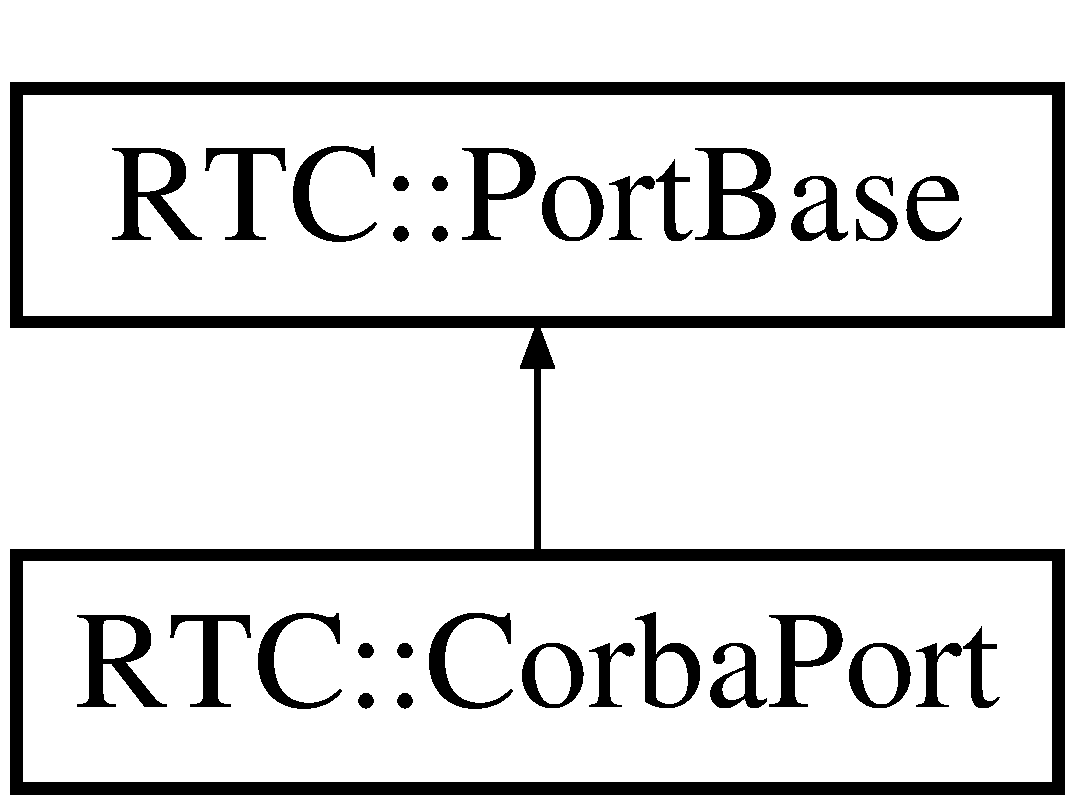
\includegraphics[height=2cm]{classRTC_1_1CorbaPort}
\end{center}
\end{figure}
\subsection*{Classes}
\begin{DoxyCompactItemize}
\item 
class {\bfseries CorbaConsumerHolder}
\begin{DoxyCompactList}\small\item\em The structure to be stored \doxyref{Consumer}{p.}{classConsumer} information. \item\end{DoxyCompactList}\item 
class {\bfseries CorbaProviderHolder}
\begin{DoxyCompactList}\small\item\em The structure to be stored Provider information. \item\end{DoxyCompactList}\item 
struct {\bfseries unsubscribe}
\begin{DoxyCompactList}\small\item\em Functor to release Consumer's object. \item\end{DoxyCompactList}\end{DoxyCompactItemize}
\subsection*{Public Member Functions}
\begin{DoxyCompactItemize}
\item 
{\bf CorbaPort} (const char $\ast$name)
\begin{DoxyCompactList}\small\item\em Constructor. \item\end{DoxyCompactList}\item 
virtual {\bf $\sim$CorbaPort} (void)
\begin{DoxyCompactList}\small\item\em Virtual destructor. \item\end{DoxyCompactList}\item 
void {\bf init} ({\bf coil::Properties} \&prop)
\begin{DoxyCompactList}\small\item\em Initializing properties. \item\end{DoxyCompactList}\item 
bool {\bf registerProvider} (const char $\ast$instance\_\-name, const char $\ast$type\_\-name, PortableServer::RefCountServantBase \&provider)
\begin{DoxyCompactList}\small\item\em Register the provider. \item\end{DoxyCompactList}\item 
bool {\bf registerConsumer} (const char $\ast$instance\_\-name, const char $\ast$type\_\-name, {\bf CorbaConsumerBase} \&consumer)
\begin{DoxyCompactList}\small\item\em Register the consumer. \item\end{DoxyCompactList}\end{DoxyCompactItemize}
\subsection*{Protected Member Functions}
\begin{DoxyCompactItemize}
\item 
virtual ReturnCode\_\-t {\bf publishInterfaces} (ConnectorProfile \&connector\_\-profile)
\begin{DoxyCompactList}\small\item\em Publish information about interfaces. \item\end{DoxyCompactList}\item 
virtual ReturnCode\_\-t {\bf subscribeInterfaces} (const ConnectorProfile \&connector\_\-profile)
\begin{DoxyCompactList}\small\item\em Subscribe to interface. \item\end{DoxyCompactList}\item 
virtual void {\bf unsubscribeInterfaces} (const ConnectorProfile \&connector\_\-profile)
\begin{DoxyCompactList}\small\item\em Unsubscribe interfaces. \item\end{DoxyCompactList}\item 
virtual void {\bf activateInterfaces} ()
\begin{DoxyCompactList}\small\item\em Activate all Port interfaces. \item\end{DoxyCompactList}\item 
virtual void {\bf deactivateInterfaces} ()
\begin{DoxyCompactList}\small\item\em Deactivate all Port interfaces. \item\end{DoxyCompactList}\end{DoxyCompactItemize}
\subsection*{Protected Attributes}
\begin{DoxyCompactItemize}
\item 
{\bf coil::Properties} {\bf m\_\-properties}
\begin{DoxyCompactList}\small\item\em Properties. \item\end{DoxyCompactList}\end{DoxyCompactItemize}


\subsection{Detailed Description}
RT Conponent CORBA service/consumer Port. \doxyref{CorbaPort}{p.}{classRTC_1_1CorbaPort} is an implementation of the Port of RT-\/Component's that provides user-\/defined CORBA Object Service and \doxyref{Consumer}{p.}{classConsumer}. 

RT-\/Component can provide user-\/defined CORBA serivces, which is called RT-\/Serivce (Provider), through the Ports. RT-\/Component can also provide place-\/holder, which is called RT-\/Serivce \doxyref{Consumer}{p.}{classConsumer}, to use other RT-\/Component's service. 

The \doxyref{CorbaPort}{p.}{classRTC_1_1CorbaPort} can manage any number of Providers and Consumers, can associate Consumers with correspondent Providers when establishing connection among Ports. 

Usually, \doxyref{CorbaPort}{p.}{classRTC_1_1CorbaPort} is used like the following.


\begin{DoxyPre}
 \doxyref{RTC::CorbaPort}{p.}{classRTC_1_1CorbaPort} m\_port0; // declaration of Port\end{DoxyPre}



\begin{DoxyPre} MyService\_impl m\_mysvc0; // Serivce Provider that is provided by the Port
 RTC::CorbaConsumer<YourService> m\_cons0; // \doxyref{Consumer}{p.}{classConsumer} of the Port\end{DoxyPre}



\begin{DoxyPre} // register Service Provider to the Port
 m\_port0.registerProvider("MyService0", "Generic", m\_mysvc0);
 // register Service \doxyref{Consumer}{p.}{classConsumer} to the Port
 m\_port0.registerConsumer("YourService0", "Generic", m\_cons0 );\end{DoxyPre}



\begin{DoxyPre} // after connect established\end{DoxyPre}



\begin{DoxyPre} m\_cons0->your\_service\_function(); // call a YourService's function\end{DoxyPre}



\begin{DoxyPre} // in another component that is connected with the Port
 m\_cons1->my\_service\_function(); // call a MyService's function
 \end{DoxyPre}


Registering Service Provider by \doxyref{registerProvider()}{p.}{classRTC_1_1CorbaPort_af9de5f6a90d3b0f6bfc07317e6a0d44f}, it can be used from other RT-\/Components. Registering Service \doxyref{Consumer}{p.}{classConsumer} by \doxyref{registerConsumer()}{p.}{classRTC_1_1CorbaPort_a70d4b49921c82916181aa681eea2ab2b}, other RT-\/Component's services can be used through the consumer object.

PortInterfaceProfile is a one of the profile information to store Provider interface and \doxyref{Consumer}{p.}{classConsumer} interface information. Tools or other RTCs should call one of the Port::connect() with an appropriate ConnectorProfile.

In addition, the instance name \char`\"{}$\ast$\char`\"{} declares a special type of instance.

When the name of the PROVIDED type interface that is the provider interface is \char`\"{}$\ast$\char`\"{}, Provider interface's instance does not exist at the beginning of connection sequence. The instances will be created dynamically according to the consumer interface requirement at the connection sequence. Although the instance name does not exist at the beginning of connection sequence, the created providers shall publish its references to the ConnectorProfile with interface descriptor adequately in the interface publisher phase of the connection sequence.

If REQUIRED interface name that is \doxyref{Consumer}{p.}{classConsumer} interface name is \char`\"{}$\ast$\char`\"{}, it shows that one \doxyref{Consumer}{p.}{classConsumer} interface is able to connect with multiple Provider interfaces. (This feature is not implemented.)

The following describes the rules that specify interface connection between ports.

The descriptor format of interfaces associated with Ports is declared as follows. Now some of interface properties are assumed as the followings.


\begin{DoxyItemize}
\item \doxyref{RTC}{p.}{namespaceRTC} instance name: rtc\_\-iname
\item Port name: port\_\-name
\item Interface polarity: if\_\-polarity
\item Interface type name: if\_\-tname
\item INterface instance name: if\_\-iname
\end{DoxyItemize}

The interface descriptors shall be declared as follows.

$<$rtc\_\-iname$>$.port.$<$port\_\-name$>$.$<$if\_\-polarity$>$.$<$if\_\-tname$>$.$<$if\_\-iname$>$

When PROVIDED that is Provider interface properties are the followings,


\begin{DoxyItemize}
\item rtc\_\-iname = MyComp0
\item port\_\-name = myservice
\item if\_\-polarity = provided
\item if\_\-tname = echo\_\-interface
\item if\_\-iname = echo\_\-interface2 the interface descriptor is here.
\end{DoxyItemize}

MyComp0.port.myservice.provided.echo\_\-interface.echo\_\-interface2

And, when REQUIRED that is \doxyref{Consumer}{p.}{classConsumer} interfaces properties are the followings,


\begin{DoxyItemize}
\item rtc\_\-iname = YourComp0
\item port\_\-name = yourservice
\item if\_\-polarity = required
\item if\_\-tname = hoge\_\-interface
\item if\_\-iname = hoge\_\-interface1
\end{DoxyItemize}

interface descriptor is as follows.

YourComp0.port.myservice.required.hoge\_\-interface.hoge\_\-inteface1

Specific instance name descriptors that are dynamically generated at the connection time are defined here.


\begin{DoxyItemize}
\item $<$type\_\-name$>$$\ast$: \char`\"{}Dynamically generated\char`\"{} instance descriptor.
\item $<$type\_\-name$>$+: \char`\"{}Incrementally generated\char`\"{} instance descriptor.
\end{DoxyItemize}

When the \char`\"{}Dynamically generated\char`\"{} instance descriptor: \char`\"{}$<$type\_\-name$>$$\ast$\char`\"{} is specified as interface descriptor that is required by consumers, the provider will generate a instance. If n consumers who demand a provider by the \char`\"{}$<$type\_\-name$>$\char`\"{} descriptor exist, the following relation which processes the call from these consumers by one provider will be established.


\begin{DoxyPre}
 consumer0 ]---<
 consumer1 ]---<  O----[ provider0
 consumer2 ]---<
 \end{DoxyPre}


On the other hand, when incremental generated type instance name descriptor \char`\"{}$<$type\_\-name$>$+\char`\"{} is specified as the provider interface descriptor whom consumers demand, provider's instances are dynamically generated for the number of the descriptors \char`\"{}$<$type\_\-name$>$+\char`\"{}. When n consumers who demand a provider by the descriptor \char`\"{}$<$type\_\-name$>$+\char`\"{} exist the following relations in which n providers process each call from the consumers will be established.


\begin{DoxyPre}
 consumer0 ]---<  O----[ provider0
 consumer1 ]---<  O----[ provider1
 consumer2 ]---<  O----[ provider2
 \end{DoxyPre}


Describing the appropriate interface mapping specification in the ConnectorProfile::properties, selective connections between providers/consumers interface can be established at the time of connection. However, when different \doxyref{RTC}{p.}{namespaceRTC} instances of the same instance name exist in a connection, since an interface descriptor uniqueness cannot be guaranteed, this connection mapping rules cannot be used.

Here, assume that an interface descriptor is given as $<$if\_\-desc0$>$, $<$if\_\-desc1$>$, .... And assume that the key and the value of NVList in ConnectorProfile::properties are given as \char`\"{}key: value\char`\"{}.

Now the case where the service ports of two components are connected is considered. When the service port of each component is the following,


\begin{DoxyItemize}
\item rtc\_\-iname: MyComp0 \par
 port\_\-name: mycomp\_\-service \par
 interfaces:
\begin{DoxyItemize}
\item if\_\-polarity: provided \par
 if\_\-iname: echo0 \par
 if\_\-tname: Echo
\item if\_\-polarity: required \par
 if\_\-iname: add0 \par
 if\_\-tname: add
\end{DoxyItemize}
\end{DoxyItemize}


\begin{DoxyItemize}
\item rtc\_\-iname: YourComp0 \par
 port\_\-name: yourcomp\_\-service \par
 interfaces:
\begin{DoxyItemize}
\item if\_\-polarity: required \par
 if\_\-iname: echo9 \par
 if\_\-tname: Echo
\item if\_\-polarity: provided \par
 if\_\-iname: add9 \par
 if\_\-tname: add
\end{DoxyItemize}
\end{DoxyItemize}


\begin{DoxyPre}
      MyComp0                                 YourComp0
     \_\_\_\_\_\_\_ mycomp\_service   yourcomp\_service \_\_\_\_\_\_
            |                                 |
          |~~~|---O echo0         echo9 >---|~~~|
          |   |---< add0          add9  O---|   |
           ~T~                               ~T~
            |                                 |
 \end{DoxyPre}


Assume that connection between echo0 (provider) of MyComp0 component and echo9 (consumer) of YourComp0 component, and add0 (consumer) of MyComp0 and add0 (provider) of YourComp0 is established. In this case, ConnectorProfile is set up as follows.


\begin{DoxyPre}
 ConnectorProfile:
   name: any connector name
   connector\_id: empty string
   ports[]: mycomp\_service's reference, yourcomp\_service's reference
   properties:
     <add0>: <add9>
     <echo9>: <echo0>
 \end{DoxyPre}


Please note that $<$add0$>$, $<$add9$>$, $<$echo0$>$ and $<$echo9$>$ are the following.


\begin{DoxyPre}
 <add0> is MyComp0.port.mycomp\_service.required.add.add0
 <add9> is YourComp0.port.yourcomp\_service.provided.add.add9
 <echo0> is MyComp0.port.mycomp\_service.provided.echo.echo0
 <echo9> is YourComp0.port.yourcomp\_service.required.echo.echo9
 \end{DoxyPre}


In the connection process, the provider and the consumer of each port carries out the following process respectively in the virtual functions such as \doxyref{CorbaPort::publishInterfaces()}{p.}{classRTC_1_1CorbaPort_a71aa316c3324369c4462193d10a5d098} and CorbaPort::subscribeInerfaces().

A provider sets its IOR string as a value and its interface descriptor as a key in the ConnectorProfile::properties in a \doxyref{publishInterfaces()}{p.}{classRTC_1_1CorbaPort_a71aa316c3324369c4462193d10a5d098} function. Since this interface descriptor's uniqueness is guaranteed in the current connector, the key of NameValue in the ConnectorProfile::properties is unique.

[This functionalities are not implemented] The dynamically generated provider is processed according to the following procedure. The publishInterface() function scans dynamic instance descriptors such as \char`\"{}$<$type\_\-name$>$$\ast$\char`\"{} and \char`\"{}$<$type\_\-name$>$+\char`\"{} in the ConnectorProfile::properties. When the dynamic generation instance descriptor \char`\"{}$<$tupe\_\-name$>$$\ast$\char`\"{} exists, one instance of provider is generated, and its descriptor and its IOR string are set to ConnectorProfile::properties as the key and the value respectively. Simultaneously, in the ConnectorProfile::properties, all the instance descriptor with the dynamic generation instance name \char`\"{}$<$type\_\-name$>$$\ast$\char`\"{} will be replaced with newly generated instance descriptor.

When the incremental dynamic generation instance descriptor exists, providers are generated for the number of the descriptors, and its descriptor and its IOR string are set to ConnectorProfile::properties as the key and the value respectively. Simultaneously, in the ConnectorProfile::properties, all the instance descriptor with the dynamic generation instance name \char`\"{}$<$type\_\-name$>$+\char`\"{} will be replaced with newly generated instance descriptor.

The providers do not perform particular operation in \doxyref{subscribeInterfaces()}{p.}{classRTC_1_1CorbaPort_ad9a122cbe2f9892cc9555e805571742e} function.

The consumers do not perform particular operation in publisherInterfaces() function.

On the other hand, a consumer searches a key-\/value pair with the key of consumer interface descriptor, and if the pair exists, it obtains provider's descriptor from the value. The consumer searches again a key-\/value pair with the key of provider interface descriptor, and it obtains provider's reference and the reference is set as the consumer's service object. In addition, reserved string \char`\"{}nil\char`\"{} or \char`\"{}null\char`\"{} are used not to set specific provider.

If consumer's interface descriptors does not exists in the ConnectorProfile::properties, the consumer searches a provider with same type name and instance name, and its reference is set to the consumer. This rule is for only backward compatibility, and it is not recommended from version 1.0.

The correspondence of a provider versus a consumer does not need to be one to one, and the case of one provider to n-\/consumers and the case of m-\/providers to one consumer are allowed. The one provider to n-\/consumers case can be realized by the above mentioned methods. The one consumer to m-\/provider case can be specified to set the consumer descriptor and comma-\/separated provider descriptors into the key and the value respectively.

The following option is available to specify the strictness of interfaces connection.

port.connection.strictness: strict, best\_\-effort

strict: The connection is established, if only all the specified consumers are set appropriate references and narrowed successfully.

best\_\-effort: The connection is established without any errors, even if appropriate reference does not exist or reference narrowing fails.

\begin{DoxySince}{Since}
0.4.0 
\end{DoxySince}


\subsection{Constructor \& Destructor Documentation}
\index{RTC::CorbaPort@{RTC::CorbaPort}!CorbaPort@{CorbaPort}}
\index{CorbaPort@{CorbaPort}!RTC::CorbaPort@{RTC::CorbaPort}}
\subsubsection[{CorbaPort}]{\setlength{\rightskip}{0pt plus 5cm}RTC::CorbaPort::CorbaPort (const char $\ast$ {\em name})}\label{classRTC_1_1CorbaPort_a2bbb2b39d9df5f82c61315fe3fa5cf7a}


Constructor. 

In the ctor, a given name is set into \doxyref{PortBase}{p.}{classRTC_1_1PortBase}, and the following property is added to the PortProfile::properties,


\begin{DoxyItemize}
\item port.port\_\-type: \char`\"{}CorbaPort\char`\"{}
\end{DoxyItemize}


\begin{DoxyParams}{Parameters}
\item[{\em name}]The name of Port \end{DoxyParams}
\index{RTC::CorbaPort@{RTC::CorbaPort}!$\sim$CorbaPort@{$\sim$CorbaPort}}
\index{$\sim$CorbaPort@{$\sim$CorbaPort}!RTC::CorbaPort@{RTC::CorbaPort}}
\subsubsection[{$\sim$CorbaPort}]{\setlength{\rightskip}{0pt plus 5cm}virtual RTC::CorbaPort::$\sim$CorbaPort (void)\hspace{0.3cm}{\ttfamily  [virtual]}}\label{classRTC_1_1CorbaPort_a7aa53f50989ea68ca419b9f6d5a8cfcc}


Virtual destructor. 



\subsection{Member Function Documentation}
\index{RTC::CorbaPort@{RTC::CorbaPort}!activateInterfaces@{activateInterfaces}}
\index{activateInterfaces@{activateInterfaces}!RTC::CorbaPort@{RTC::CorbaPort}}
\subsubsection[{activateInterfaces}]{\setlength{\rightskip}{0pt plus 5cm}virtual void RTC::CorbaPort::activateInterfaces ()\hspace{0.3cm}{\ttfamily  [protected, virtual]}}\label{classRTC_1_1CorbaPort_a1b9efe804a293b2c38a9cbe3b5ba54a0}


Activate all Port interfaces. 

This operation activate all interfaces that is registered in the ports. 

Implements {\bf RTC::PortBase} \doxyref{}{p.}{classRTC_1_1PortBase_ad779347bae007555968dda9e78004e34}.

\index{RTC::CorbaPort@{RTC::CorbaPort}!deactivateInterfaces@{deactivateInterfaces}}
\index{deactivateInterfaces@{deactivateInterfaces}!RTC::CorbaPort@{RTC::CorbaPort}}
\subsubsection[{deactivateInterfaces}]{\setlength{\rightskip}{0pt plus 5cm}virtual void RTC::CorbaPort::deactivateInterfaces ()\hspace{0.3cm}{\ttfamily  [protected, virtual]}}\label{classRTC_1_1CorbaPort_a4c25f8e04aa9cceff24c31ea3fec4e5b}


Deactivate all Port interfaces. 

This operation deactivate all interfaces that is registered in the ports. 

Implements {\bf RTC::PortBase} \doxyref{}{p.}{classRTC_1_1PortBase_a8dfb8a33b92b9fc9b6c070df2def633f}.

\index{RTC::CorbaPort@{RTC::CorbaPort}!init@{init}}
\index{init@{init}!RTC::CorbaPort@{RTC::CorbaPort}}
\subsubsection[{init}]{\setlength{\rightskip}{0pt plus 5cm}void RTC::CorbaPort::init ({\bf coil::Properties} \& {\em prop})}\label{classRTC_1_1CorbaPort_a5e62ee7818cafc02a3e7002a3742daab}


Initializing properties. 

This operation initializes outport's properties. If a property \char`\"{}connection\_\-limit\char`\"{} is set and appropriate value is set to this property value, the number of maximum connection is set as this value. If the property does not exist or invalid value is set to this property, the maximum number of connection will be set unlimited.


\begin{DoxyParams}{Parameters}
\item[{\em prop}]properties of the \doxyref{CorbaPort}{p.}{classRTC_1_1CorbaPort} \end{DoxyParams}
\index{RTC::CorbaPort@{RTC::CorbaPort}!publishInterfaces@{publishInterfaces}}
\index{publishInterfaces@{publishInterfaces}!RTC::CorbaPort@{RTC::CorbaPort}}
\subsubsection[{publishInterfaces}]{\setlength{\rightskip}{0pt plus 5cm}virtual ReturnCode\_\-t RTC::CorbaPort::publishInterfaces (ConnectorProfile \& {\em connector\_\-profile})\hspace{0.3cm}{\ttfamily  [protected, virtual]}}\label{classRTC_1_1CorbaPort_a71aa316c3324369c4462193d10a5d098}


Publish information about interfaces. 

This operation publishes Provider interfaces information, which is owned by this port, to the other Ports via ConnectorProfile::properties. Now it is assumed \doxyref{RTC}{p.}{namespaceRTC} instance name and other information is as follows,


\begin{DoxyItemize}
\item \doxyref{RTC}{p.}{namespaceRTC} instance name: rtc\_\-iname
\item Port name: port\_\-name
\item Interface polarity: if\_\-polarity
\item Interface type name: if\_\-tname
\item Interface instance name: if\_\-iname
\end{DoxyItemize}

the following values are stored as the \char`\"{}name\char`\"{} and the \char`\"{}value\char`\"{} of the NameValue typee element in ConnectorProfile::properties.


\begin{DoxyItemize}
\item name $<$rtc\_\-iname$>$.port.$<$port\_\-name$>$.provided.$<$if\_\-tname$>$.$<$if\_\-iname$>$
\item value IOR string value of interface reference
\end{DoxyItemize}

In addition, although the following NameValue values are also stored for the backward compatibility, this will be deleted in the future version.


\begin{DoxyItemize}
\item name port.$<$if\_\-tname$>$.$<$if\_\-iname$>$
\item value IOR string value of interface reference
\end{DoxyItemize}

These values are stored in the ConnectorProfile::properties and are propagated to the other Ports. If the \doxyref{Consumer}{p.}{classConsumer} interface exists that requires this Provider interface, it will retrieve reference from the ConnectorProfile and utilize it.


\begin{DoxyParams}{Parameters}
\item[{\em connector\_\-profile}]Connector profile \end{DoxyParams}
\begin{DoxyReturn}{Returns}
The return code of ReturnCode\_\-t type 
\end{DoxyReturn}


Implements {\bf RTC::PortBase} \doxyref{}{p.}{classRTC_1_1PortBase_acf31878c5912f56c122aaa2310e182de}.

\index{RTC::CorbaPort@{RTC::CorbaPort}!registerConsumer@{registerConsumer}}
\index{registerConsumer@{registerConsumer}!RTC::CorbaPort@{RTC::CorbaPort}}
\subsubsection[{registerConsumer}]{\setlength{\rightskip}{0pt plus 5cm}bool RTC::CorbaPort::registerConsumer (const char $\ast$ {\em instance\_\-name}, \/  const char $\ast$ {\em type\_\-name}, \/  {\bf CorbaConsumerBase} \& {\em consumer})}\label{classRTC_1_1CorbaPort_a70d4b49921c82916181aa681eea2ab2b}


Register the consumer. 

This operation registers a consumer, which is a service placeholder this port requires. These are associated internally with specified instance\_\-name, type\_\-name and \doxyref{Consumer}{p.}{classConsumer} itself to the argument as service's instance name and its type name associated with \doxyref{Consumer}{p.}{classConsumer}. The service Provider interface' references will be set automatically to the \doxyref{Consumer}{p.}{classConsumer} Interface object when connections are established, according to the rules that are described at the subscribeInterface() function's documentation.


\begin{DoxyParams}{Parameters}
\item[{\em instance\_\-name}]Instance name of the service \doxyref{Consumer}{p.}{classConsumer} requires \item[{\em type\_\-name}]Type name of the service \doxyref{Consumer}{p.}{classConsumer} requires \item[{\em consumer}]CORBA service consumer\end{DoxyParams}
\begin{DoxyReturn}{Returns}
False would be returned if the same instance\_\-name was registered 
\end{DoxyReturn}
\index{RTC::CorbaPort@{RTC::CorbaPort}!registerProvider@{registerProvider}}
\index{registerProvider@{registerProvider}!RTC::CorbaPort@{RTC::CorbaPort}}
\subsubsection[{registerProvider}]{\setlength{\rightskip}{0pt plus 5cm}bool RTC::CorbaPort::registerProvider (const char $\ast$ {\em instance\_\-name}, \/  const char $\ast$ {\em type\_\-name}, \/  PortableServer::RefCountServantBase \& {\em provider})}\label{classRTC_1_1CorbaPort_af9de5f6a90d3b0f6bfc07317e6a0d44f}


Register the provider. 

This operation registers a servant, which is provided in this Port, to the Port. The servant is associated with \char`\"{}instance\_\-name\char`\"{} and \char`\"{}type\_\-name\char`\"{} as the instance name of the servant and as the type name of the servant. A given servant will be stored in the \doxyref{CorbaPort}{p.}{classRTC_1_1CorbaPort}, and this is registered as RTC::PROVIDED interface into the PortInterfaceProfile.


\begin{DoxyParams}{Parameters}
\item[{\em instance\_\-name}]Instance name of servant \item[{\em type\_\-name}]Type name of the servant \item[{\em provider}]CORBA servant\end{DoxyParams}
\begin{DoxyReturn}{Returns}
Return false if the same name of instance\_\-name is already registered. 
\end{DoxyReturn}
\index{RTC::CorbaPort@{RTC::CorbaPort}!subscribeInterfaces@{subscribeInterfaces}}
\index{subscribeInterfaces@{subscribeInterfaces}!RTC::CorbaPort@{RTC::CorbaPort}}
\subsubsection[{subscribeInterfaces}]{\setlength{\rightskip}{0pt plus 5cm}virtual ReturnCode\_\-t RTC::CorbaPort::subscribeInterfaces (const ConnectorProfile \& {\em connector\_\-profile})\hspace{0.3cm}{\ttfamily  [protected, virtual]}}\label{classRTC_1_1CorbaPort_ad9a122cbe2f9892cc9555e805571742e}


Subscribe to interface. 

Retrieve information associated with Provider matches \doxyref{Consumer}{p.}{classConsumer} owned by this port and set the object reference to \doxyref{Consumer}{p.}{classConsumer}.

Now, \doxyref{Consumer}{p.}{classConsumer} is registered as the following: 
\begin{DoxyPre}
  PortInterfaceProfile
  \{
    instance\_name = "PA10\_0";
    type\_name     = "Manipulator";
    polarity      = REQUIRED;
  \}
 \end{DoxyPre}
 Find the object reference of Serivce Provider that is registered as the following of other ports: 
\begin{DoxyPre}
  PortInterfaceProfile
  \{
    instance\_name = "PA10\_0";
    type\_name     = "Manipulator";
    polarity      = PROVIDED;
  \}
 \end{DoxyPre}
 and set to \doxyref{Consumer}{p.}{classConsumer}. In fact, find NameValue that is registered as the following to ConnectorProfile::properties: 
\begin{DoxyPre}
 NameValue = \{ "port.Manipulator.PA10\_0": <Object reference>=""> \}
 \end{DoxyPre}
 and set the object reference to \doxyref{Consumer}{p.}{classConsumer}.


\begin{DoxyParams}{Parameters}
\item[{\em connector\_\-profile}]Connector profile\end{DoxyParams}
\begin{DoxyReturn}{Returns}
The return code of ReturnCode\_\-t type 
\end{DoxyReturn}


Implements {\bf RTC::PortBase} \doxyref{}{p.}{classRTC_1_1PortBase_afce755069836c1ee637784e2a9e5a02b}.

\index{RTC::CorbaPort@{RTC::CorbaPort}!unsubscribeInterfaces@{unsubscribeInterfaces}}
\index{unsubscribeInterfaces@{unsubscribeInterfaces}!RTC::CorbaPort@{RTC::CorbaPort}}
\subsubsection[{unsubscribeInterfaces}]{\setlength{\rightskip}{0pt plus 5cm}virtual void RTC::CorbaPort::unsubscribeInterfaces (const ConnectorProfile \& {\em connector\_\-profile})\hspace{0.3cm}{\ttfamily  [protected, virtual]}}\label{classRTC_1_1CorbaPort_a4776e122a3066d9e3a3e5d1e5da45b98}


Unsubscribe interfaces. 

Release all Objects that was set in \doxyref{Consumer}{p.}{classConsumer} associated with the given ConnectorProfile.


\begin{DoxyParams}{Parameters}
\item[{\em connector\_\-profile}]Connector profile \end{DoxyParams}


Implements {\bf RTC::PortBase} \doxyref{}{p.}{classRTC_1_1PortBase_a8a843a387e99d4d4daa6e829eb1db569}.



\subsection{Member Data Documentation}
\index{RTC::CorbaPort@{RTC::CorbaPort}!m\_\-properties@{m\_\-properties}}
\index{m\_\-properties@{m\_\-properties}!RTC::CorbaPort@{RTC::CorbaPort}}
\subsubsection[{m\_\-properties}]{\setlength{\rightskip}{0pt plus 5cm}{\bf coil::Properties} {\bf RTC::CorbaPort::m\_\-properties}\hspace{0.3cm}{\ttfamily  [protected]}}\label{classRTC_1_1CorbaPort_afb24858ffd644ff6d52bb422cfb442da}


Properties. 


\section{クラス RTC::DataFlowComponentBase}
\label{classRTC_1_1DataFlowComponentBase}\index{RTC::DataFlowComponentBase@{RTC::DataFlowComponentBase}}


\doxyref{DataFlowComponentBase}{p.}{classRTC_1_1DataFlowComponentBase} クラス.  




{\ttfamily \#include $<$DataFlowComponentBase.h$>$}

RTC::DataFlowComponentBaseに対する継承グラフ\begin{figure}[H]
\begin{center}
\leavevmode
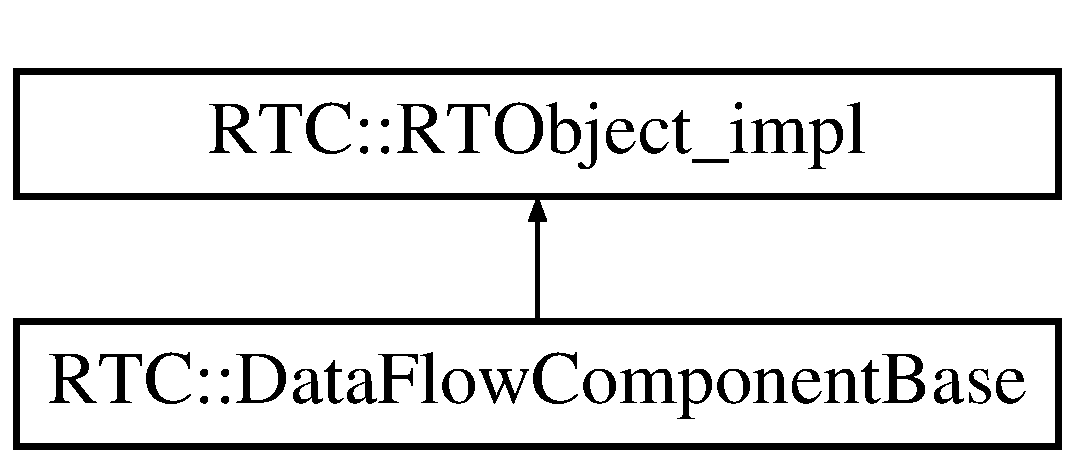
\includegraphics[height=2cm]{classRTC_1_1DataFlowComponentBase}
\end{center}
\end{figure}
\subsection*{Public メソッド}
\begin{DoxyCompactItemize}
\item 
{\bf DataFlowComponentBase} ({\bf Manager} $\ast$manager)
\begin{DoxyCompactList}\small\item\em コンストラクタ \item\end{DoxyCompactList}\item 
virtual {\bf $\sim$DataFlowComponentBase} (void)
\item 
void {\bf init} ()
\begin{DoxyCompactList}\small\item\em 初期化 \item\end{DoxyCompactList}\end{DoxyCompactItemize}


\subsection{説明}
\doxyref{DataFlowComponentBase}{p.}{classRTC_1_1DataFlowComponentBase} クラス. データフロー型RTComponentの基底クラス。 各種データフロー型RTComponentを実装する場合は、本クラスを継承する形で実装 する。

\begin{DoxySince}{から}
0.4.0 
\end{DoxySince}


\subsection{コンストラクタとデストラクタ}
\index{RTC::DataFlowComponentBase@{RTC::DataFlowComponentBase}!DataFlowComponentBase@{DataFlowComponentBase}}
\index{DataFlowComponentBase@{DataFlowComponentBase}!RTC::DataFlowComponentBase@{RTC::DataFlowComponentBase}}
\subsubsection[{DataFlowComponentBase}]{\setlength{\rightskip}{0pt plus 5cm}RTC::DataFlowComponentBase::DataFlowComponentBase ({\bf Manager} $\ast$ {\em manager})}\label{classRTC_1_1DataFlowComponentBase_ac93dffa99b69b93f382aac906f8591ae}


コンストラクタ 

コンストラクタ


\begin{DoxyParams}{引数}
\item[{\em manager}]マネージャオブジェクト \end{DoxyParams}
\index{RTC::DataFlowComponentBase@{RTC::DataFlowComponentBase}!$\sim$DataFlowComponentBase@{$\sim$DataFlowComponentBase}}
\index{$\sim$DataFlowComponentBase@{$\sim$DataFlowComponentBase}!RTC::DataFlowComponentBase@{RTC::DataFlowComponentBase}}
\subsubsection[{$\sim$DataFlowComponentBase}]{\setlength{\rightskip}{0pt plus 5cm}virtual RTC::DataFlowComponentBase::$\sim$DataFlowComponentBase (void)\hspace{0.3cm}{\ttfamily  [virtual]}}\label{classRTC_1_1DataFlowComponentBase_aefcb5d65ed4ccac35e20cf8caa17c279}
デストラクタ 

\subsection{関数}
\index{RTC::DataFlowComponentBase@{RTC::DataFlowComponentBase}!init@{init}}
\index{init@{init}!RTC::DataFlowComponentBase@{RTC::DataFlowComponentBase}}
\subsubsection[{init}]{\setlength{\rightskip}{0pt plus 5cm}void RTC::DataFlowComponentBase::init ()}\label{classRTC_1_1DataFlowComponentBase_aaab8d77b9eddf9fe6ccb321d5bcef4f4}


初期化 

データフロー型 RTComponent の初期化を実行する。 実際の初期化処理は、各具象クラス内に記述する。 
\section{RTC::DataPortStatus Class Reference}
\label{classRTC_1_1DataPortStatus}\index{RTC::DataPortStatus@{RTC::DataPortStatus}}


\doxyref{DataPortStatus}{p.}{classRTC_1_1DataPortStatus} mixin class.  




{\ttfamily \#include $<$DataPortStatus.h$>$}

Inheritance diagram for RTC::DataPortStatus:\begin{figure}[H]
\begin{center}
\leavevmode
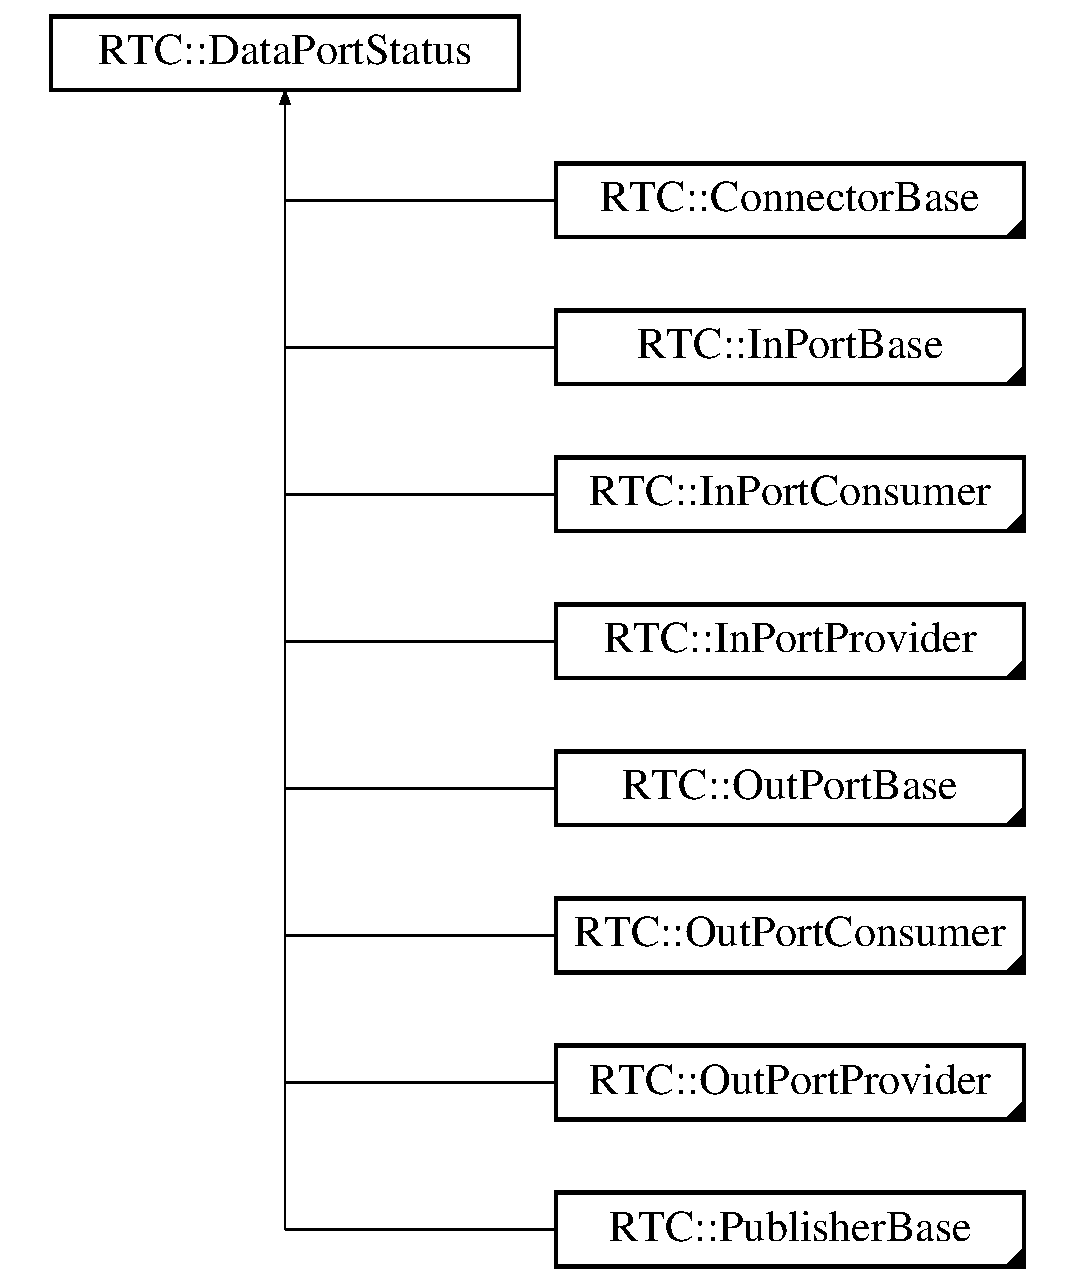
\includegraphics[height=9cm]{classRTC_1_1DataPortStatus}
\end{center}
\end{figure}
\subsection*{Public Types}
\begin{DoxyCompactItemize}
\item 
enum {\bf Enum} \{ \par
{\bf PORT\_\-OK} =  0, 
{\bf PORT\_\-ERROR}, 
{\bf BUFFER\_\-ERROR}, 
{\bf BUFFER\_\-FULL}, 
\par
{\bf BUFFER\_\-EMPTY}, 
{\bf BUFFER\_\-TIMEOUT}, 
{\bf SEND\_\-FULL}, 
{\bf SEND\_\-TIMEOUT}, 
\par
{\bf RECV\_\-EMPTY}, 
{\bf RECV\_\-TIMEOUT}, 
{\bf INVALID\_\-ARGS}, 
{\bf PRECONDITION\_\-NOT\_\-MET}, 
\par
{\bf CONNECTION\_\-LOST}, 
{\bf UNKNOWN\_\-ERROR}
 \}
\begin{DoxyCompactList}\small\item\em \doxyref{DataPortStatus}{p.}{classRTC_1_1DataPortStatus} return codes. \item\end{DoxyCompactList}\end{DoxyCompactItemize}
\subsection*{Static Public Member Functions}
\begin{DoxyCompactItemize}
\item 
static const char $\ast$ {\bf toString} ({\bf DataPortStatus::Enum} status)
\begin{DoxyCompactList}\small\item\em Convert \doxyref{DataPortStatus}{p.}{classRTC_1_1DataPortStatus} into the string. \item\end{DoxyCompactList}\end{DoxyCompactItemize}


\subsection{Detailed Description}
\doxyref{DataPortStatus}{p.}{classRTC_1_1DataPortStatus} mixin class. This is a mixin class to provide enumed return codes that are commonly utilised in data port related sub-\/classes. To use this class, sub-\/class should inherit this class as a public super class, and declare DATAPORTSTATUS\_\-ENUM defined below. Consequently, ReturnCode\_\-t type that is typedefed by this macro can be used in the sub-\/class, and enumed identifiers are imported to the class's namespace. 

\subsection{Member Enumeration Documentation}
\index{RTC::DataPortStatus@{RTC::DataPortStatus}!Enum@{Enum}}
\index{Enum@{Enum}!RTC::DataPortStatus@{RTC::DataPortStatus}}
\subsubsection[{Enum}]{\setlength{\rightskip}{0pt plus 5cm}enum {\bf RTC::DataPortStatus::Enum}}\label{classRTC_1_1DataPortStatus_ac47c3e85f39e51eb55230337c0efc64f}


\doxyref{DataPortStatus}{p.}{classRTC_1_1DataPortStatus} return codes. 

Common return codes for data ports related classes.


\begin{DoxyItemize}
\item PORT\_\-OK: Normal return
\item PORT\_\-ERROR: Error return
\item BUFFER\_\-ERROR: Buffer error
\item BUFFER\_\-FULL: Buffer full
\item BUFFER\_\-EMPTY: Buffer empty
\item BUFFER\_\-TIMEOUT: Buffer timeout
\item SEND\_\-FULL: Buffer full although \doxyref{OutPort}{p.}{classRTC_1_1OutPort} tried to send data
\item SEND\_\-TIMEOUT: Timeout although \doxyref{OutPort}{p.}{classRTC_1_1OutPort} tried to send data
\item RECV\_\-EMPTY: Buffer empty although \doxyref{InPort}{p.}{classRTC_1_1InPort} tried to receive data
\item RECV\_\-TIMEOUT: Timeout although \doxyref{InPort}{p.}{classRTC_1_1InPort} tried to receive data
\item INVALID\_\-ARGS: Invalid arguments
\item PRECONDITION\_\-NOT\_\-MET: Precondition not met
\item CONNECTION\_\-LOST: Connection has been lost
\item UNKNOWN\_\-ERROR: Unknown error
\end{DoxyItemize}

This error codes might be used to propagate error status from the error occurring point to the function caller in the data stream path. It would occur in data-\/transfer path and data receiver/sender. The errors that occur in the interface of each portion of data port are shown below.

(1) Push Type a) The return codes between \doxyref{InPortConsumer}{p.}{classRTC_1_1InPortConsumer} and Publisher/Activity PORT\_\-OK, PORT\_\-ERROR, SEND\_\-FULL, SEND\_\-TIMEOUT, CONNECTION\_\-LOST, UNKNOWN\_\-ERROR b) The return codes between Activity and Buffer/Connector of \doxyref{OutPort}{p.}{classRTC_1_1OutPort} PORT\_\-OK, PORT\_\-ERROR, BUFFER\_\-ERROR, BUFFER\_\-FULL, BUFFER\_\-TIMEOUT, UNKNOWN\_\-ERROR,

(2) Pull Type a) The return codes between Activity and \doxyref{InPort}{p.}{classRTC_1_1InPort} PORT\_\-OK, PORT\_\-ERROR, RECV\_\-EMPTY, RECV\_\-TIMEOUT, CONNETION\_\-LOST, UNKNOWN\_\-ERROR

See function references for detailed return codes for each function. \begin{Desc}
\item[Enumerator: ]\par
\begin{description}
\index{PORT\_\-OK@{PORT\_\-OK}!RTC::DataPortStatus@{RTC::DataPortStatus}}\index{RTC::DataPortStatus@{RTC::DataPortStatus}!PORT\_\-OK@{PORT\_\-OK}}\item[{\em 
PORT\_\-OK\label{classRTC_1_1DataPortStatus_ac47c3e85f39e51eb55230337c0efc64fa348f113d004fb38d3f95c1a6f0b39536}
}]\index{PORT\_\-ERROR@{PORT\_\-ERROR}!RTC::DataPortStatus@{RTC::DataPortStatus}}\index{RTC::DataPortStatus@{RTC::DataPortStatus}!PORT\_\-ERROR@{PORT\_\-ERROR}}\item[{\em 
PORT\_\-ERROR\label{classRTC_1_1DataPortStatus_ac47c3e85f39e51eb55230337c0efc64fa6f4b21b97192228ba0cccd1db472193f}
}]\index{BUFFER\_\-ERROR@{BUFFER\_\-ERROR}!RTC::DataPortStatus@{RTC::DataPortStatus}}\index{RTC::DataPortStatus@{RTC::DataPortStatus}!BUFFER\_\-ERROR@{BUFFER\_\-ERROR}}\item[{\em 
BUFFER\_\-ERROR\label{classRTC_1_1DataPortStatus_ac47c3e85f39e51eb55230337c0efc64fac15043a37b27327bd4125fe07a23ffcb}
}]\index{BUFFER\_\-FULL@{BUFFER\_\-FULL}!RTC::DataPortStatus@{RTC::DataPortStatus}}\index{RTC::DataPortStatus@{RTC::DataPortStatus}!BUFFER\_\-FULL@{BUFFER\_\-FULL}}\item[{\em 
BUFFER\_\-FULL\label{classRTC_1_1DataPortStatus_ac47c3e85f39e51eb55230337c0efc64fa468123dd45be6af47fc7b059d7bc408f}
}]\index{BUFFER\_\-EMPTY@{BUFFER\_\-EMPTY}!RTC::DataPortStatus@{RTC::DataPortStatus}}\index{RTC::DataPortStatus@{RTC::DataPortStatus}!BUFFER\_\-EMPTY@{BUFFER\_\-EMPTY}}\item[{\em 
BUFFER\_\-EMPTY\label{classRTC_1_1DataPortStatus_ac47c3e85f39e51eb55230337c0efc64fac70e9db863797db8202eb552ee380e3f}
}]\index{BUFFER\_\-TIMEOUT@{BUFFER\_\-TIMEOUT}!RTC::DataPortStatus@{RTC::DataPortStatus}}\index{RTC::DataPortStatus@{RTC::DataPortStatus}!BUFFER\_\-TIMEOUT@{BUFFER\_\-TIMEOUT}}\item[{\em 
BUFFER\_\-TIMEOUT\label{classRTC_1_1DataPortStatus_ac47c3e85f39e51eb55230337c0efc64fa07801b7d1af39c7e9b2fb0a0b5f103b8}
}]\index{SEND\_\-FULL@{SEND\_\-FULL}!RTC::DataPortStatus@{RTC::DataPortStatus}}\index{RTC::DataPortStatus@{RTC::DataPortStatus}!SEND\_\-FULL@{SEND\_\-FULL}}\item[{\em 
SEND\_\-FULL\label{classRTC_1_1DataPortStatus_ac47c3e85f39e51eb55230337c0efc64fad447808595a3ab498eaf987e4d1111ad}
}]\index{SEND\_\-TIMEOUT@{SEND\_\-TIMEOUT}!RTC::DataPortStatus@{RTC::DataPortStatus}}\index{RTC::DataPortStatus@{RTC::DataPortStatus}!SEND\_\-TIMEOUT@{SEND\_\-TIMEOUT}}\item[{\em 
SEND\_\-TIMEOUT\label{classRTC_1_1DataPortStatus_ac47c3e85f39e51eb55230337c0efc64fa740d85b9b7a2519c8e309bcb265c1da0}
}]\index{RECV\_\-EMPTY@{RECV\_\-EMPTY}!RTC::DataPortStatus@{RTC::DataPortStatus}}\index{RTC::DataPortStatus@{RTC::DataPortStatus}!RECV\_\-EMPTY@{RECV\_\-EMPTY}}\item[{\em 
RECV\_\-EMPTY\label{classRTC_1_1DataPortStatus_ac47c3e85f39e51eb55230337c0efc64fa2df59b07f60ecb05b80d76149318cd9a}
}]\index{RECV\_\-TIMEOUT@{RECV\_\-TIMEOUT}!RTC::DataPortStatus@{RTC::DataPortStatus}}\index{RTC::DataPortStatus@{RTC::DataPortStatus}!RECV\_\-TIMEOUT@{RECV\_\-TIMEOUT}}\item[{\em 
RECV\_\-TIMEOUT\label{classRTC_1_1DataPortStatus_ac47c3e85f39e51eb55230337c0efc64fa6890d025dc4c9eee20a90371f01d1fa7}
}]\index{INVALID\_\-ARGS@{INVALID\_\-ARGS}!RTC::DataPortStatus@{RTC::DataPortStatus}}\index{RTC::DataPortStatus@{RTC::DataPortStatus}!INVALID\_\-ARGS@{INVALID\_\-ARGS}}\item[{\em 
INVALID\_\-ARGS\label{classRTC_1_1DataPortStatus_ac47c3e85f39e51eb55230337c0efc64fab564856fd2ed7c6f013a2153aa69b3df}
}]\index{PRECONDITION\_\-NOT\_\-MET@{PRECONDITION\_\-NOT\_\-MET}!RTC::DataPortStatus@{RTC::DataPortStatus}}\index{RTC::DataPortStatus@{RTC::DataPortStatus}!PRECONDITION\_\-NOT\_\-MET@{PRECONDITION\_\-NOT\_\-MET}}\item[{\em 
PRECONDITION\_\-NOT\_\-MET\label{classRTC_1_1DataPortStatus_ac47c3e85f39e51eb55230337c0efc64fad6c26a965c1aa5b91d5c5acddcc2252f}
}]\index{CONNECTION\_\-LOST@{CONNECTION\_\-LOST}!RTC::DataPortStatus@{RTC::DataPortStatus}}\index{RTC::DataPortStatus@{RTC::DataPortStatus}!CONNECTION\_\-LOST@{CONNECTION\_\-LOST}}\item[{\em 
CONNECTION\_\-LOST\label{classRTC_1_1DataPortStatus_ac47c3e85f39e51eb55230337c0efc64faa3b0bd12978000bd5fdb1098d8e8b646}
}]\index{UNKNOWN\_\-ERROR@{UNKNOWN\_\-ERROR}!RTC::DataPortStatus@{RTC::DataPortStatus}}\index{RTC::DataPortStatus@{RTC::DataPortStatus}!UNKNOWN\_\-ERROR@{UNKNOWN\_\-ERROR}}\item[{\em 
UNKNOWN\_\-ERROR\label{classRTC_1_1DataPortStatus_ac47c3e85f39e51eb55230337c0efc64fa6397b1034ecd49218c98c7eb4e3513e6}
}]\end{description}
\end{Desc}



\subsection{Member Function Documentation}
\index{RTC::DataPortStatus@{RTC::DataPortStatus}!toString@{toString}}
\index{toString@{toString}!RTC::DataPortStatus@{RTC::DataPortStatus}}
\subsubsection[{toString}]{\setlength{\rightskip}{0pt plus 5cm}static const char$\ast$ RTC::DataPortStatus::toString ({\bf DataPortStatus::Enum} {\em status})\hspace{0.3cm}{\ttfamily  [inline, static]}}\label{classRTC_1_1DataPortStatus_a0684ea630e7b79835fd4bcc0cadac355}


Convert \doxyref{DataPortStatus}{p.}{classRTC_1_1DataPortStatus} into the string. 

Convert \doxyref{DataPortStatus}{p.}{classRTC_1_1DataPortStatus} into the string.


\begin{DoxyParams}{Parameters}
\item[{\em status}]The target \doxyref{DataPortStatus}{p.}{classRTC_1_1DataPortStatus} for transformation\end{DoxyParams}
\begin{DoxyReturn}{Returns}
Trnasformation result of string representation 
\end{DoxyReturn}

\section{構造体 RTC::RTObject\_\-impl::deactivate\_\-comps}
\label{structRTC_1_1RTObject__impl_1_1deactivate__comps}\index{RTC::RTObject\_\-impl::deactivate\_\-comps@{RTC::RTObject\_\-impl::deactivate\_\-comps}}


\doxyref{RTC}{p.}{namespaceRTC} 非活性化用ファンクタ.  




{\ttfamily \#include $<$RTObject.h$>$}

\subsection*{Public メソッド}
\begin{DoxyCompactItemize}
\item 
{\bf deactivate\_\-comps} (LightweightRTObject\_\-ptr comp)
\item 
void {\bf operator()} (ExecutionContextService\_\-ptr ec)
\end{DoxyCompactItemize}
\subsection*{Public 変数}
\begin{DoxyCompactItemize}
\item 
LightweightRTObject\_\-var {\bf m\_\-comp}
\end{DoxyCompactItemize}


\subsection{説明}
\doxyref{RTC}{p.}{namespaceRTC} 非活性化用ファンクタ. 

\subsection{コンストラクタとデストラクタ}
\index{RTC::RTObject\_\-impl::deactivate\_\-comps@{RTC::RTObject\_\-impl::deactivate\_\-comps}!deactivate\_\-comps@{deactivate\_\-comps}}
\index{deactivate\_\-comps@{deactivate\_\-comps}!RTC::RTObject_impl::deactivate_comps@{RTC::RTObject\_\-impl::deactivate\_\-comps}}
\subsubsection[{deactivate\_\-comps}]{\setlength{\rightskip}{0pt plus 5cm}RTC::RTObject\_\-impl::deactivate\_\-comps::deactivate\_\-comps (LightweightRTObject\_\-ptr {\em comp})\hspace{0.3cm}{\ttfamily  [inline]}}\label{structRTC_1_1RTObject__impl_1_1deactivate__comps_a13db155d50279f22732edadcf42e8da8}


\subsection{関数}
\index{RTC::RTObject\_\-impl::deactivate\_\-comps@{RTC::RTObject\_\-impl::deactivate\_\-comps}!operator()@{operator()}}
\index{operator()@{operator()}!RTC::RTObject_impl::deactivate_comps@{RTC::RTObject\_\-impl::deactivate\_\-comps}}
\subsubsection[{operator()}]{\setlength{\rightskip}{0pt plus 5cm}void RTC::RTObject\_\-impl::deactivate\_\-comps::operator() (ExecutionContextService\_\-ptr {\em ec})\hspace{0.3cm}{\ttfamily  [inline]}}\label{structRTC_1_1RTObject__impl_1_1deactivate__comps_aa1b5a99277e419ccdadbd4b019eb9f4f}


参照先 m\_\-comp.



\subsection{変数}
\index{RTC::RTObject\_\-impl::deactivate\_\-comps@{RTC::RTObject\_\-impl::deactivate\_\-comps}!m\_\-comp@{m\_\-comp}}
\index{m\_\-comp@{m\_\-comp}!RTC::RTObject_impl::deactivate_comps@{RTC::RTObject\_\-impl::deactivate\_\-comps}}
\subsubsection[{m\_\-comp}]{\setlength{\rightskip}{0pt plus 5cm}LightweightRTObject\_\-var {\bf RTC::RTObject\_\-impl::deactivate\_\-comps::m\_\-comp}}\label{structRTC_1_1RTObject__impl_1_1deactivate__comps_a87cda1f7246ee13a677eef5971db2f22}


参照元 operator()().


\section{クラス DefaultNumberingPolicy}
\label{classDefaultNumberingPolicy}\index{DefaultNumberingPolicy@{DefaultNumberingPolicy}}


オブジェクト生成時ネーミング・ポリシー(命名規則)管理用クラス  




{\ttfamily \#include $<$NumberingPolicy.h$>$}

DefaultNumberingPolicyに対する継承グラフ\begin{figure}[H]
\begin{center}
\leavevmode
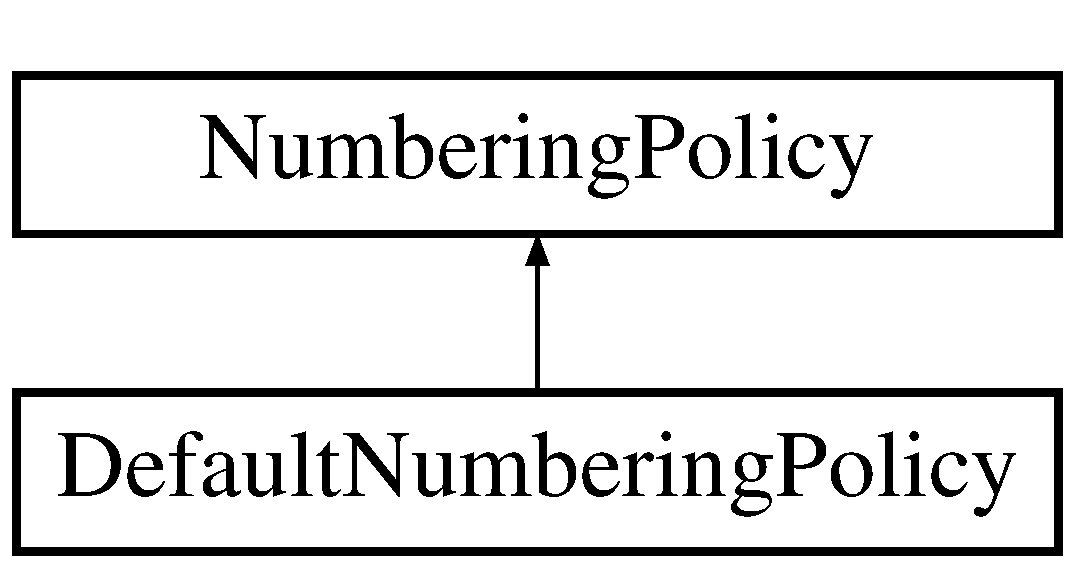
\includegraphics[height=2cm]{classDefaultNumberingPolicy}
\end{center}
\end{figure}
\subsection*{Public メソッド}
\begin{DoxyCompactItemize}
\item 
{\bf DefaultNumberingPolicy} ()
\item 
virtual {\bf $\sim$DefaultNumberingPolicy} (void)
\begin{DoxyCompactList}\small\item\em デストラクタ \item\end{DoxyCompactList}\item 
virtual std::string {\bf onCreate} (void $\ast$obj)
\begin{DoxyCompactList}\small\item\em オブジェクト生成時の名称作成 \item\end{DoxyCompactList}\item 
virtual void {\bf onDelete} (void $\ast$obj)
\begin{DoxyCompactList}\small\item\em オブジェクト削除時の名称解放 \item\end{DoxyCompactList}\end{DoxyCompactItemize}
\subsection*{Protected メソッド}
\begin{DoxyCompactItemize}
\item 
long int {\bf find} (void $\ast$obj)
\begin{DoxyCompactList}\small\item\em オブジェクトの検索 \item\end{DoxyCompactList}\end{DoxyCompactItemize}


\subsection{説明}
オブジェクト生成時ネーミング・ポリシー(命名規則)管理用クラス オブジェクトを生成する際のネーミング・ポリシー(命名規則)を管理するための クラス。

\begin{DoxySince}{から}
0.4.0 
\end{DoxySince}


\subsection{コンストラクタとデストラクタ}
\index{DefaultNumberingPolicy@{DefaultNumberingPolicy}!DefaultNumberingPolicy@{DefaultNumberingPolicy}}
\index{DefaultNumberingPolicy@{DefaultNumberingPolicy}!DefaultNumberingPolicy@{DefaultNumberingPolicy}}
\subsubsection[{DefaultNumberingPolicy}]{\setlength{\rightskip}{0pt plus 5cm}DefaultNumberingPolicy::DefaultNumberingPolicy ()\hspace{0.3cm}{\ttfamily  [inline]}}\label{classDefaultNumberingPolicy_a23d721393d786e7abb7cb08c1763c44a}
コンストラクタ \index{DefaultNumberingPolicy@{DefaultNumberingPolicy}!$\sim$DefaultNumberingPolicy@{$\sim$DefaultNumberingPolicy}}
\index{$\sim$DefaultNumberingPolicy@{$\sim$DefaultNumberingPolicy}!DefaultNumberingPolicy@{DefaultNumberingPolicy}}
\subsubsection[{$\sim$DefaultNumberingPolicy}]{\setlength{\rightskip}{0pt plus 5cm}virtual DefaultNumberingPolicy::$\sim$DefaultNumberingPolicy (void)\hspace{0.3cm}{\ttfamily  [inline, virtual]}}\label{classDefaultNumberingPolicy_aeb44191706cd96bd89968b969e8ea9b4}


デストラクタ 



\subsection{関数}
\index{DefaultNumberingPolicy@{DefaultNumberingPolicy}!find@{find}}
\index{find@{find}!DefaultNumberingPolicy@{DefaultNumberingPolicy}}
\subsubsection[{find}]{\setlength{\rightskip}{0pt plus 5cm}long int DefaultNumberingPolicy::find (void $\ast$ {\em obj})\hspace{0.3cm}{\ttfamily  [protected]}}\label{classDefaultNumberingPolicy_a1b8f6103327b51c80aeed0e1c0683797}


オブジェクトの検索 

オブジェクトリストから指定されたオブジェクトを検索し、 該当するオブジェクトが格納されている場合にはインデックスを返す。


\begin{DoxyParams}{引数}
\item[{\em obj}]検索対象オブジェクト\end{DoxyParams}
\begin{DoxyReturn}{戻り値}
オブジェクト格納インデックス 
\end{DoxyReturn}
\index{DefaultNumberingPolicy@{DefaultNumberingPolicy}!onCreate@{onCreate}}
\index{onCreate@{onCreate}!DefaultNumberingPolicy@{DefaultNumberingPolicy}}
\subsubsection[{onCreate}]{\setlength{\rightskip}{0pt plus 5cm}virtual std::string DefaultNumberingPolicy::onCreate (void $\ast$ {\em obj})\hspace{0.3cm}{\ttfamily  [virtual]}}\label{classDefaultNumberingPolicy_ad446abe9c24085dc3676a316e0d5da0c}


オブジェクト生成時の名称作成 

オブジェクト生成時の名称を生成する。 生成済みインスタンスの数に応じた名称を生成する。


\begin{DoxyParams}{引数}
\item[{\em obj}]名称生成対象オブジェクト\end{DoxyParams}
\begin{DoxyReturn}{戻り値}
生成したオブジェクト名称 
\end{DoxyReturn}


{\bf NumberingPolicy} \doxyref{}{p.}{classNumberingPolicy_a5a24d7cdf2cff8c97b1c798114504c31}を実装しています。

\index{DefaultNumberingPolicy@{DefaultNumberingPolicy}!onDelete@{onDelete}}
\index{onDelete@{onDelete}!DefaultNumberingPolicy@{DefaultNumberingPolicy}}
\subsubsection[{onDelete}]{\setlength{\rightskip}{0pt plus 5cm}virtual void DefaultNumberingPolicy::onDelete (void $\ast$ {\em obj})\hspace{0.3cm}{\ttfamily  [virtual]}}\label{classDefaultNumberingPolicy_a216be8d1b29ecf328f04f98516364182}


オブジェクト削除時の名称解放 

オブジェクト削除時に名称を解放する。 オブジェクト削除時に生成済みインスタンス数を減算する。


\begin{DoxyParams}{引数}
\item[{\em obj}]名称解放対象オブジェクト \end{DoxyParams}


{\bf NumberingPolicy} \doxyref{}{p.}{classNumberingPolicy_a0bc5ddc2193e6415142327b4a5814d86}を実装しています。


\section{クラス テンプレート RTC::PeriodicExecutionContext::DFP$<$ Object $>$}
\label{classRTC_1_1PeriodicExecutionContext_1_1DFP}\index{RTC::PeriodicExecutionContext::DFP@{RTC::PeriodicExecutionContext::DFP}}


\doxyref{DFP}{p.}{classRTC_1_1PeriodicExecutionContext_1_1DFP} クラス.  




{\ttfamily \#include $<$PeriodicExecutionContext.h$>$}

RTC::PeriodicExecutionContext::DFP$<$ Object $>$に対する継承グラフ\begin{figure}[H]
\begin{center}
\leavevmode
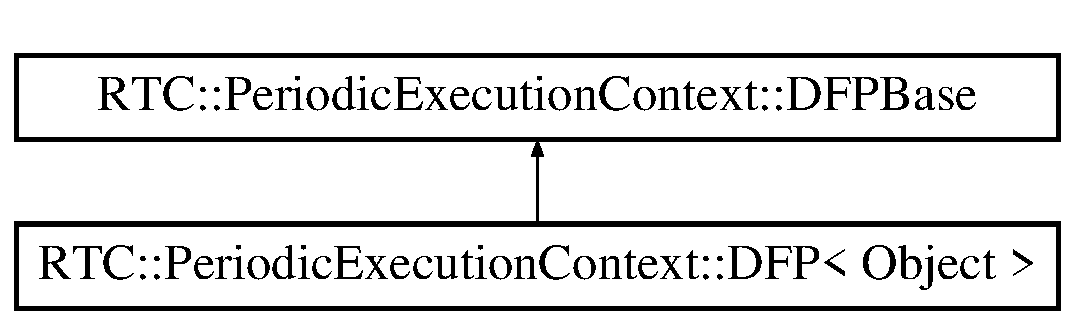
\includegraphics[height=2cm]{classRTC_1_1PeriodicExecutionContext_1_1DFP}
\end{center}
\end{figure}
\subsection*{Public メソッド}
\begin{DoxyCompactItemize}
\item 
{\bf DFP} (Object obj, ExecutionContextHandle\_\-t id)
\begin{DoxyCompactList}\small\item\em デフォルトコンストラクタ \item\end{DoxyCompactList}\item 
void {\bf on\_\-startup} (void)
\begin{DoxyCompactList}\small\item\em ExecutionContext 実行開始時に呼ばれる関数. \item\end{DoxyCompactList}\item 
void {\bf on\_\-shutdown} (void)
\begin{DoxyCompactList}\small\item\em ExecutionContext 停止時に呼ばれる関数. \item\end{DoxyCompactList}\item 
void {\bf on\_\-activated} (const {\bf ECStates} \&st)
\begin{DoxyCompactList}\small\item\em RTコンポーネントがアクティブ化された時に呼ばれる関数. \item\end{DoxyCompactList}\item 
void {\bf on\_\-deactivated} (const {\bf ECStates} \&st)
\begin{DoxyCompactList}\small\item\em RTコンポーネントが非アクティブ化された時に呼ばれる関数. \item\end{DoxyCompactList}\item 
void {\bf on\_\-aborting} (const {\bf ECStates} \&st)
\begin{DoxyCompactList}\small\item\em RTコンポーネントでエラーが発生した時に呼ばれる関数. \item\end{DoxyCompactList}\item 
void {\bf on\_\-error} (const {\bf ECStates} \&st)
\begin{DoxyCompactList}\small\item\em RTコンポーネントがエラー状態の時に呼ばれる関数. \item\end{DoxyCompactList}\item 
void {\bf on\_\-reset} (const {\bf ECStates} \&st)
\begin{DoxyCompactList}\small\item\em RTコンポーネントをリセットする時に呼ばれる関数. \item\end{DoxyCompactList}\item 
void {\bf on\_\-execute} (const {\bf ECStates} \&st)
\begin{DoxyCompactList}\small\item\em RTコンポーネント実行時に定期的に呼ばれる関数. \item\end{DoxyCompactList}\item 
void {\bf on\_\-state\_\-update} (const {\bf ECStates} \&st)
\begin{DoxyCompactList}\small\item\em RTコンポーネント実行時に定期的に呼ばれる関数. \item\end{DoxyCompactList}\item 
void {\bf on\_\-rate\_\-changed} (void)
\begin{DoxyCompactList}\small\item\em ExecutionContext の実行周期変更時に呼ばれる関数. \item\end{DoxyCompactList}\end{DoxyCompactItemize}
\subsection*{Public 変数}
\begin{DoxyCompactItemize}
\item 
Object {\bf m\_\-obj}
\begin{DoxyCompactList}\small\item\em 管理対象コンポーネント \item\end{DoxyCompactList}\item 
bool {\bf m\_\-active}
\begin{DoxyCompactList}\small\item\em 管理対象コンポーネントの動作状態フラグ \item\end{DoxyCompactList}\end{DoxyCompactItemize}


\subsection{説明}
\subsubsection*{template$<$class Object$>$ class RTC::PeriodicExecutionContext::DFP$<$ Object $>$}

\doxyref{DFP}{p.}{classRTC_1_1PeriodicExecutionContext_1_1DFP} クラス. 参加者リストに登録された DataFlowParticipant の関数を起動するための テンプレートクラス。


\begin{DoxyParams}{引数}
\item[{\em Object}]管理対象コンポーネントの型\end{DoxyParams}
\begin{DoxySince}{から}
0.4.0 
\end{DoxySince}


\subsection{コンストラクタとデストラクタ}
\index{RTC::PeriodicExecutionContext::DFP@{RTC::PeriodicExecutionContext::DFP}!DFP@{DFP}}
\index{DFP@{DFP}!RTC::PeriodicExecutionContext::DFP@{RTC::PeriodicExecutionContext::DFP}}
\subsubsection[{DFP}]{\setlength{\rightskip}{0pt plus 5cm}template$<$class Object$>$ {\bf RTC::PeriodicExecutionContext::DFP}$<$ Object $>$::{\bf DFP} (Object {\em obj}, \/  ExecutionContextHandle\_\-t {\em id})\hspace{0.3cm}{\ttfamily  [inline]}}\label{classRTC_1_1PeriodicExecutionContext_1_1DFP_a3a9221720e97918631cb49268e16058b}


デフォルトコンストラクタ 

デフォルトコンストラクタ


\begin{DoxyParams}{引数}
\item[{\em obj}]管理対象コンポーネント \item[{\em id}]所属する ExecutionContext のID \end{DoxyParams}


\subsection{関数}
\index{RTC::PeriodicExecutionContext::DFP@{RTC::PeriodicExecutionContext::DFP}!on\_\-aborting@{on\_\-aborting}}
\index{on\_\-aborting@{on\_\-aborting}!RTC::PeriodicExecutionContext::DFP@{RTC::PeriodicExecutionContext::DFP}}
\subsubsection[{on\_\-aborting}]{\setlength{\rightskip}{0pt plus 5cm}template$<$class Object$>$ void {\bf RTC::PeriodicExecutionContext::DFP}$<$ Object $>$::on\_\-aborting (const {\bf ECStates} \& {\em st})\hspace{0.3cm}{\ttfamily  [inline, virtual]}}\label{classRTC_1_1PeriodicExecutionContext_1_1DFP_a56b2f4893a7fd424fc744892581057d7}


RTコンポーネントでエラーが発生した時に呼ばれる関数. 

管理対象のRTコンポーネントにエラーが発生した時(Error状態へ遷移時) に管理対象コンポーネントの on\_\-aborting を呼びだす。


\begin{DoxyParams}{引数}
\item[{\em st}]対象RTコンポーネントの現在の状態 \end{DoxyParams}


{\bf RTC::PeriodicExecutionContext::DFPBase} \doxyref{}{p.}{classRTC_1_1PeriodicExecutionContext_1_1DFPBase_a4326e1e3a6fd23cd534c37016a9d6ff6}を実装しています。

\index{RTC::PeriodicExecutionContext::DFP@{RTC::PeriodicExecutionContext::DFP}!on\_\-activated@{on\_\-activated}}
\index{on\_\-activated@{on\_\-activated}!RTC::PeriodicExecutionContext::DFP@{RTC::PeriodicExecutionContext::DFP}}
\subsubsection[{on\_\-activated}]{\setlength{\rightskip}{0pt plus 5cm}template$<$class Object$>$ void {\bf RTC::PeriodicExecutionContext::DFP}$<$ Object $>$::on\_\-activated (const {\bf ECStates} \& {\em st})\hspace{0.3cm}{\ttfamily  [inline, virtual]}}\label{classRTC_1_1PeriodicExecutionContext_1_1DFP_aab354f4aec81a3de94c897d42a08814c}


RTコンポーネントがアクティブ化された時に呼ばれる関数. 

管理対象のRTコンポーネントがアクティブ化された時(Active状態へ遷移時) に、管理対象コンポーネントの on\_\-activated を呼びだす。 管理対象コンポーネントのアクティブ化が失敗した場合には、ステートマシン を Error 状態に遷移させる。


\begin{DoxyParams}{引数}
\item[{\em st}]対象RTコンポーネントの現在の状態 \end{DoxyParams}


{\bf RTC::PeriodicExecutionContext::DFPBase} \doxyref{}{p.}{classRTC_1_1PeriodicExecutionContext_1_1DFPBase_a7617ab4164f5516ee411a23273577148}を実装しています。

\index{RTC::PeriodicExecutionContext::DFP@{RTC::PeriodicExecutionContext::DFP}!on\_\-deactivated@{on\_\-deactivated}}
\index{on\_\-deactivated@{on\_\-deactivated}!RTC::PeriodicExecutionContext::DFP@{RTC::PeriodicExecutionContext::DFP}}
\subsubsection[{on\_\-deactivated}]{\setlength{\rightskip}{0pt plus 5cm}template$<$class Object$>$ void {\bf RTC::PeriodicExecutionContext::DFP}$<$ Object $>$::on\_\-deactivated (const {\bf ECStates} \& {\em st})\hspace{0.3cm}{\ttfamily  [inline, virtual]}}\label{classRTC_1_1PeriodicExecutionContext_1_1DFP_aa0b4398840866335bfd3a35aa2a1378c}


RTコンポーネントが非アクティブ化された時に呼ばれる関数. 

管理対象のRTコンポーネントが非アクティブ化された時 (Deactive状態へ遷移時)に、管理対象コンポーネントの on\_\-deactivated を 呼びだす。


\begin{DoxyParams}{引数}
\item[{\em st}]対象RTコンポーネントの現在の状態 \end{DoxyParams}


{\bf RTC::PeriodicExecutionContext::DFPBase} \doxyref{}{p.}{classRTC_1_1PeriodicExecutionContext_1_1DFPBase_afdb8f5efa070e18e5aecf34e117c4916}を実装しています。

\index{RTC::PeriodicExecutionContext::DFP@{RTC::PeriodicExecutionContext::DFP}!on\_\-error@{on\_\-error}}
\index{on\_\-error@{on\_\-error}!RTC::PeriodicExecutionContext::DFP@{RTC::PeriodicExecutionContext::DFP}}
\subsubsection[{on\_\-error}]{\setlength{\rightskip}{0pt plus 5cm}template$<$class Object$>$ void {\bf RTC::PeriodicExecutionContext::DFP}$<$ Object $>$::on\_\-error (const {\bf ECStates} \& {\em st})\hspace{0.3cm}{\ttfamily  [inline, virtual]}}\label{classRTC_1_1PeriodicExecutionContext_1_1DFP_a1921bae9d427aa285566e15bd08e6500}


RTコンポーネントがエラー状態の時に呼ばれる関数. 

管理対象のRTコンポーネントがエラー状態にいる間、 管理対象コンポーネントの on\_\-aborting を定期的に呼びだす。


\begin{DoxyParams}{引数}
\item[{\em st}]対象RTコンポーネントの現在の状態 \end{DoxyParams}


{\bf RTC::PeriodicExecutionContext::DFPBase} \doxyref{}{p.}{classRTC_1_1PeriodicExecutionContext_1_1DFPBase_aabc82635a64722f77fa359a4f6308122}を実装しています。

\index{RTC::PeriodicExecutionContext::DFP@{RTC::PeriodicExecutionContext::DFP}!on\_\-execute@{on\_\-execute}}
\index{on\_\-execute@{on\_\-execute}!RTC::PeriodicExecutionContext::DFP@{RTC::PeriodicExecutionContext::DFP}}
\subsubsection[{on\_\-execute}]{\setlength{\rightskip}{0pt plus 5cm}template$<$class Object$>$ void {\bf RTC::PeriodicExecutionContext::DFP}$<$ Object $>$::on\_\-execute (const {\bf ECStates} \& {\em st})\hspace{0.3cm}{\ttfamily  [inline, virtual]}}\label{classRTC_1_1PeriodicExecutionContext_1_1DFP_ab44ccec81e068726d371929b0b955a25}


RTコンポーネント実行時に定期的に呼ばれる関数. 

管理対象のRTコンポーネントが Active 状態であるとともに、 ExecutionContext が Running 状態の場合に、設定された動作周期で 定期的に管理対象コンポーネントの on\_\-execute を呼びだす。関数の 実行に失敗した場合(返値が RTC\_\-OK 以外)、管理対象コンポーネント の状態を Error 状態に遷移させる。


\begin{DoxyParams}{引数}
\item[{\em st}]対象RTコンポーネントの現在の状態 \end{DoxyParams}


{\bf RTC::PeriodicExecutionContext::DFPBase} \doxyref{}{p.}{classRTC_1_1PeriodicExecutionContext_1_1DFPBase_a4ac335580091c6300144717ed1ed4555}を実装しています。

\index{RTC::PeriodicExecutionContext::DFP@{RTC::PeriodicExecutionContext::DFP}!on\_\-rate\_\-changed@{on\_\-rate\_\-changed}}
\index{on\_\-rate\_\-changed@{on\_\-rate\_\-changed}!RTC::PeriodicExecutionContext::DFP@{RTC::PeriodicExecutionContext::DFP}}
\subsubsection[{on\_\-rate\_\-changed}]{\setlength{\rightskip}{0pt plus 5cm}template$<$class Object$>$ void {\bf RTC::PeriodicExecutionContext::DFP}$<$ Object $>$::on\_\-rate\_\-changed (void)\hspace{0.3cm}{\ttfamily  [inline, virtual]}}\label{classRTC_1_1PeriodicExecutionContext_1_1DFP_a283b40d3a75a439b2a0ac4f7e2740736}


ExecutionContext の実行周期変更時に呼ばれる関数. 

参加している ExecutionContext の実行周期が変更となった場合に、 管理対象コンポーネントの on\_\-rate\_\-changed を呼びだす。 

{\bf RTC::PeriodicExecutionContext::DFPBase} \doxyref{}{p.}{classRTC_1_1PeriodicExecutionContext_1_1DFPBase_a72fe285405c24be95d14f8c73ed993be}を実装しています。



参照元 RTC::PeriodicExecutionContext::invoke\_\-on\_\-rate\_\-changed::operator()().

\index{RTC::PeriodicExecutionContext::DFP@{RTC::PeriodicExecutionContext::DFP}!on\_\-reset@{on\_\-reset}}
\index{on\_\-reset@{on\_\-reset}!RTC::PeriodicExecutionContext::DFP@{RTC::PeriodicExecutionContext::DFP}}
\subsubsection[{on\_\-reset}]{\setlength{\rightskip}{0pt plus 5cm}template$<$class Object$>$ void {\bf RTC::PeriodicExecutionContext::DFP}$<$ Object $>$::on\_\-reset (const {\bf ECStates} \& {\em st})\hspace{0.3cm}{\ttfamily  [inline, virtual]}}\label{classRTC_1_1PeriodicExecutionContext_1_1DFP_adeb73de058b07b0abc6570c3e639cc5b}


RTコンポーネントをリセットする時に呼ばれる関数. 

管理対象のRTコンポーネントをリセットする際に、管理対象コンポーネント の on\_\-reset を呼びだす。


\begin{DoxyParams}{引数}
\item[{\em st}]対象RTコンポーネントの現在の状態 \end{DoxyParams}


{\bf RTC::PeriodicExecutionContext::DFPBase} \doxyref{}{p.}{classRTC_1_1PeriodicExecutionContext_1_1DFPBase_ad26d3a6118ce1f2b97527af86a8bb14d}を実装しています。

\index{RTC::PeriodicExecutionContext::DFP@{RTC::PeriodicExecutionContext::DFP}!on\_\-shutdown@{on\_\-shutdown}}
\index{on\_\-shutdown@{on\_\-shutdown}!RTC::PeriodicExecutionContext::DFP@{RTC::PeriodicExecutionContext::DFP}}
\subsubsection[{on\_\-shutdown}]{\setlength{\rightskip}{0pt plus 5cm}template$<$class Object$>$ void {\bf RTC::PeriodicExecutionContext::DFP}$<$ Object $>$::on\_\-shutdown (void)\hspace{0.3cm}{\ttfamily  [inline, virtual]}}\label{classRTC_1_1PeriodicExecutionContext_1_1DFP_a312588691ba1da141cae496d74bb2b7f}


ExecutionContext 停止時に呼ばれる関数. 

参加している ExecutionContext が実行を停止する時(Stopped状態へ遷移時) に、管理対象コンポーネントの on\_\-shutdown を呼びだす。 

{\bf RTC::PeriodicExecutionContext::DFPBase} \doxyref{}{p.}{classRTC_1_1PeriodicExecutionContext_1_1DFPBase_a9acf5ba2d252539b0d853e5492177a1b}を実装しています。



参照元 RTC::PeriodicExecutionContext::invoke\_\-on\_\-shutdown::operator()().

\index{RTC::PeriodicExecutionContext::DFP@{RTC::PeriodicExecutionContext::DFP}!on\_\-startup@{on\_\-startup}}
\index{on\_\-startup@{on\_\-startup}!RTC::PeriodicExecutionContext::DFP@{RTC::PeriodicExecutionContext::DFP}}
\subsubsection[{on\_\-startup}]{\setlength{\rightskip}{0pt plus 5cm}template$<$class Object$>$ void {\bf RTC::PeriodicExecutionContext::DFP}$<$ Object $>$::on\_\-startup (void)\hspace{0.3cm}{\ttfamily  [inline, virtual]}}\label{classRTC_1_1PeriodicExecutionContext_1_1DFP_a79b7b4a99f8d2cd0dc407c1b326dcb85}


ExecutionContext 実行開始時に呼ばれる関数. 

参加している ExecutionContext が実行を開始する時(Running状態へ遷移時) に、管理対象コンポーネントの on\_\-startup を呼びだす。 

{\bf RTC::PeriodicExecutionContext::DFPBase} \doxyref{}{p.}{classRTC_1_1PeriodicExecutionContext_1_1DFPBase_a761ebe484557229fe21a6b6488567d2f}を実装しています。



参照元 RTC::PeriodicExecutionContext::invoke\_\-on\_\-startup::operator()().

\index{RTC::PeriodicExecutionContext::DFP@{RTC::PeriodicExecutionContext::DFP}!on\_\-state\_\-update@{on\_\-state\_\-update}}
\index{on\_\-state\_\-update@{on\_\-state\_\-update}!RTC::PeriodicExecutionContext::DFP@{RTC::PeriodicExecutionContext::DFP}}
\subsubsection[{on\_\-state\_\-update}]{\setlength{\rightskip}{0pt plus 5cm}template$<$class Object$>$ void {\bf RTC::PeriodicExecutionContext::DFP}$<$ Object $>$::on\_\-state\_\-update (const {\bf ECStates} \& {\em st})\hspace{0.3cm}{\ttfamily  [inline, virtual]}}\label{classRTC_1_1PeriodicExecutionContext_1_1DFP_a0689e39bbc51b091833c3cf5ef070297}


RTコンポーネント実行時に定期的に呼ばれる関数. 

管理対象のRTコンポーネントが Active 状態であるとともに、 ExecutionContext が Running 状態の場合に、設定された動作周期で 定期的に管理対象コンポーネントの on\_\-state\_\-update を呼びだす。 関数の実行に失敗した場合(返値が RTC\_\-OK 以外)、管理対象コンポー ネントの状態を Error 状態に遷移させる。


\begin{DoxyParams}{引数}
\item[{\em st}]対象RTコンポーネントの現在の状態 \end{DoxyParams}


{\bf RTC::PeriodicExecutionContext::DFPBase} \doxyref{}{p.}{classRTC_1_1PeriodicExecutionContext_1_1DFPBase_a840339510d7a4d0eef17f495638bbbc3}を実装しています。



\subsection{変数}
\index{RTC::PeriodicExecutionContext::DFP@{RTC::PeriodicExecutionContext::DFP}!m\_\-active@{m\_\-active}}
\index{m\_\-active@{m\_\-active}!RTC::PeriodicExecutionContext::DFP@{RTC::PeriodicExecutionContext::DFP}}
\subsubsection[{m\_\-active}]{\setlength{\rightskip}{0pt plus 5cm}template$<$class Object$>$ bool {\bf RTC::PeriodicExecutionContext::DFP}$<$ Object $>$::{\bf m\_\-active}}\label{classRTC_1_1PeriodicExecutionContext_1_1DFP_a26c3f482f8c0fc239af8b180aa8de4de}


管理対象コンポーネントの動作状態フラグ 

\index{RTC::PeriodicExecutionContext::DFP@{RTC::PeriodicExecutionContext::DFP}!m\_\-obj@{m\_\-obj}}
\index{m\_\-obj@{m\_\-obj}!RTC::PeriodicExecutionContext::DFP@{RTC::PeriodicExecutionContext::DFP}}
\subsubsection[{m\_\-obj}]{\setlength{\rightskip}{0pt plus 5cm}template$<$class Object$>$ Object {\bf RTC::PeriodicExecutionContext::DFP}$<$ Object $>$::{\bf m\_\-obj}}\label{classRTC_1_1PeriodicExecutionContext_1_1DFP_a12f00ab69fa3e68cb5b0ee83dbe010af}


管理対象コンポーネント 



参照元 RTC::PeriodicExecutionContext::DFP$<$ OpenRTM::DataFlowComponent\_\-var $>$::on\_\-aborting(), RTC::PeriodicExecutionContext::DFP$<$ OpenRTM::DataFlowComponent\_\-var $>$::on\_\-activated(), RTC::PeriodicExecutionContext::DFP$<$ OpenRTM::DataFlowComponent\_\-var $>$::on\_\-deactivated(), RTC::PeriodicExecutionContext::DFP$<$ OpenRTM::DataFlowComponent\_\-var $>$::on\_\-error(), RTC::PeriodicExecutionContext::DFP$<$ OpenRTM::DataFlowComponent\_\-var $>$::on\_\-execute(), RTC::PeriodicExecutionContext::DFP$<$ OpenRTM::DataFlowComponent\_\-var $>$::on\_\-rate\_\-changed(), RTC::PeriodicExecutionContext::DFP$<$ OpenRTM::DataFlowComponent\_\-var $>$::on\_\-reset(), RTC::PeriodicExecutionContext::DFP$<$ OpenRTM::DataFlowComponent\_\-var $>$::on\_\-shutdown(), RTC::PeriodicExecutionContext::DFP$<$ OpenRTM::DataFlowComponent\_\-var $>$::on\_\-startup(), RTC::PeriodicExecutionContext::DFP$<$ OpenRTM::DataFlowComponent\_\-var $>$::on\_\-state\_\-update(), と RTC::PeriodicExecutionContext::Comp::operator=().


\section{クラス RTC::PeriodicExecutionContext::DFPBase}
\label{classRTC_1_1PeriodicExecutionContext_1_1DFPBase}\index{RTC::PeriodicExecutionContext::DFPBase@{RTC::PeriodicExecutionContext::DFPBase}}


\doxyref{DFPBase}{p.}{classRTC_1_1PeriodicExecutionContext_1_1DFPBase} クラス.  




{\ttfamily \#include $<$PeriodicExecutionContext.h$>$}

RTC::PeriodicExecutionContext::DFPBaseに対する継承グラフ\begin{figure}[H]
\begin{center}
\leavevmode
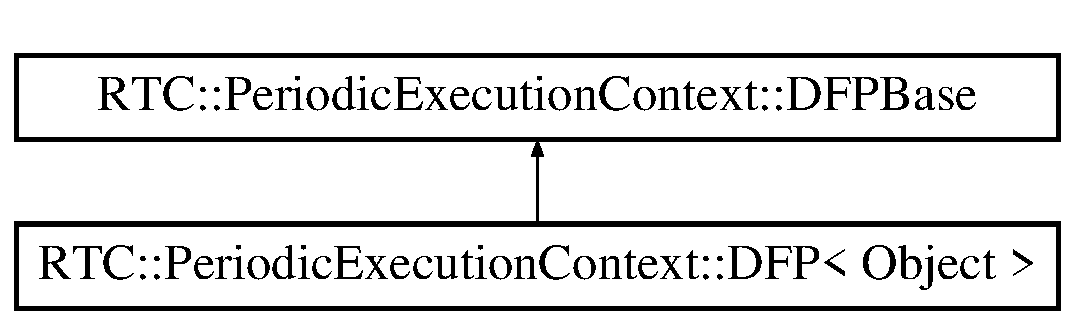
\includegraphics[height=2cm]{classRTC_1_1PeriodicExecutionContext_1_1DFPBase}
\end{center}
\end{figure}
\subsection*{Public メソッド}
\begin{DoxyCompactItemize}
\item 
{\bf DFPBase} (RTC::ExecutionContextHandle\_\-t id)
\begin{DoxyCompactList}\small\item\em コンストラクタ \item\end{DoxyCompactList}\item 
virtual {\bf $\sim$DFPBase} (void)
\item 
virtual void {\bf on\_\-startup} (void)=0
\begin{DoxyCompactList}\small\item\em ExecutionContext 実行開始時に呼ばれる純粋仮想関数. \item\end{DoxyCompactList}\item 
virtual void {\bf on\_\-shutdown} (void)=0
\begin{DoxyCompactList}\small\item\em ExecutionContext 停止時に呼ばれる純粋仮想関数. \item\end{DoxyCompactList}\item 
virtual void {\bf on\_\-activated} (const {\bf ECStates} \&st)=0
\begin{DoxyCompactList}\small\item\em RTコンポーネントがアクティブ化された時に呼ばれる純粋仮想関数. \item\end{DoxyCompactList}\item 
virtual void {\bf on\_\-deactivated} (const {\bf ECStates} \&st)=0
\begin{DoxyCompactList}\small\item\em RTコンポーネントが非アクティブ化された時に呼ばれる純粋仮想関数. \item\end{DoxyCompactList}\item 
virtual void {\bf on\_\-aborting} (const {\bf ECStates} \&st)=0
\begin{DoxyCompactList}\small\item\em RTコンポーネントでエラーが発生した時に呼ばれる純粋仮想関数. \item\end{DoxyCompactList}\item 
virtual void {\bf on\_\-error} (const {\bf ECStates} \&st)=0
\begin{DoxyCompactList}\small\item\em RTコンポーネントがエラー状態の時に呼ばれる純粋仮想関数. \item\end{DoxyCompactList}\item 
virtual void {\bf on\_\-reset} (const {\bf ECStates} \&st)=0
\begin{DoxyCompactList}\small\item\em RTコンポーネントをリセットする時に呼ばれる純粋仮想関数. \item\end{DoxyCompactList}\item 
virtual void {\bf on\_\-execute} (const {\bf ECStates} \&st)=0
\begin{DoxyCompactList}\small\item\em RTコンポーネント実行時に定期的に呼ばれる純粋仮想関数. \item\end{DoxyCompactList}\item 
virtual void {\bf on\_\-state\_\-update} (const {\bf ECStates} \&st)=0
\begin{DoxyCompactList}\small\item\em RTコンポーネント実行時に定期的に呼ばれる純粋仮想関数. \item\end{DoxyCompactList}\item 
virtual void {\bf on\_\-rate\_\-changed} (void)=0
\begin{DoxyCompactList}\small\item\em ExecutionContext の実行周期変更時に呼ばれる純粋仮想関数. \item\end{DoxyCompactList}\item 
virtual void {\bf worker} (void)
\begin{DoxyCompactList}\small\item\em 状態遷移を実行するワーカーを取得する \item\end{DoxyCompactList}\item 
virtual {\bf ExecContextState} {\bf get\_\-state} (void)
\begin{DoxyCompactList}\small\item\em 現在の状態を取得する \item\end{DoxyCompactList}\end{DoxyCompactItemize}
\subsection*{Public 変数}
\begin{DoxyCompactItemize}
\item 
ExecutionContextHandle\_\-t {\bf ec\_\-id}
\begin{DoxyCompactList}\small\item\em 参加している ExecutionContext の ID \item\end{DoxyCompactList}\item 
{\bf RTC\_\-Utils::StateMachine}$<$ {\bf ExecContextState}, {\bf DFPBase} $>$ {\bf m\_\-sm}
\begin{DoxyCompactList}\small\item\em 管理対象RTコンポーネントのステートマシン \item\end{DoxyCompactList}\end{DoxyCompactItemize}


\subsection{説明}
\doxyref{DFPBase}{p.}{classRTC_1_1PeriodicExecutionContext_1_1DFPBase} クラス. 参加者リストに登録された DataFlowParticipant を管理するための抽象クラス。

\begin{DoxySince}{から}
0.4.0 
\end{DoxySince}


\subsection{コンストラクタとデストラクタ}
\index{RTC::PeriodicExecutionContext::DFPBase@{RTC::PeriodicExecutionContext::DFPBase}!DFPBase@{DFPBase}}
\index{DFPBase@{DFPBase}!RTC::PeriodicExecutionContext::DFPBase@{RTC::PeriodicExecutionContext::DFPBase}}
\subsubsection[{DFPBase}]{\setlength{\rightskip}{0pt plus 5cm}RTC::PeriodicExecutionContext::DFPBase::DFPBase (RTC::ExecutionContextHandle\_\-t {\em id})\hspace{0.3cm}{\ttfamily  [inline]}}\label{classRTC_1_1PeriodicExecutionContext_1_1DFPBase_a3319f153362c46e858a0fdcc0f2568d8}


コンストラクタ 

コンストラクタ


\begin{DoxyParams}{引数}
\item[{\em id}]所属する ExecutionContext のID \end{DoxyParams}


参照先 RTC\_\-Utils::StateHolder$<$ State $>$::curr, RTC\_\-Utils::StateHolder$<$ State $>$::next, on\_\-aborting(), on\_\-activated(), on\_\-deactivated(), on\_\-error(), on\_\-execute(), on\_\-reset(), on\_\-state\_\-update(), と RTC\_\-Utils::StateHolder$<$ State $>$::prev.

\index{RTC::PeriodicExecutionContext::DFPBase@{RTC::PeriodicExecutionContext::DFPBase}!$\sim$DFPBase@{$\sim$DFPBase}}
\index{$\sim$DFPBase@{$\sim$DFPBase}!RTC::PeriodicExecutionContext::DFPBase@{RTC::PeriodicExecutionContext::DFPBase}}
\subsubsection[{$\sim$DFPBase}]{\setlength{\rightskip}{0pt plus 5cm}virtual RTC::PeriodicExecutionContext::DFPBase::$\sim$DFPBase (void)\hspace{0.3cm}{\ttfamily  [inline, virtual]}}\label{classRTC_1_1PeriodicExecutionContext_1_1DFPBase_a382e8b3d00a1e71244e8ef63989c631c}
デストラクタ 

\subsection{関数}
\index{RTC::PeriodicExecutionContext::DFPBase@{RTC::PeriodicExecutionContext::DFPBase}!get\_\-state@{get\_\-state}}
\index{get\_\-state@{get\_\-state}!RTC::PeriodicExecutionContext::DFPBase@{RTC::PeriodicExecutionContext::DFPBase}}
\subsubsection[{get\_\-state}]{\setlength{\rightskip}{0pt plus 5cm}virtual {\bf ExecContextState} RTC::PeriodicExecutionContext::DFPBase::get\_\-state (void)\hspace{0.3cm}{\ttfamily  [inline, virtual]}}\label{classRTC_1_1PeriodicExecutionContext_1_1DFPBase_a9cb860e561b642df7ae8dbfb089f71e1}


現在の状態を取得する 

管理対象RTコンポーネントの現在の状態を取得する。

\begin{DoxyReturn}{戻り値}
現在状態 
\end{DoxyReturn}
\index{RTC::PeriodicExecutionContext::DFPBase@{RTC::PeriodicExecutionContext::DFPBase}!on\_\-aborting@{on\_\-aborting}}
\index{on\_\-aborting@{on\_\-aborting}!RTC::PeriodicExecutionContext::DFPBase@{RTC::PeriodicExecutionContext::DFPBase}}
\subsubsection[{on\_\-aborting}]{\setlength{\rightskip}{0pt plus 5cm}virtual void RTC::PeriodicExecutionContext::DFPBase::on\_\-aborting (const {\bf ECStates} \& {\em st})\hspace{0.3cm}{\ttfamily  [pure virtual]}}\label{classRTC_1_1PeriodicExecutionContext_1_1DFPBase_a4326e1e3a6fd23cd534c37016a9d6ff6}


RTコンポーネントでエラーが発生した時に呼ばれる純粋仮想関数. 

管理対象のRTコンポーネントにエラーが発生した時(Error状態へ遷移時) に呼ばれる純粋仮想関数。


\begin{DoxyParams}{引数}
\item[{\em st}]対象RTコンポーネントの現在の状態 \end{DoxyParams}


{\bf RTC::PeriodicExecutionContext::DFP$<$ Object $>$} \doxyref{}{p.}{classRTC_1_1PeriodicExecutionContext_1_1DFP_a56b2f4893a7fd424fc744892581057d7}, と {\bf RTC::PeriodicExecutionContext::DFP$<$ OpenRTM::DataFlowComponent\_\-var $>$} \doxyref{}{p.}{classRTC_1_1PeriodicExecutionContext_1_1DFP_a56b2f4893a7fd424fc744892581057d7}で実装されています。



参照元 DFPBase().

\index{RTC::PeriodicExecutionContext::DFPBase@{RTC::PeriodicExecutionContext::DFPBase}!on\_\-activated@{on\_\-activated}}
\index{on\_\-activated@{on\_\-activated}!RTC::PeriodicExecutionContext::DFPBase@{RTC::PeriodicExecutionContext::DFPBase}}
\subsubsection[{on\_\-activated}]{\setlength{\rightskip}{0pt plus 5cm}virtual void RTC::PeriodicExecutionContext::DFPBase::on\_\-activated (const {\bf ECStates} \& {\em st})\hspace{0.3cm}{\ttfamily  [pure virtual]}}\label{classRTC_1_1PeriodicExecutionContext_1_1DFPBase_a7617ab4164f5516ee411a23273577148}


RTコンポーネントがアクティブ化された時に呼ばれる純粋仮想関数. 

管理対象のRTコンポーネントがアクティブ化された時 (Active状態へ遷移時)に呼ばれる純粋仮想関数。


\begin{DoxyParams}{引数}
\item[{\em st}]対象RTコンポーネントの現在の状態 \end{DoxyParams}


{\bf RTC::PeriodicExecutionContext::DFP$<$ Object $>$} \doxyref{}{p.}{classRTC_1_1PeriodicExecutionContext_1_1DFP_aab354f4aec81a3de94c897d42a08814c}, と {\bf RTC::PeriodicExecutionContext::DFP$<$ OpenRTM::DataFlowComponent\_\-var $>$} \doxyref{}{p.}{classRTC_1_1PeriodicExecutionContext_1_1DFP_aab354f4aec81a3de94c897d42a08814c}で実装されています。



参照元 DFPBase().

\index{RTC::PeriodicExecutionContext::DFPBase@{RTC::PeriodicExecutionContext::DFPBase}!on\_\-deactivated@{on\_\-deactivated}}
\index{on\_\-deactivated@{on\_\-deactivated}!RTC::PeriodicExecutionContext::DFPBase@{RTC::PeriodicExecutionContext::DFPBase}}
\subsubsection[{on\_\-deactivated}]{\setlength{\rightskip}{0pt plus 5cm}virtual void RTC::PeriodicExecutionContext::DFPBase::on\_\-deactivated (const {\bf ECStates} \& {\em st})\hspace{0.3cm}{\ttfamily  [pure virtual]}}\label{classRTC_1_1PeriodicExecutionContext_1_1DFPBase_afdb8f5efa070e18e5aecf34e117c4916}


RTコンポーネントが非アクティブ化された時に呼ばれる純粋仮想関数. 

管理対象のRTコンポーネントが非アクティブ化された時 (Deactive状態へ遷移時)に呼ばれる純粋仮想関数。


\begin{DoxyParams}{引数}
\item[{\em st}]対象RTコンポーネントの現在の状態 \end{DoxyParams}


{\bf RTC::PeriodicExecutionContext::DFP$<$ Object $>$} \doxyref{}{p.}{classRTC_1_1PeriodicExecutionContext_1_1DFP_aa0b4398840866335bfd3a35aa2a1378c}, と {\bf RTC::PeriodicExecutionContext::DFP$<$ OpenRTM::DataFlowComponent\_\-var $>$} \doxyref{}{p.}{classRTC_1_1PeriodicExecutionContext_1_1DFP_aa0b4398840866335bfd3a35aa2a1378c}で実装されています。



参照元 DFPBase().

\index{RTC::PeriodicExecutionContext::DFPBase@{RTC::PeriodicExecutionContext::DFPBase}!on\_\-error@{on\_\-error}}
\index{on\_\-error@{on\_\-error}!RTC::PeriodicExecutionContext::DFPBase@{RTC::PeriodicExecutionContext::DFPBase}}
\subsubsection[{on\_\-error}]{\setlength{\rightskip}{0pt plus 5cm}virtual void RTC::PeriodicExecutionContext::DFPBase::on\_\-error (const {\bf ECStates} \& {\em st})\hspace{0.3cm}{\ttfamily  [pure virtual]}}\label{classRTC_1_1PeriodicExecutionContext_1_1DFPBase_aabc82635a64722f77fa359a4f6308122}


RTコンポーネントがエラー状態の時に呼ばれる純粋仮想関数. 

管理対象のRTコンポーネントがエラー状態にいる間、on\_\-execute と on\_\-state\_\-update に替わって定期的に呼び出される純粋仮想関数。


\begin{DoxyParams}{引数}
\item[{\em st}]対象RTコンポーネントの現在の状態 \end{DoxyParams}


{\bf RTC::PeriodicExecutionContext::DFP$<$ Object $>$} \doxyref{}{p.}{classRTC_1_1PeriodicExecutionContext_1_1DFP_a1921bae9d427aa285566e15bd08e6500}, と {\bf RTC::PeriodicExecutionContext::DFP$<$ OpenRTM::DataFlowComponent\_\-var $>$} \doxyref{}{p.}{classRTC_1_1PeriodicExecutionContext_1_1DFP_a1921bae9d427aa285566e15bd08e6500}で実装されています。



参照元 DFPBase().

\index{RTC::PeriodicExecutionContext::DFPBase@{RTC::PeriodicExecutionContext::DFPBase}!on\_\-execute@{on\_\-execute}}
\index{on\_\-execute@{on\_\-execute}!RTC::PeriodicExecutionContext::DFPBase@{RTC::PeriodicExecutionContext::DFPBase}}
\subsubsection[{on\_\-execute}]{\setlength{\rightskip}{0pt plus 5cm}virtual void RTC::PeriodicExecutionContext::DFPBase::on\_\-execute (const {\bf ECStates} \& {\em st})\hspace{0.3cm}{\ttfamily  [pure virtual]}}\label{classRTC_1_1PeriodicExecutionContext_1_1DFPBase_a4ac335580091c6300144717ed1ed4555}


RTコンポーネント実行時に定期的に呼ばれる純粋仮想関数. 

管理対象のRTコンポーネントが Active 状態であるとともに、 ExecutionContext が Running 状態の場合に、設定された動作周期で定期的に 呼び出される純粋仮想関数。 Two-\/Pass Execution の最初の実行で呼ばれる。


\begin{DoxyParams}{引数}
\item[{\em st}]対象RTコンポーネントの現在の状態 \end{DoxyParams}


{\bf RTC::PeriodicExecutionContext::DFP$<$ Object $>$} \doxyref{}{p.}{classRTC_1_1PeriodicExecutionContext_1_1DFP_ab44ccec81e068726d371929b0b955a25}, と {\bf RTC::PeriodicExecutionContext::DFP$<$ OpenRTM::DataFlowComponent\_\-var $>$} \doxyref{}{p.}{classRTC_1_1PeriodicExecutionContext_1_1DFP_ab44ccec81e068726d371929b0b955a25}で実装されています。



参照元 DFPBase().

\index{RTC::PeriodicExecutionContext::DFPBase@{RTC::PeriodicExecutionContext::DFPBase}!on\_\-rate\_\-changed@{on\_\-rate\_\-changed}}
\index{on\_\-rate\_\-changed@{on\_\-rate\_\-changed}!RTC::PeriodicExecutionContext::DFPBase@{RTC::PeriodicExecutionContext::DFPBase}}
\subsubsection[{on\_\-rate\_\-changed}]{\setlength{\rightskip}{0pt plus 5cm}virtual void RTC::PeriodicExecutionContext::DFPBase::on\_\-rate\_\-changed (void)\hspace{0.3cm}{\ttfamily  [pure virtual]}}\label{classRTC_1_1PeriodicExecutionContext_1_1DFPBase_a72fe285405c24be95d14f8c73ed993be}


ExecutionContext の実行周期変更時に呼ばれる純粋仮想関数. 

参加している ExecutionContext の実行周期が変更となった場合に、 この変更を伝達するために呼び出される純粋仮想関数。 

{\bf RTC::PeriodicExecutionContext::DFP$<$ Object $>$} \doxyref{}{p.}{classRTC_1_1PeriodicExecutionContext_1_1DFP_a283b40d3a75a439b2a0ac4f7e2740736}, と {\bf RTC::PeriodicExecutionContext::DFP$<$ OpenRTM::DataFlowComponent\_\-var $>$} \doxyref{}{p.}{classRTC_1_1PeriodicExecutionContext_1_1DFP_a283b40d3a75a439b2a0ac4f7e2740736}で実装されています。

\index{RTC::PeriodicExecutionContext::DFPBase@{RTC::PeriodicExecutionContext::DFPBase}!on\_\-reset@{on\_\-reset}}
\index{on\_\-reset@{on\_\-reset}!RTC::PeriodicExecutionContext::DFPBase@{RTC::PeriodicExecutionContext::DFPBase}}
\subsubsection[{on\_\-reset}]{\setlength{\rightskip}{0pt plus 5cm}virtual void RTC::PeriodicExecutionContext::DFPBase::on\_\-reset (const {\bf ECStates} \& {\em st})\hspace{0.3cm}{\ttfamily  [pure virtual]}}\label{classRTC_1_1PeriodicExecutionContext_1_1DFPBase_ad26d3a6118ce1f2b97527af86a8bb14d}


RTコンポーネントをリセットする時に呼ばれる純粋仮想関数. 

管理対象のRTコンポーネントをリセットする際に呼ばれる純粋仮想関数。 この関数が正常に終了すると,RTCは Inactive 状態に復帰する。 この関数が正常に終了しなかった場合は, Error 状態に留まる。


\begin{DoxyParams}{引数}
\item[{\em st}]対象RTコンポーネントの現在の状態 \end{DoxyParams}


{\bf RTC::PeriodicExecutionContext::DFP$<$ Object $>$} \doxyref{}{p.}{classRTC_1_1PeriodicExecutionContext_1_1DFP_adeb73de058b07b0abc6570c3e639cc5b}, と {\bf RTC::PeriodicExecutionContext::DFP$<$ OpenRTM::DataFlowComponent\_\-var $>$} \doxyref{}{p.}{classRTC_1_1PeriodicExecutionContext_1_1DFP_adeb73de058b07b0abc6570c3e639cc5b}で実装されています。



参照元 DFPBase().

\index{RTC::PeriodicExecutionContext::DFPBase@{RTC::PeriodicExecutionContext::DFPBase}!on\_\-shutdown@{on\_\-shutdown}}
\index{on\_\-shutdown@{on\_\-shutdown}!RTC::PeriodicExecutionContext::DFPBase@{RTC::PeriodicExecutionContext::DFPBase}}
\subsubsection[{on\_\-shutdown}]{\setlength{\rightskip}{0pt plus 5cm}virtual void RTC::PeriodicExecutionContext::DFPBase::on\_\-shutdown (void)\hspace{0.3cm}{\ttfamily  [pure virtual]}}\label{classRTC_1_1PeriodicExecutionContext_1_1DFPBase_a9acf5ba2d252539b0d853e5492177a1b}


ExecutionContext 停止時に呼ばれる純粋仮想関数. 

参加している ExecutionContext が実行を停止する時(Stopped状態へ遷移時) に呼ばれる純粋仮想関数。 

{\bf RTC::PeriodicExecutionContext::DFP$<$ Object $>$} \doxyref{}{p.}{classRTC_1_1PeriodicExecutionContext_1_1DFP_a312588691ba1da141cae496d74bb2b7f}, と {\bf RTC::PeriodicExecutionContext::DFP$<$ OpenRTM::DataFlowComponent\_\-var $>$} \doxyref{}{p.}{classRTC_1_1PeriodicExecutionContext_1_1DFP_a312588691ba1da141cae496d74bb2b7f}で実装されています。

\index{RTC::PeriodicExecutionContext::DFPBase@{RTC::PeriodicExecutionContext::DFPBase}!on\_\-startup@{on\_\-startup}}
\index{on\_\-startup@{on\_\-startup}!RTC::PeriodicExecutionContext::DFPBase@{RTC::PeriodicExecutionContext::DFPBase}}
\subsubsection[{on\_\-startup}]{\setlength{\rightskip}{0pt plus 5cm}virtual void RTC::PeriodicExecutionContext::DFPBase::on\_\-startup (void)\hspace{0.3cm}{\ttfamily  [pure virtual]}}\label{classRTC_1_1PeriodicExecutionContext_1_1DFPBase_a761ebe484557229fe21a6b6488567d2f}


ExecutionContext 実行開始時に呼ばれる純粋仮想関数. 

参加している ExecutionContext が実行を開始する時(Running状態へ遷移時) に呼ばれる純粋仮想関数。 

{\bf RTC::PeriodicExecutionContext::DFP$<$ Object $>$} \doxyref{}{p.}{classRTC_1_1PeriodicExecutionContext_1_1DFP_a79b7b4a99f8d2cd0dc407c1b326dcb85}, と {\bf RTC::PeriodicExecutionContext::DFP$<$ OpenRTM::DataFlowComponent\_\-var $>$} \doxyref{}{p.}{classRTC_1_1PeriodicExecutionContext_1_1DFP_a79b7b4a99f8d2cd0dc407c1b326dcb85}で実装されています。

\index{RTC::PeriodicExecutionContext::DFPBase@{RTC::PeriodicExecutionContext::DFPBase}!on\_\-state\_\-update@{on\_\-state\_\-update}}
\index{on\_\-state\_\-update@{on\_\-state\_\-update}!RTC::PeriodicExecutionContext::DFPBase@{RTC::PeriodicExecutionContext::DFPBase}}
\subsubsection[{on\_\-state\_\-update}]{\setlength{\rightskip}{0pt plus 5cm}virtual void RTC::PeriodicExecutionContext::DFPBase::on\_\-state\_\-update (const {\bf ECStates} \& {\em st})\hspace{0.3cm}{\ttfamily  [pure virtual]}}\label{classRTC_1_1PeriodicExecutionContext_1_1DFPBase_a840339510d7a4d0eef17f495638bbbc3}


RTコンポーネント実行時に定期的に呼ばれる純粋仮想関数. 

管理対象のRTコンポーネントが Active 状態であるとともに、 ExecutionContext が Running 状態の場合に、設定された動作周期で定期的に 呼び出される純粋仮想関数。 Two-\/Pass Execution の2番目の実行で呼ばれる。


\begin{DoxyParams}{引数}
\item[{\em st}]対象RTコンポーネントの現在の状態 \end{DoxyParams}


{\bf RTC::PeriodicExecutionContext::DFP$<$ Object $>$} \doxyref{}{p.}{classRTC_1_1PeriodicExecutionContext_1_1DFP_a0689e39bbc51b091833c3cf5ef070297}, と {\bf RTC::PeriodicExecutionContext::DFP$<$ OpenRTM::DataFlowComponent\_\-var $>$} \doxyref{}{p.}{classRTC_1_1PeriodicExecutionContext_1_1DFP_a0689e39bbc51b091833c3cf5ef070297}で実装されています。



参照元 DFPBase().

\index{RTC::PeriodicExecutionContext::DFPBase@{RTC::PeriodicExecutionContext::DFPBase}!worker@{worker}}
\index{worker@{worker}!RTC::PeriodicExecutionContext::DFPBase@{RTC::PeriodicExecutionContext::DFPBase}}
\subsubsection[{worker}]{\setlength{\rightskip}{0pt plus 5cm}virtual void RTC::PeriodicExecutionContext::DFPBase::worker (void)\hspace{0.3cm}{\ttfamily  [inline, virtual]}}\label{classRTC_1_1PeriodicExecutionContext_1_1DFPBase_a1b1091320b7e68b0e20ccca6ac506534}


状態遷移を実行するワーカーを取得する 

管理対象RTコンポーネントの状態遷移を実行するワーカーを取得する。

\begin{DoxyReturn}{戻り値}
ワーカー 
\end{DoxyReturn}


参照元 RTC::PeriodicExecutionContext::invoke\_\-worker::operator()().



\subsection{変数}
\index{RTC::PeriodicExecutionContext::DFPBase@{RTC::PeriodicExecutionContext::DFPBase}!ec\_\-id@{ec\_\-id}}
\index{ec\_\-id@{ec\_\-id}!RTC::PeriodicExecutionContext::DFPBase@{RTC::PeriodicExecutionContext::DFPBase}}
\subsubsection[{ec\_\-id}]{\setlength{\rightskip}{0pt plus 5cm}ExecutionContextHandle\_\-t {\bf RTC::PeriodicExecutionContext::DFPBase::ec\_\-id}}\label{classRTC_1_1PeriodicExecutionContext_1_1DFPBase_ac3e8abc57e496192d6291cc260901054}


参加している ExecutionContext の ID 



参照元 RTC::PeriodicExecutionContext::DFP$<$ OpenRTM::DataFlowComponent\_\-var $>$::on\_\-aborting(), RTC::PeriodicExecutionContext::DFP$<$ OpenRTM::DataFlowComponent\_\-var $>$::on\_\-activated(), RTC::PeriodicExecutionContext::DFP$<$ OpenRTM::DataFlowComponent\_\-var $>$::on\_\-deactivated(), RTC::PeriodicExecutionContext::DFP$<$ OpenRTM::DataFlowComponent\_\-var $>$::on\_\-error(), RTC::PeriodicExecutionContext::DFP$<$ OpenRTM::DataFlowComponent\_\-var $>$::on\_\-execute(), RTC::PeriodicExecutionContext::DFP$<$ OpenRTM::DataFlowComponent\_\-var $>$::on\_\-rate\_\-changed(), RTC::PeriodicExecutionContext::DFP$<$ OpenRTM::DataFlowComponent\_\-var $>$::on\_\-reset(), RTC::PeriodicExecutionContext::DFP$<$ OpenRTM::DataFlowComponent\_\-var $>$::on\_\-shutdown(), RTC::PeriodicExecutionContext::DFP$<$ OpenRTM::DataFlowComponent\_\-var $>$::on\_\-startup(), RTC::PeriodicExecutionContext::DFP$<$ OpenRTM::DataFlowComponent\_\-var $>$::on\_\-state\_\-update(), と RTC::PeriodicExecutionContext::Comp::operator=().

\index{RTC::PeriodicExecutionContext::DFPBase@{RTC::PeriodicExecutionContext::DFPBase}!m\_\-sm@{m\_\-sm}}
\index{m\_\-sm@{m\_\-sm}!RTC::PeriodicExecutionContext::DFPBase@{RTC::PeriodicExecutionContext::DFPBase}}
\subsubsection[{m\_\-sm}]{\setlength{\rightskip}{0pt plus 5cm}{\bf RTC\_\-Utils::StateMachine}$<${\bf ExecContextState}, {\bf DFPBase}$>$ {\bf RTC::PeriodicExecutionContext::DFPBase::m\_\-sm}}\label{classRTC_1_1PeriodicExecutionContext_1_1DFPBase_a0efcdc041f9f01491579acd729653a50}


管理対象RTコンポーネントのステートマシン 



参照元 RTC::PeriodicExecutionContext::DFP$<$ OpenRTM::DataFlowComponent\_\-var $>$::on\_\-activated(), RTC::PeriodicExecutionContext::DFP$<$ OpenRTM::DataFlowComponent\_\-var $>$::on\_\-execute(), RTC::PeriodicExecutionContext::DFP$<$ OpenRTM::DataFlowComponent\_\-var $>$::on\_\-reset(), と RTC::PeriodicExecutionContext::DFP$<$ OpenRTM::DataFlowComponent\_\-var $>$::on\_\-state\_\-update().


\section{RTC::DisconnectCallback Class Reference}
\label{classRTC_1_1DisconnectCallback}\index{RTC::DisconnectCallback@{RTC::DisconnectCallback}}


Callback functor abstract for disconnect/notify\_\-disconnect() funcs.  




{\ttfamily \#include $<$PortCallback.h$>$}

\subsection*{Public Member Functions}
\begin{DoxyCompactItemize}
\item 
virtual {\bf $\sim$DisconnectCallback} (void)
\begin{DoxyCompactList}\small\item\em Destructor. \item\end{DoxyCompactList}\item 
virtual void {\bf operator()} (const char $\ast$connector\_\-id)=0
\begin{DoxyCompactList}\small\item\em Callback method. \item\end{DoxyCompactList}\end{DoxyCompactItemize}


\subsection{Detailed Description}
Callback functor abstract for disconnect/notify\_\-disconnect() funcs. This is the interface for callback functor for disconnect/notify\_\-disconnect() invocation in Port. Argument is connector ID is given these functions.


\begin{DoxyParams}{Parameters}
\item[{\em connector\_\-id}]Connector ID\end{DoxyParams}
\begin{DoxySince}{Since}
1.0.0 
\end{DoxySince}


\subsection{Constructor \& Destructor Documentation}
\index{RTC::DisconnectCallback@{RTC::DisconnectCallback}!$\sim$DisconnectCallback@{$\sim$DisconnectCallback}}
\index{$\sim$DisconnectCallback@{$\sim$DisconnectCallback}!RTC::DisconnectCallback@{RTC::DisconnectCallback}}
\subsubsection[{$\sim$DisconnectCallback}]{\setlength{\rightskip}{0pt plus 5cm}virtual RTC::DisconnectCallback::$\sim$DisconnectCallback (void)\hspace{0.3cm}{\ttfamily  [inline, virtual]}}\label{classRTC_1_1DisconnectCallback_aee020344969e3996b91d6bf3873c9aab}


Destructor. 

Destructor 

\subsection{Member Function Documentation}
\index{RTC::DisconnectCallback@{RTC::DisconnectCallback}!operator()@{operator()}}
\index{operator()@{operator()}!RTC::DisconnectCallback@{RTC::DisconnectCallback}}
\subsubsection[{operator()}]{\setlength{\rightskip}{0pt plus 5cm}virtual void RTC::DisconnectCallback::operator() (const char $\ast$ {\em connector\_\-id})\hspace{0.3cm}{\ttfamily  [pure virtual]}}\label{classRTC_1_1DisconnectCallback_a2b4b524ad261d6da63e6649434015dab}


Callback method. 

This is the callback method invoked when disconnect/notify\_\-disconnect() invocation in Port.


\begin{DoxyParams}{Parameters}
\item[{\em connector\_\-id}]Connector ID \end{DoxyParams}

\section{構造体 RTC::ModuleManager::DLLEntity}
\label{structRTC_1_1ModuleManager_1_1DLLEntity}\index{RTC::ModuleManager::DLLEntity@{RTC::ModuleManager::DLLEntity}}


DLL管理用構造体.  




{\ttfamily \#include $<$ModuleManager.h$>$}

\subsection*{Public 変数}
\begin{DoxyCompactItemize}
\item 
{\bf coil::Properties} {\bf properties}
\item 
{\bf coil::DynamicLib} {\bf dll}
\end{DoxyCompactItemize}


\subsection{説明}
DLL管理用構造体. 

\subsection{変数}
\index{RTC::ModuleManager::DLLEntity@{RTC::ModuleManager::DLLEntity}!dll@{dll}}
\index{dll@{dll}!RTC::ModuleManager::DLLEntity@{RTC::ModuleManager::DLLEntity}}
\subsubsection[{dll}]{\setlength{\rightskip}{0pt plus 5cm}{\bf coil::DynamicLib} {\bf RTC::ModuleManager::DLLEntity::dll}}\label{structRTC_1_1ModuleManager_1_1DLLEntity_afe210678e87af07ccd3d5e46d5bfaa39}


参照元 RTC::ModuleManager::UnloadPred::operator()().

\index{RTC::ModuleManager::DLLEntity@{RTC::ModuleManager::DLLEntity}!properties@{properties}}
\index{properties@{properties}!RTC::ModuleManager::DLLEntity@{RTC::ModuleManager::DLLEntity}}
\subsubsection[{properties}]{\setlength{\rightskip}{0pt plus 5cm}{\bf coil::Properties} {\bf RTC::ModuleManager::DLLEntity::properties}}\label{structRTC_1_1ModuleManager_1_1DLLEntity_a9e03f69e5fef19e24e6eeaa4a4a45835}


参照元 RTC::ModuleManager::DllPred::operator()().


\section{RTC::ModuleManager::DllPred Class Reference}
\label{classRTC_1_1ModuleManager_1_1DllPred}\index{RTC::ModuleManager::DllPred@{RTC::ModuleManager::DllPred}}


Module list that has already loaded.  




{\ttfamily \#include $<$ModuleManager.h$>$}

\subsection*{Public Member Functions}
\begin{DoxyCompactItemize}
\item 
{\bf DllPred} (const char $\ast$filepath)
\item 
{\bf DllPred} (const {\bf DLLEntity} $\ast$dll)
\item 
bool {\bf operator()} ({\bf DLLEntity} $\ast$dllentity)
\end{DoxyCompactItemize}


\subsection{Detailed Description}
Module list that has already loaded. 

\subsection{Constructor \& Destructor Documentation}
\index{RTC::ModuleManager::DllPred@{RTC::ModuleManager::DllPred}!DllPred@{DllPred}}
\index{DllPred@{DllPred}!RTC::ModuleManager::DllPred@{RTC::ModuleManager::DllPred}}
\subsubsection[{DllPred}]{\setlength{\rightskip}{0pt plus 5cm}RTC::ModuleManager::DllPred::DllPred (const char $\ast$ {\em filepath})\hspace{0.3cm}{\ttfamily  [inline]}}\label{classRTC_1_1ModuleManager_1_1DllPred_a310047395705ffd885d7248607dadeba}
\index{RTC::ModuleManager::DllPred@{RTC::ModuleManager::DllPred}!DllPred@{DllPred}}
\index{DllPred@{DllPred}!RTC::ModuleManager::DllPred@{RTC::ModuleManager::DllPred}}
\subsubsection[{DllPred}]{\setlength{\rightskip}{0pt plus 5cm}RTC::ModuleManager::DllPred::DllPred (const {\bf DLLEntity} $\ast$ {\em dll})\hspace{0.3cm}{\ttfamily  [inline]}}\label{classRTC_1_1ModuleManager_1_1DllPred_a33b22d69fa04dbeafe0b8b8e207b59aa}


\subsection{Member Function Documentation}
\index{RTC::ModuleManager::DllPred@{RTC::ModuleManager::DllPred}!operator()@{operator()}}
\index{operator()@{operator()}!RTC::ModuleManager::DllPred@{RTC::ModuleManager::DllPred}}
\subsubsection[{operator()}]{\setlength{\rightskip}{0pt plus 5cm}bool RTC::ModuleManager::DllPred::operator() ({\bf DLLEntity} $\ast$ {\em dllentity})\hspace{0.3cm}{\ttfamily  [inline]}}\label{classRTC_1_1ModuleManager_1_1DllPred_a8f4c3819da12b3a7b4ea1c6c566c4c92}


References coil::Properties::getProperty(), and RTC::ModuleManager::DLLEntity::properties.


\section{coil::DynamicLib Class Reference}
\label{classcoil_1_1DynamicLib}\index{coil::DynamicLib@{coil::DynamicLib}}


\doxyref{DynamicLib}{p.}{classcoil_1_1DynamicLib} class.  




{\ttfamily \#include $<$DynamicLib.h$>$}

\subsection*{Public Member Functions}
\begin{DoxyCompactItemize}
\item 
{\bf DynamicLib} (int close\_\-handle\_\-on\_\-destruction=1)
\begin{DoxyCompactList}\small\item\em Constructor. \item\end{DoxyCompactList}\item 
{\bf DynamicLib} (const char $\ast$dynlib\_\-name, int open\_\-mode=COIL\_\-DEFAULT\_\-DYNLIB\_\-MODE, int close\_\-handle\_\-on\_\-destruction=1)
\begin{DoxyCompactList}\small\item\em Constructor. \item\end{DoxyCompactList}\item 
virtual {\bf $\sim$DynamicLib} ()
\begin{DoxyCompactList}\small\item\em Destructor. \item\end{DoxyCompactList}\item 
{\bf DynamicLib} (const {\bf DynamicLib} \&rhs)
\begin{DoxyCompactList}\small\item\em Copy Constructor. \item\end{DoxyCompactList}\item 
{\bf DynamicLib} \& {\bf operator=} (const {\bf DynamicLib} \&rhs)
\begin{DoxyCompactList}\small\item\em Assignment operator. \item\end{DoxyCompactList}\item 
virtual int {\bf open} (const char $\ast$dll\_\-name, int open\_\-mode=COIL\_\-DEFAULT\_\-DYNLIB\_\-MODE, int close\_\-handle\_\-on\_\-destruction=1)
\begin{DoxyCompactList}\small\item\em Load of the Dynamic link library. \item\end{DoxyCompactList}\item 
virtual int {\bf close} (void)
\begin{DoxyCompactList}\small\item\em Unload of the Dynamic link library. \item\end{DoxyCompactList}\item 
void $\ast$ {\bf symbol} (const char $\ast$symbol\_\-name)
\begin{DoxyCompactList}\small\item\em Return an address of the memory where a symbol was loaded. \item\end{DoxyCompactList}\item 
const char $\ast$ {\bf error} (void) const 
\begin{DoxyCompactList}\small\item\em Return the explanation message about the error. \item\end{DoxyCompactList}\end{DoxyCompactItemize}
\subsection*{Static Public Member Functions}
\begin{DoxyCompactItemize}
\item 
static int {\bf ForExternTest} (void)
\begin{DoxyCompactList}\small\item\em Unit Test. \item\end{DoxyCompactList}\end{DoxyCompactItemize}


\subsection{Detailed Description}
\doxyref{DynamicLib}{p.}{classcoil_1_1DynamicLib} class. 

\subsection{Constructor \& Destructor Documentation}
\index{coil::DynamicLib@{coil::DynamicLib}!DynamicLib@{DynamicLib}}
\index{DynamicLib@{DynamicLib}!coil::DynamicLib@{coil::DynamicLib}}
\subsubsection[{DynamicLib}]{\setlength{\rightskip}{0pt plus 5cm}coil::DynamicLib::DynamicLib (int {\em close\_\-handle\_\-on\_\-destruction} = {\ttfamily 1})}\label{classcoil_1_1DynamicLib_ad3bf31b617e31af37f210c4544e3241d}


Constructor. 

Constructor


\begin{DoxyParams}{Parameters}
\item[{\em close\_\-handle\_\-on\_\-destruction}]Close flag. \end{DoxyParams}
\index{coil::DynamicLib@{coil::DynamicLib}!DynamicLib@{DynamicLib}}
\index{DynamicLib@{DynamicLib}!coil::DynamicLib@{coil::DynamicLib}}
\subsubsection[{DynamicLib}]{\setlength{\rightskip}{0pt plus 5cm}coil::DynamicLib::DynamicLib (const char $\ast$ {\em dynlib\_\-name}, \/  int {\em open\_\-mode} = {\ttfamily COIL\_\-DEFAULT\_\-DYNLIB\_\-MODE}, \/  int {\em close\_\-handle\_\-on\_\-destruction} = {\ttfamily 1})}\label{classcoil_1_1DynamicLib_a212c930320798b941f496df140225922}


Constructor. 

Constructor


\begin{DoxyParams}{Parameters}
\item[{\em dynlib\_\-name}]Dynamic link library name. \item[{\em open\_\-mode}]Open mode. \item[{\em close\_\-handle\_\-on\_\-destruction}]Close flag. \end{DoxyParams}
\index{coil::DynamicLib@{coil::DynamicLib}!$\sim$DynamicLib@{$\sim$DynamicLib}}
\index{$\sim$DynamicLib@{$\sim$DynamicLib}!coil::DynamicLib@{coil::DynamicLib}}
\subsubsection[{$\sim$DynamicLib}]{\setlength{\rightskip}{0pt plus 5cm}virtual coil::DynamicLib::$\sim$DynamicLib ()\hspace{0.3cm}{\ttfamily  [virtual]}}\label{classcoil_1_1DynamicLib_a6b18812576274720376677384301c727}


Destructor. 

Destructor \index{coil::DynamicLib@{coil::DynamicLib}!DynamicLib@{DynamicLib}}
\index{DynamicLib@{DynamicLib}!coil::DynamicLib@{coil::DynamicLib}}
\subsubsection[{DynamicLib}]{\setlength{\rightskip}{0pt plus 5cm}coil::DynamicLib::DynamicLib (const {\bf DynamicLib} \& {\em rhs})}\label{classcoil_1_1DynamicLib_a4ea554eef07f42e82e6c3770921e65e1}


Copy Constructor. 

Copy Constructor


\begin{DoxyParams}{Parameters}
\item[{\em rhs}]Dynamic link library object of copy source. \end{DoxyParams}


\subsection{Member Function Documentation}
\index{coil::DynamicLib@{coil::DynamicLib}!close@{close}}
\index{close@{close}!coil::DynamicLib@{coil::DynamicLib}}
\subsubsection[{close}]{\setlength{\rightskip}{0pt plus 5cm}virtual int coil::DynamicLib::close (void)\hspace{0.3cm}{\ttfamily  [virtual]}}\label{classcoil_1_1DynamicLib_af11efbb5c96ad4316beb166fe0683c1b}


Unload of the Dynamic link library. 

Unload of the Dynamic link library.

\begin{DoxyReturn}{Returns}
0: successful, -\/1: failed 
\end{DoxyReturn}


Referenced by RTC::ModuleManager::UnloadPred::operator()().

\index{coil::DynamicLib@{coil::DynamicLib}!error@{error}}
\index{error@{error}!coil::DynamicLib@{coil::DynamicLib}}
\subsubsection[{error}]{\setlength{\rightskip}{0pt plus 5cm}const char$\ast$ coil::DynamicLib::error (void) const}\label{classcoil_1_1DynamicLib_a09011e9d0df8272bc55beb734d822200}


Return the explanation message about the error. 

Return the explanation message about the error.

\begin{DoxyReturn}{Returns}
Error message.(NULL: not an error) 
\end{DoxyReturn}
\index{coil::DynamicLib@{coil::DynamicLib}!ForExternTest@{ForExternTest}}
\index{ForExternTest@{ForExternTest}!coil::DynamicLib@{coil::DynamicLib}}
\subsubsection[{ForExternTest}]{\setlength{\rightskip}{0pt plus 5cm}static int coil::DynamicLib::ForExternTest (void)\hspace{0.3cm}{\ttfamily  [inline, static]}}\label{classcoil_1_1DynamicLib_aaca1bfa391e653a961c9df2cb17fdfb6}


Unit Test. 

Unit Test.

\begin{DoxyReturn}{Returns}
0xdeadbeef 
\end{DoxyReturn}
\index{coil::DynamicLib@{coil::DynamicLib}!open@{open}}
\index{open@{open}!coil::DynamicLib@{coil::DynamicLib}}
\subsubsection[{open}]{\setlength{\rightskip}{0pt plus 5cm}virtual int coil::DynamicLib::open (const char $\ast$ {\em dll\_\-name}, \/  int {\em open\_\-mode} = {\ttfamily COIL\_\-DEFAULT\_\-DYNLIB\_\-MODE}, \/  int {\em close\_\-handle\_\-on\_\-destruction} = {\ttfamily 1})\hspace{0.3cm}{\ttfamily  [virtual]}}\label{classcoil_1_1DynamicLib_af28ba981280d9f3722ba22514120fc1a}


Load of the Dynamic link library. 

Load of the Dynamic link library.


\begin{DoxyParams}{Parameters}
\item[{\em dll\_\-name}]Dynamic link library name. \item[{\em open\_\-mode}]Open mode. \item[{\em close\_\-handle\_\-on\_\-destruction}]Close flag.\end{DoxyParams}
\begin{DoxyReturn}{Returns}
0: successful, -\/1: failed 
\end{DoxyReturn}
\index{coil::DynamicLib@{coil::DynamicLib}!operator=@{operator=}}
\index{operator=@{operator=}!coil::DynamicLib@{coil::DynamicLib}}
\subsubsection[{operator=}]{\setlength{\rightskip}{0pt plus 5cm}{\bf DynamicLib}\& coil::DynamicLib::operator= (const {\bf DynamicLib} \& {\em rhs})}\label{classcoil_1_1DynamicLib_af2df992dff993ee120363f625c194803}


Assignment operator. 

Copy a Dynamic link library object.


\begin{DoxyParams}{Parameters}
\item[{\em rhs}]Dynamic link library object of assignment source.\end{DoxyParams}
\begin{DoxyReturn}{Returns}
Assignment result. 
\end{DoxyReturn}
\index{coil::DynamicLib@{coil::DynamicLib}!symbol@{symbol}}
\index{symbol@{symbol}!coil::DynamicLib@{coil::DynamicLib}}
\subsubsection[{symbol}]{\setlength{\rightskip}{0pt plus 5cm}void$\ast$ coil::DynamicLib::symbol (const char $\ast$ {\em symbol\_\-name})}\label{classcoil_1_1DynamicLib_a0e2053a55cf23ceae13aa142b6097fe8}


Return an address of the memory where a symbol was loaded. 

Return an address of the memory where a symbol was loaded.


\begin{DoxyParams}{Parameters}
\item[{\em symbol\_\-name}]Symbol name.\end{DoxyParams}
\begin{DoxyReturn}{Returns}
Memory address.(NULL: failed) 
\end{DoxyReturn}

\section{構造体 RTC::RTObject\_\-impl::ec\_\-copy}
\label{structRTC_1_1RTObject__impl_1_1ec__copy}\index{RTC::RTObject\_\-impl::ec\_\-copy@{RTC::RTObject\_\-impl::ec\_\-copy}}


ExecutionContext コピーファンクタ.  




{\ttfamily \#include $<$RTObject.h$>$}

\subsection*{Public メソッド}
\begin{DoxyCompactItemize}
\item 
{\bf ec\_\-copy} (ExecutionContextList \&eclist)
\item 
void {\bf operator()} (ExecutionContextService\_\-ptr ecs)
\end{DoxyCompactItemize}
\subsection*{Public 変数}
\begin{DoxyCompactItemize}
\item 
ExecutionContextList \& {\bf m\_\-eclist}
\end{DoxyCompactItemize}


\subsection{説明}
ExecutionContext コピーファンクタ. 

\subsection{コンストラクタとデストラクタ}
\index{RTC::RTObject\_\-impl::ec\_\-copy@{RTC::RTObject\_\-impl::ec\_\-copy}!ec\_\-copy@{ec\_\-copy}}
\index{ec\_\-copy@{ec\_\-copy}!RTC::RTObject_impl::ec_copy@{RTC::RTObject\_\-impl::ec\_\-copy}}
\subsubsection[{ec\_\-copy}]{\setlength{\rightskip}{0pt plus 5cm}RTC::RTObject\_\-impl::ec\_\-copy::ec\_\-copy (ExecutionContextList \& {\em eclist})\hspace{0.3cm}{\ttfamily  [inline]}}\label{structRTC_1_1RTObject__impl_1_1ec__copy_a673a474c9400970f721ae7829cdfca2d}


\subsection{関数}
\index{RTC::RTObject\_\-impl::ec\_\-copy@{RTC::RTObject\_\-impl::ec\_\-copy}!operator()@{operator()}}
\index{operator()@{operator()}!RTC::RTObject_impl::ec_copy@{RTC::RTObject\_\-impl::ec\_\-copy}}
\subsubsection[{operator()}]{\setlength{\rightskip}{0pt plus 5cm}void RTC::RTObject\_\-impl::ec\_\-copy::operator() (ExecutionContextService\_\-ptr {\em ecs})\hspace{0.3cm}{\ttfamily  [inline]}}\label{structRTC_1_1RTObject__impl_1_1ec__copy_a80a576f8f6eb88e1a198e1d64b2120d0}


参照先 m\_\-eclist, と CORBA\_\-SeqUtil::push\_\-back().



\subsection{変数}
\index{RTC::RTObject\_\-impl::ec\_\-copy@{RTC::RTObject\_\-impl::ec\_\-copy}!m\_\-eclist@{m\_\-eclist}}
\index{m\_\-eclist@{m\_\-eclist}!RTC::RTObject_impl::ec_copy@{RTC::RTObject\_\-impl::ec\_\-copy}}
\subsubsection[{m\_\-eclist}]{\setlength{\rightskip}{0pt plus 5cm}ExecutionContextList\& {\bf RTC::RTObject\_\-impl::ec\_\-copy::m\_\-eclist}}\label{structRTC_1_1RTObject__impl_1_1ec__copy_a3027e3f7b4691a917399bd64eca9ef06}


参照元 operator()().


\section{RTC::RTObject\_\-impl::ec\_\-find Struct Reference}
\label{structRTC_1_1RTObject__impl_1_1ec__find}\index{RTC::RTObject\_\-impl::ec\_\-find@{RTC::RTObject\_\-impl::ec\_\-find}}


Functor to find ExecutionContext.  




{\ttfamily \#include $<$RTObject.h$>$}

\subsection*{Public Member Functions}
\begin{DoxyCompactItemize}
\item 
{\bf ec\_\-find} (ExecutionContext\_\-ptr \&ec)
\item 
bool {\bf operator()} (ExecutionContextService\_\-ptr ecs)
\end{DoxyCompactItemize}
\subsection*{Public Attributes}
\begin{DoxyCompactItemize}
\item 
ExecutionContext\_\-var {\bf m\_\-ec}
\end{DoxyCompactItemize}


\subsection{Detailed Description}
Functor to find ExecutionContext. 

\subsection{Constructor \& Destructor Documentation}
\index{RTC::RTObject\_\-impl::ec\_\-find@{RTC::RTObject\_\-impl::ec\_\-find}!ec\_\-find@{ec\_\-find}}
\index{ec\_\-find@{ec\_\-find}!RTC::RTObject_impl::ec_find@{RTC::RTObject\_\-impl::ec\_\-find}}
\subsubsection[{ec\_\-find}]{\setlength{\rightskip}{0pt plus 5cm}RTC::RTObject\_\-impl::ec\_\-find::ec\_\-find (ExecutionContext\_\-ptr \& {\em ec})\hspace{0.3cm}{\ttfamily  [inline]}}\label{structRTC_1_1RTObject__impl_1_1ec__find_aa9d1625e73ea0bd77da0d6a7070ff96b}


\subsection{Member Function Documentation}
\index{RTC::RTObject\_\-impl::ec\_\-find@{RTC::RTObject\_\-impl::ec\_\-find}!operator()@{operator()}}
\index{operator()@{operator()}!RTC::RTObject_impl::ec_find@{RTC::RTObject\_\-impl::ec\_\-find}}
\subsubsection[{operator()}]{\setlength{\rightskip}{0pt plus 5cm}bool RTC::RTObject\_\-impl::ec\_\-find::operator() (ExecutionContextService\_\-ptr {\em ecs})\hspace{0.3cm}{\ttfamily  [inline]}}\label{structRTC_1_1RTObject__impl_1_1ec__find_a2b9470f95cc4e220ffbd5be9fa274fe1}


References m\_\-ec.



\subsection{Member Data Documentation}
\index{RTC::RTObject\_\-impl::ec\_\-find@{RTC::RTObject\_\-impl::ec\_\-find}!m\_\-ec@{m\_\-ec}}
\index{m\_\-ec@{m\_\-ec}!RTC::RTObject_impl::ec_find@{RTC::RTObject\_\-impl::ec\_\-find}}
\subsubsection[{m\_\-ec}]{\setlength{\rightskip}{0pt plus 5cm}ExecutionContext\_\-var {\bf RTC::RTObject\_\-impl::ec\_\-find::m\_\-ec}}\label{structRTC_1_1RTObject__impl_1_1ec__find_a4e03280b55014ecfb7c93ef85213027c}


Referenced by operator()().


\section{クラス RTC::ECFactoryBase}
\label{classRTC_1_1ECFactoryBase}\index{RTC::ECFactoryBase@{RTC::ECFactoryBase}}


\doxyref{ECFactoryBase}{p.}{classRTC_1_1ECFactoryBase} 抽象クラス.  




{\ttfamily \#include $<$ECFactory.h$>$}

RTC::ECFactoryBaseに対する継承グラフ\begin{figure}[H]
\begin{center}
\leavevmode
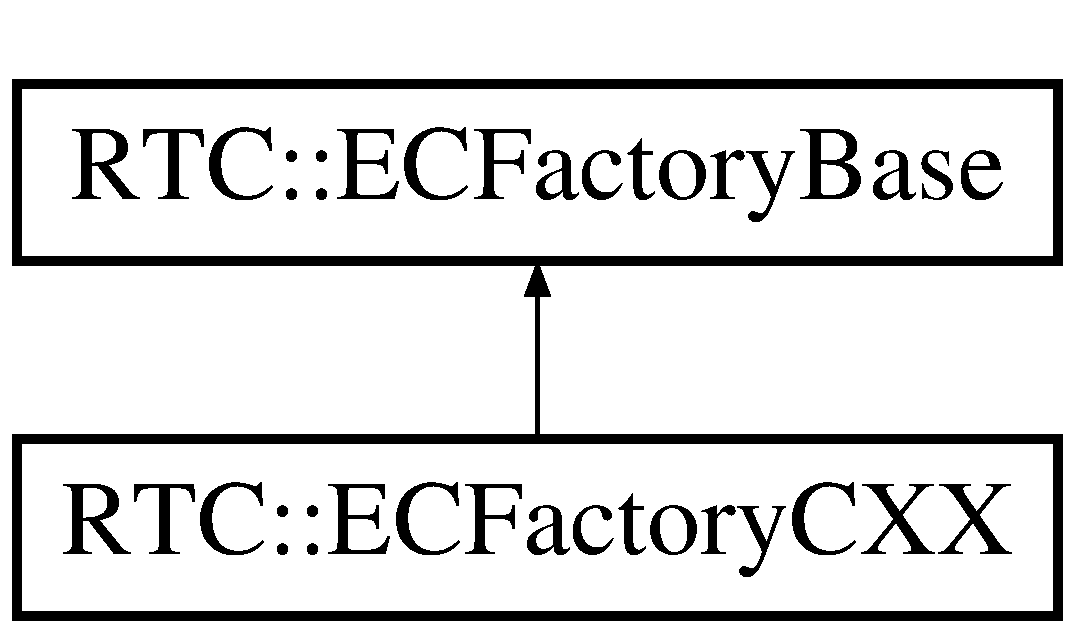
\includegraphics[height=2cm]{classRTC_1_1ECFactoryBase}
\end{center}
\end{figure}
\subsection*{Public メソッド}
\begin{DoxyCompactItemize}
\item 
virtual {\bf $\sim$ECFactoryBase} (void)
\begin{DoxyCompactList}\small\item\em 仮想デストラクタ \item\end{DoxyCompactList}\item 
virtual const char $\ast$ {\bf name} ()=0
\begin{DoxyCompactList}\small\item\em 生成対象ExecutionContext名称取得用純粋仮想関数 \item\end{DoxyCompactList}\item 
virtual {\bf ExecutionContextBase} $\ast$ {\bf create} ()=0
\begin{DoxyCompactList}\small\item\em ExecutionContext生成用純粋仮想関数. \item\end{DoxyCompactList}\item 
virtual void {\bf destroy} ({\bf ExecutionContextBase} $\ast$comp)=0
\begin{DoxyCompactList}\small\item\em ExecutionContext破棄用純粋仮想関数. \item\end{DoxyCompactList}\end{DoxyCompactItemize}


\subsection{説明}
\doxyref{ECFactoryBase}{p.}{classRTC_1_1ECFactoryBase} 抽象クラス. ExecutionContext生成用Factoryの抽象クラス。 各ExecutionContextを生成するための具象Factoryクラスは、 以下の純粋仮想関数の実装を提供しなければならない。

publicインターフェースとして以下のものを提供する。
\begin{DoxyItemize}
\item \doxyref{name()}{p.}{classRTC_1_1ECFactoryBase_a521d5c350bf08586034dc034c46f5c70} : 生成対象ExecutionContext名称の取得
\item \doxyref{create()}{p.}{classRTC_1_1ECFactoryBase_a3a69009a302cb67881576fc407a6cb57} : ExecutionContextインスタンスの生成
\item \doxyref{destroy()}{p.}{classRTC_1_1ECFactoryBase_ad9eeff1fd2bdece6e696bc23eb6e9bcc}: ExecutionContextインスタンスの破棄
\end{DoxyItemize}

\begin{DoxySince}{から}
0.4.0 
\end{DoxySince}


\subsection{コンストラクタとデストラクタ}
\index{RTC::ECFactoryBase@{RTC::ECFactoryBase}!$\sim$ECFactoryBase@{$\sim$ECFactoryBase}}
\index{$\sim$ECFactoryBase@{$\sim$ECFactoryBase}!RTC::ECFactoryBase@{RTC::ECFactoryBase}}
\subsubsection[{$\sim$ECFactoryBase}]{\setlength{\rightskip}{0pt plus 5cm}virtual RTC::ECFactoryBase::$\sim$ECFactoryBase (void)\hspace{0.3cm}{\ttfamily  [inline, virtual]}}\label{classRTC_1_1ECFactoryBase_ab80a647333b628435c91c63982f5498c}


仮想デストラクタ 

仮想デストラクタ。 

\subsection{関数}
\index{RTC::ECFactoryBase@{RTC::ECFactoryBase}!create@{create}}
\index{create@{create}!RTC::ECFactoryBase@{RTC::ECFactoryBase}}
\subsubsection[{create}]{\setlength{\rightskip}{0pt plus 5cm}virtual {\bf ExecutionContextBase}$\ast$ RTC::ECFactoryBase::create ()\hspace{0.3cm}{\ttfamily  [pure virtual]}}\label{classRTC_1_1ECFactoryBase_a3a69009a302cb67881576fc407a6cb57}


ExecutionContext生成用純粋仮想関数. 

ExecutionContextのインスタンスを生成するための純粋仮想関数。

\begin{DoxyReturn}{戻り値}
生成したExecutionContextインスタンス 
\end{DoxyReturn}


{\bf RTC::ECFactoryCXX} \doxyref{}{p.}{classRTC_1_1ECFactoryCXX_a3b9c612725a509f21908105334f2bc36}で実装されています。

\index{RTC::ECFactoryBase@{RTC::ECFactoryBase}!destroy@{destroy}}
\index{destroy@{destroy}!RTC::ECFactoryBase@{RTC::ECFactoryBase}}
\subsubsection[{destroy}]{\setlength{\rightskip}{0pt plus 5cm}virtual void RTC::ECFactoryBase::destroy ({\bf ExecutionContextBase} $\ast$ {\em comp})\hspace{0.3cm}{\ttfamily  [pure virtual]}}\label{classRTC_1_1ECFactoryBase_ad9eeff1fd2bdece6e696bc23eb6e9bcc}


ExecutionContext破棄用純粋仮想関数. 

ExecutionContextのインスタンスを破棄するための純粋仮想関数。


\begin{DoxyParams}{引数}
\item[{\em comp}]破棄対象のExecutionContextインスタンス \end{DoxyParams}


{\bf RTC::ECFactoryCXX} \doxyref{}{p.}{classRTC_1_1ECFactoryCXX_a57dbab7164220dd469c3d23cf36ff721}で実装されています。

\index{RTC::ECFactoryBase@{RTC::ECFactoryBase}!name@{name}}
\index{name@{name}!RTC::ECFactoryBase@{RTC::ECFactoryBase}}
\subsubsection[{name}]{\setlength{\rightskip}{0pt plus 5cm}virtual const char$\ast$ RTC::ECFactoryBase::name ()\hspace{0.3cm}{\ttfamily  [pure virtual]}}\label{classRTC_1_1ECFactoryBase_a521d5c350bf08586034dc034c46f5c70}


生成対象ExecutionContext名称取得用純粋仮想関数 

生成対象ExecutionContextの名称を取得するための純粋仮想関数。

\begin{DoxyReturn}{戻り値}
生成対象ExecutionContext名称 
\end{DoxyReturn}


{\bf RTC::ECFactoryCXX} \doxyref{}{p.}{classRTC_1_1ECFactoryCXX_a7de52069a2c215b6fb4757b4cbe378ec}で実装されています。



参照元 RTC::Manager::ECFactoryPredicate::operator()().


\section{RTC::ECFactoryCXX Class Reference}
\label{classRTC_1_1ECFactoryCXX}\index{RTC::ECFactoryCXX@{RTC::ECFactoryCXX}}


\doxyref{ECFactoryCXX}{p.}{classRTC_1_1ECFactoryCXX} class.  




{\ttfamily \#include $<$ECFactory.h$>$}

Inheritance diagram for RTC::ECFactoryCXX:\begin{figure}[H]
\begin{center}
\leavevmode
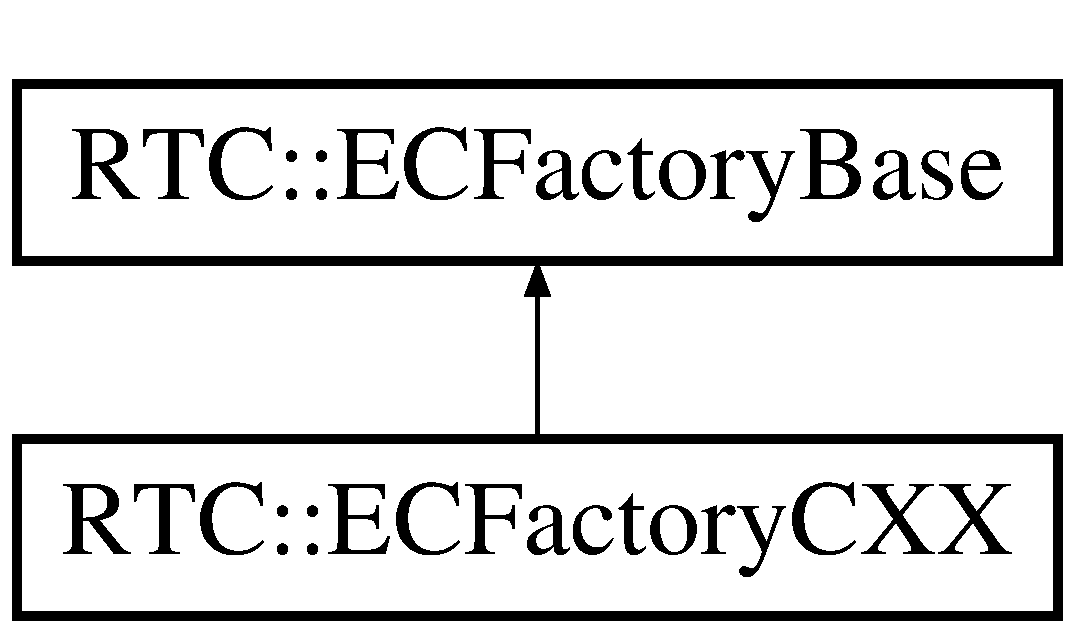
\includegraphics[height=2cm]{classRTC_1_1ECFactoryCXX}
\end{center}
\end{figure}
\subsection*{Public Member Functions}
\begin{DoxyCompactItemize}
\item 
{\bf ECFactoryCXX} (const char $\ast$name, {\bf ECNewFunc} new\_\-func, {\bf ECDeleteFunc} delete\_\-func)
\begin{DoxyCompactList}\small\item\em Constructor. \item\end{DoxyCompactList}\item 
{\bf $\sim$ECFactoryCXX} (void)
\item 
virtual const char $\ast$ {\bf name} ()
\begin{DoxyCompactList}\small\item\em Get names of the target ExecutionContext for creation. \item\end{DoxyCompactList}\item 
virtual {\bf ExecutionContextBase} $\ast$ {\bf create} ()
\begin{DoxyCompactList}\small\item\em Create the target ExecutionContext's instances. \item\end{DoxyCompactList}\item 
virtual void {\bf destroy} ({\bf ExecutionContextBase} $\ast$comp)
\begin{DoxyCompactList}\small\item\em Destroy the target ExecutionContext's instances. \item\end{DoxyCompactList}\end{DoxyCompactItemize}
\subsection*{Protected Attributes}
\begin{DoxyCompactItemize}
\item 
std::string {\bf m\_\-name}
\begin{DoxyCompactList}\small\item\em Names of the target ExecutionContext for creation. \item\end{DoxyCompactList}\item 
{\bf ECNewFunc} {\bf m\_\-New}
\begin{DoxyCompactList}\small\item\em Function to create the target ExecutionContext. \item\end{DoxyCompactList}\item 
{\bf ECDeleteFunc} {\bf m\_\-Delete}
\begin{DoxyCompactList}\small\item\em Function to destroy the target ExecutionContext. \item\end{DoxyCompactList}\end{DoxyCompactItemize}


\subsection{Detailed Description}
\doxyref{ECFactoryCXX}{p.}{classRTC_1_1ECFactoryCXX} class. Factory class to create the ExecutionContext's instances for C++.

\begin{DoxySince}{Since}
0.4.0 
\end{DoxySince}


\subsection{Constructor \& Destructor Documentation}
\index{RTC::ECFactoryCXX@{RTC::ECFactoryCXX}!ECFactoryCXX@{ECFactoryCXX}}
\index{ECFactoryCXX@{ECFactoryCXX}!RTC::ECFactoryCXX@{RTC::ECFactoryCXX}}
\subsubsection[{ECFactoryCXX}]{\setlength{\rightskip}{0pt plus 5cm}RTC::ECFactoryCXX::ECFactoryCXX (const char $\ast$ {\em name}, \/  {\bf ECNewFunc} {\em new\_\-func}, \/  {\bf ECDeleteFunc} {\em delete\_\-func})}\label{classRTC_1_1ECFactoryCXX_a2e7a2762ae32cea607e448b64b71db4f}


Constructor. 

Constructor


\begin{DoxyParams}{Parameters}
\item[{\em name}]Name of the target ExecutionContext for creation \item[{\em new\_\-func}]Function to create ExecutionContext \item[{\em delete\_\-func}]Function to destroy ExecutionContext \end{DoxyParams}
\index{RTC::ECFactoryCXX@{RTC::ECFactoryCXX}!$\sim$ECFactoryCXX@{$\sim$ECFactoryCXX}}
\index{$\sim$ECFactoryCXX@{$\sim$ECFactoryCXX}!RTC::ECFactoryCXX@{RTC::ECFactoryCXX}}
\subsubsection[{$\sim$ECFactoryCXX}]{\setlength{\rightskip}{0pt plus 5cm}RTC::ECFactoryCXX::$\sim$ECFactoryCXX (void)}\label{classRTC_1_1ECFactoryCXX_a590418963cdbd6bcf38e75b61b9ddaee}
Virtual destructor. 

\subsection{Member Function Documentation}
\index{RTC::ECFactoryCXX@{RTC::ECFactoryCXX}!create@{create}}
\index{create@{create}!RTC::ECFactoryCXX@{RTC::ECFactoryCXX}}
\subsubsection[{create}]{\setlength{\rightskip}{0pt plus 5cm}virtual {\bf ExecutionContextBase}$\ast$ RTC::ECFactoryCXX::create ()\hspace{0.3cm}{\ttfamily  [virtual]}}\label{classRTC_1_1ECFactoryCXX_a3b9c612725a509f21908105334f2bc36}


Create the target ExecutionContext's instances. 

Create the target ExecutionContext class's instances.

\begin{DoxyReturn}{Returns}
Created ExecutionContext's instances 
\end{DoxyReturn}


Implements {\bf RTC::ECFactoryBase} \doxyref{}{p.}{classRTC_1_1ECFactoryBase_a3a69009a302cb67881576fc407a6cb57}.

\index{RTC::ECFactoryCXX@{RTC::ECFactoryCXX}!destroy@{destroy}}
\index{destroy@{destroy}!RTC::ECFactoryCXX@{RTC::ECFactoryCXX}}
\subsubsection[{destroy}]{\setlength{\rightskip}{0pt plus 5cm}virtual void RTC::ECFactoryCXX::destroy ({\bf ExecutionContextBase} $\ast$ {\em comp})\hspace{0.3cm}{\ttfamily  [virtual]}}\label{classRTC_1_1ECFactoryCXX_a57dbab7164220dd469c3d23cf36ff721}


Destroy the target ExecutionContext's instances. 

Destroy the target ExecutionContext's instances.


\begin{DoxyParams}{Parameters}
\item[{\em comp}]The target ExecutionContext's instances to destroy \end{DoxyParams}


Implements {\bf RTC::ECFactoryBase} \doxyref{}{p.}{classRTC_1_1ECFactoryBase_ad9eeff1fd2bdece6e696bc23eb6e9bcc}.

\index{RTC::ECFactoryCXX@{RTC::ECFactoryCXX}!name@{name}}
\index{name@{name}!RTC::ECFactoryCXX@{RTC::ECFactoryCXX}}
\subsubsection[{name}]{\setlength{\rightskip}{0pt plus 5cm}virtual const char$\ast$ RTC::ECFactoryCXX::name ()\hspace{0.3cm}{\ttfamily  [virtual]}}\label{classRTC_1_1ECFactoryCXX_a7de52069a2c215b6fb4757b4cbe378ec}


Get names of the target ExecutionContext for creation. 

Get names of the target ExecutionContext for creation.

\begin{DoxyReturn}{Returns}
Names of target ExecutionContext for creation 
\end{DoxyReturn}


Implements {\bf RTC::ECFactoryBase} \doxyref{}{p.}{classRTC_1_1ECFactoryBase_a521d5c350bf08586034dc034c46f5c70}.



\subsection{Member Data Documentation}
\index{RTC::ECFactoryCXX@{RTC::ECFactoryCXX}!m\_\-Delete@{m\_\-Delete}}
\index{m\_\-Delete@{m\_\-Delete}!RTC::ECFactoryCXX@{RTC::ECFactoryCXX}}
\subsubsection[{m\_\-Delete}]{\setlength{\rightskip}{0pt plus 5cm}{\bf ECDeleteFunc} {\bf RTC::ECFactoryCXX::m\_\-Delete}\hspace{0.3cm}{\ttfamily  [protected]}}\label{classRTC_1_1ECFactoryCXX_a74a87e7532e5693799961389f6c397c8}


Function to destroy the target ExecutionContext. 

\index{RTC::ECFactoryCXX@{RTC::ECFactoryCXX}!m\_\-name@{m\_\-name}}
\index{m\_\-name@{m\_\-name}!RTC::ECFactoryCXX@{RTC::ECFactoryCXX}}
\subsubsection[{m\_\-name}]{\setlength{\rightskip}{0pt plus 5cm}std::string {\bf RTC::ECFactoryCXX::m\_\-name}\hspace{0.3cm}{\ttfamily  [protected]}}\label{classRTC_1_1ECFactoryCXX_adf4b96999d4f3bec518ffb3dfd27a57e}


Names of the target ExecutionContext for creation. 

\index{RTC::ECFactoryCXX@{RTC::ECFactoryCXX}!m\_\-New@{m\_\-New}}
\index{m\_\-New@{m\_\-New}!RTC::ECFactoryCXX@{RTC::ECFactoryCXX}}
\subsubsection[{m\_\-New}]{\setlength{\rightskip}{0pt plus 5cm}{\bf ECNewFunc} {\bf RTC::ECFactoryCXX::m\_\-New}\hspace{0.3cm}{\ttfamily  [protected]}}\label{classRTC_1_1ECFactoryCXX_a0665c1d3150e57bb2373fa9bac7e1b06}


Function to create the target ExecutionContext. 


\section{構造体 RTC::Manager::ECFactoryPredicate}
\label{structRTC_1_1Manager_1_1ECFactoryPredicate}\index{RTC::Manager::ECFactoryPredicate@{RTC::Manager::ECFactoryPredicate}}


{\ttfamily \#include $<$Manager.h$>$}

\subsection*{Public メソッド}
\begin{DoxyCompactItemize}
\item 
{\bf ECFactoryPredicate} (const char $\ast$name)
\item 
{\bf ECFactoryPredicate} ({\bf ECFactoryBase} $\ast$factory)
\item 
bool {\bf operator()} ({\bf ECFactoryBase} $\ast$factory)
\end{DoxyCompactItemize}
\subsection*{Public 変数}
\begin{DoxyCompactItemize}
\item 
std::string {\bf m\_\-name}
\end{DoxyCompactItemize}


\subsection{コンストラクタとデストラクタ}
\index{RTC::Manager::ECFactoryPredicate@{RTC::Manager::ECFactoryPredicate}!ECFactoryPredicate@{ECFactoryPredicate}}
\index{ECFactoryPredicate@{ECFactoryPredicate}!RTC::Manager::ECFactoryPredicate@{RTC::Manager::ECFactoryPredicate}}
\subsubsection[{ECFactoryPredicate}]{\setlength{\rightskip}{0pt plus 5cm}RTC::Manager::ECFactoryPredicate::ECFactoryPredicate (const char $\ast$ {\em name})\hspace{0.3cm}{\ttfamily  [inline]}}\label{structRTC_1_1Manager_1_1ECFactoryPredicate_acb95e8e1a216995c855c71cf7434e1b5}
\index{RTC::Manager::ECFactoryPredicate@{RTC::Manager::ECFactoryPredicate}!ECFactoryPredicate@{ECFactoryPredicate}}
\index{ECFactoryPredicate@{ECFactoryPredicate}!RTC::Manager::ECFactoryPredicate@{RTC::Manager::ECFactoryPredicate}}
\subsubsection[{ECFactoryPredicate}]{\setlength{\rightskip}{0pt plus 5cm}RTC::Manager::ECFactoryPredicate::ECFactoryPredicate ({\bf ECFactoryBase} $\ast$ {\em factory})\hspace{0.3cm}{\ttfamily  [inline]}}\label{structRTC_1_1Manager_1_1ECFactoryPredicate_a11d231c5d1145dee8137703c7dd1ad5c}


\subsection{関数}
\index{RTC::Manager::ECFactoryPredicate@{RTC::Manager::ECFactoryPredicate}!operator()@{operator()}}
\index{operator()@{operator()}!RTC::Manager::ECFactoryPredicate@{RTC::Manager::ECFactoryPredicate}}
\subsubsection[{operator()}]{\setlength{\rightskip}{0pt plus 5cm}bool RTC::Manager::ECFactoryPredicate::operator() ({\bf ECFactoryBase} $\ast$ {\em factory})\hspace{0.3cm}{\ttfamily  [inline]}}\label{structRTC_1_1Manager_1_1ECFactoryPredicate_a35e4b2a94d5093eb1c4475d8385d7dbd}


参照先 m\_\-name, と RTC::ECFactoryBase::name().



\subsection{変数}
\index{RTC::Manager::ECFactoryPredicate@{RTC::Manager::ECFactoryPredicate}!m\_\-name@{m\_\-name}}
\index{m\_\-name@{m\_\-name}!RTC::Manager::ECFactoryPredicate@{RTC::Manager::ECFactoryPredicate}}
\subsubsection[{m\_\-name}]{\setlength{\rightskip}{0pt plus 5cm}std::string {\bf RTC::Manager::ECFactoryPredicate::m\_\-name}}\label{structRTC_1_1Manager_1_1ECFactoryPredicate_a3909d7800075eec8117fef8cc864a067}


参照元 operator()().


\section{RTC::ModuleManager::Error Struct Reference}
\label{structRTC_1_1ModuleManager_1_1Error}\index{RTC::ModuleManager::Error@{RTC::ModuleManager::Error}}


Structure for exception handling when file open is failed.  




{\ttfamily \#include $<$ModuleManager.h$>$}

Inheritance diagram for RTC::ModuleManager::Error:\begin{figure}[H]
\begin{center}
\leavevmode
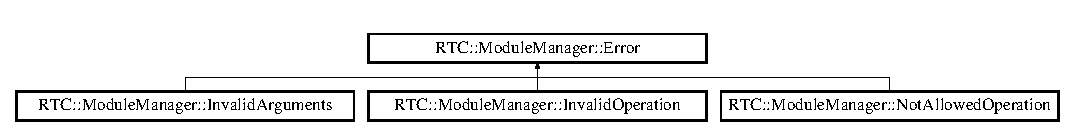
\includegraphics[height=1.38786cm]{structRTC_1_1ModuleManager_1_1Error}
\end{center}
\end{figure}
\subsection*{Public Member Functions}
\begin{DoxyCompactItemize}
\item 
{\bf Error} (const std::string \&\_\-reason)
\end{DoxyCompactItemize}
\subsection*{Public Attributes}
\begin{DoxyCompactItemize}
\item 
std::string {\bf reason}
\end{DoxyCompactItemize}


\subsection{Detailed Description}
Structure for exception handling when file open is failed. 

\subsection{Constructor \& Destructor Documentation}
\index{RTC::ModuleManager::Error@{RTC::ModuleManager::Error}!Error@{Error}}
\index{Error@{Error}!RTC::ModuleManager::Error@{RTC::ModuleManager::Error}}
\subsubsection[{Error}]{\setlength{\rightskip}{0pt plus 5cm}RTC::ModuleManager::Error::Error (const std::string \& {\em \_\-reason})\hspace{0.3cm}{\ttfamily  [inline]}}\label{structRTC_1_1ModuleManager_1_1Error_a56f039f9b9dbb5917cce4e9cd99ce01b}


\subsection{Member Data Documentation}
\index{RTC::ModuleManager::Error@{RTC::ModuleManager::Error}!reason@{reason}}
\index{reason@{reason}!RTC::ModuleManager::Error@{RTC::ModuleManager::Error}}
\subsubsection[{reason}]{\setlength{\rightskip}{0pt plus 5cm}std::string {\bf RTC::ModuleManager::Error::reason}}\label{structRTC_1_1ModuleManager_1_1Error_a0061f5a32edb04ca1376b20675f96b3f}

\section{RTC::ExecutionContextActionListener Class Reference}
\label{classRTC_1_1ExecutionContextActionListener}\index{RTC::ExecutionContextActionListener@{RTC::ExecutionContextActionListener}}


\doxyref{ExecutionContextActionListener}{p.}{classRTC_1_1ExecutionContextActionListener} class.  




{\ttfamily \#include $<$ComponentActionListener.h$>$}

\subsection*{Public Member Functions}
\begin{DoxyCompactItemize}
\item 
virtual {\bf $\sim$ExecutionContextActionListener} ()
\begin{DoxyCompactList}\small\item\em Destructor. \item\end{DoxyCompactList}\item 
virtual void {\bf operator()} ({\bf UniqueId} ec\_\-id)=0
\begin{DoxyCompactList}\small\item\em Virtual Callback function. \item\end{DoxyCompactList}\end{DoxyCompactItemize}
\subsection*{Static Public Member Functions}
\begin{DoxyCompactItemize}
\item 
static const char $\ast$ {\bf toString} ({\bf ExecutionContextActionListenerType} type)
\begin{DoxyCompactList}\small\item\em Convert PreComponentActionListenerType into the string. \item\end{DoxyCompactList}\end{DoxyCompactItemize}


\subsection{Detailed Description}
\doxyref{ExecutionContextActionListener}{p.}{classRTC_1_1ExecutionContextActionListener} class. This class is abstract base class for listener classes that provides callbacks for various events in rtobject. 

\subsection{Constructor \& Destructor Documentation}
\index{RTC::ExecutionContextActionListener@{RTC::ExecutionContextActionListener}!$\sim$ExecutionContextActionListener@{$\sim$ExecutionContextActionListener}}
\index{$\sim$ExecutionContextActionListener@{$\sim$ExecutionContextActionListener}!RTC::ExecutionContextActionListener@{RTC::ExecutionContextActionListener}}
\subsubsection[{$\sim$ExecutionContextActionListener}]{\setlength{\rightskip}{0pt plus 5cm}virtual RTC::ExecutionContextActionListener::$\sim$ExecutionContextActionListener ()\hspace{0.3cm}{\ttfamily  [virtual]}}\label{classRTC_1_1ExecutionContextActionListener_a1fb1f35df22c9154123dcb3a95f2b61a}


Destructor. 



\subsection{Member Function Documentation}
\index{RTC::ExecutionContextActionListener@{RTC::ExecutionContextActionListener}!operator()@{operator()}}
\index{operator()@{operator()}!RTC::ExecutionContextActionListener@{RTC::ExecutionContextActionListener}}
\subsubsection[{operator()}]{\setlength{\rightskip}{0pt plus 5cm}virtual void RTC::ExecutionContextActionListener::operator() ({\bf UniqueId} {\em ec\_\-id})\hspace{0.3cm}{\ttfamily  [pure virtual]}}\label{classRTC_1_1ExecutionContextActionListener_ad899dc2caf7982525bca5ad5c399b989}


Virtual Callback function. 

This is a the Callback function for \doxyref{ExecutionContextActionListener}{p.}{classRTC_1_1ExecutionContextActionListener} \index{RTC::ExecutionContextActionListener@{RTC::ExecutionContextActionListener}!toString@{toString}}
\index{toString@{toString}!RTC::ExecutionContextActionListener@{RTC::ExecutionContextActionListener}}
\subsubsection[{toString}]{\setlength{\rightskip}{0pt plus 5cm}static const char$\ast$ RTC::ExecutionContextActionListener::toString ({\bf ExecutionContextActionListenerType} {\em type})\hspace{0.3cm}{\ttfamily  [inline, static]}}\label{classRTC_1_1ExecutionContextActionListener_a09d31917b4cbdcc69eec0243cafe3d61}


Convert PreComponentActionListenerType into the string. 

Convert PreComponentActionListenerType into the string.


\begin{DoxyParams}{Parameters}
\item[{\em type}]The target PreComponentActionListenerType for transformation\end{DoxyParams}
\begin{DoxyReturn}{Returns}
Trnasformation result of string representation 
\end{DoxyReturn}


References RTC::EC\_\-ACTION\_\-LISTENER\_\-NUM.


\section{クラス RTC::ExecutionContextActionListenerHolder}
\label{classRTC_1_1ExecutionContextActionListenerHolder}\index{RTC::ExecutionContextActionListenerHolder@{RTC::ExecutionContextActionListenerHolder}}


\doxyref{ExecutionContextActionListener}{p.}{classRTC_1_1ExecutionContextActionListener} ホルダクラス.  




{\ttfamily \#include $<$ComponentActionListener.h$>$}

\subsection*{Public メソッド}
\begin{DoxyCompactItemize}
\item 
{\bf ExecutionContextActionListenerHolder} ()
\begin{DoxyCompactList}\small\item\em コンストラクタ \item\end{DoxyCompactList}\item 
virtual {\bf $\sim$ExecutionContextActionListenerHolder} ()
\begin{DoxyCompactList}\small\item\em デストラクタ \item\end{DoxyCompactList}\item 
void {\bf addListener} ({\bf ExecutionContextActionListener} $\ast$listener, bool autoclean)
\begin{DoxyCompactList}\small\item\em リスナーの追加 \item\end{DoxyCompactList}\item 
void {\bf removeListener} ({\bf ExecutionContextActionListener} $\ast$listener)
\begin{DoxyCompactList}\small\item\em リスナーの削除 \item\end{DoxyCompactList}\item 
void {\bf notify} ({\bf UniqueId} ec\_\-id)
\begin{DoxyCompactList}\small\item\em リスナーへ通知する \item\end{DoxyCompactList}\end{DoxyCompactItemize}


\subsection{説明}
\doxyref{ExecutionContextActionListener}{p.}{classRTC_1_1ExecutionContextActionListener} ホルダクラス. 複数の \doxyref{ExecutionContextActionListener}{p.}{classRTC_1_1ExecutionContextActionListener} を保持し管理するクラス。 

\subsection{コンストラクタとデストラクタ}
\index{RTC::ExecutionContextActionListenerHolder@{RTC::ExecutionContextActionListenerHolder}!ExecutionContextActionListenerHolder@{ExecutionContextActionListenerHolder}}
\index{ExecutionContextActionListenerHolder@{ExecutionContextActionListenerHolder}!RTC::ExecutionContextActionListenerHolder@{RTC::ExecutionContextActionListenerHolder}}
\subsubsection[{ExecutionContextActionListenerHolder}]{\setlength{\rightskip}{0pt plus 5cm}RTC::ExecutionContextActionListenerHolder::ExecutionContextActionListenerHolder ()}\label{classRTC_1_1ExecutionContextActionListenerHolder_a422303d2192c9ee6643c202b793311fa}


コンストラクタ 

\index{RTC::ExecutionContextActionListenerHolder@{RTC::ExecutionContextActionListenerHolder}!$\sim$ExecutionContextActionListenerHolder@{$\sim$ExecutionContextActionListenerHolder}}
\index{$\sim$ExecutionContextActionListenerHolder@{$\sim$ExecutionContextActionListenerHolder}!RTC::ExecutionContextActionListenerHolder@{RTC::ExecutionContextActionListenerHolder}}
\subsubsection[{$\sim$ExecutionContextActionListenerHolder}]{\setlength{\rightskip}{0pt plus 5cm}virtual RTC::ExecutionContextActionListenerHolder::$\sim$ExecutionContextActionListenerHolder ()\hspace{0.3cm}{\ttfamily  [virtual]}}\label{classRTC_1_1ExecutionContextActionListenerHolder_ade639d3634de5b385c318decc43f4a57}


デストラクタ 



\subsection{関数}
\index{RTC::ExecutionContextActionListenerHolder@{RTC::ExecutionContextActionListenerHolder}!addListener@{addListener}}
\index{addListener@{addListener}!RTC::ExecutionContextActionListenerHolder@{RTC::ExecutionContextActionListenerHolder}}
\subsubsection[{addListener}]{\setlength{\rightskip}{0pt plus 5cm}void RTC::ExecutionContextActionListenerHolder::addListener ({\bf ExecutionContextActionListener} $\ast$ {\em listener}, \/  bool {\em autoclean})}\label{classRTC_1_1ExecutionContextActionListenerHolder_ad6455f4d2a22c5bdd185294929177286}


リスナーの追加 

リスナーを追加する。


\begin{DoxyParams}{引数}
\item[{\em listener}]追加するリスナ \item[{\em autoclean}]true:デストラクタで削除する, false:デストラクタで削除しない \end{DoxyParams}
\index{RTC::ExecutionContextActionListenerHolder@{RTC::ExecutionContextActionListenerHolder}!notify@{notify}}
\index{notify@{notify}!RTC::ExecutionContextActionListenerHolder@{RTC::ExecutionContextActionListenerHolder}}
\subsubsection[{notify}]{\setlength{\rightskip}{0pt plus 5cm}void RTC::ExecutionContextActionListenerHolder::notify ({\bf UniqueId} {\em ec\_\-id})}\label{classRTC_1_1ExecutionContextActionListenerHolder_afe7d95ed2fb7934e57f6e3b38f041188}


リスナーへ通知する 

登録されているリスナのコールバックメソッドを呼び出す。


\begin{DoxyParams}{引数}
\item[{\em info}]\doxyref{ConnectorInfo}{p.}{classRTC_1_1ConnectorInfo} \item[{\em cdrdata}]データ \end{DoxyParams}


参照元 RTC::RTObject\_\-impl::onAttachExecutionContext(), と RTC::RTObject\_\-impl::onDetachExecutionContext().

\index{RTC::ExecutionContextActionListenerHolder@{RTC::ExecutionContextActionListenerHolder}!removeListener@{removeListener}}
\index{removeListener@{removeListener}!RTC::ExecutionContextActionListenerHolder@{RTC::ExecutionContextActionListenerHolder}}
\subsubsection[{removeListener}]{\setlength{\rightskip}{0pt plus 5cm}void RTC::ExecutionContextActionListenerHolder::removeListener ({\bf ExecutionContextActionListener} $\ast$ {\em listener})}\label{classRTC_1_1ExecutionContextActionListenerHolder_acc2999c9555847e2cec937ac9b89ec56}


リスナーの削除 

リスナを削除する。


\begin{DoxyParams}{引数}
\item[{\em listener}]削除するリスナ \end{DoxyParams}

\section{RTC::ExecutionContextBase Class Reference}
\label{classRTC_1_1ExecutionContextBase}\index{RTC::ExecutionContextBase@{RTC::ExecutionContextBase}}


A base class for ExecutionContext.  




{\ttfamily \#include $<$ExecutionContextBase.h$>$}

Inheritance diagram for RTC::ExecutionContextBase:\begin{figure}[H]
\begin{center}
\leavevmode
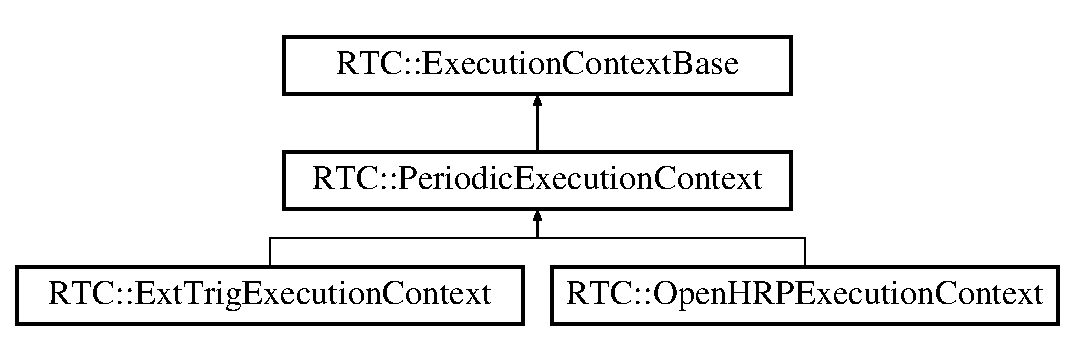
\includegraphics[height=3cm]{classRTC_1_1ExecutionContextBase}
\end{center}
\end{figure}
\subsection*{Public Member Functions}
\begin{DoxyCompactItemize}
\item 
virtual {\bf $\sim$ExecutionContextBase} (void)
\begin{DoxyCompactList}\small\item\em Virtual Destructor. \item\end{DoxyCompactList}\item 
virtual void {\bf tick} ()  throw (CORBA::SystemException)
\begin{DoxyCompactList}\small\item\em Proceed with tick of ExecutionContext. \item\end{DoxyCompactList}\item 
virtual RTC::ReturnCode\_\-t {\bf bindComponent} ({\bf RTObject\_\-impl} $\ast$rtc)=0
\item 
virtual RTC::ExecutionContextService\_\-ptr {\bf getObjRef} ()=0
\end{DoxyCompactItemize}


\subsection{Detailed Description}
A base class for ExecutionContext. A base class of ExecutionContext.

\begin{DoxySince}{Since}
0.4.0 
\end{DoxySince}


\subsection{Constructor \& Destructor Documentation}
\index{RTC::ExecutionContextBase@{RTC::ExecutionContextBase}!$\sim$ExecutionContextBase@{$\sim$ExecutionContextBase}}
\index{$\sim$ExecutionContextBase@{$\sim$ExecutionContextBase}!RTC::ExecutionContextBase@{RTC::ExecutionContextBase}}
\subsubsection[{$\sim$ExecutionContextBase}]{\setlength{\rightskip}{0pt plus 5cm}virtual RTC::ExecutionContextBase::$\sim$ExecutionContextBase (void)\hspace{0.3cm}{\ttfamily  [inline, virtual]}}\label{classRTC_1_1ExecutionContextBase_a3859cce1770696b6e8486e1199b47541}


Virtual Destructor. 

Virtual Destructor 

\subsection{Member Function Documentation}
\index{RTC::ExecutionContextBase@{RTC::ExecutionContextBase}!bindComponent@{bindComponent}}
\index{bindComponent@{bindComponent}!RTC::ExecutionContextBase@{RTC::ExecutionContextBase}}
\subsubsection[{bindComponent}]{\setlength{\rightskip}{0pt plus 5cm}virtual RTC::ReturnCode\_\-t RTC::ExecutionContextBase::bindComponent ({\bf RTObject\_\-impl} $\ast$ {\em rtc})\hspace{0.3cm}{\ttfamily  [pure virtual]}}\label{classRTC_1_1ExecutionContextBase_a63f6427cfe69b5dbc92fa192e26bcf7e}
Bind the component. 

Implemented in {\bf RTC::PeriodicExecutionContext} \doxyref{}{p.}{classRTC_1_1PeriodicExecutionContext_aac9d423142bf3b8d219740a4f202b033}.

\index{RTC::ExecutionContextBase@{RTC::ExecutionContextBase}!getObjRef@{getObjRef}}
\index{getObjRef@{getObjRef}!RTC::ExecutionContextBase@{RTC::ExecutionContextBase}}
\subsubsection[{getObjRef}]{\setlength{\rightskip}{0pt plus 5cm}virtual RTC::ExecutionContextService\_\-ptr RTC::ExecutionContextBase::getObjRef ()\hspace{0.3cm}{\ttfamily  [pure virtual]}}\label{classRTC_1_1ExecutionContextBase_a05d88ee228cc75ab82e2c25c3eafc7db}
Get the reference of the object. 

Implemented in {\bf RTC::PeriodicExecutionContext} \doxyref{}{p.}{classRTC_1_1PeriodicExecutionContext_a24fac023d4758a6297dab92ee8db6610}.

\index{RTC::ExecutionContextBase@{RTC::ExecutionContextBase}!tick@{tick}}
\index{tick@{tick}!RTC::ExecutionContextBase@{RTC::ExecutionContextBase}}
\subsubsection[{tick}]{\setlength{\rightskip}{0pt plus 5cm}virtual void RTC::ExecutionContextBase::tick (void)  throw (CORBA::SystemException)\hspace{0.3cm}{\ttfamily  [inline, virtual]}}\label{classRTC_1_1ExecutionContextBase_a9a72856fe8c46ab49c54042d30c9e343}


Proceed with tick of ExecutionContext. 

Proceed with tick of ExecutionContext for one period. 

Reimplemented in {\bf RTC::ExtTrigExecutionContext} \doxyref{}{p.}{classRTC_1_1ExtTrigExecutionContext_a620fd10cb8d7c5dc3a35d1bb21e06cde}, and {\bf RTC::OpenHRPExecutionContext} \doxyref{}{p.}{classRTC_1_1OpenHRPExecutionContext_a8d48b4067e8f98c350d09b318cf14f60}.


\section{RTC::ExtTrigExecutionContext Class Reference}
\label{classRTC_1_1ExtTrigExecutionContext}\index{RTC::ExtTrigExecutionContext@{RTC::ExtTrigExecutionContext}}


ExecutionContext class that enables one step execution.  




{\ttfamily \#include $<$ExtTrigExecutionContext.h$>$}

Inheritance diagram for RTC::ExtTrigExecutionContext:\begin{figure}[H]
\begin{center}
\leavevmode
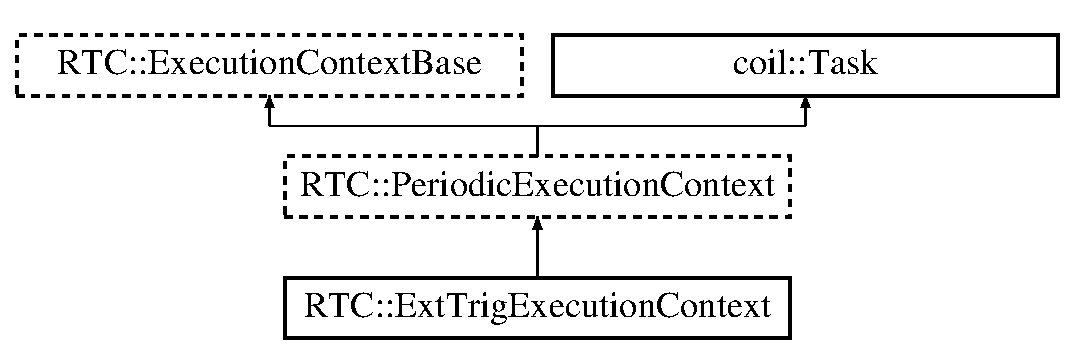
\includegraphics[height=3cm]{classRTC_1_1ExtTrigExecutionContext}
\end{center}
\end{figure}
\subsection*{Classes}
\begin{DoxyCompactItemize}
\item 
struct {\bfseries Worker}
\end{DoxyCompactItemize}
\subsection*{Public Member Functions}
\begin{DoxyCompactItemize}
\item 
{\bf ExtTrigExecutionContext} ()
\begin{DoxyCompactList}\small\item\em Constructor. \item\end{DoxyCompactList}\item 
virtual {\bf $\sim$ExtTrigExecutionContext} (void)
\begin{DoxyCompactList}\small\item\em Destructor. \item\end{DoxyCompactList}\item 
virtual void {\bf tick} ()  throw (CORBA::SystemException)
\begin{DoxyCompactList}\small\item\em Move forward one step of ExecutionContext. \item\end{DoxyCompactList}\item 
virtual int {\bf svc} (void)
\begin{DoxyCompactList}\small\item\em Invoke each component's operation. \item\end{DoxyCompactList}\end{DoxyCompactItemize}


\subsection{Detailed Description}
ExecutionContext class that enables one step execution. ExecutionContext class that can execute every one cycle for Periodic Sampled Data Processing. Time(Tick) advances one cycle by invoking method externally.

\begin{DoxySince}{Since}
0.4.0 
\end{DoxySince}


\subsection{Constructor \& Destructor Documentation}
\index{RTC::ExtTrigExecutionContext@{RTC::ExtTrigExecutionContext}!ExtTrigExecutionContext@{ExtTrigExecutionContext}}
\index{ExtTrigExecutionContext@{ExtTrigExecutionContext}!RTC::ExtTrigExecutionContext@{RTC::ExtTrigExecutionContext}}
\subsubsection[{ExtTrigExecutionContext}]{\setlength{\rightskip}{0pt plus 5cm}RTC::ExtTrigExecutionContext::ExtTrigExecutionContext ()}\label{classRTC_1_1ExtTrigExecutionContext_a203eb6aa27e25fab09a3cb35d471b080}


Constructor. 

Constructor \index{RTC::ExtTrigExecutionContext@{RTC::ExtTrigExecutionContext}!$\sim$ExtTrigExecutionContext@{$\sim$ExtTrigExecutionContext}}
\index{$\sim$ExtTrigExecutionContext@{$\sim$ExtTrigExecutionContext}!RTC::ExtTrigExecutionContext@{RTC::ExtTrigExecutionContext}}
\subsubsection[{$\sim$ExtTrigExecutionContext}]{\setlength{\rightskip}{0pt plus 5cm}virtual RTC::ExtTrigExecutionContext::$\sim$ExtTrigExecutionContext (void)\hspace{0.3cm}{\ttfamily  [virtual]}}\label{classRTC_1_1ExtTrigExecutionContext_a5f931fd6a6fdf84d8c7dedccc5f0b318}


Destructor. 

Destructor 

\subsection{Member Function Documentation}
\index{RTC::ExtTrigExecutionContext@{RTC::ExtTrigExecutionContext}!svc@{svc}}
\index{svc@{svc}!RTC::ExtTrigExecutionContext@{RTC::ExtTrigExecutionContext}}
\subsubsection[{svc}]{\setlength{\rightskip}{0pt plus 5cm}virtual int RTC::ExtTrigExecutionContext::svc (void)\hspace{0.3cm}{\ttfamily  [virtual]}}\label{classRTC_1_1ExtTrigExecutionContext_aaa5d7178bb12669324647eb702629535}


Invoke each component's operation. 

Invoke each component's operation which is attached this ExecutionContext. Stop until the next operation is invoked after all component operations are invoked.

\begin{DoxyReturn}{Returns}
Operation result 
\end{DoxyReturn}


Reimplemented from {\bf RTC::PeriodicExecutionContext} \doxyref{}{p.}{classRTC_1_1PeriodicExecutionContext_acce0ee7c44366398928e688f895af60b}.

\index{RTC::ExtTrigExecutionContext@{RTC::ExtTrigExecutionContext}!tick@{tick}}
\index{tick@{tick}!RTC::ExtTrigExecutionContext@{RTC::ExtTrigExecutionContext}}
\subsubsection[{tick}]{\setlength{\rightskip}{0pt plus 5cm}virtual void RTC::ExtTrigExecutionContext::tick ()  throw (CORBA::SystemException)\hspace{0.3cm}{\ttfamily  [virtual]}}\label{classRTC_1_1ExtTrigExecutionContext_a620fd10cb8d7c5dc3a35d1bb21e06cde}


Move forward one step of ExecutionContext. 

Move forward one step of the ExecutionContext processing. 

Reimplemented from {\bf RTC::ExecutionContextBase} \doxyref{}{p.}{classRTC_1_1ExecutionContextBase_a9a72856fe8c46ab49c54042d30c9e343}.


\section{クラス テンプレート coil::Factory$<$ AbstractClass, Identifier, Compare, Creator, Destructor $>$}
\label{classcoil_1_1Factory}\index{coil::Factory@{coil::Factory}}


\doxyref{Factory}{p.}{classcoil_1_1Factory} テンプレートクラス.  




{\ttfamily \#include $<$Factory.h$>$}

coil::Factory$<$ AbstractClass, Identifier, Compare, Creator, Destructor $>$に対する継承グラフ\begin{figure}[H]
\begin{center}
\leavevmode
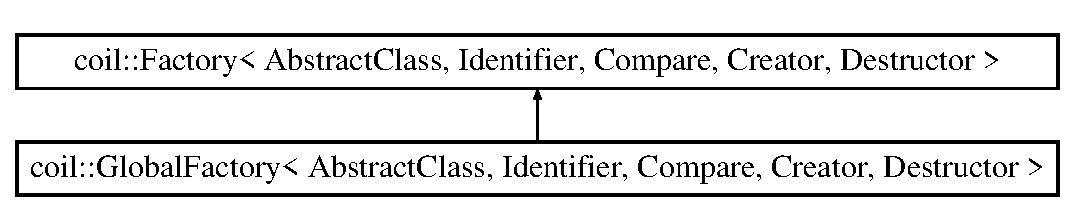
\includegraphics[height=2cm]{classcoil_1_1Factory}
\end{center}
\end{figure}
\subsection*{構成}
\begin{DoxyCompactItemize}
\item 
class {\bfseries FactoryEntry}
\begin{DoxyCompactList}\small\item\em FactoryEntry クラス. \item\end{DoxyCompactList}\end{DoxyCompactItemize}
\subsection*{Public 型}
\begin{DoxyCompactItemize}
\item 
enum {\bf ReturnCode} \{ \par
{\bf FACTORY\_\-OK}, 
{\bf FACTORY\_\-ERROR}, 
{\bf ALREADY\_\-EXISTS}, 
{\bf NOT\_\-FOUND}, 
\par
{\bf INVALID\_\-ARG}, 
{\bf UNKNOWN\_\-ERROR}
 \}
\item 
typedef std::map$<$ Identifier, FactoryEntry $>$ {\bf FactoryMap}
\item 
typedef FactoryMap::iterator {\bf FactoryMapIt}
\end{DoxyCompactItemize}
\subsection*{Public メソッド}
\begin{DoxyCompactItemize}
\item 
bool {\bf hasFactory} (const Identifier \&id)
\begin{DoxyCompactList}\small\item\em ファクトリー有無チェック \item\end{DoxyCompactList}\item 
std::vector$<$ Identifier $>$ {\bf getIdentifiers} ()
\begin{DoxyCompactList}\small\item\em ファクトリーIDリスト取得 \item\end{DoxyCompactList}\item 
{\bf ReturnCode} {\bf addFactory} (const Identifier \&id, Creator creator, Destructor destructor)
\begin{DoxyCompactList}\small\item\em ファクトリー登録 \item\end{DoxyCompactList}\item 
{\bf ReturnCode} {\bf removeFactory} (const Identifier \&id)
\begin{DoxyCompactList}\small\item\em ファクトリー削除 \item\end{DoxyCompactList}\item 
AbstractClass $\ast$ {\bf createObject} (const Identifier \&id)
\begin{DoxyCompactList}\small\item\em ファクトリーオブジェクト生成 \item\end{DoxyCompactList}\item 
void {\bf deleteObject} (const Identifier \&id, AbstractClass $\ast$\&obj)
\begin{DoxyCompactList}\small\item\em ファクトリーオブジェクト削除 \item\end{DoxyCompactList}\item 
void {\bf deleteObject} (AbstractClass $\ast$\&obj)
\begin{DoxyCompactList}\small\item\em ファクトリーオブジェクト削除 \item\end{DoxyCompactList}\end{DoxyCompactItemize}


\subsection{説明}
\subsubsection*{template$<$class AbstractClass, typename Identifier = std::string, typename Compare = std::less$<$Identifier$>$, typename Creator = AbstractClass$\ast$ ($\ast$)(), typename Destructor = void ($\ast$)(AbstractClass$\ast$\&)$>$ class coil::Factory$<$ AbstractClass, Identifier, Compare, Creator, Destructor $>$}

\doxyref{Factory}{p.}{classcoil_1_1Factory} テンプレートクラス. 

\subsection{型定義}
\index{coil::Factory@{coil::Factory}!FactoryMap@{FactoryMap}}
\index{FactoryMap@{FactoryMap}!coil::Factory@{coil::Factory}}
\subsubsection[{FactoryMap}]{\setlength{\rightskip}{0pt plus 5cm}template$<$class AbstractClass , typename Identifier  = std::string, typename Compare  = std::less$<$Identifier$>$, typename Creator  = AbstractClass$\ast$ ($\ast$)(), typename Destructor  = void ($\ast$)(AbstractClass$\ast$\&)$>$ typedef std::map$<$Identifier, FactoryEntry$>$ {\bf coil::Factory}$<$ AbstractClass, Identifier, Compare, Creator, Destructor $>$::{\bf FactoryMap}}\label{classcoil_1_1Factory_ab061a29a06208bd555d18a0cec31643e}
\index{coil::Factory@{coil::Factory}!FactoryMapIt@{FactoryMapIt}}
\index{FactoryMapIt@{FactoryMapIt}!coil::Factory@{coil::Factory}}
\subsubsection[{FactoryMapIt}]{\setlength{\rightskip}{0pt plus 5cm}template$<$class AbstractClass , typename Identifier  = std::string, typename Compare  = std::less$<$Identifier$>$, typename Creator  = AbstractClass$\ast$ ($\ast$)(), typename Destructor  = void ($\ast$)(AbstractClass$\ast$\&)$>$ typedef FactoryMap::iterator {\bf coil::Factory}$<$ AbstractClass, Identifier, Compare, Creator, Destructor $>$::{\bf FactoryMapIt}}\label{classcoil_1_1Factory_a3f166d1a15f75685bc71f26818b3742e}


\subsection{列挙型}
\index{coil::Factory@{coil::Factory}!ReturnCode@{ReturnCode}}
\index{ReturnCode@{ReturnCode}!coil::Factory@{coil::Factory}}
\subsubsection[{ReturnCode}]{\setlength{\rightskip}{0pt plus 5cm}template$<$class AbstractClass , typename Identifier  = std::string, typename Compare  = std::less$<$Identifier$>$, typename Creator  = AbstractClass$\ast$ ($\ast$)(), typename Destructor  = void ($\ast$)(AbstractClass$\ast$\&)$>$ enum {\bf coil::Factory::ReturnCode}}\label{classcoil_1_1Factory_ad3daf45b88091bf7eded408aff26767e}
\begin{Desc}
\item[列挙型の値: ]\par
\begin{description}
\index{FACTORY\_\-OK@{FACTORY\_\-OK}!coil::Factory@{coil::Factory}}\index{coil::Factory@{coil::Factory}!FACTORY\_\-OK@{FACTORY\_\-OK}}\item[{\em 
FACTORY\_\-OK\label{classcoil_1_1Factory_ad3daf45b88091bf7eded408aff26767ea784faadaad92a19ebdf5e46bc51797bc}
}]\index{FACTORY\_\-ERROR@{FACTORY\_\-ERROR}!coil::Factory@{coil::Factory}}\index{coil::Factory@{coil::Factory}!FACTORY\_\-ERROR@{FACTORY\_\-ERROR}}\item[{\em 
FACTORY\_\-ERROR\label{classcoil_1_1Factory_ad3daf45b88091bf7eded408aff26767ea83232a6633f9253871a7e394d0579af1}
}]\index{ALREADY\_\-EXISTS@{ALREADY\_\-EXISTS}!coil::Factory@{coil::Factory}}\index{coil::Factory@{coil::Factory}!ALREADY\_\-EXISTS@{ALREADY\_\-EXISTS}}\item[{\em 
ALREADY\_\-EXISTS\label{classcoil_1_1Factory_ad3daf45b88091bf7eded408aff26767ea775603a29140211fb2a075a8dc8c15a8}
}]\index{NOT\_\-FOUND@{NOT\_\-FOUND}!coil::Factory@{coil::Factory}}\index{coil::Factory@{coil::Factory}!NOT\_\-FOUND@{NOT\_\-FOUND}}\item[{\em 
NOT\_\-FOUND\label{classcoil_1_1Factory_ad3daf45b88091bf7eded408aff26767ead089df73956ca711b29d1231202c534f}
}]\index{INVALID\_\-ARG@{INVALID\_\-ARG}!coil::Factory@{coil::Factory}}\index{coil::Factory@{coil::Factory}!INVALID\_\-ARG@{INVALID\_\-ARG}}\item[{\em 
INVALID\_\-ARG\label{classcoil_1_1Factory_ad3daf45b88091bf7eded408aff26767ea8295bf74c563b880f6a05424192e5721}
}]\index{UNKNOWN\_\-ERROR@{UNKNOWN\_\-ERROR}!coil::Factory@{coil::Factory}}\index{coil::Factory@{coil::Factory}!UNKNOWN\_\-ERROR@{UNKNOWN\_\-ERROR}}\item[{\em 
UNKNOWN\_\-ERROR\label{classcoil_1_1Factory_ad3daf45b88091bf7eded408aff26767ea752306a145550a11ad7a374800b76c1f}
}]\end{description}
\end{Desc}



\subsection{関数}
\index{coil::Factory@{coil::Factory}!addFactory@{addFactory}}
\index{addFactory@{addFactory}!coil::Factory@{coil::Factory}}
\subsubsection[{addFactory}]{\setlength{\rightskip}{0pt plus 5cm}template$<$class AbstractClass , typename Identifier  = std::string, typename Compare  = std::less$<$Identifier$>$, typename Creator  = AbstractClass$\ast$ ($\ast$)(), typename Destructor  = void ($\ast$)(AbstractClass$\ast$\&)$>$ {\bf ReturnCode} {\bf coil::Factory}$<$ AbstractClass, Identifier, Compare, Creator, Destructor $>$::addFactory (const Identifier \& {\em id}, \/  Creator {\em creator}, \/  Destructor {\em destructor})\hspace{0.3cm}{\ttfamily  [inline]}}\label{classcoil_1_1Factory_a16c7d1aa9d9b47a5047831c3d7cb8cea}


ファクトリー登録 

ファクトリーを登録する。


\begin{DoxyParams}{引数}
\item[{\em id}]ファクトリーID \item[{\em creator}]クリエータ用ファンクタ \item[{\em destructor}]デストラクタ用ファンクタ\end{DoxyParams}
\begin{DoxyReturn}{戻り値}
FACTORY\_\-OK: 正常終了 ALREADY\_\-EXISTS: 登録済み INVALID\_\-ARG: creator か destructor が不正な値を含む 
\end{DoxyReturn}
\index{coil::Factory@{coil::Factory}!createObject@{createObject}}
\index{createObject@{createObject}!coil::Factory@{coil::Factory}}
\subsubsection[{createObject}]{\setlength{\rightskip}{0pt plus 5cm}template$<$class AbstractClass , typename Identifier  = std::string, typename Compare  = std::less$<$Identifier$>$, typename Creator  = AbstractClass$\ast$ ($\ast$)(), typename Destructor  = void ($\ast$)(AbstractClass$\ast$\&)$>$ AbstractClass$\ast$ {\bf coil::Factory}$<$ AbstractClass, Identifier, Compare, Creator, Destructor $>$::createObject (const Identifier \& {\em id})\hspace{0.3cm}{\ttfamily  [inline]}}\label{classcoil_1_1Factory_abfe2f51244047f026f1e86bef7880220}


ファクトリーオブジェクト生成 

ファクトリーオブジェクトを生成する。


\begin{DoxyParams}{引数}
\item[{\em id}]ファクトリーID\end{DoxyParams}
\begin{DoxyReturn}{戻り値}
AbstractClass のポインタ 
\end{DoxyReturn}
\index{coil::Factory@{coil::Factory}!deleteObject@{deleteObject}}
\index{deleteObject@{deleteObject}!coil::Factory@{coil::Factory}}
\subsubsection[{deleteObject}]{\setlength{\rightskip}{0pt plus 5cm}template$<$class AbstractClass , typename Identifier  = std::string, typename Compare  = std::less$<$Identifier$>$, typename Creator  = AbstractClass$\ast$ ($\ast$)(), typename Destructor  = void ($\ast$)(AbstractClass$\ast$\&)$>$ void {\bf coil::Factory}$<$ AbstractClass, Identifier, Compare, Creator, Destructor $>$::deleteObject (AbstractClass $\ast$\& {\em obj})\hspace{0.3cm}{\ttfamily  [inline]}}\label{classcoil_1_1Factory_a48aaa74f2c0c36dbe7261f94450bbbc2}


ファクトリーオブジェクト削除 

ファクトリーオブジェクトを削除する。


\begin{DoxyParams}{引数}
\item[{\em obj}]ファクトリーオブジェクト \end{DoxyParams}
\index{coil::Factory@{coil::Factory}!deleteObject@{deleteObject}}
\index{deleteObject@{deleteObject}!coil::Factory@{coil::Factory}}
\subsubsection[{deleteObject}]{\setlength{\rightskip}{0pt plus 5cm}template$<$class AbstractClass , typename Identifier  = std::string, typename Compare  = std::less$<$Identifier$>$, typename Creator  = AbstractClass$\ast$ ($\ast$)(), typename Destructor  = void ($\ast$)(AbstractClass$\ast$\&)$>$ void {\bf coil::Factory}$<$ AbstractClass, Identifier, Compare, Creator, Destructor $>$::deleteObject (const Identifier \& {\em id}, \/  AbstractClass $\ast$\& {\em obj})\hspace{0.3cm}{\ttfamily  [inline]}}\label{classcoil_1_1Factory_a3bc2ace6f1d5ef8d7208fdd501d5a78c}


ファクトリーオブジェクト削除 

ファクトリーオブジェクトを削除する。


\begin{DoxyParams}{引数}
\item[{\em id}]ファクトリーID \item[{\em obj}]ファクトリーオブジェクト \end{DoxyParams}
\index{coil::Factory@{coil::Factory}!getIdentifiers@{getIdentifiers}}
\index{getIdentifiers@{getIdentifiers}!coil::Factory@{coil::Factory}}
\subsubsection[{getIdentifiers}]{\setlength{\rightskip}{0pt plus 5cm}template$<$class AbstractClass , typename Identifier  = std::string, typename Compare  = std::less$<$Identifier$>$, typename Creator  = AbstractClass$\ast$ ($\ast$)(), typename Destructor  = void ($\ast$)(AbstractClass$\ast$\&)$>$ std::vector$<$Identifier$>$ {\bf coil::Factory}$<$ AbstractClass, Identifier, Compare, Creator, Destructor $>$::getIdentifiers ()\hspace{0.3cm}{\ttfamily  [inline]}}\label{classcoil_1_1Factory_aa9f653dfebd545ee6af63b339b2e18b5}


ファクトリーIDリスト取得 

ファクトリーIDリストを返す。

\begin{DoxyReturn}{戻り値}
ID リスト 
\end{DoxyReturn}
\index{coil::Factory@{coil::Factory}!hasFactory@{hasFactory}}
\index{hasFactory@{hasFactory}!coil::Factory@{coil::Factory}}
\subsubsection[{hasFactory}]{\setlength{\rightskip}{0pt plus 5cm}template$<$class AbstractClass , typename Identifier  = std::string, typename Compare  = std::less$<$Identifier$>$, typename Creator  = AbstractClass$\ast$ ($\ast$)(), typename Destructor  = void ($\ast$)(AbstractClass$\ast$\&)$>$ bool {\bf coil::Factory}$<$ AbstractClass, Identifier, Compare, Creator, Destructor $>$::hasFactory (const Identifier \& {\em id})\hspace{0.3cm}{\ttfamily  [inline]}}\label{classcoil_1_1Factory_a613021c4ef085965a978cc89bd3b51e2}


ファクトリー有無チェック 

指定IDのファクトリー有無を返す。


\begin{DoxyParams}{引数}
\item[{\em id}]ファクトリーID\end{DoxyParams}
\begin{DoxyReturn}{戻り値}
true: 有り, false: 無し 
\end{DoxyReturn}
\index{coil::Factory@{coil::Factory}!removeFactory@{removeFactory}}
\index{removeFactory@{removeFactory}!coil::Factory@{coil::Factory}}
\subsubsection[{removeFactory}]{\setlength{\rightskip}{0pt plus 5cm}template$<$class AbstractClass , typename Identifier  = std::string, typename Compare  = std::less$<$Identifier$>$, typename Creator  = AbstractClass$\ast$ ($\ast$)(), typename Destructor  = void ($\ast$)(AbstractClass$\ast$\&)$>$ {\bf ReturnCode} {\bf coil::Factory}$<$ AbstractClass, Identifier, Compare, Creator, Destructor $>$::removeFactory (const Identifier \& {\em id})\hspace{0.3cm}{\ttfamily  [inline]}}\label{classcoil_1_1Factory_a4c501f613299acf93d30179e91674f77}


ファクトリー削除 

ファクトリーを削除する。


\begin{DoxyParams}{引数}
\item[{\em id}]ファクトリーID\end{DoxyParams}
\begin{DoxyReturn}{戻り値}
FACTORY\_\-OK: 正常終了 NOT\_\-FOUND: ID未登録 
\end{DoxyReturn}

\section{RTC::FactoryBase Class Reference}
\label{classRTC_1_1FactoryBase}\index{RTC::FactoryBase@{RTC::FactoryBase}}


\doxyref{FactoryBase}{p.}{classRTC_1_1FactoryBase} base class.  




{\ttfamily \#include $<$Factory.h$>$}

Inheritance diagram for RTC::FactoryBase:\begin{figure}[H]
\begin{center}
\leavevmode
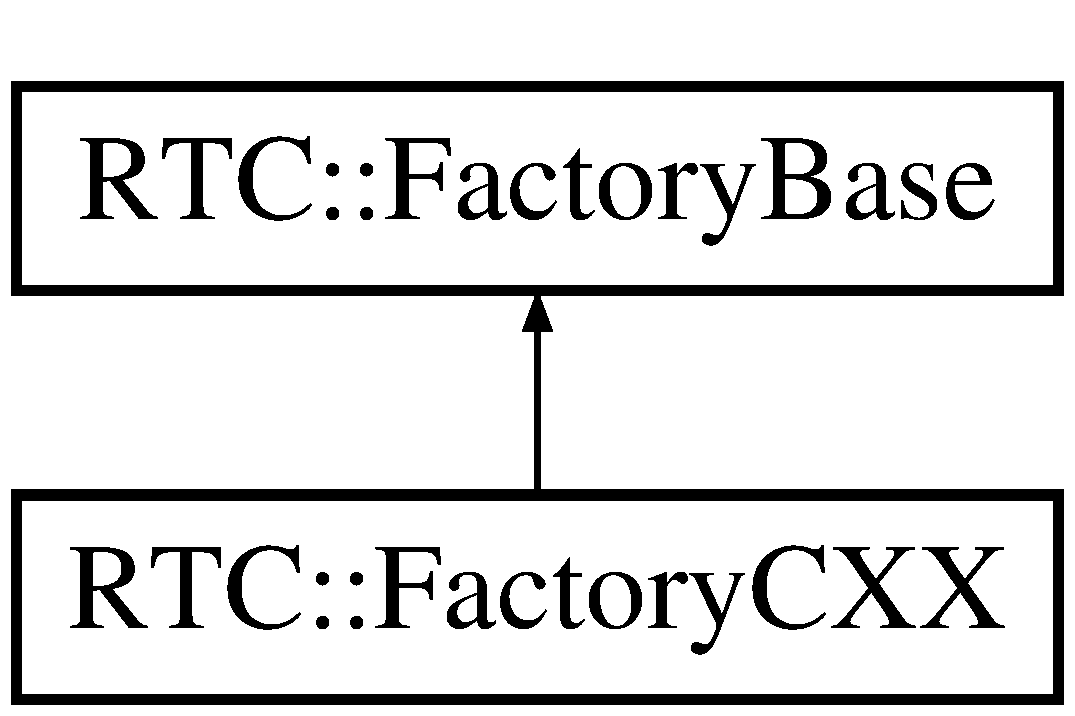
\includegraphics[height=2cm]{classRTC_1_1FactoryBase}
\end{center}
\end{figure}
\subsection*{Public Member Functions}
\begin{DoxyCompactItemize}
\item 
{\bf FactoryBase} (const {\bf coil::Properties} \&profile)
\begin{DoxyCompactList}\small\item\em Constructor. \item\end{DoxyCompactList}\item 
virtual {\bf $\sim$FactoryBase} (void)
\begin{DoxyCompactList}\small\item\em Destructor. \item\end{DoxyCompactList}\item 
virtual {\bf RTObject\_\-impl} $\ast$ {\bf create} ({\bf Manager} $\ast$mgr)=0
\begin{DoxyCompactList}\small\item\em Create components. \item\end{DoxyCompactList}\item 
virtual void {\bf destroy} ({\bf RTObject\_\-impl} $\ast$comp)=0
\begin{DoxyCompactList}\small\item\em Destroy components. \item\end{DoxyCompactList}\item 
virtual {\bf coil::Properties} \& {\bf profile} ()
\begin{DoxyCompactList}\small\item\em Get the component profile. \item\end{DoxyCompactList}\item 
virtual int {\bf number} ()
\begin{DoxyCompactList}\small\item\em Get the number of current instances. \item\end{DoxyCompactList}\end{DoxyCompactItemize}
\subsection*{Protected Attributes}
\begin{DoxyCompactItemize}
\item 
{\bf coil::Properties} {\bf m\_\-Profile}
\begin{DoxyCompactList}\small\item\em Component profile. \item\end{DoxyCompactList}\item 
int {\bf m\_\-Number}
\begin{DoxyCompactList}\small\item\em Number of current RT-\/Component's instances. \item\end{DoxyCompactList}\end{DoxyCompactItemize}


\subsection{Detailed Description}
\doxyref{FactoryBase}{p.}{classRTC_1_1FactoryBase} base class. This is a base class for RT-\/Component factory.

\begin{DoxySince}{Since}
0.2.0 
\end{DoxySince}


\subsection{Constructor \& Destructor Documentation}
\index{RTC::FactoryBase@{RTC::FactoryBase}!FactoryBase@{FactoryBase}}
\index{FactoryBase@{FactoryBase}!RTC::FactoryBase@{RTC::FactoryBase}}
\subsubsection[{FactoryBase}]{\setlength{\rightskip}{0pt plus 5cm}RTC::FactoryBase::FactoryBase (const {\bf coil::Properties} \& {\em profile})}\label{classRTC_1_1FactoryBase_a2c77bfaacbdf1b1531decffe97bc0f12}


Constructor. 

Constructor.


\begin{DoxyParams}{Parameters}
\item[{\em profile}]Component profile \end{DoxyParams}
\index{RTC::FactoryBase@{RTC::FactoryBase}!$\sim$FactoryBase@{$\sim$FactoryBase}}
\index{$\sim$FactoryBase@{$\sim$FactoryBase}!RTC::FactoryBase@{RTC::FactoryBase}}
\subsubsection[{$\sim$FactoryBase}]{\setlength{\rightskip}{0pt plus 5cm}virtual RTC::FactoryBase::$\sim$FactoryBase (void)\hspace{0.3cm}{\ttfamily  [virtual]}}\label{classRTC_1_1FactoryBase_a07017bcb7c8ed828e8cc48007af6671d}


Destructor. 

Destructor 

\subsection{Member Function Documentation}
\index{RTC::FactoryBase@{RTC::FactoryBase}!create@{create}}
\index{create@{create}!RTC::FactoryBase@{RTC::FactoryBase}}
\subsubsection[{create}]{\setlength{\rightskip}{0pt plus 5cm}virtual {\bf RTObject\_\-impl}$\ast$ RTC::FactoryBase::create ({\bf Manager} $\ast$ {\em mgr})\hspace{0.3cm}{\ttfamily  [pure virtual]}}\label{classRTC_1_1FactoryBase_a08c22a5849ae192e442ce11754fb0be7}


Create components. 

Pure virtual function to create RT-\/Component's instances


\begin{DoxyParams}{Parameters}
\item[{\em mgr}]\doxyref{Manager}{p.}{classRTC_1_1Manager} object\end{DoxyParams}
\begin{DoxyReturn}{Returns}
Created RT-\/Components 
\end{DoxyReturn}


Implemented in {\bf RTC::FactoryCXX} \doxyref{}{p.}{classRTC_1_1FactoryCXX_adf709b76b21aefe81338d9b885dcdcbe}.

\index{RTC::FactoryBase@{RTC::FactoryBase}!destroy@{destroy}}
\index{destroy@{destroy}!RTC::FactoryBase@{RTC::FactoryBase}}
\subsubsection[{destroy}]{\setlength{\rightskip}{0pt plus 5cm}virtual void RTC::FactoryBase::destroy ({\bf RTObject\_\-impl} $\ast$ {\em comp})\hspace{0.3cm}{\ttfamily  [pure virtual]}}\label{classRTC_1_1FactoryBase_aa7cb36bdcc0c8debba468b064ce03e7e}


Destroy components. 

Pure virtual function to destroy RT-\/Component's instances


\begin{DoxyParams}{Parameters}
\item[{\em comp}]The target RT-\/Component for destruction \end{DoxyParams}


Implemented in {\bf RTC::FactoryCXX} \doxyref{}{p.}{classRTC_1_1FactoryCXX_a627c4dd3b5686d4df13a39c2a481c8e4}.

\index{RTC::FactoryBase@{RTC::FactoryBase}!number@{number}}
\index{number@{number}!RTC::FactoryBase@{RTC::FactoryBase}}
\subsubsection[{number}]{\setlength{\rightskip}{0pt plus 5cm}virtual int RTC::FactoryBase::number ()\hspace{0.3cm}{\ttfamily  [virtual]}}\label{classRTC_1_1FactoryBase_ab75a344374a7b67a8622d6608ec83502}


Get the number of current instances. 

Get the number of current RT-\/Component's instances.

\begin{DoxyReturn}{Returns}
Number of RT-\/Component's instances 
\end{DoxyReturn}
\index{RTC::FactoryBase@{RTC::FactoryBase}!profile@{profile}}
\index{profile@{profile}!RTC::FactoryBase@{RTC::FactoryBase}}
\subsubsection[{profile}]{\setlength{\rightskip}{0pt plus 5cm}virtual {\bf coil::Properties}\& RTC::FactoryBase::profile ()\hspace{0.3cm}{\ttfamily  [virtual]}}\label{classRTC_1_1FactoryBase_a457d7420f495268cc192eccd9aad6de3}


Get the component profile. 

Get the component profile.

\begin{DoxyReturn}{Returns}
The component profile 
\end{DoxyReturn}


Referenced by RTC::Manager::ModuleFactories::operator()(), and RTC::Manager::FactoryPredicate::operator()().



\subsection{Member Data Documentation}
\index{RTC::FactoryBase@{RTC::FactoryBase}!m\_\-Number@{m\_\-Number}}
\index{m\_\-Number@{m\_\-Number}!RTC::FactoryBase@{RTC::FactoryBase}}
\subsubsection[{m\_\-Number}]{\setlength{\rightskip}{0pt plus 5cm}int {\bf RTC::FactoryBase::m\_\-Number}\hspace{0.3cm}{\ttfamily  [protected]}}\label{classRTC_1_1FactoryBase_ad40d7862aa60026e340b9ec1a2e77ad3}


Number of current RT-\/Component's instances. 

\index{RTC::FactoryBase@{RTC::FactoryBase}!m\_\-Profile@{m\_\-Profile}}
\index{m\_\-Profile@{m\_\-Profile}!RTC::FactoryBase@{RTC::FactoryBase}}
\subsubsection[{m\_\-Profile}]{\setlength{\rightskip}{0pt plus 5cm}{\bf coil::Properties} {\bf RTC::FactoryBase::m\_\-Profile}\hspace{0.3cm}{\ttfamily  [protected]}}\label{classRTC_1_1FactoryBase_a70ac748e36fd0977a3c9f9c61433119b}


Component profile. 


\section{クラス RTC::FactoryCXX}
\label{classRTC_1_1FactoryCXX}\index{RTC::FactoryCXX@{RTC::FactoryCXX}}


\doxyref{FactoryCXX}{p.}{classRTC_1_1FactoryCXX} クラス.  




{\ttfamily \#include $<$Factory.h$>$}

RTC::FactoryCXXに対する継承グラフ\begin{figure}[H]
\begin{center}
\leavevmode
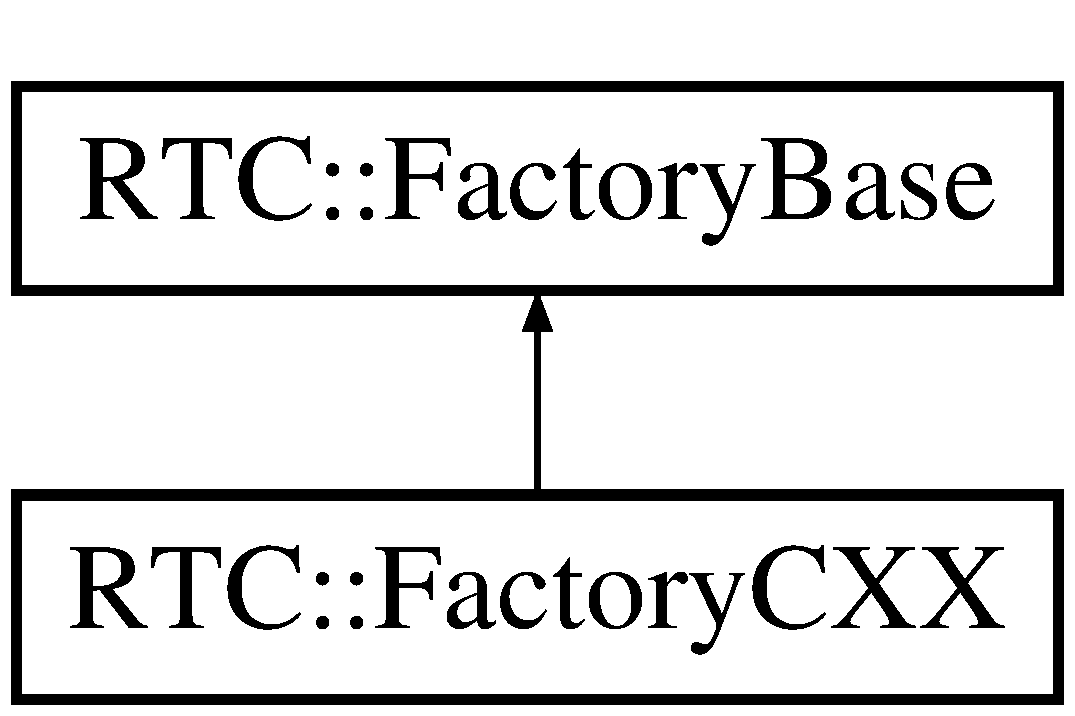
\includegraphics[height=2cm]{classRTC_1_1FactoryCXX}
\end{center}
\end{figure}
\subsection*{Public メソッド}
\begin{DoxyCompactItemize}
\item 
{\bf FactoryCXX} (const {\bf coil::Properties} \&profile, {\bf RtcNewFunc} new\_\-func, {\bf RtcDeleteFunc} delete\_\-func, {\bf NumberingPolicy} $\ast$policy=new {\bf DefaultNumberingPolicy}())
\begin{DoxyCompactList}\small\item\em コンストラクタ \item\end{DoxyCompactList}\item 
virtual {\bf $\sim$FactoryCXX} ()
\item 
virtual {\bf RTObject\_\-impl} $\ast$ {\bf create} ({\bf Manager} $\ast$mgr)
\begin{DoxyCompactList}\small\item\em コンポーネントの生成 \item\end{DoxyCompactList}\item 
virtual void {\bf destroy} ({\bf RTObject\_\-impl} $\ast$comp)
\begin{DoxyCompactList}\small\item\em コンポーネントの破棄 \item\end{DoxyCompactList}\end{DoxyCompactItemize}
\subsection*{Protected 変数}
\begin{DoxyCompactItemize}
\item 
{\bf RtcNewFunc} {\bf m\_\-New}
\begin{DoxyCompactList}\small\item\em コンポーネントオブジェクト生成関数へのポインタ \item\end{DoxyCompactList}\item 
{\bf RtcDeleteFunc} {\bf m\_\-Delete}
\begin{DoxyCompactList}\small\item\em コンポーネントオブジェクト破棄関数へのポインタ \item\end{DoxyCompactList}\item 
{\bf NumberingPolicy} $\ast$ {\bf m\_\-policy}
\begin{DoxyCompactList}\small\item\em コンポーネント生成時の命名ポリシー \item\end{DoxyCompactList}\end{DoxyCompactItemize}


\subsection{説明}
\doxyref{FactoryCXX}{p.}{classRTC_1_1FactoryCXX} クラス. C++用コンポーネントファクトリクラス。

\begin{DoxySince}{から}
0.2.0 
\end{DoxySince}


\subsection{コンストラクタとデストラクタ}
\index{RTC::FactoryCXX@{RTC::FactoryCXX}!FactoryCXX@{FactoryCXX}}
\index{FactoryCXX@{FactoryCXX}!RTC::FactoryCXX@{RTC::FactoryCXX}}
\subsubsection[{FactoryCXX}]{\setlength{\rightskip}{0pt plus 5cm}RTC::FactoryCXX::FactoryCXX (const {\bf coil::Properties} \& {\em profile}, \/  {\bf RtcNewFunc} {\em new\_\-func}, \/  {\bf RtcDeleteFunc} {\em delete\_\-func}, \/  {\bf NumberingPolicy} $\ast$ {\em policy} = {\ttfamily new~{\bf DefaultNumberingPolicy}()})}\label{classRTC_1_1FactoryCXX_a899ed96d9e5525f8dbd21e6306dd2311}


コンストラクタ 

コンストラクタ。 プロファイル、生成関数へのポインタ、破棄関数へのポインタ、 コンポーネント生成時の命名ポリシーを引数に取り、 C++ で実装されたコンポーネントのファクトリクラスを生成する。


\begin{DoxyParams}{引数}
\item[{\em profile}]コンポーネントのプロファイル \item[{\em new\_\-func}]コンポーネントの生成関数へのポインタ \item[{\em delete\_\-func}]コンポーネントの破棄関数へのポインタ \item[{\em policy}]コンポーネント生成時の命名ポリシー (デフォルト値:\doxyref{DefaultNumberingPolicy}{p.}{classDefaultNumberingPolicy}) \end{DoxyParams}
\index{RTC::FactoryCXX@{RTC::FactoryCXX}!$\sim$FactoryCXX@{$\sim$FactoryCXX}}
\index{$\sim$FactoryCXX@{$\sim$FactoryCXX}!RTC::FactoryCXX@{RTC::FactoryCXX}}
\subsubsection[{$\sim$FactoryCXX}]{\setlength{\rightskip}{0pt plus 5cm}virtual RTC::FactoryCXX::$\sim$FactoryCXX ()\hspace{0.3cm}{\ttfamily  [inline, virtual]}}\label{classRTC_1_1FactoryCXX_aac5ae8d77d40e9be05e5b1706e4a0137}


参照先 m\_\-policy.



\subsection{関数}
\index{RTC::FactoryCXX@{RTC::FactoryCXX}!create@{create}}
\index{create@{create}!RTC::FactoryCXX@{RTC::FactoryCXX}}
\subsubsection[{create}]{\setlength{\rightskip}{0pt plus 5cm}virtual {\bf RTObject\_\-impl}$\ast$ RTC::FactoryCXX::create ({\bf Manager} $\ast$ {\em mgr})\hspace{0.3cm}{\ttfamily  [virtual]}}\label{classRTC_1_1FactoryCXX_adf709b76b21aefe81338d9b885dcdcbe}


コンポーネントの生成 

RT-\/Component のインスタンスを生成する。


\begin{DoxyParams}{引数}
\item[{\em mgr}]マネージャオブジェクト\end{DoxyParams}
\begin{DoxyReturn}{戻り値}
生成したコンポーネント 
\end{DoxyReturn}


{\bf RTC::FactoryBase} \doxyref{}{p.}{classRTC_1_1FactoryBase_a08c22a5849ae192e442ce11754fb0be7}を実装しています。

\index{RTC::FactoryCXX@{RTC::FactoryCXX}!destroy@{destroy}}
\index{destroy@{destroy}!RTC::FactoryCXX@{RTC::FactoryCXX}}
\subsubsection[{destroy}]{\setlength{\rightskip}{0pt plus 5cm}virtual void RTC::FactoryCXX::destroy ({\bf RTObject\_\-impl} $\ast$ {\em comp})\hspace{0.3cm}{\ttfamily  [virtual]}}\label{classRTC_1_1FactoryCXX_a627c4dd3b5686d4df13a39c2a481c8e4}


コンポーネントの破棄 

RT-\/Component のインスタンスを破棄する。


\begin{DoxyParams}{引数}
\item[{\em comp}]破棄対象 RT-\/Component \end{DoxyParams}


{\bf RTC::FactoryBase} \doxyref{}{p.}{classRTC_1_1FactoryBase_aa7cb36bdcc0c8debba468b064ce03e7e}を実装しています。



\subsection{変数}
\index{RTC::FactoryCXX@{RTC::FactoryCXX}!m\_\-Delete@{m\_\-Delete}}
\index{m\_\-Delete@{m\_\-Delete}!RTC::FactoryCXX@{RTC::FactoryCXX}}
\subsubsection[{m\_\-Delete}]{\setlength{\rightskip}{0pt plus 5cm}{\bf RtcDeleteFunc} {\bf RTC::FactoryCXX::m\_\-Delete}\hspace{0.3cm}{\ttfamily  [protected]}}\label{classRTC_1_1FactoryCXX_abb2914e846bc84a822189bdd290ddbab}


コンポーネントオブジェクト破棄関数へのポインタ 

\index{RTC::FactoryCXX@{RTC::FactoryCXX}!m\_\-New@{m\_\-New}}
\index{m\_\-New@{m\_\-New}!RTC::FactoryCXX@{RTC::FactoryCXX}}
\subsubsection[{m\_\-New}]{\setlength{\rightskip}{0pt plus 5cm}{\bf RtcNewFunc} {\bf RTC::FactoryCXX::m\_\-New}\hspace{0.3cm}{\ttfamily  [protected]}}\label{classRTC_1_1FactoryCXX_a2f437b41029d2a66893b3d49db0a0808}


コンポーネントオブジェクト生成関数へのポインタ 

\index{RTC::FactoryCXX@{RTC::FactoryCXX}!m\_\-policy@{m\_\-policy}}
\index{m\_\-policy@{m\_\-policy}!RTC::FactoryCXX@{RTC::FactoryCXX}}
\subsubsection[{m\_\-policy}]{\setlength{\rightskip}{0pt plus 5cm}{\bf NumberingPolicy}$\ast$ {\bf RTC::FactoryCXX::m\_\-policy}\hspace{0.3cm}{\ttfamily  [protected]}}\label{classRTC_1_1FactoryCXX_a5114c456980db9cd6645353628fb20bd}


コンポーネント生成時の命名ポリシー 



参照元 $\sim$FactoryCXX().


\section{クラス RTC::Manager::FactoryPredicate}
\label{classRTC_1_1Manager_1_1FactoryPredicate}\index{RTC::Manager::FactoryPredicate@{RTC::Manager::FactoryPredicate}}


{\ttfamily \#include $<$Manager.h$>$}

\subsection*{Public メソッド}
\begin{DoxyCompactItemize}
\item 
{\bf FactoryPredicate} (const char $\ast$imple\_\-id)
\item 
{\bf FactoryPredicate} (const {\bf coil::Properties} \&prop)
\item 
{\bf FactoryPredicate} ({\bf FactoryBase} $\ast$factory)
\item 
bool {\bf operator()} ({\bf FactoryBase} $\ast$factory)
\end{DoxyCompactItemize}


\subsection{コンストラクタとデストラクタ}
\index{RTC::Manager::FactoryPredicate@{RTC::Manager::FactoryPredicate}!FactoryPredicate@{FactoryPredicate}}
\index{FactoryPredicate@{FactoryPredicate}!RTC::Manager::FactoryPredicate@{RTC::Manager::FactoryPredicate}}
\subsubsection[{FactoryPredicate}]{\setlength{\rightskip}{0pt plus 5cm}RTC::Manager::FactoryPredicate::FactoryPredicate (const char $\ast$ {\em imple\_\-id})\hspace{0.3cm}{\ttfamily  [inline]}}\label{classRTC_1_1Manager_1_1FactoryPredicate_a1d0eea85745cc10f3fd32d80e6743264}
\index{RTC::Manager::FactoryPredicate@{RTC::Manager::FactoryPredicate}!FactoryPredicate@{FactoryPredicate}}
\index{FactoryPredicate@{FactoryPredicate}!RTC::Manager::FactoryPredicate@{RTC::Manager::FactoryPredicate}}
\subsubsection[{FactoryPredicate}]{\setlength{\rightskip}{0pt plus 5cm}RTC::Manager::FactoryPredicate::FactoryPredicate (const {\bf coil::Properties} \& {\em prop})\hspace{0.3cm}{\ttfamily  [inline]}}\label{classRTC_1_1Manager_1_1FactoryPredicate_aecd5e7c53b169caf67229ac3025bce4e}
\index{RTC::Manager::FactoryPredicate@{RTC::Manager::FactoryPredicate}!FactoryPredicate@{FactoryPredicate}}
\index{FactoryPredicate@{FactoryPredicate}!RTC::Manager::FactoryPredicate@{RTC::Manager::FactoryPredicate}}
\subsubsection[{FactoryPredicate}]{\setlength{\rightskip}{0pt plus 5cm}RTC::Manager::FactoryPredicate::FactoryPredicate ({\bf FactoryBase} $\ast$ {\em factory})\hspace{0.3cm}{\ttfamily  [inline]}}\label{classRTC_1_1Manager_1_1FactoryPredicate_a0727638df0c5a930f20c805ccc660a6e}


\subsection{関数}
\index{RTC::Manager::FactoryPredicate@{RTC::Manager::FactoryPredicate}!operator()@{operator()}}
\index{operator()@{operator()}!RTC::Manager::FactoryPredicate@{RTC::Manager::FactoryPredicate}}
\subsubsection[{operator()}]{\setlength{\rightskip}{0pt plus 5cm}bool RTC::Manager::FactoryPredicate::operator() ({\bf FactoryBase} $\ast$ {\em factory})\hspace{0.3cm}{\ttfamily  [inline]}}\label{classRTC_1_1Manager_1_1FactoryPredicate_a292a83f4047f23485d4529a3b3e0591d}


参照先 RTC::FactoryBase::profile().


\section{構造体 RTC::ModuleManager::FileNotFound}
\label{structRTC_1_1ModuleManager_1_1FileNotFound}\index{RTC::ModuleManager::FileNotFound@{RTC::ModuleManager::FileNotFound}}


指定ファイル不明例外処理用構造体  




{\ttfamily \#include $<$ModuleManager.h$>$}

RTC::ModuleManager::FileNotFoundに対する継承グラフ\begin{figure}[H]
\begin{center}
\leavevmode
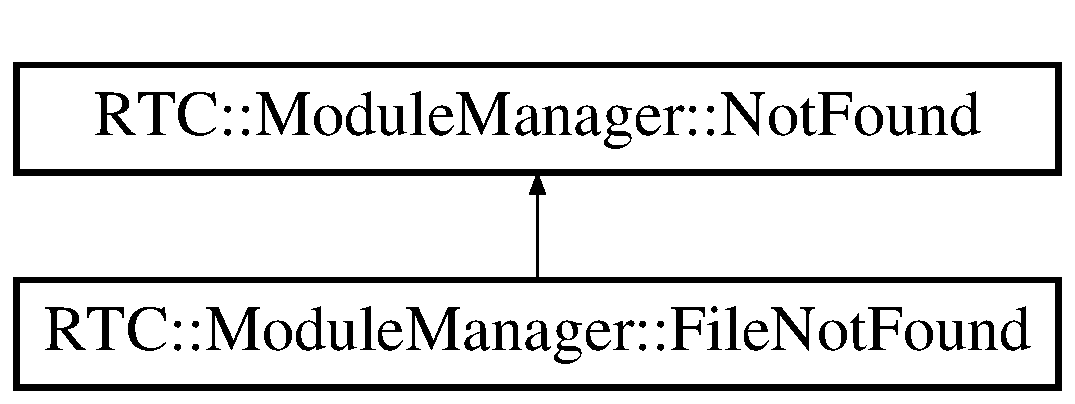
\includegraphics[height=2cm]{structRTC_1_1ModuleManager_1_1FileNotFound}
\end{center}
\end{figure}
\subsection*{Public メソッド}
\begin{DoxyCompactItemize}
\item 
{\bf FileNotFound} (const std::string \&\_\-name)
\end{DoxyCompactItemize}


\subsection{説明}
指定ファイル不明例外処理用構造体 

\subsection{コンストラクタとデストラクタ}
\index{RTC::ModuleManager::FileNotFound@{RTC::ModuleManager::FileNotFound}!FileNotFound@{FileNotFound}}
\index{FileNotFound@{FileNotFound}!RTC::ModuleManager::FileNotFound@{RTC::ModuleManager::FileNotFound}}
\subsubsection[{FileNotFound}]{\setlength{\rightskip}{0pt plus 5cm}RTC::ModuleManager::FileNotFound::FileNotFound (const std::string \& {\em \_\-name})\hspace{0.3cm}{\ttfamily  [inline]}}\label{structRTC_1_1ModuleManager_1_1FileNotFound_a698b99562aac6bba9516f645d7ea4f48}

\section{構造体 RTC::Manager::Finalized}
\label{structRTC_1_1Manager_1_1Finalized}\index{RTC::Manager::Finalized@{RTC::Manager::Finalized}}


{\ttfamily \#include $<$Manager.h$>$}

\subsection*{Public 変数}
\begin{DoxyCompactItemize}
\item 
{\bf Mutex} {\bf mutex}
\item 
std::vector$<$ {\bf RTObject\_\-impl} $\ast$ $>$ {\bf comps}
\end{DoxyCompactItemize}


\subsection{変数}
\index{RTC::Manager::Finalized@{RTC::Manager::Finalized}!comps@{comps}}
\index{comps@{comps}!RTC::Manager::Finalized@{RTC::Manager::Finalized}}
\subsubsection[{comps}]{\setlength{\rightskip}{0pt plus 5cm}std::vector$<${\bf RTObject\_\-impl}$\ast$$>$ {\bf RTC::Manager::Finalized::comps}}\label{structRTC_1_1Manager_1_1Finalized_add3526b268ef3d0fd43c8603dbda9aa9}
\index{RTC::Manager::Finalized@{RTC::Manager::Finalized}!mutex@{mutex}}
\index{mutex@{mutex}!RTC::Manager::Finalized@{RTC::Manager::Finalized}}
\subsubsection[{mutex}]{\setlength{\rightskip}{0pt plus 5cm}{\bf Mutex} {\bf RTC::Manager::Finalized::mutex}}\label{structRTC_1_1Manager_1_1Finalized_a1d6c77f44b768021ad3f9fe06f09f590}

\section{構造体 RTC::PeriodicExecutionContext::find\_\-comp}
\label{structRTC_1_1PeriodicExecutionContext_1_1find__comp}\index{RTC::PeriodicExecutionContext::find\_\-comp@{RTC::PeriodicExecutionContext::find\_\-comp}}


コンポーネント検索用ファンクタ  




{\ttfamily \#include $<$PeriodicExecutionContext.h$>$}

\subsection*{Public メソッド}
\begin{DoxyCompactItemize}
\item 
{\bf find\_\-comp} (LightweightRTObject\_\-ptr comp)
\item 
bool {\bf operator()} ({\bf Comp} \&comp)
\end{DoxyCompactItemize}
\subsection*{Public 変数}
\begin{DoxyCompactItemize}
\item 
LightweightRTObject\_\-var {\bf m\_\-comp}
\end{DoxyCompactItemize}


\subsection{説明}
コンポーネント検索用ファンクタ 

\subsection{コンストラクタとデストラクタ}
\index{RTC::PeriodicExecutionContext::find\_\-comp@{RTC::PeriodicExecutionContext::find\_\-comp}!find\_\-comp@{find\_\-comp}}
\index{find\_\-comp@{find\_\-comp}!RTC::PeriodicExecutionContext::find_comp@{RTC::PeriodicExecutionContext::find\_\-comp}}
\subsubsection[{find\_\-comp}]{\setlength{\rightskip}{0pt plus 5cm}RTC::PeriodicExecutionContext::find\_\-comp::find\_\-comp (LightweightRTObject\_\-ptr {\em comp})\hspace{0.3cm}{\ttfamily  [inline]}}\label{structRTC_1_1PeriodicExecutionContext_1_1find__comp_ad122d50fe656d3cfa2d0a32a6a05b950}


\subsection{関数}
\index{RTC::PeriodicExecutionContext::find\_\-comp@{RTC::PeriodicExecutionContext::find\_\-comp}!operator()@{operator()}}
\index{operator()@{operator()}!RTC::PeriodicExecutionContext::find_comp@{RTC::PeriodicExecutionContext::find\_\-comp}}
\subsubsection[{operator()}]{\setlength{\rightskip}{0pt plus 5cm}bool RTC::PeriodicExecutionContext::find\_\-comp::operator() ({\bf Comp} \& {\em comp})\hspace{0.3cm}{\ttfamily  [inline]}}\label{structRTC_1_1PeriodicExecutionContext_1_1find__comp_ab415ecce5cdd2e5bb9893bcc406ecdad}


参照先 RTC::PeriodicExecutionContext::Comp::\_\-ref, と m\_\-comp.



\subsection{変数}
\index{RTC::PeriodicExecutionContext::find\_\-comp@{RTC::PeriodicExecutionContext::find\_\-comp}!m\_\-comp@{m\_\-comp}}
\index{m\_\-comp@{m\_\-comp}!RTC::PeriodicExecutionContext::find_comp@{RTC::PeriodicExecutionContext::find\_\-comp}}
\subsubsection[{m\_\-comp}]{\setlength{\rightskip}{0pt plus 5cm}LightweightRTObject\_\-var {\bf RTC::PeriodicExecutionContext::find\_\-comp::m\_\-comp}}\label{structRTC_1_1PeriodicExecutionContext_1_1find__comp_acb89128f9276fad13db229fc5156e840}


参照元 operator()().


\section{構造体 RTC::PortBase::find\_\-conn\_\-id}
\label{structRTC_1_1PortBase_1_1find__conn__id}\index{RTC::PortBase::find\_\-conn\_\-id@{RTC::PortBase::find\_\-conn\_\-id}}


id を持つ ConnectorProfile を探す Functor  




{\ttfamily \#include $<$PortBase.h$>$}

\subsection*{Public メソッド}
\begin{DoxyCompactItemize}
\item 
{\bf find\_\-conn\_\-id} (const char $\ast$id)
\item 
bool {\bf operator()} (const ConnectorProfile \&cprof)
\end{DoxyCompactItemize}
\subsection*{Public 変数}
\begin{DoxyCompactItemize}
\item 
std::string {\bf m\_\-id}
\end{DoxyCompactItemize}


\subsection{説明}
id を持つ ConnectorProfile を探す Functor 

\subsection{コンストラクタとデストラクタ}
\index{RTC::PortBase::find\_\-conn\_\-id@{RTC::PortBase::find\_\-conn\_\-id}!find\_\-conn\_\-id@{find\_\-conn\_\-id}}
\index{find\_\-conn\_\-id@{find\_\-conn\_\-id}!RTC::PortBase::find_conn_id@{RTC::PortBase::find\_\-conn\_\-id}}
\subsubsection[{find\_\-conn\_\-id}]{\setlength{\rightskip}{0pt plus 5cm}RTC::PortBase::find\_\-conn\_\-id::find\_\-conn\_\-id (const char $\ast$ {\em id})\hspace{0.3cm}{\ttfamily  [inline]}}\label{structRTC_1_1PortBase_1_1find__conn__id_a0c5e57c7f8b1bf719135c52eed175223}


\subsection{関数}
\index{RTC::PortBase::find\_\-conn\_\-id@{RTC::PortBase::find\_\-conn\_\-id}!operator()@{operator()}}
\index{operator()@{operator()}!RTC::PortBase::find_conn_id@{RTC::PortBase::find\_\-conn\_\-id}}
\subsubsection[{operator()}]{\setlength{\rightskip}{0pt plus 5cm}bool RTC::PortBase::find\_\-conn\_\-id::operator() (const ConnectorProfile \& {\em cprof})\hspace{0.3cm}{\ttfamily  [inline]}}\label{structRTC_1_1PortBase_1_1find__conn__id_ae6b3bf71f8ddb52f0be1c383e4fadbab}


参照先 m\_\-id.



\subsection{変数}
\index{RTC::PortBase::find\_\-conn\_\-id@{RTC::PortBase::find\_\-conn\_\-id}!m\_\-id@{m\_\-id}}
\index{m\_\-id@{m\_\-id}!RTC::PortBase::find_conn_id@{RTC::PortBase::find\_\-conn\_\-id}}
\subsubsection[{m\_\-id}]{\setlength{\rightskip}{0pt plus 5cm}std::string {\bf RTC::PortBase::find\_\-conn\_\-id::m\_\-id}}\label{structRTC_1_1PortBase_1_1find__conn__id_afae0272a2a0305bcba9677266e0871d7}


参照元 operator()().


\section{RTC::PortBase::find\_\-interface Struct Reference}
\label{structRTC_1_1PortBase_1_1find__interface}\index{RTC::PortBase::find\_\-interface@{RTC::PortBase::find\_\-interface}}


Functor to find interface from name and polarity.  




{\ttfamily \#include $<$PortBase.h$>$}

\subsection*{Public Member Functions}
\begin{DoxyCompactItemize}
\item 
{\bf find\_\-interface} (const char $\ast$name, PortInterfacePolarity pol)
\item 
bool {\bf operator()} (const PortInterfaceProfile \&prof)
\end{DoxyCompactItemize}
\subsection*{Public Attributes}
\begin{DoxyCompactItemize}
\item 
std::string {\bf m\_\-name}
\item 
PortInterfacePolarity {\bf m\_\-pol}
\end{DoxyCompactItemize}


\subsection{Detailed Description}
Functor to find interface from name and polarity. 

\subsection{Constructor \& Destructor Documentation}
\index{RTC::PortBase::find\_\-interface@{RTC::PortBase::find\_\-interface}!find\_\-interface@{find\_\-interface}}
\index{find\_\-interface@{find\_\-interface}!RTC::PortBase::find_interface@{RTC::PortBase::find\_\-interface}}
\subsubsection[{find\_\-interface}]{\setlength{\rightskip}{0pt plus 5cm}RTC::PortBase::find\_\-interface::find\_\-interface (const char $\ast$ {\em name}, \/  PortInterfacePolarity {\em pol})\hspace{0.3cm}{\ttfamily  [inline]}}\label{structRTC_1_1PortBase_1_1find__interface_ace212b36529cbb4723654674caba86d3}


\subsection{Member Function Documentation}
\index{RTC::PortBase::find\_\-interface@{RTC::PortBase::find\_\-interface}!operator()@{operator()}}
\index{operator()@{operator()}!RTC::PortBase::find_interface@{RTC::PortBase::find\_\-interface}}
\subsubsection[{operator()}]{\setlength{\rightskip}{0pt plus 5cm}bool RTC::PortBase::find\_\-interface::operator() (const PortInterfaceProfile \& {\em prof})\hspace{0.3cm}{\ttfamily  [inline]}}\label{structRTC_1_1PortBase_1_1find__interface_a68d0b425d5ba86e6d118b0bb088a94c4}


References m\_\-name, and m\_\-pol.



\subsection{Member Data Documentation}
\index{RTC::PortBase::find\_\-interface@{RTC::PortBase::find\_\-interface}!m\_\-name@{m\_\-name}}
\index{m\_\-name@{m\_\-name}!RTC::PortBase::find_interface@{RTC::PortBase::find\_\-interface}}
\subsubsection[{m\_\-name}]{\setlength{\rightskip}{0pt plus 5cm}std::string {\bf RTC::PortBase::find\_\-interface::m\_\-name}}\label{structRTC_1_1PortBase_1_1find__interface_a6a60bc810b70be94985e0e912fb66efe}


Referenced by operator()().

\index{RTC::PortBase::find\_\-interface@{RTC::PortBase::find\_\-interface}!m\_\-pol@{m\_\-pol}}
\index{m\_\-pol@{m\_\-pol}!RTC::PortBase::find_interface@{RTC::PortBase::find\_\-interface}}
\subsubsection[{m\_\-pol}]{\setlength{\rightskip}{0pt plus 5cm}PortInterfacePolarity {\bf RTC::PortBase::find\_\-interface::m\_\-pol}}\label{structRTC_1_1PortBase_1_1find__interface_a762775406f1eefad0406aecbfce55d98}


Referenced by operator()().


\section{RTC::PeriodicExecutionContext::find\_\-participant Class Reference}
\label{classRTC_1_1PeriodicExecutionContext_1_1find__participant}\index{RTC::PeriodicExecutionContext::find\_\-participant@{RTC::PeriodicExecutionContext::find\_\-participant}}


{\ttfamily \#include $<$PeriodicExecutionContext.h$>$}

\subsection*{Public Member Functions}
\begin{DoxyCompactItemize}
\item 
{\bf find\_\-participant} (RTObject\_\-ptr comp)
\item 
bool {\bf operator()} (RTObject\_\-ptr comp)
\end{DoxyCompactItemize}


\subsection{Constructor \& Destructor Documentation}
\index{RTC::PeriodicExecutionContext::find\_\-participant@{RTC::PeriodicExecutionContext::find\_\-participant}!find\_\-participant@{find\_\-participant}}
\index{find\_\-participant@{find\_\-participant}!RTC::PeriodicExecutionContext::find_participant@{RTC::PeriodicExecutionContext::find\_\-participant}}
\subsubsection[{find\_\-participant}]{\setlength{\rightskip}{0pt plus 5cm}RTC::PeriodicExecutionContext::find\_\-participant::find\_\-participant (RTObject\_\-ptr {\em comp})\hspace{0.3cm}{\ttfamily  [inline]}}\label{classRTC_1_1PeriodicExecutionContext_1_1find__participant_a9a17ee3de46809d56fa740db0de63b95}


\subsection{Member Function Documentation}
\index{RTC::PeriodicExecutionContext::find\_\-participant@{RTC::PeriodicExecutionContext::find\_\-participant}!operator()@{operator()}}
\index{operator()@{operator()}!RTC::PeriodicExecutionContext::find_participant@{RTC::PeriodicExecutionContext::find\_\-participant}}
\subsubsection[{operator()}]{\setlength{\rightskip}{0pt plus 5cm}bool RTC::PeriodicExecutionContext::find\_\-participant::operator() (RTObject\_\-ptr {\em comp})\hspace{0.3cm}{\ttfamily  [inline]}}\label{classRTC_1_1PeriodicExecutionContext_1_1find__participant_a8ff35c40d5e9998fd9516e675486f834}

\section{RTC::PortBase::find\_\-port\_\-ref Struct Reference}
\label{structRTC_1_1PortBase_1_1find__port__ref}\index{RTC::PortBase::find\_\-port\_\-ref@{RTC::PortBase::find\_\-port\_\-ref}}


Functor to find the object reference that is identical port\_\-ref.  




{\ttfamily \#include $<$PortBase.h$>$}

\subsection*{Public Member Functions}
\begin{DoxyCompactItemize}
\item 
{\bf find\_\-port\_\-ref} (PortService\_\-ptr port\_\-ref)
\item 
bool {\bf operator()} (PortService\_\-ptr port\_\-ref)
\end{DoxyCompactItemize}
\subsection*{Public Attributes}
\begin{DoxyCompactItemize}
\item 
PortService\_\-ptr {\bf m\_\-port}
\end{DoxyCompactItemize}


\subsection{Detailed Description}
Functor to find the object reference that is identical port\_\-ref. 

\subsection{Constructor \& Destructor Documentation}
\index{RTC::PortBase::find\_\-port\_\-ref@{RTC::PortBase::find\_\-port\_\-ref}!find\_\-port\_\-ref@{find\_\-port\_\-ref}}
\index{find\_\-port\_\-ref@{find\_\-port\_\-ref}!RTC::PortBase::find_port_ref@{RTC::PortBase::find\_\-port\_\-ref}}
\subsubsection[{find\_\-port\_\-ref}]{\setlength{\rightskip}{0pt plus 5cm}RTC::PortBase::find\_\-port\_\-ref::find\_\-port\_\-ref (PortService\_\-ptr {\em port\_\-ref})\hspace{0.3cm}{\ttfamily  [inline]}}\label{structRTC_1_1PortBase_1_1find__port__ref_a67c224b2a7b154dd2654f759576fea52}


\subsection{Member Function Documentation}
\index{RTC::PortBase::find\_\-port\_\-ref@{RTC::PortBase::find\_\-port\_\-ref}!operator()@{operator()}}
\index{operator()@{operator()}!RTC::PortBase::find_port_ref@{RTC::PortBase::find\_\-port\_\-ref}}
\subsubsection[{operator()}]{\setlength{\rightskip}{0pt plus 5cm}bool RTC::PortBase::find\_\-port\_\-ref::operator() (PortService\_\-ptr {\em port\_\-ref})\hspace{0.3cm}{\ttfamily  [inline]}}\label{structRTC_1_1PortBase_1_1find__port__ref_a967c45942757ed5aabf768f68f5d7d89}


References m\_\-port.



\subsection{Member Data Documentation}
\index{RTC::PortBase::find\_\-port\_\-ref@{RTC::PortBase::find\_\-port\_\-ref}!m\_\-port@{m\_\-port}}
\index{m\_\-port@{m\_\-port}!RTC::PortBase::find_port_ref@{RTC::PortBase::find\_\-port\_\-ref}}
\subsubsection[{m\_\-port}]{\setlength{\rightskip}{0pt plus 5cm}PortService\_\-ptr {\bf RTC::PortBase::find\_\-port\_\-ref::m\_\-port}}\label{structRTC_1_1PortBase_1_1find__port__ref_a83a1c3cd2fb4a1a5986383e1836b6ec5}


Referenced by operator()().


\section{クラス coil::GetOpt}
\label{classcoil_1_1GetOpt}\index{coil::GetOpt@{coil::GetOpt}}


\doxyref{GetOpt}{p.}{classcoil_1_1GetOpt} クラス.  




{\ttfamily \#include $<$OS.h$>$}

\subsection*{Public メソッド}
\begin{DoxyCompactItemize}
\item 
{\bf GetOpt} (int argc, char $\ast$const argv[$\,$], const char $\ast$opt, int flag)
\begin{DoxyCompactList}\small\item\em コンストラクタ \item\end{DoxyCompactList}\item 
{\bf $\sim$GetOpt} ()
\begin{DoxyCompactList}\small\item\em デストラクタ \item\end{DoxyCompactList}\item 
int {\bf operator()} ()
\begin{DoxyCompactList}\small\item\em コマンドライン引数解析 \item\end{DoxyCompactList}\end{DoxyCompactItemize}
\subsection*{Public 変数}
\begin{DoxyCompactItemize}
\item 
char $\ast$ {\bf optarg}
\item 
int {\bf optind}
\begin{DoxyCompactList}\small\item\em オプション引数 \item\end{DoxyCompactList}\item 
int {\bf opterr}
\begin{DoxyCompactList}\small\item\em 処理対象引数 \item\end{DoxyCompactList}\item 
int {\bf optopt}
\begin{DoxyCompactList}\small\item\em エラー表示 0:抑止、1:表示 \item\end{DoxyCompactList}\end{DoxyCompactItemize}


\subsection{説明}
\doxyref{GetOpt}{p.}{classcoil_1_1GetOpt} クラス. 

\subsection{コンストラクタとデストラクタ}
\index{coil::GetOpt@{coil::GetOpt}!GetOpt@{GetOpt}}
\index{GetOpt@{GetOpt}!coil::GetOpt@{coil::GetOpt}}
\subsubsection[{GetOpt}]{\setlength{\rightskip}{0pt plus 5cm}coil::GetOpt::GetOpt (int {\em argc}, \/  char $\ast$const  {\em argv}[$\,$], \/  const char $\ast$ {\em opt}, \/  int {\em flag})\hspace{0.3cm}{\ttfamily  [inline]}}\label{classcoil_1_1GetOpt_ac5d327f254117a66c9f2f1a60d02f2fd}


コンストラクタ 

コンストラクタ。


\begin{DoxyParams}{引数}
\item[{\em name}]オブジェクト名 \end{DoxyParams}


参照先 optind.

\index{coil::GetOpt@{coil::GetOpt}!$\sim$GetOpt@{$\sim$GetOpt}}
\index{$\sim$GetOpt@{$\sim$GetOpt}!coil::GetOpt@{coil::GetOpt}}
\subsubsection[{$\sim$GetOpt}]{\setlength{\rightskip}{0pt plus 5cm}coil::GetOpt::$\sim$GetOpt ()\hspace{0.3cm}{\ttfamily  [inline]}}\label{classcoil_1_1GetOpt_ac72f5662f12ddac40609a91d7ef91dca}


デストラクタ 

デストラクタ。 

参照先 optind.



\subsection{関数}
\index{coil::GetOpt@{coil::GetOpt}!operator()@{operator()}}
\index{operator()@{operator()}!coil::GetOpt@{coil::GetOpt}}
\subsubsection[{operator()}]{\setlength{\rightskip}{0pt plus 5cm}int coil::GetOpt::operator() ()\hspace{0.3cm}{\ttfamily  [inline]}}\label{classcoil_1_1GetOpt_aeccfe44e8e4cf01a3eb105f06414e3f8}


コマンドライン引数解析 

コマンドライン引数を解析する。

\begin{DoxyReturn}{戻り値}
解析結果 
\end{DoxyReturn}


参照先 optarg, opterr, optind, と optopt.



\subsection{変数}
\index{coil::GetOpt@{coil::GetOpt}!optarg@{optarg}}
\index{optarg@{optarg}!coil::GetOpt@{coil::GetOpt}}
\subsubsection[{optarg}]{\setlength{\rightskip}{0pt plus 5cm}char$\ast$ {\bf coil::GetOpt::optarg}}\label{classcoil_1_1GetOpt_ab737d20597f45c203ee94149602fd76e}


参照元 operator()().

\index{coil::GetOpt@{coil::GetOpt}!opterr@{opterr}}
\index{opterr@{opterr}!coil::GetOpt@{coil::GetOpt}}
\subsubsection[{opterr}]{\setlength{\rightskip}{0pt plus 5cm}int {\bf coil::GetOpt::opterr}}\label{classcoil_1_1GetOpt_ad0c8937327497c149a3e9fc2b8848849}


処理対象引数 



参照元 operator()().

\index{coil::GetOpt@{coil::GetOpt}!optind@{optind}}
\index{optind@{optind}!coil::GetOpt@{coil::GetOpt}}
\subsubsection[{optind}]{\setlength{\rightskip}{0pt plus 5cm}int {\bf coil::GetOpt::optind}}\label{classcoil_1_1GetOpt_a65e9137c10e3f5d0558b1a2581314ac2}


オプション引数 



参照元 GetOpt(), operator()(), と $\sim$GetOpt().

\index{coil::GetOpt@{coil::GetOpt}!optopt@{optopt}}
\index{optopt@{optopt}!coil::GetOpt@{coil::GetOpt}}
\subsubsection[{optopt}]{\setlength{\rightskip}{0pt plus 5cm}int {\bf coil::GetOpt::optopt}}\label{classcoil_1_1GetOpt_a6b068abe70b88844f85a2eda5855e29d}


エラー表示 0:抑止、1:表示 



参照元 operator()().


\section{クラス テンプレート coil::GlobalFactory$<$ AbstractClass, Identifier, Compare, Creator, Destructor $>$}
\label{classcoil_1_1GlobalFactory}\index{coil::GlobalFactory@{coil::GlobalFactory}}


\doxyref{GlobalFactory}{p.}{classcoil_1_1GlobalFactory} テンプレートクラス.  




{\ttfamily \#include $<$Factory.h$>$}

coil::GlobalFactory$<$ AbstractClass, Identifier, Compare, Creator, Destructor $>$に対する継承グラフ\begin{figure}[H]
\begin{center}
\leavevmode
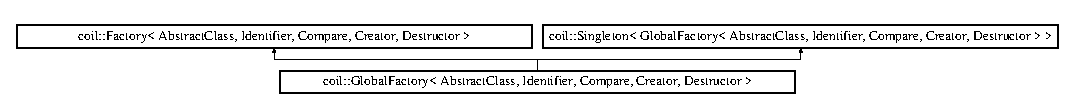
\includegraphics[height=1.03321cm]{classcoil_1_1GlobalFactory}
\end{center}
\end{figure}
\subsection*{フレンド}
\begin{DoxyCompactItemize}
\item 
class {\bf Singleton$<$ GlobalFactory $>$}
\end{DoxyCompactItemize}


\subsection{説明}
\subsubsection*{template$<$class AbstractClass, typename Identifier = std::string, typename Compare = std::less$<$Identifier$>$, typename Creator = AbstractClass$\ast$ ($\ast$)(), typename Destructor = void ($\ast$)(AbstractClass$\ast$\&)$>$ class coil::GlobalFactory$<$ AbstractClass, Identifier, Compare, Creator, Destructor $>$}

\doxyref{GlobalFactory}{p.}{classcoil_1_1GlobalFactory} テンプレートクラス. 

\subsection{フレンドと関連する関数}
\index{coil::GlobalFactory@{coil::GlobalFactory}!Singleton$<$ GlobalFactory $>$@{Singleton$<$ GlobalFactory $>$}}
\index{Singleton$<$ GlobalFactory $>$@{Singleton$<$ GlobalFactory $>$}!coil::GlobalFactory@{coil::GlobalFactory}}
\subsubsection[{Singleton$<$ GlobalFactory $>$}]{\setlength{\rightskip}{0pt plus 5cm}template$<$class AbstractClass , typename Identifier  = std::string, typename Compare  = std::less$<$Identifier$>$, typename Creator  = AbstractClass$\ast$ ($\ast$)(), typename Destructor  = void ($\ast$)(AbstractClass$\ast$\&)$>$ friend class {\bf Singleton}$<$ {\bf GlobalFactory} $>$\hspace{0.3cm}{\ttfamily  [friend]}}\label{classcoil_1_1GlobalFactory_a50b941f98f8514f15bdfa144d1b9ee3d}

\section{coil::Guard$<$ M $>$ Class Template Reference}
\label{classcoil_1_1Guard}\index{coil::Guard@{coil::Guard}}


\doxyref{Guard}{p.}{classcoil_1_1Guard} template class.  




{\ttfamily \#include $<$Guard.h$>$}

\subsection*{Public Member Functions}
\begin{DoxyCompactItemize}
\item 
{\bf Guard} (M \&mutex)
\begin{DoxyCompactList}\small\item\em Constructor. \item\end{DoxyCompactList}\item 
{\bf $\sim$Guard} ()
\begin{DoxyCompactList}\small\item\em Destructor. \item\end{DoxyCompactList}\end{DoxyCompactItemize}


\subsection{Detailed Description}
\subsubsection*{template$<$class M$>$ class coil::Guard$<$ M $>$}

\doxyref{Guard}{p.}{classcoil_1_1Guard} template class. 

\subsection{Constructor \& Destructor Documentation}
\index{coil::Guard@{coil::Guard}!Guard@{Guard}}
\index{Guard@{Guard}!coil::Guard@{coil::Guard}}
\subsubsection[{Guard}]{\setlength{\rightskip}{0pt plus 5cm}template$<$class M$>$ {\bf coil::Guard}$<$ M $>$::{\bf Guard} (M \& {\em mutex})\hspace{0.3cm}{\ttfamily  [inline]}}\label{classcoil_1_1Guard_acbb2bd38567b0a5a91ba1aa8c9f40a58}


Constructor. 

Constructor


\begin{DoxyParams}{Parameters}
\item[{\em mutex}]pthread \end{DoxyParams}
\index{coil::Guard@{coil::Guard}!$\sim$Guard@{$\sim$Guard}}
\index{$\sim$Guard@{$\sim$Guard}!coil::Guard@{coil::Guard}}
\subsubsection[{$\sim$Guard}]{\setlength{\rightskip}{0pt plus 5cm}template$<$class M$>$ {\bf coil::Guard}$<$ M $>$::$\sim${\bf Guard} ()\hspace{0.3cm}{\ttfamily  [inline]}}\label{classcoil_1_1Guard_a4865d0a7667cbcc9cc011319d4c09251}


Destructor. 

Destructor 
\section{CORBA\_\-Util::has\_\-nil$<$ T $>$ Struct Template Reference}
\label{structCORBA__Util_1_1has__nil}\index{CORBA\_\-Util::has\_\-nil@{CORBA\_\-Util::has\_\-nil}}


has nil traits class template  




{\ttfamily \#include $<$Typename.h$>$}

Inheritance diagram for CORBA\_\-Util::has\_\-nil$<$ T $>$:\begin{figure}[H]
\begin{center}
\leavevmode
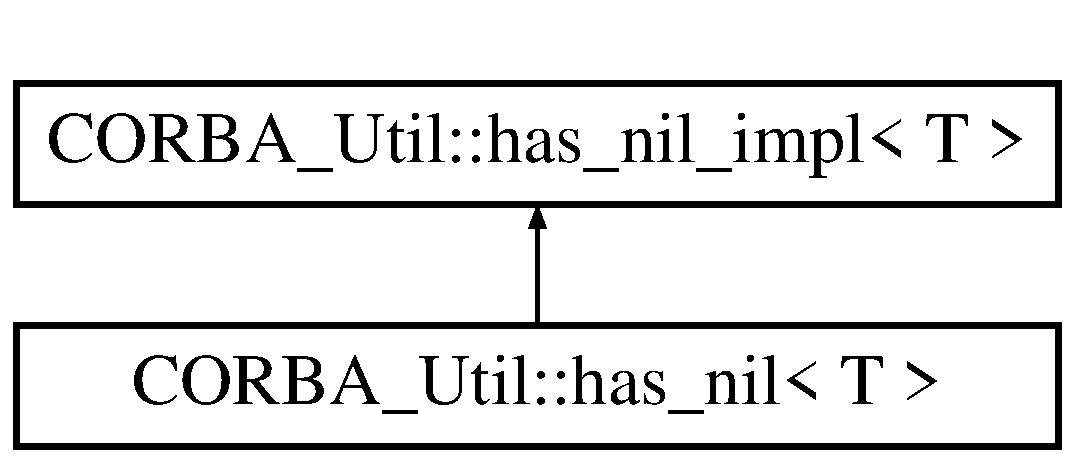
\includegraphics[height=2cm]{structCORBA__Util_1_1has__nil}
\end{center}
\end{figure}


\subsection{Detailed Description}
\subsubsection*{template$<$class T$>$ struct CORBA\_\-Util::has\_\-nil$<$ T $>$}

has nil traits class template T has \_\-nil() static function -\/$>$ value = true T has no \_\-nil() static function -\/$>$ value = false 
\section{構造体 テンプレート CORBA\_\-Util::has\_\-nil\_\-helper$<$ T, \_\-ptr\_\-type $>$}
\label{structCORBA__Util_1_1has__nil__helper}\index{CORBA\_\-Util::has\_\-nil\_\-helper@{CORBA\_\-Util::has\_\-nil\_\-helper}}


has nil helper  




{\ttfamily \#include $<$Typename.h$>$}

\subsection*{Public 型}
\begin{DoxyCompactItemize}
\item 
typedef void {\bf type}
\end{DoxyCompactItemize}


\subsection{説明}
\subsubsection*{template$<$class T, typename T:: \_\-ptr\_\-type$>$ struct CORBA\_\-Util::has\_\-nil\_\-helper$<$ T, \_\-ptr\_\-type $>$}

has nil helper typename T::\_\-ptr\_\-type ($\ast$)(void) matches \_\-nil() static member function 

\subsection{型定義}
\index{CORBA\_\-Util::has\_\-nil\_\-helper@{CORBA\_\-Util::has\_\-nil\_\-helper}!type@{type}}
\index{type@{type}!CORBA_Util::has_nil_helper@{CORBA\_\-Util::has\_\-nil\_\-helper}}
\subsubsection[{type}]{\setlength{\rightskip}{0pt plus 5cm}template$<$class T , typename T:: \_\-ptr\_\-type$>$ typedef void {\bf CORBA\_\-Util::has\_\-nil\_\-helper}$<$ T, \_\-ptr\_\-type $>$::{\bf type}}\label{structCORBA__Util_1_1has__nil__helper_af4f472147f8ea6648709cc87c80c08f0}

\section{構造体 テンプレート CORBA\_\-Util::has\_\-nil\_\-impl$<$ T, U $>$}
\label{structCORBA__Util_1_1has__nil__impl}\index{CORBA\_\-Util::has\_\-nil\_\-impl@{CORBA\_\-Util::has\_\-nil\_\-impl}}


has nil impl: void case  




{\ttfamily \#include $<$Typename.h$>$}

\subsection*{Static Public 変数}
\begin{DoxyCompactItemize}
\item 
static const bool {\bf value} = false
\end{DoxyCompactItemize}


\subsection{説明}
\subsubsection*{template$<$class T, class U = void$>$ struct CORBA\_\-Util::has\_\-nil\_\-impl$<$ T, U $>$}

has nil impl: void case 

\subsection{変数}
\index{CORBA\_\-Util::has\_\-nil\_\-impl@{CORBA\_\-Util::has\_\-nil\_\-impl}!value@{value}}
\index{value@{value}!CORBA_Util::has_nil_impl@{CORBA\_\-Util::has\_\-nil\_\-impl}}
\subsubsection[{value}]{\setlength{\rightskip}{0pt plus 5cm}template$<$class T, class U = void$>$ const bool {\bf CORBA\_\-Util::has\_\-nil\_\-impl}$<$ T, U $>$::{\bf value} = false\hspace{0.3cm}{\ttfamily  [static]}}\label{structCORBA__Util_1_1has__nil__impl_aa27da7b5dbbe553ba9cef2c86adcf68b}

\section{CORBA\_\-Util::has\_\-nil\_\-impl$<$ T, typename has\_\-nil\_\-helper$<$ T,\&T::\_\-nil $>$::type $>$ Struct Template Reference}
\label{structCORBA__Util_1_1has__nil__impl_3_01T_00_01typename_01has__nil__helper_3_01T_00_6T_1_1__nil_01_4_1_1type_01_4}\index{CORBA\_\-Util::has\_\-nil\_\-impl$<$ T, typename has\_\-nil\_\-helper$<$ T,\&T::\_\-nil $>$::type $>$@{CORBA\_\-Util::has\_\-nil\_\-impl$<$ T, typename has\_\-nil\_\-helper$<$ T,\&T::\_\-nil $>$::type $>$}}


has nil impl: valid case  




{\ttfamily \#include $<$Typename.h$>$}

\subsection*{Static Public Attributes}
\begin{DoxyCompactItemize}
\item 
static const bool {\bf value} = true
\end{DoxyCompactItemize}


\subsection{Detailed Description}
\subsubsection*{template$<$class T$>$ struct CORBA\_\-Util::has\_\-nil\_\-impl$<$ T, typename has\_\-nil\_\-helper$<$ T,\&T::\_\-nil $>$::type $>$}

has nil impl: valid case This class is instantiated in case of T has \_\-nil() member function 

\subsection{Member Data Documentation}
\index{CORBA\_\-Util::has\_\-nil\_\-impl$<$ T, typename has\_\-nil\_\-helper$<$ T,\&T::\_\-nil $>$::type $>$@{CORBA\_\-Util::has\_\-nil\_\-impl$<$ T, typename has\_\-nil\_\-helper$<$ T,\&T::\_\-nil $>$::type $>$}!value@{value}}
\index{value@{value}!CORBA_Util::has_nil_impl< T, typename has_nil_helper< T,&T::_nil >::type >@{CORBA\_\-Util::has\_\-nil\_\-impl$<$ T, typename has\_\-nil\_\-helper$<$ T,\&T::\_\-nil $>$::type $>$}}
\subsubsection[{value}]{\setlength{\rightskip}{0pt plus 5cm}template$<$class T $>$ const bool {\bf CORBA\_\-Util::has\_\-nil\_\-impl}$<$ T, typename {\bf has\_\-nil\_\-helper}$<$ T,\&T::\_\-nil $>$::type $>$::{\bf value} = true\hspace{0.3cm}{\ttfamily  [static]}}\label{structCORBA__Util_1_1has__nil__impl_3_01T_00_01typename_01has__nil__helper_3_01T_00_6T_1_1__nil_01_4_1_1type_01_4_a2dbb211642330d4fc58bc23d32462c8b}

\section{RTC::InPort$<$ DataType $>$ Class Template Reference}
\label{classRTC_1_1InPort}\index{RTC::InPort@{RTC::InPort}}


\doxyref{InPort}{p.}{classRTC_1_1InPort} template class.  




{\ttfamily \#include $<$InPort.h$>$}

Inheritance diagram for RTC::InPort$<$ DataType $>$:\begin{figure}[H]
\begin{center}
\leavevmode
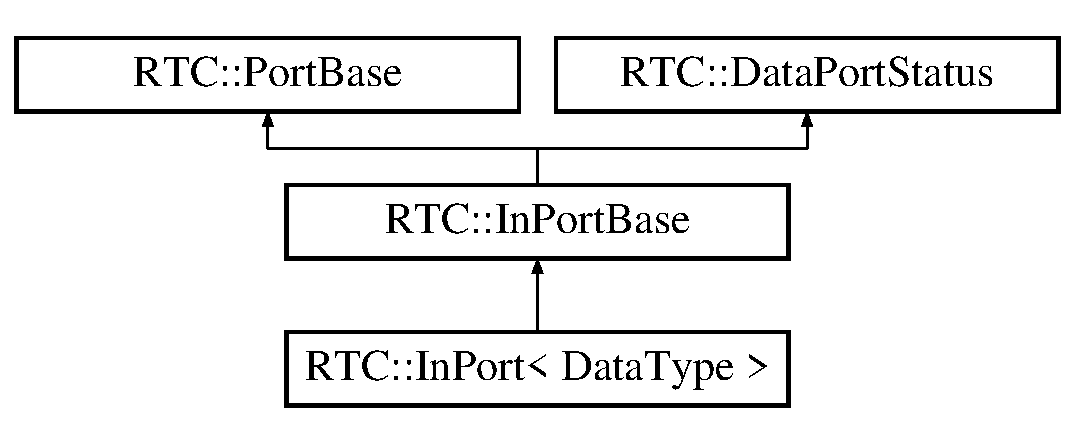
\includegraphics[height=3cm]{classRTC_1_1InPort}
\end{center}
\end{figure}
\subsection*{Public Member Functions}
\begin{DoxyCompactItemize}
\item 
DATAPORTSTATUS\_\-ENUM {\bf InPort} (const char $\ast$name, DataType \&value, int bufsize=64, bool read\_\-block=false, bool write\_\-block=false, int read\_\-timeout=0, int write\_\-timeout=0)
\begin{DoxyCompactList}\small\item\em A constructor. \item\end{DoxyCompactList}\item 
virtual {\bf $\sim$InPort} (void)
\begin{DoxyCompactList}\small\item\em Destructor. \item\end{DoxyCompactList}\item 
virtual const char $\ast$ {\bf name} ()
\begin{DoxyCompactList}\small\item\em Get port name. \item\end{DoxyCompactList}\item 
virtual bool {\bf isNew} ()
\begin{DoxyCompactList}\small\item\em Check whether the data is newest. \item\end{DoxyCompactList}\item 
virtual bool {\bf isEmpty} ()
\begin{DoxyCompactList}\small\item\em Check whether the data is newest. \item\end{DoxyCompactList}\item 
bool {\bf read} ()
\begin{DoxyCompactList}\small\item\em Readout the value from DataPort. \item\end{DoxyCompactList}\item 
virtual void {\bf update} ()
\begin{DoxyCompactList}\small\item\em Read the newly value to type-\/T variable which is bound to InPort's buffer. \item\end{DoxyCompactList}\item 
void {\bf operator$>$$>$} (DataType \&rhs)
\begin{DoxyCompactList}\small\item\em Read the newly value data in \doxyref{InPort}{p.}{classRTC_1_1InPort} to type-\/T variable. \item\end{DoxyCompactList}\item 
void {\bf setOnRead} ({\bf OnRead}$<$ DataType $>$ $\ast$on\_\-read)
\begin{DoxyCompactList}\small\item\em Set callback when data is read from the \doxyref{InPort}{p.}{classRTC_1_1InPort} buffer. \item\end{DoxyCompactList}\item 
void {\bf setOnReadConvert} ({\bf OnReadConvert}$<$ DataType $>$ $\ast$on\_\-rconvert)
\begin{DoxyCompactList}\small\item\em Set callback when data is readout to the \doxyref{InPort}{p.}{classRTC_1_1InPort} buffer. \item\end{DoxyCompactList}\end{DoxyCompactItemize}


\subsection{Detailed Description}
\subsubsection*{template$<$class DataType$>$ class RTC::InPort$<$ DataType $>$}

\doxyref{InPort}{p.}{classRTC_1_1InPort} template class. This is a template class that implements \doxyref{InPort}{p.}{classRTC_1_1InPort}. $<$T$>$ is the type defined in BasicDataType.idl and must be the structure which has both Time type tm and type-\/T data as a member. \doxyref{InPort}{p.}{classRTC_1_1InPort} has a ring buffer internally, and stores the received data externally in this buffer one by one. The size of ring buffer can be specified according to the argument of constructor, though the default size is 64. Unread data and data which is already read are managed with the flag, and the data can be handled by the \doxyref{isNew()}{p.}{classRTC_1_1InPort_af3030dcf08e4951924407df3e71fc123}, write(), \doxyref{read()}{p.}{classRTC_1_1InPort_a1b6e58e0c821b46148266ddfd0b9bd54}, isFull() and \doxyref{isEmpty()}{p.}{classRTC_1_1InPort_a0bf0a0b180a60961fa7559aa54af57ca} method etc.

\begin{DoxySince}{Since}
0.2.0 
\end{DoxySince}


\subsection{Constructor \& Destructor Documentation}
\index{RTC::InPort@{RTC::InPort}!InPort@{InPort}}
\index{InPort@{InPort}!RTC::InPort@{RTC::InPort}}
\subsubsection[{InPort}]{\setlength{\rightskip}{0pt plus 5cm}template$<$class DataType $>$ DATAPORTSTATUS\_\-ENUM {\bf RTC::InPort}$<$ DataType $>$::{\bf InPort} (const char $\ast$ {\em name}, \/  DataType \& {\em value}, \/  int {\em bufsize} = {\ttfamily 64}, \/  bool {\em read\_\-block} = {\ttfamily false}, \/  bool {\em write\_\-block} = {\ttfamily false}, \/  int {\em read\_\-timeout} = {\ttfamily 0}, \/  int {\em write\_\-timeout} = {\ttfamily 0})\hspace{0.3cm}{\ttfamily  [inline]}}\label{classRTC_1_1InPort_a8450177baa07f202144fbba039f4b827}


A constructor. 

constructor. This is bound to type-\/T variable given as a parameter.


\begin{DoxyParams}{Parameters}
\item[{\em name}]A name of the \doxyref{InPort}{p.}{classRTC_1_1InPort}. This name is referred by InPortBase::name(). \item[{\em value}]type-\/T variable that is bound to this \doxyref{InPort}{p.}{classRTC_1_1InPort}. \item[{\em bufsize}]Buffer length of internal ring buffer of \doxyref{InPort}{p.}{classRTC_1_1InPort} (The default value:64) \item[{\em read\_\-block}]Flag of reading block. When there are not unread data at reading data, set whether to block data until receiving the next data. (The default value:false) \item[{\em write\_\-block}]Flag of writing block. If the buffer was full at writing data, set whether to block data until the buffer has space. (The default value:false) \item[{\em read\_\-timeout}]Data reading timeout time (millisecond) when not specifying read blocking. (The default value:0) \item[{\em write\_\-timeout}]Data writing timeout time (millisecond) when not specifying writing block. (The default value:0) \end{DoxyParams}
\index{RTC::InPort@{RTC::InPort}!$\sim$InPort@{$\sim$InPort}}
\index{$\sim$InPort@{$\sim$InPort}!RTC::InPort@{RTC::InPort}}
\subsubsection[{$\sim$InPort}]{\setlength{\rightskip}{0pt plus 5cm}template$<$class DataType $>$ virtual {\bf RTC::InPort}$<$ DataType $>$::$\sim${\bf InPort} (void)\hspace{0.3cm}{\ttfamily  [inline, virtual]}}\label{classRTC_1_1InPort_a42532e8164d15bbb92cdce9ff5f3baf8}


Destructor. 

Destructor 

\subsection{Member Function Documentation}
\index{RTC::InPort@{RTC::InPort}!isEmpty@{isEmpty}}
\index{isEmpty@{isEmpty}!RTC::InPort@{RTC::InPort}}
\subsubsection[{isEmpty}]{\setlength{\rightskip}{0pt plus 5cm}template$<$class DataType $>$ virtual bool {\bf RTC::InPort}$<$ DataType $>$::isEmpty (void)\hspace{0.3cm}{\ttfamily  [inline, virtual]}}\label{classRTC_1_1InPort_a0bf0a0b180a60961fa7559aa54af57ca}


Check whether the data is newest. 

Check whether the data stored at a current buffer position is newest.

\begin{DoxyReturn}{Returns}
Newest data check result ( true:Newest data. Data has not been readout yet. false:Past data.Data has already been readout.) 
\end{DoxyReturn}


References RTC::InPortBase::m\_\-connectors, RTC::PortBase::m\_\-connectorsMutex, RTC\_\-DEBUG, and RTC\_\-TRACE.

\index{RTC::InPort@{RTC::InPort}!isNew@{isNew}}
\index{isNew@{isNew}!RTC::InPort@{RTC::InPort}}
\subsubsection[{isNew}]{\setlength{\rightskip}{0pt plus 5cm}template$<$class DataType $>$ virtual bool {\bf RTC::InPort}$<$ DataType $>$::isNew ()\hspace{0.3cm}{\ttfamily  [inline, virtual]}}\label{classRTC_1_1InPort_af3030dcf08e4951924407df3e71fc123}


Check whether the data is newest. 

Check whether the data stored at a current buffer position is newest.

\begin{DoxyReturn}{Returns}
Newest data check result ( true:Newest data. Data has not been readout yet. false:Past data.Data has already been readout.) 
\end{DoxyReturn}


References RTC::InPortBase::m\_\-connectors, RTC::PortBase::m\_\-connectorsMutex, RTC\_\-DEBUG, and RTC\_\-TRACE.

\index{RTC::InPort@{RTC::InPort}!name@{name}}
\index{name@{name}!RTC::InPort@{RTC::InPort}}
\subsubsection[{name}]{\setlength{\rightskip}{0pt plus 5cm}template$<$class DataType $>$ virtual const char$\ast$ {\bf RTC::InPort}$<$ DataType $>$::name ()\hspace{0.3cm}{\ttfamily  [inline, virtual]}}\label{classRTC_1_1InPort_ae8e026ff3e775a211022e2a108d8a672}


Get port name. 

Get port name.

\begin{DoxyReturn}{Returns}
The port name 
\end{DoxyReturn}
\index{RTC::InPort@{RTC::InPort}!operator$>$$>$@{operator$>$$>$}}
\index{operator$>$$>$@{operator$>$$>$}!RTC::InPort@{RTC::InPort}}
\subsubsection[{operator$>$$>$}]{\setlength{\rightskip}{0pt plus 5cm}template$<$class DataType $>$ void {\bf RTC::InPort}$<$ DataType $>$::operator$>$$>$ (DataType \& {\em rhs})\hspace{0.3cm}{\ttfamily  [inline]}}\label{classRTC_1_1InPort_a44cc1bb1cf583f7b88578e39c04b5ea5}


Read the newly value data in \doxyref{InPort}{p.}{classRTC_1_1InPort} to type-\/T variable. 

Read the newly data set in \doxyref{InPort}{p.}{classRTC_1_1InPort} and set to specified data variable.


\begin{DoxyParams}{Parameters}
\item[{\em rhs}]The type-\/T variable to read from InPort's buffer \end{DoxyParams}


References RTC::InPort$<$ DataType $>$::read().

\index{RTC::InPort@{RTC::InPort}!read@{read}}
\index{read@{read}!RTC::InPort@{RTC::InPort}}
\subsubsection[{read}]{\setlength{\rightskip}{0pt plus 5cm}template$<$class DataType $>$ bool {\bf RTC::InPort}$<$ DataType $>$::read ()\hspace{0.3cm}{\ttfamily  [inline, virtual]}}\label{classRTC_1_1InPort_a1b6e58e0c821b46148266ddfd0b9bd54}


Readout the value from DataPort. 

Readout the value from DataPort


\begin{DoxyItemize}
\item When Callback functor \doxyref{OnRead}{p.}{structRTC_1_1OnRead} is already set, \doxyref{OnRead}{p.}{structRTC_1_1OnRead} will be invoked before reading from the buffer held by DataPort.
\item When the buffer held by DataPort can detect the underflow, and when it detected the underflow at reading, callback functor OnUnderflow will be invoked.
\item When callback functor \doxyref{OnReadConvert}{p.}{structRTC_1_1OnReadConvert} is already set, the return value of operator() of \doxyref{OnReadConvert}{p.}{structRTC_1_1OnReadConvert} will be the return value of \doxyref{read()}{p.}{classRTC_1_1InPort_a1b6e58e0c821b46148266ddfd0b9bd54}.
\item When timeout of reading is already set by setReadTimeout(), it waits for only timeout time until the state of the buffer underflow is reset, and if OnUnderflow is already set, this will be invoked to return.
\end{DoxyItemize}

\begin{DoxyReturn}{Returns}
Readout result (Successful:true, Failed:false) 
\end{DoxyReturn}


Implements {\bf RTC::InPortBase} \doxyref{}{p.}{classRTC_1_1InPortBase_a448e72f4d6d7890c4fb6add7d86d04b5}.



References RTC::DataPortStatus::BUFFER\_\-EMPTY, RTC::DataPortStatus::BUFFER\_\-TIMEOUT, RTC::InPortBase::m\_\-connectors, RTC::PortBase::m\_\-connectorsMutex, RTC::DataPortStatus::PORT\_\-OK, RTC\_\-DEBUG, RTC\_\-ERROR, RTC\_\-TRACE, and RTC\_\-WARN.



Referenced by RTC::InPort$<$ DataType $>$::operator$>$$>$(), and RTC::InPort$<$ DataType $>$::update().

\index{RTC::InPort@{RTC::InPort}!setOnRead@{setOnRead}}
\index{setOnRead@{setOnRead}!RTC::InPort@{RTC::InPort}}
\subsubsection[{setOnRead}]{\setlength{\rightskip}{0pt plus 5cm}template$<$class DataType $>$ void {\bf RTC::InPort}$<$ DataType $>$::setOnRead ({\bf OnRead}$<$ DataType $>$ $\ast$ {\em on\_\-read})\hspace{0.3cm}{\ttfamily  [inline]}}\label{classRTC_1_1InPort_a93fe41858e1e8dd7dee71b64703b7343}


Set callback when data is read from the \doxyref{InPort}{p.}{classRTC_1_1InPort} buffer. 

Set the callback object that is invoked right before data is read from the InPort's buffer


\begin{DoxyParams}{Parameters}
\item[{\em on\_\-read}]\doxyref{OnRead}{p.}{structRTC_1_1OnRead}$<$DataType$>$ type object \end{DoxyParams}
\index{RTC::InPort@{RTC::InPort}!setOnReadConvert@{setOnReadConvert}}
\index{setOnReadConvert@{setOnReadConvert}!RTC::InPort@{RTC::InPort}}
\subsubsection[{setOnReadConvert}]{\setlength{\rightskip}{0pt plus 5cm}template$<$class DataType $>$ void {\bf RTC::InPort}$<$ DataType $>$::setOnReadConvert ({\bf OnReadConvert}$<$ DataType $>$ $\ast$ {\em on\_\-rconvert})\hspace{0.3cm}{\ttfamily  [inline]}}\label{classRTC_1_1InPort_af799d52ed11a670ef56da9a2b2a9e7ff}


Set callback when data is readout to the \doxyref{InPort}{p.}{classRTC_1_1InPort} buffer. 

Set the callback object that is invoked when data is readout to the InPort's buffer. The return value of callback object is the return result of the \doxyref{read()}{p.}{classRTC_1_1InPort_a1b6e58e0c821b46148266ddfd0b9bd54} method.


\begin{DoxyParams}{Parameters}
\item[{\em on\_\-rconvert}]\doxyref{OnReadConvert}{p.}{structRTC_1_1OnReadConvert}$<$DataType$>$ type object \end{DoxyParams}
\index{RTC::InPort@{RTC::InPort}!update@{update}}
\index{update@{update}!RTC::InPort@{RTC::InPort}}
\subsubsection[{update}]{\setlength{\rightskip}{0pt plus 5cm}template$<$class DataType $>$ virtual void {\bf RTC::InPort}$<$ DataType $>$::update (void)\hspace{0.3cm}{\ttfamily  [inline, virtual]}}\label{classRTC_1_1InPort_ad1efc0019d9a62030106552ad4f4436d}


Read the newly value to type-\/T variable which is bound to InPort's buffer. 

Read the newly value to type-\/T data which is bound to InPort's buffer. The type-\/T variable must be bound to \doxyref{InPort}{p.}{classRTC_1_1InPort} in constructor. Since this method assumes to be used for polymorphic, its argument and the return value do not depend on type. 

References RTC::InPort$<$ DataType $>$::read().


\section{RTC::InPortBase Class Reference}
\label{classRTC_1_1InPortBase}\index{RTC::InPortBase@{RTC::InPortBase}}


Port for \doxyref{InPort}{p.}{classRTC_1_1InPort}.  




{\ttfamily \#include $<$InPortBase.h$>$}

Inheritance diagram for RTC::InPortBase:\begin{figure}[H]
\begin{center}
\leavevmode
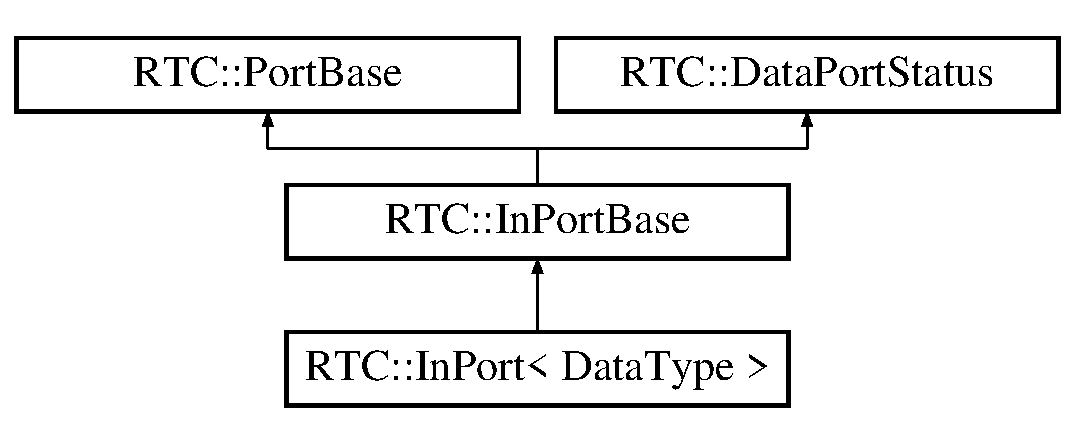
\includegraphics[height=3cm]{classRTC_1_1InPortBase}
\end{center}
\end{figure}
\subsection*{Public Member Functions}
\begin{DoxyCompactItemize}
\item 
{\bf InPortBase} (const char $\ast$name, const char $\ast$data\_\-type)
\begin{DoxyCompactList}\small\item\em Constructor. \item\end{DoxyCompactList}\item 
virtual {\bf $\sim$InPortBase} (void)
\begin{DoxyCompactList}\small\item\em Destructor. \item\end{DoxyCompactList}\item 
void {\bf init} ({\bf coil::Properties} \&prop)
\begin{DoxyCompactList}\small\item\em Initializing properties. \item\end{DoxyCompactList}\item 
virtual bool {\bf read} ()=0
\begin{DoxyCompactList}\small\item\em It is a virtual method that is called from \doxyref{RTObject\_\-impl::readAll()}{p.}{classRTC_1_1RTObject__impl_a69b50eea5bc7f862114602963cca84ca}. This method reads out data from DataPort. \item\end{DoxyCompactList}\item 
{\bf coil::Properties} \& {\bf properties} ()
\begin{DoxyCompactList}\small\item\em Get properties. \item\end{DoxyCompactList}\item 
const std::vector$<$ {\bf InPortConnector} $\ast$ $>$ \& {\bf connectors} ()
\begin{DoxyCompactList}\small\item\em Connector list. \item\end{DoxyCompactList}\item 
{\bf ConnectorInfoList} {\bf getConnectorProfiles} ()
\begin{DoxyCompactList}\small\item\em ConnectorProfile list. \item\end{DoxyCompactList}\item 
{\bf coil::vstring} {\bf getConnectorIds} ()
\begin{DoxyCompactList}\small\item\em ConnectorId list. \item\end{DoxyCompactList}\item 
{\bf coil::vstring} {\bf getConnectorNames} ()
\begin{DoxyCompactList}\small\item\em Connector name list. \item\end{DoxyCompactList}\item 
{\bf InPortConnector} $\ast$ {\bf getConnectorById} (const char $\ast$id)
\begin{DoxyCompactList}\small\item\em Getting ConnectorProfile by ID. \item\end{DoxyCompactList}\item 
{\bf InPortConnector} $\ast$ {\bf getConnectorByName} (const char $\ast$name)
\begin{DoxyCompactList}\small\item\em Getting Connector by name. \item\end{DoxyCompactList}\item 
bool {\bf getConnectorProfileById} (const char $\ast$id, {\bf ConnectorInfo} \&prof)
\begin{DoxyCompactList}\small\item\em Getting ConnectorProfile by name. \item\end{DoxyCompactList}\item 
bool {\bf getConnectorProfileByName} (const char $\ast$name, {\bf ConnectorInfo} \&prof)
\begin{DoxyCompactList}\small\item\em Getting ConnectorProfile by name. \item\end{DoxyCompactList}\item 
virtual void {\bf activateInterfaces} ()
\begin{DoxyCompactList}\small\item\em Activate all Port interfaces. \item\end{DoxyCompactList}\item 
virtual void {\bf deactivateInterfaces} ()
\begin{DoxyCompactList}\small\item\em Deactivate all Port interfaces. \item\end{DoxyCompactList}\item 
void {\bf addConnectorDataListener} ({\bf ConnectorDataListenerType} listener\_\-type, {\bf ConnectorDataListener} $\ast$listener, bool autoclean=true)
\begin{DoxyCompactList}\small\item\em Adding BufferDataListener type listener. \item\end{DoxyCompactList}\item 
void {\bf removeConnectorDataListener} ({\bf ConnectorDataListenerType} listener\_\-type, {\bf ConnectorDataListener} $\ast$listener)
\begin{DoxyCompactList}\small\item\em Removing BufferDataListener type listener. \item\end{DoxyCompactList}\item 
void {\bf addConnectorListener} ({\bf ConnectorListenerType} callback\_\-type, {\bf ConnectorListener} $\ast$listener, bool autoclean=true)
\begin{DoxyCompactList}\small\item\em Adding \doxyref{ConnectorListener}{p.}{classRTC_1_1ConnectorListener} type listener. \item\end{DoxyCompactList}\item 
void {\bf removeConnectorListener} ({\bf ConnectorListenerType} callback\_\-type, {\bf ConnectorListener} $\ast$listener)
\begin{DoxyCompactList}\small\item\em Removing BufferDataListener type listener. \item\end{DoxyCompactList}\item 
bool {\bf isLittleEndian} ()
\begin{DoxyCompactList}\small\item\em return it whether endian setting. \item\end{DoxyCompactList}\item 
virtual ReturnCode\_\-t {\bf connect} (ConnectorProfile \&connector\_\-profile)  throw (CORBA::SystemException)
\begin{DoxyCompactList}\small\item\em [CORBA interface] Connect the Port \item\end{DoxyCompactList}\end{DoxyCompactItemize}
\subsection*{Public Attributes}
\begin{DoxyCompactItemize}
\item 
DATAPORTSTATUS\_\-ENUM typedef std::vector$<$ {\bf InPortConnector} $\ast$ $>$ {\bf ConnectorList}
\end{DoxyCompactItemize}
\subsection*{Protected Member Functions}
\begin{DoxyCompactItemize}
\item 
virtual ReturnCode\_\-t {\bf publishInterfaces} (ConnectorProfile \&connector\_\-profile)
\begin{DoxyCompactList}\small\item\em Publish interface information. \item\end{DoxyCompactList}\item 
virtual ReturnCode\_\-t {\bf subscribeInterfaces} (const ConnectorProfile \&connector\_\-profile)
\begin{DoxyCompactList}\small\item\em Subscribe to the interface. \item\end{DoxyCompactList}\item 
virtual void {\bf unsubscribeInterfaces} (const ConnectorProfile \&connector\_\-profile)
\begin{DoxyCompactList}\small\item\em Disconnect the interface connection. \item\end{DoxyCompactList}\item 
void {\bf initProviders} ()
\begin{DoxyCompactList}\small\item\em \doxyref{InPort}{p.}{classRTC_1_1InPort} provider initialization. \item\end{DoxyCompactList}\item 
void {\bf initConsumers} ()
\begin{DoxyCompactList}\small\item\em \doxyref{OutPort}{p.}{classRTC_1_1OutPort} consumer initialization. \item\end{DoxyCompactList}\item 
bool {\bf checkEndian} (const {\bf coil::Properties} \&prop, bool \&littleEndian)
\begin{DoxyCompactList}\small\item\em Checking endian flag of serializer. \item\end{DoxyCompactList}\item 
{\bf InPortProvider} $\ast$ {\bf createProvider} (ConnectorProfile \&cprof, {\bf coil::Properties} \&prop)
\begin{DoxyCompactList}\small\item\em \doxyref{InPort}{p.}{classRTC_1_1InPort} provider creation. \item\end{DoxyCompactList}\item 
{\bf OutPortConsumer} $\ast$ {\bf createConsumer} (const ConnectorProfile \&cprof, {\bf coil::Properties} \&prop)
\begin{DoxyCompactList}\small\item\em \doxyref{InPort}{p.}{classRTC_1_1InPort} provider creation. \item\end{DoxyCompactList}\item 
{\bf InPortConnector} $\ast$ {\bf createConnector} (ConnectorProfile \&cprof, {\bf coil::Properties} \&prop, {\bf InPortProvider} $\ast$provider)
\begin{DoxyCompactList}\small\item\em \doxyref{InPortPushConnector}{p.}{classRTC_1_1InPortPushConnector} creation. \item\end{DoxyCompactList}\item 
{\bf InPortConnector} $\ast$ {\bf createConnector} (const ConnectorProfile \&cprof, {\bf coil::Properties} \&prop, {\bf OutPortConsumer} $\ast$consumer)
\begin{DoxyCompactList}\small\item\em \doxyref{InPortPullConnector}{p.}{classRTC_1_1InPortPullConnector} creation. \item\end{DoxyCompactList}\end{DoxyCompactItemize}
\subsection*{Protected Attributes}
\begin{DoxyCompactItemize}
\item 
bool {\bf m\_\-singlebuffer}
\begin{DoxyCompactList}\small\item\em Buffer mode. \item\end{DoxyCompactList}\item 
{\bf CdrBufferBase} $\ast$ {\bf m\_\-thebuffer}
\begin{DoxyCompactList}\small\item\em Buffer. \item\end{DoxyCompactList}\item 
{\bf coil::Properties} {\bf m\_\-properties}
\begin{DoxyCompactList}\small\item\em Properties. \item\end{DoxyCompactList}\item 
{\bf coil::vstring} {\bf m\_\-providerTypes}
\begin{DoxyCompactList}\small\item\em Available providers. \item\end{DoxyCompactList}\item 
{\bf coil::vstring} {\bf m\_\-consumerTypes}
\begin{DoxyCompactList}\small\item\em Available consumers. \item\end{DoxyCompactList}\item 
{\bf ConnectorList} {\bf m\_\-connectors}
\begin{DoxyCompactList}\small\item\em Connection list. \item\end{DoxyCompactList}\item 
bool {\bf m\_\-littleEndian}
\begin{DoxyCompactList}\small\item\em Connected Endian. \item\end{DoxyCompactList}\item 
{\bf ConnectorListeners} {\bf m\_\-listeners}
\begin{DoxyCompactList}\small\item\em \doxyref{ConnectorDataListener}{p.}{classRTC_1_1ConnectorDataListener} listener. \item\end{DoxyCompactList}\end{DoxyCompactItemize}


\subsection{Detailed Description}
Port for \doxyref{InPort}{p.}{classRTC_1_1InPort}. This is an implementation class for the data input port.

\begin{DoxySince}{Since}
0.4.0 
\end{DoxySince}


\subsection{Constructor \& Destructor Documentation}
\index{RTC::InPortBase@{RTC::InPortBase}!InPortBase@{InPortBase}}
\index{InPortBase@{InPortBase}!RTC::InPortBase@{RTC::InPortBase}}
\subsubsection[{InPortBase}]{\setlength{\rightskip}{0pt plus 5cm}RTC::InPortBase::InPortBase (const char $\ast$ {\em name}, \/  const char $\ast$ {\em data\_\-type})}\label{classRTC_1_1InPortBase_acf7e8f976e2d5c40132a02fe309b1f1e}


Constructor. 

Constructor


\begin{DoxyParams}{Parameters}
\item[{\em name}]Port name \item[{\em data\_\-type}]Data type \end{DoxyParams}
\index{RTC::InPortBase@{RTC::InPortBase}!$\sim$InPortBase@{$\sim$InPortBase}}
\index{$\sim$InPortBase@{$\sim$InPortBase}!RTC::InPortBase@{RTC::InPortBase}}
\subsubsection[{$\sim$InPortBase}]{\setlength{\rightskip}{0pt plus 5cm}virtual RTC::InPortBase::$\sim$InPortBase (void)\hspace{0.3cm}{\ttfamily  [virtual]}}\label{classRTC_1_1InPortBase_a32e533d6c608f0d6125440b7366c857c}


Destructor. 

Destructor 

\subsection{Member Function Documentation}
\index{RTC::InPortBase@{RTC::InPortBase}!activateInterfaces@{activateInterfaces}}
\index{activateInterfaces@{activateInterfaces}!RTC::InPortBase@{RTC::InPortBase}}
\subsubsection[{activateInterfaces}]{\setlength{\rightskip}{0pt plus 5cm}virtual void RTC::InPortBase::activateInterfaces ()\hspace{0.3cm}{\ttfamily  [virtual]}}\label{classRTC_1_1InPortBase_a4188e629df750498e0d3b100f51133ff}


Activate all Port interfaces. 

This operation activate all interfaces that is registered in the ports. 

Implements {\bf RTC::PortBase} \doxyref{}{p.}{classRTC_1_1PortBase_ad779347bae007555968dda9e78004e34}.

\index{RTC::InPortBase@{RTC::InPortBase}!addConnectorDataListener@{addConnectorDataListener}}
\index{addConnectorDataListener@{addConnectorDataListener}!RTC::InPortBase@{RTC::InPortBase}}
\subsubsection[{addConnectorDataListener}]{\setlength{\rightskip}{0pt plus 5cm}void RTC::InPortBase::addConnectorDataListener ({\bf ConnectorDataListenerType} {\em listener\_\-type}, \/  {\bf ConnectorDataListener} $\ast$ {\em listener}, \/  bool {\em autoclean} = {\ttfamily true})}\label{classRTC_1_1InPortBase_a87108f42506a526d05dd72d67a1654af}


Adding BufferDataListener type listener. 

This operation adds certain listeners related to buffer writing and reading events. The following listener types are available.


\begin{DoxyItemize}
\item ON\_\-BUFFER\_\-WRITE: At the time of buffer write
\item ON\_\-BUFFER\_\-FULL: At the time of buffer full
\item ON\_\-BUFFER\_\-WRITE\_\-TIMEOUT: At the time of buffer write timeout
\item ON\_\-BUFFER\_\-OVERWRITE: At the time of buffer overwrite
\item ON\_\-BUFFER\_\-READ: At the time of buffer read
\item ON\_\-SEND: At the time of sending to \doxyref{InPort}{p.}{classRTC_1_1InPort}
\item ON\_\-RECEIVED: At the time of finishing sending to \doxyref{InPort}{p.}{classRTC_1_1InPort}
\item ON\_\-SENDER\_\-TIMEOUT: At the time of timeout of \doxyref{OutPort}{p.}{classRTC_1_1OutPort}
\item ON\_\-SENDER\_\-ERROR: At the time of error of \doxyref{OutPort}{p.}{classRTC_1_1OutPort}
\item ON\_\-RECEIVER\_\-FULL: At the time of bufferfull of \doxyref{InPort}{p.}{classRTC_1_1InPort}
\item ON\_\-RECEIVER\_\-TIMEOUT: At the time of timeout of \doxyref{InPort}{p.}{classRTC_1_1InPort}
\item ON\_\-RECEIVER\_\-ERROR: At the time of error of \doxyref{InPort}{p.}{classRTC_1_1InPort}
\end{DoxyItemize}

Listeners should have the following function operator().

\doxyref{ConnectorDataListener}{p.}{classRTC_1_1ConnectorDataListener}:: operator()(const ConnectorProfile\&, const cdrStream\&)

The ownership of the given listener object is transferred to this \doxyref{OutPort}{p.}{classRTC_1_1OutPort} object in default. The given listener object will be destroied automatically in the OutPort's dtor or if the listener is deleted by \doxyref{removeConnectorDataListener()}{p.}{classRTC_1_1InPortBase_ad371ba04fc81e381ff74751bc2f400c9} function. If you want to keep ownership of the listener object, give \char`\"{}false\char`\"{} value to 3rd argument to inhibit automatic destruction.


\begin{DoxyParams}{Parameters}
\item[{\em listener\_\-type}]A listener type \item[{\em listener}]A pointer to a listener object \item[{\em autoclean}]A flag for automatic listener destruction \end{DoxyParams}
\index{RTC::InPortBase@{RTC::InPortBase}!addConnectorListener@{addConnectorListener}}
\index{addConnectorListener@{addConnectorListener}!RTC::InPortBase@{RTC::InPortBase}}
\subsubsection[{addConnectorListener}]{\setlength{\rightskip}{0pt plus 5cm}void RTC::InPortBase::addConnectorListener ({\bf ConnectorListenerType} {\em callback\_\-type}, \/  {\bf ConnectorListener} $\ast$ {\em listener}, \/  bool {\em autoclean} = {\ttfamily true})}\label{classRTC_1_1InPortBase_af3f78ee20e085969a55854b6bcacb0f0}


Adding \doxyref{ConnectorListener}{p.}{classRTC_1_1ConnectorListener} type listener. 

This operation adds certain listeners related to buffer writing and reading events. The following listener types are available.


\begin{DoxyItemize}
\item ON\_\-BUFFER\_\-EMPTY: At the time of buffer empty
\item ON\_\-BUFFER\_\-READTIMEOUT: At the time of buffer read timeout
\end{DoxyItemize}

Listeners should have the following function operator().

ConnectorListener::operator()(const ConnectorProfile\&)

The ownership of the given listener object is transferred to this \doxyref{OutPort}{p.}{classRTC_1_1OutPort} object in default. The given listener object will be destroied automatically in the OutPort's dtor or if the listener is deleted by \doxyref{removeConnectorListener()}{p.}{classRTC_1_1InPortBase_a28f441f50e37fd06c7cf7c4c5b02e321} function. If you want to keep ownership of the listener object, give \char`\"{}false\char`\"{} value to 3rd argument to inhibit automatic destruction.


\begin{DoxyParams}{Parameters}
\item[{\em listener\_\-type}]A listener type \item[{\em listener}]A pointer to a listener object \item[{\em autoclean}]A flag for automatic listener destruction \end{DoxyParams}
\index{RTC::InPortBase@{RTC::InPortBase}!checkEndian@{checkEndian}}
\index{checkEndian@{checkEndian}!RTC::InPortBase@{RTC::InPortBase}}
\subsubsection[{checkEndian}]{\setlength{\rightskip}{0pt plus 5cm}bool RTC::InPortBase::checkEndian (const {\bf coil::Properties} \& {\em prop}, \/  bool \& {\em littleEndian})\hspace{0.3cm}{\ttfamily  [protected]}}\label{classRTC_1_1InPortBase_ae32b6fb379655aeaf86db44db06e6d77}


Checking endian flag of serializer. 

This operation checks endian flag of data serializer that is specified properties. If valid specification is found, this operation returns true and set argument littleEndian. True means little endian, false means big endian.


\begin{DoxyParams}{Parameters}
\item[{\em prop}]Properties \item[{\em littleEndian}]Endian Information(true:little,false:big) \end{DoxyParams}
\begin{DoxyReturn}{Returns}
true:\char`\"{}Serializer\char`\"{} key doesn't exist. or \char`\"{}Serializer\char`\"{} key exists and there is a content.
\end{DoxyReturn}
false:There is no content though \char`\"{}Serializer\char`\"{} key exists. or ithe content is not \char`\"{}Little. \char`\"{} though \char`\"{}Serializer\char`\"{} key exists. or The content is not \char`\"{}little\char`\"{} or \char`\"{}big\char`\"{} though \char`\"{}Serializer\char`\"{} key exists. \index{RTC::InPortBase@{RTC::InPortBase}!connect@{connect}}
\index{connect@{connect}!RTC::InPortBase@{RTC::InPortBase}}
\subsubsection[{connect}]{\setlength{\rightskip}{0pt plus 5cm}virtual ReturnCode\_\-t RTC::InPortBase::connect (ConnectorProfile \& {\em connector\_\-profile})  throw (CORBA::SystemException)\hspace{0.3cm}{\ttfamily  [virtual]}}\label{classRTC_1_1InPortBase_ab37ad76d4270c20133b52b1bbdf3b529}


[CORBA interface] Connect the Port 

This operation establishes connection according to the given ConnectionProfile inforamtion. This function is premised on calling from mainly application program or tools.


\begin{DoxyParams}{Parameters}
\item[{\em connector\_\-profile}]The ConnectorProfile. \end{DoxyParams}
\begin{DoxyReturn}{Returns}
ReturnCode\_\-t The return code of ReturnCode\_\-t type. 
\end{DoxyReturn}


Reimplemented from {\bf RTC::PortBase} \doxyref{}{p.}{classRTC_1_1PortBase_a139d07d2e94f7e793aedf4aa24b92462}.

\index{RTC::InPortBase@{RTC::InPortBase}!connectors@{connectors}}
\index{connectors@{connectors}!RTC::InPortBase@{RTC::InPortBase}}
\subsubsection[{connectors}]{\setlength{\rightskip}{0pt plus 5cm}const std::vector$<${\bf InPortConnector}$\ast$$>$\& RTC::InPortBase::connectors ()}\label{classRTC_1_1InPortBase_a5e247ce406f48bd4cd40ce25d98764d4}


Connector list. 

This operation returns connector list

\begin{DoxyReturn}{Returns}
connector list 
\end{DoxyReturn}
\index{RTC::InPortBase@{RTC::InPortBase}!createConnector@{createConnector}}
\index{createConnector@{createConnector}!RTC::InPortBase@{RTC::InPortBase}}
\subsubsection[{createConnector}]{\setlength{\rightskip}{0pt plus 5cm}{\bf InPortConnector}$\ast$ RTC::InPortBase::createConnector (const ConnectorProfile \& {\em cprof}, \/  {\bf coil::Properties} \& {\em prop}, \/  {\bf OutPortConsumer} $\ast$ {\em consumer})\hspace{0.3cm}{\ttfamily  [protected]}}\label{classRTC_1_1InPortBase_ac7be351658bb18c655b7fea9a2dac68b}


\doxyref{InPortPullConnector}{p.}{classRTC_1_1InPortPullConnector} creation. 

\index{RTC::InPortBase@{RTC::InPortBase}!createConnector@{createConnector}}
\index{createConnector@{createConnector}!RTC::InPortBase@{RTC::InPortBase}}
\subsubsection[{createConnector}]{\setlength{\rightskip}{0pt plus 5cm}{\bf InPortConnector}$\ast$ RTC::InPortBase::createConnector (ConnectorProfile \& {\em cprof}, \/  {\bf coil::Properties} \& {\em prop}, \/  {\bf InPortProvider} $\ast$ {\em provider})\hspace{0.3cm}{\ttfamily  [protected]}}\label{classRTC_1_1InPortBase_aa6fe75ede17566f7847394f56700ba6d}


\doxyref{InPortPushConnector}{p.}{classRTC_1_1InPortPushConnector} creation. 

\index{RTC::InPortBase@{RTC::InPortBase}!createConsumer@{createConsumer}}
\index{createConsumer@{createConsumer}!RTC::InPortBase@{RTC::InPortBase}}
\subsubsection[{createConsumer}]{\setlength{\rightskip}{0pt plus 5cm}{\bf OutPortConsumer}$\ast$ RTC::InPortBase::createConsumer (const ConnectorProfile \& {\em cprof}, \/  {\bf coil::Properties} \& {\em prop})\hspace{0.3cm}{\ttfamily  [protected]}}\label{classRTC_1_1InPortBase_a48146d910456ba7b1ebca68e96f77db4}


\doxyref{InPort}{p.}{classRTC_1_1InPort} provider creation. 

\index{RTC::InPortBase@{RTC::InPortBase}!createProvider@{createProvider}}
\index{createProvider@{createProvider}!RTC::InPortBase@{RTC::InPortBase}}
\subsubsection[{createProvider}]{\setlength{\rightskip}{0pt plus 5cm}{\bf InPortProvider}$\ast$ RTC::InPortBase::createProvider (ConnectorProfile \& {\em cprof}, \/  {\bf coil::Properties} \& {\em prop})\hspace{0.3cm}{\ttfamily  [protected]}}\label{classRTC_1_1InPortBase_a4f82e38b34bd3fd392d53f1543da3b58}


\doxyref{InPort}{p.}{classRTC_1_1InPort} provider creation. 

\index{RTC::InPortBase@{RTC::InPortBase}!deactivateInterfaces@{deactivateInterfaces}}
\index{deactivateInterfaces@{deactivateInterfaces}!RTC::InPortBase@{RTC::InPortBase}}
\subsubsection[{deactivateInterfaces}]{\setlength{\rightskip}{0pt plus 5cm}virtual void RTC::InPortBase::deactivateInterfaces ()\hspace{0.3cm}{\ttfamily  [virtual]}}\label{classRTC_1_1InPortBase_a4d8bba26fce07c092ebffbab6b1aa881}


Deactivate all Port interfaces. 

This operation deactivate all interfaces that is registered in the ports. 

Implements {\bf RTC::PortBase} \doxyref{}{p.}{classRTC_1_1PortBase_a8dfb8a33b92b9fc9b6c070df2def633f}.

\index{RTC::InPortBase@{RTC::InPortBase}!getConnectorById@{getConnectorById}}
\index{getConnectorById@{getConnectorById}!RTC::InPortBase@{RTC::InPortBase}}
\subsubsection[{getConnectorById}]{\setlength{\rightskip}{0pt plus 5cm}{\bf InPortConnector}$\ast$ RTC::InPortBase::getConnectorById (const char $\ast$ {\em id})}\label{classRTC_1_1InPortBase_aea583e55d4d025245afd712300230f4f}


Getting ConnectorProfile by ID. 

This operation returns Connector specified by ID.


\begin{DoxyParams}{Parameters}
\item[{\em id}]Connector ID \end{DoxyParams}
\begin{DoxyReturn}{Returns}
A pointer to connector 
\end{DoxyReturn}
\index{RTC::InPortBase@{RTC::InPortBase}!getConnectorByName@{getConnectorByName}}
\index{getConnectorByName@{getConnectorByName}!RTC::InPortBase@{RTC::InPortBase}}
\subsubsection[{getConnectorByName}]{\setlength{\rightskip}{0pt plus 5cm}{\bf InPortConnector}$\ast$ RTC::InPortBase::getConnectorByName (const char $\ast$ {\em name})}\label{classRTC_1_1InPortBase_a322f9c5319fd7102202289b394893bf7}


Getting Connector by name. 

This operation returns Connector specified by name.


\begin{DoxyParams}{Parameters}
\item[{\em id}]Connector ID \end{DoxyParams}
\begin{DoxyReturn}{Returns}
A pointer to connector 
\end{DoxyReturn}
\index{RTC::InPortBase@{RTC::InPortBase}!getConnectorIds@{getConnectorIds}}
\index{getConnectorIds@{getConnectorIds}!RTC::InPortBase@{RTC::InPortBase}}
\subsubsection[{getConnectorIds}]{\setlength{\rightskip}{0pt plus 5cm}{\bf coil::vstring} RTC::InPortBase::getConnectorIds ()}\label{classRTC_1_1InPortBase_a93477a719d89b0da08b23f4da5f48fae}


ConnectorId list. 

This operation returns ConnectorId list

\begin{DoxyReturn}{Returns}
connector list 
\end{DoxyReturn}
\index{RTC::InPortBase@{RTC::InPortBase}!getConnectorNames@{getConnectorNames}}
\index{getConnectorNames@{getConnectorNames}!RTC::InPortBase@{RTC::InPortBase}}
\subsubsection[{getConnectorNames}]{\setlength{\rightskip}{0pt plus 5cm}{\bf coil::vstring} RTC::InPortBase::getConnectorNames ()}\label{classRTC_1_1InPortBase_aa722937ee4e9be0d531db5e207bf0853}


Connector name list. 

This operation returns Connector name list

\begin{DoxyReturn}{Returns}
connector name list 
\end{DoxyReturn}
\index{RTC::InPortBase@{RTC::InPortBase}!getConnectorProfileById@{getConnectorProfileById}}
\index{getConnectorProfileById@{getConnectorProfileById}!RTC::InPortBase@{RTC::InPortBase}}
\subsubsection[{getConnectorProfileById}]{\setlength{\rightskip}{0pt plus 5cm}bool RTC::InPortBase::getConnectorProfileById (const char $\ast$ {\em id}, \/  {\bf ConnectorInfo} \& {\em prof})}\label{classRTC_1_1InPortBase_adffe2b716bbf5ce808010c26ff9cb453}


Getting ConnectorProfile by name. 

This operation returns ConnectorProfile specified by name


\begin{DoxyParams}{Parameters}
\item[{\em id}]Connector ID \item[{\em prof}]ConnectorProfile \end{DoxyParams}
\begin{DoxyReturn}{Returns}
false specified ID does not exist 
\end{DoxyReturn}
\index{RTC::InPortBase@{RTC::InPortBase}!getConnectorProfileByName@{getConnectorProfileByName}}
\index{getConnectorProfileByName@{getConnectorProfileByName}!RTC::InPortBase@{RTC::InPortBase}}
\subsubsection[{getConnectorProfileByName}]{\setlength{\rightskip}{0pt plus 5cm}bool RTC::InPortBase::getConnectorProfileByName (const char $\ast$ {\em name}, \/  {\bf ConnectorInfo} \& {\em prof})}\label{classRTC_1_1InPortBase_ae8ba538d6c318a9ddfb9242a72a6c26b}


Getting ConnectorProfile by name. 

This operation returns ConnectorProfile specified by name


\begin{DoxyParams}{Parameters}
\item[{\em id}]Connector ID \item[{\em prof}]ConnectorProfile \end{DoxyParams}
\begin{DoxyReturn}{Returns}
false specified name does not exist 
\end{DoxyReturn}
\index{RTC::InPortBase@{RTC::InPortBase}!getConnectorProfiles@{getConnectorProfiles}}
\index{getConnectorProfiles@{getConnectorProfiles}!RTC::InPortBase@{RTC::InPortBase}}
\subsubsection[{getConnectorProfiles}]{\setlength{\rightskip}{0pt plus 5cm}{\bf ConnectorInfoList} RTC::InPortBase::getConnectorProfiles ()}\label{classRTC_1_1InPortBase_aa79b490a1fae07ca9a0ed5a99267b608}


ConnectorProfile list. 

This operation returns ConnectorProfile list

\begin{DoxyReturn}{Returns}
connector list 
\end{DoxyReturn}
\index{RTC::InPortBase@{RTC::InPortBase}!init@{init}}
\index{init@{init}!RTC::InPortBase@{RTC::InPortBase}}
\subsubsection[{init}]{\setlength{\rightskip}{0pt plus 5cm}void RTC::InPortBase::init ({\bf coil::Properties} \& {\em prop})}\label{classRTC_1_1InPortBase_adeeb77472583af68e16c1b6ac6aee118}


Initializing properties. 

This method initializes the port in the specified property.


\begin{DoxyParams}{Parameters}
\item[{\em prop}]Property for setting ports \end{DoxyParams}
\index{RTC::InPortBase@{RTC::InPortBase}!initConsumers@{initConsumers}}
\index{initConsumers@{initConsumers}!RTC::InPortBase@{RTC::InPortBase}}
\subsubsection[{initConsumers}]{\setlength{\rightskip}{0pt plus 5cm}void RTC::InPortBase::initConsumers ()\hspace{0.3cm}{\ttfamily  [protected]}}\label{classRTC_1_1InPortBase_aea0abf42128b7f945c3f5787ee19581a}


\doxyref{OutPort}{p.}{classRTC_1_1OutPort} consumer initialization. 

\index{RTC::InPortBase@{RTC::InPortBase}!initProviders@{initProviders}}
\index{initProviders@{initProviders}!RTC::InPortBase@{RTC::InPortBase}}
\subsubsection[{initProviders}]{\setlength{\rightskip}{0pt plus 5cm}void RTC::InPortBase::initProviders ()\hspace{0.3cm}{\ttfamily  [protected]}}\label{classRTC_1_1InPortBase_ac3195cece5da04b052b6d60a99f7c0fa}


\doxyref{InPort}{p.}{classRTC_1_1InPort} provider initialization. 

\index{RTC::InPortBase@{RTC::InPortBase}!isLittleEndian@{isLittleEndian}}
\index{isLittleEndian@{isLittleEndian}!RTC::InPortBase@{RTC::InPortBase}}
\subsubsection[{isLittleEndian}]{\setlength{\rightskip}{0pt plus 5cm}bool RTC::InPortBase::isLittleEndian ()}\label{classRTC_1_1InPortBase_afb766071f5b6f5f7d783a02fbe30ab61}


return it whether endian setting. 

\begin{DoxyReturn}{Returns}
Return true in the case of \char`\"{}little\char`\"{}, false in \char`\"{}big\char`\"{} than it. 
\end{DoxyReturn}
\index{RTC::InPortBase@{RTC::InPortBase}!properties@{properties}}
\index{properties@{properties}!RTC::InPortBase@{RTC::InPortBase}}
\subsubsection[{properties}]{\setlength{\rightskip}{0pt plus 5cm}{\bf coil::Properties}\& RTC::InPortBase::properties ()}\label{classRTC_1_1InPortBase_a86cfb64b99b76f6ae34288704fdf4ed4}


Get properties. 

This method gets properties in the port.

\begin{DoxyReturn}{Returns}
Properties 
\end{DoxyReturn}
\index{RTC::InPortBase@{RTC::InPortBase}!publishInterfaces@{publishInterfaces}}
\index{publishInterfaces@{publishInterfaces}!RTC::InPortBase@{RTC::InPortBase}}
\subsubsection[{publishInterfaces}]{\setlength{\rightskip}{0pt plus 5cm}virtual ReturnCode\_\-t RTC::InPortBase::publishInterfaces (ConnectorProfile \& {\em connector\_\-profile})\hspace{0.3cm}{\ttfamily  [protected, virtual]}}\label{classRTC_1_1InPortBase_ad836b599b157efb1a31ec61999015986}


Publish interface information. 

Publish interface information. Assign the Provider information that owned by this port to ConnectorProfile::properties


\begin{DoxyParams}{Parameters}
\item[{\em connector\_\-profile}]The connector profile\end{DoxyParams}
\begin{DoxyReturn}{Returns}
The return code of ReturnCode\_\-t type 
\end{DoxyReturn}


Implements {\bf RTC::PortBase} \doxyref{}{p.}{classRTC_1_1PortBase_acf31878c5912f56c122aaa2310e182de}.

\index{RTC::InPortBase@{RTC::InPortBase}!read@{read}}
\index{read@{read}!RTC::InPortBase@{RTC::InPortBase}}
\subsubsection[{read}]{\setlength{\rightskip}{0pt plus 5cm}virtual bool RTC::InPortBase::read ()\hspace{0.3cm}{\ttfamily  [pure virtual]}}\label{classRTC_1_1InPortBase_a448e72f4d6d7890c4fb6add7d86d04b5}


It is a virtual method that is called from \doxyref{RTObject\_\-impl::readAll()}{p.}{classRTC_1_1RTObject__impl_a69b50eea5bc7f862114602963cca84ca}. This method reads out data from DataPort. 

\begin{DoxyReturn}{Returns}
true:Success,false:Failure 
\end{DoxyReturn}


Implemented in {\bf RTC::InPort$<$ DataType $>$} \doxyref{}{p.}{classRTC_1_1InPort_a1b6e58e0c821b46148266ddfd0b9bd54}.

\index{RTC::InPortBase@{RTC::InPortBase}!removeConnectorDataListener@{removeConnectorDataListener}}
\index{removeConnectorDataListener@{removeConnectorDataListener}!RTC::InPortBase@{RTC::InPortBase}}
\subsubsection[{removeConnectorDataListener}]{\setlength{\rightskip}{0pt plus 5cm}void RTC::InPortBase::removeConnectorDataListener ({\bf ConnectorDataListenerType} {\em listener\_\-type}, \/  {\bf ConnectorDataListener} $\ast$ {\em listener})}\label{classRTC_1_1InPortBase_ad371ba04fc81e381ff74751bc2f400c9}


Removing BufferDataListener type listener. 

This operation removes a specified listener.


\begin{DoxyParams}{Parameters}
\item[{\em listener\_\-type}]A listener type \item[{\em listener}]A pointer to a listener object \end{DoxyParams}
\index{RTC::InPortBase@{RTC::InPortBase}!removeConnectorListener@{removeConnectorListener}}
\index{removeConnectorListener@{removeConnectorListener}!RTC::InPortBase@{RTC::InPortBase}}
\subsubsection[{removeConnectorListener}]{\setlength{\rightskip}{0pt plus 5cm}void RTC::InPortBase::removeConnectorListener ({\bf ConnectorListenerType} {\em callback\_\-type}, \/  {\bf ConnectorListener} $\ast$ {\em listener})}\label{classRTC_1_1InPortBase_a28f441f50e37fd06c7cf7c4c5b02e321}


Removing BufferDataListener type listener. 

This operation removes a specified listener.


\begin{DoxyParams}{Parameters}
\item[{\em listener\_\-type}]A listener type \item[{\em listener}]A pointer to a listener object \end{DoxyParams}
\index{RTC::InPortBase@{RTC::InPortBase}!subscribeInterfaces@{subscribeInterfaces}}
\index{subscribeInterfaces@{subscribeInterfaces}!RTC::InPortBase@{RTC::InPortBase}}
\subsubsection[{subscribeInterfaces}]{\setlength{\rightskip}{0pt plus 5cm}virtual ReturnCode\_\-t RTC::InPortBase::subscribeInterfaces (const ConnectorProfile \& {\em connector\_\-profile})\hspace{0.3cm}{\ttfamily  [protected, virtual]}}\label{classRTC_1_1InPortBase_adf648c377e5730a2de6dc48fc47543fb}


Subscribe to the interface. 

Subscribe to interface. Derive Provider information that matches \doxyref{Consumer}{p.}{classConsumer} owned by the Port from ConnectorProfile::properties and set the \doxyref{Consumer}{p.}{classConsumer} to the reference of the CORBA object.


\begin{DoxyParams}{Parameters}
\item[{\em connector\_\-profile}]The connector profile\end{DoxyParams}
\begin{DoxyReturn}{Returns}
ReturnCode\_\-t The return code of ReturnCode\_\-t type 
\end{DoxyReturn}


Implements {\bf RTC::PortBase} \doxyref{}{p.}{classRTC_1_1PortBase_afce755069836c1ee637784e2a9e5a02b}.

\index{RTC::InPortBase@{RTC::InPortBase}!unsubscribeInterfaces@{unsubscribeInterfaces}}
\index{unsubscribeInterfaces@{unsubscribeInterfaces}!RTC::InPortBase@{RTC::InPortBase}}
\subsubsection[{unsubscribeInterfaces}]{\setlength{\rightskip}{0pt plus 5cm}virtual void RTC::InPortBase::unsubscribeInterfaces (const ConnectorProfile \& {\em connector\_\-profile})\hspace{0.3cm}{\ttfamily  [protected, virtual]}}\label{classRTC_1_1InPortBase_a118932439dce0dc96571b0123615c36e}


Disconnect the interface connection. 

Disconnect the interface connection. Release all objects set in \doxyref{Consumer}{p.}{classConsumer} associated with given ConnectorProfile and unscribe the interface.


\begin{DoxyParams}{Parameters}
\item[{\em connector\_\-profile}]The connector profile \end{DoxyParams}


Implements {\bf RTC::PortBase} \doxyref{}{p.}{classRTC_1_1PortBase_a8a843a387e99d4d4daa6e829eb1db569}.



\subsection{Member Data Documentation}
\index{RTC::InPortBase@{RTC::InPortBase}!ConnectorList@{ConnectorList}}
\index{ConnectorList@{ConnectorList}!RTC::InPortBase@{RTC::InPortBase}}
\subsubsection[{ConnectorList}]{\setlength{\rightskip}{0pt plus 5cm}DATAPORTSTATUS\_\-ENUM typedef std::vector$<${\bf InPortConnector}$\ast$$>$ {\bf RTC::InPortBase::ConnectorList}}\label{classRTC_1_1InPortBase_a0b1bc541de27728a4a1758d9b2c8b667}
\index{RTC::InPortBase@{RTC::InPortBase}!m\_\-connectors@{m\_\-connectors}}
\index{m\_\-connectors@{m\_\-connectors}!RTC::InPortBase@{RTC::InPortBase}}
\subsubsection[{m\_\-connectors}]{\setlength{\rightskip}{0pt plus 5cm}{\bf ConnectorList} {\bf RTC::InPortBase::m\_\-connectors}\hspace{0.3cm}{\ttfamily  [protected]}}\label{classRTC_1_1InPortBase_a65d955701137db34a6df824ad0f6e9b9}


Connection list. 



Referenced by RTC::InPort$<$ DataType $>$::isEmpty(), RTC::InPort$<$ DataType $>$::isNew(), and RTC::InPort$<$ DataType $>$::read().

\index{RTC::InPortBase@{RTC::InPortBase}!m\_\-consumerTypes@{m\_\-consumerTypes}}
\index{m\_\-consumerTypes@{m\_\-consumerTypes}!RTC::InPortBase@{RTC::InPortBase}}
\subsubsection[{m\_\-consumerTypes}]{\setlength{\rightskip}{0pt plus 5cm}{\bf coil::vstring} {\bf RTC::InPortBase::m\_\-consumerTypes}\hspace{0.3cm}{\ttfamily  [protected]}}\label{classRTC_1_1InPortBase_ac97601d0996bf6305b97b3262612f6ea}


Available consumers. 

\index{RTC::InPortBase@{RTC::InPortBase}!m\_\-listeners@{m\_\-listeners}}
\index{m\_\-listeners@{m\_\-listeners}!RTC::InPortBase@{RTC::InPortBase}}
\subsubsection[{m\_\-listeners}]{\setlength{\rightskip}{0pt plus 5cm}{\bf ConnectorListeners} {\bf RTC::InPortBase::m\_\-listeners}\hspace{0.3cm}{\ttfamily  [protected]}}\label{classRTC_1_1InPortBase_a5f89fa0e14e3085813752095a2fb22d0}


\doxyref{ConnectorDataListener}{p.}{classRTC_1_1ConnectorDataListener} listener. 

\index{RTC::InPortBase@{RTC::InPortBase}!m\_\-littleEndian@{m\_\-littleEndian}}
\index{m\_\-littleEndian@{m\_\-littleEndian}!RTC::InPortBase@{RTC::InPortBase}}
\subsubsection[{m\_\-littleEndian}]{\setlength{\rightskip}{0pt plus 5cm}bool {\bf RTC::InPortBase::m\_\-littleEndian}\hspace{0.3cm}{\ttfamily  [protected]}}\label{classRTC_1_1InPortBase_a09f80d55c9f6d5eff1b7087d9fd966a1}


Connected Endian. 

\index{RTC::InPortBase@{RTC::InPortBase}!m\_\-properties@{m\_\-properties}}
\index{m\_\-properties@{m\_\-properties}!RTC::InPortBase@{RTC::InPortBase}}
\subsubsection[{m\_\-properties}]{\setlength{\rightskip}{0pt plus 5cm}{\bf coil::Properties} {\bf RTC::InPortBase::m\_\-properties}\hspace{0.3cm}{\ttfamily  [protected]}}\label{classRTC_1_1InPortBase_a0698919a5564d63513141f21140f0502}


Properties. 

\index{RTC::InPortBase@{RTC::InPortBase}!m\_\-providerTypes@{m\_\-providerTypes}}
\index{m\_\-providerTypes@{m\_\-providerTypes}!RTC::InPortBase@{RTC::InPortBase}}
\subsubsection[{m\_\-providerTypes}]{\setlength{\rightskip}{0pt plus 5cm}{\bf coil::vstring} {\bf RTC::InPortBase::m\_\-providerTypes}\hspace{0.3cm}{\ttfamily  [protected]}}\label{classRTC_1_1InPortBase_a2c75bbef4ccdb0874560f0197c0fc13b}


Available providers. 

\index{RTC::InPortBase@{RTC::InPortBase}!m\_\-singlebuffer@{m\_\-singlebuffer}}
\index{m\_\-singlebuffer@{m\_\-singlebuffer}!RTC::InPortBase@{RTC::InPortBase}}
\subsubsection[{m\_\-singlebuffer}]{\setlength{\rightskip}{0pt plus 5cm}bool {\bf RTC::InPortBase::m\_\-singlebuffer}\hspace{0.3cm}{\ttfamily  [protected]}}\label{classRTC_1_1InPortBase_a5fd4766bd238d2ab34762c31dd540207}


Buffer mode. 

true:single buffer mode. false:multi buffer mode. \index{RTC::InPortBase@{RTC::InPortBase}!m\_\-thebuffer@{m\_\-thebuffer}}
\index{m\_\-thebuffer@{m\_\-thebuffer}!RTC::InPortBase@{RTC::InPortBase}}
\subsubsection[{m\_\-thebuffer}]{\setlength{\rightskip}{0pt plus 5cm}{\bf CdrBufferBase}$\ast$ {\bf RTC::InPortBase::m\_\-thebuffer}\hspace{0.3cm}{\ttfamily  [protected]}}\label{classRTC_1_1InPortBase_a7f1256c1d2997346096eeb37d7432c12}


Buffer. 


\section{RTC::InPortConnector Class Reference}
\label{classRTC_1_1InPortConnector}\index{RTC::InPortConnector@{RTC::InPortConnector}}


\doxyref{InPortConnector}{p.}{classRTC_1_1InPortConnector} base class.  




{\ttfamily \#include $<$InPortConnector.h$>$}

Inheritance diagram for RTC::InPortConnector:\begin{figure}[H]
\begin{center}
\leavevmode
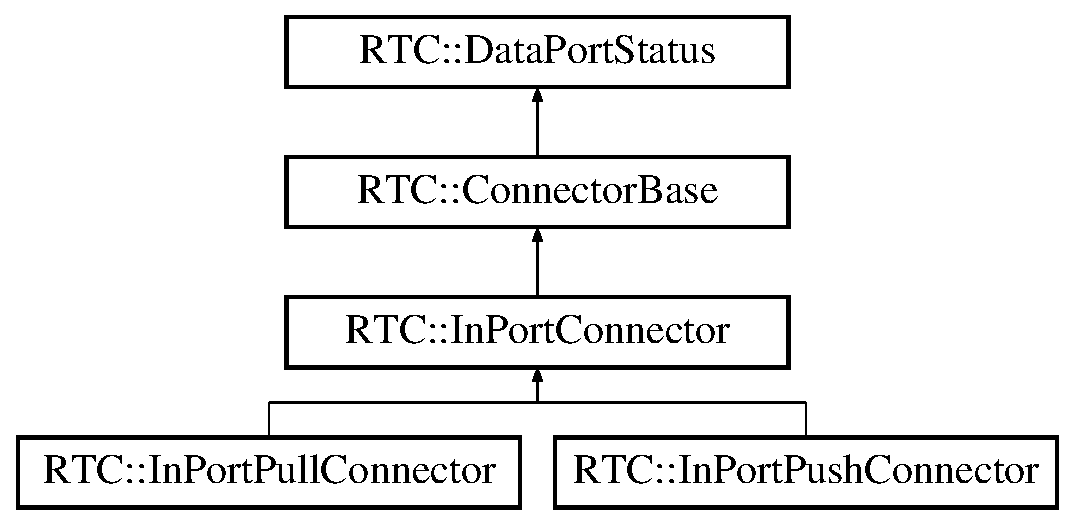
\includegraphics[height=4cm]{classRTC_1_1InPortConnector}
\end{center}
\end{figure}
\subsection*{Public Member Functions}
\begin{DoxyCompactItemize}
\item 
DATAPORTSTATUS\_\-ENUM {\bf InPortConnector} ({\bf ConnectorInfo} \&info, {\bf CdrBufferBase} $\ast$buffer)
\begin{DoxyCompactList}\small\item\em Constructor. \item\end{DoxyCompactList}\item 
virtual {\bf $\sim$InPortConnector} ()
\begin{DoxyCompactList}\small\item\em Destructor. \item\end{DoxyCompactList}\item 
virtual const {\bf ConnectorInfo} \& {\bf profile} ()
\begin{DoxyCompactList}\small\item\em Getting \doxyref{ConnectorInfo}{p.}{classRTC_1_1ConnectorInfo}. \item\end{DoxyCompactList}\item 
virtual const char $\ast$ {\bf id} ()
\begin{DoxyCompactList}\small\item\em Getting Connector ID. \item\end{DoxyCompactList}\item 
virtual const char $\ast$ {\bf name} ()
\begin{DoxyCompactList}\small\item\em Getting Connector name. \item\end{DoxyCompactList}\item 
virtual ReturnCode {\bf disconnect} ()=0
\begin{DoxyCompactList}\small\item\em Disconnect connection. \item\end{DoxyCompactList}\item 
virtual {\bf CdrBufferBase} $\ast$ {\bf getBuffer} ()
\begin{DoxyCompactList}\small\item\em Getting Buffer. \item\end{DoxyCompactList}\item 
virtual ReturnCode {\bf read} (cdrMemoryStream \&data)=0
\begin{DoxyCompactList}\small\item\em Destructor. \item\end{DoxyCompactList}\item 
virtual void {\bf setEndian} (const bool endian\_\-type)
\begin{DoxyCompactList}\small\item\em Setting an endian type. \item\end{DoxyCompactList}\item 
virtual bool {\bf isLittleEndian} ()
\begin{DoxyCompactList}\small\item\em Whether this connector's endian is little. \item\end{DoxyCompactList}\end{DoxyCompactItemize}
\subsection*{Protected Attributes}
\begin{DoxyCompactItemize}
\item 
{\bf Logger} {\bf rtclog}
\begin{DoxyCompactList}\small\item\em \doxyref{Logger}{p.}{classRTC_1_1Logger} stream. \item\end{DoxyCompactList}\item 
{\bf ConnectorInfo} {\bf m\_\-profile}
\begin{DoxyCompactList}\small\item\em \doxyref{ConnectorInfo}{p.}{classRTC_1_1ConnectorInfo}. \item\end{DoxyCompactList}\item 
{\bf CdrBufferBase} $\ast$ {\bf m\_\-buffer}
\begin{DoxyCompactList}\small\item\em Connector's buffer. \item\end{DoxyCompactList}\item 
bool {\bf m\_\-littleEndian}
\begin{DoxyCompactList}\small\item\em Connected Endian. \item\end{DoxyCompactList}\end{DoxyCompactItemize}


\subsection{Detailed Description}
\doxyref{InPortConnector}{p.}{classRTC_1_1InPortConnector} base class. The base class to derive subclasses for InPort's Push/Pull Connectors

\begin{DoxySince}{Since}
1.0.0 
\end{DoxySince}


\subsection{Constructor \& Destructor Documentation}
\index{RTC::InPortConnector@{RTC::InPortConnector}!InPortConnector@{InPortConnector}}
\index{InPortConnector@{InPortConnector}!RTC::InPortConnector@{RTC::InPortConnector}}
\subsubsection[{InPortConnector}]{\setlength{\rightskip}{0pt plus 5cm}DATAPORTSTATUS\_\-ENUM RTC::InPortConnector::InPortConnector ({\bf ConnectorInfo} \& {\em info}, \/  {\bf CdrBufferBase} $\ast$ {\em buffer})}\label{classRTC_1_1InPortConnector_a5817248420e91c6bc5c939d0e48cd417}


Constructor. 


\begin{DoxyParams}{Parameters}
\item[{\em info}]\doxyref{ConnectorInfo}{p.}{classRTC_1_1ConnectorInfo} object which includes connection information \item[{\em buffer}]A pointer to the buffer of the connector \end{DoxyParams}
\index{RTC::InPortConnector@{RTC::InPortConnector}!$\sim$InPortConnector@{$\sim$InPortConnector}}
\index{$\sim$InPortConnector@{$\sim$InPortConnector}!RTC::InPortConnector@{RTC::InPortConnector}}
\subsubsection[{$\sim$InPortConnector}]{\setlength{\rightskip}{0pt plus 5cm}virtual RTC::InPortConnector::$\sim$InPortConnector ()\hspace{0.3cm}{\ttfamily  [virtual]}}\label{classRTC_1_1InPortConnector_aad8160823b8a719fd80bdfb752deddb5}


Destructor. 



\subsection{Member Function Documentation}
\index{RTC::InPortConnector@{RTC::InPortConnector}!disconnect@{disconnect}}
\index{disconnect@{disconnect}!RTC::InPortConnector@{RTC::InPortConnector}}
\subsubsection[{disconnect}]{\setlength{\rightskip}{0pt plus 5cm}virtual ReturnCode RTC::InPortConnector::disconnect ()\hspace{0.3cm}{\ttfamily  [pure virtual]}}\label{classRTC_1_1InPortConnector_a8677105bbf5ae5ed3e79dc3b057ea0b9}


Disconnect connection. 

This operation disconnect this connection

\begin{DoxyReturn}{Returns}
ReturnCode 
\end{DoxyReturn}


Implements {\bf RTC::ConnectorBase} \doxyref{}{p.}{classRTC_1_1ConnectorBase_a17b1e3bb26ccb844ef2952661977768c}.



Implemented in {\bf RTC::InPortPullConnector} \doxyref{}{p.}{classRTC_1_1InPortPullConnector_a74e8c2fbfdbbacd1d3a67b4017b993df}, and {\bf RTC::InPortPushConnector} \doxyref{}{p.}{classRTC_1_1InPortPushConnector_afb5920eabaa874b43bc900348a2fb2ad}.

\index{RTC::InPortConnector@{RTC::InPortConnector}!getBuffer@{getBuffer}}
\index{getBuffer@{getBuffer}!RTC::InPortConnector@{RTC::InPortConnector}}
\subsubsection[{getBuffer}]{\setlength{\rightskip}{0pt plus 5cm}virtual {\bf CdrBufferBase}$\ast$ RTC::InPortConnector::getBuffer ()\hspace{0.3cm}{\ttfamily  [virtual]}}\label{classRTC_1_1InPortConnector_a7a2e6e83f1c50892632b5e23bf2f8ec6}


Getting Buffer. 

This operation returns this connector's buffer

\begin{DoxyReturn}{Returns}
A pointer to the buffer owned by this connector 
\end{DoxyReturn}


Implements {\bf RTC::ConnectorBase} \doxyref{}{p.}{classRTC_1_1ConnectorBase_ad06710a5e9e1862ed50d4a4411c2927d}.

\index{RTC::InPortConnector@{RTC::InPortConnector}!id@{id}}
\index{id@{id}!RTC::InPortConnector@{RTC::InPortConnector}}
\subsubsection[{id}]{\setlength{\rightskip}{0pt plus 5cm}virtual const char$\ast$ RTC::InPortConnector::id ()\hspace{0.3cm}{\ttfamily  [virtual]}}\label{classRTC_1_1InPortConnector_af497212651998eaef0c38913d4762f52}


Getting Connector ID. 

This operation returns Connector ID

\begin{DoxyReturn}{Returns}
A pointer to the connector id string 
\end{DoxyReturn}


Implements {\bf RTC::ConnectorBase} \doxyref{}{p.}{classRTC_1_1ConnectorBase_ae2cc57833a7e28f0e605222ecb63e219}.

\index{RTC::InPortConnector@{RTC::InPortConnector}!isLittleEndian@{isLittleEndian}}
\index{isLittleEndian@{isLittleEndian}!RTC::InPortConnector@{RTC::InPortConnector}}
\subsubsection[{isLittleEndian}]{\setlength{\rightskip}{0pt plus 5cm}virtual bool RTC::InPortConnector::isLittleEndian ()\hspace{0.3cm}{\ttfamily  [virtual]}}\label{classRTC_1_1InPortConnector_ac7e308f77f6b5210694320ebab0e0651}


Whether this connector's endian is little. 

This operation returns whether the connector's endian is little or not.

\begin{DoxyReturn}{Returns}
true: little endian, false: big endian 
\end{DoxyReturn}
\index{RTC::InPortConnector@{RTC::InPortConnector}!name@{name}}
\index{name@{name}!RTC::InPortConnector@{RTC::InPortConnector}}
\subsubsection[{name}]{\setlength{\rightskip}{0pt plus 5cm}virtual const char$\ast$ RTC::InPortConnector::name ()\hspace{0.3cm}{\ttfamily  [virtual]}}\label{classRTC_1_1InPortConnector_abb9dd2bf3f81d132a2a3eb4f31ff461d}


Getting Connector name. 

This operation returns Connector name

\begin{DoxyReturn}{Returns}
A pointer to the connector's name string 
\end{DoxyReturn}


Implements {\bf RTC::ConnectorBase} \doxyref{}{p.}{classRTC_1_1ConnectorBase_a73e002174dc02ec4830c624e7fd96b43}.

\index{RTC::InPortConnector@{RTC::InPortConnector}!profile@{profile}}
\index{profile@{profile}!RTC::InPortConnector@{RTC::InPortConnector}}
\subsubsection[{profile}]{\setlength{\rightskip}{0pt plus 5cm}virtual const {\bf ConnectorInfo}\& RTC::InPortConnector::profile ()\hspace{0.3cm}{\ttfamily  [virtual]}}\label{classRTC_1_1InPortConnector_ade653239f3932f5968ee818ecfd53354}


Getting \doxyref{ConnectorInfo}{p.}{classRTC_1_1ConnectorInfo}. 

This operation returns \doxyref{ConnectorInfo}{p.}{classRTC_1_1ConnectorInfo}

\begin{DoxyReturn}{Returns}
\doxyref{ConnectorInfo}{p.}{classRTC_1_1ConnectorInfo} object which is owned by this connector 
\end{DoxyReturn}


Implements {\bf RTC::ConnectorBase} \doxyref{}{p.}{classRTC_1_1ConnectorBase_a8bd2e9cbd6a9341ec4c97416dcf981c7}.

\index{RTC::InPortConnector@{RTC::InPortConnector}!read@{read}}
\index{read@{read}!RTC::InPortConnector@{RTC::InPortConnector}}
\subsubsection[{read}]{\setlength{\rightskip}{0pt plus 5cm}virtual ReturnCode RTC::InPortConnector::read (cdrMemoryStream \& {\em data})\hspace{0.3cm}{\ttfamily  [pure virtual]}}\label{classRTC_1_1InPortConnector_a2ffc997f36cb6549029852484327bffd}


Destructor. 

The read function to read data from buffer to \doxyref{InPort}{p.}{classRTC_1_1InPort}


\begin{DoxyParams}{Parameters}
\item[{\em data}]A reference to a variable to which data from this connector is stored. \end{DoxyParams}
\begin{DoxyReturn}{Returns}
ReturnCode 
\end{DoxyReturn}


Implemented in {\bf RTC::InPortPullConnector} \doxyref{}{p.}{classRTC_1_1InPortPullConnector_ac2bfcf970c6c0422e279af7d3b638efd}, and {\bf RTC::InPortPushConnector} \doxyref{}{p.}{classRTC_1_1InPortPushConnector_a1403a79f0e0ce7d6c34b4385db6ed8ef}.

\index{RTC::InPortConnector@{RTC::InPortConnector}!setEndian@{setEndian}}
\index{setEndian@{setEndian}!RTC::InPortConnector@{RTC::InPortConnector}}
\subsubsection[{setEndian}]{\setlength{\rightskip}{0pt plus 5cm}virtual void RTC::InPortConnector::setEndian (const bool {\em endian\_\-type})\hspace{0.3cm}{\ttfamily  [virtual]}}\label{classRTC_1_1InPortConnector_a2349abc81262854781949e9d376cd109}


Setting an endian type. 

This operation set this connector's endian type


\begin{DoxyParams}{Parameters}
\item[{\em endian\_\-type}]true: little, false: big \end{DoxyParams}


\subsection{Member Data Documentation}
\index{RTC::InPortConnector@{RTC::InPortConnector}!m\_\-buffer@{m\_\-buffer}}
\index{m\_\-buffer@{m\_\-buffer}!RTC::InPortConnector@{RTC::InPortConnector}}
\subsubsection[{m\_\-buffer}]{\setlength{\rightskip}{0pt plus 5cm}{\bf CdrBufferBase}$\ast$ {\bf RTC::InPortConnector::m\_\-buffer}\hspace{0.3cm}{\ttfamily  [protected]}}\label{classRTC_1_1InPortConnector_aef89e379b8b4045f26bb36cc3c537d70}


Connector's buffer. 

\index{RTC::InPortConnector@{RTC::InPortConnector}!m\_\-littleEndian@{m\_\-littleEndian}}
\index{m\_\-littleEndian@{m\_\-littleEndian}!RTC::InPortConnector@{RTC::InPortConnector}}
\subsubsection[{m\_\-littleEndian}]{\setlength{\rightskip}{0pt plus 5cm}bool {\bf RTC::InPortConnector::m\_\-littleEndian}\hspace{0.3cm}{\ttfamily  [protected]}}\label{classRTC_1_1InPortConnector_a5cb0e047a379c1d4c4ee1e1fea4e9663}


Connected Endian. 

\index{RTC::InPortConnector@{RTC::InPortConnector}!m\_\-profile@{m\_\-profile}}
\index{m\_\-profile@{m\_\-profile}!RTC::InPortConnector@{RTC::InPortConnector}}
\subsubsection[{m\_\-profile}]{\setlength{\rightskip}{0pt plus 5cm}{\bf ConnectorInfo} {\bf RTC::InPortConnector::m\_\-profile}\hspace{0.3cm}{\ttfamily  [protected]}}\label{classRTC_1_1InPortConnector_a8983dceedb2ae10a2f583ab9632f4337}


\doxyref{ConnectorInfo}{p.}{classRTC_1_1ConnectorInfo}. 

\index{RTC::InPortConnector@{RTC::InPortConnector}!rtclog@{rtclog}}
\index{rtclog@{rtclog}!RTC::InPortConnector@{RTC::InPortConnector}}
\subsubsection[{rtclog}]{\setlength{\rightskip}{0pt plus 5cm}{\bf Logger} {\bf RTC::InPortConnector::rtclog}\hspace{0.3cm}{\ttfamily  [protected]}}\label{classRTC_1_1InPortConnector_a823551eac7e254552246921cca0c4c92}


\doxyref{Logger}{p.}{classRTC_1_1Logger} stream. 


\section{RTC::InPortConsumer Class Reference}
\label{classRTC_1_1InPortConsumer}\index{RTC::InPortConsumer@{RTC::InPortConsumer}}


\doxyref{InPortConsumer}{p.}{classRTC_1_1InPortConsumer} abstract class.  




{\ttfamily \#include $<$InPortConsumer.h$>$}

Inheritance diagram for RTC::InPortConsumer:\begin{figure}[H]
\begin{center}
\leavevmode
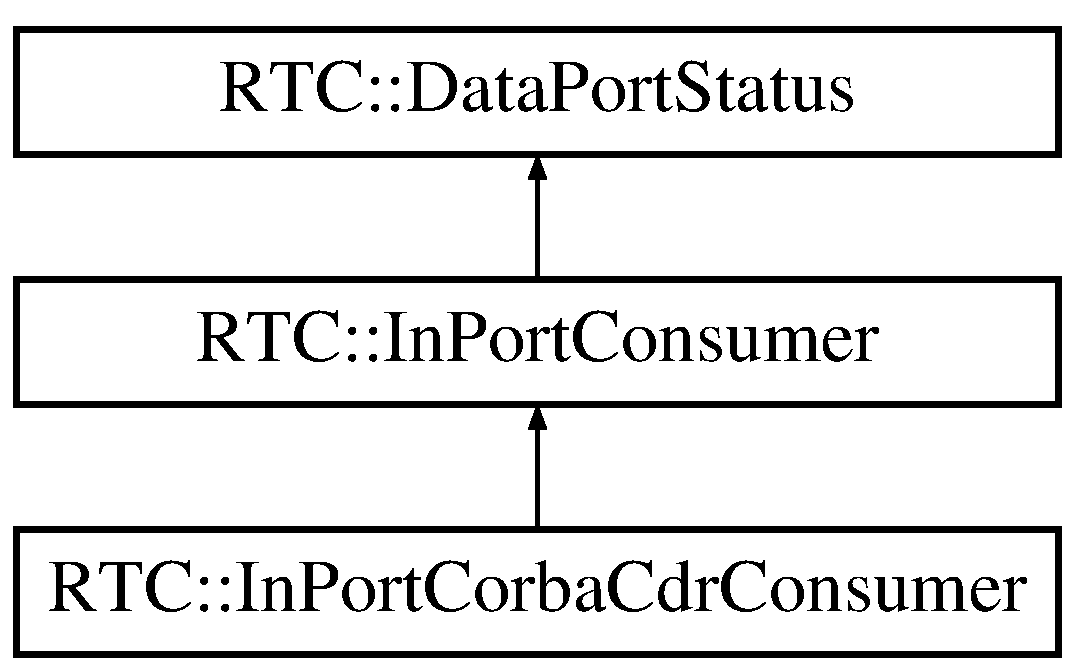
\includegraphics[height=3cm]{classRTC_1_1InPortConsumer}
\end{center}
\end{figure}
\subsection*{Classes}
\begin{DoxyCompactItemize}
\item 
struct {\bf publishInterfaceProfileFunc}
\begin{DoxyCompactList}\small\item\em Functor to publish interface profile. \item\end{DoxyCompactList}\item 
struct {\bf subscribeInterfaceFunc}
\begin{DoxyCompactList}\small\item\em Functor to publish interface profile. \item\end{DoxyCompactList}\end{DoxyCompactItemize}
\subsection*{Public Member Functions}
\begin{DoxyCompactItemize}
\item 
virtual DATAPORTSTATUS\_\-ENUM {\bf $\sim$InPortConsumer} (void)
\begin{DoxyCompactList}\small\item\em Destructor. \item\end{DoxyCompactList}\item 
virtual void {\bf init} ({\bf coil::Properties} \&prop)=0
\begin{DoxyCompactList}\small\item\em Initializing configuration. \item\end{DoxyCompactList}\item 
virtual ReturnCode {\bf put} (const cdrMemoryStream \&data)=0
\begin{DoxyCompactList}\small\item\em Send data to the destination port. \item\end{DoxyCompactList}\item 
virtual void {\bf publishInterfaceProfile} (SDOPackage::NVList \&properties)=0
\begin{DoxyCompactList}\small\item\em Publish InterfaceProfile information. \item\end{DoxyCompactList}\item 
virtual bool {\bf subscribeInterface} (const SDOPackage::NVList \&properties)=0
\begin{DoxyCompactList}\small\item\em Subscribe the data send notification. \item\end{DoxyCompactList}\item 
virtual void {\bf unsubscribeInterface} (const SDOPackage::NVList \&properties)=0
\begin{DoxyCompactList}\small\item\em Unsubscribe the data send notification. \item\end{DoxyCompactList}\end{DoxyCompactItemize}


\subsection{Detailed Description}
\doxyref{InPortConsumer}{p.}{classRTC_1_1InPortConsumer} abstract class. This is the abstract interface class for the input port \doxyref{Consumer}{p.}{classConsumer}. Concrete classes must implement the following pure virtual functions.
\begin{DoxyItemize}
\item push(): Send data
\item clone(): Copy ports
\item \doxyref{subscribeInterface()}{p.}{classRTC_1_1InPortConsumer_a63073caab2216e2686b34d2c8901c591}: Subscribe the data send notification
\item \doxyref{unsubscribeInterface()}{p.}{classRTC_1_1InPortConsumer_a59530bf39fca610e2c7136700a214aab}: Unsubscribe the data send notification
\end{DoxyItemize}

\begin{DoxySince}{Since}
0.4.0 
\end{DoxySince}


\subsection{Constructor \& Destructor Documentation}
\index{RTC::InPortConsumer@{RTC::InPortConsumer}!$\sim$InPortConsumer@{$\sim$InPortConsumer}}
\index{$\sim$InPortConsumer@{$\sim$InPortConsumer}!RTC::InPortConsumer@{RTC::InPortConsumer}}
\subsubsection[{$\sim$InPortConsumer}]{\setlength{\rightskip}{0pt plus 5cm}virtual DATAPORTSTATUS\_\-ENUM RTC::InPortConsumer::$\sim$InPortConsumer (void)\hspace{0.3cm}{\ttfamily  [inline, virtual]}}\label{classRTC_1_1InPortConsumer_a6a6d7b589839aa3d42129198f7c7e2e5}


Destructor. 

Destructor 

\subsection{Member Function Documentation}
\index{RTC::InPortConsumer@{RTC::InPortConsumer}!init@{init}}
\index{init@{init}!RTC::InPortConsumer@{RTC::InPortConsumer}}
\subsubsection[{init}]{\setlength{\rightskip}{0pt plus 5cm}virtual void RTC::InPortConsumer::init ({\bf coil::Properties} \& {\em prop})\hspace{0.3cm}{\ttfamily  [pure virtual]}}\label{classRTC_1_1InPortConsumer_a70772c84fa42d6108e30c0f52a9674d5}


Initializing configuration. 

This operation would be called to configure this consumer in initialization. 

Implemented in {\bf RTC::InPortCorbaCdrConsumer} \doxyref{}{p.}{classRTC_1_1InPortCorbaCdrConsumer_a5682cf80be88cfbb6ab238e7b3733686}.

\index{RTC::InPortConsumer@{RTC::InPortConsumer}!publishInterfaceProfile@{publishInterfaceProfile}}
\index{publishInterfaceProfile@{publishInterfaceProfile}!RTC::InPortConsumer@{RTC::InPortConsumer}}
\subsubsection[{publishInterfaceProfile}]{\setlength{\rightskip}{0pt plus 5cm}virtual void RTC::InPortConsumer::publishInterfaceProfile (SDOPackage::NVList \& {\em properties})\hspace{0.3cm}{\ttfamily  [pure virtual]}}\label{classRTC_1_1InPortConsumer_a1bb34ea50047ecf1b2642fc61192d40b}


Publish InterfaceProfile information. 

Publish interfaceProfile information. Check the dataport.interface\_\-type value of the NameValue object specified by an argument in property information and get information only when the interface type of the specified port is matched.


\begin{DoxyParams}{Parameters}
\item[{\em properties}]Properties to get InterfaceProfile information \end{DoxyParams}


Implemented in {\bf RTC::InPortCorbaCdrConsumer} \doxyref{}{p.}{classRTC_1_1InPortCorbaCdrConsumer_aa71ca4621080b782a09a640f18daa2e9}.



Referenced by RTC::InPortConsumer::publishInterfaceProfileFunc::operator()().

\index{RTC::InPortConsumer@{RTC::InPortConsumer}!put@{put}}
\index{put@{put}!RTC::InPortConsumer@{RTC::InPortConsumer}}
\subsubsection[{put}]{\setlength{\rightskip}{0pt plus 5cm}virtual ReturnCode RTC::InPortConsumer::put (const cdrMemoryStream \& {\em data})\hspace{0.3cm}{\ttfamily  [pure virtual]}}\label{classRTC_1_1InPortConsumer_a7868875b611a5dde0db3d0fcdf5703e5}


Send data to the destination port. 

Pure virtual function to send data to the destination port.

This function might the following return codes


\begin{DoxyItemize}
\item PORT\_\-OK: Normal return
\item PORT\_\-ERROR: Error occurred in data transfer process
\item SEND\_\-FULL: Buffer full although \doxyref{OutPort}{p.}{classRTC_1_1OutPort} tried to send data
\item SEND\_\-TIMEOUT: Timeout although \doxyref{OutPort}{p.}{classRTC_1_1OutPort} tried to send data
\item CONNECTION\_\-LOST: Connection lost
\item UNKNOWN\_\-ERROR: Unknown error 
\end{DoxyItemize}

Implemented in {\bf RTC::InPortCorbaCdrConsumer} \doxyref{}{p.}{classRTC_1_1InPortCorbaCdrConsumer_ab910b2bf2a841c2c11bce50e75d36abb}.

\index{RTC::InPortConsumer@{RTC::InPortConsumer}!subscribeInterface@{subscribeInterface}}
\index{subscribeInterface@{subscribeInterface}!RTC::InPortConsumer@{RTC::InPortConsumer}}
\subsubsection[{subscribeInterface}]{\setlength{\rightskip}{0pt plus 5cm}virtual bool RTC::InPortConsumer::subscribeInterface (const SDOPackage::NVList \& {\em properties})\hspace{0.3cm}{\ttfamily  [pure virtual]}}\label{classRTC_1_1InPortConsumer_a63073caab2216e2686b34d2c8901c591}


Subscribe the data send notification. 

Pure virtual function to subscribe the data send notification based on specified property information.


\begin{DoxyParams}{Parameters}
\item[{\em properties}]Properties for reference when subscribing\end{DoxyParams}
\begin{DoxyReturn}{Returns}
Subscription result 
\end{DoxyReturn}


Implemented in {\bf RTC::InPortCorbaCdrConsumer} \doxyref{}{p.}{classRTC_1_1InPortCorbaCdrConsumer_a6ca9cba69e9bc1015d79330ed9a56b71}.



Referenced by RTC::InPortConsumer::subscribeInterfaceFunc::operator()().

\index{RTC::InPortConsumer@{RTC::InPortConsumer}!unsubscribeInterface@{unsubscribeInterface}}
\index{unsubscribeInterface@{unsubscribeInterface}!RTC::InPortConsumer@{RTC::InPortConsumer}}
\subsubsection[{unsubscribeInterface}]{\setlength{\rightskip}{0pt plus 5cm}virtual void RTC::InPortConsumer::unsubscribeInterface (const SDOPackage::NVList \& {\em properties})\hspace{0.3cm}{\ttfamily  [pure virtual]}}\label{classRTC_1_1InPortConsumer_a59530bf39fca610e2c7136700a214aab}


Unsubscribe the data send notification. 

Pure virtual function to unsubscribe the data send notification.


\begin{DoxyParams}{Parameters}
\item[{\em properties}]Properties for reference when unsubscribing \end{DoxyParams}


Implemented in {\bf RTC::InPortCorbaCdrConsumer} \doxyref{}{p.}{classRTC_1_1InPortCorbaCdrConsumer_a6e297f6ebc3dae7b547e1ec8af06ee9f}.


\section{クラス RTC::InPortCorbaCdrConsumer}
\label{classRTC_1_1InPortCorbaCdrConsumer}\index{RTC::InPortCorbaCdrConsumer@{RTC::InPortCorbaCdrConsumer}}


\doxyref{InPortCorbaCdrConsumer}{p.}{classRTC_1_1InPortCorbaCdrConsumer} クラス.  




{\ttfamily \#include $<$InPortCorbaCdrConsumer.h$>$}

RTC::InPortCorbaCdrConsumerに対する継承グラフ\begin{figure}[H]
\begin{center}
\leavevmode
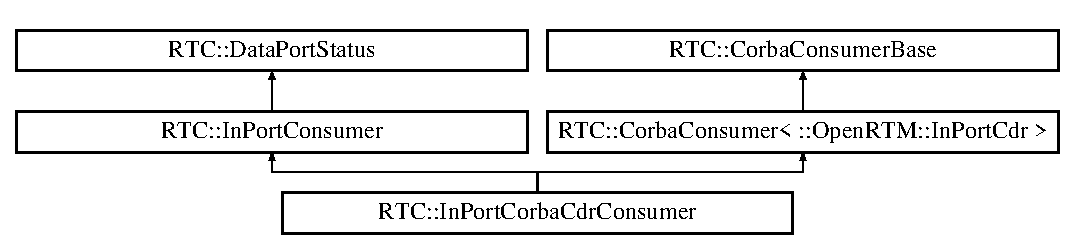
\includegraphics[height=2.90657cm]{classRTC_1_1InPortCorbaCdrConsumer}
\end{center}
\end{figure}
\subsection*{Public メソッド}
\begin{DoxyCompactItemize}
\item 
DATAPORTSTATUS\_\-ENUM {\bf InPortCorbaCdrConsumer} (void)
\begin{DoxyCompactList}\small\item\em コンストラクタ \item\end{DoxyCompactList}\item 
virtual {\bf $\sim$InPortCorbaCdrConsumer} (void)
\item 
virtual void {\bf init} ({\bf coil::Properties} \&prop)
\begin{DoxyCompactList}\small\item\em 設定初期化 \item\end{DoxyCompactList}\item 
virtual ReturnCode {\bf put} (const cdrMemoryStream \&data)
\begin{DoxyCompactList}\small\item\em 接続先へのデータ送信 \item\end{DoxyCompactList}\item 
virtual void {\bf publishInterfaceProfile} (SDOPackage::NVList \&properties)
\begin{DoxyCompactList}\small\item\em InterfaceProfile情報を公開する. \item\end{DoxyCompactList}\item 
virtual bool {\bf subscribeInterface} (const SDOPackage::NVList \&properties)
\begin{DoxyCompactList}\small\item\em データ送信通知への登録 \item\end{DoxyCompactList}\item 
virtual void {\bf unsubscribeInterface} (const SDOPackage::NVList \&properties)
\begin{DoxyCompactList}\small\item\em データ送信通知からの登録解除 \item\end{DoxyCompactList}\end{DoxyCompactItemize}


\subsection{説明}
\doxyref{InPortCorbaCdrConsumer}{p.}{classRTC_1_1InPortCorbaCdrConsumer} クラス. \doxyref{InPortConsumer}{p.}{classRTC_1_1InPortConsumer}

データ転送に CORBA の OpenRTM::InPortCdr インターフェースを利用し た、push 型データフロー型を実現する \doxyref{InPort}{p.}{classRTC_1_1InPort} コンシューマクラス。

\begin{DoxySince}{から}
0.4.0 
\end{DoxySince}


\subsection{コンストラクタとデストラクタ}
\index{RTC::InPortCorbaCdrConsumer@{RTC::InPortCorbaCdrConsumer}!InPortCorbaCdrConsumer@{InPortCorbaCdrConsumer}}
\index{InPortCorbaCdrConsumer@{InPortCorbaCdrConsumer}!RTC::InPortCorbaCdrConsumer@{RTC::InPortCorbaCdrConsumer}}
\subsubsection[{InPortCorbaCdrConsumer}]{\setlength{\rightskip}{0pt plus 5cm}DATAPORTSTATUS\_\-ENUM RTC::InPortCorbaCdrConsumer::InPortCorbaCdrConsumer (void)}\label{classRTC_1_1InPortCorbaCdrConsumer_a23aa65c030756eac8f28edb006d2a2ab}


コンストラクタ 

コンストラクタ


\begin{DoxyParams}{引数}
\item[{\em buffer}]当該コンシューマに割り当てるバッファオブジェクト \end{DoxyParams}
\index{RTC::InPortCorbaCdrConsumer@{RTC::InPortCorbaCdrConsumer}!$\sim$InPortCorbaCdrConsumer@{$\sim$InPortCorbaCdrConsumer}}
\index{$\sim$InPortCorbaCdrConsumer@{$\sim$InPortCorbaCdrConsumer}!RTC::InPortCorbaCdrConsumer@{RTC::InPortCorbaCdrConsumer}}
\subsubsection[{$\sim$InPortCorbaCdrConsumer}]{\setlength{\rightskip}{0pt plus 5cm}virtual RTC::InPortCorbaCdrConsumer::$\sim$InPortCorbaCdrConsumer (void)\hspace{0.3cm}{\ttfamily  [virtual]}}\label{classRTC_1_1InPortCorbaCdrConsumer_a8822e5bb854e1936fc1f8f19517a8bd3}
デストラクタ 

\subsection{関数}
\index{RTC::InPortCorbaCdrConsumer@{RTC::InPortCorbaCdrConsumer}!init@{init}}
\index{init@{init}!RTC::InPortCorbaCdrConsumer@{RTC::InPortCorbaCdrConsumer}}
\subsubsection[{init}]{\setlength{\rightskip}{0pt plus 5cm}virtual void RTC::InPortCorbaCdrConsumer::init ({\bf coil::Properties} \& {\em prop})\hspace{0.3cm}{\ttfamily  [virtual]}}\label{classRTC_1_1InPortCorbaCdrConsumer_a5682cf80be88cfbb6ab238e7b3733686}


設定初期化 

InPortConsumerの各種設定を行う。実装クラスでは、与えられた Propertiesから必要な情報を取得して各種設定を行う。この \doxyref{init()}{p.}{classRTC_1_1InPortCorbaCdrConsumer_a5682cf80be88cfbb6ab238e7b3733686} 関 数は、InPortProvider生成直後および、接続時にそれぞれ呼ばれる可 能性がある。したがって、この関数は複数回呼ばれることを想定して記 述されるべきである。


\begin{DoxyParams}{引数}
\item[{\em prop}]設定情報 \end{DoxyParams}


{\bf RTC::InPortConsumer} \doxyref{}{p.}{classRTC_1_1InPortConsumer_a70772c84fa42d6108e30c0f52a9674d5}を実装しています。

\index{RTC::InPortCorbaCdrConsumer@{RTC::InPortCorbaCdrConsumer}!publishInterfaceProfile@{publishInterfaceProfile}}
\index{publishInterfaceProfile@{publishInterfaceProfile}!RTC::InPortCorbaCdrConsumer@{RTC::InPortCorbaCdrConsumer}}
\subsubsection[{publishInterfaceProfile}]{\setlength{\rightskip}{0pt plus 5cm}virtual void RTC::InPortCorbaCdrConsumer::publishInterfaceProfile (SDOPackage::NVList \& {\em properties})\hspace{0.3cm}{\ttfamily  [virtual]}}\label{classRTC_1_1InPortCorbaCdrConsumer_aa71ca4621080b782a09a640f18daa2e9}


InterfaceProfile情報を公開する. 

InterfaceProfile情報を公開する。 引数で指定するプロパティ情報内の NameValue オブジェクトの dataport.interface\_\-type 値を調べ、当該ポートに設定されている インターフェースタイプと一致する場合のみ情報を取得する。


\begin{DoxyParams}{引数}
\item[{\em properties}]InterfaceProfile情報を受け取るプロパティ \end{DoxyParams}


{\bf RTC::InPortConsumer} \doxyref{}{p.}{classRTC_1_1InPortConsumer_a1bb34ea50047ecf1b2642fc61192d40b}を実装しています。

\index{RTC::InPortCorbaCdrConsumer@{RTC::InPortCorbaCdrConsumer}!put@{put}}
\index{put@{put}!RTC::InPortCorbaCdrConsumer@{RTC::InPortCorbaCdrConsumer}}
\subsubsection[{put}]{\setlength{\rightskip}{0pt plus 5cm}virtual ReturnCode RTC::InPortCorbaCdrConsumer::put (const cdrMemoryStream \& {\em data})\hspace{0.3cm}{\ttfamily  [virtual]}}\label{classRTC_1_1InPortCorbaCdrConsumer_ab910b2bf2a841c2c11bce50e75d36abb}


接続先へのデータ送信 

接続先のポートへデータを送信するための純粋仮想関数。

この関数は、以下のリターンコードを返す。


\begin{DoxyItemize}
\item PORT\_\-OK: 正常終了。
\item PORT\_\-ERROR: データ送信の過程で何らかのエラーが発生した。
\item SEND\_\-FULL: データを送信したが、相手側バッファがフルだった。
\item SEND\_\-TIMEOUT: データを送信したが、相手側バッファがタイムアウトした。
\item UNKNOWN\_\-ERROR: 原因不明のエラー
\end{DoxyItemize}


\begin{DoxyParams}{引数}
\item[{\em data}]送信するデータ \end{DoxyParams}
\begin{DoxyReturn}{戻り値}
リターンコード 
\end{DoxyReturn}


{\bf RTC::InPortConsumer} \doxyref{}{p.}{classRTC_1_1InPortConsumer_a7868875b611a5dde0db3d0fcdf5703e5}を実装しています。

\index{RTC::InPortCorbaCdrConsumer@{RTC::InPortCorbaCdrConsumer}!subscribeInterface@{subscribeInterface}}
\index{subscribeInterface@{subscribeInterface}!RTC::InPortCorbaCdrConsumer@{RTC::InPortCorbaCdrConsumer}}
\subsubsection[{subscribeInterface}]{\setlength{\rightskip}{0pt plus 5cm}virtual bool RTC::InPortCorbaCdrConsumer::subscribeInterface (const SDOPackage::NVList \& {\em properties})\hspace{0.3cm}{\ttfamily  [virtual]}}\label{classRTC_1_1InPortCorbaCdrConsumer_a6ca9cba69e9bc1015d79330ed9a56b71}


データ送信通知への登録 

指定されたプロパティに基づいて、データ送出通知の受け取りに登録する。


\begin{DoxyParams}{引数}
\item[{\em properties}]登録情報\end{DoxyParams}
\begin{DoxyReturn}{戻り値}
登録処理結果(登録成功:true、登録失敗:false) 
\end{DoxyReturn}


{\bf RTC::InPortConsumer} \doxyref{}{p.}{classRTC_1_1InPortConsumer_a63073caab2216e2686b34d2c8901c591}を実装しています。

\index{RTC::InPortCorbaCdrConsumer@{RTC::InPortCorbaCdrConsumer}!unsubscribeInterface@{unsubscribeInterface}}
\index{unsubscribeInterface@{unsubscribeInterface}!RTC::InPortCorbaCdrConsumer@{RTC::InPortCorbaCdrConsumer}}
\subsubsection[{unsubscribeInterface}]{\setlength{\rightskip}{0pt plus 5cm}virtual void RTC::InPortCorbaCdrConsumer::unsubscribeInterface (const SDOPackage::NVList \& {\em properties})\hspace{0.3cm}{\ttfamily  [virtual]}}\label{classRTC_1_1InPortCorbaCdrConsumer_a6e297f6ebc3dae7b547e1ec8af06ee9f}


データ送信通知からの登録解除 

データ送出通知の受け取りから登録を解除する。


\begin{DoxyParams}{引数}
\item[{\em properties}]登録解除情報 \end{DoxyParams}


{\bf RTC::InPortConsumer} \doxyref{}{p.}{classRTC_1_1InPortConsumer_a59530bf39fca610e2c7136700a214aab}を実装しています。


\section{クラス RTC::InPortCorbaCdrProvider}
\label{classRTC_1_1InPortCorbaCdrProvider}\index{RTC::InPortCorbaCdrProvider@{RTC::InPortCorbaCdrProvider}}


\doxyref{InPortCorbaCdrProvider}{p.}{classRTC_1_1InPortCorbaCdrProvider} クラス.  




{\ttfamily \#include $<$InPortCorbaCdrProvider.h$>$}

RTC::InPortCorbaCdrProviderに対する継承グラフ\begin{figure}[H]
\begin{center}
\leavevmode
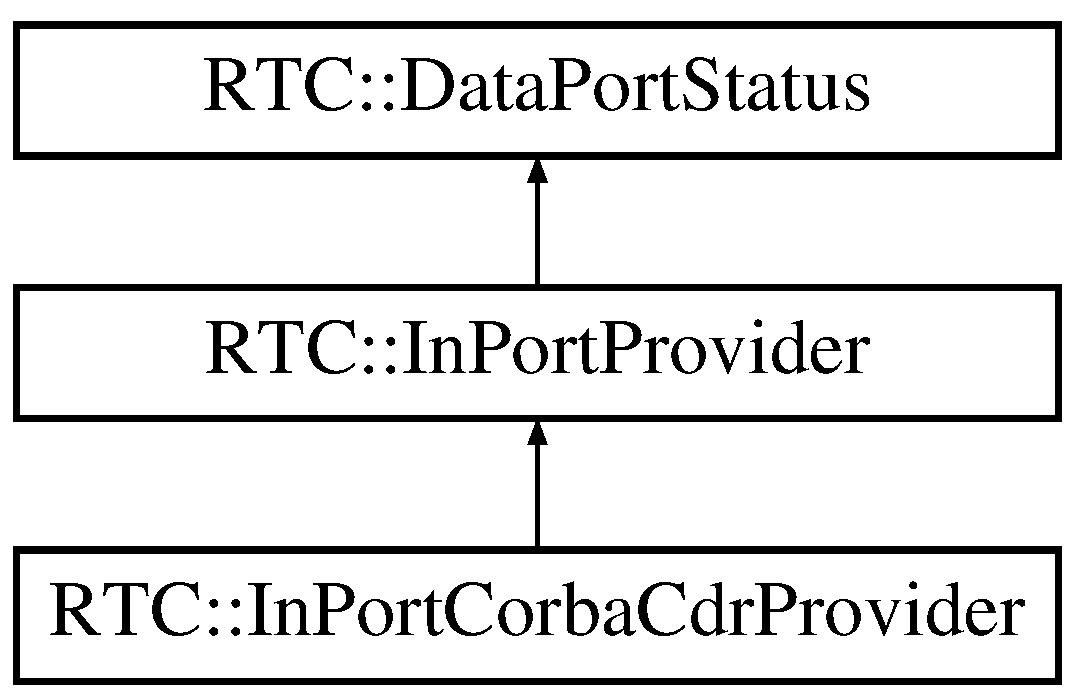
\includegraphics[height=3cm]{classRTC_1_1InPortCorbaCdrProvider}
\end{center}
\end{figure}
\subsection*{Public メソッド}
\begin{DoxyCompactItemize}
\item 
{\bf InPortCorbaCdrProvider} (void)
\item 
virtual {\bf $\sim$InPortCorbaCdrProvider} (void)
\item 
virtual void {\bf init} ({\bf coil::Properties} \&prop)
\begin{DoxyCompactList}\small\item\em 設定初期化 \item\end{DoxyCompactList}\item 
virtual void {\bf setBuffer} ({\bf BufferBase}$<$ cdrMemoryStream $>$ $\ast$buffer)
\begin{DoxyCompactList}\small\item\em バッファをセットする \item\end{DoxyCompactList}\item 
virtual void {\bf setListener} ({\bf ConnectorInfo} \&info, {\bf ConnectorListeners} $\ast$listeners)
\begin{DoxyCompactList}\small\item\em リスナを設定する。 \item\end{DoxyCompactList}\item 
virtual void {\bf setConnector} ({\bf InPortConnector} $\ast$connector)
\begin{DoxyCompactList}\small\item\em Connectorを設定する。. \item\end{DoxyCompactList}\item 
virtual ::OpenRTM::PortStatus {\bf put} (const ::OpenRTM::CdrData \&data)  throw (CORBA::SystemException)
\begin{DoxyCompactList}\small\item\em [CORBA interface] バッファにデータを書き込む \item\end{DoxyCompactList}\end{DoxyCompactItemize}


\subsection{説明}
\doxyref{InPortCorbaCdrProvider}{p.}{classRTC_1_1InPortCorbaCdrProvider} クラス. \doxyref{InPortProvider}{p.}{classRTC_1_1InPortProvider}

データ転送に CORBA の OpenRTM::InPortCdr インターフェースを利用し た、push 型データフロー型を実現する \doxyref{InPort}{p.}{classRTC_1_1InPort} プロバイダクラス。

\begin{DoxySince}{から}
0.4.0 
\end{DoxySince}


\subsection{コンストラクタとデストラクタ}
\index{RTC::InPortCorbaCdrProvider@{RTC::InPortCorbaCdrProvider}!InPortCorbaCdrProvider@{InPortCorbaCdrProvider}}
\index{InPortCorbaCdrProvider@{InPortCorbaCdrProvider}!RTC::InPortCorbaCdrProvider@{RTC::InPortCorbaCdrProvider}}
\subsubsection[{InPortCorbaCdrProvider}]{\setlength{\rightskip}{0pt plus 5cm}RTC::InPortCorbaCdrProvider::InPortCorbaCdrProvider (void)}\label{classRTC_1_1InPortCorbaCdrProvider_abc94c880d3aa109e53a708f95ef46864}
コンストラクタ \index{RTC::InPortCorbaCdrProvider@{RTC::InPortCorbaCdrProvider}!$\sim$InPortCorbaCdrProvider@{$\sim$InPortCorbaCdrProvider}}
\index{$\sim$InPortCorbaCdrProvider@{$\sim$InPortCorbaCdrProvider}!RTC::InPortCorbaCdrProvider@{RTC::InPortCorbaCdrProvider}}
\subsubsection[{$\sim$InPortCorbaCdrProvider}]{\setlength{\rightskip}{0pt plus 5cm}virtual RTC::InPortCorbaCdrProvider::$\sim$InPortCorbaCdrProvider (void)\hspace{0.3cm}{\ttfamily  [virtual]}}\label{classRTC_1_1InPortCorbaCdrProvider_a192fc93998b8635b05c1cbff1274a665}
デストラクタ 

\subsection{関数}
\index{RTC::InPortCorbaCdrProvider@{RTC::InPortCorbaCdrProvider}!init@{init}}
\index{init@{init}!RTC::InPortCorbaCdrProvider@{RTC::InPortCorbaCdrProvider}}
\subsubsection[{init}]{\setlength{\rightskip}{0pt plus 5cm}virtual void RTC::InPortCorbaCdrProvider::init ({\bf coil::Properties} \& {\em prop})\hspace{0.3cm}{\ttfamily  [virtual]}}\label{classRTC_1_1InPortCorbaCdrProvider_a745af48699ac6dff711bb67331210b58}


設定初期化 

\doxyref{InPortCorbaCdrProvider}{p.}{classRTC_1_1InPortCorbaCdrProvider} の各種設定を行う。与えられた Propertiesから必要な情報を取得して各種設定を行う。この \doxyref{init()}{p.}{classRTC_1_1InPortCorbaCdrProvider_a745af48699ac6dff711bb67331210b58} 関 数は、InPortProvider生成直後および、接続時にそれぞれ呼ばれる可 能性がある。したがって、この関数は複数回呼ばれることを想定して記 述されるべきである。


\begin{DoxyParams}{引数}
\item[{\em prop}]設定情報 \end{DoxyParams}


{\bf RTC::InPortProvider} \doxyref{}{p.}{classRTC_1_1InPortProvider_a66c64488543761e1c8874f88fc55ff00}を実装しています。

\index{RTC::InPortCorbaCdrProvider@{RTC::InPortCorbaCdrProvider}!put@{put}}
\index{put@{put}!RTC::InPortCorbaCdrProvider@{RTC::InPortCorbaCdrProvider}}
\subsubsection[{put}]{\setlength{\rightskip}{0pt plus 5cm}virtual ::OpenRTM::PortStatus RTC::InPortCorbaCdrProvider::put (const ::OpenRTM::CdrData \& {\em data})  throw (CORBA::SystemException)}\label{classRTC_1_1InPortCorbaCdrProvider_a51cb31f379b7e95d1787f04bddc947ee}


[CORBA interface] バッファにデータを書き込む 

設定されたバッファにデータを書き込む。


\begin{DoxyParams}{引数}
\item[{\em data}]書込対象データ \end{DoxyParams}
\index{RTC::InPortCorbaCdrProvider@{RTC::InPortCorbaCdrProvider}!setBuffer@{setBuffer}}
\index{setBuffer@{setBuffer}!RTC::InPortCorbaCdrProvider@{RTC::InPortCorbaCdrProvider}}
\subsubsection[{setBuffer}]{\setlength{\rightskip}{0pt plus 5cm}virtual void RTC::InPortCorbaCdrProvider::setBuffer ({\bf BufferBase}$<$ cdrMemoryStream $>$ $\ast$ {\em buffer})\hspace{0.3cm}{\ttfamily  [virtual]}}\label{classRTC_1_1InPortCorbaCdrProvider_ab461b86e9a22b9418a978ba10a74ec72}


バッファをセットする 

\doxyref{OutPortProvider}{p.}{classRTC_1_1OutPortProvider} がデータを取り出すバッファをセットする。 すでにセットされたバッファがある場合、以前のバッファへの ポインタに対して上書きされる。 OutPortProviderはバッファの所有権を仮定していないので、 バッファの削除はユーザの責任で行わなければならない。


\begin{DoxyParams}{引数}
\item[{\em buffer}]OutPortProviderがデータを取り出すバッファへのポインタ \end{DoxyParams}


{\bf RTC::InPortProvider} \doxyref{}{p.}{classRTC_1_1InPortProvider_a67b305bff0ed99a997570286922aa2ea}を実装しています。

\index{RTC::InPortCorbaCdrProvider@{RTC::InPortCorbaCdrProvider}!setConnector@{setConnector}}
\index{setConnector@{setConnector}!RTC::InPortCorbaCdrProvider@{RTC::InPortCorbaCdrProvider}}
\subsubsection[{setConnector}]{\setlength{\rightskip}{0pt plus 5cm}virtual void RTC::InPortCorbaCdrProvider::setConnector ({\bf InPortConnector} $\ast$ {\em connector})\hspace{0.3cm}{\ttfamily  [virtual]}}\label{classRTC_1_1InPortCorbaCdrProvider_a1f6f663d07ea5a3122410160a5a92147}


Connectorを設定する。. 

\doxyref{InPort}{p.}{classRTC_1_1InPort} は接続確立時に \doxyref{InPortConnector}{p.}{classRTC_1_1InPortConnector} オブジェクトを生成し、生 成したオブジェクトのポインタと共にこの関数を呼び出す。所有権は \doxyref{InPort}{p.}{classRTC_1_1InPort} が保持するので \doxyref{InPortProvider}{p.}{classRTC_1_1InPortProvider} は \doxyref{InPortConnector}{p.}{classRTC_1_1InPortConnector} を削 除してはいけない。


\begin{DoxyParams}{引数}
\item[{\em connector}]\doxyref{InPortConnector}{p.}{classRTC_1_1InPortConnector} \end{DoxyParams}


{\bf RTC::InPortProvider} \doxyref{}{p.}{classRTC_1_1InPortProvider_a3f4980d48f7588d6a85c0858f9b1a37e}を実装しています。

\index{RTC::InPortCorbaCdrProvider@{RTC::InPortCorbaCdrProvider}!setListener@{setListener}}
\index{setListener@{setListener}!RTC::InPortCorbaCdrProvider@{RTC::InPortCorbaCdrProvider}}
\subsubsection[{setListener}]{\setlength{\rightskip}{0pt plus 5cm}virtual void RTC::InPortCorbaCdrProvider::setListener ({\bf ConnectorInfo} \& {\em info}, \/  {\bf ConnectorListeners} $\ast$ {\em listeners})\hspace{0.3cm}{\ttfamily  [virtual]}}\label{classRTC_1_1InPortCorbaCdrProvider_a5319ea343145e3b14c9a107724780dff}


リスナを設定する。 

\doxyref{InPort}{p.}{classRTC_1_1InPort} はデータ送信処理における各種イベントに対して特定のリスナ オブジェクトをコールするコールバック機構を提供する。詳細は \doxyref{ConnectorListener.h}{p.}{ConnectorListener_8h} の \doxyref{ConnectorDataListener}{p.}{classRTC_1_1ConnectorDataListener}, \doxyref{ConnectorListener}{p.}{classRTC_1_1ConnectorListener} 等を参照のこと。InPortCorbaCdrProvider では、以下のコールバック が提供される。


\begin{DoxyItemize}
\item ON\_\-BUFFER\_\-WRITE
\item ON\_\-BUFFER\_\-FULL
\item ON\_\-BUFFER\_\-WRITE\_\-TIMEOUT
\item ON\_\-BUFFER\_\-OVERWRITE
\item ON\_\-RECEIVED
\item ON\_\-RECEIVER\_\-FULL
\item ON\_\-RECEIVER\_\-FULL
\item ON\_\-RECEIVER\_\-TIMEOUT
\item ON\_\-RECEIVER\_\-ERROR
\end{DoxyItemize}


\begin{DoxyParams}{引数}
\item[{\em info}]接続情報 \item[{\em listeners}]リスナオブジェクト \end{DoxyParams}


{\bf RTC::InPortProvider} \doxyref{}{p.}{classRTC_1_1InPortProvider_ae3d3833c958440f7d053d52f42b59390}を実装しています。


\section{クラス RTC::InPortProvider}
\label{classRTC_1_1InPortProvider}\index{RTC::InPortProvider@{RTC::InPortProvider}}


{\ttfamily \#include $<$InPortProvider.h$>$}

RTC::InPortProviderに対する継承グラフ\begin{figure}[H]
\begin{center}
\leavevmode
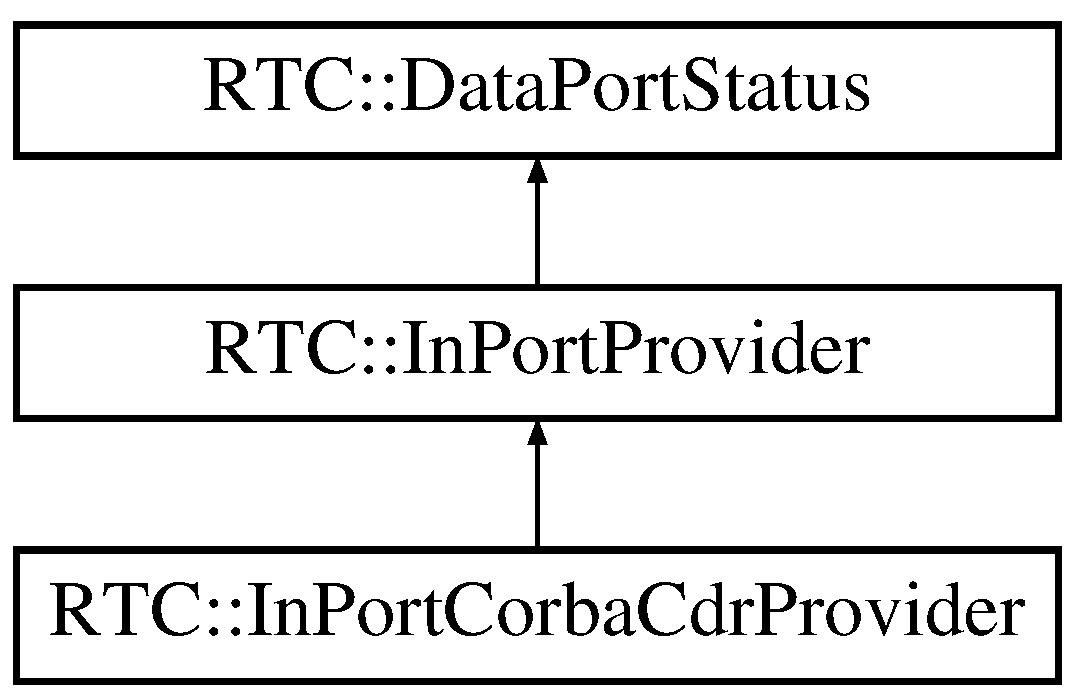
\includegraphics[height=3cm]{classRTC_1_1InPortProvider}
\end{center}
\end{figure}
\subsection*{構成}
\begin{DoxyCompactItemize}
\item 
struct {\bf publishInterfaceFunc}
\begin{DoxyCompactList}\small\item\em インターフェースプロファイルを公開するたのファンクタ \item\end{DoxyCompactList}\item 
struct {\bf publishInterfaceProfileFunc}
\begin{DoxyCompactList}\small\item\em インターフェースプロファイルを公開するたのファンクタ \item\end{DoxyCompactList}\end{DoxyCompactItemize}
\subsection*{Public メソッド}
\begin{DoxyCompactItemize}
\item 
DATAPORTSTATUS\_\-ENUM {\bf InPortProvider} ()
\item 
virtual {\bf $\sim$InPortProvider} (void)
\begin{DoxyCompactList}\small\item\em デストラクタ \item\end{DoxyCompactList}\item 
virtual void {\bf init} ({\bf coil::Properties} \&prop)=0
\begin{DoxyCompactList}\small\item\em 設定初期化 \item\end{DoxyCompactList}\item 
virtual void {\bf setBuffer} ({\bf BufferBase}$<$ cdrMemoryStream $>$ $\ast$buffer)=0
\begin{DoxyCompactList}\small\item\em バッファをセットする \item\end{DoxyCompactList}\item 
virtual void {\bf setListener} ({\bf ConnectorInfo} \&info, {\bf ConnectorListeners} $\ast$listeners)=0
\begin{DoxyCompactList}\small\item\em リスナを設定する。 \item\end{DoxyCompactList}\item 
virtual void {\bf setConnector} ({\bf InPortConnector} $\ast$connector)=0
\begin{DoxyCompactList}\small\item\em Connectorを設定する。. \item\end{DoxyCompactList}\item 
virtual void {\bf publishInterfaceProfile} (SDOPackage::NVList \&properties)
\begin{DoxyCompactList}\small\item\em InterfaceProfile情報を公開する. \item\end{DoxyCompactList}\item 
virtual bool {\bf publishInterface} (SDOPackage::NVList \&properties)
\begin{DoxyCompactList}\small\item\em Interface情報を公開する. \item\end{DoxyCompactList}\end{DoxyCompactItemize}
\subsection*{Protected メソッド}
\begin{DoxyCompactItemize}
\item 
void {\bf setInterfaceType} (const char $\ast$interface\_\-type)
\begin{DoxyCompactList}\small\item\em インタフェースタイプを設定する \item\end{DoxyCompactList}\item 
void {\bf setDataFlowType} (const char $\ast$dataflow\_\-type)
\begin{DoxyCompactList}\small\item\em データフロータイプを設定する \item\end{DoxyCompactList}\item 
void {\bf setSubscriptionType} (const char $\ast$subs\_\-type)
\begin{DoxyCompactList}\small\item\em サブスクリプションタイプを設定する \item\end{DoxyCompactList}\end{DoxyCompactItemize}
\subsection*{Protected 変数}
\begin{DoxyCompactItemize}
\item 
SDOPackage::NVList {\bf m\_\-properties}
\begin{DoxyCompactList}\small\item\em ポートプロファイルを保持するプロパティ \item\end{DoxyCompactList}\item 
{\bf Logger} {\bf rtclog}
\begin{DoxyCompactList}\small\item\em ロガーストリーム \item\end{DoxyCompactList}\end{DoxyCompactItemize}


\subsection{コンストラクタとデストラクタ}
\index{RTC::InPortProvider@{RTC::InPortProvider}!InPortProvider@{InPortProvider}}
\index{InPortProvider@{InPortProvider}!RTC::InPortProvider@{RTC::InPortProvider}}
\subsubsection[{InPortProvider}]{\setlength{\rightskip}{0pt plus 5cm}DATAPORTSTATUS\_\-ENUM RTC::InPortProvider::InPortProvider ()}\label{classRTC_1_1InPortProvider_ac4b54074d3e8f7b0304c3f433e396971}
コンストラクタ \index{RTC::InPortProvider@{RTC::InPortProvider}!$\sim$InPortProvider@{$\sim$InPortProvider}}
\index{$\sim$InPortProvider@{$\sim$InPortProvider}!RTC::InPortProvider@{RTC::InPortProvider}}
\subsubsection[{$\sim$InPortProvider}]{\setlength{\rightskip}{0pt plus 5cm}virtual RTC::InPortProvider::$\sim$InPortProvider (void)\hspace{0.3cm}{\ttfamily  [virtual]}}\label{classRTC_1_1InPortProvider_a2e6a01b019f1ae881ca974b58263d9af}


デストラクタ 

仮想デストラクタ 

\subsection{関数}
\index{RTC::InPortProvider@{RTC::InPortProvider}!init@{init}}
\index{init@{init}!RTC::InPortProvider@{RTC::InPortProvider}}
\subsubsection[{init}]{\setlength{\rightskip}{0pt plus 5cm}virtual void RTC::InPortProvider::init ({\bf coil::Properties} \& {\em prop})\hspace{0.3cm}{\ttfamily  [pure virtual]}}\label{classRTC_1_1InPortProvider_a66c64488543761e1c8874f88fc55ff00}


設定初期化 

\doxyref{OutPortProvider}{p.}{classRTC_1_1OutPortProvider} の各種設定を行う。実装クラスでは、与えられた Propertiesから必要な情報を取得して各種設定を行う。この \doxyref{init()}{p.}{classRTC_1_1InPortProvider_a66c64488543761e1c8874f88fc55ff00} 関 数は、OutPortProvider生成直後および、接続時にそれぞれ呼ばれる可 能性がある。したがって、この関数は複数回呼ばれることを想定して記 述されるべきである。


\begin{DoxyParams}{引数}
\item[{\em prop}]設定情報 \end{DoxyParams}


{\bf RTC::InPortCorbaCdrProvider} \doxyref{}{p.}{classRTC_1_1InPortCorbaCdrProvider_a745af48699ac6dff711bb67331210b58}で実装されています。

\index{RTC::InPortProvider@{RTC::InPortProvider}!publishInterface@{publishInterface}}
\index{publishInterface@{publishInterface}!RTC::InPortProvider@{RTC::InPortProvider}}
\subsubsection[{publishInterface}]{\setlength{\rightskip}{0pt plus 5cm}virtual bool RTC::InPortProvider::publishInterface (SDOPackage::NVList \& {\em properties})\hspace{0.3cm}{\ttfamily  [virtual]}}\label{classRTC_1_1InPortProvider_ab70dba157e6752fbac7b82470298048f}


Interface情報を公開する. 

Interface情報を公開する。引数で指定するプロパティ情報内の NameValue オブジェクトのdataport.interface\_\-type 値を調べ、当該ポー トに設定されていなければNameValue に情報を追加する。すでに同一イ ンターフェースが登録済みの場合は何も行わない。


\begin{DoxyParams}{引数}
\item[{\em properties}]Interface情報を受け取るプロパティ \end{DoxyParams}
\begin{DoxyReturn}{戻り値}
true: 正常終了 
\end{DoxyReturn}


参照元 RTC::InPortProvider::publishInterfaceFunc::operator()().

\index{RTC::InPortProvider@{RTC::InPortProvider}!publishInterfaceProfile@{publishInterfaceProfile}}
\index{publishInterfaceProfile@{publishInterfaceProfile}!RTC::InPortProvider@{RTC::InPortProvider}}
\subsubsection[{publishInterfaceProfile}]{\setlength{\rightskip}{0pt plus 5cm}virtual void RTC::InPortProvider::publishInterfaceProfile (SDOPackage::NVList \& {\em properties})\hspace{0.3cm}{\ttfamily  [virtual]}}\label{classRTC_1_1InPortProvider_a79c8bc1476441d787f427226b0dabe80}


InterfaceProfile情報を公開する. 

InterfaceProfile情報を公開する。 引数で指定するプロパティ情報内の NameValue オブジェクトの dataport.interface\_\-type 値を調べ、当該ポートに設定されている インターフェースタイプと一致する場合のみ情報を取得する。


\begin{DoxyParams}{引数}
\item[{\em properties}]InterfaceProfile情報を受け取るプロパティ \end{DoxyParams}


参照元 RTC::InPortProvider::publishInterfaceProfileFunc::operator()().

\index{RTC::InPortProvider@{RTC::InPortProvider}!setBuffer@{setBuffer}}
\index{setBuffer@{setBuffer}!RTC::InPortProvider@{RTC::InPortProvider}}
\subsubsection[{setBuffer}]{\setlength{\rightskip}{0pt plus 5cm}virtual void RTC::InPortProvider::setBuffer ({\bf BufferBase}$<$ cdrMemoryStream $>$ $\ast$ {\em buffer})\hspace{0.3cm}{\ttfamily  [pure virtual]}}\label{classRTC_1_1InPortProvider_a67b305bff0ed99a997570286922aa2ea}


バッファをセットする 

OutPortProviderがデータを取り出すバッファをセットする。 すでにセットされたバッファがある場合、以前のバッファへの ポインタに対して上書きされる。 OutPortProviderはバッファの所有権を仮定していないので、 バッファの削除はユーザの責任で行わなければならない。


\begin{DoxyParams}{引数}
\item[{\em buffer}]OutPortProviderがデータを取り出すバッファへのポインタ \end{DoxyParams}


{\bf RTC::InPortCorbaCdrProvider} \doxyref{}{p.}{classRTC_1_1InPortCorbaCdrProvider_ab461b86e9a22b9418a978ba10a74ec72}で実装されています。

\index{RTC::InPortProvider@{RTC::InPortProvider}!setConnector@{setConnector}}
\index{setConnector@{setConnector}!RTC::InPortProvider@{RTC::InPortProvider}}
\subsubsection[{setConnector}]{\setlength{\rightskip}{0pt plus 5cm}virtual void RTC::InPortProvider::setConnector ({\bf InPortConnector} $\ast$ {\em connector})\hspace{0.3cm}{\ttfamily  [pure virtual]}}\label{classRTC_1_1InPortProvider_a3f4980d48f7588d6a85c0858f9b1a37e}


Connectorを設定する。. 

\doxyref{OutPort}{p.}{classRTC_1_1OutPort} は接続確立時に \doxyref{OutPortConnector}{p.}{classRTC_1_1OutPortConnector} オブジェクトを生成し、生 成したオブジェクトのポインタと共にこの関数を呼び出す。所有権は \doxyref{OutPort}{p.}{classRTC_1_1OutPort} が保持するので \doxyref{OutPortProvider}{p.}{classRTC_1_1OutPortProvider} は \doxyref{OutPortConnector}{p.}{classRTC_1_1OutPortConnector} を削 除してはいけない。


\begin{DoxyParams}{引数}
\item[{\em connector}]\doxyref{OutPortConnector}{p.}{classRTC_1_1OutPortConnector} \end{DoxyParams}


{\bf RTC::InPortCorbaCdrProvider} \doxyref{}{p.}{classRTC_1_1InPortCorbaCdrProvider_a1f6f663d07ea5a3122410160a5a92147}で実装されています。

\index{RTC::InPortProvider@{RTC::InPortProvider}!setDataFlowType@{setDataFlowType}}
\index{setDataFlowType@{setDataFlowType}!RTC::InPortProvider@{RTC::InPortProvider}}
\subsubsection[{setDataFlowType}]{\setlength{\rightskip}{0pt plus 5cm}void RTC::InPortProvider::setDataFlowType (const char $\ast$ {\em dataflow\_\-type})\hspace{0.3cm}{\ttfamily  [protected]}}\label{classRTC_1_1InPortProvider_a07e853bb6c21227ce67b90c1b5696b21}


データフロータイプを設定する 

データフロータイプを設定する。


\begin{DoxyParams}{引数}
\item[{\em dataflow\_\-type}]設定対象データフロータイプ \end{DoxyParams}
\index{RTC::InPortProvider@{RTC::InPortProvider}!setInterfaceType@{setInterfaceType}}
\index{setInterfaceType@{setInterfaceType}!RTC::InPortProvider@{RTC::InPortProvider}}
\subsubsection[{setInterfaceType}]{\setlength{\rightskip}{0pt plus 5cm}void RTC::InPortProvider::setInterfaceType (const char $\ast$ {\em interface\_\-type})\hspace{0.3cm}{\ttfamily  [protected]}}\label{classRTC_1_1InPortProvider_a480771439532bebd236fe426eabfb8cb}


インタフェースタイプを設定する 

インタフェースタイプを設定する。


\begin{DoxyParams}{引数}
\item[{\em interface\_\-type}]設定対象インタフェースタイプ \end{DoxyParams}
\index{RTC::InPortProvider@{RTC::InPortProvider}!setListener@{setListener}}
\index{setListener@{setListener}!RTC::InPortProvider@{RTC::InPortProvider}}
\subsubsection[{setListener}]{\setlength{\rightskip}{0pt plus 5cm}virtual void RTC::InPortProvider::setListener ({\bf ConnectorInfo} \& {\em info}, \/  {\bf ConnectorListeners} $\ast$ {\em listeners})\hspace{0.3cm}{\ttfamily  [pure virtual]}}\label{classRTC_1_1InPortProvider_ae3d3833c958440f7d053d52f42b59390}


リスナを設定する。 

\doxyref{OutPort}{p.}{classRTC_1_1OutPort} はデータ送信処理における各種イベントに対して特定のリスナ オブジェクトをコールするコールバック機構を提供する。詳細は \doxyref{ConnectorListener.h}{p.}{ConnectorListener_8h} の \doxyref{ConnectorDataListener}{p.}{classRTC_1_1ConnectorDataListener}, \doxyref{ConnectorListener}{p.}{classRTC_1_1ConnectorListener} 等を参照のこと。OutPortProvider のサブクラスでは、与えられたリス ナを適切なタイミングで呼び出すべきである。ただし、すべてのリスナ を呼び出す必要はない。


\begin{DoxyParams}{引数}
\item[{\em info}]接続情報 \item[{\em listeners}]リスナオブジェクト \end{DoxyParams}


{\bf RTC::InPortCorbaCdrProvider} \doxyref{}{p.}{classRTC_1_1InPortCorbaCdrProvider_a5319ea343145e3b14c9a107724780dff}で実装されています。

\index{RTC::InPortProvider@{RTC::InPortProvider}!setSubscriptionType@{setSubscriptionType}}
\index{setSubscriptionType@{setSubscriptionType}!RTC::InPortProvider@{RTC::InPortProvider}}
\subsubsection[{setSubscriptionType}]{\setlength{\rightskip}{0pt plus 5cm}void RTC::InPortProvider::setSubscriptionType (const char $\ast$ {\em subs\_\-type})\hspace{0.3cm}{\ttfamily  [protected]}}\label{classRTC_1_1InPortProvider_ab953e133a82f81a2425d0d8f2aa4814e}


サブスクリプションタイプを設定する 

サブスクリプションタイプを設定する。


\begin{DoxyParams}{引数}
\item[{\em subs\_\-type}]設定対象サブスクリプションタイプ \end{DoxyParams}


\subsection{変数}
\index{RTC::InPortProvider@{RTC::InPortProvider}!m\_\-properties@{m\_\-properties}}
\index{m\_\-properties@{m\_\-properties}!RTC::InPortProvider@{RTC::InPortProvider}}
\subsubsection[{m\_\-properties}]{\setlength{\rightskip}{0pt plus 5cm}SDOPackage::NVList {\bf RTC::InPortProvider::m\_\-properties}\hspace{0.3cm}{\ttfamily  [protected]}}\label{classRTC_1_1InPortProvider_a2f2f84bee895b51ee72832912e0d1016}


ポートプロファイルを保持するプロパティ 

\index{RTC::InPortProvider@{RTC::InPortProvider}!rtclog@{rtclog}}
\index{rtclog@{rtclog}!RTC::InPortProvider@{RTC::InPortProvider}}
\subsubsection[{rtclog}]{\setlength{\rightskip}{0pt plus 5cm}{\bf Logger} {\bf RTC::InPortProvider::rtclog}\hspace{0.3cm}{\ttfamily  [mutable, protected]}}\label{classRTC_1_1InPortProvider_a706da5fd002f498b1b54dfb47a26e83d}


ロガーストリーム 


\section{RTC::InPortPullConnector Class Reference}
\label{classRTC_1_1InPortPullConnector}\index{RTC::InPortPullConnector@{RTC::InPortPullConnector}}


\doxyref{InPortPullConnector}{p.}{classRTC_1_1InPortPullConnector} class.  




{\ttfamily \#include $<$InPortPullConnector.h$>$}

Inheritance diagram for RTC::InPortPullConnector:\begin{figure}[H]
\begin{center}
\leavevmode
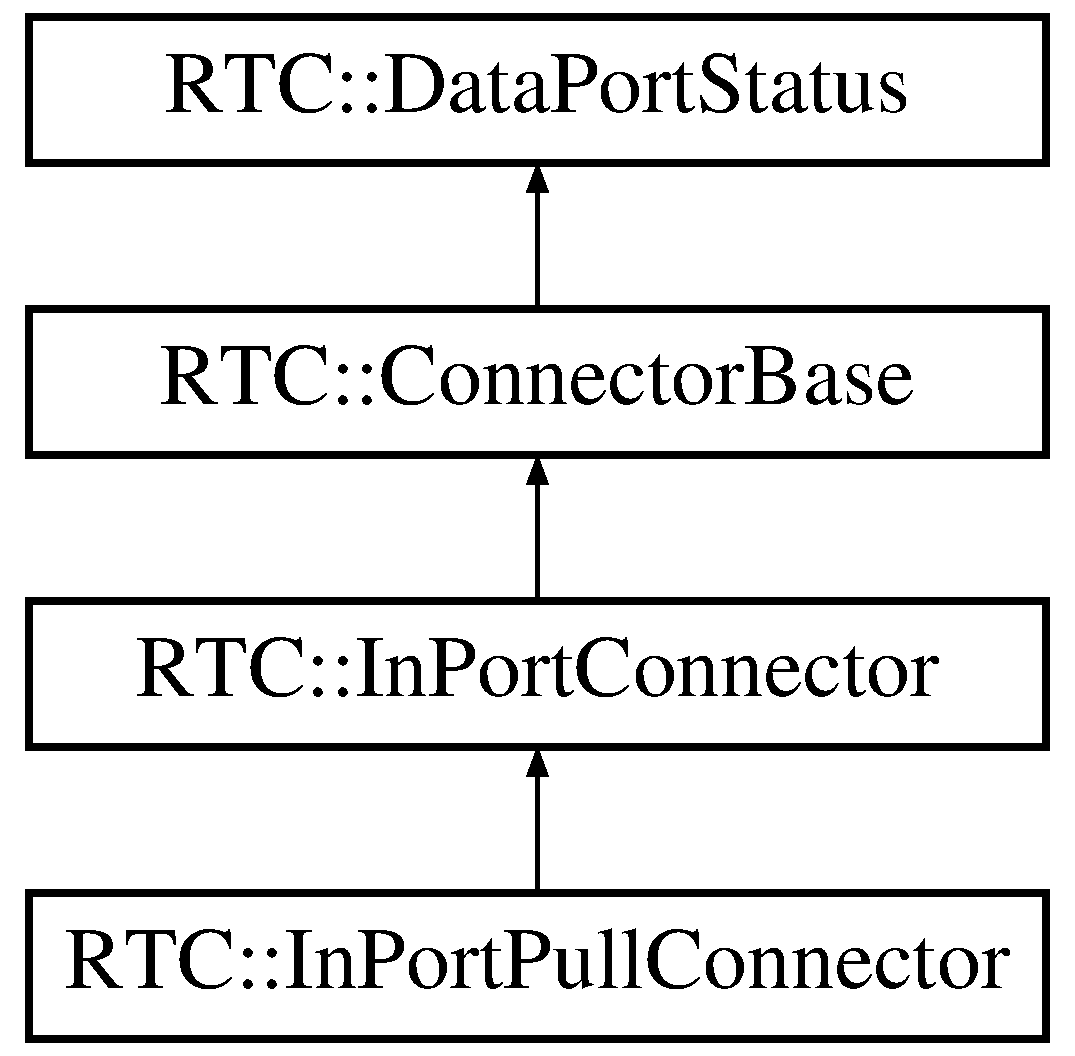
\includegraphics[height=4cm]{classRTC_1_1InPortPullConnector}
\end{center}
\end{figure}
\subsection*{Public Member Functions}
\begin{DoxyCompactItemize}
\item 
DATAPORTSTATUS\_\-ENUM {\bf InPortPullConnector} ({\bf ConnectorInfo} info, {\bf OutPortConsumer} $\ast$consumer, {\bf ConnectorListeners} \&listeners, {\bf CdrBufferBase} $\ast$buffer=0)
\begin{DoxyCompactList}\small\item\em Constructor. \item\end{DoxyCompactList}\item 
virtual {\bf $\sim$InPortPullConnector} ()
\begin{DoxyCompactList}\small\item\em Destructor. \item\end{DoxyCompactList}\item 
virtual ReturnCode {\bf read} (cdrMemoryStream \&data)
\begin{DoxyCompactList}\small\item\em Destructor. \item\end{DoxyCompactList}\item 
virtual ReturnCode {\bf disconnect} ()
\begin{DoxyCompactList}\small\item\em Disconnect connection. \item\end{DoxyCompactList}\item 
virtual void {\bf activate} ()
\begin{DoxyCompactList}\small\item\em Connector activation. \item\end{DoxyCompactList}\item 
virtual void {\bf deactivate} ()
\begin{DoxyCompactList}\small\item\em Connector deactivation. \item\end{DoxyCompactList}\end{DoxyCompactItemize}
\subsection*{Protected Member Functions}
\begin{DoxyCompactItemize}
\item 
{\bf CdrBufferBase} $\ast$ {\bf createBuffer} ({\bf ConnectorInfo} \&info)
\begin{DoxyCompactList}\small\item\em create buffer \item\end{DoxyCompactList}\item 
void {\bf onConnect} ()
\begin{DoxyCompactList}\small\item\em Invoke callback when connection is established. \item\end{DoxyCompactList}\item 
void {\bf onDisconnect} ()
\begin{DoxyCompactList}\small\item\em Invoke callback when connection is destroied. \item\end{DoxyCompactList}\end{DoxyCompactItemize}


\subsection{Detailed Description}
\doxyref{InPortPullConnector}{p.}{classRTC_1_1InPortPullConnector} class. Connector class of \doxyref{InPort}{p.}{classRTC_1_1InPort} for pull type dataflow. When \char`\"{}pull\char`\"{} is specified as dataflow\_\-type at the time of establishing connection, this object is generated and owned by the \doxyref{InPort}{p.}{classRTC_1_1InPort}. This connector and \doxyref{InPortPullConnector}{p.}{classRTC_1_1InPortPullConnector} make a pair and realize pull type dataflow of data ports. One connector corresponds to one connection which provides a data stream. Connector is distinguished by ID of the UUID that is generated at establishing connection.

\doxyref{InPortPullConnector}{p.}{classRTC_1_1InPortPullConnector} owns and manages the following objects.


\begin{DoxyItemize}
\item \doxyref{InPortConsumer}{p.}{classRTC_1_1InPortConsumer}
\item Buffer
\end{DoxyItemize}

Data written into the \doxyref{OutPort}{p.}{classRTC_1_1OutPort} is passed to the \doxyref{OutPortPullConnector::write()}{p.}{classRTC_1_1OutPortPullConnector_a9fbb676086061d99ce808818b6ddc316}, and is written into the buffer. Consequently, \doxyref{InPort::read()}{p.}{classRTC_1_1InPort_a1b6e58e0c821b46148266ddfd0b9bd54} and \doxyref{InPortPullConnector::read()}{p.}{classRTC_1_1InPortPullConnector_ac2bfcf970c6c0422e279af7d3b638efd} call \doxyref{OutPortConsumer::get()}{p.}{classRTC_1_1OutPortConsumer_acd8302e6ded9e796afb047aff0bc1c0e}, and it reads data from the buffer of \doxyref{OutPortPullConnector}{p.}{classRTC_1_1OutPortPullConnector}. Finally data would be written into the InPortPullConnector's buffer.

\begin{DoxySince}{Since}
1.0.0 
\end{DoxySince}


\subsection{Constructor \& Destructor Documentation}
\index{RTC::InPortPullConnector@{RTC::InPortPullConnector}!InPortPullConnector@{InPortPullConnector}}
\index{InPortPullConnector@{InPortPullConnector}!RTC::InPortPullConnector@{RTC::InPortPullConnector}}
\subsubsection[{InPortPullConnector}]{\setlength{\rightskip}{0pt plus 5cm}DATAPORTSTATUS\_\-ENUM RTC::InPortPullConnector::InPortPullConnector ({\bf ConnectorInfo} {\em info}, \/  {\bf OutPortConsumer} $\ast$ {\em consumer}, \/  {\bf ConnectorListeners} \& {\em listeners}, \/  {\bf CdrBufferBase} $\ast$ {\em buffer} = {\ttfamily 0})}\label{classRTC_1_1InPortPullConnector_af6b3d5b96862a4569ff3d25a24d591d6}


Constructor. 

InPortPullConnector's constructor is given the following arguments. According to \doxyref{ConnectorInfo}{p.}{classRTC_1_1ConnectorInfo} which includes connection information, a buffer is created. It is also given a pointer to the consumer object for the \doxyref{OutPort}{p.}{classRTC_1_1OutPort} interface. The owner-\/ship of the pointer is owned by this \doxyref{OutPortPullConnector}{p.}{classRTC_1_1OutPortPullConnector}, it has responsibility to destruct the \doxyref{OutPortConsumer}{p.}{classRTC_1_1OutPortConsumer}. \doxyref{OutPortPullConnector}{p.}{classRTC_1_1OutPortPullConnector} also has \doxyref{ConnectorListeners}{p.}{classRTC_1_1ConnectorListeners} to provide event callback mechanisms, and they would be called at the proper timing. If data buffer is given by \doxyref{OutPortBase}{p.}{classRTC_1_1OutPortBase}, the pointer to the buffer is also given as arguments.


\begin{DoxyParams}{Parameters}
\item[{\em info}]\doxyref{ConnectorInfo}{p.}{classRTC_1_1ConnectorInfo} \item[{\em consumer}]\doxyref{OutPortConsumer}{p.}{classRTC_1_1OutPortConsumer} \item[{\em listeners}]\doxyref{ConnectorListeners}{p.}{classRTC_1_1ConnectorListeners} type lsitener object list \item[{\em buffer}]CdrBufferBase type buffer \end{DoxyParams}
\index{RTC::InPortPullConnector@{RTC::InPortPullConnector}!$\sim$InPortPullConnector@{$\sim$InPortPullConnector}}
\index{$\sim$InPortPullConnector@{$\sim$InPortPullConnector}!RTC::InPortPullConnector@{RTC::InPortPullConnector}}
\subsubsection[{$\sim$InPortPullConnector}]{\setlength{\rightskip}{0pt plus 5cm}virtual RTC::InPortPullConnector::$\sim$InPortPullConnector ()\hspace{0.3cm}{\ttfamily  [virtual]}}\label{classRTC_1_1InPortPullConnector_abfc40c54105ad4cce78489b97ad91620}


Destructor. 

This operation calls \doxyref{disconnect()}{p.}{classRTC_1_1InPortPullConnector_a74e8c2fbfdbbacd1d3a67b4017b993df}, which destructs and deletes the consumer, the publisher and the buffer. 

\subsection{Member Function Documentation}
\index{RTC::InPortPullConnector@{RTC::InPortPullConnector}!activate@{activate}}
\index{activate@{activate}!RTC::InPortPullConnector@{RTC::InPortPullConnector}}
\subsubsection[{activate}]{\setlength{\rightskip}{0pt plus 5cm}virtual void RTC::InPortPullConnector::activate ()\hspace{0.3cm}{\ttfamily  [inline, virtual]}}\label{classRTC_1_1InPortPullConnector_a0caf7d4d08dec18fd2973b39d2bc497d}


Connector activation. 

This operation activates this connector 

Implements {\bf RTC::ConnectorBase} \doxyref{}{p.}{classRTC_1_1ConnectorBase_a6f7f9ddd882546044f911d66aefee665}.

\index{RTC::InPortPullConnector@{RTC::InPortPullConnector}!createBuffer@{createBuffer}}
\index{createBuffer@{createBuffer}!RTC::InPortPullConnector@{RTC::InPortPullConnector}}
\subsubsection[{createBuffer}]{\setlength{\rightskip}{0pt plus 5cm}{\bf CdrBufferBase}$\ast$ RTC::InPortPullConnector::createBuffer ({\bf ConnectorInfo} \& {\em info})\hspace{0.3cm}{\ttfamily  [protected]}}\label{classRTC_1_1InPortPullConnector_a92a27d869ccda93ba355c55b8a99172c}


create buffer 

This function creates a buffer based on given information.


\begin{DoxyParams}{Parameters}
\item[{\em info}]Connector information \end{DoxyParams}
\begin{DoxyReturn}{Returns}
The poitner to the buffer 
\end{DoxyReturn}
\index{RTC::InPortPullConnector@{RTC::InPortPullConnector}!deactivate@{deactivate}}
\index{deactivate@{deactivate}!RTC::InPortPullConnector@{RTC::InPortPullConnector}}
\subsubsection[{deactivate}]{\setlength{\rightskip}{0pt plus 5cm}virtual void RTC::InPortPullConnector::deactivate ()\hspace{0.3cm}{\ttfamily  [inline, virtual]}}\label{classRTC_1_1InPortPullConnector_a1dcb7d9c9c4eb8e4667180f1da142788}


Connector deactivation. 

This operation deactivates this connector 

Implements {\bf RTC::ConnectorBase} \doxyref{}{p.}{classRTC_1_1ConnectorBase_a8fe6a1bfe8d5ee586d51293b2bcf36d1}.

\index{RTC::InPortPullConnector@{RTC::InPortPullConnector}!disconnect@{disconnect}}
\index{disconnect@{disconnect}!RTC::InPortPullConnector@{RTC::InPortPullConnector}}
\subsubsection[{disconnect}]{\setlength{\rightskip}{0pt plus 5cm}virtual ReturnCode RTC::InPortPullConnector::disconnect ()\hspace{0.3cm}{\ttfamily  [virtual]}}\label{classRTC_1_1InPortPullConnector_a74e8c2fbfdbbacd1d3a67b4017b993df}


Disconnect connection. 

This operation disconnect this connection 

Implements {\bf RTC::InPortConnector} \doxyref{}{p.}{classRTC_1_1InPortConnector_a8677105bbf5ae5ed3e79dc3b057ea0b9}.

\index{RTC::InPortPullConnector@{RTC::InPortPullConnector}!onConnect@{onConnect}}
\index{onConnect@{onConnect}!RTC::InPortPullConnector@{RTC::InPortPullConnector}}
\subsubsection[{onConnect}]{\setlength{\rightskip}{0pt plus 5cm}void RTC::InPortPullConnector::onConnect ()\hspace{0.3cm}{\ttfamily  [protected]}}\label{classRTC_1_1InPortPullConnector_af1d4497434d7a0dbc8be49d92b163ad7}


Invoke callback when connection is established. 

\index{RTC::InPortPullConnector@{RTC::InPortPullConnector}!onDisconnect@{onDisconnect}}
\index{onDisconnect@{onDisconnect}!RTC::InPortPullConnector@{RTC::InPortPullConnector}}
\subsubsection[{onDisconnect}]{\setlength{\rightskip}{0pt plus 5cm}void RTC::InPortPullConnector::onDisconnect ()\hspace{0.3cm}{\ttfamily  [protected]}}\label{classRTC_1_1InPortPullConnector_a81a833e06ac3ea9a690825b404c48b3a}


Invoke callback when connection is destroied. 

\index{RTC::InPortPullConnector@{RTC::InPortPullConnector}!read@{read}}
\index{read@{read}!RTC::InPortPullConnector@{RTC::InPortPullConnector}}
\subsubsection[{read}]{\setlength{\rightskip}{0pt plus 5cm}virtual ReturnCode RTC::InPortPullConnector::read (cdrMemoryStream \& {\em data})\hspace{0.3cm}{\ttfamily  [virtual]}}\label{classRTC_1_1InPortPullConnector_ac2bfcf970c6c0422e279af7d3b638efd}


Destructor. 

This function get data from \doxyref{OutPortConsumer}{p.}{classRTC_1_1OutPortConsumer}. If data is read properly, this function will return PORT\_\-OK return code. Except normal return, BUFFER\_\-EMPTY, TIMEOUT, PRECONDITION\_\-NOT\_\-MET and PORT\_\-ERROR will be returned as error codes.

\begin{DoxyReturn}{Returns}
PORT\_\-OK Normal return BUFFER\_\-EMPTY Buffer empty TIMEOUT Timeout PRECONDITION\_\-NOT\_\-MET Preconditin not met PORT\_\-ERROR Other error 
\end{DoxyReturn}


Implements {\bf RTC::InPortConnector} \doxyref{}{p.}{classRTC_1_1InPortConnector_a2ffc997f36cb6549029852484327bffd}.


\section{RTC::InPortPushConnector Class Reference}
\label{classRTC_1_1InPortPushConnector}\index{RTC::InPortPushConnector@{RTC::InPortPushConnector}}


\doxyref{InPortPushConnector}{p.}{classRTC_1_1InPortPushConnector} class.  




{\ttfamily \#include $<$InPortPushConnector.h$>$}

Inheritance diagram for RTC::InPortPushConnector:\begin{figure}[H]
\begin{center}
\leavevmode
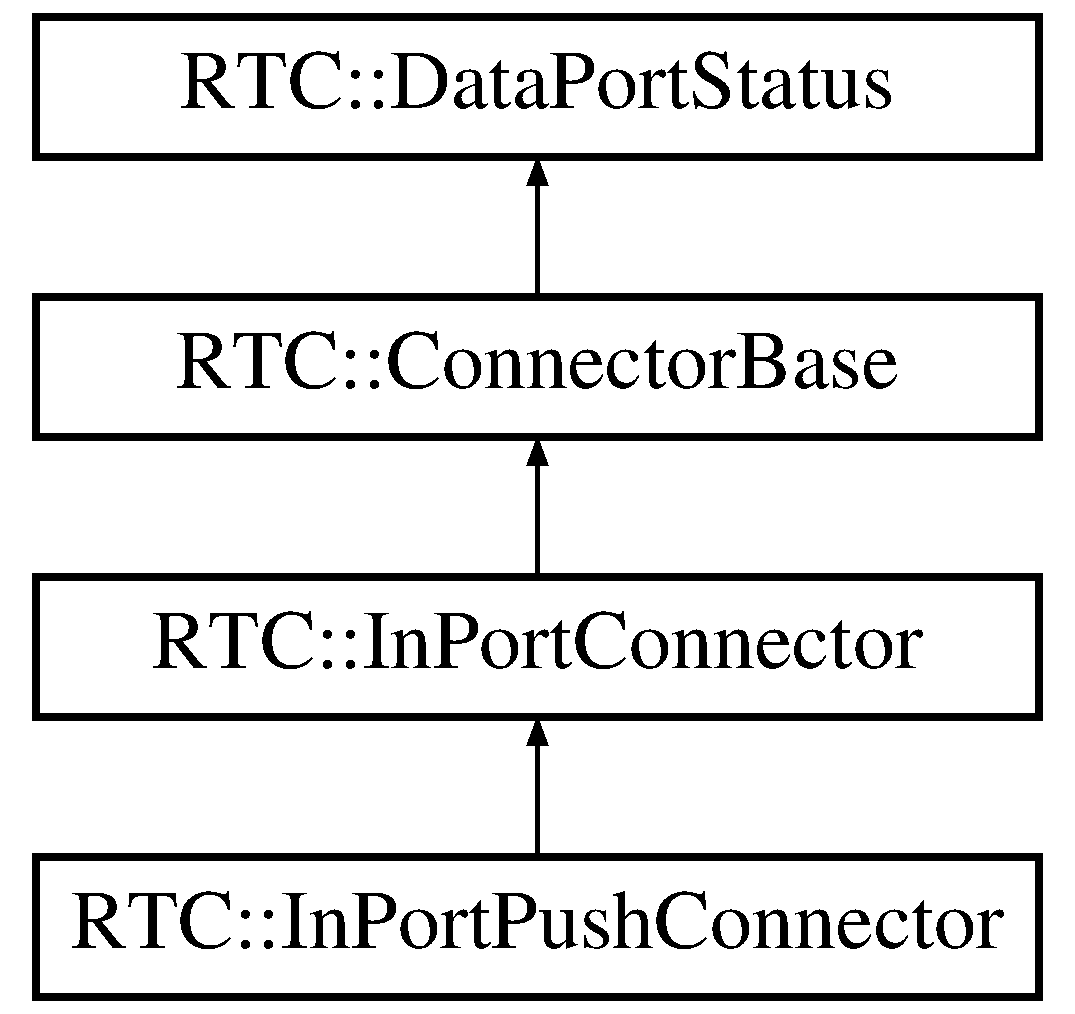
\includegraphics[height=4cm]{classRTC_1_1InPortPushConnector}
\end{center}
\end{figure}
\subsection*{Public Member Functions}
\begin{DoxyCompactItemize}
\item 
DATAPORTSTATUS\_\-ENUM {\bf InPortPushConnector} ({\bf ConnectorInfo} info, {\bf InPortProvider} $\ast$provider, {\bf ConnectorListeners} \&listeners, {\bf CdrBufferBase} $\ast$buffer=0)
\item 
virtual {\bf $\sim$InPortPushConnector} ()
\begin{DoxyCompactList}\small\item\em Destructor. \item\end{DoxyCompactList}\item 
virtual ReturnCode {\bf read} (cdrMemoryStream \&data)
\begin{DoxyCompactList}\small\item\em Reading data. \item\end{DoxyCompactList}\item 
virtual ReturnCode {\bf disconnect} ()
\begin{DoxyCompactList}\small\item\em disconnect \item\end{DoxyCompactList}\item 
virtual void {\bf activate} ()
\begin{DoxyCompactList}\small\item\em Connector activation. \item\end{DoxyCompactList}\item 
virtual void {\bf deactivate} ()
\begin{DoxyCompactList}\small\item\em Connector deactivation. \item\end{DoxyCompactList}\end{DoxyCompactItemize}
\subsection*{Protected Member Functions}
\begin{DoxyCompactItemize}
\item 
virtual {\bf CdrBufferBase} $\ast$ {\bf createBuffer} ({\bf ConnectorInfo} \&info)
\begin{DoxyCompactList}\small\item\em create buffer \item\end{DoxyCompactList}\item 
void {\bf onConnect} ()
\begin{DoxyCompactList}\small\item\em Invoke callback when connection is established. \item\end{DoxyCompactList}\item 
void {\bf onDisconnect} ()
\begin{DoxyCompactList}\small\item\em Invoke callback when connection is destroied. \item\end{DoxyCompactList}\end{DoxyCompactItemize}


\subsection{Detailed Description}
\doxyref{InPortPushConnector}{p.}{classRTC_1_1InPortPushConnector} class. Connector class of \doxyref{InPort}{p.}{classRTC_1_1InPort} for push type dataflow. When \char`\"{}push\char`\"{} is specified as dataflow\_\-type at the time of establishing connection, this object is generated and owned by the \doxyref{InPort}{p.}{classRTC_1_1InPort}. This connector and \doxyref{OutPortPushConnector}{p.}{classRTC_1_1OutPortPushConnector} make a pair and realize push type dataflow of data ports. One connector corresponds to one connection which provides a data stream. Connector is distinguished by ID of the UUID that is generated at establishing connection.

\doxyref{InPortPushConnector}{p.}{classRTC_1_1InPortPushConnector} owns and manages the following objects.


\begin{DoxyItemize}
\item \doxyref{OutPortConsumer}{p.}{classRTC_1_1OutPortConsumer}
\item Buffer
\end{DoxyItemize}

Data written into the \doxyref{OutPort}{p.}{classRTC_1_1OutPort} are passed to the InPortProvider::put() by \doxyref{OutPortConnector}{p.}{classRTC_1_1OutPortConnector}. The data is written into the buffer in the connector.

\begin{DoxySince}{Since}
1.0.0 
\end{DoxySince}


\subsection{Constructor \& Destructor Documentation}
\index{RTC::InPortPushConnector@{RTC::InPortPushConnector}!InPortPushConnector@{InPortPushConnector}}
\index{InPortPushConnector@{InPortPushConnector}!RTC::InPortPushConnector@{RTC::InPortPushConnector}}
\subsubsection[{InPortPushConnector}]{\setlength{\rightskip}{0pt plus 5cm}DATAPORTSTATUS\_\-ENUM RTC::InPortPushConnector::InPortPushConnector ({\bf ConnectorInfo} {\em info}, \/  {\bf InPortProvider} $\ast$ {\em provider}, \/  {\bf ConnectorListeners} \& {\em listeners}, \/  {\bf CdrBufferBase} $\ast$ {\em buffer} = {\ttfamily 0})}\label{classRTC_1_1InPortPushConnector_a3b84b5cb1d581592fe0839e62d1f1014}
\index{RTC::InPortPushConnector@{RTC::InPortPushConnector}!$\sim$InPortPushConnector@{$\sim$InPortPushConnector}}
\index{$\sim$InPortPushConnector@{$\sim$InPortPushConnector}!RTC::InPortPushConnector@{RTC::InPortPushConnector}}
\subsubsection[{$\sim$InPortPushConnector}]{\setlength{\rightskip}{0pt plus 5cm}virtual RTC::InPortPushConnector::$\sim$InPortPushConnector ()\hspace{0.3cm}{\ttfamily  [virtual]}}\label{classRTC_1_1InPortPushConnector_a8768a0ed4abe61057e65db0cfb48b31c}


Destructor. 

This operation calls \doxyref{disconnect()}{p.}{classRTC_1_1InPortPushConnector_afb5920eabaa874b43bc900348a2fb2ad}, which destructs and deletes the consumer, the publisher and the buffer. 

\subsection{Member Function Documentation}
\index{RTC::InPortPushConnector@{RTC::InPortPushConnector}!activate@{activate}}
\index{activate@{activate}!RTC::InPortPushConnector@{RTC::InPortPushConnector}}
\subsubsection[{activate}]{\setlength{\rightskip}{0pt plus 5cm}virtual void RTC::InPortPushConnector::activate ()\hspace{0.3cm}{\ttfamily  [inline, virtual]}}\label{classRTC_1_1InPortPushConnector_a5a34568fa4c67ad895e7842882077e30}


Connector activation. 

This operation activates this connector 

Implements {\bf RTC::ConnectorBase} \doxyref{}{p.}{classRTC_1_1ConnectorBase_a6f7f9ddd882546044f911d66aefee665}.

\index{RTC::InPortPushConnector@{RTC::InPortPushConnector}!createBuffer@{createBuffer}}
\index{createBuffer@{createBuffer}!RTC::InPortPushConnector@{RTC::InPortPushConnector}}
\subsubsection[{createBuffer}]{\setlength{\rightskip}{0pt plus 5cm}virtual {\bf CdrBufferBase}$\ast$ RTC::InPortPushConnector::createBuffer ({\bf ConnectorInfo} \& {\em info})\hspace{0.3cm}{\ttfamily  [protected, virtual]}}\label{classRTC_1_1InPortPushConnector_abe343b1be5c354ec3f6b0385755a34e2}


create buffer 

This function creates a buffer based on given information.


\begin{DoxyParams}{Parameters}
\item[{\em info}]Connector information \end{DoxyParams}
\begin{DoxyReturn}{Returns}
The poitner to the buffer 
\end{DoxyReturn}
\index{RTC::InPortPushConnector@{RTC::InPortPushConnector}!deactivate@{deactivate}}
\index{deactivate@{deactivate}!RTC::InPortPushConnector@{RTC::InPortPushConnector}}
\subsubsection[{deactivate}]{\setlength{\rightskip}{0pt plus 5cm}virtual void RTC::InPortPushConnector::deactivate ()\hspace{0.3cm}{\ttfamily  [inline, virtual]}}\label{classRTC_1_1InPortPushConnector_af93f9456bc93eba17fda8b2f0ceda313}


Connector deactivation. 

This operation deactivates this connector 

Implements {\bf RTC::ConnectorBase} \doxyref{}{p.}{classRTC_1_1ConnectorBase_a8fe6a1bfe8d5ee586d51293b2bcf36d1}.

\index{RTC::InPortPushConnector@{RTC::InPortPushConnector}!disconnect@{disconnect}}
\index{disconnect@{disconnect}!RTC::InPortPushConnector@{RTC::InPortPushConnector}}
\subsubsection[{disconnect}]{\setlength{\rightskip}{0pt plus 5cm}virtual ReturnCode RTC::InPortPushConnector::disconnect ()\hspace{0.3cm}{\ttfamily  [virtual]}}\label{classRTC_1_1InPortPushConnector_afb5920eabaa874b43bc900348a2fb2ad}


disconnect 

This operation destruct and delete the consumer, the publisher and the buffer.

\begin{DoxyReturn}{Returns}
PORT\_\-OK 
\end{DoxyReturn}


Implements {\bf RTC::InPortConnector} \doxyref{}{p.}{classRTC_1_1InPortConnector_a8677105bbf5ae5ed3e79dc3b057ea0b9}.

\index{RTC::InPortPushConnector@{RTC::InPortPushConnector}!onConnect@{onConnect}}
\index{onConnect@{onConnect}!RTC::InPortPushConnector@{RTC::InPortPushConnector}}
\subsubsection[{onConnect}]{\setlength{\rightskip}{0pt plus 5cm}void RTC::InPortPushConnector::onConnect ()\hspace{0.3cm}{\ttfamily  [protected]}}\label{classRTC_1_1InPortPushConnector_adb41bf605ce4ff42b8c841f37130932f}


Invoke callback when connection is established. 

\index{RTC::InPortPushConnector@{RTC::InPortPushConnector}!onDisconnect@{onDisconnect}}
\index{onDisconnect@{onDisconnect}!RTC::InPortPushConnector@{RTC::InPortPushConnector}}
\subsubsection[{onDisconnect}]{\setlength{\rightskip}{0pt plus 5cm}void RTC::InPortPushConnector::onDisconnect ()\hspace{0.3cm}{\ttfamily  [protected]}}\label{classRTC_1_1InPortPushConnector_a99a1d5d8ab314f298f41e1a43f6c81fb}


Invoke callback when connection is destroied. 

\index{RTC::InPortPushConnector@{RTC::InPortPushConnector}!read@{read}}
\index{read@{read}!RTC::InPortPushConnector@{RTC::InPortPushConnector}}
\subsubsection[{read}]{\setlength{\rightskip}{0pt plus 5cm}virtual ReturnCode RTC::InPortPushConnector::read (cdrMemoryStream \& {\em data})\hspace{0.3cm}{\ttfamily  [virtual]}}\label{classRTC_1_1InPortPushConnector_a1403a79f0e0ce7d6c34b4385db6ed8ef}


Reading data. 

This function reads data from the buffer. If data is read properly, this function will return PORT\_\-OK return code. Except normal return, BUFFER\_\-EMPTY, TIMEOUT, PRECONDITION\_\-NOT\_\-MET and PORT\_\-ERROR will be returned as error codes.

\begin{DoxyReturn}{Returns}
PORT\_\-OK Normal return BUFFER\_\-EMPTY Buffer empty TIMEOUT Timeout PRECONDITION\_\-NOT\_\-MET Preconditin not met PORT\_\-ERROR Other error 
\end{DoxyReturn}


Implements {\bf RTC::InPortConnector} \doxyref{}{p.}{classRTC_1_1InPortConnector_a2ffc997f36cb6549029852484327bffd}.


\section{RTC::Manager::InstanceName Struct Reference}
\label{structRTC_1_1Manager_1_1InstanceName}\index{RTC::Manager::InstanceName@{RTC::Manager::InstanceName}}


{\ttfamily \#include $<$Manager.h$>$}

\subsection*{Public Member Functions}
\begin{DoxyCompactItemize}
\item 
{\bf InstanceName} ({\bf RTObject\_\-impl} $\ast$comp)
\item 
{\bf InstanceName} (const char $\ast$name)
\item 
{\bf InstanceName} (const std::string name)
\item 
bool {\bf operator()} ({\bf RTObject\_\-impl} $\ast$comp)
\end{DoxyCompactItemize}
\subsection*{Public Attributes}
\begin{DoxyCompactItemize}
\item 
std::string {\bf m\_\-name}
\end{DoxyCompactItemize}


\subsection{Constructor \& Destructor Documentation}
\index{RTC::Manager::InstanceName@{RTC::Manager::InstanceName}!InstanceName@{InstanceName}}
\index{InstanceName@{InstanceName}!RTC::Manager::InstanceName@{RTC::Manager::InstanceName}}
\subsubsection[{InstanceName}]{\setlength{\rightskip}{0pt plus 5cm}RTC::Manager::InstanceName::InstanceName ({\bf RTObject\_\-impl} $\ast$ {\em comp})}\label{structRTC_1_1Manager_1_1InstanceName_a79521954523289d88f986d78abf73939}
\index{RTC::Manager::InstanceName@{RTC::Manager::InstanceName}!InstanceName@{InstanceName}}
\index{InstanceName@{InstanceName}!RTC::Manager::InstanceName@{RTC::Manager::InstanceName}}
\subsubsection[{InstanceName}]{\setlength{\rightskip}{0pt plus 5cm}RTC::Manager::InstanceName::InstanceName (const char $\ast$ {\em name})}\label{structRTC_1_1Manager_1_1InstanceName_a7317d4881eff0b19d18f918c2252ba44}
\index{RTC::Manager::InstanceName@{RTC::Manager::InstanceName}!InstanceName@{InstanceName}}
\index{InstanceName@{InstanceName}!RTC::Manager::InstanceName@{RTC::Manager::InstanceName}}
\subsubsection[{InstanceName}]{\setlength{\rightskip}{0pt plus 5cm}RTC::Manager::InstanceName::InstanceName (const std::string {\em name})}\label{structRTC_1_1Manager_1_1InstanceName_aeaccb5c948903147fec54a30244aeeab}


\subsection{Member Function Documentation}
\index{RTC::Manager::InstanceName@{RTC::Manager::InstanceName}!operator()@{operator()}}
\index{operator()@{operator()}!RTC::Manager::InstanceName@{RTC::Manager::InstanceName}}
\subsubsection[{operator()}]{\setlength{\rightskip}{0pt plus 5cm}bool RTC::Manager::InstanceName::operator() ({\bf RTObject\_\-impl} $\ast$ {\em comp})}\label{structRTC_1_1Manager_1_1InstanceName_aea1ede840c201f3e9afd68385e4b9a9d}


\subsection{Member Data Documentation}
\index{RTC::Manager::InstanceName@{RTC::Manager::InstanceName}!m\_\-name@{m\_\-name}}
\index{m\_\-name@{m\_\-name}!RTC::Manager::InstanceName@{RTC::Manager::InstanceName}}
\subsubsection[{m\_\-name}]{\setlength{\rightskip}{0pt plus 5cm}std::string {\bf RTC::Manager::InstanceName::m\_\-name}}\label{structRTC_1_1Manager_1_1InstanceName_aa3744c310d19e37f9a793b0837f744b2}

\section{構造体 RTC::ModuleManager::InvalidArguments}
\label{structRTC_1_1ModuleManager_1_1InvalidArguments}\index{RTC::ModuleManager::InvalidArguments@{RTC::ModuleManager::InvalidArguments}}


指定引数不正時例外処理用構造体  




{\ttfamily \#include $<$ModuleManager.h$>$}

RTC::ModuleManager::InvalidArgumentsに対する継承グラフ\begin{figure}[H]
\begin{center}
\leavevmode
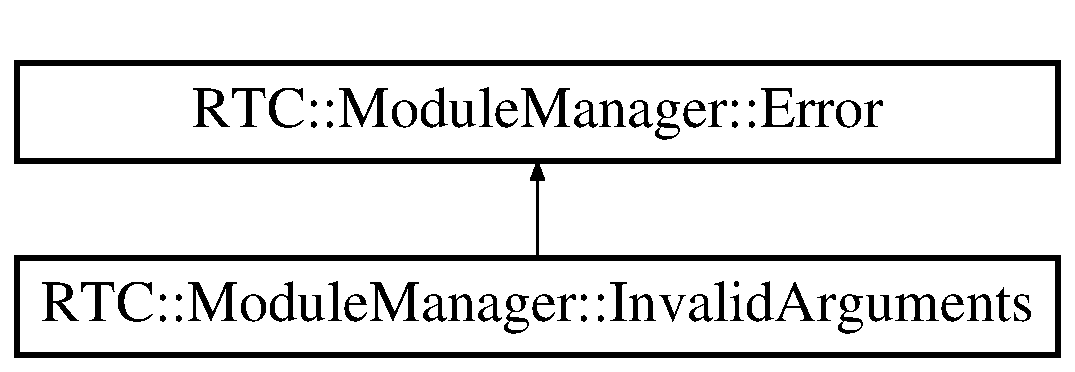
\includegraphics[height=2cm]{structRTC_1_1ModuleManager_1_1InvalidArguments}
\end{center}
\end{figure}
\subsection*{Public メソッド}
\begin{DoxyCompactItemize}
\item 
{\bf InvalidArguments} (const std::string \&\_\-reason)
\end{DoxyCompactItemize}


\subsection{説明}
指定引数不正時例外処理用構造体 

\subsection{コンストラクタとデストラクタ}
\index{RTC::ModuleManager::InvalidArguments@{RTC::ModuleManager::InvalidArguments}!InvalidArguments@{InvalidArguments}}
\index{InvalidArguments@{InvalidArguments}!RTC::ModuleManager::InvalidArguments@{RTC::ModuleManager::InvalidArguments}}
\subsubsection[{InvalidArguments}]{\setlength{\rightskip}{0pt plus 5cm}RTC::ModuleManager::InvalidArguments::InvalidArguments (const std::string \& {\em \_\-reason})\hspace{0.3cm}{\ttfamily  [inline]}}\label{structRTC_1_1ModuleManager_1_1InvalidArguments_a4fc5572f3222647ebebc44121c7236ed}

\section{RTC::ModuleManager::InvalidOperation Struct Reference}
\label{structRTC_1_1ModuleManager_1_1InvalidOperation}\index{RTC::ModuleManager::InvalidOperation@{RTC::ModuleManager::InvalidOperation}}


Structure for exception handling when specified operation is invalid.  




{\ttfamily \#include $<$ModuleManager.h$>$}

Inheritance diagram for RTC::ModuleManager::InvalidOperation:\begin{figure}[H]
\begin{center}
\leavevmode
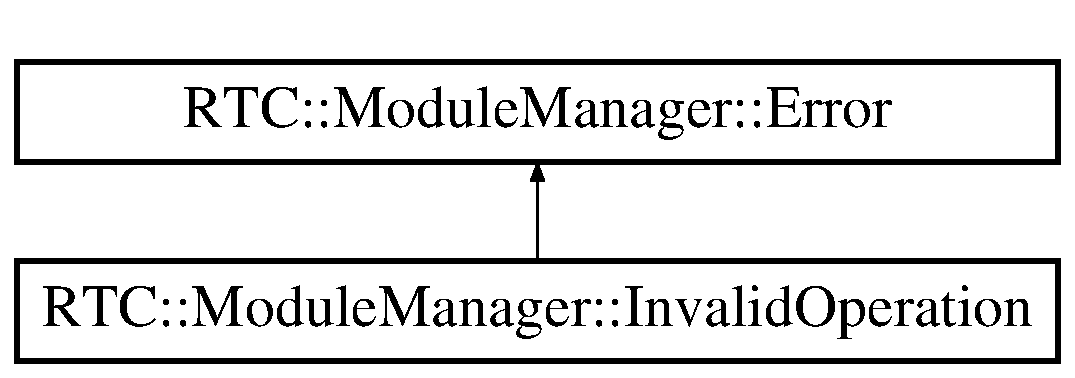
\includegraphics[height=2cm]{structRTC_1_1ModuleManager_1_1InvalidOperation}
\end{center}
\end{figure}
\subsection*{Public Member Functions}
\begin{DoxyCompactItemize}
\item 
{\bf InvalidOperation} (const std::string \&\_\-reason)
\end{DoxyCompactItemize}


\subsection{Detailed Description}
Structure for exception handling when specified operation is invalid. 

\subsection{Constructor \& Destructor Documentation}
\index{RTC::ModuleManager::InvalidOperation@{RTC::ModuleManager::InvalidOperation}!InvalidOperation@{InvalidOperation}}
\index{InvalidOperation@{InvalidOperation}!RTC::ModuleManager::InvalidOperation@{RTC::ModuleManager::InvalidOperation}}
\subsubsection[{InvalidOperation}]{\setlength{\rightskip}{0pt plus 5cm}RTC::ModuleManager::InvalidOperation::InvalidOperation (const std::string \& {\em \_\-reason})\hspace{0.3cm}{\ttfamily  [inline]}}\label{structRTC_1_1ModuleManager_1_1InvalidOperation_a49b14ed508206f3f05a14bcc5811de4a}

\section{RTC::PeriodicExecutionContext::invoke\_\-on\_\-rate\_\-changed Struct Reference}
\label{structRTC_1_1PeriodicExecutionContext_1_1invoke__on__rate__changed}\index{RTC::PeriodicExecutionContext::invoke\_\-on\_\-rate\_\-changed@{RTC::PeriodicExecutionContext::invoke\_\-on\_\-rate\_\-changed}}


Functor to invoke on\_\-rate\_\-changed.  




{\ttfamily \#include $<$PeriodicExecutionContext.h$>$}

\subsection*{Public Member Functions}
\begin{DoxyCompactItemize}
\item 
void {\bf operator()} ({\bf Comp} \&comp)
\end{DoxyCompactItemize}


\subsection{Detailed Description}
Functor to invoke on\_\-rate\_\-changed. 

\subsection{Member Function Documentation}
\index{RTC::PeriodicExecutionContext::invoke\_\-on\_\-rate\_\-changed@{RTC::PeriodicExecutionContext::invoke\_\-on\_\-rate\_\-changed}!operator()@{operator()}}
\index{operator()@{operator()}!RTC::PeriodicExecutionContext::invoke_on_rate_changed@{RTC::PeriodicExecutionContext::invoke\_\-on\_\-rate\_\-changed}}
\subsubsection[{operator()}]{\setlength{\rightskip}{0pt plus 5cm}void RTC::PeriodicExecutionContext::invoke\_\-on\_\-rate\_\-changed::operator() ({\bf Comp} \& {\em comp})\hspace{0.3cm}{\ttfamily  [inline]}}\label{structRTC_1_1PeriodicExecutionContext_1_1invoke__on__rate__changed_a374c72b2f2d5fa61d9eb6e3476731959}


References RTC::PeriodicExecutionContext::Comp::\_\-sm, and RTC::PeriodicExecutionContext::DFP$<$ Object $>$::on\_\-rate\_\-changed().


\section{RTC::PeriodicExecutionContext::invoke\_\-on\_\-shutdown Struct Reference}
\label{structRTC_1_1PeriodicExecutionContext_1_1invoke__on__shutdown}\index{RTC::PeriodicExecutionContext::invoke\_\-on\_\-shutdown@{RTC::PeriodicExecutionContext::invoke\_\-on\_\-shutdown}}


Functor to invoke on\_\-shutdown.  




{\ttfamily \#include $<$PeriodicExecutionContext.h$>$}

\subsection*{Public Member Functions}
\begin{DoxyCompactItemize}
\item 
void {\bf operator()} ({\bf Comp} \&comp)
\end{DoxyCompactItemize}


\subsection{Detailed Description}
Functor to invoke on\_\-shutdown. 

\subsection{Member Function Documentation}
\index{RTC::PeriodicExecutionContext::invoke\_\-on\_\-shutdown@{RTC::PeriodicExecutionContext::invoke\_\-on\_\-shutdown}!operator()@{operator()}}
\index{operator()@{operator()}!RTC::PeriodicExecutionContext::invoke_on_shutdown@{RTC::PeriodicExecutionContext::invoke\_\-on\_\-shutdown}}
\subsubsection[{operator()}]{\setlength{\rightskip}{0pt plus 5cm}void RTC::PeriodicExecutionContext::invoke\_\-on\_\-shutdown::operator() ({\bf Comp} \& {\em comp})\hspace{0.3cm}{\ttfamily  [inline]}}\label{structRTC_1_1PeriodicExecutionContext_1_1invoke__on__shutdown_a4da104c45a5f714bcfe37ec50055305a}


References RTC::PeriodicExecutionContext::Comp::\_\-sm, and RTC::PeriodicExecutionContext::DFP$<$ Object $>$::on\_\-shutdown().


\section{RTC::PeriodicExecutionContext::invoke\_\-on\_\-startup Struct Reference}
\label{structRTC_1_1PeriodicExecutionContext_1_1invoke__on__startup}\index{RTC::PeriodicExecutionContext::invoke\_\-on\_\-startup@{RTC::PeriodicExecutionContext::invoke\_\-on\_\-startup}}


Functor to invoke on\_\-startup.  




{\ttfamily \#include $<$PeriodicExecutionContext.h$>$}

\subsection*{Public Member Functions}
\begin{DoxyCompactItemize}
\item 
void {\bf operator()} ({\bf Comp} \&comp)
\end{DoxyCompactItemize}


\subsection{Detailed Description}
Functor to invoke on\_\-startup. 

\subsection{Member Function Documentation}
\index{RTC::PeriodicExecutionContext::invoke\_\-on\_\-startup@{RTC::PeriodicExecutionContext::invoke\_\-on\_\-startup}!operator()@{operator()}}
\index{operator()@{operator()}!RTC::PeriodicExecutionContext::invoke_on_startup@{RTC::PeriodicExecutionContext::invoke\_\-on\_\-startup}}
\subsubsection[{operator()}]{\setlength{\rightskip}{0pt plus 5cm}void RTC::PeriodicExecutionContext::invoke\_\-on\_\-startup::operator() ({\bf Comp} \& {\em comp})\hspace{0.3cm}{\ttfamily  [inline]}}\label{structRTC_1_1PeriodicExecutionContext_1_1invoke__on__startup_adda237953995471a223c0ec6123205e1}


References RTC::PeriodicExecutionContext::Comp::\_\-sm, and RTC::PeriodicExecutionContext::DFP$<$ Object $>$::on\_\-startup().


\section{構造体 RTC::PeriodicExecutionContext::invoke\_\-worker}
\label{structRTC_1_1PeriodicExecutionContext_1_1invoke__worker}\index{RTC::PeriodicExecutionContext::invoke\_\-worker@{RTC::PeriodicExecutionContext::invoke\_\-worker}}


ワーカー実行用ファンクタ  




{\ttfamily \#include $<$PeriodicExecutionContext.h$>$}

\subsection*{Public メソッド}
\begin{DoxyCompactItemize}
\item 
void {\bf operator()} ({\bf Comp} \&comp)
\end{DoxyCompactItemize}


\subsection{説明}
ワーカー実行用ファンクタ 

\subsection{関数}
\index{RTC::PeriodicExecutionContext::invoke\_\-worker@{RTC::PeriodicExecutionContext::invoke\_\-worker}!operator()@{operator()}}
\index{operator()@{operator()}!RTC::PeriodicExecutionContext::invoke_worker@{RTC::PeriodicExecutionContext::invoke\_\-worker}}
\subsubsection[{operator()}]{\setlength{\rightskip}{0pt plus 5cm}void RTC::PeriodicExecutionContext::invoke\_\-worker::operator() ({\bf Comp} \& {\em comp})\hspace{0.3cm}{\ttfamily  [inline]}}\label{structRTC_1_1PeriodicExecutionContext_1_1invoke__worker_ab7b7faf3e55941e7829e36d1a86cc211}


参照先 RTC::PeriodicExecutionContext::Comp::\_\-sm, と RTC::PeriodicExecutionContext::DFPBase::worker().


\section{CORBA\_\-Util::is\_\-corba\_\-object$<$ T $>$ Struct Template Reference}
\label{structCORBA__Util_1_1is__corba__object}\index{CORBA\_\-Util::is\_\-corba\_\-object@{CORBA\_\-Util::is\_\-corba\_\-object}}


is corba object traits class  




{\ttfamily \#include $<$Typename.h$>$}

\subsection*{Static Public Attributes}
\begin{DoxyCompactItemize}
\item 
static const bool {\bf value} = {\bf has\_\-nil}$<$T$>$::{\bf value}
\end{DoxyCompactItemize}


\subsection{Detailed Description}
\subsubsection*{template$<$typename T$>$ struct CORBA\_\-Util::is\_\-corba\_\-object$<$ T $>$}

is corba object traits class T is CORBA object -\/$>$ value = true T is not CORBA object -\/$>$ value = false 

\subsection{Member Data Documentation}
\index{CORBA\_\-Util::is\_\-corba\_\-object@{CORBA\_\-Util::is\_\-corba\_\-object}!value@{value}}
\index{value@{value}!CORBA_Util::is_corba_object@{CORBA\_\-Util::is\_\-corba\_\-object}}
\subsubsection[{value}]{\setlength{\rightskip}{0pt plus 5cm}template$<$typename T $>$ const bool {\bf CORBA\_\-Util::is\_\-corba\_\-object}$<$ T $>$::{\bf value} = {\bf has\_\-nil}$<$T$>$::{\bf value}\hspace{0.3cm}{\ttfamily  [static]}}\label{structCORBA__Util_1_1is__corba__object_a1ca9ab7460b29624bb71bf2a0b3e7a24}

\section{クラス ListenerBase}
\label{classListenerBase}\index{ListenerBase@{ListenerBase}}


\doxyref{ListenerBase}{p.}{classListenerBase} クラス.  




{\ttfamily \#include $<$Listener.h$>$}

ListenerBaseに対する継承グラフ\begin{figure}[H]
\begin{center}
\leavevmode
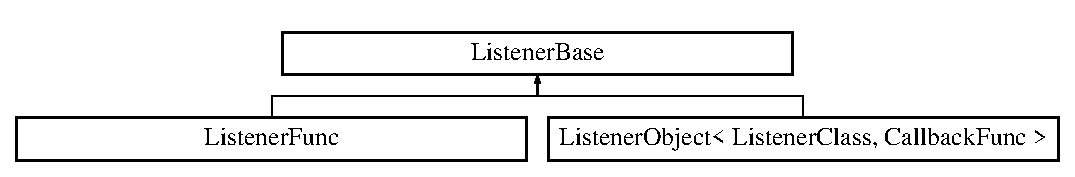
\includegraphics[height=1.93772cm]{classListenerBase}
\end{center}
\end{figure}
\subsection*{Public メソッド}
\begin{DoxyCompactItemize}
\item 
virtual {\bf $\sim$ListenerBase} ()
\item 
virtual void {\bf invoke} ()=0
\begin{DoxyCompactList}\small\item\em コールバック処理 \item\end{DoxyCompactList}\end{DoxyCompactItemize}


\subsection{説明}
\doxyref{ListenerBase}{p.}{classListenerBase} クラス. タイマーに登録するリスナー用抽象インターフェースクラス。

\begin{DoxySince}{から}
0.4.0 
\end{DoxySince}


\subsection{コンストラクタとデストラクタ}
\index{ListenerBase@{ListenerBase}!$\sim$ListenerBase@{$\sim$ListenerBase}}
\index{$\sim$ListenerBase@{$\sim$ListenerBase}!ListenerBase@{ListenerBase}}
\subsubsection[{$\sim$ListenerBase}]{\setlength{\rightskip}{0pt plus 5cm}virtual ListenerBase::$\sim$ListenerBase ()\hspace{0.3cm}{\ttfamily  [inline, virtual]}}\label{classListenerBase_ae9c4a6c29939edf6f10a3c0393fbf10d}
デストラクタ 

\subsection{関数}
\index{ListenerBase@{ListenerBase}!invoke@{invoke}}
\index{invoke@{invoke}!ListenerBase@{ListenerBase}}
\subsubsection[{invoke}]{\setlength{\rightskip}{0pt plus 5cm}virtual void ListenerBase::invoke ()\hspace{0.3cm}{\ttfamily  [pure virtual]}}\label{classListenerBase_af2cace07df880215fda280ed3cbe0b0b}


コールバック処理 

コールバック処理用純粋仮想関数 

{\bf ListenerObject$<$ ListenerClass, CallbackFunc $>$} \doxyref{}{p.}{classListenerObject_a89a5e9d005b8043419f4ccbb244f29d4}, と {\bf ListenerFunc} \doxyref{}{p.}{classListenerFunc_aaad57f69b0e6c85d9a6b01cec53bc74f}で実装されています。


\section{クラス ListenerFunc}
\label{classListenerFunc}\index{ListenerFunc@{ListenerFunc}}


\doxyref{ListenerFunc}{p.}{classListenerFunc} クラス.  




{\ttfamily \#include $<$Listener.h$>$}

ListenerFuncに対する継承グラフ\begin{figure}[H]
\begin{center}
\leavevmode
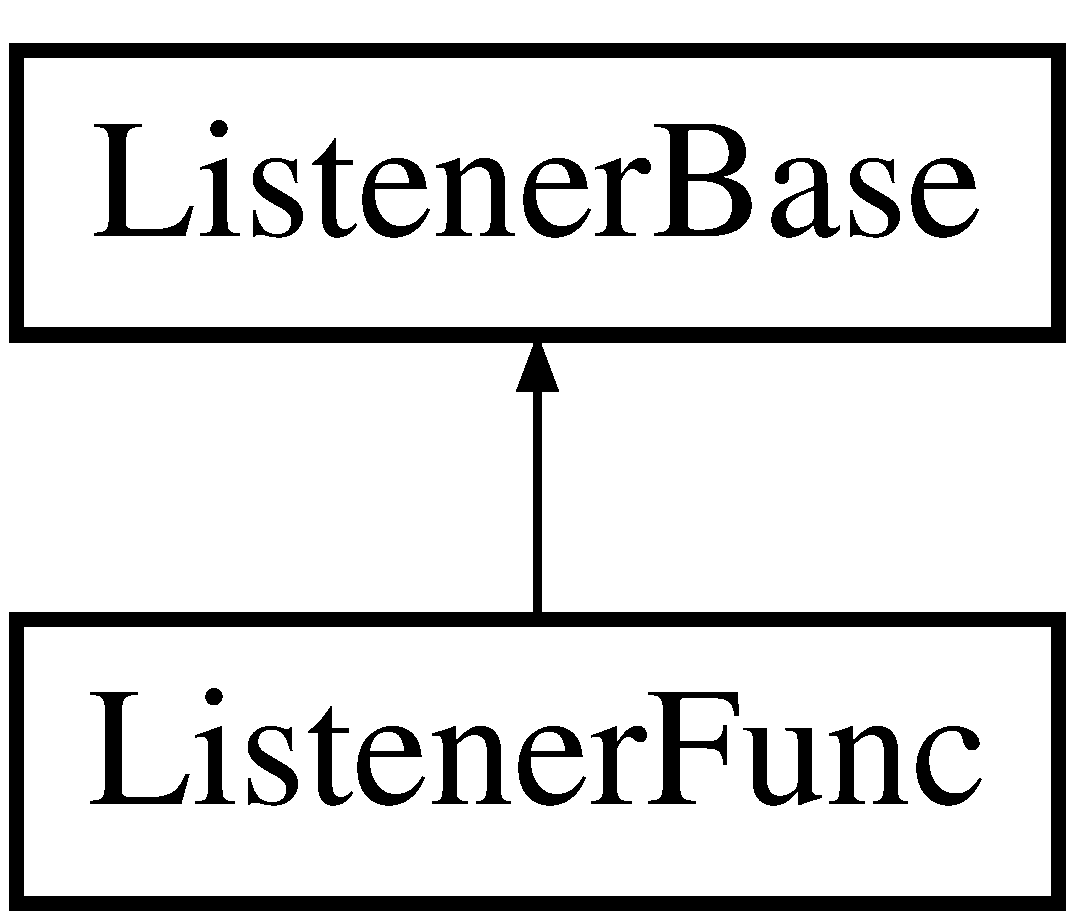
\includegraphics[height=2cm]{classListenerFunc}
\end{center}
\end{figure}
\subsection*{Public メソッド}
\begin{DoxyCompactItemize}
\item 
{\bf ListenerFunc} ({\bf CallbackFunc} cbf)
\begin{DoxyCompactList}\small\item\em コンストラクタ \item\end{DoxyCompactList}\item 
virtual {\bf $\sim$ListenerFunc} ()
\item 
virtual void {\bf invoke} ()
\begin{DoxyCompactList}\small\item\em コールバック処理 \item\end{DoxyCompactList}\end{DoxyCompactItemize}


\subsection{説明}
\doxyref{ListenerFunc}{p.}{classListenerFunc} クラス. コールバック用オブジェクト。

\begin{DoxySince}{から}
0.4.0 
\end{DoxySince}


\subsection{コンストラクタとデストラクタ}
\index{ListenerFunc@{ListenerFunc}!ListenerFunc@{ListenerFunc}}
\index{ListenerFunc@{ListenerFunc}!ListenerFunc@{ListenerFunc}}
\subsubsection[{ListenerFunc}]{\setlength{\rightskip}{0pt plus 5cm}ListenerFunc::ListenerFunc ({\bf CallbackFunc} {\em cbf})\hspace{0.3cm}{\ttfamily  [inline]}}\label{classListenerFunc_a5dbf54a5f4d18d7bd853e1a222a08e00}


コンストラクタ 

コンストラクタ


\begin{DoxyParams}{引数}
\item[{\em cbf}]コールバック用関数 \end{DoxyParams}
\index{ListenerFunc@{ListenerFunc}!$\sim$ListenerFunc@{$\sim$ListenerFunc}}
\index{$\sim$ListenerFunc@{$\sim$ListenerFunc}!ListenerFunc@{ListenerFunc}}
\subsubsection[{$\sim$ListenerFunc}]{\setlength{\rightskip}{0pt plus 5cm}virtual ListenerFunc::$\sim$ListenerFunc ()\hspace{0.3cm}{\ttfamily  [inline, virtual]}}\label{classListenerFunc_a6b6f2ac9f5899cccaefcadde69509ebf}
デストラクタ 

\subsection{関数}
\index{ListenerFunc@{ListenerFunc}!invoke@{invoke}}
\index{invoke@{invoke}!ListenerFunc@{ListenerFunc}}
\subsubsection[{invoke}]{\setlength{\rightskip}{0pt plus 5cm}virtual void ListenerFunc::invoke ()\hspace{0.3cm}{\ttfamily  [inline, virtual]}}\label{classListenerFunc_aaad57f69b0e6c85d9a6b01cec53bc74f}


コールバック処理 

コールバック処理用関数 

{\bf ListenerBase} \doxyref{}{p.}{classListenerBase_af2cace07df880215fda280ed3cbe0b0b}を実装しています。


\section{ListenerObject$<$ ListenerClass, CallbackFunc $>$ Class Template Reference}
\label{classListenerObject}\index{ListenerObject@{ListenerObject}}


\doxyref{ListenerObject}{p.}{classListenerObject} class.  




{\ttfamily \#include $<$Listener.h$>$}

Inheritance diagram for ListenerObject$<$ ListenerClass, CallbackFunc $>$:\begin{figure}[H]
\begin{center}
\leavevmode
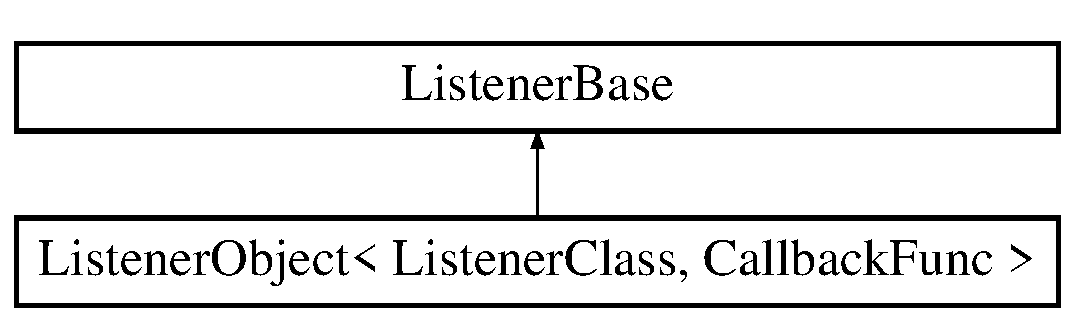
\includegraphics[height=2cm]{classListenerObject}
\end{center}
\end{figure}
\subsection*{Public Member Functions}
\begin{DoxyCompactItemize}
\item 
{\bf ListenerObject} (ListenerClass $\ast$obj, {\bf CallbackFunc} cbf)
\begin{DoxyCompactList}\small\item\em Constructor. \item\end{DoxyCompactList}\item 
virtual {\bf $\sim$ListenerObject} ()
\begin{DoxyCompactList}\small\item\em Destructor. \item\end{DoxyCompactList}\item 
virtual void {\bf invoke} ()
\begin{DoxyCompactList}\small\item\em Callback. \item\end{DoxyCompactList}\end{DoxyCompactItemize}


\subsection{Detailed Description}
\subsubsection*{template$<$class ListenerClass, class CallbackFunc = void (ListenerClass::$\ast$)()$>$ class ListenerObject$<$ ListenerClass, CallbackFunc $>$}

\doxyref{ListenerObject}{p.}{classListenerObject} class. This is a base class for Listener that registers to the timer

\begin{DoxySince}{Since}
0.4.0 
\end{DoxySince}


\subsection{Constructor \& Destructor Documentation}
\index{ListenerObject@{ListenerObject}!ListenerObject@{ListenerObject}}
\index{ListenerObject@{ListenerObject}!ListenerObject@{ListenerObject}}
\subsubsection[{ListenerObject}]{\setlength{\rightskip}{0pt plus 5cm}template$<$class ListenerClass , class CallbackFunc  = void (ListenerClass::$\ast$)()$>$ {\bf ListenerObject}$<$ ListenerClass, {\bf CallbackFunc} $>$::{\bf ListenerObject} (ListenerClass $\ast$ {\em obj}, \/  {\bf CallbackFunc} {\em cbf})\hspace{0.3cm}{\ttfamily  [inline]}}\label{classListenerObject_a53f8500598b1113c1f25e688fce65deb}


Constructor. 

Constructor


\begin{DoxyParams}{Parameters}
\item[{\em obj}]Listener Object \item[{\em cbf}]Callback Function \end{DoxyParams}
\index{ListenerObject@{ListenerObject}!$\sim$ListenerObject@{$\sim$ListenerObject}}
\index{$\sim$ListenerObject@{$\sim$ListenerObject}!ListenerObject@{ListenerObject}}
\subsubsection[{$\sim$ListenerObject}]{\setlength{\rightskip}{0pt plus 5cm}template$<$class ListenerClass , class CallbackFunc  = void (ListenerClass::$\ast$)()$>$ virtual {\bf ListenerObject}$<$ ListenerClass, {\bf CallbackFunc} $>$::$\sim${\bf ListenerObject} ()\hspace{0.3cm}{\ttfamily  [inline, virtual]}}\label{classListenerObject_a17d7197a6efaf43be0e79bb451c65ba9}


Destructor. 

Destructor 

\subsection{Member Function Documentation}
\index{ListenerObject@{ListenerObject}!invoke@{invoke}}
\index{invoke@{invoke}!ListenerObject@{ListenerObject}}
\subsubsection[{invoke}]{\setlength{\rightskip}{0pt plus 5cm}template$<$class ListenerClass , class CallbackFunc  = void (ListenerClass::$\ast$)()$>$ virtual void {\bf ListenerObject}$<$ ListenerClass, {\bf CallbackFunc} $>$::invoke ()\hspace{0.3cm}{\ttfamily  [inline, virtual]}}\label{classListenerObject_a89a5e9d005b8043419f4ccbb244f29d4}


Callback. 

Callback function 

Implements {\bf ListenerBase} \doxyref{}{p.}{classListenerBase_af2cace07df880215fda280ed3cbe0b0b}.


\section{coil::log\_\-stream$<$ \_\-CharT, \_\-Traits $>$ Class Template Reference}
\label{classcoil_1_1log__stream}\index{coil::log\_\-stream@{coil::log\_\-stream}}


\doxyref{log\_\-stream}{p.}{classcoil_1_1log__stream} template class  




{\ttfamily \#include $<$Logger.h$>$}

Inheritance diagram for coil::log\_\-stream$<$ \_\-CharT, \_\-Traits $>$:\begin{figure}[H]
\begin{center}
\leavevmode
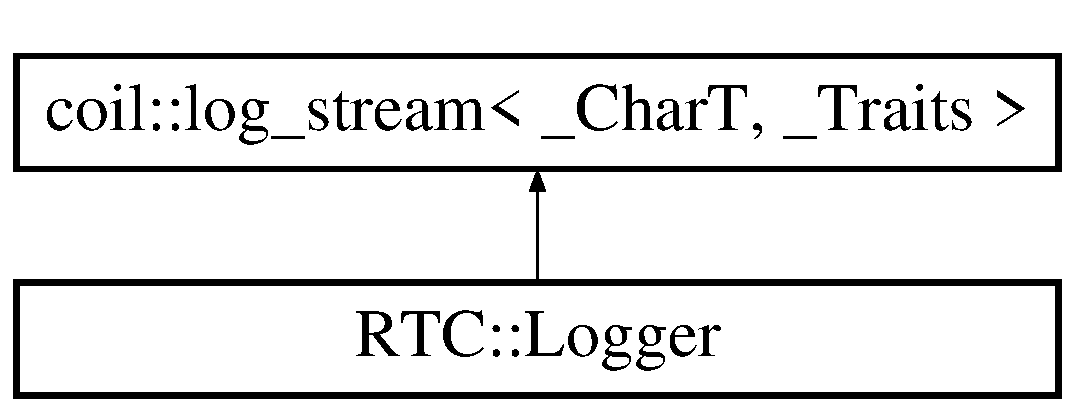
\includegraphics[height=2cm]{classcoil_1_1log__stream}
\end{center}
\end{figure}
\subsection*{Public Types}
\begin{DoxyCompactItemize}
\item 
typedef \_\-CharT {\bf char\_\-type}
\item 
typedef \_\-Traits {\bf traits\_\-type}
\item 
typedef std::basic\_\-ostream$<$ {\bf char\_\-type}, {\bf traits\_\-type} $>$ {\bf ostream\_\-type}
\item 
typedef std::basic\_\-streambuf$<$ {\bf char\_\-type}, {\bf traits\_\-type} $>$ {\bf streambuf\_\-type}
\item 
typedef {\bf coil::Mutex} {\bf Mutex}
\item 
typedef {\bf coil::Guard}$<$ {\bf Mutex} $>$ {\bf Guard}
\end{DoxyCompactItemize}
\subsection*{Public Member Functions}
\begin{DoxyCompactItemize}
\item 
{\bf log\_\-stream} ({\bf streambuf\_\-type} $\ast$sb, int levelmin, int levelmax, int level)
\begin{DoxyCompactList}\small\item\em Constructor. \item\end{DoxyCompactList}\item 
virtual void {\bf header} (int level)
\begin{DoxyCompactList}\small\item\em Message header appender function. \item\end{DoxyCompactList}\item 
bool {\bf setLevel} (int level)
\begin{DoxyCompactList}\small\item\em Set the log level. \item\end{DoxyCompactList}\item 
int {\bf getLevel} () const 
\begin{DoxyCompactList}\small\item\em Get the log level. \item\end{DoxyCompactList}\item 
void {\bf enableLock} ()
\item 
void {\bf disableLock} ()
\item 
{\bf ostream\_\-type} \& {\bf level} (int level)
\begin{DoxyCompactList}\small\item\em Acquire log stream. \item\end{DoxyCompactList}\item 
bool {\bf isValid} (int level) const 
\begin{DoxyCompactList}\small\item\em Log level effective check. \item\end{DoxyCompactList}\item 
void {\bf lock} ()
\begin{DoxyCompactList}\small\item\em Acquire log lock Acquire log lock when the lock mode is set. \item\end{DoxyCompactList}\item 
void {\bf unlock} ()
\begin{DoxyCompactList}\small\item\em Release the log lock Release the log lock when the lock mode is set. \item\end{DoxyCompactList}\end{DoxyCompactItemize}
\subsection*{Static Public Attributes}
\begin{DoxyCompactItemize}
\item 
static bool {\bf m\_\-lockEnable} = true
\begin{DoxyCompactList}\small\item\em Lock enable mode. \item\end{DoxyCompactList}\item 
static {\bf Mutex} {\bf m\_\-mutex}
\begin{DoxyCompactList}\small\item\em Mutual exclusion object. \item\end{DoxyCompactList}\end{DoxyCompactItemize}
\subsection*{Protected Member Functions}
\begin{DoxyCompactItemize}
\item 
{\bf $\sim$log\_\-stream} ()
\begin{DoxyCompactList}\small\item\em Destructor. \item\end{DoxyCompactList}\item 
{\bf log\_\-stream} ()
\begin{DoxyCompactList}\small\item\em Default constructor. \item\end{DoxyCompactList}\item 
{\bf log\_\-stream} (const {\bf log\_\-stream} \&x)
\begin{DoxyCompactList}\small\item\em Copy Constructor. \item\end{DoxyCompactList}\item 
{\bf log\_\-stream} \& {\bf operator=} (const {\bf log\_\-stream} \&x)
\begin{DoxyCompactList}\small\item\em Assignment operator. \item\end{DoxyCompactList}\end{DoxyCompactItemize}


\subsection{Detailed Description}
\subsubsection*{template$<$typename \_\-CharT, typename \_\-Traits = std::char\_\-traits$<$\_\-CharT$>$$>$ class coil::log\_\-stream$<$ \_\-CharT, \_\-Traits $>$}

\doxyref{log\_\-stream}{p.}{classcoil_1_1log__stream} template class 

\subsection{Member Typedef Documentation}
\index{coil::log\_\-stream@{coil::log\_\-stream}!char\_\-type@{char\_\-type}}
\index{char\_\-type@{char\_\-type}!coil::log_stream@{coil::log\_\-stream}}
\subsubsection[{char\_\-type}]{\setlength{\rightskip}{0pt plus 5cm}template$<$typename \_\-CharT , typename \_\-Traits  = std::char\_\-traits$<$\_\-CharT$>$$>$ typedef \_\-CharT {\bf coil::log\_\-stream}$<$ \_\-CharT, \_\-Traits $>$::{\bf char\_\-type}}\label{classcoil_1_1log__stream_a36222157a85ec78d4ef230ab48b346e5}
\index{coil::log\_\-stream@{coil::log\_\-stream}!Guard@{Guard}}
\index{Guard@{Guard}!coil::log_stream@{coil::log\_\-stream}}
\subsubsection[{Guard}]{\setlength{\rightskip}{0pt plus 5cm}template$<$typename \_\-CharT , typename \_\-Traits  = std::char\_\-traits$<$\_\-CharT$>$$>$ typedef {\bf coil::Guard}$<${\bf Mutex}$>$ {\bf coil::log\_\-stream}$<$ \_\-CharT, \_\-Traits $>$::{\bf Guard}}\label{classcoil_1_1log__stream_ae6cc892ef5e4fcf83efd547419566a3b}
\index{coil::log\_\-stream@{coil::log\_\-stream}!Mutex@{Mutex}}
\index{Mutex@{Mutex}!coil::log_stream@{coil::log\_\-stream}}
\subsubsection[{Mutex}]{\setlength{\rightskip}{0pt plus 5cm}template$<$typename \_\-CharT , typename \_\-Traits  = std::char\_\-traits$<$\_\-CharT$>$$>$ typedef {\bf coil::Mutex} {\bf coil::log\_\-stream}$<$ \_\-CharT, \_\-Traits $>$::{\bf Mutex}}\label{classcoil_1_1log__stream_a60cf6ca351d737ffdc17af3313c7a5bb}
\index{coil::log\_\-stream@{coil::log\_\-stream}!ostream\_\-type@{ostream\_\-type}}
\index{ostream\_\-type@{ostream\_\-type}!coil::log_stream@{coil::log\_\-stream}}
\subsubsection[{ostream\_\-type}]{\setlength{\rightskip}{0pt plus 5cm}template$<$typename \_\-CharT , typename \_\-Traits  = std::char\_\-traits$<$\_\-CharT$>$$>$ typedef std::basic\_\-ostream$<${\bf char\_\-type}, {\bf traits\_\-type}$>$ {\bf coil::log\_\-stream}$<$ \_\-CharT, \_\-Traits $>$::{\bf ostream\_\-type}}\label{classcoil_1_1log__stream_a85d8ac9d4a991da58728be6cac8c60cb}
\index{coil::log\_\-stream@{coil::log\_\-stream}!streambuf\_\-type@{streambuf\_\-type}}
\index{streambuf\_\-type@{streambuf\_\-type}!coil::log_stream@{coil::log\_\-stream}}
\subsubsection[{streambuf\_\-type}]{\setlength{\rightskip}{0pt plus 5cm}template$<$typename \_\-CharT , typename \_\-Traits  = std::char\_\-traits$<$\_\-CharT$>$$>$ typedef std::basic\_\-streambuf$<${\bf char\_\-type}, {\bf traits\_\-type}$>$ {\bf coil::log\_\-stream}$<$ \_\-CharT, \_\-Traits $>$::{\bf streambuf\_\-type}}\label{classcoil_1_1log__stream_a24162f3e7cd5e323528e1826b133c960}
\index{coil::log\_\-stream@{coil::log\_\-stream}!traits\_\-type@{traits\_\-type}}
\index{traits\_\-type@{traits\_\-type}!coil::log_stream@{coil::log\_\-stream}}
\subsubsection[{traits\_\-type}]{\setlength{\rightskip}{0pt plus 5cm}template$<$typename \_\-CharT , typename \_\-Traits  = std::char\_\-traits$<$\_\-CharT$>$$>$ typedef \_\-Traits {\bf coil::log\_\-stream}$<$ \_\-CharT, \_\-Traits $>$::{\bf traits\_\-type}}\label{classcoil_1_1log__stream_a89cce42b910a5280d48549dc6e67ebf5}


\subsection{Constructor \& Destructor Documentation}
\index{coil::log\_\-stream@{coil::log\_\-stream}!log\_\-stream@{log\_\-stream}}
\index{log\_\-stream@{log\_\-stream}!coil::log_stream@{coil::log\_\-stream}}
\subsubsection[{log\_\-stream}]{\setlength{\rightskip}{0pt plus 5cm}template$<$typename \_\-CharT , typename \_\-Traits  = std::char\_\-traits$<$\_\-CharT$>$$>$ {\bf coil::log\_\-stream}$<$ \_\-CharT, \_\-Traits $>$::{\bf log\_\-stream} ({\bf streambuf\_\-type} $\ast$ {\em sb}, \/  int {\em levelmin}, \/  int {\em levelmax}, \/  int {\em level})\hspace{0.3cm}{\ttfamily  [inline]}}\label{classcoil_1_1log__stream_a5738d9fec1d931603810307b4b01ea0f}


Constructor. 

Constructor


\begin{DoxyParams}{Parameters}
\item[{\em streambuf}]basic\_\-streambuf type object \item[{\em levelmin}]minimum value for log level \item[{\em levelmax}]maximum value for log level \item[{\em level}]default log level \end{DoxyParams}
\index{coil::log\_\-stream@{coil::log\_\-stream}!$\sim$log\_\-stream@{$\sim$log\_\-stream}}
\index{$\sim$log\_\-stream@{$\sim$log\_\-stream}!coil::log_stream@{coil::log\_\-stream}}
\subsubsection[{$\sim$log\_\-stream}]{\setlength{\rightskip}{0pt plus 5cm}template$<$typename \_\-CharT , typename \_\-Traits  = std::char\_\-traits$<$\_\-CharT$>$$>$ {\bf coil::log\_\-stream}$<$ \_\-CharT, \_\-Traits $>$::$\sim${\bf log\_\-stream} ()\hspace{0.3cm}{\ttfamily  [inline, protected]}}\label{classcoil_1_1log__stream_a6004452bf54de2545bb38537f1063879}


Destructor. 

Destructor \index{coil::log\_\-stream@{coil::log\_\-stream}!log\_\-stream@{log\_\-stream}}
\index{log\_\-stream@{log\_\-stream}!coil::log_stream@{coil::log\_\-stream}}
\subsubsection[{log\_\-stream}]{\setlength{\rightskip}{0pt plus 5cm}template$<$typename \_\-CharT , typename \_\-Traits  = std::char\_\-traits$<$\_\-CharT$>$$>$ {\bf coil::log\_\-stream}$<$ \_\-CharT, \_\-Traits $>$::{\bf log\_\-stream} ()\hspace{0.3cm}{\ttfamily  [protected]}}\label{classcoil_1_1log__stream_a15527816f1dd0c9d1206b936042822d7}


Default constructor. 

Default constructor \index{coil::log\_\-stream@{coil::log\_\-stream}!log\_\-stream@{log\_\-stream}}
\index{log\_\-stream@{log\_\-stream}!coil::log_stream@{coil::log\_\-stream}}
\subsubsection[{log\_\-stream}]{\setlength{\rightskip}{0pt plus 5cm}template$<$typename \_\-CharT , typename \_\-Traits  = std::char\_\-traits$<$\_\-CharT$>$$>$ {\bf coil::log\_\-stream}$<$ \_\-CharT, \_\-Traits $>$::{\bf log\_\-stream} (const {\bf log\_\-stream}$<$ \_\-CharT, \_\-Traits $>$ \& {\em x})\hspace{0.3cm}{\ttfamily  [protected]}}\label{classcoil_1_1log__stream_a63abd81121d608df212526b19fe4384a}


Copy Constructor. 

Copy Constructor


\begin{DoxyParams}{Parameters}
\item[{\em x}]\doxyref{log\_\-stream}{p.}{classcoil_1_1log__stream} object \end{DoxyParams}


\subsection{Member Function Documentation}
\index{coil::log\_\-stream@{coil::log\_\-stream}!disableLock@{disableLock}}
\index{disableLock@{disableLock}!coil::log_stream@{coil::log\_\-stream}}
\subsubsection[{disableLock}]{\setlength{\rightskip}{0pt plus 5cm}template$<$typename \_\-CharT , typename \_\-Traits  = std::char\_\-traits$<$\_\-CharT$>$$>$ void {\bf coil::log\_\-stream}$<$ \_\-CharT, \_\-Traits $>$::disableLock ()\hspace{0.3cm}{\ttfamily  [inline]}}\label{classcoil_1_1log__stream_a5823336515db45fe170d20af2883525c}
Disable the lock mode. 

References coil::log\_\-stream$<$ \_\-CharT, \_\-Traits $>$::m\_\-lockEnable.

\index{coil::log\_\-stream@{coil::log\_\-stream}!enableLock@{enableLock}}
\index{enableLock@{enableLock}!coil::log_stream@{coil::log\_\-stream}}
\subsubsection[{enableLock}]{\setlength{\rightskip}{0pt plus 5cm}template$<$typename \_\-CharT , typename \_\-Traits  = std::char\_\-traits$<$\_\-CharT$>$$>$ void {\bf coil::log\_\-stream}$<$ \_\-CharT, \_\-Traits $>$::enableLock ()\hspace{0.3cm}{\ttfamily  [inline]}}\label{classcoil_1_1log__stream_a31f76626dcd38cc32d10aa17e61198ee}
Enable the lock mode. 

References coil::log\_\-stream$<$ \_\-CharT, \_\-Traits $>$::m\_\-lockEnable.

\index{coil::log\_\-stream@{coil::log\_\-stream}!getLevel@{getLevel}}
\index{getLevel@{getLevel}!coil::log_stream@{coil::log\_\-stream}}
\subsubsection[{getLevel}]{\setlength{\rightskip}{0pt plus 5cm}template$<$typename \_\-CharT , typename \_\-Traits  = std::char\_\-traits$<$\_\-CharT$>$$>$ int {\bf coil::log\_\-stream}$<$ \_\-CharT, \_\-Traits $>$::getLevel () const\hspace{0.3cm}{\ttfamily  [inline]}}\label{classcoil_1_1log__stream_a46361ee727aa32dfb687116a7b411d78}


Get the log level. 

Get the log level.

\begin{DoxyReturn}{Returns}
Log level 
\end{DoxyReturn}
\index{coil::log\_\-stream@{coil::log\_\-stream}!header@{header}}
\index{header@{header}!coil::log_stream@{coil::log\_\-stream}}
\subsubsection[{header}]{\setlength{\rightskip}{0pt plus 5cm}template$<$typename \_\-CharT , typename \_\-Traits  = std::char\_\-traits$<$\_\-CharT$>$$>$ virtual void {\bf coil::log\_\-stream}$<$ \_\-CharT, \_\-Traits $>$::header (int {\em level})\hspace{0.3cm}{\ttfamily  [inline, virtual]}}\label{classcoil_1_1log__stream_acef16b17dc52f988d7f3b28afde3e960}


Message header appender function. 

Subclasses of this class should override this operation, and this function should be defined to append some header to the log messages. 

Reimplemented in {\bf RTC::Logger} \doxyref{}{p.}{classRTC_1_1Logger_a8361781fa7f52ab330c4522bcdd3068b}.



Referenced by coil::log\_\-stream$<$ \_\-CharT, \_\-Traits $>$::level().

\index{coil::log\_\-stream@{coil::log\_\-stream}!isValid@{isValid}}
\index{isValid@{isValid}!coil::log_stream@{coil::log\_\-stream}}
\subsubsection[{isValid}]{\setlength{\rightskip}{0pt plus 5cm}template$<$typename \_\-CharT , typename \_\-Traits  = std::char\_\-traits$<$\_\-CharT$>$$>$ bool {\bf coil::log\_\-stream}$<$ \_\-CharT, \_\-Traits $>$::isValid (int {\em level}) const\hspace{0.3cm}{\ttfamily  [inline]}}\label{classcoil_1_1log__stream_ae48e999605574b2d96c00a51c5cf18df}


Log level effective check. 

Check it whether an appointed log level is an effective range and return effective or invalidity.


\begin{DoxyParams}{Parameters}
\item[{\em level}]Log level\end{DoxyParams}
\begin{DoxyReturn}{Returns}
true: Valid, false: Invalid 
\end{DoxyReturn}
\index{coil::log\_\-stream@{coil::log\_\-stream}!level@{level}}
\index{level@{level}!coil::log_stream@{coil::log\_\-stream}}
\subsubsection[{level}]{\setlength{\rightskip}{0pt plus 5cm}template$<$typename \_\-CharT , typename \_\-Traits  = std::char\_\-traits$<$\_\-CharT$>$$>$ {\bf ostream\_\-type}\& {\bf coil::log\_\-stream}$<$ \_\-CharT, \_\-Traits $>$::level (int {\em level})\hspace{0.3cm}{\ttfamily  [inline]}}\label{classcoil_1_1log__stream_a38cf29e6b6525011bc72510430f3c722}


Acquire log stream. 

Investigate the specified log level and get its log stream. If the specified log level is under the set log level, this class will be returned. If the specified log level exceeds the set log level, a dummy log class will be returned.


\begin{DoxyParams}{Parameters}
\item[{\em level}]The specified log level\end{DoxyParams}
\begin{DoxyReturn}{Returns}
Target log stream 
\end{DoxyReturn}


References coil::log\_\-stream$<$ \_\-CharT, \_\-Traits $>$::header().

\index{coil::log\_\-stream@{coil::log\_\-stream}!lock@{lock}}
\index{lock@{lock}!coil::log_stream@{coil::log\_\-stream}}
\subsubsection[{lock}]{\setlength{\rightskip}{0pt plus 5cm}template$<$typename \_\-CharT , typename \_\-Traits  = std::char\_\-traits$<$\_\-CharT$>$$>$ void {\bf coil::log\_\-stream}$<$ \_\-CharT, \_\-Traits $>$::lock ()\hspace{0.3cm}{\ttfamily  [inline]}}\label{classcoil_1_1log__stream_aec5fa5773666bfda7cb57f3efe208c72}


Acquire log lock Acquire log lock when the lock mode is set. 



References coil::Mutex::lock(), coil::log\_\-stream$<$ \_\-CharT, \_\-Traits $>$::m\_\-lockEnable, and coil::log\_\-stream$<$ \_\-CharT, \_\-Traits $>$::m\_\-mutex.

\index{coil::log\_\-stream@{coil::log\_\-stream}!operator=@{operator=}}
\index{operator=@{operator=}!coil::log_stream@{coil::log\_\-stream}}
\subsubsection[{operator=}]{\setlength{\rightskip}{0pt plus 5cm}template$<$typename \_\-CharT , typename \_\-Traits  = std::char\_\-traits$<$\_\-CharT$>$$>$ {\bf log\_\-stream}\& {\bf coil::log\_\-stream}$<$ \_\-CharT, \_\-Traits $>$::operator= (const {\bf log\_\-stream}$<$ \_\-CharT, \_\-Traits $>$ \& {\em x})\hspace{0.3cm}{\ttfamily  [protected]}}\label{classcoil_1_1log__stream_ab53e7c0b4759cf7f977fb1edd7b21ded}


Assignment operator. 

Copy a \doxyref{log\_\-stream}{p.}{classcoil_1_1log__stream} object.


\begin{DoxyParams}{Parameters}
\item[{\em x}]\doxyref{log\_\-stream}{p.}{classcoil_1_1log__stream} object.\end{DoxyParams}
\begin{DoxyReturn}{Returns}
Assignment result. 
\end{DoxyReturn}
\index{coil::log\_\-stream@{coil::log\_\-stream}!setLevel@{setLevel}}
\index{setLevel@{setLevel}!coil::log_stream@{coil::log\_\-stream}}
\subsubsection[{setLevel}]{\setlength{\rightskip}{0pt plus 5cm}template$<$typename \_\-CharT , typename \_\-Traits  = std::char\_\-traits$<$\_\-CharT$>$$>$ bool {\bf coil::log\_\-stream}$<$ \_\-CharT, \_\-Traits $>$::setLevel (int {\em level})\hspace{0.3cm}{\ttfamily  [inline]}}\label{classcoil_1_1log__stream_a0c8986b423d39003ac210527708df43c}


Set the log level. 

Set the log level.


\begin{DoxyParams}{Parameters}
\item[{\em level}]Log level \end{DoxyParams}
\index{coil::log\_\-stream@{coil::log\_\-stream}!unlock@{unlock}}
\index{unlock@{unlock}!coil::log_stream@{coil::log\_\-stream}}
\subsubsection[{unlock}]{\setlength{\rightskip}{0pt plus 5cm}template$<$typename \_\-CharT , typename \_\-Traits  = std::char\_\-traits$<$\_\-CharT$>$$>$ void {\bf coil::log\_\-stream}$<$ \_\-CharT, \_\-Traits $>$::unlock ()\hspace{0.3cm}{\ttfamily  [inline]}}\label{classcoil_1_1log__stream_ac85f05767b589c323d6b394c8e0ba6af}


Release the log lock Release the log lock when the lock mode is set. 



References coil::log\_\-stream$<$ \_\-CharT, \_\-Traits $>$::m\_\-lockEnable, coil::log\_\-stream$<$ \_\-CharT, \_\-Traits $>$::m\_\-mutex, and coil::Mutex::unlock().



\subsection{Member Data Documentation}
\index{coil::log\_\-stream@{coil::log\_\-stream}!m\_\-lockEnable@{m\_\-lockEnable}}
\index{m\_\-lockEnable@{m\_\-lockEnable}!coil::log_stream@{coil::log\_\-stream}}
\subsubsection[{m\_\-lockEnable}]{\setlength{\rightskip}{0pt plus 5cm}template$<$typename \_\-CharT , typename \_\-Traits  = std::char\_\-traits$<$\_\-CharT$>$$>$ bool {\bf coil::log\_\-stream}$<$ \_\-CharT, \_\-Traits $>$::{\bf m\_\-lockEnable} = true\hspace{0.3cm}{\ttfamily  [inline, static]}}\label{classcoil_1_1log__stream_a128aedc763e4b1d1168069c013b24020}


Lock enable mode. 



Referenced by coil::log\_\-stream$<$ \_\-CharT, \_\-Traits $>$::disableLock(), coil::log\_\-stream$<$ \_\-CharT, \_\-Traits $>$::enableLock(), coil::log\_\-stream$<$ \_\-CharT, \_\-Traits $>$::lock(), and coil::log\_\-stream$<$ \_\-CharT, \_\-Traits $>$::unlock().

\index{coil::log\_\-stream@{coil::log\_\-stream}!m\_\-mutex@{m\_\-mutex}}
\index{m\_\-mutex@{m\_\-mutex}!coil::log_stream@{coil::log\_\-stream}}
\subsubsection[{m\_\-mutex}]{\setlength{\rightskip}{0pt plus 5cm}template$<$typename \_\-CharT , typename \_\-Traits  = std::char\_\-traits$<$\_\-CharT$>$$>$ {\bf coil::Mutex} {\bf coil::log\_\-stream}$<$ \_\-CharT, \_\-Traits $>$::{\bf m\_\-mutex}\hspace{0.3cm}{\ttfamily  [inline, static]}}\label{classcoil_1_1log__stream_a0051fda5ad2fac41d8f2dbd9000b5814}


Mutual exclusion object. 



Referenced by coil::log\_\-stream$<$ \_\-CharT, \_\-Traits $>$::lock(), and coil::log\_\-stream$<$ \_\-CharT, \_\-Traits $>$::unlock().


\section{coil::log\_\-streambuf$<$ \_\-CharT, \_\-Traits $>$ Class Template Reference}
\label{classcoil_1_1log__streambuf}\index{coil::log\_\-streambuf@{coil::log\_\-streambuf}}


\doxyref{log\_\-streambuf}{p.}{classcoil_1_1log__streambuf} template class  




{\ttfamily \#include $<$Logger.h$>$}

\subsection*{Classes}
\begin{DoxyCompactItemize}
\item 
struct {\bf Stream}
\begin{DoxyCompactList}\small\item\em Structure for stream management. \item\end{DoxyCompactList}\end{DoxyCompactItemize}
\subsection*{Public Types}
\begin{DoxyCompactItemize}
\item 
typedef \_\-CharT {\bf char\_\-type}
\item 
typedef \_\-Traits {\bf traits\_\-type}
\item 
typedef std::basic\_\-streambuf$<$ {\bf char\_\-type}, {\bf traits\_\-type} $>$ {\bf streambuf\_\-type}
\item 
typedef {\bf coil::Mutex} {\bf Mutex}
\item 
typedef {\bf coil::Guard}$<$ {\bf coil::Mutex} $>$ {\bf Guard}
\end{DoxyCompactItemize}
\subsection*{Public Member Functions}
\begin{DoxyCompactItemize}
\item 
{\bf log\_\-streambuf} ()
\begin{DoxyCompactList}\small\item\em Constructor. \item\end{DoxyCompactList}\item 
virtual {\bf $\sim$log\_\-streambuf} ()
\begin{DoxyCompactList}\small\item\em Destructor. \item\end{DoxyCompactList}\item 
void {\bf addStream} ({\bf streambuf\_\-type} $\ast$stream, bool cleanup=false)
\begin{DoxyCompactList}\small\item\em Destructor. \item\end{DoxyCompactList}\item 
bool {\bf removeStream} ({\bf streambuf\_\-type} $\ast$stream)
\begin{DoxyCompactList}\small\item\em Destructor. \item\end{DoxyCompactList}\item 
std::vector$<$ {\bf streambuf\_\-type} $\ast$ $>$ {\bf getBuffers} ()
\begin{DoxyCompactList}\small\item\em Get stream buffer list. \item\end{DoxyCompactList}\end{DoxyCompactItemize}
\subsection*{Protected Member Functions}
\begin{DoxyCompactItemize}
\item 
virtual std::streamsize {\bf xsputn} (const {\bf char\_\-type} $\ast$s, std::streamsize n)
\begin{DoxyCompactList}\small\item\em override of basic\_\-streambuf::xsputn \item\end{DoxyCompactList}\item 
virtual std::streamsize {\bf stream\_\-sputn} ()
\begin{DoxyCompactList}\small\item\em Write the stream buffer in stream. \item\end{DoxyCompactList}\item 
virtual std::streamsize {\bf stream\_\-sputn} (const {\bf char\_\-type} $\ast$s, std::streamsize n)
\begin{DoxyCompactList}\small\item\em Writes up to n characters from the array pointed by s to the output sequence controlled by the stream buffer. \item\end{DoxyCompactList}\item 
virtual int {\bf overflow} (int c=traits\_\-type::eof())
\begin{DoxyCompactList}\small\item\em override of basic\_\-streambuf::overflow \item\end{DoxyCompactList}\item 
virtual int {\bf sync} ()
\begin{DoxyCompactList}\small\item\em override of basic\_\-streambuf::sync \item\end{DoxyCompactList}\end{DoxyCompactItemize}


\subsection{Detailed Description}
\subsubsection*{template$<$typename \_\-CharT, typename \_\-Traits = std::char\_\-traits$<$\_\-CharT$>$$>$ class coil::log\_\-streambuf$<$ \_\-CharT, \_\-Traits $>$}

\doxyref{log\_\-streambuf}{p.}{classcoil_1_1log__streambuf} template class 

\subsection{Member Typedef Documentation}
\index{coil::log\_\-streambuf@{coil::log\_\-streambuf}!char\_\-type@{char\_\-type}}
\index{char\_\-type@{char\_\-type}!coil::log_streambuf@{coil::log\_\-streambuf}}
\subsubsection[{char\_\-type}]{\setlength{\rightskip}{0pt plus 5cm}template$<$typename \_\-CharT , typename \_\-Traits  = std::char\_\-traits$<$\_\-CharT$>$$>$ typedef \_\-CharT {\bf coil::log\_\-streambuf}$<$ \_\-CharT, \_\-Traits $>$::{\bf char\_\-type}}\label{classcoil_1_1log__streambuf_a9a97107a5978778f9429e4735f5e85ae}
\index{coil::log\_\-streambuf@{coil::log\_\-streambuf}!Guard@{Guard}}
\index{Guard@{Guard}!coil::log_streambuf@{coil::log\_\-streambuf}}
\subsubsection[{Guard}]{\setlength{\rightskip}{0pt plus 5cm}template$<$typename \_\-CharT , typename \_\-Traits  = std::char\_\-traits$<$\_\-CharT$>$$>$ typedef {\bf coil::Guard}$<${\bf coil::Mutex}$>$ {\bf coil::log\_\-streambuf}$<$ \_\-CharT, \_\-Traits $>$::{\bf Guard}}\label{classcoil_1_1log__streambuf_a740dfbbcd0b7983a7a1ad2c1c371d046}
\index{coil::log\_\-streambuf@{coil::log\_\-streambuf}!Mutex@{Mutex}}
\index{Mutex@{Mutex}!coil::log_streambuf@{coil::log\_\-streambuf}}
\subsubsection[{Mutex}]{\setlength{\rightskip}{0pt plus 5cm}template$<$typename \_\-CharT , typename \_\-Traits  = std::char\_\-traits$<$\_\-CharT$>$$>$ typedef {\bf coil::Mutex} {\bf coil::log\_\-streambuf}$<$ \_\-CharT, \_\-Traits $>$::{\bf Mutex}}\label{classcoil_1_1log__streambuf_a414ef58cbec8134201f3404e5273f8ed}
\index{coil::log\_\-streambuf@{coil::log\_\-streambuf}!streambuf\_\-type@{streambuf\_\-type}}
\index{streambuf\_\-type@{streambuf\_\-type}!coil::log_streambuf@{coil::log\_\-streambuf}}
\subsubsection[{streambuf\_\-type}]{\setlength{\rightskip}{0pt plus 5cm}template$<$typename \_\-CharT , typename \_\-Traits  = std::char\_\-traits$<$\_\-CharT$>$$>$ typedef std::basic\_\-streambuf$<${\bf char\_\-type}, {\bf traits\_\-type}$>$ {\bf coil::log\_\-streambuf}$<$ \_\-CharT, \_\-Traits $>$::{\bf streambuf\_\-type}}\label{classcoil_1_1log__streambuf_a3f1122c7ac61e1e2b89033914ee85b54}
\index{coil::log\_\-streambuf@{coil::log\_\-streambuf}!traits\_\-type@{traits\_\-type}}
\index{traits\_\-type@{traits\_\-type}!coil::log_streambuf@{coil::log\_\-streambuf}}
\subsubsection[{traits\_\-type}]{\setlength{\rightskip}{0pt plus 5cm}template$<$typename \_\-CharT , typename \_\-Traits  = std::char\_\-traits$<$\_\-CharT$>$$>$ typedef \_\-Traits {\bf coil::log\_\-streambuf}$<$ \_\-CharT, \_\-Traits $>$::{\bf traits\_\-type}}\label{classcoil_1_1log__streambuf_a01e45ac5fd741c82e0a39d5e1aac2f47}


\subsection{Constructor \& Destructor Documentation}
\index{coil::log\_\-streambuf@{coil::log\_\-streambuf}!log\_\-streambuf@{log\_\-streambuf}}
\index{log\_\-streambuf@{log\_\-streambuf}!coil::log_streambuf@{coil::log\_\-streambuf}}
\subsubsection[{log\_\-streambuf}]{\setlength{\rightskip}{0pt plus 5cm}template$<$typename \_\-CharT , typename \_\-Traits  = std::char\_\-traits$<$\_\-CharT$>$$>$ {\bf coil::log\_\-streambuf}$<$ \_\-CharT, \_\-Traits $>$::{\bf log\_\-streambuf} ()\hspace{0.3cm}{\ttfamily  [inline]}}\label{classcoil_1_1log__streambuf_aa499e3c876c6222463357e382b344671}


Constructor. 

Constructor 

References BUFFER\_\-LEN.

\index{coil::log\_\-streambuf@{coil::log\_\-streambuf}!$\sim$log\_\-streambuf@{$\sim$log\_\-streambuf}}
\index{$\sim$log\_\-streambuf@{$\sim$log\_\-streambuf}!coil::log_streambuf@{coil::log\_\-streambuf}}
\subsubsection[{$\sim$log\_\-streambuf}]{\setlength{\rightskip}{0pt plus 5cm}template$<$typename \_\-CharT , typename \_\-Traits  = std::char\_\-traits$<$\_\-CharT$>$$>$ virtual {\bf coil::log\_\-streambuf}$<$ \_\-CharT, \_\-Traits $>$::$\sim${\bf log\_\-streambuf} ()\hspace{0.3cm}{\ttfamily  [inline, virtual]}}\label{classcoil_1_1log__streambuf_adfc4bc61eaa1c574bfa8bc6ee23b3136}


Destructor. 

Destructor 

\subsection{Member Function Documentation}
\index{coil::log\_\-streambuf@{coil::log\_\-streambuf}!addStream@{addStream}}
\index{addStream@{addStream}!coil::log_streambuf@{coil::log\_\-streambuf}}
\subsubsection[{addStream}]{\setlength{\rightskip}{0pt plus 5cm}template$<$typename \_\-CharT , typename \_\-Traits  = std::char\_\-traits$<$\_\-CharT$>$$>$ void {\bf coil::log\_\-streambuf}$<$ \_\-CharT, \_\-Traits $>$::addStream ({\bf streambuf\_\-type} $\ast$ {\em stream}, \/  bool {\em cleanup} = {\ttfamily false})\hspace{0.3cm}{\ttfamily  [inline]}}\label{classcoil_1_1log__streambuf_a2a3ecd6335b08209108c4f9558ba9398}


Destructor. 

This operation adds a stream that is actual output stream. User has responsibility to destruct the stream object, since this object never destructs the stream objects. The added stream objects should not be destructed before the destruction of this object. The stream destruction should be done by user after removing it from this object or destructing this object.


\begin{DoxyParams}{Parameters}
\item[{\em stream}]a pointer to std::basic\_\-streambuf type stream object \end{DoxyParams}
\index{coil::log\_\-streambuf@{coil::log\_\-streambuf}!getBuffers@{getBuffers}}
\index{getBuffers@{getBuffers}!coil::log_streambuf@{coil::log\_\-streambuf}}
\subsubsection[{getBuffers}]{\setlength{\rightskip}{0pt plus 5cm}template$<$typename \_\-CharT , typename \_\-Traits  = std::char\_\-traits$<$\_\-CharT$>$$>$ std::vector$<${\bf streambuf\_\-type}$\ast$$>$ {\bf coil::log\_\-streambuf}$<$ \_\-CharT, \_\-Traits $>$::getBuffers ()\hspace{0.3cm}{\ttfamily  [inline]}}\label{classcoil_1_1log__streambuf_a4cc8a12c3925ba73388bf7a897f6498b}


Get stream buffer list. 

Return a stream buffer list.

\begin{DoxyReturn}{Returns}
streambuf\_\-type list 
\end{DoxyReturn}
\index{coil::log\_\-streambuf@{coil::log\_\-streambuf}!overflow@{overflow}}
\index{overflow@{overflow}!coil::log_streambuf@{coil::log\_\-streambuf}}
\subsubsection[{overflow}]{\setlength{\rightskip}{0pt plus 5cm}template$<$typename \_\-CharT , typename \_\-Traits  = std::char\_\-traits$<$\_\-CharT$>$$>$ virtual int {\bf coil::log\_\-streambuf}$<$ \_\-CharT, \_\-Traits $>$::overflow (int {\em c} = {\ttfamily traits\_\-type::eof()})\hspace{0.3cm}{\ttfamily  [inline, protected, virtual]}}\label{classcoil_1_1log__streambuf_adebdd1a8aded503c77efee296f7c3a04}


override of basic\_\-streambuf::overflow 


\begin{DoxyParams}{Parameters}
\item[{\em c}]input character \end{DoxyParams}
\begin{DoxyReturn}{Returns}
return value 
\end{DoxyReturn}


References coil::log\_\-streambuf$<$ \_\-CharT, \_\-Traits $>$::stream\_\-sputn().



Referenced by coil::log\_\-streambuf$<$ \_\-CharT, \_\-Traits $>$::sync().

\index{coil::log\_\-streambuf@{coil::log\_\-streambuf}!removeStream@{removeStream}}
\index{removeStream@{removeStream}!coil::log_streambuf@{coil::log\_\-streambuf}}
\subsubsection[{removeStream}]{\setlength{\rightskip}{0pt plus 5cm}template$<$typename \_\-CharT , typename \_\-Traits  = std::char\_\-traits$<$\_\-CharT$>$$>$ bool {\bf coil::log\_\-streambuf}$<$ \_\-CharT, \_\-Traits $>$::removeStream ({\bf streambuf\_\-type} $\ast$ {\em stream})\hspace{0.3cm}{\ttfamily  [inline]}}\label{classcoil_1_1log__streambuf_a1704c352e01cc833612690e3bbc67b68}


Destructor. 

This operation remove a stream that is actual output stream. User has responsibility to destruct the stream object.


\begin{DoxyParams}{Parameters}
\item[{\em stream}]a pointer to std::basic\_\-streambuf type stream object \end{DoxyParams}
\begin{DoxyReturn}{Returns}
Whether removing the stream succeeded. 
\end{DoxyReturn}
\index{coil::log\_\-streambuf@{coil::log\_\-streambuf}!stream\_\-sputn@{stream\_\-sputn}}
\index{stream\_\-sputn@{stream\_\-sputn}!coil::log_streambuf@{coil::log\_\-streambuf}}
\subsubsection[{stream\_\-sputn}]{\setlength{\rightskip}{0pt plus 5cm}template$<$typename \_\-CharT , typename \_\-Traits  = std::char\_\-traits$<$\_\-CharT$>$$>$ virtual std::streamsize {\bf coil::log\_\-streambuf}$<$ \_\-CharT, \_\-Traits $>$::stream\_\-sputn (const {\bf char\_\-type} $\ast$ {\em s}, \/  std::streamsize {\em n})\hspace{0.3cm}{\ttfamily  [inline, protected, virtual]}}\label{classcoil_1_1log__streambuf_acd1e28861820f7fd8065c32eef65f04d}


Writes up to n characters from the array pointed by s to the output sequence controlled by the stream buffer. 


\begin{DoxyParams}{Parameters}
\item[{\em s}]a pointer to input characters \item[{\em n}]number of input characters \end{DoxyParams}
\begin{DoxyReturn}{Returns}
The number of characters written. 
\end{DoxyReturn}
\index{coil::log\_\-streambuf@{coil::log\_\-streambuf}!stream\_\-sputn@{stream\_\-sputn}}
\index{stream\_\-sputn@{stream\_\-sputn}!coil::log_streambuf@{coil::log\_\-streambuf}}
\subsubsection[{stream\_\-sputn}]{\setlength{\rightskip}{0pt plus 5cm}template$<$typename \_\-CharT , typename \_\-Traits  = std::char\_\-traits$<$\_\-CharT$>$$>$ virtual std::streamsize {\bf coil::log\_\-streambuf}$<$ \_\-CharT, \_\-Traits $>$::stream\_\-sputn ()\hspace{0.3cm}{\ttfamily  [inline, protected, virtual]}}\label{classcoil_1_1log__streambuf_a9f8cef21f4ea01f154ef5520513d60ea}


Write the stream buffer in stream. 

\begin{DoxyReturn}{Returns}
The number of characters written. 
\end{DoxyReturn}


Referenced by coil::log\_\-streambuf$<$ \_\-CharT, \_\-Traits $>$::overflow(), coil::log\_\-streambuf$<$ \_\-CharT, \_\-Traits $>$::sync(), and coil::log\_\-streambuf$<$ \_\-CharT, \_\-Traits $>$::xsputn().

\index{coil::log\_\-streambuf@{coil::log\_\-streambuf}!sync@{sync}}
\index{sync@{sync}!coil::log_streambuf@{coil::log\_\-streambuf}}
\subsubsection[{sync}]{\setlength{\rightskip}{0pt plus 5cm}template$<$typename \_\-CharT , typename \_\-Traits  = std::char\_\-traits$<$\_\-CharT$>$$>$ virtual int {\bf coil::log\_\-streambuf}$<$ \_\-CharT, \_\-Traits $>$::sync ()\hspace{0.3cm}{\ttfamily  [inline, protected, virtual]}}\label{classcoil_1_1log__streambuf_a1b973de50d8021dd19c200afc6067562}


override of basic\_\-streambuf::sync 

\begin{DoxyReturn}{Returns}
return value 
\end{DoxyReturn}


References coil::log\_\-streambuf$<$ \_\-CharT, \_\-Traits $>$::overflow(), and coil::log\_\-streambuf$<$ \_\-CharT, \_\-Traits $>$::stream\_\-sputn().

\index{coil::log\_\-streambuf@{coil::log\_\-streambuf}!xsputn@{xsputn}}
\index{xsputn@{xsputn}!coil::log_streambuf@{coil::log\_\-streambuf}}
\subsubsection[{xsputn}]{\setlength{\rightskip}{0pt plus 5cm}template$<$typename \_\-CharT , typename \_\-Traits  = std::char\_\-traits$<$\_\-CharT$>$$>$ virtual std::streamsize {\bf coil::log\_\-streambuf}$<$ \_\-CharT, \_\-Traits $>$::xsputn (const {\bf char\_\-type} $\ast$ {\em s}, \/  std::streamsize {\em n})\hspace{0.3cm}{\ttfamily  [inline, protected, virtual]}}\label{classcoil_1_1log__streambuf_a113d3c59f9616c432bb182705efa3bc6}


override of basic\_\-streambuf::xsputn 


\begin{DoxyParams}{Parameters}
\item[{\em s}]a pointer to input characters \item[{\em n}]number of input characters \end{DoxyParams}
\begin{DoxyReturn}{Returns}
input stream size 
\end{DoxyReturn}


References coil::log\_\-streambuf$<$ \_\-CharT, \_\-Traits $>$::stream\_\-sputn().


\section{クラス RTC::Logger}
\label{classRTC_1_1Logger}\index{RTC::Logger@{RTC::Logger}}


\doxyref{Logger}{p.}{classRTC_1_1Logger} クラス.  




{\ttfamily \#include $<$SystemLogger.h$>$}

RTC::Loggerに対する継承グラフ\begin{figure}[H]
\begin{center}
\leavevmode
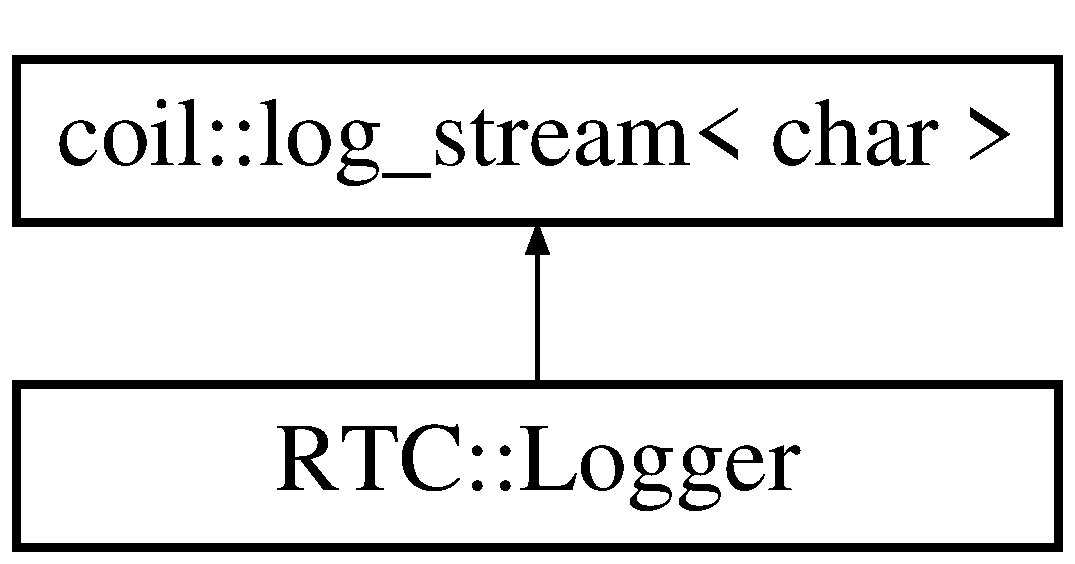
\includegraphics[height=2cm]{classRTC_1_1Logger}
\end{center}
\end{figure}
\subsection*{Public 型}
\begin{DoxyCompactItemize}
\item 
enum \{ \par
{\bf RTL\_\-SILENT}, 
{\bf RTL\_\-FATAL}, 
{\bf RTL\_\-ERROR}, 
{\bf RTL\_\-WARN}, 
\par
{\bf RTL\_\-INFO}, 
{\bf RTL\_\-DEBUG}, 
{\bf RTL\_\-TRACE}, 
{\bf RTL\_\-VERBOSE}, 
\par
{\bf RTL\_\-PARANOID}
 \}
\end{DoxyCompactItemize}
\subsection*{Public メソッド}
\begin{DoxyCompactItemize}
\item 
{\bf Logger} (const char $\ast$name=\char`\"{}\char`\"{})
\begin{DoxyCompactList}\small\item\em コンストラクタ \item\end{DoxyCompactList}\item 
{\bf Logger} ({\bf LogStreamBuf} $\ast$streambuf)
\begin{DoxyCompactList}\small\item\em コンストラクタ \item\end{DoxyCompactList}\item 
virtual {\bf $\sim$Logger} (void)
\begin{DoxyCompactList}\small\item\em 仮想デストラクタ \item\end{DoxyCompactList}\item 
bool {\bf setLevel} (const char $\ast$level)
\begin{DoxyCompactList}\small\item\em ログレベルを文字列で設定する \item\end{DoxyCompactList}\item 
void {\bf setDateFormat} (const char $\ast$format)
\begin{DoxyCompactList}\small\item\em ヘッダに付加する日時フォーマットを指定する。 \item\end{DoxyCompactList}\item 
void {\bf setName} (const char $\ast$name)
\begin{DoxyCompactList}\small\item\em ヘッダの日時の後に付加する文字列を設定する。 \item\end{DoxyCompactList}\end{DoxyCompactItemize}
\subsection*{Protected メソッド}
\begin{DoxyCompactItemize}
\item 
virtual void {\bf header} (int level)
\begin{DoxyCompactList}\small\item\em メッセージのプリフィックス追加関数 \item\end{DoxyCompactList}\item 
std::string {\bf getDate} (void)
\begin{DoxyCompactList}\small\item\em フォーマットされた現在日時文字列を取得する。 指定された書式で記述した現在日時を取得する。 \item\end{DoxyCompactList}\item 
int {\bf strToLevel} (const char $\ast$level)
\begin{DoxyCompactList}\small\item\em ログレベル設定 与えられた文字列に対応したログレベルを設定する。 \item\end{DoxyCompactList}\end{DoxyCompactItemize}


\subsection{説明}
\doxyref{Logger}{p.}{classRTC_1_1Logger} クラス. 
\begin{DoxyItemize}
\item ログ出力をシリアライズしかつ分配するバッファクラス
\item ログをフォーマットするフォーマットクラス で構成されるロガークラス
\end{DoxyItemize}


\begin{DoxyItemize}
\item バッファクラス
\begin{DoxyItemize}
\item マルチスレッド書き込みに対してシリアライズしてバッファリングする
\item 複数の出力先にログを出力できる
\item 出力先の例としては、ファイル、標準出力、リモートのログサーバ等
\item バッファに対してaddStreamで出力先を追加できる
\end{DoxyItemize}
\item フォーマットクラス
\begin{DoxyItemize}
\item ログレベルを指定して出力できる
\item 書式は、[時間] [ログレベル] [サフィックス] [メッセージ]
\item [時間] [ログレベル] [サフィックス]は自動付加
\item [サフィックス] を指定できる関数を用意
\item ログレベルは以下のとおり
\begin{DoxyItemize}
\item RTL\_\-SILENT
\item RTL\_\-FATAL
\item RTL\_\-ERROR
\item RTL\_\-WARN
\item RTL\_\-INFO
\item RTL\_\-DEBUG
\item RTL\_\-TRACE
\item RTL\_\-VERBOSE
\item RTL\_\-PARANOID
\end{DoxyItemize}
\item このフォーマットオブジェクトに対するロック・アンロック機能 
\end{DoxyItemize}
\end{DoxyItemize}

\subsection{列挙型}
\subsubsection[{"@0}]{\setlength{\rightskip}{0pt plus 5cm}anonymous enum}\label{classRTC_1_1Logger_a26c3dbf0a4c0fa3c4cc5e3a472636879}
\begin{Desc}
\item[列挙型の値: ]\par
\begin{description}
\index{RTL\_\-SILENT@{RTL\_\-SILENT}!RTC::Logger@{RTC::Logger}}\index{RTC::Logger@{RTC::Logger}!RTL\_\-SILENT@{RTL\_\-SILENT}}\item[{\em 
RTL\_\-SILENT\label{classRTC_1_1Logger_a26c3dbf0a4c0fa3c4cc5e3a472636879a3367cbfc4e33871c5fa76fd1cd36756a}
}]\index{RTL\_\-FATAL@{RTL\_\-FATAL}!RTC::Logger@{RTC::Logger}}\index{RTC::Logger@{RTC::Logger}!RTL\_\-FATAL@{RTL\_\-FATAL}}\item[{\em 
RTL\_\-FATAL\label{classRTC_1_1Logger_a26c3dbf0a4c0fa3c4cc5e3a472636879a7fe2f71dc262f90d320099edb7c16087}
}]\index{RTL\_\-ERROR@{RTL\_\-ERROR}!RTC::Logger@{RTC::Logger}}\index{RTC::Logger@{RTC::Logger}!RTL\_\-ERROR@{RTL\_\-ERROR}}\item[{\em 
RTL\_\-ERROR\label{classRTC_1_1Logger_a26c3dbf0a4c0fa3c4cc5e3a472636879ac99eb1601f28452bc182c2d86a1029a0}
}]\index{RTL\_\-WARN@{RTL\_\-WARN}!RTC::Logger@{RTC::Logger}}\index{RTC::Logger@{RTC::Logger}!RTL\_\-WARN@{RTL\_\-WARN}}\item[{\em 
RTL\_\-WARN\label{classRTC_1_1Logger_a26c3dbf0a4c0fa3c4cc5e3a472636879a519a7175117c1fe1e4d37950f56437ba}
}]\index{RTL\_\-INFO@{RTL\_\-INFO}!RTC::Logger@{RTC::Logger}}\index{RTC::Logger@{RTC::Logger}!RTL\_\-INFO@{RTL\_\-INFO}}\item[{\em 
RTL\_\-INFO\label{classRTC_1_1Logger_a26c3dbf0a4c0fa3c4cc5e3a472636879a14e025e496dafbec620acc01f3df9ef5}
}]\index{RTL\_\-DEBUG@{RTL\_\-DEBUG}!RTC::Logger@{RTC::Logger}}\index{RTC::Logger@{RTC::Logger}!RTL\_\-DEBUG@{RTL\_\-DEBUG}}\item[{\em 
RTL\_\-DEBUG\label{classRTC_1_1Logger_a26c3dbf0a4c0fa3c4cc5e3a472636879a1d7ef00333c4c80a9a726d9d33b428e0}
}]\index{RTL\_\-TRACE@{RTL\_\-TRACE}!RTC::Logger@{RTC::Logger}}\index{RTC::Logger@{RTC::Logger}!RTL\_\-TRACE@{RTL\_\-TRACE}}\item[{\em 
RTL\_\-TRACE\label{classRTC_1_1Logger_a26c3dbf0a4c0fa3c4cc5e3a472636879af6a89134b5b95f2f4b4fb6cf2c631b54}
}]\index{RTL\_\-VERBOSE@{RTL\_\-VERBOSE}!RTC::Logger@{RTC::Logger}}\index{RTC::Logger@{RTC::Logger}!RTL\_\-VERBOSE@{RTL\_\-VERBOSE}}\item[{\em 
RTL\_\-VERBOSE\label{classRTC_1_1Logger_a26c3dbf0a4c0fa3c4cc5e3a472636879abdbd3de57d4b10ba4e8f19f601619378}
}]\index{RTL\_\-PARANOID@{RTL\_\-PARANOID}!RTC::Logger@{RTC::Logger}}\index{RTC::Logger@{RTC::Logger}!RTL\_\-PARANOID@{RTL\_\-PARANOID}}\item[{\em 
RTL\_\-PARANOID\label{classRTC_1_1Logger_a26c3dbf0a4c0fa3c4cc5e3a472636879ac9bd2a83ac9b45acba1e71b2cd3b9fad}
}]\end{description}
\end{Desc}



\subsection{コンストラクタとデストラクタ}
\index{RTC::Logger@{RTC::Logger}!Logger@{Logger}}
\index{Logger@{Logger}!RTC::Logger@{RTC::Logger}}
\subsubsection[{Logger}]{\setlength{\rightskip}{0pt plus 5cm}RTC::Logger::Logger (const char $\ast$ {\em name} = {\ttfamily \char`\"{}\char`\"{}})}\label{classRTC_1_1Logger_ab2e8e5300567b89edc7586f41e184c5b}


コンストラクタ 

コンストラクタ


\begin{DoxyParams}{引数}
\item[{\em name}]ヘッダの日時の後に付加する文字列 \end{DoxyParams}
\index{RTC::Logger@{RTC::Logger}!Logger@{Logger}}
\index{Logger@{Logger}!RTC::Logger@{RTC::Logger}}
\subsubsection[{Logger}]{\setlength{\rightskip}{0pt plus 5cm}RTC::Logger::Logger ({\bf LogStreamBuf} $\ast$ {\em streambuf})}\label{classRTC_1_1Logger_a201ebea93493a822bef5397b0666c1f3}


コンストラクタ 

コンストラクタ


\begin{DoxyParams}{引数}
\item[{\em streambuf}]LogStream オブジェクト \end{DoxyParams}
\index{RTC::Logger@{RTC::Logger}!$\sim$Logger@{$\sim$Logger}}
\index{$\sim$Logger@{$\sim$Logger}!RTC::Logger@{RTC::Logger}}
\subsubsection[{$\sim$Logger}]{\setlength{\rightskip}{0pt plus 5cm}virtual RTC::Logger::$\sim$Logger (void)\hspace{0.3cm}{\ttfamily  [virtual]}}\label{classRTC_1_1Logger_a4cc391947ae2c203773216049b6a658d}


仮想デストラクタ 



\subsection{関数}
\index{RTC::Logger@{RTC::Logger}!getDate@{getDate}}
\index{getDate@{getDate}!RTC::Logger@{RTC::Logger}}
\subsubsection[{getDate}]{\setlength{\rightskip}{0pt plus 5cm}std::string RTC::Logger::getDate (void)\hspace{0.3cm}{\ttfamily  [protected]}}\label{classRTC_1_1Logger_afd3ce56caeea1d4cb12725b4c0905aec}


フォーマットされた現在日時文字列を取得する。 指定された書式で記述した現在日時を取得する。 

\begin{DoxyReturn}{戻り値}
書式指定現在日時 
\end{DoxyReturn}
\index{RTC::Logger@{RTC::Logger}!header@{header}}
\index{header@{header}!RTC::Logger@{RTC::Logger}}
\subsubsection[{header}]{\setlength{\rightskip}{0pt plus 5cm}virtual void RTC::Logger::header (int {\em level})\hspace{0.3cm}{\ttfamily  [protected, virtual]}}\label{classRTC_1_1Logger_a8361781fa7f52ab330c4522bcdd3068b}


メッセージのプリフィックス追加関数 

サブクラスにおいてこの関数をオーバーライドし、 ログメッセージに適当なプリフィックスるを追加する。 

{\bf coil::log\_\-stream$<$ \_\-CharT, \_\-Traits $>$} \doxyref{}{p.}{classcoil_1_1log__stream_acef16b17dc52f988d7f3b28afde3e960}を再定義しています。

\index{RTC::Logger@{RTC::Logger}!setDateFormat@{setDateFormat}}
\index{setDateFormat@{setDateFormat}!RTC::Logger@{RTC::Logger}}
\subsubsection[{setDateFormat}]{\setlength{\rightskip}{0pt plus 5cm}void RTC::Logger::setDateFormat (const char $\ast$ {\em format})}\label{classRTC_1_1Logger_a5479637be023b33f41a75894806887b7}


ヘッダに付加する日時フォーマットを指定する。 

フォーマット指定文字列は以下のとおり。 
\begin{DoxyPre}
 \%a abbreviated weekday name 
 \%A full weekday name 
 \%b abbreviated month name 
 \%B full month name 
 \%c the standard date and time string 
 \%d day of the month, as a number (1-31) 
 \%H hour, 24 hour format (0-23) 
 \%I hour, 12 hour format (1-12) 
 \%j day of the year, as a number (1-366) 
 \%m month as a number (1-12).
    Note: some versions of Microsoft Visual C++ may use values that range
    from 0-11. 
 \%M minute as a number (0-59) 
 \%p locale's equivalent of AM or PM 
 \%Q millisecond as a number (0-999) from ver 1.1
 \%q microsecond as a number (0-999) from ver 1.1
 \%S second as a number (0-59) 
 \%U week of the year, sunday as the first day 
 \%w weekday as a decimal (0-6, sunday=0) 
 \%W week of the year, monday as the first day 
 \%x standard date string 
 \%X standard time string 
 \%y year in decimal, without the century (0-99) 
 \%Y year in decimal, with the century 
 \%Z time zone name 
 \%\% a percent sign 
 \end{DoxyPre}



\begin{DoxyParams}{引数}
\item[{\em fmt}]日時フォーマット \end{DoxyParams}
\index{RTC::Logger@{RTC::Logger}!setLevel@{setLevel}}
\index{setLevel@{setLevel}!RTC::Logger@{RTC::Logger}}
\subsubsection[{setLevel}]{\setlength{\rightskip}{0pt plus 5cm}bool RTC::Logger::setLevel (const char $\ast$ {\em level})}\label{classRTC_1_1Logger_abfc5decf1819d5e5fbd9d4f755c6d9a3}


ログレベルを文字列で設定する 


\begin{DoxyParams}{引数}
\item[{\em level}]ログレベル \end{DoxyParams}
\index{RTC::Logger@{RTC::Logger}!setName@{setName}}
\index{setName@{setName}!RTC::Logger@{RTC::Logger}}
\subsubsection[{setName}]{\setlength{\rightskip}{0pt plus 5cm}void RTC::Logger::setName (const char $\ast$ {\em name})}\label{classRTC_1_1Logger_a4a7b805b7d950cdc4eed64565a7a62d3}


ヘッダの日時の後に付加する文字列を設定する。 

ヘッダの日時の後に付加する接頭語文字列を設定する。


\begin{DoxyParams}{引数}
\item[{\em suffix}]接頭語文字列 \end{DoxyParams}
\index{RTC::Logger@{RTC::Logger}!strToLevel@{strToLevel}}
\index{strToLevel@{strToLevel}!RTC::Logger@{RTC::Logger}}
\subsubsection[{strToLevel}]{\setlength{\rightskip}{0pt plus 5cm}int RTC::Logger::strToLevel (const char $\ast$ {\em level})\hspace{0.3cm}{\ttfamily  [protected]}}\label{classRTC_1_1Logger_a684f47d977da5a696021137583852407}


ログレベル設定 与えられた文字列に対応したログレベルを設定する。 


\begin{DoxyParams}{引数}
\item[{\em lv}]ログレベル文字列 \end{DoxyParams}
\begin{DoxyReturn}{戻り値}
設定したログレベル 
\end{DoxyReturn}

\section{RTC::Manager Class Reference}
\label{classRTC_1_1Manager}\index{RTC::Manager@{RTC::Manager}}


\doxyref{Manager}{p.}{classRTC_1_1Manager} class.  




{\ttfamily \#include $<$Manager.h$>$}

\subsection*{Classes}
\begin{DoxyCompactItemize}
\item 
struct {\bf ECFactoryPredicate}
\item 
class {\bf FactoryPredicate}
\item 
struct {\bf Finalized}
\item 
struct {\bf InstanceName}
\item 
struct {\bf ModuleFactories}
\item 
class {\bf ModulePredicate}
\item 
class {\bf OrbRunner}
\begin{DoxyCompactList}\small\item\em \doxyref{OrbRunner}{p.}{classRTC_1_1Manager_1_1OrbRunner} class. \item\end{DoxyCompactList}\item 
struct {\bf Term}
\item 
class {\bf Terminator}
\begin{DoxyCompactList}\small\item\em \doxyref{Terminator}{p.}{classRTC_1_1Manager_1_1Terminator} class. \item\end{DoxyCompactList}\end{DoxyCompactItemize}
\subsection*{Public Member Functions}
\begin{DoxyCompactItemize}
\item 
void {\bf terminate} ()
\begin{DoxyCompactList}\small\item\em Terminate manager. \item\end{DoxyCompactList}\item 
void {\bf shutdown} ()
\begin{DoxyCompactList}\small\item\em Shutdown \doxyref{Manager}{p.}{classRTC_1_1Manager}. \item\end{DoxyCompactList}\item 
void {\bf join} ()
\begin{DoxyCompactList}\small\item\em Wait for Manager's termination. \item\end{DoxyCompactList}\item 
{\bf LogStreamBuf} \& {\bf getLogStreamBuf} ()
\begin{DoxyCompactList}\small\item\em Get the log buffer. \item\end{DoxyCompactList}\item 
std::string \& {\bf getLogLevel} ()
\begin{DoxyCompactList}\small\item\em Get the log level of the configuration. \item\end{DoxyCompactList}\item 
{\bf coil::Properties} \& {\bf getConfig} ()
\begin{DoxyCompactList}\small\item\em Get the manager configuration. \item\end{DoxyCompactList}\item 
void {\bf setModuleInitProc} ({\bf ModuleInitProc} proc)
\begin{DoxyCompactList}\small\item\em Set initial procedure. \item\end{DoxyCompactList}\item 
bool {\bf activateManager} ()
\begin{DoxyCompactList}\small\item\em Activate the \doxyref{Manager}{p.}{classRTC_1_1Manager}. \item\end{DoxyCompactList}\item 
void {\bf runManager} (bool no\_\-block=false)
\begin{DoxyCompactList}\small\item\em Run the \doxyref{Manager}{p.}{classRTC_1_1Manager}. \item\end{DoxyCompactList}\item 
void {\bf load} (const char $\ast$fname, const char $\ast$initfunc)
\begin{DoxyCompactList}\small\item\em [CORBA interface] Load module \item\end{DoxyCompactList}\item 
void {\bf unload} (const char $\ast$fname)
\begin{DoxyCompactList}\small\item\em Unload module. \item\end{DoxyCompactList}\item 
void {\bf unloadAll} ()
\item 
std::vector$<$ {\bf coil::Properties} $>$ {\bf getLoadedModules} ()
\begin{DoxyCompactList}\small\item\em Get a list of loaded modules. \item\end{DoxyCompactList}\item 
std::vector$<$ {\bf coil::Properties} $>$ {\bf getLoadableModules} ()
\begin{DoxyCompactList}\small\item\em Get a list of loadable modules. \item\end{DoxyCompactList}\item 
bool {\bf registerFactory} ({\bf coil::Properties} \&profile, {\bf RtcNewFunc} new\_\-func, {\bf RtcDeleteFunc} delete\_\-func)
\begin{DoxyCompactList}\small\item\em Register RT-\/Component Factory. \item\end{DoxyCompactList}\item 
std::vector$<$ {\bf coil::Properties} $>$ {\bf getFactoryProfiles} ()
\begin{DoxyCompactList}\small\item\em Get profiles of factories. \item\end{DoxyCompactList}\item 
bool {\bf registerECFactory} (const char $\ast$name, {\bf ECNewFunc} new\_\-func, {\bf ECDeleteFunc} delete\_\-func)
\begin{DoxyCompactList}\small\item\em Register ExecutionContext Factory. \item\end{DoxyCompactList}\item 
std::vector$<$ std::string $>$ {\bf getModulesFactories} ()
\begin{DoxyCompactList}\small\item\em Get the list of all Factories. \item\end{DoxyCompactList}\item 
{\bf RTObject\_\-impl} $\ast$ {\bf createComponent} (const char $\ast$comp\_\-args)
\begin{DoxyCompactList}\small\item\em Create RT-\/Components. \item\end{DoxyCompactList}\item 
{\bf ExecutionContextBase} $\ast$ {\bf createContext} (const char $\ast$ec\_\-args)
\begin{DoxyCompactList}\small\item\em Create Context. \item\end{DoxyCompactList}\item 
void {\bf cleanupComponent} ({\bf RTObject\_\-impl} $\ast$comp)
\begin{DoxyCompactList}\small\item\em Unregister RT-\/Components. \item\end{DoxyCompactList}\item 
void {\bf cleanupComponents} ()
\begin{DoxyCompactList}\small\item\em This method deletes RT-\/Components. \item\end{DoxyCompactList}\item 
void {\bf notifyFinalized} ({\bf RTObject\_\-impl} $\ast$comp)
\begin{DoxyCompactList}\small\item\em This method deletes RT-\/Components. \item\end{DoxyCompactList}\item 
bool {\bf registerComponent} ({\bf RTObject\_\-impl} $\ast$comp)
\begin{DoxyCompactList}\small\item\em Register RT-\/Component directly without Factory. \item\end{DoxyCompactList}\item 
bool {\bf unregisterComponent} ({\bf RTObject\_\-impl} $\ast$comp)
\begin{DoxyCompactList}\small\item\em Unregister RT-\/Components. \item\end{DoxyCompactList}\item 
void {\bf deleteComponent} ({\bf RTObject\_\-impl} $\ast$comp)
\begin{DoxyCompactList}\small\item\em Unregister RT-\/Components that have been registered to \doxyref{Manager}{p.}{classRTC_1_1Manager}. \item\end{DoxyCompactList}\item 
void {\bf deleteComponent} (const char $\ast$instance\_\-name)
\begin{DoxyCompactList}\small\item\em Unregister RT-\/Components that have been registered to \doxyref{Manager}{p.}{classRTC_1_1Manager}. \item\end{DoxyCompactList}\item 
{\bf RTObject\_\-impl} $\ast$ {\bf getComponent} (const char $\ast$instance\_\-name)
\begin{DoxyCompactList}\small\item\em Get RT-\/Component's pointer. \item\end{DoxyCompactList}\item 
std::vector$<$ {\bf RTObject\_\-impl} $\ast$ $>$ {\bf getComponents} ()
\begin{DoxyCompactList}\small\item\em Get all RT-\/Components registered in the \doxyref{Manager}{p.}{classRTC_1_1Manager}. \item\end{DoxyCompactList}\item 
CORBA::ORB\_\-ptr {\bf getORB} ()
\begin{DoxyCompactList}\small\item\em Get the pointer to ORB. \item\end{DoxyCompactList}\item 
PortableServer::POA\_\-ptr {\bf getPOA} ()
\begin{DoxyCompactList}\small\item\em Get a pointer to RootPOA held by \doxyref{Manager}{p.}{classRTC_1_1Manager}. \item\end{DoxyCompactList}\item 
PortableServer::POAManager\_\-ptr {\bf getPOAManager} ()
\begin{DoxyCompactList}\small\item\em Get POAManager that \doxyref{Manager}{p.}{classRTC_1_1Manager} has. \item\end{DoxyCompactList}\end{DoxyCompactItemize}
\subsection*{Static Public Member Functions}
\begin{DoxyCompactItemize}
\item 
static {\bf Manager} $\ast$ {\bf init} (int argc, char $\ast$$\ast$argv)
\begin{DoxyCompactList}\small\item\em Initialize manager. \item\end{DoxyCompactList}\item 
static {\bf Manager} \& {\bf instance} ()
\begin{DoxyCompactList}\small\item\em Get instance of the manager. \item\end{DoxyCompactList}\end{DoxyCompactItemize}
\subsection*{Protected Types}
\begin{DoxyCompactItemize}
\item 
typedef {\bf ObjectManager}$<$ std::string, {\bf RTObject\_\-impl}, {\bf InstanceName} $>$ {\bf ComponentManager}
\item 
typedef {\bf ObjectManager}$<$ const {\bf coil::Properties}, {\bf FactoryBase}, {\bf FactoryPredicate} $>$ {\bf FactoryManager}
\begin{DoxyCompactList}\small\item\em ComponentFactory. \item\end{DoxyCompactList}\item 
typedef {\bf ObjectManager}$<$ const char $\ast$, {\bf ECFactoryBase}, {\bf ECFactoryPredicate} $>$ {\bf ECFactoryManager}
\end{DoxyCompactItemize}
\subsection*{Protected Member Functions}
\begin{DoxyCompactItemize}
\item 
{\bf Manager} ()
\begin{DoxyCompactList}\small\item\em Protected Constructor. \item\end{DoxyCompactList}\item 
{\bf Manager} (const {\bf Manager} \&{\bf manager})
\begin{DoxyCompactList}\small\item\em Protected Copy Constructor. \item\end{DoxyCompactList}\item 
void {\bf initManager} (int argc, char $\ast$$\ast$argv)
\begin{DoxyCompactList}\small\item\em \doxyref{Manager}{p.}{classRTC_1_1Manager} internal initialization. \item\end{DoxyCompactList}\item 
void {\bf shutdownManager} ()
\begin{DoxyCompactList}\small\item\em Shutdown \doxyref{Manager}{p.}{classRTC_1_1Manager}. \item\end{DoxyCompactList}\item 
void {\bf shutdownOnNoRtcs} ()
\begin{DoxyCompactList}\small\item\em Shutdown \doxyref{Manager}{p.}{classRTC_1_1Manager}. \item\end{DoxyCompactList}\item 
bool {\bf initLogger} ()
\begin{DoxyCompactList}\small\item\em System logger initialization. \item\end{DoxyCompactList}\item 
void {\bf shutdownLogger} ()
\begin{DoxyCompactList}\small\item\em System \doxyref{Logger}{p.}{classRTC_1_1Logger} finalization. \item\end{DoxyCompactList}\item 
bool {\bf initORB} ()
\begin{DoxyCompactList}\small\item\em CORBA ORB initialization. \item\end{DoxyCompactList}\item 
std::string {\bf createORBOptions} ()
\begin{DoxyCompactList}\small\item\em Create ORB command options. \item\end{DoxyCompactList}\item 
void {\bf createORBEndpoints} ({\bf coil::vstring} \&endpoints)
\begin{DoxyCompactList}\small\item\em Create Endpoints. \item\end{DoxyCompactList}\item 
void {\bf createORBEndpointOption} (std::string \&opt, {\bf coil::vstring} \&endpoint)
\begin{DoxyCompactList}\small\item\em Create a command optional line of Endpoint of ORB. \item\end{DoxyCompactList}\item 
void {\bf shutdownORB} ()
\begin{DoxyCompactList}\small\item\em ORB finalization. \item\end{DoxyCompactList}\item 
bool {\bf initNaming} ()
\begin{DoxyCompactList}\small\item\em \doxyref{NamingManager}{p.}{classRTC_1_1NamingManager} initialization. \item\end{DoxyCompactList}\item 
void {\bf shutdownNaming} ()
\begin{DoxyCompactList}\small\item\em \doxyref{NamingManager}{p.}{classRTC_1_1NamingManager} finalization. \item\end{DoxyCompactList}\item 
void {\bf shutdownComponents} ()
\begin{DoxyCompactList}\small\item\em \doxyref{NamingManager}{p.}{classRTC_1_1NamingManager} finalization. \item\end{DoxyCompactList}\item 
bool {\bf procComponentArgs} (const char $\ast$comp\_\-arg, {\bf coil::Properties} \&comp\_\-id, {\bf coil::Properties} \&comp\_\-conf)
\begin{DoxyCompactList}\small\item\em Extracting component type/properties from the given string. \item\end{DoxyCompactList}\item 
bool {\bf procContextArgs} (const char $\ast$ec\_\-args, std::string \&ec\_\-id, {\bf coil::Properties} \&ec\_\-conf)
\begin{DoxyCompactList}\small\item\em Extracting ExecutionContext's name/properties from the given string. \item\end{DoxyCompactList}\item 
void {\bf configureComponent} ({\bf RTObject\_\-impl} $\ast$comp, const {\bf coil::Properties} \&prop)
\begin{DoxyCompactList}\small\item\em Configure RT-\/Component. \item\end{DoxyCompactList}\item 
bool {\bf initExecContext} ()
\begin{DoxyCompactList}\small\item\em ExecutionContextManager initialization. \item\end{DoxyCompactList}\item 
bool {\bf initComposite} ()
\begin{DoxyCompactList}\small\item\em \doxyref{PeriodicECSharedComposite}{p.}{classRTC_1_1PeriodicECSharedComposite} initialization. \item\end{DoxyCompactList}\item 
bool {\bf initFactories} ()
\begin{DoxyCompactList}\small\item\em Factories initialization. \item\end{DoxyCompactList}\item 
bool {\bf initTimer} ()
\begin{DoxyCompactList}\small\item\em Timer initialization. \item\end{DoxyCompactList}\item 
bool {\bf initManagerServant} ()
\begin{DoxyCompactList}\small\item\em ManagerServant initialization. \item\end{DoxyCompactList}\item 
bool {\bf mergeProperty} ({\bf coil::Properties} \&prop, const char $\ast$file\_\-name)
\begin{DoxyCompactList}\small\item\em Merge property information. \item\end{DoxyCompactList}\item 
std::string {\bf formatString} (const char $\ast$naming\_\-format, {\bf coil::Properties} \&prop)
\begin{DoxyCompactList}\small\item\em Construct registration information when registering to Naming server. \item\end{DoxyCompactList}\end{DoxyCompactItemize}
\subsection*{Protected Attributes}
\begin{DoxyCompactItemize}
\item 
{\bf RTM::ManagerServant} $\ast$ {\bf m\_\-mgrservant}
\begin{DoxyCompactList}\small\item\em The pointer to the ManagerServant. \item\end{DoxyCompactList}\item 
CORBA::ORB\_\-var {\bf m\_\-pORB}
\begin{DoxyCompactList}\small\item\em The pointer to the ORB. \item\end{DoxyCompactList}\item 
PortableServer::POA\_\-var {\bf m\_\-pPOA}
\begin{DoxyCompactList}\small\item\em The pointer to the POA. \item\end{DoxyCompactList}\item 
PortableServer::POAManager\_\-var {\bf m\_\-pPOAManager}
\begin{DoxyCompactList}\small\item\em The pointer to the POAManager. \item\end{DoxyCompactList}\item 
{\bf ModuleInitProc} {\bf m\_\-initProc}
\begin{DoxyCompactList}\small\item\em User's initialization function's pointer. \item\end{DoxyCompactList}\item 
{\bf coil::Properties} {\bf m\_\-config}
\begin{DoxyCompactList}\small\item\em Managaer's configuration Properties. \item\end{DoxyCompactList}\item 
{\bf ModuleManager} $\ast$ {\bf m\_\-module}
\begin{DoxyCompactList}\small\item\em The pointer to the \doxyref{ModuleManager}{p.}{classRTC_1_1ModuleManager}. \item\end{DoxyCompactList}\item 
{\bf NamingManager} $\ast$ {\bf m\_\-namingManager}
\begin{DoxyCompactList}\small\item\em The pointer to the \doxyref{NamingManager}{p.}{classRTC_1_1NamingManager}. \item\end{DoxyCompactList}\item 
{\bf coil::Timer} $\ast$ {\bf m\_\-timer}
\begin{DoxyCompactList}\small\item\em Timer Object. \item\end{DoxyCompactList}\item 
{\bf LogStreamBuf} {\bf m\_\-logStreamBuf}
\begin{DoxyCompactList}\small\item\em \doxyref{Logger}{p.}{classRTC_1_1Logger} buffer. \item\end{DoxyCompactList}\item 
{\bf Logger} {\bf rtclog}
\begin{DoxyCompactList}\small\item\em \doxyref{Logger}{p.}{classRTC_1_1Logger} stream. \item\end{DoxyCompactList}\item 
std::vector$<$ std::filebuf $\ast$ $>$ {\bf m\_\-logfiles}
\begin{DoxyCompactList}\small\item\em Files for log output. \item\end{DoxyCompactList}\item 
{\bf ComponentManager} {\bf m\_\-compManager}
\begin{DoxyCompactList}\small\item\em ComponentManager. \item\end{DoxyCompactList}\item 
{\bf FactoryManager} {\bf m\_\-factory}
\begin{DoxyCompactList}\small\item\em ComponentManager. \item\end{DoxyCompactList}\item 
{\bf ECFactoryManager} {\bf m\_\-ecfactory}
\begin{DoxyCompactList}\small\item\em ExecutionContext \doxyref{Manager}{p.}{classRTC_1_1Manager}. \item\end{DoxyCompactList}\item 
std::vector$<$ {\bf ExecutionContextBase} $\ast$ $>$ {\bf m\_\-ecs}
\begin{DoxyCompactList}\small\item\em ExecutionContext list. \item\end{DoxyCompactList}\item 
{\bf OrbRunner} $\ast$ {\bf m\_\-runner}
\begin{DoxyCompactList}\small\item\em The pointer to ORB helper class. \item\end{DoxyCompactList}\item 
{\bf Terminator} $\ast$ {\bf m\_\-terminator}
\begin{DoxyCompactList}\small\item\em The pointer to ORB termination helper class. \item\end{DoxyCompactList}\item 
{\bf Term} {\bf m\_\-terminate}
\begin{DoxyCompactList}\small\item\em Synchronous flag for manager termination. \item\end{DoxyCompactList}\item 
{\bf Finalized} {\bf m\_\-finalized}
\end{DoxyCompactItemize}
\subsection*{Static Protected Attributes}
\begin{DoxyCompactItemize}
\item 
static {\bf Manager} $\ast$ {\bf manager}
\begin{DoxyCompactList}\small\item\em The pointer to the \doxyref{Manager}{p.}{classRTC_1_1Manager}. \item\end{DoxyCompactList}\item 
static {\bf Mutex} {\bf mutex}
\begin{DoxyCompactList}\small\item\em The mutex of the pointer to the \doxyref{Manager}{p.}{classRTC_1_1Manager}. \item\end{DoxyCompactList}\end{DoxyCompactItemize}


\subsection{Detailed Description}
\doxyref{Manager}{p.}{classRTC_1_1Manager} class. This is a manager class that manages various information such as components.

\begin{DoxySince}{Since}
0.2.0 
\end{DoxySince}


\subsection{Member Typedef Documentation}
\index{RTC::Manager@{RTC::Manager}!ComponentManager@{ComponentManager}}
\index{ComponentManager@{ComponentManager}!RTC::Manager@{RTC::Manager}}
\subsubsection[{ComponentManager}]{\setlength{\rightskip}{0pt plus 5cm}typedef {\bf ObjectManager}$<$std::string, {\bf RTObject\_\-impl}, {\bf InstanceName}$>$ {\bf RTC::Manager::ComponentManager}\hspace{0.3cm}{\ttfamily  [protected]}}\label{classRTC_1_1Manager_a4459ed92d9a3049bc254b540c0e9a3f7}
\index{RTC::Manager@{RTC::Manager}!ECFactoryManager@{ECFactoryManager}}
\index{ECFactoryManager@{ECFactoryManager}!RTC::Manager@{RTC::Manager}}
\subsubsection[{ECFactoryManager}]{\setlength{\rightskip}{0pt plus 5cm}typedef {\bf ObjectManager}$<$const char$\ast$, {\bf ECFactoryBase}, {\bf ECFactoryPredicate}$>$ {\bf RTC::Manager::ECFactoryManager}\hspace{0.3cm}{\ttfamily  [protected]}}\label{classRTC_1_1Manager_ad2eb8a10653394d60f67f1c4184683dd}
\index{RTC::Manager@{RTC::Manager}!FactoryManager@{FactoryManager}}
\index{FactoryManager@{FactoryManager}!RTC::Manager@{RTC::Manager}}
\subsubsection[{FactoryManager}]{\setlength{\rightskip}{0pt plus 5cm}typedef {\bf ObjectManager}$<$const {\bf coil::Properties}, {\bf FactoryBase}, {\bf FactoryPredicate}$>$ {\bf RTC::Manager::FactoryManager}\hspace{0.3cm}{\ttfamily  [protected]}}\label{classRTC_1_1Manager_a3c982140bfd0318d5531c79ad1200052}


ComponentFactory. 



\subsection{Constructor \& Destructor Documentation}
\index{RTC::Manager@{RTC::Manager}!Manager@{Manager}}
\index{Manager@{Manager}!RTC::Manager@{RTC::Manager}}
\subsubsection[{Manager}]{\setlength{\rightskip}{0pt plus 5cm}RTC::Manager::Manager ()\hspace{0.3cm}{\ttfamily  [protected]}}\label{classRTC_1_1Manager_a21e0689b55b92df34680df2df6cc28bb}


Protected Constructor. 

Protected Constructor \index{RTC::Manager@{RTC::Manager}!Manager@{Manager}}
\index{Manager@{Manager}!RTC::Manager@{RTC::Manager}}
\subsubsection[{Manager}]{\setlength{\rightskip}{0pt plus 5cm}RTC::Manager::Manager (const {\bf Manager} \& {\em manager})\hspace{0.3cm}{\ttfamily  [protected]}}\label{classRTC_1_1Manager_a23b0ffaa28d2f27100433e0e568c67ab}


Protected Copy Constructor. 

Protected Copy Constructor


\begin{DoxyParams}{Parameters}
\item[{\em manager}]\doxyref{Manager}{p.}{classRTC_1_1Manager} object of copy source \end{DoxyParams}


\subsection{Member Function Documentation}
\index{RTC::Manager@{RTC::Manager}!activateManager@{activateManager}}
\index{activateManager@{activateManager}!RTC::Manager@{RTC::Manager}}
\subsubsection[{activateManager}]{\setlength{\rightskip}{0pt plus 5cm}bool RTC::Manager::activateManager ()}\label{classRTC_1_1Manager_a7bd1a7e408fcd5035b892999a9bacfcb}


Activate the \doxyref{Manager}{p.}{classRTC_1_1Manager}. 

This operation do the following:
\begin{DoxyItemize}
\item Activate CORBA POAManager
\item Activate \doxyref{Manager}{p.}{classRTC_1_1Manager} CORBA object
\item Bind object reference of the \doxyref{Manager}{p.}{classRTC_1_1Manager} to the nameserver
\end{DoxyItemize}

This operation should be invoked after \doxyref{Manager}{p.}{classRTC_1_1Manager}:\doxyref{init()}{p.}{classRTC_1_1Manager_af39e7ea86ee2d06c1bdbb34e21ea35b1}, and before \doxyref{runManager()}{p.}{classRTC_1_1Manager_a9ed639faf15b1a4fbed8969a3df21b71}.

\begin{DoxyReturn}{Returns}
Activation result (Successful:true, Failed:false) 
\end{DoxyReturn}
\index{RTC::Manager@{RTC::Manager}!cleanupComponent@{cleanupComponent}}
\index{cleanupComponent@{cleanupComponent}!RTC::Manager@{RTC::Manager}}
\subsubsection[{cleanupComponent}]{\setlength{\rightskip}{0pt plus 5cm}void RTC::Manager::cleanupComponent ({\bf RTObject\_\-impl} $\ast$ {\em comp})}\label{classRTC_1_1Manager_a0300d06b03dd4a2329e50f5f13413ae3}


Unregister RT-\/Components. 

Unregister specified RT-\/Component's instances from naming service.


\begin{DoxyParams}{Parameters}
\item[{\em comp}]Target RT-\/Components for the unregistration \end{DoxyParams}
\index{RTC::Manager@{RTC::Manager}!cleanupComponents@{cleanupComponents}}
\index{cleanupComponents@{cleanupComponents}!RTC::Manager@{RTC::Manager}}
\subsubsection[{cleanupComponents}]{\setlength{\rightskip}{0pt plus 5cm}void RTC::Manager::cleanupComponents ()}\label{classRTC_1_1Manager_a469fb7f7ba0a1d2cadc22f11ff897682}


This method deletes RT-\/Components. 

This method deletes RT-\/Components registered by \doxyref{notifyFinalized()}{p.}{classRTC_1_1Manager_a691bd01bcbf70204324ff50acf41c608}. \index{RTC::Manager@{RTC::Manager}!configureComponent@{configureComponent}}
\index{configureComponent@{configureComponent}!RTC::Manager@{RTC::Manager}}
\subsubsection[{configureComponent}]{\setlength{\rightskip}{0pt plus 5cm}void RTC::Manager::configureComponent ({\bf RTObject\_\-impl} $\ast$ {\em comp}, \/  const {\bf coil::Properties} \& {\em prop})\hspace{0.3cm}{\ttfamily  [protected]}}\label{classRTC_1_1Manager_a7f493ba41d9361aa6446d57a7c4a1636}


Configure RT-\/Component. 

Read property files described each RT-\/Component's type and instance, and configure it to the component. Also, get each component's registered name when registering to NamingService and configure it.


\begin{DoxyParams}{Parameters}
\item[{\em comp}]Target RT-\/Component for the configuration \end{DoxyParams}
\index{RTC::Manager@{RTC::Manager}!createComponent@{createComponent}}
\index{createComponent@{createComponent}!RTC::Manager@{RTC::Manager}}
\subsubsection[{createComponent}]{\setlength{\rightskip}{0pt plus 5cm}{\bf RTObject\_\-impl}$\ast$ RTC::Manager::createComponent (const char $\ast$ {\em comp\_\-args})}\label{classRTC_1_1Manager_af8a336287c4557cf9c7b78ff26911e85}


Create RT-\/Components. 

Create specified RT-\/Component's instances via registered Factory. When its instances have been created successfully, the following processings are also executed.
\begin{DoxyItemize}
\item Read and set configuration information that was set by external file.
\item Bind ExecutionContext and start operation.
\item Register to naming service.
\end{DoxyItemize}


\begin{DoxyParams}{Parameters}
\item[{\em module\_\-name}]Target RT-\/Component names for the creation\end{DoxyParams}
\begin{DoxyReturn}{Returns}
Created RT-\/Component's instances 
\end{DoxyReturn}
\index{RTC::Manager@{RTC::Manager}!createContext@{createContext}}
\index{createContext@{createContext}!RTC::Manager@{RTC::Manager}}
\subsubsection[{createContext}]{\setlength{\rightskip}{0pt plus 5cm}{\bf ExecutionContextBase}$\ast$ RTC::Manager::createContext (const char $\ast$ {\em ec\_\-args})}\label{classRTC_1_1Manager_ab3d43ca24ca7ecece6646351645e7341}


Create Context. 

\begin{DoxyReturn}{Returns}
Created Context's instances 
\end{DoxyReturn}
\index{RTC::Manager@{RTC::Manager}!createORBEndpointOption@{createORBEndpointOption}}
\index{createORBEndpointOption@{createORBEndpointOption}!RTC::Manager@{RTC::Manager}}
\subsubsection[{createORBEndpointOption}]{\setlength{\rightskip}{0pt plus 5cm}void RTC::Manager::createORBEndpointOption (std::string \& {\em opt}, \/  {\bf coil::vstring} \& {\em endpoint})\hspace{0.3cm}{\ttfamily  [protected]}}\label{classRTC_1_1Manager_a07d2b331d4465cfa128ca7f6412985d6}


Create a command optional line of Endpoint of ORB. 


\begin{DoxyParams}{Parameters}
\item[{\em opt}]ORB options \item[{\em endpoint}]Endpoints list \end{DoxyParams}
\index{RTC::Manager@{RTC::Manager}!createORBEndpoints@{createORBEndpoints}}
\index{createORBEndpoints@{createORBEndpoints}!RTC::Manager@{RTC::Manager}}
\subsubsection[{createORBEndpoints}]{\setlength{\rightskip}{0pt plus 5cm}void RTC::Manager::createORBEndpoints ({\bf coil::vstring} \& {\em endpoints})\hspace{0.3cm}{\ttfamily  [protected]}}\label{classRTC_1_1Manager_a19c20ec82a3d642855139d66a04d1900}


Create Endpoints. 

Create Endpoints from the configuration.


\begin{DoxyParams}{Parameters}
\item[{\em endpoints}]Endpoints list \end{DoxyParams}
\index{RTC::Manager@{RTC::Manager}!createORBOptions@{createORBOptions}}
\index{createORBOptions@{createORBOptions}!RTC::Manager@{RTC::Manager}}
\subsubsection[{createORBOptions}]{\setlength{\rightskip}{0pt plus 5cm}std::string RTC::Manager::createORBOptions ()\hspace{0.3cm}{\ttfamily  [protected]}}\label{classRTC_1_1Manager_a4761af7b806946143f238464cf7ecb95}


Create ORB command options. 

Create ORB launch options from configuration information that has been set.

\begin{DoxyReturn}{Returns}
ORB launch options 
\end{DoxyReturn}
\index{RTC::Manager@{RTC::Manager}!deleteComponent@{deleteComponent}}
\index{deleteComponent@{deleteComponent}!RTC::Manager@{RTC::Manager}}
\subsubsection[{deleteComponent}]{\setlength{\rightskip}{0pt plus 5cm}void RTC::Manager::deleteComponent (const char $\ast$ {\em instance\_\-name})}\label{classRTC_1_1Manager_ad9e24042c10263edb4ec732339529bf6}


Unregister RT-\/Components that have been registered to \doxyref{Manager}{p.}{classRTC_1_1Manager}. 

Unregister RT-\/Components that have been registered to manager Remove specified RT-\/Component from naming service, terminate itself and release its instances.


\begin{DoxyParams}{Parameters}
\item[{\em instance\_\-name}]Target RT-\/Component's instances for the unregistration \end{DoxyParams}
\index{RTC::Manager@{RTC::Manager}!deleteComponent@{deleteComponent}}
\index{deleteComponent@{deleteComponent}!RTC::Manager@{RTC::Manager}}
\subsubsection[{deleteComponent}]{\setlength{\rightskip}{0pt plus 5cm}void RTC::Manager::deleteComponent ({\bf RTObject\_\-impl} $\ast$ {\em comp})}\label{classRTC_1_1Manager_a44dc3ec5fc3800712670455ea20f9060}


Unregister RT-\/Components that have been registered to \doxyref{Manager}{p.}{classRTC_1_1Manager}. 

Unregister RT-\/Components that have been registered to manager Remove specified RT-\/Component from naming service, terminate itself and release its instances.


\begin{DoxyParams}{Parameters}
\item[{\em comp}]Target RT-\/Component's instances for the unregistration \end{DoxyParams}
\index{RTC::Manager@{RTC::Manager}!formatString@{formatString}}
\index{formatString@{formatString}!RTC::Manager@{RTC::Manager}}
\subsubsection[{formatString}]{\setlength{\rightskip}{0pt plus 5cm}std::string RTC::Manager::formatString (const char $\ast$ {\em naming\_\-format}, \/  {\bf coil::Properties} \& {\em prop})\hspace{0.3cm}{\ttfamily  [protected]}}\label{classRTC_1_1Manager_a015d2ff58126dcc7681d8ea0050fd69a}


Construct registration information when registering to Naming server. 

Construct information when registering to NameServer based on specified format and property information. Each format specification character means as follows:
\begin{DoxyItemize}
\item \% : Break of Context
\item n : Instance's name
\item t : Type name
\item m : Type name
\item v : Version
\item V : Vender
\item c : Category
\item h : Host name
\item M : \doxyref{Manager}{p.}{classRTC_1_1Manager} name
\item p : Process ID
\end{DoxyItemize}


\begin{DoxyParams}{Parameters}
\item[{\em naming\_\-format}]Format specification for NamingService registration \item[{\em prop}]Property information that is used\end{DoxyParams}
\begin{DoxyReturn}{Returns}
Specification format conversion result 
\end{DoxyReturn}
\index{RTC::Manager@{RTC::Manager}!getComponent@{getComponent}}
\index{getComponent@{getComponent}!RTC::Manager@{RTC::Manager}}
\subsubsection[{getComponent}]{\setlength{\rightskip}{0pt plus 5cm}{\bf RTObject\_\-impl}$\ast$ RTC::Manager::getComponent (const char $\ast$ {\em instance\_\-name})}\label{classRTC_1_1Manager_a5a883dceda5443d9f624d00d907da2e9}


Get RT-\/Component's pointer. 

Search RT-\/Component that has been registered to \doxyref{Manager}{p.}{classRTC_1_1Manager} by its specified name, and get it that matches.


\begin{DoxyParams}{Parameters}
\item[{\em instance\_\-name}]Target RT-\/Component's name for searching\end{DoxyParams}
\begin{DoxyReturn}{Returns}
Target RT-\/Component's instances that matches 
\end{DoxyReturn}
\index{RTC::Manager@{RTC::Manager}!getComponents@{getComponents}}
\index{getComponents@{getComponents}!RTC::Manager@{RTC::Manager}}
\subsubsection[{getComponents}]{\setlength{\rightskip}{0pt plus 5cm}std::vector$<${\bf RTObject\_\-impl}$\ast$$>$ RTC::Manager::getComponents ()}\label{classRTC_1_1Manager_a40d88a0159d7e2d8ded11c2ba863baf0}


Get all RT-\/Components registered in the \doxyref{Manager}{p.}{classRTC_1_1Manager}. 

Get all RT-\/Component's instances that have been registered to \doxyref{Manager}{p.}{classRTC_1_1Manager}.

\begin{DoxyReturn}{Returns}
List of all RT-\/Component's instances 
\end{DoxyReturn}
\index{RTC::Manager@{RTC::Manager}!getConfig@{getConfig}}
\index{getConfig@{getConfig}!RTC::Manager@{RTC::Manager}}
\subsubsection[{getConfig}]{\setlength{\rightskip}{0pt plus 5cm}{\bf coil::Properties}\& RTC::Manager::getConfig ()\hspace{0.3cm}{\ttfamily  [inline]}}\label{classRTC_1_1Manager_a1787533c37da5689c38e1ea966b774df}


Get the manager configuration. 

Get the manager configuration that has been set to manager.

\begin{DoxyReturn}{Returns}
Manager's configuration 
\end{DoxyReturn}


References m\_\-config.

\index{RTC::Manager@{RTC::Manager}!getFactoryProfiles@{getFactoryProfiles}}
\index{getFactoryProfiles@{getFactoryProfiles}!RTC::Manager@{RTC::Manager}}
\subsubsection[{getFactoryProfiles}]{\setlength{\rightskip}{0pt plus 5cm}std::vector$<${\bf coil::Properties}$>$ RTC::Manager::getFactoryProfiles ()}\label{classRTC_1_1Manager_a528fbee6e433ddb79f1be9e2ffd83c2a}


Get profiles of factories. 

Get profiles of factories.

\begin{DoxyReturn}{Returns}
profiles of factories 
\end{DoxyReturn}
\index{RTC::Manager@{RTC::Manager}!getLoadableModules@{getLoadableModules}}
\index{getLoadableModules@{getLoadableModules}!RTC::Manager@{RTC::Manager}}
\subsubsection[{getLoadableModules}]{\setlength{\rightskip}{0pt plus 5cm}std::vector$<${\bf coil::Properties}$>$ RTC::Manager::getLoadableModules ()}\label{classRTC_1_1Manager_a5d1a934f4ede9c851d593e30f692ecbe}


Get a list of loadable modules. 

Get loadable module list. (Currently, unimplemented on \doxyref{ModuleManager}{p.}{classRTC_1_1ModuleManager} side)

\begin{DoxyReturn}{Returns}
Loadable module list 
\end{DoxyReturn}
\index{RTC::Manager@{RTC::Manager}!getLoadedModules@{getLoadedModules}}
\index{getLoadedModules@{getLoadedModules}!RTC::Manager@{RTC::Manager}}
\subsubsection[{getLoadedModules}]{\setlength{\rightskip}{0pt plus 5cm}std::vector$<${\bf coil::Properties}$>$ RTC::Manager::getLoadedModules ()}\label{classRTC_1_1Manager_a47e5298a09ce38a045d2cce64f72996a}


Get a list of loaded modules. 

Get module list that is currently loaded into manager.

\begin{DoxyReturn}{Returns}
Module list that has been loaded. 
\end{DoxyReturn}
\index{RTC::Manager@{RTC::Manager}!getLogLevel@{getLogLevel}}
\index{getLogLevel@{getLogLevel}!RTC::Manager@{RTC::Manager}}
\subsubsection[{getLogLevel}]{\setlength{\rightskip}{0pt plus 5cm}std::string\& RTC::Manager::getLogLevel ()\hspace{0.3cm}{\ttfamily  [inline]}}\label{classRTC_1_1Manager_a5201e138fd2b89e929fb1b81379f5b07}


Get the log level of the configuration. 

Get the log level of the configuration.

\begin{DoxyReturn}{Returns}
Log level of Manager's configuration 
\end{DoxyReturn}


References m\_\-config.

\index{RTC::Manager@{RTC::Manager}!getLogStreamBuf@{getLogStreamBuf}}
\index{getLogStreamBuf@{getLogStreamBuf}!RTC::Manager@{RTC::Manager}}
\subsubsection[{getLogStreamBuf}]{\setlength{\rightskip}{0pt plus 5cm}{\bf LogStreamBuf}\& RTC::Manager::getLogStreamBuf ()\hspace{0.3cm}{\ttfamily  [inline]}}\label{classRTC_1_1Manager_a6d7da50c68e73fe190ba3558c8183a6f}


Get the log buffer. 

Get the log buffer that has been set to manager.

\begin{DoxyReturn}{Returns}
Log buffer to set to manager 
\end{DoxyReturn}


References m\_\-logStreamBuf.

\index{RTC::Manager@{RTC::Manager}!getModulesFactories@{getModulesFactories}}
\index{getModulesFactories@{getModulesFactories}!RTC::Manager@{RTC::Manager}}
\subsubsection[{getModulesFactories}]{\setlength{\rightskip}{0pt plus 5cm}std::vector$<$std::string$>$ RTC::Manager::getModulesFactories ()}\label{classRTC_1_1Manager_ae5149411ab7e468490c72268b907da00}


Get the list of all Factories. 

Get the list of all factories that have been registered.

\begin{DoxyReturn}{Returns}
Registered factory list 
\end{DoxyReturn}
\index{RTC::Manager@{RTC::Manager}!getORB@{getORB}}
\index{getORB@{getORB}!RTC::Manager@{RTC::Manager}}
\subsubsection[{getORB}]{\setlength{\rightskip}{0pt plus 5cm}CORBA::ORB\_\-ptr RTC::Manager::getORB ()}\label{classRTC_1_1Manager_a408efa12c9bb215b2b8815cca870c376}


Get the pointer to ORB. 

Get the pointer to ORB that has been set to \doxyref{Manager}{p.}{classRTC_1_1Manager}.

\begin{DoxyReturn}{Returns}
ORB object 
\end{DoxyReturn}
\index{RTC::Manager@{RTC::Manager}!getPOA@{getPOA}}
\index{getPOA@{getPOA}!RTC::Manager@{RTC::Manager}}
\subsubsection[{getPOA}]{\setlength{\rightskip}{0pt plus 5cm}PortableServer::POA\_\-ptr RTC::Manager::getPOA ()}\label{classRTC_1_1Manager_a6e529d44da8d701981662a3bae5d480c}


Get a pointer to RootPOA held by \doxyref{Manager}{p.}{classRTC_1_1Manager}. 

Get the pointer to RootPOA that has been set to \doxyref{Manager}{p.}{classRTC_1_1Manager}.

\begin{DoxyReturn}{Returns}
RootPOA object 
\end{DoxyReturn}
\index{RTC::Manager@{RTC::Manager}!getPOAManager@{getPOAManager}}
\index{getPOAManager@{getPOAManager}!RTC::Manager@{RTC::Manager}}
\subsubsection[{getPOAManager}]{\setlength{\rightskip}{0pt plus 5cm}PortableServer::POAManager\_\-ptr RTC::Manager::getPOAManager ()}\label{classRTC_1_1Manager_a8423f86ffd7229e9db13c7e35f4a5c0b}


Get POAManager that \doxyref{Manager}{p.}{classRTC_1_1Manager} has. 

Get POAMAnager that has been set to \doxyref{Manager}{p.}{classRTC_1_1Manager}.

\begin{DoxyReturn}{Returns}
POA manager 
\end{DoxyReturn}
\index{RTC::Manager@{RTC::Manager}!init@{init}}
\index{init@{init}!RTC::Manager@{RTC::Manager}}
\subsubsection[{init}]{\setlength{\rightskip}{0pt plus 5cm}static {\bf Manager}$\ast$ RTC::Manager::init (int {\em argc}, \/  char $\ast$$\ast$ {\em argv})\hspace{0.3cm}{\ttfamily  [static]}}\label{classRTC_1_1Manager_af39e7ea86ee2d06c1bdbb34e21ea35b1}


Initialize manager. 

This is the static member function to initialize the \doxyref{Manager}{p.}{classRTC_1_1Manager}. The \doxyref{Manager}{p.}{classRTC_1_1Manager} is initialized by given commandline arguments. To use the manager, this initialization member function \doxyref{init()}{p.}{classRTC_1_1Manager_af39e7ea86ee2d06c1bdbb34e21ea35b1} must be called. The manager has two static functions to get the instance such as \doxyref{init()}{p.}{classRTC_1_1Manager_af39e7ea86ee2d06c1bdbb34e21ea35b1} and \doxyref{instance()}{p.}{classRTC_1_1Manager_a6a95fb1113fdf45bdf5c60df2fe8c4f9}. Since initializing process is only performed by the \doxyref{init()}{p.}{classRTC_1_1Manager_af39e7ea86ee2d06c1bdbb34e21ea35b1} function, the \doxyref{init()}{p.}{classRTC_1_1Manager_af39e7ea86ee2d06c1bdbb34e21ea35b1} has to be called at the beginning of the lifecycle of the \doxyref{Manager}{p.}{classRTC_1_1Manager}.

$\ast$Initialization of manager
\begin{DoxyItemize}
\item initManager: Argument processing, reading config file, initialization of subsystem
\item initLogger: Initialization of \doxyref{Logger}{p.}{classRTC_1_1Logger}
\item initORB: Initialization of ORB
\item initNaming: Initialization of NamingService
\item initExecutionContext: Initialization of ExecutionContext factory
\item initTimer: Initialization of Timer
\end{DoxyItemize}


\begin{DoxyParams}{Parameters}
\item[{\em argc}]The number of command line arguments. \item[{\em argv}]The array of the command line arguments.\end{DoxyParams}
\begin{DoxyReturn}{Returns}
Reference of the unique instance of \doxyref{Manager}{p.}{classRTC_1_1Manager} 
\end{DoxyReturn}
\index{RTC::Manager@{RTC::Manager}!initComposite@{initComposite}}
\index{initComposite@{initComposite}!RTC::Manager@{RTC::Manager}}
\subsubsection[{initComposite}]{\setlength{\rightskip}{0pt plus 5cm}bool RTC::Manager::initComposite ()\hspace{0.3cm}{\ttfamily  [protected]}}\label{classRTC_1_1Manager_a0b7fa315b3c1161eb8d9c145b14d2178}


\doxyref{PeriodicECSharedComposite}{p.}{classRTC_1_1PeriodicECSharedComposite} initialization. 

\begin{DoxyReturn}{Returns}
\doxyref{PeriodicECSharedComposite}{p.}{classRTC_1_1PeriodicECSharedComposite} initialization result (Successful:true, Failed:false) 
\end{DoxyReturn}
\index{RTC::Manager@{RTC::Manager}!initExecContext@{initExecContext}}
\index{initExecContext@{initExecContext}!RTC::Manager@{RTC::Manager}}
\subsubsection[{initExecContext}]{\setlength{\rightskip}{0pt plus 5cm}bool RTC::Manager::initExecContext ()\hspace{0.3cm}{\ttfamily  [protected]}}\label{classRTC_1_1Manager_a131568336c544080843a8f574a89c495}


ExecutionContextManager initialization. 

Initialize each ExecutionContext that is used, and register each ExecutionContext creation Factory to ExecutionContextManager.

\begin{DoxyReturn}{Returns}
ExecutionContextManager initialization result (Successful:true, Failed:false) 
\end{DoxyReturn}
\index{RTC::Manager@{RTC::Manager}!initFactories@{initFactories}}
\index{initFactories@{initFactories}!RTC::Manager@{RTC::Manager}}
\subsubsection[{initFactories}]{\setlength{\rightskip}{0pt plus 5cm}bool RTC::Manager::initFactories ()\hspace{0.3cm}{\ttfamily  [protected]}}\label{classRTC_1_1Manager_a5db91c48958930846baf7c6d2aea3f6f}


Factories initialization. 

Initialize buffer factories, thread factories, publisher factories, provider factories, and consumer factories.

\begin{DoxyReturn}{Returns}
\doxyref{PeriodicECSharedComposite}{p.}{classRTC_1_1PeriodicECSharedComposite} initialization result (Successful:true, Failed:false) 
\end{DoxyReturn}
\index{RTC::Manager@{RTC::Manager}!initLogger@{initLogger}}
\index{initLogger@{initLogger}!RTC::Manager@{RTC::Manager}}
\subsubsection[{initLogger}]{\setlength{\rightskip}{0pt plus 5cm}bool RTC::Manager::initLogger ()\hspace{0.3cm}{\ttfamily  [protected]}}\label{classRTC_1_1Manager_a4aec4e062a183ace5dc19df9617cfa18}


System logger initialization. 

Initialize System logger. Initialize logger and set it according to the set information in configuration file,

\begin{DoxyReturn}{Returns}
Initialization result (Successful:true, Failed:false) 
\end{DoxyReturn}
\index{RTC::Manager@{RTC::Manager}!initManager@{initManager}}
\index{initManager@{initManager}!RTC::Manager@{RTC::Manager}}
\subsubsection[{initManager}]{\setlength{\rightskip}{0pt plus 5cm}void RTC::Manager::initManager (int {\em argc}, \/  char $\ast$$\ast$ {\em argv})\hspace{0.3cm}{\ttfamily  [protected]}}\label{classRTC_1_1Manager_aa26e6d9fd21ea4859f6bb408fbdb8352}


\doxyref{Manager}{p.}{classRTC_1_1Manager} internal initialization. 

Execute Manager's internal initialization processing.
\begin{DoxyItemize}
\item Set \doxyref{Manager}{p.}{classRTC_1_1Manager} configuration
\item Set log output file
\item Create termination processing thread
\item Create timer thread (when using timer)
\end{DoxyItemize}


\begin{DoxyParams}{Parameters}
\item[{\em argc}]Number of commandline arguments \item[{\em argv}]Commandline arguments \end{DoxyParams}
\index{RTC::Manager@{RTC::Manager}!initManagerServant@{initManagerServant}}
\index{initManagerServant@{initManagerServant}!RTC::Manager@{RTC::Manager}}
\subsubsection[{initManagerServant}]{\setlength{\rightskip}{0pt plus 5cm}bool RTC::Manager::initManagerServant ()\hspace{0.3cm}{\ttfamily  [protected]}}\label{classRTC_1_1Manager_aa3b12e0e37a384fc2f09f6d893f84cfc}


ManagerServant initialization. 

\begin{DoxyReturn}{Returns}
Timer Initialization result (Successful:true, Failed:false) 
\end{DoxyReturn}
\index{RTC::Manager@{RTC::Manager}!initNaming@{initNaming}}
\index{initNaming@{initNaming}!RTC::Manager@{RTC::Manager}}
\subsubsection[{initNaming}]{\setlength{\rightskip}{0pt plus 5cm}bool RTC::Manager::initNaming ()\hspace{0.3cm}{\ttfamily  [protected]}}\label{classRTC_1_1Manager_ad7eb63484573314a3af51e113b83e609}


\doxyref{NamingManager}{p.}{classRTC_1_1NamingManager} initialization. 

Initialize \doxyref{NamingManager}{p.}{classRTC_1_1NamingManager} . However, operate nothing, if it is set to property that \doxyref{NamingManager}{p.}{classRTC_1_1NamingManager} is not used. Register default NamingServer that is set to property information, when \doxyref{NamingManager}{p.}{classRTC_1_1NamingManager} is used. Also, launch a timer that updates information automatically at specified cycle and register the method for the update to the timer, when it is set to update it reguraly.

\begin{DoxyReturn}{Returns}
Initialization result (Successful:true, Failed:false) 
\end{DoxyReturn}
\index{RTC::Manager@{RTC::Manager}!initORB@{initORB}}
\index{initORB@{initORB}!RTC::Manager@{RTC::Manager}}
\subsubsection[{initORB}]{\setlength{\rightskip}{0pt plus 5cm}bool RTC::Manager::initORB ()\hspace{0.3cm}{\ttfamily  [protected]}}\label{classRTC_1_1Manager_a15721b748eb89ba8f19173b650b264cf}


CORBA ORB initialization. 

Initialize ORB based on the configuration given by arguments.

\begin{DoxyReturn}{Returns}
ORB initialization result (Successful:true, Failed:false) 
\end{DoxyReturn}
\index{RTC::Manager@{RTC::Manager}!initTimer@{initTimer}}
\index{initTimer@{initTimer}!RTC::Manager@{RTC::Manager}}
\subsubsection[{initTimer}]{\setlength{\rightskip}{0pt plus 5cm}bool RTC::Manager::initTimer ()\hspace{0.3cm}{\ttfamily  [protected]}}\label{classRTC_1_1Manager_a0495caa43e094cf67938406981a950ab}


Timer initialization. 

Initialize each Timer that is used. (In current implementation, nothing is done.)

\begin{DoxyReturn}{Returns}
Timer Initialization result (Successful:true, Failed:false) 
\end{DoxyReturn}
\index{RTC::Manager@{RTC::Manager}!instance@{instance}}
\index{instance@{instance}!RTC::Manager@{RTC::Manager}}
\subsubsection[{instance}]{\setlength{\rightskip}{0pt plus 5cm}static {\bf Manager}\& RTC::Manager::instance ()\hspace{0.3cm}{\ttfamily  [static]}}\label{classRTC_1_1Manager_a6a95fb1113fdf45bdf5c60df2fe8c4f9}


Get instance of the manager. 

This is the static member function to get the instance of the \doxyref{Manager}{p.}{classRTC_1_1Manager}. Before calling this function, ensure that the initialization function \char`\"{}init()\char`\"{} is called.

\begin{DoxyReturn}{Returns}
The only instance reference of the manager 
\end{DoxyReturn}


Referenced by CORBA\_\-SeqUtil::refToVstring(), and RTC::Manager::Terminator::svc().

\index{RTC::Manager@{RTC::Manager}!join@{join}}
\index{join@{join}!RTC::Manager@{RTC::Manager}}
\subsubsection[{join}]{\setlength{\rightskip}{0pt plus 5cm}void RTC::Manager::join ()}\label{classRTC_1_1Manager_afca4b370ac45c27d2ba6d52281a740d8}


Wait for Manager's termination. 

Wait for Manager's termination to synchronize. \index{RTC::Manager@{RTC::Manager}!load@{load}}
\index{load@{load}!RTC::Manager@{RTC::Manager}}
\subsubsection[{load}]{\setlength{\rightskip}{0pt plus 5cm}void RTC::Manager::load (const char $\ast$ {\em fname}, \/  const char $\ast$ {\em initfunc})}\label{classRTC_1_1Manager_a7bfbd34460b64340a8e242d4ebf045f7}


[CORBA interface] Load module 

Load specified module (shared library, DLL etc..), and invoke initialize function.


\begin{DoxyParams}{Parameters}
\item[{\em fname}]The module file name \item[{\em initfunc}]The initialize function name \end{DoxyParams}
\index{RTC::Manager@{RTC::Manager}!mergeProperty@{mergeProperty}}
\index{mergeProperty@{mergeProperty}!RTC::Manager@{RTC::Manager}}
\subsubsection[{mergeProperty}]{\setlength{\rightskip}{0pt plus 5cm}bool RTC::Manager::mergeProperty ({\bf coil::Properties} \& {\em prop}, \/  const char $\ast$ {\em file\_\-name})\hspace{0.3cm}{\ttfamily  [protected]}}\label{classRTC_1_1Manager_a7484397acf59e0078817ce7349ab3de5}


Merge property information. 

Load property information that is configured in the specified file, and merge existing properties that has been configured.


\begin{DoxyParams}{Parameters}
\item[{\em prop}]Target properties for the merge \item[{\em file\_\-name}]File name that property information is described\end{DoxyParams}
\begin{DoxyReturn}{Returns}
Merge result (Successful:true, Failed:false) 
\end{DoxyReturn}
\index{RTC::Manager@{RTC::Manager}!notifyFinalized@{notifyFinalized}}
\index{notifyFinalized@{notifyFinalized}!RTC::Manager@{RTC::Manager}}
\subsubsection[{notifyFinalized}]{\setlength{\rightskip}{0pt plus 5cm}void RTC::Manager::notifyFinalized ({\bf RTObject\_\-impl} $\ast$ {\em comp})}\label{classRTC_1_1Manager_a691bd01bcbf70204324ff50acf41c608}


This method deletes RT-\/Components. 

The deleted RT-\/Component is registered. The registered RT-\/Components are deleted by \doxyref{cleanupComponents()}{p.}{classRTC_1_1Manager_a469fb7f7ba0a1d2cadc22f11ff897682}.


\begin{DoxyParams}{Parameters}
\item[{\em Deleted}]RT component \end{DoxyParams}
\index{RTC::Manager@{RTC::Manager}!procComponentArgs@{procComponentArgs}}
\index{procComponentArgs@{procComponentArgs}!RTC::Manager@{RTC::Manager}}
\subsubsection[{procComponentArgs}]{\setlength{\rightskip}{0pt plus 5cm}bool RTC::Manager::procComponentArgs (const char $\ast$ {\em comp\_\-arg}, \/  {\bf coil::Properties} \& {\em comp\_\-id}, \/  {\bf coil::Properties} \& {\em comp\_\-conf})\hspace{0.3cm}{\ttfamily  [protected]}}\label{classRTC_1_1Manager_adc2b1a5dec996dccc5087398927a2bdd}


Extracting component type/properties from the given string. 

This operation extracts component type name and its properties from the figen character string. The given string formats is the following.

[\doxyref{RTC}{p.}{namespaceRTC} type]?[key(0)]=[val(0)]\&[key(1)]=[val(1)]...[key(n)]=[val(n)]

Returned value \char`\"{}comp\_\-id\char`\"{} has keys of \char`\"{}vendor\char`\"{}, \char`\"{}category\char`\"{}, \char`\"{}implementation\_\-id\char`\"{}, \char`\"{}version\char`\"{}, and returned as Properties type object. \char`\"{}comp\_\-conf\char`\"{} is returned as Properties type object includeing component properties to be given to component.

\begin{DoxyReturn}{Returns}
comp\_\-arg false will returned if no component type in arg 
\end{DoxyReturn}

\begin{DoxyParams}{Parameters}
\item[{\em comp\_\-arg}]character string to be processed \item[{\em comp\_\-type}]extracted component type name \item[{\em comp\_\-prop}]extracted component's properties \end{DoxyParams}
\index{RTC::Manager@{RTC::Manager}!procContextArgs@{procContextArgs}}
\index{procContextArgs@{procContextArgs}!RTC::Manager@{RTC::Manager}}
\subsubsection[{procContextArgs}]{\setlength{\rightskip}{0pt plus 5cm}bool RTC::Manager::procContextArgs (const char $\ast$ {\em ec\_\-args}, \/  std::string \& {\em ec\_\-id}, \/  {\bf coil::Properties} \& {\em ec\_\-conf})\hspace{0.3cm}{\ttfamily  [protected]}}\label{classRTC_1_1Manager_a3b75198dc6466996ace35d08badb1bd0}


Extracting ExecutionContext's name/properties from the given string. 

This operation extracts ExecutionContext's name and its properties from the figen character string. The given string formats is the following.

[ExecutionContext's name]?[key(0)]=[val(0)]\&[key(1)]=[val(1)]...[key(n)]=[val(n)]

\char`\"{}ec\_\-conf\char`\"{} is returned as Properties type object includeing component properties to be given to component.

\begin{DoxyReturn}{Returns}
ec\_\-arg false will returned if no ExecutionContext's name in arg 
\end{DoxyReturn}

\begin{DoxyParams}{Parameters}
\item[{\em ec\_\-arg}]character string to be processed \item[{\em ec\_\-type}]extracted ExecutionContext's name \item[{\em ec\_\-prop}]extracted ExecutionContext's properties \end{DoxyParams}
\index{RTC::Manager@{RTC::Manager}!registerComponent@{registerComponent}}
\index{registerComponent@{registerComponent}!RTC::Manager@{RTC::Manager}}
\subsubsection[{registerComponent}]{\setlength{\rightskip}{0pt plus 5cm}bool RTC::Manager::registerComponent ({\bf RTObject\_\-impl} $\ast$ {\em comp})}\label{classRTC_1_1Manager_a45f1a13e7028a9ecd5424b8ebb247e0a}


Register RT-\/Component directly without Factory. 

Register specified RT-\/Component's instances not via Factory to \doxyref{Manager}{p.}{classRTC_1_1Manager} directly.


\begin{DoxyParams}{Parameters}
\item[{\em comp}]Target RT-\/Component's instances for the registration\end{DoxyParams}
\begin{DoxyReturn}{Returns}
Registration result (Successful:true, Failed:false) 
\end{DoxyReturn}
\index{RTC::Manager@{RTC::Manager}!registerECFactory@{registerECFactory}}
\index{registerECFactory@{registerECFactory}!RTC::Manager@{RTC::Manager}}
\subsubsection[{registerECFactory}]{\setlength{\rightskip}{0pt plus 5cm}bool RTC::Manager::registerECFactory (const char $\ast$ {\em name}, \/  {\bf ECNewFunc} {\em new\_\-func}, \/  {\bf ECDeleteFunc} {\em delete\_\-func})}\label{classRTC_1_1Manager_a7946201984d5f749f1702ecfffa78869}


Register ExecutionContext Factory. 

Register Factory to create ExecutionContext's instances.


\begin{DoxyParams}{Parameters}
\item[{\em name}]ExecutionContext name for the creation \item[{\em new\_\-func}]ExecutionContext creation function \item[{\em delete\_\-func}]ExecutionContext destruction function\end{DoxyParams}
\begin{DoxyReturn}{Returns}
Registration result (Successful:true, Failed:false) 
\end{DoxyReturn}
\index{RTC::Manager@{RTC::Manager}!registerFactory@{registerFactory}}
\index{registerFactory@{registerFactory}!RTC::Manager@{RTC::Manager}}
\subsubsection[{registerFactory}]{\setlength{\rightskip}{0pt plus 5cm}bool RTC::Manager::registerFactory ({\bf coil::Properties} \& {\em profile}, \/  {\bf RtcNewFunc} {\em new\_\-func}, \/  {\bf RtcDeleteFunc} {\em delete\_\-func})}\label{classRTC_1_1Manager_a26cfa0a3885c2d3fa8d7117307a6883c}


Register RT-\/Component Factory. 

Register Factory to create RT-\/Component's instances.


\begin{DoxyParams}{Parameters}
\item[{\em profile}]RT-\/Component profile \item[{\em new\_\-func}]RT-\/Component creation function \item[{\em delete\_\-func}]RT-\/Component destruction function\end{DoxyParams}
\begin{DoxyReturn}{Returns}
Registration result (Successful:true, Failed:false) 
\end{DoxyReturn}
\index{RTC::Manager@{RTC::Manager}!runManager@{runManager}}
\index{runManager@{runManager}!RTC::Manager@{RTC::Manager}}
\subsubsection[{runManager}]{\setlength{\rightskip}{0pt plus 5cm}void RTC::Manager::runManager (bool {\em no\_\-block} = {\ttfamily false})}\label{classRTC_1_1Manager_a9ed639faf15b1a4fbed8969a3df21b71}


Run the \doxyref{Manager}{p.}{classRTC_1_1Manager}. 

This operation processes the main event loop of the \doxyref{Manager}{p.}{classRTC_1_1Manager}. In this main loop, CORBA's ORB event loop or other processes are performed. As the default behavior, this operation is going to blocking mode and never returns until Manager::destroy() is called. When the given argument \char`\"{}no\_\-block\char`\"{} is set to \char`\"{}true\char`\"{}, this operation creates a thread to process the event loop internally, and it doesn't block and returns.


\begin{DoxyParams}{Parameters}
\item[{\em no\_\-block}]false: Blocking mode, true: non-\/blocking mode. \end{DoxyParams}
\index{RTC::Manager@{RTC::Manager}!setModuleInitProc@{setModuleInitProc}}
\index{setModuleInitProc@{setModuleInitProc}!RTC::Manager@{RTC::Manager}}
\subsubsection[{setModuleInitProc}]{\setlength{\rightskip}{0pt plus 5cm}void RTC::Manager::setModuleInitProc ({\bf ModuleInitProc} {\em proc})}\label{classRTC_1_1Manager_a6837955ce6f9e99d4ca04eade62858b3}


Set initial procedure. 

This operation sets the initial procedure call to process module initialization, other user defined initialization and so on. The given procedure will be called at the proper timing after the manager initialization, activation and run.


\begin{DoxyParams}{Parameters}
\item[{\em proc}]A function pointer to the initial procedure call \end{DoxyParams}
\index{RTC::Manager@{RTC::Manager}!shutdown@{shutdown}}
\index{shutdown@{shutdown}!RTC::Manager@{RTC::Manager}}
\subsubsection[{shutdown}]{\setlength{\rightskip}{0pt plus 5cm}void RTC::Manager::shutdown ()}\label{classRTC_1_1Manager_aa09886d4957ee1a03862c878216461f6}


Shutdown \doxyref{Manager}{p.}{classRTC_1_1Manager}. 

Terminate manager's processing. After terminating ORB, shutdown manager in sync. 

Referenced by RTC::Manager::Terminator::svc().

\index{RTC::Manager@{RTC::Manager}!shutdownComponents@{shutdownComponents}}
\index{shutdownComponents@{shutdownComponents}!RTC::Manager@{RTC::Manager}}
\subsubsection[{shutdownComponents}]{\setlength{\rightskip}{0pt plus 5cm}void RTC::Manager::shutdownComponents ()\hspace{0.3cm}{\ttfamily  [protected]}}\label{classRTC_1_1Manager_a2fedb8d2c04bc31553034742f4770998}


\doxyref{NamingManager}{p.}{classRTC_1_1NamingManager} finalization. 

Get a list of RT-\/Components that have been registered to \doxyref{NamingManager}{p.}{classRTC_1_1NamingManager}, and shutdown all components. \index{RTC::Manager@{RTC::Manager}!shutdownLogger@{shutdownLogger}}
\index{shutdownLogger@{shutdownLogger}!RTC::Manager@{RTC::Manager}}
\subsubsection[{shutdownLogger}]{\setlength{\rightskip}{0pt plus 5cm}void RTC::Manager::shutdownLogger ()\hspace{0.3cm}{\ttfamily  [protected]}}\label{classRTC_1_1Manager_af47f06004ab7ebae7885623ae45c71c2}


System \doxyref{Logger}{p.}{classRTC_1_1Logger} finalization. 

Finalize System \doxyref{Logger}{p.}{classRTC_1_1Logger}. If log information stored in the buffer exists, output information to the log file forcibly and close it. \index{RTC::Manager@{RTC::Manager}!shutdownManager@{shutdownManager}}
\index{shutdownManager@{shutdownManager}!RTC::Manager@{RTC::Manager}}
\subsubsection[{shutdownManager}]{\setlength{\rightskip}{0pt plus 5cm}void RTC::Manager::shutdownManager ()\hspace{0.3cm}{\ttfamily  [protected]}}\label{classRTC_1_1Manager_a9b492cbdae060e752369ed261388b35f}


Shutdown \doxyref{Manager}{p.}{classRTC_1_1Manager}. 

Shutdown \doxyref{Manager}{p.}{classRTC_1_1Manager} (However, not implemented now) \index{RTC::Manager@{RTC::Manager}!shutdownNaming@{shutdownNaming}}
\index{shutdownNaming@{shutdownNaming}!RTC::Manager@{RTC::Manager}}
\subsubsection[{shutdownNaming}]{\setlength{\rightskip}{0pt plus 5cm}void RTC::Manager::shutdownNaming ()\hspace{0.3cm}{\ttfamily  [protected]}}\label{classRTC_1_1Manager_acaed021c8a3a54e6fb4a845acf12ddf4}


\doxyref{NamingManager}{p.}{classRTC_1_1NamingManager} finalization. 

Finalize \doxyref{NamingManager}{p.}{classRTC_1_1NamingManager}. Unbind all registered elements and shutdown them. \index{RTC::Manager@{RTC::Manager}!shutdownOnNoRtcs@{shutdownOnNoRtcs}}
\index{shutdownOnNoRtcs@{shutdownOnNoRtcs}!RTC::Manager@{RTC::Manager}}
\subsubsection[{shutdownOnNoRtcs}]{\setlength{\rightskip}{0pt plus 5cm}void RTC::Manager::shutdownOnNoRtcs ()\hspace{0.3cm}{\ttfamily  [protected]}}\label{classRTC_1_1Manager_a5b1d0880d6710f527efdf0218a25b360}


Shutdown \doxyref{Manager}{p.}{classRTC_1_1Manager}. 

This method shutdowns \doxyref{Manager}{p.}{classRTC_1_1Manager} as follows.
\begin{DoxyItemize}
\item \char`\"{}Manager.shutdown\_\-on\_\-nortcs\char`\"{} of configuration is YES.
\item The component is not registered. 
\end{DoxyItemize}\index{RTC::Manager@{RTC::Manager}!shutdownORB@{shutdownORB}}
\index{shutdownORB@{shutdownORB}!RTC::Manager@{RTC::Manager}}
\subsubsection[{shutdownORB}]{\setlength{\rightskip}{0pt plus 5cm}void RTC::Manager::shutdownORB ()\hspace{0.3cm}{\ttfamily  [protected]}}\label{classRTC_1_1Manager_aa40fcebfa942f28123864e155fdf59be}


ORB finalization. 

Finalize ORB . When the waiting process exists, wait until it completes. In actual finalization, deactivate POA \doxyref{Manager}{p.}{classRTC_1_1Manager} and then shutdown of ORB. \index{RTC::Manager@{RTC::Manager}!terminate@{terminate}}
\index{terminate@{terminate}!RTC::Manager@{RTC::Manager}}
\subsubsection[{terminate}]{\setlength{\rightskip}{0pt plus 5cm}void RTC::Manager::terminate ()}\label{classRTC_1_1Manager_acece453124099e9da591983cb6f096e1}


Terminate manager. 

Terminate manager's processing \index{RTC::Manager@{RTC::Manager}!unload@{unload}}
\index{unload@{unload}!RTC::Manager@{RTC::Manager}}
\subsubsection[{unload}]{\setlength{\rightskip}{0pt plus 5cm}void RTC::Manager::unload (const char $\ast$ {\em fname})}\label{classRTC_1_1Manager_a992dd3466c78f75d23276291d7a94f5b}


Unload module. 

Unload module.


\begin{DoxyParams}{Parameters}
\item[{\em fname}]The module file name \end{DoxyParams}
\index{RTC::Manager@{RTC::Manager}!unloadAll@{unloadAll}}
\index{unloadAll@{unloadAll}!RTC::Manager@{RTC::Manager}}
\subsubsection[{unloadAll}]{\setlength{\rightskip}{0pt plus 5cm}void RTC::Manager::unloadAll ()}\label{classRTC_1_1Manager_abc50c48246991070c3042816e6de8e66}
Unload all modules. \index{RTC::Manager@{RTC::Manager}!unregisterComponent@{unregisterComponent}}
\index{unregisterComponent@{unregisterComponent}!RTC::Manager@{RTC::Manager}}
\subsubsection[{unregisterComponent}]{\setlength{\rightskip}{0pt plus 5cm}bool RTC::Manager::unregisterComponent ({\bf RTObject\_\-impl} $\ast$ {\em comp})}\label{classRTC_1_1Manager_a0a636d42b810a80154159347cb724f23}


Unregister RT-\/Components. 

Unregister specified RT-\/Components


\begin{DoxyParams}{Parameters}
\item[{\em comp}]Target RT-\/Component's instances for the unregistration\end{DoxyParams}
\begin{DoxyReturn}{Returns}
Unregistration result (Successful:true, Failed:false) 
\end{DoxyReturn}


\subsection{Member Data Documentation}
\index{RTC::Manager@{RTC::Manager}!m\_\-compManager@{m\_\-compManager}}
\index{m\_\-compManager@{m\_\-compManager}!RTC::Manager@{RTC::Manager}}
\subsubsection[{m\_\-compManager}]{\setlength{\rightskip}{0pt plus 5cm}{\bf ComponentManager} {\bf RTC::Manager::m\_\-compManager}\hspace{0.3cm}{\ttfamily  [protected]}}\label{classRTC_1_1Manager_a7de3039b4de6d20aeae3cd2450049368}


ComponentManager. 

\index{RTC::Manager@{RTC::Manager}!m\_\-config@{m\_\-config}}
\index{m\_\-config@{m\_\-config}!RTC::Manager@{RTC::Manager}}
\subsubsection[{m\_\-config}]{\setlength{\rightskip}{0pt plus 5cm}{\bf coil::Properties} {\bf RTC::Manager::m\_\-config}\hspace{0.3cm}{\ttfamily  [protected]}}\label{classRTC_1_1Manager_a32124de432bac3083ac94901f8abf763}


Managaer's configuration Properties. 



Referenced by getConfig(), and getLogLevel().

\index{RTC::Manager@{RTC::Manager}!m\_\-ecfactory@{m\_\-ecfactory}}
\index{m\_\-ecfactory@{m\_\-ecfactory}!RTC::Manager@{RTC::Manager}}
\subsubsection[{m\_\-ecfactory}]{\setlength{\rightskip}{0pt plus 5cm}{\bf ECFactoryManager} {\bf RTC::Manager::m\_\-ecfactory}\hspace{0.3cm}{\ttfamily  [protected]}}\label{classRTC_1_1Manager_a21c0d43fd574fa5785be66d9afbc5c53}


ExecutionContext \doxyref{Manager}{p.}{classRTC_1_1Manager}. 

\index{RTC::Manager@{RTC::Manager}!m\_\-ecs@{m\_\-ecs}}
\index{m\_\-ecs@{m\_\-ecs}!RTC::Manager@{RTC::Manager}}
\subsubsection[{m\_\-ecs}]{\setlength{\rightskip}{0pt plus 5cm}std::vector$<${\bf ExecutionContextBase}$\ast$$>$ {\bf RTC::Manager::m\_\-ecs}\hspace{0.3cm}{\ttfamily  [protected]}}\label{classRTC_1_1Manager_aa692cee618ae85b70d04b77d5cf26885}


ExecutionContext list. 

\index{RTC::Manager@{RTC::Manager}!m\_\-factory@{m\_\-factory}}
\index{m\_\-factory@{m\_\-factory}!RTC::Manager@{RTC::Manager}}
\subsubsection[{m\_\-factory}]{\setlength{\rightskip}{0pt plus 5cm}{\bf FactoryManager} {\bf RTC::Manager::m\_\-factory}\hspace{0.3cm}{\ttfamily  [protected]}}\label{classRTC_1_1Manager_a622e7682b2f9e0f8c518849605bafa82}


ComponentManager. 

\index{RTC::Manager@{RTC::Manager}!m\_\-finalized@{m\_\-finalized}}
\index{m\_\-finalized@{m\_\-finalized}!RTC::Manager@{RTC::Manager}}
\subsubsection[{m\_\-finalized}]{\setlength{\rightskip}{0pt plus 5cm}{\bf Finalized} {\bf RTC::Manager::m\_\-finalized}\hspace{0.3cm}{\ttfamily  [protected]}}\label{classRTC_1_1Manager_a57eca30810b013ac8ccccfdfbf26ef9b}
\index{RTC::Manager@{RTC::Manager}!m\_\-initProc@{m\_\-initProc}}
\index{m\_\-initProc@{m\_\-initProc}!RTC::Manager@{RTC::Manager}}
\subsubsection[{m\_\-initProc}]{\setlength{\rightskip}{0pt plus 5cm}{\bf ModuleInitProc} {\bf RTC::Manager::m\_\-initProc}\hspace{0.3cm}{\ttfamily  [protected]}}\label{classRTC_1_1Manager_a22c382f765b4e6c57d87a0242e34170e}


User's initialization function's pointer. 

\index{RTC::Manager@{RTC::Manager}!m\_\-logfiles@{m\_\-logfiles}}
\index{m\_\-logfiles@{m\_\-logfiles}!RTC::Manager@{RTC::Manager}}
\subsubsection[{m\_\-logfiles}]{\setlength{\rightskip}{0pt plus 5cm}std::vector$<$std::filebuf$\ast$$>$ {\bf RTC::Manager::m\_\-logfiles}\hspace{0.3cm}{\ttfamily  [protected]}}\label{classRTC_1_1Manager_a3b1b87231fdcd65c18fe7387c258f978}


Files for log output. 

\index{RTC::Manager@{RTC::Manager}!m\_\-logStreamBuf@{m\_\-logStreamBuf}}
\index{m\_\-logStreamBuf@{m\_\-logStreamBuf}!RTC::Manager@{RTC::Manager}}
\subsubsection[{m\_\-logStreamBuf}]{\setlength{\rightskip}{0pt plus 5cm}{\bf LogStreamBuf} {\bf RTC::Manager::m\_\-logStreamBuf}\hspace{0.3cm}{\ttfamily  [protected]}}\label{classRTC_1_1Manager_aec429e6d4b7f0a91c2a3ed98ed92e041}


\doxyref{Logger}{p.}{classRTC_1_1Logger} buffer. 



Referenced by getLogStreamBuf().

\index{RTC::Manager@{RTC::Manager}!m\_\-mgrservant@{m\_\-mgrservant}}
\index{m\_\-mgrservant@{m\_\-mgrservant}!RTC::Manager@{RTC::Manager}}
\subsubsection[{m\_\-mgrservant}]{\setlength{\rightskip}{0pt plus 5cm}{\bf RTM::ManagerServant}$\ast$ {\bf RTC::Manager::m\_\-mgrservant}\hspace{0.3cm}{\ttfamily  [protected]}}\label{classRTC_1_1Manager_a35203d9a2ca5dda5866f58883bd6c591}


The pointer to the ManagerServant. 

\index{RTC::Manager@{RTC::Manager}!m\_\-module@{m\_\-module}}
\index{m\_\-module@{m\_\-module}!RTC::Manager@{RTC::Manager}}
\subsubsection[{m\_\-module}]{\setlength{\rightskip}{0pt plus 5cm}{\bf ModuleManager}$\ast$ {\bf RTC::Manager::m\_\-module}\hspace{0.3cm}{\ttfamily  [protected]}}\label{classRTC_1_1Manager_af98a5898af2be5a7ad4d76b011687e1f}


The pointer to the \doxyref{ModuleManager}{p.}{classRTC_1_1ModuleManager}. 

\index{RTC::Manager@{RTC::Manager}!m\_\-namingManager@{m\_\-namingManager}}
\index{m\_\-namingManager@{m\_\-namingManager}!RTC::Manager@{RTC::Manager}}
\subsubsection[{m\_\-namingManager}]{\setlength{\rightskip}{0pt plus 5cm}{\bf NamingManager}$\ast$ {\bf RTC::Manager::m\_\-namingManager}\hspace{0.3cm}{\ttfamily  [protected]}}\label{classRTC_1_1Manager_a3993ae61305fd8cd5115e5a55b5c78c5}


The pointer to the \doxyref{NamingManager}{p.}{classRTC_1_1NamingManager}. 

\index{RTC::Manager@{RTC::Manager}!m\_\-pORB@{m\_\-pORB}}
\index{m\_\-pORB@{m\_\-pORB}!RTC::Manager@{RTC::Manager}}
\subsubsection[{m\_\-pORB}]{\setlength{\rightskip}{0pt plus 5cm}CORBA::ORB\_\-var {\bf RTC::Manager::m\_\-pORB}\hspace{0.3cm}{\ttfamily  [protected]}}\label{classRTC_1_1Manager_a367925d2429db42289e88ad282566547}


The pointer to the ORB. 

\index{RTC::Manager@{RTC::Manager}!m\_\-pPOA@{m\_\-pPOA}}
\index{m\_\-pPOA@{m\_\-pPOA}!RTC::Manager@{RTC::Manager}}
\subsubsection[{m\_\-pPOA}]{\setlength{\rightskip}{0pt plus 5cm}PortableServer::POA\_\-var {\bf RTC::Manager::m\_\-pPOA}\hspace{0.3cm}{\ttfamily  [protected]}}\label{classRTC_1_1Manager_a6a8793cf661491566de6befc768d2143}


The pointer to the POA. 

\index{RTC::Manager@{RTC::Manager}!m\_\-pPOAManager@{m\_\-pPOAManager}}
\index{m\_\-pPOAManager@{m\_\-pPOAManager}!RTC::Manager@{RTC::Manager}}
\subsubsection[{m\_\-pPOAManager}]{\setlength{\rightskip}{0pt plus 5cm}PortableServer::POAManager\_\-var {\bf RTC::Manager::m\_\-pPOAManager}\hspace{0.3cm}{\ttfamily  [protected]}}\label{classRTC_1_1Manager_ad000643133c1461632ab11be67980dc9}


The pointer to the POAManager. 

\index{RTC::Manager@{RTC::Manager}!m\_\-runner@{m\_\-runner}}
\index{m\_\-runner@{m\_\-runner}!RTC::Manager@{RTC::Manager}}
\subsubsection[{m\_\-runner}]{\setlength{\rightskip}{0pt plus 5cm}{\bf OrbRunner}$\ast$ {\bf RTC::Manager::m\_\-runner}\hspace{0.3cm}{\ttfamily  [protected]}}\label{classRTC_1_1Manager_a312ede4e0a38253fbd5988aeb48f93ba}


The pointer to ORB helper class. 

\index{RTC::Manager@{RTC::Manager}!m\_\-terminate@{m\_\-terminate}}
\index{m\_\-terminate@{m\_\-terminate}!RTC::Manager@{RTC::Manager}}
\subsubsection[{m\_\-terminate}]{\setlength{\rightskip}{0pt plus 5cm}{\bf Term} {\bf RTC::Manager::m\_\-terminate}\hspace{0.3cm}{\ttfamily  [protected]}}\label{classRTC_1_1Manager_a0c6152567147ce6ecff3a3598c0c4582}


Synchronous flag for manager termination. 

Flag used to take synchronization by \doxyref{join()}{p.}{classRTC_1_1Manager_afca4b370ac45c27d2ba6d52281a740d8}. \index{RTC::Manager@{RTC::Manager}!m\_\-terminator@{m\_\-terminator}}
\index{m\_\-terminator@{m\_\-terminator}!RTC::Manager@{RTC::Manager}}
\subsubsection[{m\_\-terminator}]{\setlength{\rightskip}{0pt plus 5cm}{\bf Terminator}$\ast$ {\bf RTC::Manager::m\_\-terminator}\hspace{0.3cm}{\ttfamily  [protected]}}\label{classRTC_1_1Manager_a71fdbfc2829f7d6480c89eb00b1172a7}


The pointer to ORB termination helper class. 

\index{RTC::Manager@{RTC::Manager}!m\_\-timer@{m\_\-timer}}
\index{m\_\-timer@{m\_\-timer}!RTC::Manager@{RTC::Manager}}
\subsubsection[{m\_\-timer}]{\setlength{\rightskip}{0pt plus 5cm}{\bf coil::Timer}$\ast$ {\bf RTC::Manager::m\_\-timer}\hspace{0.3cm}{\ttfamily  [protected]}}\label{classRTC_1_1Manager_a95c85c0975f90cdb49b55d627a7ee422}


Timer Object. 

\index{RTC::Manager@{RTC::Manager}!manager@{manager}}
\index{manager@{manager}!RTC::Manager@{RTC::Manager}}
\subsubsection[{manager}]{\setlength{\rightskip}{0pt plus 5cm}{\bf Manager}$\ast$ {\bf RTC::Manager::manager}\hspace{0.3cm}{\ttfamily  [static, protected]}}\label{classRTC_1_1Manager_a07c481012a7bf88ea0c9aa01dffbfc19}


The pointer to the \doxyref{Manager}{p.}{classRTC_1_1Manager}. 

\index{RTC::Manager@{RTC::Manager}!mutex@{mutex}}
\index{mutex@{mutex}!RTC::Manager@{RTC::Manager}}
\subsubsection[{mutex}]{\setlength{\rightskip}{0pt plus 5cm}{\bf Mutex} {\bf RTC::Manager::mutex}\hspace{0.3cm}{\ttfamily  [static, protected]}}\label{classRTC_1_1Manager_aa38caecba1eeaa8a786b5763c265dfd8}


The mutex of the pointer to the \doxyref{Manager}{p.}{classRTC_1_1Manager}. 

\index{RTC::Manager@{RTC::Manager}!rtclog@{rtclog}}
\index{rtclog@{rtclog}!RTC::Manager@{RTC::Manager}}
\subsubsection[{rtclog}]{\setlength{\rightskip}{0pt plus 5cm}{\bf Logger} {\bf RTC::Manager::rtclog}\hspace{0.3cm}{\ttfamily  [protected]}}\label{classRTC_1_1Manager_a7fcf6741a809b1e339f013287b05df21}


\doxyref{Logger}{p.}{classRTC_1_1Logger} stream. 


\section{RTC::ManagerConfig Class Reference}
\label{classRTC_1_1ManagerConfig}\index{RTC::ManagerConfig@{RTC::ManagerConfig}}


\doxyref{Manager}{p.}{classRTC_1_1Manager} configuration class.  




{\ttfamily \#include $<$ManagerConfig.h$>$}

\subsection*{Public Member Functions}
\begin{DoxyCompactItemize}
\item 
{\bf ManagerConfig} ()
\begin{DoxyCompactList}\small\item\em Constructor. \item\end{DoxyCompactList}\item 
{\bf ManagerConfig} (int argc, char $\ast$$\ast$argv)
\begin{DoxyCompactList}\small\item\em Constructor. \item\end{DoxyCompactList}\item 
virtual {\bf $\sim$ManagerConfig} (void)
\begin{DoxyCompactList}\small\item\em Destructor. \item\end{DoxyCompactList}\item 
void {\bf init} (int argc, char $\ast$$\ast$argv)
\begin{DoxyCompactList}\small\item\em Initialization. \item\end{DoxyCompactList}\item 
void {\bf configure} ({\bf coil::Properties} \&prop)
\begin{DoxyCompactList}\small\item\em Specify the configuration information to the Property. \item\end{DoxyCompactList}\item 
{\bf coil::Properties} {\bf getConfig} () const 
\begin{DoxyCompactList}\small\item\em Get the configuration. \item\end{DoxyCompactList}\end{DoxyCompactItemize}
\subsection*{Static Public Attributes}
\begin{DoxyCompactItemize}
\item 
static const char $\ast$ {\bf config\_\-file\_\-path} [$\,$]
\begin{DoxyCompactList}\small\item\em The default configuration file path for manager. \item\end{DoxyCompactList}\item 
static const char $\ast$ {\bf config\_\-file\_\-env}
\begin{DoxyCompactList}\small\item\em The environment variable to distinguish the default configuration file path. \item\end{DoxyCompactList}\end{DoxyCompactItemize}
\subsection*{Protected Member Functions}
\begin{DoxyCompactItemize}
\item 
void {\bf parseArgs} (int argc, char $\ast$$\ast$argv)
\begin{DoxyCompactList}\small\item\em Parse the command arguments. \item\end{DoxyCompactList}\item 
bool {\bf findConfigFile} ()
\begin{DoxyCompactList}\small\item\em Find the configuration file. \item\end{DoxyCompactList}\item 
void {\bf setSystemInformation} ({\bf coil::Properties} \&prop)
\begin{DoxyCompactList}\small\item\em Set system information. \item\end{DoxyCompactList}\item 
bool {\bf fileExist} (const std::string \&filename)
\begin{DoxyCompactList}\small\item\em Check the file existence. \item\end{DoxyCompactList}\end{DoxyCompactItemize}
\subsection*{Protected Attributes}
\begin{DoxyCompactItemize}
\item 
{\bf coil::Properties} {\bf m\_\-argprop}
\begin{DoxyCompactList}\small\item\em configuration properties from arguments \item\end{DoxyCompactList}\item 
std::string {\bf m\_\-configFile}
\begin{DoxyCompactList}\small\item\em Manager's configuration file path. \item\end{DoxyCompactList}\item 
bool {\bf m\_\-isMaster}
\begin{DoxyCompactList}\small\item\em \doxyref{Manager}{p.}{classRTC_1_1Manager} master flag. \item\end{DoxyCompactList}\end{DoxyCompactItemize}


\subsection{Detailed Description}
\doxyref{Manager}{p.}{classRTC_1_1Manager} configuration class. Modify Manager's configuration. This class receives the command line arguments and will be instantiated. Set property information of \doxyref{Manager}{p.}{classRTC_1_1Manager} with the configuration file specified by the command line argument or the environment variable etc.

The priorities of each configuration are as follows: 
\begin{DoxyEnumerate}
\item Command option \char`\"{}-\/f\char`\"{} 
\item Environment variable \char`\"{}RTC\_\-MANAGER\_\-CONFIG\char`\"{} 
\item Default configuration file \char`\"{}./rtc.conf\char`\"{} 
\item Default configuration file \char`\"{}/etc/rtc.conf\char`\"{} 
\item Default configuration file \char`\"{}/etc/rtc/rtc.conf\char`\"{} 
\item Default configuration file \char`\"{}/usr/local/etc/rtc.conf\char`\"{} 
\item Default configuration file \char`\"{}/usr/local/etc/rtc/rtc.conf\char`\"{} 
\item Embedded configuration value 
\end{DoxyEnumerate}If the command option \char`\"{}-\/d\char`\"{} is specified (even if specify configuration file by \char`\"{}-\/f\char`\"{} option), the embedded configuration values will be used.

\begin{DoxySince}{Since}
0.4.0 
\end{DoxySince}


\subsection{Constructor \& Destructor Documentation}
\index{RTC::ManagerConfig@{RTC::ManagerConfig}!ManagerConfig@{ManagerConfig}}
\index{ManagerConfig@{ManagerConfig}!RTC::ManagerConfig@{RTC::ManagerConfig}}
\subsubsection[{ManagerConfig}]{\setlength{\rightskip}{0pt plus 5cm}RTC::ManagerConfig::ManagerConfig ()}\label{classRTC_1_1ManagerConfig_a0d34fe8f50baaa055f67d7c692b89002}


Constructor. 

Constructor (Do nothing) \index{RTC::ManagerConfig@{RTC::ManagerConfig}!ManagerConfig@{ManagerConfig}}
\index{ManagerConfig@{ManagerConfig}!RTC::ManagerConfig@{RTC::ManagerConfig}}
\subsubsection[{ManagerConfig}]{\setlength{\rightskip}{0pt plus 5cm}RTC::ManagerConfig::ManagerConfig (int {\em argc}, \/  char $\ast$$\ast$ {\em argv})}\label{classRTC_1_1ManagerConfig_afaeed8704f198cf2d4de92b676ee5e8f}


Constructor. 

Initialize configuration information by given arguments.


\begin{DoxyParams}{Parameters}
\item[{\em argc}]Number of command line arguments \item[{\em argv}]The command line arguments \end{DoxyParams}
\index{RTC::ManagerConfig@{RTC::ManagerConfig}!$\sim$ManagerConfig@{$\sim$ManagerConfig}}
\index{$\sim$ManagerConfig@{$\sim$ManagerConfig}!RTC::ManagerConfig@{RTC::ManagerConfig}}
\subsubsection[{$\sim$ManagerConfig}]{\setlength{\rightskip}{0pt plus 5cm}virtual RTC::ManagerConfig::$\sim$ManagerConfig (void)\hspace{0.3cm}{\ttfamily  [virtual]}}\label{classRTC_1_1ManagerConfig_aab8bd71e6d890eedb66731e202580e79}


Destructor. 



\subsection{Member Function Documentation}
\index{RTC::ManagerConfig@{RTC::ManagerConfig}!configure@{configure}}
\index{configure@{configure}!RTC::ManagerConfig@{RTC::ManagerConfig}}
\subsubsection[{configure}]{\setlength{\rightskip}{0pt plus 5cm}void RTC::ManagerConfig::configure ({\bf coil::Properties} \& {\em prop})}\label{classRTC_1_1ManagerConfig_a23e48a97e8eb898999f0540a4bf8f008}


Specify the configuration information to the Property. 

Configure to the properties specified by Manager's configuration


\begin{DoxyParams}{Parameters}
\item[{\em prop}]The target properties to configure \end{DoxyParams}
\index{RTC::ManagerConfig@{RTC::ManagerConfig}!fileExist@{fileExist}}
\index{fileExist@{fileExist}!RTC::ManagerConfig@{RTC::ManagerConfig}}
\subsubsection[{fileExist}]{\setlength{\rightskip}{0pt plus 5cm}bool RTC::ManagerConfig::fileExist (const std::string \& {\em filename})\hspace{0.3cm}{\ttfamily  [protected]}}\label{classRTC_1_1ManagerConfig_ab7d6b686e80fa4b30f2e8419b7100e83}


Check the file existence. 

Confirm whether the specified file exists


\begin{DoxyParams}{Parameters}
\item[{\em filename}]The target confirmation file\end{DoxyParams}
\begin{DoxyReturn}{Returns}
file existance confirmation (True if the file exists.) 
\end{DoxyReturn}
\index{RTC::ManagerConfig@{RTC::ManagerConfig}!findConfigFile@{findConfigFile}}
\index{findConfigFile@{findConfigFile}!RTC::ManagerConfig@{RTC::ManagerConfig}}
\subsubsection[{findConfigFile}]{\setlength{\rightskip}{0pt plus 5cm}bool RTC::ManagerConfig::findConfigFile ()\hspace{0.3cm}{\ttfamily  [protected]}}\label{classRTC_1_1ManagerConfig_ac3dda27b40a84eca68e360f607f89c14}


Find the configuration file. 

Find the configuration file and configure it. Confirm the file existence when the configuration file has already configured.

The priority of the configuration file\par
 The command option>the environment variable>the default file> the default configuration

Default force option(-\/d): Ignore any default files and use the default configuration.

\begin{DoxyReturn}{Returns}
Configuration file search result 
\end{DoxyReturn}
\index{RTC::ManagerConfig@{RTC::ManagerConfig}!getConfig@{getConfig}}
\index{getConfig@{getConfig}!RTC::ManagerConfig@{RTC::ManagerConfig}}
\subsubsection[{getConfig}]{\setlength{\rightskip}{0pt plus 5cm}{\bf coil::Properties} RTC::ManagerConfig::getConfig () const}\label{classRTC_1_1ManagerConfig_ad198c2d3a978aaa876ca84cbbc790160}


Get the configuration. 

Get the configuration. When this operation is called before calling \doxyref{init()}{p.}{classRTC_1_1ManagerConfig_a110e1592d6c111d957665adc851b4204} function, return the default configuration statically defined, When this operation is called after calling \doxyref{init()}{p.}{classRTC_1_1ManagerConfig_a110e1592d6c111d957665adc851b4204} function, return the initialized configuration according to the command line arguments, the environment variables etc. (Not implemented)

\begin{DoxyReturn}{Returns}
Manager's configuration information 
\end{DoxyReturn}
\index{RTC::ManagerConfig@{RTC::ManagerConfig}!init@{init}}
\index{init@{init}!RTC::ManagerConfig@{RTC::ManagerConfig}}
\subsubsection[{init}]{\setlength{\rightskip}{0pt plus 5cm}void RTC::ManagerConfig::init (int {\em argc}, \/  char $\ast$$\ast$ {\em argv})}\label{classRTC_1_1ManagerConfig_a110e1592d6c111d957665adc851b4204}


Initialization. 

Initialize with command line options. The following command options are available.


\begin{DoxyItemize}
\item -\/f file : Specify the configuration file.
\item -\/l module : Specify modules to be loaded. (Not implemented)
\item -\/o options: Specify other options. (Not implemented)
\item -\/d : Use default static configuration. (Not implemented)
\end{DoxyItemize}


\begin{DoxyParams}{Parameters}
\item[{\em argc}]Number of command line arguments \item[{\em argv}]The command line arguments \end{DoxyParams}
\index{RTC::ManagerConfig@{RTC::ManagerConfig}!parseArgs@{parseArgs}}
\index{parseArgs@{parseArgs}!RTC::ManagerConfig@{RTC::ManagerConfig}}
\subsubsection[{parseArgs}]{\setlength{\rightskip}{0pt plus 5cm}void RTC::ManagerConfig::parseArgs (int {\em argc}, \/  char $\ast$$\ast$ {\em argv})\hspace{0.3cm}{\ttfamily  [protected]}}\label{classRTC_1_1ManagerConfig_ad9588168bc6ca5ae18f862ad8956f022}


Parse the command arguments. 


\begin{DoxyItemize}
\item -\/f file : Specify the configuration file.
\item -\/l module : Specify modules to be loaded. (Not implemented)
\item -\/o options: Other options. (Not implemented)
\item -\/d : Use default static configuration. (Not implemented)
\end{DoxyItemize}


\begin{DoxyParams}{Parameters}
\item[{\em argc}]Number of command line arguments \item[{\em argv}]The command line arguments \end{DoxyParams}
\index{RTC::ManagerConfig@{RTC::ManagerConfig}!setSystemInformation@{setSystemInformation}}
\index{setSystemInformation@{setSystemInformation}!RTC::ManagerConfig@{RTC::ManagerConfig}}
\subsubsection[{setSystemInformation}]{\setlength{\rightskip}{0pt plus 5cm}void RTC::ManagerConfig::setSystemInformation ({\bf coil::Properties} \& {\em prop})\hspace{0.3cm}{\ttfamily  [protected]}}\label{classRTC_1_1ManagerConfig_adfda1a2771c13c29c2779fbf5c96430d}


Set system information. 

Get the following system info. and set them to Manager's properties.
\begin{DoxyItemize}
\item os.name : OS name
\item os.release : OS release name
\item os.version : OS version
\item os.arch : OS architecture
\item os.hostname: Hostname
\item manager.pid : process ID
\end{DoxyItemize}


\begin{DoxyParams}{Parameters}
\item[{\em prop}]Properties to set system information \end{DoxyParams}


\subsection{Member Data Documentation}
\index{RTC::ManagerConfig@{RTC::ManagerConfig}!config\_\-file\_\-env@{config\_\-file\_\-env}}
\index{config\_\-file\_\-env@{config\_\-file\_\-env}!RTC::ManagerConfig@{RTC::ManagerConfig}}
\subsubsection[{config\_\-file\_\-env}]{\setlength{\rightskip}{0pt plus 5cm}const char$\ast$ {\bf RTC::ManagerConfig::config\_\-file\_\-env}\hspace{0.3cm}{\ttfamily  [static]}}\label{classRTC_1_1ManagerConfig_ab41a069aea168b2dcc4900c595ca9f4d}


The environment variable to distinguish the default configuration file path. 

\index{RTC::ManagerConfig@{RTC::ManagerConfig}!config\_\-file\_\-path@{config\_\-file\_\-path}}
\index{config\_\-file\_\-path@{config\_\-file\_\-path}!RTC::ManagerConfig@{RTC::ManagerConfig}}
\subsubsection[{config\_\-file\_\-path}]{\setlength{\rightskip}{0pt plus 5cm}const char$\ast$ {\bf RTC::ManagerConfig::config\_\-file\_\-path}[$\,$]\hspace{0.3cm}{\ttfamily  [static]}}\label{classRTC_1_1ManagerConfig_a817fc33a278ed8675d3530cf5d94edf5}


The default configuration file path for manager. 

\index{RTC::ManagerConfig@{RTC::ManagerConfig}!m\_\-argprop@{m\_\-argprop}}
\index{m\_\-argprop@{m\_\-argprop}!RTC::ManagerConfig@{RTC::ManagerConfig}}
\subsubsection[{m\_\-argprop}]{\setlength{\rightskip}{0pt plus 5cm}{\bf coil::Properties} {\bf RTC::ManagerConfig::m\_\-argprop}\hspace{0.3cm}{\ttfamily  [protected]}}\label{classRTC_1_1ManagerConfig_aa846aac98c963fef5c84ad1f4c2429ec}


configuration properties from arguments 

\index{RTC::ManagerConfig@{RTC::ManagerConfig}!m\_\-configFile@{m\_\-configFile}}
\index{m\_\-configFile@{m\_\-configFile}!RTC::ManagerConfig@{RTC::ManagerConfig}}
\subsubsection[{m\_\-configFile}]{\setlength{\rightskip}{0pt plus 5cm}std::string {\bf RTC::ManagerConfig::m\_\-configFile}\hspace{0.3cm}{\ttfamily  [protected]}}\label{classRTC_1_1ManagerConfig_a9723c278fa4b1db9a8d9a45898fad64d}


Manager's configuration file path. 

\index{RTC::ManagerConfig@{RTC::ManagerConfig}!m\_\-isMaster@{m\_\-isMaster}}
\index{m\_\-isMaster@{m\_\-isMaster}!RTC::ManagerConfig@{RTC::ManagerConfig}}
\subsubsection[{m\_\-isMaster}]{\setlength{\rightskip}{0pt plus 5cm}bool {\bf RTC::ManagerConfig::m\_\-isMaster}\hspace{0.3cm}{\ttfamily  [protected]}}\label{classRTC_1_1ManagerConfig_afdb5fe98635b4324a0d73bbb9e945b92}


\doxyref{Manager}{p.}{classRTC_1_1Manager} master flag. 

true:master,false:slave 
\section{クラス RTM::ManagerServant}
\label{classRTM_1_1ManagerServant}\index{RTM::ManagerServant@{RTM::ManagerServant}}


ManagerのCORBA化クラス.  




{\ttfamily \#include $<$ManagerServant.h$>$}

\subsection*{構成}
\begin{DoxyCompactItemize}
\item 
class {\bfseries is\_\-equiv}
\begin{DoxyCompactList}\small\item\em Manager\_\-var が等価かどうかのファンクタ. \item\end{DoxyCompactList}\end{DoxyCompactItemize}
\subsection*{Public メソッド}
\begin{DoxyCompactItemize}
\item 
{\bf ManagerServant} ()
\item 
virtual {\bf $\sim$ManagerServant} (void)
\begin{DoxyCompactList}\small\item\em 仮想デストラクタ \item\end{DoxyCompactList}\item 
RTC::ReturnCode\_\-t {\bf load\_\-module} (const char $\ast$pathname, const char $\ast$initfunc)
\begin{DoxyCompactList}\small\item\em モジュールをロードする \item\end{DoxyCompactList}\item 
RTC::ReturnCode\_\-t {\bf unload\_\-module} (const char $\ast$pathname)
\begin{DoxyCompactList}\small\item\em モジュールをアンロードする \item\end{DoxyCompactList}\item 
RTM::ModuleProfileList $\ast$ {\bf get\_\-loadable\_\-modules} ()
\begin{DoxyCompactList}\small\item\em ロード可能なモジュールのプロファイルを取得する \item\end{DoxyCompactList}\item 
RTM::ModuleProfileList $\ast$ {\bf get\_\-loaded\_\-modules} ()
\begin{DoxyCompactList}\small\item\em ロード済みのモジュールのプロファイルを取得する \item\end{DoxyCompactList}\item 
RTM::ModuleProfileList $\ast$ {\bf get\_\-factory\_\-profiles} ()
\begin{DoxyCompactList}\small\item\em コンポーネントファクトリのプロファイルを取得する \item\end{DoxyCompactList}\item 
RTC::RTObject\_\-ptr {\bf create\_\-component} (const char $\ast$module\_\-name)
\begin{DoxyCompactList}\small\item\em コンポーネントを生成する \item\end{DoxyCompactList}\item 
RTC::ReturnCode\_\-t {\bf delete\_\-component} (const char $\ast$instance\_\-name)
\begin{DoxyCompactList}\small\item\em コンポーネントを削除する \item\end{DoxyCompactList}\item 
RTC::RTCList $\ast$ {\bf get\_\-components} ()
\begin{DoxyCompactList}\small\item\em 起動中のコンポーネントのリストを取得する \item\end{DoxyCompactList}\item 
RTC::ComponentProfileList $\ast$ {\bf get\_\-component\_\-profiles} ()
\begin{DoxyCompactList}\small\item\em 起動中のコンポーネントプロファイルのリストを取得する \item\end{DoxyCompactList}\item 
RTM::ManagerProfile $\ast$ {\bf get\_\-profile} ()
\begin{DoxyCompactList}\small\item\em マネージャのプロファイルを取得する \item\end{DoxyCompactList}\item 
RTM::NVList $\ast$ {\bf get\_\-configuration} ()
\begin{DoxyCompactList}\small\item\em マネージャのコンフィギュレーションを取得する \item\end{DoxyCompactList}\item 
RTC::ReturnCode\_\-t {\bf set\_\-configuration} (const char $\ast$name, const char $\ast$value)
\begin{DoxyCompactList}\small\item\em マネージャのコンフィギュレーションを設定する \item\end{DoxyCompactList}\item 
::CORBA::Boolean {\bf is\_\-master} ()
\begin{DoxyCompactList}\small\item\em マネージャがマスターかどうか \item\end{DoxyCompactList}\item 
RTM::ManagerList $\ast$ {\bf get\_\-master\_\-managers} ()
\begin{DoxyCompactList}\small\item\em マスターマネージャの取得 \item\end{DoxyCompactList}\item 
RTC::ReturnCode\_\-t {\bf add\_\-master\_\-manager} (RTM::Manager\_\-ptr mgr)
\begin{DoxyCompactList}\small\item\em マスターマネージャの追加 \item\end{DoxyCompactList}\item 
RTC::ReturnCode\_\-t {\bf remove\_\-master\_\-manager} (RTM::Manager\_\-ptr mgr)
\begin{DoxyCompactList}\small\item\em マスターマネージャの削除 \item\end{DoxyCompactList}\item 
RTM::ManagerList $\ast$ {\bf get\_\-slave\_\-managers} ()
\begin{DoxyCompactList}\small\item\em スレーブマネージャの取得 \item\end{DoxyCompactList}\item 
RTC::ReturnCode\_\-t {\bf add\_\-slave\_\-manager} (RTM::Manager\_\-ptr mgr)
\begin{DoxyCompactList}\small\item\em スレーブマネージャの追加 \item\end{DoxyCompactList}\item 
RTC::ReturnCode\_\-t {\bf remove\_\-slave\_\-manager} (RTM::Manager\_\-ptr mgr)
\begin{DoxyCompactList}\small\item\em スレーブマネージャの削除 \item\end{DoxyCompactList}\item 
RTC::ReturnCode\_\-t {\bf fork} ()
\begin{DoxyCompactList}\small\item\em プロセスのコピーを生成する \item\end{DoxyCompactList}\item 
RTC::ReturnCode\_\-t {\bf shutdown} ()
\begin{DoxyCompactList}\small\item\em shutdownする \item\end{DoxyCompactList}\item 
RTC::ReturnCode\_\-t {\bf restart} ()
\begin{DoxyCompactList}\small\item\em 再起動する。 \item\end{DoxyCompactList}\item 
CORBA::Object\_\-ptr {\bf get\_\-service} (const char $\ast$name)
\begin{DoxyCompactList}\small\item\em RTCのリファレンスを取得する。. \item\end{DoxyCompactList}\item 
RTM::Manager\_\-ptr {\bf getObjRef} () const 
\begin{DoxyCompactList}\small\item\em Managerのリファレンスを取得する。. \item\end{DoxyCompactList}\item 
bool {\bf createINSManager} ()
\begin{DoxyCompactList}\small\item\em INSManagerの生成. \item\end{DoxyCompactList}\item 
RTM::Manager\_\-ptr {\bf findManager} (const char $\ast$host\_\-port)
\begin{DoxyCompactList}\small\item\em Managerのリファレンスを検索する。. \item\end{DoxyCompactList}\end{DoxyCompactItemize}


\subsection{説明}
ManagerのCORBA化クラス. ManagerをCORBAサーバント化し、外部からコンポーネントの生成・削除、 システム状態の取得などが行える。 

\subsection{コンストラクタとデストラクタ}
\index{RTM::ManagerServant@{RTM::ManagerServant}!ManagerServant@{ManagerServant}}
\index{ManagerServant@{ManagerServant}!RTM::ManagerServant@{RTM::ManagerServant}}
\subsubsection[{ManagerServant}]{\setlength{\rightskip}{0pt plus 5cm}RTM::ManagerServant::ManagerServant ()}\label{classRTM_1_1ManagerServant_aada9f52af552ed6d2e7de04f9b196a25}
コンストラクタ \index{RTM::ManagerServant@{RTM::ManagerServant}!$\sim$ManagerServant@{$\sim$ManagerServant}}
\index{$\sim$ManagerServant@{$\sim$ManagerServant}!RTM::ManagerServant@{RTM::ManagerServant}}
\subsubsection[{$\sim$ManagerServant}]{\setlength{\rightskip}{0pt plus 5cm}virtual RTM::ManagerServant::$\sim$ManagerServant (void)\hspace{0.3cm}{\ttfamily  [virtual]}}\label{classRTM_1_1ManagerServant_ad4bb0182c1b1e2f2223155a37bbabb7e}


仮想デストラクタ 



\subsection{関数}
\index{RTM::ManagerServant@{RTM::ManagerServant}!add\_\-master\_\-manager@{add\_\-master\_\-manager}}
\index{add\_\-master\_\-manager@{add\_\-master\_\-manager}!RTM::ManagerServant@{RTM::ManagerServant}}
\subsubsection[{add\_\-master\_\-manager}]{\setlength{\rightskip}{0pt plus 5cm}RTC::ReturnCode\_\-t RTM::ManagerServant::add\_\-master\_\-manager (RTM::Manager\_\-ptr {\em mgr})}\label{classRTM_1_1ManagerServant_a129cd02f5e6d8a68eea578e5ad57cd81}


マスターマネージャの追加 

このマネージャのマスタとしてマネージャを一つ追加する。戻り値には、 当該マネージャ上で追加されたマスターマネージャを識別するユニーク なIDが返される。このマネージャがマスタの場合、当該IDで指定された マスターマネージャを返す。IDで指定されたマスターマネージャがない 場合、nilオブジェクトが返る。

\begin{DoxyReturn}{戻り値}
マスターマネージャ 
\end{DoxyReturn}
\index{RTM::ManagerServant@{RTM::ManagerServant}!add\_\-slave\_\-manager@{add\_\-slave\_\-manager}}
\index{add\_\-slave\_\-manager@{add\_\-slave\_\-manager}!RTM::ManagerServant@{RTM::ManagerServant}}
\subsubsection[{add\_\-slave\_\-manager}]{\setlength{\rightskip}{0pt plus 5cm}RTC::ReturnCode\_\-t RTM::ManagerServant::add\_\-slave\_\-manager (RTM::Manager\_\-ptr {\em mgr})}\label{classRTM_1_1ManagerServant_a7f3cd417fe64ae217719776634cdabb8}


スレーブマネージャの追加 

このマネージャのマスタとしてマネージャを一つ追加する。


\begin{DoxyParams}{引数}
\item[{\em mgr}]スレーブマネージャ \end{DoxyParams}
\begin{DoxyReturn}{戻り値}
ReturnCode\_\-t 
\end{DoxyReturn}
\index{RTM::ManagerServant@{RTM::ManagerServant}!create\_\-component@{create\_\-component}}
\index{create\_\-component@{create\_\-component}!RTM::ManagerServant@{RTM::ManagerServant}}
\subsubsection[{create\_\-component}]{\setlength{\rightskip}{0pt plus 5cm}RTC::RTObject\_\-ptr RTM::ManagerServant::create\_\-component (const char $\ast$ {\em module\_\-name})}\label{classRTM_1_1ManagerServant_a7c46e44473f1a792f9b9f47cb7fc08a4}


コンポーネントを生成する 

引数に指定されたコンポーネントを生成する。

\begin{DoxyReturn}{戻り値}
生成されたRTコンポーネント 
\end{DoxyReturn}
\index{RTM::ManagerServant@{RTM::ManagerServant}!createINSManager@{createINSManager}}
\index{createINSManager@{createINSManager}!RTM::ManagerServant@{RTM::ManagerServant}}
\subsubsection[{createINSManager}]{\setlength{\rightskip}{0pt plus 5cm}bool RTM::ManagerServant::createINSManager ()}\label{classRTM_1_1ManagerServant_a824001f679a58c1bb965a17b4533981c}


INSManagerの生成. 

\begin{DoxyReturn}{戻り値}

\end{DoxyReturn}
\index{RTM::ManagerServant@{RTM::ManagerServant}!delete\_\-component@{delete\_\-component}}
\index{delete\_\-component@{delete\_\-component}!RTM::ManagerServant@{RTM::ManagerServant}}
\subsubsection[{delete\_\-component}]{\setlength{\rightskip}{0pt plus 5cm}RTC::ReturnCode\_\-t RTM::ManagerServant::delete\_\-component (const char $\ast$ {\em instance\_\-name})}\label{classRTM_1_1ManagerServant_a30cc0c1da9580f412aafef08e7f0d74d}


コンポーネントを削除する 

引数に指定されたコンポーネントを削除する。

\begin{DoxyReturn}{戻り値}
リターンコード 
\end{DoxyReturn}
\index{RTM::ManagerServant@{RTM::ManagerServant}!findManager@{findManager}}
\index{findManager@{findManager}!RTM::ManagerServant@{RTM::ManagerServant}}
\subsubsection[{findManager}]{\setlength{\rightskip}{0pt plus 5cm}RTM::Manager\_\-ptr RTM::ManagerServant::findManager (const char $\ast$ {\em host\_\-port})}\label{classRTM_1_1ManagerServant_aee3038a2250ec62f224c7df2f8edffd9}


Managerのリファレンスを検索する。. 

\begin{DoxyReturn}{戻り値}
Managerのリファレンス 
\end{DoxyReturn}
\index{RTM::ManagerServant@{RTM::ManagerServant}!fork@{fork}}
\index{fork@{fork}!RTM::ManagerServant@{RTM::ManagerServant}}
\subsubsection[{fork}]{\setlength{\rightskip}{0pt plus 5cm}RTC::ReturnCode\_\-t RTM::ManagerServant::fork ()}\label{classRTM_1_1ManagerServant_a4b78fb03a5989eb1c4f6de722603bca5}


プロセスのコピーを生成する 

\begin{DoxyReturn}{戻り値}
ReturnCode\_\-t 
\end{DoxyReturn}
\index{RTM::ManagerServant@{RTM::ManagerServant}!get\_\-component\_\-profiles@{get\_\-component\_\-profiles}}
\index{get\_\-component\_\-profiles@{get\_\-component\_\-profiles}!RTM::ManagerServant@{RTM::ManagerServant}}
\subsubsection[{get\_\-component\_\-profiles}]{\setlength{\rightskip}{0pt plus 5cm}RTC::ComponentProfileList$\ast$ RTM::ManagerServant::get\_\-component\_\-profiles ()}\label{classRTM_1_1ManagerServant_a3fac7c58f63f3f879c014ab7f77efd93}


起動中のコンポーネントプロファイルのリストを取得する 

現在当該マネージャ上で起動中のコンポーネントのプロファイルのリス トを返す。

\begin{DoxyReturn}{戻り値}
RTコンポーネントプロファイルのリスト 
\end{DoxyReturn}
\index{RTM::ManagerServant@{RTM::ManagerServant}!get\_\-components@{get\_\-components}}
\index{get\_\-components@{get\_\-components}!RTM::ManagerServant@{RTM::ManagerServant}}
\subsubsection[{get\_\-components}]{\setlength{\rightskip}{0pt plus 5cm}RTC::RTCList$\ast$ RTM::ManagerServant::get\_\-components ()}\label{classRTM_1_1ManagerServant_a827ff4bcb8c4c8278dbbe2293700c7be}


起動中のコンポーネントのリストを取得する 

現在当該マネージャ上で起動中のコンポーネントのリストを返す。

\begin{DoxyReturn}{戻り値}
RTコンポーネントのリスト 
\end{DoxyReturn}
\index{RTM::ManagerServant@{RTM::ManagerServant}!get\_\-configuration@{get\_\-configuration}}
\index{get\_\-configuration@{get\_\-configuration}!RTM::ManagerServant@{RTM::ManagerServant}}
\subsubsection[{get\_\-configuration}]{\setlength{\rightskip}{0pt plus 5cm}RTM::NVList$\ast$ RTM::ManagerServant::get\_\-configuration ()}\label{classRTM_1_1ManagerServant_a07ddc50aa1af52666260baf98e98a3f8}


マネージャのコンフィギュレーションを取得する 

現在当該マネージャのコンフィギュレーションを取得する。

\begin{DoxyReturn}{戻り値}
マネージャコンフィギュレーション 
\end{DoxyReturn}
\index{RTM::ManagerServant@{RTM::ManagerServant}!get\_\-factory\_\-profiles@{get\_\-factory\_\-profiles}}
\index{get\_\-factory\_\-profiles@{get\_\-factory\_\-profiles}!RTM::ManagerServant@{RTM::ManagerServant}}
\subsubsection[{get\_\-factory\_\-profiles}]{\setlength{\rightskip}{0pt plus 5cm}RTM::ModuleProfileList$\ast$ RTM::ManagerServant::get\_\-factory\_\-profiles ()}\label{classRTM_1_1ManagerServant_ab6c4c8b57aa03f4bc69a6f7ec30b233d}


コンポーネントファクトリのプロファイルを取得する 

ロード済みのモジュールのうち、RTコンポーネントのモジュールが持つ ファクトリのプロファイルのリストを取得する。

\begin{DoxyReturn}{戻り値}
コンポーネントファクトリのプロファイルリスト 
\end{DoxyReturn}
\index{RTM::ManagerServant@{RTM::ManagerServant}!get\_\-loadable\_\-modules@{get\_\-loadable\_\-modules}}
\index{get\_\-loadable\_\-modules@{get\_\-loadable\_\-modules}!RTM::ManagerServant@{RTM::ManagerServant}}
\subsubsection[{get\_\-loadable\_\-modules}]{\setlength{\rightskip}{0pt plus 5cm}RTM::ModuleProfileList$\ast$ RTM::ManagerServant::get\_\-loadable\_\-modules ()}\label{classRTM_1_1ManagerServant_a9e0582a658b194f91a80129fea351d8a}


ロード可能なモジュールのプロファイルを取得する 

ロード可能なモジュールのプロファイルを取得する。

\begin{DoxyReturn}{戻り値}
モジュールプロファイル 
\end{DoxyReturn}
\index{RTM::ManagerServant@{RTM::ManagerServant}!get\_\-loaded\_\-modules@{get\_\-loaded\_\-modules}}
\index{get\_\-loaded\_\-modules@{get\_\-loaded\_\-modules}!RTM::ManagerServant@{RTM::ManagerServant}}
\subsubsection[{get\_\-loaded\_\-modules}]{\setlength{\rightskip}{0pt plus 5cm}RTM::ModuleProfileList$\ast$ RTM::ManagerServant::get\_\-loaded\_\-modules ()}\label{classRTM_1_1ManagerServant_a2ccfbcb809e519451a0c04feaba2919e}


ロード済みのモジュールのプロファイルを取得する 

ロード済みのモジュールのプロファイルを取得する。

\begin{DoxyReturn}{戻り値}
モジュールプロファイル 
\end{DoxyReturn}
\index{RTM::ManagerServant@{RTM::ManagerServant}!get\_\-master\_\-managers@{get\_\-master\_\-managers}}
\index{get\_\-master\_\-managers@{get\_\-master\_\-managers}!RTM::ManagerServant@{RTM::ManagerServant}}
\subsubsection[{get\_\-master\_\-managers}]{\setlength{\rightskip}{0pt plus 5cm}RTM::ManagerList$\ast$ RTM::ManagerServant::get\_\-master\_\-managers ()}\label{classRTM_1_1ManagerServant_a0e5f79790b6e0a66bb83568d1e98c58f}


マスターマネージャの取得 

このマネージャがスレーブマネージャの場合、マスターとなっているマ ネージャのリストを返す。このマネージャがマスターの場合、空のリス トが返る。

\begin{DoxyReturn}{戻り値}
マスターマネージャのリスト 
\end{DoxyReturn}
\index{RTM::ManagerServant@{RTM::ManagerServant}!get\_\-profile@{get\_\-profile}}
\index{get\_\-profile@{get\_\-profile}!RTM::ManagerServant@{RTM::ManagerServant}}
\subsubsection[{get\_\-profile}]{\setlength{\rightskip}{0pt plus 5cm}RTM::ManagerProfile$\ast$ RTM::ManagerServant::get\_\-profile ()}\label{classRTM_1_1ManagerServant_ac6f6020bcb7291afdba9c4104c5a25fb}


マネージャのプロファイルを取得する 

現在当該マネージャのプロファイルを取得する。

\begin{DoxyReturn}{戻り値}
マネージャプロファイル 
\end{DoxyReturn}
\index{RTM::ManagerServant@{RTM::ManagerServant}!get\_\-service@{get\_\-service}}
\index{get\_\-service@{get\_\-service}!RTM::ManagerServant@{RTM::ManagerServant}}
\subsubsection[{get\_\-service}]{\setlength{\rightskip}{0pt plus 5cm}CORBA::Object\_\-ptr RTM::ManagerServant::get\_\-service (const char $\ast$ {\em name})}\label{classRTM_1_1ManagerServant_a0b0f618d18c13dc8a7a31bae56027f84}


RTCのリファレンスを取得する。. 

\begin{DoxyReturn}{戻り値}
RTCのリファレンス 
\end{DoxyReturn}
\index{RTM::ManagerServant@{RTM::ManagerServant}!get\_\-slave\_\-managers@{get\_\-slave\_\-managers}}
\index{get\_\-slave\_\-managers@{get\_\-slave\_\-managers}!RTM::ManagerServant@{RTM::ManagerServant}}
\subsubsection[{get\_\-slave\_\-managers}]{\setlength{\rightskip}{0pt plus 5cm}RTM::ManagerList$\ast$ RTM::ManagerServant::get\_\-slave\_\-managers ()}\label{classRTM_1_1ManagerServant_ae4ccbc651be158f1ce221128bef598fd}


スレーブマネージャの取得 

このマネージャがスレーブマネージャの場合、スレーブとなっているマ ネージャのリストを返す。このマネージャがスレーブの場合、空のリス トが返る。

\begin{DoxyReturn}{戻り値}
スレーブマネージャのリスト 
\end{DoxyReturn}
\index{RTM::ManagerServant@{RTM::ManagerServant}!getObjRef@{getObjRef}}
\index{getObjRef@{getObjRef}!RTM::ManagerServant@{RTM::ManagerServant}}
\subsubsection[{getObjRef}]{\setlength{\rightskip}{0pt plus 5cm}RTM::Manager\_\-ptr RTM::ManagerServant::getObjRef () const}\label{classRTM_1_1ManagerServant_a592b15c210062c1d64c3c696652e6613}


Managerのリファレンスを取得する。. 

\begin{DoxyReturn}{戻り値}
Managerのリファレンス 
\end{DoxyReturn}
\index{RTM::ManagerServant@{RTM::ManagerServant}!is\_\-master@{is\_\-master}}
\index{is\_\-master@{is\_\-master}!RTM::ManagerServant@{RTM::ManagerServant}}
\subsubsection[{is\_\-master}]{\setlength{\rightskip}{0pt plus 5cm}::CORBA::Boolean RTM::ManagerServant::is\_\-master ()}\label{classRTM_1_1ManagerServant_af3962cce6ec2cfbb7dbd7e4e985ac5f3}


マネージャがマスターかどうか 

この関数はマネージャがマスターかどうかを返す。Trueならば、当該マ ネージャはマスターであり、それ以外は False を返す。

\begin{DoxyReturn}{戻り値}
マスターマネージャかどうかのbool値 
\end{DoxyReturn}
\index{RTM::ManagerServant@{RTM::ManagerServant}!load\_\-module@{load\_\-module}}
\index{load\_\-module@{load\_\-module}!RTM::ManagerServant@{RTM::ManagerServant}}
\subsubsection[{load\_\-module}]{\setlength{\rightskip}{0pt plus 5cm}RTC::ReturnCode\_\-t RTM::ManagerServant::load\_\-module (const char $\ast$ {\em pathname}, \/  const char $\ast$ {\em initfunc})}\label{classRTM_1_1ManagerServant_ac1d69225890ad440d2d75f665bd31ac6}


モジュールをロードする 

当該マネージャに指定されたモジュールをロードし、指定された初期化 関数で初期化を行う。


\begin{DoxyParams}{引数}
\item[{\em pathname}]モジュールへのパス \item[{\em initfunc}]モジュールの初期化関数 \end{DoxyParams}
\begin{DoxyReturn}{戻り値}
リターンコード
\end{DoxyReturn}
standard constructor \index{RTM::ManagerServant@{RTM::ManagerServant}!remove\_\-master\_\-manager@{remove\_\-master\_\-manager}}
\index{remove\_\-master\_\-manager@{remove\_\-master\_\-manager}!RTM::ManagerServant@{RTM::ManagerServant}}
\subsubsection[{remove\_\-master\_\-manager}]{\setlength{\rightskip}{0pt plus 5cm}RTC::ReturnCode\_\-t RTM::ManagerServant::remove\_\-master\_\-manager (RTM::Manager\_\-ptr {\em mgr})}\label{classRTM_1_1ManagerServant_a20453d7ef15894bf7965d858cb90a66f}


マスターマネージャの削除 

このマネージャが保持するマスタのうち、指定されたものを削除する。


\begin{DoxyParams}{引数}
\item[{\em mgr}]マスターマネージャ \end{DoxyParams}
\begin{DoxyReturn}{戻り値}
ReturnCode\_\-t 
\end{DoxyReturn}
\index{RTM::ManagerServant@{RTM::ManagerServant}!remove\_\-slave\_\-manager@{remove\_\-slave\_\-manager}}
\index{remove\_\-slave\_\-manager@{remove\_\-slave\_\-manager}!RTM::ManagerServant@{RTM::ManagerServant}}
\subsubsection[{remove\_\-slave\_\-manager}]{\setlength{\rightskip}{0pt plus 5cm}RTC::ReturnCode\_\-t RTM::ManagerServant::remove\_\-slave\_\-manager (RTM::Manager\_\-ptr {\em mgr})}\label{classRTM_1_1ManagerServant_acc95f96d5e15c4379af297eb32559ab8}


スレーブマネージャの削除 

このマネージャが保持するマスタのうち、指定されたものを削除する。


\begin{DoxyParams}{引数}
\item[{\em mgr}]スレーブマネージャ \end{DoxyParams}
\begin{DoxyReturn}{戻り値}
ReturnCode\_\-t 
\end{DoxyReturn}
\index{RTM::ManagerServant@{RTM::ManagerServant}!restart@{restart}}
\index{restart@{restart}!RTM::ManagerServant@{RTM::ManagerServant}}
\subsubsection[{restart}]{\setlength{\rightskip}{0pt plus 5cm}RTC::ReturnCode\_\-t RTM::ManagerServant::restart ()}\label{classRTM_1_1ManagerServant_aad40967cb7c29e2466c8dde7e2dad25f}


再起動する。 

\begin{DoxyReturn}{戻り値}
ReturnCode\_\-t 
\end{DoxyReturn}
\index{RTM::ManagerServant@{RTM::ManagerServant}!set\_\-configuration@{set\_\-configuration}}
\index{set\_\-configuration@{set\_\-configuration}!RTM::ManagerServant@{RTM::ManagerServant}}
\subsubsection[{set\_\-configuration}]{\setlength{\rightskip}{0pt plus 5cm}RTC::ReturnCode\_\-t RTM::ManagerServant::set\_\-configuration (const char $\ast$ {\em name}, \/  const char $\ast$ {\em value})}\label{classRTM_1_1ManagerServant_a085a32d8ad1124a277d10c50e3bc99d9}


マネージャのコンフィギュレーションを設定する 

現在当該マネージャのコンフィギュレーションを設定する。


\begin{DoxyParams}{引数}
\item[{\em name}]セットするコンフィギュレーションのキー名 \item[{\em value}]セットするコンフィギュレーションの値 \end{DoxyParams}
\begin{DoxyReturn}{戻り値}
リターンコード 
\end{DoxyReturn}
\index{RTM::ManagerServant@{RTM::ManagerServant}!shutdown@{shutdown}}
\index{shutdown@{shutdown}!RTM::ManagerServant@{RTM::ManagerServant}}
\subsubsection[{shutdown}]{\setlength{\rightskip}{0pt plus 5cm}RTC::ReturnCode\_\-t RTM::ManagerServant::shutdown ()}\label{classRTM_1_1ManagerServant_a98f5d973b85551ddc88094c34a3df1c7}


shutdownする 

\begin{DoxyReturn}{戻り値}
ReturnCode\_\-t 
\end{DoxyReturn}
\index{RTM::ManagerServant@{RTM::ManagerServant}!unload\_\-module@{unload\_\-module}}
\index{unload\_\-module@{unload\_\-module}!RTM::ManagerServant@{RTM::ManagerServant}}
\subsubsection[{unload\_\-module}]{\setlength{\rightskip}{0pt plus 5cm}RTC::ReturnCode\_\-t RTM::ManagerServant::unload\_\-module (const char $\ast$ {\em pathname})}\label{classRTM_1_1ManagerServant_acf76f20459885fbb6a83f607bf9cff35}


モジュールをアンロードする 

当該マネージャに指定されたモジュールをアンロードする。


\begin{DoxyParams}{引数}
\item[{\em pathname}]モジュールへのパス \end{DoxyParams}
\begin{DoxyReturn}{戻り値}
リターンコード 
\end{DoxyReturn}

\section{SDOPackage::PeriodicECOrganization::Member Class Reference}
\label{classSDOPackage_1_1PeriodicECOrganization_1_1Member}\index{SDOPackage::PeriodicECOrganization::Member@{SDOPackage::PeriodicECOrganization::Member}}


{\ttfamily \#include $<$PeriodicECSharedComposite.h$>$}

\subsection*{Public Member Functions}
\begin{DoxyCompactItemize}
\item 
{\bf Member} (RTC::RTObject\_\-ptr rtobj)
\item 
virtual {\bf $\sim$Member} (void)
\item 
{\bf Member} (const {\bf Member} \&x)
\item 
{\bf Member} \& {\bf operator=} (const {\bf Member} \&x)
\item 
void {\bf swap} ({\bf Member} \&x)
\end{DoxyCompactItemize}
\subsection*{Public Attributes}
\begin{DoxyCompactItemize}
\item 
RTC::RTObject\_\-var {\bf rtobj\_\-}
\item 
RTC::ComponentProfile\_\-var {\bf profile\_\-}
\item 
RTC::ExecutionContextList\_\-var {\bf eclist\_\-}
\item 
SDOPackage::Configuration\_\-var {\bf config\_\-}
\end{DoxyCompactItemize}


\subsection{Constructor \& Destructor Documentation}
\index{SDOPackage::PeriodicECOrganization::Member@{SDOPackage::PeriodicECOrganization::Member}!Member@{Member}}
\index{Member@{Member}!SDOPackage::PeriodicECOrganization::Member@{SDOPackage::PeriodicECOrganization::Member}}
\subsubsection[{Member}]{\setlength{\rightskip}{0pt plus 5cm}SDOPackage::PeriodicECOrganization::Member::Member (RTC::RTObject\_\-ptr {\em rtobj})\hspace{0.3cm}{\ttfamily  [inline]}}\label{classSDOPackage_1_1PeriodicECOrganization_1_1Member_ac2bb9e4a4943be8eac8d3ae10a281c0f}


References config\_\-, eclist\_\-, profile\_\-, and rtobj\_\-.

\index{SDOPackage::PeriodicECOrganization::Member@{SDOPackage::PeriodicECOrganization::Member}!$\sim$Member@{$\sim$Member}}
\index{$\sim$Member@{$\sim$Member}!SDOPackage::PeriodicECOrganization::Member@{SDOPackage::PeriodicECOrganization::Member}}
\subsubsection[{$\sim$Member}]{\setlength{\rightskip}{0pt plus 5cm}virtual SDOPackage::PeriodicECOrganization::Member::$\sim$Member (void)\hspace{0.3cm}{\ttfamily  [inline, virtual]}}\label{classSDOPackage_1_1PeriodicECOrganization_1_1Member_a64e9b73417370be533be896539053004}
\index{SDOPackage::PeriodicECOrganization::Member@{SDOPackage::PeriodicECOrganization::Member}!Member@{Member}}
\index{Member@{Member}!SDOPackage::PeriodicECOrganization::Member@{SDOPackage::PeriodicECOrganization::Member}}
\subsubsection[{Member}]{\setlength{\rightskip}{0pt plus 5cm}SDOPackage::PeriodicECOrganization::Member::Member (const {\bf Member} \& {\em x})\hspace{0.3cm}{\ttfamily  [inline]}}\label{classSDOPackage_1_1PeriodicECOrganization_1_1Member_ae50cdcd60a69535cdfe53be96e446ce3}


References config\_\-, eclist\_\-, profile\_\-, and rtobj\_\-.



\subsection{Member Function Documentation}
\index{SDOPackage::PeriodicECOrganization::Member@{SDOPackage::PeriodicECOrganization::Member}!operator=@{operator=}}
\index{operator=@{operator=}!SDOPackage::PeriodicECOrganization::Member@{SDOPackage::PeriodicECOrganization::Member}}
\subsubsection[{operator=}]{\setlength{\rightskip}{0pt plus 5cm}{\bf Member}\& SDOPackage::PeriodicECOrganization::Member::operator= (const {\bf Member} \& {\em x})\hspace{0.3cm}{\ttfamily  [inline]}}\label{classSDOPackage_1_1PeriodicECOrganization_1_1Member_a809e3d2337bc7d09146ee0737705b5bb}


References swap().

\index{SDOPackage::PeriodicECOrganization::Member@{SDOPackage::PeriodicECOrganization::Member}!swap@{swap}}
\index{swap@{swap}!SDOPackage::PeriodicECOrganization::Member@{SDOPackage::PeriodicECOrganization::Member}}
\subsubsection[{swap}]{\setlength{\rightskip}{0pt plus 5cm}void SDOPackage::PeriodicECOrganization::Member::swap ({\bf Member} \& {\em x})\hspace{0.3cm}{\ttfamily  [inline]}}\label{classSDOPackage_1_1PeriodicECOrganization_1_1Member_ad526a20e09d93347bb4578e3192ca478}


References config\_\-, eclist\_\-, profile\_\-, and rtobj\_\-.



Referenced by operator=().



\subsection{Member Data Documentation}
\index{SDOPackage::PeriodicECOrganization::Member@{SDOPackage::PeriodicECOrganization::Member}!config\_\-@{config\_\-}}
\index{config\_\-@{config\_\-}!SDOPackage::PeriodicECOrganization::Member@{SDOPackage::PeriodicECOrganization::Member}}
\subsubsection[{config\_\-}]{\setlength{\rightskip}{0pt plus 5cm}SDOPackage::Configuration\_\-var {\bf SDOPackage::PeriodicECOrganization::Member::config\_\-}}\label{classSDOPackage_1_1PeriodicECOrganization_1_1Member_a2a466abb4e15a0264fde695bee842659}


Referenced by Member(), and swap().

\index{SDOPackage::PeriodicECOrganization::Member@{SDOPackage::PeriodicECOrganization::Member}!eclist\_\-@{eclist\_\-}}
\index{eclist\_\-@{eclist\_\-}!SDOPackage::PeriodicECOrganization::Member@{SDOPackage::PeriodicECOrganization::Member}}
\subsubsection[{eclist\_\-}]{\setlength{\rightskip}{0pt plus 5cm}RTC::ExecutionContextList\_\-var {\bf SDOPackage::PeriodicECOrganization::Member::eclist\_\-}}\label{classSDOPackage_1_1PeriodicECOrganization_1_1Member_a4e5384287a87a77a53fb2dd22e49c693}


Referenced by Member(), and swap().

\index{SDOPackage::PeriodicECOrganization::Member@{SDOPackage::PeriodicECOrganization::Member}!profile\_\-@{profile\_\-}}
\index{profile\_\-@{profile\_\-}!SDOPackage::PeriodicECOrganization::Member@{SDOPackage::PeriodicECOrganization::Member}}
\subsubsection[{profile\_\-}]{\setlength{\rightskip}{0pt plus 5cm}RTC::ComponentProfile\_\-var {\bf SDOPackage::PeriodicECOrganization::Member::profile\_\-}}\label{classSDOPackage_1_1PeriodicECOrganization_1_1Member_a873b545899d1f01929d6d717db99c2b2}


Referenced by Member(), and swap().

\index{SDOPackage::PeriodicECOrganization::Member@{SDOPackage::PeriodicECOrganization::Member}!rtobj\_\-@{rtobj\_\-}}
\index{rtobj\_\-@{rtobj\_\-}!SDOPackage::PeriodicECOrganization::Member@{SDOPackage::PeriodicECOrganization::Member}}
\subsubsection[{rtobj\_\-}]{\setlength{\rightskip}{0pt plus 5cm}RTC::RTObject\_\-var {\bf SDOPackage::PeriodicECOrganization::Member::rtobj\_\-}}\label{classSDOPackage_1_1PeriodicECOrganization_1_1Member_aa58c5763763724d04db9270935af6e9e}


Referenced by Member(), and swap().


\section{RTC::NamingManager::Mgr Struct Reference}
\label{structRTC_1_1NamingManager_1_1Mgr}\index{RTC::NamingManager::Mgr@{RTC::NamingManager::Mgr}}


Structure for ManagerServant management.  




{\ttfamily \#include $<$NamingManager.h$>$}

\subsection*{Public Member Functions}
\begin{DoxyCompactItemize}
\item 
{\bf Mgr} (const char $\ast$n, const {\bf RTM::ManagerServant} $\ast$obj)
\end{DoxyCompactItemize}
\subsection*{Public Attributes}
\begin{DoxyCompactItemize}
\item 
std::string {\bf name}
\item 
const {\bf RTM::ManagerServant} $\ast$ {\bf mgr}
\end{DoxyCompactItemize}


\subsection{Detailed Description}
Structure for ManagerServant management. 

\subsection{Constructor \& Destructor Documentation}
\index{RTC::NamingManager::Mgr@{RTC::NamingManager::Mgr}!Mgr@{Mgr}}
\index{Mgr@{Mgr}!RTC::NamingManager::Mgr@{RTC::NamingManager::Mgr}}
\subsubsection[{Mgr}]{\setlength{\rightskip}{0pt plus 5cm}RTC::NamingManager::Mgr::Mgr (const char $\ast$ {\em n}, \/  const {\bf RTM::ManagerServant} $\ast$ {\em obj})\hspace{0.3cm}{\ttfamily  [inline]}}\label{structRTC_1_1NamingManager_1_1Mgr_ade49dca7d1070f525e0d6b6db8967a60}


\subsection{Member Data Documentation}
\index{RTC::NamingManager::Mgr@{RTC::NamingManager::Mgr}!mgr@{mgr}}
\index{mgr@{mgr}!RTC::NamingManager::Mgr@{RTC::NamingManager::Mgr}}
\subsubsection[{mgr}]{\setlength{\rightskip}{0pt plus 5cm}const {\bf RTM::ManagerServant}$\ast$ {\bf RTC::NamingManager::Mgr::mgr}}\label{structRTC_1_1NamingManager_1_1Mgr_a158e27881f87a93e786f0e43726557be}
\index{RTC::NamingManager::Mgr@{RTC::NamingManager::Mgr}!name@{name}}
\index{name@{name}!RTC::NamingManager::Mgr@{RTC::NamingManager::Mgr}}
\subsubsection[{name}]{\setlength{\rightskip}{0pt plus 5cm}std::string {\bf RTC::NamingManager::Mgr::name}}\label{structRTC_1_1NamingManager_1_1Mgr_a4f6f6b186c6852e761efe4ee980fbc98}

\section{構造体 RTC::Manager::ModuleFactories}
\label{structRTC_1_1Manager_1_1ModuleFactories}\index{RTC::Manager::ModuleFactories@{RTC::Manager::ModuleFactories}}


{\ttfamily \#include $<$Manager.h$>$}

\subsection*{Public メソッド}
\begin{DoxyCompactItemize}
\item 
void {\bf operator()} ({\bf FactoryBase} $\ast$f)
\end{DoxyCompactItemize}
\subsection*{Public 変数}
\begin{DoxyCompactItemize}
\item 
std::vector$<$ std::string $>$ {\bf modlist}
\end{DoxyCompactItemize}


\subsection{関数}
\index{RTC::Manager::ModuleFactories@{RTC::Manager::ModuleFactories}!operator()@{operator()}}
\index{operator()@{operator()}!RTC::Manager::ModuleFactories@{RTC::Manager::ModuleFactories}}
\subsubsection[{operator()}]{\setlength{\rightskip}{0pt plus 5cm}void RTC::Manager::ModuleFactories::operator() ({\bf FactoryBase} $\ast$ {\em f})\hspace{0.3cm}{\ttfamily  [inline]}}\label{structRTC_1_1Manager_1_1ModuleFactories_a60f104208930ef04a6977f30f3498445}


参照先 coil::Properties::getProperty(), modlist, と RTC::FactoryBase::profile().



\subsection{変数}
\index{RTC::Manager::ModuleFactories@{RTC::Manager::ModuleFactories}!modlist@{modlist}}
\index{modlist@{modlist}!RTC::Manager::ModuleFactories@{RTC::Manager::ModuleFactories}}
\subsubsection[{modlist}]{\setlength{\rightskip}{0pt plus 5cm}std::vector$<$std::string$>$ {\bf RTC::Manager::ModuleFactories::modlist}}\label{structRTC_1_1Manager_1_1ModuleFactories_a92469a60138308285e8112b60afa1faa}


参照元 operator()().


\section{RTC::ModuleManager Class Reference}
\label{classRTC_1_1ModuleManager}\index{RTC::ModuleManager@{RTC::ModuleManager}}


\doxyref{ModuleManager}{p.}{classRTC_1_1ModuleManager} class.  




{\ttfamily \#include $<$ModuleManager.h$>$}

\subsection*{Classes}
\begin{DoxyCompactItemize}
\item 
struct {\bf DLLEntity}
\begin{DoxyCompactList}\small\item\em Structure for DLL management. \item\end{DoxyCompactList}\item 
class {\bf DllPred}
\begin{DoxyCompactList}\small\item\em Module list that has already loaded. \item\end{DoxyCompactList}\item 
struct {\bf Error}
\begin{DoxyCompactList}\small\item\em Structure for exception handling when file open is failed. \item\end{DoxyCompactList}\item 
struct {\bf FileNotFound}
\begin{DoxyCompactList}\small\item\em Structure for exception handling when specified file cannot be found. \item\end{DoxyCompactList}\item 
struct {\bf InvalidArguments}
\begin{DoxyCompactList}\small\item\em Structure for exception handling when specified argument is invalid. \item\end{DoxyCompactList}\item 
struct {\bf InvalidOperation}
\begin{DoxyCompactList}\small\item\em Structure for exception handling when specified operation is invalid. \item\end{DoxyCompactList}\item 
struct {\bf ModuleNotFound}
\begin{DoxyCompactList}\small\item\em Structure for exception handling when specified module cannot be found. \item\end{DoxyCompactList}\item 
struct {\bf NotAllowedOperation}
\begin{DoxyCompactList}\small\item\em Structure for exception handling when specified operation cannot be allowed. \item\end{DoxyCompactList}\item 
struct {\bf NotFound}
\begin{DoxyCompactList}\small\item\em Structure for exception handling of unimplemented part and specified module missing. \item\end{DoxyCompactList}\item 
struct {\bf SymbolNotFound}
\begin{DoxyCompactList}\small\item\em Structure for exception handling when specified symbol cannot be found. \item\end{DoxyCompactList}\item 
class {\bf UnloadPred}
\begin{DoxyCompactList}\small\item\em Module unloading functor. \item\end{DoxyCompactList}\end{DoxyCompactItemize}
\subsection*{Public Types}
\begin{DoxyCompactItemize}
\item 
typedef void($\ast$ {\bf ModuleInitFunc} )({\bf Manager} $\ast$)
\end{DoxyCompactItemize}
\subsection*{Public Member Functions}
\begin{DoxyCompactItemize}
\item 
{\bf ModuleManager} ({\bf coil::Properties} \&prop)
\begin{DoxyCompactList}\small\item\em Constructor. \item\end{DoxyCompactList}\item 
{\bf $\sim$ModuleManager} (void)
\begin{DoxyCompactList}\small\item\em Destructor. \item\end{DoxyCompactList}\item 
std::string {\bf load} (const std::string \&file\_\-name)
\begin{DoxyCompactList}\small\item\em Load the module. \item\end{DoxyCompactList}\item 
std::string {\bf load} (const std::string \&file\_\-name, const std::string \&init\_\-func)
\begin{DoxyCompactList}\small\item\em Load and intialize the module. \item\end{DoxyCompactList}\item 
void {\bf unload} (const std::string \&file\_\-name)
\begin{DoxyCompactList}\small\item\em Unload the module. \item\end{DoxyCompactList}\item 
void {\bf unloadAll} ()
\begin{DoxyCompactList}\small\item\em Unload all modules. \item\end{DoxyCompactList}\item 
void $\ast$ {\bf symbol} (const std::string \&file\_\-name, const std::string \&func\_\-name)  throw (ModuleNotFound, SymbolNotFound)
\begin{DoxyCompactList}\small\item\em Refer to the symbol of the module. \item\end{DoxyCompactList}\item 
void {\bf setLoadpath} (const std::vector$<$ std::string $>$ \&load\_\-path)
\begin{DoxyCompactList}\small\item\em Set the module load path. \item\end{DoxyCompactList}\item 
std::vector$<$ std::string $>$ {\bf getLoadPath} ()
\begin{DoxyCompactList}\small\item\em Get the module load path. \item\end{DoxyCompactList}\item 
void {\bf addLoadpath} (const std::vector$<$ std::string $>$ \&load\_\-path)
\begin{DoxyCompactList}\small\item\em Add the module load path. \item\end{DoxyCompactList}\item 
std::vector$<$ {\bf coil::Properties} $>$ {\bf getLoadedModules} ()
\begin{DoxyCompactList}\small\item\em Get the module list that has been loaded. \item\end{DoxyCompactList}\item 
std::vector$<$ {\bf coil::Properties} $>$ {\bf getLoadableModules} ()
\begin{DoxyCompactList}\small\item\em Get the loadable module list. \item\end{DoxyCompactList}\item 
void {\bf allowAbsolutePath} ()
\begin{DoxyCompactList}\small\item\em Allow absolute path when specify module path. \item\end{DoxyCompactList}\item 
void {\bf disallowAbsolutePath} ()
\begin{DoxyCompactList}\small\item\em Disallow absolute path when specify module path. \item\end{DoxyCompactList}\item 
void {\bf allowModuleDownload} ()
\begin{DoxyCompactList}\small\item\em Allow URL when specify module path. \item\end{DoxyCompactList}\item 
void {\bf disallowModuleDownload} ()
\begin{DoxyCompactList}\small\item\em Disallow URL when specify module path. \item\end{DoxyCompactList}\item 
std::string {\bf findFile} (const std::string \&fname, const std::vector$<$ std::string $>$ \&load\_\-path)
\begin{DoxyCompactList}\small\item\em Search the file from the LoadPath. \item\end{DoxyCompactList}\item 
bool {\bf fileExist} (const std::string \&filename)
\begin{DoxyCompactList}\small\item\em Check whether the file exists. \item\end{DoxyCompactList}\item 
std::string {\bf getInitFuncName} (const std::string \&file\_\-path)
\begin{DoxyCompactList}\small\item\em Create initialization function symbol. \item\end{DoxyCompactList}\end{DoxyCompactItemize}
\subsection*{Protected Types}
\begin{DoxyCompactItemize}
\item 
typedef std::vector$<$ std::string $>$ {\bf StringVector}
\item 
typedef StringVector::iterator {\bf StringVectorItr}
\item 
typedef StringVector::const\_\-iterator {\bf StringVectorConstItr}
\item 
typedef std::vector$<$ {\bf DLLEntity} $>$ {\bf DllMap}
\item 
typedef DllMap::iterator {\bf DllMapItr}
\item 
typedef DllMap::const\_\-iterator {\bf DllMapConstItr}
\end{DoxyCompactItemize}
\subsection*{Protected Member Functions}
\begin{DoxyCompactItemize}
\item 
void {\bf removeInvalidModules} ()
\begin{DoxyCompactList}\small\item\em Removing incalid module profiles. \item\end{DoxyCompactList}\item 
void {\bf getModuleList} (const std::string \&lang, {\bf coil::vstring} \&modules)
\begin{DoxyCompactList}\small\item\em Getting loadable file list on the loadpath for given language. \item\end{DoxyCompactList}\item 
void {\bf addNewFile} (const std::string \&fpath, {\bf coil::vstring} \&modules)
\begin{DoxyCompactList}\small\item\em Adding file path not existing cache. \item\end{DoxyCompactList}\item 
void {\bf getModuleProfiles} (const std::string \&lang, const {\bf coil::vstring} \&modules, vProperties \&modprops)
\begin{DoxyCompactList}\small\item\em Getting module properties from given language and file list. \item\end{DoxyCompactList}\end{DoxyCompactItemize}
\subsection*{Protected Attributes}
\begin{DoxyCompactItemize}
\item 
{\bf Logger} {\bf rtclog}
\begin{DoxyCompactList}\small\item\em \doxyref{Logger}{p.}{classRTC_1_1Logger} stream. \item\end{DoxyCompactList}\item 
{\bf coil::Properties} \& {\bf m\_\-properties}
\begin{DoxyCompactList}\small\item\em Module \doxyref{Manager}{p.}{classRTC_1_1Manager} properties. \item\end{DoxyCompactList}\item 
{\bf ObjectManager}$<$ const char $\ast$, {\bf DLLEntity}, {\bf DllPred} $>$ {\bf m\_\-modules}
\begin{DoxyCompactList}\small\item\em Module list that has already loaded. \item\end{DoxyCompactList}\item 
{\bf StringVector} {\bf m\_\-loadPath}
\begin{DoxyCompactList}\small\item\em Module load path list. \item\end{DoxyCompactList}\item 
{\bf StringVector} {\bf m\_\-configPath}
\begin{DoxyCompactList}\small\item\em Configuration path list. \item\end{DoxyCompactList}\item 
bool {\bf m\_\-downloadAllowed}
\begin{DoxyCompactList}\small\item\em Flag of URL when specify module for the load. \item\end{DoxyCompactList}\item 
bool {\bf m\_\-absoluteAllowed}
\begin{DoxyCompactList}\small\item\em Flag of absolute path when specify module for the load. \item\end{DoxyCompactList}\item 
std::string {\bf m\_\-initFuncSuffix}
\begin{DoxyCompactList}\small\item\em Initial execution function suffix. \item\end{DoxyCompactList}\item 
std::string {\bf m\_\-initFuncPrefix}
\begin{DoxyCompactList}\small\item\em Initial execution function prefix. \item\end{DoxyCompactList}\item 
vProperties {\bf m\_\-modprofs}
\end{DoxyCompactItemize}


\subsection{Detailed Description}
\doxyref{ModuleManager}{p.}{classRTC_1_1ModuleManager} class. This is a class to manage for loading and unloading modules.

\begin{DoxySince}{Since}
0.4.0 
\end{DoxySince}


\subsection{Member Typedef Documentation}
\index{RTC::ModuleManager@{RTC::ModuleManager}!DllMap@{DllMap}}
\index{DllMap@{DllMap}!RTC::ModuleManager@{RTC::ModuleManager}}
\subsubsection[{DllMap}]{\setlength{\rightskip}{0pt plus 5cm}typedef std::vector$<${\bf DLLEntity}$>$ {\bf RTC::ModuleManager::DllMap}\hspace{0.3cm}{\ttfamily  [protected]}}\label{classRTC_1_1ModuleManager_a4bf6eb35c8dbcddbbe69f33a13eae2e8}
\index{RTC::ModuleManager@{RTC::ModuleManager}!DllMapConstItr@{DllMapConstItr}}
\index{DllMapConstItr@{DllMapConstItr}!RTC::ModuleManager@{RTC::ModuleManager}}
\subsubsection[{DllMapConstItr}]{\setlength{\rightskip}{0pt plus 5cm}typedef DllMap::const\_\-iterator {\bf RTC::ModuleManager::DllMapConstItr}\hspace{0.3cm}{\ttfamily  [protected]}}\label{classRTC_1_1ModuleManager_a52c43ae4ff43e97ef6a45cce2de863b2}
\index{RTC::ModuleManager@{RTC::ModuleManager}!DllMapItr@{DllMapItr}}
\index{DllMapItr@{DllMapItr}!RTC::ModuleManager@{RTC::ModuleManager}}
\subsubsection[{DllMapItr}]{\setlength{\rightskip}{0pt plus 5cm}typedef DllMap::iterator {\bf RTC::ModuleManager::DllMapItr}\hspace{0.3cm}{\ttfamily  [protected]}}\label{classRTC_1_1ModuleManager_a0e1ed0036b9f54938a6ee37e63bb605a}
\index{RTC::ModuleManager@{RTC::ModuleManager}!ModuleInitFunc@{ModuleInitFunc}}
\index{ModuleInitFunc@{ModuleInitFunc}!RTC::ModuleManager@{RTC::ModuleManager}}
\subsubsection[{ModuleInitFunc}]{\setlength{\rightskip}{0pt plus 5cm}typedef void($\ast$ {\bf RTC::ModuleManager::ModuleInitFunc})({\bf Manager} $\ast$)}\label{classRTC_1_1ModuleManager_aa5e548456f074df07906340f50cce9e7}
\index{RTC::ModuleManager@{RTC::ModuleManager}!StringVector@{StringVector}}
\index{StringVector@{StringVector}!RTC::ModuleManager@{RTC::ModuleManager}}
\subsubsection[{StringVector}]{\setlength{\rightskip}{0pt plus 5cm}typedef std::vector$<$std::string$>$ {\bf RTC::ModuleManager::StringVector}\hspace{0.3cm}{\ttfamily  [protected]}}\label{classRTC_1_1ModuleManager_a8c80c86dad3290da6fb4b129ac747912}
\index{RTC::ModuleManager@{RTC::ModuleManager}!StringVectorConstItr@{StringVectorConstItr}}
\index{StringVectorConstItr@{StringVectorConstItr}!RTC::ModuleManager@{RTC::ModuleManager}}
\subsubsection[{StringVectorConstItr}]{\setlength{\rightskip}{0pt plus 5cm}typedef StringVector::const\_\-iterator {\bf RTC::ModuleManager::StringVectorConstItr}\hspace{0.3cm}{\ttfamily  [protected]}}\label{classRTC_1_1ModuleManager_a9ea1b817f70e2bf44c167189e02684ab}
\index{RTC::ModuleManager@{RTC::ModuleManager}!StringVectorItr@{StringVectorItr}}
\index{StringVectorItr@{StringVectorItr}!RTC::ModuleManager@{RTC::ModuleManager}}
\subsubsection[{StringVectorItr}]{\setlength{\rightskip}{0pt plus 5cm}typedef StringVector::iterator {\bf RTC::ModuleManager::StringVectorItr}\hspace{0.3cm}{\ttfamily  [protected]}}\label{classRTC_1_1ModuleManager_adc3036fbdfd38ec02e653b152752ae36}


\subsection{Constructor \& Destructor Documentation}
\index{RTC::ModuleManager@{RTC::ModuleManager}!ModuleManager@{ModuleManager}}
\index{ModuleManager@{ModuleManager}!RTC::ModuleManager@{RTC::ModuleManager}}
\subsubsection[{ModuleManager}]{\setlength{\rightskip}{0pt plus 5cm}RTC::ModuleManager::ModuleManager ({\bf coil::Properties} \& {\em prop})}\label{classRTC_1_1ModuleManager_a51c7217718f483676b134687b5c5c2e6}


Constructor. 

Constructor. Initialize based on information in the set Property object.


\begin{DoxyParams}{Parameters}
\item[{\em prop}]Properties for initialization \end{DoxyParams}
\index{RTC::ModuleManager@{RTC::ModuleManager}!$\sim$ModuleManager@{$\sim$ModuleManager}}
\index{$\sim$ModuleManager@{$\sim$ModuleManager}!RTC::ModuleManager@{RTC::ModuleManager}}
\subsubsection[{$\sim$ModuleManager}]{\setlength{\rightskip}{0pt plus 5cm}RTC::ModuleManager::$\sim$ModuleManager (void)}\label{classRTC_1_1ModuleManager_a8ed480b9713d43b69e4b673bdb8413a8}


Destructor. 



\subsection{Member Function Documentation}
\index{RTC::ModuleManager@{RTC::ModuleManager}!addLoadpath@{addLoadpath}}
\index{addLoadpath@{addLoadpath}!RTC::ModuleManager@{RTC::ModuleManager}}
\subsubsection[{addLoadpath}]{\setlength{\rightskip}{0pt plus 5cm}void RTC::ModuleManager::addLoadpath (const std::vector$<$ std::string $>$ \& {\em load\_\-path})}\label{classRTC_1_1ModuleManager_a0efdbf53e0becea909543df403608c70}


Add the module load path. 

Add specified path list to search path list.

\begin{DoxyReturn}{Returns}
load\_\-path List of additional module search path 
\end{DoxyReturn}
\index{RTC::ModuleManager@{RTC::ModuleManager}!addNewFile@{addNewFile}}
\index{addNewFile@{addNewFile}!RTC::ModuleManager@{RTC::ModuleManager}}
\subsubsection[{addNewFile}]{\setlength{\rightskip}{0pt plus 5cm}void RTC::ModuleManager::addNewFile (const std::string \& {\em fpath}, \/  {\bf coil::vstring} \& {\em modules})\hspace{0.3cm}{\ttfamily  [protected]}}\label{classRTC_1_1ModuleManager_a43db88053dcde41668134874ca96181e}


Adding file path not existing cache. 

\index{RTC::ModuleManager@{RTC::ModuleManager}!allowAbsolutePath@{allowAbsolutePath}}
\index{allowAbsolutePath@{allowAbsolutePath}!RTC::ModuleManager@{RTC::ModuleManager}}
\subsubsection[{allowAbsolutePath}]{\setlength{\rightskip}{0pt plus 5cm}void RTC::ModuleManager::allowAbsolutePath ()\hspace{0.3cm}{\ttfamily  [inline]}}\label{classRTC_1_1ModuleManager_a521ccf8d7a994b0e775fbea9bc08fa77}


Allow absolute path when specify module path. 

Set to allow the absolute path when specify the module for the load. 

References m\_\-absoluteAllowed.

\index{RTC::ModuleManager@{RTC::ModuleManager}!allowModuleDownload@{allowModuleDownload}}
\index{allowModuleDownload@{allowModuleDownload}!RTC::ModuleManager@{RTC::ModuleManager}}
\subsubsection[{allowModuleDownload}]{\setlength{\rightskip}{0pt plus 5cm}void RTC::ModuleManager::allowModuleDownload ()\hspace{0.3cm}{\ttfamily  [inline]}}\label{classRTC_1_1ModuleManager_aae4da48e6813c672613a6a56ab5f46fc}


Allow URL when specify module path. 

Allow URL when specify module for the load. When this setup is allowed, downloading and loading the module will be allowed. 

References m\_\-downloadAllowed.

\index{RTC::ModuleManager@{RTC::ModuleManager}!disallowAbsolutePath@{disallowAbsolutePath}}
\index{disallowAbsolutePath@{disallowAbsolutePath}!RTC::ModuleManager@{RTC::ModuleManager}}
\subsubsection[{disallowAbsolutePath}]{\setlength{\rightskip}{0pt plus 5cm}void RTC::ModuleManager::disallowAbsolutePath ()\hspace{0.3cm}{\ttfamily  [inline]}}\label{classRTC_1_1ModuleManager_a16a6945a5a535660c03fad17895572b2}


Disallow absolute path when specify module path. 

Set to disallow the absolute path when specify the module for the load. 

References m\_\-absoluteAllowed.

\index{RTC::ModuleManager@{RTC::ModuleManager}!disallowModuleDownload@{disallowModuleDownload}}
\index{disallowModuleDownload@{disallowModuleDownload}!RTC::ModuleManager@{RTC::ModuleManager}}
\subsubsection[{disallowModuleDownload}]{\setlength{\rightskip}{0pt plus 5cm}void RTC::ModuleManager::disallowModuleDownload ()\hspace{0.3cm}{\ttfamily  [inline]}}\label{classRTC_1_1ModuleManager_a7bd86d3dfa7dbe423e6ade7eeb9abef3}


Disallow URL when specify module path. 

Disallow URL when specify module for the load. 

References m\_\-downloadAllowed.

\index{RTC::ModuleManager@{RTC::ModuleManager}!fileExist@{fileExist}}
\index{fileExist@{fileExist}!RTC::ModuleManager@{RTC::ModuleManager}}
\subsubsection[{fileExist}]{\setlength{\rightskip}{0pt plus 5cm}bool RTC::ModuleManager::fileExist (const std::string \& {\em filename})}\label{classRTC_1_1ModuleManager_ae03069ed62ebf893761407fc4055c2a6}


Check whether the file exists. 

Check whether the specified file exists.


\begin{DoxyParams}{Parameters}
\item[{\em filename}]Name of file existence for checking\end{DoxyParams}
\begin{DoxyReturn}{Returns}
File existence result(File existence:true, Else:false) 
\end{DoxyReturn}
\index{RTC::ModuleManager@{RTC::ModuleManager}!findFile@{findFile}}
\index{findFile@{findFile}!RTC::ModuleManager@{RTC::ModuleManager}}
\subsubsection[{findFile}]{\setlength{\rightskip}{0pt plus 5cm}std::string RTC::ModuleManager::findFile (const std::string \& {\em fname}, \/  const std::vector$<$ std::string $>$ \& {\em load\_\-path})}\label{classRTC_1_1ModuleManager_a8b377a2f2cb867d42bd24398c3b56f46}


Search the file from the LoadPath. 

Check whether the specified file exists in the specified path.


\begin{DoxyParams}{Parameters}
\item[{\em fname}]Target file name of the search \item[{\em load\_\-path}]Path list for the search\end{DoxyParams}
\begin{DoxyReturn}{Returns}
File name that was found 
\end{DoxyReturn}
\index{RTC::ModuleManager@{RTC::ModuleManager}!getInitFuncName@{getInitFuncName}}
\index{getInitFuncName@{getInitFuncName}!RTC::ModuleManager@{RTC::ModuleManager}}
\subsubsection[{getInitFuncName}]{\setlength{\rightskip}{0pt plus 5cm}std::string RTC::ModuleManager::getInitFuncName (const std::string \& {\em file\_\-path})}\label{classRTC_1_1ModuleManager_a9d4c81411dcefb094b917b87fdfbfa84}


Create initialization function symbol. 

Assemble names of the initialization functions.


\begin{DoxyParams}{Parameters}
\item[{\em file\_\-path}]Name of module for initialization\end{DoxyParams}
\begin{DoxyReturn}{Returns}
Assembly result of initialization function name 
\end{DoxyReturn}
\index{RTC::ModuleManager@{RTC::ModuleManager}!getLoadableModules@{getLoadableModules}}
\index{getLoadableModules@{getLoadableModules}!RTC::ModuleManager@{RTC::ModuleManager}}
\subsubsection[{getLoadableModules}]{\setlength{\rightskip}{0pt plus 5cm}std::vector$<${\bf coil::Properties}$>$ RTC::ModuleManager::getLoadableModules ()}\label{classRTC_1_1ModuleManager_aa7c345afaff2313e061d6d3000766985}


Get the loadable module list. 

Get the loadable module list (not implemented).

\begin{DoxyReturn}{Returns}
Loadable module list 
\end{DoxyReturn}
\index{RTC::ModuleManager@{RTC::ModuleManager}!getLoadedModules@{getLoadedModules}}
\index{getLoadedModules@{getLoadedModules}!RTC::ModuleManager@{RTC::ModuleManager}}
\subsubsection[{getLoadedModules}]{\setlength{\rightskip}{0pt plus 5cm}std::vector$<${\bf coil::Properties}$>$ RTC::ModuleManager::getLoadedModules ()}\label{classRTC_1_1ModuleManager_af10aa20eaefa88ed92313e80b5ba101d}


Get the module list that has been loaded. 

Get the module list that has been loaded.

\begin{DoxyReturn}{Returns}
List of module that has been loaded 
\end{DoxyReturn}
\index{RTC::ModuleManager@{RTC::ModuleManager}!getLoadPath@{getLoadPath}}
\index{getLoadPath@{getLoadPath}!RTC::ModuleManager@{RTC::ModuleManager}}
\subsubsection[{getLoadPath}]{\setlength{\rightskip}{0pt plus 5cm}std::vector$<$std::string$>$ RTC::ModuleManager::getLoadPath ()\hspace{0.3cm}{\ttfamily  [inline]}}\label{classRTC_1_1ModuleManager_a0dddd2c6436b6c9014f2c39c0a431a9a}


Get the module load path. 

Get the search path of the set module.

\begin{DoxyReturn}{Returns}
load\_\-path List of module search path 
\end{DoxyReturn}


References m\_\-loadPath.

\index{RTC::ModuleManager@{RTC::ModuleManager}!getModuleList@{getModuleList}}
\index{getModuleList@{getModuleList}!RTC::ModuleManager@{RTC::ModuleManager}}
\subsubsection[{getModuleList}]{\setlength{\rightskip}{0pt plus 5cm}void RTC::ModuleManager::getModuleList (const std::string \& {\em lang}, \/  {\bf coil::vstring} \& {\em modules})\hspace{0.3cm}{\ttfamily  [protected]}}\label{classRTC_1_1ModuleManager_ad07e7617a2b5e36e8cb23359876a3e0f}


Getting loadable file list on the loadpath for given language. 

\index{RTC::ModuleManager@{RTC::ModuleManager}!getModuleProfiles@{getModuleProfiles}}
\index{getModuleProfiles@{getModuleProfiles}!RTC::ModuleManager@{RTC::ModuleManager}}
\subsubsection[{getModuleProfiles}]{\setlength{\rightskip}{0pt plus 5cm}void RTC::ModuleManager::getModuleProfiles (const std::string \& {\em lang}, \/  const {\bf coil::vstring} \& {\em modules}, \/  vProperties \& {\em modprops})\hspace{0.3cm}{\ttfamily  [protected]}}\label{classRTC_1_1ModuleManager_a6725527644fe798d6078eb005ef337c3}


Getting module properties from given language and file list. 

\index{RTC::ModuleManager@{RTC::ModuleManager}!load@{load}}
\index{load@{load}!RTC::ModuleManager@{RTC::ModuleManager}}
\subsubsection[{load}]{\setlength{\rightskip}{0pt plus 5cm}std::string RTC::ModuleManager::load (const std::string \& {\em file\_\-name}, \/  const std::string \& {\em init\_\-func})}\label{classRTC_1_1ModuleManager_a5ebaefa05371102e4b71d036d6687393}


Load and intialize the module. 

Load the specified file as DLL or a shared library, and execute operation for specified initialization.


\begin{DoxyParams}{Parameters}
\item[{\em file\_\-name}]The target module name for the loading \item[{\em init\_\-func}]Operation for initialization\end{DoxyParams}
\begin{DoxyReturn}{Returns}
Name of module for the specified load 
\end{DoxyReturn}
\index{RTC::ModuleManager@{RTC::ModuleManager}!load@{load}}
\index{load@{load}!RTC::ModuleManager@{RTC::ModuleManager}}
\subsubsection[{load}]{\setlength{\rightskip}{0pt plus 5cm}std::string RTC::ModuleManager::load (const std::string \& {\em file\_\-name})}\label{classRTC_1_1ModuleManager_a0f2d840f92530ff78896bcf254696cc2}


Load the module. 

Load file\_\-name as DLL or a shared liblary. The file\_\-name is specified by the relative path to default load path (manager.modules.load\_\-path).

If Property manager.modules.abs\_\-path\_\-allowed is yes, the load module can be specified by the absolute path.\par
 If Property manager.modules.download\_\-allowed is yes, the load module can be specified with URL.

The file\_\-name can be specified by the absolute path. If manager.modules.abs\_\-path\_\-allowed is no, module of file\_\-name will be searched from the default module load path and loaded.


\begin{DoxyParams}{Parameters}
\item[{\em file\_\-name}]The target module name for the loading\end{DoxyParams}
\begin{DoxyReturn}{Returns}
Name of module for the specified load 
\end{DoxyReturn}
\index{RTC::ModuleManager@{RTC::ModuleManager}!removeInvalidModules@{removeInvalidModules}}
\index{removeInvalidModules@{removeInvalidModules}!RTC::ModuleManager@{RTC::ModuleManager}}
\subsubsection[{removeInvalidModules}]{\setlength{\rightskip}{0pt plus 5cm}void RTC::ModuleManager::removeInvalidModules ()\hspace{0.3cm}{\ttfamily  [protected]}}\label{classRTC_1_1ModuleManager_a99bb2f2703d2682555ff7daf3e7143cf}


Removing incalid module profiles. 

\index{RTC::ModuleManager@{RTC::ModuleManager}!setLoadpath@{setLoadpath}}
\index{setLoadpath@{setLoadpath}!RTC::ModuleManager@{RTC::ModuleManager}}
\subsubsection[{setLoadpath}]{\setlength{\rightskip}{0pt plus 5cm}void RTC::ModuleManager::setLoadpath (const std::vector$<$ std::string $>$ \& {\em load\_\-path})}\label{classRTC_1_1ModuleManager_ab6871cbf2121c9d026a5fa5ab2ec2ed9}


Set the module load path. 

Specify searching path to find the target module when loading module.


\begin{DoxyParams}{Parameters}
\item[{\em load\_\-path}]List of module search path \end{DoxyParams}
\index{RTC::ModuleManager@{RTC::ModuleManager}!symbol@{symbol}}
\index{symbol@{symbol}!RTC::ModuleManager@{RTC::ModuleManager}}
\subsubsection[{symbol}]{\setlength{\rightskip}{0pt plus 5cm}void$\ast$ RTC::ModuleManager::symbol (const std::string \& {\em file\_\-name}, \/  const std::string \& {\em func\_\-name})  throw ({\bf ModuleNotFound}, {\bf SymbolNotFound})}\label{classRTC_1_1ModuleManager_a645591b66f8ddfcf8fd4bea4ee04b8f2}


Refer to the symbol of the module. 

\index{RTC::ModuleManager@{RTC::ModuleManager}!unload@{unload}}
\index{unload@{unload}!RTC::ModuleManager@{RTC::ModuleManager}}
\subsubsection[{unload}]{\setlength{\rightskip}{0pt plus 5cm}void RTC::ModuleManager::unload (const std::string \& {\em file\_\-name})}\label{classRTC_1_1ModuleManager_a2060494f5105da430a649b66bc2fafcf}


Unload the module. 

Close and unload the specified module that has been loaded.


\begin{DoxyParams}{Parameters}
\item[{\em file\_\-name}]Name of module for the unloading \end{DoxyParams}
\index{RTC::ModuleManager@{RTC::ModuleManager}!unloadAll@{unloadAll}}
\index{unloadAll@{unloadAll}!RTC::ModuleManager@{RTC::ModuleManager}}
\subsubsection[{unloadAll}]{\setlength{\rightskip}{0pt plus 5cm}void RTC::ModuleManager::unloadAll ()}\label{classRTC_1_1ModuleManager_ab2c2c447932d76c261b075799d9b4cb5}


Unload all modules. 

Unload all modules that have been loaded. 

\subsection{Member Data Documentation}
\index{RTC::ModuleManager@{RTC::ModuleManager}!m\_\-absoluteAllowed@{m\_\-absoluteAllowed}}
\index{m\_\-absoluteAllowed@{m\_\-absoluteAllowed}!RTC::ModuleManager@{RTC::ModuleManager}}
\subsubsection[{m\_\-absoluteAllowed}]{\setlength{\rightskip}{0pt plus 5cm}bool {\bf RTC::ModuleManager::m\_\-absoluteAllowed}\hspace{0.3cm}{\ttfamily  [protected]}}\label{classRTC_1_1ModuleManager_a9e7a552c49cefcaf9d7ade14812b73ea}


Flag of absolute path when specify module for the load. 



Referenced by allowAbsolutePath(), and disallowAbsolutePath().

\index{RTC::ModuleManager@{RTC::ModuleManager}!m\_\-configPath@{m\_\-configPath}}
\index{m\_\-configPath@{m\_\-configPath}!RTC::ModuleManager@{RTC::ModuleManager}}
\subsubsection[{m\_\-configPath}]{\setlength{\rightskip}{0pt plus 5cm}{\bf StringVector} {\bf RTC::ModuleManager::m\_\-configPath}\hspace{0.3cm}{\ttfamily  [protected]}}\label{classRTC_1_1ModuleManager_ae76d0bb81f805eed81c2797d61dd9ed8}


Configuration path list. 

\index{RTC::ModuleManager@{RTC::ModuleManager}!m\_\-downloadAllowed@{m\_\-downloadAllowed}}
\index{m\_\-downloadAllowed@{m\_\-downloadAllowed}!RTC::ModuleManager@{RTC::ModuleManager}}
\subsubsection[{m\_\-downloadAllowed}]{\setlength{\rightskip}{0pt plus 5cm}bool {\bf RTC::ModuleManager::m\_\-downloadAllowed}\hspace{0.3cm}{\ttfamily  [protected]}}\label{classRTC_1_1ModuleManager_ad5f3be84f6dc21b34fb1781da3224879}


Flag of URL when specify module for the load. 



Referenced by allowModuleDownload(), and disallowModuleDownload().

\index{RTC::ModuleManager@{RTC::ModuleManager}!m\_\-initFuncPrefix@{m\_\-initFuncPrefix}}
\index{m\_\-initFuncPrefix@{m\_\-initFuncPrefix}!RTC::ModuleManager@{RTC::ModuleManager}}
\subsubsection[{m\_\-initFuncPrefix}]{\setlength{\rightskip}{0pt plus 5cm}std::string {\bf RTC::ModuleManager::m\_\-initFuncPrefix}\hspace{0.3cm}{\ttfamily  [protected]}}\label{classRTC_1_1ModuleManager_a09359fd1843333b7301ea6a5b42aab02}


Initial execution function prefix. 

\index{RTC::ModuleManager@{RTC::ModuleManager}!m\_\-initFuncSuffix@{m\_\-initFuncSuffix}}
\index{m\_\-initFuncSuffix@{m\_\-initFuncSuffix}!RTC::ModuleManager@{RTC::ModuleManager}}
\subsubsection[{m\_\-initFuncSuffix}]{\setlength{\rightskip}{0pt plus 5cm}std::string {\bf RTC::ModuleManager::m\_\-initFuncSuffix}\hspace{0.3cm}{\ttfamily  [protected]}}\label{classRTC_1_1ModuleManager_ae6272d2cd177c3980a9d323416b58902}


Initial execution function suffix. 

\index{RTC::ModuleManager@{RTC::ModuleManager}!m\_\-loadPath@{m\_\-loadPath}}
\index{m\_\-loadPath@{m\_\-loadPath}!RTC::ModuleManager@{RTC::ModuleManager}}
\subsubsection[{m\_\-loadPath}]{\setlength{\rightskip}{0pt plus 5cm}{\bf StringVector} {\bf RTC::ModuleManager::m\_\-loadPath}\hspace{0.3cm}{\ttfamily  [protected]}}\label{classRTC_1_1ModuleManager_a06d98081e3e75dbb1bab992d8c619b17}


Module load path list. 



Referenced by getLoadPath().

\index{RTC::ModuleManager@{RTC::ModuleManager}!m\_\-modprofs@{m\_\-modprofs}}
\index{m\_\-modprofs@{m\_\-modprofs}!RTC::ModuleManager@{RTC::ModuleManager}}
\subsubsection[{m\_\-modprofs}]{\setlength{\rightskip}{0pt plus 5cm}vProperties {\bf RTC::ModuleManager::m\_\-modprofs}\hspace{0.3cm}{\ttfamily  [protected]}}\label{classRTC_1_1ModuleManager_af683f9f9f2f9185a28fde8e2fe43bdec}
\index{RTC::ModuleManager@{RTC::ModuleManager}!m\_\-modules@{m\_\-modules}}
\index{m\_\-modules@{m\_\-modules}!RTC::ModuleManager@{RTC::ModuleManager}}
\subsubsection[{m\_\-modules}]{\setlength{\rightskip}{0pt plus 5cm}{\bf ObjectManager}$<$const char$\ast$, {\bf DLLEntity}, {\bf DllPred}$>$ {\bf RTC::ModuleManager::m\_\-modules}\hspace{0.3cm}{\ttfamily  [protected]}}\label{classRTC_1_1ModuleManager_a3e30cca331b5146ad8ac857a9fc556d4}


Module list that has already loaded. 

\index{RTC::ModuleManager@{RTC::ModuleManager}!m\_\-properties@{m\_\-properties}}
\index{m\_\-properties@{m\_\-properties}!RTC::ModuleManager@{RTC::ModuleManager}}
\subsubsection[{m\_\-properties}]{\setlength{\rightskip}{0pt plus 5cm}{\bf coil::Properties}\& {\bf RTC::ModuleManager::m\_\-properties}\hspace{0.3cm}{\ttfamily  [protected]}}\label{classRTC_1_1ModuleManager_ab8ff4e8e442d9d96f5e9988712b85af1}


Module \doxyref{Manager}{p.}{classRTC_1_1Manager} properties. 

\index{RTC::ModuleManager@{RTC::ModuleManager}!rtclog@{rtclog}}
\index{rtclog@{rtclog}!RTC::ModuleManager@{RTC::ModuleManager}}
\subsubsection[{rtclog}]{\setlength{\rightskip}{0pt plus 5cm}{\bf Logger} {\bf RTC::ModuleManager::rtclog}\hspace{0.3cm}{\ttfamily  [protected]}}\label{classRTC_1_1ModuleManager_afce28674a05955b065052804090a8ce6}


\doxyref{Logger}{p.}{classRTC_1_1Logger} stream. 


\section{構造体 RTC::ModuleManager::ModuleNotFound}
\label{structRTC_1_1ModuleManager_1_1ModuleNotFound}\index{RTC::ModuleManager::ModuleNotFound@{RTC::ModuleManager::ModuleNotFound}}


指定モジュール不明例外処理用構造体  




{\ttfamily \#include $<$ModuleManager.h$>$}

RTC::ModuleManager::ModuleNotFoundに対する継承グラフ\begin{figure}[H]
\begin{center}
\leavevmode
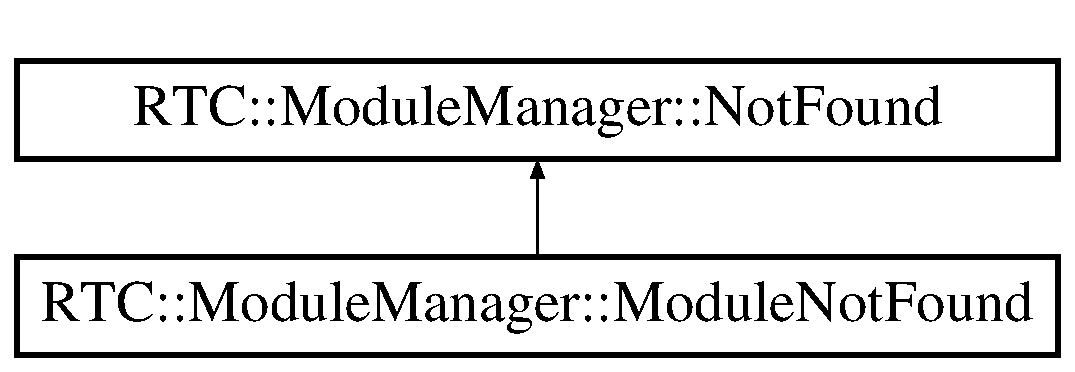
\includegraphics[height=2cm]{structRTC_1_1ModuleManager_1_1ModuleNotFound}
\end{center}
\end{figure}
\subsection*{Public メソッド}
\begin{DoxyCompactItemize}
\item 
{\bf ModuleNotFound} (const std::string \&\_\-name)
\end{DoxyCompactItemize}


\subsection{説明}
指定モジュール不明例外処理用構造体 

\subsection{コンストラクタとデストラクタ}
\index{RTC::ModuleManager::ModuleNotFound@{RTC::ModuleManager::ModuleNotFound}!ModuleNotFound@{ModuleNotFound}}
\index{ModuleNotFound@{ModuleNotFound}!RTC::ModuleManager::ModuleNotFound@{RTC::ModuleManager::ModuleNotFound}}
\subsubsection[{ModuleNotFound}]{\setlength{\rightskip}{0pt plus 5cm}RTC::ModuleManager::ModuleNotFound::ModuleNotFound (const std::string \& {\em \_\-name})\hspace{0.3cm}{\ttfamily  [inline]}}\label{structRTC_1_1ModuleManager_1_1ModuleNotFound_a24f3fd51dff9c8835d5884d1c8e205e5}

\section{クラス RTC::Manager::ModulePredicate}
\label{classRTC_1_1Manager_1_1ModulePredicate}\index{RTC::Manager::ModulePredicate@{RTC::Manager::ModulePredicate}}


{\ttfamily \#include $<$Manager.h$>$}

\subsection*{Public メソッド}
\begin{DoxyCompactItemize}
\item 
{\bf ModulePredicate} ({\bf coil::Properties} \&prop)
\item 
bool {\bf operator()} ({\bf coil::Properties} \&prop)
\end{DoxyCompactItemize}


\subsection{コンストラクタとデストラクタ}
\index{RTC::Manager::ModulePredicate@{RTC::Manager::ModulePredicate}!ModulePredicate@{ModulePredicate}}
\index{ModulePredicate@{ModulePredicate}!RTC::Manager::ModulePredicate@{RTC::Manager::ModulePredicate}}
\subsubsection[{ModulePredicate}]{\setlength{\rightskip}{0pt plus 5cm}RTC::Manager::ModulePredicate::ModulePredicate ({\bf coil::Properties} \& {\em prop})\hspace{0.3cm}{\ttfamily  [inline]}}\label{classRTC_1_1Manager_1_1ModulePredicate_a87f556d3d2b1d8cc0568821c258cad1d}


\subsection{関数}
\index{RTC::Manager::ModulePredicate@{RTC::Manager::ModulePredicate}!operator()@{operator()}}
\index{operator()@{operator()}!RTC::Manager::ModulePredicate@{RTC::Manager::ModulePredicate}}
\subsubsection[{operator()}]{\setlength{\rightskip}{0pt plus 5cm}bool RTC::Manager::ModulePredicate::operator() ({\bf coil::Properties} \& {\em prop})\hspace{0.3cm}{\ttfamily  [inline]}}\label{classRTC_1_1Manager_1_1ModulePredicate_a0ddaada4fc3ed47219fc8bacf7da0aa8}

\section{coil::Mutex Class Reference}
\label{classcoil_1_1Mutex}\index{coil::Mutex@{coil::Mutex}}


\doxyref{Mutex}{p.}{classcoil_1_1Mutex} class.  




{\ttfamily \#include $<$Mutex.h$>$}

\subsection*{Public Member Functions}
\begin{DoxyCompactItemize}
\item 
{\bf Mutex} (const char $\ast$const name=0)
\begin{DoxyCompactList}\small\item\em Constructor. \item\end{DoxyCompactList}\item 
{\bf $\sim$Mutex} ()
\begin{DoxyCompactList}\small\item\em Destructor. \item\end{DoxyCompactList}\item 
void {\bf lock} ()
\begin{DoxyCompactList}\small\item\em Mutual exclusion lock. \item\end{DoxyCompactList}\item 
bool {\bf trylock} ()
\begin{DoxyCompactList}\small\item\em Mutual exclusion non-\/blocking lock. \item\end{DoxyCompactList}\item 
void {\bf unlock} ()
\begin{DoxyCompactList}\small\item\em Mutual exclusion unlock. \item\end{DoxyCompactList}\end{DoxyCompactItemize}
\subsection*{Public Attributes}
\begin{DoxyCompactItemize}
\item 
pthread\_\-mutex\_\-t {\bf mutex\_\-}
\begin{DoxyCompactList}\small\item\em Mutual exclusion object. \item\end{DoxyCompactList}\end{DoxyCompactItemize}


\subsection{Detailed Description}
\doxyref{Mutex}{p.}{classcoil_1_1Mutex} class. 

\subsection{Constructor \& Destructor Documentation}
\index{coil::Mutex@{coil::Mutex}!Mutex@{Mutex}}
\index{Mutex@{Mutex}!coil::Mutex@{coil::Mutex}}
\subsubsection[{Mutex}]{\setlength{\rightskip}{0pt plus 5cm}coil::Mutex::Mutex (const char $\ast$const  {\em name} = {\ttfamily 0})\hspace{0.3cm}{\ttfamily  [inline]}}\label{classcoil_1_1Mutex_a45a1dccbb0d845c4668d832830b3381e}


Constructor. 

Constructor


\begin{DoxyParams}{Parameters}
\item[{\em name}]Object name \end{DoxyParams}


References mutex\_\-.

\index{coil::Mutex@{coil::Mutex}!$\sim$Mutex@{$\sim$Mutex}}
\index{$\sim$Mutex@{$\sim$Mutex}!coil::Mutex@{coil::Mutex}}
\subsubsection[{$\sim$Mutex}]{\setlength{\rightskip}{0pt plus 5cm}coil::Mutex::$\sim$Mutex ()\hspace{0.3cm}{\ttfamily  [inline]}}\label{classcoil_1_1Mutex_ace6ccbe6d64be438633e5fdd33642606}


Destructor. 

Destructor 

References mutex\_\-.



\subsection{Member Function Documentation}
\index{coil::Mutex@{coil::Mutex}!lock@{lock}}
\index{lock@{lock}!coil::Mutex@{coil::Mutex}}
\subsubsection[{lock}]{\setlength{\rightskip}{0pt plus 5cm}void coil::Mutex::lock ()\hspace{0.3cm}{\ttfamily  [inline]}}\label{classcoil_1_1Mutex_abd97daab1969a6cbf0e65ddf9944f669}


Mutual exclusion lock. 

Lock the Mutual exclusion. 

References mutex\_\-.



Referenced by coil::log\_\-stream$<$ \_\-CharT, \_\-Traits $>$::lock().

\index{coil::Mutex@{coil::Mutex}!trylock@{trylock}}
\index{trylock@{trylock}!coil::Mutex@{coil::Mutex}}
\subsubsection[{trylock}]{\setlength{\rightskip}{0pt plus 5cm}bool coil::Mutex::trylock ()\hspace{0.3cm}{\ttfamily  [inline]}}\label{classcoil_1_1Mutex_aaf471565209e694eb5cd308f0c0dabdd}


Mutual exclusion non-\/blocking lock. 

Lock the Mutual exclusion by non-\/blocking. 

References mutex\_\-.

\index{coil::Mutex@{coil::Mutex}!unlock@{unlock}}
\index{unlock@{unlock}!coil::Mutex@{coil::Mutex}}
\subsubsection[{unlock}]{\setlength{\rightskip}{0pt plus 5cm}void coil::Mutex::unlock ()\hspace{0.3cm}{\ttfamily  [inline]}}\label{classcoil_1_1Mutex_aae9502c922762c052edafdeb53aa9baa}


Mutual exclusion unlock. 

Unlock the Mutual exclusion. 

References mutex\_\-.



Referenced by coil::log\_\-stream$<$ \_\-CharT, \_\-Traits $>$::unlock().



\subsection{Member Data Documentation}
\index{coil::Mutex@{coil::Mutex}!mutex\_\-@{mutex\_\-}}
\index{mutex\_\-@{mutex\_\-}!coil::Mutex@{coil::Mutex}}
\subsubsection[{mutex\_\-}]{\setlength{\rightskip}{0pt plus 5cm}pthread\_\-mutex\_\-t {\bf coil::Mutex::mutex\_\-}}\label{classcoil_1_1Mutex_a6ae0f7d95d947ca3a333fc5628225ab7}


Mutual exclusion object. 



Referenced by lock(), Mutex(), trylock(), unlock(), and $\sim$Mutex().


\section{クラス RTC::NamingManager::Names}
\label{classRTC_1_1NamingManager_1_1Names}\index{RTC::NamingManager::Names@{RTC::NamingManager::Names}}


NameServer 管理用構造体.  




{\ttfamily \#include $<$NamingManager.h$>$}

\subsection*{Public メソッド}
\begin{DoxyCompactItemize}
\item 
{\bf Names} (const char $\ast$meth, const char $\ast$name, {\bf NamingBase} $\ast$naming)
\item 
{\bf $\sim$Names} ()
\end{DoxyCompactItemize}
\subsection*{Public 変数}
\begin{DoxyCompactItemize}
\item 
std::string {\bf method}
\item 
std::string {\bf nsname}
\item 
{\bf NamingBase} $\ast$ {\bf ns}
\end{DoxyCompactItemize}


\subsection{説明}
NameServer 管理用構造体. 

\subsection{コンストラクタとデストラクタ}
\index{RTC::NamingManager::Names@{RTC::NamingManager::Names}!Names@{Names}}
\index{Names@{Names}!RTC::NamingManager::Names@{RTC::NamingManager::Names}}
\subsubsection[{Names}]{\setlength{\rightskip}{0pt plus 5cm}RTC::NamingManager::Names::Names (const char $\ast$ {\em meth}, \/  const char $\ast$ {\em name}, \/  {\bf NamingBase} $\ast$ {\em naming})\hspace{0.3cm}{\ttfamily  [inline]}}\label{classRTC_1_1NamingManager_1_1Names_a41f1f4ab7a1312266066594e550105c2}
\index{RTC::NamingManager::Names@{RTC::NamingManager::Names}!$\sim$Names@{$\sim$Names}}
\index{$\sim$Names@{$\sim$Names}!RTC::NamingManager::Names@{RTC::NamingManager::Names}}
\subsubsection[{$\sim$Names}]{\setlength{\rightskip}{0pt plus 5cm}RTC::NamingManager::Names::$\sim$Names ()\hspace{0.3cm}{\ttfamily  [inline]}}\label{classRTC_1_1NamingManager_1_1Names_ac85bbc0dd044798db451ba1b78565088}


\subsection{変数}
\index{RTC::NamingManager::Names@{RTC::NamingManager::Names}!method@{method}}
\index{method@{method}!RTC::NamingManager::Names@{RTC::NamingManager::Names}}
\subsubsection[{method}]{\setlength{\rightskip}{0pt plus 5cm}std::string {\bf RTC::NamingManager::Names::method}}\label{classRTC_1_1NamingManager_1_1Names_af91cd5f33926928072f5f620a83c5ace}
\index{RTC::NamingManager::Names@{RTC::NamingManager::Names}!ns@{ns}}
\index{ns@{ns}!RTC::NamingManager::Names@{RTC::NamingManager::Names}}
\subsubsection[{ns}]{\setlength{\rightskip}{0pt plus 5cm}{\bf NamingBase}$\ast$ {\bf RTC::NamingManager::Names::ns}}\label{classRTC_1_1NamingManager_1_1Names_a704904910fea3bf04cf6db7126ec3c29}
\index{RTC::NamingManager::Names@{RTC::NamingManager::Names}!nsname@{nsname}}
\index{nsname@{nsname}!RTC::NamingManager::Names@{RTC::NamingManager::Names}}
\subsubsection[{nsname}]{\setlength{\rightskip}{0pt plus 5cm}std::string {\bf RTC::NamingManager::Names::nsname}}\label{classRTC_1_1NamingManager_1_1Names_afd60a3c02c75c896ef6110f02acf25b0}

\section{クラス RTC::NamingBase}
\label{classRTC_1_1NamingBase}\index{RTC::NamingBase@{RTC::NamingBase}}


NamingService 管理用抽象クラス.  




{\ttfamily \#include $<$NamingManager.h$>$}

RTC::NamingBaseに対する継承グラフ\begin{figure}[H]
\begin{center}
\leavevmode
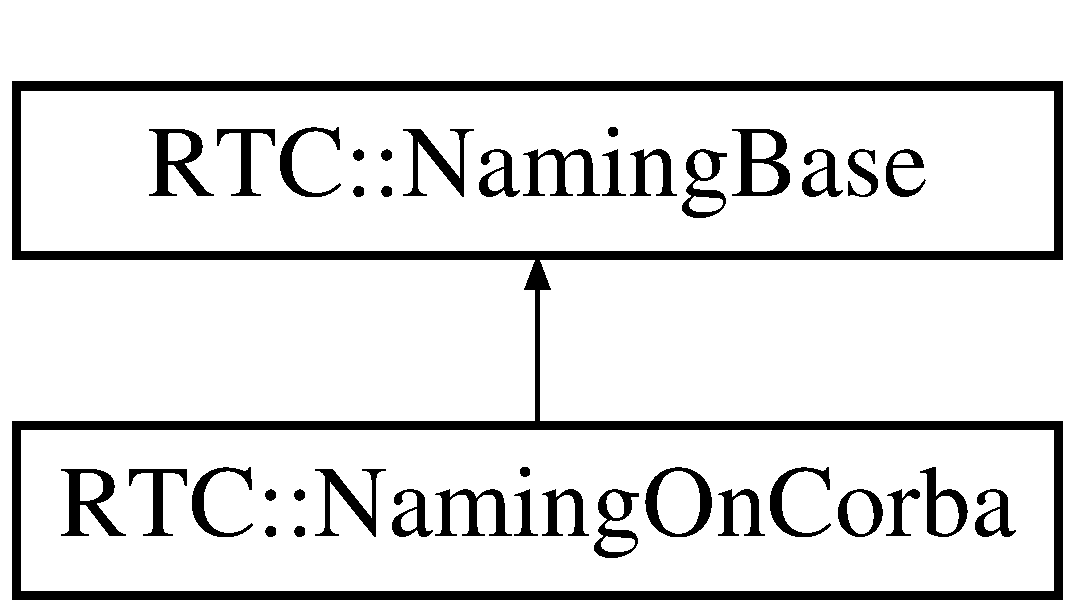
\includegraphics[height=2cm]{classRTC_1_1NamingBase}
\end{center}
\end{figure}
\subsection*{Public メソッド}
\begin{DoxyCompactItemize}
\item 
{\bf NamingBase} ()
\begin{DoxyCompactList}\small\item\em コンストラクタ \item\end{DoxyCompactList}\item 
virtual {\bf $\sim$NamingBase} (void)
\begin{DoxyCompactList}\small\item\em デストラクタ \item\end{DoxyCompactList}\item 
virtual void {\bf bindObject} (const char $\ast$name, const {\bf RTObject\_\-impl} $\ast$rtobj)=0
\begin{DoxyCompactList}\small\item\em 指定したオブジェクトをNamingServiceへバインドする純粋仮想関数 \item\end{DoxyCompactList}\item 
virtual void {\bf bindObject} (const char $\ast$name, const {\bf RTM::ManagerServant} $\ast$mgr)=0
\begin{DoxyCompactList}\small\item\em 指定したManagerServantをNamingServiceへバインドする純粋仮想関数 \item\end{DoxyCompactList}\item 
virtual void {\bf unbindObject} (const char $\ast$name)=0
\begin{DoxyCompactList}\small\item\em 指定したオブジェクトをNamingServiceからアンバインドするための 純粋仮想関数 \item\end{DoxyCompactList}\item 
virtual bool {\bf isAlive} ()=0
\begin{DoxyCompactList}\small\item\em ネームサーバの生存を確認する。 \item\end{DoxyCompactList}\end{DoxyCompactItemize}


\subsection{説明}
NamingService 管理用抽象クラス. NamingServer 管理用抽象インターフェースクラス。 具象管理クラスは、以下の純粋仮想関数の実装を提供しなければならない。
\begin{DoxyItemize}
\item \doxyref{bindObject()}{p.}{classRTC_1_1NamingBase_ac8b6c5670ae869ba80b9407169cc7928} : 指定したオブジェクトのNamingServiceへのバインド
\item \doxyref{unbindObject()}{p.}{classRTC_1_1NamingBase_a78700b13ec16ffadfc80c13461db3832} : 指定したオブジェクトのNamingServiceからのアンバインド
\end{DoxyItemize}

\begin{DoxySince}{から}
0.4.0 
\end{DoxySince}


\subsection{コンストラクタとデストラクタ}
\index{RTC::NamingBase@{RTC::NamingBase}!NamingBase@{NamingBase}}
\index{NamingBase@{NamingBase}!RTC::NamingBase@{RTC::NamingBase}}
\subsubsection[{NamingBase}]{\setlength{\rightskip}{0pt plus 5cm}RTC::NamingBase::NamingBase ()\hspace{0.3cm}{\ttfamily  [inline]}}\label{classRTC_1_1NamingBase_aac7efb11bd9fdddd23b290c655141133}


コンストラクタ 

\index{RTC::NamingBase@{RTC::NamingBase}!$\sim$NamingBase@{$\sim$NamingBase}}
\index{$\sim$NamingBase@{$\sim$NamingBase}!RTC::NamingBase@{RTC::NamingBase}}
\subsubsection[{$\sim$NamingBase}]{\setlength{\rightskip}{0pt plus 5cm}virtual RTC::NamingBase::$\sim$NamingBase (void)\hspace{0.3cm}{\ttfamily  [inline, virtual]}}\label{classRTC_1_1NamingBase_af6d06310a58dd4c8ca09daf727881e26}


デストラクタ 



\subsection{関数}
\index{RTC::NamingBase@{RTC::NamingBase}!bindObject@{bindObject}}
\index{bindObject@{bindObject}!RTC::NamingBase@{RTC::NamingBase}}
\subsubsection[{bindObject}]{\setlength{\rightskip}{0pt plus 5cm}virtual void RTC::NamingBase::bindObject (const char $\ast$ {\em name}, \/  const {\bf RTM::ManagerServant} $\ast$ {\em mgr})\hspace{0.3cm}{\ttfamily  [pure virtual]}}\label{classRTC_1_1NamingBase_a46494e91f57881e0b19faad01f7ea675}


指定したManagerServantをNamingServiceへバインドする純粋仮想関数 


\begin{DoxyParams}{引数}
\item[{\em name}]バインド時の名称 \item[{\em rtobj}]バインド対象ManagerServant \end{DoxyParams}


{\bf RTC::NamingOnCorba} \doxyref{}{p.}{classRTC_1_1NamingOnCorba_a539b34abf7968f2ad2c2a8af46bfe509}で実装されています。

\index{RTC::NamingBase@{RTC::NamingBase}!bindObject@{bindObject}}
\index{bindObject@{bindObject}!RTC::NamingBase@{RTC::NamingBase}}
\subsubsection[{bindObject}]{\setlength{\rightskip}{0pt plus 5cm}virtual void RTC::NamingBase::bindObject (const char $\ast$ {\em name}, \/  const {\bf RTObject\_\-impl} $\ast$ {\em rtobj})\hspace{0.3cm}{\ttfamily  [pure virtual]}}\label{classRTC_1_1NamingBase_ac8b6c5670ae869ba80b9407169cc7928}


指定したオブジェクトをNamingServiceへバインドする純粋仮想関数 


\begin{DoxyParams}{引数}
\item[{\em name}]バインド時の名称 \item[{\em rtobj}]バインド対象オブジェクト \end{DoxyParams}


{\bf RTC::NamingOnCorba} \doxyref{}{p.}{classRTC_1_1NamingOnCorba_a6361ae7eac2cf8788bbc0ad98b4440b3}で実装されています。

\index{RTC::NamingBase@{RTC::NamingBase}!isAlive@{isAlive}}
\index{isAlive@{isAlive}!RTC::NamingBase@{RTC::NamingBase}}
\subsubsection[{isAlive}]{\setlength{\rightskip}{0pt plus 5cm}virtual bool RTC::NamingBase::isAlive ()\hspace{0.3cm}{\ttfamily  [pure virtual]}}\label{classRTC_1_1NamingBase_af2e5abca5e0f91fb1ed6f830b1837318}


ネームサーバの生存を確認する。 

\begin{DoxyReturn}{戻り値}
true:生存している, false:生存していない 
\end{DoxyReturn}


{\bf RTC::NamingOnCorba} \doxyref{}{p.}{classRTC_1_1NamingOnCorba_af48e8a29fce37cb045a14ea452c4031d}で実装されています。

\index{RTC::NamingBase@{RTC::NamingBase}!unbindObject@{unbindObject}}
\index{unbindObject@{unbindObject}!RTC::NamingBase@{RTC::NamingBase}}
\subsubsection[{unbindObject}]{\setlength{\rightskip}{0pt plus 5cm}virtual void RTC::NamingBase::unbindObject (const char $\ast$ {\em name})\hspace{0.3cm}{\ttfamily  [pure virtual]}}\label{classRTC_1_1NamingBase_a78700b13ec16ffadfc80c13461db3832}


指定したオブジェクトをNamingServiceからアンバインドするための 純粋仮想関数 


\begin{DoxyParams}{引数}
\item[{\em name}]アンバインド対象オブジェクト \end{DoxyParams}


{\bf RTC::NamingOnCorba} \doxyref{}{p.}{classRTC_1_1NamingOnCorba_ac9f33dd6f2f4df81640d720057da98da}で実装されています。


\section{クラス RTC::NamingManager}
\label{classRTC_1_1NamingManager}\index{RTC::NamingManager@{RTC::NamingManager}}


NamingServer 管理クラス.  




{\ttfamily \#include $<$NamingManager.h$>$}

\subsection*{構成}
\begin{DoxyCompactItemize}
\item 
struct {\bf Comps}
\begin{DoxyCompactList}\small\item\em コンポーネント管理用構造体 \item\end{DoxyCompactList}\item 
struct {\bf Mgr}
\begin{DoxyCompactList}\small\item\em ManagerServant管理用構造体. \item\end{DoxyCompactList}\item 
class {\bf Names}
\begin{DoxyCompactList}\small\item\em NameServer 管理用構造体. \item\end{DoxyCompactList}\end{DoxyCompactItemize}
\subsection*{Public メソッド}
\begin{DoxyCompactItemize}
\item 
{\bf NamingManager} ({\bf Manager} $\ast$manager)
\begin{DoxyCompactList}\small\item\em コンストラクタ \item\end{DoxyCompactList}\item 
virtual {\bf $\sim$NamingManager} (void)
\begin{DoxyCompactList}\small\item\em デストラクタ \item\end{DoxyCompactList}\item 
void {\bf registerNameServer} (const char $\ast$method, const char $\ast$name\_\-server)
\begin{DoxyCompactList}\small\item\em NameServer の登録. \item\end{DoxyCompactList}\item 
void {\bf bindObject} (const char $\ast$name, const {\bf RTObject\_\-impl} $\ast$rtobj)
\begin{DoxyCompactList}\small\item\em 指定したオブジェクトのNamingServiceへバインド \item\end{DoxyCompactList}\item 
void {\bf bindObject} (const char $\ast$name, const {\bf RTM::ManagerServant} $\ast$mgr)
\begin{DoxyCompactList}\small\item\em 指定したManagerServantのNamingServiceへバインド \item\end{DoxyCompactList}\item 
void {\bf update} ()
\begin{DoxyCompactList}\small\item\em NamingServer の情報の更新. \item\end{DoxyCompactList}\item 
void {\bf unbindObject} (const char $\ast$name)
\begin{DoxyCompactList}\small\item\em 指定したオブジェクトをNamingServiceからアンバインド \item\end{DoxyCompactList}\item 
void {\bf unbindAll} ()
\begin{DoxyCompactList}\small\item\em 全てのオブジェクトをNamingServiceからアンバインド \item\end{DoxyCompactList}\item 
std::vector$<$ {\bf RTObject\_\-impl} $\ast$ $>$ {\bf getObjects} ()
\begin{DoxyCompactList}\small\item\em バインドされている全てのオブジェクトを取得 \item\end{DoxyCompactList}\end{DoxyCompactItemize}
\subsection*{Protected メソッド}
\begin{DoxyCompactItemize}
\item 
{\bf NamingBase} $\ast$ {\bf createNamingObj} (const char $\ast$method, const char $\ast$name\_\-server)
\begin{DoxyCompactList}\small\item\em NameServer 管理用オブジェクトの生成. \item\end{DoxyCompactList}\item 
void {\bf bindCompsTo} ({\bf NamingBase} $\ast$ns)
\begin{DoxyCompactList}\small\item\em 設定済みコンポーネントを NameServer に登録 \item\end{DoxyCompactList}\item 
void {\bf registerCompName} (const char $\ast$name, const {\bf RTObject\_\-impl} $\ast$rtobj)
\begin{DoxyCompactList}\small\item\em NameServer に登録するコンポーネントの設定. \item\end{DoxyCompactList}\item 
void {\bf registerMgrName} (const char $\ast$name, const {\bf RTM::ManagerServant} $\ast$mgr)
\begin{DoxyCompactList}\small\item\em NameServer に登録するManagerServantの設定. \item\end{DoxyCompactList}\item 
void {\bf unregisterCompName} (const char $\ast$name)
\begin{DoxyCompactList}\small\item\em NameServer に登録するコンポーネントの設定解除. \item\end{DoxyCompactList}\item 
void {\bf unregisterMgrName} (const char $\ast$name)
\begin{DoxyCompactList}\small\item\em NameServer に登録するManagerServantの設定解除. \item\end{DoxyCompactList}\item 
void {\bf retryConnection} ({\bf Names} $\ast$ns)
\end{DoxyCompactItemize}
\subsection*{Protected 変数}
\begin{DoxyCompactItemize}
\item 
std::vector$<$ {\bf Names} $\ast$ $>$ {\bf m\_\-names}
\begin{DoxyCompactList}\small\item\em NameServer リスト. \item\end{DoxyCompactList}\item 
{\bf Mutex} {\bf m\_\-namesMutex}
\begin{DoxyCompactList}\small\item\em NameServer リストのmutex. \item\end{DoxyCompactList}\item 
std::vector$<$ {\bf Comps} $\ast$ $>$ {\bf m\_\-compNames}
\begin{DoxyCompactList}\small\item\em コンポーネントリスト \item\end{DoxyCompactList}\item 
{\bf Mutex} {\bf m\_\-compNamesMutex}
\begin{DoxyCompactList}\small\item\em コンポーネントリストのmutex \item\end{DoxyCompactList}\item 
std::vector$<$ {\bf Mgr} $\ast$ $>$ {\bf m\_\-mgrNames}
\begin{DoxyCompactList}\small\item\em ManagerServantリスト. \item\end{DoxyCompactList}\item 
{\bf Mutex} {\bf m\_\-mgrNamesMutex}
\begin{DoxyCompactList}\small\item\em ManagerServantリストのmutex. \item\end{DoxyCompactList}\item 
{\bf Manager} $\ast$ {\bf m\_\-manager}
\begin{DoxyCompactList}\small\item\em マネージャオブジェクト \item\end{DoxyCompactList}\item 
{\bf Logger} {\bf rtclog}
\begin{DoxyCompactList}\small\item\em ロガーストリーム \item\end{DoxyCompactList}\end{DoxyCompactItemize}


\subsection{説明}
NamingServer 管理クラス. NamingServer 管理用クラス。 コンポーネントのNamingServiceへの登録、解除などを管理する。

\begin{DoxySince}{から}
0.4.0 
\end{DoxySince}


\subsection{コンストラクタとデストラクタ}
\index{RTC::NamingManager@{RTC::NamingManager}!NamingManager@{NamingManager}}
\index{NamingManager@{NamingManager}!RTC::NamingManager@{RTC::NamingManager}}
\subsubsection[{NamingManager}]{\setlength{\rightskip}{0pt plus 5cm}RTC::NamingManager::NamingManager ({\bf Manager} $\ast$ {\em manager})}\label{classRTC_1_1NamingManager_a2d927cb41678fb5f21335515340d2c86}


コンストラクタ 

コンストラクタ


\begin{DoxyParams}{引数}
\item[{\em manager}]マネージャオブジェクト \end{DoxyParams}
\index{RTC::NamingManager@{RTC::NamingManager}!$\sim$NamingManager@{$\sim$NamingManager}}
\index{$\sim$NamingManager@{$\sim$NamingManager}!RTC::NamingManager@{RTC::NamingManager}}
\subsubsection[{$\sim$NamingManager}]{\setlength{\rightskip}{0pt plus 5cm}virtual RTC::NamingManager::$\sim$NamingManager (void)\hspace{0.3cm}{\ttfamily  [virtual]}}\label{classRTC_1_1NamingManager_ab8aede9161f52b474eb9ce4a0cfc0bcb}


デストラクタ 



\subsection{関数}
\index{RTC::NamingManager@{RTC::NamingManager}!bindCompsTo@{bindCompsTo}}
\index{bindCompsTo@{bindCompsTo}!RTC::NamingManager@{RTC::NamingManager}}
\subsubsection[{bindCompsTo}]{\setlength{\rightskip}{0pt plus 5cm}void RTC::NamingManager::bindCompsTo ({\bf NamingBase} $\ast$ {\em ns})\hspace{0.3cm}{\ttfamily  [protected]}}\label{classRTC_1_1NamingManager_a7f48ebff1a98fa1e6dc30f34f6f56337}


設定済みコンポーネントを NameServer に登録 

設定済みコンポーネントを指定した NameServer に登録する。


\begin{DoxyParams}{引数}
\item[{\em ns}]登録対象 NameServer \end{DoxyParams}
\index{RTC::NamingManager@{RTC::NamingManager}!bindObject@{bindObject}}
\index{bindObject@{bindObject}!RTC::NamingManager@{RTC::NamingManager}}
\subsubsection[{bindObject}]{\setlength{\rightskip}{0pt plus 5cm}void RTC::NamingManager::bindObject (const char $\ast$ {\em name}, \/  const {\bf RTM::ManagerServant} $\ast$ {\em mgr})}\label{classRTC_1_1NamingManager_ae909f8abcff48157d70f5430a04f5cc1}


指定したManagerServantのNamingServiceへバインド 

指定したManagerServantを指定した名称で CORBA NamingService へバ インドする。


\begin{DoxyParams}{引数}
\item[{\em name}]バインド時の名称 \item[{\em mgr}]バインド対象ManagerServant \end{DoxyParams}
\index{RTC::NamingManager@{RTC::NamingManager}!bindObject@{bindObject}}
\index{bindObject@{bindObject}!RTC::NamingManager@{RTC::NamingManager}}
\subsubsection[{bindObject}]{\setlength{\rightskip}{0pt plus 5cm}void RTC::NamingManager::bindObject (const char $\ast$ {\em name}, \/  const {\bf RTObject\_\-impl} $\ast$ {\em rtobj})}\label{classRTC_1_1NamingManager_ade403b12d90cb607df901d97c3d3c32f}


指定したオブジェクトのNamingServiceへバインド 

指定したオブジェクトを指定した名称で CORBA NamingService へバイ ンドする。


\begin{DoxyParams}{引数}
\item[{\em name}]バインド時の名称 \item[{\em rtobj}]バインド対象オブジェクト \end{DoxyParams}
\index{RTC::NamingManager@{RTC::NamingManager}!createNamingObj@{createNamingObj}}
\index{createNamingObj@{createNamingObj}!RTC::NamingManager@{RTC::NamingManager}}
\subsubsection[{createNamingObj}]{\setlength{\rightskip}{0pt plus 5cm}{\bf NamingBase}$\ast$ RTC::NamingManager::createNamingObj (const char $\ast$ {\em method}, \/  const char $\ast$ {\em name\_\-server})\hspace{0.3cm}{\ttfamily  [protected]}}\label{classRTC_1_1NamingManager_a3c337a0f68c16203eb911d009b190a5a}


NameServer 管理用オブジェクトの生成. 

指定した型のNameServer 管理用オブジェクトを生成する。


\begin{DoxyParams}{引数}
\item[{\em method}]NamingService 形式 \item[{\em name\_\-server}]NameServer 名称\end{DoxyParams}
\begin{DoxyReturn}{戻り値}
生成した NameServer オブジェクト 
\end{DoxyReturn}
\index{RTC::NamingManager@{RTC::NamingManager}!getObjects@{getObjects}}
\index{getObjects@{getObjects}!RTC::NamingManager@{RTC::NamingManager}}
\subsubsection[{getObjects}]{\setlength{\rightskip}{0pt plus 5cm}std::vector$<${\bf RTObject\_\-impl}$\ast$$>$ RTC::NamingManager::getObjects ()}\label{classRTC_1_1NamingManager_a01f71c35884ad26284094de49b504dd0}


バインドされている全てのオブジェクトを取得 

バインドされている全てのオブジェクトを 取得する。

\begin{DoxyReturn}{戻り値}
バインド済みオブジェクト リスト 
\end{DoxyReturn}
\index{RTC::NamingManager@{RTC::NamingManager}!registerCompName@{registerCompName}}
\index{registerCompName@{registerCompName}!RTC::NamingManager@{RTC::NamingManager}}
\subsubsection[{registerCompName}]{\setlength{\rightskip}{0pt plus 5cm}void RTC::NamingManager::registerCompName (const char $\ast$ {\em name}, \/  const {\bf RTObject\_\-impl} $\ast$ {\em rtobj})\hspace{0.3cm}{\ttfamily  [protected]}}\label{classRTC_1_1NamingManager_a35243abca48730805b8172181b7e1256}


NameServer に登録するコンポーネントの設定. 

NameServer に登録するコンポーネントを設定する。


\begin{DoxyParams}{引数}
\item[{\em name}]コンポーネントの登録時名称 \item[{\em rtobj}]登録対象オブジェクト \end{DoxyParams}
\index{RTC::NamingManager@{RTC::NamingManager}!registerMgrName@{registerMgrName}}
\index{registerMgrName@{registerMgrName}!RTC::NamingManager@{RTC::NamingManager}}
\subsubsection[{registerMgrName}]{\setlength{\rightskip}{0pt plus 5cm}void RTC::NamingManager::registerMgrName (const char $\ast$ {\em name}, \/  const {\bf RTM::ManagerServant} $\ast$ {\em mgr})\hspace{0.3cm}{\ttfamily  [protected]}}\label{classRTC_1_1NamingManager_a5980b779fee33d57b28e6d67b897f033}


NameServer に登録するManagerServantの設定. 

NameServer に登録するManagerServantを設定する。


\begin{DoxyParams}{引数}
\item[{\em name}]ManagerServantの登録時名称 \item[{\em mgr}]登録対象ManagerServant \end{DoxyParams}
\index{RTC::NamingManager@{RTC::NamingManager}!registerNameServer@{registerNameServer}}
\index{registerNameServer@{registerNameServer}!RTC::NamingManager@{RTC::NamingManager}}
\subsubsection[{registerNameServer}]{\setlength{\rightskip}{0pt plus 5cm}void RTC::NamingManager::registerNameServer (const char $\ast$ {\em method}, \/  const char $\ast$ {\em name\_\-server})}\label{classRTC_1_1NamingManager_ab2155792df34d57d0ef6a802914bb9e4}


NameServer の登録. 

指定した形式の NameServer を登録する。 現在指定可能な形式は CORBA のみ。


\begin{DoxyParams}{引数}
\item[{\em method}]NamingService の形式 \item[{\em name\_\-server}]登録する NameServer の名称 \end{DoxyParams}
\index{RTC::NamingManager@{RTC::NamingManager}!retryConnection@{retryConnection}}
\index{retryConnection@{retryConnection}!RTC::NamingManager@{RTC::NamingManager}}
\subsubsection[{retryConnection}]{\setlength{\rightskip}{0pt plus 5cm}void RTC::NamingManager::retryConnection ({\bf Names} $\ast$ {\em ns})\hspace{0.3cm}{\ttfamily  [protected]}}\label{classRTC_1_1NamingManager_afd3abcbc1eb01392b58f9f0b2c160736}
\index{RTC::NamingManager@{RTC::NamingManager}!unbindAll@{unbindAll}}
\index{unbindAll@{unbindAll}!RTC::NamingManager@{RTC::NamingManager}}
\subsubsection[{unbindAll}]{\setlength{\rightskip}{0pt plus 5cm}void RTC::NamingManager::unbindAll ()}\label{classRTC_1_1NamingManager_ade0902fd897f9b4e8c37a2f6fba8d76c}


全てのオブジェクトをNamingServiceからアンバインド 

全てのオブジェクトを CORBA NamingService からアンバインドする。 \index{RTC::NamingManager@{RTC::NamingManager}!unbindObject@{unbindObject}}
\index{unbindObject@{unbindObject}!RTC::NamingManager@{RTC::NamingManager}}
\subsubsection[{unbindObject}]{\setlength{\rightskip}{0pt plus 5cm}void RTC::NamingManager::unbindObject (const char $\ast$ {\em name})}\label{classRTC_1_1NamingManager_a3fcfc7666a199f3fd89529a1bc8df3da}


指定したオブジェクトをNamingServiceからアンバインド 

指定したオブジェクトを NamingService からアンバインドする。


\begin{DoxyParams}{引数}
\item[{\em name}]アンバインド対象オブジェクト \end{DoxyParams}
\index{RTC::NamingManager@{RTC::NamingManager}!unregisterCompName@{unregisterCompName}}
\index{unregisterCompName@{unregisterCompName}!RTC::NamingManager@{RTC::NamingManager}}
\subsubsection[{unregisterCompName}]{\setlength{\rightskip}{0pt plus 5cm}void RTC::NamingManager::unregisterCompName (const char $\ast$ {\em name})\hspace{0.3cm}{\ttfamily  [protected]}}\label{classRTC_1_1NamingManager_a038eb214ba1b7a928aa278252ca0f0fb}


NameServer に登録するコンポーネントの設定解除. 

NameServer に登録するコンポーネントの設定を解除する。


\begin{DoxyParams}{引数}
\item[{\em name}]設定解除対象コンポーネントの名称 \end{DoxyParams}
\index{RTC::NamingManager@{RTC::NamingManager}!unregisterMgrName@{unregisterMgrName}}
\index{unregisterMgrName@{unregisterMgrName}!RTC::NamingManager@{RTC::NamingManager}}
\subsubsection[{unregisterMgrName}]{\setlength{\rightskip}{0pt plus 5cm}void RTC::NamingManager::unregisterMgrName (const char $\ast$ {\em name})\hspace{0.3cm}{\ttfamily  [protected]}}\label{classRTC_1_1NamingManager_a95d0916eda2bc1d3f7599696cf9c0485}


NameServer に登録するManagerServantの設定解除. 

NameServer に登録するManagerServantの設定を解除する。


\begin{DoxyParams}{引数}
\item[{\em name}]設定解除対象ManagerServantの名称 \end{DoxyParams}
\index{RTC::NamingManager@{RTC::NamingManager}!update@{update}}
\index{update@{update}!RTC::NamingManager@{RTC::NamingManager}}
\subsubsection[{update}]{\setlength{\rightskip}{0pt plus 5cm}void RTC::NamingManager::update ()}\label{classRTC_1_1NamingManager_a0c71e845495a5eac4e53adb2bf5ae8ec}


NamingServer の情報の更新. 

設定されている NameServer 内に登録されているオブジェクトの情報を 更新する。 

\subsection{変数}
\index{RTC::NamingManager@{RTC::NamingManager}!m\_\-compNames@{m\_\-compNames}}
\index{m\_\-compNames@{m\_\-compNames}!RTC::NamingManager@{RTC::NamingManager}}
\subsubsection[{m\_\-compNames}]{\setlength{\rightskip}{0pt plus 5cm}std::vector$<${\bf Comps}$\ast$$>$ {\bf RTC::NamingManager::m\_\-compNames}\hspace{0.3cm}{\ttfamily  [protected]}}\label{classRTC_1_1NamingManager_a13c4cf95f0fbc44f1686f526a0cf2fde}


コンポーネントリスト 

\index{RTC::NamingManager@{RTC::NamingManager}!m\_\-compNamesMutex@{m\_\-compNamesMutex}}
\index{m\_\-compNamesMutex@{m\_\-compNamesMutex}!RTC::NamingManager@{RTC::NamingManager}}
\subsubsection[{m\_\-compNamesMutex}]{\setlength{\rightskip}{0pt plus 5cm}{\bf Mutex} {\bf RTC::NamingManager::m\_\-compNamesMutex}\hspace{0.3cm}{\ttfamily  [protected]}}\label{classRTC_1_1NamingManager_a6e116477ec6b544f62f8ca212c00080c}


コンポーネントリストのmutex 

\index{RTC::NamingManager@{RTC::NamingManager}!m\_\-manager@{m\_\-manager}}
\index{m\_\-manager@{m\_\-manager}!RTC::NamingManager@{RTC::NamingManager}}
\subsubsection[{m\_\-manager}]{\setlength{\rightskip}{0pt plus 5cm}{\bf Manager}$\ast$ {\bf RTC::NamingManager::m\_\-manager}\hspace{0.3cm}{\ttfamily  [protected]}}\label{classRTC_1_1NamingManager_ab2c3030a11d9ffc21ab657cc5460b627}


マネージャオブジェクト 

\index{RTC::NamingManager@{RTC::NamingManager}!m\_\-mgrNames@{m\_\-mgrNames}}
\index{m\_\-mgrNames@{m\_\-mgrNames}!RTC::NamingManager@{RTC::NamingManager}}
\subsubsection[{m\_\-mgrNames}]{\setlength{\rightskip}{0pt plus 5cm}std::vector$<${\bf Mgr}$\ast$$>$ {\bf RTC::NamingManager::m\_\-mgrNames}\hspace{0.3cm}{\ttfamily  [protected]}}\label{classRTC_1_1NamingManager_ad7df7a9f7c40fd460fd64541c1212bf5}


ManagerServantリスト. 

\index{RTC::NamingManager@{RTC::NamingManager}!m\_\-mgrNamesMutex@{m\_\-mgrNamesMutex}}
\index{m\_\-mgrNamesMutex@{m\_\-mgrNamesMutex}!RTC::NamingManager@{RTC::NamingManager}}
\subsubsection[{m\_\-mgrNamesMutex}]{\setlength{\rightskip}{0pt plus 5cm}{\bf Mutex} {\bf RTC::NamingManager::m\_\-mgrNamesMutex}\hspace{0.3cm}{\ttfamily  [protected]}}\label{classRTC_1_1NamingManager_ad3482ce8bd9129963388cabc0ec82fe9}


ManagerServantリストのmutex. 

\index{RTC::NamingManager@{RTC::NamingManager}!m\_\-names@{m\_\-names}}
\index{m\_\-names@{m\_\-names}!RTC::NamingManager@{RTC::NamingManager}}
\subsubsection[{m\_\-names}]{\setlength{\rightskip}{0pt plus 5cm}std::vector$<${\bf Names}$\ast$$>$ {\bf RTC::NamingManager::m\_\-names}\hspace{0.3cm}{\ttfamily  [protected]}}\label{classRTC_1_1NamingManager_a3ad836712c9cc68d42d3c27181693113}


NameServer リスト. 

\index{RTC::NamingManager@{RTC::NamingManager}!m\_\-namesMutex@{m\_\-namesMutex}}
\index{m\_\-namesMutex@{m\_\-namesMutex}!RTC::NamingManager@{RTC::NamingManager}}
\subsubsection[{m\_\-namesMutex}]{\setlength{\rightskip}{0pt plus 5cm}{\bf Mutex} {\bf RTC::NamingManager::m\_\-namesMutex}\hspace{0.3cm}{\ttfamily  [protected]}}\label{classRTC_1_1NamingManager_a08e0b0067867d2d7ace6bcd655b0c1d3}


NameServer リストのmutex. 

\index{RTC::NamingManager@{RTC::NamingManager}!rtclog@{rtclog}}
\index{rtclog@{rtclog}!RTC::NamingManager@{RTC::NamingManager}}
\subsubsection[{rtclog}]{\setlength{\rightskip}{0pt plus 5cm}{\bf Logger} {\bf RTC::NamingManager::rtclog}\hspace{0.3cm}{\ttfamily  [protected]}}\label{classRTC_1_1NamingManager_a7c15bb6f509227e231bc4f4116b8cf91}


ロガーストリーム 


\section{クラス RTC::NamingOnCorba}
\label{classRTC_1_1NamingOnCorba}\index{RTC::NamingOnCorba@{RTC::NamingOnCorba}}


CORBA 用 NamingServer 管理クラス.  




{\ttfamily \#include $<$NamingManager.h$>$}

RTC::NamingOnCorbaに対する継承グラフ\begin{figure}[H]
\begin{center}
\leavevmode
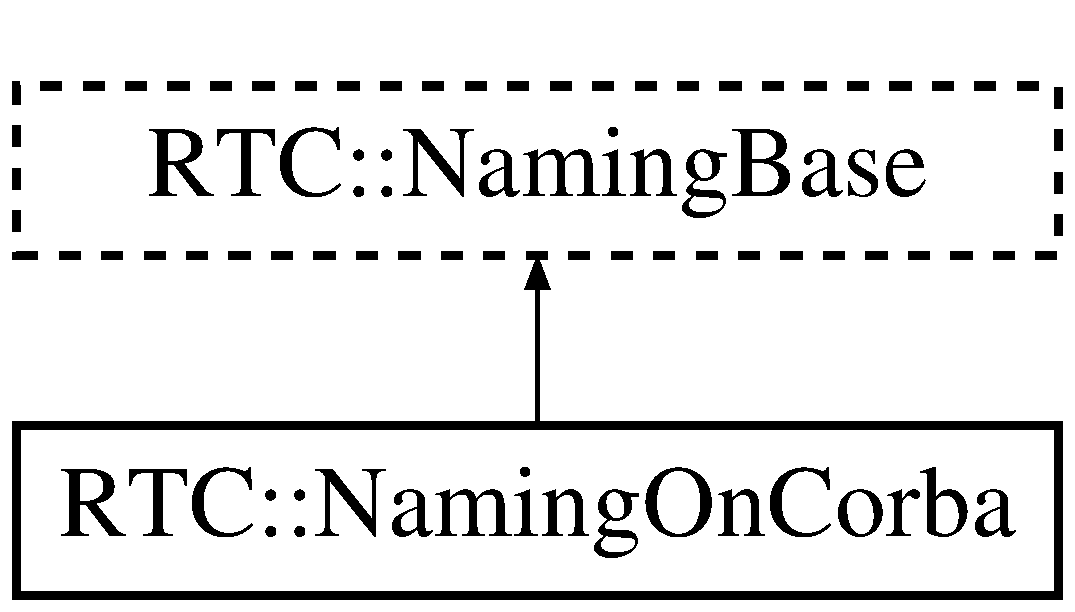
\includegraphics[height=2cm]{classRTC_1_1NamingOnCorba}
\end{center}
\end{figure}
\subsection*{Public メソッド}
\begin{DoxyCompactItemize}
\item 
{\bf NamingOnCorba} (CORBA::ORB\_\-ptr orb, const char $\ast$names)
\begin{DoxyCompactList}\small\item\em コンストラクタ \item\end{DoxyCompactList}\item 
virtual {\bf $\sim$NamingOnCorba} (void)
\begin{DoxyCompactList}\small\item\em デストラクタ \item\end{DoxyCompactList}\item 
virtual void {\bf bindObject} (const char $\ast$name, const {\bf RTObject\_\-impl} $\ast$rtobj)
\begin{DoxyCompactList}\small\item\em 指定した CORBA オブジェクトのNamingServiceへバインド \item\end{DoxyCompactList}\item 
virtual void {\bf bindObject} (const char $\ast$name, const {\bf RTM::ManagerServant} $\ast$mgr)
\begin{DoxyCompactList}\small\item\em 指定したManagerServantをNamingServiceへバインド \item\end{DoxyCompactList}\item 
virtual void {\bf unbindObject} (const char $\ast$name)
\begin{DoxyCompactList}\small\item\em 指定した CORBA オブジェクトをNamingServiceからアンバインド \item\end{DoxyCompactList}\item 
virtual bool {\bf isAlive} ()
\begin{DoxyCompactList}\small\item\em ネームサーバの生存を確認する。 \item\end{DoxyCompactList}\end{DoxyCompactItemize}


\subsection{説明}
CORBA 用 NamingServer 管理クラス. CORBA 用 NamingServer 管理用クラス。 CORBA コンポーネントの NamingService への登録、解除などを管理する。

\begin{DoxySince}{から}
0.4.0 
\end{DoxySince}


\subsection{コンストラクタとデストラクタ}
\index{RTC::NamingOnCorba@{RTC::NamingOnCorba}!NamingOnCorba@{NamingOnCorba}}
\index{NamingOnCorba@{NamingOnCorba}!RTC::NamingOnCorba@{RTC::NamingOnCorba}}
\subsubsection[{NamingOnCorba}]{\setlength{\rightskip}{0pt plus 5cm}RTC::NamingOnCorba::NamingOnCorba (CORBA::ORB\_\-ptr {\em orb}, \/  const char $\ast$ {\em names})}\label{classRTC_1_1NamingOnCorba_ad2cbf61138259ef8717839e906ef1b9e}


コンストラクタ 

コンストラクタ。第2引数に与えるネームサービス名は、ネームサービ スのホスト名とポート番号を \char`\"{}:\char`\"{} で区切ったものである。ポート番号 が省略された場合、2809番ポートが使用される。


\begin{DoxyParams}{引数}
\item[{\em orb}]ORB \item[{\em names}]NamingServer 名称 \end{DoxyParams}
\index{RTC::NamingOnCorba@{RTC::NamingOnCorba}!$\sim$NamingOnCorba@{$\sim$NamingOnCorba}}
\index{$\sim$NamingOnCorba@{$\sim$NamingOnCorba}!RTC::NamingOnCorba@{RTC::NamingOnCorba}}
\subsubsection[{$\sim$NamingOnCorba}]{\setlength{\rightskip}{0pt plus 5cm}virtual RTC::NamingOnCorba::$\sim$NamingOnCorba (void)\hspace{0.3cm}{\ttfamily  [inline, virtual]}}\label{classRTC_1_1NamingOnCorba_ad52223d47212b6fc1b1196b0294eb0a9}


デストラクタ 



\subsection{関数}
\index{RTC::NamingOnCorba@{RTC::NamingOnCorba}!bindObject@{bindObject}}
\index{bindObject@{bindObject}!RTC::NamingOnCorba@{RTC::NamingOnCorba}}
\subsubsection[{bindObject}]{\setlength{\rightskip}{0pt plus 5cm}virtual void RTC::NamingOnCorba::bindObject (const char $\ast$ {\em name}, \/  const {\bf RTM::ManagerServant} $\ast$ {\em mgr})\hspace{0.3cm}{\ttfamily  [virtual]}}\label{classRTC_1_1NamingOnCorba_a539b34abf7968f2ad2c2a8af46bfe509}


指定したManagerServantをNamingServiceへバインド 


\begin{DoxyParams}{引数}
\item[{\em name}]バインド時の名称 \item[{\em rtobj}]バインド対象ManagerServant \end{DoxyParams}


{\bf RTC::NamingBase} \doxyref{}{p.}{classRTC_1_1NamingBase_a46494e91f57881e0b19faad01f7ea675}を実装しています。

\index{RTC::NamingOnCorba@{RTC::NamingOnCorba}!bindObject@{bindObject}}
\index{bindObject@{bindObject}!RTC::NamingOnCorba@{RTC::NamingOnCorba}}
\subsubsection[{bindObject}]{\setlength{\rightskip}{0pt plus 5cm}virtual void RTC::NamingOnCorba::bindObject (const char $\ast$ {\em name}, \/  const {\bf RTObject\_\-impl} $\ast$ {\em rtobj})\hspace{0.3cm}{\ttfamily  [virtual]}}\label{classRTC_1_1NamingOnCorba_a6361ae7eac2cf8788bbc0ad98b4440b3}


指定した CORBA オブジェクトのNamingServiceへバインド 

指定した CORBA オブジェクトを指定した名称で CORBA NamingService へ バインドする。


\begin{DoxyParams}{引数}
\item[{\em name}]バインド時の名称 \item[{\em rtobj}]バインド対象オブジェクト \end{DoxyParams}


{\bf RTC::NamingBase} \doxyref{}{p.}{classRTC_1_1NamingBase_ac8b6c5670ae869ba80b9407169cc7928}を実装しています。

\index{RTC::NamingOnCorba@{RTC::NamingOnCorba}!isAlive@{isAlive}}
\index{isAlive@{isAlive}!RTC::NamingOnCorba@{RTC::NamingOnCorba}}
\subsubsection[{isAlive}]{\setlength{\rightskip}{0pt plus 5cm}virtual bool RTC::NamingOnCorba::isAlive ()\hspace{0.3cm}{\ttfamily  [virtual]}}\label{classRTC_1_1NamingOnCorba_af48e8a29fce37cb045a14ea452c4031d}


ネームサーバの生存を確認する。 

\begin{DoxyReturn}{戻り値}
true:生存している, false:生存していない 
\end{DoxyReturn}


{\bf RTC::NamingBase} \doxyref{}{p.}{classRTC_1_1NamingBase_af2e5abca5e0f91fb1ed6f830b1837318}を実装しています。

\index{RTC::NamingOnCorba@{RTC::NamingOnCorba}!unbindObject@{unbindObject}}
\index{unbindObject@{unbindObject}!RTC::NamingOnCorba@{RTC::NamingOnCorba}}
\subsubsection[{unbindObject}]{\setlength{\rightskip}{0pt plus 5cm}virtual void RTC::NamingOnCorba::unbindObject (const char $\ast$ {\em name})\hspace{0.3cm}{\ttfamily  [virtual]}}\label{classRTC_1_1NamingOnCorba_ac9f33dd6f2f4df81640d720057da98da}


指定した CORBA オブジェクトをNamingServiceからアンバインド 

指定した CORBA オブジェクトを CORBA NamingService からアンバインドする。


\begin{DoxyParams}{引数}
\item[{\em name}]アンバインド対象オブジェクト \end{DoxyParams}


{\bf RTC::NamingBase} \doxyref{}{p.}{classRTC_1_1NamingBase_a78700b13ec16ffadfc80c13461db3832}を実装しています。


\section{coil::NonCopyable Class Reference}
\label{classcoil_1_1NonCopyable}\index{coil::NonCopyable@{coil::NonCopyable}}


Non-\/copyable Mixin.  




{\ttfamily \#include $<$NonCopyable.h$>$}

\subsection*{Protected Member Functions}
\begin{DoxyCompactItemize}
\item 
{\bf NonCopyable} ()
\begin{DoxyCompactList}\small\item\em Constructor. \item\end{DoxyCompactList}\item 
{\bf $\sim$NonCopyable} ()
\begin{DoxyCompactList}\small\item\em Destructor. \item\end{DoxyCompactList}\end{DoxyCompactItemize}


\subsection{Detailed Description}
Non-\/copyable Mixin. This mix-\/in class prevents objects of a class from being copy-\/constructed or assigned to each other. User can prohibit the class copying by inheriting from \doxyref{NonCopyable}{p.}{classcoil_1_1NonCopyable} class as a private base class.

-\/example: class CopyProhibitedClass : private \doxyref{NonCopyable}{p.}{classcoil_1_1NonCopyable} \{\};

This mix-\/in class prevents objects of a class from being copy-\/constructed or assigned to each other. User can prohibit the class copying by inheriting from \doxyref{NonCopyable}{p.}{classcoil_1_1NonCopyable} class as a private base class. The CRTP (Curiously Recursive Template Pattern) version would be used for empty base optimization for multipe-\/inherited.

-\/example: class CopyProhibitedClass : private \doxyref{NonCopyable}{p.}{classcoil_1_1NonCopyable} \{\}; 

\subsection{Constructor \& Destructor Documentation}
\index{coil::NonCopyable@{coil::NonCopyable}!NonCopyable@{NonCopyable}}
\index{NonCopyable@{NonCopyable}!coil::NonCopyable@{coil::NonCopyable}}
\subsubsection[{NonCopyable}]{\setlength{\rightskip}{0pt plus 5cm}coil::NonCopyable::NonCopyable ()\hspace{0.3cm}{\ttfamily  [inline, protected]}}\label{classcoil_1_1NonCopyable_a4e2595899e62bfe0ed4db66e285b85d9}


Constructor. 

Constructor \index{coil::NonCopyable@{coil::NonCopyable}!$\sim$NonCopyable@{$\sim$NonCopyable}}
\index{$\sim$NonCopyable@{$\sim$NonCopyable}!coil::NonCopyable@{coil::NonCopyable}}
\subsubsection[{$\sim$NonCopyable}]{\setlength{\rightskip}{0pt plus 5cm}coil::NonCopyable::$\sim$NonCopyable ()\hspace{0.3cm}{\ttfamily  [inline, protected]}}\label{classcoil_1_1NonCopyable_a0dc4a13a68c4f3a35a74378cf949f53a}


Destructor. 

Destructor 
\section{coil::NonCopyableCRTP$<$ T $>$ Class Template Reference}
\label{classcoil_1_1NonCopyableCRTP}\index{coil::NonCopyableCRTP@{coil::NonCopyableCRTP}}


{\ttfamily \#include $<$NonCopyable.h$>$}

\subsection*{Protected Member Functions}
\begin{DoxyCompactItemize}
\item 
{\bf NonCopyableCRTP} ()
\begin{DoxyCompactList}\small\item\em Constructor. \item\end{DoxyCompactList}\item 
{\bf $\sim$NonCopyableCRTP} ()
\begin{DoxyCompactList}\small\item\em Destructor. \item\end{DoxyCompactList}\end{DoxyCompactItemize}
\subsubsection*{template$<$class T$>$ class coil::NonCopyableCRTP$<$ T $>$}



\subsection{Constructor \& Destructor Documentation}
\index{coil::NonCopyableCRTP@{coil::NonCopyableCRTP}!NonCopyableCRTP@{NonCopyableCRTP}}
\index{NonCopyableCRTP@{NonCopyableCRTP}!coil::NonCopyableCRTP@{coil::NonCopyableCRTP}}
\subsubsection[{NonCopyableCRTP}]{\setlength{\rightskip}{0pt plus 5cm}template$<$class T $>$ {\bf coil::NonCopyableCRTP}$<$ T $>$::{\bf NonCopyableCRTP} ()\hspace{0.3cm}{\ttfamily  [inline, protected]}}\label{classcoil_1_1NonCopyableCRTP_a3234df905b8bb0c1fdbff8d86c5d3933}


Constructor. 

Constructor \index{coil::NonCopyableCRTP@{coil::NonCopyableCRTP}!$\sim$NonCopyableCRTP@{$\sim$NonCopyableCRTP}}
\index{$\sim$NonCopyableCRTP@{$\sim$NonCopyableCRTP}!coil::NonCopyableCRTP@{coil::NonCopyableCRTP}}
\subsubsection[{$\sim$NonCopyableCRTP}]{\setlength{\rightskip}{0pt plus 5cm}template$<$class T $>$ {\bf coil::NonCopyableCRTP}$<$ T $>$::$\sim${\bf NonCopyableCRTP} ()\hspace{0.3cm}{\ttfamily  [inline, protected]}}\label{classcoil_1_1NonCopyableCRTP_abf9fdd83a0a9a7d3ea13268ba12c41c6}


Destructor. 

Destructor 
\section{RTC::ModuleManager::NotAllowedOperation Struct Reference}
\label{structRTC_1_1ModuleManager_1_1NotAllowedOperation}\index{RTC::ModuleManager::NotAllowedOperation@{RTC::ModuleManager::NotAllowedOperation}}


Structure for exception handling when specified operation cannot be allowed.  




{\ttfamily \#include $<$ModuleManager.h$>$}

Inheritance diagram for RTC::ModuleManager::NotAllowedOperation:\begin{figure}[H]
\begin{center}
\leavevmode
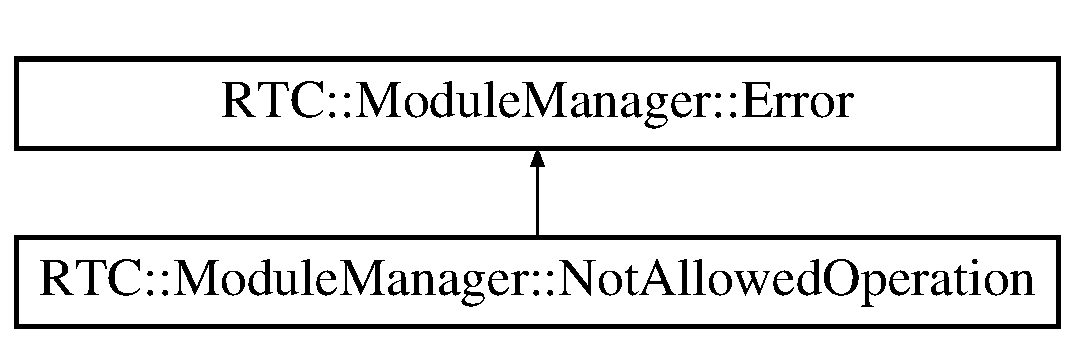
\includegraphics[height=2cm]{structRTC_1_1ModuleManager_1_1NotAllowedOperation}
\end{center}
\end{figure}
\subsection*{Public Member Functions}
\begin{DoxyCompactItemize}
\item 
{\bf NotAllowedOperation} (const std::string \&\_\-reason)
\end{DoxyCompactItemize}


\subsection{Detailed Description}
Structure for exception handling when specified operation cannot be allowed. 

\subsection{Constructor \& Destructor Documentation}
\index{RTC::ModuleManager::NotAllowedOperation@{RTC::ModuleManager::NotAllowedOperation}!NotAllowedOperation@{NotAllowedOperation}}
\index{NotAllowedOperation@{NotAllowedOperation}!RTC::ModuleManager::NotAllowedOperation@{RTC::ModuleManager::NotAllowedOperation}}
\subsubsection[{NotAllowedOperation}]{\setlength{\rightskip}{0pt plus 5cm}RTC::ModuleManager::NotAllowedOperation::NotAllowedOperation (const std::string \& {\em \_\-reason})\hspace{0.3cm}{\ttfamily  [inline]}}\label{structRTC_1_1ModuleManager_1_1NotAllowedOperation_ac7b43e23a013618df637bdd777c90dbc}

\section{構造体 RTC::ModuleManager::NotFound}
\label{structRTC_1_1ModuleManager_1_1NotFound}\index{RTC::ModuleManager::NotFound@{RTC::ModuleManager::NotFound}}


未実装部,指定モジュール不明例外処理用構造体  




{\ttfamily \#include $<$ModuleManager.h$>$}

RTC::ModuleManager::NotFoundに対する継承グラフ\begin{figure}[H]
\begin{center}
\leavevmode
\includegraphics[height=1.51762cm]{structRTC_1_1ModuleManager_1_1NotFound}
\end{center}
\end{figure}
\subsection*{Public メソッド}
\begin{DoxyCompactItemize}
\item 
{\bf NotFound} (const std::string \&\_\-name)
\end{DoxyCompactItemize}
\subsection*{Public 変数}
\begin{DoxyCompactItemize}
\item 
std::string {\bf name}
\end{DoxyCompactItemize}


\subsection{説明}
未実装部,指定モジュール不明例外処理用構造体 

\subsection{コンストラクタとデストラクタ}
\index{RTC::ModuleManager::NotFound@{RTC::ModuleManager::NotFound}!NotFound@{NotFound}}
\index{NotFound@{NotFound}!RTC::ModuleManager::NotFound@{RTC::ModuleManager::NotFound}}
\subsubsection[{NotFound}]{\setlength{\rightskip}{0pt plus 5cm}RTC::ModuleManager::NotFound::NotFound (const std::string \& {\em \_\-name})\hspace{0.3cm}{\ttfamily  [inline]}}\label{structRTC_1_1ModuleManager_1_1NotFound_a70e1590e2ecdedf83a59766290d47650}


\subsection{変数}
\index{RTC::ModuleManager::NotFound@{RTC::ModuleManager::NotFound}!name@{name}}
\index{name@{name}!RTC::ModuleManager::NotFound@{RTC::ModuleManager::NotFound}}
\subsubsection[{name}]{\setlength{\rightskip}{0pt plus 5cm}std::string {\bf RTC::ModuleManager::NotFound::name}}\label{structRTC_1_1ModuleManager_1_1NotFound_a6c1e71e3585e7fe3aa7a3f6905454944}

\section{クラス テンプレート RTC::NullBuffer$<$ DataType $>$}
\label{classRTC_1_1NullBuffer}\index{RTC::NullBuffer@{RTC::NullBuffer}}


ダミーバッファ実装クラス  




{\ttfamily \#include $<$BufferBase.h$>$}

RTC::NullBuffer$<$ DataType $>$に対する継承グラフ\begin{figure}[H]
\begin{center}
\leavevmode
\includegraphics[height=3cm]{classRTC_1_1NullBuffer}
\end{center}
\end{figure}
\subsection*{Public メソッド}
\begin{DoxyCompactItemize}
\item 
{\bf NullBuffer} (long int size=1)
\begin{DoxyCompactList}\small\item\em コンストラクタ \item\end{DoxyCompactList}\item 
virtual {\bf $\sim$NullBuffer} (void)
\begin{DoxyCompactList}\small\item\em デストラクタ \item\end{DoxyCompactList}\item 
virtual long int {\bf length} (void) const 
\begin{DoxyCompactList}\small\item\em バッファ長(1固定)を取得する \item\end{DoxyCompactList}\item 
virtual bool {\bf write} (const DataType \&value)
\begin{DoxyCompactList}\small\item\em バッファにデータを書き込む \item\end{DoxyCompactList}\item 
virtual bool {\bf read} (DataType \&value)
\begin{DoxyCompactList}\small\item\em バッファからデータを読み出す \item\end{DoxyCompactList}\item 
virtual bool {\bf isFull} (void) const 
\begin{DoxyCompactList}\small\item\em バッファfullチェック \item\end{DoxyCompactList}\item 
virtual bool {\bf isEmpty} (void) const 
\begin{DoxyCompactList}\small\item\em バッファemptyチェック \item\end{DoxyCompactList}\end{DoxyCompactItemize}
\subsection*{Protected メソッド}
\begin{DoxyCompactItemize}
\item 
virtual void {\bf put} (const DataType \&data)
\begin{DoxyCompactList}\small\item\em バッファにデータを格納 \item\end{DoxyCompactList}\item 
virtual const DataType \& {\bf get} (void)
\begin{DoxyCompactList}\small\item\em バッファからデータを取得する \item\end{DoxyCompactList}\item 
virtual DataType \& {\bf getRef} (void)
\begin{DoxyCompactList}\small\item\em 次に書き込むバッファへの参照を取得する \item\end{DoxyCompactList}\end{DoxyCompactItemize}


\subsection{説明}
\subsubsection*{template$<$class DataType$>$ class RTC::NullBuffer$<$ DataType $>$}

ダミーバッファ実装クラス バッファ長が1固定のダミーバッファ実装クラス。 $<$DataType$>$としてバッファ内で保持するデータ型を指定する。


\begin{DoxyParams}{引数}
\item[{\em DataType}]バッファに格納するデータ型\end{DoxyParams}
\begin{DoxySince}{から}
0.4.0 
\end{DoxySince}


\subsection{コンストラクタとデストラクタ}
\index{RTC::NullBuffer@{RTC::NullBuffer}!NullBuffer@{NullBuffer}}
\index{NullBuffer@{NullBuffer}!RTC::NullBuffer@{RTC::NullBuffer}}
\subsubsection[{NullBuffer}]{\setlength{\rightskip}{0pt plus 5cm}template$<$class DataType $>$ {\bf RTC::NullBuffer}$<$ DataType $>$::{\bf NullBuffer} (long int {\em size} = {\ttfamily 1})\hspace{0.3cm}{\ttfamily  [inline]}}\label{classRTC_1_1NullBuffer_a77ef32c2911444bcc2cce77c66ae3e00}


コンストラクタ 

コンストラクタ バッファ長を1(固定)で初期化する。


\begin{DoxyParams}{引数}
\item[{\em size}]バッファ長(ただし無効) \end{DoxyParams}
\index{RTC::NullBuffer@{RTC::NullBuffer}!$\sim$NullBuffer@{$\sim$NullBuffer}}
\index{$\sim$NullBuffer@{$\sim$NullBuffer}!RTC::NullBuffer@{RTC::NullBuffer}}
\subsubsection[{$\sim$NullBuffer}]{\setlength{\rightskip}{0pt plus 5cm}template$<$class DataType $>$ virtual {\bf RTC::NullBuffer}$<$ DataType $>$::$\sim${\bf NullBuffer} (void)\hspace{0.3cm}{\ttfamily  [inline, virtual]}}\label{classRTC_1_1NullBuffer_a95ff13580dbab77a497c1838a9bf03c1}


デストラクタ 

デストラクタ。 

\subsection{関数}
\index{RTC::NullBuffer@{RTC::NullBuffer}!get@{get}}
\index{get@{get}!RTC::NullBuffer@{RTC::NullBuffer}}
\subsubsection[{get}]{\setlength{\rightskip}{0pt plus 5cm}template$<$class DataType $>$ virtual const DataType\& {\bf RTC::NullBuffer}$<$ DataType $>$::get (void)\hspace{0.3cm}{\ttfamily  [inline, protected, virtual]}}\label{classRTC_1_1NullBuffer_a5acb245659e61424bda0080b44d7b6d1}


バッファからデータを取得する 

バッファに格納されたデータを取得する。

\begin{DoxyReturn}{戻り値}
取得データ 
\end{DoxyReturn}


{\bf RTC::BufferBase$<$ DataType $>$} \doxyref{}{p.}{classRTC_1_1BufferBase_af12dcf239b3842fe6c946cb61c3d0bd2}を実装しています。

\index{RTC::NullBuffer@{RTC::NullBuffer}!getRef@{getRef}}
\index{getRef@{getRef}!RTC::NullBuffer@{RTC::NullBuffer}}
\subsubsection[{getRef}]{\setlength{\rightskip}{0pt plus 5cm}template$<$class DataType $>$ virtual DataType\& {\bf RTC::NullBuffer}$<$ DataType $>$::getRef (void)\hspace{0.3cm}{\ttfamily  [inline, protected, virtual]}}\label{classRTC_1_1NullBuffer_a5447a6f2d9022baf5394c5afdb4b227e}


次に書き込むバッファへの参照を取得する 

書き込みバッファへの参照を取得する。 本バッファ実装ではバッファ長は固定で1であるため, 常に同じ位置への参照を返す。

\begin{DoxyReturn}{戻り値}
次の書き込み対象バッファへの参照(固定) 
\end{DoxyReturn}
\index{RTC::NullBuffer@{RTC::NullBuffer}!isEmpty@{isEmpty}}
\index{isEmpty@{isEmpty}!RTC::NullBuffer@{RTC::NullBuffer}}
\subsubsection[{isEmpty}]{\setlength{\rightskip}{0pt plus 5cm}template$<$class DataType $>$ virtual bool {\bf RTC::NullBuffer}$<$ DataType $>$::isEmpty (void) const\hspace{0.3cm}{\ttfamily  [inline, virtual]}}\label{classRTC_1_1NullBuffer_a29726dbdb85caaf69229105718f15dc1}


バッファemptyチェック 

バッファemptyをチェックする。(常にfalseを返す。)

\begin{DoxyReturn}{戻り値}
emptyチェック結果(常にfalse) 
\end{DoxyReturn}
\index{RTC::NullBuffer@{RTC::NullBuffer}!isFull@{isFull}}
\index{isFull@{isFull}!RTC::NullBuffer@{RTC::NullBuffer}}
\subsubsection[{isFull}]{\setlength{\rightskip}{0pt plus 5cm}template$<$class DataType $>$ virtual bool {\bf RTC::NullBuffer}$<$ DataType $>$::isFull (void) const\hspace{0.3cm}{\ttfamily  [inline, virtual]}}\label{classRTC_1_1NullBuffer_a32bf047061497e79daded3ce2f558ccb}


バッファfullチェック 

バッファfullをチェックする。(常にfalseを返す。)

\begin{DoxyReturn}{戻り値}
fullチェック結果(常にfalse) 
\end{DoxyReturn}
\index{RTC::NullBuffer@{RTC::NullBuffer}!length@{length}}
\index{length@{length}!RTC::NullBuffer@{RTC::NullBuffer}}
\subsubsection[{length}]{\setlength{\rightskip}{0pt plus 5cm}template$<$class DataType $>$ virtual long int {\bf RTC::NullBuffer}$<$ DataType $>$::length (void) const\hspace{0.3cm}{\ttfamily  [inline, virtual]}}\label{classRTC_1_1NullBuffer_a10b3ecbf48ec0987e321465f21887030}


バッファ長(1固定)を取得する 

バッファ長を取得する。(常に1を返す。)

\begin{DoxyReturn}{戻り値}
バッファ長(1固定) 
\end{DoxyReturn}


{\bf RTC::BufferBase$<$ DataType $>$} \doxyref{}{p.}{classRTC_1_1BufferBase_ad41d5476f9bce0e737115e8ab7cc615f}を実装しています。

\index{RTC::NullBuffer@{RTC::NullBuffer}!put@{put}}
\index{put@{put}!RTC::NullBuffer@{RTC::NullBuffer}}
\subsubsection[{put}]{\setlength{\rightskip}{0pt plus 5cm}template$<$class DataType $>$ virtual void {\bf RTC::NullBuffer}$<$ DataType $>$::put (const DataType \& {\em data})\hspace{0.3cm}{\ttfamily  [inline, protected, virtual]}}\label{classRTC_1_1NullBuffer_a0704a4190bd82c637635528ea4c28416}


バッファにデータを格納 

引数で与えられたデータをバッファに格納する。


\begin{DoxyParams}{引数}
\item[{\em data}]対象データ \end{DoxyParams}


{\bf RTC::BufferBase$<$ DataType $>$} \doxyref{}{p.}{classRTC_1_1BufferBase_af6274c9bc458580643560752f9150235}を実装しています。

\index{RTC::NullBuffer@{RTC::NullBuffer}!read@{read}}
\index{read@{read}!RTC::NullBuffer@{RTC::NullBuffer}}
\subsubsection[{read}]{\setlength{\rightskip}{0pt plus 5cm}template$<$class DataType $>$ virtual bool {\bf RTC::NullBuffer}$<$ DataType $>$::read (DataType \& {\em value})\hspace{0.3cm}{\ttfamily  [inline, virtual]}}\label{classRTC_1_1NullBuffer_a8aca824119c1579a6dceb42a7e5833f7}


バッファからデータを読み出す 

バッファに格納されたデータを読み出す。


\begin{DoxyParams}{引数}
\item[{\em value}]読み出したデータ\end{DoxyParams}
\begin{DoxyReturn}{戻り値}
データ読み出し結果(true:読み出し成功,false:読み出し失敗) 
\end{DoxyReturn}
\index{RTC::NullBuffer@{RTC::NullBuffer}!write@{write}}
\index{write@{write}!RTC::NullBuffer@{RTC::NullBuffer}}
\subsubsection[{write}]{\setlength{\rightskip}{0pt plus 5cm}template$<$class DataType $>$ virtual bool {\bf RTC::NullBuffer}$<$ DataType $>$::write (const DataType \& {\em value})\hspace{0.3cm}{\ttfamily  [inline, virtual]}}\label{classRTC_1_1NullBuffer_aa5b727d115e44544be3a7997a5be2e19}


バッファにデータを書き込む 

引数で与えられたデータをバッファに書き込む。


\begin{DoxyParams}{引数}
\item[{\em value}]書き込み対象データ\end{DoxyParams}
\begin{DoxyReturn}{戻り値}
データ書き込み結果(true:書き込み成功,false:書き込み失敗) 
\end{DoxyReturn}

\section{NumberingPolicy Class Reference}
\label{classNumberingPolicy}\index{NumberingPolicy@{NumberingPolicy}}


Abstruct class for naming policy management when creating objects.  




{\ttfamily \#include $<$NumberingPolicy.h$>$}

Inheritance diagram for NumberingPolicy:\begin{figure}[H]
\begin{center}
\leavevmode
\includegraphics[height=2cm]{classNumberingPolicy}
\end{center}
\end{figure}
\subsection*{Classes}
\begin{DoxyCompactItemize}
\item 
struct {\bf ObjectNotFound}
\begin{DoxyCompactList}\small\item\em The structures for exception handling when object was not found. \item\end{DoxyCompactList}\end{DoxyCompactItemize}
\subsection*{Public Member Functions}
\begin{DoxyCompactItemize}
\item 
virtual {\bf $\sim$NumberingPolicy} (void)
\begin{DoxyCompactList}\small\item\em Virtual destractor. \item\end{DoxyCompactList}\item 
virtual std::string {\bf onCreate} (void $\ast$obj)=0
\begin{DoxyCompactList}\small\item\em Create the name when creating objects. \item\end{DoxyCompactList}\item 
virtual void {\bf onDelete} (void $\ast$obj)=0
\begin{DoxyCompactList}\small\item\em Delete the name when deleting objects. \item\end{DoxyCompactList}\end{DoxyCompactItemize}


\subsection{Detailed Description}
Abstruct class for naming policy management when creating objects. This is the abstract interface class to manage the naming policy when creating objects. Concrete classes must implement the following pure virtual functions.
\begin{DoxyItemize}
\item \doxyref{onCreate()}{p.}{classNumberingPolicy_a5a24d7cdf2cff8c97b1c798114504c31} : Create the name when creating objects.
\item \doxyref{onDelete()}{p.}{classNumberingPolicy_a0bc5ddc2193e6415142327b4a5814d86} : Delete the name when deleting objects.
\end{DoxyItemize}

\begin{DoxySince}{Since}
0.4.0 
\end{DoxySince}


\subsection{Constructor \& Destructor Documentation}
\index{NumberingPolicy@{NumberingPolicy}!$\sim$NumberingPolicy@{$\sim$NumberingPolicy}}
\index{$\sim$NumberingPolicy@{$\sim$NumberingPolicy}!NumberingPolicy@{NumberingPolicy}}
\subsubsection[{$\sim$NumberingPolicy}]{\setlength{\rightskip}{0pt plus 5cm}virtual NumberingPolicy::$\sim$NumberingPolicy (void)\hspace{0.3cm}{\ttfamily  [inline, virtual]}}\label{classNumberingPolicy_a07bd719848068793ca84f4ce87f57db7}


Virtual destractor. 



\subsection{Member Function Documentation}
\index{NumberingPolicy@{NumberingPolicy}!onCreate@{onCreate}}
\index{onCreate@{onCreate}!NumberingPolicy@{NumberingPolicy}}
\subsubsection[{onCreate}]{\setlength{\rightskip}{0pt plus 5cm}virtual std::string NumberingPolicy::onCreate (void $\ast$ {\em obj})\hspace{0.3cm}{\ttfamily  [pure virtual]}}\label{classNumberingPolicy_a5a24d7cdf2cff8c97b1c798114504c31}


Create the name when creating objects. 

Pure virtual function to create the name when creating objects.


\begin{DoxyParams}{Parameters}
\item[{\em obj}]The target object for the creation\end{DoxyParams}
\begin{DoxyReturn}{Returns}
Name of the created object 
\end{DoxyReturn}


Implemented in {\bf DefaultNumberingPolicy} \doxyref{}{p.}{classDefaultNumberingPolicy_ad446abe9c24085dc3676a316e0d5da0c}.

\index{NumberingPolicy@{NumberingPolicy}!onDelete@{onDelete}}
\index{onDelete@{onDelete}!NumberingPolicy@{NumberingPolicy}}
\subsubsection[{onDelete}]{\setlength{\rightskip}{0pt plus 5cm}virtual void NumberingPolicy::onDelete (void $\ast$ {\em obj})\hspace{0.3cm}{\ttfamily  [pure virtual]}}\label{classNumberingPolicy_a0bc5ddc2193e6415142327b4a5814d86}


Delete the name when deleting objects. 

Pure virtual function to delete the name when deleting object.


\begin{DoxyParams}{Parameters}
\item[{\em obj}]The target object of the delete \end{DoxyParams}


Implemented in {\bf DefaultNumberingPolicy} \doxyref{}{p.}{classDefaultNumberingPolicy_a216be8d1b29ecf328f04f98516364182}.


\section{SDOPackage::Configuration\_\-impl::nv\_\-name Struct Reference}
\label{structSDOPackage_1_1Configuration__impl_1_1nv__name}\index{SDOPackage::Configuration\_\-impl::nv\_\-name@{SDOPackage::Configuration\_\-impl::nv\_\-name}}


Functor for NVList.  




{\ttfamily \#include $<$SdoConfiguration.h$>$}

\subsection*{Public Member Functions}
\begin{DoxyCompactItemize}
\item 
{\bf nv\_\-name} (const char $\ast$name)
\item 
bool {\bf operator()} (const NameValue \&nv)
\end{DoxyCompactItemize}
\subsection*{Public Attributes}
\begin{DoxyCompactItemize}
\item 
std::string {\bf m\_\-name}
\end{DoxyCompactItemize}


\subsection{Detailed Description}
Functor for NVList. 

\subsection{Constructor \& Destructor Documentation}
\index{SDOPackage::Configuration\_\-impl::nv\_\-name@{SDOPackage::Configuration\_\-impl::nv\_\-name}!nv\_\-name@{nv\_\-name}}
\index{nv\_\-name@{nv\_\-name}!SDOPackage::Configuration_impl::nv_name@{SDOPackage::Configuration\_\-impl::nv\_\-name}}
\subsubsection[{nv\_\-name}]{\setlength{\rightskip}{0pt plus 5cm}SDOPackage::Configuration\_\-impl::nv\_\-name::nv\_\-name (const char $\ast$ {\em name})\hspace{0.3cm}{\ttfamily  [inline]}}\label{structSDOPackage_1_1Configuration__impl_1_1nv__name_aa16eb582dbd8ab2c40af6c6fc950fffb}


\subsection{Member Function Documentation}
\index{SDOPackage::Configuration\_\-impl::nv\_\-name@{SDOPackage::Configuration\_\-impl::nv\_\-name}!operator()@{operator()}}
\index{operator()@{operator()}!SDOPackage::Configuration_impl::nv_name@{SDOPackage::Configuration\_\-impl::nv\_\-name}}
\subsubsection[{operator()}]{\setlength{\rightskip}{0pt plus 5cm}bool SDOPackage::Configuration\_\-impl::nv\_\-name::operator() (const NameValue \& {\em nv})\hspace{0.3cm}{\ttfamily  [inline]}}\label{structSDOPackage_1_1Configuration__impl_1_1nv__name_a36488d055dae92b6b30d984b4541b799}


References m\_\-name.



\subsection{Member Data Documentation}
\index{SDOPackage::Configuration\_\-impl::nv\_\-name@{SDOPackage::Configuration\_\-impl::nv\_\-name}!m\_\-name@{m\_\-name}}
\index{m\_\-name@{m\_\-name}!SDOPackage::Configuration_impl::nv_name@{SDOPackage::Configuration\_\-impl::nv\_\-name}}
\subsubsection[{m\_\-name}]{\setlength{\rightskip}{0pt plus 5cm}std::string {\bf SDOPackage::Configuration\_\-impl::nv\_\-name::m\_\-name}}\label{structSDOPackage_1_1Configuration__impl_1_1nv__name_a496ca41f53d4288f54c8a97a8f3bc90c}


Referenced by operator()().


\section{構造体 RTC::RTObject\_\-impl::nv\_\-name}
\label{structRTC_1_1RTObject__impl_1_1nv__name}\index{RTC::RTObject\_\-impl::nv\_\-name@{RTC::RTObject\_\-impl::nv\_\-name}}


NVList 検索用ファンクタ.  




{\ttfamily \#include $<$RTObject.h$>$}

\subsection*{Public メソッド}
\begin{DoxyCompactItemize}
\item 
{\bf nv\_\-name} (const char $\ast$name)
\item 
bool {\bf operator()} (const SDOPackage::NameValue \&nv)
\end{DoxyCompactItemize}
\subsection*{Public 変数}
\begin{DoxyCompactItemize}
\item 
std::string {\bf m\_\-name}
\end{DoxyCompactItemize}


\subsection{説明}
NVList 検索用ファンクタ. 

\subsection{コンストラクタとデストラクタ}
\index{RTC::RTObject\_\-impl::nv\_\-name@{RTC::RTObject\_\-impl::nv\_\-name}!nv\_\-name@{nv\_\-name}}
\index{nv\_\-name@{nv\_\-name}!RTC::RTObject_impl::nv_name@{RTC::RTObject\_\-impl::nv\_\-name}}
\subsubsection[{nv\_\-name}]{\setlength{\rightskip}{0pt plus 5cm}RTC::RTObject\_\-impl::nv\_\-name::nv\_\-name (const char $\ast$ {\em name})\hspace{0.3cm}{\ttfamily  [inline]}}\label{structRTC_1_1RTObject__impl_1_1nv__name_ac77f24a1c8c6b7e2b106bb45e881cd3c}


\subsection{関数}
\index{RTC::RTObject\_\-impl::nv\_\-name@{RTC::RTObject\_\-impl::nv\_\-name}!operator()@{operator()}}
\index{operator()@{operator()}!RTC::RTObject_impl::nv_name@{RTC::RTObject\_\-impl::nv\_\-name}}
\subsubsection[{operator()}]{\setlength{\rightskip}{0pt plus 5cm}bool RTC::RTObject\_\-impl::nv\_\-name::operator() (const SDOPackage::NameValue \& {\em nv})\hspace{0.3cm}{\ttfamily  [inline]}}\label{structRTC_1_1RTObject__impl_1_1nv__name_a1a2e166bafde595a715831987437eb69}


参照先 m\_\-name.



\subsection{変数}
\index{RTC::RTObject\_\-impl::nv\_\-name@{RTC::RTObject\_\-impl::nv\_\-name}!m\_\-name@{m\_\-name}}
\index{m\_\-name@{m\_\-name}!RTC::RTObject_impl::nv_name@{RTC::RTObject\_\-impl::nv\_\-name}}
\subsubsection[{m\_\-name}]{\setlength{\rightskip}{0pt plus 5cm}std::string {\bf RTC::RTObject\_\-impl::nv\_\-name::m\_\-name}}\label{structRTC_1_1RTObject__impl_1_1nv__name_af575595086bc5ef4260d3a24498457d7}


参照元 operator()().


\section{SDOPackage::Organization\_\-impl::nv\_\-name Struct Reference}
\label{structSDOPackage_1_1Organization__impl_1_1nv__name}\index{SDOPackage::Organization\_\-impl::nv\_\-name@{SDOPackage::Organization\_\-impl::nv\_\-name}}


Functor for NameValue.  




{\ttfamily \#include $<$SdoOrganization.h$>$}

\subsection*{Public Member Functions}
\begin{DoxyCompactItemize}
\item 
{\bf nv\_\-name} (const char $\ast$name)
\item 
bool {\bf operator()} (const NameValue \&nv)
\end{DoxyCompactItemize}
\subsection*{Public Attributes}
\begin{DoxyCompactItemize}
\item 
std::string {\bf m\_\-name}
\end{DoxyCompactItemize}


\subsection{Detailed Description}
Functor for NameValue. 

\subsection{Constructor \& Destructor Documentation}
\index{SDOPackage::Organization\_\-impl::nv\_\-name@{SDOPackage::Organization\_\-impl::nv\_\-name}!nv\_\-name@{nv\_\-name}}
\index{nv\_\-name@{nv\_\-name}!SDOPackage::Organization_impl::nv_name@{SDOPackage::Organization\_\-impl::nv\_\-name}}
\subsubsection[{nv\_\-name}]{\setlength{\rightskip}{0pt plus 5cm}SDOPackage::Organization\_\-impl::nv\_\-name::nv\_\-name (const char $\ast$ {\em name})\hspace{0.3cm}{\ttfamily  [inline]}}\label{structSDOPackage_1_1Organization__impl_1_1nv__name_a36d18d35879c0f347b86b3c29f0f12fc}


\subsection{Member Function Documentation}
\index{SDOPackage::Organization\_\-impl::nv\_\-name@{SDOPackage::Organization\_\-impl::nv\_\-name}!operator()@{operator()}}
\index{operator()@{operator()}!SDOPackage::Organization_impl::nv_name@{SDOPackage::Organization\_\-impl::nv\_\-name}}
\subsubsection[{operator()}]{\setlength{\rightskip}{0pt plus 5cm}bool SDOPackage::Organization\_\-impl::nv\_\-name::operator() (const NameValue \& {\em nv})\hspace{0.3cm}{\ttfamily  [inline]}}\label{structSDOPackage_1_1Organization__impl_1_1nv__name_a8c678d41b1ce59653cb2b3c374a115bc}


References m\_\-name.



\subsection{Member Data Documentation}
\index{SDOPackage::Organization\_\-impl::nv\_\-name@{SDOPackage::Organization\_\-impl::nv\_\-name}!m\_\-name@{m\_\-name}}
\index{m\_\-name@{m\_\-name}!SDOPackage::Organization_impl::nv_name@{SDOPackage::Organization\_\-impl::nv\_\-name}}
\subsubsection[{m\_\-name}]{\setlength{\rightskip}{0pt plus 5cm}std::string {\bf SDOPackage::Organization\_\-impl::nv\_\-name::m\_\-name}}\label{structSDOPackage_1_1Organization__impl_1_1nv__name_a3cb3d1ea0fc5a5270d212460f6f52c89}


Referenced by operator()().


\section{ObjectManager$<$ Identifier, Object, Predicate $>$ Class Template Reference}
\label{classObjectManager}\index{ObjectManager@{ObjectManager}}


Class for managing objects.  




{\ttfamily \#include $<$ObjectManager.h$>$}

\subsection*{Classes}
\begin{DoxyCompactItemize}
\item 
struct {\bf Objects}
\begin{DoxyCompactList}\small\item\em The structure for object management. \item\end{DoxyCompactList}\end{DoxyCompactItemize}
\subsection*{Public Types}
\begin{DoxyCompactItemize}
\item 
typedef std::vector$<$ Object $\ast$ $>$ {\bf ObjectVector}
\item 
typedef ObjectVector::iterator {\bf ObjectVectorItr}
\item 
typedef ObjectVector::const\_\-iterator {\bf ObjectVectorConstItr}
\item 
typedef {\bf coil::Mutex} {\bf Mutex}
\item 
typedef {\bf coil::Guard}$<$ {\bf coil::Mutex} $>$ {\bf Guard}
\end{DoxyCompactItemize}
\subsection*{Public Member Functions}
\begin{DoxyCompactItemize}
\item 
{\bf ObjectManager} ()
\begin{DoxyCompactList}\small\item\em Constructor. \item\end{DoxyCompactList}\item 
{\bf $\sim$ObjectManager} (void)
\begin{DoxyCompactList}\small\item\em Destructor. \item\end{DoxyCompactList}\item 
bool {\bf registerObject} (Object $\ast$obj)
\begin{DoxyCompactList}\small\item\em Register the specified object. \item\end{DoxyCompactList}\item 
Object $\ast$ {\bf unregisterObject} (const Identifier \&id)
\begin{DoxyCompactList}\small\item\em Unregister the specified object. \item\end{DoxyCompactList}\item 
Object $\ast$ {\bf find} (const Identifier \&id) const 
\begin{DoxyCompactList}\small\item\em Find the object. \item\end{DoxyCompactList}\item 
std::vector$<$ Object $\ast$ $>$ {\bf getObjects} () const 
\begin{DoxyCompactList}\small\item\em Get a list of obejects that are registerd. \item\end{DoxyCompactList}\item 
{\footnotesize template$<$class Pred $>$ }\\Pred {\bf for\_\-each} (Pred p)
\begin{DoxyCompactList}\small\item\em Functor for searching object. \item\end{DoxyCompactList}\item 
{\footnotesize template$<$class Pred $>$ }\\Pred {\bf for\_\-each} (Pred p) const 
\begin{DoxyCompactList}\small\item\em Functor for searching object. \item\end{DoxyCompactList}\end{DoxyCompactItemize}
\subsection*{Protected Attributes}
\begin{DoxyCompactItemize}
\item 
{\bf Objects} {\bf m\_\-objects}
\begin{DoxyCompactList}\small\item\em The list of registered objects. \item\end{DoxyCompactList}\end{DoxyCompactItemize}


\subsection{Detailed Description}
\subsubsection*{template$<$typename Identifier, typename Object, typename Predicate$>$ class ObjectManager$<$ Identifier, Object, Predicate $>$}

Class for managing objects. This is a class for managing various objects.

\begin{DoxySince}{Since}
0.4.0 
\end{DoxySince}


\subsection{Member Typedef Documentation}
\index{ObjectManager@{ObjectManager}!Guard@{Guard}}
\index{Guard@{Guard}!ObjectManager@{ObjectManager}}
\subsubsection[{Guard}]{\setlength{\rightskip}{0pt plus 5cm}template$<$typename Identifier, typename Object, typename Predicate$>$ typedef {\bf coil::Guard}$<${\bf coil::Mutex}$>$ {\bf ObjectManager}$<$ Identifier, Object, Predicate $>$::{\bf Guard}}\label{classObjectManager_a269f7c04878a5ad6759d2ff21a21c4d1}
\index{ObjectManager@{ObjectManager}!Mutex@{Mutex}}
\index{Mutex@{Mutex}!ObjectManager@{ObjectManager}}
\subsubsection[{Mutex}]{\setlength{\rightskip}{0pt plus 5cm}template$<$typename Identifier, typename Object, typename Predicate$>$ typedef {\bf coil::Mutex} {\bf ObjectManager}$<$ Identifier, Object, Predicate $>$::{\bf Mutex}}\label{classObjectManager_aace44eee2c2a6ddfec63ac42b7bf601c}
\index{ObjectManager@{ObjectManager}!ObjectVector@{ObjectVector}}
\index{ObjectVector@{ObjectVector}!ObjectManager@{ObjectManager}}
\subsubsection[{ObjectVector}]{\setlength{\rightskip}{0pt plus 5cm}template$<$typename Identifier, typename Object, typename Predicate$>$ typedef std::vector$<$Object$\ast$$>$ {\bf ObjectManager}$<$ Identifier, Object, Predicate $>$::{\bf ObjectVector}}\label{classObjectManager_aa4fcbaee3d2516a6334f08fff837c7be}
\index{ObjectManager@{ObjectManager}!ObjectVectorConstItr@{ObjectVectorConstItr}}
\index{ObjectVectorConstItr@{ObjectVectorConstItr}!ObjectManager@{ObjectManager}}
\subsubsection[{ObjectVectorConstItr}]{\setlength{\rightskip}{0pt plus 5cm}template$<$typename Identifier, typename Object, typename Predicate$>$ typedef ObjectVector::const\_\-iterator {\bf ObjectManager}$<$ Identifier, Object, Predicate $>$::{\bf ObjectVectorConstItr}}\label{classObjectManager_acff0ec2b138b2dc0a2ad6b80c7dc1482}
\index{ObjectManager@{ObjectManager}!ObjectVectorItr@{ObjectVectorItr}}
\index{ObjectVectorItr@{ObjectVectorItr}!ObjectManager@{ObjectManager}}
\subsubsection[{ObjectVectorItr}]{\setlength{\rightskip}{0pt plus 5cm}template$<$typename Identifier, typename Object, typename Predicate$>$ typedef ObjectVector::iterator {\bf ObjectManager}$<$ Identifier, Object, Predicate $>$::{\bf ObjectVectorItr}}\label{classObjectManager_a64d7341e2e8152cd114ab2fbd66a237e}


\subsection{Constructor \& Destructor Documentation}
\index{ObjectManager@{ObjectManager}!ObjectManager@{ObjectManager}}
\index{ObjectManager@{ObjectManager}!ObjectManager@{ObjectManager}}
\subsubsection[{ObjectManager}]{\setlength{\rightskip}{0pt plus 5cm}template$<$typename Identifier, typename Object, typename Predicate$>$ {\bf ObjectManager}$<$ Identifier, Object, Predicate $>$::{\bf ObjectManager} ()\hspace{0.3cm}{\ttfamily  [inline]}}\label{classObjectManager_af32caa02e21da2fba152097615c00e60}


Constructor. 

Constructor \index{ObjectManager@{ObjectManager}!$\sim$ObjectManager@{$\sim$ObjectManager}}
\index{$\sim$ObjectManager@{$\sim$ObjectManager}!ObjectManager@{ObjectManager}}
\subsubsection[{$\sim$ObjectManager}]{\setlength{\rightskip}{0pt plus 5cm}template$<$typename Identifier, typename Object, typename Predicate$>$ {\bf ObjectManager}$<$ Identifier, Object, Predicate $>$::$\sim${\bf ObjectManager} (void)\hspace{0.3cm}{\ttfamily  [inline]}}\label{classObjectManager_a38ef0a5005c4a54bda07e0fa1755566a}


Destructor. 

Destructor 

\subsection{Member Function Documentation}
\index{ObjectManager@{ObjectManager}!find@{find}}
\index{find@{find}!ObjectManager@{ObjectManager}}
\subsubsection[{find}]{\setlength{\rightskip}{0pt plus 5cm}template$<$typename Identifier, typename Object, typename Predicate$>$ Object$\ast$ {\bf ObjectManager}$<$ Identifier, Object, Predicate $>$::find (const Identifier \& {\em id}) const\hspace{0.3cm}{\ttfamily  [inline]}}\label{classObjectManager_a3f4cd060f97d7c74bc91d23e42df50de}


Find the object. 

Find the object that matches the specified condition among the registered objects and get it. This operation returns NULL if the object that does matches the specified condition is not registered.


\begin{DoxyParams}{Parameters}
\item[{\em id}]ID of the target object for finding\end{DoxyParams}
\begin{DoxyReturn}{Returns}
Result of finding object 
\end{DoxyReturn}
\index{ObjectManager@{ObjectManager}!for\_\-each@{for\_\-each}}
\index{for\_\-each@{for\_\-each}!ObjectManager@{ObjectManager}}
\subsubsection[{for\_\-each}]{\setlength{\rightskip}{0pt plus 5cm}template$<$typename Identifier, typename Object, typename Predicate$>$ template$<$class Pred $>$ Pred {\bf ObjectManager}$<$ Identifier, Object, Predicate $>$::for\_\-each (Pred {\em p}) const\hspace{0.3cm}{\ttfamily  [inline]}}\label{classObjectManager_a84fa687e172f25f6facb497396683bb4}


Functor for searching object. 

\index{ObjectManager@{ObjectManager}!for\_\-each@{for\_\-each}}
\index{for\_\-each@{for\_\-each}!ObjectManager@{ObjectManager}}
\subsubsection[{for\_\-each}]{\setlength{\rightskip}{0pt plus 5cm}template$<$typename Identifier, typename Object, typename Predicate$>$ template$<$class Pred $>$ Pred {\bf ObjectManager}$<$ Identifier, Object, Predicate $>$::for\_\-each (Pred {\em p})\hspace{0.3cm}{\ttfamily  [inline]}}\label{classObjectManager_a179e86f4b3548f17ac88ac2e2679d541}


Functor for searching object. 



Referenced by ObjectManager$<$ const char $\ast$, DLLEntity, DllPred $>$::for\_\-each().

\index{ObjectManager@{ObjectManager}!getObjects@{getObjects}}
\index{getObjects@{getObjects}!ObjectManager@{ObjectManager}}
\subsubsection[{getObjects}]{\setlength{\rightskip}{0pt plus 5cm}template$<$typename Identifier, typename Object, typename Predicate$>$ std::vector$<$Object$\ast$$>$ {\bf ObjectManager}$<$ Identifier, Object, Predicate $>$::getObjects () const\hspace{0.3cm}{\ttfamily  [inline]}}\label{classObjectManager_ab60972d0240a0a1098ed5cec63f0fca2}


Get a list of obejects that are registerd. 

Get a list of objects that are registerd.

\begin{DoxyReturn}{Returns}
List of registerd objects. 
\end{DoxyReturn}
\index{ObjectManager@{ObjectManager}!registerObject@{registerObject}}
\index{registerObject@{registerObject}!ObjectManager@{ObjectManager}}
\subsubsection[{registerObject}]{\setlength{\rightskip}{0pt plus 5cm}template$<$typename Identifier, typename Object, typename Predicate$>$ bool {\bf ObjectManager}$<$ Identifier, Object, Predicate $>$::registerObject (Object $\ast$ {\em obj})\hspace{0.3cm}{\ttfamily  [inline]}}\label{classObjectManager_a43de06b277f07a24088b46f640de8221}


Register the specified object. 

Register the object that was specified. If the same object is already registered, this does not anything.


\begin{DoxyParams}{Parameters}
\item[{\em obj}]The target object for the registration\end{DoxyParams}
\begin{DoxyReturn}{Returns}
Registration result (True if object was registerd) 
\end{DoxyReturn}
\index{ObjectManager@{ObjectManager}!unregisterObject@{unregisterObject}}
\index{unregisterObject@{unregisterObject}!ObjectManager@{ObjectManager}}
\subsubsection[{unregisterObject}]{\setlength{\rightskip}{0pt plus 5cm}template$<$typename Identifier, typename Object, typename Predicate$>$ Object$\ast$ {\bf ObjectManager}$<$ Identifier, Object, Predicate $>$::unregisterObject (const Identifier \& {\em id})\hspace{0.3cm}{\ttfamily  [inline]}}\label{classObjectManager_a082eb0fcf17aeb833a8e0d80c077229a}


Unregister the specified object. 

Unregister the object that was specified and get it. This operation returns NULL if the specified object is not registered.


\begin{DoxyParams}{Parameters}
\item[{\em id}]ID of the target object for the unregistration\end{DoxyParams}
\begin{DoxyReturn}{Returns}
Unregistered object 
\end{DoxyReturn}


\subsection{Member Data Documentation}
\index{ObjectManager@{ObjectManager}!m\_\-objects@{m\_\-objects}}
\index{m\_\-objects@{m\_\-objects}!ObjectManager@{ObjectManager}}
\subsubsection[{m\_\-objects}]{\setlength{\rightskip}{0pt plus 5cm}template$<$typename Identifier, typename Object, typename Predicate$>$ {\bf Objects} {\bf ObjectManager}$<$ Identifier, Object, Predicate $>$::{\bf m\_\-objects}\hspace{0.3cm}{\ttfamily  [protected]}}\label{classObjectManager_ae0c7be9ecce476a588ffb884d663b3e8}


The list of registered objects. 



Referenced by ObjectManager$<$ const char $\ast$, DLLEntity, DllPred $>$::find(), ObjectManager$<$ const char $\ast$, DLLEntity, DllPred $>$::for\_\-each(), ObjectManager$<$ const char $\ast$, DLLEntity, DllPred $>$::getObjects(), ObjectManager$<$ const char $\ast$, DLLEntity, DllPred $>$::registerObject(), and ObjectManager$<$ const char $\ast$, DLLEntity, DllPred $>$::unregisterObject().


\section{NumberingPolicy::ObjectNotFound Struct Reference}
\label{structNumberingPolicy_1_1ObjectNotFound}\index{NumberingPolicy::ObjectNotFound@{NumberingPolicy::ObjectNotFound}}


The structures for exception handling when object was not found.  




{\ttfamily \#include $<$NumberingPolicy.h$>$}



\subsection{Detailed Description}
The structures for exception handling when object was not found. 
\section{ObjectManager$<$ Identifier, Object, Predicate $>$::Objects Struct Reference}
\label{structObjectManager_1_1Objects}\index{ObjectManager::Objects@{ObjectManager::Objects}}


The structure for object management.  




{\ttfamily \#include $<$ObjectManager.h$>$}

\subsection*{Public Attributes}
\begin{DoxyCompactItemize}
\item 
{\bf Mutex} {\bf \_\-mutex}
\item 
{\bf ObjectVector} {\bf \_\-obj}
\end{DoxyCompactItemize}


\subsection{Detailed Description}
\subsubsection*{template$<$typename Identifier, typename Object, typename Predicate$>$ struct ObjectManager$<$ Identifier, Object, Predicate $>$::Objects}

The structure for object management. 

\subsection{Member Data Documentation}
\index{ObjectManager::Objects@{ObjectManager::Objects}!\_\-mutex@{\_\-mutex}}
\index{\_\-mutex@{\_\-mutex}!ObjectManager::Objects@{ObjectManager::Objects}}
\subsubsection[{\_\-mutex}]{\setlength{\rightskip}{0pt plus 5cm}template$<$typename Identifier, typename Object, typename Predicate$>$ {\bf Mutex} {\bf ObjectManager}$<$ Identifier, Object, Predicate $>$::{\bf Objects::\_\-mutex}\hspace{0.3cm}{\ttfamily  [mutable]}}\label{structObjectManager_1_1Objects_a4ba7fb259cc6ebca1a253b366a079f64}


Referenced by ObjectManager$<$ const char $\ast$, DLLEntity, DllPred $>$::find(), ObjectManager$<$ const char $\ast$, DLLEntity, DllPred $>$::for\_\-each(), ObjectManager$<$ const char $\ast$, DLLEntity, DllPred $>$::getObjects(), ObjectManager$<$ const char $\ast$, DLLEntity, DllPred $>$::registerObject(), and ObjectManager$<$ const char $\ast$, DLLEntity, DllPred $>$::unregisterObject().

\index{ObjectManager::Objects@{ObjectManager::Objects}!\_\-obj@{\_\-obj}}
\index{\_\-obj@{\_\-obj}!ObjectManager::Objects@{ObjectManager::Objects}}
\subsubsection[{\_\-obj}]{\setlength{\rightskip}{0pt plus 5cm}template$<$typename Identifier, typename Object, typename Predicate$>$ {\bf ObjectVector} {\bf ObjectManager}$<$ Identifier, Object, Predicate $>$::{\bf Objects::\_\-obj}}\label{structObjectManager_1_1Objects_a74ee31f4dee7742b10865096f5b23bc7}


Referenced by ObjectManager$<$ const char $\ast$, DLLEntity, DllPred $>$::find(), ObjectManager$<$ const char $\ast$, DLLEntity, DllPred $>$::for\_\-each(), ObjectManager$<$ const char $\ast$, DLLEntity, DllPred $>$::getObjects(), ObjectManager$<$ const char $\ast$, DLLEntity, DllPred $>$::registerObject(), and ObjectManager$<$ const char $\ast$, DLLEntity, DllPred $>$::unregisterObject().


\section{OnActivateSetCallback Class Reference}
\label{classOnActivateSetCallback}\index{OnActivateSetCallback@{OnActivateSetCallback}}


Callback functor abstract for OnActivateSet.  




{\ttfamily \#include $<$ConfigAdmin.h$>$}



\subsection{Detailed Description}
Callback functor abstract for OnActivateSet. 
\section{OnAddConfigurationAddCallback Class Reference}
\label{classOnAddConfigurationAddCallback}\index{OnAddConfigurationAddCallback@{OnAddConfigurationAddCallback}}


callback functor abstract for OnAddConfigurationAdd  




{\ttfamily \#include $<$ConfigAdmin.h$>$}



\subsection{Detailed Description}
callback functor abstract for OnAddConfigurationAdd 
\section{RTC::OnRead$<$ DataType $>$ Class Template Reference}
\label{structRTC_1_1OnRead}\index{RTC::OnRead@{RTC::OnRead}}


Callback abstract class on read().  




{\ttfamily \#include $<$PortCallback.h$>$}

\subsection*{Public Member Functions}
\begin{DoxyCompactItemize}
\item 
virtual {\bf $\sim$OnRead} (void)
\begin{DoxyCompactList}\small\item\em Destructor. \item\end{DoxyCompactList}\item 
virtual void {\bf operator()} ()=0
\begin{DoxyCompactList}\small\item\em Callback function. \item\end{DoxyCompactList}\end{DoxyCompactItemize}


\subsection{Detailed Description}
\subsubsection*{template$<$class DataType$>$ class RTC::OnRead$<$ DataType $>$}

Callback abstract class on read(). This is the interface for callback invoked immediately before data is done read() from the InPort's buffer.

\begin{DoxySince}{Since}
0.4.0 
\end{DoxySince}


\subsection{Constructor \& Destructor Documentation}
\index{RTC::OnRead@{RTC::OnRead}!$\sim$OnRead@{$\sim$OnRead}}
\index{$\sim$OnRead@{$\sim$OnRead}!RTC::OnRead@{RTC::OnRead}}
\subsubsection[{$\sim$OnRead}]{\setlength{\rightskip}{0pt plus 5cm}template$<$class DataType$>$ virtual {\bf RTC::OnRead}$<$ DataType $>$::$\sim${\bf OnRead} (void)\hspace{0.3cm}{\ttfamily  [inline, virtual]}}\label{structRTC_1_1OnRead_a20a17e2f2e297cef090ae6694535aa4f}


Destructor. 

Destructor 

\subsection{Member Function Documentation}
\index{RTC::OnRead@{RTC::OnRead}!operator()@{operator()}}
\index{operator()@{operator()}!RTC::OnRead@{RTC::OnRead}}
\subsubsection[{operator()}]{\setlength{\rightskip}{0pt plus 5cm}template$<$class DataType$>$ virtual void {\bf RTC::OnRead}$<$ DataType $>$::operator() ()\hspace{0.3cm}{\ttfamily  [pure virtual]}}\label{structRTC_1_1OnRead_abf996b7db051b969ac4a02882f4e0962}


Callback function. 

This is the callback method invoked immediately before data is readout from the buffer. 
\section{クラス テンプレート RTC::OnReadConvert$<$ DataType $>$}
\label{structRTC_1_1OnReadConvert}\index{RTC::OnReadConvert@{RTC::OnReadConvert}}


read() 時のデータ変換コールバック抽象クラス  




{\ttfamily \#include $<$PortCallback.h$>$}

\subsection*{Public メソッド}
\begin{DoxyCompactItemize}
\item 
virtual {\bf $\sim$OnReadConvert} (void)
\item 
virtual DataType {\bf operator()} (const DataType \&value)=0
\begin{DoxyCompactList}\small\item\em コールバックメソッド \item\end{DoxyCompactList}\end{DoxyCompactItemize}


\subsection{説明}
\subsubsection*{template$<$class DataType$>$ class RTC::OnReadConvert$<$ DataType $>$}

read() 時のデータ変換コールバック抽象クラス \doxyref{InPort}{p.}{classRTC_1_1InPort} のバッファからデータが read()される際に呼び出される コールバック用インターフェース。 このコールバックの戻り値がread()の戻り値となる。

\begin{DoxySince}{から}
0.4.0 
\end{DoxySince}


\subsection{コンストラクタとデストラクタ}
\index{RTC::OnReadConvert@{RTC::OnReadConvert}!$\sim$OnReadConvert@{$\sim$OnReadConvert}}
\index{$\sim$OnReadConvert@{$\sim$OnReadConvert}!RTC::OnReadConvert@{RTC::OnReadConvert}}
\subsubsection[{$\sim$OnReadConvert}]{\setlength{\rightskip}{0pt plus 5cm}template$<$class DataType$>$ virtual {\bf RTC::OnReadConvert}$<$ DataType $>$::$\sim${\bf OnReadConvert} (void)\hspace{0.3cm}{\ttfamily  [inline, virtual]}}\label{structRTC_1_1OnReadConvert_a353b1f01856a3887105218eeec33a154}
デストラクタ 

\subsection{関数}
\index{RTC::OnReadConvert@{RTC::OnReadConvert}!operator()@{operator()}}
\index{operator()@{operator()}!RTC::OnReadConvert@{RTC::OnReadConvert}}
\subsubsection[{operator()}]{\setlength{\rightskip}{0pt plus 5cm}template$<$class DataType$>$ virtual DataType {\bf RTC::OnReadConvert}$<$ DataType $>$::operator() (const DataType \& {\em value})\hspace{0.3cm}{\ttfamily  [pure virtual]}}\label{structRTC_1_1OnReadConvert_a5eebe441c1646765633a38e44b901582}


コールバックメソッド 

バッファからデータが読み出される際に呼び出されるコールバック関数 であり、operator()() の戻り値は \doxyref{InPort}{p.}{classRTC_1_1InPort} の read() の戻り値となる、 またはデータ変数に格納される。


\begin{DoxyParams}{引数}
\item[{\em value}]バッファから読みだされたデータ \end{DoxyParams}
\begin{DoxyReturn}{戻り値}
変換後のデータ。データポート変数にはこの値が格納される。 
\end{DoxyReturn}

\section{クラス OnRemoveConfigurationSetCallback}
\label{classOnRemoveConfigurationSetCallback}\index{OnRemoveConfigurationSetCallback@{OnRemoveConfigurationSetCallback}}


OnRemoveConfigurationSet コールバック抽象クラス.  




{\ttfamily \#include $<$ConfigAdmin.h$>$}



\subsection{説明}
OnRemoveConfigurationSet コールバック抽象クラス. 
\section{クラス OnSetConfigurationSetCallback}
\label{classOnSetConfigurationSetCallback}\index{OnSetConfigurationSetCallback@{OnSetConfigurationSetCallback}}


OnSetConfigurationSet コールバック抽象クラス.  




{\ttfamily \#include $<$ConfigAdmin.h$>$}



\subsection{説明}
OnSetConfigurationSet コールバック抽象クラス. 
\section{OnUpdateCallback Class Reference}
\label{classOnUpdateCallback}\index{OnUpdateCallback@{OnUpdateCallback}}


Callback functor abstract for OnUpdate.  




{\ttfamily \#include $<$ConfigAdmin.h$>$}



\subsection{Detailed Description}
Callback functor abstract for OnUpdate. 
\section{クラス OnUpdateParamCallback}
\label{classOnUpdateParamCallback}\index{OnUpdateParamCallback@{OnUpdateParamCallback}}


OnUpdateParam コールバック抽象クラス.  




{\ttfamily \#include $<$ConfigAdmin.h$>$}



\subsection{説明}
OnUpdateParam コールバック抽象クラス. 
\section{RTC::OnWrite$<$ DataType $>$ Class Template Reference}
\label{classRTC_1_1OnWrite}\index{RTC::OnWrite@{RTC::OnWrite}}


Callback abstract class on write().  




{\ttfamily \#include $<$PortCallback.h$>$}

\subsection*{Public Member Functions}
\begin{DoxyCompactItemize}
\item 
virtual {\bf $\sim$OnWrite} (void)
\begin{DoxyCompactList}\small\item\em Destructor. \item\end{DoxyCompactList}\item 
virtual void {\bf operator()} (const DataType \&value)=0
\begin{DoxyCompactList}\small\item\em Callback function. \item\end{DoxyCompactList}\end{DoxyCompactItemize}


\subsection{Detailed Description}
\subsubsection*{template$<$class DataType$>$ class RTC::OnWrite$<$ DataType $>$}

Callback abstract class on write(). This is the interface for callback invoked immediately before data is done write() into the DataPort's buffer.


\begin{DoxyParams}{Parameters}
\item[{\em DataType}]Data type to write into the buffer\end{DoxyParams}
\begin{DoxySince}{Since}
0.4.0 
\end{DoxySince}


\subsection{Constructor \& Destructor Documentation}
\index{RTC::OnWrite@{RTC::OnWrite}!$\sim$OnWrite@{$\sim$OnWrite}}
\index{$\sim$OnWrite@{$\sim$OnWrite}!RTC::OnWrite@{RTC::OnWrite}}
\subsubsection[{$\sim$OnWrite}]{\setlength{\rightskip}{0pt plus 5cm}template$<$class DataType$>$ virtual {\bf RTC::OnWrite}$<$ DataType $>$::$\sim${\bf OnWrite} (void)\hspace{0.3cm}{\ttfamily  [inline, virtual]}}\label{classRTC_1_1OnWrite_a2d933024e730be0535ecf38efe40aede}


Destructor. 

Destructor 

\subsection{Member Function Documentation}
\index{RTC::OnWrite@{RTC::OnWrite}!operator()@{operator()}}
\index{operator()@{operator()}!RTC::OnWrite@{RTC::OnWrite}}
\subsubsection[{operator()}]{\setlength{\rightskip}{0pt plus 5cm}template$<$class DataType$>$ virtual void {\bf RTC::OnWrite}$<$ DataType $>$::operator() (const DataType \& {\em value})\hspace{0.3cm}{\ttfamily  [pure virtual]}}\label{classRTC_1_1OnWrite_a21dbf5431532045a4c953d7c8ed09777}


Callback function. 

This is the callback method invoked immediately before data is written into the buffer.


\begin{DoxyParams}{Parameters}
\item[{\em value}]Data that is written into the buffer \end{DoxyParams}

\section{RTC::OnWriteConvert$<$ DataType $>$ Class Template Reference}
\label{structRTC_1_1OnWriteConvert}\index{RTC::OnWriteConvert@{RTC::OnWriteConvert}}


Data convert callback abstract class on write().  




{\ttfamily \#include $<$PortCallback.h$>$}

\subsection*{Public Member Functions}
\begin{DoxyCompactItemize}
\item 
virtual {\bf $\sim$OnWriteConvert} (void)
\begin{DoxyCompactList}\small\item\em Destructor. \item\end{DoxyCompactList}\item 
virtual DataType {\bf operator()} (const DataType \&value)=0
\begin{DoxyCompactList}\small\item\em Callback function. \item\end{DoxyCompactList}\end{DoxyCompactItemize}


\subsection{Detailed Description}
\subsubsection*{template$<$class DataType$>$ class RTC::OnWriteConvert$<$ DataType $>$}

Data convert callback abstract class on write(). This is the interface for callback invoked when data is done write() into the OutPort's buffer. The return value of this callback will be stored in the buffer.

\begin{DoxySince}{Since}
0.4.0 
\end{DoxySince}


\subsection{Constructor \& Destructor Documentation}
\index{RTC::OnWriteConvert@{RTC::OnWriteConvert}!$\sim$OnWriteConvert@{$\sim$OnWriteConvert}}
\index{$\sim$OnWriteConvert@{$\sim$OnWriteConvert}!RTC::OnWriteConvert@{RTC::OnWriteConvert}}
\subsubsection[{$\sim$OnWriteConvert}]{\setlength{\rightskip}{0pt plus 5cm}template$<$class DataType$>$ virtual {\bf RTC::OnWriteConvert}$<$ DataType $>$::$\sim${\bf OnWriteConvert} (void)\hspace{0.3cm}{\ttfamily  [inline, virtual]}}\label{structRTC_1_1OnWriteConvert_a3ac98bc92ec58ac5c51a685958563829}


Destructor. 

Destructor 

\subsection{Member Function Documentation}
\index{RTC::OnWriteConvert@{RTC::OnWriteConvert}!operator()@{operator()}}
\index{operator()@{operator()}!RTC::OnWriteConvert@{RTC::OnWriteConvert}}
\subsubsection[{operator()}]{\setlength{\rightskip}{0pt plus 5cm}template$<$class DataType$>$ virtual DataType {\bf RTC::OnWriteConvert}$<$ DataType $>$::operator() (const DataType \& {\em value})\hspace{0.3cm}{\ttfamily  [pure virtual]}}\label{structRTC_1_1OnWriteConvert_a977a309e15012a5f7c30497b1c20341c}


Callback function. 

This is the callback function invoked when data is written into the buffer.


\begin{DoxyParams}{Parameters}
\item[{\em value}]Data to be converted \end{DoxyParams}
\begin{DoxyReturn}{Returns}
Converted data 
\end{DoxyReturn}

\section{RTC::OpenHRPExecutionContext Class Reference}
\label{classRTC_1_1OpenHRPExecutionContext}\index{RTC::OpenHRPExecutionContext@{RTC::OpenHRPExecutionContext}}


\doxyref{OpenHRPExecutionContext}{p.}{classRTC_1_1OpenHRPExecutionContext} class.  




{\ttfamily \#include $<$OpenHRPExecutionContext.h$>$}

Inheritance diagram for RTC::OpenHRPExecutionContext:\begin{figure}[H]
\begin{center}
\leavevmode
\includegraphics[height=3cm]{classRTC_1_1OpenHRPExecutionContext}
\end{center}
\end{figure}
\subsection*{Public Member Functions}
\begin{DoxyCompactItemize}
\item 
{\bf OpenHRPExecutionContext} ()
\begin{DoxyCompactList}\small\item\em Constructor. \item\end{DoxyCompactList}\item 
virtual {\bf $\sim$OpenHRPExecutionContext} (void)
\begin{DoxyCompactList}\small\item\em Destructor. \item\end{DoxyCompactList}\item 
virtual void {\bf tick} (void)  throw (CORBA::SystemException)
\begin{DoxyCompactList}\small\item\em Proceed with tick of ExecutionContext. \item\end{DoxyCompactList}\item 
virtual int {\bf svc} (void)
\begin{DoxyCompactList}\small\item\em The thread running flag of ExecutionContext. \item\end{DoxyCompactList}\end{DoxyCompactItemize}


\subsection{Detailed Description}
\doxyref{OpenHRPExecutionContext}{p.}{classRTC_1_1OpenHRPExecutionContext} class. This is ExecutionContext for OpenHRP3. This EC can execute only one cycle by \doxyref{tick()}{p.}{classRTC_1_1OpenHRPExecutionContext_a8d48b4067e8f98c350d09b318cf14f60} call from external framework. 

\subsection{Constructor \& Destructor Documentation}
\index{RTC::OpenHRPExecutionContext@{RTC::OpenHRPExecutionContext}!OpenHRPExecutionContext@{OpenHRPExecutionContext}}
\index{OpenHRPExecutionContext@{OpenHRPExecutionContext}!RTC::OpenHRPExecutionContext@{RTC::OpenHRPExecutionContext}}
\subsubsection[{OpenHRPExecutionContext}]{\setlength{\rightskip}{0pt plus 5cm}RTC::OpenHRPExecutionContext::OpenHRPExecutionContext ()}\label{classRTC_1_1OpenHRPExecutionContext_ad12f022ef04647d6dc48759c797a7690}


Constructor. 

\index{RTC::OpenHRPExecutionContext@{RTC::OpenHRPExecutionContext}!$\sim$OpenHRPExecutionContext@{$\sim$OpenHRPExecutionContext}}
\index{$\sim$OpenHRPExecutionContext@{$\sim$OpenHRPExecutionContext}!RTC::OpenHRPExecutionContext@{RTC::OpenHRPExecutionContext}}
\subsubsection[{$\sim$OpenHRPExecutionContext}]{\setlength{\rightskip}{0pt plus 5cm}virtual RTC::OpenHRPExecutionContext::$\sim$OpenHRPExecutionContext (void)\hspace{0.3cm}{\ttfamily  [virtual]}}\label{classRTC_1_1OpenHRPExecutionContext_ae04a5545a82fb0ff78f5288f05634c17}


Destructor. 



\subsection{Member Function Documentation}
\index{RTC::OpenHRPExecutionContext@{RTC::OpenHRPExecutionContext}!svc@{svc}}
\index{svc@{svc}!RTC::OpenHRPExecutionContext@{RTC::OpenHRPExecutionContext}}
\subsubsection[{svc}]{\setlength{\rightskip}{0pt plus 5cm}virtual int RTC::OpenHRPExecutionContext::svc (void)\hspace{0.3cm}{\ttfamily  [virtual]}}\label{classRTC_1_1OpenHRPExecutionContext_a1de64d423a97b75133711ae3c32bd216}


The thread running flag of ExecutionContext. 



Reimplemented from {\bf RTC::PeriodicExecutionContext} \doxyref{}{p.}{classRTC_1_1PeriodicExecutionContext_acce0ee7c44366398928e688f895af60b}.

\index{RTC::OpenHRPExecutionContext@{RTC::OpenHRPExecutionContext}!tick@{tick}}
\index{tick@{tick}!RTC::OpenHRPExecutionContext@{RTC::OpenHRPExecutionContext}}
\subsubsection[{tick}]{\setlength{\rightskip}{0pt plus 5cm}virtual void RTC::OpenHRPExecutionContext::tick (void)  throw (CORBA::SystemException)\hspace{0.3cm}{\ttfamily  [virtual]}}\label{classRTC_1_1OpenHRPExecutionContext_a8d48b4067e8f98c350d09b318cf14f60}


Proceed with tick of ExecutionContext. 

Proceed with tick of ExecutionContext for one period. 

Reimplemented from {\bf RTC::ExecutionContextBase} \doxyref{}{p.}{classRTC_1_1ExecutionContextBase_a9a72856fe8c46ab49c54042d30c9e343}.


\section{クラス RTC::Manager::OrbRunner}
\label{classRTC_1_1Manager_1_1OrbRunner}\index{RTC::Manager::OrbRunner@{RTC::Manager::OrbRunner}}


\doxyref{OrbRunner}{p.}{classRTC_1_1Manager_1_1OrbRunner} クラス.  




{\ttfamily \#include $<$Manager.h$>$}

RTC::Manager::OrbRunnerに対する継承グラフ\begin{figure}[H]
\begin{center}
\leavevmode
\includegraphics[height=2cm]{classRTC_1_1Manager_1_1OrbRunner}
\end{center}
\end{figure}
\subsection*{Public メソッド}
\begin{DoxyCompactItemize}
\item 
{\bf OrbRunner} (CORBA::ORB\_\-ptr orb)
\item 
virtual int {\bf open} (void $\ast$args)
\begin{DoxyCompactList}\small\item\em ORB 活性化処理. \item\end{DoxyCompactList}\item 
virtual int {\bf svc} (void)
\begin{DoxyCompactList}\small\item\em ORB 開始処理. \item\end{DoxyCompactList}\item 
virtual int {\bf close} (unsigned long flags)
\begin{DoxyCompactList}\small\item\em ORB 終了処理. \item\end{DoxyCompactList}\end{DoxyCompactItemize}


\subsection{説明}
\doxyref{OrbRunner}{p.}{classRTC_1_1Manager_1_1OrbRunner} クラス. ORB 実行用ヘルパークラス。

\begin{DoxySince}{から}
0.4.0 
\end{DoxySince}


\subsection{コンストラクタとデストラクタ}
\index{RTC::Manager::OrbRunner@{RTC::Manager::OrbRunner}!OrbRunner@{OrbRunner}}
\index{OrbRunner@{OrbRunner}!RTC::Manager::OrbRunner@{RTC::Manager::OrbRunner}}
\subsubsection[{OrbRunner}]{\setlength{\rightskip}{0pt plus 5cm}RTC::Manager::OrbRunner::OrbRunner (CORBA::ORB\_\-ptr {\em orb})\hspace{0.3cm}{\ttfamily  [inline]}}\label{classRTC_1_1Manager_1_1OrbRunner_a6b29c03c3a113edcd3d1eb36361c1ab6}
コンストラクタ 

参照先 open().



\subsection{関数}
\index{RTC::Manager::OrbRunner@{RTC::Manager::OrbRunner}!close@{close}}
\index{close@{close}!RTC::Manager::OrbRunner@{RTC::Manager::OrbRunner}}
\subsubsection[{close}]{\setlength{\rightskip}{0pt plus 5cm}virtual int RTC::Manager::OrbRunner::close (unsigned long {\em flags})\hspace{0.3cm}{\ttfamily  [inline, virtual]}}\label{classRTC_1_1Manager_1_1OrbRunner_a19fb5b7a8e18910b31c13207dccbe167}


ORB 終了処理. 

ORB 終了処理


\begin{DoxyParams}{引数}
\item[{\em flags}]終了処理フラグ\end{DoxyParams}
\begin{DoxyReturn}{戻り値}
終了処理結果 
\end{DoxyReturn}


{\bf coil::Task} \doxyref{}{p.}{classcoil_1_1Task_aa3bfcb01e9d162e4053a4c7312673879}を再定義しています。

\index{RTC::Manager::OrbRunner@{RTC::Manager::OrbRunner}!open@{open}}
\index{open@{open}!RTC::Manager::OrbRunner@{RTC::Manager::OrbRunner}}
\subsubsection[{open}]{\setlength{\rightskip}{0pt plus 5cm}virtual int RTC::Manager::OrbRunner::open (void $\ast$ {\em args})\hspace{0.3cm}{\ttfamily  [inline, virtual]}}\label{classRTC_1_1Manager_1_1OrbRunner_a879d024f9e63e641475a627641871600}


ORB 活性化処理. 

ORB 活性化処理


\begin{DoxyParams}{引数}
\item[{\em args}]活性化時引数\end{DoxyParams}
\begin{DoxyReturn}{戻り値}
活性化結果 
\end{DoxyReturn}


{\bf coil::Task} \doxyref{}{p.}{classcoil_1_1Task_af964d1b21ddf53987e8190cb4e5d9613}を再定義しています。



参照先 coil::Task::activate().



参照元 OrbRunner().

\index{RTC::Manager::OrbRunner@{RTC::Manager::OrbRunner}!svc@{svc}}
\index{svc@{svc}!RTC::Manager::OrbRunner@{RTC::Manager::OrbRunner}}
\subsubsection[{svc}]{\setlength{\rightskip}{0pt plus 5cm}virtual int RTC::Manager::OrbRunner::svc (void)\hspace{0.3cm}{\ttfamily  [inline, virtual]}}\label{classRTC_1_1Manager_1_1OrbRunner_a269a4a56e2c0d5ee5782c10a9c6ef608}


ORB 開始処理. 

ORB 開始処理

\begin{DoxyReturn}{戻り値}
開始処理結果 
\end{DoxyReturn}


{\bf coil::Task} \doxyref{}{p.}{classcoil_1_1Task_ae68f22a4afbe8cddde1fe910bc3dd226}を再定義しています。


\section{SDOPackage::Configuration\_\-impl::org\_\-id Struct Reference}
\label{structSDOPackage_1_1Configuration__impl_1_1org__id}\index{SDOPackage::Configuration\_\-impl::org\_\-id@{SDOPackage::Configuration\_\-impl::org\_\-id}}


Functor for Organization.  




{\ttfamily \#include $<$SdoConfiguration.h$>$}

\subsection*{Public Member Functions}
\begin{DoxyCompactItemize}
\item 
{\bf org\_\-id} (const char $\ast$id)
\item 
bool {\bf operator()} (const Organization\_\-ptr \&o)
\end{DoxyCompactItemize}
\subsection*{Public Attributes}
\begin{DoxyCompactItemize}
\item 
const std::string {\bf m\_\-id}
\end{DoxyCompactItemize}


\subsection{Detailed Description}
Functor for Organization. 

\subsection{Constructor \& Destructor Documentation}
\index{SDOPackage::Configuration\_\-impl::org\_\-id@{SDOPackage::Configuration\_\-impl::org\_\-id}!org\_\-id@{org\_\-id}}
\index{org\_\-id@{org\_\-id}!SDOPackage::Configuration_impl::org_id@{SDOPackage::Configuration\_\-impl::org\_\-id}}
\subsubsection[{org\_\-id}]{\setlength{\rightskip}{0pt plus 5cm}SDOPackage::Configuration\_\-impl::org\_\-id::org\_\-id (const char $\ast$ {\em id})\hspace{0.3cm}{\ttfamily  [inline]}}\label{structSDOPackage_1_1Configuration__impl_1_1org__id_a1aff6392a1613e8a5a858c744be87559}


\subsection{Member Function Documentation}
\index{SDOPackage::Configuration\_\-impl::org\_\-id@{SDOPackage::Configuration\_\-impl::org\_\-id}!operator()@{operator()}}
\index{operator()@{operator()}!SDOPackage::Configuration_impl::org_id@{SDOPackage::Configuration\_\-impl::org\_\-id}}
\subsubsection[{operator()}]{\setlength{\rightskip}{0pt plus 5cm}bool SDOPackage::Configuration\_\-impl::org\_\-id::operator() (const Organization\_\-ptr \& {\em o})\hspace{0.3cm}{\ttfamily  [inline]}}\label{structSDOPackage_1_1Configuration__impl_1_1org__id_a2dc65ad9e9877d9952d5b4a63540ba29}


References m\_\-id.



\subsection{Member Data Documentation}
\index{SDOPackage::Configuration\_\-impl::org\_\-id@{SDOPackage::Configuration\_\-impl::org\_\-id}!m\_\-id@{m\_\-id}}
\index{m\_\-id@{m\_\-id}!SDOPackage::Configuration_impl::org_id@{SDOPackage::Configuration\_\-impl::org\_\-id}}
\subsubsection[{m\_\-id}]{\setlength{\rightskip}{0pt plus 5cm}const std::string {\bf SDOPackage::Configuration\_\-impl::org\_\-id::m\_\-id}}\label{structSDOPackage_1_1Configuration__impl_1_1org__id_af70e2718d906e5f1203bfe2d554e0b73}


Referenced by operator()().


\section{SDOPackage::Organization\_\-impl Class Reference}
\label{classSDOPackage_1_1Organization__impl}\index{SDOPackage::Organization\_\-impl@{SDOPackage::Organization\_\-impl}}


Organization implementation class.  




{\ttfamily \#include $<$SdoOrganization.h$>$}

Inheritance diagram for SDOPackage::Organization\_\-impl:\begin{figure}[H]
\begin{center}
\leavevmode
\includegraphics[height=2cm]{classSDOPackage_1_1Organization__impl}
\end{center}
\end{figure}
\subsection*{Classes}
\begin{DoxyCompactItemize}
\item 
struct {\bf nv\_\-name}
\begin{DoxyCompactList}\small\item\em Functor for NameValue. \item\end{DoxyCompactList}\item 
struct {\bf sdo\_\-id}
\begin{DoxyCompactList}\small\item\em Functor for \doxyref{SDO}{p.}{classSDO}. \item\end{DoxyCompactList}\end{DoxyCompactItemize}
\subsection*{Public Member Functions}
\begin{DoxyCompactItemize}
\item 
{\bf Organization\_\-impl} (SDOSystemElement\_\-ptr sdo)
\begin{DoxyCompactList}\small\item\em Constructor. \item\end{DoxyCompactList}\item 
virtual {\bf $\sim$Organization\_\-impl} (void)
\begin{DoxyCompactList}\small\item\em Virtual destructor. \item\end{DoxyCompactList}\item 
virtual char $\ast$ {\bf get\_\-organization\_\-id} ()  throw (CORBA::SystemException,	     InvalidParameter, NotAvailable, InternalError)
\begin{DoxyCompactList}\small\item\em [CORBA interface] Get Organization ID \item\end{DoxyCompactList}\item 
virtual CORBA::Boolean {\bf add\_\-organization\_\-property} (const OrganizationProperty \&org\_\-property)  throw (CORBA::SystemException,	     InvalidParameter, NotAvailable, InternalError)
\begin{DoxyCompactList}\small\item\em [CORBA interface] Set OrganizationProperty \item\end{DoxyCompactList}\item 
virtual OrganizationProperty $\ast$ {\bf get\_\-organization\_\-property} ()  throw (CORBA::SystemException,	     NotAvailable, InternalError)
\begin{DoxyCompactList}\small\item\em [CORBA interface] Get OrganizationProperty \item\end{DoxyCompactList}\item 
virtual CORBA::Any $\ast$ {\bf get\_\-organization\_\-property\_\-value} (const char $\ast$name)  throw (CORBA::SystemException,	     InvalidParameter, NotAvailable, InternalError)
\begin{DoxyCompactList}\small\item\em [CORBA interface] Get specified value of OrganizationProperty \item\end{DoxyCompactList}\item 
virtual CORBA::Boolean {\bf set\_\-organization\_\-property\_\-value} (const char $\ast$name, const CORBA::Any \&value)  throw (CORBA::SystemException,	     InvalidParameter, NotAvailable, InternalError)
\begin{DoxyCompactList}\small\item\em [CORBA interface] Set specified value of OrganizationProperty \item\end{DoxyCompactList}\item 
virtual CORBA::Boolean {\bf remove\_\-organization\_\-property} (const char $\ast$name)  throw (CORBA::SystemException,	     InvalidParameter, NotAvailable, InternalError)
\begin{DoxyCompactList}\small\item\em [CORBA interface] Remove specified OrganizationProperty \item\end{DoxyCompactList}\item 
virtual CORBA::Boolean {\bf add\_\-members} (const SDOList \&sdo\_\-list)  throw (CORBA::SystemException,	     InvalidParameter, NotAvailable, InternalError)
\begin{DoxyCompactList}\small\item\em [CORBA interface] Add the member SDOs \item\end{DoxyCompactList}\item 
virtual SDOList $\ast$ {\bf get\_\-members} ()  throw (CORBA::SystemException,	     NotAvailable, InternalError)
\begin{DoxyCompactList}\small\item\em [CORBA interface] Get the member list of the Organization \item\end{DoxyCompactList}\item 
virtual CORBA::Boolean {\bf set\_\-members} (const SDOList \&sdos)  throw (CORBA::SystemException,	     InvalidParameter, NotAvailable, InternalError)
\begin{DoxyCompactList}\small\item\em [CORBA interface] Set \doxyref{SDO}{p.}{classSDO} \item\end{DoxyCompactList}\item 
virtual CORBA::Boolean {\bf remove\_\-member} (const char $\ast$id)  throw (CORBA::SystemException,	     InvalidParameter, NotAvailable, InternalError)
\begin{DoxyCompactList}\small\item\em [CORBA interface] Remove member \doxyref{SDO}{p.}{classSDO} from Organization \item\end{DoxyCompactList}\item 
virtual SDOSystemElement\_\-ptr {\bf get\_\-owner} ()  throw (CORBA::SystemException,	     NotAvailable, InternalError)
\begin{DoxyCompactList}\small\item\em [CORBA interface] Get the owner of Organization \item\end{DoxyCompactList}\item 
virtual CORBA::Boolean {\bf set\_\-owner} (SDOSystemElement\_\-ptr sdo)  throw (CORBA::SystemException,	     InvalidParameter, NotAvailable, InternalError)
\begin{DoxyCompactList}\small\item\em [CORBA interface] Set the owner to the Organization \item\end{DoxyCompactList}\item 
virtual DependencyType {\bf get\_\-dependency} ()  throw (CORBA::SystemException,	     NotAvailable, InternalError)
\begin{DoxyCompactList}\small\item\em [CORBA interface] Get the DependencyType of the Organization \item\end{DoxyCompactList}\item 
virtual CORBA::Boolean {\bf set\_\-dependency} (DependencyType dependency)  throw (CORBA::SystemException,	     NotAvailable, InternalError)
\begin{DoxyCompactList}\small\item\em [CORBA interface] Set the DependencyType of the Organization \item\end{DoxyCompactList}\item 
Organization\_\-ptr {\bf getObjRef} ()
\end{DoxyCompactItemize}
\subsection*{Protected Attributes}
\begin{DoxyCompactItemize}
\item 
::{\bf RTC::Logger} {\bf rtclog}
\item 
Organization\_\-var {\bf m\_\-objref}
\item 
std::string {\bf m\_\-pId}
\begin{DoxyCompactList}\small\item\em The identifier of the Organization. \item\end{DoxyCompactList}\item 
SDOPackage::SDOList {\bf m\_\-memberList}
\begin{DoxyCompactList}\small\item\em A list of \doxyref{SDO}{p.}{classSDO} members associated with the Organization. \item\end{DoxyCompactList}\item 
SDOPackage::SDOSystemElement\_\-var {\bf m\_\-varOwner}
\begin{DoxyCompactList}\small\item\em The owner of the Organization. \item\end{DoxyCompactList}\item 
SDOPackage::DependencyType {\bf m\_\-dependency}
\begin{DoxyCompactList}\small\item\em Dependency type. \item\end{DoxyCompactList}\item 
SDOPackage::OrganizationProperty {\bf m\_\-orgProperty}
\begin{DoxyCompactList}\small\item\em Organization property. \item\end{DoxyCompactList}\item 
{\bf Mutex} {\bf m\_\-org\_\-mutex}
\end{DoxyCompactItemize}


\subsection{Detailed Description}
Organization implementation class. Organization interface is an interface to add and delete etc data defined by Resource Data Model.

\begin{DoxySince}{Since}
0.4.0 
\end{DoxySince}


\subsection{Constructor \& Destructor Documentation}
\index{SDOPackage::Organization\_\-impl@{SDOPackage::Organization\_\-impl}!Organization\_\-impl@{Organization\_\-impl}}
\index{Organization\_\-impl@{Organization\_\-impl}!SDOPackage::Organization_impl@{SDOPackage::Organization\_\-impl}}
\subsubsection[{Organization\_\-impl}]{\setlength{\rightskip}{0pt plus 5cm}SDOPackage::Organization\_\-impl::Organization\_\-impl (SDOSystemElement\_\-ptr {\em sdo})}\label{classSDOPackage_1_1Organization__impl_ab7c506dc13f4a02db56cb3d8171358d6}


Constructor. 

Constructor \index{SDOPackage::Organization\_\-impl@{SDOPackage::Organization\_\-impl}!$\sim$Organization\_\-impl@{$\sim$Organization\_\-impl}}
\index{$\sim$Organization\_\-impl@{$\sim$Organization\_\-impl}!SDOPackage::Organization_impl@{SDOPackage::Organization\_\-impl}}
\subsubsection[{$\sim$Organization\_\-impl}]{\setlength{\rightskip}{0pt plus 5cm}virtual SDOPackage::Organization\_\-impl::$\sim$Organization\_\-impl (void)\hspace{0.3cm}{\ttfamily  [virtual]}}\label{classSDOPackage_1_1Organization__impl_a160e661434126cc0cb515dbc9d320513}


Virtual destructor. 

Virtual Virtual destructor 

\subsection{Member Function Documentation}
\index{SDOPackage::Organization\_\-impl@{SDOPackage::Organization\_\-impl}!add\_\-members@{add\_\-members}}
\index{add\_\-members@{add\_\-members}!SDOPackage::Organization_impl@{SDOPackage::Organization\_\-impl}}
\subsubsection[{add\_\-members}]{\setlength{\rightskip}{0pt plus 5cm}virtual CORBA::Boolean SDOPackage::Organization\_\-impl::add\_\-members (const SDOList \& {\em sdo\_\-list})  throw (CORBA::SystemException,	     InvalidParameter, NotAvailable, InternalError)\hspace{0.3cm}{\ttfamily  [virtual]}}\label{classSDOPackage_1_1Organization__impl_a5a7e771a78dce198f23e6045f9073be3}


[CORBA interface] Add the member SDOs 

This operation adds a member that is an \doxyref{SDO}{p.}{classSDO} to the organization. The member to be added is specified by argument \char`\"{}sdo.\char`\"{}


\begin{DoxyParams}{Parameters}
\item[{\em sdo\_\-list}]The member to be added to the organization.\end{DoxyParams}
\begin{DoxyReturn}{Returns}
If the operation was successfully completed.
\end{DoxyReturn}

\begin{DoxyExceptions}{Exceptions}
\item[{\em SDONotExists}]The target \doxyref{SDO}{p.}{classSDO} does not exist.(This exception is mapped to CORBA standard system exception OBJECT\_\-NOT\_\-EXIST.) \item[{\em NotAvailable}]The target \doxyref{SDO}{p.}{classSDO} is reachable but cannot respond. \item[{\em InvalidParameter}]The argument \char`\"{}sdo\char`\"{} is null. \item[{\em InternalError}]The target \doxyref{SDO}{p.}{classSDO} cannot execute the operation completely due to some internal error. \end{DoxyExceptions}


Reimplemented in {\bf SDOPackage::PeriodicECOrganization} \doxyref{}{p.}{classSDOPackage_1_1PeriodicECOrganization_a008a89d79ec0173359519f90aaa1482a}.

\index{SDOPackage::Organization\_\-impl@{SDOPackage::Organization\_\-impl}!add\_\-organization\_\-property@{add\_\-organization\_\-property}}
\index{add\_\-organization\_\-property@{add\_\-organization\_\-property}!SDOPackage::Organization_impl@{SDOPackage::Organization\_\-impl}}
\subsubsection[{add\_\-organization\_\-property}]{\setlength{\rightskip}{0pt plus 5cm}virtual CORBA::Boolean SDOPackage::Organization\_\-impl::add\_\-organization\_\-property (const OrganizationProperty \& {\em org\_\-property})  throw (CORBA::SystemException,	     InvalidParameter, NotAvailable, InternalError)\hspace{0.3cm}{\ttfamily  [virtual]}}\label{classSDOPackage_1_1Organization__impl_ab02129859961c524e8186e43f96bc6eb}


[CORBA interface] Set OrganizationProperty 

Note: The PIM description of \doxyref{SDO}{p.}{classSDO} Specification differs from the operation name. Note: Does this operation correspond to addOrganizationProperty? This operation adds the OrganizationProperty to an Organization. The OrganizationProperty is the property description of an Organization.


\begin{DoxyParams}{Parameters}
\item[{\em org\_\-property}]The type of organization to be added.\end{DoxyParams}
\begin{DoxyReturn}{Returns}
If the operation was successfully completed.
\end{DoxyReturn}

\begin{DoxyExceptions}{Exceptions}
\item[{\em SDONotExists}]The target \doxyref{SDO}{p.}{classSDO} does not exist.(This exception is mapped to CORBA standard system exception OBJECT\_\-NOT\_\-EXIST.) \item[{\em InvalidParameter}]The argument \char`\"{}organizationProperty\char`\"{} is null. \item[{\em NotAvailable}]The target \doxyref{SDO}{p.}{classSDO} is reachable but cannot respond. \item[{\em InternalError}]The target \doxyref{SDO}{p.}{classSDO} cannot execute the operation completely due to some internal error. \end{DoxyExceptions}
\index{SDOPackage::Organization\_\-impl@{SDOPackage::Organization\_\-impl}!get\_\-dependency@{get\_\-dependency}}
\index{get\_\-dependency@{get\_\-dependency}!SDOPackage::Organization_impl@{SDOPackage::Organization\_\-impl}}
\subsubsection[{get\_\-dependency}]{\setlength{\rightskip}{0pt plus 5cm}virtual DependencyType SDOPackage::Organization\_\-impl::get\_\-dependency ()  throw (CORBA::SystemException,	     NotAvailable, InternalError)\hspace{0.3cm}{\ttfamily  [virtual]}}\label{classSDOPackage_1_1Organization__impl_aeabeb607e93fb5ca9b27233cf5513791}


[CORBA interface] Get the DependencyType of the Organization 

This operation gets the relationship \char`\"{}DependencyType\char`\"{} of the Organization.

\begin{DoxyReturn}{Returns}
The relationship of the Organization as DependencyType. DependencyType is defined in Section 2.2.2, \char`\"{}Data Structures
         Used by Resource Data Model,\char`\"{} on page 2-\/3 of OMG \doxyref{SDO}{p.}{classSDO} Specification.
\end{DoxyReturn}

\begin{DoxyExceptions}{Exceptions}
\item[{\em SDONotExists}]The target \doxyref{SDO}{p.}{classSDO} does not exist.(This exception is mapped to CORBA standard system exception OBJECT\_\-NOT\_\-EXIST.) \item[{\em NotAvailable}]The target \doxyref{SDO}{p.}{classSDO} is reachable but cannot respond. \item[{\em InternalError}]The target \doxyref{SDO}{p.}{classSDO} cannot execute the operation completely due to some internal error. \end{DoxyExceptions}
\index{SDOPackage::Organization\_\-impl@{SDOPackage::Organization\_\-impl}!get\_\-members@{get\_\-members}}
\index{get\_\-members@{get\_\-members}!SDOPackage::Organization_impl@{SDOPackage::Organization\_\-impl}}
\subsubsection[{get\_\-members}]{\setlength{\rightskip}{0pt plus 5cm}virtual SDOList$\ast$ SDOPackage::Organization\_\-impl::get\_\-members ()  throw (CORBA::SystemException,	     NotAvailable, InternalError)\hspace{0.3cm}{\ttfamily  [virtual]}}\label{classSDOPackage_1_1Organization__impl_a1d0f8f2bb7f3e3ba7aad0b004f4e84ac}


[CORBA interface] Get the member list of the Organization 

This operation returns a list of SDOs that are members of an Organization. An empty list is returned if the Organization does not have any members.

\begin{DoxyReturn}{Returns}
Member SDOs that are contained in the Organization object.
\end{DoxyReturn}

\begin{DoxyExceptions}{Exceptions}
\item[{\em SDONotExists}]The target \doxyref{SDO}{p.}{classSDO} does not exist.(This exception is mapped to CORBA standard system exception OBJECT\_\-NOT\_\-EXIST.) \item[{\em NotAvailable}]The target \doxyref{SDO}{p.}{classSDO} is reachable but cannot respond. \item[{\em InternalError}]The target \doxyref{SDO}{p.}{classSDO} cannot execute the operation completely due to some internal error. \end{DoxyExceptions}
\index{SDOPackage::Organization\_\-impl@{SDOPackage::Organization\_\-impl}!get\_\-organization\_\-id@{get\_\-organization\_\-id}}
\index{get\_\-organization\_\-id@{get\_\-organization\_\-id}!SDOPackage::Organization_impl@{SDOPackage::Organization\_\-impl}}
\subsubsection[{get\_\-organization\_\-id}]{\setlength{\rightskip}{0pt plus 5cm}virtual char$\ast$ SDOPackage::Organization\_\-impl::get\_\-organization\_\-id ()  throw (CORBA::SystemException,	     InvalidParameter, NotAvailable, InternalError)\hspace{0.3cm}{\ttfamily  [virtual]}}\label{classSDOPackage_1_1Organization__impl_acaaf9eebd6c4759ea0b21e89221e9cab}


[CORBA interface] Get Organization ID 

This operation returns the 'ID' of the Organization.

\begin{DoxyReturn}{Returns}
The id of the Organization defined in the resource data model.
\end{DoxyReturn}

\begin{DoxyExceptions}{Exceptions}
\item[{\em SDONotExists}]The target \doxyref{SDO}{p.}{classSDO} does not exist.(This exception is mapped to CORBA standard system exception OBJECT\_\-NOT\_\-EXIST.) \item[{\em NotAvailable}]The target \doxyref{SDO}{p.}{classSDO} is reachable but cannot respond. \item[{\em InternalError}]The target \doxyref{SDO}{p.}{classSDO} cannot execute the operation completely due to some internal error. \end{DoxyExceptions}
\index{SDOPackage::Organization\_\-impl@{SDOPackage::Organization\_\-impl}!get\_\-organization\_\-property@{get\_\-organization\_\-property}}
\index{get\_\-organization\_\-property@{get\_\-organization\_\-property}!SDOPackage::Organization_impl@{SDOPackage::Organization\_\-impl}}
\subsubsection[{get\_\-organization\_\-property}]{\setlength{\rightskip}{0pt plus 5cm}virtual OrganizationProperty$\ast$ SDOPackage::Organization\_\-impl::get\_\-organization\_\-property ()  throw (CORBA::SystemException,	     NotAvailable, InternalError)\hspace{0.3cm}{\ttfamily  [virtual]}}\label{classSDOPackage_1_1Organization__impl_a6ac94a9bd99f81762dcab79066d0d84c}


[CORBA interface] Get OrganizationProperty 

This operation returns the OrganizationProperty that an Organization has. An empty OrganizationProperty is returned if the Organization does not have any properties.

\begin{DoxyReturn}{Returns}
The list with properties of the organization.
\end{DoxyReturn}

\begin{DoxyExceptions}{Exceptions}
\item[{\em SDONotExists}]The target \doxyref{SDO}{p.}{classSDO} does not exist.(This exception is mapped to CORBA standard system exception OBJECT\_\-NOT\_\-EXIST.) \item[{\em NotAvailable}]The target \doxyref{SDO}{p.}{classSDO} is reachable but cannot respond. \item[{\em InternalError}]The target \doxyref{SDO}{p.}{classSDO} cannot execute the operation completely due to some internal error. \end{DoxyExceptions}
\index{SDOPackage::Organization\_\-impl@{SDOPackage::Organization\_\-impl}!get\_\-organization\_\-property\_\-value@{get\_\-organization\_\-property\_\-value}}
\index{get\_\-organization\_\-property\_\-value@{get\_\-organization\_\-property\_\-value}!SDOPackage::Organization_impl@{SDOPackage::Organization\_\-impl}}
\subsubsection[{get\_\-organization\_\-property\_\-value}]{\setlength{\rightskip}{0pt plus 5cm}virtual CORBA::Any$\ast$ SDOPackage::Organization\_\-impl::get\_\-organization\_\-property\_\-value (const char $\ast$ {\em name})  throw (CORBA::SystemException,	     InvalidParameter, NotAvailable, InternalError)\hspace{0.3cm}{\ttfamily  [virtual]}}\label{classSDOPackage_1_1Organization__impl_a02e5ecaeba5fca183dd93cf9807dbe99}


[CORBA interface] Get specified value of OrganizationProperty 

This operation returns a value in the OrganizationProperty. The value to be returned is specified by argument \char`\"{}name.\char`\"{}


\begin{DoxyParams}{Parameters}
\item[{\em name}]The name of the value to be returned.\end{DoxyParams}
\begin{DoxyReturn}{Returns}
The value of property which is specified by argument \char`\"{}name\char`\"{}.
\end{DoxyReturn}

\begin{DoxyExceptions}{Exceptions}
\item[{\em SDONotExists}]The target \doxyref{SDO}{p.}{classSDO} does not exist.(This exception is mapped to CORBA standard system exception OBJECT\_\-NOT\_\-EXIST.) \item[{\em InvalidParameter}]There are no Property stored with argument \char`\"{}name\char`\"{}. \item[{\em NotAvailable}]The target \doxyref{SDO}{p.}{classSDO} is reachable but cannot respond. \item[{\em InternalError}]The target \doxyref{SDO}{p.}{classSDO} cannot execute the operation completely due to some internal error. \end{DoxyExceptions}
\index{SDOPackage::Organization\_\-impl@{SDOPackage::Organization\_\-impl}!get\_\-owner@{get\_\-owner}}
\index{get\_\-owner@{get\_\-owner}!SDOPackage::Organization_impl@{SDOPackage::Organization\_\-impl}}
\subsubsection[{get\_\-owner}]{\setlength{\rightskip}{0pt plus 5cm}virtual SDOSystemElement\_\-ptr SDOPackage::Organization\_\-impl::get\_\-owner ()  throw (CORBA::SystemException,	     NotAvailable, InternalError)\hspace{0.3cm}{\ttfamily  [virtual]}}\label{classSDOPackage_1_1Organization__impl_ab98e0ee72ee2372279cd8b7f0209f154}


[CORBA interface] Get the owner of Organization 

This operation returns the SDOSystemElement that is owner of the Organization.

\begin{DoxyReturn}{Returns}
Reference of owner object.
\end{DoxyReturn}

\begin{DoxyExceptions}{Exceptions}
\item[{\em SDONotExists}]The target \doxyref{SDO}{p.}{classSDO} does not exist.(This exception is mapped to CORBA standard system exception OBJECT\_\-NOT\_\-EXIST.) \item[{\em NotAvailable}]The target \doxyref{SDO}{p.}{classSDO} is reachable but cannot respond. \item[{\em InternalError}]The target \doxyref{SDO}{p.}{classSDO} cannot execute the operation completely due to some internal error. \end{DoxyExceptions}
\index{SDOPackage::Organization\_\-impl@{SDOPackage::Organization\_\-impl}!getObjRef@{getObjRef}}
\index{getObjRef@{getObjRef}!SDOPackage::Organization_impl@{SDOPackage::Organization\_\-impl}}
\subsubsection[{getObjRef}]{\setlength{\rightskip}{0pt plus 5cm}Organization\_\-ptr SDOPackage::Organization\_\-impl::getObjRef (void)\hspace{0.3cm}{\ttfamily  [inline]}}\label{classSDOPackage_1_1Organization__impl_a4d4010dd0570ba1147691ab99e4d28d7}
\index{SDOPackage::Organization\_\-impl@{SDOPackage::Organization\_\-impl}!remove\_\-member@{remove\_\-member}}
\index{remove\_\-member@{remove\_\-member}!SDOPackage::Organization_impl@{SDOPackage::Organization\_\-impl}}
\subsubsection[{remove\_\-member}]{\setlength{\rightskip}{0pt plus 5cm}virtual CORBA::Boolean SDOPackage::Organization\_\-impl::remove\_\-member (const char $\ast$ {\em id})  throw (CORBA::SystemException,	     InvalidParameter, NotAvailable, InternalError)\hspace{0.3cm}{\ttfamily  [virtual]}}\label{classSDOPackage_1_1Organization__impl_ad5b844e581d3c48d8a0d039d40f8c7f2}


[CORBA interface] Remove member \doxyref{SDO}{p.}{classSDO} from Organization 

This operation removes a member from the organization. The member to be removed is specified by argument \char`\"{}id.\char`\"{}


\begin{DoxyParams}{Parameters}
\item[{\em id}]Id of the \doxyref{SDO}{p.}{classSDO} to be removed from the organization.\end{DoxyParams}
\begin{DoxyReturn}{Returns}
If the operation was successfully completed.
\end{DoxyReturn}

\begin{DoxyExceptions}{Exceptions}
\item[{\em SDONotExists}]The target \doxyref{SDO}{p.}{classSDO} does not exist.(This exception is mapped to CORBA standard system exception OBJECT\_\-NOT\_\-EXIST.) \item[{\em NotAvailable}]The target \doxyref{SDO}{p.}{classSDO} is reachable but cannot respond. \item[{\em InvalidParameter}]The argument \char`\"{}id\char`\"{} is null or does not exist. \item[{\em InternalError}]The target \doxyref{SDO}{p.}{classSDO} cannot execute the operation completely due to some internal error. \end{DoxyExceptions}


Reimplemented in {\bf SDOPackage::PeriodicECOrganization} \doxyref{}{p.}{classSDOPackage_1_1PeriodicECOrganization_ab6a580bcb96ba7706d4bd1995f66e4f7}.

\index{SDOPackage::Organization\_\-impl@{SDOPackage::Organization\_\-impl}!remove\_\-organization\_\-property@{remove\_\-organization\_\-property}}
\index{remove\_\-organization\_\-property@{remove\_\-organization\_\-property}!SDOPackage::Organization_impl@{SDOPackage::Organization\_\-impl}}
\subsubsection[{remove\_\-organization\_\-property}]{\setlength{\rightskip}{0pt plus 5cm}virtual CORBA::Boolean SDOPackage::Organization\_\-impl::remove\_\-organization\_\-property (const char $\ast$ {\em name})  throw (CORBA::SystemException,	     InvalidParameter, NotAvailable, InternalError)\hspace{0.3cm}{\ttfamily  [virtual]}}\label{classSDOPackage_1_1Organization__impl_a09e82772de7292a16823209df5f29110}


[CORBA interface] Remove specified OrganizationProperty 

This operation removes a property of Organization from NVList of the OrganizationProperty. The property to be removed is specified by argument \char`\"{}name.\char`\"{}


\begin{DoxyParams}{Parameters}
\item[{\em name}]The name of the property to be removed.\end{DoxyParams}
\begin{DoxyReturn}{Returns}
If the operation was successfully completed.
\end{DoxyReturn}

\begin{DoxyExceptions}{Exceptions}
\item[{\em SDONotExists}]The target \doxyref{SDO}{p.}{classSDO} does not exist.(This exception is mapped to CORBA standard system exception OBJECT\_\-NOT\_\-EXIST.) \item[{\em NotAvailable}]The target \doxyref{SDO}{p.}{classSDO} is reachable but cannot respond. \item[{\em InvalidParameter}]The property that is specified by argument \char`\"{}name\char`\"{} does not exist. \item[{\em InternalError}]The target \doxyref{SDO}{p.}{classSDO} cannot execute the operation completely due to some internal error. \end{DoxyExceptions}
\index{SDOPackage::Organization\_\-impl@{SDOPackage::Organization\_\-impl}!set\_\-dependency@{set\_\-dependency}}
\index{set\_\-dependency@{set\_\-dependency}!SDOPackage::Organization_impl@{SDOPackage::Organization\_\-impl}}
\subsubsection[{set\_\-dependency}]{\setlength{\rightskip}{0pt plus 5cm}virtual CORBA::Boolean SDOPackage::Organization\_\-impl::set\_\-dependency (DependencyType {\em dependency})  throw (CORBA::SystemException,	     NotAvailable, InternalError)\hspace{0.3cm}{\ttfamily  [virtual]}}\label{classSDOPackage_1_1Organization__impl_a6100256daad4076a8f7d08d0e4b3f8e3}


[CORBA interface] Set the DependencyType of the Organization 

This operation sets the relationship \char`\"{}DependencyType\char`\"{} of the Organization. The value to be set is specified by argument \char`\"{}dependency.\char`\"{}


\begin{DoxyParams}{Parameters}
\item[{\em dependency}]The relationship of the Organization as DependencyType. DependencyType is defined in Section 2.2.2, \char`\"{}Data Structures Used by Resource Data Model,\char`\"{} on page 2-\/3.\end{DoxyParams}
\begin{DoxyReturn}{Returns}
If the operation was successfully completed.
\end{DoxyReturn}

\begin{DoxyExceptions}{Exceptions}
\item[{\em SDONotExists}]The target \doxyref{SDO}{p.}{classSDO} does not exist.(This exception is mapped to CORBA standard system exception OBJECT\_\-NOT\_\-EXIST.) \item[{\em NotAvailable}]The target \doxyref{SDO}{p.}{classSDO} is reachable but cannot respond. \item[{\em InvalidParameter}]The argument \char`\"{}dependency\char`\"{} is null. \item[{\em InternalError}]The target \doxyref{SDO}{p.}{classSDO} cannot execute the operation completely due to some internal error. \end{DoxyExceptions}
\index{SDOPackage::Organization\_\-impl@{SDOPackage::Organization\_\-impl}!set\_\-members@{set\_\-members}}
\index{set\_\-members@{set\_\-members}!SDOPackage::Organization_impl@{SDOPackage::Organization\_\-impl}}
\subsubsection[{set\_\-members}]{\setlength{\rightskip}{0pt plus 5cm}virtual CORBA::Boolean SDOPackage::Organization\_\-impl::set\_\-members (const SDOList \& {\em sdos})  throw (CORBA::SystemException,	     InvalidParameter, NotAvailable, InternalError)\hspace{0.3cm}{\ttfamily  [virtual]}}\label{classSDOPackage_1_1Organization__impl_aa08d0464d1bb97686e0f5e1e4bae78b9}


[CORBA interface] Set \doxyref{SDO}{p.}{classSDO} 

This operation assigns a list of SDOs to an Organization as its members. If the Organization has already maintained a member SDO(s) when it is called, the operation replaces the member(s) with specified list of SDOs.


\begin{DoxyParams}{Parameters}
\item[{\em sdos}]Member SDOs to be assigned.\end{DoxyParams}
\begin{DoxyReturn}{Returns}
If the operation was successfully completed.
\end{DoxyReturn}

\begin{DoxyExceptions}{Exceptions}
\item[{\em SDONotExists}]The target \doxyref{SDO}{p.}{classSDO} does not exist.(This exception is mapped to CORBA standard system exception OBJECT\_\-NOT\_\-EXIST.) \item[{\em NotAvailable}]The target \doxyref{SDO}{p.}{classSDO} is reachable but cannot respond. \item[{\em InvalidParameter}]The argument \char`\"{}SDOList\char`\"{} is null, or the object that is specified by the argument \char`\"{}sdos\char`\"{} does not exist. \item[{\em InternalError}]The target \doxyref{SDO}{p.}{classSDO} cannot execute the operation completely due to some internal error. \end{DoxyExceptions}


Reimplemented in {\bf SDOPackage::PeriodicECOrganization} \doxyref{}{p.}{classSDOPackage_1_1PeriodicECOrganization_a821e45718787e92851c830655cb12164}.

\index{SDOPackage::Organization\_\-impl@{SDOPackage::Organization\_\-impl}!set\_\-organization\_\-property\_\-value@{set\_\-organization\_\-property\_\-value}}
\index{set\_\-organization\_\-property\_\-value@{set\_\-organization\_\-property\_\-value}!SDOPackage::Organization_impl@{SDOPackage::Organization\_\-impl}}
\subsubsection[{set\_\-organization\_\-property\_\-value}]{\setlength{\rightskip}{0pt plus 5cm}virtual CORBA::Boolean SDOPackage::Organization\_\-impl::set\_\-organization\_\-property\_\-value (const char $\ast$ {\em name}, \/  const CORBA::Any \& {\em value})  throw (CORBA::SystemException,	     InvalidParameter, NotAvailable, InternalError)\hspace{0.3cm}{\ttfamily  [virtual]}}\label{classSDOPackage_1_1Organization__impl_a0ce1e00a7de070b701a6b664b6044803}


[CORBA interface] Set specified value of OrganizationProperty 

This operation adds or updates a pair of name and value as a property of Organization to/in NVList of the OrganizationProperty. The name and the value to be added/updated are specified by argument \char`\"{}name\char`\"{} and \char`\"{}value.\char`\"{}


\begin{DoxyParams}{Parameters}
\item[{\em name}]The name of the property to be added/updated. \item[{\em value}]The value of the property to be added/updated.\end{DoxyParams}
\begin{DoxyReturn}{Returns}
If the operation was successfully completed.
\end{DoxyReturn}

\begin{DoxyExceptions}{Exceptions}
\item[{\em SDONotExists}]The target \doxyref{SDO}{p.}{classSDO} does not exist.(This exception is mapped to CORBA standard system exception OBJECT\_\-NOT\_\-EXIST.) \item[{\em NotAvailable}]The target \doxyref{SDO}{p.}{classSDO} is reachable but cannot respond. \item[{\em InvalidParameter}]The property that is specified by argument \char`\"{}name\char`\"{} does not exist. \item[{\em InternalError}]The target \doxyref{SDO}{p.}{classSDO} cannot execute the operation completely due to some internal error. \end{DoxyExceptions}
\index{SDOPackage::Organization\_\-impl@{SDOPackage::Organization\_\-impl}!set\_\-owner@{set\_\-owner}}
\index{set\_\-owner@{set\_\-owner}!SDOPackage::Organization_impl@{SDOPackage::Organization\_\-impl}}
\subsubsection[{set\_\-owner}]{\setlength{\rightskip}{0pt plus 5cm}virtual CORBA::Boolean SDOPackage::Organization\_\-impl::set\_\-owner (SDOSystemElement\_\-ptr {\em sdo})  throw (CORBA::SystemException,	     InvalidParameter, NotAvailable, InternalError)\hspace{0.3cm}{\ttfamily  [virtual]}}\label{classSDOPackage_1_1Organization__impl_a36798146bf99264b45a2c37c8db40113}


[CORBA interface] Set the owner to the Organization 

This operation sets an SDOSystemElement to the owner of the Organization. The SDOSystemElement to be set is specified by argument \char`\"{}sdo.\char`\"{}


\begin{DoxyParams}{Parameters}
\item[{\em sdo}]Reference of owner object.\end{DoxyParams}
\begin{DoxyReturn}{Returns}
If the operation was successfully completed.
\end{DoxyReturn}

\begin{DoxyExceptions}{Exceptions}
\item[{\em SDONotExists}]The target \doxyref{SDO}{p.}{classSDO} does not exist.(This exception is mapped to CORBA standard system exception OBJECT\_\-NOT\_\-EXIST.) \item[{\em NotAvailable}]The target \doxyref{SDO}{p.}{classSDO} is reachable but cannot respond. \item[{\em InvalidParameter}]The argument \char`\"{}sdo\char`\"{} is null, or the object that is specified by \char`\"{}sdo\char`\"{} in argument \char`\"{}sdo\char`\"{} does not exist. \item[{\em InternalError}]The target \doxyref{SDO}{p.}{classSDO} cannot execute the operation completely due to some internal error. \end{DoxyExceptions}


\subsection{Member Data Documentation}
\index{SDOPackage::Organization\_\-impl@{SDOPackage::Organization\_\-impl}!m\_\-dependency@{m\_\-dependency}}
\index{m\_\-dependency@{m\_\-dependency}!SDOPackage::Organization_impl@{SDOPackage::Organization\_\-impl}}
\subsubsection[{m\_\-dependency}]{\setlength{\rightskip}{0pt plus 5cm}SDOPackage::DependencyType {\bf SDOPackage::Organization\_\-impl::m\_\-dependency}\hspace{0.3cm}{\ttfamily  [protected]}}\label{classSDOPackage_1_1Organization__impl_a8622fc3cb6c1ab72683ca840b3c2be6e}


Dependency type. 

This attribute specifies the dependency relation between the owner and members of the organization. Organization is used to form the following three patterns of topology.


\begin{DoxyEnumerate}
\item Hierarchical organization, which indicates owner supervises members. In this case, DependencyType should hold OWN value (see description of DependencyType on previous pages).
\item Reversely hierarchical organization, which indicates members supervise owner. In this case, DependencyType should hold OWNED value (see description of DependencyType on previous pages).
\item Flat organization, which indicates no dependency exists. In this case, DependencyType should hold NO\_\-DEPENDENCY value (see description of DependencyType on previous pages).
\end{DoxyEnumerate}

Both an \doxyref{SDO}{p.}{classSDO} and another subclass of SDOSystemElement can act as owner of an Organization. When an \doxyref{SDO}{p.}{classSDO} is an owner, Organization can represent any of the above three topology patterns.


\begin{DoxyItemize}
\item When an Organization represents topology pattern (1), an \doxyref{SDO}{p.}{classSDO} (owner) controls one or more SDOs (members). For example, air conditioner (owner) controls a temperature sensor (member), humidity sensor (member), and wind flow controller (member).
\item When an Organization represents topology pattern (2), multiple SDOs(members) share an \doxyref{SDO}{p.}{classSDO} (owner). For example, an amplifier (owner) is shared by several AV components (members) in an AV stereo.
\item When a subclass of SDOSystemElement, which is not an \doxyref{SDO}{p.}{classSDO} is an owner examples of the topology are as follows. -\/-\/ User (owner)-\/SDO (members): When a user (owner) supervises one or more SDOs (members), the organization represents topology pattern 1. -\/-\/ Location (owner)-\/SDO (members): When one or more SDOs (members) are operating in a specific location (owner), the organization represents topology pattern 3. For example, multiple PDAs in the same place (e.g., a room) have equal relationships among them to communicate with each other. 
\end{DoxyItemize}\index{SDOPackage::Organization\_\-impl@{SDOPackage::Organization\_\-impl}!m\_\-memberList@{m\_\-memberList}}
\index{m\_\-memberList@{m\_\-memberList}!SDOPackage::Organization_impl@{SDOPackage::Organization\_\-impl}}
\subsubsection[{m\_\-memberList}]{\setlength{\rightskip}{0pt plus 5cm}SDOPackage::SDOList {\bf SDOPackage::Organization\_\-impl::m\_\-memberList}\hspace{0.3cm}{\ttfamily  [protected]}}\label{classSDOPackage_1_1Organization__impl_ac65d070f485dddff671fb5f2d201aa2a}


A list of \doxyref{SDO}{p.}{classSDO} members associated with the Organization. 

\index{SDOPackage::Organization\_\-impl@{SDOPackage::Organization\_\-impl}!m\_\-objref@{m\_\-objref}}
\index{m\_\-objref@{m\_\-objref}!SDOPackage::Organization_impl@{SDOPackage::Organization\_\-impl}}
\subsubsection[{m\_\-objref}]{\setlength{\rightskip}{0pt plus 5cm}Organization\_\-var {\bf SDOPackage::Organization\_\-impl::m\_\-objref}\hspace{0.3cm}{\ttfamily  [protected]}}\label{classSDOPackage_1_1Organization__impl_a68a2d52c754eeae18073d5ff32216845}
\index{SDOPackage::Organization\_\-impl@{SDOPackage::Organization\_\-impl}!m\_\-org\_\-mutex@{m\_\-org\_\-mutex}}
\index{m\_\-org\_\-mutex@{m\_\-org\_\-mutex}!SDOPackage::Organization_impl@{SDOPackage::Organization\_\-impl}}
\subsubsection[{m\_\-org\_\-mutex}]{\setlength{\rightskip}{0pt plus 5cm}{\bf Mutex} {\bf SDOPackage::Organization\_\-impl::m\_\-org\_\-mutex}\hspace{0.3cm}{\ttfamily  [protected]}}\label{classSDOPackage_1_1Organization__impl_ae487f554a69bd0ab5b8a2444eb3a7b1e}
\index{SDOPackage::Organization\_\-impl@{SDOPackage::Organization\_\-impl}!m\_\-orgProperty@{m\_\-orgProperty}}
\index{m\_\-orgProperty@{m\_\-orgProperty}!SDOPackage::Organization_impl@{SDOPackage::Organization\_\-impl}}
\subsubsection[{m\_\-orgProperty}]{\setlength{\rightskip}{0pt plus 5cm}SDOPackage::OrganizationProperty {\bf SDOPackage::Organization\_\-impl::m\_\-orgProperty}\hspace{0.3cm}{\ttfamily  [protected]}}\label{classSDOPackage_1_1Organization__impl_aca23d88a15fcd898a346dacab08553d2}


Organization property. 

OrganizationProperty contains the properties of an Organization. An Organization has zero or one (at most one) instance of OrganizationProperty. \index{SDOPackage::Organization\_\-impl@{SDOPackage::Organization\_\-impl}!m\_\-pId@{m\_\-pId}}
\index{m\_\-pId@{m\_\-pId}!SDOPackage::Organization_impl@{SDOPackage::Organization\_\-impl}}
\subsubsection[{m\_\-pId}]{\setlength{\rightskip}{0pt plus 5cm}std::string {\bf SDOPackage::Organization\_\-impl::m\_\-pId}\hspace{0.3cm}{\ttfamily  [protected]}}\label{classSDOPackage_1_1Organization__impl_a4e8ff36cca423c773e0ebd3eb78283c8}


The identifier of the Organization. 

\index{SDOPackage::Organization\_\-impl@{SDOPackage::Organization\_\-impl}!m\_\-varOwner@{m\_\-varOwner}}
\index{m\_\-varOwner@{m\_\-varOwner}!SDOPackage::Organization_impl@{SDOPackage::Organization\_\-impl}}
\subsubsection[{m\_\-varOwner}]{\setlength{\rightskip}{0pt plus 5cm}SDOPackage::SDOSystemElement\_\-var {\bf SDOPackage::Organization\_\-impl::m\_\-varOwner}\hspace{0.3cm}{\ttfamily  [protected]}}\label{classSDOPackage_1_1Organization__impl_acf94768454e1f23f81b4d449abd00af0}


The owner of the Organization. 

\index{SDOPackage::Organization\_\-impl@{SDOPackage::Organization\_\-impl}!rtclog@{rtclog}}
\index{rtclog@{rtclog}!SDOPackage::Organization_impl@{SDOPackage::Organization\_\-impl}}
\subsubsection[{rtclog}]{\setlength{\rightskip}{0pt plus 5cm}::{\bf RTC::Logger} {\bf SDOPackage::Organization\_\-impl::rtclog}\hspace{0.3cm}{\ttfamily  [protected]}}\label{classSDOPackage_1_1Organization__impl_a47d0b3ab2bda09862034e71a06ea5c6f}


Reimplemented in {\bf SDOPackage::PeriodicECOrganization} \doxyref{}{p.}{classSDOPackage_1_1PeriodicECOrganization_a6aadb6a2d4266c6d80a003b7ce30de17}.


\section{RTC::OutPort$<$ DataType $>$ Class Template Reference}
\label{classRTC_1_1OutPort}\index{RTC::OutPort@{RTC::OutPort}}


\doxyref{OutPort}{p.}{classRTC_1_1OutPort} template class.  




{\ttfamily \#include $<$OutPort.h$>$}

Inheritance diagram for RTC::OutPort$<$ DataType $>$:\begin{figure}[H]
\begin{center}
\leavevmode
\includegraphics[height=3cm]{classRTC_1_1OutPort}
\end{center}
\end{figure}
\subsection*{Public Member Functions}
\begin{DoxyCompactItemize}
\item 
{\bf OutPort} (const char $\ast$name, DataType \&value)
\begin{DoxyCompactList}\small\item\em Constructor. \item\end{DoxyCompactList}\item 
virtual {\bf $\sim$OutPort} (void)
\begin{DoxyCompactList}\small\item\em Destructor. \item\end{DoxyCompactList}\item 
virtual bool {\bf write} (DataType \&value)
\begin{DoxyCompactList}\small\item\em Write data. \item\end{DoxyCompactList}\item 
bool {\bf write} ()
\begin{DoxyCompactList}\small\item\em Write data. \item\end{DoxyCompactList}\item 
bool {\bf operator$<$$<$} (DataType \&value)
\begin{DoxyCompactList}\small\item\em Write data. \item\end{DoxyCompactList}\item 
{\bf DataPortStatus::Enum} {\bf getStatus} (int index)
\begin{DoxyCompactList}\small\item\em Getting specified connector's writing status. \item\end{DoxyCompactList}\item 
{\bf DataPortStatusList} {\bf getStatusList} ()
\begin{DoxyCompactList}\small\item\em Getting specified connector's writing status list. \item\end{DoxyCompactList}\item 
void {\bf setOnWrite} ({\bf OnWrite}$<$ DataType $>$ $\ast$on\_\-write)
\begin{DoxyCompactList}\small\item\em Set \doxyref{OnWrite}{p.}{classRTC_1_1OnWrite} callback. \item\end{DoxyCompactList}\item 
void {\bf setOnWriteConvert} ({\bf OnWriteConvert}$<$ DataType $>$ $\ast$on\_\-wconvert)
\begin{DoxyCompactList}\small\item\em Set \doxyref{OnWriteConvert}{p.}{structRTC_1_1OnWriteConvert} callback. \item\end{DoxyCompactList}\end{DoxyCompactItemize}


\subsection{Detailed Description}
\subsubsection*{template$<$class DataType$>$ class RTC::OutPort$<$ DataType $>$}

\doxyref{OutPort}{p.}{classRTC_1_1OutPort} template class. This is the \doxyref{OutPort}{p.}{classRTC_1_1OutPort} template class. The data type \char`\"{}DateType\char`\"{} supported by \doxyref{OutPort}{p.}{classRTC_1_1OutPort} and the buffer type \char`\"{}BufferType\char`\"{} are used as template arguments.

\begin{DoxySince}{Since}
0.2.0 
\end{DoxySince}


\subsection{Constructor \& Destructor Documentation}
\index{RTC::OutPort@{RTC::OutPort}!OutPort@{OutPort}}
\index{OutPort@{OutPort}!RTC::OutPort@{RTC::OutPort}}
\subsubsection[{OutPort}]{\setlength{\rightskip}{0pt plus 5cm}template$<$class DataType $>$ {\bf RTC::OutPort}$<$ DataType $>$::{\bf OutPort} (const char $\ast$ {\em name}, \/  DataType \& {\em value})\hspace{0.3cm}{\ttfamily  [inline]}}\label{classRTC_1_1OutPort_af564b47046f4c79713e7a16d5f476aa6}


Constructor. 

Constructor


\begin{DoxyParams}{Parameters}
\item[{\em name}]Port's name \item[{\em value}]Data variable bound to this port \item[{\em length}]Buffer length (The default value:8) \end{DoxyParams}
\index{RTC::OutPort@{RTC::OutPort}!$\sim$OutPort@{$\sim$OutPort}}
\index{$\sim$OutPort@{$\sim$OutPort}!RTC::OutPort@{RTC::OutPort}}
\subsubsection[{$\sim$OutPort}]{\setlength{\rightskip}{0pt plus 5cm}template$<$class DataType $>$ virtual {\bf RTC::OutPort}$<$ DataType $>$::$\sim${\bf OutPort} (void)\hspace{0.3cm}{\ttfamily  [inline, virtual]}}\label{classRTC_1_1OutPort_a678f9415aae9691b109cac05ab7efc0f}


Destructor. 

Destructor 

\subsection{Member Function Documentation}
\index{RTC::OutPort@{RTC::OutPort}!getStatus@{getStatus}}
\index{getStatus@{getStatus}!RTC::OutPort@{RTC::OutPort}}
\subsubsection[{getStatus}]{\setlength{\rightskip}{0pt plus 5cm}template$<$class DataType $>$ {\bf DataPortStatus::Enum} {\bf RTC::OutPort}$<$ DataType $>$::getStatus (int {\em index})\hspace{0.3cm}{\ttfamily  [inline]}}\label{classRTC_1_1OutPort_a8d9d6078d0766ef178eaa0e7a89e4323}


Getting specified connector's writing status. 

An \doxyref{OutPort}{p.}{classRTC_1_1OutPort} has Connectors that are virtual data stream channel for each connection. \char`\"{}write()\char`\"{} function write into these Connectors, and each Connector returns writing-\/status. \doxyref{write()}{p.}{classRTC_1_1OutPort_a4eefb7caaaf1a48cc7a1678bbd58624c} function will return a true value if all Connectors return normal status, and a false value will be returned if at least one Connector failed. This function can be used to inspect each return status


\begin{DoxyParams}{Parameters}
\item[{\em index}]Connector index \end{DoxyParams}
\begin{DoxyReturn}{Returns}
Writing status 
\end{DoxyReturn}
\index{RTC::OutPort@{RTC::OutPort}!getStatusList@{getStatusList}}
\index{getStatusList@{getStatusList}!RTC::OutPort@{RTC::OutPort}}
\subsubsection[{getStatusList}]{\setlength{\rightskip}{0pt plus 5cm}template$<$class DataType $>$ {\bf DataPortStatusList} {\bf RTC::OutPort}$<$ DataType $>$::getStatusList ()\hspace{0.3cm}{\ttfamily  [inline]}}\label{classRTC_1_1OutPort_a2e599360675f20b2a462185d9fb4f6ee}


Getting specified connector's writing status list. 

An \doxyref{OutPort}{p.}{classRTC_1_1OutPort} has Connectors that are virtual data stream channel for each connection. \char`\"{}write()\char`\"{} function write into these Connectors, and each Connector returns writing-\/status. \doxyref{write()}{p.}{classRTC_1_1OutPort_a4eefb7caaaf1a48cc7a1678bbd58624c} function will return a true value if all Connectors return normal status, and a false value will be returned if at least one Connector failed. This function can be used to inspect each return status

\begin{DoxyReturn}{Returns}
Writing status list 
\end{DoxyReturn}
\index{RTC::OutPort@{RTC::OutPort}!operator$<$$<$@{operator$<$$<$}}
\index{operator$<$$<$@{operator$<$$<$}!RTC::OutPort@{RTC::OutPort}}
\subsubsection[{operator$<$$<$}]{\setlength{\rightskip}{0pt plus 5cm}template$<$class DataType $>$ bool {\bf RTC::OutPort}$<$ DataType $>$::operator$<$$<$ (DataType \& {\em value})\hspace{0.3cm}{\ttfamily  [inline]}}\label{classRTC_1_1OutPort_ab96cafce5bda52fe093c451ea0ea5e80}


Write data. 

Write data to the port. Write the set value to the port.


\begin{DoxyParams}{Parameters}
\item[{\em value}]The target data for writing\end{DoxyParams}
\begin{DoxyReturn}{Returns}
Writing result (Successful:true, Failed:false) 
\end{DoxyReturn}


References RTC::OutPort$<$ DataType $>$::write().

\index{RTC::OutPort@{RTC::OutPort}!setOnWrite@{setOnWrite}}
\index{setOnWrite@{setOnWrite}!RTC::OutPort@{RTC::OutPort}}
\subsubsection[{setOnWrite}]{\setlength{\rightskip}{0pt plus 5cm}template$<$class DataType $>$ void {\bf RTC::OutPort}$<$ DataType $>$::setOnWrite ({\bf OnWrite}$<$ DataType $>$ $\ast$ {\em on\_\-write})\hspace{0.3cm}{\ttfamily  [inline]}}\label{classRTC_1_1OutPort_a9a23160be80aa4394c11f257d6f3b985}


Set \doxyref{OnWrite}{p.}{classRTC_1_1OnWrite} callback. 

This operation sets the \doxyref{OnWrite}{p.}{classRTC_1_1OnWrite} callback functor that is called just before \doxyref{write()}{p.}{classRTC_1_1OutPort_a4eefb7caaaf1a48cc7a1678bbd58624c} operation call. The ownership of the functor object is owned by caller of this operation. Therefore caller have to destruct the callback functor object by itself. Giving 0 as an argument for this operation, callback will be disabled.


\begin{DoxyParams}{Parameters}
\item[{\em on\_\-write}]\doxyref{OnWrite}{p.}{classRTC_1_1OnWrite} callback functor \end{DoxyParams}
\index{RTC::OutPort@{RTC::OutPort}!setOnWriteConvert@{setOnWriteConvert}}
\index{setOnWriteConvert@{setOnWriteConvert}!RTC::OutPort@{RTC::OutPort}}
\subsubsection[{setOnWriteConvert}]{\setlength{\rightskip}{0pt plus 5cm}template$<$class DataType $>$ void {\bf RTC::OutPort}$<$ DataType $>$::setOnWriteConvert ({\bf OnWriteConvert}$<$ DataType $>$ $\ast$ {\em on\_\-wconvert})\hspace{0.3cm}{\ttfamily  [inline]}}\label{classRTC_1_1OutPort_acfcace76efbc58ef8f9654b467a2ef3c}


Set \doxyref{OnWriteConvert}{p.}{structRTC_1_1OnWriteConvert} callback. 

This operation sets the \doxyref{OnWriteConvert}{p.}{structRTC_1_1OnWriteConvert} callback functor that converts given data and is called just before \doxyref{write()}{p.}{classRTC_1_1OutPort_a4eefb7caaaf1a48cc7a1678bbd58624c} operation call. A recent data is given to argument and return data will be written into connector or its buffer. The ownership of the functor object is owned by caller of this operation. Therefore caller have to destruct the callback functor object by itself. Giving 0 as an argument for this operation, callback will be disabled.


\begin{DoxyParams}{Parameters}
\item[{\em on\_\-wconvert}]\doxyref{OnWriteConvert}{p.}{structRTC_1_1OnWriteConvert} callback functor \end{DoxyParams}
\index{RTC::OutPort@{RTC::OutPort}!write@{write}}
\index{write@{write}!RTC::OutPort@{RTC::OutPort}}
\subsubsection[{write}]{\setlength{\rightskip}{0pt plus 5cm}template$<$class DataType $>$ bool {\bf RTC::OutPort}$<$ DataType $>$::write ()\hspace{0.3cm}{\ttfamily  [inline, virtual]}}\label{classRTC_1_1OutPort_a4eefb7caaaf1a48cc7a1678bbd58624c}


Write data. 

Write data to the port. Write the value, which was set to the bound variable, to the port.

\begin{DoxyReturn}{Returns}
Writing result (Successful:true, Failed:false) 
\end{DoxyReturn}


Implements {\bf RTC::OutPortBase} \doxyref{}{p.}{classRTC_1_1OutPortBase_a282e66241624ed46a8963ecf4ff70f01}.



Referenced by RTC::OutPort$<$ DataType $>$::operator$<$$<$().

\index{RTC::OutPort@{RTC::OutPort}!write@{write}}
\index{write@{write}!RTC::OutPort@{RTC::OutPort}}
\subsubsection[{write}]{\setlength{\rightskip}{0pt plus 5cm}template$<$class DataType $>$ virtual bool {\bf RTC::OutPort}$<$ DataType $>$::write (DataType \& {\em value})\hspace{0.3cm}{\ttfamily  [inline, virtual]}}\label{classRTC_1_1OutPort_a7b12cce88841e731f8bd57fb98062dcf}


Write data. 

Write data in the port.


\begin{DoxyItemize}
\item When callback functor \doxyref{OnWrite}{p.}{classRTC_1_1OnWrite} is already set, \doxyref{OnWrite}{p.}{classRTC_1_1OnWrite} will be invoked before writing into the buffer held by \doxyref{OutPort}{p.}{classRTC_1_1OutPort}.
\item When the buffer held by \doxyref{OutPort}{p.}{classRTC_1_1OutPort} can detect the overflow, and when it detected the overflow at writing, callback functor OnOverflow will be invoked.
\item When callback functor \doxyref{OnWriteConvert}{p.}{structRTC_1_1OnWriteConvert} is already set, the return value of operator() of \doxyref{OnWriteConvert}{p.}{structRTC_1_1OnWriteConvert} will be written into the buffer at the writing.
\end{DoxyItemize}


\begin{DoxyParams}{Parameters}
\item[{\em value}]The target data for writing\end{DoxyParams}
\begin{DoxyReturn}{Returns}
Writing result (Successful:true, Failed:false) 
\end{DoxyReturn}


References RTC::DataPortStatus::CONNECTION\_\-LOST, RTC::PortBase::disconnect(), RTC::PortBase::findConnProfile(), CORBA\_\-SeqUtil::for\_\-each(), RTC::OutPortBase::m\_\-connectors, RTC::PortBase::m\_\-connectorsMutex, RTC::PortBase::m\_\-onConnectionLost, RTC::DataPortStatus::PORT\_\-OK, RTC\_\-DEBUG, RTC\_\-TRACE, and RTC\_\-WARN.


\section{クラス RTC::OutPortBase}
\label{classRTC_1_1OutPortBase}\index{RTC::OutPortBase@{RTC::OutPortBase}}


\doxyref{OutPort}{p.}{classRTC_1_1OutPort} 基底クラス.  




{\ttfamily \#include $<$OutPortBase.h$>$}

RTC::OutPortBaseに対する継承グラフ\begin{figure}[H]
\begin{center}
\leavevmode
\includegraphics[height=3cm]{classRTC_1_1OutPortBase}
\end{center}
\end{figure}
\subsection*{Public メソッド}
\begin{DoxyCompactItemize}
\item 
{\bf OutPortBase} (const char $\ast$name, const char $\ast$data\_\-type)
\begin{DoxyCompactList}\small\item\em コンストラクタ \item\end{DoxyCompactList}\item 
virtual {\bf $\sim$OutPortBase} (void)
\begin{DoxyCompactList}\small\item\em デストラクタ \item\end{DoxyCompactList}\item 
void {\bf init} ({\bf coil::Properties} \&prop)
\begin{DoxyCompactList}\small\item\em プロパティの初期化 \item\end{DoxyCompactList}\item 
virtual bool {\bf write} ()=0
\begin{DoxyCompactList}\small\item\em データ書き込み \item\end{DoxyCompactList}\item 
{\bf coil::Properties} \& {\bf properties} ()
\begin{DoxyCompactList}\small\item\em プロパティを取得する \item\end{DoxyCompactList}\item 
const std::vector$<$ {\bf OutPortConnector} $\ast$ $>$ \& {\bf connectors} ()
\begin{DoxyCompactList}\small\item\em Connector を取得. \item\end{DoxyCompactList}\item 
{\bf ConnectorInfoList} {\bf getConnectorProfiles} ()
\begin{DoxyCompactList}\small\item\em ConnectorProfile を取得. \item\end{DoxyCompactList}\item 
{\bf coil::vstring} {\bf getConnectorIds} ()
\begin{DoxyCompactList}\small\item\em ConnectorId を取得. \item\end{DoxyCompactList}\item 
{\bf coil::vstring} {\bf getConnectorNames} ()
\begin{DoxyCompactList}\small\item\em Connectorの名前を取得. \item\end{DoxyCompactList}\item 
{\bf OutPortConnector} $\ast$ {\bf getConnectorById} (const char $\ast$id)
\begin{DoxyCompactList}\small\item\em ConnectorProfileをIDで取得. \item\end{DoxyCompactList}\item 
{\bf OutPortConnector} $\ast$ {\bf getConnectorByName} (const char $\ast$name)
\begin{DoxyCompactList}\small\item\em ConnectorProfileを名前で取得. \item\end{DoxyCompactList}\item 
bool {\bf getConnectorProfileById} (const char $\ast$id, {\bf ConnectorInfo} \&prof)
\begin{DoxyCompactList}\small\item\em ConnectorProfileをIDで取得. \item\end{DoxyCompactList}\item 
bool {\bf getConnectorProfileByName} (const char $\ast$name, {\bf ConnectorInfo} \&prof)
\begin{DoxyCompactList}\small\item\em ConnectorProfileを名前で取得. \item\end{DoxyCompactList}\item 
virtual void {\bf activateInterfaces} ()
\begin{DoxyCompactList}\small\item\em 全ての Port のインターフェースを activate する \item\end{DoxyCompactList}\item 
virtual void {\bf deactivateInterfaces} ()
\begin{DoxyCompactList}\small\item\em 全ての Port のインターフェースを deactivate する \item\end{DoxyCompactList}\item 
void {\bf addConnectorDataListener} ({\bf ConnectorDataListenerType} listener\_\-type, {\bf ConnectorDataListener} $\ast$listener, bool autoclean=true)
\begin{DoxyCompactList}\small\item\em \doxyref{ConnectorDataListener}{p.}{classRTC_1_1ConnectorDataListener} リスナを追加する. \item\end{DoxyCompactList}\item 
void {\bf removeConnectorDataListener} ({\bf ConnectorDataListenerType} listener\_\-type, {\bf ConnectorDataListener} $\ast$listener)
\begin{DoxyCompactList}\small\item\em \doxyref{ConnectorDataListener}{p.}{classRTC_1_1ConnectorDataListener} リスナを削除する. \item\end{DoxyCompactList}\item 
void {\bf addConnectorListener} ({\bf ConnectorListenerType} callback\_\-type, {\bf ConnectorListener} $\ast$listener, bool autoclean=true)
\begin{DoxyCompactList}\small\item\em \doxyref{ConnectorListener}{p.}{classRTC_1_1ConnectorListener} リスナを追加する. \item\end{DoxyCompactList}\item 
void {\bf removeConnectorListener} ({\bf ConnectorListenerType} callback\_\-type, {\bf ConnectorListener} $\ast$listener)
\begin{DoxyCompactList}\small\item\em \doxyref{ConnectorDataListener}{p.}{classRTC_1_1ConnectorDataListener} リスナを削除する. \item\end{DoxyCompactList}\item 
bool {\bf isLittleEndian} ()
\begin{DoxyCompactList}\small\item\em endian 設定を返す \item\end{DoxyCompactList}\item 
virtual ReturnCode\_\-t {\bf connect} (ConnectorProfile \&connector\_\-profile)  throw (CORBA::SystemException)
\begin{DoxyCompactList}\small\item\em [CORBA interface] Port の接続を行う \item\end{DoxyCompactList}\end{DoxyCompactItemize}
\subsection*{Public 変数}
\begin{DoxyCompactItemize}
\item 
DATAPORTSTATUS\_\-ENUM typedef std::vector$<$ {\bf OutPortConnector} $\ast$ $>$ {\bf ConnectorList}
\end{DoxyCompactItemize}
\subsection*{Protected メソッド}
\begin{DoxyCompactItemize}
\item 
void {\bf configure} ()
\begin{DoxyCompactList}\small\item\em OutPortの設定を行う. \item\end{DoxyCompactList}\item 
virtual ReturnCode\_\-t {\bf publishInterfaces} (ConnectorProfile \&connector\_\-profile)
\begin{DoxyCompactList}\small\item\em Interface 情報を公開する. \item\end{DoxyCompactList}\item 
virtual ReturnCode\_\-t {\bf subscribeInterfaces} (const ConnectorProfile \&connector\_\-profile)
\begin{DoxyCompactList}\small\item\em Interface に接続する. \item\end{DoxyCompactList}\item 
virtual void {\bf unsubscribeInterfaces} (const ConnectorProfile \&connector\_\-profile)
\begin{DoxyCompactList}\small\item\em Interface の接続を解除する. \item\end{DoxyCompactList}\item 
void {\bf initProviders} ()
\begin{DoxyCompactList}\small\item\em \doxyref{OutPort}{p.}{classRTC_1_1OutPort} provider の初期化. \item\end{DoxyCompactList}\item 
void {\bf initConsumers} ()
\begin{DoxyCompactList}\small\item\em \doxyref{InPort}{p.}{classRTC_1_1InPort} consumer の初期化. \item\end{DoxyCompactList}\item 
bool {\bf checkEndian} (const {\bf coil::Properties} \&prop, bool \&littleEndian)
\begin{DoxyCompactList}\small\item\em シリアライザのエンディアンをチェックする \item\end{DoxyCompactList}\item 
{\bf OutPortProvider} $\ast$ {\bf createProvider} (ConnectorProfile \&cprof, {\bf coil::Properties} \&prop)
\begin{DoxyCompactList}\small\item\em \doxyref{OutPort}{p.}{classRTC_1_1OutPort} provider の生成. \item\end{DoxyCompactList}\item 
{\bf InPortConsumer} $\ast$ {\bf createConsumer} (const ConnectorProfile \&cprof, {\bf coil::Properties} \&prop)
\begin{DoxyCompactList}\small\item\em \doxyref{InPort}{p.}{classRTC_1_1InPort} consumer の生成. \item\end{DoxyCompactList}\item 
{\bf OutPortConnector} $\ast$ {\bf createConnector} (const ConnectorProfile \&cprof, {\bf coil::Properties} \&prop, {\bf InPortConsumer} $\ast$consumer)
\begin{DoxyCompactList}\small\item\em \doxyref{OutPortPushConnector}{p.}{classRTC_1_1OutPortPushConnector} の生成. \item\end{DoxyCompactList}\item 
{\bf OutPortConnector} $\ast$ {\bf createConnector} (const ConnectorProfile \&cprof, {\bf coil::Properties} \&prop, {\bf OutPortProvider} $\ast$provider)
\begin{DoxyCompactList}\small\item\em \doxyref{OutPortPullConnector}{p.}{classRTC_1_1OutPortPullConnector} の生成. \item\end{DoxyCompactList}\end{DoxyCompactItemize}
\subsection*{Protected 変数}
\begin{DoxyCompactItemize}
\item 
{\bf coil::Properties} {\bf m\_\-properties}
\begin{DoxyCompactList}\small\item\em プロパティ \item\end{DoxyCompactList}\item 
std::vector$<$ {\bf OutPortConnector} $\ast$ $>$ {\bf m\_\-connectors}
\begin{DoxyCompactList}\small\item\em 接続リスト \item\end{DoxyCompactList}\item 
{\bf coil::vstring} {\bf m\_\-providerTypes}
\begin{DoxyCompactList}\small\item\em 利用可能provider \item\end{DoxyCompactList}\item 
{\bf coil::vstring} {\bf m\_\-consumerTypes}
\begin{DoxyCompactList}\small\item\em 利用可能consumer \item\end{DoxyCompactList}\item 
bool {\bf m\_\-littleEndian}
\begin{DoxyCompactList}\small\item\em 接続エンディアン \item\end{DoxyCompactList}\item 
{\bf ConnectorListeners} {\bf m\_\-listeners}
\begin{DoxyCompactList}\small\item\em \doxyref{ConnectorDataListener}{p.}{classRTC_1_1ConnectorDataListener} リスナ. \item\end{DoxyCompactList}\end{DoxyCompactItemize}


\subsection{説明}
\doxyref{OutPort}{p.}{classRTC_1_1OutPort} 基底クラス. \doxyref{OutPort}{p.}{classRTC_1_1OutPort} の基底クラス。

Properties: port.outport プロパティは


\begin{DoxyItemize}
\item port.outport
\item port.outport.[name]
\end{DoxyItemize}

ConnectorProfile.properties の場合は
\begin{DoxyItemize}
\item dataport.outport
\end{DoxyItemize}

以下に指定したものが渡される。 (port.outport.[name]が優先される) さらに、一部のプロパティは接続時に ConnectorProfile により 渡される場合があり、その場合は ConnectorProfile が優先される。


\begin{DoxyItemize}
\item input.throughput.profile: enable
\item input.throughput.update\_\-rate: count [n/count]
\item input.throughput.total\_\-bytes: [bytes]
\item input.throughput.total\_\-count: [n]
\item input.throughput.max\_\-size: [bytes]
\item input.throughput.min\_\-size: [bytes]
\item input.throughput.avg\_\-size: [bytes]
\item input.throughput.byte\_\-sec: [bytes/sec]
\end{DoxyItemize}


\begin{DoxyItemize}
\item output.throughput.profile: enable
\item output.throughput.update\_\-rate: count [n/count]
\item output.throughput.total\_\-bytes: [bytes]
\item output.throughput.total\_\-count:[n]
\item output.throughput.max\_\-size: [bytes]
\item output.throughput.min\_\-size: [bytes]
\item output.throughput.avg\_\-size: [bytes]
\item output.throughput.max\_\-sendtime: [sec]
\item output.throughput.min\_\-sendtime: [sec]
\item output.throughput.avg\_\-sendtime: [sec]
\item output.throughput.byte\_\-sec: [bytes/sec]
\end{DoxyItemize}

dataport.dataflow\_\-type \par
 dataport.interface\_\-type \par
 dataport.subscription\_\-type \par


[buffer]


\begin{DoxyItemize}
\item buffer.type: \par
 利用可能なバッファのタイプ \par
 ConnectorProfile の場合は利用するバッファのタイプ 無指定の場合はデフォルトの ringbuffer が使用される。\par
 ex. ringbuffer, shmbuffer, doublebuffer, etc. 正し、Consumer, Publisher のタイプによっては特定のバッファ型を 要求するものがあるための、その場合は指定は無効となる。
\end{DoxyItemize}


\begin{DoxyItemize}
\item buffer.length: \par
 バッファの長さ
\end{DoxyItemize}


\begin{DoxyItemize}
\item buffer.write.full\_\-policy: \par
 上書きするかどうかのポリシー \par
 overwrite (上書き), do\_\-nothing (何もしない), block (ブロックする) block を指定した場合、次の timeout 値を指定すれば、指定時間後 書き込み不可能であればタイムアウトする。
\end{DoxyItemize}


\begin{DoxyItemize}
\item buffer.write.timeout: \par
 タイムアウト時間を [sec] で指定する。 1 sec -\/$>$ 1.0, 1 ms -\/$>$ 0.001, タイムアウトしない -\/$>$ 0.0
\end{DoxyItemize}


\begin{DoxyItemize}
\item buffer.read.empty\_\-policy: \par
 バッファが空のときの読み出しポリシー \par
 last (最後の要素), do\_\-nothing (何もしない), block (ブロックする) block を指定した場合、次の timeout 値を指定すれば、指定時間後 読み出し不可能であればタイムアウトする。
\end{DoxyItemize}


\begin{DoxyItemize}
\item buffer.read.timeout: \par
 タイムアウト時間 [sec] で指定する。 1sec -\/$>$ 1.0, 1ms -\/$>$ 0.001, タイムアウトしない -\/$>$ 0.0
\end{DoxyItemize}


\begin{DoxyItemize}
\item その他バッファ毎に固有なオプション
\end{DoxyItemize}

[publihser]


\begin{DoxyItemize}
\item publisher.types: \par
 利用可能な Publisher のタイプ \par
 new, periodic, flush, etc..
\end{DoxyItemize}


\begin{DoxyItemize}
\item publisher.push\_\-policy: \par
 InPortへデータを送信するポリシー \par

\begin{DoxyItemize}
\item all: バッファにたまっているデータをすべて送信
\item fifo: バッファをFIFOとみなして送信
\item skip: 古いデータから一定数を間引いて送信
\item new: 常に新しいデータのみを送信
\end{DoxyItemize}
\end{DoxyItemize}


\begin{DoxyItemize}
\item publisher.skip\_\-count: \par
 publisher.skip\_\-count = n\par
 n: n要素毎にひとつ送信
\end{DoxyItemize}


\begin{DoxyItemize}
\item publisher.push\_\-rate:
\end{DoxyItemize}


\begin{DoxyItemize}
\item publisher.thread.type: \par
 Publisher のスレッドのタイプ \par

\item publisher.thread.measurement.exec\_\-time: yes/no
\item publisher.thread.measurement.exec\_\-count: number
\item publisher.thread.measurement.period\_\-time: yes/no
\item publisher.thread.measurement.period\_\-count: number
\end{DoxyItemize}

[interface]


\begin{DoxyItemize}
\item interface.types: \par
 \doxyref{OutPort}{p.}{classRTC_1_1OutPort} interfaceのタイプ \par
 ex. corba\_\-cdr, corba\_\-any, raw\_\-tcp などカンマ区切りで指定。何も 指定しなければ利用可能なすべてのプロバイダが使用される
\end{DoxyItemize}

\doxyref{OutPort}{p.}{classRTC_1_1OutPort} 側の \doxyref{connect()}{p.}{classRTC_1_1OutPortBase_ab6297aece321369ebc78900962627f0d} では以下のシーケンスで処理が行われる。

1. \doxyref{OutPort}{p.}{classRTC_1_1OutPort} に関連する connector 情報の生成およびセット

2. InPortに関連する connector 情報の取得
\begin{DoxyItemize}
\item ConnectorProfile::properties[\char`\"{}dataport.corba\_\-any.inport\_\-ref\char`\"{}]に OutPortAny のオブジェクトリファレンスが設定されている場合、 リファレンスを取得してConsumerオブジェクトにセットする。 リファレンスがセットされていなければ無視して継続。 (OutPortがconnect() 呼び出しのエントリポイントの場合は、 InPortのオブジェクトリファレンスはセットされていないはずである。)
\end{DoxyItemize}

3. \doxyref{PortBase::connect()}{p.}{classRTC_1_1PortBase_a139d07d2e94f7e793aedf4aa24b92462} をコール Portの接続の基本処理が行われる。

4. 上記2.でInPortのリファレンスが取得できなければ、再度InPortに 関連する connector 情報を取得する。

5. ConnectorProfile::properties で与えられた情報から、 OutPort側の初期化処理を行う。


\begin{DoxyItemize}
\item [dataport.interface\_\-type]
\begin{DoxyItemize}
\item CORBA\_\-Any の場合: InPortAny を通してデータ交換される。 ConnectorProfile::properties[\char`\"{}dataport.corba\_\-any.inport\_\-ref\char`\"{}]に InPortAny のオブジェクトリファレンスをセットする。
\item RawTCP の場合: Raw TCP socket を通してデータ交換される。 ConnectorProfile::properties[\char`\"{}dataport.raw\_\-tcp.server\_\-addr\char`\"{}] にInPort側のサーバアドレスをセットする。
\end{DoxyItemize}
\end{DoxyItemize}


\begin{DoxyItemize}
\item [dataport.dataflow\_\-type]
\begin{DoxyItemize}
\item Pushの場合: Subscriberを生成する。Subscriberのタイプは、 dataport.subscription\_\-type に設定されている。
\item Pullの場合: InPort側がデータをPull型で取得するため、 特に何もする必要が無い。
\end{DoxyItemize}
\end{DoxyItemize}


\begin{DoxyItemize}
\item [dataport.subscription\_\-type]
\begin{DoxyItemize}
\item Onceの場合: SubscriberOnceを生成する。
\item Newの場合: SubscriberNewを生成する。
\item Periodicの場合: SubscriberPeriodicを生成する。
\end{DoxyItemize}
\end{DoxyItemize}


\begin{DoxyItemize}
\item [dataport.publisher.push\_\-rate]
\begin{DoxyItemize}
\item dataport.subscription\_\-type=Periodicの場合周期を設定する。
\end{DoxyItemize}
\end{DoxyItemize}

6. 上記の処理のうち一つでもエラーであれば、エラーリターンする。 正常に処理が行われた場合はRTCRTC\_\-OKでリターンする。

\begin{DoxySince}{から}
0.2.0 
\end{DoxySince}


\subsection{コンストラクタとデストラクタ}
\index{RTC::OutPortBase@{RTC::OutPortBase}!OutPortBase@{OutPortBase}}
\index{OutPortBase@{OutPortBase}!RTC::OutPortBase@{RTC::OutPortBase}}
\subsubsection[{OutPortBase}]{\setlength{\rightskip}{0pt plus 5cm}RTC::OutPortBase::OutPortBase (const char $\ast$ {\em name}, \/  const char $\ast$ {\em data\_\-type})}\label{classRTC_1_1OutPortBase_a95786a0eb7c1f637357de98f015e4866}


コンストラクタ 

コンストラクタ。


\begin{DoxyParams}{引数}
\item[{\em name}]ポート名 \item[{\em data\_\-type}]データタイプ \end{DoxyParams}
\index{RTC::OutPortBase@{RTC::OutPortBase}!$\sim$OutPortBase@{$\sim$OutPortBase}}
\index{$\sim$OutPortBase@{$\sim$OutPortBase}!RTC::OutPortBase@{RTC::OutPortBase}}
\subsubsection[{$\sim$OutPortBase}]{\setlength{\rightskip}{0pt plus 5cm}virtual RTC::OutPortBase::$\sim$OutPortBase (void)\hspace{0.3cm}{\ttfamily  [virtual]}}\label{classRTC_1_1OutPortBase_a3db521230b7f94317a69201d64fee7af}


デストラクタ 

デストラクタ。 登録された全ての Publisher を削除する。 

\subsection{関数}
\index{RTC::OutPortBase@{RTC::OutPortBase}!activateInterfaces@{activateInterfaces}}
\index{activateInterfaces@{activateInterfaces}!RTC::OutPortBase@{RTC::OutPortBase}}
\subsubsection[{activateInterfaces}]{\setlength{\rightskip}{0pt plus 5cm}virtual void RTC::OutPortBase::activateInterfaces ()\hspace{0.3cm}{\ttfamily  [virtual]}}\label{classRTC_1_1OutPortBase_a4741de18bb77db12a192055468eca8a8}


全ての Port のインターフェースを activate する 

Port に登録されている全てのインターフェースを activate する。 

{\bf RTC::PortBase} \doxyref{}{p.}{classRTC_1_1PortBase_ad779347bae007555968dda9e78004e34}を実装しています。

\index{RTC::OutPortBase@{RTC::OutPortBase}!addConnectorDataListener@{addConnectorDataListener}}
\index{addConnectorDataListener@{addConnectorDataListener}!RTC::OutPortBase@{RTC::OutPortBase}}
\subsubsection[{addConnectorDataListener}]{\setlength{\rightskip}{0pt plus 5cm}void RTC::OutPortBase::addConnectorDataListener ({\bf ConnectorDataListenerType} {\em listener\_\-type}, \/  {\bf ConnectorDataListener} $\ast$ {\em listener}, \/  bool {\em autoclean} = {\ttfamily true})}\label{classRTC_1_1OutPortBase_a2a2fb10deae53b4c3a8d13f9191ab63c}


\doxyref{ConnectorDataListener}{p.}{classRTC_1_1ConnectorDataListener} リスナを追加する. 

バッファ書き込みまたは読み出しイベントに関連する各種リスナを設定する。

設定できるリスナのタイプとコールバックイベントは以下の通り


\begin{DoxyItemize}
\item ON\_\-BUFFER\_\-WRITE: バッファ書き込み時
\item ON\_\-BUFFER\_\-FULL: バッファフル時
\item ON\_\-BUFFER\_\-WRITE\_\-TIMEOUT: バッファ書き込みタイムアウト時
\item ON\_\-BUFFER\_\-OVERWRITE: バッファ上書き時
\item ON\_\-BUFFER\_\-READ: バッファ読み出し時
\item ON\_\-SEND: InProtへの送信時
\item ON\_\-RECEIVED: InProtへの送信完了時
\item ON\_\-SEND\_\-ERTIMEOUT: OutPort側タイムアウト時
\item ON\_\-SEND\_\-ERERROR: OutPort側エラー時
\item ON\_\-RECEIVER\_\-FULL: InProt側バッファフル時
\item ON\_\-RECEIVER\_\-TIMEOUT: InProt側バッファタイムアウト時
\item ON\_\-RECEIVER\_\-ERROR: InProt側エラー時
\end{DoxyItemize}

リスナは \doxyref{ConnectorDataListener}{p.}{classRTC_1_1ConnectorDataListener} を継承し、以下のシグニチャを持つ operator() を実装している必要がある。

\doxyref{ConnectorDataListener}{p.}{classRTC_1_1ConnectorDataListener}:: operator()(const ConnectorProfile\&, const cdrStream\&)

デフォルトでは、この関数に与えたリスナオブジェクトの所有権は OutPortに移り、OutPort解体時もしくは、 \doxyref{removeConnectorDataListener()}{p.}{classRTC_1_1OutPortBase_a28120f94dd82dc7e4962268ac6a97346} により削除時に自動的に解体される。 リスナオブジェクトの所有権を呼び出し側で維持したい場合は、第3引 数に false を指定し、自動的な解体を抑制することができる。


\begin{DoxyParams}{引数}
\item[{\em listener\_\-type}]リスナタイプ \item[{\em listener}]リスナオブジェクトへのポインタ \item[{\em autoclean}]リスナオブジェクトの自動的解体を行うかどうかのフラグ \end{DoxyParams}
\index{RTC::OutPortBase@{RTC::OutPortBase}!addConnectorListener@{addConnectorListener}}
\index{addConnectorListener@{addConnectorListener}!RTC::OutPortBase@{RTC::OutPortBase}}
\subsubsection[{addConnectorListener}]{\setlength{\rightskip}{0pt plus 5cm}void RTC::OutPortBase::addConnectorListener ({\bf ConnectorListenerType} {\em callback\_\-type}, \/  {\bf ConnectorListener} $\ast$ {\em listener}, \/  bool {\em autoclean} = {\ttfamily true})}\label{classRTC_1_1OutPortBase_a89cff8fae97dcaeb956dc52a49861bbf}


\doxyref{ConnectorListener}{p.}{classRTC_1_1ConnectorListener} リスナを追加する. 

バッファ書き込みまたは読み出しイベントに関連する各種リスナを設定する。

設定できるリスナのタイプは


\begin{DoxyItemize}
\item ON\_\-BUFFER\_\-EMPTY: バッファが空の場合
\item ON\_\-BUFFER\_\-READTIMEOUT: バッファが空でタイムアウトした場合
\end{DoxyItemize}

リスナは以下のシグニチャを持つ operator() を実装している必要がある。

ConnectorListener::operator()(const ConnectorProfile\&)

デフォルトでは、この関数に与えたリスナオブジェクトの所有権は OutPortに移り、OutPort解体時もしくは、 \doxyref{removeConnectorListener()}{p.}{classRTC_1_1OutPortBase_a5d6edaaff9cc904df3d00a9c0f930f7d} により削除時に自動的に解体される。 リスナオブジェクトの所有権を呼び出し側で維持したい場合は、第3引 数に false を指定し、自動的な解体を抑制することができる。


\begin{DoxyParams}{引数}
\item[{\em listener\_\-type}]リスナタイプ \item[{\em listener}]リスナオブジェクトへのポインタ \item[{\em autoclean}]リスナオブジェクトの自動的解体を行うかどうかのフラグ \end{DoxyParams}
\index{RTC::OutPortBase@{RTC::OutPortBase}!checkEndian@{checkEndian}}
\index{checkEndian@{checkEndian}!RTC::OutPortBase@{RTC::OutPortBase}}
\subsubsection[{checkEndian}]{\setlength{\rightskip}{0pt plus 5cm}bool RTC::OutPortBase::checkEndian (const {\bf coil::Properties} \& {\em prop}, \/  bool \& {\em littleEndian})\hspace{0.3cm}{\ttfamily  [protected]}}\label{classRTC_1_1OutPortBase_ad195a844990d4cc95a2b2998958e4b6e}


シリアライザのエンディアンをチェックする 

与えられたプロパティに設定されている、データのシリアライザのエン ディアン指定をチェックする。正しいエンディアン指定がなされていれ ば、true を返し、引数 littleEndian に、設定値がリトルエンディア ンであれば true が、ビッグエンディアンであれば false が返される。


\begin{DoxyParams}{引数}
\item[{\em prop}]チェックするプロパティ \item[{\em littleEndian}]エンディアン情報(true:little,false:big) \end{DoxyParams}
\begin{DoxyReturn}{戻り値}
true:\char`\"{}serializer\char`\"{}キーが存在しない または 存在していて内容がある。 false:\char`\"{}serializer\char`\"{}キーが存在しているが内容が空 または 存 在しているが内容が\char`\"{}little\char`\"{},\char`\"{}big\char`\"{} 以外。 
\end{DoxyReturn}
\index{RTC::OutPortBase@{RTC::OutPortBase}!configure@{configure}}
\index{configure@{configure}!RTC::OutPortBase@{RTC::OutPortBase}}
\subsubsection[{configure}]{\setlength{\rightskip}{0pt plus 5cm}void RTC::OutPortBase::configure ()\hspace{0.3cm}{\ttfamily  [protected]}}\label{classRTC_1_1OutPortBase_a5eb7b4574c30267df1935f005020f323}


OutPortの設定を行う. 

propertiesの情報に基づきOutPortの各種設定を行う \index{RTC::OutPortBase@{RTC::OutPortBase}!connect@{connect}}
\index{connect@{connect}!RTC::OutPortBase@{RTC::OutPortBase}}
\subsubsection[{connect}]{\setlength{\rightskip}{0pt plus 5cm}virtual ReturnCode\_\-t RTC::OutPortBase::connect (ConnectorProfile \& {\em connector\_\-profile})  throw (CORBA::SystemException)\hspace{0.3cm}{\ttfamily  [virtual]}}\label{classRTC_1_1OutPortBase_ab6297aece321369ebc78900962627f0d}


[CORBA interface] Port の接続を行う 

与えられた ConnectoionProfile の情報に基づき、Port間の接続を確立 する。この関数は主にアプリケーションプログラムやツールから呼び出 すことを前提としている。


\begin{DoxyParams}{引数}
\item[{\em connector\_\-profile}]ConnectorProfile \end{DoxyParams}
\begin{DoxyReturn}{戻り値}
ReturnCode\_\-t 型のリターンコード 
\end{DoxyReturn}


{\bf RTC::PortBase} \doxyref{}{p.}{classRTC_1_1PortBase_a139d07d2e94f7e793aedf4aa24b92462}を再定義しています。

\index{RTC::OutPortBase@{RTC::OutPortBase}!connectors@{connectors}}
\index{connectors@{connectors}!RTC::OutPortBase@{RTC::OutPortBase}}
\subsubsection[{connectors}]{\setlength{\rightskip}{0pt plus 5cm}const std::vector$<${\bf OutPortConnector}$\ast$$>$\& RTC::OutPortBase::connectors ()}\label{classRTC_1_1OutPortBase_a83d97dbbf83c397896f5b6823fb01c52}


Connector を取得. 

現在所有しているコネクタを取得する。

\begin{DoxyReturn}{戻り値}
connector のリスト 
\end{DoxyReturn}
\index{RTC::OutPortBase@{RTC::OutPortBase}!createConnector@{createConnector}}
\index{createConnector@{createConnector}!RTC::OutPortBase@{RTC::OutPortBase}}
\subsubsection[{createConnector}]{\setlength{\rightskip}{0pt plus 5cm}{\bf OutPortConnector}$\ast$ RTC::OutPortBase::createConnector (const ConnectorProfile \& {\em cprof}, \/  {\bf coil::Properties} \& {\em prop}, \/  {\bf OutPortProvider} $\ast$ {\em provider})\hspace{0.3cm}{\ttfamily  [protected]}}\label{classRTC_1_1OutPortBase_abe4972bf07450f8233530944ad8dba1b}


\doxyref{OutPortPullConnector}{p.}{classRTC_1_1OutPortPullConnector} の生成. 

\index{RTC::OutPortBase@{RTC::OutPortBase}!createConnector@{createConnector}}
\index{createConnector@{createConnector}!RTC::OutPortBase@{RTC::OutPortBase}}
\subsubsection[{createConnector}]{\setlength{\rightskip}{0pt plus 5cm}{\bf OutPortConnector}$\ast$ RTC::OutPortBase::createConnector (const ConnectorProfile \& {\em cprof}, \/  {\bf coil::Properties} \& {\em prop}, \/  {\bf InPortConsumer} $\ast$ {\em consumer})\hspace{0.3cm}{\ttfamily  [protected]}}\label{classRTC_1_1OutPortBase_a7567ee516c9656377f9a914c77d026e6}


\doxyref{OutPortPushConnector}{p.}{classRTC_1_1OutPortPushConnector} の生成. 

\index{RTC::OutPortBase@{RTC::OutPortBase}!createConsumer@{createConsumer}}
\index{createConsumer@{createConsumer}!RTC::OutPortBase@{RTC::OutPortBase}}
\subsubsection[{createConsumer}]{\setlength{\rightskip}{0pt plus 5cm}{\bf InPortConsumer}$\ast$ RTC::OutPortBase::createConsumer (const ConnectorProfile \& {\em cprof}, \/  {\bf coil::Properties} \& {\em prop})\hspace{0.3cm}{\ttfamily  [protected]}}\label{classRTC_1_1OutPortBase_a26c370ab01108683ab09955e78200d1d}


\doxyref{InPort}{p.}{classRTC_1_1InPort} consumer の生成. 

\index{RTC::OutPortBase@{RTC::OutPortBase}!createProvider@{createProvider}}
\index{createProvider@{createProvider}!RTC::OutPortBase@{RTC::OutPortBase}}
\subsubsection[{createProvider}]{\setlength{\rightskip}{0pt plus 5cm}{\bf OutPortProvider}$\ast$ RTC::OutPortBase::createProvider (ConnectorProfile \& {\em cprof}, \/  {\bf coil::Properties} \& {\em prop})\hspace{0.3cm}{\ttfamily  [protected]}}\label{classRTC_1_1OutPortBase_a506bc2f4535406c09ea1db611a8bf6f1}


\doxyref{OutPort}{p.}{classRTC_1_1OutPort} provider の生成. 

\index{RTC::OutPortBase@{RTC::OutPortBase}!deactivateInterfaces@{deactivateInterfaces}}
\index{deactivateInterfaces@{deactivateInterfaces}!RTC::OutPortBase@{RTC::OutPortBase}}
\subsubsection[{deactivateInterfaces}]{\setlength{\rightskip}{0pt plus 5cm}virtual void RTC::OutPortBase::deactivateInterfaces ()\hspace{0.3cm}{\ttfamily  [virtual]}}\label{classRTC_1_1OutPortBase_aa08d3ddfdf0b00398b40e76164622e43}


全ての Port のインターフェースを deactivate する 

Port に登録されている全てのインターフェースを deactivate する。 

{\bf RTC::PortBase} \doxyref{}{p.}{classRTC_1_1PortBase_a8dfb8a33b92b9fc9b6c070df2def633f}を実装しています。

\index{RTC::OutPortBase@{RTC::OutPortBase}!getConnectorById@{getConnectorById}}
\index{getConnectorById@{getConnectorById}!RTC::OutPortBase@{RTC::OutPortBase}}
\subsubsection[{getConnectorById}]{\setlength{\rightskip}{0pt plus 5cm}{\bf OutPortConnector}$\ast$ RTC::OutPortBase::getConnectorById (const char $\ast$ {\em id})}\label{classRTC_1_1OutPortBase_a4ff8c933fea3435d173037e68f92520a}


ConnectorProfileをIDで取得. 

現在所有しているコネクタをIDで取得する。


\begin{DoxyParams}{引数}
\item[{\em id}]Connector ID \end{DoxyParams}
\begin{DoxyReturn}{戻り値}
コネクタへのポインタ 
\end{DoxyReturn}
\index{RTC::OutPortBase@{RTC::OutPortBase}!getConnectorByName@{getConnectorByName}}
\index{getConnectorByName@{getConnectorByName}!RTC::OutPortBase@{RTC::OutPortBase}}
\subsubsection[{getConnectorByName}]{\setlength{\rightskip}{0pt plus 5cm}{\bf OutPortConnector}$\ast$ RTC::OutPortBase::getConnectorByName (const char $\ast$ {\em name})}\label{classRTC_1_1OutPortBase_a53d5f58ad958a9969b161fbb7ae3e919}


ConnectorProfileを名前で取得. 

現在所有しているコネクタを名前で取得する。


\begin{DoxyParams}{引数}
\item[{\em name}]Connector name \end{DoxyParams}
\begin{DoxyReturn}{戻り値}
コネクタへのポインタ 
\end{DoxyReturn}
\index{RTC::OutPortBase@{RTC::OutPortBase}!getConnectorIds@{getConnectorIds}}
\index{getConnectorIds@{getConnectorIds}!RTC::OutPortBase@{RTC::OutPortBase}}
\subsubsection[{getConnectorIds}]{\setlength{\rightskip}{0pt plus 5cm}{\bf coil::vstring} RTC::OutPortBase::getConnectorIds ()}\label{classRTC_1_1OutPortBase_a0db797d2c4ac56ab98d5c5ea930d022c}


ConnectorId を取得. 

現在所有しているコネクタのIDを取得する。

\begin{DoxyReturn}{戻り値}
ConnectorId のリスト 
\end{DoxyReturn}
\index{RTC::OutPortBase@{RTC::OutPortBase}!getConnectorNames@{getConnectorNames}}
\index{getConnectorNames@{getConnectorNames}!RTC::OutPortBase@{RTC::OutPortBase}}
\subsubsection[{getConnectorNames}]{\setlength{\rightskip}{0pt plus 5cm}{\bf coil::vstring} RTC::OutPortBase::getConnectorNames ()}\label{classRTC_1_1OutPortBase_a474559c3988ea65fe5563f0227862d08}


Connectorの名前を取得. 

現在所有しているコネクタの名前を取得する。

\begin{DoxyReturn}{戻り値}
Connector名のリスト 
\end{DoxyReturn}
\index{RTC::OutPortBase@{RTC::OutPortBase}!getConnectorProfileById@{getConnectorProfileById}}
\index{getConnectorProfileById@{getConnectorProfileById}!RTC::OutPortBase@{RTC::OutPortBase}}
\subsubsection[{getConnectorProfileById}]{\setlength{\rightskip}{0pt plus 5cm}bool RTC::OutPortBase::getConnectorProfileById (const char $\ast$ {\em id}, \/  {\bf ConnectorInfo} \& {\em prof})}\label{classRTC_1_1OutPortBase_a8cc163db1fd53e54df6f3ec6ba5c6b16}


ConnectorProfileをIDで取得. 

現在所有しているコネクタをIDで取得する。


\begin{DoxyParams}{引数}
\item[{\em id}]Connector ID \item[{\em prof}]ConnectorProfile \end{DoxyParams}
\begin{DoxyReturn}{戻り値}
false 指定したIDがない 
\end{DoxyReturn}
\index{RTC::OutPortBase@{RTC::OutPortBase}!getConnectorProfileByName@{getConnectorProfileByName}}
\index{getConnectorProfileByName@{getConnectorProfileByName}!RTC::OutPortBase@{RTC::OutPortBase}}
\subsubsection[{getConnectorProfileByName}]{\setlength{\rightskip}{0pt plus 5cm}bool RTC::OutPortBase::getConnectorProfileByName (const char $\ast$ {\em name}, \/  {\bf ConnectorInfo} \& {\em prof})}\label{classRTC_1_1OutPortBase_a63d98b3384374f68321349dbd9e5925b}


ConnectorProfileを名前で取得. 

現在所有しているコネクタを名前で取得する。


\begin{DoxyParams}{引数}
\item[{\em name}]Connector name \item[{\em prof}]ConnectorProfile \end{DoxyParams}
\begin{DoxyReturn}{戻り値}
false 指定した名前がない 
\end{DoxyReturn}
\index{RTC::OutPortBase@{RTC::OutPortBase}!getConnectorProfiles@{getConnectorProfiles}}
\index{getConnectorProfiles@{getConnectorProfiles}!RTC::OutPortBase@{RTC::OutPortBase}}
\subsubsection[{getConnectorProfiles}]{\setlength{\rightskip}{0pt plus 5cm}{\bf ConnectorInfoList} RTC::OutPortBase::getConnectorProfiles ()}\label{classRTC_1_1OutPortBase_a6de24c315156e2b38dff8d637914d0dd}


ConnectorProfile を取得. 

現在所有しているコネクタのProfileを取得する。

\begin{DoxyReturn}{戻り値}
ConnectorProfile のリスト 
\end{DoxyReturn}
\index{RTC::OutPortBase@{RTC::OutPortBase}!init@{init}}
\index{init@{init}!RTC::OutPortBase@{RTC::OutPortBase}}
\subsubsection[{init}]{\setlength{\rightskip}{0pt plus 5cm}void RTC::OutPortBase::init ({\bf coil::Properties} \& {\em prop})}\label{classRTC_1_1OutPortBase_a27791a8f1962b01340d8fe152110b662}


プロパティの初期化 

OutPortのプロパティを初期化する


\begin{DoxyParams}{引数}
\item[{\em prop}]設定するプロパティ \end{DoxyParams}
\index{RTC::OutPortBase@{RTC::OutPortBase}!initConsumers@{initConsumers}}
\index{initConsumers@{initConsumers}!RTC::OutPortBase@{RTC::OutPortBase}}
\subsubsection[{initConsumers}]{\setlength{\rightskip}{0pt plus 5cm}void RTC::OutPortBase::initConsumers ()\hspace{0.3cm}{\ttfamily  [protected]}}\label{classRTC_1_1OutPortBase_a32710b3850d1b41f5ddaced499e5ac4d}


\doxyref{InPort}{p.}{classRTC_1_1InPort} consumer の初期化. 

\index{RTC::OutPortBase@{RTC::OutPortBase}!initProviders@{initProviders}}
\index{initProviders@{initProviders}!RTC::OutPortBase@{RTC::OutPortBase}}
\subsubsection[{initProviders}]{\setlength{\rightskip}{0pt plus 5cm}void RTC::OutPortBase::initProviders ()\hspace{0.3cm}{\ttfamily  [protected]}}\label{classRTC_1_1OutPortBase_a8ab9e314fe8444513f69c2a85a74b3fb}


\doxyref{OutPort}{p.}{classRTC_1_1OutPort} provider の初期化. 

\index{RTC::OutPortBase@{RTC::OutPortBase}!isLittleEndian@{isLittleEndian}}
\index{isLittleEndian@{isLittleEndian}!RTC::OutPortBase@{RTC::OutPortBase}}
\subsubsection[{isLittleEndian}]{\setlength{\rightskip}{0pt plus 5cm}bool RTC::OutPortBase::isLittleEndian ()}\label{classRTC_1_1OutPortBase_ae9d972b4ccddc74ab257c1652c3748d4}


endian 設定を返す 

endian 設定のbool値を返す。

\begin{DoxyReturn}{戻り値}
m\_\-littleEndian がlittleの場合true、bigの場合false を返す。 
\end{DoxyReturn}
\index{RTC::OutPortBase@{RTC::OutPortBase}!properties@{properties}}
\index{properties@{properties}!RTC::OutPortBase@{RTC::OutPortBase}}
\subsubsection[{properties}]{\setlength{\rightskip}{0pt plus 5cm}{\bf coil::Properties}\& RTC::OutPortBase::properties ()}\label{classRTC_1_1OutPortBase_a91e1aa398696c02beb3c1968a9e31ab1}


プロパティを取得する 

OutPortのプロパティを取得する。

\begin{DoxyReturn}{戻り値}
プロパティ 
\end{DoxyReturn}
\index{RTC::OutPortBase@{RTC::OutPortBase}!publishInterfaces@{publishInterfaces}}
\index{publishInterfaces@{publishInterfaces}!RTC::OutPortBase@{RTC::OutPortBase}}
\subsubsection[{publishInterfaces}]{\setlength{\rightskip}{0pt plus 5cm}virtual ReturnCode\_\-t RTC::OutPortBase::publishInterfaces (ConnectorProfile \& {\em connector\_\-profile})\hspace{0.3cm}{\ttfamily  [protected, virtual]}}\label{classRTC_1_1OutPortBase_ab71eea8c300820c2dd21dd13a61f6e0f}


Interface 情報を公開する. 

このオペレーションは、notify\_\-connect() 処理シーケンスの始めにコール される純粋仮想関数である。 \doxyref{notify\_\-connect()}{p.}{classRTC_1_1PortBase_a9bcc3c981a6649f37f3ad7eac31e5766} では、


\begin{DoxyItemize}
\item \doxyref{publishInterfaces()}{p.}{classRTC_1_1OutPortBase_ab71eea8c300820c2dd21dd13a61f6e0f}
\item \doxyref{connectNext()}{p.}{classRTC_1_1PortBase_acd7017c12c99c59c191d1269b40a7423}
\item \doxyref{subscribeInterfaces()}{p.}{classRTC_1_1OutPortBase_a76018cbaa5c13fa3363e196c442f5c49}
\item \doxyref{updateConnectorProfile()}{p.}{classRTC_1_1PortBase_aaaa8155f6dd891d0a4b77e6f6c55c97b}
\end{DoxyItemize}

の順に protected 関数がコールされ接続処理が行われる。 \par
 このオペレーションは、新規の connector\_\-id に対しては接続の生成、 既存の connector\_\-id に対しては更新が適切に行われる必要がある。


\begin{DoxyParams}{引数}
\item[{\em connector\_\-profile}]接続に関するプロファイル情報\end{DoxyParams}
\begin{DoxyReturn}{戻り値}
ReturnCode\_\-t 型のリターンコード 
\end{DoxyReturn}


{\bf RTC::PortBase} \doxyref{}{p.}{classRTC_1_1PortBase_acf31878c5912f56c122aaa2310e182de}を実装しています。

\index{RTC::OutPortBase@{RTC::OutPortBase}!removeConnectorDataListener@{removeConnectorDataListener}}
\index{removeConnectorDataListener@{removeConnectorDataListener}!RTC::OutPortBase@{RTC::OutPortBase}}
\subsubsection[{removeConnectorDataListener}]{\setlength{\rightskip}{0pt plus 5cm}void RTC::OutPortBase::removeConnectorDataListener ({\bf ConnectorDataListenerType} {\em listener\_\-type}, \/  {\bf ConnectorDataListener} $\ast$ {\em listener})}\label{classRTC_1_1OutPortBase_a28120f94dd82dc7e4962268ac6a97346}


\doxyref{ConnectorDataListener}{p.}{classRTC_1_1ConnectorDataListener} リスナを削除する. 

設定した各種リスナを削除する。


\begin{DoxyParams}{引数}
\item[{\em listener\_\-type}]リスナタイプ \item[{\em listener}]リスナオブジェクトへのポインタ \end{DoxyParams}
\index{RTC::OutPortBase@{RTC::OutPortBase}!removeConnectorListener@{removeConnectorListener}}
\index{removeConnectorListener@{removeConnectorListener}!RTC::OutPortBase@{RTC::OutPortBase}}
\subsubsection[{removeConnectorListener}]{\setlength{\rightskip}{0pt plus 5cm}void RTC::OutPortBase::removeConnectorListener ({\bf ConnectorListenerType} {\em callback\_\-type}, \/  {\bf ConnectorListener} $\ast$ {\em listener})}\label{classRTC_1_1OutPortBase_a5d6edaaff9cc904df3d00a9c0f930f7d}


\doxyref{ConnectorDataListener}{p.}{classRTC_1_1ConnectorDataListener} リスナを削除する. 

設定した各種リスナを削除する。


\begin{DoxyParams}{引数}
\item[{\em listener\_\-type}]リスナタイプ \item[{\em listener}]リスナオブジェクトへのポインタ \end{DoxyParams}
\index{RTC::OutPortBase@{RTC::OutPortBase}!subscribeInterfaces@{subscribeInterfaces}}
\index{subscribeInterfaces@{subscribeInterfaces}!RTC::OutPortBase@{RTC::OutPortBase}}
\subsubsection[{subscribeInterfaces}]{\setlength{\rightskip}{0pt plus 5cm}virtual ReturnCode\_\-t RTC::OutPortBase::subscribeInterfaces (const ConnectorProfile \& {\em connector\_\-profile})\hspace{0.3cm}{\ttfamily  [protected, virtual]}}\label{classRTC_1_1OutPortBase_a76018cbaa5c13fa3363e196c442f5c49}


Interface に接続する. 

このオペレーションは、notify\_\-connect() 処理シーケンスの中間にコール される純粋仮想関数である。 \doxyref{notify\_\-connect()}{p.}{classRTC_1_1PortBase_a9bcc3c981a6649f37f3ad7eac31e5766} では、


\begin{DoxyItemize}
\item \doxyref{publishInterfaces()}{p.}{classRTC_1_1OutPortBase_ab71eea8c300820c2dd21dd13a61f6e0f}
\item \doxyref{connectNext()}{p.}{classRTC_1_1PortBase_acd7017c12c99c59c191d1269b40a7423}
\item \doxyref{subscribeInterfaces()}{p.}{classRTC_1_1OutPortBase_a76018cbaa5c13fa3363e196c442f5c49}
\item \doxyref{updateConnectorProfile()}{p.}{classRTC_1_1PortBase_aaaa8155f6dd891d0a4b77e6f6c55c97b}
\end{DoxyItemize}

の順に protected 関数がコールされ接続処理が行われる。


\begin{DoxyParams}{引数}
\item[{\em connector\_\-profile}]接続に関するプロファイル情報\end{DoxyParams}
\begin{DoxyReturn}{戻り値}
ReturnCode\_\-t 型のリターンコード 
\end{DoxyReturn}


{\bf RTC::PortBase} \doxyref{}{p.}{classRTC_1_1PortBase_afce755069836c1ee637784e2a9e5a02b}を実装しています。

\index{RTC::OutPortBase@{RTC::OutPortBase}!unsubscribeInterfaces@{unsubscribeInterfaces}}
\index{unsubscribeInterfaces@{unsubscribeInterfaces}!RTC::OutPortBase@{RTC::OutPortBase}}
\subsubsection[{unsubscribeInterfaces}]{\setlength{\rightskip}{0pt plus 5cm}virtual void RTC::OutPortBase::unsubscribeInterfaces (const ConnectorProfile \& {\em connector\_\-profile})\hspace{0.3cm}{\ttfamily  [protected, virtual]}}\label{classRTC_1_1OutPortBase_ad2c373292a41c5f2eb088e7ae124b857}


Interface の接続を解除する. 

このオペレーションは、notify\_\-disconnect() 処理シーケンスの終わりにコール される純粋仮想関数である。 \doxyref{notify\_\-disconnect()}{p.}{classRTC_1_1PortBase_ae78bb7882d22bca794bd0faa78452aca} では、
\begin{DoxyItemize}
\item \doxyref{disconnectNext()}{p.}{classRTC_1_1PortBase_a4eeddc35a698e4020e7ba96627dcde3b}
\item \doxyref{unsubscribeInterfaces()}{p.}{classRTC_1_1OutPortBase_ad2c373292a41c5f2eb088e7ae124b857}
\item \doxyref{eraseConnectorProfile()}{p.}{classRTC_1_1PortBase_a3803219dc15de9ebb9bf096a82cfb383} の順に protected 関数がコールされ接続解除処理が行われる。
\end{DoxyItemize}


\begin{DoxyParams}{引数}
\item[{\em connector\_\-profile}]接続に関するプロファイル情報 \end{DoxyParams}


{\bf RTC::PortBase} \doxyref{}{p.}{classRTC_1_1PortBase_a8a843a387e99d4d4daa6e829eb1db569}を実装しています。

\index{RTC::OutPortBase@{RTC::OutPortBase}!write@{write}}
\index{write@{write}!RTC::OutPortBase@{RTC::OutPortBase}}
\subsubsection[{write}]{\setlength{\rightskip}{0pt plus 5cm}virtual bool RTC::OutPortBase::write ()\hspace{0.3cm}{\ttfamily  [pure virtual]}}\label{classRTC_1_1OutPortBase_a282e66241624ed46a8963ecf4ff70f01}


データ書き込み 

ポートへデータを書き込む。 バインドされた変数に設定された値をポートに書き込む。

\begin{DoxyReturn}{戻り値}
書き込み処理結果(書き込み成功:true、書き込み失敗:false) 
\end{DoxyReturn}


{\bf RTC::OutPort$<$ DataType $>$} \doxyref{}{p.}{classRTC_1_1OutPort_a4eefb7caaaf1a48cc7a1678bbd58624c}で実装されています。



\subsection{変数}
\index{RTC::OutPortBase@{RTC::OutPortBase}!ConnectorList@{ConnectorList}}
\index{ConnectorList@{ConnectorList}!RTC::OutPortBase@{RTC::OutPortBase}}
\subsubsection[{ConnectorList}]{\setlength{\rightskip}{0pt plus 5cm}DATAPORTSTATUS\_\-ENUM typedef std::vector$<${\bf OutPortConnector}$\ast$$>$ {\bf RTC::OutPortBase::ConnectorList}}\label{classRTC_1_1OutPortBase_a5a2d8b59fb93e4cc3bd80ab6b5fa321f}
\index{RTC::OutPortBase@{RTC::OutPortBase}!m\_\-connectors@{m\_\-connectors}}
\index{m\_\-connectors@{m\_\-connectors}!RTC::OutPortBase@{RTC::OutPortBase}}
\subsubsection[{m\_\-connectors}]{\setlength{\rightskip}{0pt plus 5cm}std::vector$<${\bf OutPortConnector}$\ast$$>$ {\bf RTC::OutPortBase::m\_\-connectors}\hspace{0.3cm}{\ttfamily  [protected]}}\label{classRTC_1_1OutPortBase_a9e128dfb805e355c7c536500312bfad9}


接続リスト 



参照元 RTC::OutPort$<$ DataType $>$::write().

\index{RTC::OutPortBase@{RTC::OutPortBase}!m\_\-consumerTypes@{m\_\-consumerTypes}}
\index{m\_\-consumerTypes@{m\_\-consumerTypes}!RTC::OutPortBase@{RTC::OutPortBase}}
\subsubsection[{m\_\-consumerTypes}]{\setlength{\rightskip}{0pt plus 5cm}{\bf coil::vstring} {\bf RTC::OutPortBase::m\_\-consumerTypes}\hspace{0.3cm}{\ttfamily  [protected]}}\label{classRTC_1_1OutPortBase_a3787af478e3010e59f229216fb8b3acc}


利用可能consumer 

\index{RTC::OutPortBase@{RTC::OutPortBase}!m\_\-listeners@{m\_\-listeners}}
\index{m\_\-listeners@{m\_\-listeners}!RTC::OutPortBase@{RTC::OutPortBase}}
\subsubsection[{m\_\-listeners}]{\setlength{\rightskip}{0pt plus 5cm}{\bf ConnectorListeners} {\bf RTC::OutPortBase::m\_\-listeners}\hspace{0.3cm}{\ttfamily  [protected]}}\label{classRTC_1_1OutPortBase_a7518900a77606860e5136591ecdbcb3f}


\doxyref{ConnectorDataListener}{p.}{classRTC_1_1ConnectorDataListener} リスナ. 

\index{RTC::OutPortBase@{RTC::OutPortBase}!m\_\-littleEndian@{m\_\-littleEndian}}
\index{m\_\-littleEndian@{m\_\-littleEndian}!RTC::OutPortBase@{RTC::OutPortBase}}
\subsubsection[{m\_\-littleEndian}]{\setlength{\rightskip}{0pt plus 5cm}bool {\bf RTC::OutPortBase::m\_\-littleEndian}\hspace{0.3cm}{\ttfamily  [protected]}}\label{classRTC_1_1OutPortBase_a07dd2cf7d73b4bf1cf6c8f6a986bd7fa}


接続エンディアン 

\index{RTC::OutPortBase@{RTC::OutPortBase}!m\_\-properties@{m\_\-properties}}
\index{m\_\-properties@{m\_\-properties}!RTC::OutPortBase@{RTC::OutPortBase}}
\subsubsection[{m\_\-properties}]{\setlength{\rightskip}{0pt plus 5cm}{\bf coil::Properties} {\bf RTC::OutPortBase::m\_\-properties}\hspace{0.3cm}{\ttfamily  [protected]}}\label{classRTC_1_1OutPortBase_a76003823355b35cd06fbc2281a5014c9}


プロパティ 

\index{RTC::OutPortBase@{RTC::OutPortBase}!m\_\-providerTypes@{m\_\-providerTypes}}
\index{m\_\-providerTypes@{m\_\-providerTypes}!RTC::OutPortBase@{RTC::OutPortBase}}
\subsubsection[{m\_\-providerTypes}]{\setlength{\rightskip}{0pt plus 5cm}{\bf coil::vstring} {\bf RTC::OutPortBase::m\_\-providerTypes}\hspace{0.3cm}{\ttfamily  [protected]}}\label{classRTC_1_1OutPortBase_aef12f1f86604ef16542fb1b36bbd0bf7}


利用可能provider 


\section{RTC::OutPortConnector Class Reference}
\label{classRTC_1_1OutPortConnector}\index{RTC::OutPortConnector@{RTC::OutPortConnector}}


\doxyref{OutPortConnector}{p.}{classRTC_1_1OutPortConnector} base class.  




{\ttfamily \#include $<$OutPortConnector.h$>$}

Inheritance diagram for RTC::OutPortConnector:\begin{figure}[H]
\begin{center}
\leavevmode
\includegraphics[height=4cm]{classRTC_1_1OutPortConnector}
\end{center}
\end{figure}
\subsection*{Public Member Functions}
\begin{DoxyCompactItemize}
\item 
DATAPORTSTATUS\_\-ENUM {\bf OutPortConnector} ({\bf ConnectorInfo} \&info)
\begin{DoxyCompactList}\small\item\em Constructor. \item\end{DoxyCompactList}\item 
virtual {\bf $\sim$OutPortConnector} ()
\begin{DoxyCompactList}\small\item\em Destructor. \item\end{DoxyCompactList}\item 
const {\bf ConnectorInfo} \& {\bf profile} ()
\begin{DoxyCompactList}\small\item\em Getting \doxyref{Profile}{p.}{classProfile}. \item\end{DoxyCompactList}\item 
const char $\ast$ {\bf id} ()
\begin{DoxyCompactList}\small\item\em Getting Connector ID. \item\end{DoxyCompactList}\item 
const char $\ast$ {\bf name} ()
\begin{DoxyCompactList}\small\item\em Getting Connector name. \item\end{DoxyCompactList}\item 
virtual ReturnCode {\bf disconnect} ()=0
\begin{DoxyCompactList}\small\item\em Disconnect connection. \item\end{DoxyCompactList}\item 
virtual {\bf CdrBufferBase} $\ast$ {\bf getBuffer} ()=0
\begin{DoxyCompactList}\small\item\em Getting Buffer. \item\end{DoxyCompactList}\item 
virtual ReturnCode {\bf write} (const cdrMemoryStream \&data)=0
\begin{DoxyCompactList}\small\item\em Destructor. \item\end{DoxyCompactList}\item 
virtual void {\bf setEndian} (const bool endian\_\-type)
\begin{DoxyCompactList}\small\item\em Setting an endian type. \item\end{DoxyCompactList}\item 
virtual bool {\bf isLittleEndian} ()
\begin{DoxyCompactList}\small\item\em return it whether endian setting. \item\end{DoxyCompactList}\item 
{\footnotesize template$<$class DataType $>$ }\\ReturnCode {\bf write} (const DataType \&data)
\begin{DoxyCompactList}\small\item\em The conversion template of the data type. \item\end{DoxyCompactList}\end{DoxyCompactItemize}
\subsection*{Protected Attributes}
\begin{DoxyCompactItemize}
\item 
{\bf Logger} {\bf rtclog}
\begin{DoxyCompactList}\small\item\em \doxyref{Logger}{p.}{classRTC_1_1Logger} stream. \item\end{DoxyCompactList}\item 
{\bf ConnectorInfo} {\bf m\_\-profile}
\begin{DoxyCompactList}\small\item\em PortProfile of the Port. \item\end{DoxyCompactList}\item 
bool {\bf m\_\-littleEndian}
\begin{DoxyCompactList}\small\item\em Connected Endian. \item\end{DoxyCompactList}\item 
cdrMemoryStream {\bf m\_\-cdr}
\begin{DoxyCompactList}\small\item\em CDR stream. \item\end{DoxyCompactList}\end{DoxyCompactItemize}


\subsection{Detailed Description}
\doxyref{OutPortConnector}{p.}{classRTC_1_1OutPortConnector} base class. The base class to derive subclasses for OutPort's Push/Pull Connectors

\begin{DoxySince}{Since}
1.0.0 
\end{DoxySince}


\subsection{Constructor \& Destructor Documentation}
\index{RTC::OutPortConnector@{RTC::OutPortConnector}!OutPortConnector@{OutPortConnector}}
\index{OutPortConnector@{OutPortConnector}!RTC::OutPortConnector@{RTC::OutPortConnector}}
\subsubsection[{OutPortConnector}]{\setlength{\rightskip}{0pt plus 5cm}DATAPORTSTATUS\_\-ENUM RTC::OutPortConnector::OutPortConnector ({\bf ConnectorInfo} \& {\em info})}\label{classRTC_1_1OutPortConnector_a941d3ff2886bfd28a0b654c8923d509a}


Constructor. 

\index{RTC::OutPortConnector@{RTC::OutPortConnector}!$\sim$OutPortConnector@{$\sim$OutPortConnector}}
\index{$\sim$OutPortConnector@{$\sim$OutPortConnector}!RTC::OutPortConnector@{RTC::OutPortConnector}}
\subsubsection[{$\sim$OutPortConnector}]{\setlength{\rightskip}{0pt plus 5cm}virtual RTC::OutPortConnector::$\sim$OutPortConnector ()\hspace{0.3cm}{\ttfamily  [virtual]}}\label{classRTC_1_1OutPortConnector_ac3954158370810f557167468ce50bebb}


Destructor. 



\subsection{Member Function Documentation}
\index{RTC::OutPortConnector@{RTC::OutPortConnector}!disconnect@{disconnect}}
\index{disconnect@{disconnect}!RTC::OutPortConnector@{RTC::OutPortConnector}}
\subsubsection[{disconnect}]{\setlength{\rightskip}{0pt plus 5cm}virtual ReturnCode RTC::OutPortConnector::disconnect ()\hspace{0.3cm}{\ttfamily  [pure virtual]}}\label{classRTC_1_1OutPortConnector_a0871d3168eb72d38b598cf862f1ac799}


Disconnect connection. 

This operation disconnect this connection 

Implements {\bf RTC::ConnectorBase} \doxyref{}{p.}{classRTC_1_1ConnectorBase_a17b1e3bb26ccb844ef2952661977768c}.



Implemented in {\bf RTC::OutPortPullConnector} \doxyref{}{p.}{classRTC_1_1OutPortPullConnector_aef4713815a7140da7c65b690c3a89256}, and {\bf RTC::OutPortPushConnector} \doxyref{}{p.}{classRTC_1_1OutPortPushConnector_ace1f7f9d47a8c2a31781a8cc1da828f0}.

\index{RTC::OutPortConnector@{RTC::OutPortConnector}!getBuffer@{getBuffer}}
\index{getBuffer@{getBuffer}!RTC::OutPortConnector@{RTC::OutPortConnector}}
\subsubsection[{getBuffer}]{\setlength{\rightskip}{0pt plus 5cm}virtual {\bf CdrBufferBase}$\ast$ RTC::OutPortConnector::getBuffer ()\hspace{0.3cm}{\ttfamily  [pure virtual]}}\label{classRTC_1_1OutPortConnector_aed38944495c634d459bb0c06618f33a1}


Getting Buffer. 

This operation returns this connector's buffer 

Implements {\bf RTC::ConnectorBase} \doxyref{}{p.}{classRTC_1_1ConnectorBase_ad06710a5e9e1862ed50d4a4411c2927d}.



Implemented in {\bf RTC::OutPortPullConnector} \doxyref{}{p.}{classRTC_1_1OutPortPullConnector_a8b3df65ce00c96f9c4782653948b59d3}, and {\bf RTC::OutPortPushConnector} \doxyref{}{p.}{classRTC_1_1OutPortPushConnector_a5a04e7d25e944f89cbc5a323749887fd}.

\index{RTC::OutPortConnector@{RTC::OutPortConnector}!id@{id}}
\index{id@{id}!RTC::OutPortConnector@{RTC::OutPortConnector}}
\subsubsection[{id}]{\setlength{\rightskip}{0pt plus 5cm}const char$\ast$ RTC::OutPortConnector::id ()\hspace{0.3cm}{\ttfamily  [virtual]}}\label{classRTC_1_1OutPortConnector_ae59f1f12f25e2749c8c57db09a3b3aee}


Getting Connector ID. 

This operation returns Connector ID 

Implements {\bf RTC::ConnectorBase} \doxyref{}{p.}{classRTC_1_1ConnectorBase_ae2cc57833a7e28f0e605222ecb63e219}.

\index{RTC::OutPortConnector@{RTC::OutPortConnector}!isLittleEndian@{isLittleEndian}}
\index{isLittleEndian@{isLittleEndian}!RTC::OutPortConnector@{RTC::OutPortConnector}}
\subsubsection[{isLittleEndian}]{\setlength{\rightskip}{0pt plus 5cm}virtual bool RTC::OutPortConnector::isLittleEndian ()\hspace{0.3cm}{\ttfamily  [virtual]}}\label{classRTC_1_1OutPortConnector_a090c635c6d5cddd62ba64233998d88d3}


return it whether endian setting. 

\begin{DoxyReturn}{Returns}
Return true in the case of \char`\"{}little\char`\"{}, false in \char`\"{}big\char`\"{} than it. 
\end{DoxyReturn}


Referenced by write().

\index{RTC::OutPortConnector@{RTC::OutPortConnector}!name@{name}}
\index{name@{name}!RTC::OutPortConnector@{RTC::OutPortConnector}}
\subsubsection[{name}]{\setlength{\rightskip}{0pt plus 5cm}const char$\ast$ RTC::OutPortConnector::name ()\hspace{0.3cm}{\ttfamily  [virtual]}}\label{classRTC_1_1OutPortConnector_a5c82fa5aa785b8b8272137355025c0a8}


Getting Connector name. 

This operation returns Connector name 

Implements {\bf RTC::ConnectorBase} \doxyref{}{p.}{classRTC_1_1ConnectorBase_a73e002174dc02ec4830c624e7fd96b43}.

\index{RTC::OutPortConnector@{RTC::OutPortConnector}!profile@{profile}}
\index{profile@{profile}!RTC::OutPortConnector@{RTC::OutPortConnector}}
\subsubsection[{profile}]{\setlength{\rightskip}{0pt plus 5cm}const {\bf ConnectorInfo}\& RTC::OutPortConnector::profile ()\hspace{0.3cm}{\ttfamily  [virtual]}}\label{classRTC_1_1OutPortConnector_a1c21b81e5dd176cd5f3723a8a0783936}


Getting \doxyref{Profile}{p.}{classProfile}. 

This operation returns Connector \doxyref{Profile}{p.}{classProfile} 

Implements {\bf RTC::ConnectorBase} \doxyref{}{p.}{classRTC_1_1ConnectorBase_a8bd2e9cbd6a9341ec4c97416dcf981c7}.

\index{RTC::OutPortConnector@{RTC::OutPortConnector}!setEndian@{setEndian}}
\index{setEndian@{setEndian}!RTC::OutPortConnector@{RTC::OutPortConnector}}
\subsubsection[{setEndian}]{\setlength{\rightskip}{0pt plus 5cm}virtual void RTC::OutPortConnector::setEndian (const bool {\em endian\_\-type})\hspace{0.3cm}{\ttfamily  [virtual]}}\label{classRTC_1_1OutPortConnector_a30052fdaa6c1a57c1bfa3b6c81466fa2}


Setting an endian type. 

This operation set this connector's endian type \index{RTC::OutPortConnector@{RTC::OutPortConnector}!write@{write}}
\index{write@{write}!RTC::OutPortConnector@{RTC::OutPortConnector}}
\subsubsection[{write}]{\setlength{\rightskip}{0pt plus 5cm}template$<$class DataType $>$ ReturnCode RTC::OutPortConnector::write (const DataType \& {\em data})\hspace{0.3cm}{\ttfamily  [inline]}}\label{classRTC_1_1OutPortConnector_a8a62a3d377c05b619a38c831dd8506c2}


The conversion template of the data type. 

This is convert it from Timed$\ast$ into CdrStream. 

References isLittleEndian(), m\_\-cdr, RTC\_\-TRACE, and write().

\index{RTC::OutPortConnector@{RTC::OutPortConnector}!write@{write}}
\index{write@{write}!RTC::OutPortConnector@{RTC::OutPortConnector}}
\subsubsection[{write}]{\setlength{\rightskip}{0pt plus 5cm}virtual ReturnCode RTC::OutPortConnector::write (const cdrMemoryStream \& {\em data})\hspace{0.3cm}{\ttfamily  [pure virtual]}}\label{classRTC_1_1OutPortConnector_af5b15d5b4346561d53b70c9040ae59a2}


Destructor. 

The write function to write data from \doxyref{OutPort}{p.}{classRTC_1_1OutPort} to Buffer 

Implemented in {\bf RTC::OutPortPullConnector} \doxyref{}{p.}{classRTC_1_1OutPortPullConnector_a9fbb676086061d99ce808818b6ddc316}, and {\bf RTC::OutPortPushConnector} \doxyref{}{p.}{classRTC_1_1OutPortPushConnector_aa8d4b3864f5d7fc7e98f60e1b38864de}.



Referenced by write().



\subsection{Member Data Documentation}
\index{RTC::OutPortConnector@{RTC::OutPortConnector}!m\_\-cdr@{m\_\-cdr}}
\index{m\_\-cdr@{m\_\-cdr}!RTC::OutPortConnector@{RTC::OutPortConnector}}
\subsubsection[{m\_\-cdr}]{\setlength{\rightskip}{0pt plus 5cm}cdrMemoryStream {\bf RTC::OutPortConnector::m\_\-cdr}\hspace{0.3cm}{\ttfamily  [protected]}}\label{classRTC_1_1OutPortConnector_af4824a80ca3fcdb148a8edd91323b7ee}


CDR stream. 



Referenced by write().

\index{RTC::OutPortConnector@{RTC::OutPortConnector}!m\_\-littleEndian@{m\_\-littleEndian}}
\index{m\_\-littleEndian@{m\_\-littleEndian}!RTC::OutPortConnector@{RTC::OutPortConnector}}
\subsubsection[{m\_\-littleEndian}]{\setlength{\rightskip}{0pt plus 5cm}bool {\bf RTC::OutPortConnector::m\_\-littleEndian}\hspace{0.3cm}{\ttfamily  [protected]}}\label{classRTC_1_1OutPortConnector_a077ce88acdad63cc9e0a0353b0c31685}


Connected Endian. 

\index{RTC::OutPortConnector@{RTC::OutPortConnector}!m\_\-profile@{m\_\-profile}}
\index{m\_\-profile@{m\_\-profile}!RTC::OutPortConnector@{RTC::OutPortConnector}}
\subsubsection[{m\_\-profile}]{\setlength{\rightskip}{0pt plus 5cm}{\bf ConnectorInfo} {\bf RTC::OutPortConnector::m\_\-profile}\hspace{0.3cm}{\ttfamily  [protected]}}\label{classRTC_1_1OutPortConnector_a82c3a40cb8544f6b6c2bd31245ae7af3}


PortProfile of the Port. 

\index{RTC::OutPortConnector@{RTC::OutPortConnector}!rtclog@{rtclog}}
\index{rtclog@{rtclog}!RTC::OutPortConnector@{RTC::OutPortConnector}}
\subsubsection[{rtclog}]{\setlength{\rightskip}{0pt plus 5cm}{\bf Logger} {\bf RTC::OutPortConnector::rtclog}\hspace{0.3cm}{\ttfamily  [protected]}}\label{classRTC_1_1OutPortConnector_ac3e0e6553b0adb733cd5ebef516c560c}


\doxyref{Logger}{p.}{classRTC_1_1Logger} stream. 


\section{RTC::OutPortConsumer Class Reference}
\label{classRTC_1_1OutPortConsumer}\index{RTC::OutPortConsumer@{RTC::OutPortConsumer}}


\doxyref{OutPortConsumer}{p.}{classRTC_1_1OutPortConsumer} abstract class.  




{\ttfamily \#include $<$OutPortConsumer.h$>$}

Inheritance diagram for RTC::OutPortConsumer:\begin{figure}[H]
\begin{center}
\leavevmode
\includegraphics[height=3cm]{classRTC_1_1OutPortConsumer}
\end{center}
\end{figure}
\subsection*{Classes}
\begin{DoxyCompactItemize}
\item 
struct {\bf subscribe}
\begin{DoxyCompactList}\small\item\em Functor to subscribe the interface. \item\end{DoxyCompactList}\item 
struct {\bf unsubscribe}
\begin{DoxyCompactList}\small\item\em Functor to unsubscribe the interface. \item\end{DoxyCompactList}\end{DoxyCompactItemize}
\subsection*{Public Member Functions}
\begin{DoxyCompactItemize}
\item 
virtual DATAPORTSTATUS\_\-ENUM {\bf $\sim$OutPortConsumer} (void)
\begin{DoxyCompactList}\small\item\em Destructor. \item\end{DoxyCompactList}\item 
virtual void {\bf init} ({\bf coil::Properties} \&prop)=0
\begin{DoxyCompactList}\small\item\em Initializing configuration. \item\end{DoxyCompactList}\item 
virtual void {\bf setBuffer} ({\bf CdrBufferBase} $\ast$buffer)=0
\begin{DoxyCompactList}\small\item\em Setting outside buffer's pointer. \item\end{DoxyCompactList}\item 
virtual void {\bf setListener} ({\bf ConnectorInfo} \&info, {\bf ConnectorListeners} $\ast$listeners)=0
\begin{DoxyCompactList}\small\item\em Set the listener. \item\end{DoxyCompactList}\item 
virtual ReturnCode {\bf get} (cdrMemoryStream \&data)=0
\begin{DoxyCompactList}\small\item\em Receive data. \item\end{DoxyCompactList}\item 
virtual bool {\bf subscribeInterface} (const SDOPackage::NVList \&properties)=0
\begin{DoxyCompactList}\small\item\em Subscribe the data receive notification. \item\end{DoxyCompactList}\item 
virtual void {\bf unsubscribeInterface} (const SDOPackage::NVList \&properties)=0
\begin{DoxyCompactList}\small\item\em Unsubscribe the data receive notification. \item\end{DoxyCompactList}\end{DoxyCompactItemize}
\subsection*{Protected Attributes}
\begin{DoxyCompactItemize}
\item 
{\bf Logger} {\bf rtclog}
\begin{DoxyCompactList}\small\item\em \doxyref{Logger}{p.}{classRTC_1_1Logger} stream. \item\end{DoxyCompactList}\end{DoxyCompactItemize}


\subsection{Detailed Description}
\doxyref{OutPortConsumer}{p.}{classRTC_1_1OutPortConsumer} abstract class. The virtual class for OutPort's PROVIDED interface implementation. New interface for \doxyref{OutPort}{p.}{classRTC_1_1OutPort} have to inherit this class, and have to implement the following functions.


\begin{DoxyItemize}
\item \doxyref{init()}{p.}{classRTC_1_1OutPortConsumer_ab746873de12fd0fb1d8bf37e79192e54}
\item \doxyref{setBuffer()}{p.}{classRTC_1_1OutPortConsumer_a78e11b4a34b7de7a11efd06809a38c1a}
\item \doxyref{setListener()}{p.}{classRTC_1_1OutPortConsumer_a19b78db46c31332782bf122f5e12e09b}
\item \doxyref{get()}{p.}{classRTC_1_1OutPortConsumer_acd8302e6ded9e796afb047aff0bc1c0e}
\end{DoxyItemize}

Furthermore, connecting or disconnecting processes, such as obtaining some information from ConnectorProfile or releasing some resources, should be implemented in the following virtual functions.


\begin{DoxyItemize}
\item \doxyref{subscribeInterface()}{p.}{classRTC_1_1OutPortConsumer_a84bc467a9540b1eef126feec41551328}
\item \doxyref{unsubscribeInterface()}{p.}{classRTC_1_1OutPortConsumer_a81f847f4cc94889811ad5638764c8a24}
\end{DoxyItemize}

\doxyref{InPort}{p.}{classRTC_1_1InPort} inquires available OutPortConsumers to the factory class of \doxyref{OutPortConsumer}{p.}{classRTC_1_1OutPortConsumer}, and publishes available interfaces to others. Therefore, sub-\/classes of \doxyref{OutPortConsumer}{p.}{classRTC_1_1OutPortConsumer} that provides PROVIDED interface to \doxyref{OutPort}{p.}{classRTC_1_1OutPort} should register its factory to OutPortConsumerFactory.

\doxyref{RTC::OutPortConsumerFactory::instance()}{p.}{classcoil_1_1Singleton_aea119e0534a0de4b63a8f84c7d68b223}.addFactory() would be called with the following arguments.

1st arg: The name of provider. ex. \char`\"{}corba\_\-cdr\char`\"{} 2nd arg: Factory function. \doxyref{coil::Creator$<$B, T$>$}{p.}{namespacecoil_a7f96c97693a425d037804baac00e095a} 3rd arg: Destruction function. \doxyref{coil::Destructor$<$B, T$>$}{p.}{namespacecoil_a3d92b40c32da6da798031e58bb1c2cf0}

The following example shows how to register factory function. And it is also declared as a initialization function.


\begin{DoxyPre}
 extern "C"
 \{
   void \doxyref{OutPortCorbaCdrConsumerInit(void)}{p.}{OutPortCorbaCdrConsumer_8h_a5f77e05ce32d3ac8ae8cd0a99f003347}
   \{
     \doxyref{RTC::OutPortConsumerFactory}{p.}{namespaceRTC_a3348783eadec0be081480ddb03a27328}\&
                         factory(\doxyref{RTC::OutPortConsumerFactory::instance()}{p.}{classcoil_1_1Singleton_aea119e0534a0de4b63a8f84c7d68b223});
     factory.addFactory("corba\_cdr",
                        coil::Creator<\doxyref{RTC::OutPortConsumer}{p.}{classRTC_1_1OutPortConsumer},
                                        \doxyref{RTC::OutPortCorbaCdrConsumer}{p.}{classRTC_1_1OutPortCorbaCdrConsumer}>,
                        coil::Destructor<\doxyref{RTC::OutPortConsumer}{p.}{classRTC_1_1OutPortConsumer},
                                           \doxyref{RTC::OutPortCorbaCdrConsumer}{p.}{classRTC_1_1OutPortCorbaCdrConsumer}>);
   \}
 \};
 \end{DoxyPre}


It is recommended that the registration process is declared as a initialization function with \char`\"{}extern C\char`\"{} to be accessed from the outside of module. If the OutPortConsumers are compiled as a shared object or DLL for dynamic loading, new \doxyref{OutPortConsumer}{p.}{classRTC_1_1OutPortConsumer} types can be added dynamically.

\begin{DoxySince}{Since}
0.4.0 
\end{DoxySince}


\subsection{Constructor \& Destructor Documentation}
\index{RTC::OutPortConsumer@{RTC::OutPortConsumer}!$\sim$OutPortConsumer@{$\sim$OutPortConsumer}}
\index{$\sim$OutPortConsumer@{$\sim$OutPortConsumer}!RTC::OutPortConsumer@{RTC::OutPortConsumer}}
\subsubsection[{$\sim$OutPortConsumer}]{\setlength{\rightskip}{0pt plus 5cm}virtual DATAPORTSTATUS\_\-ENUM RTC::OutPortConsumer::$\sim$OutPortConsumer (void)\hspace{0.3cm}{\ttfamily  [inline, virtual]}}\label{classRTC_1_1OutPortConsumer_a0d56439ce5cf056bb09ad5de4631d4b4}


Destructor. 

Virtual destructor 

\subsection{Member Function Documentation}
\index{RTC::OutPortConsumer@{RTC::OutPortConsumer}!get@{get}}
\index{get@{get}!RTC::OutPortConsumer@{RTC::OutPortConsumer}}
\subsubsection[{get}]{\setlength{\rightskip}{0pt plus 5cm}virtual ReturnCode RTC::OutPortConsumer::get (cdrMemoryStream \& {\em data})\hspace{0.3cm}{\ttfamily  [pure virtual]}}\label{classRTC_1_1OutPortConsumer_acd8302e6ded9e796afb047aff0bc1c0e}


Receive data. 

Pure virtual function to receive data. 

Implemented in {\bf RTC::OutPortCorbaCdrConsumer} \doxyref{}{p.}{classRTC_1_1OutPortCorbaCdrConsumer_a72889a36a5359ed449f569a9f9c64762}.

\index{RTC::OutPortConsumer@{RTC::OutPortConsumer}!init@{init}}
\index{init@{init}!RTC::OutPortConsumer@{RTC::OutPortConsumer}}
\subsubsection[{init}]{\setlength{\rightskip}{0pt plus 5cm}virtual void RTC::OutPortConsumer::init ({\bf coil::Properties} \& {\em prop})\hspace{0.3cm}{\ttfamily  [pure virtual]}}\label{classRTC_1_1OutPortConsumer_ab746873de12fd0fb1d8bf37e79192e54}


Initializing configuration. 

This operation would be called to configure in initialization. In the concrete class, configuration should be performed getting appropriate information from the given Properties data. This function might be called right after instantiation and connection sequence respectivly. Therefore, this function should be implemented assuming multiple call.


\begin{DoxyParams}{Parameters}
\item[{\em prop}]Configuration information \end{DoxyParams}


Implemented in {\bf RTC::OutPortCorbaCdrConsumer} \doxyref{}{p.}{classRTC_1_1OutPortCorbaCdrConsumer_a2370f34a0600da08bdb57074dc9af5e7}.

\index{RTC::OutPortConsumer@{RTC::OutPortConsumer}!setBuffer@{setBuffer}}
\index{setBuffer@{setBuffer}!RTC::OutPortConsumer@{RTC::OutPortConsumer}}
\subsubsection[{setBuffer}]{\setlength{\rightskip}{0pt plus 5cm}virtual void RTC::OutPortConsumer::setBuffer ({\bf CdrBufferBase} $\ast$ {\em buffer})\hspace{0.3cm}{\ttfamily  [pure virtual]}}\label{classRTC_1_1OutPortConsumer_a78e11b4a34b7de7a11efd06809a38c1a}


Setting outside buffer's pointer. 

A pointer to a buffer from which \doxyref{OutPortProvider}{p.}{classRTC_1_1OutPortProvider} retrieve data. If already buffer is set, previous buffer's pointer will be overwritten by the given pointer to a buffer. Since \doxyref{OutPortProvider}{p.}{classRTC_1_1OutPortProvider} does not assume ownership of the buffer pointer, destructor of the buffer should be done by user.


\begin{DoxyParams}{Parameters}
\item[{\em buffer}]A pointer to a data buffer to be used by \doxyref{OutPortProvider}{p.}{classRTC_1_1OutPortProvider} \end{DoxyParams}


Implemented in {\bf RTC::OutPortCorbaCdrConsumer} \doxyref{}{p.}{classRTC_1_1OutPortCorbaCdrConsumer_a0ce5797c8fbdeded604b75cbfc7022a1}.

\index{RTC::OutPortConsumer@{RTC::OutPortConsumer}!setListener@{setListener}}
\index{setListener@{setListener}!RTC::OutPortConsumer@{RTC::OutPortConsumer}}
\subsubsection[{setListener}]{\setlength{\rightskip}{0pt plus 5cm}virtual void RTC::OutPortConsumer::setListener ({\bf ConnectorInfo} \& {\em info}, \/  {\bf ConnectorListeners} $\ast$ {\em listeners})\hspace{0.3cm}{\ttfamily  [pure virtual]}}\label{classRTC_1_1OutPortConsumer_a19b78db46c31332782bf122f5e12e09b}


Set the listener. 

\doxyref{OutPort}{p.}{classRTC_1_1OutPort} provides callback functionality that calls specific listener objects according to the events in the data publishing process. For details, see documentation of \doxyref{ConnectorDataListener}{p.}{classRTC_1_1ConnectorDataListener} class and \doxyref{ConnectorListener}{p.}{classRTC_1_1ConnectorListener} class in \doxyref{ConnectorListener.h}{p.}{ConnectorListener_8h}. In the sub-\/classes of \doxyref{OutPortProvider}{p.}{classRTC_1_1OutPortProvider}, the given listeners should be called in the proper timing. However, it is not necessary to call all the listeners.


\begin{DoxyParams}{Parameters}
\item[{\em info}]Connector information \item[{\em listeners}]Listener objects \end{DoxyParams}


Implemented in {\bf RTC::OutPortCorbaCdrConsumer} \doxyref{}{p.}{classRTC_1_1OutPortCorbaCdrConsumer_a2e9d1d58f46f1c8c286fbd244251e1c8}.

\index{RTC::OutPortConsumer@{RTC::OutPortConsumer}!subscribeInterface@{subscribeInterface}}
\index{subscribeInterface@{subscribeInterface}!RTC::OutPortConsumer@{RTC::OutPortConsumer}}
\subsubsection[{subscribeInterface}]{\setlength{\rightskip}{0pt plus 5cm}virtual bool RTC::OutPortConsumer::subscribeInterface (const SDOPackage::NVList \& {\em properties})\hspace{0.3cm}{\ttfamily  [pure virtual]}}\label{classRTC_1_1OutPortConsumer_a84bc467a9540b1eef126feec41551328}


Subscribe the data receive notification. 

Pure virtual function to subscribe the data receive notification based on specified property information.


\begin{DoxyParams}{Parameters}
\item[{\em properties}]Properties for subscription\end{DoxyParams}
\begin{DoxyReturn}{Returns}
Subscription result (Successful:true, Failed:false) 
\end{DoxyReturn}


Implemented in {\bf RTC::OutPortCorbaCdrConsumer} \doxyref{}{p.}{classRTC_1_1OutPortCorbaCdrConsumer_ac0173f06be09ffc9059bda6295d47d4b}.



Referenced by RTC::OutPortConsumer::subscribe::operator()().

\index{RTC::OutPortConsumer@{RTC::OutPortConsumer}!unsubscribeInterface@{unsubscribeInterface}}
\index{unsubscribeInterface@{unsubscribeInterface}!RTC::OutPortConsumer@{RTC::OutPortConsumer}}
\subsubsection[{unsubscribeInterface}]{\setlength{\rightskip}{0pt plus 5cm}virtual void RTC::OutPortConsumer::unsubscribeInterface (const SDOPackage::NVList \& {\em properties})\hspace{0.3cm}{\ttfamily  [pure virtual]}}\label{classRTC_1_1OutPortConsumer_a81f847f4cc94889811ad5638764c8a24}


Unsubscribe the data receive notification. 

Pure virtual function to unsubscribe the data receive notification.


\begin{DoxyParams}{Parameters}
\item[{\em properties}]Properties for unsubscription\end{DoxyParams}
\begin{DoxyReturn}{Returns}
Unsubscription result (Successful:true, Failed:false) 
\end{DoxyReturn}


Implemented in {\bf RTC::OutPortCorbaCdrConsumer} \doxyref{}{p.}{classRTC_1_1OutPortCorbaCdrConsumer_a2191f5b9443c7941a197007b95964d0e}.



Referenced by RTC::OutPortConsumer::unsubscribe::operator()().



\subsection{Member Data Documentation}
\index{RTC::OutPortConsumer@{RTC::OutPortConsumer}!rtclog@{rtclog}}
\index{rtclog@{rtclog}!RTC::OutPortConsumer@{RTC::OutPortConsumer}}
\subsubsection[{rtclog}]{\setlength{\rightskip}{0pt plus 5cm}{\bf Logger} {\bf RTC::OutPortConsumer::rtclog}\hspace{0.3cm}{\ttfamily  [mutable, protected]}}\label{classRTC_1_1OutPortConsumer_a7ea8593f77acf37f7a249fed53528d99}


\doxyref{Logger}{p.}{classRTC_1_1Logger} stream. 


\section{RTC::OutPortCorbaCdrConsumer Class Reference}
\label{classRTC_1_1OutPortCorbaCdrConsumer}\index{RTC::OutPortCorbaCdrConsumer@{RTC::OutPortCorbaCdrConsumer}}


\doxyref{OutPortCorbaCdrConsumer}{p.}{classRTC_1_1OutPortCorbaCdrConsumer} class.  




{\ttfamily \#include $<$OutPortCorbaCdrConsumer.h$>$}

Inheritance diagram for RTC::OutPortCorbaCdrConsumer:\begin{figure}[H]
\begin{center}
\leavevmode
\includegraphics[height=2.80936cm]{classRTC_1_1OutPortCorbaCdrConsumer}
\end{center}
\end{figure}
\subsection*{Public Member Functions}
\begin{DoxyCompactItemize}
\item 
DATAPORTSTATUS\_\-ENUM {\bf OutPortCorbaCdrConsumer} ()
\begin{DoxyCompactList}\small\item\em Constructor. \item\end{DoxyCompactList}\item 
virtual {\bf $\sim$OutPortCorbaCdrConsumer} (void)
\begin{DoxyCompactList}\small\item\em Destructor. \item\end{DoxyCompactList}\item 
virtual void {\bf init} ({\bf coil::Properties} \&prop)
\begin{DoxyCompactList}\small\item\em Initializing configuration. \item\end{DoxyCompactList}\item 
virtual void {\bf setBuffer} ({\bf CdrBufferBase} $\ast$buffer)
\begin{DoxyCompactList}\small\item\em Setting outside buffer's pointer. \item\end{DoxyCompactList}\item 
virtual void {\bf setListener} ({\bf ConnectorInfo} \&info, {\bf ConnectorListeners} $\ast$listeners)
\begin{DoxyCompactList}\small\item\em Set the listener. \item\end{DoxyCompactList}\item 
virtual ReturnCode {\bf get} (cdrMemoryStream \&data)
\begin{DoxyCompactList}\small\item\em Read data. \item\end{DoxyCompactList}\item 
virtual bool {\bf subscribeInterface} (const SDOPackage::NVList \&properties)
\begin{DoxyCompactList}\small\item\em Subscribe the data receive notification. \item\end{DoxyCompactList}\item 
virtual void {\bf unsubscribeInterface} (const SDOPackage::NVList \&properties)
\begin{DoxyCompactList}\small\item\em Unsubscribe the data receive notification. \item\end{DoxyCompactList}\end{DoxyCompactItemize}


\subsection{Detailed Description}
\doxyref{OutPortCorbaCdrConsumer}{p.}{classRTC_1_1OutPortCorbaCdrConsumer} class. The \doxyref{OutPort}{p.}{classRTC_1_1OutPort} consumer class which uses the OpenRTM::OutPortCdr interface in CORBA for data transfer and realizes a pull-\/type dataflow.

\begin{DoxySince}{Since}
0.4.0 
\end{DoxySince}


\subsection{Constructor \& Destructor Documentation}
\index{RTC::OutPortCorbaCdrConsumer@{RTC::OutPortCorbaCdrConsumer}!OutPortCorbaCdrConsumer@{OutPortCorbaCdrConsumer}}
\index{OutPortCorbaCdrConsumer@{OutPortCorbaCdrConsumer}!RTC::OutPortCorbaCdrConsumer@{RTC::OutPortCorbaCdrConsumer}}
\subsubsection[{OutPortCorbaCdrConsumer}]{\setlength{\rightskip}{0pt plus 5cm}DATAPORTSTATUS\_\-ENUM RTC::OutPortCorbaCdrConsumer::OutPortCorbaCdrConsumer ()}\label{classRTC_1_1OutPortCorbaCdrConsumer_a0126f5206a8ba0eaba011977a511db30}


Constructor. 

Constructor \index{RTC::OutPortCorbaCdrConsumer@{RTC::OutPortCorbaCdrConsumer}!$\sim$OutPortCorbaCdrConsumer@{$\sim$OutPortCorbaCdrConsumer}}
\index{$\sim$OutPortCorbaCdrConsumer@{$\sim$OutPortCorbaCdrConsumer}!RTC::OutPortCorbaCdrConsumer@{RTC::OutPortCorbaCdrConsumer}}
\subsubsection[{$\sim$OutPortCorbaCdrConsumer}]{\setlength{\rightskip}{0pt plus 5cm}virtual RTC::OutPortCorbaCdrConsumer::$\sim$OutPortCorbaCdrConsumer (void)\hspace{0.3cm}{\ttfamily  [virtual]}}\label{classRTC_1_1OutPortCorbaCdrConsumer_a4289608c8e3e4e0de4a1f2b9e9e18f28}


Destructor. 

Destructor 

\subsection{Member Function Documentation}
\index{RTC::OutPortCorbaCdrConsumer@{RTC::OutPortCorbaCdrConsumer}!get@{get}}
\index{get@{get}!RTC::OutPortCorbaCdrConsumer@{RTC::OutPortCorbaCdrConsumer}}
\subsubsection[{get}]{\setlength{\rightskip}{0pt plus 5cm}virtual ReturnCode RTC::OutPortCorbaCdrConsumer::get (cdrMemoryStream \& {\em data})\hspace{0.3cm}{\ttfamily  [virtual]}}\label{classRTC_1_1OutPortCorbaCdrConsumer_a72889a36a5359ed449f569a9f9c64762}


Read data. 

Read set data


\begin{DoxyParams}{Parameters}
\item[{\em data}]Object to receive the read data\end{DoxyParams}
\begin{DoxyReturn}{Returns}
Read result (Successful:true, Failed:false) 
\end{DoxyReturn}


Implements {\bf RTC::OutPortConsumer} \doxyref{}{p.}{classRTC_1_1OutPortConsumer_acd8302e6ded9e796afb047aff0bc1c0e}.

\index{RTC::OutPortCorbaCdrConsumer@{RTC::OutPortCorbaCdrConsumer}!init@{init}}
\index{init@{init}!RTC::OutPortCorbaCdrConsumer@{RTC::OutPortCorbaCdrConsumer}}
\subsubsection[{init}]{\setlength{\rightskip}{0pt plus 5cm}virtual void RTC::OutPortCorbaCdrConsumer::init ({\bf coil::Properties} \& {\em prop})\hspace{0.3cm}{\ttfamily  [virtual]}}\label{classRTC_1_1OutPortCorbaCdrConsumer_a2370f34a0600da08bdb57074dc9af5e7}


Initializing configuration. 

This operation would be called to configure in initialization. In the concrete class, configuration should be performed getting appropriate information from the given Properties data. This function might be called right after instantiation and connection sequence respectivly. Therefore, this function should be implemented assuming multiple call.


\begin{DoxyParams}{Parameters}
\item[{\em prop}]Configuration information \end{DoxyParams}


Implements {\bf RTC::OutPortConsumer} \doxyref{}{p.}{classRTC_1_1OutPortConsumer_ab746873de12fd0fb1d8bf37e79192e54}.

\index{RTC::OutPortCorbaCdrConsumer@{RTC::OutPortCorbaCdrConsumer}!setBuffer@{setBuffer}}
\index{setBuffer@{setBuffer}!RTC::OutPortCorbaCdrConsumer@{RTC::OutPortCorbaCdrConsumer}}
\subsubsection[{setBuffer}]{\setlength{\rightskip}{0pt plus 5cm}virtual void RTC::OutPortCorbaCdrConsumer::setBuffer ({\bf CdrBufferBase} $\ast$ {\em buffer})\hspace{0.3cm}{\ttfamily  [virtual]}}\label{classRTC_1_1OutPortCorbaCdrConsumer_a0ce5797c8fbdeded604b75cbfc7022a1}


Setting outside buffer's pointer. 

A pointer to a buffer from which \doxyref{OutPortProvider}{p.}{classRTC_1_1OutPortProvider} retrieve data. If already buffer is set, previous buffer's pointer will be overwritten by the given pointer to a buffer. Since \doxyref{OutPortProvider}{p.}{classRTC_1_1OutPortProvider} does not assume ownership of the buffer pointer, destructor of the buffer should be done by user.


\begin{DoxyParams}{Parameters}
\item[{\em buffer}]A pointer to a data buffer to be used by \doxyref{OutPortProvider}{p.}{classRTC_1_1OutPortProvider} \end{DoxyParams}


Implements {\bf RTC::OutPortConsumer} \doxyref{}{p.}{classRTC_1_1OutPortConsumer_a78e11b4a34b7de7a11efd06809a38c1a}.

\index{RTC::OutPortCorbaCdrConsumer@{RTC::OutPortCorbaCdrConsumer}!setListener@{setListener}}
\index{setListener@{setListener}!RTC::OutPortCorbaCdrConsumer@{RTC::OutPortCorbaCdrConsumer}}
\subsubsection[{setListener}]{\setlength{\rightskip}{0pt plus 5cm}virtual void RTC::OutPortCorbaCdrConsumer::setListener ({\bf ConnectorInfo} \& {\em info}, \/  {\bf ConnectorListeners} $\ast$ {\em listeners})\hspace{0.3cm}{\ttfamily  [virtual]}}\label{classRTC_1_1OutPortCorbaCdrConsumer_a2e9d1d58f46f1c8c286fbd244251e1c8}


Set the listener. 

\doxyref{OutPort}{p.}{classRTC_1_1OutPort} provides callback functionality that calls specific listener objects according to the events in the data publishing process. For details, see documentation of \doxyref{ConnectorDataListener}{p.}{classRTC_1_1ConnectorDataListener} class and \doxyref{ConnectorListener}{p.}{classRTC_1_1ConnectorListener} class in \doxyref{ConnectorListener.h}{p.}{ConnectorListener_8h}. In this \doxyref{OutPortCorbaCdrProvider}{p.}{classRTC_1_1OutPortCorbaCdrProvider} provides the following callbacks.


\begin{DoxyItemize}
\item ON\_\-BUFFER\_\-WRITE
\item ON\_\-BUFFER\_\-FULL
\item ON\_\-RECEIVED
\item ON\_\-RECEIVER\_\-FULL
\item ON\_\-SENDER\_\-EMPTY
\item ON\_\-SENDER\_\-TIMEOUT
\item ON\_\-SENDER\_\-ERROR
\end{DoxyItemize}


\begin{DoxyParams}{Parameters}
\item[{\em info}]Connector information \item[{\em listeners}]Listener objects \end{DoxyParams}


Implements {\bf RTC::OutPortConsumer} \doxyref{}{p.}{classRTC_1_1OutPortConsumer_a19b78db46c31332782bf122f5e12e09b}.

\index{RTC::OutPortCorbaCdrConsumer@{RTC::OutPortCorbaCdrConsumer}!subscribeInterface@{subscribeInterface}}
\index{subscribeInterface@{subscribeInterface}!RTC::OutPortCorbaCdrConsumer@{RTC::OutPortCorbaCdrConsumer}}
\subsubsection[{subscribeInterface}]{\setlength{\rightskip}{0pt plus 5cm}virtual bool RTC::OutPortCorbaCdrConsumer::subscribeInterface (const SDOPackage::NVList \& {\em properties})\hspace{0.3cm}{\ttfamily  [virtual]}}\label{classRTC_1_1OutPortCorbaCdrConsumer_ac0173f06be09ffc9059bda6295d47d4b}


Subscribe the data receive notification. 

Subscribe the data receive notification based on specified property information


\begin{DoxyParams}{Parameters}
\item[{\em properties}]Subscription information\end{DoxyParams}
\begin{DoxyReturn}{Returns}
Subscription result (Successful:true, Failed:false) 
\end{DoxyReturn}


Implements {\bf RTC::OutPortConsumer} \doxyref{}{p.}{classRTC_1_1OutPortConsumer_a84bc467a9540b1eef126feec41551328}.

\index{RTC::OutPortCorbaCdrConsumer@{RTC::OutPortCorbaCdrConsumer}!unsubscribeInterface@{unsubscribeInterface}}
\index{unsubscribeInterface@{unsubscribeInterface}!RTC::OutPortCorbaCdrConsumer@{RTC::OutPortCorbaCdrConsumer}}
\subsubsection[{unsubscribeInterface}]{\setlength{\rightskip}{0pt plus 5cm}virtual void RTC::OutPortCorbaCdrConsumer::unsubscribeInterface (const SDOPackage::NVList \& {\em properties})\hspace{0.3cm}{\ttfamily  [virtual]}}\label{classRTC_1_1OutPortCorbaCdrConsumer_a2191f5b9443c7941a197007b95964d0e}


Unsubscribe the data receive notification. 

Unsubscribe the data receive notification.


\begin{DoxyParams}{Parameters}
\item[{\em properties}]Unsubscription information \end{DoxyParams}


Implements {\bf RTC::OutPortConsumer} \doxyref{}{p.}{classRTC_1_1OutPortConsumer_a81f847f4cc94889811ad5638764c8a24}.


\section{クラス RTC::OutPortCorbaCdrProvider}
\label{classRTC_1_1OutPortCorbaCdrProvider}\index{RTC::OutPortCorbaCdrProvider@{RTC::OutPortCorbaCdrProvider}}


\doxyref{OutPortCorbaCdrProvider}{p.}{classRTC_1_1OutPortCorbaCdrProvider} クラス.  




{\ttfamily \#include $<$OutPortCorbaCdrProvider.h$>$}

RTC::OutPortCorbaCdrProviderに対する継承グラフ\begin{figure}[H]
\begin{center}
\leavevmode
\includegraphics[height=3cm]{classRTC_1_1OutPortCorbaCdrProvider}
\end{center}
\end{figure}
\subsection*{Public メソッド}
\begin{DoxyCompactItemize}
\item 
{\bf OutPortCorbaCdrProvider} (void)
\item 
virtual {\bf $\sim$OutPortCorbaCdrProvider} (void)
\item 
virtual void {\bf init} ({\bf coil::Properties} \&prop)
\begin{DoxyCompactList}\small\item\em 設定初期化 \item\end{DoxyCompactList}\item 
virtual void {\bf setBuffer} ({\bf CdrBufferBase} $\ast$buffer)
\begin{DoxyCompactList}\small\item\em バッファをセットする \item\end{DoxyCompactList}\item 
virtual void {\bf setListener} ({\bf ConnectorInfo} \&info, {\bf ConnectorListeners} $\ast$listeners)
\begin{DoxyCompactList}\small\item\em リスナを設定する。 \item\end{DoxyCompactList}\item 
virtual void {\bf setConnector} ({\bf OutPortConnector} $\ast$connector)
\begin{DoxyCompactList}\small\item\em Connectorを設定する。. \item\end{DoxyCompactList}\item 
virtual ::OpenRTM::PortStatus {\bf get} (::OpenRTM::CdrData\_\-out data)  throw (CORBA::SystemException)
\begin{DoxyCompactList}\small\item\em [CORBA interface] バッファからデータを取得する \item\end{DoxyCompactList}\end{DoxyCompactItemize}


\subsection{説明}
\doxyref{OutPortCorbaCdrProvider}{p.}{classRTC_1_1OutPortCorbaCdrProvider} クラス. \doxyref{OutPortProvider}{p.}{classRTC_1_1OutPortProvider}

データ転送に CORBA の OpenRTM::OutPortCdr インターフェースを利用し た、pull 型データフロー型を実現する \doxyref{OutPort}{p.}{classRTC_1_1OutPort} プロバイダクラス。

\begin{DoxySince}{から}
0.4.0 
\end{DoxySince}


\subsection{コンストラクタとデストラクタ}
\index{RTC::OutPortCorbaCdrProvider@{RTC::OutPortCorbaCdrProvider}!OutPortCorbaCdrProvider@{OutPortCorbaCdrProvider}}
\index{OutPortCorbaCdrProvider@{OutPortCorbaCdrProvider}!RTC::OutPortCorbaCdrProvider@{RTC::OutPortCorbaCdrProvider}}
\subsubsection[{OutPortCorbaCdrProvider}]{\setlength{\rightskip}{0pt plus 5cm}RTC::OutPortCorbaCdrProvider::OutPortCorbaCdrProvider (void)}\label{classRTC_1_1OutPortCorbaCdrProvider_a6ae410b91af0d248adc5bf6498c4e815}
コンストラクタ \index{RTC::OutPortCorbaCdrProvider@{RTC::OutPortCorbaCdrProvider}!$\sim$OutPortCorbaCdrProvider@{$\sim$OutPortCorbaCdrProvider}}
\index{$\sim$OutPortCorbaCdrProvider@{$\sim$OutPortCorbaCdrProvider}!RTC::OutPortCorbaCdrProvider@{RTC::OutPortCorbaCdrProvider}}
\subsubsection[{$\sim$OutPortCorbaCdrProvider}]{\setlength{\rightskip}{0pt plus 5cm}virtual RTC::OutPortCorbaCdrProvider::$\sim$OutPortCorbaCdrProvider (void)\hspace{0.3cm}{\ttfamily  [virtual]}}\label{classRTC_1_1OutPortCorbaCdrProvider_a5e0c31bdf52a13601a3a66b0a40ffe0a}
デストラクタ 

\subsection{関数}
\index{RTC::OutPortCorbaCdrProvider@{RTC::OutPortCorbaCdrProvider}!get@{get}}
\index{get@{get}!RTC::OutPortCorbaCdrProvider@{RTC::OutPortCorbaCdrProvider}}
\subsubsection[{get}]{\setlength{\rightskip}{0pt plus 5cm}virtual ::OpenRTM::PortStatus RTC::OutPortCorbaCdrProvider::get (::OpenRTM::CdrData\_\-out {\em data})  throw (CORBA::SystemException)}\label{classRTC_1_1OutPortCorbaCdrProvider_a6719eca2d225d82d45b838859f0e3c09}


[CORBA interface] バッファからデータを取得する 

設定された内部バッファからデータを取得する。

\begin{DoxyReturn}{戻り値}
取得データ 
\end{DoxyReturn}
\index{RTC::OutPortCorbaCdrProvider@{RTC::OutPortCorbaCdrProvider}!init@{init}}
\index{init@{init}!RTC::OutPortCorbaCdrProvider@{RTC::OutPortCorbaCdrProvider}}
\subsubsection[{init}]{\setlength{\rightskip}{0pt plus 5cm}virtual void RTC::OutPortCorbaCdrProvider::init ({\bf coil::Properties} \& {\em prop})\hspace{0.3cm}{\ttfamily  [virtual]}}\label{classRTC_1_1OutPortCorbaCdrProvider_adcd8c23040d9924f17b8da1b146b9b0f}


設定初期化 

\doxyref{OutPortCorbaCdrProvider}{p.}{classRTC_1_1OutPortCorbaCdrProvider} の各種設定を行う。与えられた Propertiesから必要な情報を取得して各種設定を行う。この \doxyref{init()}{p.}{classRTC_1_1OutPortCorbaCdrProvider_adcd8c23040d9924f17b8da1b146b9b0f} 関 数は、OutPortProvider生成直後および、接続時にそれぞれ呼ばれる可 能性がある。したがって、この関数は複数回呼ばれることを想定して記 述されるべきである。


\begin{DoxyParams}{引数}
\item[{\em prop}]設定情報 \end{DoxyParams}


{\bf RTC::OutPortProvider} \doxyref{}{p.}{classRTC_1_1OutPortProvider_a8b0d9b4a0c892a952017c552dc79f307}を再定義しています。

\index{RTC::OutPortCorbaCdrProvider@{RTC::OutPortCorbaCdrProvider}!setBuffer@{setBuffer}}
\index{setBuffer@{setBuffer}!RTC::OutPortCorbaCdrProvider@{RTC::OutPortCorbaCdrProvider}}
\subsubsection[{setBuffer}]{\setlength{\rightskip}{0pt plus 5cm}virtual void RTC::OutPortCorbaCdrProvider::setBuffer ({\bf CdrBufferBase} $\ast$ {\em buffer})\hspace{0.3cm}{\ttfamily  [virtual]}}\label{classRTC_1_1OutPortCorbaCdrProvider_ae2bb838e78395398c40b61d22cf6bfc3}


バッファをセットする 

\doxyref{OutPortProvider}{p.}{classRTC_1_1OutPortProvider} がデータを取り出すバッファをセットする。 すでにセットされたバッファがある場合、以前のバッファへの ポインタに対して上書きされる。 OutPortProviderはバッファの所有権を仮定していないので、 バッファの削除はユーザの責任で行わなければならない。


\begin{DoxyParams}{引数}
\item[{\em buffer}]OutPortProviderがデータを取り出すバッファへのポインタ \end{DoxyParams}


{\bf RTC::OutPortProvider} \doxyref{}{p.}{classRTC_1_1OutPortProvider_af929cbafd60ad99d5f78f1a9e373ddcd}を実装しています。

\index{RTC::OutPortCorbaCdrProvider@{RTC::OutPortCorbaCdrProvider}!setConnector@{setConnector}}
\index{setConnector@{setConnector}!RTC::OutPortCorbaCdrProvider@{RTC::OutPortCorbaCdrProvider}}
\subsubsection[{setConnector}]{\setlength{\rightskip}{0pt plus 5cm}virtual void RTC::OutPortCorbaCdrProvider::setConnector ({\bf OutPortConnector} $\ast$ {\em connector})\hspace{0.3cm}{\ttfamily  [virtual]}}\label{classRTC_1_1OutPortCorbaCdrProvider_a9c123a084fed1934967664c54a9e586e}


Connectorを設定する。. 

\doxyref{OutPort}{p.}{classRTC_1_1OutPort} は接続確立時に \doxyref{OutPortConnector}{p.}{classRTC_1_1OutPortConnector} オブジェクトを生成し、生 成したオブジェクトのポインタと共にこの関数を呼び出す。所有権は \doxyref{OutPort}{p.}{classRTC_1_1OutPort} が保持するので \doxyref{OutPortProvider}{p.}{classRTC_1_1OutPortProvider} は \doxyref{OutPortConnector}{p.}{classRTC_1_1OutPortConnector} を削 除してはいけない。


\begin{DoxyParams}{引数}
\item[{\em connector}]\doxyref{OutPortConnector}{p.}{classRTC_1_1OutPortConnector} \end{DoxyParams}


{\bf RTC::OutPortProvider} \doxyref{}{p.}{classRTC_1_1OutPortProvider_aa7c4eb96da64ea33a3136cfa496a6ecc}を実装しています。

\index{RTC::OutPortCorbaCdrProvider@{RTC::OutPortCorbaCdrProvider}!setListener@{setListener}}
\index{setListener@{setListener}!RTC::OutPortCorbaCdrProvider@{RTC::OutPortCorbaCdrProvider}}
\subsubsection[{setListener}]{\setlength{\rightskip}{0pt plus 5cm}virtual void RTC::OutPortCorbaCdrProvider::setListener ({\bf ConnectorInfo} \& {\em info}, \/  {\bf ConnectorListeners} $\ast$ {\em listeners})\hspace{0.3cm}{\ttfamily  [virtual]}}\label{classRTC_1_1OutPortCorbaCdrProvider_ad3f9c75e0390d1a619fa25b71e333281}


リスナを設定する。 

\doxyref{OutPort}{p.}{classRTC_1_1OutPort} はデータ送信処理における各種イベントに対して特定のリスナ オブジェクトをコールするコールバック機構を提供する。詳細は \doxyref{ConnectorListener.h}{p.}{ConnectorListener_8h} の \doxyref{ConnectorDataListener}{p.}{classRTC_1_1ConnectorDataListener}, \doxyref{ConnectorListener}{p.}{classRTC_1_1ConnectorListener} 等を参照のこと。OutPortCorbaCdrProvider では、以下のコールバック が提供される。


\begin{DoxyItemize}
\item ON\_\-BUFFER\_\-READ
\item ON\_\-SEND
\item ON\_\-BUFFER\_\-EMPTY
\item ON\_\-BUFFER\_\-READ\_\-TIMEOUT
\item ON\_\-SENDER\_\-EMPTY
\item ON\_\-SENDER\_\-TIMEOUT
\item ON\_\-SENDER\_\-ERROR
\end{DoxyItemize}


\begin{DoxyParams}{引数}
\item[{\em info}]接続情報 \item[{\em listeners}]リスナオブジェクト \end{DoxyParams}


{\bf RTC::OutPortProvider} \doxyref{}{p.}{classRTC_1_1OutPortProvider_a85ba5a46d8793c16a21e423acbc81a00}を実装しています。


\section{RTC::OutPortProvider Class Reference}
\label{classRTC_1_1OutPortProvider}\index{RTC::OutPortProvider@{RTC::OutPortProvider}}


\doxyref{OutPortProvider}{p.}{classRTC_1_1OutPortProvider}.  




{\ttfamily \#include $<$OutPortProvider.h$>$}

Inheritance diagram for RTC::OutPortProvider:\begin{figure}[H]
\begin{center}
\leavevmode
\includegraphics[height=3cm]{classRTC_1_1OutPortProvider}
\end{center}
\end{figure}
\subsection*{Classes}
\begin{DoxyCompactItemize}
\item 
struct {\bf publishInterfaceFunc}
\begin{DoxyCompactList}\small\item\em Functor to publish interface profile. \item\end{DoxyCompactList}\item 
struct {\bf publishInterfaceProfileFunc}
\begin{DoxyCompactList}\small\item\em Functor to publish interface profile. \item\end{DoxyCompactList}\end{DoxyCompactItemize}
\subsection*{Public Member Functions}
\begin{DoxyCompactItemize}
\item 
virtual DATAPORTSTATUS\_\-ENUM {\bf $\sim$OutPortProvider} (void)
\begin{DoxyCompactList}\small\item\em Destructor. \item\end{DoxyCompactList}\item 
virtual void {\bf init} ({\bf coil::Properties} \&prop)
\begin{DoxyCompactList}\small\item\em Initializing configuration. \item\end{DoxyCompactList}\item 
virtual void {\bf setBuffer} ({\bf CdrBufferBase} $\ast$buffer)=0
\begin{DoxyCompactList}\small\item\em Setting outside buffer's pointer. \item\end{DoxyCompactList}\item 
virtual void {\bf setListener} ({\bf ConnectorInfo} \&info, {\bf ConnectorListeners} $\ast$listeners)=0
\begin{DoxyCompactList}\small\item\em Set the listener. \item\end{DoxyCompactList}\item 
virtual void {\bf setConnector} ({\bf OutPortConnector} $\ast$connector)=0
\begin{DoxyCompactList}\small\item\em set Connector \item\end{DoxyCompactList}\item 
virtual void {\bf publishInterfaceProfile} (SDOPackage::NVList \&properties)
\begin{DoxyCompactList}\small\item\em Publish InterfaceProfile information. \item\end{DoxyCompactList}\item 
virtual bool {\bf publishInterface} (SDOPackage::NVList \&properties)
\begin{DoxyCompactList}\small\item\em Publish interface information. \item\end{DoxyCompactList}\end{DoxyCompactItemize}
\subsection*{Protected Member Functions}
\begin{DoxyCompactItemize}
\item 
void {\bf setPortType} (const char $\ast$port\_\-type)
\begin{DoxyCompactList}\small\item\em Set the port type. \item\end{DoxyCompactList}\item 
void {\bf setDataType} (const char $\ast$data\_\-type)
\begin{DoxyCompactList}\small\item\em Set the data type. \item\end{DoxyCompactList}\item 
void {\bf setInterfaceType} (const char $\ast$interface\_\-type)
\begin{DoxyCompactList}\small\item\em Set the interface type. \item\end{DoxyCompactList}\item 
void {\bf setDataFlowType} (const char $\ast$dataflow\_\-type)
\begin{DoxyCompactList}\small\item\em Set the data flow type. \item\end{DoxyCompactList}\item 
void {\bf setSubscriptionType} (const char $\ast$subs\_\-type)
\begin{DoxyCompactList}\small\item\em Set the subscription type. \item\end{DoxyCompactList}\end{DoxyCompactItemize}
\subsection*{Protected Attributes}
\begin{DoxyCompactItemize}
\item 
SDOPackage::NVList {\bf m\_\-properties}
\begin{DoxyCompactList}\small\item\em Properties to hold the port profiles. \item\end{DoxyCompactList}\item 
{\bf Logger} {\bf rtclog}
\begin{DoxyCompactList}\small\item\em \doxyref{Logger}{p.}{classRTC_1_1Logger} stream. \item\end{DoxyCompactList}\end{DoxyCompactItemize}


\subsection{Detailed Description}
\doxyref{OutPortProvider}{p.}{classRTC_1_1OutPortProvider}. The virtual class for OutPort's PROVIDED interface implementation. New interface for \doxyref{OutPort}{p.}{classRTC_1_1OutPort} have to inherit this class, and have to implement the following functions.


\begin{DoxyItemize}
\item \doxyref{init()}{p.}{classRTC_1_1OutPortProvider_a8b0d9b4a0c892a952017c552dc79f307}
\item \doxyref{setBuffer()}{p.}{classRTC_1_1OutPortProvider_af929cbafd60ad99d5f78f1a9e373ddcd}
\item \doxyref{setListener()}{p.}{classRTC_1_1OutPortProvider_a85ba5a46d8793c16a21e423acbc81a00}
\item \doxyref{setConnector()}{p.}{classRTC_1_1OutPortProvider_aa7c4eb96da64ea33a3136cfa496a6ecc}
\end{DoxyItemize}

Moreover, calling the following functions in the constructor, and properties have to be set.


\begin{DoxyItemize}
\item \doxyref{setPortType()}{p.}{classRTC_1_1OutPortProvider_a4f9237ae3a9ed8e26ee9dcbfe11fa0c4}
\item \doxyref{setDataType()}{p.}{classRTC_1_1OutPortProvider_a839f9587f9efb1e8252ec9e2c021072f}
\item \doxyref{setInterfaceType()}{p.}{classRTC_1_1OutPortProvider_aba8fa8b2bfc21fbc3ddaab4a44e0277f}
\item \doxyref{setDataFlowType()}{p.}{classRTC_1_1OutPortProvider_a349341ea3de569008aabb7a761acd4b8}
\item \doxyref{setSubscriptionType()}{p.}{classRTC_1_1OutPortProvider_a80431620c0cd13dcde55d40c2d67d32d}
\end{DoxyItemize}

OutPortProvider's properties that have to be provided to others should be set to protected variable (SDOPackage::NVList) m\_\-properties. Values that are set to the property are published as interface profile information, and it is also published to required interface when connection is established. The following virtual functions are called when port's profiles are acquired from others or connections are established. The following virtual functions are called when port's profiles are acquired from others or connections are established. Interface profile information that is reviously set is given to Port calling by these functions.


\begin{DoxyItemize}
\item \doxyref{publishInterfaceProfile()}{p.}{classRTC_1_1OutPortProvider_acebe5ec5be1577c582a37ab168f9ce89}
\item \doxyref{publishInterface()}{p.}{classRTC_1_1OutPortProvider_abba7dce5606f6bf036365f16cb3f42d0}
\end{DoxyItemize}

\doxyref{OutPort}{p.}{classRTC_1_1OutPort} inquires available OutPortProviders to the factory class of \doxyref{OutPortProvider}{p.}{classRTC_1_1OutPortProvider}, and publishes available interfaces to others. Therefore, sub-\/classes of \doxyref{OutPortProvider}{p.}{classRTC_1_1OutPortProvider} that provides PROVIDED interface to \doxyref{OutPort}{p.}{classRTC_1_1OutPort} should register its factory to OutPortProviderFactory.

\doxyref{RTC::OutPortProviderFactory::instance()}{p.}{classcoil_1_1Singleton_aea119e0534a0de4b63a8f84c7d68b223}.addFactory() would be called with the following arguments.

1st arg: The name of provider. ex. \char`\"{}corba\_\-cdr\char`\"{} 2nd arg: Factory function. \doxyref{coil::Creator$<$B, T$>$}{p.}{namespacecoil_a7f96c97693a425d037804baac00e095a} 3rd arg: Destruction function. \doxyref{coil::Destructor$<$B, T$>$}{p.}{namespacecoil_a3d92b40c32da6da798031e58bb1c2cf0}

The following example shows how to register factory function. And it is also declared as a initialization function.


\begin{DoxyPre}
 extern "C"
 \{
   void \doxyref{OutPortCorbaCdrProviderInit(void)}{p.}{OutPortCorbaCdrProvider_8h_a3c0920b8201acfa8e6f8dada623614e3}
   \{
     \doxyref{RTC::OutPortProviderFactory}{p.}{namespaceRTC_a70be4d07ce2ac403eb9df1f60726693c}\&
                         factory(\doxyref{RTC::OutPortProviderFactory::instance()}{p.}{classcoil_1_1Singleton_aea119e0534a0de4b63a8f84c7d68b223});
     factory.addFactory("corba\_cdr",
                        coil::Creator<\doxyref{RTC::OutPortProvider}{p.}{classRTC_1_1OutPortProvider},
                                        \doxyref{RTC::OutPortCorbaCdrProvider}{p.}{classRTC_1_1OutPortCorbaCdrProvider}>,
                        coil::Destructor<\doxyref{RTC::OutPortProvider}{p.}{classRTC_1_1OutPortProvider},
                                           \doxyref{RTC::OutPortCorbaCdrProvider}{p.}{classRTC_1_1OutPortCorbaCdrProvider}>);
   \}
 \};
 \end{DoxyPre}


It is recommended that the registration process is declared as a initialization function with \char`\"{}extern C\char`\"{} to be accessed from the outside of module. If the OutPortProviders are compiled as a shared object or DLL for dynamic loading, new \doxyref{OutPortProvider}{p.}{classRTC_1_1OutPortProvider} types can be added dynamically.

\begin{DoxySince}{Since}
0.4.0 
\end{DoxySince}


\subsection{Constructor \& Destructor Documentation}
\index{RTC::OutPortProvider@{RTC::OutPortProvider}!$\sim$OutPortProvider@{$\sim$OutPortProvider}}
\index{$\sim$OutPortProvider@{$\sim$OutPortProvider}!RTC::OutPortProvider@{RTC::OutPortProvider}}
\subsubsection[{$\sim$OutPortProvider}]{\setlength{\rightskip}{0pt plus 5cm}virtual DATAPORTSTATUS\_\-ENUM RTC::OutPortProvider::$\sim$OutPortProvider (void)\hspace{0.3cm}{\ttfamily  [virtual]}}\label{classRTC_1_1OutPortProvider_a192d25ad1aa87cde9c943febfc8ed896}


Destructor. 

Virtual destructor 

\subsection{Member Function Documentation}
\index{RTC::OutPortProvider@{RTC::OutPortProvider}!init@{init}}
\index{init@{init}!RTC::OutPortProvider@{RTC::OutPortProvider}}
\subsubsection[{init}]{\setlength{\rightskip}{0pt plus 5cm}virtual void RTC::OutPortProvider::init ({\bf coil::Properties} \& {\em prop})\hspace{0.3cm}{\ttfamily  [virtual]}}\label{classRTC_1_1OutPortProvider_a8b0d9b4a0c892a952017c552dc79f307}


Initializing configuration. 

This operation would be called to configure in initialization. In the concrete class, configuration should be performed getting appropriate information from the given Properties data. This function might be called right after instantiation and connection sequence respectivly. Therefore, this function should be implemented assuming multiple call.


\begin{DoxyParams}{Parameters}
\item[{\em prop}]Configuration information \end{DoxyParams}


Reimplemented in {\bf RTC::OutPortCorbaCdrProvider} \doxyref{}{p.}{classRTC_1_1OutPortCorbaCdrProvider_adcd8c23040d9924f17b8da1b146b9b0f}.

\index{RTC::OutPortProvider@{RTC::OutPortProvider}!publishInterface@{publishInterface}}
\index{publishInterface@{publishInterface}!RTC::OutPortProvider@{RTC::OutPortProvider}}
\subsubsection[{publishInterface}]{\setlength{\rightskip}{0pt plus 5cm}virtual bool RTC::OutPortProvider::publishInterface (SDOPackage::NVList \& {\em properties})\hspace{0.3cm}{\ttfamily  [virtual]}}\label{classRTC_1_1OutPortProvider_abba7dce5606f6bf036365f16cb3f42d0}


Publish interface information. 

Publish interface information. Check the dataport.interface\_\-type value of the NameValue object specified by an argument in the property information, and add the information to the NameValue if this port is not specified. This does not do anything if the same interface is already subscribed.


\begin{DoxyParams}{Parameters}
\item[{\em properties}]Properties to receive interface information \end{DoxyParams}
\begin{DoxyReturn}{Returns}
true: normal return 
\end{DoxyReturn}


Referenced by RTC::OutPortProvider::publishInterfaceFunc::operator()().

\index{RTC::OutPortProvider@{RTC::OutPortProvider}!publishInterfaceProfile@{publishInterfaceProfile}}
\index{publishInterfaceProfile@{publishInterfaceProfile}!RTC::OutPortProvider@{RTC::OutPortProvider}}
\subsubsection[{publishInterfaceProfile}]{\setlength{\rightskip}{0pt plus 5cm}virtual void RTC::OutPortProvider::publishInterfaceProfile (SDOPackage::NVList \& {\em properties})\hspace{0.3cm}{\ttfamily  [virtual]}}\label{classRTC_1_1OutPortProvider_acebe5ec5be1577c582a37ab168f9ce89}


Publish InterfaceProfile information. 

Publish interfaceProfile information. Check the dataport.interface\_\-type value of the NameValue object specified by an argument in property information and get information only when the interface type of the specified port is matched.


\begin{DoxyParams}{Parameters}
\item[{\em properties}]Properties to get InterfaceProfile information \end{DoxyParams}


Referenced by RTC::OutPortProvider::publishInterfaceProfileFunc::operator()().

\index{RTC::OutPortProvider@{RTC::OutPortProvider}!setBuffer@{setBuffer}}
\index{setBuffer@{setBuffer}!RTC::OutPortProvider@{RTC::OutPortProvider}}
\subsubsection[{setBuffer}]{\setlength{\rightskip}{0pt plus 5cm}virtual void RTC::OutPortProvider::setBuffer ({\bf CdrBufferBase} $\ast$ {\em buffer})\hspace{0.3cm}{\ttfamily  [pure virtual]}}\label{classRTC_1_1OutPortProvider_af929cbafd60ad99d5f78f1a9e373ddcd}


Setting outside buffer's pointer. 

A pointer to a buffer from which \doxyref{OutPortProvider}{p.}{classRTC_1_1OutPortProvider} retrieve data. If already buffer is set, previous buffer's pointer will be overwritten by the given pointer to a buffer. Since \doxyref{OutPortProvider}{p.}{classRTC_1_1OutPortProvider} does not assume ownership of the buffer pointer, destructor of the buffer should be done by user.


\begin{DoxyParams}{Parameters}
\item[{\em buffer}]A pointer to a data buffer to be used by \doxyref{OutPortProvider}{p.}{classRTC_1_1OutPortProvider} \end{DoxyParams}


Implemented in {\bf RTC::OutPortCorbaCdrProvider} \doxyref{}{p.}{classRTC_1_1OutPortCorbaCdrProvider_ae2bb838e78395398c40b61d22cf6bfc3}.

\index{RTC::OutPortProvider@{RTC::OutPortProvider}!setConnector@{setConnector}}
\index{setConnector@{setConnector}!RTC::OutPortProvider@{RTC::OutPortProvider}}
\subsubsection[{setConnector}]{\setlength{\rightskip}{0pt plus 5cm}virtual void RTC::OutPortProvider::setConnector ({\bf OutPortConnector} $\ast$ {\em connector})\hspace{0.3cm}{\ttfamily  [pure virtual]}}\label{classRTC_1_1OutPortProvider_aa7c4eb96da64ea33a3136cfa496a6ecc}


set Connector 

\doxyref{OutPort}{p.}{classRTC_1_1OutPort} creates \doxyref{OutPortConnector}{p.}{classRTC_1_1OutPortConnector} object when it establishes connection between \doxyref{OutPort}{p.}{classRTC_1_1OutPort} and \doxyref{InPort}{p.}{classRTC_1_1InPort}, and it calls this function with a pointer to the connector object. Since the \doxyref{OutPort}{p.}{classRTC_1_1OutPort} has the ownership of this connector, \doxyref{OutPortProvider}{p.}{classRTC_1_1OutPortProvider} should not delete it.


\begin{DoxyParams}{Parameters}
\item[{\em connector}]\doxyref{OutPortConnector}{p.}{classRTC_1_1OutPortConnector} \end{DoxyParams}


Implemented in {\bf RTC::OutPortCorbaCdrProvider} \doxyref{}{p.}{classRTC_1_1OutPortCorbaCdrProvider_a9c123a084fed1934967664c54a9e586e}.

\index{RTC::OutPortProvider@{RTC::OutPortProvider}!setDataFlowType@{setDataFlowType}}
\index{setDataFlowType@{setDataFlowType}!RTC::OutPortProvider@{RTC::OutPortProvider}}
\subsubsection[{setDataFlowType}]{\setlength{\rightskip}{0pt plus 5cm}void RTC::OutPortProvider::setDataFlowType (const char $\ast$ {\em dataflow\_\-type})\hspace{0.3cm}{\ttfamily  [protected]}}\label{classRTC_1_1OutPortProvider_a349341ea3de569008aabb7a761acd4b8}


Set the data flow type. 

Set the data flow type specified by the argument.


\begin{DoxyParams}{Parameters}
\item[{\em dataflow\_\-type}]The target data flow type to set \end{DoxyParams}
\index{RTC::OutPortProvider@{RTC::OutPortProvider}!setDataType@{setDataType}}
\index{setDataType@{setDataType}!RTC::OutPortProvider@{RTC::OutPortProvider}}
\subsubsection[{setDataType}]{\setlength{\rightskip}{0pt plus 5cm}void RTC::OutPortProvider::setDataType (const char $\ast$ {\em data\_\-type})\hspace{0.3cm}{\ttfamily  [protected]}}\label{classRTC_1_1OutPortProvider_a839f9587f9efb1e8252ec9e2c021072f}


Set the data type. 

Set the data type specified by the argument.


\begin{DoxyParams}{Parameters}
\item[{\em data\_\-type}]The target data type to set \end{DoxyParams}
\index{RTC::OutPortProvider@{RTC::OutPortProvider}!setInterfaceType@{setInterfaceType}}
\index{setInterfaceType@{setInterfaceType}!RTC::OutPortProvider@{RTC::OutPortProvider}}
\subsubsection[{setInterfaceType}]{\setlength{\rightskip}{0pt plus 5cm}void RTC::OutPortProvider::setInterfaceType (const char $\ast$ {\em interface\_\-type})\hspace{0.3cm}{\ttfamily  [protected]}}\label{classRTC_1_1OutPortProvider_aba8fa8b2bfc21fbc3ddaab4a44e0277f}


Set the interface type. 

Set theinterface type specified by the argument.


\begin{DoxyParams}{Parameters}
\item[{\em interface\_\-type}]The target interface type to set \end{DoxyParams}
\index{RTC::OutPortProvider@{RTC::OutPortProvider}!setListener@{setListener}}
\index{setListener@{setListener}!RTC::OutPortProvider@{RTC::OutPortProvider}}
\subsubsection[{setListener}]{\setlength{\rightskip}{0pt plus 5cm}virtual void RTC::OutPortProvider::setListener ({\bf ConnectorInfo} \& {\em info}, \/  {\bf ConnectorListeners} $\ast$ {\em listeners})\hspace{0.3cm}{\ttfamily  [pure virtual]}}\label{classRTC_1_1OutPortProvider_a85ba5a46d8793c16a21e423acbc81a00}


Set the listener. 

\doxyref{OutPort}{p.}{classRTC_1_1OutPort} provides callback functionality that calls specific listener objects according to the events in the data publishing process. For details, see documentation of \doxyref{ConnectorDataListener}{p.}{classRTC_1_1ConnectorDataListener} class and \doxyref{ConnectorListener}{p.}{classRTC_1_1ConnectorListener} class in \doxyref{ConnectorListener.h}{p.}{ConnectorListener_8h}. In the sub-\/classes of \doxyref{OutPortProvider}{p.}{classRTC_1_1OutPortProvider}, the given listeners should be called in the proper timing. However, it is not necessary to call all the listeners.


\begin{DoxyParams}{Parameters}
\item[{\em info}]Connector information \item[{\em listeners}]Listener objects \end{DoxyParams}


Implemented in {\bf RTC::OutPortCorbaCdrProvider} \doxyref{}{p.}{classRTC_1_1OutPortCorbaCdrProvider_ad3f9c75e0390d1a619fa25b71e333281}.

\index{RTC::OutPortProvider@{RTC::OutPortProvider}!setPortType@{setPortType}}
\index{setPortType@{setPortType}!RTC::OutPortProvider@{RTC::OutPortProvider}}
\subsubsection[{setPortType}]{\setlength{\rightskip}{0pt plus 5cm}void RTC::OutPortProvider::setPortType (const char $\ast$ {\em port\_\-type})\hspace{0.3cm}{\ttfamily  [protected]}}\label{classRTC_1_1OutPortProvider_a4f9237ae3a9ed8e26ee9dcbfe11fa0c4}


Set the port type. 

Set the port type specified by the argument.


\begin{DoxyParams}{Parameters}
\item[{\em port\_\-type}]The target port type to set \end{DoxyParams}
\index{RTC::OutPortProvider@{RTC::OutPortProvider}!setSubscriptionType@{setSubscriptionType}}
\index{setSubscriptionType@{setSubscriptionType}!RTC::OutPortProvider@{RTC::OutPortProvider}}
\subsubsection[{setSubscriptionType}]{\setlength{\rightskip}{0pt plus 5cm}void RTC::OutPortProvider::setSubscriptionType (const char $\ast$ {\em subs\_\-type})\hspace{0.3cm}{\ttfamily  [protected]}}\label{classRTC_1_1OutPortProvider_a80431620c0cd13dcde55d40c2d67d32d}


Set the subscription type. 

Set the subscription type specified by the argument.


\begin{DoxyParams}{Parameters}
\item[{\em subs\_\-type}]The target subscription type to set \end{DoxyParams}


\subsection{Member Data Documentation}
\index{RTC::OutPortProvider@{RTC::OutPortProvider}!m\_\-properties@{m\_\-properties}}
\index{m\_\-properties@{m\_\-properties}!RTC::OutPortProvider@{RTC::OutPortProvider}}
\subsubsection[{m\_\-properties}]{\setlength{\rightskip}{0pt plus 5cm}SDOPackage::NVList {\bf RTC::OutPortProvider::m\_\-properties}\hspace{0.3cm}{\ttfamily  [protected]}}\label{classRTC_1_1OutPortProvider_a10f63a35e1fd74db32d509a9dc35f6a7}


Properties to hold the port profiles. 

\index{RTC::OutPortProvider@{RTC::OutPortProvider}!rtclog@{rtclog}}
\index{rtclog@{rtclog}!RTC::OutPortProvider@{RTC::OutPortProvider}}
\subsubsection[{rtclog}]{\setlength{\rightskip}{0pt plus 5cm}{\bf Logger} {\bf RTC::OutPortProvider::rtclog}\hspace{0.3cm}{\ttfamily  [mutable, protected]}}\label{classRTC_1_1OutPortProvider_a279b2c9016248fb6d9350dbc9d4379a1}


\doxyref{Logger}{p.}{classRTC_1_1Logger} stream. 


\section{RTC::OutPortPullConnector Class Reference}
\label{classRTC_1_1OutPortPullConnector}\index{RTC::OutPortPullConnector@{RTC::OutPortPullConnector}}


\doxyref{OutPortPullConnector}{p.}{classRTC_1_1OutPortPullConnector} class.  




{\ttfamily \#include $<$OutPortPullConnector.h$>$}

Inheritance diagram for RTC::OutPortPullConnector:\begin{figure}[H]
\begin{center}
\leavevmode
\includegraphics[height=4cm]{classRTC_1_1OutPortPullConnector}
\end{center}
\end{figure}
\subsection*{Public Member Functions}
\begin{DoxyCompactItemize}
\item 
DATAPORTSTATUS\_\-ENUM {\bf OutPortPullConnector} ({\bf ConnectorInfo} info, {\bf OutPortProvider} $\ast$provider, {\bf ConnectorListeners} \&listeners, {\bf CdrBufferBase} $\ast$buffer=0)
\begin{DoxyCompactList}\small\item\em Constructor. \item\end{DoxyCompactList}\item 
virtual {\bf $\sim$OutPortPullConnector} ()
\begin{DoxyCompactList}\small\item\em Destructor. \item\end{DoxyCompactList}\item 
virtual ReturnCode {\bf write} (const cdrMemoryStream \&data)
\begin{DoxyCompactList}\small\item\em Writing data. \item\end{DoxyCompactList}\item 
virtual ReturnCode {\bf disconnect} ()
\begin{DoxyCompactList}\small\item\em disconnect \item\end{DoxyCompactList}\item 
virtual {\bf CdrBufferBase} $\ast$ {\bf getBuffer} ()
\begin{DoxyCompactList}\small\item\em Getting Buffer. \item\end{DoxyCompactList}\item 
virtual void {\bf activate} ()
\begin{DoxyCompactList}\small\item\em Connector activation. \item\end{DoxyCompactList}\item 
virtual void {\bf deactivate} ()
\begin{DoxyCompactList}\small\item\em Connector deactivation. \item\end{DoxyCompactList}\item 
{\bf CdrBufferBase} $\ast$ {\bf createBuffer} ({\bf ConnectorInfo} \&info)
\begin{DoxyCompactList}\small\item\em create buffer \item\end{DoxyCompactList}\item 
void {\bf onConnect} ()
\begin{DoxyCompactList}\small\item\em Invoke callback when connection is established. \item\end{DoxyCompactList}\item 
void {\bf onDisconnect} ()
\begin{DoxyCompactList}\small\item\em Invoke callback when connection is destroied. \item\end{DoxyCompactList}\end{DoxyCompactItemize}
\subsection*{Protected Attributes}
\begin{DoxyCompactItemize}
\item 
{\bf OutPortProvider} $\ast$ {\bf m\_\-provider}
\begin{DoxyCompactList}\small\item\em the pointer to the \doxyref{OutPortProvider}{p.}{classRTC_1_1OutPortProvider} \item\end{DoxyCompactList}\item 
{\bf ConnectorListeners} \& {\bf m\_\-listeners}
\begin{DoxyCompactList}\small\item\em A reference to a \doxyref{ConnectorListener}{p.}{classRTC_1_1ConnectorListener}. \item\end{DoxyCompactList}\item 
{\bf CdrBufferBase} $\ast$ {\bf m\_\-buffer}
\begin{DoxyCompactList}\small\item\em the pointer to the buffer \item\end{DoxyCompactList}\end{DoxyCompactItemize}


\subsection{Detailed Description}
\doxyref{OutPortPullConnector}{p.}{classRTC_1_1OutPortPullConnector} class. Connector class of \doxyref{OutPort}{p.}{classRTC_1_1OutPort} for pull type dataflow. When \char`\"{}pull\char`\"{} is specified as dataflow\_\-type at the time of establishing connection, this object is generated and owned by the \doxyref{OutPort}{p.}{classRTC_1_1OutPort}. This connector and \doxyref{InPortPullConnector}{p.}{classRTC_1_1InPortPullConnector} make a pair and realize pull type dataflow of data ports. One connector corresponds to one connection which provides a data stream. Connector is distinguished by ID of the UUID that is generated at establishing connection.

\doxyref{OutPortPullConnector}{p.}{classRTC_1_1OutPortPullConnector} owns and manages the following objects.


\begin{DoxyItemize}
\item \doxyref{InPortConsumer}{p.}{classRTC_1_1InPortConsumer}
\item Buffer
\end{DoxyItemize}

Data written into the \doxyref{OutPort}{p.}{classRTC_1_1OutPort} is passed to \doxyref{OutPortPullConnector::write()}{p.}{classRTC_1_1OutPortPullConnector_a9fbb676086061d99ce808818b6ddc316}, and it is written into the buffer. By reading data from \doxyref{OutPortPullConnector}{p.}{classRTC_1_1OutPortPullConnector} to \doxyref{InPortPullConnector}{p.}{classRTC_1_1InPortPullConnector}, data transfer is realized.

\begin{DoxySince}{Since}
1.0.0 
\end{DoxySince}


\subsection{Constructor \& Destructor Documentation}
\index{RTC::OutPortPullConnector@{RTC::OutPortPullConnector}!OutPortPullConnector@{OutPortPullConnector}}
\index{OutPortPullConnector@{OutPortPullConnector}!RTC::OutPortPullConnector@{RTC::OutPortPullConnector}}
\subsubsection[{OutPortPullConnector}]{\setlength{\rightskip}{0pt plus 5cm}DATAPORTSTATUS\_\-ENUM RTC::OutPortPullConnector::OutPortPullConnector ({\bf ConnectorInfo} {\em info}, \/  {\bf OutPortProvider} $\ast$ {\em provider}, \/  {\bf ConnectorListeners} \& {\em listeners}, \/  {\bf CdrBufferBase} $\ast$ {\em buffer} = {\ttfamily 0})}\label{classRTC_1_1OutPortPullConnector_a93e1c0f8c992535feb7b45b32199aed1}


Constructor. 

OutPortPullConnector's constructor is given the following arguments. According to \doxyref{ConnectorInfo}{p.}{classRTC_1_1ConnectorInfo} which includes connection information, a buffer is created. It is also given a pointer to the provider object for the \doxyref{OutPort}{p.}{classRTC_1_1OutPort} interface. The owner-\/ship of the pointer is owned by this \doxyref{OutPortPullConnector}{p.}{classRTC_1_1OutPortPullConnector}, it has responsibility to destruct the \doxyref{OutPortProvider}{p.}{classRTC_1_1OutPortProvider}. \doxyref{OutPortPullConnector}{p.}{classRTC_1_1OutPortPullConnector} also has \doxyref{ConnectorListeners}{p.}{classRTC_1_1ConnectorListeners} to provide event callback mechanisms, and they would be called at the proper timing. If data buffer is given by \doxyref{OutPortBase}{p.}{classRTC_1_1OutPortBase}, the pointer to the buffer is also given as arguments.


\begin{DoxyParams}{Parameters}
\item[{\em info}]\doxyref{ConnectorInfo}{p.}{classRTC_1_1ConnectorInfo} \item[{\em provider}]\doxyref{OutPortProvider}{p.}{classRTC_1_1OutPortProvider} \item[{\em listeners}]\doxyref{ConnectorListeners}{p.}{classRTC_1_1ConnectorListeners} type lsitener object list \item[{\em buffer}]CdrBufferBase type buffer \end{DoxyParams}
\index{RTC::OutPortPullConnector@{RTC::OutPortPullConnector}!$\sim$OutPortPullConnector@{$\sim$OutPortPullConnector}}
\index{$\sim$OutPortPullConnector@{$\sim$OutPortPullConnector}!RTC::OutPortPullConnector@{RTC::OutPortPullConnector}}
\subsubsection[{$\sim$OutPortPullConnector}]{\setlength{\rightskip}{0pt plus 5cm}virtual RTC::OutPortPullConnector::$\sim$OutPortPullConnector ()\hspace{0.3cm}{\ttfamily  [virtual]}}\label{classRTC_1_1OutPortPullConnector_af23e3daabf4eec96738a2c0f57d7b88f}


Destructor. 

This operation calls \doxyref{disconnect()}{p.}{classRTC_1_1OutPortPullConnector_aef4713815a7140da7c65b690c3a89256}, which destructs and deletes the consumer, the publisher and the buffer. 

\subsection{Member Function Documentation}
\index{RTC::OutPortPullConnector@{RTC::OutPortPullConnector}!activate@{activate}}
\index{activate@{activate}!RTC::OutPortPullConnector@{RTC::OutPortPullConnector}}
\subsubsection[{activate}]{\setlength{\rightskip}{0pt plus 5cm}virtual void RTC::OutPortPullConnector::activate ()\hspace{0.3cm}{\ttfamily  [inline, virtual]}}\label{classRTC_1_1OutPortPullConnector_a4a2119db40dea439bc6da3eeeed11aa5}


Connector activation. 

This operation activates this connector 

Implements {\bf RTC::ConnectorBase} \doxyref{}{p.}{classRTC_1_1ConnectorBase_a6f7f9ddd882546044f911d66aefee665}.

\index{RTC::OutPortPullConnector@{RTC::OutPortPullConnector}!createBuffer@{createBuffer}}
\index{createBuffer@{createBuffer}!RTC::OutPortPullConnector@{RTC::OutPortPullConnector}}
\subsubsection[{createBuffer}]{\setlength{\rightskip}{0pt plus 5cm}{\bf CdrBufferBase}$\ast$ RTC::OutPortPullConnector::createBuffer ({\bf ConnectorInfo} \& {\em info})}\label{classRTC_1_1OutPortPullConnector_aad8358ac04ab437bd6811b977f939dcb}


create buffer 

\index{RTC::OutPortPullConnector@{RTC::OutPortPullConnector}!deactivate@{deactivate}}
\index{deactivate@{deactivate}!RTC::OutPortPullConnector@{RTC::OutPortPullConnector}}
\subsubsection[{deactivate}]{\setlength{\rightskip}{0pt plus 5cm}virtual void RTC::OutPortPullConnector::deactivate ()\hspace{0.3cm}{\ttfamily  [inline, virtual]}}\label{classRTC_1_1OutPortPullConnector_a2a681ec7dc8db477c34ce2bd84e1ac44}


Connector deactivation. 

This operation deactivates this connector 

Implements {\bf RTC::ConnectorBase} \doxyref{}{p.}{classRTC_1_1ConnectorBase_a8fe6a1bfe8d5ee586d51293b2bcf36d1}.

\index{RTC::OutPortPullConnector@{RTC::OutPortPullConnector}!disconnect@{disconnect}}
\index{disconnect@{disconnect}!RTC::OutPortPullConnector@{RTC::OutPortPullConnector}}
\subsubsection[{disconnect}]{\setlength{\rightskip}{0pt plus 5cm}virtual ReturnCode RTC::OutPortPullConnector::disconnect ()\hspace{0.3cm}{\ttfamily  [virtual]}}\label{classRTC_1_1OutPortPullConnector_aef4713815a7140da7c65b690c3a89256}


disconnect 

This operation destruct and delete the consumer, the publisher and the buffer. 

Implements {\bf RTC::OutPortConnector} \doxyref{}{p.}{classRTC_1_1OutPortConnector_a0871d3168eb72d38b598cf862f1ac799}.

\index{RTC::OutPortPullConnector@{RTC::OutPortPullConnector}!getBuffer@{getBuffer}}
\index{getBuffer@{getBuffer}!RTC::OutPortPullConnector@{RTC::OutPortPullConnector}}
\subsubsection[{getBuffer}]{\setlength{\rightskip}{0pt plus 5cm}virtual {\bf CdrBufferBase}$\ast$ RTC::OutPortPullConnector::getBuffer ()\hspace{0.3cm}{\ttfamily  [virtual]}}\label{classRTC_1_1OutPortPullConnector_a8b3df65ce00c96f9c4782653948b59d3}


Getting Buffer. 

This operation returns this connector's buffer 

Implements {\bf RTC::OutPortConnector} \doxyref{}{p.}{classRTC_1_1OutPortConnector_aed38944495c634d459bb0c06618f33a1}.

\index{RTC::OutPortPullConnector@{RTC::OutPortPullConnector}!onConnect@{onConnect}}
\index{onConnect@{onConnect}!RTC::OutPortPullConnector@{RTC::OutPortPullConnector}}
\subsubsection[{onConnect}]{\setlength{\rightskip}{0pt plus 5cm}void RTC::OutPortPullConnector::onConnect ()}\label{classRTC_1_1OutPortPullConnector_a5f6cd6ccc9bd8acfcac089fd59a065c3}


Invoke callback when connection is established. 

\index{RTC::OutPortPullConnector@{RTC::OutPortPullConnector}!onDisconnect@{onDisconnect}}
\index{onDisconnect@{onDisconnect}!RTC::OutPortPullConnector@{RTC::OutPortPullConnector}}
\subsubsection[{onDisconnect}]{\setlength{\rightskip}{0pt plus 5cm}void RTC::OutPortPullConnector::onDisconnect ()}\label{classRTC_1_1OutPortPullConnector_a36b2faa1c66040304c18f17fecc02f3f}


Invoke callback when connection is destroied. 

\index{RTC::OutPortPullConnector@{RTC::OutPortPullConnector}!write@{write}}
\index{write@{write}!RTC::OutPortPullConnector@{RTC::OutPortPullConnector}}
\subsubsection[{write}]{\setlength{\rightskip}{0pt plus 5cm}virtual ReturnCode RTC::OutPortPullConnector::write (const cdrMemoryStream \& {\em data})\hspace{0.3cm}{\ttfamily  [virtual]}}\label{classRTC_1_1OutPortPullConnector_a9fbb676086061d99ce808818b6ddc316}


Writing data. 

This operation writes data into publisher and then the data will be transferred to correspondent \doxyref{InPort}{p.}{classRTC_1_1InPort}. 

Implements {\bf RTC::OutPortConnector} \doxyref{}{p.}{classRTC_1_1OutPortConnector_af5b15d5b4346561d53b70c9040ae59a2}.



\subsection{Member Data Documentation}
\index{RTC::OutPortPullConnector@{RTC::OutPortPullConnector}!m\_\-buffer@{m\_\-buffer}}
\index{m\_\-buffer@{m\_\-buffer}!RTC::OutPortPullConnector@{RTC::OutPortPullConnector}}
\subsubsection[{m\_\-buffer}]{\setlength{\rightskip}{0pt plus 5cm}{\bf CdrBufferBase}$\ast$ {\bf RTC::OutPortPullConnector::m\_\-buffer}\hspace{0.3cm}{\ttfamily  [protected]}}\label{classRTC_1_1OutPortPullConnector_ad5323b469342a7b14f3932849e7ebe51}


the pointer to the buffer 

\index{RTC::OutPortPullConnector@{RTC::OutPortPullConnector}!m\_\-listeners@{m\_\-listeners}}
\index{m\_\-listeners@{m\_\-listeners}!RTC::OutPortPullConnector@{RTC::OutPortPullConnector}}
\subsubsection[{m\_\-listeners}]{\setlength{\rightskip}{0pt plus 5cm}{\bf ConnectorListeners}\& {\bf RTC::OutPortPullConnector::m\_\-listeners}\hspace{0.3cm}{\ttfamily  [protected]}}\label{classRTC_1_1OutPortPullConnector_a8a53b6d0efa5673f14f122c9f857978b}


A reference to a \doxyref{ConnectorListener}{p.}{classRTC_1_1ConnectorListener}. 

\index{RTC::OutPortPullConnector@{RTC::OutPortPullConnector}!m\_\-provider@{m\_\-provider}}
\index{m\_\-provider@{m\_\-provider}!RTC::OutPortPullConnector@{RTC::OutPortPullConnector}}
\subsubsection[{m\_\-provider}]{\setlength{\rightskip}{0pt plus 5cm}{\bf OutPortProvider}$\ast$ {\bf RTC::OutPortPullConnector::m\_\-provider}\hspace{0.3cm}{\ttfamily  [protected]}}\label{classRTC_1_1OutPortPullConnector_a613017f3f36a6d0ee9e8bdf952587ed8}


the pointer to the \doxyref{OutPortProvider}{p.}{classRTC_1_1OutPortProvider} 


\section{RTC::OutPortPushConnector Class Reference}
\label{classRTC_1_1OutPortPushConnector}\index{RTC::OutPortPushConnector@{RTC::OutPortPushConnector}}


\doxyref{OutPortPushConnector}{p.}{classRTC_1_1OutPortPushConnector} class.  




{\ttfamily \#include $<$OutPortPushConnector.h$>$}

Inheritance diagram for RTC::OutPortPushConnector:\begin{figure}[H]
\begin{center}
\leavevmode
\includegraphics[height=4cm]{classRTC_1_1OutPortPushConnector}
\end{center}
\end{figure}
\subsection*{Public Member Functions}
\begin{DoxyCompactItemize}
\item 
DATAPORTSTATUS\_\-ENUM {\bf OutPortPushConnector} ({\bf ConnectorInfo} info, {\bf InPortConsumer} $\ast$consumer, {\bf ConnectorListeners} \&listeners, {\bf CdrBufferBase} $\ast$buffer=0)
\begin{DoxyCompactList}\small\item\em Constructor. \item\end{DoxyCompactList}\item 
virtual {\bf $\sim$OutPortPushConnector} ()
\begin{DoxyCompactList}\small\item\em Destructor. \item\end{DoxyCompactList}\item 
virtual ReturnCode {\bf write} (const cdrMemoryStream \&data)
\begin{DoxyCompactList}\small\item\em Writing data. \item\end{DoxyCompactList}\item 
virtual ReturnCode {\bf disconnect} ()
\begin{DoxyCompactList}\small\item\em disconnect \item\end{DoxyCompactList}\item 
virtual void {\bf activate} ()
\begin{DoxyCompactList}\small\item\em Connector activation. \item\end{DoxyCompactList}\item 
virtual void {\bf deactivate} ()
\begin{DoxyCompactList}\small\item\em Connector deactivation. \item\end{DoxyCompactList}\item 
virtual {\bf CdrBufferBase} $\ast$ {\bf getBuffer} ()
\begin{DoxyCompactList}\small\item\em Getting Buffer. \item\end{DoxyCompactList}\end{DoxyCompactItemize}
\subsection*{Protected Member Functions}
\begin{DoxyCompactItemize}
\item 
virtual {\bf PublisherBase} $\ast$ {\bf createPublisher} ({\bf ConnectorInfo} \&info)
\begin{DoxyCompactList}\small\item\em create buffer \item\end{DoxyCompactList}\item 
virtual {\bf CdrBufferBase} $\ast$ {\bf createBuffer} ({\bf ConnectorInfo} \&info)
\begin{DoxyCompactList}\small\item\em create buffer \item\end{DoxyCompactList}\item 
void {\bf onConnect} ()
\begin{DoxyCompactList}\small\item\em Invoke callback when connection is established. \item\end{DoxyCompactList}\item 
void {\bf onDisconnect} ()
\begin{DoxyCompactList}\small\item\em Invoke callback when connection is destroied. \item\end{DoxyCompactList}\end{DoxyCompactItemize}


\subsection{Detailed Description}
\doxyref{OutPortPushConnector}{p.}{classRTC_1_1OutPortPushConnector} class. Connector class of \doxyref{OutPort}{p.}{classRTC_1_1OutPort} for push type dataflow. When \char`\"{}push\char`\"{} is specified as dataflow\_\-type at the time of establishing connection, this object is generated and owned by the \doxyref{OutPort}{p.}{classRTC_1_1OutPort}. This connector and \doxyref{InPortPushConnector}{p.}{classRTC_1_1InPortPushConnector} make a pair and realize push type dataflow of data ports. One connector corresponds to one connection which provides a data stream. Connector is distinguished by ID of the UUID that is generated at establishing connection.

\doxyref{OutPortPushConnector}{p.}{classRTC_1_1OutPortPushConnector} owns and manages the following objects.


\begin{DoxyItemize}
\item \doxyref{InPortConsumer}{p.}{classRTC_1_1InPortConsumer}
\item Buffer
\item Publisher
\end{DoxyItemize}

\begin{DoxySince}{Since}
1.0.0
\end{DoxySince}
Data written into the \doxyref{OutPort}{p.}{classRTC_1_1OutPort} is passed to \doxyref{OutPortPushConnector::write()}{p.}{classRTC_1_1OutPortPushConnector_aa8d4b3864f5d7fc7e98f60e1b38864de}, and the connector writes into the publisher. The publisher gets data from the buffer based on the policy and it is transferred to \doxyref{InPort}{p.}{classRTC_1_1InPort} by pushing it into the \doxyref{InPortConsumer}{p.}{classRTC_1_1InPortConsumer}. 

\subsection{Constructor \& Destructor Documentation}
\index{RTC::OutPortPushConnector@{RTC::OutPortPushConnector}!OutPortPushConnector@{OutPortPushConnector}}
\index{OutPortPushConnector@{OutPortPushConnector}!RTC::OutPortPushConnector@{RTC::OutPortPushConnector}}
\subsubsection[{OutPortPushConnector}]{\setlength{\rightskip}{0pt plus 5cm}DATAPORTSTATUS\_\-ENUM RTC::OutPortPushConnector::OutPortPushConnector ({\bf ConnectorInfo} {\em info}, \/  {\bf InPortConsumer} $\ast$ {\em consumer}, \/  {\bf ConnectorListeners} \& {\em listeners}, \/  {\bf CdrBufferBase} $\ast$ {\em buffer} = {\ttfamily 0})}\label{classRTC_1_1OutPortPushConnector_a38b9953d41b0b2a3a61aedcf954907cb}


Constructor. 

OutPortPushConnector's constructor is given the following arguments. According to \doxyref{ConnectorInfo}{p.}{classRTC_1_1ConnectorInfo} which includes connection information, a publisher and a buffer are created. It is also given a pointer to the consumer object for the \doxyref{InPort}{p.}{classRTC_1_1InPort} interface. The owner-\/ship of the pointer is owned by this \doxyref{OutPortPushConnector}{p.}{classRTC_1_1OutPortPushConnector}, it has responsibility to destruct the \doxyref{InPortConsumer}{p.}{classRTC_1_1InPortConsumer}. \doxyref{OutPortPushConnector}{p.}{classRTC_1_1OutPortPushConnector} also has \doxyref{ConnectorListeners}{p.}{classRTC_1_1ConnectorListeners} to provide event callback mechanisms, and they would be called at the proper timing. If data buffer is given by \doxyref{OutPortBase}{p.}{classRTC_1_1OutPortBase}, the pointer to the buffer is also given as arguments.


\begin{DoxyParams}{Parameters}
\item[{\em info}]\doxyref{ConnectorInfo}{p.}{classRTC_1_1ConnectorInfo} \item[{\em consumer}]\doxyref{InPortConsumer}{p.}{classRTC_1_1InPortConsumer} \item[{\em listeners}]\doxyref{ConnectorListeners}{p.}{classRTC_1_1ConnectorListeners} type lsitener object list \item[{\em buffer}]CdrBufferBase type buffer \end{DoxyParams}
\index{RTC::OutPortPushConnector@{RTC::OutPortPushConnector}!$\sim$OutPortPushConnector@{$\sim$OutPortPushConnector}}
\index{$\sim$OutPortPushConnector@{$\sim$OutPortPushConnector}!RTC::OutPortPushConnector@{RTC::OutPortPushConnector}}
\subsubsection[{$\sim$OutPortPushConnector}]{\setlength{\rightskip}{0pt plus 5cm}virtual RTC::OutPortPushConnector::$\sim$OutPortPushConnector ()\hspace{0.3cm}{\ttfamily  [virtual]}}\label{classRTC_1_1OutPortPushConnector_a3f54eed6b522ac55405c9dfbd8d72639}


Destructor. 

This operation calls \doxyref{disconnect()}{p.}{classRTC_1_1OutPortPushConnector_ace1f7f9d47a8c2a31781a8cc1da828f0}, which destructs and deletes the consumer, the publisher and the buffer. 

\subsection{Member Function Documentation}
\index{RTC::OutPortPushConnector@{RTC::OutPortPushConnector}!activate@{activate}}
\index{activate@{activate}!RTC::OutPortPushConnector@{RTC::OutPortPushConnector}}
\subsubsection[{activate}]{\setlength{\rightskip}{0pt plus 5cm}virtual void RTC::OutPortPushConnector::activate ()\hspace{0.3cm}{\ttfamily  [virtual]}}\label{classRTC_1_1OutPortPushConnector_ad99dbf702d15a56b9d0b0deca3f8469a}


Connector activation. 

This operation activates this connector 

Implements {\bf RTC::ConnectorBase} \doxyref{}{p.}{classRTC_1_1ConnectorBase_a6f7f9ddd882546044f911d66aefee665}.

\index{RTC::OutPortPushConnector@{RTC::OutPortPushConnector}!createBuffer@{createBuffer}}
\index{createBuffer@{createBuffer}!RTC::OutPortPushConnector@{RTC::OutPortPushConnector}}
\subsubsection[{createBuffer}]{\setlength{\rightskip}{0pt plus 5cm}virtual {\bf CdrBufferBase}$\ast$ RTC::OutPortPushConnector::createBuffer ({\bf ConnectorInfo} \& {\em info})\hspace{0.3cm}{\ttfamily  [protected, virtual]}}\label{classRTC_1_1OutPortPushConnector_a862ec981cc8519b6a6952e85fa065d52}


create buffer 

This function creates a buffer based on given information.


\begin{DoxyParams}{Parameters}
\item[{\em info}]Connector information \end{DoxyParams}
\begin{DoxyReturn}{Returns}
The poitner to the buffer 
\end{DoxyReturn}
\index{RTC::OutPortPushConnector@{RTC::OutPortPushConnector}!createPublisher@{createPublisher}}
\index{createPublisher@{createPublisher}!RTC::OutPortPushConnector@{RTC::OutPortPushConnector}}
\subsubsection[{createPublisher}]{\setlength{\rightskip}{0pt plus 5cm}virtual {\bf PublisherBase}$\ast$ RTC::OutPortPushConnector::createPublisher ({\bf ConnectorInfo} \& {\em info})\hspace{0.3cm}{\ttfamily  [protected, virtual]}}\label{classRTC_1_1OutPortPushConnector_a88c603a38f56a653f2f4efbd22ce1e40}


create buffer 

This function creates a publisher based on given information.


\begin{DoxyParams}{Parameters}
\item[{\em info}]Connector information \end{DoxyParams}
\begin{DoxyReturn}{Returns}
The poitner to the publisher 
\end{DoxyReturn}
\index{RTC::OutPortPushConnector@{RTC::OutPortPushConnector}!deactivate@{deactivate}}
\index{deactivate@{deactivate}!RTC::OutPortPushConnector@{RTC::OutPortPushConnector}}
\subsubsection[{deactivate}]{\setlength{\rightskip}{0pt plus 5cm}virtual void RTC::OutPortPushConnector::deactivate ()\hspace{0.3cm}{\ttfamily  [virtual]}}\label{classRTC_1_1OutPortPushConnector_a5a3f57bca350504a903b10c2a57ac80b}


Connector deactivation. 

This operation deactivates this connector 

Implements {\bf RTC::ConnectorBase} \doxyref{}{p.}{classRTC_1_1ConnectorBase_a8fe6a1bfe8d5ee586d51293b2bcf36d1}.

\index{RTC::OutPortPushConnector@{RTC::OutPortPushConnector}!disconnect@{disconnect}}
\index{disconnect@{disconnect}!RTC::OutPortPushConnector@{RTC::OutPortPushConnector}}
\subsubsection[{disconnect}]{\setlength{\rightskip}{0pt plus 5cm}virtual ReturnCode RTC::OutPortPushConnector::disconnect ()\hspace{0.3cm}{\ttfamily  [virtual]}}\label{classRTC_1_1OutPortPushConnector_ace1f7f9d47a8c2a31781a8cc1da828f0}


disconnect 

This operation destruct and delete the consumer, the publisher and the buffer. 

Implements {\bf RTC::OutPortConnector} \doxyref{}{p.}{classRTC_1_1OutPortConnector_a0871d3168eb72d38b598cf862f1ac799}.

\index{RTC::OutPortPushConnector@{RTC::OutPortPushConnector}!getBuffer@{getBuffer}}
\index{getBuffer@{getBuffer}!RTC::OutPortPushConnector@{RTC::OutPortPushConnector}}
\subsubsection[{getBuffer}]{\setlength{\rightskip}{0pt plus 5cm}virtual {\bf CdrBufferBase}$\ast$ RTC::OutPortPushConnector::getBuffer ()\hspace{0.3cm}{\ttfamily  [virtual]}}\label{classRTC_1_1OutPortPushConnector_a5a04e7d25e944f89cbc5a323749887fd}


Getting Buffer. 

This operation returns this connector's buffer 

Implements {\bf RTC::OutPortConnector} \doxyref{}{p.}{classRTC_1_1OutPortConnector_aed38944495c634d459bb0c06618f33a1}.

\index{RTC::OutPortPushConnector@{RTC::OutPortPushConnector}!onConnect@{onConnect}}
\index{onConnect@{onConnect}!RTC::OutPortPushConnector@{RTC::OutPortPushConnector}}
\subsubsection[{onConnect}]{\setlength{\rightskip}{0pt plus 5cm}void RTC::OutPortPushConnector::onConnect ()\hspace{0.3cm}{\ttfamily  [protected]}}\label{classRTC_1_1OutPortPushConnector_a6ba54f5066e4baacb48c4851282c1c18}


Invoke callback when connection is established. 

\index{RTC::OutPortPushConnector@{RTC::OutPortPushConnector}!onDisconnect@{onDisconnect}}
\index{onDisconnect@{onDisconnect}!RTC::OutPortPushConnector@{RTC::OutPortPushConnector}}
\subsubsection[{onDisconnect}]{\setlength{\rightskip}{0pt plus 5cm}void RTC::OutPortPushConnector::onDisconnect ()\hspace{0.3cm}{\ttfamily  [protected]}}\label{classRTC_1_1OutPortPushConnector_a470e87d018180f8f7db1fe47c726a912}


Invoke callback when connection is destroied. 

\index{RTC::OutPortPushConnector@{RTC::OutPortPushConnector}!write@{write}}
\index{write@{write}!RTC::OutPortPushConnector@{RTC::OutPortPushConnector}}
\subsubsection[{write}]{\setlength{\rightskip}{0pt plus 5cm}virtual ReturnCode RTC::OutPortPushConnector::write (const cdrMemoryStream \& {\em data})\hspace{0.3cm}{\ttfamily  [virtual]}}\label{classRTC_1_1OutPortPushConnector_aa8d4b3864f5d7fc7e98f60e1b38864de}


Writing data. 

This operation writes data into publisher and then the data will be transferred to correspondent \doxyref{InPort}{p.}{classRTC_1_1InPort}. If data is written properly, this function will return PORT\_\-OK return code. Except normal return, CONNECTION\_\-LOST, BUFFER\_\-FULL, BUFFER\_\-ERROR, PORT\_\-ERROR, BUFFER\_\-TIMEOUT and PRECONDITION\_\-NO\_\-MET will be returned as error codes.

\begin{DoxyReturn}{Returns}
PORT\_\-OK Normal return CONNECTION\_\-LOST Connectin lost BUFFER\_\-FULL Buffer full BUFFER\_\-ERROR Buffer error BUFFER\_\-TIMEOUT Timeout PRECONDITION\_\-NOT\_\-MET Precondition not met PORT\_\-ERROR Other error 
\end{DoxyReturn}


Implements {\bf RTC::OutPortConnector} \doxyref{}{p.}{classRTC_1_1OutPortConnector_af5b15d5b4346561d53b70c9040ae59a2}.


\section{クラス SDOPackage::PeriodicECOrganization}
\label{classSDOPackage_1_1PeriodicECOrganization}\index{SDOPackage::PeriodicECOrganization@{SDOPackage::PeriodicECOrganization}}


\doxyref{PeriodicECOrganization}{p.}{classSDOPackage_1_1PeriodicECOrganization} クラス.  




{\ttfamily \#include $<$PeriodicECSharedComposite.h$>$}

SDOPackage::PeriodicECOrganizationに対する継承グラフ\begin{figure}[H]
\begin{center}
\leavevmode
\includegraphics[height=2cm]{classSDOPackage_1_1PeriodicECOrganization}
\end{center}
\end{figure}
\subsection*{構成}
\begin{DoxyCompactItemize}
\item 
class {\bf Member}
\end{DoxyCompactItemize}
\subsection*{Public メソッド}
\begin{DoxyCompactItemize}
\item 
{\bf PeriodicECOrganization} (::{\bf RTC::RTObject\_\-impl} $\ast$rtobj)
\begin{DoxyCompactList}\small\item\em コンストラクタ \item\end{DoxyCompactList}\item 
virtual {\bf $\sim$PeriodicECOrganization} (void)
\item 
virtual ::CORBA::Boolean {\bf add\_\-members} (const SDOList \&sdo\_\-list)  throw (::CORBA::SystemException,	     InvalidParameter, NotAvailable, InternalError)
\begin{DoxyCompactList}\small\item\em [CORBA interface] Organizationメンバーを追加する \item\end{DoxyCompactList}\item 
virtual ::CORBA::Boolean {\bf set\_\-members} (const SDOList \&sdos)  throw (::CORBA::SystemException,	     InvalidParameter, NotAvailable, InternalError)
\begin{DoxyCompactList}\small\item\em [CORBA interface] Organizationメンバーをセットする \item\end{DoxyCompactList}\item 
virtual ::CORBA::Boolean {\bf remove\_\-member} (const char $\ast$id)  throw (::CORBA::SystemException,	     InvalidParameter, NotAvailable, InternalError)
\begin{DoxyCompactList}\small\item\em [CORBA interface] Organizationメンバーを削除する \item\end{DoxyCompactList}\item 
void {\bf removeAllMembers} (void)
\begin{DoxyCompactList}\small\item\em Organizationメンバーを削除する. \item\end{DoxyCompactList}\item 
void {\bf updateDelegatedPorts} (void)
\begin{DoxyCompactList}\small\item\em Organizationメンバーを更新/削除する. \item\end{DoxyCompactList}\end{DoxyCompactItemize}
\subsection*{Protected 型}
\begin{DoxyCompactItemize}
\item 
typedef std::vector$<$ {\bf Member} $>$::iterator {\bf MemIt}
\end{DoxyCompactItemize}
\subsection*{Protected メソッド}
\begin{DoxyCompactItemize}
\item 
bool {\bf sdoToDFC} (const SDO\_\-ptr sdo,::OpenRTM::DataFlowComponent\_\-ptr \&dfc)
\begin{DoxyCompactList}\small\item\em SDOからDFCへの変換. \item\end{DoxyCompactList}\item 
void {\bf stopOwnedEC} ({\bf Member} \&member)
\begin{DoxyCompactList}\small\item\em Owned ExecutionContext を停止させる. \item\end{DoxyCompactList}\item 
void {\bf startOwnedEC} ({\bf Member} \&member)
\begin{DoxyCompactList}\small\item\em Owned ExecutionContext を起動する. \item\end{DoxyCompactList}\item 
void {\bf addOrganizationToTarget} ({\bf Member} \&member)
\begin{DoxyCompactList}\small\item\em DFC に Organization オブジェクトを与える. \item\end{DoxyCompactList}\item 
void {\bf removeOrganizationFromTarget} ({\bf Member} \&member)
\begin{DoxyCompactList}\small\item\em Organization オブジェクトを DFCから削除する. \item\end{DoxyCompactList}\item 
void {\bf addParticipantToEC} ({\bf Member} \&member)
\begin{DoxyCompactList}\small\item\em Composite の ExecutionContext を DFC にセットする. \item\end{DoxyCompactList}\item 
void {\bf removeParticipantFromEC} ({\bf Member} \&member)
\begin{DoxyCompactList}\small\item\em Composite の ExecutionContext から DFC を削除する. \item\end{DoxyCompactList}\item 
void {\bf addPort} ({\bf Member} \&member, PortList \&portlist)
\begin{DoxyCompactList}\small\item\em ポートを委譲する \item\end{DoxyCompactList}\item 
void {\bf removePort} ({\bf Member} \&member, PortList \&portlist)
\begin{DoxyCompactList}\small\item\em 委譲していたポートを削除する \item\end{DoxyCompactList}\item 
void {\bf updateExportedPortsList} (void)
\begin{DoxyCompactList}\small\item\em PortsListを更新する. \item\end{DoxyCompactList}\item 
void {\bf print} (PortList p)
\begin{DoxyCompactList}\small\item\em PortListを標準出力する。. \item\end{DoxyCompactList}\end{DoxyCompactItemize}
\subsection*{Protected 変数}
\begin{DoxyCompactItemize}
\item 
{\bf RTC::Logger} {\bf rtclog}
\begin{DoxyCompactList}\small\item\em ロガーストリーム \item\end{DoxyCompactList}\item 
::{\bf RTC::RTObject\_\-impl} $\ast$ {\bf m\_\-rtobj}
\begin{DoxyCompactList}\small\item\em RT オブジェクト. \item\end{DoxyCompactList}\item 
::RTC::ExecutionContext\_\-var {\bf m\_\-ec}
\begin{DoxyCompactList}\small\item\em ExecutionContext オブジェクトリファレンス. \item\end{DoxyCompactList}\item 
std::vector$<$ {\bf Member} $>$ {\bf m\_\-rtcMembers}
\begin{DoxyCompactList}\small\item\em RTCメンバーリスト. \item\end{DoxyCompactList}\item 
PortList {\bf m\_\-expPorts}
\begin{DoxyCompactList}\small\item\em Port List. \item\end{DoxyCompactList}\end{DoxyCompactItemize}


\subsection{説明}
\doxyref{PeriodicECOrganization}{p.}{classSDOPackage_1_1PeriodicECOrganization} クラス. Organization\_\-imp の実装 

\subsection{型定義}
\index{SDOPackage::PeriodicECOrganization@{SDOPackage::PeriodicECOrganization}!MemIt@{MemIt}}
\index{MemIt@{MemIt}!SDOPackage::PeriodicECOrganization@{SDOPackage::PeriodicECOrganization}}
\subsubsection[{MemIt}]{\setlength{\rightskip}{0pt plus 5cm}typedef std::vector$<${\bf Member}$>$::iterator {\bf SDOPackage::PeriodicECOrganization::MemIt}\hspace{0.3cm}{\ttfamily  [protected]}}\label{classSDOPackage_1_1PeriodicECOrganization_ae810672c39f7fdc9c45e8600057a14c5}


\subsection{コンストラクタとデストラクタ}
\index{SDOPackage::PeriodicECOrganization@{SDOPackage::PeriodicECOrganization}!PeriodicECOrganization@{PeriodicECOrganization}}
\index{PeriodicECOrganization@{PeriodicECOrganization}!SDOPackage::PeriodicECOrganization@{SDOPackage::PeriodicECOrganization}}
\subsubsection[{PeriodicECOrganization}]{\setlength{\rightskip}{0pt plus 5cm}SDOPackage::PeriodicECOrganization::PeriodicECOrganization (::{\bf RTC::RTObject\_\-impl} $\ast$ {\em rtobj})}\label{classSDOPackage_1_1PeriodicECOrganization_ad5ea3d0afb793a5e16b9f7afba6086f0}


コンストラクタ 

コンストラクタ


\begin{DoxyParams}{引数}
\item[{\em rtobj}]オブジェクト \end{DoxyParams}
\index{SDOPackage::PeriodicECOrganization@{SDOPackage::PeriodicECOrganization}!$\sim$PeriodicECOrganization@{$\sim$PeriodicECOrganization}}
\index{$\sim$PeriodicECOrganization@{$\sim$PeriodicECOrganization}!SDOPackage::PeriodicECOrganization@{SDOPackage::PeriodicECOrganization}}
\subsubsection[{$\sim$PeriodicECOrganization}]{\setlength{\rightskip}{0pt plus 5cm}virtual SDOPackage::PeriodicECOrganization::$\sim$PeriodicECOrganization (void)\hspace{0.3cm}{\ttfamily  [virtual]}}\label{classSDOPackage_1_1PeriodicECOrganization_ab82bfe5c0a4374aac82b1a1ff0ba70a6}
デストラクタ 

\subsection{関数}
\index{SDOPackage::PeriodicECOrganization@{SDOPackage::PeriodicECOrganization}!add\_\-members@{add\_\-members}}
\index{add\_\-members@{add\_\-members}!SDOPackage::PeriodicECOrganization@{SDOPackage::PeriodicECOrganization}}
\subsubsection[{add\_\-members}]{\setlength{\rightskip}{0pt plus 5cm}virtual ::CORBA::Boolean SDOPackage::PeriodicECOrganization::add\_\-members (const SDOList \& {\em sdo\_\-list})  throw (::CORBA::SystemException,	     InvalidParameter, NotAvailable, InternalError)\hspace{0.3cm}{\ttfamily  [virtual]}}\label{classSDOPackage_1_1PeriodicECOrganization_a008a89d79ec0173359519f90aaa1482a}


[CORBA interface] Organizationメンバーを追加する 

Organization が保持するメンバーリストに与えられたSDOListを追加する。


\begin{DoxyParams}{引数}
\item[{\em sdo\_\-list}]追加される \doxyref{SDO}{p.}{classSDO} メンバーのリスト \end{DoxyParams}
\begin{DoxyReturn}{戻り値}
追加が成功したかどうかがboolで返される 
\end{DoxyReturn}


{\bf SDOPackage::Organization\_\-impl} \doxyref{}{p.}{classSDOPackage_1_1Organization__impl_a5a7e771a78dce198f23e6045f9073be3}を再定義しています。

\index{SDOPackage::PeriodicECOrganization@{SDOPackage::PeriodicECOrganization}!addOrganizationToTarget@{addOrganizationToTarget}}
\index{addOrganizationToTarget@{addOrganizationToTarget}!SDOPackage::PeriodicECOrganization@{SDOPackage::PeriodicECOrganization}}
\subsubsection[{addOrganizationToTarget}]{\setlength{\rightskip}{0pt plus 5cm}void SDOPackage::PeriodicECOrganization::addOrganizationToTarget ({\bf Member} \& {\em member})\hspace{0.3cm}{\ttfamily  [protected]}}\label{classSDOPackage_1_1PeriodicECOrganization_aa463016a3959267942e484c9c6c063f9}


DFC に Organization オブジェクトを与える. 

\index{SDOPackage::PeriodicECOrganization@{SDOPackage::PeriodicECOrganization}!addParticipantToEC@{addParticipantToEC}}
\index{addParticipantToEC@{addParticipantToEC}!SDOPackage::PeriodicECOrganization@{SDOPackage::PeriodicECOrganization}}
\subsubsection[{addParticipantToEC}]{\setlength{\rightskip}{0pt plus 5cm}void SDOPackage::PeriodicECOrganization::addParticipantToEC ({\bf Member} \& {\em member})\hspace{0.3cm}{\ttfamily  [protected]}}\label{classSDOPackage_1_1PeriodicECOrganization_a2f8ae200a774d13953de46c93b716aa9}


Composite の ExecutionContext を DFC にセットする. 

\index{SDOPackage::PeriodicECOrganization@{SDOPackage::PeriodicECOrganization}!addPort@{addPort}}
\index{addPort@{addPort}!SDOPackage::PeriodicECOrganization@{SDOPackage::PeriodicECOrganization}}
\subsubsection[{addPort}]{\setlength{\rightskip}{0pt plus 5cm}void SDOPackage::PeriodicECOrganization::addPort ({\bf Member} \& {\em member}, \/  PortList \& {\em portlist})\hspace{0.3cm}{\ttfamily  [protected]}}\label{classSDOPackage_1_1PeriodicECOrganization_aaad97b0695025f94541a4b90f4e1cfc7}


ポートを委譲する 

\index{SDOPackage::PeriodicECOrganization@{SDOPackage::PeriodicECOrganization}!print@{print}}
\index{print@{print}!SDOPackage::PeriodicECOrganization@{SDOPackage::PeriodicECOrganization}}
\subsubsection[{print}]{\setlength{\rightskip}{0pt plus 5cm}void SDOPackage::PeriodicECOrganization::print (PortList {\em p})\hspace{0.3cm}{\ttfamily  [inline, protected]}}\label{classSDOPackage_1_1PeriodicECOrganization_a5962668ac6e85e7e17f0063d02257fdf}


PortListを標準出力する。. 

\index{SDOPackage::PeriodicECOrganization@{SDOPackage::PeriodicECOrganization}!remove\_\-member@{remove\_\-member}}
\index{remove\_\-member@{remove\_\-member}!SDOPackage::PeriodicECOrganization@{SDOPackage::PeriodicECOrganization}}
\subsubsection[{remove\_\-member}]{\setlength{\rightskip}{0pt plus 5cm}virtual ::CORBA::Boolean SDOPackage::PeriodicECOrganization::remove\_\-member (const char $\ast$ {\em id})  throw (::CORBA::SystemException,	     InvalidParameter, NotAvailable, InternalError)\hspace{0.3cm}{\ttfamily  [virtual]}}\label{classSDOPackage_1_1PeriodicECOrganization_ab6a580bcb96ba7706d4bd1995f66e4f7}


[CORBA interface] Organizationメンバーを削除する 

Organization が保持するメンバーリスト内の特定のSDOを削除する。


\begin{DoxyParams}{引数}
\item[{\em id}]削除される \doxyref{SDO}{p.}{classSDO} の ID \end{DoxyParams}
\begin{DoxyReturn}{戻り値}
追加が成功したかどうかがboolで返される 
\end{DoxyReturn}


{\bf SDOPackage::Organization\_\-impl} \doxyref{}{p.}{classSDOPackage_1_1Organization__impl_ad5b844e581d3c48d8a0d039d40f8c7f2}を再定義しています。

\index{SDOPackage::PeriodicECOrganization@{SDOPackage::PeriodicECOrganization}!removeAllMembers@{removeAllMembers}}
\index{removeAllMembers@{removeAllMembers}!SDOPackage::PeriodicECOrganization@{SDOPackage::PeriodicECOrganization}}
\subsubsection[{removeAllMembers}]{\setlength{\rightskip}{0pt plus 5cm}void SDOPackage::PeriodicECOrganization::removeAllMembers (void)}\label{classSDOPackage_1_1PeriodicECOrganization_a7a654538c4530a805b329fb48dc04c16}


Organizationメンバーを削除する. 

\index{SDOPackage::PeriodicECOrganization@{SDOPackage::PeriodicECOrganization}!removeOrganizationFromTarget@{removeOrganizationFromTarget}}
\index{removeOrganizationFromTarget@{removeOrganizationFromTarget}!SDOPackage::PeriodicECOrganization@{SDOPackage::PeriodicECOrganization}}
\subsubsection[{removeOrganizationFromTarget}]{\setlength{\rightskip}{0pt plus 5cm}void SDOPackage::PeriodicECOrganization::removeOrganizationFromTarget ({\bf Member} \& {\em member})\hspace{0.3cm}{\ttfamily  [protected]}}\label{classSDOPackage_1_1PeriodicECOrganization_a4a39502f6568c3cfd1e6255c61c6f4db}


Organization オブジェクトを DFCから削除する. 

\index{SDOPackage::PeriodicECOrganization@{SDOPackage::PeriodicECOrganization}!removeParticipantFromEC@{removeParticipantFromEC}}
\index{removeParticipantFromEC@{removeParticipantFromEC}!SDOPackage::PeriodicECOrganization@{SDOPackage::PeriodicECOrganization}}
\subsubsection[{removeParticipantFromEC}]{\setlength{\rightskip}{0pt plus 5cm}void SDOPackage::PeriodicECOrganization::removeParticipantFromEC ({\bf Member} \& {\em member})\hspace{0.3cm}{\ttfamily  [protected]}}\label{classSDOPackage_1_1PeriodicECOrganization_a0aedd76c4be2d356b1d94547de15f38a}


Composite の ExecutionContext から DFC を削除する. 

\index{SDOPackage::PeriodicECOrganization@{SDOPackage::PeriodicECOrganization}!removePort@{removePort}}
\index{removePort@{removePort}!SDOPackage::PeriodicECOrganization@{SDOPackage::PeriodicECOrganization}}
\subsubsection[{removePort}]{\setlength{\rightskip}{0pt plus 5cm}void SDOPackage::PeriodicECOrganization::removePort ({\bf Member} \& {\em member}, \/  PortList \& {\em portlist})\hspace{0.3cm}{\ttfamily  [protected]}}\label{classSDOPackage_1_1PeriodicECOrganization_a0de9ffd2aed39ecbf6215fc3b66c77f3}


委譲していたポートを削除する 

\index{SDOPackage::PeriodicECOrganization@{SDOPackage::PeriodicECOrganization}!sdoToDFC@{sdoToDFC}}
\index{sdoToDFC@{sdoToDFC}!SDOPackage::PeriodicECOrganization@{SDOPackage::PeriodicECOrganization}}
\subsubsection[{sdoToDFC}]{\setlength{\rightskip}{0pt plus 5cm}bool SDOPackage::PeriodicECOrganization::sdoToDFC (const SDO\_\-ptr {\em sdo}, \/  ::OpenRTM::DataFlowComponent\_\-ptr \& {\em dfc})\hspace{0.3cm}{\ttfamily  [protected]}}\label{classSDOPackage_1_1PeriodicECOrganization_a7e1bb67618ed102b79eafd908a4f47eb}


SDOからDFCへの変換. 

\index{SDOPackage::PeriodicECOrganization@{SDOPackage::PeriodicECOrganization}!set\_\-members@{set\_\-members}}
\index{set\_\-members@{set\_\-members}!SDOPackage::PeriodicECOrganization@{SDOPackage::PeriodicECOrganization}}
\subsubsection[{set\_\-members}]{\setlength{\rightskip}{0pt plus 5cm}virtual ::CORBA::Boolean SDOPackage::PeriodicECOrganization::set\_\-members (const SDOList \& {\em sdos})  throw (::CORBA::SystemException,	     InvalidParameter, NotAvailable, InternalError)\hspace{0.3cm}{\ttfamily  [virtual]}}\label{classSDOPackage_1_1PeriodicECOrganization_a821e45718787e92851c830655cb12164}


[CORBA interface] Organizationメンバーをセットする 

Organization が保持するメンバーリストを削除し、与えられた SDOListを新規にセットする。


\begin{DoxyParams}{引数}
\item[{\em sdo\_\-list}]新規にセットされる \doxyref{SDO}{p.}{classSDO} メンバーのリスト \end{DoxyParams}
\begin{DoxyReturn}{戻り値}
追加が成功したかどうかがboolで返される 
\end{DoxyReturn}


{\bf SDOPackage::Organization\_\-impl} \doxyref{}{p.}{classSDOPackage_1_1Organization__impl_aa08d0464d1bb97686e0f5e1e4bae78b9}を再定義しています。

\index{SDOPackage::PeriodicECOrganization@{SDOPackage::PeriodicECOrganization}!startOwnedEC@{startOwnedEC}}
\index{startOwnedEC@{startOwnedEC}!SDOPackage::PeriodicECOrganization@{SDOPackage::PeriodicECOrganization}}
\subsubsection[{startOwnedEC}]{\setlength{\rightskip}{0pt plus 5cm}void SDOPackage::PeriodicECOrganization::startOwnedEC ({\bf Member} \& {\em member})\hspace{0.3cm}{\ttfamily  [protected]}}\label{classSDOPackage_1_1PeriodicECOrganization_abf456fed3462ce891a4bae9eac092322}


Owned ExecutionContext を起動する. 

\index{SDOPackage::PeriodicECOrganization@{SDOPackage::PeriodicECOrganization}!stopOwnedEC@{stopOwnedEC}}
\index{stopOwnedEC@{stopOwnedEC}!SDOPackage::PeriodicECOrganization@{SDOPackage::PeriodicECOrganization}}
\subsubsection[{stopOwnedEC}]{\setlength{\rightskip}{0pt plus 5cm}void SDOPackage::PeriodicECOrganization::stopOwnedEC ({\bf Member} \& {\em member})\hspace{0.3cm}{\ttfamily  [protected]}}\label{classSDOPackage_1_1PeriodicECOrganization_a13977dd7c84294d44488aaee421f2e48}


Owned ExecutionContext を停止させる. 

\index{SDOPackage::PeriodicECOrganization@{SDOPackage::PeriodicECOrganization}!updateDelegatedPorts@{updateDelegatedPorts}}
\index{updateDelegatedPorts@{updateDelegatedPorts}!SDOPackage::PeriodicECOrganization@{SDOPackage::PeriodicECOrganization}}
\subsubsection[{updateDelegatedPorts}]{\setlength{\rightskip}{0pt plus 5cm}void SDOPackage::PeriodicECOrganization::updateDelegatedPorts (void)}\label{classSDOPackage_1_1PeriodicECOrganization_aad4d76ef234a1fb489d2a5eb02f5d367}


Organizationメンバーを更新/削除する. 

\index{SDOPackage::PeriodicECOrganization@{SDOPackage::PeriodicECOrganization}!updateExportedPortsList@{updateExportedPortsList}}
\index{updateExportedPortsList@{updateExportedPortsList}!SDOPackage::PeriodicECOrganization@{SDOPackage::PeriodicECOrganization}}
\subsubsection[{updateExportedPortsList}]{\setlength{\rightskip}{0pt plus 5cm}void SDOPackage::PeriodicECOrganization::updateExportedPortsList (void)\hspace{0.3cm}{\ttfamily  [protected]}}\label{classSDOPackage_1_1PeriodicECOrganization_a38800b068097bddeaad555ee95e64d82}


PortsListを更新する. 



\subsection{変数}
\index{SDOPackage::PeriodicECOrganization@{SDOPackage::PeriodicECOrganization}!m\_\-ec@{m\_\-ec}}
\index{m\_\-ec@{m\_\-ec}!SDOPackage::PeriodicECOrganization@{SDOPackage::PeriodicECOrganization}}
\subsubsection[{m\_\-ec}]{\setlength{\rightskip}{0pt plus 5cm}::RTC::ExecutionContext\_\-var {\bf SDOPackage::PeriodicECOrganization::m\_\-ec}\hspace{0.3cm}{\ttfamily  [protected]}}\label{classSDOPackage_1_1PeriodicECOrganization_a4b2d96e5fe7cd0f110de085ee5722a29}


ExecutionContext オブジェクトリファレンス. 

\index{SDOPackage::PeriodicECOrganization@{SDOPackage::PeriodicECOrganization}!m\_\-expPorts@{m\_\-expPorts}}
\index{m\_\-expPorts@{m\_\-expPorts}!SDOPackage::PeriodicECOrganization@{SDOPackage::PeriodicECOrganization}}
\subsubsection[{m\_\-expPorts}]{\setlength{\rightskip}{0pt plus 5cm}PortList {\bf SDOPackage::PeriodicECOrganization::m\_\-expPorts}\hspace{0.3cm}{\ttfamily  [protected]}}\label{classSDOPackage_1_1PeriodicECOrganization_a2158932a1cbedea26b76ec5a7835f694}


Port List. 

\index{SDOPackage::PeriodicECOrganization@{SDOPackage::PeriodicECOrganization}!m\_\-rtcMembers@{m\_\-rtcMembers}}
\index{m\_\-rtcMembers@{m\_\-rtcMembers}!SDOPackage::PeriodicECOrganization@{SDOPackage::PeriodicECOrganization}}
\subsubsection[{m\_\-rtcMembers}]{\setlength{\rightskip}{0pt plus 5cm}std::vector$<${\bf Member}$>$ {\bf SDOPackage::PeriodicECOrganization::m\_\-rtcMembers}\hspace{0.3cm}{\ttfamily  [protected]}}\label{classSDOPackage_1_1PeriodicECOrganization_a48a37088efdc1fd0aab7613071758aac}


RTCメンバーリスト. 

\index{SDOPackage::PeriodicECOrganization@{SDOPackage::PeriodicECOrganization}!m\_\-rtobj@{m\_\-rtobj}}
\index{m\_\-rtobj@{m\_\-rtobj}!SDOPackage::PeriodicECOrganization@{SDOPackage::PeriodicECOrganization}}
\subsubsection[{m\_\-rtobj}]{\setlength{\rightskip}{0pt plus 5cm}::{\bf RTC::RTObject\_\-impl}$\ast$ {\bf SDOPackage::PeriodicECOrganization::m\_\-rtobj}\hspace{0.3cm}{\ttfamily  [protected]}}\label{classSDOPackage_1_1PeriodicECOrganization_a1a35649c5759fcad5e48813337fe52be}


RT オブジェクト. 

\index{SDOPackage::PeriodicECOrganization@{SDOPackage::PeriodicECOrganization}!rtclog@{rtclog}}
\index{rtclog@{rtclog}!SDOPackage::PeriodicECOrganization@{SDOPackage::PeriodicECOrganization}}
\subsubsection[{rtclog}]{\setlength{\rightskip}{0pt plus 5cm}{\bf RTC::Logger} {\bf SDOPackage::PeriodicECOrganization::rtclog}\hspace{0.3cm}{\ttfamily  [protected]}}\label{classSDOPackage_1_1PeriodicECOrganization_a6aadb6a2d4266c6d80a003b7ce30de17}


ロガーストリーム 



{\bf SDOPackage::Organization\_\-impl} \doxyref{}{p.}{classSDOPackage_1_1Organization__impl_a47d0b3ab2bda09862034e71a06ea5c6f}を再定義しています。


\section{RTC::PeriodicECSharedComposite Class Reference}
\label{classRTC_1_1PeriodicECSharedComposite}\index{RTC::PeriodicECSharedComposite@{RTC::PeriodicECSharedComposite}}


\doxyref{PeriodicECSharedComposite}{p.}{classRTC_1_1PeriodicECSharedComposite} class.  




{\ttfamily \#include $<$PeriodicECSharedComposite.h$>$}

Inheritance diagram for RTC::PeriodicECSharedComposite:\begin{figure}[H]
\begin{center}
\leavevmode
\includegraphics[height=2cm]{classRTC_1_1PeriodicECSharedComposite}
\end{center}
\end{figure}
\subsection*{Public Member Functions}
\begin{DoxyCompactItemize}
\item 
{\bf PeriodicECSharedComposite} ({\bf Manager} $\ast$manager)
\begin{DoxyCompactList}\small\item\em Constructor. \item\end{DoxyCompactList}\item 
virtual {\bf $\sim$PeriodicECSharedComposite} (void)
\begin{DoxyCompactList}\small\item\em Destructor. \item\end{DoxyCompactList}\item 
virtual ReturnCode\_\-t {\bf onInitialize} (void)
\begin{DoxyCompactList}\small\item\em Initialization. \item\end{DoxyCompactList}\item 
virtual ReturnCode\_\-t {\bf onActivated} ({\bf RTC::UniqueId} exec\_\-handle)
\begin{DoxyCompactList}\small\item\em Callback function to activate. \item\end{DoxyCompactList}\item 
virtual ReturnCode\_\-t {\bf onDeactivated} ({\bf RTC::UniqueId} exec\_\-handle)
\begin{DoxyCompactList}\small\item\em Callback function to deactivate. \item\end{DoxyCompactList}\item 
virtual ReturnCode\_\-t {\bf onReset} ({\bf RTC::UniqueId} exec\_\-handle)
\begin{DoxyCompactList}\small\item\em Callback function to reset. \item\end{DoxyCompactList}\item 
virtual ReturnCode\_\-t {\bf onFinalize} (void)
\begin{DoxyCompactList}\small\item\em [ComponentAction CORBA interface] Finalize \doxyref{RTC}{p.}{namespaceRTC} \item\end{DoxyCompactList}\end{DoxyCompactItemize}
\subsection*{Protected Attributes}
\begin{DoxyCompactItemize}
\item 
std::vector$<$ std::string $>$ {\bf m\_\-members}
\begin{DoxyCompactList}\small\item\em Components. \item\end{DoxyCompactList}\item 
OpenRTM::DataFlowComponent\_\-var {\bf m\_\-ref}
\begin{DoxyCompactList}\small\item\em Reference of object. \item\end{DoxyCompactList}\item 
{\bf SDOPackage::PeriodicECOrganization} $\ast$ {\bf m\_\-org}
\begin{DoxyCompactList}\small\item\em Reference of Organization. \item\end{DoxyCompactList}\end{DoxyCompactItemize}


\subsection{Detailed Description}
\doxyref{PeriodicECSharedComposite}{p.}{classRTC_1_1PeriodicECSharedComposite} class. This is a base class of the data flow type RT-\/Component. Inherit this class when implementing various data flow type RT-\/Components.

\begin{DoxySince}{Since}
0.4.0 
\end{DoxySince}


\subsection{Constructor \& Destructor Documentation}
\index{RTC::PeriodicECSharedComposite@{RTC::PeriodicECSharedComposite}!PeriodicECSharedComposite@{PeriodicECSharedComposite}}
\index{PeriodicECSharedComposite@{PeriodicECSharedComposite}!RTC::PeriodicECSharedComposite@{RTC::PeriodicECSharedComposite}}
\subsubsection[{PeriodicECSharedComposite}]{\setlength{\rightskip}{0pt plus 5cm}RTC::PeriodicECSharedComposite::PeriodicECSharedComposite ({\bf Manager} $\ast$ {\em manager})}\label{classRTC_1_1PeriodicECSharedComposite_ae7e24b70eb71a55520c0dc3c33b14ac9}


Constructor. 

Constructor


\begin{DoxyParams}{Parameters}
\item[{\em manager}]\doxyref{Manager}{p.}{classRTC_1_1Manager} object \end{DoxyParams}
\index{RTC::PeriodicECSharedComposite@{RTC::PeriodicECSharedComposite}!$\sim$PeriodicECSharedComposite@{$\sim$PeriodicECSharedComposite}}
\index{$\sim$PeriodicECSharedComposite@{$\sim$PeriodicECSharedComposite}!RTC::PeriodicECSharedComposite@{RTC::PeriodicECSharedComposite}}
\subsubsection[{$\sim$PeriodicECSharedComposite}]{\setlength{\rightskip}{0pt plus 5cm}virtual RTC::PeriodicECSharedComposite::$\sim$PeriodicECSharedComposite (void)\hspace{0.3cm}{\ttfamily  [virtual]}}\label{classRTC_1_1PeriodicECSharedComposite_a1ddd153f7ef2512abbd2613058fde0f4}


Destructor. 

Destructor 

\subsection{Member Function Documentation}
\index{RTC::PeriodicECSharedComposite@{RTC::PeriodicECSharedComposite}!onActivated@{onActivated}}
\index{onActivated@{onActivated}!RTC::PeriodicECSharedComposite@{RTC::PeriodicECSharedComposite}}
\subsubsection[{onActivated}]{\setlength{\rightskip}{0pt plus 5cm}virtual ReturnCode\_\-t RTC::PeriodicECSharedComposite::onActivated ({\bf RTC::UniqueId} {\em exec\_\-handle})\hspace{0.3cm}{\ttfamily  [virtual]}}\label{classRTC_1_1PeriodicECSharedComposite_a8d14176829861b061cfbb07ad0874856}


Callback function to activate. 

This is a callback function that is executed when ComponentAction::on\_\-activated was invoked.\par
 As for actual activation of each component, since this function is dummy-\/implemented to return RTC::RTC\_\-OK unconditionally, you need to implement this function by overriding it.


\begin{DoxyParams}{Parameters}
\item[{\em exec\_\-handle}]ID of the participant ExecutionContext\end{DoxyParams}
\begin{DoxyReturn}{Returns}
The return code of ReturnCode\_\-t type 
\end{DoxyReturn}


Reimplemented from {\bf RTC::RTObject\_\-impl} \doxyref{}{p.}{classRTC_1_1RTObject__impl_a8f5ab867b59f72634b2e19afac941be4}.

\index{RTC::PeriodicECSharedComposite@{RTC::PeriodicECSharedComposite}!onDeactivated@{onDeactivated}}
\index{onDeactivated@{onDeactivated}!RTC::PeriodicECSharedComposite@{RTC::PeriodicECSharedComposite}}
\subsubsection[{onDeactivated}]{\setlength{\rightskip}{0pt plus 5cm}virtual ReturnCode\_\-t RTC::PeriodicECSharedComposite::onDeactivated ({\bf RTC::UniqueId} {\em exec\_\-handle})\hspace{0.3cm}{\ttfamily  [virtual]}}\label{classRTC_1_1PeriodicECSharedComposite_a3e0dcca8ec43176ecea64a68f6496b99}


Callback function to deactivate. 

This is a callback function that is executed when ComponentAction::on\_\-deactivated was invoked.\par
 As for actual deactivation of each component, since this function is dummy-\/implemented to return RTC::RTC\_\-OK unconditionally, you need to implement this function by overriding it.


\begin{DoxyParams}{Parameters}
\item[{\em exec\_\-handle}]ID of the participant ExecutionContext\end{DoxyParams}
\begin{DoxyReturn}{Returns}
The return code of ReturnCode\_\-t type 
\end{DoxyReturn}


Reimplemented from {\bf RTC::RTObject\_\-impl} \doxyref{}{p.}{classRTC_1_1RTObject__impl_a55a81b783612a34523af2677eb9d72bd}.

\index{RTC::PeriodicECSharedComposite@{RTC::PeriodicECSharedComposite}!onFinalize@{onFinalize}}
\index{onFinalize@{onFinalize}!RTC::PeriodicECSharedComposite@{RTC::PeriodicECSharedComposite}}
\subsubsection[{onFinalize}]{\setlength{\rightskip}{0pt plus 5cm}virtual ReturnCode\_\-t RTC::PeriodicECSharedComposite::onFinalize (void)\hspace{0.3cm}{\ttfamily  [virtual]}}\label{classRTC_1_1PeriodicECSharedComposite_ac95f6324faef90dbe1af768e4da9d1c8}


[ComponentAction CORBA interface] Finalize \doxyref{RTC}{p.}{namespaceRTC} 

The \doxyref{RTC}{p.}{namespaceRTC} is being destroyed. Any final RTC-\/specific tear-\/down logic should be performed here. As a result of this operation, \doxyref{onFinalize()}{p.}{classRTC_1_1PeriodicECSharedComposite_ac95f6324faef90dbe1af768e4da9d1c8} callback function is called.

\begin{DoxyReturn}{Returns}
The return code of ReturnCode\_\-t type 
\end{DoxyReturn}


Reimplemented from {\bf RTC::RTObject\_\-impl} \doxyref{}{p.}{classRTC_1_1RTObject__impl_ae255034d04d2797a594f908b58a17971}.

\index{RTC::PeriodicECSharedComposite@{RTC::PeriodicECSharedComposite}!onInitialize@{onInitialize}}
\index{onInitialize@{onInitialize}!RTC::PeriodicECSharedComposite@{RTC::PeriodicECSharedComposite}}
\subsubsection[{onInitialize}]{\setlength{\rightskip}{0pt plus 5cm}virtual ReturnCode\_\-t RTC::PeriodicECSharedComposite::onInitialize (void)\hspace{0.3cm}{\ttfamily  [virtual]}}\label{classRTC_1_1PeriodicECSharedComposite_a71c8ed52c564c0c1f8a38379ab3bdcd2}


Initialization. 

Initialization the data flow type RT-\/Component. Write the actual initialization code in each concrete class. 

Reimplemented from {\bf RTC::RTObject\_\-impl} \doxyref{}{p.}{classRTC_1_1RTObject__impl_ad98483b34aebe913fc7e73d4efa156f3}.

\index{RTC::PeriodicECSharedComposite@{RTC::PeriodicECSharedComposite}!onReset@{onReset}}
\index{onReset@{onReset}!RTC::PeriodicECSharedComposite@{RTC::PeriodicECSharedComposite}}
\subsubsection[{onReset}]{\setlength{\rightskip}{0pt plus 5cm}virtual ReturnCode\_\-t RTC::PeriodicECSharedComposite::onReset ({\bf RTC::UniqueId} {\em exec\_\-handle})\hspace{0.3cm}{\ttfamily  [virtual]}}\label{classRTC_1_1PeriodicECSharedComposite_af71130d5e46cd7d6659c6e516508262e}


Callback function to reset. 

This is a callback function that is executed when ComponentAction::on\_\-reset was invoked.\par
 As for actual reset of each component, since this function is dummy-\/implemented to return RTC::RTC\_\-OK unconditionally, you need to implement this function by overriding it.


\begin{DoxyParams}{Parameters}
\item[{\em exec\_\-handle}]ID of the participant ExecutionContext\end{DoxyParams}
\begin{DoxyReturn}{Returns}
The return code of ReturnCode\_\-t type 
\end{DoxyReturn}


Reimplemented from {\bf RTC::RTObject\_\-impl} \doxyref{}{p.}{classRTC_1_1RTObject__impl_ab1bd11e5c23b1d21d7d4489bda4cd245}.



\subsection{Member Data Documentation}
\index{RTC::PeriodicECSharedComposite@{RTC::PeriodicECSharedComposite}!m\_\-members@{m\_\-members}}
\index{m\_\-members@{m\_\-members}!RTC::PeriodicECSharedComposite@{RTC::PeriodicECSharedComposite}}
\subsubsection[{m\_\-members}]{\setlength{\rightskip}{0pt plus 5cm}std::vector$<$std::string$>$ {\bf RTC::PeriodicECSharedComposite::m\_\-members}\hspace{0.3cm}{\ttfamily  [protected]}}\label{classRTC_1_1PeriodicECSharedComposite_ac33066866dceedf503156f4dcdf93aa5}


Components. 

\index{RTC::PeriodicECSharedComposite@{RTC::PeriodicECSharedComposite}!m\_\-org@{m\_\-org}}
\index{m\_\-org@{m\_\-org}!RTC::PeriodicECSharedComposite@{RTC::PeriodicECSharedComposite}}
\subsubsection[{m\_\-org}]{\setlength{\rightskip}{0pt plus 5cm}{\bf SDOPackage::PeriodicECOrganization}$\ast$ {\bf RTC::PeriodicECSharedComposite::m\_\-org}\hspace{0.3cm}{\ttfamily  [protected]}}\label{classRTC_1_1PeriodicECSharedComposite_a61022d09e05fd6faafb54bc845a02c26}


Reference of Organization. 

\index{RTC::PeriodicECSharedComposite@{RTC::PeriodicECSharedComposite}!m\_\-ref@{m\_\-ref}}
\index{m\_\-ref@{m\_\-ref}!RTC::PeriodicECSharedComposite@{RTC::PeriodicECSharedComposite}}
\subsubsection[{m\_\-ref}]{\setlength{\rightskip}{0pt plus 5cm}OpenRTM::DataFlowComponent\_\-var {\bf RTC::PeriodicECSharedComposite::m\_\-ref}\hspace{0.3cm}{\ttfamily  [protected]}}\label{classRTC_1_1PeriodicECSharedComposite_a726b062abb5343f935857c05a816b6c5}


Reference of object. 


\section{クラス RTC::PeriodicExecutionContext}
\label{classRTC_1_1PeriodicExecutionContext}\index{RTC::PeriodicExecutionContext@{RTC::PeriodicExecutionContext}}


\doxyref{PeriodicExecutionContext}{p.}{classRTC_1_1PeriodicExecutionContext} クラス.  




{\ttfamily \#include $<$PeriodicExecutionContext.h$>$}

RTC::PeriodicExecutionContextに対する継承グラフ\begin{figure}[H]
\begin{center}
\leavevmode
\includegraphics[height=3cm]{classRTC_1_1PeriodicExecutionContext}
\end{center}
\end{figure}
\subsection*{構成}
\begin{DoxyCompactItemize}
\item 
struct {\bf Comp}
\begin{DoxyCompactList}\small\item\em コンポーネント管理用構造体 \item\end{DoxyCompactList}\item 
class {\bf DFP}
\begin{DoxyCompactList}\small\item\em \doxyref{DFP}{p.}{classRTC_1_1PeriodicExecutionContext_1_1DFP} クラス. \item\end{DoxyCompactList}\item 
class {\bf DFPBase}
\begin{DoxyCompactList}\small\item\em \doxyref{DFPBase}{p.}{classRTC_1_1PeriodicExecutionContext_1_1DFPBase} クラス. \item\end{DoxyCompactList}\item 
struct {\bf find\_\-comp}
\begin{DoxyCompactList}\small\item\em コンポーネント検索用ファンクタ \item\end{DoxyCompactList}\item 
class {\bf find\_\-participant}
\item 
struct {\bf invoke\_\-on\_\-rate\_\-changed}
\begin{DoxyCompactList}\small\item\em on\_\-rate\_\-changed 起動用ファンクタ \item\end{DoxyCompactList}\item 
struct {\bf invoke\_\-on\_\-shutdown}
\begin{DoxyCompactList}\small\item\em on\_\-shutdown 起動用ファンクタ \item\end{DoxyCompactList}\item 
struct {\bf invoke\_\-on\_\-startup}
\begin{DoxyCompactList}\small\item\em on\_\-startup 起動用ファンクタ \item\end{DoxyCompactList}\item 
struct {\bf invoke\_\-worker}
\begin{DoxyCompactList}\small\item\em ワーカー実行用ファンクタ \item\end{DoxyCompactList}\item 
struct {\bf Worker}
\begin{DoxyCompactList}\small\item\em worker 用状態変数クラス \item\end{DoxyCompactList}\end{DoxyCompactItemize}
\subsection*{Public メソッド}
\begin{DoxyCompactItemize}
\item 
{\bf PeriodicExecutionContext} ()
\begin{DoxyCompactList}\small\item\em デフォルトコンストラクタ \item\end{DoxyCompactList}\item 
{\bf PeriodicExecutionContext} (OpenRTM::DataFlowComponent\_\-ptr owner, double rate=1000.0)
\begin{DoxyCompactList}\small\item\em コンストラクタ \item\end{DoxyCompactList}\item 
virtual {\bf $\sim$PeriodicExecutionContext} (void)
\item 
virtual ExecutionContextService\_\-ptr {\bf getObjRef} (void)
\begin{DoxyCompactList}\small\item\em CORBA オブジェクト参照の取得. \item\end{DoxyCompactList}\item 
virtual int {\bf open} (void $\ast$args)
\begin{DoxyCompactList}\small\item\em ExecutionContext用アクティビティスレッドを生成する. \item\end{DoxyCompactList}\item 
virtual int {\bf svc} (void)
\begin{DoxyCompactList}\small\item\em ExecutionContext 用のスレッド実行関数. \item\end{DoxyCompactList}\item 
virtual int {\bf close} (unsigned long flags)
\begin{DoxyCompactList}\small\item\em ExecutionContext 用のスレッド実行関数. \item\end{DoxyCompactList}\item 
virtual CORBA::Boolean {\bf is\_\-running} (void)  throw (CORBA::SystemException)
\begin{DoxyCompactList}\small\item\em ExecutionContext 実行状態確認関数. \item\end{DoxyCompactList}\item 
virtual ReturnCode\_\-t {\bf start} (void)  throw (CORBA::SystemException)
\begin{DoxyCompactList}\small\item\em ExecutionContext の実行を開始. \item\end{DoxyCompactList}\item 
virtual ReturnCode\_\-t {\bf stop} (void)  throw (CORBA::SystemException)
\begin{DoxyCompactList}\small\item\em ExecutionContext の実行を停止. \item\end{DoxyCompactList}\item 
virtual CORBA::Double {\bf get\_\-rate} (void)  throw (CORBA::SystemException)
\begin{DoxyCompactList}\small\item\em ExecutionContext の実行周期(Hz)を取得する. \item\end{DoxyCompactList}\item 
virtual ReturnCode\_\-t {\bf set\_\-rate} (CORBA::Double rate)  throw (CORBA::SystemException)
\begin{DoxyCompactList}\small\item\em ExecutionContext の実行周期(Hz)を設定する. \item\end{DoxyCompactList}\item 
virtual ReturnCode\_\-t {\bf activate\_\-component} (LightweightRTObject\_\-ptr comp)  throw (CORBA::SystemException)
\begin{DoxyCompactList}\small\item\em RTコンポーネントをアクティブ化する. \item\end{DoxyCompactList}\item 
virtual ReturnCode\_\-t {\bf deactivate\_\-component} (LightweightRTObject\_\-ptr comp)  throw (CORBA::SystemException)
\begin{DoxyCompactList}\small\item\em RTコンポーネントを非アクティブ化する. \item\end{DoxyCompactList}\item 
virtual ReturnCode\_\-t {\bf reset\_\-component} (LightweightRTObject\_\-ptr comp)  throw (CORBA::SystemException)
\begin{DoxyCompactList}\small\item\em RTコンポーネントをリセットする. \item\end{DoxyCompactList}\item 
virtual LifeCycleState {\bf get\_\-component\_\-state} (LightweightRTObject\_\-ptr comp)  throw (CORBA::SystemException)
\begin{DoxyCompactList}\small\item\em RTコンポーネントの状態を取得する. \item\end{DoxyCompactList}\item 
virtual ExecutionKind {\bf get\_\-kind} (void)  throw (CORBA::SystemException)
\begin{DoxyCompactList}\small\item\em ExecutionKind を取得する. \item\end{DoxyCompactList}\item 
virtual ReturnCode\_\-t {\bf add\_\-component} (LightweightRTObject\_\-ptr comp)  throw (CORBA::SystemException)
\begin{DoxyCompactList}\small\item\em RTコンポーネントを追加する. \item\end{DoxyCompactList}\item 
virtual RTC::ReturnCode\_\-t {\bf bindComponent} ({\bf RTObject\_\-impl} $\ast$rtc)
\begin{DoxyCompactList}\small\item\em コンポーネントをバインドする。 \item\end{DoxyCompactList}\item 
virtual ReturnCode\_\-t {\bf remove\_\-component} (LightweightRTObject\_\-ptr comp)  throw (CORBA::SystemException)
\begin{DoxyCompactList}\small\item\em RTコンポーネントを参加者リストから削除する. \item\end{DoxyCompactList}\item 
virtual ExecutionContextProfile $\ast$ {\bf get\_\-profile} (void)  throw (CORBA::SystemException)
\begin{DoxyCompactList}\small\item\em ExecutionContextProfile を取得する. \item\end{DoxyCompactList}\end{DoxyCompactItemize}
\subsection*{Protected 型}
\begin{DoxyCompactItemize}
\item 
typedef LifeCycleState {\bf ExecContextState}
\item 
typedef {\bf RTC\_\-Utils::StateHolder}$<$ {\bf ExecContextState} $>$ {\bf ECStates}
\item 
typedef std::vector$<$ {\bf Comp} $>$::iterator {\bf CompItr}
\end{DoxyCompactItemize}
\subsection*{Protected 変数}
\begin{DoxyCompactItemize}
\item 
std::vector$<$ {\bf Comp} $>$ {\bf m\_\-comps}
\begin{DoxyCompactList}\small\item\em コンポーネントの参加者リスト \item\end{DoxyCompactList}\item 
{\bf Logger} {\bf rtclog}
\begin{DoxyCompactList}\small\item\em ロガーストリーム \item\end{DoxyCompactList}\item 
bool {\bf m\_\-running}
\begin{DoxyCompactList}\small\item\em ExecutionContext の実行状態 true: running, false: stopped. \item\end{DoxyCompactList}\item 
bool {\bf m\_\-svc}
\begin{DoxyCompactList}\small\item\em ExecutionContext のスレッド実行フラグ. \item\end{DoxyCompactList}\item 
{\bf Worker} {\bf m\_\-worker}
\begin{DoxyCompactList}\small\item\em svn用の状態変数 \item\end{DoxyCompactList}\item 
ExecutionContextProfile {\bf m\_\-profile}
\begin{DoxyCompactList}\small\item\em ExecutionContextProfile. \item\end{DoxyCompactList}\item 
{\bf coil::Mutex} {\bf m\_\-profileMutex}
\item 
{\bf coil::TimeValue} {\bf m\_\-period}
\begin{DoxyCompactList}\small\item\em ExecutionContext の実行周期. \item\end{DoxyCompactList}\item 
ExecutionContextService\_\-var {\bf m\_\-ref}
\begin{DoxyCompactList}\small\item\em ExecutionContextService オブジェクトへの参照. \item\end{DoxyCompactList}\item 
bool {\bf m\_\-nowait}
\begin{DoxyCompactList}\small\item\em ExecutionContext 即時実行(wait無し実行)フラグ. \item\end{DoxyCompactList}\end{DoxyCompactItemize}


\subsection{説明}
\doxyref{PeriodicExecutionContext}{p.}{classRTC_1_1PeriodicExecutionContext} クラス. Periodic Sampled Data Processing(周期実行用)ExecutionContextクラス。

\begin{DoxySince}{から}
0.4.0 
\end{DoxySince}


\subsection{型定義}
\index{RTC::PeriodicExecutionContext@{RTC::PeriodicExecutionContext}!CompItr@{CompItr}}
\index{CompItr@{CompItr}!RTC::PeriodicExecutionContext@{RTC::PeriodicExecutionContext}}
\subsubsection[{CompItr}]{\setlength{\rightskip}{0pt plus 5cm}typedef std::vector$<${\bf Comp}$>$::iterator {\bf RTC::PeriodicExecutionContext::CompItr}\hspace{0.3cm}{\ttfamily  [protected]}}\label{classRTC_1_1PeriodicExecutionContext_a4fadd7e24d81aa50888e2645eaaf9dcc}
\index{RTC::PeriodicExecutionContext@{RTC::PeriodicExecutionContext}!ECStates@{ECStates}}
\index{ECStates@{ECStates}!RTC::PeriodicExecutionContext@{RTC::PeriodicExecutionContext}}
\subsubsection[{ECStates}]{\setlength{\rightskip}{0pt plus 5cm}typedef {\bf RTC\_\-Utils::StateHolder}$<${\bf ExecContextState}$>$ {\bf RTC::PeriodicExecutionContext::ECStates}\hspace{0.3cm}{\ttfamily  [protected]}}\label{classRTC_1_1PeriodicExecutionContext_abb9def031be9f01dc680c0e709adf96c}
\index{RTC::PeriodicExecutionContext@{RTC::PeriodicExecutionContext}!ExecContextState@{ExecContextState}}
\index{ExecContextState@{ExecContextState}!RTC::PeriodicExecutionContext@{RTC::PeriodicExecutionContext}}
\subsubsection[{ExecContextState}]{\setlength{\rightskip}{0pt plus 5cm}typedef LifeCycleState {\bf RTC::PeriodicExecutionContext::ExecContextState}\hspace{0.3cm}{\ttfamily  [protected]}}\label{classRTC_1_1PeriodicExecutionContext_ab1ac4b3e0f9db41d78ac4eee5e9ca735}


\subsection{コンストラクタとデストラクタ}
\index{RTC::PeriodicExecutionContext@{RTC::PeriodicExecutionContext}!PeriodicExecutionContext@{PeriodicExecutionContext}}
\index{PeriodicExecutionContext@{PeriodicExecutionContext}!RTC::PeriodicExecutionContext@{RTC::PeriodicExecutionContext}}
\subsubsection[{PeriodicExecutionContext}]{\setlength{\rightskip}{0pt plus 5cm}RTC::PeriodicExecutionContext::PeriodicExecutionContext ()}\label{classRTC_1_1PeriodicExecutionContext_a456938dcac9dede5fc9a66c9ed8566ce}


デフォルトコンストラクタ 

デフォルトコンストラクタ プロファイルに以下の項目を設定する。
\begin{DoxyItemize}
\item kind : PERIODIC
\item rate : 0.0 
\end{DoxyItemize}\index{RTC::PeriodicExecutionContext@{RTC::PeriodicExecutionContext}!PeriodicExecutionContext@{PeriodicExecutionContext}}
\index{PeriodicExecutionContext@{PeriodicExecutionContext}!RTC::PeriodicExecutionContext@{RTC::PeriodicExecutionContext}}
\subsubsection[{PeriodicExecutionContext}]{\setlength{\rightskip}{0pt plus 5cm}RTC::PeriodicExecutionContext::PeriodicExecutionContext (OpenRTM::DataFlowComponent\_\-ptr {\em owner}, \/  double {\em rate} = {\ttfamily 1000.0})}\label{classRTC_1_1PeriodicExecutionContext_ad439b03c902fe7536e866a45979bf865}


コンストラクタ 

コンストラクタ 設定された値をプロファイルに設定する。


\begin{DoxyParams}{引数}
\item[{\em owner}]当該 Executioncontext の owner \item[{\em rate}]動作周期(Hz)(デフォルト値:1000) \end{DoxyParams}
\index{RTC::PeriodicExecutionContext@{RTC::PeriodicExecutionContext}!$\sim$PeriodicExecutionContext@{$\sim$PeriodicExecutionContext}}
\index{$\sim$PeriodicExecutionContext@{$\sim$PeriodicExecutionContext}!RTC::PeriodicExecutionContext@{RTC::PeriodicExecutionContext}}
\subsubsection[{$\sim$PeriodicExecutionContext}]{\setlength{\rightskip}{0pt plus 5cm}virtual RTC::PeriodicExecutionContext::$\sim$PeriodicExecutionContext (void)\hspace{0.3cm}{\ttfamily  [virtual]}}\label{classRTC_1_1PeriodicExecutionContext_a60e57304d18adceef55e445c7076ec8d}
デストラクタ 

\subsection{関数}
\index{RTC::PeriodicExecutionContext@{RTC::PeriodicExecutionContext}!activate\_\-component@{activate\_\-component}}
\index{activate\_\-component@{activate\_\-component}!RTC::PeriodicExecutionContext@{RTC::PeriodicExecutionContext}}
\subsubsection[{activate\_\-component}]{\setlength{\rightskip}{0pt plus 5cm}virtual ReturnCode\_\-t RTC::PeriodicExecutionContext::activate\_\-component (LightweightRTObject\_\-ptr {\em comp})  throw (CORBA::SystemException)\hspace{0.3cm}{\ttfamily  [virtual]}}\label{classRTC_1_1PeriodicExecutionContext_af61b61f5bde7eef6aa60d349f589cd4c}


RTコンポーネントをアクティブ化する. 

Inactive 状態にあるRTコンポーネントをActive に遷移させ、アクティ ブ化する。この操作が呼ばれた結果、on\_\-activate が呼び出される。指 定したRTコンポーネントが参加者リストに含まれない場合は、 BAD\_\-PARAMETER が返される。指定したRTコンポーネントの状態が Inactive 以外の場合は、PRECONDITION\_\-NOT\_\-MET が返される。


\begin{DoxyParams}{引数}
\item[{\em comp}]アクティブ化対象RTコンポーネント\end{DoxyParams}
\begin{DoxyReturn}{戻り値}
ReturnCode\_\-t 型のリターンコード 
\end{DoxyReturn}
\index{RTC::PeriodicExecutionContext@{RTC::PeriodicExecutionContext}!add\_\-component@{add\_\-component}}
\index{add\_\-component@{add\_\-component}!RTC::PeriodicExecutionContext@{RTC::PeriodicExecutionContext}}
\subsubsection[{add\_\-component}]{\setlength{\rightskip}{0pt plus 5cm}virtual ReturnCode\_\-t RTC::PeriodicExecutionContext::add\_\-component (LightweightRTObject\_\-ptr {\em comp})  throw (CORBA::SystemException)\hspace{0.3cm}{\ttfamily  [virtual]}}\label{classRTC_1_1PeriodicExecutionContext_a332878d08bb328b719bf16d72291443b}


RTコンポーネントを追加する. 

指定したRTコンポーネントを参加者リストに追加する。追加されたRTコ ンポーネントは attach\_\-context が呼ばれ、Inactive 状態に遷移する。 指定されたRTコンポーネントがnullの場合は、BAD\_\-PARAMETER が返され る。指定されたRTコンポーネントが DataFlowComponent 以外の場合は、 BAD\_\-PARAMETER が返される。


\begin{DoxyParams}{引数}
\item[{\em comp}]追加対象RTコンポーネント\end{DoxyParams}
\begin{DoxyReturn}{戻り値}
ReturnCode\_\-t 型のリターンコード 
\end{DoxyReturn}
\index{RTC::PeriodicExecutionContext@{RTC::PeriodicExecutionContext}!bindComponent@{bindComponent}}
\index{bindComponent@{bindComponent}!RTC::PeriodicExecutionContext@{RTC::PeriodicExecutionContext}}
\subsubsection[{bindComponent}]{\setlength{\rightskip}{0pt plus 5cm}virtual RTC::ReturnCode\_\-t RTC::PeriodicExecutionContext::bindComponent ({\bf RTObject\_\-impl} $\ast$ {\em rtc})\hspace{0.3cm}{\ttfamily  [virtual]}}\label{classRTC_1_1PeriodicExecutionContext_aac9d423142bf3b8d219740a4f202b033}


コンポーネントをバインドする。 

コンポーネントをバインドする。


\begin{DoxyParams}{引数}
\item[{\em rtc}]RTコンポーネント \end{DoxyParams}
\begin{DoxyReturn}{戻り値}
ReturnCode\_\-t 型のリターンコード 
\end{DoxyReturn}


{\bf RTC::ExecutionContextBase} \doxyref{}{p.}{classRTC_1_1ExecutionContextBase_a63f6427cfe69b5dbc92fa192e26bcf7e}を実装しています。

\index{RTC::PeriodicExecutionContext@{RTC::PeriodicExecutionContext}!close@{close}}
\index{close@{close}!RTC::PeriodicExecutionContext@{RTC::PeriodicExecutionContext}}
\subsubsection[{close}]{\setlength{\rightskip}{0pt plus 5cm}virtual int RTC::PeriodicExecutionContext::close (unsigned long {\em flags})\hspace{0.3cm}{\ttfamily  [virtual]}}\label{classRTC_1_1PeriodicExecutionContext_a61e63a2d5f7aac790af5e105000df6fd}


ExecutionContext 用のスレッド実行関数. 

ExecutionContext 用のスレッド終了時に呼ばれる。コンポーネントオ ブジェクトの非アクティブ化、マネージャへの通知を行う。これは \doxyref{coil::Task}{p.}{classcoil_1_1Task} サービスクラスメソッドのオーバーライド。


\begin{DoxyParams}{引数}
\item[{\em flags}]終了処理フラグ\end{DoxyParams}
\begin{DoxyReturn}{戻り値}
終了処理結果 
\end{DoxyReturn}


{\bf coil::Task} \doxyref{}{p.}{classcoil_1_1Task_aa3bfcb01e9d162e4053a4c7312673879}を再定義しています。

\index{RTC::PeriodicExecutionContext@{RTC::PeriodicExecutionContext}!deactivate\_\-component@{deactivate\_\-component}}
\index{deactivate\_\-component@{deactivate\_\-component}!RTC::PeriodicExecutionContext@{RTC::PeriodicExecutionContext}}
\subsubsection[{deactivate\_\-component}]{\setlength{\rightskip}{0pt plus 5cm}virtual ReturnCode\_\-t RTC::PeriodicExecutionContext::deactivate\_\-component (LightweightRTObject\_\-ptr {\em comp})  throw (CORBA::SystemException)\hspace{0.3cm}{\ttfamily  [virtual]}}\label{classRTC_1_1PeriodicExecutionContext_ad7f3b97e60011ea1ac53a7025c8c50e1}


RTコンポーネントを非アクティブ化する. 

Inactive 状態にあるRTコンポーネントを非アクティブ化し、Inactive に遷移させる。この操作が呼ばれた結果、on\_\-deactivate が呼び出され る。指定したRTコンポーネントが参加者リストに含まれない場合は、 BAD\_\-PARAMETER が返される。指定したRTコンポーネントの状態が Active 以外の場合は、PRECONDITION\_\-NOT\_\-MET が返される。


\begin{DoxyParams}{引数}
\item[{\em comp}]非アクティブ化対象RTコンポーネント\end{DoxyParams}
\begin{DoxyReturn}{戻り値}
ReturnCode\_\-t 型のリターンコード 
\end{DoxyReturn}
\index{RTC::PeriodicExecutionContext@{RTC::PeriodicExecutionContext}!get\_\-component\_\-state@{get\_\-component\_\-state}}
\index{get\_\-component\_\-state@{get\_\-component\_\-state}!RTC::PeriodicExecutionContext@{RTC::PeriodicExecutionContext}}
\subsubsection[{get\_\-component\_\-state}]{\setlength{\rightskip}{0pt plus 5cm}virtual LifeCycleState RTC::PeriodicExecutionContext::get\_\-component\_\-state (LightweightRTObject\_\-ptr {\em comp})  throw (CORBA::SystemException)\hspace{0.3cm}{\ttfamily  [virtual]}}\label{classRTC_1_1PeriodicExecutionContext_ade6fd73011af5ab165b85b72fd7ea708}


RTコンポーネントの状態を取得する. 

指定したRTコンポーネントの状態(LifeCycleState)を取得する。指定し たRTコンポーネントが参加者リストに含まれない場合は、 UNKNOWN\_\-STATE が返される。


\begin{DoxyParams}{引数}
\item[{\em comp}]状態取得対象RTコンポーネント\end{DoxyParams}
\begin{DoxyReturn}{戻り値}
現在の状態(LifeCycleState) 
\end{DoxyReturn}
\index{RTC::PeriodicExecutionContext@{RTC::PeriodicExecutionContext}!get\_\-kind@{get\_\-kind}}
\index{get\_\-kind@{get\_\-kind}!RTC::PeriodicExecutionContext@{RTC::PeriodicExecutionContext}}
\subsubsection[{get\_\-kind}]{\setlength{\rightskip}{0pt plus 5cm}virtual ExecutionKind RTC::PeriodicExecutionContext::get\_\-kind (void)  throw (CORBA::SystemException)\hspace{0.3cm}{\ttfamily  [virtual]}}\label{classRTC_1_1PeriodicExecutionContext_a0d7d0249f13de345fad193602c45f5b3}


ExecutionKind を取得する. 

本 ExecutionContext の ExecutionKind を取得する

\begin{DoxyReturn}{戻り値}
ExecutionKind 
\end{DoxyReturn}
\index{RTC::PeriodicExecutionContext@{RTC::PeriodicExecutionContext}!get\_\-profile@{get\_\-profile}}
\index{get\_\-profile@{get\_\-profile}!RTC::PeriodicExecutionContext@{RTC::PeriodicExecutionContext}}
\subsubsection[{get\_\-profile}]{\setlength{\rightskip}{0pt plus 5cm}virtual ExecutionContextProfile$\ast$ RTC::PeriodicExecutionContext::get\_\-profile (void)  throw (CORBA::SystemException)\hspace{0.3cm}{\ttfamily  [virtual]}}\label{classRTC_1_1PeriodicExecutionContext_a96fd316ca3f5e6538de4a7a5d4acc79e}


ExecutionContextProfile を取得する. 

本 ExecutionContext のプロファイルを取得する。

\begin{DoxyReturn}{戻り値}
ExecutionContextProfile 
\end{DoxyReturn}
\index{RTC::PeriodicExecutionContext@{RTC::PeriodicExecutionContext}!get\_\-rate@{get\_\-rate}}
\index{get\_\-rate@{get\_\-rate}!RTC::PeriodicExecutionContext@{RTC::PeriodicExecutionContext}}
\subsubsection[{get\_\-rate}]{\setlength{\rightskip}{0pt plus 5cm}virtual CORBA::Double RTC::PeriodicExecutionContext::get\_\-rate (void)  throw (CORBA::SystemException)\hspace{0.3cm}{\ttfamily  [virtual]}}\label{classRTC_1_1PeriodicExecutionContext_a269feae5bcffbb1192ca4b179492316f}


ExecutionContext の実行周期(Hz)を取得する. 

Active 状態にてRTコンポーネントが実行される周期(単位:Hz)を取得す る。

\begin{DoxyReturn}{戻り値}
処理周期(単位:Hz) 
\end{DoxyReturn}
\index{RTC::PeriodicExecutionContext@{RTC::PeriodicExecutionContext}!getObjRef@{getObjRef}}
\index{getObjRef@{getObjRef}!RTC::PeriodicExecutionContext@{RTC::PeriodicExecutionContext}}
\subsubsection[{getObjRef}]{\setlength{\rightskip}{0pt plus 5cm}virtual ExecutionContextService\_\-ptr RTC::PeriodicExecutionContext::getObjRef (void)\hspace{0.3cm}{\ttfamily  [inline, virtual]}}\label{classRTC_1_1PeriodicExecutionContext_a24fac023d4758a6297dab92ee8db6610}


CORBA オブジェクト参照の取得. 

本オブジェクトの ExecutioncontextService としての CORBA オブジェ クト参照を取得する。

\begin{DoxyReturn}{戻り値}
CORBA オブジェクト参照 
\end{DoxyReturn}


{\bf RTC::ExecutionContextBase} \doxyref{}{p.}{classRTC_1_1ExecutionContextBase_a05d88ee228cc75ab82e2c25c3eafc7db}を実装しています。



参照先 m\_\-ref.

\index{RTC::PeriodicExecutionContext@{RTC::PeriodicExecutionContext}!is\_\-running@{is\_\-running}}
\index{is\_\-running@{is\_\-running}!RTC::PeriodicExecutionContext@{RTC::PeriodicExecutionContext}}
\subsubsection[{is\_\-running}]{\setlength{\rightskip}{0pt plus 5cm}virtual CORBA::Boolean RTC::PeriodicExecutionContext::is\_\-running (void)  throw (CORBA::SystemException)\hspace{0.3cm}{\ttfamily  [virtual]}}\label{classRTC_1_1PeriodicExecutionContext_a3d00b4b068359718a5fa47850231bdc3}


ExecutionContext 実行状態確認関数. 

この操作は ExecutionContext が Runnning 状態の場合に true を返す。 Executioncontext が Running の間、当該 Executioncontext に参加し ている全てのアクティブRTコンポーネントが、ExecutionContext の実 行種類に応じて実行される。

\begin{DoxyReturn}{戻り値}
状態確認関数(動作中:true、停止中:false) 
\end{DoxyReturn}
\index{RTC::PeriodicExecutionContext@{RTC::PeriodicExecutionContext}!open@{open}}
\index{open@{open}!RTC::PeriodicExecutionContext@{RTC::PeriodicExecutionContext}}
\subsubsection[{open}]{\setlength{\rightskip}{0pt plus 5cm}virtual int RTC::PeriodicExecutionContext::open (void $\ast$ {\em args})\hspace{0.3cm}{\ttfamily  [virtual]}}\label{classRTC_1_1PeriodicExecutionContext_a1a8cf7148599db0ac62f76e4142df3e3}


ExecutionContext用アクティビティスレッドを生成する. 

Executioncontext 用の内部アクティビティスレッドを生成し起動する。 これは \doxyref{coil::Task}{p.}{classcoil_1_1Task} サービスクラスメソッドのオーバーライド。


\begin{DoxyParams}{引数}
\item[{\em args}]通常は0\end{DoxyParams}
\begin{DoxyReturn}{戻り値}
生成処理実行結果 
\end{DoxyReturn}


{\bf coil::Task} \doxyref{}{p.}{classcoil_1_1Task_af964d1b21ddf53987e8190cb4e5d9613}を再定義しています。

\index{RTC::PeriodicExecutionContext@{RTC::PeriodicExecutionContext}!remove\_\-component@{remove\_\-component}}
\index{remove\_\-component@{remove\_\-component}!RTC::PeriodicExecutionContext@{RTC::PeriodicExecutionContext}}
\subsubsection[{remove\_\-component}]{\setlength{\rightskip}{0pt plus 5cm}virtual ReturnCode\_\-t RTC::PeriodicExecutionContext::remove\_\-component (LightweightRTObject\_\-ptr {\em comp})  throw (CORBA::SystemException)\hspace{0.3cm}{\ttfamily  [virtual]}}\label{classRTC_1_1PeriodicExecutionContext_a30ed19381e630c4fc7865423a8b8a696}


RTコンポーネントを参加者リストから削除する. 

指定したRTコンポーネントを参加者リストから削除する。削除された RTコンポーネントは detach\_\-context が呼ばれる。指定されたRTコンポー ネントが参加者リストに登録されていない場合は、BAD\_\-PARAMETER が返 される。


\begin{DoxyParams}{引数}
\item[{\em comp}]削除対象RTコンポーネント\end{DoxyParams}
\begin{DoxyReturn}{戻り値}
ReturnCode\_\-t 型のリターンコード 
\end{DoxyReturn}
\index{RTC::PeriodicExecutionContext@{RTC::PeriodicExecutionContext}!reset\_\-component@{reset\_\-component}}
\index{reset\_\-component@{reset\_\-component}!RTC::PeriodicExecutionContext@{RTC::PeriodicExecutionContext}}
\subsubsection[{reset\_\-component}]{\setlength{\rightskip}{0pt plus 5cm}virtual ReturnCode\_\-t RTC::PeriodicExecutionContext::reset\_\-component (LightweightRTObject\_\-ptr {\em comp})  throw (CORBA::SystemException)\hspace{0.3cm}{\ttfamily  [virtual]}}\label{classRTC_1_1PeriodicExecutionContext_a474054ce75ca74a8affcb53247ed586f}


RTコンポーネントをリセットする. 

Error 状態のRTコンポーネントの復帰を試みる。この操作が呼ばれた結 果、on\_\-reset が呼び出される。指定したRTコンポーネントが参加者リ ストに含まれない場合は、BAD\_\-PARAMETER が返される。指定したRTコン ポーネントの状態が Error 以外の場合は、PRECONDITION\_\-NOT\_\-MET が返 される。


\begin{DoxyParams}{引数}
\item[{\em comp}]リセット対象RTコンポーネント\end{DoxyParams}
\begin{DoxyReturn}{戻り値}
ReturnCode\_\-t 型のリターンコード 
\end{DoxyReturn}
\index{RTC::PeriodicExecutionContext@{RTC::PeriodicExecutionContext}!set\_\-rate@{set\_\-rate}}
\index{set\_\-rate@{set\_\-rate}!RTC::PeriodicExecutionContext@{RTC::PeriodicExecutionContext}}
\subsubsection[{set\_\-rate}]{\setlength{\rightskip}{0pt plus 5cm}virtual ReturnCode\_\-t RTC::PeriodicExecutionContext::set\_\-rate (CORBA::Double {\em rate})  throw (CORBA::SystemException)\hspace{0.3cm}{\ttfamily  [virtual]}}\label{classRTC_1_1PeriodicExecutionContext_af34b60fa54e71b5665f64eb5f0ee2b4b}


ExecutionContext の実行周期(Hz)を設定する. 

Active 状態にてRTコンポーネントが実行される周期(単位:Hz)を設定す る。実行周期の変更は、DataFlowComponentAction の on\_\-rate\_\-changed によって各RTコンポーネントに伝達される。


\begin{DoxyParams}{引数}
\item[{\em rate}]処理周期(単位:Hz)\end{DoxyParams}
\begin{DoxyReturn}{戻り値}
ReturnCode\_\-t 型のリターンコード 
\end{DoxyReturn}
\index{RTC::PeriodicExecutionContext@{RTC::PeriodicExecutionContext}!start@{start}}
\index{start@{start}!RTC::PeriodicExecutionContext@{RTC::PeriodicExecutionContext}}
\subsubsection[{start}]{\setlength{\rightskip}{0pt plus 5cm}virtual ReturnCode\_\-t RTC::PeriodicExecutionContext::start (void)  throw (CORBA::SystemException)\hspace{0.3cm}{\ttfamily  [virtual]}}\label{classRTC_1_1PeriodicExecutionContext_a5b4a4b631c00a5a34183fb95d162da60}


ExecutionContext の実行を開始. 

ExecutionContext の実行状態を Runnning とするためのリクエストを 発行する。ExecutionContext の状態が遷移すると ComponentAction::on\_\-startup が呼び出される。参加しているRTコンポー ネントが、初期化されるまで ExecutionContext を開始することはでき ない。ExecutionContext は複数回開始/停止を繰り返すことができる。

\begin{DoxyReturn}{戻り値}
ReturnCode\_\-t 型のリターンコード 
\end{DoxyReturn}
\index{RTC::PeriodicExecutionContext@{RTC::PeriodicExecutionContext}!stop@{stop}}
\index{stop@{stop}!RTC::PeriodicExecutionContext@{RTC::PeriodicExecutionContext}}
\subsubsection[{stop}]{\setlength{\rightskip}{0pt plus 5cm}virtual ReturnCode\_\-t RTC::PeriodicExecutionContext::stop (void)  throw (CORBA::SystemException)\hspace{0.3cm}{\ttfamily  [virtual]}}\label{classRTC_1_1PeriodicExecutionContext_a13a32252fa64792890bd33f5fbc2cd27}


ExecutionContext の実行を停止. 

ExecutionContext の状態を Stopped とするためのリクエストを発行す る。遷移が発生した場合は、ComponentActionon\_\-shutdown が呼び出 される。参加しているRTコンポーネントが終了する前に ExecutionContext を停止する必要がある。ExecutionContext は複数回 開始/停止を繰り返すことができる。

\begin{DoxyReturn}{戻り値}
ReturnCode\_\-t 型のリターンコード 
\end{DoxyReturn}
\index{RTC::PeriodicExecutionContext@{RTC::PeriodicExecutionContext}!svc@{svc}}
\index{svc@{svc}!RTC::PeriodicExecutionContext@{RTC::PeriodicExecutionContext}}
\subsubsection[{svc}]{\setlength{\rightskip}{0pt plus 5cm}virtual int RTC::PeriodicExecutionContext::svc (void)\hspace{0.3cm}{\ttfamily  [virtual]}}\label{classRTC_1_1PeriodicExecutionContext_acce0ee7c44366398928e688f895af60b}


ExecutionContext 用のスレッド実行関数. 

ExecutionContext 用のスレッド実行関数。登録されたコンポーネント の処理を呼び出す。

\begin{DoxyReturn}{戻り値}
実行結果 
\end{DoxyReturn}


{\bf coil::Task} \doxyref{}{p.}{classcoil_1_1Task_ae68f22a4afbe8cddde1fe910bc3dd226}を再定義しています。



{\bf RTC::ExtTrigExecutionContext} \doxyref{}{p.}{classRTC_1_1ExtTrigExecutionContext_aaa5d7178bb12669324647eb702629535}, と {\bf RTC::OpenHRPExecutionContext} \doxyref{}{p.}{classRTC_1_1OpenHRPExecutionContext_a1de64d423a97b75133711ae3c32bd216}で再定義されています。



\subsection{変数}
\index{RTC::PeriodicExecutionContext@{RTC::PeriodicExecutionContext}!m\_\-comps@{m\_\-comps}}
\index{m\_\-comps@{m\_\-comps}!RTC::PeriodicExecutionContext@{RTC::PeriodicExecutionContext}}
\subsubsection[{m\_\-comps}]{\setlength{\rightskip}{0pt plus 5cm}std::vector$<${\bf Comp}$>$ {\bf RTC::PeriodicExecutionContext::m\_\-comps}\hspace{0.3cm}{\ttfamily  [protected]}}\label{classRTC_1_1PeriodicExecutionContext_a749ee2ead7610a3b9c93e8b3f58b2ac9}


コンポーネントの参加者リスト 

\index{RTC::PeriodicExecutionContext@{RTC::PeriodicExecutionContext}!m\_\-nowait@{m\_\-nowait}}
\index{m\_\-nowait@{m\_\-nowait}!RTC::PeriodicExecutionContext@{RTC::PeriodicExecutionContext}}
\subsubsection[{m\_\-nowait}]{\setlength{\rightskip}{0pt plus 5cm}bool {\bf RTC::PeriodicExecutionContext::m\_\-nowait}\hspace{0.3cm}{\ttfamily  [protected]}}\label{classRTC_1_1PeriodicExecutionContext_ad7395618dfd46196c457f2aaa93a88e6}


ExecutionContext 即時実行(wait無し実行)フラグ. 

\index{RTC::PeriodicExecutionContext@{RTC::PeriodicExecutionContext}!m\_\-period@{m\_\-period}}
\index{m\_\-period@{m\_\-period}!RTC::PeriodicExecutionContext@{RTC::PeriodicExecutionContext}}
\subsubsection[{m\_\-period}]{\setlength{\rightskip}{0pt plus 5cm}{\bf coil::TimeValue} {\bf RTC::PeriodicExecutionContext::m\_\-period}\hspace{0.3cm}{\ttfamily  [protected]}}\label{classRTC_1_1PeriodicExecutionContext_a409aa818a65c378074f0287ed85f2e59}


ExecutionContext の実行周期. 

\index{RTC::PeriodicExecutionContext@{RTC::PeriodicExecutionContext}!m\_\-profile@{m\_\-profile}}
\index{m\_\-profile@{m\_\-profile}!RTC::PeriodicExecutionContext@{RTC::PeriodicExecutionContext}}
\subsubsection[{m\_\-profile}]{\setlength{\rightskip}{0pt plus 5cm}ExecutionContextProfile {\bf RTC::PeriodicExecutionContext::m\_\-profile}\hspace{0.3cm}{\ttfamily  [protected]}}\label{classRTC_1_1PeriodicExecutionContext_ac91469b3510e4abf7dba3e1728ea47f1}


ExecutionContextProfile. 

\index{RTC::PeriodicExecutionContext@{RTC::PeriodicExecutionContext}!m\_\-profileMutex@{m\_\-profileMutex}}
\index{m\_\-profileMutex@{m\_\-profileMutex}!RTC::PeriodicExecutionContext@{RTC::PeriodicExecutionContext}}
\subsubsection[{m\_\-profileMutex}]{\setlength{\rightskip}{0pt plus 5cm}{\bf coil::Mutex} {\bf RTC::PeriodicExecutionContext::m\_\-profileMutex}\hspace{0.3cm}{\ttfamily  [protected]}}\label{classRTC_1_1PeriodicExecutionContext_abdd6fb6dbdba58d365373fcfb94859ba}
\index{RTC::PeriodicExecutionContext@{RTC::PeriodicExecutionContext}!m\_\-ref@{m\_\-ref}}
\index{m\_\-ref@{m\_\-ref}!RTC::PeriodicExecutionContext@{RTC::PeriodicExecutionContext}}
\subsubsection[{m\_\-ref}]{\setlength{\rightskip}{0pt plus 5cm}ExecutionContextService\_\-var {\bf RTC::PeriodicExecutionContext::m\_\-ref}\hspace{0.3cm}{\ttfamily  [protected]}}\label{classRTC_1_1PeriodicExecutionContext_a2ef1d86bd6e16adc658b5295e58f765e}


ExecutionContextService オブジェクトへの参照. 



参照元 getObjRef().

\index{RTC::PeriodicExecutionContext@{RTC::PeriodicExecutionContext}!m\_\-running@{m\_\-running}}
\index{m\_\-running@{m\_\-running}!RTC::PeriodicExecutionContext@{RTC::PeriodicExecutionContext}}
\subsubsection[{m\_\-running}]{\setlength{\rightskip}{0pt plus 5cm}bool {\bf RTC::PeriodicExecutionContext::m\_\-running}\hspace{0.3cm}{\ttfamily  [protected]}}\label{classRTC_1_1PeriodicExecutionContext_a6328fdaee2ede82d3bda20236aa45885}


ExecutionContext の実行状態 true: running, false: stopped. 

\index{RTC::PeriodicExecutionContext@{RTC::PeriodicExecutionContext}!m\_\-svc@{m\_\-svc}}
\index{m\_\-svc@{m\_\-svc}!RTC::PeriodicExecutionContext@{RTC::PeriodicExecutionContext}}
\subsubsection[{m\_\-svc}]{\setlength{\rightskip}{0pt plus 5cm}bool {\bf RTC::PeriodicExecutionContext::m\_\-svc}\hspace{0.3cm}{\ttfamily  [protected]}}\label{classRTC_1_1PeriodicExecutionContext_a76ca343cf219eb0e9a4c8e6adb31574c}


ExecutionContext のスレッド実行フラグ. 

\index{RTC::PeriodicExecutionContext@{RTC::PeriodicExecutionContext}!m\_\-worker@{m\_\-worker}}
\index{m\_\-worker@{m\_\-worker}!RTC::PeriodicExecutionContext@{RTC::PeriodicExecutionContext}}
\subsubsection[{m\_\-worker}]{\setlength{\rightskip}{0pt plus 5cm}{\bf Worker} {\bf RTC::PeriodicExecutionContext::m\_\-worker}\hspace{0.3cm}{\ttfamily  [protected]}}\label{classRTC_1_1PeriodicExecutionContext_a9fc4d615cabc69c0930fc44937d853de}


svn用の状態変数 

\index{RTC::PeriodicExecutionContext@{RTC::PeriodicExecutionContext}!rtclog@{rtclog}}
\index{rtclog@{rtclog}!RTC::PeriodicExecutionContext@{RTC::PeriodicExecutionContext}}
\subsubsection[{rtclog}]{\setlength{\rightskip}{0pt plus 5cm}{\bf Logger} {\bf RTC::PeriodicExecutionContext::rtclog}\hspace{0.3cm}{\ttfamily  [protected]}}\label{classRTC_1_1PeriodicExecutionContext_a284b245b3e5f7e48a27e11c5066cb0be}


ロガーストリーム 


\section{クラス coil::PeriodicTask}
\label{classcoil_1_1PeriodicTask}\index{coil::PeriodicTask@{coil::PeriodicTask}}


周期タスクスレッド実行クラス  




{\ttfamily \#include $<$PeriodicTask.h$>$}

coil::PeriodicTaskに対する継承グラフ\begin{figure}[H]
\begin{center}
\leavevmode
\includegraphics[height=3cm]{classcoil_1_1PeriodicTask}
\end{center}
\end{figure}
\subsection*{構成}
\begin{DoxyCompactItemize}
\item 
class {\bf alive\_\-t}
\begin{DoxyCompactList}\small\item\em \doxyref{alive\_\-t}{p.}{classcoil_1_1PeriodicTask_1_1alive__t} クラス \item\end{DoxyCompactList}\item 
struct {\bf statistics\_\-t}
\begin{DoxyCompactList}\small\item\em タスク実行時間計測管理用構造体 \item\end{DoxyCompactList}\item 
struct {\bf suspend\_\-t}
\begin{DoxyCompactList}\small\item\em タスク中断管理用構造体 \item\end{DoxyCompactList}\end{DoxyCompactItemize}
\subsection*{Public 型}
\begin{DoxyCompactItemize}
\item 
typedef {\bf coil::Guard}$<$ {\bf coil::Mutex} $>$ {\bf Guard}
\end{DoxyCompactItemize}
\subsection*{Public メソッド}
\begin{DoxyCompactItemize}
\item 
{\bf PeriodicTask} ()
\item 
virtual {\bf $\sim$PeriodicTask} ()
\begin{DoxyCompactList}\small\item\em デストラクタ \item\end{DoxyCompactList}\item 
virtual void {\bf activate} ()
\begin{DoxyCompactList}\small\item\em タスク実行を開始する \item\end{DoxyCompactList}\item 
virtual void {\bf finalize} ()
\begin{DoxyCompactList}\small\item\em タスク実行を終了する \item\end{DoxyCompactList}\item 
virtual int {\bf suspend} (void)
\begin{DoxyCompactList}\small\item\em タスク実行を中断する \item\end{DoxyCompactList}\item 
virtual int {\bf resume} (void)
\item 
virtual void {\bf signal} ()
\item 
virtual bool {\bf setTask} ({\bf TaskFuncBase} $\ast$func, bool delete\_\-in\_\-dtor=true)
\begin{DoxyCompactList}\small\item\em タスク実行関数をセットする \item\end{DoxyCompactList}\item 
{\footnotesize template$<$class O , class F $>$ }\\bool {\bf setTask} (O $\ast$obj, F fun)
\begin{DoxyCompactList}\small\item\em タスク実行関数をセットする \item\end{DoxyCompactList}\item 
virtual void {\bf setPeriod} (double period)
\begin{DoxyCompactList}\small\item\em タスク実行周期をセットする \item\end{DoxyCompactList}\item 
virtual void {\bf setPeriod} ({\bf TimeValue} \&period)
\begin{DoxyCompactList}\small\item\em タスク実行周期をセットする \item\end{DoxyCompactList}\item 
virtual void {\bf executionMeasure} (bool value)
\begin{DoxyCompactList}\small\item\em タスク関数実行時間計測を有効にするか \item\end{DoxyCompactList}\item 
virtual void {\bf executionMeasureCount} (int n)
\begin{DoxyCompactList}\small\item\em タスク関数実行時間計測周期 \item\end{DoxyCompactList}\item 
virtual void {\bf periodicMeasure} (bool value)
\begin{DoxyCompactList}\small\item\em タスク周期時間計測を有効にするか \item\end{DoxyCompactList}\item 
virtual void {\bf periodicMeasureCount} (int n)
\begin{DoxyCompactList}\small\item\em タスク周期時間計測周期 \item\end{DoxyCompactList}\item 
virtual {\bf TimeMeasure::Statistics} {\bf getExecStat} ()
\begin{DoxyCompactList}\small\item\em タスク関数実行時間計測結果を取得 \item\end{DoxyCompactList}\item 
virtual {\bf TimeMeasure::Statistics} {\bf getPeriodStat} ()
\begin{DoxyCompactList}\small\item\em タスク周期時間計測結果を取得 \item\end{DoxyCompactList}\end{DoxyCompactItemize}
\subsection*{Protected メソッド}
\begin{DoxyCompactItemize}
\item 
virtual int {\bf svc} ()
\begin{DoxyCompactList}\small\item\em \doxyref{PeriodicTask}{p.}{classcoil_1_1PeriodicTask} 用のスレッド実行. \item\end{DoxyCompactList}\item 
virtual void {\bf sleep} ()
\begin{DoxyCompactList}\small\item\em スレッド休止 \item\end{DoxyCompactList}\item 
virtual void {\bf updateExecStat} ()
\begin{DoxyCompactList}\small\item\em 実行状態更新 \item\end{DoxyCompactList}\item 
virtual void {\bf updatePeriodStat} ()
\begin{DoxyCompactList}\small\item\em 周期状態更新 \item\end{DoxyCompactList}\end{DoxyCompactItemize}
\subsection*{Protected 変数}
\begin{DoxyCompactItemize}
\item 
{\bf coil::TimeValue} {\bf m\_\-period}
\begin{DoxyCompactList}\small\item\em タスク実行周期 \item\end{DoxyCompactList}\item 
bool {\bf m\_\-nowait}
\begin{DoxyCompactList}\small\item\em スレッド休止フラグ \item\end{DoxyCompactList}\item 
{\bf TaskFuncBase} $\ast$ {\bf m\_\-func}
\begin{DoxyCompactList}\small\item\em タスク実行関数 \item\end{DoxyCompactList}\item 
bool {\bf m\_\-deleteInDtor}
\begin{DoxyCompactList}\small\item\em タスク実行関数削除フラグ \item\end{DoxyCompactList}\item 
{\bf alive\_\-t} {\bf m\_\-alive}
\begin{DoxyCompactList}\small\item\em タスク生存フラグ \item\end{DoxyCompactList}\item 
{\bf suspend\_\-t} {\bf m\_\-suspend}
\begin{DoxyCompactList}\small\item\em タスク中断情報 \item\end{DoxyCompactList}\item 
bool {\bf m\_\-execMeasure}
\begin{DoxyCompactList}\small\item\em タスク実行時間計測フラグ \item\end{DoxyCompactList}\item 
unsigned int {\bf m\_\-execCount}
\begin{DoxyCompactList}\small\item\em タスク実行時間計測回数 \item\end{DoxyCompactList}\item 
unsigned int {\bf m\_\-execCountMax}
\begin{DoxyCompactList}\small\item\em タスク実行時間計測周期 \item\end{DoxyCompactList}\item 
{\bf statistics\_\-t} {\bf m\_\-execStat}
\begin{DoxyCompactList}\small\item\em タスク実行時間計測統計 \item\end{DoxyCompactList}\item 
{\bf coil::TimeMeasure} {\bf m\_\-execTime}
\begin{DoxyCompactList}\small\item\em タスク実行時間計測情報 \item\end{DoxyCompactList}\item 
bool {\bf m\_\-periodMeasure}
\begin{DoxyCompactList}\small\item\em タスク周期時間計測フラグ \item\end{DoxyCompactList}\item 
unsigned int {\bf m\_\-periodCount}
\begin{DoxyCompactList}\small\item\em タスク周期時間計測回数 \item\end{DoxyCompactList}\item 
unsigned int {\bf m\_\-periodCountMax}
\begin{DoxyCompactList}\small\item\em タスク周期時間計測最大数 \item\end{DoxyCompactList}\item 
{\bf statistics\_\-t} {\bf m\_\-periodStat}
\begin{DoxyCompactList}\small\item\em タスク周期時間計測統計 \item\end{DoxyCompactList}\item 
{\bf coil::TimeMeasure} {\bf m\_\-periodTime}
\begin{DoxyCompactList}\small\item\em タスク周期時間計測情報 \item\end{DoxyCompactList}\end{DoxyCompactItemize}


\subsection{説明}
周期タスクスレッド実行クラス 特定の関数を周期実行するためのスレッドオブジェクトを実現する。 使用手順は以下の通り。

task; // インスタンス生成 task.setTask(TaskFuncBase(obj, mem\_\-func)); // 実行する関数を与える task.activate(); // スレッドをスタートさせる

task.suspend(); // 周期実行を止める task.signal(); // 1周期だけ実行 task.resume(); // 周期実行を再開

task.finalize(); // タスクを終了させる 

\subsection{型定義}
\index{coil::PeriodicTask@{coil::PeriodicTask}!Guard@{Guard}}
\index{Guard@{Guard}!coil::PeriodicTask@{coil::PeriodicTask}}
\subsubsection[{Guard}]{\setlength{\rightskip}{0pt plus 5cm}typedef {\bf coil::Guard}$<${\bf coil::Mutex}$>$ {\bf coil::PeriodicTask::Guard}}\label{classcoil_1_1PeriodicTask_aafb9305728d0a39592ea2ae9a9b7bf6d}


\subsection{コンストラクタとデストラクタ}
\index{coil::PeriodicTask@{coil::PeriodicTask}!PeriodicTask@{PeriodicTask}}
\index{PeriodicTask@{PeriodicTask}!coil::PeriodicTask@{coil::PeriodicTask}}
\subsubsection[{PeriodicTask}]{\setlength{\rightskip}{0pt plus 5cm}coil::PeriodicTask::PeriodicTask ()}\label{classcoil_1_1PeriodicTask_ae034f0409ca82b883bf0b877c7daab65}
コンストラクタ \index{coil::PeriodicTask@{coil::PeriodicTask}!$\sim$PeriodicTask@{$\sim$PeriodicTask}}
\index{$\sim$PeriodicTask@{$\sim$PeriodicTask}!coil::PeriodicTask@{coil::PeriodicTask}}
\subsubsection[{$\sim$PeriodicTask}]{\setlength{\rightskip}{0pt plus 5cm}virtual coil::PeriodicTask::$\sim$PeriodicTask ()\hspace{0.3cm}{\ttfamily  [virtual]}}\label{classcoil_1_1PeriodicTask_a0c9a55154d053ad421da8ce788f1a193}


デストラクタ 

デストラクタ。 

\subsection{関数}
\index{coil::PeriodicTask@{coil::PeriodicTask}!activate@{activate}}
\index{activate@{activate}!coil::PeriodicTask@{coil::PeriodicTask}}
\subsubsection[{activate}]{\setlength{\rightskip}{0pt plus 5cm}virtual void coil::PeriodicTask::activate ()\hspace{0.3cm}{\ttfamily  [virtual]}}\label{classcoil_1_1PeriodicTask_a7c697df8165aecf55667950e1777a334}


タスク実行を開始する 

タスクの実行を開始するためにスレッドをスタートさせる。 タスクが 正常に開始された場合は true が返り、すでにタスクが開始済み、また は実行するタスクが設定されていなければ false を返す。

\begin{DoxyReturn}{戻り値}
true: 正常開始、false: スレッド済みかタスクが未設定である。 
\end{DoxyReturn}


{\bf coil::PeriodicTaskBase} \doxyref{}{p.}{classcoil_1_1PeriodicTaskBase_ae3deb2c37063d35ad294bfbb07dafdba}を実装しています。

\index{coil::PeriodicTask@{coil::PeriodicTask}!executionMeasure@{executionMeasure}}
\index{executionMeasure@{executionMeasure}!coil::PeriodicTask@{coil::PeriodicTask}}
\subsubsection[{executionMeasure}]{\setlength{\rightskip}{0pt plus 5cm}virtual void coil::PeriodicTask::executionMeasure (bool {\em value})\hspace{0.3cm}{\ttfamily  [virtual]}}\label{classcoil_1_1PeriodicTask_a988c867d54f6fa8ef112935391a7e879}


タスク関数実行時間計測を有効にするか 



{\bf coil::PeriodicTaskBase} \doxyref{}{p.}{classcoil_1_1PeriodicTaskBase_a969bd9f66f23c61202ce68f612e2569a}を実装しています。

\index{coil::PeriodicTask@{coil::PeriodicTask}!executionMeasureCount@{executionMeasureCount}}
\index{executionMeasureCount@{executionMeasureCount}!coil::PeriodicTask@{coil::PeriodicTask}}
\subsubsection[{executionMeasureCount}]{\setlength{\rightskip}{0pt plus 5cm}virtual void coil::PeriodicTask::executionMeasureCount (int {\em n})\hspace{0.3cm}{\ttfamily  [virtual]}}\label{classcoil_1_1PeriodicTask_ad1fe71158f351c23a0bfa7e245ce50e3}


タスク関数実行時間計測周期 



{\bf coil::PeriodicTaskBase} \doxyref{}{p.}{classcoil_1_1PeriodicTaskBase_af1f506c85ca94d5d0781fa3b060ecb77}を実装しています。

\index{coil::PeriodicTask@{coil::PeriodicTask}!finalize@{finalize}}
\index{finalize@{finalize}!coil::PeriodicTask@{coil::PeriodicTask}}
\subsubsection[{finalize}]{\setlength{\rightskip}{0pt plus 5cm}virtual void coil::PeriodicTask::finalize ()\hspace{0.3cm}{\ttfamily  [virtual]}}\label{classcoil_1_1PeriodicTask_a5ec56997c14c95ee3ce095979fa47f61}


タスク実行を終了する 

実行中のタスクを終了する。 

{\bf coil::PeriodicTaskBase} \doxyref{}{p.}{classcoil_1_1PeriodicTaskBase_a2e131861d53d1553d2bb12d7c5bbddf4}を実装しています。

\index{coil::PeriodicTask@{coil::PeriodicTask}!getExecStat@{getExecStat}}
\index{getExecStat@{getExecStat}!coil::PeriodicTask@{coil::PeriodicTask}}
\subsubsection[{getExecStat}]{\setlength{\rightskip}{0pt plus 5cm}virtual {\bf TimeMeasure::Statistics} coil::PeriodicTask::getExecStat ()\hspace{0.3cm}{\ttfamily  [virtual]}}\label{classcoil_1_1PeriodicTask_a06d63b05971974973608a9c2a8b067af}


タスク関数実行時間計測結果を取得 



{\bf coil::PeriodicTaskBase} \doxyref{}{p.}{classcoil_1_1PeriodicTaskBase_adc1f0e6d261d05032bbeac1206fc2ca7}を実装しています。

\index{coil::PeriodicTask@{coil::PeriodicTask}!getPeriodStat@{getPeriodStat}}
\index{getPeriodStat@{getPeriodStat}!coil::PeriodicTask@{coil::PeriodicTask}}
\subsubsection[{getPeriodStat}]{\setlength{\rightskip}{0pt plus 5cm}virtual {\bf TimeMeasure::Statistics} coil::PeriodicTask::getPeriodStat ()\hspace{0.3cm}{\ttfamily  [virtual]}}\label{classcoil_1_1PeriodicTask_ae41aa8a685f0b029169b9d64acdcc6af}


タスク周期時間計測結果を取得 



{\bf coil::PeriodicTaskBase} \doxyref{}{p.}{classcoil_1_1PeriodicTaskBase_a2fad97663ebc6a3514bca02353bb2359}を実装しています。

\index{coil::PeriodicTask@{coil::PeriodicTask}!periodicMeasure@{periodicMeasure}}
\index{periodicMeasure@{periodicMeasure}!coil::PeriodicTask@{coil::PeriodicTask}}
\subsubsection[{periodicMeasure}]{\setlength{\rightskip}{0pt plus 5cm}virtual void coil::PeriodicTask::periodicMeasure (bool {\em value})\hspace{0.3cm}{\ttfamily  [virtual]}}\label{classcoil_1_1PeriodicTask_aa30b1a0c6044c0cd5cdcf0c1e25cd867}


タスク周期時間計測を有効にするか 



{\bf coil::PeriodicTaskBase} \doxyref{}{p.}{classcoil_1_1PeriodicTaskBase_af4f2a4cace2e2cf8b37f733aeed03880}を実装しています。

\index{coil::PeriodicTask@{coil::PeriodicTask}!periodicMeasureCount@{periodicMeasureCount}}
\index{periodicMeasureCount@{periodicMeasureCount}!coil::PeriodicTask@{coil::PeriodicTask}}
\subsubsection[{periodicMeasureCount}]{\setlength{\rightskip}{0pt plus 5cm}virtual void coil::PeriodicTask::periodicMeasureCount (int {\em n})\hspace{0.3cm}{\ttfamily  [virtual]}}\label{classcoil_1_1PeriodicTask_a3fe9bf5ced1f672f196c5ee85c428173}


タスク周期時間計測周期 



{\bf coil::PeriodicTaskBase} \doxyref{}{p.}{classcoil_1_1PeriodicTaskBase_a0c5b0e9a6414138ed05fe6f138ab47ae}を実装しています。

\index{coil::PeriodicTask@{coil::PeriodicTask}!resume@{resume}}
\index{resume@{resume}!coil::PeriodicTask@{coil::PeriodicTask}}
\subsubsection[{resume}]{\setlength{\rightskip}{0pt plus 5cm}virtual int coil::PeriodicTask::resume (void)\hspace{0.3cm}{\ttfamily  [virtual]}}\label{classcoil_1_1PeriodicTask_acf42beb37616fc6418c04e199ea57263}
中断されているタスクを再開する 

{\bf coil::PeriodicTaskBase} \doxyref{}{p.}{classcoil_1_1PeriodicTaskBase_aed680b3484a799cf932f7c65188018b5}を実装しています。

\index{coil::PeriodicTask@{coil::PeriodicTask}!setPeriod@{setPeriod}}
\index{setPeriod@{setPeriod}!coil::PeriodicTask@{coil::PeriodicTask}}
\subsubsection[{setPeriod}]{\setlength{\rightskip}{0pt plus 5cm}virtual void coil::PeriodicTask::setPeriod ({\bf TimeValue} \& {\em period})\hspace{0.3cm}{\ttfamily  [virtual]}}\label{classcoil_1_1PeriodicTask_a737580314afb30b8e576e0b8c562fa37}


タスク実行周期をセットする 


\begin{DoxyParams}{引数}
\item[{\em period}]実行周期 \end{DoxyParams}


{\bf coil::PeriodicTaskBase} \doxyref{}{p.}{classcoil_1_1PeriodicTaskBase_aa400f55fc0a3123f19146c242944eba0}を実装しています。

\index{coil::PeriodicTask@{coil::PeriodicTask}!setPeriod@{setPeriod}}
\index{setPeriod@{setPeriod}!coil::PeriodicTask@{coil::PeriodicTask}}
\subsubsection[{setPeriod}]{\setlength{\rightskip}{0pt plus 5cm}virtual void coil::PeriodicTask::setPeriod (double {\em period})\hspace{0.3cm}{\ttfamily  [virtual]}}\label{classcoil_1_1PeriodicTask_aea8e9a3c53c9ed3cc18545ab6471e7c6}


タスク実行周期をセットする 


\begin{DoxyParams}{引数}
\item[{\em period}]実行周期 [sec] \end{DoxyParams}


{\bf coil::PeriodicTaskBase} \doxyref{}{p.}{classcoil_1_1PeriodicTaskBase_a861a2d0e555d800179f8777b65fa053f}を実装しています。

\index{coil::PeriodicTask@{coil::PeriodicTask}!setTask@{setTask}}
\index{setTask@{setTask}!coil::PeriodicTask@{coil::PeriodicTask}}
\subsubsection[{setTask}]{\setlength{\rightskip}{0pt plus 5cm}template$<$class O , class F $>$ bool coil::PeriodicTask::setTask (O $\ast$ {\em obj}, \/  F {\em fun})\hspace{0.3cm}{\ttfamily  [inline]}}\label{classcoil_1_1PeriodicTask_a13d65e19e45a3bef97b0ba8c311f2e09}


タスク実行関数をセットする 


\begin{DoxyParams}{引数}
\item[{\em func}]int ($\ast$)() 型の関数ポインタ\end{DoxyParams}
\begin{DoxyReturn}{戻り値}
true: 成功, false: 失敗 
\end{DoxyReturn}


{\bf coil::PeriodicTaskBase} \doxyref{}{p.}{classcoil_1_1PeriodicTaskBase_a5ad1174d04d2c01f1fb36bcc4ae84e38}を再定義しています。



参照先 setTask().

\index{coil::PeriodicTask@{coil::PeriodicTask}!setTask@{setTask}}
\index{setTask@{setTask}!coil::PeriodicTask@{coil::PeriodicTask}}
\subsubsection[{setTask}]{\setlength{\rightskip}{0pt plus 5cm}virtual bool coil::PeriodicTask::setTask ({\bf TaskFuncBase} $\ast$ {\em func}, \/  bool {\em delete\_\-in\_\-dtor} = {\ttfamily true})\hspace{0.3cm}{\ttfamily  [virtual]}}\label{classcoil_1_1PeriodicTask_a7639cfa0161dccc496fd6e0b7301a9ba}


タスク実行関数をセットする 


\begin{DoxyParams}{引数}
\item[{\em func}]int ($\ast$)() 型の関数ポインタ \end{DoxyParams}


{\bf coil::PeriodicTaskBase} \doxyref{}{p.}{classcoil_1_1PeriodicTaskBase_a8a474e1d1471f106e67ee063dac3eba2}を実装しています。



参照元 setTask().

\index{coil::PeriodicTask@{coil::PeriodicTask}!signal@{signal}}
\index{signal@{signal}!coil::PeriodicTask@{coil::PeriodicTask}}
\subsubsection[{signal}]{\setlength{\rightskip}{0pt plus 5cm}virtual void coil::PeriodicTask::signal ()\hspace{0.3cm}{\ttfamily  [virtual]}}\label{classcoil_1_1PeriodicTask_ab8922b61fe6496415b374494a9c5bee1}
中断されているタスクを1周期だけ実行する 

{\bf coil::PeriodicTaskBase} \doxyref{}{p.}{classcoil_1_1PeriodicTaskBase_a62746e37dadba8ce7af043d10993f246}を実装しています。

\index{coil::PeriodicTask@{coil::PeriodicTask}!sleep@{sleep}}
\index{sleep@{sleep}!coil::PeriodicTask@{coil::PeriodicTask}}
\subsubsection[{sleep}]{\setlength{\rightskip}{0pt plus 5cm}virtual void coil::PeriodicTask::sleep ()\hspace{0.3cm}{\ttfamily  [protected, virtual]}}\label{classcoil_1_1PeriodicTask_a50de5c5fe836dc20ba81ee82e9768093}


スレッド休止 

\index{coil::PeriodicTask@{coil::PeriodicTask}!suspend@{suspend}}
\index{suspend@{suspend}!coil::PeriodicTask@{coil::PeriodicTask}}
\subsubsection[{suspend}]{\setlength{\rightskip}{0pt plus 5cm}virtual int coil::PeriodicTask::suspend (void)\hspace{0.3cm}{\ttfamily  [virtual]}}\label{classcoil_1_1PeriodicTask_acc1199a128277eb89e7737df00d33264}


タスク実行を中断する 

実行中のタスクを中断する。 

{\bf coil::PeriodicTaskBase} \doxyref{}{p.}{classcoil_1_1PeriodicTaskBase_a3868ef5fb39dcb023c3fade0a307898d}を実装しています。

\index{coil::PeriodicTask@{coil::PeriodicTask}!svc@{svc}}
\index{svc@{svc}!coil::PeriodicTask@{coil::PeriodicTask}}
\subsubsection[{svc}]{\setlength{\rightskip}{0pt plus 5cm}virtual int coil::PeriodicTask::svc ()\hspace{0.3cm}{\ttfamily  [protected, virtual]}}\label{classcoil_1_1PeriodicTask_aa1bc5fbad66b0b7ae03844fc447e0097}


\doxyref{PeriodicTask}{p.}{classcoil_1_1PeriodicTask} 用のスレッド実行. 



{\bf coil::Task} \doxyref{}{p.}{classcoil_1_1Task_ae68f22a4afbe8cddde1fe910bc3dd226}を再定義しています。

\index{coil::PeriodicTask@{coil::PeriodicTask}!updateExecStat@{updateExecStat}}
\index{updateExecStat@{updateExecStat}!coil::PeriodicTask@{coil::PeriodicTask}}
\subsubsection[{updateExecStat}]{\setlength{\rightskip}{0pt plus 5cm}virtual void coil::PeriodicTask::updateExecStat ()\hspace{0.3cm}{\ttfamily  [protected, virtual]}}\label{classcoil_1_1PeriodicTask_a833bbb04faf7f69232866ce67c1fb53a}


実行状態更新 

\index{coil::PeriodicTask@{coil::PeriodicTask}!updatePeriodStat@{updatePeriodStat}}
\index{updatePeriodStat@{updatePeriodStat}!coil::PeriodicTask@{coil::PeriodicTask}}
\subsubsection[{updatePeriodStat}]{\setlength{\rightskip}{0pt plus 5cm}virtual void coil::PeriodicTask::updatePeriodStat ()\hspace{0.3cm}{\ttfamily  [protected, virtual]}}\label{classcoil_1_1PeriodicTask_a62dd1f93e1cd38423d01cbd6f157a125}


周期状態更新 



\subsection{変数}
\index{coil::PeriodicTask@{coil::PeriodicTask}!m\_\-alive@{m\_\-alive}}
\index{m\_\-alive@{m\_\-alive}!coil::PeriodicTask@{coil::PeriodicTask}}
\subsubsection[{m\_\-alive}]{\setlength{\rightskip}{0pt plus 5cm}{\bf alive\_\-t} {\bf coil::PeriodicTask::m\_\-alive}\hspace{0.3cm}{\ttfamily  [protected]}}\label{classcoil_1_1PeriodicTask_a154f3b953c168279e4a11c4e9968635c}


タスク生存フラグ 

\index{coil::PeriodicTask@{coil::PeriodicTask}!m\_\-deleteInDtor@{m\_\-deleteInDtor}}
\index{m\_\-deleteInDtor@{m\_\-deleteInDtor}!coil::PeriodicTask@{coil::PeriodicTask}}
\subsubsection[{m\_\-deleteInDtor}]{\setlength{\rightskip}{0pt plus 5cm}bool {\bf coil::PeriodicTask::m\_\-deleteInDtor}\hspace{0.3cm}{\ttfamily  [protected]}}\label{classcoil_1_1PeriodicTask_ada93ef929e31b52108e198b32d285627}


タスク実行関数削除フラグ 

\index{coil::PeriodicTask@{coil::PeriodicTask}!m\_\-execCount@{m\_\-execCount}}
\index{m\_\-execCount@{m\_\-execCount}!coil::PeriodicTask@{coil::PeriodicTask}}
\subsubsection[{m\_\-execCount}]{\setlength{\rightskip}{0pt plus 5cm}unsigned int {\bf coil::PeriodicTask::m\_\-execCount}\hspace{0.3cm}{\ttfamily  [protected]}}\label{classcoil_1_1PeriodicTask_ab94365a67b924dc92eee49c4a6cf5830}


タスク実行時間計測回数 

\index{coil::PeriodicTask@{coil::PeriodicTask}!m\_\-execCountMax@{m\_\-execCountMax}}
\index{m\_\-execCountMax@{m\_\-execCountMax}!coil::PeriodicTask@{coil::PeriodicTask}}
\subsubsection[{m\_\-execCountMax}]{\setlength{\rightskip}{0pt plus 5cm}unsigned int {\bf coil::PeriodicTask::m\_\-execCountMax}\hspace{0.3cm}{\ttfamily  [protected]}}\label{classcoil_1_1PeriodicTask_a52e25df16e3263e01247b08a3b0d34b3}


タスク実行時間計測周期 

\index{coil::PeriodicTask@{coil::PeriodicTask}!m\_\-execMeasure@{m\_\-execMeasure}}
\index{m\_\-execMeasure@{m\_\-execMeasure}!coil::PeriodicTask@{coil::PeriodicTask}}
\subsubsection[{m\_\-execMeasure}]{\setlength{\rightskip}{0pt plus 5cm}bool {\bf coil::PeriodicTask::m\_\-execMeasure}\hspace{0.3cm}{\ttfamily  [protected]}}\label{classcoil_1_1PeriodicTask_a4c9a725199bfe0cc1b653fcb5917b2c9}


タスク実行時間計測フラグ 

\index{coil::PeriodicTask@{coil::PeriodicTask}!m\_\-execStat@{m\_\-execStat}}
\index{m\_\-execStat@{m\_\-execStat}!coil::PeriodicTask@{coil::PeriodicTask}}
\subsubsection[{m\_\-execStat}]{\setlength{\rightskip}{0pt plus 5cm}{\bf statistics\_\-t} {\bf coil::PeriodicTask::m\_\-execStat}\hspace{0.3cm}{\ttfamily  [protected]}}\label{classcoil_1_1PeriodicTask_ac1c03db0f1a3fb0a1b77e1ab0c0304f8}


タスク実行時間計測統計 

\index{coil::PeriodicTask@{coil::PeriodicTask}!m\_\-execTime@{m\_\-execTime}}
\index{m\_\-execTime@{m\_\-execTime}!coil::PeriodicTask@{coil::PeriodicTask}}
\subsubsection[{m\_\-execTime}]{\setlength{\rightskip}{0pt plus 5cm}{\bf coil::TimeMeasure} {\bf coil::PeriodicTask::m\_\-execTime}\hspace{0.3cm}{\ttfamily  [protected]}}\label{classcoil_1_1PeriodicTask_a46a1d7aa2322eca2681b5020a347becc}


タスク実行時間計測情報 

\index{coil::PeriodicTask@{coil::PeriodicTask}!m\_\-func@{m\_\-func}}
\index{m\_\-func@{m\_\-func}!coil::PeriodicTask@{coil::PeriodicTask}}
\subsubsection[{m\_\-func}]{\setlength{\rightskip}{0pt plus 5cm}{\bf TaskFuncBase}$\ast$ {\bf coil::PeriodicTask::m\_\-func}\hspace{0.3cm}{\ttfamily  [protected]}}\label{classcoil_1_1PeriodicTask_ad65977703d5fd66953d80c0f5fbc1b91}


タスク実行関数 

\index{coil::PeriodicTask@{coil::PeriodicTask}!m\_\-nowait@{m\_\-nowait}}
\index{m\_\-nowait@{m\_\-nowait}!coil::PeriodicTask@{coil::PeriodicTask}}
\subsubsection[{m\_\-nowait}]{\setlength{\rightskip}{0pt plus 5cm}bool {\bf coil::PeriodicTask::m\_\-nowait}\hspace{0.3cm}{\ttfamily  [protected]}}\label{classcoil_1_1PeriodicTask_a1c253d53621cd0687494f181a44d6bf9}


スレッド休止フラグ 

\index{coil::PeriodicTask@{coil::PeriodicTask}!m\_\-period@{m\_\-period}}
\index{m\_\-period@{m\_\-period}!coil::PeriodicTask@{coil::PeriodicTask}}
\subsubsection[{m\_\-period}]{\setlength{\rightskip}{0pt plus 5cm}{\bf coil::TimeValue} {\bf coil::PeriodicTask::m\_\-period}\hspace{0.3cm}{\ttfamily  [protected]}}\label{classcoil_1_1PeriodicTask_a023f6a99b3275b9c9035a1d68684af10}


タスク実行周期 

\index{coil::PeriodicTask@{coil::PeriodicTask}!m\_\-periodCount@{m\_\-periodCount}}
\index{m\_\-periodCount@{m\_\-periodCount}!coil::PeriodicTask@{coil::PeriodicTask}}
\subsubsection[{m\_\-periodCount}]{\setlength{\rightskip}{0pt plus 5cm}unsigned int {\bf coil::PeriodicTask::m\_\-periodCount}\hspace{0.3cm}{\ttfamily  [protected]}}\label{classcoil_1_1PeriodicTask_a7354f522466aeb6e0950b6d4ea232634}


タスク周期時間計測回数 

\index{coil::PeriodicTask@{coil::PeriodicTask}!m\_\-periodCountMax@{m\_\-periodCountMax}}
\index{m\_\-periodCountMax@{m\_\-periodCountMax}!coil::PeriodicTask@{coil::PeriodicTask}}
\subsubsection[{m\_\-periodCountMax}]{\setlength{\rightskip}{0pt plus 5cm}unsigned int {\bf coil::PeriodicTask::m\_\-periodCountMax}\hspace{0.3cm}{\ttfamily  [protected]}}\label{classcoil_1_1PeriodicTask_a8cf4c38c5d434628417baa5485377293}


タスク周期時間計測最大数 

\index{coil::PeriodicTask@{coil::PeriodicTask}!m\_\-periodMeasure@{m\_\-periodMeasure}}
\index{m\_\-periodMeasure@{m\_\-periodMeasure}!coil::PeriodicTask@{coil::PeriodicTask}}
\subsubsection[{m\_\-periodMeasure}]{\setlength{\rightskip}{0pt plus 5cm}bool {\bf coil::PeriodicTask::m\_\-periodMeasure}\hspace{0.3cm}{\ttfamily  [protected]}}\label{classcoil_1_1PeriodicTask_a03cc1d6b7330df8c272aba4c2e6e9dea}


タスク周期時間計測フラグ 

\index{coil::PeriodicTask@{coil::PeriodicTask}!m\_\-periodStat@{m\_\-periodStat}}
\index{m\_\-periodStat@{m\_\-periodStat}!coil::PeriodicTask@{coil::PeriodicTask}}
\subsubsection[{m\_\-periodStat}]{\setlength{\rightskip}{0pt plus 5cm}{\bf statistics\_\-t} {\bf coil::PeriodicTask::m\_\-periodStat}\hspace{0.3cm}{\ttfamily  [protected]}}\label{classcoil_1_1PeriodicTask_a72ac53a879b3fb50ed948135b80c54a5}


タスク周期時間計測統計 

\index{coil::PeriodicTask@{coil::PeriodicTask}!m\_\-periodTime@{m\_\-periodTime}}
\index{m\_\-periodTime@{m\_\-periodTime}!coil::PeriodicTask@{coil::PeriodicTask}}
\subsubsection[{m\_\-periodTime}]{\setlength{\rightskip}{0pt plus 5cm}{\bf coil::TimeMeasure} {\bf coil::PeriodicTask::m\_\-periodTime}\hspace{0.3cm}{\ttfamily  [protected]}}\label{classcoil_1_1PeriodicTask_a762b48b9df4273ebba5aae480476d549}


タスク周期時間計測情報 

\index{coil::PeriodicTask@{coil::PeriodicTask}!m\_\-suspend@{m\_\-suspend}}
\index{m\_\-suspend@{m\_\-suspend}!coil::PeriodicTask@{coil::PeriodicTask}}
\subsubsection[{m\_\-suspend}]{\setlength{\rightskip}{0pt plus 5cm}{\bf suspend\_\-t} {\bf coil::PeriodicTask::m\_\-suspend}\hspace{0.3cm}{\ttfamily  [protected]}}\label{classcoil_1_1PeriodicTask_a19fd80fcc61cb819252b49220d587bb0}


タスク中断情報 


\section{クラス coil::PeriodicTaskBase}
\label{classcoil_1_1PeriodicTaskBase}\index{coil::PeriodicTaskBase@{coil::PeriodicTaskBase}}


\doxyref{PeriodicTaskBase}{p.}{classcoil_1_1PeriodicTaskBase} クラス.  




{\ttfamily \#include $<$PeriodicTaskBase.h$>$}

coil::PeriodicTaskBaseに対する継承グラフ\begin{figure}[H]
\begin{center}
\leavevmode
\includegraphics[height=3cm]{classcoil_1_1PeriodicTaskBase}
\end{center}
\end{figure}
\subsection*{Public メソッド}
\begin{DoxyCompactItemize}
\item 
virtual {\bf $\sim$PeriodicTaskBase} ()
\begin{DoxyCompactList}\small\item\em デストラクタ \item\end{DoxyCompactList}\item 
virtual void {\bf activate} ()=0
\begin{DoxyCompactList}\small\item\em タスク実行を開始する純粋仮想関数 \item\end{DoxyCompactList}\item 
virtual void {\bf finalize} ()=0
\begin{DoxyCompactList}\small\item\em タスク実行を終了する純粋仮想関数 \item\end{DoxyCompactList}\item 
virtual int {\bf suspend} (void)=0
\begin{DoxyCompactList}\small\item\em タスク実行を中断する純粋仮想関数 \item\end{DoxyCompactList}\item 
virtual int {\bf resume} (void)=0
\begin{DoxyCompactList}\small\item\em 中断されているタスクを再開する純粋仮想関数 \item\end{DoxyCompactList}\item 
virtual void {\bf signal} ()=0
\begin{DoxyCompactList}\small\item\em 中断されているタスクを1周期だけ実行する純粋仮想関数 \item\end{DoxyCompactList}\item 
virtual bool {\bf setTask} ({\bf TaskFuncBase} $\ast$func, bool delete\_\-in\_\-dtor=true)=0
\begin{DoxyCompactList}\small\item\em タスク実行関数をセットする純粋仮想関数 \item\end{DoxyCompactList}\item 
{\footnotesize template$<$class O , class F $>$ }\\bool {\bf setTask} (O $\ast$obj, F fun)
\begin{DoxyCompactList}\small\item\em タスク実行関数をセットする \item\end{DoxyCompactList}\item 
virtual void {\bf setPeriod} (double period)=0
\begin{DoxyCompactList}\small\item\em タスク実行周期をセットする純粋仮想関数 \item\end{DoxyCompactList}\item 
virtual void {\bf setPeriod} ({\bf coil::TimeValue} \&period)=0
\begin{DoxyCompactList}\small\item\em タスク実行周期をセットする純粋仮想関数 \item\end{DoxyCompactList}\item 
virtual void {\bf executionMeasure} (bool value)=0
\begin{DoxyCompactList}\small\item\em タスク関数実行時間計測を有効にする純粋仮想関数 \item\end{DoxyCompactList}\item 
virtual void {\bf executionMeasureCount} (int n)=0
\begin{DoxyCompactList}\small\item\em タスク関数実行時間計測周期用純粋仮想関数 \item\end{DoxyCompactList}\item 
virtual void {\bf periodicMeasure} (bool value)=0
\begin{DoxyCompactList}\small\item\em タスク周期時間計測を有効にする純粋仮想関数 \item\end{DoxyCompactList}\item 
virtual void {\bf periodicMeasureCount} (int n)=0
\begin{DoxyCompactList}\small\item\em タスク周期時間計測周期用純粋仮想関数 \item\end{DoxyCompactList}\item 
virtual {\bf coil::TimeMeasure::Statistics} {\bf getExecStat} ()=0
\begin{DoxyCompactList}\small\item\em タスク関数実行時間計測結果を取得する純粋仮想関数 \item\end{DoxyCompactList}\item 
virtual {\bf coil::TimeMeasure::Statistics} {\bf getPeriodStat} ()=0
\begin{DoxyCompactList}\small\item\em タスク周期時間計測結果を取得する純粋仮想関数 \item\end{DoxyCompactList}\end{DoxyCompactItemize}


\subsection{説明}
\doxyref{PeriodicTaskBase}{p.}{classcoil_1_1PeriodicTaskBase} クラス. 

\subsection{コンストラクタとデストラクタ}
\index{coil::PeriodicTaskBase@{coil::PeriodicTaskBase}!$\sim$PeriodicTaskBase@{$\sim$PeriodicTaskBase}}
\index{$\sim$PeriodicTaskBase@{$\sim$PeriodicTaskBase}!coil::PeriodicTaskBase@{coil::PeriodicTaskBase}}
\subsubsection[{$\sim$PeriodicTaskBase}]{\setlength{\rightskip}{0pt plus 5cm}virtual coil::PeriodicTaskBase::$\sim$PeriodicTaskBase ()\hspace{0.3cm}{\ttfamily  [inline, virtual]}}\label{classcoil_1_1PeriodicTaskBase_a9ac3e837fc6d85bde48034f1d029b464}


デストラクタ 

デストラクタ。 

\subsection{関数}
\index{coil::PeriodicTaskBase@{coil::PeriodicTaskBase}!activate@{activate}}
\index{activate@{activate}!coil::PeriodicTaskBase@{coil::PeriodicTaskBase}}
\subsubsection[{activate}]{\setlength{\rightskip}{0pt plus 5cm}virtual void coil::PeriodicTaskBase::activate ()\hspace{0.3cm}{\ttfamily  [pure virtual]}}\label{classcoil_1_1PeriodicTaskBase_ae3deb2c37063d35ad294bfbb07dafdba}


タスク実行を開始する純粋仮想関数 

タスク実行を開始する純粋仮想関数。 

{\bf coil::Task} \doxyref{}{p.}{classcoil_1_1Task_a812bc27f5acb67931a4c03c07c7aeb9e}を再定義しています。



{\bf coil::PeriodicTask} \doxyref{}{p.}{classcoil_1_1PeriodicTask_a7c697df8165aecf55667950e1777a334}で実装されています。

\index{coil::PeriodicTaskBase@{coil::PeriodicTaskBase}!executionMeasure@{executionMeasure}}
\index{executionMeasure@{executionMeasure}!coil::PeriodicTaskBase@{coil::PeriodicTaskBase}}
\subsubsection[{executionMeasure}]{\setlength{\rightskip}{0pt plus 5cm}virtual void coil::PeriodicTaskBase::executionMeasure (bool {\em value})\hspace{0.3cm}{\ttfamily  [pure virtual]}}\label{classcoil_1_1PeriodicTaskBase_a969bd9f66f23c61202ce68f612e2569a}


タスク関数実行時間計測を有効にする純粋仮想関数 

タスク関数実行時間計測を有効にする純粋仮想関数。


\begin{DoxyParams}{引数}
\item[{\em value}]フラグ(true: 有効, false: 無効) \end{DoxyParams}


{\bf coil::PeriodicTask} \doxyref{}{p.}{classcoil_1_1PeriodicTask_a988c867d54f6fa8ef112935391a7e879}で実装されています。

\index{coil::PeriodicTaskBase@{coil::PeriodicTaskBase}!executionMeasureCount@{executionMeasureCount}}
\index{executionMeasureCount@{executionMeasureCount}!coil::PeriodicTaskBase@{coil::PeriodicTaskBase}}
\subsubsection[{executionMeasureCount}]{\setlength{\rightskip}{0pt plus 5cm}virtual void coil::PeriodicTaskBase::executionMeasureCount (int {\em n})\hspace{0.3cm}{\ttfamily  [pure virtual]}}\label{classcoil_1_1PeriodicTaskBase_af1f506c85ca94d5d0781fa3b060ecb77}


タスク関数実行時間計測周期用純粋仮想関数 

タスク関数実行時間計測周期用純粋仮想関数。


\begin{DoxyParams}{引数}
\item[{\em n}]計測周期 \end{DoxyParams}


{\bf coil::PeriodicTask} \doxyref{}{p.}{classcoil_1_1PeriodicTask_ad1fe71158f351c23a0bfa7e245ce50e3}で実装されています。

\index{coil::PeriodicTaskBase@{coil::PeriodicTaskBase}!finalize@{finalize}}
\index{finalize@{finalize}!coil::PeriodicTaskBase@{coil::PeriodicTaskBase}}
\subsubsection[{finalize}]{\setlength{\rightskip}{0pt plus 5cm}virtual void coil::PeriodicTaskBase::finalize ()\hspace{0.3cm}{\ttfamily  [pure virtual]}}\label{classcoil_1_1PeriodicTaskBase_a2e131861d53d1553d2bb12d7c5bbddf4}


タスク実行を終了する純粋仮想関数 

タスク実行を終了する純粋仮想関数。 

{\bf coil::Task} \doxyref{}{p.}{classcoil_1_1Task_af7cfcc8cf5c0c322739a92374ce05cca}を再定義しています。



{\bf coil::PeriodicTask} \doxyref{}{p.}{classcoil_1_1PeriodicTask_a5ec56997c14c95ee3ce095979fa47f61}で実装されています。

\index{coil::PeriodicTaskBase@{coil::PeriodicTaskBase}!getExecStat@{getExecStat}}
\index{getExecStat@{getExecStat}!coil::PeriodicTaskBase@{coil::PeriodicTaskBase}}
\subsubsection[{getExecStat}]{\setlength{\rightskip}{0pt plus 5cm}virtual {\bf coil::TimeMeasure::Statistics} coil::PeriodicTaskBase::getExecStat ()\hspace{0.3cm}{\ttfamily  [pure virtual]}}\label{classcoil_1_1PeriodicTaskBase_adc1f0e6d261d05032bbeac1206fc2ca7}


タスク関数実行時間計測結果を取得する純粋仮想関数 

タスク関数実行時間計測結果を取得する純粋仮想関数。 

{\bf coil::PeriodicTask} \doxyref{}{p.}{classcoil_1_1PeriodicTask_a06d63b05971974973608a9c2a8b067af}で実装されています。

\index{coil::PeriodicTaskBase@{coil::PeriodicTaskBase}!getPeriodStat@{getPeriodStat}}
\index{getPeriodStat@{getPeriodStat}!coil::PeriodicTaskBase@{coil::PeriodicTaskBase}}
\subsubsection[{getPeriodStat}]{\setlength{\rightskip}{0pt plus 5cm}virtual {\bf coil::TimeMeasure::Statistics} coil::PeriodicTaskBase::getPeriodStat ()\hspace{0.3cm}{\ttfamily  [pure virtual]}}\label{classcoil_1_1PeriodicTaskBase_a2fad97663ebc6a3514bca02353bb2359}


タスク周期時間計測結果を取得する純粋仮想関数 

タスク周期時間計測結果を取得する純粋仮想関数。 

{\bf coil::PeriodicTask} \doxyref{}{p.}{classcoil_1_1PeriodicTask_ae41aa8a685f0b029169b9d64acdcc6af}で実装されています。

\index{coil::PeriodicTaskBase@{coil::PeriodicTaskBase}!periodicMeasure@{periodicMeasure}}
\index{periodicMeasure@{periodicMeasure}!coil::PeriodicTaskBase@{coil::PeriodicTaskBase}}
\subsubsection[{periodicMeasure}]{\setlength{\rightskip}{0pt plus 5cm}virtual void coil::PeriodicTaskBase::periodicMeasure (bool {\em value})\hspace{0.3cm}{\ttfamily  [pure virtual]}}\label{classcoil_1_1PeriodicTaskBase_af4f2a4cace2e2cf8b37f733aeed03880}


タスク周期時間計測を有効にする純粋仮想関数 

タスク周期時間計測を有効にする純粋仮想関数。


\begin{DoxyParams}{引数}
\item[{\em value}]フラグ(true: 有効, false: 無効) \end{DoxyParams}


{\bf coil::PeriodicTask} \doxyref{}{p.}{classcoil_1_1PeriodicTask_aa30b1a0c6044c0cd5cdcf0c1e25cd867}で実装されています。

\index{coil::PeriodicTaskBase@{coil::PeriodicTaskBase}!periodicMeasureCount@{periodicMeasureCount}}
\index{periodicMeasureCount@{periodicMeasureCount}!coil::PeriodicTaskBase@{coil::PeriodicTaskBase}}
\subsubsection[{periodicMeasureCount}]{\setlength{\rightskip}{0pt plus 5cm}virtual void coil::PeriodicTaskBase::periodicMeasureCount (int {\em n})\hspace{0.3cm}{\ttfamily  [pure virtual]}}\label{classcoil_1_1PeriodicTaskBase_a0c5b0e9a6414138ed05fe6f138ab47ae}


タスク周期時間計測周期用純粋仮想関数 

タスク周期時間計測周期用純粋仮想関数。


\begin{DoxyParams}{引数}
\item[{\em n}]計測周期 \end{DoxyParams}


{\bf coil::PeriodicTask} \doxyref{}{p.}{classcoil_1_1PeriodicTask_a3fe9bf5ced1f672f196c5ee85c428173}で実装されています。

\index{coil::PeriodicTaskBase@{coil::PeriodicTaskBase}!resume@{resume}}
\index{resume@{resume}!coil::PeriodicTaskBase@{coil::PeriodicTaskBase}}
\subsubsection[{resume}]{\setlength{\rightskip}{0pt plus 5cm}virtual int coil::PeriodicTaskBase::resume (void)\hspace{0.3cm}{\ttfamily  [pure virtual]}}\label{classcoil_1_1PeriodicTaskBase_aed680b3484a799cf932f7c65188018b5}


中断されているタスクを再開する純粋仮想関数 

中断されているタスクを再開する純粋仮想関数。 

{\bf coil::Task} \doxyref{}{p.}{classcoil_1_1Task_a093088197230d448855155cddda19b11}を再定義しています。



{\bf coil::PeriodicTask} \doxyref{}{p.}{classcoil_1_1PeriodicTask_acf42beb37616fc6418c04e199ea57263}で実装されています。

\index{coil::PeriodicTaskBase@{coil::PeriodicTaskBase}!setPeriod@{setPeriod}}
\index{setPeriod@{setPeriod}!coil::PeriodicTaskBase@{coil::PeriodicTaskBase}}
\subsubsection[{setPeriod}]{\setlength{\rightskip}{0pt plus 5cm}virtual void coil::PeriodicTaskBase::setPeriod ({\bf coil::TimeValue} \& {\em period})\hspace{0.3cm}{\ttfamily  [pure virtual]}}\label{classcoil_1_1PeriodicTaskBase_aa400f55fc0a3123f19146c242944eba0}


タスク実行周期をセットする純粋仮想関数 

タスク実行周期をセットする純粋仮想関数。


\begin{DoxyParams}{引数}
\item[{\em period}]実行周期 \end{DoxyParams}


{\bf coil::PeriodicTask} \doxyref{}{p.}{classcoil_1_1PeriodicTask_a737580314afb30b8e576e0b8c562fa37}で実装されています。

\index{coil::PeriodicTaskBase@{coil::PeriodicTaskBase}!setPeriod@{setPeriod}}
\index{setPeriod@{setPeriod}!coil::PeriodicTaskBase@{coil::PeriodicTaskBase}}
\subsubsection[{setPeriod}]{\setlength{\rightskip}{0pt plus 5cm}virtual void coil::PeriodicTaskBase::setPeriod (double {\em period})\hspace{0.3cm}{\ttfamily  [pure virtual]}}\label{classcoil_1_1PeriodicTaskBase_a861a2d0e555d800179f8777b65fa053f}


タスク実行周期をセットする純粋仮想関数 

タスク実行周期をセットする純粋仮想関数。


\begin{DoxyParams}{引数}
\item[{\em period}]実行周期 \end{DoxyParams}


{\bf coil::PeriodicTask} \doxyref{}{p.}{classcoil_1_1PeriodicTask_aea8e9a3c53c9ed3cc18545ab6471e7c6}で実装されています。

\index{coil::PeriodicTaskBase@{coil::PeriodicTaskBase}!setTask@{setTask}}
\index{setTask@{setTask}!coil::PeriodicTaskBase@{coil::PeriodicTaskBase}}
\subsubsection[{setTask}]{\setlength{\rightskip}{0pt plus 5cm}template$<$class O , class F $>$ bool coil::PeriodicTaskBase::setTask (O $\ast$ {\em obj}, \/  F {\em fun})\hspace{0.3cm}{\ttfamily  [inline]}}\label{classcoil_1_1PeriodicTaskBase_a5ad1174d04d2c01f1fb36bcc4ae84e38}


タスク実行関数をセットする 

タスク実行関数をセットする


\begin{DoxyParams}{引数}
\item[{\em obj}]オブジェクト \item[{\em fun}]関数\end{DoxyParams}
\begin{DoxyReturn}{戻り値}
true: 成功, false: 失敗 
\end{DoxyReturn}


{\bf coil::PeriodicTask} \doxyref{}{p.}{classcoil_1_1PeriodicTask_a13d65e19e45a3bef97b0ba8c311f2e09}で再定義されています。



参照先 setTask().

\index{coil::PeriodicTaskBase@{coil::PeriodicTaskBase}!setTask@{setTask}}
\index{setTask@{setTask}!coil::PeriodicTaskBase@{coil::PeriodicTaskBase}}
\subsubsection[{setTask}]{\setlength{\rightskip}{0pt plus 5cm}virtual bool coil::PeriodicTaskBase::setTask ({\bf TaskFuncBase} $\ast$ {\em func}, \/  bool {\em delete\_\-in\_\-dtor} = {\ttfamily true})\hspace{0.3cm}{\ttfamily  [pure virtual]}}\label{classcoil_1_1PeriodicTaskBase_a8a474e1d1471f106e67ee063dac3eba2}


タスク実行関数をセットする純粋仮想関数 

タスク実行関数をセットする純粋仮想関数。


\begin{DoxyParams}{引数}
\item[{\em func}]関数 \item[{\em delete\_\-in\_\-dtor}]削除フラグ \end{DoxyParams}


{\bf coil::PeriodicTask} \doxyref{}{p.}{classcoil_1_1PeriodicTask_a7639cfa0161dccc496fd6e0b7301a9ba}で実装されています。



参照元 setTask().

\index{coil::PeriodicTaskBase@{coil::PeriodicTaskBase}!signal@{signal}}
\index{signal@{signal}!coil::PeriodicTaskBase@{coil::PeriodicTaskBase}}
\subsubsection[{signal}]{\setlength{\rightskip}{0pt plus 5cm}virtual void coil::PeriodicTaskBase::signal ()\hspace{0.3cm}{\ttfamily  [pure virtual]}}\label{classcoil_1_1PeriodicTaskBase_a62746e37dadba8ce7af043d10993f246}


中断されているタスクを1周期だけ実行する純粋仮想関数 

中断されているタスクを1周期だけ実行する純粋仮想関数。 

{\bf coil::PeriodicTask} \doxyref{}{p.}{classcoil_1_1PeriodicTask_ab8922b61fe6496415b374494a9c5bee1}で実装されています。

\index{coil::PeriodicTaskBase@{coil::PeriodicTaskBase}!suspend@{suspend}}
\index{suspend@{suspend}!coil::PeriodicTaskBase@{coil::PeriodicTaskBase}}
\subsubsection[{suspend}]{\setlength{\rightskip}{0pt plus 5cm}virtual int coil::PeriodicTaskBase::suspend (void)\hspace{0.3cm}{\ttfamily  [pure virtual]}}\label{classcoil_1_1PeriodicTaskBase_a3868ef5fb39dcb023c3fade0a307898d}


タスク実行を中断する純粋仮想関数 

タスク実行を中断する純粋仮想関数。 

{\bf coil::Task} \doxyref{}{p.}{classcoil_1_1Task_a9f65419174b1974a9b145042562af9a8}を再定義しています。



{\bf coil::PeriodicTask} \doxyref{}{p.}{classcoil_1_1PeriodicTask_acc1199a128277eb89e7737df00d33264}で実装されています。


\section{クラス RTC::PortActionListener}
\label{classRTC_1_1PortActionListener}\index{RTC::PortActionListener@{RTC::PortActionListener}}


\doxyref{PortActionListener}{p.}{classRTC_1_1PortActionListener} クラス.  




{\ttfamily \#include $<$ComponentActionListener.h$>$}

\subsection*{Public メソッド}
\begin{DoxyCompactItemize}
\item 
virtual {\bf $\sim$PortActionListener} ()
\begin{DoxyCompactList}\small\item\em デストラクタ \item\end{DoxyCompactList}\item 
virtual void {\bf operator()} (const ::RTC::PortProfile \&pprof)=0
\begin{DoxyCompactList}\small\item\em 仮想コールバック関数 \item\end{DoxyCompactList}\end{DoxyCompactItemize}
\subsection*{Static Public メソッド}
\begin{DoxyCompactItemize}
\item 
static const char $\ast$ {\bf toString} ({\bf PortActionListenerType} type)
\begin{DoxyCompactList}\small\item\em PreComponentActionListenerType を文字列に変換. \item\end{DoxyCompactList}\end{DoxyCompactItemize}


\subsection{説明}
\doxyref{PortActionListener}{p.}{classRTC_1_1PortActionListener} クラス. 各アクションに対応するユーザーコードが呼ばれる直前のタイミング でコールされるリスなクラスの基底クラス。


\begin{DoxyItemize}
\item ADD\_\-PORT:
\item REMOVE\_\-PORT: 
\end{DoxyItemize}

\subsection{コンストラクタとデストラクタ}
\index{RTC::PortActionListener@{RTC::PortActionListener}!$\sim$PortActionListener@{$\sim$PortActionListener}}
\index{$\sim$PortActionListener@{$\sim$PortActionListener}!RTC::PortActionListener@{RTC::PortActionListener}}
\subsubsection[{$\sim$PortActionListener}]{\setlength{\rightskip}{0pt plus 5cm}virtual RTC::PortActionListener::$\sim$PortActionListener ()\hspace{0.3cm}{\ttfamily  [virtual]}}\label{classRTC_1_1PortActionListener_ac7047168ee56c6b6c38d6cf22487f162}


デストラクタ 



\subsection{関数}
\index{RTC::PortActionListener@{RTC::PortActionListener}!operator()@{operator()}}
\index{operator()@{operator()}!RTC::PortActionListener@{RTC::PortActionListener}}
\subsubsection[{operator()}]{\setlength{\rightskip}{0pt plus 5cm}virtual void RTC::PortActionListener::operator() (const ::RTC::PortProfile \& {\em pprof})\hspace{0.3cm}{\ttfamily  [pure virtual]}}\label{classRTC_1_1PortActionListener_ab64a3fa4bf5ef0d2c07295284c6bba65}


仮想コールバック関数 

\doxyref{PortActionListener}{p.}{classRTC_1_1PortActionListener} のコールバック関数 \index{RTC::PortActionListener@{RTC::PortActionListener}!toString@{toString}}
\index{toString@{toString}!RTC::PortActionListener@{RTC::PortActionListener}}
\subsubsection[{toString}]{\setlength{\rightskip}{0pt plus 5cm}static const char$\ast$ RTC::PortActionListener::toString ({\bf PortActionListenerType} {\em type})\hspace{0.3cm}{\ttfamily  [inline, static]}}\label{classRTC_1_1PortActionListener_a40455f05b976a6b28df3aeb4aecb3706}


PreComponentActionListenerType を文字列に変換. 

PreComponentActionListenerType を文字列に変換する


\begin{DoxyParams}{引数}
\item[{\em type}]変換対象 PreComponentActionListenerType\end{DoxyParams}
\begin{DoxyReturn}{戻り値}
文字列変換結果 
\end{DoxyReturn}


参照先 RTC::PORT\_\-ACTION\_\-LISTENER\_\-NUM.


\section{RTC::PortActionListenerHolder Class Reference}
\label{classRTC_1_1PortActionListenerHolder}\index{RTC::PortActionListenerHolder@{RTC::PortActionListenerHolder}}


\doxyref{PortActionListener}{p.}{classRTC_1_1PortActionListener} holder class.  




{\ttfamily \#include $<$ComponentActionListener.h$>$}

\subsection*{Public Member Functions}
\begin{DoxyCompactItemize}
\item 
{\bf PortActionListenerHolder} ()
\begin{DoxyCompactList}\small\item\em Constructor. \item\end{DoxyCompactList}\item 
virtual {\bf $\sim$PortActionListenerHolder} ()
\begin{DoxyCompactList}\small\item\em Destructor. \item\end{DoxyCompactList}\item 
void {\bf addListener} ({\bf PortActionListener} $\ast$listener, bool autoclean)
\begin{DoxyCompactList}\small\item\em Add the listener. \item\end{DoxyCompactList}\item 
void {\bf removeListener} ({\bf PortActionListener} $\ast$listener)
\begin{DoxyCompactList}\small\item\em Remove the listener. \item\end{DoxyCompactList}\item 
void {\bf notify} (const RTC::PortProfile \&pprofile)
\begin{DoxyCompactList}\small\item\em Notify listeners. \item\end{DoxyCompactList}\end{DoxyCompactItemize}


\subsection{Detailed Description}
\doxyref{PortActionListener}{p.}{classRTC_1_1PortActionListener} holder class. This class manages one ore more instances of \doxyref{PortActionListener}{p.}{classRTC_1_1PortActionListener} class. 

\subsection{Constructor \& Destructor Documentation}
\index{RTC::PortActionListenerHolder@{RTC::PortActionListenerHolder}!PortActionListenerHolder@{PortActionListenerHolder}}
\index{PortActionListenerHolder@{PortActionListenerHolder}!RTC::PortActionListenerHolder@{RTC::PortActionListenerHolder}}
\subsubsection[{PortActionListenerHolder}]{\setlength{\rightskip}{0pt plus 5cm}RTC::PortActionListenerHolder::PortActionListenerHolder ()}\label{classRTC_1_1PortActionListenerHolder_a3eb2d1ca0735a9bdc26802b13c26abb7}


Constructor. 

\index{RTC::PortActionListenerHolder@{RTC::PortActionListenerHolder}!$\sim$PortActionListenerHolder@{$\sim$PortActionListenerHolder}}
\index{$\sim$PortActionListenerHolder@{$\sim$PortActionListenerHolder}!RTC::PortActionListenerHolder@{RTC::PortActionListenerHolder}}
\subsubsection[{$\sim$PortActionListenerHolder}]{\setlength{\rightskip}{0pt plus 5cm}virtual RTC::PortActionListenerHolder::$\sim$PortActionListenerHolder ()\hspace{0.3cm}{\ttfamily  [virtual]}}\label{classRTC_1_1PortActionListenerHolder_a3ee09471ebcc5fd3901cd46d2106bbe6}


Destructor. 



\subsection{Member Function Documentation}
\index{RTC::PortActionListenerHolder@{RTC::PortActionListenerHolder}!addListener@{addListener}}
\index{addListener@{addListener}!RTC::PortActionListenerHolder@{RTC::PortActionListenerHolder}}
\subsubsection[{addListener}]{\setlength{\rightskip}{0pt plus 5cm}void RTC::PortActionListenerHolder::addListener ({\bf PortActionListener} $\ast$ {\em listener}, \/  bool {\em autoclean})}\label{classRTC_1_1PortActionListenerHolder_afd3e84c3b66dc72adcbc915f9184125b}


Add the listener. 

This method adds the listener.


\begin{DoxyParams}{Parameters}
\item[{\em listener}]Added listener \item[{\em autoclean}]true:The listener is deleted at the destructor., false:The listener is not deleted at the destructor. \end{DoxyParams}
\index{RTC::PortActionListenerHolder@{RTC::PortActionListenerHolder}!notify@{notify}}
\index{notify@{notify}!RTC::PortActionListenerHolder@{RTC::PortActionListenerHolder}}
\subsubsection[{notify}]{\setlength{\rightskip}{0pt plus 5cm}void RTC::PortActionListenerHolder::notify (const RTC::PortProfile \& {\em pprofile})}\label{classRTC_1_1PortActionListenerHolder_ac541f48e46c5a4fc3f240c4c9e9a3a20}


Notify listeners. 

This calls the Callback method of the registered listener.


\begin{DoxyParams}{Parameters}
\item[{\em info}]\doxyref{ConnectorInfo}{p.}{classRTC_1_1ConnectorInfo} \item[{\em cdrdata}]Data \end{DoxyParams}


Referenced by RTC::RTObject\_\-impl::onAddPort(), and RTC::RTObject\_\-impl::onRemovePort().

\index{RTC::PortActionListenerHolder@{RTC::PortActionListenerHolder}!removeListener@{removeListener}}
\index{removeListener@{removeListener}!RTC::PortActionListenerHolder@{RTC::PortActionListenerHolder}}
\subsubsection[{removeListener}]{\setlength{\rightskip}{0pt plus 5cm}void RTC::PortActionListenerHolder::removeListener ({\bf PortActionListener} $\ast$ {\em listener})}\label{classRTC_1_1PortActionListenerHolder_a58466bf6de961756fa515e107b1a6168}


Remove the listener. 

This method removes the listener.


\begin{DoxyParams}{Parameters}
\item[{\em listener}]Removed listener \end{DoxyParams}

\section{クラス RTC::PortAdmin}
\label{classRTC_1_1PortAdmin}\index{RTC::PortAdmin@{RTC::PortAdmin}}


\doxyref{PortAdmin}{p.}{classRTC_1_1PortAdmin} クラス.  




{\ttfamily \#include $<$PortAdmin.h$>$}

\subsection*{構成}
\begin{DoxyCompactItemize}
\item 
class {\bfseries comp\_\-op}
\begin{DoxyCompactList}\small\item\em comp\_\-op ファンクタ (未使用?) \item\end{DoxyCompactList}\item 
class {\bfseries port\_\-prof\_\-collect}
\begin{DoxyCompactList}\small\item\em PortProfileList 収集ファンクタ (未使用?). \item\end{DoxyCompactList}\item 
class {\bfseries port\_\-prof\_\-collect2}
\begin{DoxyCompactList}\small\item\em PortProfileList 収集ファンクタ. \item\end{DoxyCompactList}\end{DoxyCompactItemize}
\subsection*{Public メソッド}
\begin{DoxyCompactItemize}
\item 
{\bf PortAdmin} (CORBA::ORB\_\-ptr orb, PortableServer::POA\_\-ptr poa)
\begin{DoxyCompactList}\small\item\em コンストラクタ \item\end{DoxyCompactList}\item 
virtual {\bf $\sim$PortAdmin} (void)
\item 
PortServiceList $\ast$ {\bf getPortServiceList} () const 
\begin{DoxyCompactList}\small\item\em Port リストの取得. \item\end{DoxyCompactList}\item 
PortProfileList {\bf getPortProfileList} () const 
\begin{DoxyCompactList}\small\item\em PorProfile リストの取得. \item\end{DoxyCompactList}\item 
PortService\_\-ptr {\bf getPortRef} (const char $\ast$port\_\-name) const 
\begin{DoxyCompactList}\small\item\em Port のオブジェクト参照の取得. \item\end{DoxyCompactList}\item 
{\bf PortBase} $\ast$ {\bf getPort} (const char $\ast$port\_\-name) const 
\begin{DoxyCompactList}\small\item\em Port のサーバントのポインタの取得. \item\end{DoxyCompactList}\item 
bool {\bf addPort} ({\bf PortBase} \&port)
\begin{DoxyCompactList}\small\item\em Port を登録する. \item\end{DoxyCompactList}\item 
bool {\bf addPort} (PortService\_\-ptr port)
\begin{DoxyCompactList}\small\item\em Port を登録する. \item\end{DoxyCompactList}\item 
void {\bf registerPort} ({\bf PortBase} \&port)
\begin{DoxyCompactList}\small\item\em Port を登録する. \item\end{DoxyCompactList}\item 
void {\bf registerPort} (PortService\_\-ptr port)
\begin{DoxyCompactList}\small\item\em Port を登録する. \item\end{DoxyCompactList}\item 
bool {\bf removePort} ({\bf PortBase} \&port)
\begin{DoxyCompactList}\small\item\em Port の登録を解除する. \item\end{DoxyCompactList}\item 
bool {\bf removePort} (PortService\_\-ptr port)
\begin{DoxyCompactList}\small\item\em Port の登録を解除する. \item\end{DoxyCompactList}\item 
void {\bf deletePort} ({\bf PortBase} \&port)
\begin{DoxyCompactList}\small\item\em Port の登録を解除する. \item\end{DoxyCompactList}\item 
void {\bf deletePort} (PortService\_\-ptr port)
\begin{DoxyCompactList}\small\item\em Port の登録を解除する. \item\end{DoxyCompactList}\item 
void {\bf deletePortByName} (const char $\ast$port\_\-name)
\begin{DoxyCompactList}\small\item\em 名称指定によりPort の登録を解除する \item\end{DoxyCompactList}\item 
void {\bf activatePorts} ()
\begin{DoxyCompactList}\small\item\em 全ての Port のインターフェースを activates する \item\end{DoxyCompactList}\item 
void {\bf deactivatePorts} ()
\begin{DoxyCompactList}\small\item\em 全ての Port のインターフェースを deactivates する \item\end{DoxyCompactList}\item 
void {\bf finalizePorts} ()
\begin{DoxyCompactList}\small\item\em 全ての Port をdeactivateし登録を削除する \item\end{DoxyCompactList}\end{DoxyCompactItemize}


\subsection{説明}
\doxyref{PortAdmin}{p.}{classRTC_1_1PortAdmin} クラス. 各種 Port の管理を行うクラス。Port の登録/登録解除など各種管理操作 を実行するとともに、登録されている Port Port の管理を行うクラス。

\begin{DoxySince}{から}
0.4.0 
\end{DoxySince}


\subsection{コンストラクタとデストラクタ}
\index{RTC::PortAdmin@{RTC::PortAdmin}!PortAdmin@{PortAdmin}}
\index{PortAdmin@{PortAdmin}!RTC::PortAdmin@{RTC::PortAdmin}}
\subsubsection[{PortAdmin}]{\setlength{\rightskip}{0pt plus 5cm}RTC::PortAdmin::PortAdmin (CORBA::ORB\_\-ptr {\em orb}, \/  PortableServer::POA\_\-ptr {\em poa})}\label{classRTC_1_1PortAdmin_ab70dd6f7371a224a6a44caf8cfdb81d9}


コンストラクタ 

コンストラクタ


\begin{DoxyParams}{引数}
\item[{\em orb}]ORB \item[{\em poa}]POA \end{DoxyParams}
\index{RTC::PortAdmin@{RTC::PortAdmin}!$\sim$PortAdmin@{$\sim$PortAdmin}}
\index{$\sim$PortAdmin@{$\sim$PortAdmin}!RTC::PortAdmin@{RTC::PortAdmin}}
\subsubsection[{$\sim$PortAdmin}]{\setlength{\rightskip}{0pt plus 5cm}virtual RTC::PortAdmin::$\sim$PortAdmin (void)\hspace{0.3cm}{\ttfamily  [inline, virtual]}}\label{classRTC_1_1PortAdmin_a435aaaa0ef266144e7f3988a688d7a06}
デストラクタ 

\subsection{関数}
\index{RTC::PortAdmin@{RTC::PortAdmin}!activatePorts@{activatePorts}}
\index{activatePorts@{activatePorts}!RTC::PortAdmin@{RTC::PortAdmin}}
\subsubsection[{activatePorts}]{\setlength{\rightskip}{0pt plus 5cm}void RTC::PortAdmin::activatePorts ()}\label{classRTC_1_1PortAdmin_ab1a5651c4ab2bebf7b33da1fa627eddf}


全ての Port のインターフェースを activates する 

登録されている全ての Port のインターフェースに対して、 activate する。 この関数は、ComponentAction の on\_\-activate() 内で呼ばれる。 \index{RTC::PortAdmin@{RTC::PortAdmin}!addPort@{addPort}}
\index{addPort@{addPort}!RTC::PortAdmin@{RTC::PortAdmin}}
\subsubsection[{addPort}]{\setlength{\rightskip}{0pt plus 5cm}bool RTC::PortAdmin::addPort (PortService\_\-ptr {\em port})}\label{classRTC_1_1PortAdmin_ae4183866c1783de924ea8cdd1c1433e7}


Port を登録する. 

引数 port で指定された Port のサーバントを登録する。 登録された Port のサーバントはコンストラクタで与えられたPOA 上で activate され、そのオブジェクト参照はPortのProfileにセットされる。


\begin{DoxyParams}{引数}
\item[{\em port}]Port サーバント \end{DoxyParams}
\begin{DoxyReturn}{戻り値}
登録結果(登録成功:true,登録失敗:false) 
\end{DoxyReturn}
\index{RTC::PortAdmin@{RTC::PortAdmin}!addPort@{addPort}}
\index{addPort@{addPort}!RTC::PortAdmin@{RTC::PortAdmin}}
\subsubsection[{addPort}]{\setlength{\rightskip}{0pt plus 5cm}bool RTC::PortAdmin::addPort ({\bf PortBase} \& {\em port})}\label{classRTC_1_1PortAdmin_a53a07df246a641d118bc08ab7d12ac50}


Port を登録する. 

引数 port で指定された Port のサーバントを登録する。 登録された Port のサーバントはコンストラクタで与えられたPOA 上で activate され、そのオブジェクト参照はPortのProfileにセットされる。


\begin{DoxyParams}{引数}
\item[{\em port}]Port サーバント \end{DoxyParams}
\begin{DoxyReturn}{戻り値}
登録結果(登録成功:true,登録失敗:false) 
\end{DoxyReturn}
\index{RTC::PortAdmin@{RTC::PortAdmin}!deactivatePorts@{deactivatePorts}}
\index{deactivatePorts@{deactivatePorts}!RTC::PortAdmin@{RTC::PortAdmin}}
\subsubsection[{deactivatePorts}]{\setlength{\rightskip}{0pt plus 5cm}void RTC::PortAdmin::deactivatePorts ()}\label{classRTC_1_1PortAdmin_ace7994ceed8a8cf261a63ae6bafc97db}


全ての Port のインターフェースを deactivates する 

登録されている全ての Port のインターフェースに対して、 deactivate する。 この関数は、ComponentAction の on\_\-deactivate() 内で呼ばれる。 \index{RTC::PortAdmin@{RTC::PortAdmin}!deletePort@{deletePort}}
\index{deletePort@{deletePort}!RTC::PortAdmin@{RTC::PortAdmin}}
\subsubsection[{deletePort}]{\setlength{\rightskip}{0pt plus 5cm}void RTC::PortAdmin::deletePort (PortService\_\-ptr {\em port})}\label{classRTC_1_1PortAdmin_a04355f96b28ca99823a991621e947fc0}


Port の登録を解除する. 

引数 port で指定された Port の登録を解除する。 削除時に Port は deactivate され、PortのProfileのリファレンスには、 nil値が代入される。


\begin{DoxyParams}{引数}
\item[{\em port}]Port サーバント \end{DoxyParams}
\index{RTC::PortAdmin@{RTC::PortAdmin}!deletePort@{deletePort}}
\index{deletePort@{deletePort}!RTC::PortAdmin@{RTC::PortAdmin}}
\subsubsection[{deletePort}]{\setlength{\rightskip}{0pt plus 5cm}void RTC::PortAdmin::deletePort ({\bf PortBase} \& {\em port})}\label{classRTC_1_1PortAdmin_ac0050a4e0717a69f0d847f2376d76e5f}


Port の登録を解除する. 

引数 port で指定された Port の登録を解除する。 削除時に Port は deactivate され、PortのProfileのリファレンスには、 nil値が代入される。


\begin{DoxyParams}{引数}
\item[{\em port}]Port サーバント \end{DoxyParams}
\index{RTC::PortAdmin@{RTC::PortAdmin}!deletePortByName@{deletePortByName}}
\index{deletePortByName@{deletePortByName}!RTC::PortAdmin@{RTC::PortAdmin}}
\subsubsection[{deletePortByName}]{\setlength{\rightskip}{0pt plus 5cm}void RTC::PortAdmin::deletePortByName (const char $\ast$ {\em port\_\-name})}\label{classRTC_1_1PortAdmin_a19dddbe864f258cc0d6274a2eca1d72e}


名称指定によりPort の登録を解除する 

引数で指定された名前を持つ Port の登録を削除する。 削除時に Port は deactivate され、PortのProfileのリファレンスには、 nil値が代入される。


\begin{DoxyParams}{引数}
\item[{\em port\_\-name}]Port の名前 \end{DoxyParams}
\index{RTC::PortAdmin@{RTC::PortAdmin}!finalizePorts@{finalizePorts}}
\index{finalizePorts@{finalizePorts}!RTC::PortAdmin@{RTC::PortAdmin}}
\subsubsection[{finalizePorts}]{\setlength{\rightskip}{0pt plus 5cm}void RTC::PortAdmin::finalizePorts ()}\label{classRTC_1_1PortAdmin_a3d5da08a2156a638b33d80feaf39d979}


全ての Port をdeactivateし登録を削除する 

登録されている全てのPortに対して、サーバントのdeactivateを行い、 登録リストから削除する。 \index{RTC::PortAdmin@{RTC::PortAdmin}!getPort@{getPort}}
\index{getPort@{getPort}!RTC::PortAdmin@{RTC::PortAdmin}}
\subsubsection[{getPort}]{\setlength{\rightskip}{0pt plus 5cm}{\bf PortBase}$\ast$ RTC::PortAdmin::getPort (const char $\ast$ {\em port\_\-name}) const}\label{classRTC_1_1PortAdmin_af6ff5fc507a3b489942c3d823243c664}


Port のサーバントのポインタの取得. 

port\_\-name で指定した Port のサーバントのポインタを返す。 port\_\-name で指定する Port はあらかじめ \doxyref{addPort()}{p.}{classRTC_1_1PortAdmin_a53a07df246a641d118bc08ab7d12ac50} で登録されてい なければならない。


\begin{DoxyParams}{引数}
\item[{\em port\_\-name}]参照を返すPortの名前 \end{DoxyParams}
\begin{DoxyReturn}{戻り値}
PortBase$\ast$ Portサーバント基底クラスのポインタ 
\end{DoxyReturn}
\index{RTC::PortAdmin@{RTC::PortAdmin}!getPortProfileList@{getPortProfileList}}
\index{getPortProfileList@{getPortProfileList}!RTC::PortAdmin@{RTC::PortAdmin}}
\subsubsection[{getPortProfileList}]{\setlength{\rightskip}{0pt plus 5cm}PortProfileList RTC::PortAdmin::getPortProfileList () const}\label{classRTC_1_1PortAdmin_aa0b32752b29b1bb7ffa827ebb11f9877}


PorProfile リストの取得. 

\doxyref{addPort()}{p.}{classRTC_1_1PortAdmin_a53a07df246a641d118bc08ab7d12ac50} により登録された Port の \doxyref{Profile}{p.}{classProfile} リストを取得する。

\begin{DoxyReturn}{戻り値}
PortProfile リスト 
\end{DoxyReturn}
\index{RTC::PortAdmin@{RTC::PortAdmin}!getPortRef@{getPortRef}}
\index{getPortRef@{getPortRef}!RTC::PortAdmin@{RTC::PortAdmin}}
\subsubsection[{getPortRef}]{\setlength{\rightskip}{0pt plus 5cm}PortService\_\-ptr RTC::PortAdmin::getPortRef (const char $\ast$ {\em port\_\-name}) const}\label{classRTC_1_1PortAdmin_a632aca3e9093b1bddfd68213eb8eeb5b}


Port のオブジェクト参照の取得. 

port\_\-name で指定した Port のオブジェクト参照を返す。 port\_\-name で指定する Port はあらかじめ \doxyref{addPort()}{p.}{classRTC_1_1PortAdmin_a53a07df246a641d118bc08ab7d12ac50} で登録されてい なければならない。


\begin{DoxyParams}{引数}
\item[{\em port\_\-name}]参照を返すPortの名前 \end{DoxyParams}
\begin{DoxyReturn}{戻り値}
PortService\_\-ptr Portのオブジェクト参照 
\end{DoxyReturn}
\index{RTC::PortAdmin@{RTC::PortAdmin}!getPortServiceList@{getPortServiceList}}
\index{getPortServiceList@{getPortServiceList}!RTC::PortAdmin@{RTC::PortAdmin}}
\subsubsection[{getPortServiceList}]{\setlength{\rightskip}{0pt plus 5cm}PortServiceList$\ast$ RTC::PortAdmin::getPortServiceList () const}\label{classRTC_1_1PortAdmin_a91ab285dbda2344e11c114392831c59e}


Port リストの取得. 

\doxyref{addPort()}{p.}{classRTC_1_1PortAdmin_a53a07df246a641d118bc08ab7d12ac50} により登録された Port の リストを取得する。

\begin{DoxyReturn}{戻り値}
Port リスト 
\end{DoxyReturn}
\index{RTC::PortAdmin@{RTC::PortAdmin}!registerPort@{registerPort}}
\index{registerPort@{registerPort}!RTC::PortAdmin@{RTC::PortAdmin}}
\subsubsection[{registerPort}]{\setlength{\rightskip}{0pt plus 5cm}void RTC::PortAdmin::registerPort (PortService\_\-ptr {\em port})}\label{classRTC_1_1PortAdmin_ab8f7b2a90718d46606e2734514dd90db}


Port を登録する. 

引数 port で指定された Port のサーバントを登録する。 登録された Port のサーバントはコンストラクタで与えられたPOA 上で activate され、そのオブジェクト参照はPortのProfileにセットされる。


\begin{DoxyParams}{引数}
\item[{\em port}]Port サーバント \end{DoxyParams}
\index{RTC::PortAdmin@{RTC::PortAdmin}!registerPort@{registerPort}}
\index{registerPort@{registerPort}!RTC::PortAdmin@{RTC::PortAdmin}}
\subsubsection[{registerPort}]{\setlength{\rightskip}{0pt plus 5cm}void RTC::PortAdmin::registerPort ({\bf PortBase} \& {\em port})}\label{classRTC_1_1PortAdmin_a6bccc0ed704420864145a2bf4385e4fb}


Port を登録する. 

引数 port で指定された Port のサーバントを登録する。 登録された Port のサーバントはコンストラクタで与えられたPOA 上で activate され、そのオブジェクト参照はPortのProfileにセットされる。


\begin{DoxyParams}{引数}
\item[{\em port}]Port サーバント \end{DoxyParams}
\index{RTC::PortAdmin@{RTC::PortAdmin}!removePort@{removePort}}
\index{removePort@{removePort}!RTC::PortAdmin@{RTC::PortAdmin}}
\subsubsection[{removePort}]{\setlength{\rightskip}{0pt plus 5cm}bool RTC::PortAdmin::removePort (PortService\_\-ptr {\em port})}\label{classRTC_1_1PortAdmin_a2ac3dcb939551b5a5f5e7f02244f25cb}


Port の登録を解除する. 

引数 port で指定された Port の登録を解除する。 削除時に Port は deactivate され、PortのProfileのリファレンスには、 nil値が代入される。


\begin{DoxyParams}{引数}
\item[{\em port}]Port サーバント \end{DoxyParams}
\begin{DoxyReturn}{戻り値}
削除結果(削除成功:true,削除失敗:false) 
\end{DoxyReturn}
\index{RTC::PortAdmin@{RTC::PortAdmin}!removePort@{removePort}}
\index{removePort@{removePort}!RTC::PortAdmin@{RTC::PortAdmin}}
\subsubsection[{removePort}]{\setlength{\rightskip}{0pt plus 5cm}bool RTC::PortAdmin::removePort ({\bf PortBase} \& {\em port})}\label{classRTC_1_1PortAdmin_a9d4f260015610f8146e4565cfad6a271}


Port の登録を解除する. 

引数 port で指定された Port の登録を解除する。 削除時に Port は deactivate され、PortのProfileのリファレンスには、 nil値が代入される。


\begin{DoxyParams}{引数}
\item[{\em port}]Port サーバント \end{DoxyParams}
\begin{DoxyReturn}{戻り値}
削除結果(削除成功:true,削除失敗:false) 
\end{DoxyReturn}

\section{クラス RTC::PortBase}
\label{classRTC_1_1PortBase}\index{RTC::PortBase@{RTC::PortBase}}


Port の基底クラス.  




{\ttfamily \#include $<$PortBase.h$>$}

RTC::PortBaseに対する継承グラフ\begin{figure}[H]
\begin{center}
\leavevmode
\includegraphics[height=3cm]{classRTC_1_1PortBase}
\end{center}
\end{figure}
\subsection*{構成}
\begin{DoxyCompactItemize}
\item 
struct {\bf find\_\-conn\_\-id}
\begin{DoxyCompactList}\small\item\em id を持つ ConnectorProfile を探す Functor \item\end{DoxyCompactList}\item 
struct {\bf find\_\-interface}
\begin{DoxyCompactList}\small\item\em name と polarity から interface を探す Functor \item\end{DoxyCompactList}\item 
struct {\bf find\_\-port\_\-ref}
\begin{DoxyCompactList}\small\item\em コンストラクタ引数 port\_\-ref と同じオブジェクト参照を探す Functor \item\end{DoxyCompactList}\end{DoxyCompactItemize}
\subsection*{Public メソッド}
\begin{DoxyCompactItemize}
\item 
{\bf PortBase} (const char $\ast$name=\char`\"{}\char`\"{})
\begin{DoxyCompactList}\small\item\em コンストラクタ \item\end{DoxyCompactList}\item 
virtual {\bf $\sim$PortBase} (void)
\begin{DoxyCompactList}\small\item\em デストラクタ \item\end{DoxyCompactList}\item 
virtual PortProfile $\ast$ {\bf get\_\-port\_\-profile} ()  throw (CORBA::SystemException)
\begin{DoxyCompactList}\small\item\em [CORBA interface] PortProfileを取得する \item\end{DoxyCompactList}\item 
const PortProfile \& {\bf getPortProfile} () const 
\begin{DoxyCompactList}\small\item\em PortProfile を取得する。. \item\end{DoxyCompactList}\item 
virtual ConnectorProfileList $\ast$ {\bf get\_\-connector\_\-profiles} ()  throw (CORBA::SystemException)
\begin{DoxyCompactList}\small\item\em [CORBA interface] ConnectorProfileListを取得する \item\end{DoxyCompactList}\item 
virtual ConnectorProfile $\ast$ {\bf get\_\-connector\_\-profile} (const char $\ast$connector\_\-id)  throw (CORBA::SystemException)
\begin{DoxyCompactList}\small\item\em [CORBA interface] ConnectorProfile を取得する \item\end{DoxyCompactList}\item 
virtual ReturnCode\_\-t {\bf connect} (ConnectorProfile \&connector\_\-profile)  throw (CORBA::SystemException)
\begin{DoxyCompactList}\small\item\em [CORBA interface] Port の接続を行う \item\end{DoxyCompactList}\item 
virtual ReturnCode\_\-t {\bf notify\_\-connect} (ConnectorProfile \&connector\_\-profile)  throw (CORBA::SystemException)
\begin{DoxyCompactList}\small\item\em [CORBA interface] Port の接続通知を行う \item\end{DoxyCompactList}\item 
virtual ReturnCode\_\-t {\bf disconnect} (const char $\ast$connector\_\-id)  throw (CORBA::SystemException)
\begin{DoxyCompactList}\small\item\em [CORBA interface] Port の接続を解除する \item\end{DoxyCompactList}\item 
virtual ReturnCode\_\-t {\bf notify\_\-disconnect} (const char $\ast$connector\_\-id)  throw (CORBA::SystemException)
\begin{DoxyCompactList}\small\item\em [CORBA interface] Port の接続解除通知を行う \item\end{DoxyCompactList}\item 
virtual ReturnCode\_\-t {\bf disconnect\_\-all} ()  throw (CORBA::SystemException)
\begin{DoxyCompactList}\small\item\em [CORBA interface] Port の全接続を解除する \item\end{DoxyCompactList}\item 
virtual void {\bf activateInterfaces} ()=0
\begin{DoxyCompactList}\small\item\em Port の全てのインターフェースを activates する. \item\end{DoxyCompactList}\item 
virtual void {\bf deactivateInterfaces} ()=0
\begin{DoxyCompactList}\small\item\em 全ての Port のインターフェースを deactivates する \item\end{DoxyCompactList}\item 
void {\bf setName} (const char $\ast$name)
\begin{DoxyCompactList}\small\item\em Port の名前を設定する. \item\end{DoxyCompactList}\item 
const char $\ast$ {\bf getName} () const 
\begin{DoxyCompactList}\small\item\em Port の名前を取得する. \item\end{DoxyCompactList}\item 
const PortProfile \& {\bf getProfile} () const 
\begin{DoxyCompactList}\small\item\em PortProfileを取得する. \item\end{DoxyCompactList}\item 
void {\bf setPortRef} (PortService\_\-ptr port\_\-ref)
\begin{DoxyCompactList}\small\item\em Port のオブジェクト参照を設定する. \item\end{DoxyCompactList}\item 
PortService\_\-ptr {\bf getPortRef} ()
\begin{DoxyCompactList}\small\item\em Port のオブジェクト参照を取得する. \item\end{DoxyCompactList}\item 
void {\bf setOwner} (RTObject\_\-ptr owner)
\begin{DoxyCompactList}\small\item\em Port の owner の RTObject を指定する. \item\end{DoxyCompactList}\item 
void {\bf setOnPublishInterfaces} ({\bf ConnectionCallback} $\ast$on\_\-publish)
\begin{DoxyCompactList}\small\item\em インターフェースを公開する際に呼ばれるコールバックをセットする \item\end{DoxyCompactList}\item 
void {\bf setOnSubscribeInterfaces} ({\bf ConnectionCallback} $\ast$on\_\-subscribe)
\begin{DoxyCompactList}\small\item\em インターフェースを取得する際に呼ばれるコールバックをセットする \item\end{DoxyCompactList}\item 
void {\bf setOnConnected} ({\bf ConnectionCallback} $\ast$on\_\-connected)
\begin{DoxyCompactList}\small\item\em 接続完了時に呼ばれるコールバックをセットする \item\end{DoxyCompactList}\item 
void {\bf setOnUnsubscribeInterfaces} ({\bf ConnectionCallback} $\ast$on\_\-subscribe)
\begin{DoxyCompactList}\small\item\em インターフェースを解放する際に呼ばれるコールバックをセットする \item\end{DoxyCompactList}\item 
void {\bf setOnDisconnected} ({\bf ConnectionCallback} $\ast$on\_\-disconnected)
\begin{DoxyCompactList}\small\item\em 接続解除に呼ばれるコールバックをセットする \item\end{DoxyCompactList}\item 
void {\bf setOnConnectionLost} ({\bf ConnectionCallback} $\ast$on\_\-connection\_\-lost)
\begin{DoxyCompactList}\small\item\em ポートの接続がロストした場合に呼び出されるコールバックをセットする \item\end{DoxyCompactList}\item 
void {\bf setPortConnectListenerHolder} ({\bf PortConnectListeners} $\ast$portconnListeners)
\begin{DoxyCompactList}\small\item\em \doxyref{PortConnectListeners}{p.}{classRTC_1_1PortConnectListeners} のホルダをセットする. \item\end{DoxyCompactList}\end{DoxyCompactItemize}
\subsection*{Protected 型}
\begin{DoxyCompactItemize}
\item 
typedef {\bf coil::Guard}$<$ {\bf coil::Mutex} $>$ {\bf Guard}
\end{DoxyCompactItemize}
\subsection*{Protected メソッド}
\begin{DoxyCompactItemize}
\item 
virtual ReturnCode\_\-t {\bf publishInterfaces} (ConnectorProfile \&connector\_\-profile)=0
\begin{DoxyCompactList}\small\item\em Interface 情報を公開する. \item\end{DoxyCompactList}\item 
virtual ReturnCode\_\-t {\bf connectNext} (ConnectorProfile \&connector\_\-profile)
\begin{DoxyCompactList}\small\item\em 次の Port に対して \doxyref{notify\_\-connect()}{p.}{classRTC_1_1PortBase_a9bcc3c981a6649f37f3ad7eac31e5766} をコールする \item\end{DoxyCompactList}\item 
virtual ReturnCode\_\-t {\bf disconnectNext} (ConnectorProfile \&connector\_\-profile)
\begin{DoxyCompactList}\small\item\em 次の Port に対して \doxyref{notify\_\-disconnect()}{p.}{classRTC_1_1PortBase_ae78bb7882d22bca794bd0faa78452aca} をコールする \item\end{DoxyCompactList}\item 
virtual ReturnCode\_\-t {\bf subscribeInterfaces} (const ConnectorProfile \&connector\_\-profile)=0
\begin{DoxyCompactList}\small\item\em Interface 情報を公開する. \item\end{DoxyCompactList}\item 
virtual void {\bf unsubscribeInterfaces} (const ConnectorProfile \&connector\_\-profile)=0
\begin{DoxyCompactList}\small\item\em Interface の接続を解除する. \item\end{DoxyCompactList}\item 
virtual void {\bf setConnectionLimit} (int limit\_\-value)
\begin{DoxyCompactList}\small\item\em 接続の最大数を設定する。 \item\end{DoxyCompactList}\item 
virtual ReturnCode\_\-t {\bf \_\-publishInterfaces} (void)
\begin{DoxyCompactList}\small\item\em Interface情報を公開する. \item\end{DoxyCompactList}\item 
bool {\bf isEmptyId} (const ConnectorProfile \&connector\_\-profile) const 
\begin{DoxyCompactList}\small\item\em ConnectorProfile の connector\_\-id フィールドが空かどうか判定. \item\end{DoxyCompactList}\item 
const std::string {\bf getUUID} () const 
\begin{DoxyCompactList}\small\item\em UUIDを生成する. \item\end{DoxyCompactList}\item 
void {\bf setUUID} (ConnectorProfile \&connector\_\-profile) const 
\begin{DoxyCompactList}\small\item\em UUIDを生成し ConnectorProfile にセットする. \item\end{DoxyCompactList}\item 
bool {\bf isExistingConnId} (const char $\ast$id)
\begin{DoxyCompactList}\small\item\em id が既存の ConnectorProfile のものかどうか判定する \item\end{DoxyCompactList}\item 
ConnectorProfile {\bf findConnProfile} (const char $\ast$id)
\begin{DoxyCompactList}\small\item\em id を持つ ConnectorProfile を探す \item\end{DoxyCompactList}\item 
CORBA::Long {\bf findConnProfileIndex} (const char $\ast$id)
\begin{DoxyCompactList}\small\item\em id を持つ ConnectorProfile を探す \item\end{DoxyCompactList}\item 
void {\bf updateConnectorProfile} (const ConnectorProfile \&connector\_\-profile)
\begin{DoxyCompactList}\small\item\em ConnectorProfile の追加もしくは更新. \item\end{DoxyCompactList}\item 
bool {\bf eraseConnectorProfile} (const char $\ast$id)
\begin{DoxyCompactList}\small\item\em ConnectorProfile を削除する. \item\end{DoxyCompactList}\item 
bool {\bf appendInterface} (const char $\ast$name, const char $\ast$type\_\-name, PortInterfacePolarity pol)
\begin{DoxyCompactList}\small\item\em PortInterfaceProfile に インターフェースを登録する. \item\end{DoxyCompactList}\item 
bool {\bf deleteInterface} (const char $\ast$name, PortInterfacePolarity pol)
\begin{DoxyCompactList}\small\item\em PortInterfaceProfile からインターフェース登録を削除する. \item\end{DoxyCompactList}\item 
{\footnotesize template$<$class ValueType $>$ }\\void {\bf addProperty} (const char $\ast$key, ValueType value)
\begin{DoxyCompactList}\small\item\em PortProfile の properties に NameValue 値を追加する. \item\end{DoxyCompactList}\item 
void {\bf appendProperty} (const char $\ast$key, const char $\ast$value)
\begin{DoxyCompactList}\small\item\em PortProfile の properties に NameValue 値を要素に追加する. \item\end{DoxyCompactList}\item 
void {\bf updateConnectors} ()
\begin{DoxyCompactList}\small\item\em 存在しないポートをdisconnectする。 \item\end{DoxyCompactList}\item 
bool {\bf checkPorts} (::RTC::PortServiceList \&ports)
\begin{DoxyCompactList}\small\item\em ポートの存在を確認する。 \item\end{DoxyCompactList}\item 
void {\bf onNotifyConnect} (const char $\ast$portname, RTC::ConnectorProfile \&profile)
\item 
void {\bf onNotifyDisconnect} (const char $\ast$portname, RTC::ConnectorProfile \&profile)
\item 
void {\bf onUnsubscribeInterfaces} (const char $\ast$portname, RTC::ConnectorProfile \&profile)
\item 
void {\bf onPublishInterfaces} (const char $\ast$portname, RTC::ConnectorProfile \&profile, ReturnCode\_\-t ret)
\item 
void {\bf onConnectNextport} (const char $\ast$portname, RTC::ConnectorProfile \&profile, ReturnCode\_\-t ret)
\item 
void {\bf onSubscribeInterfaces} (const char $\ast$portname, RTC::ConnectorProfile \&profile, ReturnCode\_\-t ret)
\item 
void {\bf onConnected} (const char $\ast$portname, RTC::ConnectorProfile \&profile, ReturnCode\_\-t ret)
\item 
void {\bf onDisconnectNextport} (const char $\ast$portname, RTC::ConnectorProfile \&profile, ReturnCode\_\-t ret)
\item 
void {\bf onDisconnected} (const char $\ast$portname, RTC::ConnectorProfile \&profile, ReturnCode\_\-t ret)
\end{DoxyCompactItemize}
\subsection*{Protected 変数}
\begin{DoxyCompactItemize}
\item 
{\bf Logger} {\bf rtclog}
\begin{DoxyCompactList}\small\item\em ロガーストリーム \item\end{DoxyCompactList}\item 
PortProfile {\bf m\_\-profile}
\begin{DoxyCompactList}\small\item\em Port の PortProfile. \item\end{DoxyCompactList}\item 
RTC::PortService\_\-var {\bf m\_\-objref}
\begin{DoxyCompactList}\small\item\em Port の オブジェクト参照. \item\end{DoxyCompactList}\item 
{\bf coil::Mutex} {\bf m\_\-profile\_\-mutex}
\begin{DoxyCompactList}\small\item\em PortProfile の mutex. \item\end{DoxyCompactList}\item 
{\bf coil::Mutex} {\bf m\_\-connectorsMutex}
\item 
std::string {\bf m\_\-ownerInstanceName}
\begin{DoxyCompactList}\small\item\em インスタンス名 \item\end{DoxyCompactList}\item 
int {\bf m\_\-connectionLimit}
\begin{DoxyCompactList}\small\item\em Port の接続の最大数. \item\end{DoxyCompactList}\item 
{\bf ConnectionCallback} $\ast$ {\bf m\_\-onPublishInterfaces}
\begin{DoxyCompactList}\small\item\em Callback functor オブジェクト. \item\end{DoxyCompactList}\item 
{\bf ConnectionCallback} $\ast$ {\bf m\_\-onSubscribeInterfaces}
\begin{DoxyCompactList}\small\item\em Callback functor オブジェクト. \item\end{DoxyCompactList}\item 
{\bf ConnectionCallback} $\ast$ {\bf m\_\-onConnected}
\begin{DoxyCompactList}\small\item\em Callback functor オブジェクト. \item\end{DoxyCompactList}\item 
{\bf ConnectionCallback} $\ast$ {\bf m\_\-onUnsubscribeInterfaces}
\begin{DoxyCompactList}\small\item\em Callback functor オブジェクト. \item\end{DoxyCompactList}\item 
{\bf ConnectionCallback} $\ast$ {\bf m\_\-onDisconnected}
\begin{DoxyCompactList}\small\item\em Callback functor オブジェクト. \item\end{DoxyCompactList}\item 
{\bf ConnectionCallback} $\ast$ {\bf m\_\-onConnectionLost}
\begin{DoxyCompactList}\small\item\em Callback functor オブジェクト. \item\end{DoxyCompactList}\item 
{\bf PortConnectListeners} $\ast$ {\bf m\_\-portconnListeners}
\begin{DoxyCompactList}\small\item\em PortConnectListenerホルダ. \item\end{DoxyCompactList}\end{DoxyCompactItemize}


\subsection{説明}
Port の基底クラス. RTC::Port の基底となるクラス。 RTC::Port はほぼ UML Port の概念を継承しており、ほぼ同等のものとみなす ことができる。RT コンポーネントのコンセプトにおいては、 Port はコンポーネントに付属し、コンポーネントが他のコンポーネントと相互作用 を行う接点であり、通常幾つかのインターフェースと関連付けられる。 コンポーネントは Port を通して外部に対しインターフェースを提供または要求 することができ、Portはその接続を管理する役割を担う。 

Port の具象クラスは、通常 RT コンポーネントインスタンス生成時に同時に 生成され、提供・要求インターフェースを登録した後、RT コンポーネントに 登録され、外部からアクセス可能な Port として機能することを想定している。 

RTC::Port は CORBA インターフェースとして以下のオペレーションを提供する。


\begin{DoxyItemize}
\item \doxyref{get\_\-port\_\-profile()}{p.}{classRTC_1_1PortBase_ae38441f66c19863e383f461de846a062}
\item \doxyref{get\_\-connector\_\-profiles()}{p.}{classRTC_1_1PortBase_a00e8e5597add78a8e8f044a98ff60cfd}
\item \doxyref{get\_\-connector\_\-profile()}{p.}{classRTC_1_1PortBase_a66847c611f82d14894356fd122315c06}
\item \doxyref{connect()}{p.}{classRTC_1_1PortBase_a139d07d2e94f7e793aedf4aa24b92462}
\item \doxyref{notify\_\-connect()}{p.}{classRTC_1_1PortBase_a9bcc3c981a6649f37f3ad7eac31e5766}
\item \doxyref{disconnect()}{p.}{classRTC_1_1PortBase_a1ac6bea826249d3b2b9cb09d475e54f8}
\item \doxyref{notify\_\-disconnect()}{p.}{classRTC_1_1PortBase_ae78bb7882d22bca794bd0faa78452aca}
\item \doxyref{disconnect\_\-all()}{p.}{classRTC_1_1PortBase_a2464e0184036a389c4083625d7a1435f}
\end{DoxyItemize}

このクラスでは、これらのオペレーションの実装を提供する。 

これらのオペレーションのうち、get\_\-port\_\-profile(), \doxyref{get\_\-connector\_\-profiles()}{p.}{classRTC_1_1PortBase_a00e8e5597add78a8e8f044a98ff60cfd}, \doxyref{get\_\-connector\_\-profile()}{p.}{classRTC_1_1PortBase_a66847c611f82d14894356fd122315c06}, \doxyref{connect()}{p.}{classRTC_1_1PortBase_a139d07d2e94f7e793aedf4aa24b92462}, \doxyref{disconnect()}{p.}{classRTC_1_1PortBase_a1ac6bea826249d3b2b9cb09d475e54f8}, \doxyref{disconnect\_\-all()}{p.}{classRTC_1_1PortBase_a2464e0184036a389c4083625d7a1435f} は、 サブクラスにおいて特に振る舞いを変更する必要がないため、オーバーライド することは推奨されない。 

\doxyref{notify\_\-connect()}{p.}{classRTC_1_1PortBase_a9bcc3c981a6649f37f3ad7eac31e5766}, \doxyref{notify\_\-disconnect()}{p.}{classRTC_1_1PortBase_ae78bb7882d22bca794bd0faa78452aca} については、サブクラスが提供・要求 するインターフェースの種類に応じて、振る舞いを変更する必要が生ずる 可能性があるが、これらを直接オーバーライドすることは推奨されず、 後述の \doxyref{notify\_\-connect()}{p.}{classRTC_1_1PortBase_a9bcc3c981a6649f37f3ad7eac31e5766}, \doxyref{notify\_\-disconnect()}{p.}{classRTC_1_1PortBase_ae78bb7882d22bca794bd0faa78452aca} の項においても述べられる通り これらの関数に関連した protected 関数をオーバーライドすることにより 振る舞いを変更することが推奨される。

\begin{DoxySince}{から}
0.4.0 
\end{DoxySince}


\subsection{型定義}
\index{RTC::PortBase@{RTC::PortBase}!Guard@{Guard}}
\index{Guard@{Guard}!RTC::PortBase@{RTC::PortBase}}
\subsubsection[{Guard}]{\setlength{\rightskip}{0pt plus 5cm}typedef {\bf coil::Guard}$<${\bf coil::Mutex}$>$ {\bf RTC::PortBase::Guard}\hspace{0.3cm}{\ttfamily  [protected]}}\label{classRTC_1_1PortBase_afed27d51e39b7ad3a0cd0a7c80cc6b53}


\subsection{コンストラクタとデストラクタ}
\index{RTC::PortBase@{RTC::PortBase}!PortBase@{PortBase}}
\index{PortBase@{PortBase}!RTC::PortBase@{RTC::PortBase}}
\subsubsection[{PortBase}]{\setlength{\rightskip}{0pt plus 5cm}RTC::PortBase::PortBase (const char $\ast$ {\em name} = {\ttfamily \char`\"{}\char`\"{}})}\label{classRTC_1_1PortBase_a778ffb56398a68f1a9254773a4bbc0b7}


コンストラクタ 

\doxyref{PortBase}{p.}{classRTC_1_1PortBase} のコンストラクタは Port 名 name を引数に取り初期化を行う と同時に、自分自身を CORBA Object として活性化し、自身の PortProfile の port\_\-ref に自身のオブジェクトリファレンスを格納する。 名前には、\char`\"{}.\char`\"{} 以外の文字列を使用することができる。


\begin{DoxyParams}{引数}
\item[{\em name}]Port の名前(デフォルト値:\char`\"{}\char`\"{}) \end{DoxyParams}
\index{RTC::PortBase@{RTC::PortBase}!$\sim$PortBase@{$\sim$PortBase}}
\index{$\sim$PortBase@{$\sim$PortBase}!RTC::PortBase@{RTC::PortBase}}
\subsubsection[{$\sim$PortBase}]{\setlength{\rightskip}{0pt plus 5cm}virtual RTC::PortBase::$\sim$PortBase (void)\hspace{0.3cm}{\ttfamily  [virtual]}}\label{classRTC_1_1PortBase_acc3ed2687a796b80c0b29d170e2e27aa}


デストラクタ 

デストラクタでは、PortService CORBA オブジェクトの deactivate を 行う。deactivateに際して例外を投げることはない。 

\subsection{関数}
\index{RTC::PortBase@{RTC::PortBase}!\_\-publishInterfaces@{\_\-publishInterfaces}}
\index{\_\-publishInterfaces@{\_\-publishInterfaces}!RTC::PortBase@{RTC::PortBase}}
\subsubsection[{\_\-publishInterfaces}]{\setlength{\rightskip}{0pt plus 5cm}virtual ReturnCode\_\-t RTC::PortBase::\_\-publishInterfaces (void)\hspace{0.3cm}{\ttfamily  [protected, virtual]}}\label{classRTC_1_1PortBase_afa9ee9900b247eb705c1dd27a6f6efe8}


Interface情報を公開する. 

Interface情報を公開する。

dataport.dataflow\_\-type

\begin{DoxyReturn}{戻り値}
ReturnCode\_\-t 型のリターンコード 
\end{DoxyReturn}
\index{RTC::PortBase@{RTC::PortBase}!activateInterfaces@{activateInterfaces}}
\index{activateInterfaces@{activateInterfaces}!RTC::PortBase@{RTC::PortBase}}
\subsubsection[{activateInterfaces}]{\setlength{\rightskip}{0pt plus 5cm}virtual void RTC::PortBase::activateInterfaces ()\hspace{0.3cm}{\ttfamily  [pure virtual]}}\label{classRTC_1_1PortBase_ad779347bae007555968dda9e78004e34}


Port の全てのインターフェースを activates する. 

Port に登録されている全てのインターフェースを activate する。 

{\bf RTC::CorbaPort} \doxyref{}{p.}{classRTC_1_1CorbaPort_a1b9efe804a293b2c38a9cbe3b5ba54a0}, {\bf RTC::InPortBase} \doxyref{}{p.}{classRTC_1_1InPortBase_a4188e629df750498e0d3b100f51133ff}, と {\bf RTC::OutPortBase} \doxyref{}{p.}{classRTC_1_1OutPortBase_a4741de18bb77db12a192055468eca8a8}で実装されています。

\index{RTC::PortBase@{RTC::PortBase}!addProperty@{addProperty}}
\index{addProperty@{addProperty}!RTC::PortBase@{RTC::PortBase}}
\subsubsection[{addProperty}]{\setlength{\rightskip}{0pt plus 5cm}template$<$class ValueType $>$ void RTC::PortBase::addProperty (const char $\ast$ {\em key}, \/  ValueType {\em value})\hspace{0.3cm}{\ttfamily  [inline, protected]}}\label{classRTC_1_1PortBase_ab6548d7c61ff22a34b418ae4964177ba}


PortProfile の properties に NameValue 値を追加する. 

PortProfile の properties に NameValue 値を追加する。 追加するデータの型をValueTypeで指定する。


\begin{DoxyParams}{引数}
\item[{\em key}]properties の name \item[{\em value}]properties の value \end{DoxyParams}


参照先 m\_\-profile, NVUtil::newNV(), と CORBA\_\-SeqUtil::push\_\-back().

\index{RTC::PortBase@{RTC::PortBase}!appendInterface@{appendInterface}}
\index{appendInterface@{appendInterface}!RTC::PortBase@{RTC::PortBase}}
\subsubsection[{appendInterface}]{\setlength{\rightskip}{0pt plus 5cm}bool RTC::PortBase::appendInterface (const char $\ast$ {\em name}, \/  const char $\ast$ {\em type\_\-name}, \/  PortInterfacePolarity {\em pol})\hspace{0.3cm}{\ttfamily  [protected]}}\label{classRTC_1_1PortBase_a91146c0cd579ad2d67b0bca8c7a437bf}


PortInterfaceProfile に インターフェースを登録する. 

このオペレーションは Port が持つ PortProfile の、PortInterfaceProfile にインターフェースの情報を追加する。 この情報は、get\_\-port\_\-profile() によって得られる PortProfile のうち PortInterfaceProfile の値を変更するのみであり、実際にインターフェースを 提供したり要求したりする場合には、サブクラスで、 publishInterface() , subscribeInterface() 等の関数を適切にオーバーライドしインターフェースの 提供、要求処理を行わなければならない。

インターフェース(のインスタンス)名は Port 内で一意でなければならない。 同名のインターフェースがすでに登録されている場合、この関数は false を 返す。


\begin{DoxyParams}{引数}
\item[{\em name}]インターフェースのインスタンスの名前 \item[{\em type\_\-name}]インターフェースの型の名前 \item[{\em pol}]インターフェースの属性 (RTC::PROVIDED もしくは \doxyref{RTC}{p.}{namespaceRTC}:REQUIRED)\end{DoxyParams}
\begin{DoxyReturn}{戻り値}
インターフェース登録処理結果。 同名のインターフェースが既に登録されていれば false を返す。 
\end{DoxyReturn}
\index{RTC::PortBase@{RTC::PortBase}!appendProperty@{appendProperty}}
\index{appendProperty@{appendProperty}!RTC::PortBase@{RTC::PortBase}}
\subsubsection[{appendProperty}]{\setlength{\rightskip}{0pt plus 5cm}void RTC::PortBase::appendProperty (const char $\ast$ {\em key}, \/  const char $\ast$ {\em value})\hspace{0.3cm}{\ttfamily  [inline, protected]}}\label{classRTC_1_1PortBase_ac6d94d956a43f47157c2aacd0be1da4c}


PortProfile の properties に NameValue 値を要素に追加する. 

PortProfile の properties に NameValue 値を要素に追加する。この 関数により設定された properties は get\_\-prot\_\-profile() により外部 から参照される。


\begin{DoxyParams}{引数}
\item[{\em key}]properties の name \item[{\em value}]properties の value \end{DoxyParams}


参照先 NVUtil::appendStringValue(), と m\_\-profile.

\index{RTC::PortBase@{RTC::PortBase}!checkPorts@{checkPorts}}
\index{checkPorts@{checkPorts}!RTC::PortBase@{RTC::PortBase}}
\subsubsection[{checkPorts}]{\setlength{\rightskip}{0pt plus 5cm}bool RTC::PortBase::checkPorts (::RTC::PortServiceList \& {\em ports})\hspace{0.3cm}{\ttfamily  [protected]}}\label{classRTC_1_1PortBase_abfc03f49c63f915a307ce34fed244439}


ポートの存在を確認する。 


\begin{DoxyParams}{引数}
\item[{\em ports}]確認するポート \end{DoxyParams}
\begin{DoxyReturn}{戻り値}
true:存在する,false:存在しない 
\end{DoxyReturn}
\index{RTC::PortBase@{RTC::PortBase}!connect@{connect}}
\index{connect@{connect}!RTC::PortBase@{RTC::PortBase}}
\subsubsection[{connect}]{\setlength{\rightskip}{0pt plus 5cm}virtual ReturnCode\_\-t RTC::PortBase::connect (ConnectorProfile \& {\em connector\_\-profile})  throw (CORBA::SystemException)\hspace{0.3cm}{\ttfamily  [virtual]}}\label{classRTC_1_1PortBase_a139d07d2e94f7e793aedf4aa24b92462}


[CORBA interface] Port の接続を行う 

与えられた ConnectoionProfile の情報に基づき、Port間の接続を確立 する。この関数は主にアプリケーションプログラムやツールから呼び出 すことを前提としている。

\begin{DoxyPrecond}{事前条件}
アプリケーションプログラムは、コンポーネント間の複数の Port を接続するために、適切な値をセットした ConnectorProfile を \doxyref{connect()}{p.}{classRTC_1_1PortBase_a139d07d2e94f7e793aedf4aa24b92462} の引数として与えて呼び出さなければならない。

\doxyref{connect()}{p.}{classRTC_1_1PortBase_a139d07d2e94f7e793aedf4aa24b92462} に与える ConnectorProfile のメンバーのうち、 name, ports, properties メンバーに対してデータをセットしなければ ならない。connector\_\-id には通常空文字を設定するか、適当なUUIDを 文字列で設定する必要がある。

ConnectorProfile::name は接続につける名前で CORBA::string 型に格納できる任意の文字列である必要がある。

ConnectorProfile::connector\_\-id はすべての接続に対して一意な ID (通常はUUID) が格納される。UUIDの設定は \doxyref{connect()}{p.}{classRTC_1_1PortBase_a139d07d2e94f7e793aedf4aa24b92462} 関数内で行 われるので、呼び出し側は空文字を設定する。既存の接続と同じUUIDを 設定し \doxyref{connect()}{p.}{classRTC_1_1PortBase_a139d07d2e94f7e793aedf4aa24b92462} を呼び出した場合には PRECONDITION\_\-NOT\_\-MET エラー を返す。ただし、将来の拡張で既存の接続プロファイルを更新するため に既存の UUID を設定して呼び出す使用法が用いられる可能性がある。

ConnectorProfile::ports は RTC::PortService のシーケンスで、 接続を構成する通常2つ以上のポートのオブジェクト参照を代入する必 要がある。例外として、ポートのオブジェクト参照を1つだけ格納して \doxyref{connect()}{p.}{classRTC_1_1PortBase_a139d07d2e94f7e793aedf4aa24b92462}を呼び出すことで、ポートのインターフェース情報を取得し たり、特殊なポート(CORBAのRTCPortService以外の相手)に対して接 続を行う場合もある。

ConnectorProfile::properties はポートに関連付けられたインター フェースに対するプロパティを与えるために使用する。プロパティは、 string 型をキー、Any 型を値としてもつペアのシーケンスであり、値 には任意のCORBAデータ型を格納できるが、可能な限り string 型とし て格納されることが推奨される。

以上 \doxyref{connect()}{p.}{classRTC_1_1PortBase_a139d07d2e94f7e793aedf4aa24b92462} 呼び出し時に設定する ConnectorProfile のメン バをまとめると以下のようになる。
\end{DoxyPrecond}

\begin{DoxyItemize}
\item ConnectorProfile::name: 任意の接続名
\item ConnectorProfile::connector\_\-id: 空文字
\item ConnectorProfile::ports: 1つ以上のポート
\item ConnectorProfile::properties: インターフェースに対するプロパティ
\end{DoxyItemize}

\begin{DoxyPostcond}{事後条件}
\doxyref{connect()}{p.}{classRTC_1_1PortBase_a139d07d2e94f7e793aedf4aa24b92462} 関数は、ConnectorProfileportsに格納されたポー トシーケンスの先頭のポートに対して \doxyref{notify\_\-connect()}{p.}{classRTC_1_1PortBase_a9bcc3c981a6649f37f3ad7eac31e5766} を呼ぶ。

\doxyref{notify\_\-connect()}{p.}{classRTC_1_1PortBase_a9bcc3c981a6649f37f3ad7eac31e5766} は ConnectorProfile::ports に格納されたポー ト順に \doxyref{notify\_\-connect()}{p.}{classRTC_1_1PortBase_a9bcc3c981a6649f37f3ad7eac31e5766} をカスケード呼び出しする。このカスケード 呼び出しは、途中のnotify\_\-connect() でエラーが出てもポートのオブ ジェクト参照が有効である限り、必ずすべてのポートに対して行われる ことが保証される。有効でないオブジェクト参照がシーケンス中に存在 する場合、そのポートをスキップして、次のポートに対して \doxyref{notify\_\-connect()}{p.}{classRTC_1_1PortBase_a9bcc3c981a6649f37f3ad7eac31e5766} を呼び出す。

\doxyref{connect()}{p.}{classRTC_1_1PortBase_a139d07d2e94f7e793aedf4aa24b92462} 関数は、notify\_\-connect()の戻り値がRTC\_\-OKであれば、 RTC\_\-OK を返す。この時点で接続は完了する。RTC\_\-OK以外 の場合は、この接続IDに対してdisconnect()を呼び出し接続を解除し、 \doxyref{notify\_\-connect()}{p.}{classRTC_1_1PortBase_a9bcc3c981a6649f37f3ad7eac31e5766} が返したエラーリターンコードをそのまま返す。

\doxyref{connect()}{p.}{classRTC_1_1PortBase_a139d07d2e94f7e793aedf4aa24b92462} の引数として渡した ConnectorProfile には、 ConnectorProfile::connector\_\-id および、途中のポートが \doxyref{publishInterfaces()}{p.}{classRTC_1_1PortBase_acf31878c5912f56c122aaa2310e182de} で公開したポートインターフェースの各種情報が 格納されている。connect() および途中の \doxyref{notify\_\-connect()}{p.}{classRTC_1_1PortBase_a9bcc3c981a6649f37f3ad7eac31e5766} が ConnectorProfile::\{name, ports\} を変更することはない。
\end{DoxyPostcond}

\begin{DoxyParams}{引数}
\item[{\em connector\_\-profile}]ConnectorProfile \end{DoxyParams}
\begin{DoxyReturn}{戻り値}
ReturnCode\_\-t 型のリターンコード 
\end{DoxyReturn}


{\bf RTC::InPortBase} \doxyref{}{p.}{classRTC_1_1InPortBase_ab37ad76d4270c20133b52b1bbdf3b529}, と {\bf RTC::OutPortBase} \doxyref{}{p.}{classRTC_1_1OutPortBase_ab6297aece321369ebc78900962627f0d}で再定義されています。

\index{RTC::PortBase@{RTC::PortBase}!connectNext@{connectNext}}
\index{connectNext@{connectNext}!RTC::PortBase@{RTC::PortBase}}
\subsubsection[{connectNext}]{\setlength{\rightskip}{0pt plus 5cm}virtual ReturnCode\_\-t RTC::PortBase::connectNext (ConnectorProfile \& {\em connector\_\-profile})\hspace{0.3cm}{\ttfamily  [protected, virtual]}}\label{classRTC_1_1PortBase_acd7017c12c99c59c191d1269b40a7423}


次の Port に対して \doxyref{notify\_\-connect()}{p.}{classRTC_1_1PortBase_a9bcc3c981a6649f37f3ad7eac31e5766} をコールする 

ConnectorProfile の port\_\-ref 内に格納されている Port のオブジェクト リファレンスのシーケンスの中から、自身の Port の次の Port に対して \doxyref{notify\_\-connect()}{p.}{classRTC_1_1PortBase_a9bcc3c981a6649f37f3ad7eac31e5766} をコールする。


\begin{DoxyParams}{引数}
\item[{\em connector\_\-profile}]接続に関するプロファイル情報\end{DoxyParams}
\begin{DoxyReturn}{戻り値}
ReturnCode\_\-t 型のリターンコード 
\end{DoxyReturn}
\index{RTC::PortBase@{RTC::PortBase}!deactivateInterfaces@{deactivateInterfaces}}
\index{deactivateInterfaces@{deactivateInterfaces}!RTC::PortBase@{RTC::PortBase}}
\subsubsection[{deactivateInterfaces}]{\setlength{\rightskip}{0pt plus 5cm}virtual void RTC::PortBase::deactivateInterfaces ()\hspace{0.3cm}{\ttfamily  [pure virtual]}}\label{classRTC_1_1PortBase_a8dfb8a33b92b9fc9b6c070df2def633f}


全ての Port のインターフェースを deactivates する 

Port に登録されている全てのインターフェースを deactivate する。 

{\bf RTC::CorbaPort} \doxyref{}{p.}{classRTC_1_1CorbaPort_a4c25f8e04aa9cceff24c31ea3fec4e5b}, {\bf RTC::InPortBase} \doxyref{}{p.}{classRTC_1_1InPortBase_a4d8bba26fce07c092ebffbab6b1aa881}, と {\bf RTC::OutPortBase} \doxyref{}{p.}{classRTC_1_1OutPortBase_aa08d3ddfdf0b00398b40e76164622e43}で実装されています。

\index{RTC::PortBase@{RTC::PortBase}!deleteInterface@{deleteInterface}}
\index{deleteInterface@{deleteInterface}!RTC::PortBase@{RTC::PortBase}}
\subsubsection[{deleteInterface}]{\setlength{\rightskip}{0pt plus 5cm}bool RTC::PortBase::deleteInterface (const char $\ast$ {\em name}, \/  PortInterfacePolarity {\em pol})\hspace{0.3cm}{\ttfamily  [protected]}}\label{classRTC_1_1PortBase_aef670f0cfa3bafbc0207e0ea63f7a083}


PortInterfaceProfile からインターフェース登録を削除する. 

このオペレーションは Port が持つ PortProfile の、PortInterfaceProfile からインターフェースの情報を削除する。


\begin{DoxyParams}{引数}
\item[{\em name}]インターフェースのインスタンスの名前 \item[{\em pol}]インターフェースの属性 (RTC::PROVIDED もしくは \doxyref{RTC}{p.}{namespaceRTC}:REQUIRED)\end{DoxyParams}
\begin{DoxyReturn}{戻り値}
インターフェース削除処理結果。 インターフェースが登録されていなければ false を返す。 
\end{DoxyReturn}
\index{RTC::PortBase@{RTC::PortBase}!disconnect@{disconnect}}
\index{disconnect@{disconnect}!RTC::PortBase@{RTC::PortBase}}
\subsubsection[{disconnect}]{\setlength{\rightskip}{0pt plus 5cm}virtual ReturnCode\_\-t RTC::PortBase::disconnect (const char $\ast$ {\em connector\_\-id})  throw (CORBA::SystemException)\hspace{0.3cm}{\ttfamily  [virtual]}}\label{classRTC_1_1PortBase_a1ac6bea826249d3b2b9cb09d475e54f8}


[CORBA interface] Port の接続を解除する 

このオペレーションは与えられた connector\_\-id に対応する接続を解除 する。connector\_\-id は通常、システム全体において一意な UUID の文 字列であり、事前に \doxyref{connect()}{p.}{classRTC_1_1PortBase_a139d07d2e94f7e793aedf4aa24b92462}/notify\_\-connect() の呼び出しにより確 立された接続プロファイル ConnectorProfile::connector\_\-id に対応す る。

\begin{DoxyPrecond}{事前条件}
connector\_\-id は Port が保持する ConnectorProfile の少なくと も一つの ID に一致する文字列でなければならない。当該 Port が持つ ConnectorProfile のリスト内に connector\_\-id と同一の ID を持つ ConnectorProfile が存在しなければこの関数は BAD\_\-PARAMETER エラー を返す。

connector\_\-id と同じ ID を持つ ConnectorProfile::ports には 有効な Port の参照が含まれていなければならない。
\end{DoxyPrecond}
\begin{DoxyPostcond}{事後条件}
\doxyref{disconnect()}{p.}{classRTC_1_1PortBase_a1ac6bea826249d3b2b9cb09d475e54f8} 関数は、ConnectorProfileports の Port の参 照リストの先頭に対して、notify\_\-disconnect() を呼び出す。参照が無 効であるなど、notify\_\-disconnect() の呼び出しに失敗した場合には、 参照リストの先頭から順番に成功するまで \doxyref{notify\_\-disconnect()}{p.}{classRTC_1_1PortBase_ae78bb7882d22bca794bd0faa78452aca} の呼 び出しを試す。notify\_\-disconnect() の呼び出しに一つでも成功すれば、 \doxyref{notify\_\-disconnect()}{p.}{classRTC_1_1PortBase_ae78bb7882d22bca794bd0faa78452aca} の返却値をそのまま返し、一つも成功しなかった 場合には RTC\_\-ERROR エラーを返す。
\end{DoxyPostcond}

\begin{DoxyParams}{引数}
\item[{\em connector\_\-id}]ConnectorProfile の ID \end{DoxyParams}
\begin{DoxyReturn}{戻り値}
ReturnCode\_\-t 型のリターンコード 
\end{DoxyReturn}


参照元 RTC::OutPort$<$ DataType $>$::write().

\index{RTC::PortBase@{RTC::PortBase}!disconnect\_\-all@{disconnect\_\-all}}
\index{disconnect\_\-all@{disconnect\_\-all}!RTC::PortBase@{RTC::PortBase}}
\subsubsection[{disconnect\_\-all}]{\setlength{\rightskip}{0pt plus 5cm}virtual ReturnCode\_\-t RTC::PortBase::disconnect\_\-all ()  throw (CORBA::SystemException)\hspace{0.3cm}{\ttfamily  [virtual]}}\label{classRTC_1_1PortBase_a2464e0184036a389c4083625d7a1435f}


[CORBA interface] Port の全接続を解除する 

このオペレーションはこの Port に関連した全ての接続を解除する。

\begin{DoxyReturn}{戻り値}
ReturnCode\_\-t 型のリターンコード 
\end{DoxyReturn}
\index{RTC::PortBase@{RTC::PortBase}!disconnectNext@{disconnectNext}}
\index{disconnectNext@{disconnectNext}!RTC::PortBase@{RTC::PortBase}}
\subsubsection[{disconnectNext}]{\setlength{\rightskip}{0pt plus 5cm}virtual ReturnCode\_\-t RTC::PortBase::disconnectNext (ConnectorProfile \& {\em connector\_\-profile})\hspace{0.3cm}{\ttfamily  [protected, virtual]}}\label{classRTC_1_1PortBase_a4eeddc35a698e4020e7ba96627dcde3b}


次の Port に対して \doxyref{notify\_\-disconnect()}{p.}{classRTC_1_1PortBase_ae78bb7882d22bca794bd0faa78452aca} をコールする 

ConnectorProfile の port\_\-ref 内に格納されている Port のオブジェクト リファレンスのシーケンスの中から、自身の Port の次の Port に対して \doxyref{notify\_\-disconnect()}{p.}{classRTC_1_1PortBase_ae78bb7882d22bca794bd0faa78452aca} をコールする。


\begin{DoxyParams}{引数}
\item[{\em connector\_\-profile}]接続に関するプロファイル情報\end{DoxyParams}
\begin{DoxyReturn}{戻り値}
ReturnCode\_\-t 型のリターンコード 
\end{DoxyReturn}
\index{RTC::PortBase@{RTC::PortBase}!eraseConnectorProfile@{eraseConnectorProfile}}
\index{eraseConnectorProfile@{eraseConnectorProfile}!RTC::PortBase@{RTC::PortBase}}
\subsubsection[{eraseConnectorProfile}]{\setlength{\rightskip}{0pt plus 5cm}bool RTC::PortBase::eraseConnectorProfile (const char $\ast$ {\em id})\hspace{0.3cm}{\ttfamily  [protected]}}\label{classRTC_1_1PortBase_a3803219dc15de9ebb9bf096a82cfb383}


ConnectorProfile を削除する. 

このオペレーションは Port の PortProfile が保持している ConnectorProfileList のうち与えられた id を持つ ConnectorProfile を削除する。


\begin{DoxyParams}{引数}
\item[{\em id}]削除する ConnectorProfile の id\end{DoxyParams}
\begin{DoxyReturn}{戻り値}
正常に削除できた場合は true、 指定した ConnectorProfile が見つからない場合は false を返す 
\end{DoxyReturn}
\index{RTC::PortBase@{RTC::PortBase}!findConnProfile@{findConnProfile}}
\index{findConnProfile@{findConnProfile}!RTC::PortBase@{RTC::PortBase}}
\subsubsection[{findConnProfile}]{\setlength{\rightskip}{0pt plus 5cm}ConnectorProfile RTC::PortBase::findConnProfile (const char $\ast$ {\em id})\hspace{0.3cm}{\ttfamily  [protected]}}\label{classRTC_1_1PortBase_a271f7e306eec757069326b493c6838e2}


id を持つ ConnectorProfile を探す 

このオペレーションは与えられた ID を持つ ConnectorProfile を Port が もつ ConnectorProfile のリスト中から探す。 もし、同一の id を持つ ConnectorProfile がなければ、空の ConnectorProfile が返される。


\begin{DoxyParams}{引数}
\item[{\em id}]検索する connector\_\-id\end{DoxyParams}
\begin{DoxyReturn}{戻り値}
connector\_\-id を持つ ConnectorProfile 
\end{DoxyReturn}


参照元 RTC::OutPort$<$ DataType $>$::write().

\index{RTC::PortBase@{RTC::PortBase}!findConnProfileIndex@{findConnProfileIndex}}
\index{findConnProfileIndex@{findConnProfileIndex}!RTC::PortBase@{RTC::PortBase}}
\subsubsection[{findConnProfileIndex}]{\setlength{\rightskip}{0pt plus 5cm}CORBA::Long RTC::PortBase::findConnProfileIndex (const char $\ast$ {\em id})\hspace{0.3cm}{\ttfamily  [protected]}}\label{classRTC_1_1PortBase_a7626d1f676704dfa3d3f173c7964cc7c}


id を持つ ConnectorProfile を探す 

このオペレーションは与えられた ID を持つ ConnectorProfile を Port が もつ ConnectorProfile のリスト中から探しインデックスを返す。 もし、同一の id を持つ ConnectorProfile がなければ、-\/1 を返す。


\begin{DoxyParams}{引数}
\item[{\em id}]検索する connector\_\-id\end{DoxyParams}
\begin{DoxyReturn}{戻り値}
Port の ConnectorProfile リストのインデックス 
\end{DoxyReturn}
\index{RTC::PortBase@{RTC::PortBase}!get\_\-connector\_\-profile@{get\_\-connector\_\-profile}}
\index{get\_\-connector\_\-profile@{get\_\-connector\_\-profile}!RTC::PortBase@{RTC::PortBase}}
\subsubsection[{get\_\-connector\_\-profile}]{\setlength{\rightskip}{0pt plus 5cm}virtual ConnectorProfile$\ast$ RTC::PortBase::get\_\-connector\_\-profile (const char $\ast$ {\em connector\_\-id})  throw (CORBA::SystemException)\hspace{0.3cm}{\ttfamily  [virtual]}}\label{classRTC_1_1PortBase_a66847c611f82d14894356fd122315c06}


[CORBA interface] ConnectorProfile を取得する 

connector\_\-id で指定された ConnectorProfile を返す。この関数は CORBA オペレーションであり、CORBA のメモリ管理規則に従い、呼び出 し側は返される ConnectorProfile オブジェクトを解体する責任がある。

\begin{DoxyPrecond}{事前条件}
引数に与える connector\_\-id は有効な文字列でなければならない。 空文字を指定した場合、または指定した connector\_\-id を持つ ConnectorProfile が見つからない場合は、空の ConnectorProfile を 返す。
\end{DoxyPrecond}
\begin{DoxyPostcond}{事後条件}
この関数を呼び出すことにより内部状態が変更されることはない。
\end{DoxyPostcond}

\begin{DoxyParams}{引数}
\item[{\em connector\_\-id}]ConnectorProfile の ID \end{DoxyParams}
\begin{DoxyReturn}{戻り値}
connector\_\-id で指定された ConnectorProfile 
\end{DoxyReturn}
\index{RTC::PortBase@{RTC::PortBase}!get\_\-connector\_\-profiles@{get\_\-connector\_\-profiles}}
\index{get\_\-connector\_\-profiles@{get\_\-connector\_\-profiles}!RTC::PortBase@{RTC::PortBase}}
\subsubsection[{get\_\-connector\_\-profiles}]{\setlength{\rightskip}{0pt plus 5cm}virtual ConnectorProfileList$\ast$ RTC::PortBase::get\_\-connector\_\-profiles ()  throw (CORBA::SystemException)\hspace{0.3cm}{\ttfamily  [virtual]}}\label{classRTC_1_1PortBase_a00e8e5597add78a8e8f044a98ff60cfd}


[CORBA interface] ConnectorProfileListを取得する 

Portが保持する ConnectorProfile の sequence を返す。この関数は CORBA オペレーションであり、CORBA のメモリ管理規則に従い、呼び出 し側は返される ConnectorProfileList オブジェクトを解体する責任が ある。

ConnectorProfile は Port 間の接続プロファイル情報を保持する構造体であり、 接続時にPort間で情報交換を行い、関連するすべての Port で同一の値が 保持される。 ConnectorProfile は以下のメンバーを保持している。


\begin{DoxyItemize}
\item name [string 型] このコネクタの名前。
\item connector\_\-id [string 型] ユニークなID
\item ports [Port sequnce] このコネクタに関連する Port のオブジェクト リファレンスのシーケンス。
\item properties [NVList 型] その他のプロパティ。
\end{DoxyItemize}

\begin{DoxyPostcond}{事後条件}
この関数を呼び出すことにより内部状態が変更されることはない。
\end{DoxyPostcond}
\begin{DoxyReturn}{戻り値}
この Port が保持する ConnectorProfile 
\end{DoxyReturn}
\index{RTC::PortBase@{RTC::PortBase}!get\_\-port\_\-profile@{get\_\-port\_\-profile}}
\index{get\_\-port\_\-profile@{get\_\-port\_\-profile}!RTC::PortBase@{RTC::PortBase}}
\subsubsection[{get\_\-port\_\-profile}]{\setlength{\rightskip}{0pt plus 5cm}virtual PortProfile$\ast$ RTC::PortBase::get\_\-port\_\-profile ()  throw (CORBA::SystemException)\hspace{0.3cm}{\ttfamily  [virtual]}}\label{classRTC_1_1PortBase_ae38441f66c19863e383f461de846a062}


[CORBA interface] PortProfileを取得する 

Portが保持するPortProfileを返す。この関数は CORBA オペレーション であり、CORBA のメモリ管理規則に従い、呼び出し側は返される PortProfile オブジェクトを解体する責任がある。PortProfile 構造体 は以下のメンバーを持つ。


\begin{DoxyItemize}
\item name [string 型] Port の名前。
\item interfaces [PortInterfaceProfileList 型] Port が保持する PortInterfaceProfile のシーケンス
\item port\_\-ref [Port Object 型] Port 自身のオブジェクトリファレンス
\item connector\_\-profile [ConnectorProfileList 型] Port が現在保持する ConnectorProfile のシーケンス
\item owner [RTObject Object 型] この Port を所有する RTObjectのリファレンス
\item properties [NVList 型] その他のプロパティ。
\end{DoxyItemize}

\begin{DoxyPostcond}{事後条件}
この関数を呼び出すことにより内部状態が変更されることはない。
\end{DoxyPostcond}
\begin{DoxyReturn}{戻り値}
PortProfile 
\end{DoxyReturn}
\index{RTC::PortBase@{RTC::PortBase}!getName@{getName}}
\index{getName@{getName}!RTC::PortBase@{RTC::PortBase}}
\subsubsection[{getName}]{\setlength{\rightskip}{0pt plus 5cm}const char$\ast$ RTC::PortBase::getName () const}\label{classRTC_1_1PortBase_a2897e7321c60684612cb286954e84653}


Port の名前を取得する. 

Port の名前を取得する。

\begin{DoxyReturn}{戻り値}
Port の名前 
\end{DoxyReturn}
\index{RTC::PortBase@{RTC::PortBase}!getPortProfile@{getPortProfile}}
\index{getPortProfile@{getPortProfile}!RTC::PortBase@{RTC::PortBase}}
\subsubsection[{getPortProfile}]{\setlength{\rightskip}{0pt plus 5cm}const PortProfile\& RTC::PortBase::getPortProfile () const}\label{classRTC_1_1PortBase_af76274dad83b880e0773c0f109c8deb8}


PortProfile を取得する。. 

この関数は、オブジェクト内部に保持されている PortProfile の const 参照を返す const 関数である。

\begin{DoxyPostcond}{事後条件}
この関数を呼び出すことにより内部状態が変更されることはない。
\end{DoxyPostcond}
\begin{DoxyReturn}{戻り値}
PortProfile 
\end{DoxyReturn}
\index{RTC::PortBase@{RTC::PortBase}!getPortRef@{getPortRef}}
\index{getPortRef@{getPortRef}!RTC::PortBase@{RTC::PortBase}}
\subsubsection[{getPortRef}]{\setlength{\rightskip}{0pt plus 5cm}PortService\_\-ptr RTC::PortBase::getPortRef ()}\label{classRTC_1_1PortBase_a2b8a9dad7bcb51557471a7d034631d25}


Port のオブジェクト参照を取得する. 

このオペレーションは Port の PortProfile が保持している この Port 自身のオブジェクト参照を取得する。

\begin{DoxyReturn}{戻り値}
この Port のオブジェクト参照 
\end{DoxyReturn}
\index{RTC::PortBase@{RTC::PortBase}!getProfile@{getProfile}}
\index{getProfile@{getProfile}!RTC::PortBase@{RTC::PortBase}}
\subsubsection[{getProfile}]{\setlength{\rightskip}{0pt plus 5cm}const PortProfile\& RTC::PortBase::getProfile () const}\label{classRTC_1_1PortBase_ab5ab1328c5d5be82e5a213f6900c4eb8}


PortProfileを取得する. 

Portが保持する PortProfile の const 参照を返す。

\begin{DoxyReturn}{戻り値}
この Port の PortProfile 
\end{DoxyReturn}
\index{RTC::PortBase@{RTC::PortBase}!getUUID@{getUUID}}
\index{getUUID@{getUUID}!RTC::PortBase@{RTC::PortBase}}
\subsubsection[{getUUID}]{\setlength{\rightskip}{0pt plus 5cm}const std::string RTC::PortBase::getUUID () const\hspace{0.3cm}{\ttfamily  [protected]}}\label{classRTC_1_1PortBase_a6ff52fee873d00a96b0e33880397af44}


UUIDを生成する. 

このオペレーションは UUID を生成する。

\begin{DoxyReturn}{戻り値}
uuid 
\end{DoxyReturn}
\index{RTC::PortBase@{RTC::PortBase}!isEmptyId@{isEmptyId}}
\index{isEmptyId@{isEmptyId}!RTC::PortBase@{RTC::PortBase}}
\subsubsection[{isEmptyId}]{\setlength{\rightskip}{0pt plus 5cm}bool RTC::PortBase::isEmptyId (const ConnectorProfile \& {\em connector\_\-profile}) const\hspace{0.3cm}{\ttfamily  [protected]}}\label{classRTC_1_1PortBase_a9829b707373bd30160e1b6df7244f0bc}


ConnectorProfile の connector\_\-id フィールドが空かどうか判定. 

指定された ConnectorProfile の connector\_\-id が空であるかどうかの判定を 行う。


\begin{DoxyParams}{引数}
\item[{\em connector\_\-profile}]判定対象コネクタプロファイル\end{DoxyParams}
\begin{DoxyReturn}{戻り値}
引数で与えられた ConnectorProfile の connector\_\-id が空であれば、 true、そうでなければ false を返す。 
\end{DoxyReturn}
\index{RTC::PortBase@{RTC::PortBase}!isExistingConnId@{isExistingConnId}}
\index{isExistingConnId@{isExistingConnId}!RTC::PortBase@{RTC::PortBase}}
\subsubsection[{isExistingConnId}]{\setlength{\rightskip}{0pt plus 5cm}bool RTC::PortBase::isExistingConnId (const char $\ast$ {\em id})\hspace{0.3cm}{\ttfamily  [protected]}}\label{classRTC_1_1PortBase_a15653054a5bd4e0559e0c3edec3b11d3}


id が既存の ConnectorProfile のものかどうか判定する 

このオペレーションは与えられた ID が既存の ConnectorProfile のリスト中に 存在するかどうか判定する。


\begin{DoxyParams}{引数}
\item[{\em id}]判定する connector\_\-id\end{DoxyParams}
\begin{DoxyReturn}{戻り値}
id の存在判定結果 
\end{DoxyReturn}
\index{RTC::PortBase@{RTC::PortBase}!notify\_\-connect@{notify\_\-connect}}
\index{notify\_\-connect@{notify\_\-connect}!RTC::PortBase@{RTC::PortBase}}
\subsubsection[{notify\_\-connect}]{\setlength{\rightskip}{0pt plus 5cm}virtual ReturnCode\_\-t RTC::PortBase::notify\_\-connect (ConnectorProfile \& {\em connector\_\-profile})  throw (CORBA::SystemException)\hspace{0.3cm}{\ttfamily  [virtual]}}\label{classRTC_1_1PortBase_a9bcc3c981a6649f37f3ad7eac31e5766}


[CORBA interface] Port の接続通知を行う 

このオペレーションは、Port間の接続が行われる際に、Port間で内部的 に呼ばれるオペレーションであって、通常アプリケーションプログラム や、Port以外のRTC関連オブジェクト等から呼び出されることは想定さ れていない。

\doxyref{notify\_\-connect()}{p.}{classRTC_1_1PortBase_a9bcc3c981a6649f37f3ad7eac31e5766} 自体はテンプレートメソッドパターンとして、サブ クラスで実装されることが前提の \doxyref{publishInterfaces()}{p.}{classRTC_1_1PortBase_acf31878c5912f56c122aaa2310e182de}, \doxyref{subscribeInterfaces()}{p.}{classRTC_1_1PortBase_afce755069836c1ee637784e2a9e5a02b} の2つの関数を内部で呼び出す。処理の手順は 以下の通りである。


\begin{DoxyItemize}
\item \doxyref{publishInterfaces()}{p.}{classRTC_1_1PortBase_acf31878c5912f56c122aaa2310e182de}: インターフェース情報の公開
\item \doxyref{connectNext()}{p.}{classRTC_1_1PortBase_acd7017c12c99c59c191d1269b40a7423}: 次の Port の \doxyref{notify\_\-connect()}{p.}{classRTC_1_1PortBase_a9bcc3c981a6649f37f3ad7eac31e5766} の呼び出し
\item \doxyref{subscribeInterfaces()}{p.}{classRTC_1_1PortBase_afce755069836c1ee637784e2a9e5a02b}: インターフェース情報の取得
\item 接続情報の保存
\end{DoxyItemize}

\doxyref{notify\_\-connect()}{p.}{classRTC_1_1PortBase_a9bcc3c981a6649f37f3ad7eac31e5766} は ConnectorProfile::ports に格納されている Port の順序に従って、カスケード状に呼び出しを行うことにより、イ ンターフェース情報の公開と取得を関連すすべてのポートに対して行う。 このカスケード呼び出しは途中で中断されることはなく、必ず ConnectorProfile::ports に格納されている全ポートに対して行われる。

\begin{DoxyPrecond}{事前条件}
\doxyref{notify\_\-connect()}{p.}{classRTC_1_1PortBase_a9bcc3c981a6649f37f3ad7eac31e5766} は ConnectorProfile::ports 内に格納されて いる Port 参照リストのうち、当該 Port 自身の参照の次に格納されて いる Port に対して \doxyref{notify\_\-connect()}{p.}{classRTC_1_1PortBase_a9bcc3c981a6649f37f3ad7eac31e5766} を呼び出す。したがって ConnectorProfile::ports には当該 Port の参照が格納されている必要 がある。もし、自身の参照が格納されていない場合、その他の処理によ りエラーが上書きされなければ、BAD\_\-PARAMETER エラーが返される。

呼び出し時に ConnectorProfile::connector\_\-id には一意なIDと して UUID が保持されている必要がある。通常 connector\_\-id は \doxyref{connect()}{p.}{classRTC_1_1PortBase_a139d07d2e94f7e793aedf4aa24b92462} 関数により与えられ、空文字の場合は動作は未定義である。
\end{DoxyPrecond}
\begin{DoxyPostcond}{事後条件}
ConnectorProfile::name, ConnectorProfile::connector\_\-id, ConnectorProfile::ports は \doxyref{notify\_\-connect()}{p.}{classRTC_1_1PortBase_a9bcc3c981a6649f37f3ad7eac31e5766} の呼び出しにより 書き換えられることはなく不変である。

ConnectorProfile::properties は \doxyref{notify\_\-connect()}{p.}{classRTC_1_1PortBase_a9bcc3c981a6649f37f3ad7eac31e5766} の内部で、 当該 Port が持つサービスインターフェースに関する情報を他の Port に伝えるために、プロパティ情報が書き込まれる。

なお、ConnectorProfileports のリストの最初 Port の notify\_\-connet() が終了した時点では、すべての関連する Port の \doxyref{notify\_\-connect()}{p.}{classRTC_1_1PortBase_a9bcc3c981a6649f37f3ad7eac31e5766} の呼び出しが完了する。publishInterfaces(), \doxyref{connectNext()}{p.}{classRTC_1_1PortBase_acd7017c12c99c59c191d1269b40a7423}, \doxyref{subscribeInterfaces()}{p.}{classRTC_1_1PortBase_afce755069836c1ee637784e2a9e5a02b} および接続情報の保存のいず れかの段階でエラーが発生した場合でも、エラーコードは内部的に保持 されており、最初に生じたエラーのエラーコードが返される。
\end{DoxyPostcond}

\begin{DoxyParams}{引数}
\item[{\em connector\_\-profile}]ConnectorProfile \end{DoxyParams}
\begin{DoxyReturn}{戻り値}
ReturnCode\_\-t 型のリターンコード 
\end{DoxyReturn}
\index{RTC::PortBase@{RTC::PortBase}!notify\_\-disconnect@{notify\_\-disconnect}}
\index{notify\_\-disconnect@{notify\_\-disconnect}!RTC::PortBase@{RTC::PortBase}}
\subsubsection[{notify\_\-disconnect}]{\setlength{\rightskip}{0pt plus 5cm}virtual ReturnCode\_\-t RTC::PortBase::notify\_\-disconnect (const char $\ast$ {\em connector\_\-id})  throw (CORBA::SystemException)\hspace{0.3cm}{\ttfamily  [virtual]}}\label{classRTC_1_1PortBase_ae78bb7882d22bca794bd0faa78452aca}


[CORBA interface] Port の接続解除通知を行う 

このオペレーションは、Port間の接続解除が行われる際に、Port間で内 部的に呼ばれるオペレーションであり、通常アプリケーションプログラ ムや、 Port 以外の \doxyref{RTC}{p.}{namespaceRTC} 関連オブジェクト等から呼び出されることは 想定されていない。

\doxyref{notify\_\-disconnect()}{p.}{classRTC_1_1PortBase_ae78bb7882d22bca794bd0faa78452aca} 自体はテンプレートメソッドパターンとして、サ ブクラスで実装されることが前提の \doxyref{unsubscribeInterfaces()}{p.}{classRTC_1_1PortBase_a8a843a387e99d4d4daa6e829eb1db569} 関数を 内部で呼び出す。処理の手順は以下の通りである。


\begin{DoxyItemize}
\item ConnectorProfile の検索
\item 次の Port の \doxyref{notify\_\-disconnect()}{p.}{classRTC_1_1PortBase_ae78bb7882d22bca794bd0faa78452aca} 呼び出し
\item \doxyref{unsubscribeInterfaces()}{p.}{classRTC_1_1PortBase_a8a843a387e99d4d4daa6e829eb1db569}
\item ConnectorProfile の削除
\end{DoxyItemize}

\doxyref{notify\_\-disconnect()}{p.}{classRTC_1_1PortBase_ae78bb7882d22bca794bd0faa78452aca} は ConnectorProfile::ports に格納されている Port の順序に従って、カスケード状に呼び出しを行うことにより、接 続の解除をすべての Port に通知する。

\begin{DoxyPrecond}{事前条件}
Port は与えられた connector\_\-id に対応する ConnectorProfile を保持していなければならない。
\end{DoxyPrecond}
\begin{DoxyPostcond}{事後条件}
connector\_\-id に対応する ConnectorProfile が見つからない場 合はBAD\_\-PARAMETER エラーを返す。

カスケード呼び出しを行う際には ConnectorProfile::ports に 保持されている Port の参照リストのうち、自身の参照の次の参照に対 して \doxyref{notify\_\-disconnect()}{p.}{classRTC_1_1PortBase_ae78bb7882d22bca794bd0faa78452aca} を呼び出すが、その呼び出しで例外が発生 した場合には、呼び出しをスキップしリストの次の参照に対して \doxyref{notify\_\-disconnect()}{p.}{classRTC_1_1PortBase_ae78bb7882d22bca794bd0faa78452aca} を呼び出す。一つも呼び出しに成功しない場合、 RTC\_\-ERROR エラーコードを返す。

なお、ConnectorProfileports のリストの最初 Port の notify\_\-disconnet() が終了した時点では、すべての関連する Port の \doxyref{notify\_\-disconnect()}{p.}{classRTC_1_1PortBase_ae78bb7882d22bca794bd0faa78452aca} の呼び出しが完了する。
\end{DoxyPostcond}

\begin{DoxyParams}{引数}
\item[{\em connector\_\-id}]ConnectorProfile の ID \end{DoxyParams}
\begin{DoxyReturn}{戻り値}
ReturnCode\_\-t 型のリターンコード 
\end{DoxyReturn}
\index{RTC::PortBase@{RTC::PortBase}!onConnected@{onConnected}}
\index{onConnected@{onConnected}!RTC::PortBase@{RTC::PortBase}}
\subsubsection[{onConnected}]{\setlength{\rightskip}{0pt plus 5cm}void RTC::PortBase::onConnected (const char $\ast$ {\em portname}, \/  RTC::ConnectorProfile \& {\em profile}, \/  ReturnCode\_\-t {\em ret})\hspace{0.3cm}{\ttfamily  [inline, protected]}}\label{classRTC_1_1PortBase_a454895298d71c2f046db0071a7e2b1ae}


参照先 m\_\-portconnListeners, と RTC::ON\_\-CONNECTED.

\index{RTC::PortBase@{RTC::PortBase}!onConnectNextport@{onConnectNextport}}
\index{onConnectNextport@{onConnectNextport}!RTC::PortBase@{RTC::PortBase}}
\subsubsection[{onConnectNextport}]{\setlength{\rightskip}{0pt plus 5cm}void RTC::PortBase::onConnectNextport (const char $\ast$ {\em portname}, \/  RTC::ConnectorProfile \& {\em profile}, \/  ReturnCode\_\-t {\em ret})\hspace{0.3cm}{\ttfamily  [inline, protected]}}\label{classRTC_1_1PortBase_a1f1b927fc26a71d74b7f82be3c57fe54}


参照先 m\_\-portconnListeners, と RTC::ON\_\-CONNECT\_\-NEXTPORT.

\index{RTC::PortBase@{RTC::PortBase}!onDisconnected@{onDisconnected}}
\index{onDisconnected@{onDisconnected}!RTC::PortBase@{RTC::PortBase}}
\subsubsection[{onDisconnected}]{\setlength{\rightskip}{0pt plus 5cm}void RTC::PortBase::onDisconnected (const char $\ast$ {\em portname}, \/  RTC::ConnectorProfile \& {\em profile}, \/  ReturnCode\_\-t {\em ret})\hspace{0.3cm}{\ttfamily  [inline, protected]}}\label{classRTC_1_1PortBase_a6c8539e8b047205a3cdf5b34c27a246e}


参照先 m\_\-portconnListeners, と RTC::ON\_\-DISCONNECTED.

\index{RTC::PortBase@{RTC::PortBase}!onDisconnectNextport@{onDisconnectNextport}}
\index{onDisconnectNextport@{onDisconnectNextport}!RTC::PortBase@{RTC::PortBase}}
\subsubsection[{onDisconnectNextport}]{\setlength{\rightskip}{0pt plus 5cm}void RTC::PortBase::onDisconnectNextport (const char $\ast$ {\em portname}, \/  RTC::ConnectorProfile \& {\em profile}, \/  ReturnCode\_\-t {\em ret})\hspace{0.3cm}{\ttfamily  [inline, protected]}}\label{classRTC_1_1PortBase_a2558aed0af62dca59972bafa8be29617}


参照先 m\_\-portconnListeners, と RTC::ON\_\-DISCONNECT\_\-NEXT.

\index{RTC::PortBase@{RTC::PortBase}!onNotifyConnect@{onNotifyConnect}}
\index{onNotifyConnect@{onNotifyConnect}!RTC::PortBase@{RTC::PortBase}}
\subsubsection[{onNotifyConnect}]{\setlength{\rightskip}{0pt plus 5cm}void RTC::PortBase::onNotifyConnect (const char $\ast$ {\em portname}, \/  RTC::ConnectorProfile \& {\em profile})\hspace{0.3cm}{\ttfamily  [inline, protected]}}\label{classRTC_1_1PortBase_a6c5fc09077478e84e9c26405bf7be4d1}


参照先 m\_\-portconnListeners, と RTC::ON\_\-NOTIFY\_\-CONNECT.

\index{RTC::PortBase@{RTC::PortBase}!onNotifyDisconnect@{onNotifyDisconnect}}
\index{onNotifyDisconnect@{onNotifyDisconnect}!RTC::PortBase@{RTC::PortBase}}
\subsubsection[{onNotifyDisconnect}]{\setlength{\rightskip}{0pt plus 5cm}void RTC::PortBase::onNotifyDisconnect (const char $\ast$ {\em portname}, \/  RTC::ConnectorProfile \& {\em profile})\hspace{0.3cm}{\ttfamily  [inline, protected]}}\label{classRTC_1_1PortBase_a1f81e3d706c34c0ff4ad77445629c1f3}


参照先 m\_\-portconnListeners, と RTC::ON\_\-NOTIFY\_\-DISCONNECT.

\index{RTC::PortBase@{RTC::PortBase}!onPublishInterfaces@{onPublishInterfaces}}
\index{onPublishInterfaces@{onPublishInterfaces}!RTC::PortBase@{RTC::PortBase}}
\subsubsection[{onPublishInterfaces}]{\setlength{\rightskip}{0pt plus 5cm}void RTC::PortBase::onPublishInterfaces (const char $\ast$ {\em portname}, \/  RTC::ConnectorProfile \& {\em profile}, \/  ReturnCode\_\-t {\em ret})\hspace{0.3cm}{\ttfamily  [inline, protected]}}\label{classRTC_1_1PortBase_a70dd82c8188309bb79d64907d638542f}


参照先 m\_\-portconnListeners, と RTC::ON\_\-PUBLISH\_\-INTERFACES.

\index{RTC::PortBase@{RTC::PortBase}!onSubscribeInterfaces@{onSubscribeInterfaces}}
\index{onSubscribeInterfaces@{onSubscribeInterfaces}!RTC::PortBase@{RTC::PortBase}}
\subsubsection[{onSubscribeInterfaces}]{\setlength{\rightskip}{0pt plus 5cm}void RTC::PortBase::onSubscribeInterfaces (const char $\ast$ {\em portname}, \/  RTC::ConnectorProfile \& {\em profile}, \/  ReturnCode\_\-t {\em ret})\hspace{0.3cm}{\ttfamily  [inline, protected]}}\label{classRTC_1_1PortBase_af5c66c1f389171c0fad73e26a74a619e}


参照先 m\_\-portconnListeners, と RTC::ON\_\-SUBSCRIBE\_\-INTERFACES.

\index{RTC::PortBase@{RTC::PortBase}!onUnsubscribeInterfaces@{onUnsubscribeInterfaces}}
\index{onUnsubscribeInterfaces@{onUnsubscribeInterfaces}!RTC::PortBase@{RTC::PortBase}}
\subsubsection[{onUnsubscribeInterfaces}]{\setlength{\rightskip}{0pt plus 5cm}void RTC::PortBase::onUnsubscribeInterfaces (const char $\ast$ {\em portname}, \/  RTC::ConnectorProfile \& {\em profile})\hspace{0.3cm}{\ttfamily  [inline, protected]}}\label{classRTC_1_1PortBase_af3a2ec35c3c1eb1c59dc6634069d04a0}


参照先 m\_\-portconnListeners, と RTC::ON\_\-UNSUBSCRIBE\_\-INTERFACES.

\index{RTC::PortBase@{RTC::PortBase}!publishInterfaces@{publishInterfaces}}
\index{publishInterfaces@{publishInterfaces}!RTC::PortBase@{RTC::PortBase}}
\subsubsection[{publishInterfaces}]{\setlength{\rightskip}{0pt plus 5cm}virtual ReturnCode\_\-t RTC::PortBase::publishInterfaces (ConnectorProfile \& {\em connector\_\-profile})\hspace{0.3cm}{\ttfamily  [protected, pure virtual]}}\label{classRTC_1_1PortBase_acf31878c5912f56c122aaa2310e182de}


Interface 情報を公開する. 

このオペレーションは、notify\_\-connect() 処理シーケンスの始めにコール される純粋仮想関数である。 \doxyref{notify\_\-connect()}{p.}{classRTC_1_1PortBase_a9bcc3c981a6649f37f3ad7eac31e5766} では、


\begin{DoxyItemize}
\item \doxyref{publishInterfaces()}{p.}{classRTC_1_1PortBase_acf31878c5912f56c122aaa2310e182de}
\item \doxyref{connectNext()}{p.}{classRTC_1_1PortBase_acd7017c12c99c59c191d1269b40a7423}
\item \doxyref{subscribeInterfaces()}{p.}{classRTC_1_1PortBase_afce755069836c1ee637784e2a9e5a02b}
\item \doxyref{updateConnectorProfile()}{p.}{classRTC_1_1PortBase_aaaa8155f6dd891d0a4b77e6f6c55c97b}
\end{DoxyItemize}

の順に protected 関数がコールされ接続処理が行われる。 \par
 具象 Port ではこのオペレーションをオーバーライドし、引数として 与えられた ConnectorProfile に従い処理を行い、パラメータが不適切 であれば、RteurnCode\_\-t 型のエラーコードを返す。 通常 publishInterafaces() 内においては、この Port に属する インターフェースに関する情報を ConnectorProfile に対して適切に設定し 他の Port に通知しなければならない。 \par
 また、この関数がコールされる段階では、他の Port の Interface に関する 情報はすべて含まれていないので、他の Port の Interface を取得する処理 は \doxyref{subscribeInterfaces()}{p.}{classRTC_1_1PortBase_afce755069836c1ee637784e2a9e5a02b} 内で行われるべきである。 \par
 このオペレーションは、新規の connector\_\-id に対しては接続の生成、 既存の connector\_\-id に対しては更新が適切に行われる必要がある。


\begin{DoxyParams}{引数}
\item[{\em connector\_\-profile}]接続に関するプロファイル情報\end{DoxyParams}
\begin{DoxyReturn}{戻り値}
ReturnCode\_\-t 型のリターンコード 
\end{DoxyReturn}


{\bf RTC::CorbaPort} \doxyref{}{p.}{classRTC_1_1CorbaPort_a71aa316c3324369c4462193d10a5d098}, {\bf RTC::InPortBase} \doxyref{}{p.}{classRTC_1_1InPortBase_ad836b599b157efb1a31ec61999015986}, と {\bf RTC::OutPortBase} \doxyref{}{p.}{classRTC_1_1OutPortBase_ab71eea8c300820c2dd21dd13a61f6e0f}で実装されています。

\index{RTC::PortBase@{RTC::PortBase}!setConnectionLimit@{setConnectionLimit}}
\index{setConnectionLimit@{setConnectionLimit}!RTC::PortBase@{RTC::PortBase}}
\subsubsection[{setConnectionLimit}]{\setlength{\rightskip}{0pt plus 5cm}virtual void RTC::PortBase::setConnectionLimit (int {\em limit\_\-value})\hspace{0.3cm}{\ttfamily  [protected, virtual]}}\label{classRTC_1_1PortBase_a9dce68b24fdfbf13f835f6b8b83f2282}


接続の最大数を設定する。 


\begin{DoxyParams}{引数}
\item[{\em limit\_\-value}]最大数 \end{DoxyParams}
\index{RTC::PortBase@{RTC::PortBase}!setName@{setName}}
\index{setName@{setName}!RTC::PortBase@{RTC::PortBase}}
\subsubsection[{setName}]{\setlength{\rightskip}{0pt plus 5cm}void RTC::PortBase::setName (const char $\ast$ {\em name})}\label{classRTC_1_1PortBase_a4429d9d48ba72f621ed446b50bdf9043}


Port の名前を設定する. 

Port の名前を設定する。この名前は Port が保持する PortProfile.name に反映される。


\begin{DoxyParams}{引数}
\item[{\em name}]Port の名前 \end{DoxyParams}
\index{RTC::PortBase@{RTC::PortBase}!setOnConnected@{setOnConnected}}
\index{setOnConnected@{setOnConnected}!RTC::PortBase@{RTC::PortBase}}
\subsubsection[{setOnConnected}]{\setlength{\rightskip}{0pt plus 5cm}void RTC::PortBase::setOnConnected ({\bf ConnectionCallback} $\ast$ {\em on\_\-connected})}\label{classRTC_1_1PortBase_a7c97305b47e95f96dffaee6871db9b5d}


接続完了時に呼ばれるコールバックをセットする 

このオペレーションは、このポートが接続完了時に呼ばれる、コールバッ クファンクタをセットする。

コールバックファンクタの所有権は、呼び出し側にあり、オブジェクト が必要なくなった時に解体するのは呼び出し側の責任である。

このコールバックファンクタは、ポートの接続実行関数である \doxyref{notify\_\-connect()}{p.}{classRTC_1_1PortBase_a9bcc3c981a6649f37f3ad7eac31e5766} の終了直前に、接続処理が正常終了する際に限って 呼び出されるコールバックである。接続処理の過程でエラーが発生した 場合には呼び出されない。

このコールバックファンクタは \doxyref{notify\_\-connect()}{p.}{classRTC_1_1PortBase_a9bcc3c981a6649f37f3ad7eac31e5766} が out パラメータ として返すのと同じ引数 ConnectorProfile とともに呼び出されるので、 この接続において公開されたすべてのインターフェース情報を得ること ができる。このコールバックを利用して、notify\_\-connect() が返す ConnectorProfile を変更することが可能であるが、接続関係の不整合 を招かないよう、ConnectorProfile の変更には注意を要する。


\begin{DoxyParams}{引数}
\item[{\em on\_\-subscribe}]\doxyref{ConnectionCallback}{p.}{classRTC_1_1ConnectionCallback} のサブクラスオブジェクトのポインタ \end{DoxyParams}
\index{RTC::PortBase@{RTC::PortBase}!setOnConnectionLost@{setOnConnectionLost}}
\index{setOnConnectionLost@{setOnConnectionLost}!RTC::PortBase@{RTC::PortBase}}
\subsubsection[{setOnConnectionLost}]{\setlength{\rightskip}{0pt plus 5cm}void RTC::PortBase::setOnConnectionLost ({\bf ConnectionCallback} $\ast$ {\em on\_\-connection\_\-lost})}\label{classRTC_1_1PortBase_aa7797b53a5199aecb86ebd6e11da9a6e}


ポートの接続がロストした場合に呼び出されるコールバックをセットする 

このオペレーションは、このポートの接続がロストした場合に呼ばれる、 コールバックファンクタをセットする。

InPortは、相手側OutPortとの 接続をロストした場合、接続を強制的に切断するので、 引き続き OnDisconnect コールバックが呼び出される。


\begin{DoxyParams}{引数}
\item[{\em on\_\-connection\_\-lost}]\doxyref{ConnectionCallback}{p.}{classRTC_1_1ConnectionCallback} のサブクラスオブジェク トのポインタ \end{DoxyParams}
\index{RTC::PortBase@{RTC::PortBase}!setOnDisconnected@{setOnDisconnected}}
\index{setOnDisconnected@{setOnDisconnected}!RTC::PortBase@{RTC::PortBase}}
\subsubsection[{setOnDisconnected}]{\setlength{\rightskip}{0pt plus 5cm}void RTC::PortBase::setOnDisconnected ({\bf ConnectionCallback} $\ast$ {\em on\_\-disconnected})}\label{classRTC_1_1PortBase_a8f26ec4ff60e7728a09cbd34a6a2ca33}


接続解除に呼ばれるコールバックをセットする 

このオペレーションは、このポートの接続解除時に呼ばれる、コールバッ クファンクタをセットする。

コールバックファンクタの所有権は、呼び出し側にあり、オブジェクト が必要なくなった時に解体するのは呼び出し側の責任である。

このコールバックファンクタは、ポートの接続解除実行関数である \doxyref{notify\_\-disconnect()}{p.}{classRTC_1_1PortBase_ae78bb7882d22bca794bd0faa78452aca} の終了直前に、呼び出されるコールバックである。

このコールバックファンクタは接続に対応する ConnectorProfile とと もに呼び出される。この ConnectorProfile はこのファンクタ呼出し後 に破棄されるので、変更がほかに影響を与えることはない。


\begin{DoxyParams}{引数}
\item[{\em on\_\-disconnected}]\doxyref{ConnectionCallback}{p.}{classRTC_1_1ConnectionCallback} のサブクラスオブジェク トのポインタ \end{DoxyParams}
\index{RTC::PortBase@{RTC::PortBase}!setOnPublishInterfaces@{setOnPublishInterfaces}}
\index{setOnPublishInterfaces@{setOnPublishInterfaces}!RTC::PortBase@{RTC::PortBase}}
\subsubsection[{setOnPublishInterfaces}]{\setlength{\rightskip}{0pt plus 5cm}void RTC::PortBase::setOnPublishInterfaces ({\bf ConnectionCallback} $\ast$ {\em on\_\-publish})}\label{classRTC_1_1PortBase_affce1efdd04a8b66af5238ee435a5b2b}


インターフェースを公開する際に呼ばれるコールバックをセットする 

このオペレーションは、このポートが接続時に、ポート自身が持つサー ビスインターフェース情報を公開するタイミングで呼ばれるコールバッ クファンクタをセットする。

コールバックファンクタの所有権は、呼び出し側にあり、オブジェクト が必要なくなった時に解体するのは呼び出し側の責任である。

このコールバックファンクタは、PortBaseクラスの仮想関数である \doxyref{publishInterfaces()}{p.}{classRTC_1_1PortBase_acf31878c5912f56c122aaa2310e182de} が呼ばれたあとに、同じ引数 ConnectorProfile と ともに呼び出される。このコールバックを利用して、 \doxyref{publishInterfaces()}{p.}{classRTC_1_1PortBase_acf31878c5912f56c122aaa2310e182de} が公開した ConnectorProfile を変更することが可 能であるが、接続関係の不整合を招かないよう、ConnectorProfile の 変更には注意を要する。


\begin{DoxyParams}{引数}
\item[{\em on\_\-publish}]\doxyref{ConnectionCallback}{p.}{classRTC_1_1ConnectionCallback} のサブクラスオブジェクトのポインタ \end{DoxyParams}
\index{RTC::PortBase@{RTC::PortBase}!setOnSubscribeInterfaces@{setOnSubscribeInterfaces}}
\index{setOnSubscribeInterfaces@{setOnSubscribeInterfaces}!RTC::PortBase@{RTC::PortBase}}
\subsubsection[{setOnSubscribeInterfaces}]{\setlength{\rightskip}{0pt plus 5cm}void RTC::PortBase::setOnSubscribeInterfaces ({\bf ConnectionCallback} $\ast$ {\em on\_\-subscribe})}\label{classRTC_1_1PortBase_ac9783d3edef34a7f5c5cef910b4fa33a}


インターフェースを取得する際に呼ばれるコールバックをセットする 

このオペレーションは、このポートが接続時に、相手のポートが持つサー ビスインターフェース情報を取得するタイミングで呼ばれるコールバッ クファンクタをセットする。

コールバックファンクタの所有権は、呼び出し側にあり、オブジェクト が必要なくなった時に解体するのは呼び出し側の責任である。

このコールバックファンクタは、PortBaseクラスの仮想関数である \doxyref{subscribeInterfaces()}{p.}{classRTC_1_1PortBase_afce755069836c1ee637784e2a9e5a02b} が呼ばれる前に、同じ引数 ConnectorProfile と ともに呼び出される。このコールバックを利用して、 \doxyref{subscribeInterfaces()}{p.}{classRTC_1_1PortBase_afce755069836c1ee637784e2a9e5a02b} に与える ConnectorProfile を変更することが可 能であるが、接続関係の不整合を招かないよう、ConnectorProfile の 変更には注意を要する。


\begin{DoxyParams}{引数}
\item[{\em on\_\-subscribe}]\doxyref{ConnectionCallback}{p.}{classRTC_1_1ConnectionCallback} のサブクラスオブジェクトのポインタ \end{DoxyParams}
\index{RTC::PortBase@{RTC::PortBase}!setOnUnsubscribeInterfaces@{setOnUnsubscribeInterfaces}}
\index{setOnUnsubscribeInterfaces@{setOnUnsubscribeInterfaces}!RTC::PortBase@{RTC::PortBase}}
\subsubsection[{setOnUnsubscribeInterfaces}]{\setlength{\rightskip}{0pt plus 5cm}void RTC::PortBase::setOnUnsubscribeInterfaces ({\bf ConnectionCallback} $\ast$ {\em on\_\-subscribe})}\label{classRTC_1_1PortBase_aff023d4b2faa7d161b7c91ef9273a705}


インターフェースを解放する際に呼ばれるコールバックをセットする 

このオペレーションは、このポートが接続時に、相手のポートが持つサー ビスインターフェース情報を解放するタイミングで呼ばれるコールバッ クファンクタをセットする。

コールバックファンクタの所有権は、呼び出し側にあり、オブジェクト が必要なくなった時に解体するのは呼び出し側の責任である。

このコールバックファンクタは、PortBaseクラスの仮想関数である \doxyref{unsubscribeInterfaces()}{p.}{classRTC_1_1PortBase_a8a843a387e99d4d4daa6e829eb1db569} が呼ばれる前に、同じ引数 ConnectorProfile と ともに呼び出される。このコールバックを利用して、 \doxyref{unsubscribeInterfaces()}{p.}{classRTC_1_1PortBase_a8a843a387e99d4d4daa6e829eb1db569} に与える ConnectorProfile を変更することが可 能であるが、接続関係の不整合を招かないよう、ConnectorProfile の 変更には注意を要する。


\begin{DoxyParams}{引数}
\item[{\em on\_\-unsubscribe}]\doxyref{ConnectionCallback}{p.}{classRTC_1_1ConnectionCallback} のサブクラスオブジェク トのポインタ \end{DoxyParams}
\index{RTC::PortBase@{RTC::PortBase}!setOwner@{setOwner}}
\index{setOwner@{setOwner}!RTC::PortBase@{RTC::PortBase}}
\subsubsection[{setOwner}]{\setlength{\rightskip}{0pt plus 5cm}void RTC::PortBase::setOwner (RTObject\_\-ptr {\em owner})}\label{classRTC_1_1PortBase_a1431e933c50b7f31df6446051ca4b3fe}


Port の owner の RTObject を指定する. 

このオペレーションは Port の PortProfile.owner を設定する。


\begin{DoxyParams}{引数}
\item[{\em owner}]この Port を所有する RTObject の参照 \end{DoxyParams}
\index{RTC::PortBase@{RTC::PortBase}!setPortConnectListenerHolder@{setPortConnectListenerHolder}}
\index{setPortConnectListenerHolder@{setPortConnectListenerHolder}!RTC::PortBase@{RTC::PortBase}}
\subsubsection[{setPortConnectListenerHolder}]{\setlength{\rightskip}{0pt plus 5cm}void RTC::PortBase::setPortConnectListenerHolder ({\bf PortConnectListeners} $\ast$ {\em portconnListeners})}\label{classRTC_1_1PortBase_aa0fca5f8b8ce5503439f21c7e940227b}


\doxyref{PortConnectListeners}{p.}{classRTC_1_1PortConnectListeners} のホルダをセットする. 

ポートの接続に関するリスナ群を保持するホルダクラスへのポインタを セットする。この関数は通常親のRTObjectから呼ばれ、RTObjectが持つ ホルダクラスへのポインタがセットされる。


\begin{DoxyParams}{引数}
\item[{\em portconnListeners}]\doxyref{PortConnectListeners}{p.}{classRTC_1_1PortConnectListeners} オブジェクトのポインタ \end{DoxyParams}
\index{RTC::PortBase@{RTC::PortBase}!setPortRef@{setPortRef}}
\index{setPortRef@{setPortRef}!RTC::PortBase@{RTC::PortBase}}
\subsubsection[{setPortRef}]{\setlength{\rightskip}{0pt plus 5cm}void RTC::PortBase::setPortRef (PortService\_\-ptr {\em port\_\-ref})}\label{classRTC_1_1PortBase_a710706ff630c6502e3de6cf5dd302c83}


Port のオブジェクト参照を設定する. 

このオペレーションは Port の PortProfile にこの Port 自身の オブジェクト参照を設定する。


\begin{DoxyParams}{引数}
\item[{\em port\_\-ref}]この Port のオブジェクト参照 \end{DoxyParams}
\index{RTC::PortBase@{RTC::PortBase}!setUUID@{setUUID}}
\index{setUUID@{setUUID}!RTC::PortBase@{RTC::PortBase}}
\subsubsection[{setUUID}]{\setlength{\rightskip}{0pt plus 5cm}void RTC::PortBase::setUUID (ConnectorProfile \& {\em connector\_\-profile}) const\hspace{0.3cm}{\ttfamily  [protected]}}\label{classRTC_1_1PortBase_a7d8fb06825e17568567786987bd00fbb}


UUIDを生成し ConnectorProfile にセットする. 

このオペレーションは UUID を生成し、ConnectorProfile にセットする。


\begin{DoxyParams}{引数}
\item[{\em connector\_\-profile}]connector\_\-id をセットする ConnectorProfile \end{DoxyParams}
\index{RTC::PortBase@{RTC::PortBase}!subscribeInterfaces@{subscribeInterfaces}}
\index{subscribeInterfaces@{subscribeInterfaces}!RTC::PortBase@{RTC::PortBase}}
\subsubsection[{subscribeInterfaces}]{\setlength{\rightskip}{0pt plus 5cm}virtual ReturnCode\_\-t RTC::PortBase::subscribeInterfaces (const ConnectorProfile \& {\em connector\_\-profile})\hspace{0.3cm}{\ttfamily  [protected, pure virtual]}}\label{classRTC_1_1PortBase_afce755069836c1ee637784e2a9e5a02b}


Interface 情報を公開する. 

このオペレーションは、notify\_\-connect() 処理シーケンスの中間にコール される純粋仮想関数である。 \doxyref{notify\_\-connect()}{p.}{classRTC_1_1PortBase_a9bcc3c981a6649f37f3ad7eac31e5766} では、


\begin{DoxyItemize}
\item \doxyref{publishInterfaces()}{p.}{classRTC_1_1PortBase_acf31878c5912f56c122aaa2310e182de}
\item \doxyref{connectNext()}{p.}{classRTC_1_1PortBase_acd7017c12c99c59c191d1269b40a7423}
\item \doxyref{subscribeInterfaces()}{p.}{classRTC_1_1PortBase_afce755069836c1ee637784e2a9e5a02b}
\item \doxyref{updateConnectorProfile()}{p.}{classRTC_1_1PortBase_aaaa8155f6dd891d0a4b77e6f6c55c97b}
\end{DoxyItemize}

の順に protected 関数がコールされ接続処理が行われる。 \par
 具象 Port ではこのオペレーションをオーバーライドし、引数として 与えられた ConnectorProfile に従い処理を行い、パラメータが不適切 であれば、RteurnCode\_\-t 型のエラーコードを返す。 引数 ConnectorProfile には他の Port の Interface に関する情報が 全て含まれている。 通常 subscribeInterafaces() 内においては、この Port が使用する Interface に関する情報を取得し、要求側のインターフェースに対して 情報を設定しなければならない。 \par
 このオペレーションは、新規の connector\_\-id に対しては接続の生成、 既存の connector\_\-id に対しては更新が適切に行われる必要がある。


\begin{DoxyParams}{引数}
\item[{\em connector\_\-profile}]接続に関するプロファイル情報\end{DoxyParams}
\begin{DoxyReturn}{戻り値}
ReturnCode\_\-t 型のリターンコード 
\end{DoxyReturn}


{\bf RTC::CorbaPort} \doxyref{}{p.}{classRTC_1_1CorbaPort_ad9a122cbe2f9892cc9555e805571742e}, {\bf RTC::InPortBase} \doxyref{}{p.}{classRTC_1_1InPortBase_adf648c377e5730a2de6dc48fc47543fb}, と {\bf RTC::OutPortBase} \doxyref{}{p.}{classRTC_1_1OutPortBase_a76018cbaa5c13fa3363e196c442f5c49}で実装されています。

\index{RTC::PortBase@{RTC::PortBase}!unsubscribeInterfaces@{unsubscribeInterfaces}}
\index{unsubscribeInterfaces@{unsubscribeInterfaces}!RTC::PortBase@{RTC::PortBase}}
\subsubsection[{unsubscribeInterfaces}]{\setlength{\rightskip}{0pt plus 5cm}virtual void RTC::PortBase::unsubscribeInterfaces (const ConnectorProfile \& {\em connector\_\-profile})\hspace{0.3cm}{\ttfamily  [protected, pure virtual]}}\label{classRTC_1_1PortBase_a8a843a387e99d4d4daa6e829eb1db569}


Interface の接続を解除する. 

このオペレーションは、notify\_\-disconnect() 処理シーケンスの終わりにコール される純粋仮想関数である。 \doxyref{notify\_\-disconnect()}{p.}{classRTC_1_1PortBase_ae78bb7882d22bca794bd0faa78452aca} では、
\begin{DoxyItemize}
\item \doxyref{disconnectNext()}{p.}{classRTC_1_1PortBase_a4eeddc35a698e4020e7ba96627dcde3b}
\item \doxyref{unsubscribeInterfaces()}{p.}{classRTC_1_1PortBase_a8a843a387e99d4d4daa6e829eb1db569}
\item \doxyref{eraseConnectorProfile()}{p.}{classRTC_1_1PortBase_a3803219dc15de9ebb9bf096a82cfb383} の順に protected 関数がコールされ接続解除処理が行われる。 \par
 具象 Port ではこのオペレーションをオーバーライドし、引数として 与えられた ConnectorProfile に従い接続解除処理を行う。
\end{DoxyItemize}


\begin{DoxyParams}{引数}
\item[{\em connector\_\-profile}]接続に関するプロファイル情報 \end{DoxyParams}


{\bf RTC::CorbaPort} \doxyref{}{p.}{classRTC_1_1CorbaPort_a4776e122a3066d9e3a3e5d1e5da45b98}, {\bf RTC::InPortBase} \doxyref{}{p.}{classRTC_1_1InPortBase_a118932439dce0dc96571b0123615c36e}, と {\bf RTC::OutPortBase} \doxyref{}{p.}{classRTC_1_1OutPortBase_ad2c373292a41c5f2eb088e7ae124b857}で実装されています。

\index{RTC::PortBase@{RTC::PortBase}!updateConnectorProfile@{updateConnectorProfile}}
\index{updateConnectorProfile@{updateConnectorProfile}!RTC::PortBase@{RTC::PortBase}}
\subsubsection[{updateConnectorProfile}]{\setlength{\rightskip}{0pt plus 5cm}void RTC::PortBase::updateConnectorProfile (const ConnectorProfile \& {\em connector\_\-profile})\hspace{0.3cm}{\ttfamily  [protected]}}\label{classRTC_1_1PortBase_aaaa8155f6dd891d0a4b77e6f6c55c97b}


ConnectorProfile の追加もしくは更新. 

このオペレーションは与えられた ConnectorProfile を Port に追加もしくは 更新保存する。 与えられた ConnectorProfile の connector\_\-id と同じ ID を持つ ConnectorProfile がリストになければ、リストに追加し、 同じ ID が存在すれば ConnectorProfile を上書き保存する。


\begin{DoxyParams}{引数}
\item[{\em connector\_\-profile}]追加もしくは更新する ConnectorProfile \end{DoxyParams}
\index{RTC::PortBase@{RTC::PortBase}!updateConnectors@{updateConnectors}}
\index{updateConnectors@{updateConnectors}!RTC::PortBase@{RTC::PortBase}}
\subsubsection[{updateConnectors}]{\setlength{\rightskip}{0pt plus 5cm}void RTC::PortBase::updateConnectors ()\hspace{0.3cm}{\ttfamily  [protected]}}\label{classRTC_1_1PortBase_aa9e0697ef8a7138cdf30ab756ecc9242}


存在しないポートをdisconnectする。 

死んだPortを検出し、もし死んでいるポートがあった場合には、接続を 解除する。 

\subsection{変数}
\index{RTC::PortBase@{RTC::PortBase}!m\_\-connectionLimit@{m\_\-connectionLimit}}
\index{m\_\-connectionLimit@{m\_\-connectionLimit}!RTC::PortBase@{RTC::PortBase}}
\subsubsection[{m\_\-connectionLimit}]{\setlength{\rightskip}{0pt plus 5cm}int {\bf RTC::PortBase::m\_\-connectionLimit}\hspace{0.3cm}{\ttfamily  [protected]}}\label{classRTC_1_1PortBase_a0c568d0d7ffd5c5dfbf7cdfbd27e22c9}


Port の接続の最大数. 

\index{RTC::PortBase@{RTC::PortBase}!m\_\-connectorsMutex@{m\_\-connectorsMutex}}
\index{m\_\-connectorsMutex@{m\_\-connectorsMutex}!RTC::PortBase@{RTC::PortBase}}
\subsubsection[{m\_\-connectorsMutex}]{\setlength{\rightskip}{0pt plus 5cm}{\bf coil::Mutex} {\bf RTC::PortBase::m\_\-connectorsMutex}\hspace{0.3cm}{\ttfamily  [mutable, protected]}}\label{classRTC_1_1PortBase_acbdf425104a21619d4c887e415e045c8}


参照元 RTC::InPort$<$ DataType $>$::isEmpty(), RTC::InPort$<$ DataType $>$::isNew(), RTC::InPort$<$ DataType $>$::read(), と RTC::OutPort$<$ DataType $>$::write().

\index{RTC::PortBase@{RTC::PortBase}!m\_\-objref@{m\_\-objref}}
\index{m\_\-objref@{m\_\-objref}!RTC::PortBase@{RTC::PortBase}}
\subsubsection[{m\_\-objref}]{\setlength{\rightskip}{0pt plus 5cm}RTC::PortService\_\-var {\bf RTC::PortBase::m\_\-objref}\hspace{0.3cm}{\ttfamily  [protected]}}\label{classRTC_1_1PortBase_a6add3c9750060e44acaec9e70a78ed92}


Port の オブジェクト参照. 

\index{RTC::PortBase@{RTC::PortBase}!m\_\-onConnected@{m\_\-onConnected}}
\index{m\_\-onConnected@{m\_\-onConnected}!RTC::PortBase@{RTC::PortBase}}
\subsubsection[{m\_\-onConnected}]{\setlength{\rightskip}{0pt plus 5cm}{\bf ConnectionCallback}$\ast$ {\bf RTC::PortBase::m\_\-onConnected}\hspace{0.3cm}{\ttfamily  [protected]}}\label{classRTC_1_1PortBase_a52852f17f0978a6a639fcf6c8a8a71b6}


Callback functor オブジェクト. 

接続完了時に呼ばれるコールバックオブジェクト \index{RTC::PortBase@{RTC::PortBase}!m\_\-onConnectionLost@{m\_\-onConnectionLost}}
\index{m\_\-onConnectionLost@{m\_\-onConnectionLost}!RTC::PortBase@{RTC::PortBase}}
\subsubsection[{m\_\-onConnectionLost}]{\setlength{\rightskip}{0pt plus 5cm}{\bf ConnectionCallback}$\ast$ {\bf RTC::PortBase::m\_\-onConnectionLost}\hspace{0.3cm}{\ttfamily  [protected]}}\label{classRTC_1_1PortBase_a2d7cfeb11e8bccae7702badef6d384f4}


Callback functor オブジェクト. 

ポートの接続がロストした場合に呼び出されるコールバックオブジェクト 

参照元 RTC::OutPort$<$ DataType $>$::write().

\index{RTC::PortBase@{RTC::PortBase}!m\_\-onDisconnected@{m\_\-onDisconnected}}
\index{m\_\-onDisconnected@{m\_\-onDisconnected}!RTC::PortBase@{RTC::PortBase}}
\subsubsection[{m\_\-onDisconnected}]{\setlength{\rightskip}{0pt plus 5cm}{\bf ConnectionCallback}$\ast$ {\bf RTC::PortBase::m\_\-onDisconnected}\hspace{0.3cm}{\ttfamily  [protected]}}\label{classRTC_1_1PortBase_ac1ddf7686081da5a663f9109b7ad740f}


Callback functor オブジェクト. 

接続解除に呼ばれるコールバックオブジェクト \index{RTC::PortBase@{RTC::PortBase}!m\_\-onPublishInterfaces@{m\_\-onPublishInterfaces}}
\index{m\_\-onPublishInterfaces@{m\_\-onPublishInterfaces}!RTC::PortBase@{RTC::PortBase}}
\subsubsection[{m\_\-onPublishInterfaces}]{\setlength{\rightskip}{0pt plus 5cm}{\bf ConnectionCallback}$\ast$ {\bf RTC::PortBase::m\_\-onPublishInterfaces}\hspace{0.3cm}{\ttfamily  [protected]}}\label{classRTC_1_1PortBase_a85b7308b6911a14bbd26f62106fa2986}


Callback functor オブジェクト. 

インターフェースを公開する際に呼ばれるコールバックオブジェクト \index{RTC::PortBase@{RTC::PortBase}!m\_\-onSubscribeInterfaces@{m\_\-onSubscribeInterfaces}}
\index{m\_\-onSubscribeInterfaces@{m\_\-onSubscribeInterfaces}!RTC::PortBase@{RTC::PortBase}}
\subsubsection[{m\_\-onSubscribeInterfaces}]{\setlength{\rightskip}{0pt plus 5cm}{\bf ConnectionCallback}$\ast$ {\bf RTC::PortBase::m\_\-onSubscribeInterfaces}\hspace{0.3cm}{\ttfamily  [protected]}}\label{classRTC_1_1PortBase_a63ef15306f2d4d66b9570f11d8715057}


Callback functor オブジェクト. 

インターフェースを取得する際に呼ばれるコールバックオブジェクト \index{RTC::PortBase@{RTC::PortBase}!m\_\-onUnsubscribeInterfaces@{m\_\-onUnsubscribeInterfaces}}
\index{m\_\-onUnsubscribeInterfaces@{m\_\-onUnsubscribeInterfaces}!RTC::PortBase@{RTC::PortBase}}
\subsubsection[{m\_\-onUnsubscribeInterfaces}]{\setlength{\rightskip}{0pt plus 5cm}{\bf ConnectionCallback}$\ast$ {\bf RTC::PortBase::m\_\-onUnsubscribeInterfaces}\hspace{0.3cm}{\ttfamily  [protected]}}\label{classRTC_1_1PortBase_a34d4ada2f1dfcebec2adc85e5aea484a}


Callback functor オブジェクト. 

インターフェースを解放する際に呼ばれるコールバックオブジェクト \index{RTC::PortBase@{RTC::PortBase}!m\_\-ownerInstanceName@{m\_\-ownerInstanceName}}
\index{m\_\-ownerInstanceName@{m\_\-ownerInstanceName}!RTC::PortBase@{RTC::PortBase}}
\subsubsection[{m\_\-ownerInstanceName}]{\setlength{\rightskip}{0pt plus 5cm}std::string {\bf RTC::PortBase::m\_\-ownerInstanceName}\hspace{0.3cm}{\ttfamily  [protected]}}\label{classRTC_1_1PortBase_a6f33c6161ecc2b00babcb3a18c7438df}


インスタンス名 

\index{RTC::PortBase@{RTC::PortBase}!m\_\-portconnListeners@{m\_\-portconnListeners}}
\index{m\_\-portconnListeners@{m\_\-portconnListeners}!RTC::PortBase@{RTC::PortBase}}
\subsubsection[{m\_\-portconnListeners}]{\setlength{\rightskip}{0pt plus 5cm}{\bf PortConnectListeners}$\ast$ {\bf RTC::PortBase::m\_\-portconnListeners}\hspace{0.3cm}{\ttfamily  [protected]}}\label{classRTC_1_1PortBase_a0e9ebbf6f53845b48d087240eeb8656f}


PortConnectListenerホルダ. 

PortConnectListenrを保持するホルダ 

参照元 onConnected(), onConnectNextport(), onDisconnected(), onDisconnectNextport(), onNotifyConnect(), onNotifyDisconnect(), onPublishInterfaces(), onSubscribeInterfaces(), と onUnsubscribeInterfaces().

\index{RTC::PortBase@{RTC::PortBase}!m\_\-profile@{m\_\-profile}}
\index{m\_\-profile@{m\_\-profile}!RTC::PortBase@{RTC::PortBase}}
\subsubsection[{m\_\-profile}]{\setlength{\rightskip}{0pt plus 5cm}PortProfile {\bf RTC::PortBase::m\_\-profile}\hspace{0.3cm}{\ttfamily  [protected]}}\label{classRTC_1_1PortBase_a02b8a89853dc64600f9301a87f50138a}


Port の PortProfile. 



参照元 addProperty(), と appendProperty().

\index{RTC::PortBase@{RTC::PortBase}!m\_\-profile\_\-mutex@{m\_\-profile\_\-mutex}}
\index{m\_\-profile\_\-mutex@{m\_\-profile\_\-mutex}!RTC::PortBase@{RTC::PortBase}}
\subsubsection[{m\_\-profile\_\-mutex}]{\setlength{\rightskip}{0pt plus 5cm}{\bf coil::Mutex} {\bf RTC::PortBase::m\_\-profile\_\-mutex}\hspace{0.3cm}{\ttfamily  [mutable, protected]}}\label{classRTC_1_1PortBase_a2ee84ba32ff8423c318798dea9814642}


PortProfile の mutex. 

\index{RTC::PortBase@{RTC::PortBase}!rtclog@{rtclog}}
\index{rtclog@{rtclog}!RTC::PortBase@{RTC::PortBase}}
\subsubsection[{rtclog}]{\setlength{\rightskip}{0pt plus 5cm}{\bf Logger} {\bf RTC::PortBase::rtclog}\hspace{0.3cm}{\ttfamily  [mutable, protected]}}\label{classRTC_1_1PortBase_ab111ca721c706fe5e93da18705ace90e}


ロガーストリーム 


\section{RTC::PortConnectListener Class Reference}
\label{classRTC_1_1PortConnectListener}\index{RTC::PortConnectListener@{RTC::PortConnectListener}}


\doxyref{PortConnectListener}{p.}{classRTC_1_1PortConnectListener} class.  




{\ttfamily \#include $<$PortConnectListener.h$>$}

\subsection*{Public Member Functions}
\begin{DoxyCompactItemize}
\item 
virtual {\bf $\sim$PortConnectListener} ()
\begin{DoxyCompactList}\small\item\em Destructor. \item\end{DoxyCompactList}\item 
virtual void {\bf operator()} (const char $\ast$portname, RTC::ConnectorProfile \&profile)=0
\begin{DoxyCompactList}\small\item\em Virtual Callback function. \item\end{DoxyCompactList}\end{DoxyCompactItemize}
\subsection*{Static Public Member Functions}
\begin{DoxyCompactItemize}
\item 
static const char $\ast$ {\bf toString} ({\bf PortConnectListenerType} type)
\begin{DoxyCompactList}\small\item\em Convert PortConnectListenerType into the string. \item\end{DoxyCompactList}\end{DoxyCompactItemize}


\subsection{Detailed Description}
\doxyref{PortConnectListener}{p.}{classRTC_1_1PortConnectListener} class. This class is abstract base class for listener classes that provides callbacks for various events in rtobject.


\begin{DoxyItemize}
\item ON\_\-NOTIFY\_\-CONNECT: right after entering into notify\_\-connect()
\item ON\_\-NOTIFY\_\-DISCONNECT: right after entering into notify\_\-disconnect()
\item ON\_\-UNSUBSCRIBE\_\-INTERFACES: unsubscribing IF in notify\_\-disconnect() 
\end{DoxyItemize}

\subsection{Constructor \& Destructor Documentation}
\index{RTC::PortConnectListener@{RTC::PortConnectListener}!$\sim$PortConnectListener@{$\sim$PortConnectListener}}
\index{$\sim$PortConnectListener@{$\sim$PortConnectListener}!RTC::PortConnectListener@{RTC::PortConnectListener}}
\subsubsection[{$\sim$PortConnectListener}]{\setlength{\rightskip}{0pt plus 5cm}virtual RTC::PortConnectListener::$\sim$PortConnectListener ()\hspace{0.3cm}{\ttfamily  [virtual]}}\label{classRTC_1_1PortConnectListener_a4e3e06533014c3e3d7f41304b42110d0}


Destructor. 



\subsection{Member Function Documentation}
\index{RTC::PortConnectListener@{RTC::PortConnectListener}!operator()@{operator()}}
\index{operator()@{operator()}!RTC::PortConnectListener@{RTC::PortConnectListener}}
\subsubsection[{operator()}]{\setlength{\rightskip}{0pt plus 5cm}virtual void RTC::PortConnectListener::operator() (const char $\ast$ {\em portname}, \/  RTC::ConnectorProfile \& {\em profile})\hspace{0.3cm}{\ttfamily  [pure virtual]}}\label{classRTC_1_1PortConnectListener_a77a455752f26928e861c3f97120e995d}


Virtual Callback function. 

This is a the Callback function for \doxyref{PortConnectListener}{p.}{classRTC_1_1PortConnectListener}. \index{RTC::PortConnectListener@{RTC::PortConnectListener}!toString@{toString}}
\index{toString@{toString}!RTC::PortConnectListener@{RTC::PortConnectListener}}
\subsubsection[{toString}]{\setlength{\rightskip}{0pt plus 5cm}static const char$\ast$ RTC::PortConnectListener::toString ({\bf PortConnectListenerType} {\em type})\hspace{0.3cm}{\ttfamily  [static]}}\label{classRTC_1_1PortConnectListener_ac0d03a0550de7f3ca0e0aaf698826f68}


Convert PortConnectListenerType into the string. 

Convert PortConnectListenerType into the string.


\begin{DoxyParams}{Parameters}
\item[{\em type}]The target PortConnectListenerType for transformation\end{DoxyParams}
\begin{DoxyReturn}{Returns}
Trnasformation result of string representation 
\end{DoxyReturn}

\section{クラス RTC::PortConnectListenerHolder}
\label{classRTC_1_1PortConnectListenerHolder}\index{RTC::PortConnectListenerHolder@{RTC::PortConnectListenerHolder}}


\doxyref{PortConnectListener}{p.}{classRTC_1_1PortConnectListener} ホルダクラス.  




{\ttfamily \#include $<$PortConnectListener.h$>$}

\subsection*{Public メソッド}
\begin{DoxyCompactItemize}
\item 
{\bf PortConnectListenerHolder} ()
\begin{DoxyCompactList}\small\item\em コンストラクタ \item\end{DoxyCompactList}\item 
virtual {\bf $\sim$PortConnectListenerHolder} ()
\begin{DoxyCompactList}\small\item\em デストラクタ \item\end{DoxyCompactList}\item 
void {\bf addListener} ({\bf PortConnectListener} $\ast$listener, bool autoclean)
\begin{DoxyCompactList}\small\item\em リスナーの追加 \item\end{DoxyCompactList}\item 
void {\bf removeListener} ({\bf PortConnectListener} $\ast$listener)
\begin{DoxyCompactList}\small\item\em リスナーの削除 \item\end{DoxyCompactList}\item 
void {\bf notify} (const char $\ast$portname, RTC::ConnectorProfile \&profile)
\begin{DoxyCompactList}\small\item\em リスナーへ通知する \item\end{DoxyCompactList}\end{DoxyCompactItemize}


\subsection{説明}
\doxyref{PortConnectListener}{p.}{classRTC_1_1PortConnectListener} ホルダクラス. 複数の \doxyref{PortConnectListener}{p.}{classRTC_1_1PortConnectListener} を保持し管理するクラス。 

\subsection{コンストラクタとデストラクタ}
\index{RTC::PortConnectListenerHolder@{RTC::PortConnectListenerHolder}!PortConnectListenerHolder@{PortConnectListenerHolder}}
\index{PortConnectListenerHolder@{PortConnectListenerHolder}!RTC::PortConnectListenerHolder@{RTC::PortConnectListenerHolder}}
\subsubsection[{PortConnectListenerHolder}]{\setlength{\rightskip}{0pt plus 5cm}RTC::PortConnectListenerHolder::PortConnectListenerHolder ()}\label{classRTC_1_1PortConnectListenerHolder_a1e6f9d56ac4cd0c7f32c4bc9053ab64c}


コンストラクタ 

\index{RTC::PortConnectListenerHolder@{RTC::PortConnectListenerHolder}!$\sim$PortConnectListenerHolder@{$\sim$PortConnectListenerHolder}}
\index{$\sim$PortConnectListenerHolder@{$\sim$PortConnectListenerHolder}!RTC::PortConnectListenerHolder@{RTC::PortConnectListenerHolder}}
\subsubsection[{$\sim$PortConnectListenerHolder}]{\setlength{\rightskip}{0pt plus 5cm}virtual RTC::PortConnectListenerHolder::$\sim$PortConnectListenerHolder ()\hspace{0.3cm}{\ttfamily  [virtual]}}\label{classRTC_1_1PortConnectListenerHolder_a72d78de73416c8f0816409acb576021f}


デストラクタ 



\subsection{関数}
\index{RTC::PortConnectListenerHolder@{RTC::PortConnectListenerHolder}!addListener@{addListener}}
\index{addListener@{addListener}!RTC::PortConnectListenerHolder@{RTC::PortConnectListenerHolder}}
\subsubsection[{addListener}]{\setlength{\rightskip}{0pt plus 5cm}void RTC::PortConnectListenerHolder::addListener ({\bf PortConnectListener} $\ast$ {\em listener}, \/  bool {\em autoclean})}\label{classRTC_1_1PortConnectListenerHolder_aede9e6b87040256d64002836545057c0}


リスナーの追加 

リスナーを追加する。


\begin{DoxyParams}{引数}
\item[{\em listener}]追加するリスナ \item[{\em autoclean}]true:デストラクタで削除する, false:デストラクタで削除しない \end{DoxyParams}
\index{RTC::PortConnectListenerHolder@{RTC::PortConnectListenerHolder}!notify@{notify}}
\index{notify@{notify}!RTC::PortConnectListenerHolder@{RTC::PortConnectListenerHolder}}
\subsubsection[{notify}]{\setlength{\rightskip}{0pt plus 5cm}void RTC::PortConnectListenerHolder::notify (const char $\ast$ {\em portname}, \/  RTC::ConnectorProfile \& {\em profile})}\label{classRTC_1_1PortConnectListenerHolder_a61b163601a4c3a77e7eae1c406d4d412}


リスナーへ通知する 

登録されているリスナのコールバックメソッドを呼び出す。


\begin{DoxyParams}{引数}
\item[{\em info}]\doxyref{ConnectorInfo}{p.}{classRTC_1_1ConnectorInfo} \end{DoxyParams}
\index{RTC::PortConnectListenerHolder@{RTC::PortConnectListenerHolder}!removeListener@{removeListener}}
\index{removeListener@{removeListener}!RTC::PortConnectListenerHolder@{RTC::PortConnectListenerHolder}}
\subsubsection[{removeListener}]{\setlength{\rightskip}{0pt plus 5cm}void RTC::PortConnectListenerHolder::removeListener ({\bf PortConnectListener} $\ast$ {\em listener})}\label{classRTC_1_1PortConnectListenerHolder_a682df243f73abdd99faa0311278b5993}


リスナーの削除 

リスナを削除する。


\begin{DoxyParams}{引数}
\item[{\em listener}]削除するリスナ \end{DoxyParams}

\section{RTC::PortConnectListeners Class Reference}
\label{classRTC_1_1PortConnectListeners}\index{RTC::PortConnectListeners@{RTC::PortConnectListeners}}


\doxyref{PortConnectListeners}{p.}{classRTC_1_1PortConnectListeners} class.  




{\ttfamily \#include $<$PortConnectListener.h$>$}

\subsection*{Public Attributes}
\begin{DoxyCompactItemize}
\item 
{\bf PortConnectListenerHolder} {\bf portconnect\_\-} [PORT\_\-CONNECT\_\-LISTENER\_\-NUM]
\begin{DoxyCompactList}\small\item\em PortConnectListenerType listener array The PortConnectListenerType listener is stored. \item\end{DoxyCompactList}\item 
{\bf PortConnectRetListenerHolder} {\bf portconnret\_\-} [PORT\_\-CONNECT\_\-RET\_\-LISTENER\_\-NUM]
\begin{DoxyCompactList}\small\item\em PortConnectRetType listener array The PortConnectRetType listener is stored. \item\end{DoxyCompactList}\end{DoxyCompactItemize}


\subsection{Detailed Description}
\doxyref{PortConnectListeners}{p.}{classRTC_1_1PortConnectListeners} class. 

\subsection{Member Data Documentation}
\index{RTC::PortConnectListeners@{RTC::PortConnectListeners}!portconnect\_\-@{portconnect\_\-}}
\index{portconnect\_\-@{portconnect\_\-}!RTC::PortConnectListeners@{RTC::PortConnectListeners}}
\subsubsection[{portconnect\_\-}]{\setlength{\rightskip}{0pt plus 5cm}{\bf PortConnectListenerHolder} {\bf RTC::PortConnectListeners::portconnect\_\-}[PORT\_\-CONNECT\_\-LISTENER\_\-NUM]}\label{classRTC_1_1PortConnectListeners_ac2924cc3f8edf2098f65df39566584fd}


PortConnectListenerType listener array The PortConnectListenerType listener is stored. 

\index{RTC::PortConnectListeners@{RTC::PortConnectListeners}!portconnret\_\-@{portconnret\_\-}}
\index{portconnret\_\-@{portconnret\_\-}!RTC::PortConnectListeners@{RTC::PortConnectListeners}}
\subsubsection[{portconnret\_\-}]{\setlength{\rightskip}{0pt plus 5cm}{\bf PortConnectRetListenerHolder} {\bf RTC::PortConnectListeners::portconnret\_\-}[PORT\_\-CONNECT\_\-RET\_\-LISTENER\_\-NUM]}\label{classRTC_1_1PortConnectListeners_a6bc9f19b553cbdb6619260aa462b951e}


PortConnectRetType listener array The PortConnectRetType listener is stored. 


\section{クラス RTC::PortConnectRetListener}
\label{classRTC_1_1PortConnectRetListener}\index{RTC::PortConnectRetListener@{RTC::PortConnectRetListener}}


\doxyref{PortConnectRetListener}{p.}{classRTC_1_1PortConnectRetListener} クラス.  




{\ttfamily \#include $<$PortConnectListener.h$>$}

\subsection*{Public メソッド}
\begin{DoxyCompactItemize}
\item 
virtual {\bf $\sim$PortConnectRetListener} ()
\begin{DoxyCompactList}\small\item\em デストラクタ \item\end{DoxyCompactList}\item 
virtual void {\bf operator()} (const char $\ast$portname, RTC::ConnectorProfile \&profile, ReturnCode\_\-t ret)=0
\begin{DoxyCompactList}\small\item\em 仮想コールバック関数 \item\end{DoxyCompactList}\end{DoxyCompactItemize}
\subsection*{Static Public メソッド}
\begin{DoxyCompactItemize}
\item 
static const char $\ast$ {\bf toString} ({\bf PortConnectRetListenerType} type)
\begin{DoxyCompactList}\small\item\em PortConnectRetListenerType を文字列に変換. \item\end{DoxyCompactList}\end{DoxyCompactItemize}


\subsection{説明}
\doxyref{PortConnectRetListener}{p.}{classRTC_1_1PortConnectRetListener} クラス. 各アクションに対応するユーザーコードが呼ばれる直前のタイミング でコールされるリスなクラスの基底クラス。


\begin{DoxyItemize}
\item ON\_\-PUBLISH\_\-INTERFACES: notify\_\-connect() 中のインターフェース公開直後
\item ON\_\-CONNECT\_\-NEXTPORT: notify\_\-connect() 中のカスケード呼び出し直後
\item ON\_\-SUBSCRIBE\_\-INTERFACES: notify\_\-connect() 中のインターフェース購読直後
\item ON\_\-CONNECTED: nofity\_\-connect() 接続処理完了時に呼び出される
\item ON\_\-DISCONNECT\_\-NEXT: notify\_\-disconnect() 中にカスケード呼び出し直後
\item ON\_\-DISCONNECTED: notify\_\-disconnect() リターン時 
\end{DoxyItemize}

\subsection{コンストラクタとデストラクタ}
\index{RTC::PortConnectRetListener@{RTC::PortConnectRetListener}!$\sim$PortConnectRetListener@{$\sim$PortConnectRetListener}}
\index{$\sim$PortConnectRetListener@{$\sim$PortConnectRetListener}!RTC::PortConnectRetListener@{RTC::PortConnectRetListener}}
\subsubsection[{$\sim$PortConnectRetListener}]{\setlength{\rightskip}{0pt plus 5cm}virtual RTC::PortConnectRetListener::$\sim$PortConnectRetListener ()\hspace{0.3cm}{\ttfamily  [virtual]}}\label{classRTC_1_1PortConnectRetListener_a11aa036c8f0f623a0f844ccdc5ca6de9}


デストラクタ 



\subsection{関数}
\index{RTC::PortConnectRetListener@{RTC::PortConnectRetListener}!operator()@{operator()}}
\index{operator()@{operator()}!RTC::PortConnectRetListener@{RTC::PortConnectRetListener}}
\subsubsection[{operator()}]{\setlength{\rightskip}{0pt plus 5cm}virtual void RTC::PortConnectRetListener::operator() (const char $\ast$ {\em portname}, \/  RTC::ConnectorProfile \& {\em profile}, \/  ReturnCode\_\-t {\em ret})\hspace{0.3cm}{\ttfamily  [pure virtual]}}\label{classRTC_1_1PortConnectRetListener_a72a1c966ec78ecf40f912ff10157f978}


仮想コールバック関数 

\doxyref{PortConnectRetListener}{p.}{classRTC_1_1PortConnectRetListener} のコールバック関数 \index{RTC::PortConnectRetListener@{RTC::PortConnectRetListener}!toString@{toString}}
\index{toString@{toString}!RTC::PortConnectRetListener@{RTC::PortConnectRetListener}}
\subsubsection[{toString}]{\setlength{\rightskip}{0pt plus 5cm}static const char$\ast$ RTC::PortConnectRetListener::toString ({\bf PortConnectRetListenerType} {\em type})\hspace{0.3cm}{\ttfamily  [static]}}\label{classRTC_1_1PortConnectRetListener_a94d6da928d397e42fb744952afb30e66}


PortConnectRetListenerType を文字列に変換. 

PortConnectRetListenerType を文字列に変換する


\begin{DoxyParams}{引数}
\item[{\em type}]変換対象 PortConnectRetListenerType\end{DoxyParams}
\begin{DoxyReturn}{戻り値}
文字列変換結果 
\end{DoxyReturn}

\section{RTC::PortConnectRetListenerHolder Class Reference}
\label{classRTC_1_1PortConnectRetListenerHolder}\index{RTC::PortConnectRetListenerHolder@{RTC::PortConnectRetListenerHolder}}


\doxyref{PortConnectRetListener}{p.}{classRTC_1_1PortConnectRetListener} holder class.  




{\ttfamily \#include $<$PortConnectListener.h$>$}

\subsection*{Public Member Functions}
\begin{DoxyCompactItemize}
\item 
{\bf PortConnectRetListenerHolder} ()
\begin{DoxyCompactList}\small\item\em Constructor. \item\end{DoxyCompactList}\item 
virtual {\bf $\sim$PortConnectRetListenerHolder} ()
\begin{DoxyCompactList}\small\item\em Destructor. \item\end{DoxyCompactList}\item 
void {\bf addListener} ({\bf PortConnectRetListener} $\ast$listener, bool autoclean)
\begin{DoxyCompactList}\small\item\em Add the listener. \item\end{DoxyCompactList}\item 
void {\bf removeListener} ({\bf PortConnectRetListener} $\ast$listener)
\begin{DoxyCompactList}\small\item\em Remove the listener. \item\end{DoxyCompactList}\item 
void {\bf notify} (const char $\ast$portname, RTC::ConnectorProfile \&profile, ReturnCode\_\-t ret)
\begin{DoxyCompactList}\small\item\em Notify listeners. \item\end{DoxyCompactList}\end{DoxyCompactItemize}


\subsection{Detailed Description}
\doxyref{PortConnectRetListener}{p.}{classRTC_1_1PortConnectRetListener} holder class. This class manages one ore more instances of \doxyref{PortConnectRetListener}{p.}{classRTC_1_1PortConnectRetListener} class. 

\subsection{Constructor \& Destructor Documentation}
\index{RTC::PortConnectRetListenerHolder@{RTC::PortConnectRetListenerHolder}!PortConnectRetListenerHolder@{PortConnectRetListenerHolder}}
\index{PortConnectRetListenerHolder@{PortConnectRetListenerHolder}!RTC::PortConnectRetListenerHolder@{RTC::PortConnectRetListenerHolder}}
\subsubsection[{PortConnectRetListenerHolder}]{\setlength{\rightskip}{0pt plus 5cm}RTC::PortConnectRetListenerHolder::PortConnectRetListenerHolder ()}\label{classRTC_1_1PortConnectRetListenerHolder_a96d80ee6ed98cdc9627bb0689f2ad082}


Constructor. 

\index{RTC::PortConnectRetListenerHolder@{RTC::PortConnectRetListenerHolder}!$\sim$PortConnectRetListenerHolder@{$\sim$PortConnectRetListenerHolder}}
\index{$\sim$PortConnectRetListenerHolder@{$\sim$PortConnectRetListenerHolder}!RTC::PortConnectRetListenerHolder@{RTC::PortConnectRetListenerHolder}}
\subsubsection[{$\sim$PortConnectRetListenerHolder}]{\setlength{\rightskip}{0pt plus 5cm}virtual RTC::PortConnectRetListenerHolder::$\sim$PortConnectRetListenerHolder ()\hspace{0.3cm}{\ttfamily  [virtual]}}\label{classRTC_1_1PortConnectRetListenerHolder_a7492fbd2952f13c199b9f5110f4f8b0d}


Destructor. 



\subsection{Member Function Documentation}
\index{RTC::PortConnectRetListenerHolder@{RTC::PortConnectRetListenerHolder}!addListener@{addListener}}
\index{addListener@{addListener}!RTC::PortConnectRetListenerHolder@{RTC::PortConnectRetListenerHolder}}
\subsubsection[{addListener}]{\setlength{\rightskip}{0pt plus 5cm}void RTC::PortConnectRetListenerHolder::addListener ({\bf PortConnectRetListener} $\ast$ {\em listener}, \/  bool {\em autoclean})}\label{classRTC_1_1PortConnectRetListenerHolder_a4f392f3bfd5bb0da7aeea085f87a277c}


Add the listener. 

This method adds the listener.


\begin{DoxyParams}{Parameters}
\item[{\em listener}]Added listener \item[{\em autoclean}]true:The listener is deleted at the destructor., false:The listener is not deleted at the destructor. \end{DoxyParams}
\index{RTC::PortConnectRetListenerHolder@{RTC::PortConnectRetListenerHolder}!notify@{notify}}
\index{notify@{notify}!RTC::PortConnectRetListenerHolder@{RTC::PortConnectRetListenerHolder}}
\subsubsection[{notify}]{\setlength{\rightskip}{0pt plus 5cm}void RTC::PortConnectRetListenerHolder::notify (const char $\ast$ {\em portname}, \/  RTC::ConnectorProfile \& {\em profile}, \/  ReturnCode\_\-t {\em ret})}\label{classRTC_1_1PortConnectRetListenerHolder_a4f16ce8fa4db364d693caf06e3b25958}


Notify listeners. 

This calls the Callback method of the registered listener.


\begin{DoxyParams}{Parameters}
\item[{\em info}]\doxyref{ConnectorInfo}{p.}{classRTC_1_1ConnectorInfo} \item[{\em cdrdata}]Data \end{DoxyParams}
\index{RTC::PortConnectRetListenerHolder@{RTC::PortConnectRetListenerHolder}!removeListener@{removeListener}}
\index{removeListener@{removeListener}!RTC::PortConnectRetListenerHolder@{RTC::PortConnectRetListenerHolder}}
\subsubsection[{removeListener}]{\setlength{\rightskip}{0pt plus 5cm}void RTC::PortConnectRetListenerHolder::removeListener ({\bf PortConnectRetListener} $\ast$ {\em listener})}\label{classRTC_1_1PortConnectRetListenerHolder_a784a2e05d2c25805d2f970a9f64f3c2b}


Remove the listener. 

This method removes the listener.


\begin{DoxyParams}{Parameters}
\item[{\em listener}]Removed listener \end{DoxyParams}

\section{クラス RTC::PortProfileHelper}
\label{classRTC_1_1PortProfileHelper}\index{RTC::PortProfileHelper@{RTC::PortProfileHelper}}


PortProfile ヘルパークラス.  




{\ttfamily \#include $<$PortProfileHelper.h$>$}

\subsection*{構成}
\begin{DoxyCompactItemize}
\item 
struct {\bfseries conn\_\-id}
\item 
struct {\bfseries conn\_\-name}
\item 
struct {\bfseries if\_\-name}
\end{DoxyCompactItemize}
\subsection*{Public メソッド}
\begin{DoxyCompactItemize}
\item 
{\bf PortProfileHelper} ()
\item 
virtual {\bf $\sim$PortProfileHelper} (void)
\item 
void {\bf setPortProfile} (const PortProfile \&profile)
\begin{DoxyCompactList}\small\item\em PortProfile を設定する. \item\end{DoxyCompactList}\item 
PortProfile $\ast$ {\bf getPortProfile} ()
\begin{DoxyCompactList}\small\item\em PortProfile を取得する. \item\end{DoxyCompactList}\item 
void {\bf setName} (const char $\ast$name)
\begin{DoxyCompactList}\small\item\em PortProfile.name を設定する. \item\end{DoxyCompactList}\item 
const char $\ast$ {\bf getName} () const 
\begin{DoxyCompactList}\small\item\em PortProfile.name を取得する. \item\end{DoxyCompactList}\item 
void {\bf appendPortInterfaceProfile} (PortInterfaceProfile if\_\-prof)
\begin{DoxyCompactList}\small\item\em PortInterfaceProfile を追加する. \item\end{DoxyCompactList}\item 
const PortInterfaceProfileList \& {\bf getPortInterfaceProfiles} () const 
\begin{DoxyCompactList}\small\item\em PortInterfaceProfileList を取得する. \item\end{DoxyCompactList}\item 
const PortInterfaceProfile {\bf getPortInterfaceProfile} (const char $\ast$instance\_\-name) const 
\begin{DoxyCompactList}\small\item\em PortInterfaceProfile を取得する. \item\end{DoxyCompactList}\item 
void {\bf erasePortInterfaceProfile} (const char $\ast$instance\_\-name)
\begin{DoxyCompactList}\small\item\em PortInterfaceProfile を削除する. \item\end{DoxyCompactList}\item 
void {\bf setPortRef} (PortService\_\-ptr port)
\begin{DoxyCompactList}\small\item\em Port のオブジェクト参照をセットする. \item\end{DoxyCompactList}\item 
PortService\_\-ptr {\bf getPortRef} () const 
\begin{DoxyCompactList}\small\item\em Port のオブジェクト参照を取得する. \item\end{DoxyCompactList}\item 
void {\bf appendConnectorProfile} (ConnectorProfile conn\_\-profile)
\begin{DoxyCompactList}\small\item\em ConnectorProfile を追加する. \item\end{DoxyCompactList}\item 
const ConnectorProfileList {\bf getConnectorProfiles} () const 
\begin{DoxyCompactList}\small\item\em ConnectorProfileList を取得する. \item\end{DoxyCompactList}\item 
const ConnectorProfile {\bf getConnectorProfile} (const char $\ast$name) const 
\begin{DoxyCompactList}\small\item\em ConnectorProfile を取得する. \item\end{DoxyCompactList}\item 
const ConnectorProfile {\bf getConnectorProfileById} (const char $\ast$id) const 
\begin{DoxyCompactList}\small\item\em ConnectorProfile を取得する. \item\end{DoxyCompactList}\item 
void {\bf eraseConnectorProfile} (const char $\ast$name)
\begin{DoxyCompactList}\small\item\em ConnectorProfile を削除する. \item\end{DoxyCompactList}\item 
void {\bf eraseConnectorProfileById} (const char $\ast$id)
\begin{DoxyCompactList}\small\item\em ConnectorProfile を削除する. \item\end{DoxyCompactList}\item 
void {\bf setOwner} (RTObject\_\-ptr owner)
\begin{DoxyCompactList}\small\item\em PortProfile の owner を設定する. \item\end{DoxyCompactList}\item 
RTObject\_\-ptr {\bf getOwner} () const 
\begin{DoxyCompactList}\small\item\em PortProfile の owner を取得する. \item\end{DoxyCompactList}\item 
void {\bf setProperties} (NVList \&prop)
\begin{DoxyCompactList}\small\item\em PortProfile の properties を設定する. \item\end{DoxyCompactList}\item 
const NVList \& {\bf getProperties} () const 
\begin{DoxyCompactList}\small\item\em PortProfile の properties を取得する. \item\end{DoxyCompactList}\end{DoxyCompactItemize}


\subsection{説明}
PortProfile ヘルパークラス. RTC::Port の種々のプロファイルを保持する PortProfile を管理するクラス。 主として \doxyref{PortBase}{p.}{classRTC_1_1PortBase} の内部で使用される。 

\subsection{コンストラクタとデストラクタ}
\index{RTC::PortProfileHelper@{RTC::PortProfileHelper}!PortProfileHelper@{PortProfileHelper}}
\index{PortProfileHelper@{PortProfileHelper}!RTC::PortProfileHelper@{RTC::PortProfileHelper}}
\subsubsection[{PortProfileHelper}]{\setlength{\rightskip}{0pt plus 5cm}RTC::PortProfileHelper::PortProfileHelper ()}\label{classRTC_1_1PortProfileHelper_a9461fe0f4c58e4556ad8620e0f952e04}
コンストラクタ \index{RTC::PortProfileHelper@{RTC::PortProfileHelper}!$\sim$PortProfileHelper@{$\sim$PortProfileHelper}}
\index{$\sim$PortProfileHelper@{$\sim$PortProfileHelper}!RTC::PortProfileHelper@{RTC::PortProfileHelper}}
\subsubsection[{$\sim$PortProfileHelper}]{\setlength{\rightskip}{0pt plus 5cm}virtual RTC::PortProfileHelper::$\sim$PortProfileHelper (void)\hspace{0.3cm}{\ttfamily  [virtual]}}\label{classRTC_1_1PortProfileHelper_aa193920a7ca90f2f6f88413e37d2ddc6}
デストラクタ 

\subsection{関数}
\index{RTC::PortProfileHelper@{RTC::PortProfileHelper}!appendConnectorProfile@{appendConnectorProfile}}
\index{appendConnectorProfile@{appendConnectorProfile}!RTC::PortProfileHelper@{RTC::PortProfileHelper}}
\subsubsection[{appendConnectorProfile}]{\setlength{\rightskip}{0pt plus 5cm}void RTC::PortProfileHelper::appendConnectorProfile (ConnectorProfile {\em conn\_\-profile})}\label{classRTC_1_1PortProfileHelper_aeb9e2b522ace6358c47b078d0d24a2df}


ConnectorProfile を追加する. 

このオペレーションは PortProfile に ConnectorProfile を追加する。


\begin{DoxyParams}{引数}
\item[{\em conn\_\-profile}]ConnectorProfile \end{DoxyParams}
\index{RTC::PortProfileHelper@{RTC::PortProfileHelper}!appendPortInterfaceProfile@{appendPortInterfaceProfile}}
\index{appendPortInterfaceProfile@{appendPortInterfaceProfile}!RTC::PortProfileHelper@{RTC::PortProfileHelper}}
\subsubsection[{appendPortInterfaceProfile}]{\setlength{\rightskip}{0pt plus 5cm}void RTC::PortProfileHelper::appendPortInterfaceProfile (PortInterfaceProfile {\em if\_\-prof})}\label{classRTC_1_1PortProfileHelper_a3688e99bab76f91ec066d687733d8311}


PortInterfaceProfile を追加する. 

このオペレーションは PortProfile に PortInterfaceProfile を追加する。


\begin{DoxyParams}{引数}
\item[{\em if\_\-profile}]PortProfile に追加する PortInterfaceProfile \end{DoxyParams}
\index{RTC::PortProfileHelper@{RTC::PortProfileHelper}!eraseConnectorProfile@{eraseConnectorProfile}}
\index{eraseConnectorProfile@{eraseConnectorProfile}!RTC::PortProfileHelper@{RTC::PortProfileHelper}}
\subsubsection[{eraseConnectorProfile}]{\setlength{\rightskip}{0pt plus 5cm}void RTC::PortProfileHelper::eraseConnectorProfile (const char $\ast$ {\em name})}\label{classRTC_1_1PortProfileHelper_a17027ea239a500648b2f8b5c71604a92}


ConnectorProfile を削除する. 

このオペレーションは PortProfile の ConnectorProfile を 名前で指定して削除する。


\begin{DoxyParams}{引数}
\item[{\em naem}]ConnectorProfile の名前 \end{DoxyParams}
\index{RTC::PortProfileHelper@{RTC::PortProfileHelper}!eraseConnectorProfileById@{eraseConnectorProfileById}}
\index{eraseConnectorProfileById@{eraseConnectorProfileById}!RTC::PortProfileHelper@{RTC::PortProfileHelper}}
\subsubsection[{eraseConnectorProfileById}]{\setlength{\rightskip}{0pt plus 5cm}void RTC::PortProfileHelper::eraseConnectorProfileById (const char $\ast$ {\em id})}\label{classRTC_1_1PortProfileHelper_a6ce8029af5d7c1eac6a600d1392e19f8}


ConnectorProfile を削除する. 

このオペレーションは PortProfile の ConnectorProfile を ID で指定して削除する。


\begin{DoxyParams}{引数}
\item[{\em id}]ConnectorProfile のID \end{DoxyParams}
\index{RTC::PortProfileHelper@{RTC::PortProfileHelper}!erasePortInterfaceProfile@{erasePortInterfaceProfile}}
\index{erasePortInterfaceProfile@{erasePortInterfaceProfile}!RTC::PortProfileHelper@{RTC::PortProfileHelper}}
\subsubsection[{erasePortInterfaceProfile}]{\setlength{\rightskip}{0pt plus 5cm}void RTC::PortProfileHelper::erasePortInterfaceProfile (const char $\ast$ {\em instance\_\-name})}\label{classRTC_1_1PortProfileHelper_a1fe482f149415a6695daf871b27ec7ba}


PortInterfaceProfile を削除する. 

このオペレーションは instance\_\-name で指定された PortInterfaceProfile を削除する。指定した名前の PortInterfaceProfile が存在しない場合には、 NotFound exception を返す。


\begin{DoxyParams}{引数}
\item[{\em instance\_\-name}]削除する PortInterfaceProfile の名前 \end{DoxyParams}
\index{RTC::PortProfileHelper@{RTC::PortProfileHelper}!getConnectorProfile@{getConnectorProfile}}
\index{getConnectorProfile@{getConnectorProfile}!RTC::PortProfileHelper@{RTC::PortProfileHelper}}
\subsubsection[{getConnectorProfile}]{\setlength{\rightskip}{0pt plus 5cm}const ConnectorProfile RTC::PortProfileHelper::getConnectorProfile (const char $\ast$ {\em name}) const}\label{classRTC_1_1PortProfileHelper_af8f4c120d1270b9f765f44f9abbcd385}


ConnectorProfile を取得する. 

このオペレーションは引数で指定された名前を持つ ConnectorProfile を返す。


\begin{DoxyParams}{引数}
\item[{\em name}]ConnectorProfile の名前 \end{DoxyParams}
\begin{DoxyReturn}{戻り値}
ConnectorProfile 
\end{DoxyReturn}
\index{RTC::PortProfileHelper@{RTC::PortProfileHelper}!getConnectorProfileById@{getConnectorProfileById}}
\index{getConnectorProfileById@{getConnectorProfileById}!RTC::PortProfileHelper@{RTC::PortProfileHelper}}
\subsubsection[{getConnectorProfileById}]{\setlength{\rightskip}{0pt plus 5cm}const ConnectorProfile RTC::PortProfileHelper::getConnectorProfileById (const char $\ast$ {\em id}) const}\label{classRTC_1_1PortProfileHelper_a6588b2165e50ba60b72919141cf77d90}


ConnectorProfile を取得する. 

このオペレーションは引数で指定されたIDを持つ ConnectorProfile を返す。


\begin{DoxyParams}{引数}
\item[{\em id}]ConnectorProfile のID \end{DoxyParams}
\begin{DoxyReturn}{戻り値}
ConnectorProfile 
\end{DoxyReturn}
\index{RTC::PortProfileHelper@{RTC::PortProfileHelper}!getConnectorProfiles@{getConnectorProfiles}}
\index{getConnectorProfiles@{getConnectorProfiles}!RTC::PortProfileHelper@{RTC::PortProfileHelper}}
\subsubsection[{getConnectorProfiles}]{\setlength{\rightskip}{0pt plus 5cm}const ConnectorProfileList RTC::PortProfileHelper::getConnectorProfiles () const}\label{classRTC_1_1PortProfileHelper_a317a4707085ace828989e40a4cd9df72}


ConnectorProfileList を取得する. 

このオペレーションは PortProfile に関連付けられた ConnectorProfile の リスト ConnectorProfileList を返す。

\begin{DoxyReturn}{戻り値}
関連付けられた ConnectorProfileList 
\end{DoxyReturn}
\index{RTC::PortProfileHelper@{RTC::PortProfileHelper}!getName@{getName}}
\index{getName@{getName}!RTC::PortProfileHelper@{RTC::PortProfileHelper}}
\subsubsection[{getName}]{\setlength{\rightskip}{0pt plus 5cm}const char$\ast$ RTC::PortProfileHelper::getName () const}\label{classRTC_1_1PortProfileHelper_a1ea140e419f0353b2e3ba53cf2f95a55}


PortProfile.name を取得する. 

このオペレーションは PortProfile.name を取得する。

\begin{DoxyReturn}{戻り値}
PortProfile.name へのポインタ 
\end{DoxyReturn}
\index{RTC::PortProfileHelper@{RTC::PortProfileHelper}!getOwner@{getOwner}}
\index{getOwner@{getOwner}!RTC::PortProfileHelper@{RTC::PortProfileHelper}}
\subsubsection[{getOwner}]{\setlength{\rightskip}{0pt plus 5cm}RTObject\_\-ptr RTC::PortProfileHelper::getOwner () const}\label{classRTC_1_1PortProfileHelper_a3586f461074369276a5a4c2b72986dd8}


PortProfile の owner を取得する. 

このオペレーションは PortProfile の owner のオブジェクト参照を返す。

\begin{DoxyReturn}{戻り値}
PortProfile の owner のオブジェクト参照 
\end{DoxyReturn}
\index{RTC::PortProfileHelper@{RTC::PortProfileHelper}!getPortInterfaceProfile@{getPortInterfaceProfile}}
\index{getPortInterfaceProfile@{getPortInterfaceProfile}!RTC::PortProfileHelper@{RTC::PortProfileHelper}}
\subsubsection[{getPortInterfaceProfile}]{\setlength{\rightskip}{0pt plus 5cm}const PortInterfaceProfile RTC::PortProfileHelper::getPortInterfaceProfile (const char $\ast$ {\em instance\_\-name}) const}\label{classRTC_1_1PortProfileHelper_a27dcb6af463b32a020c102492c68dd7f}


PortInterfaceProfile を取得する. 

このオペレーションは instance\_\-name で指定された PortInterfaceProfile を返す。


\begin{DoxyParams}{引数}
\item[{\em instance\_\-name}]PortInterfaceProfile の instance\_\-name \end{DoxyParams}
\begin{DoxyReturn}{戻り値}
PortInterfaceProfile 
\end{DoxyReturn}
\index{RTC::PortProfileHelper@{RTC::PortProfileHelper}!getPortInterfaceProfiles@{getPortInterfaceProfiles}}
\index{getPortInterfaceProfiles@{getPortInterfaceProfiles}!RTC::PortProfileHelper@{RTC::PortProfileHelper}}
\subsubsection[{getPortInterfaceProfiles}]{\setlength{\rightskip}{0pt plus 5cm}const PortInterfaceProfileList\& RTC::PortProfileHelper::getPortInterfaceProfiles () const}\label{classRTC_1_1PortProfileHelper_acf235a771a40ccaf67b8d48fd91ce430}


PortInterfaceProfileList を取得する. 

このオペレーションは PortInterfaceProfileList を返す。

\begin{DoxyReturn}{戻り値}
PortInterfaceProfileList 
\end{DoxyReturn}
\index{RTC::PortProfileHelper@{RTC::PortProfileHelper}!getPortProfile@{getPortProfile}}
\index{getPortProfile@{getPortProfile}!RTC::PortProfileHelper@{RTC::PortProfileHelper}}
\subsubsection[{getPortProfile}]{\setlength{\rightskip}{0pt plus 5cm}PortProfile$\ast$ RTC::PortProfileHelper::getPortProfile ()}\label{classRTC_1_1PortProfileHelper_a96ad86397d2fbb7cd0bd931bea2a8e8b}


PortProfile を取得する. 

このオブジェクトが保持する PortProfile を返す。

\begin{DoxyReturn}{戻り値}
このオブジェクトが保持する PortProfile 
\end{DoxyReturn}
\index{RTC::PortProfileHelper@{RTC::PortProfileHelper}!getPortRef@{getPortRef}}
\index{getPortRef@{getPortRef}!RTC::PortProfileHelper@{RTC::PortProfileHelper}}
\subsubsection[{getPortRef}]{\setlength{\rightskip}{0pt plus 5cm}PortService\_\-ptr RTC::PortProfileHelper::getPortRef () const}\label{classRTC_1_1PortProfileHelper_a0ff844c3336b2ff3cb0b3dd265ac16d7}


Port のオブジェクト参照を取得する. 

このオペレーションは PortProfile に関連付けられた Port の オブジェクト参照を返す。

\begin{DoxyReturn}{戻り値}
関連付けられた Port のオブジェクト参照 
\end{DoxyReturn}
\index{RTC::PortProfileHelper@{RTC::PortProfileHelper}!getProperties@{getProperties}}
\index{getProperties@{getProperties}!RTC::PortProfileHelper@{RTC::PortProfileHelper}}
\subsubsection[{getProperties}]{\setlength{\rightskip}{0pt plus 5cm}const NVList\& RTC::PortProfileHelper::getProperties () const}\label{classRTC_1_1PortProfileHelper_a988bc4ec7976f5fd653c1dcb48bf16ec}


PortProfile の properties を取得する. 

このオペレーションは PortProfile の propertiesを返す。

\begin{DoxyReturn}{戻り値}
PortProfile の properties の NVList 
\end{DoxyReturn}
\index{RTC::PortProfileHelper@{RTC::PortProfileHelper}!setName@{setName}}
\index{setName@{setName}!RTC::PortProfileHelper@{RTC::PortProfileHelper}}
\subsubsection[{setName}]{\setlength{\rightskip}{0pt plus 5cm}void RTC::PortProfileHelper::setName (const char $\ast$ {\em name})}\label{classRTC_1_1PortProfileHelper_ab97df83e386d84d250109bb3770eee64}


PortProfile.name を設定する. 

このオペレーションは引数で与えられた文字列をコポーし、 PortProfile.name として保持する。


\begin{DoxyParams}{引数}
\item[{\em name}]PortProfile.name に格納する Port の名前 \end{DoxyParams}
\index{RTC::PortProfileHelper@{RTC::PortProfileHelper}!setOwner@{setOwner}}
\index{setOwner@{setOwner}!RTC::PortProfileHelper@{RTC::PortProfileHelper}}
\subsubsection[{setOwner}]{\setlength{\rightskip}{0pt plus 5cm}void RTC::PortProfileHelper::setOwner (RTObject\_\-ptr {\em owner})}\label{classRTC_1_1PortProfileHelper_aa97f28b29ab594657a5d201854e2bb6a}


PortProfile の owner を設定する. 

このオペレーションは PortProfile の owner を設定する。


\begin{DoxyParams}{引数}
\item[{\em owner}]PortProfile の owner のオブジェクト参照 \end{DoxyParams}
\index{RTC::PortProfileHelper@{RTC::PortProfileHelper}!setPortProfile@{setPortProfile}}
\index{setPortProfile@{setPortProfile}!RTC::PortProfileHelper@{RTC::PortProfileHelper}}
\subsubsection[{setPortProfile}]{\setlength{\rightskip}{0pt plus 5cm}void RTC::PortProfileHelper::setPortProfile (const PortProfile \& {\em profile})}\label{classRTC_1_1PortProfileHelper_acfe228eb5e5f95633c537cb00006c430}


PortProfile を設定する. 

このオブジェクトが保持する PortProfile を引数で与えられた PortProfile をコピーし上書きして保存する。


\begin{DoxyParams}{引数}
\item[{\em PortProfile}]上書きする PortProfile \end{DoxyParams}
\index{RTC::PortProfileHelper@{RTC::PortProfileHelper}!setPortRef@{setPortRef}}
\index{setPortRef@{setPortRef}!RTC::PortProfileHelper@{RTC::PortProfileHelper}}
\subsubsection[{setPortRef}]{\setlength{\rightskip}{0pt plus 5cm}void RTC::PortProfileHelper::setPortRef (PortService\_\-ptr {\em port})}\label{classRTC_1_1PortProfileHelper_a819b0c4f1532c14781a94329dad59962}


Port のオブジェクト参照をセットする. 

このオペレーションは PortProfile に、関連する Port のオブジェクト参照 を設定する。


\begin{DoxyParams}{引数}
\item[{\em port}]設定する Port のオブジェクトリファレンス \end{DoxyParams}
\index{RTC::PortProfileHelper@{RTC::PortProfileHelper}!setProperties@{setProperties}}
\index{setProperties@{setProperties}!RTC::PortProfileHelper@{RTC::PortProfileHelper}}
\subsubsection[{setProperties}]{\setlength{\rightskip}{0pt plus 5cm}void RTC::PortProfileHelper::setProperties (NVList \& {\em prop})}\label{classRTC_1_1PortProfileHelper_adf607e508e6848e24a8b57367756e7ce}


PortProfile の properties を設定する. 

このオペレーションは PortProfile に properties を設定する。


\begin{DoxyParams}{引数}
\item[{\em prop}]PortProfile の properties の NVList \end{DoxyParams}

\section{クラス RTC::PostComponentActionListener}
\label{classRTC_1_1PostComponentActionListener}\index{RTC::PostComponentActionListener@{RTC::PostComponentActionListener}}


\doxyref{PostComponentActionListener}{p.}{classRTC_1_1PostComponentActionListener} クラス.  




{\ttfamily \#include $<$ComponentActionListener.h$>$}

\subsection*{Public メソッド}
\begin{DoxyCompactItemize}
\item 
virtual {\bf $\sim$PostComponentActionListener} ()
\begin{DoxyCompactList}\small\item\em デストラクタ \item\end{DoxyCompactList}\item 
virtual void {\bf operator()} ({\bf UniqueId} ec\_\-id, ReturnCode\_\-t ret)=0
\begin{DoxyCompactList}\small\item\em 仮想コールバック関数 \item\end{DoxyCompactList}\end{DoxyCompactItemize}
\subsection*{Static Public メソッド}
\begin{DoxyCompactItemize}
\item 
static const char $\ast$ {\bf toString} ({\bf PostComponentActionListenerType} type)
\begin{DoxyCompactList}\small\item\em PostComponentActionListenerType を文字列に変換. \item\end{DoxyCompactList}\end{DoxyCompactItemize}


\subsection{説明}
\doxyref{PostComponentActionListener}{p.}{classRTC_1_1PostComponentActionListener} クラス. OMG RTC仕様で定義されている以下のコンポーネントアクショントについ て、


\begin{DoxyItemize}
\item on\_\-initialize()
\item on\_\-finalize()
\item on\_\-startup()
\item on\_\-shutdown()
\item on\_\-activated
\item on\_\-deactivated()
\item on\_\-aborted()
\item on\_\-error()
\item on\_\-reset()
\item on\_\-execute()
\item on\_\-state\_\-update()
\item on\_\-rate\_\-changed()
\end{DoxyItemize}

各アクションに対応するユーザーコードが呼ばれる直前のタイミング でコールされるリスなクラスの基底クラス。


\begin{DoxyItemize}
\item POST\_\-ON\_\-INITIALIZE:
\item POST\_\-ON\_\-FINALIZE:
\item POST\_\-ON\_\-STARTUP:
\item POST\_\-ON\_\-SHUTDOWN:
\item POST\_\-ON\_\-ACTIVATED:
\item POST\_\-ON\_\-DEACTIVATED:
\item POST\_\-ON\_\-ABORTING:
\item POST\_\-ON\_\-ERROR:
\item POST\_\-ON\_\-RESET:
\item POST\_\-ON\_\-EXECUTE:
\item POST\_\-ON\_\-STATE\_\-UPDATE:
\item POST\_\-ON\_\-RATE\_\-CHANGED: 
\end{DoxyItemize}

\subsection{コンストラクタとデストラクタ}
\index{RTC::PostComponentActionListener@{RTC::PostComponentActionListener}!$\sim$PostComponentActionListener@{$\sim$PostComponentActionListener}}
\index{$\sim$PostComponentActionListener@{$\sim$PostComponentActionListener}!RTC::PostComponentActionListener@{RTC::PostComponentActionListener}}
\subsubsection[{$\sim$PostComponentActionListener}]{\setlength{\rightskip}{0pt plus 5cm}virtual RTC::PostComponentActionListener::$\sim$PostComponentActionListener ()\hspace{0.3cm}{\ttfamily  [virtual]}}\label{classRTC_1_1PostComponentActionListener_a942c9fd8c3076c2afd99388d7e1cae61}


デストラクタ 



\subsection{関数}
\index{RTC::PostComponentActionListener@{RTC::PostComponentActionListener}!operator()@{operator()}}
\index{operator()@{operator()}!RTC::PostComponentActionListener@{RTC::PostComponentActionListener}}
\subsubsection[{operator()}]{\setlength{\rightskip}{0pt plus 5cm}virtual void RTC::PostComponentActionListener::operator() ({\bf UniqueId} {\em ec\_\-id}, \/  ReturnCode\_\-t {\em ret})\hspace{0.3cm}{\ttfamily  [pure virtual]}}\label{classRTC_1_1PostComponentActionListener_aaa49c1ef998238b7e5e4ee6d4acdc9fb}


仮想コールバック関数 

\doxyref{PostComponentActionListener}{p.}{classRTC_1_1PostComponentActionListener} のコールバック関数 \index{RTC::PostComponentActionListener@{RTC::PostComponentActionListener}!toString@{toString}}
\index{toString@{toString}!RTC::PostComponentActionListener@{RTC::PostComponentActionListener}}
\subsubsection[{toString}]{\setlength{\rightskip}{0pt plus 5cm}static const char$\ast$ RTC::PostComponentActionListener::toString ({\bf PostComponentActionListenerType} {\em type})\hspace{0.3cm}{\ttfamily  [inline, static]}}\label{classRTC_1_1PostComponentActionListener_af1eca2deaf08e6c4abcc7e153224d49a}


PostComponentActionListenerType を文字列に変換. 

PostComponentActionListenerType を文字列に変換する


\begin{DoxyParams}{引数}
\item[{\em type}]変換対象 PostComponentActionListenerType\end{DoxyParams}
\begin{DoxyReturn}{戻り値}
文字列変換結果 
\end{DoxyReturn}


参照先 RTC::POST\_\-COMPONENT\_\-ACTION\_\-LISTENER\_\-NUM.


\section{クラス RTC::PostComponentActionListenerHolder}
\label{classRTC_1_1PostComponentActionListenerHolder}\index{RTC::PostComponentActionListenerHolder@{RTC::PostComponentActionListenerHolder}}


\doxyref{PostComponentActionListener}{p.}{classRTC_1_1PostComponentActionListener} ホルダクラス.  




{\ttfamily \#include $<$ComponentActionListener.h$>$}

\subsection*{Public メソッド}
\begin{DoxyCompactItemize}
\item 
{\bf PostComponentActionListenerHolder} ()
\begin{DoxyCompactList}\small\item\em コンストラクタ \item\end{DoxyCompactList}\item 
virtual {\bf $\sim$PostComponentActionListenerHolder} ()
\begin{DoxyCompactList}\small\item\em デストラクタ \item\end{DoxyCompactList}\item 
void {\bf addListener} ({\bf PostComponentActionListener} $\ast$listener, bool autoclean)
\begin{DoxyCompactList}\small\item\em リスナーの追加 \item\end{DoxyCompactList}\item 
void {\bf removeListener} ({\bf PostComponentActionListener} $\ast$listener)
\begin{DoxyCompactList}\small\item\em リスナーの削除 \item\end{DoxyCompactList}\item 
void {\bf notify} ({\bf UniqueId} ec\_\-id, ReturnCode\_\-t ret)
\begin{DoxyCompactList}\small\item\em リスナーへ通知する \item\end{DoxyCompactList}\end{DoxyCompactItemize}


\subsection{説明}
\doxyref{PostComponentActionListener}{p.}{classRTC_1_1PostComponentActionListener} ホルダクラス. 複数の \doxyref{PostComponentActionListener}{p.}{classRTC_1_1PostComponentActionListener} を保持し管理するクラス。 

\subsection{コンストラクタとデストラクタ}
\index{RTC::PostComponentActionListenerHolder@{RTC::PostComponentActionListenerHolder}!PostComponentActionListenerHolder@{PostComponentActionListenerHolder}}
\index{PostComponentActionListenerHolder@{PostComponentActionListenerHolder}!RTC::PostComponentActionListenerHolder@{RTC::PostComponentActionListenerHolder}}
\subsubsection[{PostComponentActionListenerHolder}]{\setlength{\rightskip}{0pt plus 5cm}RTC::PostComponentActionListenerHolder::PostComponentActionListenerHolder ()}\label{classRTC_1_1PostComponentActionListenerHolder_a19ab235c67fc2071a6cb4a510df7aaf6}


コンストラクタ 

\index{RTC::PostComponentActionListenerHolder@{RTC::PostComponentActionListenerHolder}!$\sim$PostComponentActionListenerHolder@{$\sim$PostComponentActionListenerHolder}}
\index{$\sim$PostComponentActionListenerHolder@{$\sim$PostComponentActionListenerHolder}!RTC::PostComponentActionListenerHolder@{RTC::PostComponentActionListenerHolder}}
\subsubsection[{$\sim$PostComponentActionListenerHolder}]{\setlength{\rightskip}{0pt plus 5cm}virtual RTC::PostComponentActionListenerHolder::$\sim$PostComponentActionListenerHolder ()\hspace{0.3cm}{\ttfamily  [virtual]}}\label{classRTC_1_1PostComponentActionListenerHolder_ae68e48224d06d484888e68432d1a3772}


デストラクタ 



\subsection{関数}
\index{RTC::PostComponentActionListenerHolder@{RTC::PostComponentActionListenerHolder}!addListener@{addListener}}
\index{addListener@{addListener}!RTC::PostComponentActionListenerHolder@{RTC::PostComponentActionListenerHolder}}
\subsubsection[{addListener}]{\setlength{\rightskip}{0pt plus 5cm}void RTC::PostComponentActionListenerHolder::addListener ({\bf PostComponentActionListener} $\ast$ {\em listener}, \/  bool {\em autoclean})}\label{classRTC_1_1PostComponentActionListenerHolder_a0601132d70391e277b196773acce09ab}


リスナーの追加 

リスナーを追加する。


\begin{DoxyParams}{引数}
\item[{\em listener}]追加するリスナ \item[{\em autoclean}]true:デストラクタで削除する, false:デストラクタで削除しない \end{DoxyParams}
\index{RTC::PostComponentActionListenerHolder@{RTC::PostComponentActionListenerHolder}!notify@{notify}}
\index{notify@{notify}!RTC::PostComponentActionListenerHolder@{RTC::PostComponentActionListenerHolder}}
\subsubsection[{notify}]{\setlength{\rightskip}{0pt plus 5cm}void RTC::PostComponentActionListenerHolder::notify ({\bf UniqueId} {\em ec\_\-id}, \/  ReturnCode\_\-t {\em ret})}\label{classRTC_1_1PostComponentActionListenerHolder_a50efed058e3472b6ff258e41dd907d8e}


リスナーへ通知する 

登録されているリスナのコールバックメソッドを呼び出す。


\begin{DoxyParams}{引数}
\item[{\em info}]\doxyref{ConnectorInfo}{p.}{classRTC_1_1ConnectorInfo} \item[{\em cdrdata}]データ \end{DoxyParams}


参照元 RTC::RTObject\_\-impl::postOnAborting(), RTC::RTObject\_\-impl::postOnActivated(), RTC::RTObject\_\-impl::postOnDeactivated(), RTC::RTObject\_\-impl::postOnError(), RTC::RTObject\_\-impl::postOnExecute(), RTC::RTObject\_\-impl::postOnFinalize(), RTC::RTObject\_\-impl::postOnInitialize(), RTC::RTObject\_\-impl::postOnRateChanged(), RTC::RTObject\_\-impl::postOnReset(), RTC::RTObject\_\-impl::postOnShutdown(), RTC::RTObject\_\-impl::postOnStartup(), と RTC::RTObject\_\-impl::postOnStateUpdate().

\index{RTC::PostComponentActionListenerHolder@{RTC::PostComponentActionListenerHolder}!removeListener@{removeListener}}
\index{removeListener@{removeListener}!RTC::PostComponentActionListenerHolder@{RTC::PostComponentActionListenerHolder}}
\subsubsection[{removeListener}]{\setlength{\rightskip}{0pt plus 5cm}void RTC::PostComponentActionListenerHolder::removeListener ({\bf PostComponentActionListener} $\ast$ {\em listener})}\label{classRTC_1_1PostComponentActionListenerHolder_aef5e3bb6d3bc9dcea0eae7dd47e54941}


リスナーの削除 

リスナを削除する。


\begin{DoxyParams}{引数}
\item[{\em listener}]削除するリスナ \end{DoxyParams}

\section{RTC::PreComponentActionListener Class Reference}
\label{classRTC_1_1PreComponentActionListener}\index{RTC::PreComponentActionListener@{RTC::PreComponentActionListener}}


\doxyref{PreComponentActionListener}{p.}{classRTC_1_1PreComponentActionListener} class.  




{\ttfamily \#include $<$ComponentActionListener.h$>$}

\subsection*{Public Member Functions}
\begin{DoxyCompactItemize}
\item 
virtual {\bf $\sim$PreComponentActionListener} ()
\begin{DoxyCompactList}\small\item\em Destructor. \item\end{DoxyCompactList}\item 
virtual void {\bf operator()} ({\bf UniqueId} ec\_\-id)=0
\begin{DoxyCompactList}\small\item\em Virtual Callback function. \item\end{DoxyCompactList}\end{DoxyCompactItemize}
\subsection*{Static Public Member Functions}
\begin{DoxyCompactItemize}
\item 
static const char $\ast$ {\bf toString} ({\bf PreComponentActionListenerType} type)
\begin{DoxyCompactList}\small\item\em Convert PreComponentActionListenerType into the string. \item\end{DoxyCompactList}\end{DoxyCompactItemize}


\subsection{Detailed Description}
\doxyref{PreComponentActionListener}{p.}{classRTC_1_1PreComponentActionListener} class. This class is abstract base class for listener classes that provides callbacks for various events in rtobject. 

\subsection{Constructor \& Destructor Documentation}
\index{RTC::PreComponentActionListener@{RTC::PreComponentActionListener}!$\sim$PreComponentActionListener@{$\sim$PreComponentActionListener}}
\index{$\sim$PreComponentActionListener@{$\sim$PreComponentActionListener}!RTC::PreComponentActionListener@{RTC::PreComponentActionListener}}
\subsubsection[{$\sim$PreComponentActionListener}]{\setlength{\rightskip}{0pt plus 5cm}virtual RTC::PreComponentActionListener::$\sim$PreComponentActionListener ()\hspace{0.3cm}{\ttfamily  [virtual]}}\label{classRTC_1_1PreComponentActionListener_a2150e1cf96d3091af1eade01fb6c7e05}


Destructor. 



\subsection{Member Function Documentation}
\index{RTC::PreComponentActionListener@{RTC::PreComponentActionListener}!operator()@{operator()}}
\index{operator()@{operator()}!RTC::PreComponentActionListener@{RTC::PreComponentActionListener}}
\subsubsection[{operator()}]{\setlength{\rightskip}{0pt plus 5cm}virtual void RTC::PreComponentActionListener::operator() ({\bf UniqueId} {\em ec\_\-id})\hspace{0.3cm}{\ttfamily  [pure virtual]}}\label{classRTC_1_1PreComponentActionListener_a03350eaacaf67ce986f350959acf7a1d}


Virtual Callback function. 

This is a the Callback function for \doxyref{PreComponentActionListener}{p.}{classRTC_1_1PreComponentActionListener}. \index{RTC::PreComponentActionListener@{RTC::PreComponentActionListener}!toString@{toString}}
\index{toString@{toString}!RTC::PreComponentActionListener@{RTC::PreComponentActionListener}}
\subsubsection[{toString}]{\setlength{\rightskip}{0pt plus 5cm}static const char$\ast$ RTC::PreComponentActionListener::toString ({\bf PreComponentActionListenerType} {\em type})\hspace{0.3cm}{\ttfamily  [inline, static]}}\label{classRTC_1_1PreComponentActionListener_a697776819a3d13d8ebbf45a52808493a}


Convert PreComponentActionListenerType into the string. 

Convert PreComponentActionListenerType into the string.


\begin{DoxyParams}{Parameters}
\item[{\em type}]The target PreComponentActionListenerType for transformation\end{DoxyParams}
\begin{DoxyReturn}{Returns}
Trnasformation result of string representation 
\end{DoxyReturn}


References RTC::PRE\_\-COMPONENT\_\-ACTION\_\-LISTENER\_\-NUM.


\section{クラス RTC::PreComponentActionListenerHolder}
\label{classRTC_1_1PreComponentActionListenerHolder}\index{RTC::PreComponentActionListenerHolder@{RTC::PreComponentActionListenerHolder}}


\doxyref{PreComponentActionListener}{p.}{classRTC_1_1PreComponentActionListener} ホルダクラス.  




{\ttfamily \#include $<$ComponentActionListener.h$>$}

\subsection*{Public メソッド}
\begin{DoxyCompactItemize}
\item 
{\bf PreComponentActionListenerHolder} ()
\begin{DoxyCompactList}\small\item\em コンストラクタ \item\end{DoxyCompactList}\item 
virtual {\bf $\sim$PreComponentActionListenerHolder} ()
\begin{DoxyCompactList}\small\item\em デストラクタ \item\end{DoxyCompactList}\item 
void {\bf addListener} ({\bf PreComponentActionListener} $\ast$listener, bool autoclean)
\begin{DoxyCompactList}\small\item\em リスナーの追加 \item\end{DoxyCompactList}\item 
void {\bf removeListener} ({\bf PreComponentActionListener} $\ast$listener)
\begin{DoxyCompactList}\small\item\em リスナーの削除 \item\end{DoxyCompactList}\item 
void {\bf notify} ({\bf UniqueId} ec\_\-id)
\begin{DoxyCompactList}\small\item\em リスナーへ通知する \item\end{DoxyCompactList}\end{DoxyCompactItemize}


\subsection{説明}
\doxyref{PreComponentActionListener}{p.}{classRTC_1_1PreComponentActionListener} ホルダクラス. 複数の \doxyref{PreComponentActionListener}{p.}{classRTC_1_1PreComponentActionListener} を保持し管理するクラス。 

\subsection{コンストラクタとデストラクタ}
\index{RTC::PreComponentActionListenerHolder@{RTC::PreComponentActionListenerHolder}!PreComponentActionListenerHolder@{PreComponentActionListenerHolder}}
\index{PreComponentActionListenerHolder@{PreComponentActionListenerHolder}!RTC::PreComponentActionListenerHolder@{RTC::PreComponentActionListenerHolder}}
\subsubsection[{PreComponentActionListenerHolder}]{\setlength{\rightskip}{0pt plus 5cm}RTC::PreComponentActionListenerHolder::PreComponentActionListenerHolder ()}\label{classRTC_1_1PreComponentActionListenerHolder_a337063623ffc7f5fbe2079505908b3e7}


コンストラクタ 

\index{RTC::PreComponentActionListenerHolder@{RTC::PreComponentActionListenerHolder}!$\sim$PreComponentActionListenerHolder@{$\sim$PreComponentActionListenerHolder}}
\index{$\sim$PreComponentActionListenerHolder@{$\sim$PreComponentActionListenerHolder}!RTC::PreComponentActionListenerHolder@{RTC::PreComponentActionListenerHolder}}
\subsubsection[{$\sim$PreComponentActionListenerHolder}]{\setlength{\rightskip}{0pt plus 5cm}virtual RTC::PreComponentActionListenerHolder::$\sim$PreComponentActionListenerHolder ()\hspace{0.3cm}{\ttfamily  [virtual]}}\label{classRTC_1_1PreComponentActionListenerHolder_aba2c4497c966d00db75d63b660f6148e}


デストラクタ 



\subsection{関数}
\index{RTC::PreComponentActionListenerHolder@{RTC::PreComponentActionListenerHolder}!addListener@{addListener}}
\index{addListener@{addListener}!RTC::PreComponentActionListenerHolder@{RTC::PreComponentActionListenerHolder}}
\subsubsection[{addListener}]{\setlength{\rightskip}{0pt plus 5cm}void RTC::PreComponentActionListenerHolder::addListener ({\bf PreComponentActionListener} $\ast$ {\em listener}, \/  bool {\em autoclean})}\label{classRTC_1_1PreComponentActionListenerHolder_a58415eb66a4a779af8a6b86b7da1cfa6}


リスナーの追加 

リスナーを追加する。


\begin{DoxyParams}{引数}
\item[{\em listener}]追加するリスナ \item[{\em autoclean}]true:デストラクタで削除する, false:デストラクタで削除しない \end{DoxyParams}
\index{RTC::PreComponentActionListenerHolder@{RTC::PreComponentActionListenerHolder}!notify@{notify}}
\index{notify@{notify}!RTC::PreComponentActionListenerHolder@{RTC::PreComponentActionListenerHolder}}
\subsubsection[{notify}]{\setlength{\rightskip}{0pt plus 5cm}void RTC::PreComponentActionListenerHolder::notify ({\bf UniqueId} {\em ec\_\-id})}\label{classRTC_1_1PreComponentActionListenerHolder_a43e7ccb6a619a1dc279d3e594b45460e}


リスナーへ通知する 

登録されているリスナのコールバックメソッドを呼び出す。


\begin{DoxyParams}{引数}
\item[{\em info}]\doxyref{ConnectorInfo}{p.}{classRTC_1_1ConnectorInfo} \end{DoxyParams}


参照元 RTC::RTObject\_\-impl::preOnAborting(), RTC::RTObject\_\-impl::preOnActivated(), RTC::RTObject\_\-impl::preOnDeactivated(), RTC::RTObject\_\-impl::preOnError(), RTC::RTObject\_\-impl::preOnExecute(), RTC::RTObject\_\-impl::preOnFinalize(), RTC::RTObject\_\-impl::preOnInitialize(), RTC::RTObject\_\-impl::preOnRateChanged(), RTC::RTObject\_\-impl::preOnReset(), RTC::RTObject\_\-impl::preOnShutdown(), RTC::RTObject\_\-impl::preOnStartup(), と RTC::RTObject\_\-impl::preOnStateUpdate().

\index{RTC::PreComponentActionListenerHolder@{RTC::PreComponentActionListenerHolder}!removeListener@{removeListener}}
\index{removeListener@{removeListener}!RTC::PreComponentActionListenerHolder@{RTC::PreComponentActionListenerHolder}}
\subsubsection[{removeListener}]{\setlength{\rightskip}{0pt plus 5cm}void RTC::PreComponentActionListenerHolder::removeListener ({\bf PreComponentActionListener} $\ast$ {\em listener})}\label{classRTC_1_1PreComponentActionListenerHolder_a1ccca6984c8ab0395ccc2f2a84283cf8}


リスナーの削除 

リスナを削除する。


\begin{DoxyParams}{引数}
\item[{\em listener}]削除するリスナ \end{DoxyParams}

\section{クラス Profile}
\label{classProfile}\index{Profile@{Profile}}


Connector profile ローカル構造体.  




{\ttfamily \#include $<$ConnectorBase.h$>$}



\subsection{説明}
Connector profile ローカル構造体. ConnectorBase およびその派生クラスで扱う ConnectorProfile 構造体。

\begin{DoxySince}{から}
1.0.0 
\end{DoxySince}

\section{coil::Properties Class Reference}
\label{classcoil_1_1Properties}\index{coil::Properties@{coil::Properties}}


Class represents a set of properties.  




{\ttfamily \#include $<$Properties.h$>$}

\subsection*{Public Member Functions}
\begin{DoxyCompactItemize}
\item 
{\bf Properties} (const char $\ast$key=\char`\"{}\char`\"{}, const char $\ast$value=\char`\"{}\char`\"{})
\begin{DoxyCompactList}\small\item\em Constructor(Create only root node). \item\end{DoxyCompactList}\item 
{\bf Properties} (std::map$<$ std::string, std::string $>$ \&defaults)
\begin{DoxyCompactList}\small\item\em Constructor(Give the default value with map). \item\end{DoxyCompactList}\item 
{\bf Properties} (const char $\ast$defaults[$\,$], long num=LONG\_\-MAX)
\begin{DoxyCompactList}\small\item\em Constructor(Give the default value with char$\ast$[]). \item\end{DoxyCompactList}\item 
{\bf Properties} (const {\bf Properties} \&prop)
\begin{DoxyCompactList}\small\item\em Copy Constructor. \item\end{DoxyCompactList}\item 
{\bf Properties} \& {\bf operator=} (const {\bf Properties} \&prop)
\begin{DoxyCompactList}\small\item\em Assignment operator. \item\end{DoxyCompactList}\item 
virtual {\bf $\sim$Properties} (void)
\begin{DoxyCompactList}\small\item\em Destructor. \item\end{DoxyCompactList}\item 
const char $\ast$ {\bf getName} (void) const 
\begin{DoxyCompactList}\small\item\em Get Names. \item\end{DoxyCompactList}\item 
const char $\ast$ {\bf getValue} (void) const 
\begin{DoxyCompactList}\small\item\em Get values. \item\end{DoxyCompactList}\item 
const char $\ast$ {\bf getDefaultValue} (void) const 
\begin{DoxyCompactList}\small\item\em Get default values. \item\end{DoxyCompactList}\item 
const std::vector$<$ {\bf Properties} $\ast$ $>$ \& {\bf getLeaf} (void) const 
\begin{DoxyCompactList}\small\item\em Get elements of leaf. \item\end{DoxyCompactList}\item 
const {\bf Properties} $\ast$ {\bf getRoot} (void) const 
\begin{DoxyCompactList}\small\item\em Get root element. \item\end{DoxyCompactList}\item 
const std::string \& {\bf getProperty} (const std::string \&key) const 
\begin{DoxyCompactList}\small\item\em Search for the property with the specified key in this property. \item\end{DoxyCompactList}\item 
const std::string \& {\bf getProperty} (const std::string \&key, const std::string \&def) const 
\begin{DoxyCompactList}\small\item\em Search for the property with the specified key in property list. \item\end{DoxyCompactList}\item 
const std::string \& {\bf operator[$\,$]} (const std::string \&key) const 
\begin{DoxyCompactList}\small\item\em Search for the property with the specified key in property list. \item\end{DoxyCompactList}\item 
std::string \& {\bf operator[$\,$]} (const std::string \&key)
\begin{DoxyCompactList}\small\item\em Search for the property with the specified key in property list. \item\end{DoxyCompactList}\item 
const std::string \& {\bf getDefault} (const std::string \&key) const 
\begin{DoxyCompactList}\small\item\em Get the default values with specified key. \item\end{DoxyCompactList}\item 
std::string {\bf setProperty} (const std::string \&key, const std::string \&value)
\begin{DoxyCompactList}\small\item\em Set a value associated with key in the property list. \item\end{DoxyCompactList}\item 
std::string {\bf setDefault} (const std::string \&key, const std::string \&value)
\begin{DoxyCompactList}\small\item\em Set a default value associated with key in the property list. \item\end{DoxyCompactList}\item 
void {\bf setDefaults} (const char $\ast$defaults[$\,$], long num=LONG\_\-MAX)
\begin{DoxyCompactList}\small\item\em Set a default value together in the property list. \item\end{DoxyCompactList}\item 
void {\bf list} (std::ostream \&out)
\begin{DoxyCompactList}\small\item\em Prints this property list out to the specified output stream. \item\end{DoxyCompactList}\item 
void {\bf load} (std::istream \&inStream)
\begin{DoxyCompactList}\small\item\em Loads property list that consists of key:value from input stream. \item\end{DoxyCompactList}\item 
void {\bf save} (std::ostream \&out, const std::string \&header)
\begin{DoxyCompactList}\small\item\em Save the property list to the specified stream. \item\end{DoxyCompactList}\item 
void {\bf store} (std::ostream \&out, const std::string \&header)
\begin{DoxyCompactList}\small\item\em Stores property list to the output stream. \item\end{DoxyCompactList}\item 
std::vector$<$ std::string $>$ {\bf propertyNames} (void) const 
\begin{DoxyCompactList}\small\item\em Return an vector of all the keys in this property. \item\end{DoxyCompactList}\item 
int {\bf size} (void) const 
\begin{DoxyCompactList}\small\item\em Get the number of \doxyref{Properties}{p.}{classcoil_1_1Properties}. \item\end{DoxyCompactList}\item 
{\bf Properties} $\ast$const {\bf findNode} (const std::string \&key) const 
\begin{DoxyCompactList}\small\item\em Get node of properties. \item\end{DoxyCompactList}\item 
{\bf Properties} \& {\bf getNode} (const std::string \&key)
\begin{DoxyCompactList}\small\item\em Get node of properties. \item\end{DoxyCompactList}\item 
bool {\bf createNode} (const std::string \&key)
\begin{DoxyCompactList}\small\item\em Create newly node of \doxyref{Properties}{p.}{classcoil_1_1Properties}. \item\end{DoxyCompactList}\item 
{\bf Properties} $\ast$ {\bf removeNode} (const char $\ast$leaf\_\-name)
\begin{DoxyCompactList}\small\item\em Remove node of \doxyref{Properties}{p.}{classcoil_1_1Properties}. \item\end{DoxyCompactList}\item 
{\bf Properties} $\ast$ {\bf hasKey} (const char $\ast$key) const 
\begin{DoxyCompactList}\small\item\em Check whether key exists in the children. \item\end{DoxyCompactList}\item 
void {\bf clear} (void)
\begin{DoxyCompactList}\small\item\em Clear the children. \item\end{DoxyCompactList}\item 
{\bf Properties} \& {\bf operator$<$$<$} (const {\bf Properties} \&prop)
\begin{DoxyCompactList}\small\item\em Merge properties. \item\end{DoxyCompactList}\end{DoxyCompactItemize}
\subsection*{Static Protected Member Functions}
\begin{DoxyCompactItemize}
\item 
static void {\bf splitKeyValue} (const std::string \&str, std::string \&key, std::string \&value)
\begin{DoxyCompactList}\small\item\em Split the string into a pair of the key and the value. \item\end{DoxyCompactList}\item 
static bool {\bf split} (const std::string \&str, const char delim, std::vector$<$ std::string $>$ \&value)
\begin{DoxyCompactList}\small\item\em Split the string. \item\end{DoxyCompactList}\item 
static {\bf Properties} $\ast$ {\bf \_\-getNode} (std::vector$<$ std::string $>$ \&keys, std::vector$<$ {\bf Properties} $\ast$ $>$::size\_\-type index, const {\bf Properties} $\ast$curr)
\begin{DoxyCompactList}\small\item\em Get properties. \item\end{DoxyCompactList}\item 
static void {\bf \_\-propertiyNames} (std::vector$<$ std::string $>$ \&names, std::string curr\_\-name, const {\bf Properties} $\ast$curr)
\begin{DoxyCompactList}\small\item\em Get property name list. \item\end{DoxyCompactList}\item 
static void {\bf \_\-store} (std::ostream \&out, std::string curr\_\-name, {\bf Properties} $\ast$curr)
\begin{DoxyCompactList}\small\item\em Store the property name list. \item\end{DoxyCompactList}\item 
static std::ostream \& {\bf \_\-dump} (std::ostream \&out, const {\bf Properties} \&curr, int index)
\begin{DoxyCompactList}\small\item\em Save property's contents. \item\end{DoxyCompactList}\item 
static std::string {\bf indent} (int index)
\begin{DoxyCompactList}\small\item\em Create indents. \item\end{DoxyCompactList}\end{DoxyCompactItemize}
\subsection*{Friends}
\begin{DoxyCompactItemize}
\item 
std::ostream \& {\bf operator$<$$<$} (std::ostream \&lhs, const {\bf Properties} \&rhs)
\begin{DoxyCompactList}\small\item\em Output \doxyref{Properties}{p.}{classcoil_1_1Properties} to stream. \item\end{DoxyCompactList}\end{DoxyCompactItemize}


\subsection{Detailed Description}
Class represents a set of properties. The \doxyref{Properties}{p.}{classcoil_1_1Properties} class represents a persistent set of properties. The \doxyref{Properties}{p.}{classcoil_1_1Properties} can be saved to a stream or loaded from a stream. Each key and its corresponding value in the property list is a string.

A property list can contain another property list as its \char`\"{}defaults\char`\"{}. This second property list is searched if the property key is not found in the original property list.

It is recommended to use these method; \doxyref{setProperty()}{p.}{classcoil_1_1Properties_ad0e11287725b2597aa2fd24aa164de5f} to get properties, \doxyref{setProperty()}{p.}{classcoil_1_1Properties_ad0e11287725b2597aa2fd24aa164de5f} to set properties.

When propertis are stored in a stream or when they are loaded from the stream, the ISO 8859-\/1 character encoding is used. Characters that cannot be directly represented in this encoding can be used.

This class has almost same methods of Java's \doxyref{Properties}{p.}{classcoil_1_1Properties} class (java.util.Properties). Also, input and output files are compatible with outputs of Java's \doxyref{Properties}{p.}{classcoil_1_1Properties} class, but Unicode encoded property file is not be supported. 

\subsection{Constructor \& Destructor Documentation}
\index{coil::Properties@{coil::Properties}!Properties@{Properties}}
\index{Properties@{Properties}!coil::Properties@{coil::Properties}}
\subsubsection[{Properties}]{\setlength{\rightskip}{0pt plus 5cm}coil::Properties::Properties (const char $\ast$ {\em key} = {\ttfamily \char`\"{}\char`\"{}}, \/  const char $\ast$ {\em value} = {\ttfamily \char`\"{}\char`\"{}})}\label{classcoil_1_1Properties_ac450ea6ec45f1166cc630bbc26535a00}


Constructor(Create only root node). 

Create a root node of Property with root's key and value. All values are set as default value.


\begin{DoxyParams}{Parameters}
\item[{\em key}]Properties's keys(The default values:\char`\"{}\char`\"{}) \item[{\em value}]Properties's values(The default values:\char`\"{}\char`\"{}) \end{DoxyParams}
\index{coil::Properties@{coil::Properties}!Properties@{Properties}}
\index{Properties@{Properties}!coil::Properties@{coil::Properties}}
\subsubsection[{Properties}]{\setlength{\rightskip}{0pt plus 5cm}coil::Properties::Properties (std::map$<$ std::string, std::string $>$ \& {\em defaults})}\label{classcoil_1_1Properties_a220dd189b126cb4faeea1c6849512667}


Constructor(Give the default value with map). 

Create \doxyref{Properties}{p.}{classcoil_1_1Properties} with default value of std::string map. All values are set as default value.


\begin{DoxyParams}{Parameters}
\item[{\em defaults}]map that is spcified as the default value \end{DoxyParams}
\index{coil::Properties@{coil::Properties}!Properties@{Properties}}
\index{Properties@{Properties}!coil::Properties@{coil::Properties}}
\subsubsection[{Properties}]{\setlength{\rightskip}{0pt plus 5cm}coil::Properties::Properties (const char $\ast$ {\em defaults}[$\,$], \/  long {\em num} = {\ttfamily LONG\_\-MAX})}\label{classcoil_1_1Properties_ae93d761ca0f93dfe41be33b67a2b2741}


Constructor(Give the default value with char$\ast$[]). 

Creates an empty property list with the specified defaults. All values are set as the default values. The default values are given by array of char$\ast$, which should be pairs of \char`\"{}key\char`\"{} and \char`\"{}value\char`\"{}. The end of list is specified by argument \char`\"{}num\char`\"{} which specifies number of array, or null character of key. The following is an example.


\begin{DoxyPre}
 const char* defaults = \{
     "key1", "value1",
     "key2", "value2",
     "key3", "value3",
     "key4", "value4",
     "key5", "value5",
     "" \};
 \doxyref{Properties}{p.}{classcoil_1_1Properties} p(defaults);
 // or
 \doxyref{Properties}{p.}{classcoil_1_1Properties} p(defaults, 10);
 \end{DoxyPre}



\begin{DoxyParams}{Parameters}
\item[{\em defaults}]Array that specifies the default values \item[{\em num}]Number of elements that specifies the default value (The default value:LONG\_\-MAX) \end{DoxyParams}
\index{coil::Properties@{coil::Properties}!Properties@{Properties}}
\index{Properties@{Properties}!coil::Properties@{coil::Properties}}
\subsubsection[{Properties}]{\setlength{\rightskip}{0pt plus 5cm}coil::Properties::Properties (const {\bf Properties} \& {\em prop})}\label{classcoil_1_1Properties_aebf43709176e3a922290bd762544ce41}


Copy Constructor. 

All of given Properties's keys, values and default values are copied to new \doxyref{Properties}{p.}{classcoil_1_1Properties}. \index{coil::Properties@{coil::Properties}!$\sim$Properties@{$\sim$Properties}}
\index{$\sim$Properties@{$\sim$Properties}!coil::Properties@{coil::Properties}}
\subsubsection[{$\sim$Properties}]{\setlength{\rightskip}{0pt plus 5cm}virtual coil::Properties::$\sim$Properties (void)\hspace{0.3cm}{\ttfamily  [virtual]}}\label{classcoil_1_1Properties_a1edb4ee99d0a187307687bf7472efe3d}


Destructor. 



\subsection{Member Function Documentation}
\index{coil::Properties@{coil::Properties}!\_\-dump@{\_\-dump}}
\index{\_\-dump@{\_\-dump}!coil::Properties@{coil::Properties}}
\subsubsection[{\_\-dump}]{\setlength{\rightskip}{0pt plus 5cm}static std::ostream\& coil::Properties::\_\-dump (std::ostream \& {\em out}, \/  const {\bf Properties} \& {\em curr}, \/  int {\em index})\hspace{0.3cm}{\ttfamily  [static, protected]}}\label{classcoil_1_1Properties_ad61ec669343b61db27b721ebcd1f13a6}


Save property's contents. 

Save the contents that were set to the property. The figure represented the depth of the property hierarchy is added when saving. If property with the value that is not set, the default value will be output.


\begin{DoxyParams}{Parameters}
\item[{\em out}]Output stream of property's contents of save destination. \item[{\em curr}]Target property \item[{\em index}]Current property hierarchy \end{DoxyParams}
\index{coil::Properties@{coil::Properties}!\_\-getNode@{\_\-getNode}}
\index{\_\-getNode@{\_\-getNode}!coil::Properties@{coil::Properties}}
\subsubsection[{\_\-getNode}]{\setlength{\rightskip}{0pt plus 5cm}static {\bf Properties}$\ast$ coil::Properties::\_\-getNode (std::vector$<$ std::string $>$ \& {\em keys}, \/  std::vector$<$ {\bf Properties} $\ast$ $>$::size\_\-type {\em index}, \/  const {\bf Properties} $\ast$ {\em curr})\hspace{0.3cm}{\ttfamily  [static, protected]}}\label{classcoil_1_1Properties_a0fc03588997dcb27fe602b4cc05f2177}


Get properties. 

Get properties specified by key list. In the key list, hierarchical relation in the properties is represented by a list format. If properties corresponding to specified key list do not exist, null will be returned.


\begin{DoxyParams}{Parameters}
\item[{\em keys}]Target properties's key list representation for getting \item[{\em index}]Number of hierarchy of key list \item[{\em curr}]Target properties for the search\end{DoxyParams}
\begin{DoxyReturn}{Returns}
Target properties for the search 
\end{DoxyReturn}
\index{coil::Properties@{coil::Properties}!\_\-propertiyNames@{\_\-propertiyNames}}
\index{\_\-propertiyNames@{\_\-propertiyNames}!coil::Properties@{coil::Properties}}
\subsubsection[{\_\-propertiyNames}]{\setlength{\rightskip}{0pt plus 5cm}static void coil::Properties::\_\-propertiyNames (std::vector$<$ std::string $>$ \& {\em names}, \/  std::string {\em curr\_\-name}, \/  const {\bf Properties} $\ast$ {\em curr})\hspace{0.3cm}{\ttfamily  [static, protected]}}\label{classcoil_1_1Properties_a1955392bd669df6b34d63a97343ccadb}


Get property name list. 

Get a list expressed by separating each property name with '.'.


\begin{DoxyParams}{Parameters}
\item[{\em names}]Name list of property \item[{\em curr\_\-name}]Current property's name \item[{\em curr}]Target properties \end{DoxyParams}
\index{coil::Properties@{coil::Properties}!\_\-store@{\_\-store}}
\index{\_\-store@{\_\-store}!coil::Properties@{coil::Properties}}
\subsubsection[{\_\-store}]{\setlength{\rightskip}{0pt plus 5cm}static void coil::Properties::\_\-store (std::ostream \& {\em out}, \/  std::string {\em curr\_\-name}, \/  {\bf Properties} $\ast$ {\em curr})\hspace{0.3cm}{\ttfamily  [static, protected]}}\label{classcoil_1_1Properties_a1818545c1410c07de326d202391d678d}


Store the property name list. 

Store a list expressed by separating each property name with '.'.


\begin{DoxyParams}{Parameters}
\item[{\em out}]Output stream of property's name list of save destination. \item[{\em curr\_\-name}]Current property's name \item[{\em curr}]Target properties \end{DoxyParams}
\index{coil::Properties@{coil::Properties}!clear@{clear}}
\index{clear@{clear}!coil::Properties@{coil::Properties}}
\subsubsection[{clear}]{\setlength{\rightskip}{0pt plus 5cm}void coil::Properties::clear (void)}\label{classcoil_1_1Properties_a4d9c54809d93b618fc3bcafb50ed1e5a}


Clear the children. 

\index{coil::Properties@{coil::Properties}!createNode@{createNode}}
\index{createNode@{createNode}!coil::Properties@{coil::Properties}}
\subsubsection[{createNode}]{\setlength{\rightskip}{0pt plus 5cm}bool coil::Properties::createNode (const std::string \& {\em key})}\label{classcoil_1_1Properties_a866607797f36b9d10a93072d62188150}


Create newly node of \doxyref{Properties}{p.}{classcoil_1_1Properties}. 

Create nowly node with specified key. If the node with the same key has been registered, error will be returned.


\begin{DoxyParams}{Parameters}
\item[{\em key}]Newly node key\end{DoxyParams}
\begin{DoxyReturn}{Returns}
Newly node creation result. false will be returned if the node with specified key has already existed. 
\end{DoxyReturn}
\index{coil::Properties@{coil::Properties}!findNode@{findNode}}
\index{findNode@{findNode}!coil::Properties@{coil::Properties}}
\subsubsection[{findNode}]{\setlength{\rightskip}{0pt plus 5cm}{\bf Properties}$\ast$ const coil::Properties::findNode (const std::string \& {\em key}) const}\label{classcoil_1_1Properties_a9da22dbbf05a2115f4a8a1d4fcc8f883}


Get node of properties. 

Get node with specified key.


\begin{DoxyParams}{Parameters}
\item[{\em key}]Target node key for getting\end{DoxyParams}
\begin{DoxyReturn}{Returns}
Target node 
\end{DoxyReturn}
\index{coil::Properties@{coil::Properties}!getDefault@{getDefault}}
\index{getDefault@{getDefault}!coil::Properties@{coil::Properties}}
\subsubsection[{getDefault}]{\setlength{\rightskip}{0pt plus 5cm}const std::string\& coil::Properties::getDefault (const std::string \& {\em key}) const}\label{classcoil_1_1Properties_a9536505f283c0fc848cf0ab31f5b271b}


Get the default values with specified key. 

Return the default values with specified key. If the property with specified key does not exist, the method returns empty string.


\begin{DoxyParams}{Parameters}
\item[{\em key}]The property key\end{DoxyParams}
\begin{DoxyReturn}{Returns}
The value in this property list with the specified key value. 
\end{DoxyReturn}
\index{coil::Properties@{coil::Properties}!getDefaultValue@{getDefaultValue}}
\index{getDefaultValue@{getDefaultValue}!coil::Properties@{coil::Properties}}
\subsubsection[{getDefaultValue}]{\setlength{\rightskip}{0pt plus 5cm}const char$\ast$ coil::Properties::getDefaultValue (void) const\hspace{0.3cm}{\ttfamily  [inline]}}\label{classcoil_1_1Properties_a78d23bd777bb462168a1807750267d6d}


Get default values. 

Get Properties's default values.

\begin{DoxyReturn}{Returns}
Properties's default values 
\end{DoxyReturn}
\index{coil::Properties@{coil::Properties}!getLeaf@{getLeaf}}
\index{getLeaf@{getLeaf}!coil::Properties@{coil::Properties}}
\subsubsection[{getLeaf}]{\setlength{\rightskip}{0pt plus 5cm}const std::vector$<${\bf Properties}$\ast$$>$\& coil::Properties::getLeaf (void) const\hspace{0.3cm}{\ttfamily  [inline]}}\label{classcoil_1_1Properties_a51cdcfada7734595f8a58beaa4356c72}


Get elements of leaf. 

Get Properties's elements of leaf.

\begin{DoxyReturn}{Returns}
Elements of leaf 
\end{DoxyReturn}
\index{coil::Properties@{coil::Properties}!getName@{getName}}
\index{getName@{getName}!coil::Properties@{coil::Properties}}
\subsubsection[{getName}]{\setlength{\rightskip}{0pt plus 5cm}const char$\ast$ coil::Properties::getName (void) const\hspace{0.3cm}{\ttfamily  [inline]}}\label{classcoil_1_1Properties_a3809685330fc7d8ced176e8dbe8dd2f7}


Get Names. 

Get Properties's names.

\begin{DoxyReturn}{Returns}
Properties's names 
\end{DoxyReturn}
\index{coil::Properties@{coil::Properties}!getNode@{getNode}}
\index{getNode@{getNode}!coil::Properties@{coil::Properties}}
\subsubsection[{getNode}]{\setlength{\rightskip}{0pt plus 5cm}{\bf Properties}\& coil::Properties::getNode (const std::string \& {\em key})}\label{classcoil_1_1Properties_a96cd29523b03679abf8ace55cb84ac36}


Get node of properties. 

Get node with specified key.


\begin{DoxyParams}{Parameters}
\item[{\em key}]Target node key for getting\end{DoxyParams}
\begin{DoxyReturn}{Returns}
Target node 
\end{DoxyReturn}
\index{coil::Properties@{coil::Properties}!getProperty@{getProperty}}
\index{getProperty@{getProperty}!coil::Properties@{coil::Properties}}
\subsubsection[{getProperty}]{\setlength{\rightskip}{0pt plus 5cm}const std::string\& coil::Properties::getProperty (const std::string \& {\em key}, \/  const std::string \& {\em def}) const}\label{classcoil_1_1Properties_ac79dfbccc6050fcf4631063d1090af87}


Search for the property with the specified key in property list. 

Search for the property with the specified key in this property list. The method returns the default value argument if the property is not found.


\begin{DoxyParams}{Parameters}
\item[{\em key}]The property key \item[{\em def}]The default value.\end{DoxyParams}
\begin{DoxyReturn}{Returns}
The value in this property list with the specified key value. 
\end{DoxyReturn}
\index{coil::Properties@{coil::Properties}!getProperty@{getProperty}}
\index{getProperty@{getProperty}!coil::Properties@{coil::Properties}}
\subsubsection[{getProperty}]{\setlength{\rightskip}{0pt plus 5cm}const std::string\& coil::Properties::getProperty (const std::string \& {\em key}) const}\label{classcoil_1_1Properties_a91ad72f8d7c41624e2258c5a9331bd2a}


Search for the property with the specified key in this property. 

Search for the property with the specified key in this property list. If the key is not found in this property list, the default property list, and its defaults, recursively, are then checked. The method returns null if the property is not found.


\begin{DoxyParams}{Parameters}
\item[{\em key}]The property key.\end{DoxyParams}
\begin{DoxyReturn}{Returns}
The value in this property list with the specified key value. 
\end{DoxyReturn}


Referenced by RTC::ModuleManager::DllPred::operator()(), RTC::Manager::ModuleFactories::operator()(), and RTC::ConnectorDataListenerT$<$ DataType $>$::operator()().

\index{coil::Properties@{coil::Properties}!getRoot@{getRoot}}
\index{getRoot@{getRoot}!coil::Properties@{coil::Properties}}
\subsubsection[{getRoot}]{\setlength{\rightskip}{0pt plus 5cm}const {\bf Properties}$\ast$ coil::Properties::getRoot (void) const\hspace{0.3cm}{\ttfamily  [inline]}}\label{classcoil_1_1Properties_a930c4db15600de4f49370741652221cf}


Get root element. 

Get Properties's root element.

\begin{DoxyReturn}{Returns}
Root element 
\end{DoxyReturn}
\index{coil::Properties@{coil::Properties}!getValue@{getValue}}
\index{getValue@{getValue}!coil::Properties@{coil::Properties}}
\subsubsection[{getValue}]{\setlength{\rightskip}{0pt plus 5cm}const char$\ast$ coil::Properties::getValue (void) const\hspace{0.3cm}{\ttfamily  [inline]}}\label{classcoil_1_1Properties_aa402bd7d600a60560782622ef7ece205}


Get values. 

Get Properties's values.

\begin{DoxyReturn}{Returns}
Properties's values 
\end{DoxyReturn}
\index{coil::Properties@{coil::Properties}!hasKey@{hasKey}}
\index{hasKey@{hasKey}!coil::Properties@{coil::Properties}}
\subsubsection[{hasKey}]{\setlength{\rightskip}{0pt plus 5cm}{\bf Properties}$\ast$ coil::Properties::hasKey (const char $\ast$ {\em key}) const}\label{classcoil_1_1Properties_a0f290b8337860bf7fa677e7c849f30f2}


Check whether key exists in the children. 

Check whether the children with specified key exist. If the children exist, they will be returned.


\begin{DoxyParams}{Parameters}
\item[{\em key}]Check key\end{DoxyParams}
\begin{DoxyReturn}{Returns}
Children node 
\end{DoxyReturn}
\index{coil::Properties@{coil::Properties}!indent@{indent}}
\index{indent@{indent}!coil::Properties@{coil::Properties}}
\subsubsection[{indent}]{\setlength{\rightskip}{0pt plus 5cm}static std::string coil::Properties::indent (int {\em index})\hspace{0.3cm}{\ttfamily  [static, protected]}}\label{classcoil_1_1Properties_ad238d41d4cacaefb479f0ba35e75fa77}


Create indents. 

Return indents according to specified figure. Returned indents are specified figure x two blanks.


\begin{DoxyParams}{Parameters}
\item[{\em index}]The specification of Number of indent\end{DoxyParams}
\begin{DoxyReturn}{Returns}
Created indent 
\end{DoxyReturn}
\index{coil::Properties@{coil::Properties}!list@{list}}
\index{list@{list}!coil::Properties@{coil::Properties}}
\subsubsection[{list}]{\setlength{\rightskip}{0pt plus 5cm}void coil::Properties::list (std::ostream \& {\em out})}\label{classcoil_1_1Properties_afe0899928af5de6b6b6b3226e4bf228a}


Prints this property list out to the specified output stream. 

Prints this property list out to the specified output stream. This method is useful for debugging.


\begin{DoxyParams}{Parameters}
\item[{\em out}]Output stream. \end{DoxyParams}
\index{coil::Properties@{coil::Properties}!load@{load}}
\index{load@{load}!coil::Properties@{coil::Properties}}
\subsubsection[{load}]{\setlength{\rightskip}{0pt plus 5cm}void coil::Properties::load (std::istream \& {\em inStream})}\label{classcoil_1_1Properties_a3eb4ac76be20037552ec34f1ca7923b1}


Loads property list that consists of key:value from input stream. 

Reads a property list (key and element pairs) from the input stream. The stream is assumed to be using the ISO 8859-\/1 character encoding. Each property is assumed to be registered in the input stream by each line, and each line terminator is should be a line break characters ($\backslash$n or $\backslash$r or $\backslash$r$\backslash$n). Lines are read from the input stream until end of file is reached.

A line that contains only white space characters or a line that its first non-\/white space character is an ASCII '\#' or '!' is ignored. In a word, '\#' or '!' represents comment lines.

All lines except the blank line or comment line is described the property that added to the table. However, if the line terminator is '$\backslash$' and the next line continues, it is treated as a continuation line (See below). The key is composed of all characters. All of these key termination characters in the line starting with the first non-\/white space character and up to, but not including, the first unescaped '=', ':', or white space character other than a line terminator.

Line terminator characters can be included using $\backslash$ escape sequences. Any white space after the key is skipped. If the first non-\/white space character after the key is '=' or ':', then it is ignored and any white space characters after it are also skipped. All remaining characters on the line become part of the associated element string. In element string, ASCII escape sequence such as $\backslash$t and $\backslash$n and $\backslash$r and $\backslash$$\backslash$ and $\backslash$" and $\backslash$' and $\backslash$ (backslash character and space) and $\backslash$uxxxx have affect and they will be converted into a single character. Also, if termination character in the line is $\backslash$, the next line will be treated as continuing. In that case, $\backslash$ and break character will be destroyed, and also its first space character will be destroyed, so these characters on the line will not become part of the element string.

As an example, each of the following three lines specifies the key \char`\"{}Truth\char`\"{} and the associated element value \char`\"{}Beauty\char`\"{}:

Truth = Beauty \par
 Truth:Beauty \par
 Truth$\backslash$t$\backslash$t$\backslash$t:Beauty \par


As another example, the following three lines specify a single property:

fruits$\backslash$t$\backslash$t$\backslash$t$\backslash$tapple, banana, pear, $\backslash$ \par
 cantaloupe, watermelon, $\backslash$ \par
 kiwi, mango \par
 The key is \char`\"{}fruits\char`\"{} and the associated element is: \char`\"{}apple, banana, pear, cantaloupe, watermelon, kiwi, mango\char`\"{}. Note that a space appears before each $\backslash$ so that a space will each comma in the final result; the $\backslash$, line terminator, and leading white space on the continuation line are merely discarded and are not replaced by one or more other characters. As a third example, the line:

cheeses \par
 specifies that the key is \char`\"{}cheeses\char`\"{} and the associated element is the empty string \char`\"{}\char`\"{}.


\begin{DoxyParams}{Parameters}
\item[{\em inStream}]the input stream. \end{DoxyParams}
\index{coil::Properties@{coil::Properties}!operator$<$$<$@{operator$<$$<$}}
\index{operator$<$$<$@{operator$<$$<$}!coil::Properties@{coil::Properties}}
\subsubsection[{operator$<$$<$}]{\setlength{\rightskip}{0pt plus 5cm}{\bf Properties}\& coil::Properties::operator$<$$<$ (const {\bf Properties} \& {\em prop})}\label{classcoil_1_1Properties_a74de44746be25fa0a404bd17c02cda44}


Merge properties. 

Merge properties that have set to the current properties.


\begin{DoxyParams}{Parameters}
\item[{\em prop}]\doxyref{Properties}{p.}{classcoil_1_1Properties} for the merge\end{DoxyParams}
\begin{DoxyReturn}{Returns}
Property merge result 
\end{DoxyReturn}
\index{coil::Properties@{coil::Properties}!operator=@{operator=}}
\index{operator=@{operator=}!coil::Properties@{coil::Properties}}
\subsubsection[{operator=}]{\setlength{\rightskip}{0pt plus 5cm}{\bf Properties}\& coil::Properties::operator= (const {\bf Properties} \& {\em prop})}\label{classcoil_1_1Properties_acf1a3c8e401765c285e318d6863a6e77}


Assignment operator. 

All Properties's keys, values and default values of left side are deleted, all Properties's keys, values and default values of right side are copied to new \doxyref{Properties}{p.}{classcoil_1_1Properties}. \index{coil::Properties@{coil::Properties}!operator[]@{operator[]}}
\index{operator[]@{operator[]}!coil::Properties@{coil::Properties}}
\subsubsection[{operator[]}]{\setlength{\rightskip}{0pt plus 5cm}std::string\& coil::Properties::operator[$\,$] (const std::string \& {\em key})}\label{classcoil_1_1Properties_a2c241eddb268f07442e1d008154b2fef}


Search for the property with the specified key in property list. 

Search for the property with the specified key in this property list. If the key is not found in this property list, the default property list, and its defaults, recursively, are then checked. The method returns empty string if the property is not found. If there is no element with the same value in the left value, insert the right value in corresponding property.


\begin{DoxyParams}{Parameters}
\item[{\em key}]The property key\end{DoxyParams}
\begin{DoxyReturn}{Returns}
The value in this property list with the specified key value. 
\end{DoxyReturn}
\index{coil::Properties@{coil::Properties}!operator[]@{operator[]}}
\index{operator[]@{operator[]}!coil::Properties@{coil::Properties}}
\subsubsection[{operator[]}]{\setlength{\rightskip}{0pt plus 5cm}const std::string\& coil::Properties::operator[$\,$] (const std::string \& {\em key}) const}\label{classcoil_1_1Properties_a184d704a37d9eb2052b77a0624060b34}


Search for the property with the specified key in property list. 

Search for the property with the specified key in this property list. If the key is not found in this property list, the default property list, and its defaults, recursively, are then checked. The method returns empty string if the property is not found.


\begin{DoxyParams}{Parameters}
\item[{\em key}]The property key\end{DoxyParams}
\begin{DoxyReturn}{Returns}
The value in this property list with the specified key value. 
\end{DoxyReturn}
\index{coil::Properties@{coil::Properties}!propertyNames@{propertyNames}}
\index{propertyNames@{propertyNames}!coil::Properties@{coil::Properties}}
\subsubsection[{propertyNames}]{\setlength{\rightskip}{0pt plus 5cm}std::vector$<$std::string$>$ coil::Properties::propertyNames (void) const}\label{classcoil_1_1Properties_a32285ad4eba53bad4f9b37d19fd2f088}


Return an vector of all the keys in this property. 

Returns an enumeration of all the keys in this property list, including distinct keys in the default property list if a key of the same name has not already been found from the main properties list.

\begin{DoxyReturn}{Returns}
A vector of all the keys in this property list, including the keys in the default property list. 
\end{DoxyReturn}
\index{coil::Properties@{coil::Properties}!removeNode@{removeNode}}
\index{removeNode@{removeNode}!coil::Properties@{coil::Properties}}
\subsubsection[{removeNode}]{\setlength{\rightskip}{0pt plus 5cm}{\bf Properties}$\ast$ coil::Properties::removeNode (const char $\ast$ {\em leaf\_\-name})}\label{classcoil_1_1Properties_a4eb696904cc8a1c0ae9fa5bcc4a07b75}


Remove node of \doxyref{Properties}{p.}{classcoil_1_1Properties}. 

Remove properties with specified name. \doxyref{Properties}{p.}{classcoil_1_1Properties} that were deleted will be returned.


\begin{DoxyParams}{Parameters}
\item[{\em leaf\_\-name}]Target property's name for the delete\end{DoxyParams}
\begin{DoxyReturn}{Returns}
Deleted properties 
\end{DoxyReturn}
\index{coil::Properties@{coil::Properties}!save@{save}}
\index{save@{save}!coil::Properties@{coil::Properties}}
\subsubsection[{save}]{\setlength{\rightskip}{0pt plus 5cm}void coil::Properties::save (std::ostream \& {\em out}, \/  const std::string \& {\em header})}\label{classcoil_1_1Properties_aef5ed6f0e17adabfc46e4c5d3de2580d}


Save the property list to the specified stream. 

It is not recommended. To save the property list, the store(ostream out, string header) method is recommended. This method is defined for compatibility of Java \doxyref{Properties}{p.}{classcoil_1_1Properties}.


\begin{DoxyParams}{Parameters}
\item[{\em out}]The output stream \item[{\em header}]A description of the property list \end{DoxyParams}
\index{coil::Properties@{coil::Properties}!setDefault@{setDefault}}
\index{setDefault@{setDefault}!coil::Properties@{coil::Properties}}
\subsubsection[{setDefault}]{\setlength{\rightskip}{0pt plus 5cm}std::string coil::Properties::setDefault (const std::string \& {\em key}, \/  const std::string \& {\em value})}\label{classcoil_1_1Properties_a019205d917bb9fadfedd5d2a6143b88a}


Set a default value associated with key in the property list. 

Set the default value to element specified by \char`\"{}key\char`\"{}.


\begin{DoxyParams}{Parameters}
\item[{\em key}]Property's key to set the default value \item[{\em value}]The default value that is set\end{DoxyParams}
\begin{DoxyReturn}{Returns}
The specified default value 
\end{DoxyReturn}
\index{coil::Properties@{coil::Properties}!setDefaults@{setDefaults}}
\index{setDefaults@{setDefaults}!coil::Properties@{coil::Properties}}
\subsubsection[{setDefaults}]{\setlength{\rightskip}{0pt plus 5cm}void coil::Properties::setDefaults (const char $\ast$ {\em defaults}[$\,$], \/  long {\em num} = {\ttfamily LONG\_\-MAX})}\label{classcoil_1_1Properties_a66d2d6f4814a45c55d2e85a3e8f5a8c0}


Set a default value together in the property list. 

Set the default value to the element specified by array together in the property list. The default values are given by array of char$\ast$, which should be pairs of \char`\"{}key\char`\"{} and \char`\"{}value\char`\"{}. The end of list is specified by argument \char`\"{}num\char`\"{}, which specifies number of array or null character of key.


\begin{DoxyParams}{Parameters}
\item[{\em defaults}]Array that specifies the default values \item[{\em num}]Number of elements that specifies the default value (Default value:LONG\_\-MAX) \end{DoxyParams}
\index{coil::Properties@{coil::Properties}!setProperty@{setProperty}}
\index{setProperty@{setProperty}!coil::Properties@{coil::Properties}}
\subsubsection[{setProperty}]{\setlength{\rightskip}{0pt plus 5cm}std::string coil::Properties::setProperty (const std::string \& {\em key}, \/  const std::string \& {\em value})}\label{classcoil_1_1Properties_ad0e11287725b2597aa2fd24aa164de5f}


Set a value associated with key in the property list. 

This method sets the \char`\"{}value\char`\"{} associated with \char`\"{}key\char`\"{} in the property list. If the property list has a value of \char`\"{}key\char`\"{}, old value is returned.


\begin{DoxyParams}{Parameters}
\item[{\em key}]The key to be placed into this property list. \item[{\em value}]The value corresponding to key.\end{DoxyParams}
\begin{DoxyReturn}{Returns}
The previous value of the specified key in this property list, or null if it did not have one. 
\end{DoxyReturn}
\index{coil::Properties@{coil::Properties}!size@{size}}
\index{size@{size}!coil::Properties@{coil::Properties}}
\subsubsection[{size}]{\setlength{\rightskip}{0pt plus 5cm}int coil::Properties::size (void) const}\label{classcoil_1_1Properties_af57a98d78e63f9429d0bd656dc3c2db3}


Get the number of \doxyref{Properties}{p.}{classcoil_1_1Properties}. 

Get the number of \doxyref{Properties}{p.}{classcoil_1_1Properties} that has already set.

\begin{DoxyReturn}{Returns}
Number of \doxyref{Properties}{p.}{classcoil_1_1Properties} 
\end{DoxyReturn}
\index{coil::Properties@{coil::Properties}!split@{split}}
\index{split@{split}!coil::Properties@{coil::Properties}}
\subsubsection[{split}]{\setlength{\rightskip}{0pt plus 5cm}static bool coil::Properties::split (const std::string \& {\em str}, \/  const char {\em delim}, \/  std::vector$<$ std::string $>$ \& {\em value})\hspace{0.3cm}{\ttfamily  [static, protected]}}\label{classcoil_1_1Properties_a510ba2a11821c01d0d39c11d05dfced8}


Split the string. 

Divide given string with given delimiter. If the given string is empty, error will be returned. When the given delimiter is escaped ('$\backslash$' is set right before it) this method does not use as delimiter.


\begin{DoxyParams}{Parameters}
\item[{\em str}]Target string for the division \item[{\em delim}]Delimiter \item[{\em value}]Division result list\end{DoxyParams}
\begin{DoxyReturn}{Returns}
Division result 
\end{DoxyReturn}
\index{coil::Properties@{coil::Properties}!splitKeyValue@{splitKeyValue}}
\index{splitKeyValue@{splitKeyValue}!coil::Properties@{coil::Properties}}
\subsubsection[{splitKeyValue}]{\setlength{\rightskip}{0pt plus 5cm}static void coil::Properties::splitKeyValue (const std::string \& {\em str}, \/  std::string \& {\em key}, \/  std::string \& {\em value})\hspace{0.3cm}{\ttfamily  [static, protected]}}\label{classcoil_1_1Properties_a6164ce725d1349d11d6d7c349b6b8cc1}


Split the string into a pair of the key and the value. 

Split the given string into a pair of the key and the value with the set delimiter. First, search whether the fist given string includes ':' or '=', and if either character is included, it is used as delimiter. If neither is included, try to divide it with ' '(space). When all delimiter candidates are not included, set the given string as key then set empty string to the its value. If any delimiter candidate is escaped ('$\backslash$' is set right before it), this method does not use as delimiter.


\begin{DoxyParams}{Parameters}
\item[{\em str}]Target string for the division \item[{\em key}]Division result key \item[{\em value}]Division result value \end{DoxyParams}
\index{coil::Properties@{coil::Properties}!store@{store}}
\index{store@{store}!coil::Properties@{coil::Properties}}
\subsubsection[{store}]{\setlength{\rightskip}{0pt plus 5cm}void coil::Properties::store (std::ostream \& {\em out}, \/  const std::string \& {\em header})}\label{classcoil_1_1Properties_a86d929fdcba713269d59239d32dfd1b5}


Stores property list to the output stream. 

Write this property list (key and element pairs) in this \doxyref{Properties}{p.}{classcoil_1_1Properties} table to the output stream in a format suitable for loading into a \doxyref{Properties}{p.}{classcoil_1_1Properties} table using the load method. The stream is written using the ISO 8859-\/1 character encoding. \doxyref{Properties}{p.}{classcoil_1_1Properties} from the defaults table of this \doxyref{Properties}{p.}{classcoil_1_1Properties} table (if any) are not written out by this method.

If the header argument is not null, then an ASCII \# character, the comments string, and a line separator are first written to the output stream. Thus, the header can serve as an identifying comment.

Next, a comment line is always written, consisting of an ASCII \# character, the current date and time (as if produced by the toString method of Date for the current time), and a line separator as generated by the Writer.

Then every entry in this \doxyref{Properties}{p.}{classcoil_1_1Properties} table is written out, one per line. For each entry the key string is written, then an ASCII =, then the associated element string. Each character of the key and element strings is examined to see whether it should be rendered as an escape sequence. The ASCII characters $\backslash$, tab, form feed, newline, and carriage return are written as $\backslash$$\backslash$, $\backslash$t, $\backslash$f $\backslash$n, and $\backslash$r, respectively. Characters less than $\backslash$u0020 and characters greater than $\backslash$u007E are written as $\backslash$uxxxx for the appropriate hexadecimal value xxxx. For the key, all space characters are written with a preceding $\backslash$ character. For the element, leading space characters, but not embedded or trailing space characters, are written with a preceding $\backslash$ character. The key and element characters \#, !, =, and : are written with a preceding backslash to ensure that they are properly loaded.

After the entries have been written, the output stream is flushed. The output stream remains open after this method returns.


\begin{DoxyParams}{Parameters}
\item[{\em out}]An output stream. \item[{\em header}]The description of the property list. \end{DoxyParams}


\subsection{Friends And Related Function Documentation}
\index{coil::Properties@{coil::Properties}!operator$<$$<$@{operator$<$$<$}}
\index{operator$<$$<$@{operator$<$$<$}!coil::Properties@{coil::Properties}}
\subsubsection[{operator$<$$<$}]{\setlength{\rightskip}{0pt plus 5cm}std::ostream\& operator$<$$<$ (std::ostream \& {\em lhs}, \/  const {\bf Properties} \& {\em rhs})\hspace{0.3cm}{\ttfamily  [friend]}}\label{classcoil_1_1Properties_a4cbe3c065a17f9e6119dc2f423db16da}


Output \doxyref{Properties}{p.}{classcoil_1_1Properties} to stream. 

Output \doxyref{Properties}{p.}{classcoil_1_1Properties} to stream.


\begin{DoxyParams}{Parameters}
\item[{\em lhs}]Output stream \item[{\em rhs}]\doxyref{Properties}{p.}{classcoil_1_1Properties}\end{DoxyParams}
\begin{DoxyReturn}{Returns}
Output stream 
\end{DoxyReturn}

\section{RTC::PublisherBase Class Reference}
\label{classRTC_1_1PublisherBase}\index{RTC::PublisherBase@{RTC::PublisherBase}}


Base class of Publisher.  




{\ttfamily \#include $<$PublisherBase.h$>$}

Inheritance diagram for RTC::PublisherBase:\begin{figure}[H]
\begin{center}
\leavevmode
\includegraphics[height=3cm]{classRTC_1_1PublisherBase}
\end{center}
\end{figure}
\subsection*{Public Member Functions}
\begin{DoxyCompactItemize}
\item 
virtual DATAPORTSTATUS\_\-ENUM {\bf $\sim$PublisherBase} (void)
\begin{DoxyCompactList}\small\item\em Destructor. \item\end{DoxyCompactList}\item 
virtual ReturnCode {\bf init} ({\bf coil::Properties} \&prop)=0
\begin{DoxyCompactList}\small\item\em Initializing configuration. \item\end{DoxyCompactList}\item 
virtual ReturnCode {\bf setConsumer} ({\bf InPortConsumer} $\ast$consumer)=0
\begin{DoxyCompactList}\small\item\em Store \doxyref{InPort}{p.}{classRTC_1_1InPort} consumer. \item\end{DoxyCompactList}\item 
virtual ReturnCode {\bf setBuffer} ({\bf BufferBase}$<$ cdrMemoryStream $>$ $\ast$buffer)=0
\begin{DoxyCompactList}\small\item\em Setting buffer pointer. \item\end{DoxyCompactList}\item 
virtual ReturnCode {\bf setListener} ({\bf ConnectorInfo} \&info, {\bf ConnectorListeners} $\ast$listeners)=0
\begin{DoxyCompactList}\small\item\em Set the listener. \item\end{DoxyCompactList}\item 
virtual ReturnCode {\bf write} (const cdrMemoryStream \&data, unsigned long sec, unsigned long usec)=0
\begin{DoxyCompactList}\small\item\em Write data. \item\end{DoxyCompactList}\item 
virtual bool {\bf isActive} ()=0
\begin{DoxyCompactList}\small\item\em If publisher is active state. \item\end{DoxyCompactList}\item 
virtual ReturnCode {\bf activate} ()=0
\begin{DoxyCompactList}\small\item\em activation \item\end{DoxyCompactList}\item 
virtual ReturnCode {\bf deactivate} ()=0
\begin{DoxyCompactList}\small\item\em deactivation \item\end{DoxyCompactList}\item 
virtual void {\bf release} ()
\begin{DoxyCompactList}\small\item\em Release the Publisher. \item\end{DoxyCompactList}\end{DoxyCompactItemize}


\subsection{Detailed Description}
Base class of Publisher. This is a base class of Publisher$\ast$. This class manages data send timing. Variation of Publisher$\ast$ which implements details of Publisher inherits this \doxyref{PublisherBase}{p.}{classRTC_1_1PublisherBase} class. 

\subsection{Constructor \& Destructor Documentation}
\index{RTC::PublisherBase@{RTC::PublisherBase}!$\sim$PublisherBase@{$\sim$PublisherBase}}
\index{$\sim$PublisherBase@{$\sim$PublisherBase}!RTC::PublisherBase@{RTC::PublisherBase}}
\subsubsection[{$\sim$PublisherBase}]{\setlength{\rightskip}{0pt plus 5cm}virtual DATAPORTSTATUS\_\-ENUM RTC::PublisherBase::$\sim$PublisherBase (void)\hspace{0.3cm}{\ttfamily  [inline, virtual]}}\label{classRTC_1_1PublisherBase_aded4450169b85220e99be1985dc29776}


Destructor. 



\subsection{Member Function Documentation}
\index{RTC::PublisherBase@{RTC::PublisherBase}!activate@{activate}}
\index{activate@{activate}!RTC::PublisherBase@{RTC::PublisherBase}}
\subsubsection[{activate}]{\setlength{\rightskip}{0pt plus 5cm}virtual ReturnCode RTC::PublisherBase::activate ()\hspace{0.3cm}{\ttfamily  [pure virtual]}}\label{classRTC_1_1PublisherBase_a4f0e0ca91e07a25481ffa83ef027feb6}


activation 

This function activates the publisher. By calling this function, this publisher starts the thread that pushes data to \doxyref{InPort}{p.}{classRTC_1_1InPort}. If precondition such as initialization process and so on is not met, the error code PRECONDITION\_\-NOT\_\-MET is returned.

\begin{DoxyReturn}{Returns}
PORT\_\-OK normal return PRECONDITION\_\-NOT\_\-MET precondition is not met 
\end{DoxyReturn}


Implemented in {\bf RTC::PublisherFlush} \doxyref{}{p.}{classRTC_1_1PublisherFlush_ae9797c90a29dc02d477b4ec9d9fbad1c}, {\bf RTC::PublisherNew} \doxyref{}{p.}{classRTC_1_1PublisherNew_a8dccae837b6e92229a2cf7a1c8f836a5}, and {\bf RTC::PublisherPeriodic} \doxyref{}{p.}{classRTC_1_1PublisherPeriodic_a9150a94418d36a413af5edf83a4aef4a}.

\index{RTC::PublisherBase@{RTC::PublisherBase}!deactivate@{deactivate}}
\index{deactivate@{deactivate}!RTC::PublisherBase@{RTC::PublisherBase}}
\subsubsection[{deactivate}]{\setlength{\rightskip}{0pt plus 5cm}virtual ReturnCode RTC::PublisherBase::deactivate ()\hspace{0.3cm}{\ttfamily  [pure virtual]}}\label{classRTC_1_1PublisherBase_ace68807ed92a38af8ca49ece25db0d8a}


deactivation 

This function deactivates the publisher. By calling this function, this publisher stops the thread that pushes data to \doxyref{InPort}{p.}{classRTC_1_1InPort}. If precondition such as initialization process and so on is not met, the error code PRECONDITION\_\-NOT\_\-MET is returned.

\begin{DoxyReturn}{Returns}
PORT\_\-OK normal return PRECONDITION\_\-NOT\_\-MET precondition is not met 
\end{DoxyReturn}


Implemented in {\bf RTC::PublisherFlush} \doxyref{}{p.}{classRTC_1_1PublisherFlush_a5d288cbf168685dc2c85578b0f4485c1}, {\bf RTC::PublisherNew} \doxyref{}{p.}{classRTC_1_1PublisherNew_a41177856ad39e6540132e8e7f07f8406}, and {\bf RTC::PublisherPeriodic} \doxyref{}{p.}{classRTC_1_1PublisherPeriodic_abaa6ffa1931e0b654827606e0c756c8e}.

\index{RTC::PublisherBase@{RTC::PublisherBase}!init@{init}}
\index{init@{init}!RTC::PublisherBase@{RTC::PublisherBase}}
\subsubsection[{init}]{\setlength{\rightskip}{0pt plus 5cm}virtual ReturnCode RTC::PublisherBase::init ({\bf coil::Properties} \& {\em prop})\hspace{0.3cm}{\ttfamily  [pure virtual]}}\label{classRTC_1_1PublisherBase_a9915af3afab216e2b39fa8702b54b0b7}


Initializing configuration. 

This operation would be called to configure in initialization. In the concrete class, configuration should be performed getting appropriate information from the given Properties data. This function might be called right after instantiation and connection sequence respectivly. Therefore, this function should be implemented assuming multiple call.


\begin{DoxyParams}{Parameters}
\item[{\em prop}]Configuration information \end{DoxyParams}


Implemented in {\bf RTC::PublisherFlush} \doxyref{}{p.}{classRTC_1_1PublisherFlush_a89931a404b169f942de90e0493d39aa9}, {\bf RTC::PublisherNew} \doxyref{}{p.}{classRTC_1_1PublisherNew_a01bff99edfad7f69e9a75fb07a91d5e6}, and {\bf RTC::PublisherPeriodic} \doxyref{}{p.}{classRTC_1_1PublisherPeriodic_a4be180578218cc6f04d4fb409e28c5df}.

\index{RTC::PublisherBase@{RTC::PublisherBase}!isActive@{isActive}}
\index{isActive@{isActive}!RTC::PublisherBase@{RTC::PublisherBase}}
\subsubsection[{isActive}]{\setlength{\rightskip}{0pt plus 5cm}virtual bool RTC::PublisherBase::isActive ()\hspace{0.3cm}{\ttfamily  [pure virtual]}}\label{classRTC_1_1PublisherBase_aed0e118b4a1bda091ba38066cc8e4c7b}


If publisher is active state. 

A Publisher can be activated/deactivated synchronized with the data port. The active state and the non-\/active state are made transition by the \char`\"{}activate()\char`\"{} and the \char`\"{}deactivate()\char`\"{} functions respectively. This function confirms if the publisher is in active state.

\begin{DoxyReturn}{Returns}
Result of state confirmation (Active state:true, Inactive state:false) 
\end{DoxyReturn}


Implemented in {\bf RTC::PublisherFlush} \doxyref{}{p.}{classRTC_1_1PublisherFlush_a8e6f548411b5956b73d8c3592f15da2a}, {\bf RTC::PublisherNew} \doxyref{}{p.}{classRTC_1_1PublisherNew_a05304d710c7e77dd3702422dd3cc91aa}, and {\bf RTC::PublisherPeriodic} \doxyref{}{p.}{classRTC_1_1PublisherPeriodic_abd214f80d5ace7ebbf50f72f474de34a}.

\index{RTC::PublisherBase@{RTC::PublisherBase}!release@{release}}
\index{release@{release}!RTC::PublisherBase@{RTC::PublisherBase}}
\subsubsection[{release}]{\setlength{\rightskip}{0pt plus 5cm}virtual void RTC::PublisherBase::release ()\hspace{0.3cm}{\ttfamily  [inline, virtual]}}\label{classRTC_1_1PublisherBase_a77aa978b2f391d6c9f2ee18419ba1b20}


Release the Publisher. 

Release this Publisher. When Publisher becomes unnecessary, this is invoked from PublisherFactory. \index{RTC::PublisherBase@{RTC::PublisherBase}!setBuffer@{setBuffer}}
\index{setBuffer@{setBuffer}!RTC::PublisherBase@{RTC::PublisherBase}}
\subsubsection[{setBuffer}]{\setlength{\rightskip}{0pt plus 5cm}virtual ReturnCode RTC::PublisherBase::setBuffer ({\bf BufferBase}$<$ cdrMemoryStream $>$ $\ast$ {\em buffer})\hspace{0.3cm}{\ttfamily  [pure virtual]}}\label{classRTC_1_1PublisherBase_adb0d076dd59cab8cf37555d97f4cb62b}


Setting buffer pointer. 

This operation sets a buffer that is associated with this object. If the buffer object is NULL, INVALID\_\-ARGS will be returned.


\begin{DoxyParams}{Parameters}
\item[{\em buffer}]A pointer to a CDR buffer object. \end{DoxyParams}
\begin{DoxyReturn}{Returns}
ReturnCode PORT\_\-OK normal return INVALID\_\-ARGS given argument has invalid value 
\end{DoxyReturn}
\index{RTC::PublisherBase@{RTC::PublisherBase}!setConsumer@{setConsumer}}
\index{setConsumer@{setConsumer}!RTC::PublisherBase@{RTC::PublisherBase}}
\subsubsection[{setConsumer}]{\setlength{\rightskip}{0pt plus 5cm}virtual ReturnCode RTC::PublisherBase::setConsumer ({\bf InPortConsumer} $\ast$ {\em consumer})\hspace{0.3cm}{\ttfamily  [pure virtual]}}\label{classRTC_1_1PublisherBase_a7ff8bf60fa9d713402572404b3dc922c}


Store \doxyref{InPort}{p.}{classRTC_1_1InPort} consumer. 

This operation sets a consumer that is associated with this object. If the consumer object is NULL, INVALID\_\-ARGS will be returned.


\begin{DoxyParams}{Parameters}
\item[{\em consumer}]A pointer to a consumer object. \end{DoxyParams}
\begin{DoxyReturn}{Returns}
ReturnCode PORT\_\-OK normal return INVALID\_\-ARGS given argument has invalid value 
\end{DoxyReturn}


Implemented in {\bf RTC::PublisherFlush} \doxyref{}{p.}{classRTC_1_1PublisherFlush_afb12f77e4557f2419f6a61b031f4798f}, {\bf RTC::PublisherNew} \doxyref{}{p.}{classRTC_1_1PublisherNew_a8a0485bf2d39c01c4abf3692be2f6db2}, and {\bf RTC::PublisherPeriodic} \doxyref{}{p.}{classRTC_1_1PublisherPeriodic_a853af9b51af9c3d76aff407695a1e697}.

\index{RTC::PublisherBase@{RTC::PublisherBase}!setListener@{setListener}}
\index{setListener@{setListener}!RTC::PublisherBase@{RTC::PublisherBase}}
\subsubsection[{setListener}]{\setlength{\rightskip}{0pt plus 5cm}virtual ReturnCode RTC::PublisherBase::setListener ({\bf ConnectorInfo} \& {\em info}, \/  {\bf ConnectorListeners} $\ast$ {\em listeners})\hspace{0.3cm}{\ttfamily  [pure virtual]}}\label{classRTC_1_1PublisherBase_a9d12db1358f8b70a5ee761d905170bc2}


Set the listener. 

This function sets \doxyref{ConnectorListeners}{p.}{classRTC_1_1ConnectorListeners} listener object to the Publisher. By setting \doxyref{ConnectorListeners}{p.}{classRTC_1_1ConnectorListeners} containing various listeners objects, these listeners are called at the time of reading and writing of a buffer, and transmission of data etc. Since the ownership of the \doxyref{ConnectorListeners}{p.}{classRTC_1_1ConnectorListeners} object is owned by Port or RTObject, the Publisher never deletes the \doxyref{ConnectorListeners}{p.}{classRTC_1_1ConnectorListeners} object. If the given ConnectorListeners' pointer is NULL, this function returns INVALID\_\-ARGS.


\begin{DoxyParams}{Parameters}
\item[{\em info}]\doxyref{ConnectorInfo}{p.}{classRTC_1_1ConnectorInfo} that is localized object of ConnectorProfile \item[{\em listeners}]\doxyref{ConnectorListeners}{p.}{classRTC_1_1ConnectorListeners} that holds various listeners \end{DoxyParams}
\begin{DoxyReturn}{Returns}
PORT\_\-OK Normal return INVALID\_\-ARGS Invalid arguments 
\end{DoxyReturn}


Implemented in {\bf RTC::PublisherFlush} \doxyref{}{p.}{classRTC_1_1PublisherFlush_a6297071d496c75c969b700832f32f595}, {\bf RTC::PublisherNew} \doxyref{}{p.}{classRTC_1_1PublisherNew_a14b2739ed8f2e756c89747b56db45161}, and {\bf RTC::PublisherPeriodic} \doxyref{}{p.}{classRTC_1_1PublisherPeriodic_a89a8c02590eda932df803278f0cc65bb}.

\index{RTC::PublisherBase@{RTC::PublisherBase}!write@{write}}
\index{write@{write}!RTC::PublisherBase@{RTC::PublisherBase}}
\subsubsection[{write}]{\setlength{\rightskip}{0pt plus 5cm}virtual ReturnCode RTC::PublisherBase::write (const cdrMemoryStream \& {\em data}, \/  unsigned long {\em sec}, \/  unsigned long {\em usec})\hspace{0.3cm}{\ttfamily  [pure virtual]}}\label{classRTC_1_1PublisherBase_abd693b65ffe07276683facfd710be537}


Write data. 

This function writes data into the Publisher. If this function is called without initializing correctly such as a consumer, listeners, etc., error code PRECONDITION\_\-NOT\_\-MET will be returned and no operation of the writing etc. will be performed.

When publisher writes data, if the consumer returns full-\/status, returns error, is returned with timeout, error codes BUFFER\_\-FULL, BUFFER\_\-ERROR and BUFFER\_\-TIMEOUT will be returned respectively.

In other cases, PROT\_\-ERROR will be returned.


\begin{DoxyParams}{Parameters}
\item[{\em data}]Data to be wrote to the buffer \item[{\em sec}]Timeout time in unit seconds \item[{\em nsec}]Timeout time in unit nano-\/seconds \end{DoxyParams}
\begin{DoxyReturn}{Returns}
PORT\_\-OK Normal return PRECONDITION\_\-NO\_\-MET Precondition does not met. A consumer, a buffer, listenes are not set properly. SEND\_\-FULL Data was sent but full-\/status returned SEND\_\-TIMEOUT Data was sent but timeout occurred CONNECTION\_\-LOST detected that the connection has been lost 
\end{DoxyReturn}


Implemented in {\bf RTC::PublisherFlush} \doxyref{}{p.}{classRTC_1_1PublisherFlush_ad84eb745390b45d7c23730409a017787}, {\bf RTC::PublisherNew} \doxyref{}{p.}{classRTC_1_1PublisherNew_aea22c81a78df515c6fb06a227d1f3ce6}, and {\bf RTC::PublisherPeriodic} \doxyref{}{p.}{classRTC_1_1PublisherPeriodic_ae5954cbc4b8b4f9839535d3bd7763e13}.


\section{クラス RTC::PublisherFlush}
\label{classRTC_1_1PublisherFlush}\index{RTC::PublisherFlush@{RTC::PublisherFlush}}


\doxyref{PublisherFlush}{p.}{classRTC_1_1PublisherFlush} クラス.  




{\ttfamily \#include $<$PublisherFlush.h$>$}

RTC::PublisherFlushに対する継承グラフ\begin{figure}[H]
\begin{center}
\leavevmode
\includegraphics[height=3cm]{classRTC_1_1PublisherFlush}
\end{center}
\end{figure}
\subsection*{Public 型}
\begin{DoxyCompactItemize}
\item 
typedef {\bf coil::Mutex} {\bf Mutex}
\item 
typedef {\bf coil::Condition}$<$ {\bf Mutex} $>$ {\bf Condition}
\item 
typedef {\bf coil::Guard}$<$ {\bf coil::Mutex} $>$ {\bf Guard}
\end{DoxyCompactItemize}
\subsection*{Public メソッド}
\begin{DoxyCompactItemize}
\item 
DATAPORTSTATUS\_\-ENUM {\bf PublisherFlush} ()
\item 
virtual {\bf $\sim$PublisherFlush} (void)
\item 
virtual ReturnCode {\bf init} ({\bf coil::Properties} \&prop)
\begin{DoxyCompactList}\small\item\em 初期化 \item\end{DoxyCompactList}\item 
virtual ReturnCode {\bf setConsumer} ({\bf InPortConsumer} $\ast$consumer)
\begin{DoxyCompactList}\small\item\em InPortコンシューマのセット. \item\end{DoxyCompactList}\item 
virtual ReturnCode {\bf setBuffer} ({\bf CdrBufferBase} $\ast$buffer)
\begin{DoxyCompactList}\small\item\em バッファのセット \item\end{DoxyCompactList}\item 
virtual ::{\bf RTC::DataPortStatus::Enum} {\bf setListener} ({\bf ConnectorInfo} \&profile, {\bf RTC::ConnectorListeners} $\ast$listeners)
\begin{DoxyCompactList}\small\item\em リスナを設定する。 \item\end{DoxyCompactList}\item 
virtual ReturnCode {\bf write} (const cdrMemoryStream \&data, unsigned long sec, unsigned long usec)
\begin{DoxyCompactList}\small\item\em データを書き込む \item\end{DoxyCompactList}\item 
virtual bool {\bf isActive} ()
\begin{DoxyCompactList}\small\item\em アクティブ化確認 \item\end{DoxyCompactList}\item 
virtual ReturnCode {\bf activate} ()
\begin{DoxyCompactList}\small\item\em アクティブ化する \item\end{DoxyCompactList}\item 
virtual ReturnCode {\bf deactivate} ()
\begin{DoxyCompactList}\small\item\em 非アクティブ化する \item\end{DoxyCompactList}\end{DoxyCompactItemize}
\subsection*{Protected メソッド}
\begin{DoxyCompactItemize}
\item 
void {\bf onSend} (const cdrMemoryStream \&data)
\begin{DoxyCompactList}\small\item\em ON\_\-SENDのリスナへ通知する。. \item\end{DoxyCompactList}\item 
void {\bf onReceived} (const cdrMemoryStream \&data)
\begin{DoxyCompactList}\small\item\em ON\_\-RECEIVEDのリスナへ通知する。. \item\end{DoxyCompactList}\item 
void {\bf onReceiverFull} (const cdrMemoryStream \&data)
\begin{DoxyCompactList}\small\item\em ON\_\-RECEIVER\_\-FULLのリスナへ通知する。. \item\end{DoxyCompactList}\item 
void {\bf onReceiverTimeout} (const cdrMemoryStream \&data)
\begin{DoxyCompactList}\small\item\em ON\_\-RECEIVER\_\-TIMEOUTのリスナへ通知する。. \item\end{DoxyCompactList}\item 
void {\bf onReceiverError} (const cdrMemoryStream \&data)
\begin{DoxyCompactList}\small\item\em ON\_\-RECEIVER\_\-ERRORのリスナへ通知する。. \item\end{DoxyCompactList}\end{DoxyCompactItemize}


\subsection{説明}
\doxyref{PublisherFlush}{p.}{classRTC_1_1PublisherFlush} クラス. Flush 型 Publisher クラス バッファ内に格納されている未送信データを送信する。 データ送出を待つコンシューマを、送出する側と同じスレッドで動作させる。 

\subsection{型定義}
\index{RTC::PublisherFlush@{RTC::PublisherFlush}!Condition@{Condition}}
\index{Condition@{Condition}!RTC::PublisherFlush@{RTC::PublisherFlush}}
\subsubsection[{Condition}]{\setlength{\rightskip}{0pt plus 5cm}typedef {\bf coil::Condition}$<${\bf Mutex}$>$ {\bf RTC::PublisherFlush::Condition}}\label{classRTC_1_1PublisherFlush_a09b7bebb83f30e55d3cf46ceb9533d6a}
\index{RTC::PublisherFlush@{RTC::PublisherFlush}!Guard@{Guard}}
\index{Guard@{Guard}!RTC::PublisherFlush@{RTC::PublisherFlush}}
\subsubsection[{Guard}]{\setlength{\rightskip}{0pt plus 5cm}typedef {\bf coil::Guard}$<${\bf coil::Mutex}$>$ {\bf RTC::PublisherFlush::Guard}}\label{classRTC_1_1PublisherFlush_aa7e6e2ab96bed2a30c98a83b434aac78}
\index{RTC::PublisherFlush@{RTC::PublisherFlush}!Mutex@{Mutex}}
\index{Mutex@{Mutex}!RTC::PublisherFlush@{RTC::PublisherFlush}}
\subsubsection[{Mutex}]{\setlength{\rightskip}{0pt plus 5cm}typedef {\bf coil::Mutex} {\bf RTC::PublisherFlush::Mutex}}\label{classRTC_1_1PublisherFlush_a0b126166c45497fbec4a9e9a9f788efe}


\subsection{コンストラクタとデストラクタ}
\index{RTC::PublisherFlush@{RTC::PublisherFlush}!PublisherFlush@{PublisherFlush}}
\index{PublisherFlush@{PublisherFlush}!RTC::PublisherFlush@{RTC::PublisherFlush}}
\subsubsection[{PublisherFlush}]{\setlength{\rightskip}{0pt plus 5cm}DATAPORTSTATUS\_\-ENUM RTC::PublisherFlush::PublisherFlush ()}\label{classRTC_1_1PublisherFlush_a488eda00a5d7f0522825470d9f1ec6c2}
コンストラクタ \index{RTC::PublisherFlush@{RTC::PublisherFlush}!$\sim$PublisherFlush@{$\sim$PublisherFlush}}
\index{$\sim$PublisherFlush@{$\sim$PublisherFlush}!RTC::PublisherFlush@{RTC::PublisherFlush}}
\subsubsection[{$\sim$PublisherFlush}]{\setlength{\rightskip}{0pt plus 5cm}virtual RTC::PublisherFlush::$\sim$PublisherFlush (void)\hspace{0.3cm}{\ttfamily  [virtual]}}\label{classRTC_1_1PublisherFlush_a2c95ba8d90b64c3b92dd58456af629ff}
デストラクタ 

\subsection{関数}
\index{RTC::PublisherFlush@{RTC::PublisherFlush}!activate@{activate}}
\index{activate@{activate}!RTC::PublisherFlush@{RTC::PublisherFlush}}
\subsubsection[{activate}]{\setlength{\rightskip}{0pt plus 5cm}virtual ReturnCode RTC::PublisherFlush::activate ()\hspace{0.3cm}{\ttfamily  [virtual]}}\label{classRTC_1_1PublisherFlush_ae9797c90a29dc02d477b4ec9d9fbad1c}


アクティブ化する 

Publisher をアクティブ化する。この関数を呼び出すことにより、 Publisherが持つ、データを送信するスレッドが動作を開始する。初期 化が行われていないなどにより、事前条件を満たさない場合、エラーコー ド PRECONDITION\_\-NOT\_\-MET を返す。

\begin{DoxyReturn}{戻り値}
PORT\_\-OK 正常終了 PRECONDITION\_\-NOT\_\-MET 事前条件を満たさない 
\end{DoxyReturn}


{\bf RTC::PublisherBase} \doxyref{}{p.}{classRTC_1_1PublisherBase_a4f0e0ca91e07a25481ffa83ef027feb6}を実装しています。

\index{RTC::PublisherFlush@{RTC::PublisherFlush}!deactivate@{deactivate}}
\index{deactivate@{deactivate}!RTC::PublisherFlush@{RTC::PublisherFlush}}
\subsubsection[{deactivate}]{\setlength{\rightskip}{0pt plus 5cm}virtual ReturnCode RTC::PublisherFlush::deactivate ()\hspace{0.3cm}{\ttfamily  [virtual]}}\label{classRTC_1_1PublisherFlush_a5d288cbf168685dc2c85578b0f4485c1}


非アクティブ化する 

Publisher を非アクティブ化する。この関数を呼び出すことにより、 Publisherが持つ、データを送信するスレッドが動作を停止する。初期 化が行われていないなどにより、事前条件を満たさない場合、エラーコー ド PRECONDITION\_\-NOT\_\-MET を返す。

\begin{DoxyReturn}{戻り値}
PORT\_\-OK 正常終了 PRECONDITION\_\-NOT\_\-MET 事前条件を満たさない 
\end{DoxyReturn}


{\bf RTC::PublisherBase} \doxyref{}{p.}{classRTC_1_1PublisherBase_ace68807ed92a38af8ca49ece25db0d8a}を実装しています。

\index{RTC::PublisherFlush@{RTC::PublisherFlush}!init@{init}}
\index{init@{init}!RTC::PublisherFlush@{RTC::PublisherFlush}}
\subsubsection[{init}]{\setlength{\rightskip}{0pt plus 5cm}virtual ReturnCode RTC::PublisherFlush::init ({\bf coil::Properties} \& {\em prop})\hspace{0.3cm}{\ttfamily  [virtual]}}\label{classRTC_1_1PublisherFlush_a89931a404b169f942de90e0493d39aa9}


初期化 

このクラスのオブジェクトを使用するのに先立ち、必ずこの関数を呼び 出す必要がある。ただし、この \doxyref{PublisherFlush}{p.}{classRTC_1_1PublisherFlush} は現状で初期化するパ ラメータを持たない。


\begin{DoxyParams}{引数}
\item[{\em property}]本Publisherの駆動制御情報を設定したPropertyオブジェクト \end{DoxyParams}
\begin{DoxyReturn}{戻り値}
ReturnCode PORT\_\-OK 正常終了 INVALID\_\-ARGS Properties が不正な値を含む 
\end{DoxyReturn}


{\bf RTC::PublisherBase} \doxyref{}{p.}{classRTC_1_1PublisherBase_a9915af3afab216e2b39fa8702b54b0b7}を実装しています。

\index{RTC::PublisherFlush@{RTC::PublisherFlush}!isActive@{isActive}}
\index{isActive@{isActive}!RTC::PublisherFlush@{RTC::PublisherFlush}}
\subsubsection[{isActive}]{\setlength{\rightskip}{0pt plus 5cm}virtual bool RTC::PublisherFlush::isActive ()\hspace{0.3cm}{\ttfamily  [virtual]}}\label{classRTC_1_1PublisherFlush_a8e6f548411b5956b73d8c3592f15da2a}


アクティブ化確認 

Publisher はデータポートと同期して activate/deactivate される。 \doxyref{activate()}{p.}{classRTC_1_1PublisherFlush_ae9797c90a29dc02d477b4ec9d9fbad1c} / \doxyref{deactivate()}{p.}{classRTC_1_1PublisherFlush_a5d288cbf168685dc2c85578b0f4485c1} 関数によって、アクティブ状態と非アクティ ブ状態が切り替わる。この関数により、現在アクティブ状態か、非アク ティブ状態かを確認することができる。

\begin{DoxyReturn}{戻り値}
状態確認結果(アクティブ状態:true、非アクティブ状態:false) 
\end{DoxyReturn}


{\bf RTC::PublisherBase} \doxyref{}{p.}{classRTC_1_1PublisherBase_aed0e118b4a1bda091ba38066cc8e4c7b}を実装しています。

\index{RTC::PublisherFlush@{RTC::PublisherFlush}!onReceived@{onReceived}}
\index{onReceived@{onReceived}!RTC::PublisherFlush@{RTC::PublisherFlush}}
\subsubsection[{onReceived}]{\setlength{\rightskip}{0pt plus 5cm}void RTC::PublisherFlush::onReceived (const cdrMemoryStream \& {\em data})\hspace{0.3cm}{\ttfamily  [inline, protected]}}\label{classRTC_1_1PublisherFlush_a03ce9f919e40c6a3b21c37d944310943}


ON\_\-RECEIVEDのリスナへ通知する。. 


\begin{DoxyParams}{引数}
\item[{\em data}]cdrMemoryStream \end{DoxyParams}


参照先 RTC::ON\_\-RECEIVED.

\index{RTC::PublisherFlush@{RTC::PublisherFlush}!onReceiverError@{onReceiverError}}
\index{onReceiverError@{onReceiverError}!RTC::PublisherFlush@{RTC::PublisherFlush}}
\subsubsection[{onReceiverError}]{\setlength{\rightskip}{0pt plus 5cm}void RTC::PublisherFlush::onReceiverError (const cdrMemoryStream \& {\em data})\hspace{0.3cm}{\ttfamily  [inline, protected]}}\label{classRTC_1_1PublisherFlush_a178e585fee9caa9eca408390870d0b93}


ON\_\-RECEIVER\_\-ERRORのリスナへ通知する。. 


\begin{DoxyParams}{引数}
\item[{\em data}]cdrMemoryStream \end{DoxyParams}


参照先 RTC::ON\_\-RECEIVER\_\-ERROR.

\index{RTC::PublisherFlush@{RTC::PublisherFlush}!onReceiverFull@{onReceiverFull}}
\index{onReceiverFull@{onReceiverFull}!RTC::PublisherFlush@{RTC::PublisherFlush}}
\subsubsection[{onReceiverFull}]{\setlength{\rightskip}{0pt plus 5cm}void RTC::PublisherFlush::onReceiverFull (const cdrMemoryStream \& {\em data})\hspace{0.3cm}{\ttfamily  [inline, protected]}}\label{classRTC_1_1PublisherFlush_adc8ff57907fc7a0c6ca4f625b6a7c2f2}


ON\_\-RECEIVER\_\-FULLのリスナへ通知する。. 


\begin{DoxyParams}{引数}
\item[{\em data}]cdrMemoryStream \end{DoxyParams}


参照先 RTC::ON\_\-RECEIVER\_\-FULL.

\index{RTC::PublisherFlush@{RTC::PublisherFlush}!onReceiverTimeout@{onReceiverTimeout}}
\index{onReceiverTimeout@{onReceiverTimeout}!RTC::PublisherFlush@{RTC::PublisherFlush}}
\subsubsection[{onReceiverTimeout}]{\setlength{\rightskip}{0pt plus 5cm}void RTC::PublisherFlush::onReceiverTimeout (const cdrMemoryStream \& {\em data})\hspace{0.3cm}{\ttfamily  [inline, protected]}}\label{classRTC_1_1PublisherFlush_a2b568af9c0275c23cf9b5b1ec12ca392}


ON\_\-RECEIVER\_\-TIMEOUTのリスナへ通知する。. 


\begin{DoxyParams}{引数}
\item[{\em data}]cdrMemoryStream \end{DoxyParams}


参照先 RTC::ON\_\-RECEIVER\_\-TIMEOUT.

\index{RTC::PublisherFlush@{RTC::PublisherFlush}!onSend@{onSend}}
\index{onSend@{onSend}!RTC::PublisherFlush@{RTC::PublisherFlush}}
\subsubsection[{onSend}]{\setlength{\rightskip}{0pt plus 5cm}void RTC::PublisherFlush::onSend (const cdrMemoryStream \& {\em data})\hspace{0.3cm}{\ttfamily  [inline, protected]}}\label{classRTC_1_1PublisherFlush_a88f77e8b488b3025235af926587c89a5}


ON\_\-SENDのリスナへ通知する。. 


\begin{DoxyParams}{引数}
\item[{\em data}]cdrMemoryStream \end{DoxyParams}


参照先 RTC::ON\_\-SEND.

\index{RTC::PublisherFlush@{RTC::PublisherFlush}!setBuffer@{setBuffer}}
\index{setBuffer@{setBuffer}!RTC::PublisherFlush@{RTC::PublisherFlush}}
\subsubsection[{setBuffer}]{\setlength{\rightskip}{0pt plus 5cm}virtual ReturnCode RTC::PublisherFlush::setBuffer ({\bf CdrBufferBase} $\ast$ {\em buffer})\hspace{0.3cm}{\ttfamily  [virtual]}}\label{classRTC_1_1PublisherFlush_a2997f6f2d80fb4e278113740a6f628dd}


バッファのセット 

PublisherFlushでは、バッファを使用しないため、いかなる場合も PORT\_\-OK を返す。


\begin{DoxyParams}{引数}
\item[{\em buffer}]CDRバッファ \end{DoxyParams}
\begin{DoxyReturn}{戻り値}
PORT\_\-OK 正常終了 
\end{DoxyReturn}
\index{RTC::PublisherFlush@{RTC::PublisherFlush}!setConsumer@{setConsumer}}
\index{setConsumer@{setConsumer}!RTC::PublisherFlush@{RTC::PublisherFlush}}
\subsubsection[{setConsumer}]{\setlength{\rightskip}{0pt plus 5cm}virtual ReturnCode RTC::PublisherFlush::setConsumer ({\bf InPortConsumer} $\ast$ {\em consumer})\hspace{0.3cm}{\ttfamily  [virtual]}}\label{classRTC_1_1PublisherFlush_afb12f77e4557f2419f6a61b031f4798f}


InPortコンシューマのセット. 

この関数では、この Publisher に関連付けられるコンシューマをセットする。 コンシューマオブジェクトがヌルポインタの場合、INVALID\_\-ARGSが返される。 それ以外の場合は、PORT\_\-OK が返される。


\begin{DoxyParams}{引数}
\item[{\em consumer}]Consumer へのポインタ \end{DoxyParams}
\begin{DoxyReturn}{戻り値}
ReturnCode PORT\_\-OK 正常終了 INVALID\_\-ARGS 引数に不正な値が含まれている 
\end{DoxyReturn}


{\bf RTC::PublisherBase} \doxyref{}{p.}{classRTC_1_1PublisherBase_a7ff8bf60fa9d713402572404b3dc922c}を実装しています。

\index{RTC::PublisherFlush@{RTC::PublisherFlush}!setListener@{setListener}}
\index{setListener@{setListener}!RTC::PublisherFlush@{RTC::PublisherFlush}}
\subsubsection[{setListener}]{\setlength{\rightskip}{0pt plus 5cm}virtual ::{\bf RTC::DataPortStatus::Enum} RTC::PublisherFlush::setListener ({\bf ConnectorInfo} \& {\em profile}, \/  {\bf RTC::ConnectorListeners} $\ast$ {\em listeners})\hspace{0.3cm}{\ttfamily  [virtual]}}\label{classRTC_1_1PublisherFlush_a6297071d496c75c969b700832f32f595}


リスナを設定する。 

Publisher に対してリスナオブジェクト \doxyref{ConnectorListeners}{p.}{classRTC_1_1ConnectorListeners} を設定する。 各種リスナオブジェクトを含む \doxyref{ConnectorListeners}{p.}{classRTC_1_1ConnectorListeners} をセットすることで、 バッファの読み書き、データの送信時等にこれらのリスナをコールする。 \doxyref{ConnectorListeners}{p.}{classRTC_1_1ConnectorListeners} オブジェクトの所有権はポートまたは RTObject が持ち Publisher 削除時に \doxyref{ConnectorListeners}{p.}{classRTC_1_1ConnectorListeners} は削除されることはない。 \doxyref{ConnectorListeners}{p.}{classRTC_1_1ConnectorListeners} がヌルポインタの場合 INVALID\_\-ARGS を返す。


\begin{DoxyParams}{引数}
\item[{\em info}]ConnectorProfile をローカル化したオブジェクト \doxyref{ConnectorInfo}{p.}{classRTC_1_1ConnectorInfo} \item[{\em listeners}]リスナを多数保持する \doxyref{ConnectorListeners}{p.}{classRTC_1_1ConnectorListeners} オブジェクト \end{DoxyParams}
\begin{DoxyReturn}{戻り値}
PORT\_\-OK 正常終了 INVALID\_\-ARGS 不正な引数 
\end{DoxyReturn}


{\bf RTC::PublisherBase} \doxyref{}{p.}{classRTC_1_1PublisherBase_a9d12db1358f8b70a5ee761d905170bc2}を実装しています。

\index{RTC::PublisherFlush@{RTC::PublisherFlush}!write@{write}}
\index{write@{write}!RTC::PublisherFlush@{RTC::PublisherFlush}}
\subsubsection[{write}]{\setlength{\rightskip}{0pt plus 5cm}virtual ReturnCode RTC::PublisherFlush::write (const cdrMemoryStream \& {\em data}, \/  unsigned long {\em sec}, \/  unsigned long {\em usec})\hspace{0.3cm}{\ttfamily  [virtual]}}\label{classRTC_1_1PublisherFlush_ad84eb745390b45d7c23730409a017787}


データを書き込む 

Publisher が保持するコンシューマに対してデータを書き込む。コン シューマ、リスナ等が適切に設定されていない等、Publisher オブジェ クトが正しく初期化されていない場合、この関数を呼び出すとエラーコー ド PRECONDITION\_\-NOT\_\-MET が返され、コンシューマへの書き込み等の操 作は一切行われない。

コンシューマへの書き込みに対して、コンシューマがフル状態、コン シューマのエラー、コンシューマへの書き込みがタイムアウトした場合 にはそれぞれ、エラーコード SEND\_\-FULL, SEND\_\-ERROR, SEND\_\-TIMEOUT が返される。

これら以外のエラーの場合、PORT\_\-ERROR が返される。


\begin{DoxyParams}{引数}
\item[{\em data}]書き込むデータ \item[{\em sec}]タイムアウト時間 \item[{\em nsec}]タイムアウト時間\end{DoxyParams}
\begin{DoxyReturn}{戻り値}
PORT\_\-OK 正常終了 PRECONDITION\_\-NO\_\-MET consumer, buffer, listener等が適切に設定 されていない等、このオブジェクトの事前条件 を満たさない場合。 SEND\_\-FULL 送信先がフル状態 SEND\_\-TIMEOUT 送信先がタイムアウトした CONNECTION\_\-LOST 接続が切断されたことを検知した。 
\end{DoxyReturn}


{\bf RTC::PublisherBase} \doxyref{}{p.}{classRTC_1_1PublisherBase_abd693b65ffe07276683facfd710be537}を実装しています。


\section{クラス RTC::PublisherNew}
\label{classRTC_1_1PublisherNew}\index{RTC::PublisherNew@{RTC::PublisherNew}}


\doxyref{PublisherNew}{p.}{classRTC_1_1PublisherNew} クラス.  




{\ttfamily \#include $<$PublisherNew.h$>$}

RTC::PublisherNewに対する継承グラフ\begin{figure}[H]
\begin{center}
\leavevmode
\includegraphics[height=3cm]{classRTC_1_1PublisherNew}
\end{center}
\end{figure}
\subsection*{Public 型}
\begin{DoxyCompactItemize}
\item 
typedef {\bf coil::Mutex} {\bf Mutex}
\item 
typedef {\bf coil::Condition}$<$ {\bf Mutex} $>$ {\bf Condition}
\item 
typedef {\bf coil::Guard}$<$ {\bf coil::Mutex} $>$ {\bf Guard}
\end{DoxyCompactItemize}
\subsection*{Public メソッド}
\begin{DoxyCompactItemize}
\item 
DATAPORTSTATUS\_\-ENUM {\bf PublisherNew} ()
\item 
virtual {\bf $\sim$PublisherNew} (void)
\item 
virtual ReturnCode {\bf init} ({\bf coil::Properties} \&prop)
\begin{DoxyCompactList}\small\item\em 初期化 \item\end{DoxyCompactList}\item 
virtual ReturnCode {\bf setConsumer} ({\bf InPortConsumer} $\ast$consumer)
\begin{DoxyCompactList}\small\item\em InPortコンシューマのセット. \item\end{DoxyCompactList}\item 
virtual ReturnCode {\bf setBuffer} ({\bf CdrBufferBase} $\ast$buffer)
\begin{DoxyCompactList}\small\item\em バッファのセット \item\end{DoxyCompactList}\item 
virtual ReturnCode {\bf setListener} ({\bf ConnectorInfo} \&info, {\bf ConnectorListeners} $\ast$listeners)
\begin{DoxyCompactList}\small\item\em リスナを設定する。 \item\end{DoxyCompactList}\item 
virtual ReturnCode {\bf write} (const cdrMemoryStream \&data, unsigned long sec, unsigned long usec)
\begin{DoxyCompactList}\small\item\em データを書き込む \item\end{DoxyCompactList}\item 
virtual bool {\bf isActive} ()
\begin{DoxyCompactList}\small\item\em アクティブ化確認 \item\end{DoxyCompactList}\item 
virtual ReturnCode {\bf activate} ()
\begin{DoxyCompactList}\small\item\em アクティブ化する \item\end{DoxyCompactList}\item 
virtual ReturnCode {\bf deactivate} ()
\begin{DoxyCompactList}\small\item\em 非アクティブ化する \item\end{DoxyCompactList}\item 
virtual int {\bf svc} (void)
\begin{DoxyCompactList}\small\item\em スレッド実行関数 \item\end{DoxyCompactList}\end{DoxyCompactItemize}
\subsection*{Protected 型}
\begin{DoxyCompactItemize}
\item 
enum {\bf Policy} \{ {\bf ALL}, 
{\bf FIFO}, 
{\bf SKIP}, 
{\bf NEW}
 \}
\end{DoxyCompactItemize}
\subsection*{Protected メソッド}
\begin{DoxyCompactItemize}
\item 
void {\bf setPushPolicy} (const {\bf coil::Properties} \&prop)
\begin{DoxyCompactList}\small\item\em PushPolicy の設定. \item\end{DoxyCompactList}\item 
bool {\bf createTask} (const {\bf coil::Properties} \&prop)
\begin{DoxyCompactList}\small\item\em Task の設定. \item\end{DoxyCompactList}\item 
ReturnCode {\bf pushAll} ()
\begin{DoxyCompactList}\small\item\em push \char`\"{}all\char`\"{} policy \item\end{DoxyCompactList}\item 
ReturnCode {\bf pushFifo} ()
\begin{DoxyCompactList}\small\item\em push \char`\"{}fifo\char`\"{} policy \item\end{DoxyCompactList}\item 
ReturnCode {\bf pushSkip} ()
\begin{DoxyCompactList}\small\item\em push \char`\"{}skip\char`\"{} policy \item\end{DoxyCompactList}\item 
ReturnCode {\bf pushNew} ()
\begin{DoxyCompactList}\small\item\em push \char`\"{}new\char`\"{} policy \item\end{DoxyCompactList}\item 
ReturnCode {\bf convertReturn} ({\bf BufferStatus::Enum} status, const cdrMemoryStream \&data)
\begin{DoxyCompactList}\small\item\em \doxyref{BufferStatus}{p.}{classRTC_1_1BufferStatus} から \doxyref{DataPortStatus}{p.}{classRTC_1_1DataPortStatus} への変換. \item\end{DoxyCompactList}\item 
ReturnCode {\bf invokeListener} ({\bf DataPortStatus::Enum} status, const cdrMemoryStream \&data)
\begin{DoxyCompactList}\small\item\em DataPortStatusに従ってリスナへ通知する関数を呼び出す。. \item\end{DoxyCompactList}\item 
void {\bf onBufferWrite} (const cdrMemoryStream \&data)
\begin{DoxyCompactList}\small\item\em ON\_\-BUFFER\_\-WRITEのリスナへ通知する。. \item\end{DoxyCompactList}\item 
void {\bf onBufferFull} (const cdrMemoryStream \&data)
\begin{DoxyCompactList}\small\item\em ON\_\-BUFFER\_\-FULLリスナへイベントを通知する。. \item\end{DoxyCompactList}\item 
void {\bf onBufferWriteTimeout} (const cdrMemoryStream \&data)
\begin{DoxyCompactList}\small\item\em ON\_\-BUFFER\_\-WRITE\_\-TIMEOUTのリスナへ通知する。. \item\end{DoxyCompactList}\item 
void {\bf onBufferWriteOverwrite} (const cdrMemoryStream \&data)
\begin{DoxyCompactList}\small\item\em ON\_\-BUFFER\_\-OVERWRITEのリスナへ通知する。. \item\end{DoxyCompactList}\item 
void {\bf onBufferRead} (const cdrMemoryStream \&data)
\begin{DoxyCompactList}\small\item\em ON\_\-BUFFER\_\-READのリスナへ通知する。. \item\end{DoxyCompactList}\item 
void {\bf onSend} (const cdrMemoryStream \&data)
\begin{DoxyCompactList}\small\item\em ON\_\-SENDのリスナへ通知する。. \item\end{DoxyCompactList}\item 
void {\bf onReceived} (const cdrMemoryStream \&data)
\begin{DoxyCompactList}\small\item\em ON\_\-RECEIVEDのリスナへ通知する。. \item\end{DoxyCompactList}\item 
void {\bf onReceiverFull} (const cdrMemoryStream \&data)
\begin{DoxyCompactList}\small\item\em ON\_\-RECEIVER\_\-FULLのリスナへ通知する。. \item\end{DoxyCompactList}\item 
void {\bf onReceiverTimeout} (const cdrMemoryStream \&data)
\begin{DoxyCompactList}\small\item\em ON\_\-RECEIVER\_\-TIMEOUTのリスナへ通知する。. \item\end{DoxyCompactList}\item 
void {\bf onReceiverError} (const cdrMemoryStream \&data)
\begin{DoxyCompactList}\small\item\em ON\_\-RECEIVER\_\-ERRORのリスナへ通知する。. \item\end{DoxyCompactList}\item 
void {\bf onSenderError} ()
\begin{DoxyCompactList}\small\item\em ON\_\-SENDER\_\-ERRORのリスナへ通知する。. \item\end{DoxyCompactList}\end{DoxyCompactItemize}


\subsection{説明}
\doxyref{PublisherNew}{p.}{classRTC_1_1PublisherNew} クラス. バッファ内に新規データが格納されたタイミングで、その新規データを送信する。 データ送出タイミングを待つコンシューマを、送出する側とは異なるスレッドで 動作させる場合に使用。 Publisherの駆動は、データ送出のタイミングになるまでブロックされ、 送出タイミングの通知を受けると、即座にコンシューマの送出処理を呼び出す。 

\subsection{型定義}
\index{RTC::PublisherNew@{RTC::PublisherNew}!Condition@{Condition}}
\index{Condition@{Condition}!RTC::PublisherNew@{RTC::PublisherNew}}
\subsubsection[{Condition}]{\setlength{\rightskip}{0pt plus 5cm}typedef {\bf coil::Condition}$<${\bf Mutex}$>$ {\bf RTC::PublisherNew::Condition}}\label{classRTC_1_1PublisherNew_a609791e61ff70b68be2a41e3bda44008}
\index{RTC::PublisherNew@{RTC::PublisherNew}!Guard@{Guard}}
\index{Guard@{Guard}!RTC::PublisherNew@{RTC::PublisherNew}}
\subsubsection[{Guard}]{\setlength{\rightskip}{0pt plus 5cm}typedef {\bf coil::Guard}$<${\bf coil::Mutex}$>$ {\bf RTC::PublisherNew::Guard}}\label{classRTC_1_1PublisherNew_acea27418378fea75be772d70f8f66932}
\index{RTC::PublisherNew@{RTC::PublisherNew}!Mutex@{Mutex}}
\index{Mutex@{Mutex}!RTC::PublisherNew@{RTC::PublisherNew}}
\subsubsection[{Mutex}]{\setlength{\rightskip}{0pt plus 5cm}typedef {\bf coil::Mutex} {\bf RTC::PublisherNew::Mutex}}\label{classRTC_1_1PublisherNew_a87c7fae781ea33f98f4ff1140208f683}


\subsection{列挙型}
\index{RTC::PublisherNew@{RTC::PublisherNew}!Policy@{Policy}}
\index{Policy@{Policy}!RTC::PublisherNew@{RTC::PublisherNew}}
\subsubsection[{Policy}]{\setlength{\rightskip}{0pt plus 5cm}enum {\bf RTC::PublisherNew::Policy}\hspace{0.3cm}{\ttfamily  [protected]}}\label{classRTC_1_1PublisherNew_a4cf5b097a973c8bfd964ec3c303969cd}
\begin{Desc}
\item[列挙型の値: ]\par
\begin{description}
\index{ALL@{ALL}!RTC::PublisherNew@{RTC::PublisherNew}}\index{RTC::PublisherNew@{RTC::PublisherNew}!ALL@{ALL}}\item[{\em 
ALL\label{classRTC_1_1PublisherNew_a4cf5b097a973c8bfd964ec3c303969cda9b2fe02254a4837c19d2a8c770447f51}
}]\index{FIFO@{FIFO}!RTC::PublisherNew@{RTC::PublisherNew}}\index{RTC::PublisherNew@{RTC::PublisherNew}!FIFO@{FIFO}}\item[{\em 
FIFO\label{classRTC_1_1PublisherNew_a4cf5b097a973c8bfd964ec3c303969cdaa4a5140b293366e88c777d36bb317af9}
}]\index{SKIP@{SKIP}!RTC::PublisherNew@{RTC::PublisherNew}}\index{RTC::PublisherNew@{RTC::PublisherNew}!SKIP@{SKIP}}\item[{\em 
SKIP\label{classRTC_1_1PublisherNew_a4cf5b097a973c8bfd964ec3c303969cda159ee0245ace780587c26f8ef017a4ad}
}]\index{NEW@{NEW}!RTC::PublisherNew@{RTC::PublisherNew}}\index{RTC::PublisherNew@{RTC::PublisherNew}!NEW@{NEW}}\item[{\em 
NEW\label{classRTC_1_1PublisherNew_a4cf5b097a973c8bfd964ec3c303969cda808d77f43eba2fd14b98d08817588dbd}
}]\end{description}
\end{Desc}



\subsection{コンストラクタとデストラクタ}
\index{RTC::PublisherNew@{RTC::PublisherNew}!PublisherNew@{PublisherNew}}
\index{PublisherNew@{PublisherNew}!RTC::PublisherNew@{RTC::PublisherNew}}
\subsubsection[{PublisherNew}]{\setlength{\rightskip}{0pt plus 5cm}DATAPORTSTATUS\_\-ENUM RTC::PublisherNew::PublisherNew ()}\label{classRTC_1_1PublisherNew_afdd11e92f0bbe7e7a2b87cb7787dae73}
コンストラクタ \index{RTC::PublisherNew@{RTC::PublisherNew}!$\sim$PublisherNew@{$\sim$PublisherNew}}
\index{$\sim$PublisherNew@{$\sim$PublisherNew}!RTC::PublisherNew@{RTC::PublisherNew}}
\subsubsection[{$\sim$PublisherNew}]{\setlength{\rightskip}{0pt plus 5cm}virtual RTC::PublisherNew::$\sim$PublisherNew (void)\hspace{0.3cm}{\ttfamily  [virtual]}}\label{classRTC_1_1PublisherNew_ac11e4863316b95bbd6b570ee5b06af06}
デストラクタ 

\subsection{関数}
\index{RTC::PublisherNew@{RTC::PublisherNew}!activate@{activate}}
\index{activate@{activate}!RTC::PublisherNew@{RTC::PublisherNew}}
\subsubsection[{activate}]{\setlength{\rightskip}{0pt plus 5cm}virtual ReturnCode RTC::PublisherNew::activate ()\hspace{0.3cm}{\ttfamily  [virtual]}}\label{classRTC_1_1PublisherNew_a8dccae837b6e92229a2cf7a1c8f836a5}


アクティブ化する 

Publisher をアクティブ化する。この関数を呼び出すことにより、 Publisherが持つ、データを送信するスレッドが動作を開始する。初期 化が行われていないなどにより、事前条件を満たさない場合、エラーコー ド PRECONDITION\_\-NOT\_\-MET を返す。

\begin{DoxyReturn}{戻り値}
PORT\_\-OK 正常終了 PRECONDITION\_\-NOT\_\-MET 事前条件を満たさない 
\end{DoxyReturn}


{\bf RTC::PublisherBase} \doxyref{}{p.}{classRTC_1_1PublisherBase_a4f0e0ca91e07a25481ffa83ef027feb6}を実装しています。

\index{RTC::PublisherNew@{RTC::PublisherNew}!convertReturn@{convertReturn}}
\index{convertReturn@{convertReturn}!RTC::PublisherNew@{RTC::PublisherNew}}
\subsubsection[{convertReturn}]{\setlength{\rightskip}{0pt plus 5cm}ReturnCode RTC::PublisherNew::convertReturn ({\bf BufferStatus::Enum} {\em status}, \/  const cdrMemoryStream \& {\em data})\hspace{0.3cm}{\ttfamily  [protected]}}\label{classRTC_1_1PublisherNew_a5de2fe2cff2dda7f62fd7627fcbaf7ca}


\doxyref{BufferStatus}{p.}{classRTC_1_1BufferStatus} から \doxyref{DataPortStatus}{p.}{classRTC_1_1DataPortStatus} への変換. 

バッファからの戻り値を \doxyref{DataPortStatus::Enum}{p.}{classRTC_1_1DataPortStatus_ac47c3e85f39e51eb55230337c0efc64f} 型へ変換する関数。そ れぞれ、以下のように変換される。変換時にコールバックを呼ぶ場合、 コールバク関数も付記する。


\begin{DoxyItemize}
\item BUFFER\_\-OK: PORT\_\-OK
\begin{DoxyItemize}
\item None
\end{DoxyItemize}
\item BUFFER\_\-ERROR: BUFFER\_\-ERROR
\begin{DoxyItemize}
\item None
\end{DoxyItemize}
\item BUFFER\_\-FULL: BUFFER\_\-FULL
\begin{DoxyItemize}
\item \doxyref{onBufferFull()}{p.}{classRTC_1_1PublisherNew_a81f03425de9d3ac11045dd8bb2a03bf2}
\end{DoxyItemize}
\item NOT\_\-SUPPORTED: PORT\_\-ERROR
\begin{DoxyItemize}
\item None
\end{DoxyItemize}
\item TIMEOUT: BUFFER\_\-TIMEOUT
\begin{DoxyItemize}
\item \doxyref{onBufferWriteTimeout()}{p.}{classRTC_1_1PublisherNew_a396d70ed36facf14222f59e8a268368e}
\end{DoxyItemize}
\item PRECONDITION\_\-NOT\_\-MET: PRECONDITION\_\-NOT\_\-MET
\begin{DoxyItemize}
\item None
\end{DoxyItemize}
\item other: PORT\_\-ERROR
\begin{DoxyItemize}
\item None
\end{DoxyItemize}
\end{DoxyItemize}


\begin{DoxyParams}{引数}
\item[{\em status}]\doxyref{BufferStatus}{p.}{classRTC_1_1BufferStatus} \item[{\em data}]cdrMemoryStream \end{DoxyParams}
\begin{DoxyReturn}{戻り値}
DataPortStatu 型のリターンコード 
\end{DoxyReturn}
\index{RTC::PublisherNew@{RTC::PublisherNew}!createTask@{createTask}}
\index{createTask@{createTask}!RTC::PublisherNew@{RTC::PublisherNew}}
\subsubsection[{createTask}]{\setlength{\rightskip}{0pt plus 5cm}bool RTC::PublisherNew::createTask (const {\bf coil::Properties} \& {\em prop})\hspace{0.3cm}{\ttfamily  [protected]}}\label{classRTC_1_1PublisherNew_ae2d000f0982b41a4f24867df55f3d3cf}


Task の設定. 

\index{RTC::PublisherNew@{RTC::PublisherNew}!deactivate@{deactivate}}
\index{deactivate@{deactivate}!RTC::PublisherNew@{RTC::PublisherNew}}
\subsubsection[{deactivate}]{\setlength{\rightskip}{0pt plus 5cm}virtual ReturnCode RTC::PublisherNew::deactivate ()\hspace{0.3cm}{\ttfamily  [virtual]}}\label{classRTC_1_1PublisherNew_a41177856ad39e6540132e8e7f07f8406}


非アクティブ化する 

Publisher を非アクティブ化する。この関数を呼び出すことにより、 Publisherが持つ、データを送信するスレッドが動作を停止する。初期 化が行われていないなどにより、事前条件を満たさない場合、エラーコー ド PRECONDITION\_\-NOT\_\-MET を返す。

\begin{DoxyReturn}{戻り値}
PORT\_\-OK 正常終了 PRECONDITION\_\-NOT\_\-MET 事前条件を満たさない 
\end{DoxyReturn}


{\bf RTC::PublisherBase} \doxyref{}{p.}{classRTC_1_1PublisherBase_ace68807ed92a38af8ca49ece25db0d8a}を実装しています。

\index{RTC::PublisherNew@{RTC::PublisherNew}!init@{init}}
\index{init@{init}!RTC::PublisherNew@{RTC::PublisherNew}}
\subsubsection[{init}]{\setlength{\rightskip}{0pt plus 5cm}virtual ReturnCode RTC::PublisherNew::init ({\bf coil::Properties} \& {\em prop})\hspace{0.3cm}{\ttfamily  [virtual]}}\label{classRTC_1_1PublisherNew_a01bff99edfad7f69e9a75fb07a91d5e6}


初期化 

このクラスのオブジェクトを使用するのに先立ち、必ずこの関数を呼び 出す必要がある。引数には、このオブジェクトの各種設定情報を含む Properties を与える。データをプッシュする際のポリシーとして publisher.push\_\-policy をキーとする値に、all, fifo, skip, new の いずれかを与えることができる。

以下のオプションを与えることができる。


\begin{DoxyItemize}
\item thread\_\-type: スレッドのタイプ (文字列、デフォルト: default)
\item publisher.push\_\-policy: Pushポリシー (all, fifo, skip, new)
\item publisher.skip\_\-count: 上記ポリシが skip のときのスキップ数
\item measurement.exec\_\-time: タスク実行時間計測 (enable/disable)
\item measurement.exec\_\-count: タスク関数実行時間計測周期 (数値, 回数)
\item measurement.period\_\-time: タスク周期時間計測 (enable/disable)
\item measurement.period\_\-count: タスク周期時間計測周期 (数値, 回数)
\end{DoxyItemize}


\begin{DoxyParams}{引数}
\item[{\em property}]本Publisherの駆動制御情報を設定したPropertyオブジェクト \end{DoxyParams}
\begin{DoxyReturn}{戻り値}
ReturnCode PORT\_\-OK 正常終了 INVALID\_\-ARGS Properties が不正な値を含む 
\end{DoxyReturn}


{\bf RTC::PublisherBase} \doxyref{}{p.}{classRTC_1_1PublisherBase_a9915af3afab216e2b39fa8702b54b0b7}を実装しています。

\index{RTC::PublisherNew@{RTC::PublisherNew}!invokeListener@{invokeListener}}
\index{invokeListener@{invokeListener}!RTC::PublisherNew@{RTC::PublisherNew}}
\subsubsection[{invokeListener}]{\setlength{\rightskip}{0pt plus 5cm}ReturnCode RTC::PublisherNew::invokeListener ({\bf DataPortStatus::Enum} {\em status}, \/  const cdrMemoryStream \& {\em data})\hspace{0.3cm}{\ttfamily  [protected]}}\label{classRTC_1_1PublisherNew_a7a643aea4632d8234630df209cd63209}


DataPortStatusに従ってリスナへ通知する関数を呼び出す。. 


\begin{DoxyParams}{引数}
\item[{\em status}]\doxyref{DataPortStatus}{p.}{classRTC_1_1DataPortStatus} \item[{\em data}]cdrMemoryStream \end{DoxyParams}
\begin{DoxyReturn}{戻り値}
リターンコード 
\end{DoxyReturn}
\index{RTC::PublisherNew@{RTC::PublisherNew}!isActive@{isActive}}
\index{isActive@{isActive}!RTC::PublisherNew@{RTC::PublisherNew}}
\subsubsection[{isActive}]{\setlength{\rightskip}{0pt plus 5cm}virtual bool RTC::PublisherNew::isActive ()\hspace{0.3cm}{\ttfamily  [virtual]}}\label{classRTC_1_1PublisherNew_a05304d710c7e77dd3702422dd3cc91aa}


アクティブ化確認 

Publisher はデータポートと同期して activate/deactivate される。 \doxyref{activate()}{p.}{classRTC_1_1PublisherNew_a8dccae837b6e92229a2cf7a1c8f836a5} / \doxyref{deactivate()}{p.}{classRTC_1_1PublisherNew_a41177856ad39e6540132e8e7f07f8406} 関数によって、アクティブ状態と非アクティ ブ状態が切り替わる。この関数により、現在アクティブ状態か、非アク ティブ状態かを確認することができる。

\begin{DoxyReturn}{戻り値}
状態確認結果(アクティブ状態:true、非アクティブ状態:false) 
\end{DoxyReturn}


{\bf RTC::PublisherBase} \doxyref{}{p.}{classRTC_1_1PublisherBase_aed0e118b4a1bda091ba38066cc8e4c7b}を実装しています。

\index{RTC::PublisherNew@{RTC::PublisherNew}!onBufferFull@{onBufferFull}}
\index{onBufferFull@{onBufferFull}!RTC::PublisherNew@{RTC::PublisherNew}}
\subsubsection[{onBufferFull}]{\setlength{\rightskip}{0pt plus 5cm}void RTC::PublisherNew::onBufferFull (const cdrMemoryStream \& {\em data})\hspace{0.3cm}{\ttfamily  [inline, protected]}}\label{classRTC_1_1PublisherNew_a81f03425de9d3ac11045dd8bb2a03bf2}


ON\_\-BUFFER\_\-FULLリスナへイベントを通知する。. 


\begin{DoxyParams}{引数}
\item[{\em data}]cdrMemoryStream \end{DoxyParams}


参照先 RTC::ON\_\-BUFFER\_\-FULL.

\index{RTC::PublisherNew@{RTC::PublisherNew}!onBufferRead@{onBufferRead}}
\index{onBufferRead@{onBufferRead}!RTC::PublisherNew@{RTC::PublisherNew}}
\subsubsection[{onBufferRead}]{\setlength{\rightskip}{0pt plus 5cm}void RTC::PublisherNew::onBufferRead (const cdrMemoryStream \& {\em data})\hspace{0.3cm}{\ttfamily  [inline, protected]}}\label{classRTC_1_1PublisherNew_a37cbd07e2478992bbfbcb620fd60c288}


ON\_\-BUFFER\_\-READのリスナへ通知する。. 


\begin{DoxyParams}{引数}
\item[{\em data}]cdrMemoryStream \end{DoxyParams}


参照先 RTC::ON\_\-BUFFER\_\-READ.

\index{RTC::PublisherNew@{RTC::PublisherNew}!onBufferWrite@{onBufferWrite}}
\index{onBufferWrite@{onBufferWrite}!RTC::PublisherNew@{RTC::PublisherNew}}
\subsubsection[{onBufferWrite}]{\setlength{\rightskip}{0pt plus 5cm}void RTC::PublisherNew::onBufferWrite (const cdrMemoryStream \& {\em data})\hspace{0.3cm}{\ttfamily  [inline, protected]}}\label{classRTC_1_1PublisherNew_aef8f97b957d7ddbc6c14204828ad45f0}


ON\_\-BUFFER\_\-WRITEのリスナへ通知する。. 


\begin{DoxyParams}{引数}
\item[{\em data}]cdrMemoryStream \end{DoxyParams}


参照先 RTC::ON\_\-BUFFER\_\-WRITE.

\index{RTC::PublisherNew@{RTC::PublisherNew}!onBufferWriteOverwrite@{onBufferWriteOverwrite}}
\index{onBufferWriteOverwrite@{onBufferWriteOverwrite}!RTC::PublisherNew@{RTC::PublisherNew}}
\subsubsection[{onBufferWriteOverwrite}]{\setlength{\rightskip}{0pt plus 5cm}void RTC::PublisherNew::onBufferWriteOverwrite (const cdrMemoryStream \& {\em data})\hspace{0.3cm}{\ttfamily  [inline, protected]}}\label{classRTC_1_1PublisherNew_a60b6e9650f170c3dcb11bbfe0b30e336}


ON\_\-BUFFER\_\-OVERWRITEのリスナへ通知する。. 


\begin{DoxyParams}{引数}
\item[{\em data}]cdrMemoryStream \end{DoxyParams}


参照先 RTC::ON\_\-BUFFER\_\-OVERWRITE.

\index{RTC::PublisherNew@{RTC::PublisherNew}!onBufferWriteTimeout@{onBufferWriteTimeout}}
\index{onBufferWriteTimeout@{onBufferWriteTimeout}!RTC::PublisherNew@{RTC::PublisherNew}}
\subsubsection[{onBufferWriteTimeout}]{\setlength{\rightskip}{0pt plus 5cm}void RTC::PublisherNew::onBufferWriteTimeout (const cdrMemoryStream \& {\em data})\hspace{0.3cm}{\ttfamily  [inline, protected]}}\label{classRTC_1_1PublisherNew_a396d70ed36facf14222f59e8a268368e}


ON\_\-BUFFER\_\-WRITE\_\-TIMEOUTのリスナへ通知する。. 


\begin{DoxyParams}{引数}
\item[{\em data}]cdrMemoryStream \end{DoxyParams}


参照先 RTC::ON\_\-BUFFER\_\-WRITE\_\-TIMEOUT.

\index{RTC::PublisherNew@{RTC::PublisherNew}!onReceived@{onReceived}}
\index{onReceived@{onReceived}!RTC::PublisherNew@{RTC::PublisherNew}}
\subsubsection[{onReceived}]{\setlength{\rightskip}{0pt plus 5cm}void RTC::PublisherNew::onReceived (const cdrMemoryStream \& {\em data})\hspace{0.3cm}{\ttfamily  [inline, protected]}}\label{classRTC_1_1PublisherNew_a0632afa94869fa79b6c11172042860fc}


ON\_\-RECEIVEDのリスナへ通知する。. 


\begin{DoxyParams}{引数}
\item[{\em data}]cdrMemoryStream \end{DoxyParams}


参照先 RTC::ON\_\-RECEIVED.

\index{RTC::PublisherNew@{RTC::PublisherNew}!onReceiverError@{onReceiverError}}
\index{onReceiverError@{onReceiverError}!RTC::PublisherNew@{RTC::PublisherNew}}
\subsubsection[{onReceiverError}]{\setlength{\rightskip}{0pt plus 5cm}void RTC::PublisherNew::onReceiverError (const cdrMemoryStream \& {\em data})\hspace{0.3cm}{\ttfamily  [inline, protected]}}\label{classRTC_1_1PublisherNew_a46cc438a770162ae5a633bbade631aad}


ON\_\-RECEIVER\_\-ERRORのリスナへ通知する。. 


\begin{DoxyParams}{引数}
\item[{\em data}]cdrMemoryStream \end{DoxyParams}


参照先 RTC::ON\_\-RECEIVER\_\-ERROR.

\index{RTC::PublisherNew@{RTC::PublisherNew}!onReceiverFull@{onReceiverFull}}
\index{onReceiverFull@{onReceiverFull}!RTC::PublisherNew@{RTC::PublisherNew}}
\subsubsection[{onReceiverFull}]{\setlength{\rightskip}{0pt plus 5cm}void RTC::PublisherNew::onReceiverFull (const cdrMemoryStream \& {\em data})\hspace{0.3cm}{\ttfamily  [inline, protected]}}\label{classRTC_1_1PublisherNew_a9a651513aaac510d2fbd478c1219c851}


ON\_\-RECEIVER\_\-FULLのリスナへ通知する。. 


\begin{DoxyParams}{引数}
\item[{\em data}]cdrMemoryStream \end{DoxyParams}


参照先 RTC::ON\_\-RECEIVER\_\-FULL.

\index{RTC::PublisherNew@{RTC::PublisherNew}!onReceiverTimeout@{onReceiverTimeout}}
\index{onReceiverTimeout@{onReceiverTimeout}!RTC::PublisherNew@{RTC::PublisherNew}}
\subsubsection[{onReceiverTimeout}]{\setlength{\rightskip}{0pt plus 5cm}void RTC::PublisherNew::onReceiverTimeout (const cdrMemoryStream \& {\em data})\hspace{0.3cm}{\ttfamily  [inline, protected]}}\label{classRTC_1_1PublisherNew_a63330ba8db7c47f97d52cd147894c877}


ON\_\-RECEIVER\_\-TIMEOUTのリスナへ通知する。. 


\begin{DoxyParams}{引数}
\item[{\em data}]cdrMemoryStream \end{DoxyParams}


参照先 RTC::ON\_\-RECEIVER\_\-TIMEOUT.

\index{RTC::PublisherNew@{RTC::PublisherNew}!onSend@{onSend}}
\index{onSend@{onSend}!RTC::PublisherNew@{RTC::PublisherNew}}
\subsubsection[{onSend}]{\setlength{\rightskip}{0pt plus 5cm}void RTC::PublisherNew::onSend (const cdrMemoryStream \& {\em data})\hspace{0.3cm}{\ttfamily  [inline, protected]}}\label{classRTC_1_1PublisherNew_afe04d927167e9f38dc3663384f9fddb8}


ON\_\-SENDのリスナへ通知する。. 


\begin{DoxyParams}{引数}
\item[{\em data}]cdrMemoryStream \end{DoxyParams}


参照先 RTC::ON\_\-SEND.

\index{RTC::PublisherNew@{RTC::PublisherNew}!onSenderError@{onSenderError}}
\index{onSenderError@{onSenderError}!RTC::PublisherNew@{RTC::PublisherNew}}
\subsubsection[{onSenderError}]{\setlength{\rightskip}{0pt plus 5cm}void RTC::PublisherNew::onSenderError ()\hspace{0.3cm}{\ttfamily  [inline, protected]}}\label{classRTC_1_1PublisherNew_a87954b599feec27478c24b337571c944}


ON\_\-SENDER\_\-ERRORのリスナへ通知する。. 


\begin{DoxyParams}{引数}
\item[{\em data}]cdrMemoryStream \end{DoxyParams}


参照先 RTC::ON\_\-SENDER\_\-ERROR.

\index{RTC::PublisherNew@{RTC::PublisherNew}!pushAll@{pushAll}}
\index{pushAll@{pushAll}!RTC::PublisherNew@{RTC::PublisherNew}}
\subsubsection[{pushAll}]{\setlength{\rightskip}{0pt plus 5cm}ReturnCode RTC::PublisherNew::pushAll ()\hspace{0.3cm}{\ttfamily  [protected]}}\label{classRTC_1_1PublisherNew_aa98d09ffcb5b453201008546a239a4d5}


push \char`\"{}all\char`\"{} policy 

\index{RTC::PublisherNew@{RTC::PublisherNew}!pushFifo@{pushFifo}}
\index{pushFifo@{pushFifo}!RTC::PublisherNew@{RTC::PublisherNew}}
\subsubsection[{pushFifo}]{\setlength{\rightskip}{0pt plus 5cm}ReturnCode RTC::PublisherNew::pushFifo ()\hspace{0.3cm}{\ttfamily  [protected]}}\label{classRTC_1_1PublisherNew_a902b8647cef1d5d1331fed76038ae2fa}


push \char`\"{}fifo\char`\"{} policy 

\index{RTC::PublisherNew@{RTC::PublisherNew}!pushNew@{pushNew}}
\index{pushNew@{pushNew}!RTC::PublisherNew@{RTC::PublisherNew}}
\subsubsection[{pushNew}]{\setlength{\rightskip}{0pt plus 5cm}ReturnCode RTC::PublisherNew::pushNew ()\hspace{0.3cm}{\ttfamily  [protected]}}\label{classRTC_1_1PublisherNew_ae3448d8e79f726d72904ecbfebac1731}


push \char`\"{}new\char`\"{} policy 

\index{RTC::PublisherNew@{RTC::PublisherNew}!pushSkip@{pushSkip}}
\index{pushSkip@{pushSkip}!RTC::PublisherNew@{RTC::PublisherNew}}
\subsubsection[{pushSkip}]{\setlength{\rightskip}{0pt plus 5cm}ReturnCode RTC::PublisherNew::pushSkip ()\hspace{0.3cm}{\ttfamily  [protected]}}\label{classRTC_1_1PublisherNew_a1defbd4b385724dd3e9ec5e9553f6288}


push \char`\"{}skip\char`\"{} policy 

\index{RTC::PublisherNew@{RTC::PublisherNew}!setBuffer@{setBuffer}}
\index{setBuffer@{setBuffer}!RTC::PublisherNew@{RTC::PublisherNew}}
\subsubsection[{setBuffer}]{\setlength{\rightskip}{0pt plus 5cm}virtual ReturnCode RTC::PublisherNew::setBuffer ({\bf CdrBufferBase} $\ast$ {\em buffer})\hspace{0.3cm}{\ttfamily  [virtual]}}\label{classRTC_1_1PublisherNew_a5c2ff671b335bbcff79d633cb4d50080}


バッファのセット 

この関数では、この Publisher に関連付けられるバッファをセットする。 バッファオブジェクトがヌルポインタの場合、INVALID\_\-ARGSが返される。 それ以外の場合は、PORT\_\-OK が返される。


\begin{DoxyParams}{引数}
\item[{\em buffer}]CDR buffer へのポインタ \end{DoxyParams}
\begin{DoxyReturn}{戻り値}
ReturnCode PORT\_\-OK 正常終了 INVALID\_\-ARGS 引数に不正な値が含まれている 
\end{DoxyReturn}
\index{RTC::PublisherNew@{RTC::PublisherNew}!setConsumer@{setConsumer}}
\index{setConsumer@{setConsumer}!RTC::PublisherNew@{RTC::PublisherNew}}
\subsubsection[{setConsumer}]{\setlength{\rightskip}{0pt plus 5cm}virtual ReturnCode RTC::PublisherNew::setConsumer ({\bf InPortConsumer} $\ast$ {\em consumer})\hspace{0.3cm}{\ttfamily  [virtual]}}\label{classRTC_1_1PublisherNew_a8a0485bf2d39c01c4abf3692be2f6db2}


InPortコンシューマのセット. 

この関数では、この Publisher に関連付けられるコンシューマをセットする。 コンシューマオブジェクトがヌルポインタの場合、INVALID\_\-ARGSが返される。 それ以外の場合は、PORT\_\-OK が返される。


\begin{DoxyParams}{引数}
\item[{\em consumer}]Consumer へのポインタ \end{DoxyParams}
\begin{DoxyReturn}{戻り値}
ReturnCode PORT\_\-OK 正常終了 INVALID\_\-ARGS 引数に不正な値が含まれている 
\end{DoxyReturn}


{\bf RTC::PublisherBase} \doxyref{}{p.}{classRTC_1_1PublisherBase_a7ff8bf60fa9d713402572404b3dc922c}を実装しています。

\index{RTC::PublisherNew@{RTC::PublisherNew}!setListener@{setListener}}
\index{setListener@{setListener}!RTC::PublisherNew@{RTC::PublisherNew}}
\subsubsection[{setListener}]{\setlength{\rightskip}{0pt plus 5cm}virtual ReturnCode RTC::PublisherNew::setListener ({\bf ConnectorInfo} \& {\em info}, \/  {\bf ConnectorListeners} $\ast$ {\em listeners})\hspace{0.3cm}{\ttfamily  [virtual]}}\label{classRTC_1_1PublisherNew_a14b2739ed8f2e756c89747b56db45161}


リスナを設定する。 

Publisher に対してリスナオブジェクト \doxyref{ConnectorListeners}{p.}{classRTC_1_1ConnectorListeners} を設定する。 各種リスナオブジェクトを含む \doxyref{ConnectorListeners}{p.}{classRTC_1_1ConnectorListeners} をセットすることで、 バッファの読み書き、データの送信時等にこれらのリスナをコールする。 \doxyref{ConnectorListeners}{p.}{classRTC_1_1ConnectorListeners} オブジェクトの所有権はポートまたは RTObject が持ち Publisher 削除時に \doxyref{ConnectorListeners}{p.}{classRTC_1_1ConnectorListeners} は削除されることはない。 \doxyref{ConnectorListeners}{p.}{classRTC_1_1ConnectorListeners} がヌルポインタの場合 INVALID\_\-ARGS を返す。


\begin{DoxyParams}{引数}
\item[{\em info}]ConnectorProfile をローカル化したオブジェクト \doxyref{ConnectorInfo}{p.}{classRTC_1_1ConnectorInfo} \item[{\em listeners}]リスナを多数保持する \doxyref{ConnectorListeners}{p.}{classRTC_1_1ConnectorListeners} オブジェクト \end{DoxyParams}
\begin{DoxyReturn}{戻り値}
PORT\_\-OK 正常終了 INVALID\_\-ARGS 不正な引数 
\end{DoxyReturn}


{\bf RTC::PublisherBase} \doxyref{}{p.}{classRTC_1_1PublisherBase_a9d12db1358f8b70a5ee761d905170bc2}を実装しています。

\index{RTC::PublisherNew@{RTC::PublisherNew}!setPushPolicy@{setPushPolicy}}
\index{setPushPolicy@{setPushPolicy}!RTC::PublisherNew@{RTC::PublisherNew}}
\subsubsection[{setPushPolicy}]{\setlength{\rightskip}{0pt plus 5cm}void RTC::PublisherNew::setPushPolicy (const {\bf coil::Properties} \& {\em prop})\hspace{0.3cm}{\ttfamily  [protected]}}\label{classRTC_1_1PublisherNew_a53be97827224bc0f050caeef77e6409b}


PushPolicy の設定. 

\index{RTC::PublisherNew@{RTC::PublisherNew}!svc@{svc}}
\index{svc@{svc}!RTC::PublisherNew@{RTC::PublisherNew}}
\subsubsection[{svc}]{\setlength{\rightskip}{0pt plus 5cm}virtual int RTC::PublisherNew::svc (void)\hspace{0.3cm}{\ttfamily  [virtual]}}\label{classRTC_1_1PublisherNew_ac4299987e417c441fa2374f5b82b0e38}


スレッド実行関数 

\doxyref{coil::PeriodicTask}{p.}{classcoil_1_1PeriodicTask} により周期実行されるタスク実行関数。 \index{RTC::PublisherNew@{RTC::PublisherNew}!write@{write}}
\index{write@{write}!RTC::PublisherNew@{RTC::PublisherNew}}
\subsubsection[{write}]{\setlength{\rightskip}{0pt plus 5cm}virtual ReturnCode RTC::PublisherNew::write (const cdrMemoryStream \& {\em data}, \/  unsigned long {\em sec}, \/  unsigned long {\em usec})\hspace{0.3cm}{\ttfamily  [virtual]}}\label{classRTC_1_1PublisherNew_aea22c81a78df515c6fb06a227d1f3ce6}


データを書き込む 

Publisher が保持するバッファに対してデータを書き込む。コンシュー マ、バッファ、リスナ等が適切に設定されていない等、Publisher オブ ジェクトが正しく初期化されていない場合、この関数を呼び出すとエラー コード PRECONDITION\_\-NOT\_\-MET が返され、バッファへの書き込み等の操 作は一切行われない。

バッファへの書き込みと、InPortへのデータの送信は非同期的に行われ るため、この関数は、InPortへのデータ送信の結果を示す、 CONNECTION\_\-LOST, BUFFER\_\-FULL などのリターンコードを返すことがあ る。この場合、データのバッファへの書き込みは行われない。

バッファへの書き込みに対して、バッファがフル状態、バッファのエ ラー、バッファへの書き込みがタイムアウトした場合、バッファの事前 条件が満たされない場合にはそれぞれ、エラーコード BUFFER\_\-FULL, BUFFER\_\-ERROR, BUFFER\_\-TIMEOUT, PRECONDITION\_\-NOT\_\-MET が返される。

これら以外のエラーの場合、PORT\_\-ERROR が返される。


\begin{DoxyParams}{引数}
\item[{\em data}]書き込むデータ \item[{\em sec}]タイムアウト時間 \item[{\em nsec}]タイムアウト時間\end{DoxyParams}
\begin{DoxyReturn}{戻り値}
PORT\_\-OK 正常終了 PRECONDITION\_\-NO\_\-MET consumer, buffer, listener等が適切に設定 されていない等、このオブジェクトの事前条件 を満たさない場合。 CONNECTION\_\-LOST 接続が切断されたことを検知した。 BUFFER\_\-FULL バッファがフル状態である。 BUFFER\_\-ERROR バッファに何らかのエラーが生じた場合。 NOT\_\-SUPPORTED サポートされない操作が行われた。 TIMEOUT タイムアウトした。 
\end{DoxyReturn}


{\bf RTC::PublisherBase} \doxyref{}{p.}{classRTC_1_1PublisherBase_abd693b65ffe07276683facfd710be537}を実装しています。


\section{クラス RTC::PublisherPeriodic}
\label{classRTC_1_1PublisherPeriodic}\index{RTC::PublisherPeriodic@{RTC::PublisherPeriodic}}


\doxyref{PublisherPeriodic}{p.}{classRTC_1_1PublisherPeriodic} クラス.  




{\ttfamily \#include $<$PublisherPeriodic.h$>$}

RTC::PublisherPeriodicに対する継承グラフ\begin{figure}[H]
\begin{center}
\leavevmode
\includegraphics[height=3cm]{classRTC_1_1PublisherPeriodic}
\end{center}
\end{figure}
\subsection*{Public 型}
\begin{DoxyCompactItemize}
\item 
typedef {\bf coil::Mutex} {\bf Mutex}
\item 
typedef {\bf coil::Condition}$<$ {\bf Mutex} $>$ {\bf Condition}
\item 
typedef {\bf coil::Guard}$<$ {\bf coil::Mutex} $>$ {\bf Guard}
\end{DoxyCompactItemize}
\subsection*{Public メソッド}
\begin{DoxyCompactItemize}
\item 
DATAPORTSTATUS\_\-ENUM {\bf PublisherPeriodic} (void)
\begin{DoxyCompactList}\small\item\em コンストラクタ \item\end{DoxyCompactList}\item 
virtual {\bf $\sim$PublisherPeriodic} (void)
\item 
virtual ReturnCode {\bf init} ({\bf coil::Properties} \&prop)
\begin{DoxyCompactList}\small\item\em 初期化 \item\end{DoxyCompactList}\item 
virtual ReturnCode {\bf setConsumer} ({\bf InPortConsumer} $\ast$consumer)
\begin{DoxyCompactList}\small\item\em InPortコンシューマのセット. \item\end{DoxyCompactList}\item 
virtual ReturnCode {\bf setBuffer} ({\bf CdrBufferBase} $\ast$buffer)
\begin{DoxyCompactList}\small\item\em バッファのセット \item\end{DoxyCompactList}\item 
virtual ReturnCode {\bf setListener} ({\bf ConnectorInfo} \&info, {\bf ConnectorListeners} $\ast$listeners)
\begin{DoxyCompactList}\small\item\em リスナを設定する。 \item\end{DoxyCompactList}\item 
virtual ReturnCode {\bf write} (const cdrMemoryStream \&data, unsigned long sec, unsigned long usec)
\begin{DoxyCompactList}\small\item\em データを書き込む \item\end{DoxyCompactList}\item 
virtual bool {\bf isActive} ()
\begin{DoxyCompactList}\small\item\em アクティブ化確認 \item\end{DoxyCompactList}\item 
virtual ReturnCode {\bf activate} ()
\begin{DoxyCompactList}\small\item\em アクティブ化する \item\end{DoxyCompactList}\item 
virtual ReturnCode {\bf deactivate} ()
\begin{DoxyCompactList}\small\item\em 非アクティブ化する \item\end{DoxyCompactList}\item 
virtual int {\bf svc} (void)
\begin{DoxyCompactList}\small\item\em スレッド実行関数 \item\end{DoxyCompactList}\end{DoxyCompactItemize}
\subsection*{Protected 型}
\begin{DoxyCompactItemize}
\item 
enum {\bf Policy} \{ {\bf ALL}, 
{\bf FIFO}, 
{\bf SKIP}, 
{\bf NEW}
 \}
\end{DoxyCompactItemize}
\subsection*{Protected メソッド}
\begin{DoxyCompactItemize}
\item 
void {\bf setPushPolicy} (const {\bf coil::Properties} \&prop)
\begin{DoxyCompactList}\small\item\em PushPolicy の設定. \item\end{DoxyCompactList}\item 
bool {\bf createTask} (const {\bf coil::Properties} \&prop)
\begin{DoxyCompactList}\small\item\em Task の設定. \item\end{DoxyCompactList}\item 
ReturnCode {\bf pushAll} ()
\begin{DoxyCompactList}\small\item\em push \char`\"{}all\char`\"{} policy \item\end{DoxyCompactList}\item 
ReturnCode {\bf pushFifo} ()
\begin{DoxyCompactList}\small\item\em push \char`\"{}fifo\char`\"{} policy \item\end{DoxyCompactList}\item 
ReturnCode {\bf pushSkip} ()
\begin{DoxyCompactList}\small\item\em push \char`\"{}skip\char`\"{} policy \item\end{DoxyCompactList}\item 
ReturnCode {\bf pushNew} ()
\begin{DoxyCompactList}\small\item\em push \char`\"{}new\char`\"{} policy \item\end{DoxyCompactList}\item 
ReturnCode {\bf convertReturn} ({\bf BufferStatus::Enum} status, const cdrMemoryStream \&data)
\begin{DoxyCompactList}\small\item\em \doxyref{BufferStatus}{p.}{classRTC_1_1BufferStatus} から \doxyref{DataPortStatus}{p.}{classRTC_1_1DataPortStatus} への変換. \item\end{DoxyCompactList}\item 
ReturnCode {\bf invokeListener} ({\bf DataPortStatus::Enum} status, const cdrMemoryStream \&data)
\begin{DoxyCompactList}\small\item\em DataPortStatusに従ってリスナへ通知する関数を呼び出す。. \item\end{DoxyCompactList}\item 
void {\bf onBufferWrite} (const cdrMemoryStream \&data)
\begin{DoxyCompactList}\small\item\em ON\_\-BUFFER\_\-WRITEのリスナへ通知する。. \item\end{DoxyCompactList}\item 
void {\bf onBufferFull} (const cdrMemoryStream \&data)
\begin{DoxyCompactList}\small\item\em ON\_\-BUFFER\_\-FULLリスナへイベントを通知する。. \item\end{DoxyCompactList}\item 
void {\bf onBufferWriteTimeout} (const cdrMemoryStream \&data)
\begin{DoxyCompactList}\small\item\em ON\_\-BUFFER\_\-WRITE\_\-TIMEOUTのリスナへ通知する。. \item\end{DoxyCompactList}\item 
void {\bf onBufferRead} (const cdrMemoryStream \&data)
\begin{DoxyCompactList}\small\item\em ON\_\-BUFFER\_\-READのリスナへ通知する。. \item\end{DoxyCompactList}\item 
void {\bf onSend} (const cdrMemoryStream \&data)
\begin{DoxyCompactList}\small\item\em ON\_\-SENDのリスナへ通知する。. \item\end{DoxyCompactList}\item 
void {\bf onReceived} (const cdrMemoryStream \&data)
\begin{DoxyCompactList}\small\item\em ON\_\-RECEIVEDのリスナへ通知する。. \item\end{DoxyCompactList}\item 
void {\bf onReceiverFull} (const cdrMemoryStream \&data)
\begin{DoxyCompactList}\small\item\em ON\_\-RECEIVER\_\-FULLのリスナへ通知する。. \item\end{DoxyCompactList}\item 
void {\bf onReceiverTimeout} (const cdrMemoryStream \&data)
\begin{DoxyCompactList}\small\item\em ON\_\-RECEIVER\_\-TIMEOUTのリスナへ通知する。. \item\end{DoxyCompactList}\item 
void {\bf onReceiverError} (const cdrMemoryStream \&data)
\begin{DoxyCompactList}\small\item\em ON\_\-RECEIVER\_\-ERRORのリスナへ通知する。. \item\end{DoxyCompactList}\item 
void {\bf onBufferEmpty} ()
\begin{DoxyCompactList}\small\item\em ON\_\-BUFFER\_\-EMPTYのリスナへ通知する。. \item\end{DoxyCompactList}\item 
void {\bf onSenderEmpty} ()
\begin{DoxyCompactList}\small\item\em ON\_\-SENDER\_\-EMPTYのリスナへ通知する。. \item\end{DoxyCompactList}\item 
void {\bf onSenderError} ()
\begin{DoxyCompactList}\small\item\em ON\_\-SENDER\_\-ERRORのリスナへ通知する。. \item\end{DoxyCompactList}\end{DoxyCompactItemize}


\subsection{説明}
\doxyref{PublisherPeriodic}{p.}{classRTC_1_1PublisherPeriodic} クラス. 周期的にデータを送信するための Publisher クラス。このクラスは、通 常 Connector 内にあって、バッファおよびコンシューマに関連付けられ る。一定周期ごとにバッファからデータを取り出しコンシューマに対して データを送出する。 

\subsection{型定義}
\index{RTC::PublisherPeriodic@{RTC::PublisherPeriodic}!Condition@{Condition}}
\index{Condition@{Condition}!RTC::PublisherPeriodic@{RTC::PublisherPeriodic}}
\subsubsection[{Condition}]{\setlength{\rightskip}{0pt plus 5cm}typedef {\bf coil::Condition}$<${\bf Mutex}$>$ {\bf RTC::PublisherPeriodic::Condition}}\label{classRTC_1_1PublisherPeriodic_add318b8379afdba98ebeffc9945a969c}
\index{RTC::PublisherPeriodic@{RTC::PublisherPeriodic}!Guard@{Guard}}
\index{Guard@{Guard}!RTC::PublisherPeriodic@{RTC::PublisherPeriodic}}
\subsubsection[{Guard}]{\setlength{\rightskip}{0pt plus 5cm}typedef {\bf coil::Guard}$<${\bf coil::Mutex}$>$ {\bf RTC::PublisherPeriodic::Guard}}\label{classRTC_1_1PublisherPeriodic_a6779f4e5398b3b2a15285f91b745e8a5}
\index{RTC::PublisherPeriodic@{RTC::PublisherPeriodic}!Mutex@{Mutex}}
\index{Mutex@{Mutex}!RTC::PublisherPeriodic@{RTC::PublisherPeriodic}}
\subsubsection[{Mutex}]{\setlength{\rightskip}{0pt plus 5cm}typedef {\bf coil::Mutex} {\bf RTC::PublisherPeriodic::Mutex}}\label{classRTC_1_1PublisherPeriodic_ad77819dcc43d600a9b97b24a9cc3afae}


\subsection{列挙型}
\index{RTC::PublisherPeriodic@{RTC::PublisherPeriodic}!Policy@{Policy}}
\index{Policy@{Policy}!RTC::PublisherPeriodic@{RTC::PublisherPeriodic}}
\subsubsection[{Policy}]{\setlength{\rightskip}{0pt plus 5cm}enum {\bf RTC::PublisherPeriodic::Policy}\hspace{0.3cm}{\ttfamily  [protected]}}\label{classRTC_1_1PublisherPeriodic_abed26f7fbce71157daa30a28a81b17cc}
\begin{Desc}
\item[列挙型の値: ]\par
\begin{description}
\index{ALL@{ALL}!RTC::PublisherPeriodic@{RTC::PublisherPeriodic}}\index{RTC::PublisherPeriodic@{RTC::PublisherPeriodic}!ALL@{ALL}}\item[{\em 
ALL\label{classRTC_1_1PublisherPeriodic_abed26f7fbce71157daa30a28a81b17cca79cb5cf73c1a0e2e9ccb2ecccc7f0983}
}]\index{FIFO@{FIFO}!RTC::PublisherPeriodic@{RTC::PublisherPeriodic}}\index{RTC::PublisherPeriodic@{RTC::PublisherPeriodic}!FIFO@{FIFO}}\item[{\em 
FIFO\label{classRTC_1_1PublisherPeriodic_abed26f7fbce71157daa30a28a81b17ccaca8c8e86fc2942dc96979af15dca6690}
}]\index{SKIP@{SKIP}!RTC::PublisherPeriodic@{RTC::PublisherPeriodic}}\index{RTC::PublisherPeriodic@{RTC::PublisherPeriodic}!SKIP@{SKIP}}\item[{\em 
SKIP\label{classRTC_1_1PublisherPeriodic_abed26f7fbce71157daa30a28a81b17cca6badf67db0f8387814b05bd70bf1300d}
}]\index{NEW@{NEW}!RTC::PublisherPeriodic@{RTC::PublisherPeriodic}}\index{RTC::PublisherPeriodic@{RTC::PublisherPeriodic}!NEW@{NEW}}\item[{\em 
NEW\label{classRTC_1_1PublisherPeriodic_abed26f7fbce71157daa30a28a81b17ccad1f24a4a798e6c9e398d199ff0e81063}
}]\end{description}
\end{Desc}



\subsection{コンストラクタとデストラクタ}
\index{RTC::PublisherPeriodic@{RTC::PublisherPeriodic}!PublisherPeriodic@{PublisherPeriodic}}
\index{PublisherPeriodic@{PublisherPeriodic}!RTC::PublisherPeriodic@{RTC::PublisherPeriodic}}
\subsubsection[{PublisherPeriodic}]{\setlength{\rightskip}{0pt plus 5cm}DATAPORTSTATUS\_\-ENUM RTC::PublisherPeriodic::PublisherPeriodic (void)}\label{classRTC_1_1PublisherPeriodic_a0d279439e0dd16c078db9917d61ca5c5}


コンストラクタ 

\index{RTC::PublisherPeriodic@{RTC::PublisherPeriodic}!$\sim$PublisherPeriodic@{$\sim$PublisherPeriodic}}
\index{$\sim$PublisherPeriodic@{$\sim$PublisherPeriodic}!RTC::PublisherPeriodic@{RTC::PublisherPeriodic}}
\subsubsection[{$\sim$PublisherPeriodic}]{\setlength{\rightskip}{0pt plus 5cm}virtual RTC::PublisherPeriodic::$\sim$PublisherPeriodic (void)\hspace{0.3cm}{\ttfamily  [virtual]}}\label{classRTC_1_1PublisherPeriodic_aba531e39e1898da25b1c6a780ccf7851}
デストラクタ 

\subsection{関数}
\index{RTC::PublisherPeriodic@{RTC::PublisherPeriodic}!activate@{activate}}
\index{activate@{activate}!RTC::PublisherPeriodic@{RTC::PublisherPeriodic}}
\subsubsection[{activate}]{\setlength{\rightskip}{0pt plus 5cm}virtual ReturnCode RTC::PublisherPeriodic::activate ()\hspace{0.3cm}{\ttfamily  [virtual]}}\label{classRTC_1_1PublisherPeriodic_a9150a94418d36a413af5edf83a4aef4a}


アクティブ化する 

Publisher をアクティブ化する。この関数を呼び出すことにより、 Publisherが持つ、データを送信するスレッドが動作を開始する。初期 化が行われていないなどにより、事前条件を満たさない場合、エラーコー ド PRECONDITION\_\-NOT\_\-MET を返す。

\begin{DoxyReturn}{戻り値}
PORT\_\-OK 正常終了 PRECONDITION\_\-NOT\_\-MET 事前条件を満たさない 
\end{DoxyReturn}


{\bf RTC::PublisherBase} \doxyref{}{p.}{classRTC_1_1PublisherBase_a4f0e0ca91e07a25481ffa83ef027feb6}を実装しています。

\index{RTC::PublisherPeriodic@{RTC::PublisherPeriodic}!convertReturn@{convertReturn}}
\index{convertReturn@{convertReturn}!RTC::PublisherPeriodic@{RTC::PublisherPeriodic}}
\subsubsection[{convertReturn}]{\setlength{\rightskip}{0pt plus 5cm}ReturnCode RTC::PublisherPeriodic::convertReturn ({\bf BufferStatus::Enum} {\em status}, \/  const cdrMemoryStream \& {\em data})\hspace{0.3cm}{\ttfamily  [protected]}}\label{classRTC_1_1PublisherPeriodic_ae27f86878cd6230c3dc61f7bc1964916}


\doxyref{BufferStatus}{p.}{classRTC_1_1BufferStatus} から \doxyref{DataPortStatus}{p.}{classRTC_1_1DataPortStatus} への変換. 

バッファからの戻り値を \doxyref{DataPortStatus::Enum}{p.}{classRTC_1_1DataPortStatus_ac47c3e85f39e51eb55230337c0efc64f} 型へ変換する関数。そ れぞれ、以下のように変換される。変換時にコールバックを呼ぶ場合、 コールバク関数も付記する。


\begin{DoxyItemize}
\item BUFFER\_\-OK: PORT\_\-OK
\begin{DoxyItemize}
\item None
\end{DoxyItemize}
\item BUFFER\_\-ERROR: BUFFER\_\-ERROR
\begin{DoxyItemize}
\item None
\end{DoxyItemize}
\item BUFFER\_\-FULL: BUFFER\_\-FULL
\begin{DoxyItemize}
\item \doxyref{onBufferFull()}{p.}{classRTC_1_1PublisherPeriodic_a43303d9801891aee527fa64c584c73f6}
\end{DoxyItemize}
\item NOT\_\-SUPPORTED: PORT\_\-ERROR
\begin{DoxyItemize}
\item None
\end{DoxyItemize}
\item TIMEOUT: BUFFER\_\-TIMEOUT
\begin{DoxyItemize}
\item \doxyref{onBufferWriteTimeout()}{p.}{classRTC_1_1PublisherPeriodic_a392e2e524963931c96834bff4bd73885}
\end{DoxyItemize}
\item PRECONDITION\_\-NOT\_\-MET: PRECONDITION\_\-NOT\_\-MET
\begin{DoxyItemize}
\item None
\end{DoxyItemize}
\item other: PORT\_\-ERROR
\begin{DoxyItemize}
\item None
\end{DoxyItemize}
\end{DoxyItemize}


\begin{DoxyParams}{引数}
\item[{\em status}]\doxyref{BufferStatus}{p.}{classRTC_1_1BufferStatus} \item[{\em data}]cdrMemoryStream \end{DoxyParams}
\begin{DoxyReturn}{戻り値}
DataPortStatu 型のリターンコード 
\end{DoxyReturn}
\index{RTC::PublisherPeriodic@{RTC::PublisherPeriodic}!createTask@{createTask}}
\index{createTask@{createTask}!RTC::PublisherPeriodic@{RTC::PublisherPeriodic}}
\subsubsection[{createTask}]{\setlength{\rightskip}{0pt plus 5cm}bool RTC::PublisherPeriodic::createTask (const {\bf coil::Properties} \& {\em prop})\hspace{0.3cm}{\ttfamily  [protected]}}\label{classRTC_1_1PublisherPeriodic_a15227ee45582f1b596288e4006739d92}


Task の設定. 

\index{RTC::PublisherPeriodic@{RTC::PublisherPeriodic}!deactivate@{deactivate}}
\index{deactivate@{deactivate}!RTC::PublisherPeriodic@{RTC::PublisherPeriodic}}
\subsubsection[{deactivate}]{\setlength{\rightskip}{0pt plus 5cm}virtual ReturnCode RTC::PublisherPeriodic::deactivate ()\hspace{0.3cm}{\ttfamily  [virtual]}}\label{classRTC_1_1PublisherPeriodic_abaa6ffa1931e0b654827606e0c756c8e}


非アクティブ化する 

Publisher を非アクティブ化する。この関数を呼び出すことにより、 Publisherが持つ、データを送信するスレッドが動作を停止する。初期 化が行われていないなどにより、事前条件を満たさない場合、エラーコー ド PRECONDITION\_\-NOT\_\-MET を返す。

\begin{DoxyReturn}{戻り値}
PORT\_\-OK 正常終了 PRECONDITION\_\-NOT\_\-MET 事前条件を満たさない 
\end{DoxyReturn}


{\bf RTC::PublisherBase} \doxyref{}{p.}{classRTC_1_1PublisherBase_ace68807ed92a38af8ca49ece25db0d8a}を実装しています。

\index{RTC::PublisherPeriodic@{RTC::PublisherPeriodic}!init@{init}}
\index{init@{init}!RTC::PublisherPeriodic@{RTC::PublisherPeriodic}}
\subsubsection[{init}]{\setlength{\rightskip}{0pt plus 5cm}virtual ReturnCode RTC::PublisherPeriodic::init ({\bf coil::Properties} \& {\em prop})\hspace{0.3cm}{\ttfamily  [virtual]}}\label{classRTC_1_1PublisherPeriodic_a4be180578218cc6f04d4fb409e28c5df}


初期化 

このクラスのオブジェクトを使用するのに先立ち、必ずこの関数を呼び 出す必要がある。引数には、このオブジェクトの各種設定情報を含む Properties を与える。少なくとも、送出処理の呼び出し周期を単位 Hz の数値として Propertyオブジェクトの publisher.push\_\-rate をキー とする要素に設定する必要がある。周期 5ms すなわち、200Hzの場合、 200.0 を設定する。 dataport.publisher.push\_\-rate が未設定の場合、 false が返される。データをプッシュする際のポリシーとして publisher.push\_\-policy をキーとする値に、all, fifo, skip, new の いずれかを与えることができる。

以下のオプションを与えることができる。


\begin{DoxyItemize}
\item publisher.thread\_\-type: スレッドのタイプ (文字列、デフォルト: default)
\item publisher.push\_\-rate: Publisherの送信周期 (数値)
\item publisher.push\_\-policy: Pushポリシー (all, fifo, skip, new)
\item publisher.skip\_\-count: 上記ポリシが skip のときのスキップ数
\item measurement.exec\_\-time: タスク実行時間計測 (enable/disable)
\item measurement.exec\_\-count: タスク関数実行時間計測周期 (数値, 回数)
\item measurement.period\_\-time: タスク周期時間計測 (enable/disable)
\item measurement.period\_\-count: タスク周期時間計測周期 (数値, 回数)
\end{DoxyItemize}


\begin{DoxyParams}{引数}
\item[{\em property}]本Publisherの駆動制御情報を設定したPropertyオブジェクト \end{DoxyParams}
\begin{DoxyReturn}{戻り値}
ReturnCode PORT\_\-OK 正常終了 INVALID\_\-ARGS Properties が不正な値を含む 
\end{DoxyReturn}


{\bf RTC::PublisherBase} \doxyref{}{p.}{classRTC_1_1PublisherBase_a9915af3afab216e2b39fa8702b54b0b7}を実装しています。

\index{RTC::PublisherPeriodic@{RTC::PublisherPeriodic}!invokeListener@{invokeListener}}
\index{invokeListener@{invokeListener}!RTC::PublisherPeriodic@{RTC::PublisherPeriodic}}
\subsubsection[{invokeListener}]{\setlength{\rightskip}{0pt plus 5cm}ReturnCode RTC::PublisherPeriodic::invokeListener ({\bf DataPortStatus::Enum} {\em status}, \/  const cdrMemoryStream \& {\em data})\hspace{0.3cm}{\ttfamily  [protected]}}\label{classRTC_1_1PublisherPeriodic_a4ca308761197e4b336bef18d94e5e4a4}


DataPortStatusに従ってリスナへ通知する関数を呼び出す。. 


\begin{DoxyParams}{引数}
\item[{\em status}]\doxyref{DataPortStatus}{p.}{classRTC_1_1DataPortStatus} \item[{\em data}]cdrMemoryStream \end{DoxyParams}
\begin{DoxyReturn}{戻り値}
リターンコード 
\end{DoxyReturn}
\index{RTC::PublisherPeriodic@{RTC::PublisherPeriodic}!isActive@{isActive}}
\index{isActive@{isActive}!RTC::PublisherPeriodic@{RTC::PublisherPeriodic}}
\subsubsection[{isActive}]{\setlength{\rightskip}{0pt plus 5cm}virtual bool RTC::PublisherPeriodic::isActive ()\hspace{0.3cm}{\ttfamily  [virtual]}}\label{classRTC_1_1PublisherPeriodic_abd214f80d5ace7ebbf50f72f474de34a}


アクティブ化確認 

Publisher はデータポートと同期して activate/deactivate される。 \doxyref{activate()}{p.}{classRTC_1_1PublisherPeriodic_a9150a94418d36a413af5edf83a4aef4a} / \doxyref{deactivate()}{p.}{classRTC_1_1PublisherPeriodic_abaa6ffa1931e0b654827606e0c756c8e} 関数によって、アクティブ状態と非アクティ ブ状態が切り替わる。この関数により、現在アクティブ状態か、非アク ティブ状態かを確認することができる。

\begin{DoxyReturn}{戻り値}
状態確認結果(アクティブ状態:true、非アクティブ状態:false) 
\end{DoxyReturn}


{\bf RTC::PublisherBase} \doxyref{}{p.}{classRTC_1_1PublisherBase_aed0e118b4a1bda091ba38066cc8e4c7b}を実装しています。

\index{RTC::PublisherPeriodic@{RTC::PublisherPeriodic}!onBufferEmpty@{onBufferEmpty}}
\index{onBufferEmpty@{onBufferEmpty}!RTC::PublisherPeriodic@{RTC::PublisherPeriodic}}
\subsubsection[{onBufferEmpty}]{\setlength{\rightskip}{0pt plus 5cm}void RTC::PublisherPeriodic::onBufferEmpty ()\hspace{0.3cm}{\ttfamily  [inline, protected]}}\label{classRTC_1_1PublisherPeriodic_a4dd25d1f4754d7453332a5a9edb3b40f}


ON\_\-BUFFER\_\-EMPTYのリスナへ通知する。. 



参照先 RTC::ON\_\-BUFFER\_\-EMPTY.

\index{RTC::PublisherPeriodic@{RTC::PublisherPeriodic}!onBufferFull@{onBufferFull}}
\index{onBufferFull@{onBufferFull}!RTC::PublisherPeriodic@{RTC::PublisherPeriodic}}
\subsubsection[{onBufferFull}]{\setlength{\rightskip}{0pt plus 5cm}void RTC::PublisherPeriodic::onBufferFull (const cdrMemoryStream \& {\em data})\hspace{0.3cm}{\ttfamily  [inline, protected]}}\label{classRTC_1_1PublisherPeriodic_a43303d9801891aee527fa64c584c73f6}


ON\_\-BUFFER\_\-FULLリスナへイベントを通知する。. 


\begin{DoxyParams}{引数}
\item[{\em data}]cdrMemoryStream \end{DoxyParams}


参照先 RTC::ON\_\-BUFFER\_\-FULL.

\index{RTC::PublisherPeriodic@{RTC::PublisherPeriodic}!onBufferRead@{onBufferRead}}
\index{onBufferRead@{onBufferRead}!RTC::PublisherPeriodic@{RTC::PublisherPeriodic}}
\subsubsection[{onBufferRead}]{\setlength{\rightskip}{0pt plus 5cm}void RTC::PublisherPeriodic::onBufferRead (const cdrMemoryStream \& {\em data})\hspace{0.3cm}{\ttfamily  [inline, protected]}}\label{classRTC_1_1PublisherPeriodic_af2e54aed581040cb98edb9ae524ec5ac}


ON\_\-BUFFER\_\-READのリスナへ通知する。. 


\begin{DoxyParams}{引数}
\item[{\em data}]cdrMemoryStream \end{DoxyParams}


参照先 RTC::ON\_\-BUFFER\_\-READ.

\index{RTC::PublisherPeriodic@{RTC::PublisherPeriodic}!onBufferWrite@{onBufferWrite}}
\index{onBufferWrite@{onBufferWrite}!RTC::PublisherPeriodic@{RTC::PublisherPeriodic}}
\subsubsection[{onBufferWrite}]{\setlength{\rightskip}{0pt plus 5cm}void RTC::PublisherPeriodic::onBufferWrite (const cdrMemoryStream \& {\em data})\hspace{0.3cm}{\ttfamily  [inline, protected]}}\label{classRTC_1_1PublisherPeriodic_a40f950094cf50ed12c89d7a61ed6ec72}


ON\_\-BUFFER\_\-WRITEのリスナへ通知する。. 


\begin{DoxyParams}{引数}
\item[{\em data}]cdrMemoryStream \end{DoxyParams}


参照先 RTC::ON\_\-BUFFER\_\-WRITE.

\index{RTC::PublisherPeriodic@{RTC::PublisherPeriodic}!onBufferWriteTimeout@{onBufferWriteTimeout}}
\index{onBufferWriteTimeout@{onBufferWriteTimeout}!RTC::PublisherPeriodic@{RTC::PublisherPeriodic}}
\subsubsection[{onBufferWriteTimeout}]{\setlength{\rightskip}{0pt plus 5cm}void RTC::PublisherPeriodic::onBufferWriteTimeout (const cdrMemoryStream \& {\em data})\hspace{0.3cm}{\ttfamily  [inline, protected]}}\label{classRTC_1_1PublisherPeriodic_a392e2e524963931c96834bff4bd73885}


ON\_\-BUFFER\_\-WRITE\_\-TIMEOUTのリスナへ通知する。. 


\begin{DoxyParams}{引数}
\item[{\em data}]cdrMemoryStream \end{DoxyParams}


参照先 RTC::ON\_\-BUFFER\_\-WRITE\_\-TIMEOUT.

\index{RTC::PublisherPeriodic@{RTC::PublisherPeriodic}!onReceived@{onReceived}}
\index{onReceived@{onReceived}!RTC::PublisherPeriodic@{RTC::PublisherPeriodic}}
\subsubsection[{onReceived}]{\setlength{\rightskip}{0pt plus 5cm}void RTC::PublisherPeriodic::onReceived (const cdrMemoryStream \& {\em data})\hspace{0.3cm}{\ttfamily  [inline, protected]}}\label{classRTC_1_1PublisherPeriodic_a6c5a89dcaea321c01729c086f2febce5}


ON\_\-RECEIVEDのリスナへ通知する。. 


\begin{DoxyParams}{引数}
\item[{\em data}]cdrMemoryStream \end{DoxyParams}


参照先 RTC::ON\_\-RECEIVED.

\index{RTC::PublisherPeriodic@{RTC::PublisherPeriodic}!onReceiverError@{onReceiverError}}
\index{onReceiverError@{onReceiverError}!RTC::PublisherPeriodic@{RTC::PublisherPeriodic}}
\subsubsection[{onReceiverError}]{\setlength{\rightskip}{0pt plus 5cm}void RTC::PublisherPeriodic::onReceiverError (const cdrMemoryStream \& {\em data})\hspace{0.3cm}{\ttfamily  [inline, protected]}}\label{classRTC_1_1PublisherPeriodic_a879fb08e749007f8b3160cf7c602fd5d}


ON\_\-RECEIVER\_\-ERRORのリスナへ通知する。. 


\begin{DoxyParams}{引数}
\item[{\em data}]cdrMemoryStream \end{DoxyParams}


参照先 RTC::ON\_\-RECEIVER\_\-ERROR.

\index{RTC::PublisherPeriodic@{RTC::PublisherPeriodic}!onReceiverFull@{onReceiverFull}}
\index{onReceiverFull@{onReceiverFull}!RTC::PublisherPeriodic@{RTC::PublisherPeriodic}}
\subsubsection[{onReceiverFull}]{\setlength{\rightskip}{0pt plus 5cm}void RTC::PublisherPeriodic::onReceiverFull (const cdrMemoryStream \& {\em data})\hspace{0.3cm}{\ttfamily  [inline, protected]}}\label{classRTC_1_1PublisherPeriodic_adb2114ae9612f809d285aaed25f3a141}


ON\_\-RECEIVER\_\-FULLのリスナへ通知する。. 


\begin{DoxyParams}{引数}
\item[{\em data}]cdrMemoryStream \end{DoxyParams}


参照先 RTC::ON\_\-RECEIVER\_\-FULL.

\index{RTC::PublisherPeriodic@{RTC::PublisherPeriodic}!onReceiverTimeout@{onReceiverTimeout}}
\index{onReceiverTimeout@{onReceiverTimeout}!RTC::PublisherPeriodic@{RTC::PublisherPeriodic}}
\subsubsection[{onReceiverTimeout}]{\setlength{\rightskip}{0pt plus 5cm}void RTC::PublisherPeriodic::onReceiverTimeout (const cdrMemoryStream \& {\em data})\hspace{0.3cm}{\ttfamily  [inline, protected]}}\label{classRTC_1_1PublisherPeriodic_abf96b8f2cc9b3445d9d9f1f03b57420f}


ON\_\-RECEIVER\_\-TIMEOUTのリスナへ通知する。. 


\begin{DoxyParams}{引数}
\item[{\em data}]cdrMemoryStream \end{DoxyParams}


参照先 RTC::ON\_\-RECEIVER\_\-TIMEOUT.

\index{RTC::PublisherPeriodic@{RTC::PublisherPeriodic}!onSend@{onSend}}
\index{onSend@{onSend}!RTC::PublisherPeriodic@{RTC::PublisherPeriodic}}
\subsubsection[{onSend}]{\setlength{\rightskip}{0pt plus 5cm}void RTC::PublisherPeriodic::onSend (const cdrMemoryStream \& {\em data})\hspace{0.3cm}{\ttfamily  [inline, protected]}}\label{classRTC_1_1PublisherPeriodic_a1c49320cc01bb74f29a3113718ec7048}


ON\_\-SENDのリスナへ通知する。. 


\begin{DoxyParams}{引数}
\item[{\em data}]cdrMemoryStream \end{DoxyParams}


参照先 RTC::ON\_\-SEND.

\index{RTC::PublisherPeriodic@{RTC::PublisherPeriodic}!onSenderEmpty@{onSenderEmpty}}
\index{onSenderEmpty@{onSenderEmpty}!RTC::PublisherPeriodic@{RTC::PublisherPeriodic}}
\subsubsection[{onSenderEmpty}]{\setlength{\rightskip}{0pt plus 5cm}void RTC::PublisherPeriodic::onSenderEmpty ()\hspace{0.3cm}{\ttfamily  [inline, protected]}}\label{classRTC_1_1PublisherPeriodic_ad08f767c66bcebde8e7d104903a04da1}


ON\_\-SENDER\_\-EMPTYのリスナへ通知する。. 



参照先 RTC::ON\_\-SENDER\_\-EMPTY.

\index{RTC::PublisherPeriodic@{RTC::PublisherPeriodic}!onSenderError@{onSenderError}}
\index{onSenderError@{onSenderError}!RTC::PublisherPeriodic@{RTC::PublisherPeriodic}}
\subsubsection[{onSenderError}]{\setlength{\rightskip}{0pt plus 5cm}void RTC::PublisherPeriodic::onSenderError ()\hspace{0.3cm}{\ttfamily  [inline, protected]}}\label{classRTC_1_1PublisherPeriodic_a97cef0019cf2405cdc371cae477d32e2}


ON\_\-SENDER\_\-ERRORのリスナへ通知する。. 



参照先 RTC::ON\_\-SENDER\_\-ERROR.

\index{RTC::PublisherPeriodic@{RTC::PublisherPeriodic}!pushAll@{pushAll}}
\index{pushAll@{pushAll}!RTC::PublisherPeriodic@{RTC::PublisherPeriodic}}
\subsubsection[{pushAll}]{\setlength{\rightskip}{0pt plus 5cm}ReturnCode RTC::PublisherPeriodic::pushAll ()\hspace{0.3cm}{\ttfamily  [protected]}}\label{classRTC_1_1PublisherPeriodic_a38069a3f21faa8ae849b82467d983892}


push \char`\"{}all\char`\"{} policy 

\index{RTC::PublisherPeriodic@{RTC::PublisherPeriodic}!pushFifo@{pushFifo}}
\index{pushFifo@{pushFifo}!RTC::PublisherPeriodic@{RTC::PublisherPeriodic}}
\subsubsection[{pushFifo}]{\setlength{\rightskip}{0pt plus 5cm}ReturnCode RTC::PublisherPeriodic::pushFifo ()\hspace{0.3cm}{\ttfamily  [protected]}}\label{classRTC_1_1PublisherPeriodic_a140c3c158238e6264da3092f922fad22}


push \char`\"{}fifo\char`\"{} policy 

\index{RTC::PublisherPeriodic@{RTC::PublisherPeriodic}!pushNew@{pushNew}}
\index{pushNew@{pushNew}!RTC::PublisherPeriodic@{RTC::PublisherPeriodic}}
\subsubsection[{pushNew}]{\setlength{\rightskip}{0pt plus 5cm}ReturnCode RTC::PublisherPeriodic::pushNew ()\hspace{0.3cm}{\ttfamily  [protected]}}\label{classRTC_1_1PublisherPeriodic_a8879160fe6ec5b10fbcb01a2a239e3c6}


push \char`\"{}new\char`\"{} policy 

\index{RTC::PublisherPeriodic@{RTC::PublisherPeriodic}!pushSkip@{pushSkip}}
\index{pushSkip@{pushSkip}!RTC::PublisherPeriodic@{RTC::PublisherPeriodic}}
\subsubsection[{pushSkip}]{\setlength{\rightskip}{0pt plus 5cm}ReturnCode RTC::PublisherPeriodic::pushSkip ()\hspace{0.3cm}{\ttfamily  [protected]}}\label{classRTC_1_1PublisherPeriodic_a17ab3f1f9ac21649864e47f1c5517df9}


push \char`\"{}skip\char`\"{} policy 

\index{RTC::PublisherPeriodic@{RTC::PublisherPeriodic}!setBuffer@{setBuffer}}
\index{setBuffer@{setBuffer}!RTC::PublisherPeriodic@{RTC::PublisherPeriodic}}
\subsubsection[{setBuffer}]{\setlength{\rightskip}{0pt plus 5cm}virtual ReturnCode RTC::PublisherPeriodic::setBuffer ({\bf CdrBufferBase} $\ast$ {\em buffer})\hspace{0.3cm}{\ttfamily  [virtual]}}\label{classRTC_1_1PublisherPeriodic_a407560267480434ba8b55e0a8d781776}


バッファのセット 

この関数では、この Publisher に関連付けられるバッファをセットする。 バッファオブジェクトがヌルポインタの場合、INVALID\_\-ARGSが返される。 それ以外の場合は、PORT\_\-OK が返される。


\begin{DoxyParams}{引数}
\item[{\em buffer}]CDR buffer へのポインタ \end{DoxyParams}
\begin{DoxyReturn}{戻り値}
ReturnCode PORT\_\-OK 正常終了 INVALID\_\-ARGS 引数に不正な値が含まれている 
\end{DoxyReturn}
\index{RTC::PublisherPeriodic@{RTC::PublisherPeriodic}!setConsumer@{setConsumer}}
\index{setConsumer@{setConsumer}!RTC::PublisherPeriodic@{RTC::PublisherPeriodic}}
\subsubsection[{setConsumer}]{\setlength{\rightskip}{0pt plus 5cm}virtual ReturnCode RTC::PublisherPeriodic::setConsumer ({\bf InPortConsumer} $\ast$ {\em consumer})\hspace{0.3cm}{\ttfamily  [virtual]}}\label{classRTC_1_1PublisherPeriodic_a853af9b51af9c3d76aff407695a1e697}


InPortコンシューマのセット. 

この関数では、この Publisher に関連付けられるコンシューマをセットする。 コンシューマオブジェクトがヌルポインタの場合、INVALID\_\-ARGSが返される。 それ以外の場合は、PORT\_\-OK が返される。


\begin{DoxyParams}{引数}
\item[{\em consumer}]Consumer へのポインタ \end{DoxyParams}
\begin{DoxyReturn}{戻り値}
ReturnCode PORT\_\-OK 正常終了 INVALID\_\-ARGS 引数に不正な値が含まれている 
\end{DoxyReturn}


{\bf RTC::PublisherBase} \doxyref{}{p.}{classRTC_1_1PublisherBase_a7ff8bf60fa9d713402572404b3dc922c}を実装しています。

\index{RTC::PublisherPeriodic@{RTC::PublisherPeriodic}!setListener@{setListener}}
\index{setListener@{setListener}!RTC::PublisherPeriodic@{RTC::PublisherPeriodic}}
\subsubsection[{setListener}]{\setlength{\rightskip}{0pt plus 5cm}virtual ReturnCode RTC::PublisherPeriodic::setListener ({\bf ConnectorInfo} \& {\em info}, \/  {\bf ConnectorListeners} $\ast$ {\em listeners})\hspace{0.3cm}{\ttfamily  [virtual]}}\label{classRTC_1_1PublisherPeriodic_a89a8c02590eda932df803278f0cc65bb}


リスナを設定する。 

Publisher に対してリスナオブジェクト \doxyref{ConnectorListeners}{p.}{classRTC_1_1ConnectorListeners} を設定する。 各種リスナオブジェクトを含む \doxyref{ConnectorListeners}{p.}{classRTC_1_1ConnectorListeners} をセットすることで、 バッファの読み書き、データの送信時等にこれらのリスナをコールする。 \doxyref{ConnectorListeners}{p.}{classRTC_1_1ConnectorListeners} オブジェクトの所有権はポートまたは RTObject が持ち Publisher 削除時に \doxyref{ConnectorListeners}{p.}{classRTC_1_1ConnectorListeners} は削除されることはない。 \doxyref{ConnectorListeners}{p.}{classRTC_1_1ConnectorListeners} がヌルポインタの場合 INVALID\_\-ARGS を返す。


\begin{DoxyParams}{引数}
\item[{\em info}]ConnectorProfile をローカル化したオブジェクト \doxyref{ConnectorInfo}{p.}{classRTC_1_1ConnectorInfo} \item[{\em listeners}]リスナを多数保持する \doxyref{ConnectorListeners}{p.}{classRTC_1_1ConnectorListeners} オブジェクト \end{DoxyParams}
\begin{DoxyReturn}{戻り値}
PORT\_\-OK 正常終了 INVALID\_\-ARGS 不正な引数 
\end{DoxyReturn}


{\bf RTC::PublisherBase} \doxyref{}{p.}{classRTC_1_1PublisherBase_a9d12db1358f8b70a5ee761d905170bc2}を実装しています。

\index{RTC::PublisherPeriodic@{RTC::PublisherPeriodic}!setPushPolicy@{setPushPolicy}}
\index{setPushPolicy@{setPushPolicy}!RTC::PublisherPeriodic@{RTC::PublisherPeriodic}}
\subsubsection[{setPushPolicy}]{\setlength{\rightskip}{0pt plus 5cm}void RTC::PublisherPeriodic::setPushPolicy (const {\bf coil::Properties} \& {\em prop})\hspace{0.3cm}{\ttfamily  [protected]}}\label{classRTC_1_1PublisherPeriodic_a87491fc053004fc4c457a71b35aa05d5}


PushPolicy の設定. 

\index{RTC::PublisherPeriodic@{RTC::PublisherPeriodic}!svc@{svc}}
\index{svc@{svc}!RTC::PublisherPeriodic@{RTC::PublisherPeriodic}}
\subsubsection[{svc}]{\setlength{\rightskip}{0pt plus 5cm}virtual int RTC::PublisherPeriodic::svc (void)\hspace{0.3cm}{\ttfamily  [virtual]}}\label{classRTC_1_1PublisherPeriodic_acaaf9c2c91d64fa49633465e072323f7}


スレッド実行関数 

\doxyref{coil::PeriodicTask}{p.}{classcoil_1_1PeriodicTask} により周期実行されるタスク実行関数。 \index{RTC::PublisherPeriodic@{RTC::PublisherPeriodic}!write@{write}}
\index{write@{write}!RTC::PublisherPeriodic@{RTC::PublisherPeriodic}}
\subsubsection[{write}]{\setlength{\rightskip}{0pt plus 5cm}virtual ReturnCode RTC::PublisherPeriodic::write (const cdrMemoryStream \& {\em data}, \/  unsigned long {\em sec}, \/  unsigned long {\em usec})\hspace{0.3cm}{\ttfamily  [virtual]}}\label{classRTC_1_1PublisherPeriodic_ae5954cbc4b8b4f9839535d3bd7763e13}


データを書き込む 

Publisher が保持するバッファに対してデータを書き込む。コンシュー マ、バッファ、リスナ等が適切に設定されていない等、Publisher オブ ジェクトが正しく初期化されていない場合、この関数を呼び出すとエラー コード PRECONDITION\_\-NOT\_\-MET が返され、バッファへの書き込み等の操 作は一切行われない。

バッファへの書き込みと、InPortへのデータの送信は非同期的に行われ るため、この関数は、InPortへのデータ送信の結果を示す、 CONNECTION\_\-LOST, BUFFER\_\-FULL などのリターンコードを返すことがあ る。この場合、データのバッファへの書き込みは行われない。

バッファへの書き込みに対して、バッファがフル状態、バッファのエ ラー、バッファへの書き込みがタイムアウトした場合、バッファの事前 条件が満たされない場合にはそれぞれ、エラーコード BUFFER\_\-FULL, BUFFER\_\-ERROR, BUFFER\_\-TIMEOUT, PRECONDITION\_\-NOT\_\-MET が返される。

これら以外のエラーの場合、PORT\_\-ERROR が返される。


\begin{DoxyParams}{引数}
\item[{\em data}]書き込むデータ \item[{\em sec}]タイムアウト時間 \item[{\em nsec}]タイムアウト時間\end{DoxyParams}
\begin{DoxyReturn}{戻り値}
PORT\_\-OK 正常終了 PRECONDITION\_\-NO\_\-MET consumer, buffer, listener等が適切に設定 されていない等、このオブジェクトの事前条件 を満たさない場合。 CONNECTION\_\-LOST 接続が切断されたことを検知した。 BUFFER\_\-FULL バッファがフル状態である。 BUFFER\_\-ERROR バッファに何らかのエラーが生じた場合。 NOT\_\-SUPPORTED サポートされない操作が行われた。 TIMEOUT タイムアウトした。 
\end{DoxyReturn}


{\bf RTC::PublisherBase} \doxyref{}{p.}{classRTC_1_1PublisherBase_abd693b65ffe07276683facfd710be537}を実装しています。


\section{RTC::OutPortProvider::publishInterfaceFunc Struct Reference}
\label{structRTC_1_1OutPortProvider_1_1publishInterfaceFunc}\index{RTC::OutPortProvider::publishInterfaceFunc@{RTC::OutPortProvider::publishInterfaceFunc}}


Functor to publish interface profile.  




{\ttfamily \#include $<$OutPortProvider.h$>$}

\subsection*{Public Member Functions}
\begin{DoxyCompactItemize}
\item 
{\bf publishInterfaceFunc} (SDOPackage::NVList \&prop)
\item 
void {\bf operator()} ({\bf OutPortProvider} $\ast$provider)
\end{DoxyCompactItemize}
\subsection*{Public Attributes}
\begin{DoxyCompactItemize}
\item 
SDOPackage::NVList \& {\bf m\_\-prop}
\item 
{\bf OutPortProvider} $\ast$ {\bf provider\_\-}
\end{DoxyCompactItemize}


\subsection{Detailed Description}
Functor to publish interface profile. 

\subsection{Constructor \& Destructor Documentation}
\index{RTC::OutPortProvider::publishInterfaceFunc@{RTC::OutPortProvider::publishInterfaceFunc}!publishInterfaceFunc@{publishInterfaceFunc}}
\index{publishInterfaceFunc@{publishInterfaceFunc}!RTC::OutPortProvider::publishInterfaceFunc@{RTC::OutPortProvider::publishInterfaceFunc}}
\subsubsection[{publishInterfaceFunc}]{\setlength{\rightskip}{0pt plus 5cm}RTC::OutPortProvider::publishInterfaceFunc::publishInterfaceFunc (SDOPackage::NVList \& {\em prop})\hspace{0.3cm}{\ttfamily  [inline]}}\label{structRTC_1_1OutPortProvider_1_1publishInterfaceFunc_ac1b26c6a01459c3be80e403c93857f92}


\subsection{Member Function Documentation}
\index{RTC::OutPortProvider::publishInterfaceFunc@{RTC::OutPortProvider::publishInterfaceFunc}!operator()@{operator()}}
\index{operator()@{operator()}!RTC::OutPortProvider::publishInterfaceFunc@{RTC::OutPortProvider::publishInterfaceFunc}}
\subsubsection[{operator()}]{\setlength{\rightskip}{0pt plus 5cm}void RTC::OutPortProvider::publishInterfaceFunc::operator() ({\bf OutPortProvider} $\ast$ {\em provider})\hspace{0.3cm}{\ttfamily  [inline]}}\label{structRTC_1_1OutPortProvider_1_1publishInterfaceFunc_a5901145c68edc0a11f4ccf55a17b9d4e}


References m\_\-prop, provider\_\-, and RTC::OutPortProvider::publishInterface().



\subsection{Member Data Documentation}
\index{RTC::OutPortProvider::publishInterfaceFunc@{RTC::OutPortProvider::publishInterfaceFunc}!m\_\-prop@{m\_\-prop}}
\index{m\_\-prop@{m\_\-prop}!RTC::OutPortProvider::publishInterfaceFunc@{RTC::OutPortProvider::publishInterfaceFunc}}
\subsubsection[{m\_\-prop}]{\setlength{\rightskip}{0pt plus 5cm}SDOPackage::NVList\& {\bf RTC::OutPortProvider::publishInterfaceFunc::m\_\-prop}}\label{structRTC_1_1OutPortProvider_1_1publishInterfaceFunc_aee62d223b063ce208366506400a1a2c9}


Referenced by operator()().

\index{RTC::OutPortProvider::publishInterfaceFunc@{RTC::OutPortProvider::publishInterfaceFunc}!provider\_\-@{provider\_\-}}
\index{provider\_\-@{provider\_\-}!RTC::OutPortProvider::publishInterfaceFunc@{RTC::OutPortProvider::publishInterfaceFunc}}
\subsubsection[{provider\_\-}]{\setlength{\rightskip}{0pt plus 5cm}{\bf OutPortProvider}$\ast$ {\bf RTC::OutPortProvider::publishInterfaceFunc::provider\_\-}}\label{structRTC_1_1OutPortProvider_1_1publishInterfaceFunc_a52b20951952092012b07d1918d4d7098}


Referenced by operator()().


\section{RTC::InPortProvider::publishInterfaceFunc Struct Reference}
\label{structRTC_1_1InPortProvider_1_1publishInterfaceFunc}\index{RTC::InPortProvider::publishInterfaceFunc@{RTC::InPortProvider::publishInterfaceFunc}}


Functor to publish interface profile.  




{\ttfamily \#include $<$InPortProvider.h$>$}

\subsection*{Public Member Functions}
\begin{DoxyCompactItemize}
\item 
{\bf publishInterfaceFunc} (SDOPackage::NVList \&prop)
\item 
void {\bf operator()} ({\bf InPortProvider} $\ast$provider)
\end{DoxyCompactItemize}
\subsection*{Public Attributes}
\begin{DoxyCompactItemize}
\item 
SDOPackage::NVList \& {\bf m\_\-prop}
\item 
{\bf InPortProvider} $\ast$ {\bf provider\_\-}
\end{DoxyCompactItemize}


\subsection{Detailed Description}
Functor to publish interface profile. 

\subsection{Constructor \& Destructor Documentation}
\index{RTC::InPortProvider::publishInterfaceFunc@{RTC::InPortProvider::publishInterfaceFunc}!publishInterfaceFunc@{publishInterfaceFunc}}
\index{publishInterfaceFunc@{publishInterfaceFunc}!RTC::InPortProvider::publishInterfaceFunc@{RTC::InPortProvider::publishInterfaceFunc}}
\subsubsection[{publishInterfaceFunc}]{\setlength{\rightskip}{0pt plus 5cm}RTC::InPortProvider::publishInterfaceFunc::publishInterfaceFunc (SDOPackage::NVList \& {\em prop})\hspace{0.3cm}{\ttfamily  [inline]}}\label{structRTC_1_1InPortProvider_1_1publishInterfaceFunc_a0aaf2ad60678f28f706ea8ffa3fb2c28}


\subsection{Member Function Documentation}
\index{RTC::InPortProvider::publishInterfaceFunc@{RTC::InPortProvider::publishInterfaceFunc}!operator()@{operator()}}
\index{operator()@{operator()}!RTC::InPortProvider::publishInterfaceFunc@{RTC::InPortProvider::publishInterfaceFunc}}
\subsubsection[{operator()}]{\setlength{\rightskip}{0pt plus 5cm}void RTC::InPortProvider::publishInterfaceFunc::operator() ({\bf InPortProvider} $\ast$ {\em provider})\hspace{0.3cm}{\ttfamily  [inline]}}\label{structRTC_1_1InPortProvider_1_1publishInterfaceFunc_a071fc76d17508473dcea582775448a31}


References m\_\-prop, provider\_\-, and RTC::InPortProvider::publishInterface().



\subsection{Member Data Documentation}
\index{RTC::InPortProvider::publishInterfaceFunc@{RTC::InPortProvider::publishInterfaceFunc}!m\_\-prop@{m\_\-prop}}
\index{m\_\-prop@{m\_\-prop}!RTC::InPortProvider::publishInterfaceFunc@{RTC::InPortProvider::publishInterfaceFunc}}
\subsubsection[{m\_\-prop}]{\setlength{\rightskip}{0pt plus 5cm}SDOPackage::NVList\& {\bf RTC::InPortProvider::publishInterfaceFunc::m\_\-prop}}\label{structRTC_1_1InPortProvider_1_1publishInterfaceFunc_afd761e97df950906447efe5b3016ea66}


Referenced by operator()().

\index{RTC::InPortProvider::publishInterfaceFunc@{RTC::InPortProvider::publishInterfaceFunc}!provider\_\-@{provider\_\-}}
\index{provider\_\-@{provider\_\-}!RTC::InPortProvider::publishInterfaceFunc@{RTC::InPortProvider::publishInterfaceFunc}}
\subsubsection[{provider\_\-}]{\setlength{\rightskip}{0pt plus 5cm}{\bf InPortProvider}$\ast$ {\bf RTC::InPortProvider::publishInterfaceFunc::provider\_\-}}\label{structRTC_1_1InPortProvider_1_1publishInterfaceFunc_ada31a5be60b2952e0b8d3de4d231317b}


Referenced by operator()().


\section{RTC::OutPortProvider::publishInterfaceProfileFunc Struct Reference}
\label{structRTC_1_1OutPortProvider_1_1publishInterfaceProfileFunc}\index{RTC::OutPortProvider::publishInterfaceProfileFunc@{RTC::OutPortProvider::publishInterfaceProfileFunc}}


Functor to publish interface profile.  




{\ttfamily \#include $<$OutPortProvider.h$>$}

\subsection*{Public Member Functions}
\begin{DoxyCompactItemize}
\item 
{\bf publishInterfaceProfileFunc} (SDOPackage::NVList \&prop)
\item 
void {\bf operator()} ({\bf OutPortProvider} $\ast$provider)
\end{DoxyCompactItemize}
\subsection*{Public Attributes}
\begin{DoxyCompactItemize}
\item 
SDOPackage::NVList \& {\bf m\_\-prop}
\end{DoxyCompactItemize}


\subsection{Detailed Description}
Functor to publish interface profile. 

\subsection{Constructor \& Destructor Documentation}
\index{RTC::OutPortProvider::publishInterfaceProfileFunc@{RTC::OutPortProvider::publishInterfaceProfileFunc}!publishInterfaceProfileFunc@{publishInterfaceProfileFunc}}
\index{publishInterfaceProfileFunc@{publishInterfaceProfileFunc}!RTC::OutPortProvider::publishInterfaceProfileFunc@{RTC::OutPortProvider::publishInterfaceProfileFunc}}
\subsubsection[{publishInterfaceProfileFunc}]{\setlength{\rightskip}{0pt plus 5cm}RTC::OutPortProvider::publishInterfaceProfileFunc::publishInterfaceProfileFunc (SDOPackage::NVList \& {\em prop})\hspace{0.3cm}{\ttfamily  [inline]}}\label{structRTC_1_1OutPortProvider_1_1publishInterfaceProfileFunc_a5aab23c208e03dbcade1405bcdf867c4}


\subsection{Member Function Documentation}
\index{RTC::OutPortProvider::publishInterfaceProfileFunc@{RTC::OutPortProvider::publishInterfaceProfileFunc}!operator()@{operator()}}
\index{operator()@{operator()}!RTC::OutPortProvider::publishInterfaceProfileFunc@{RTC::OutPortProvider::publishInterfaceProfileFunc}}
\subsubsection[{operator()}]{\setlength{\rightskip}{0pt plus 5cm}void RTC::OutPortProvider::publishInterfaceProfileFunc::operator() ({\bf OutPortProvider} $\ast$ {\em provider})\hspace{0.3cm}{\ttfamily  [inline]}}\label{structRTC_1_1OutPortProvider_1_1publishInterfaceProfileFunc_a9b4daf4995cb55e53056ea10acb6ca1f}


References m\_\-prop, and RTC::OutPortProvider::publishInterfaceProfile().



\subsection{Member Data Documentation}
\index{RTC::OutPortProvider::publishInterfaceProfileFunc@{RTC::OutPortProvider::publishInterfaceProfileFunc}!m\_\-prop@{m\_\-prop}}
\index{m\_\-prop@{m\_\-prop}!RTC::OutPortProvider::publishInterfaceProfileFunc@{RTC::OutPortProvider::publishInterfaceProfileFunc}}
\subsubsection[{m\_\-prop}]{\setlength{\rightskip}{0pt plus 5cm}SDOPackage::NVList\& {\bf RTC::OutPortProvider::publishInterfaceProfileFunc::m\_\-prop}}\label{structRTC_1_1OutPortProvider_1_1publishInterfaceProfileFunc_a3fa041ada8af44b99d786bec2dd5439d}


Referenced by operator()().


\section{構造体 RTC::InPortConsumer::publishInterfaceProfileFunc}
\label{structRTC_1_1InPortConsumer_1_1publishInterfaceProfileFunc}\index{RTC::InPortConsumer::publishInterfaceProfileFunc@{RTC::InPortConsumer::publishInterfaceProfileFunc}}


インターフェースプロファイルを公開するたのファンクタ  




{\ttfamily \#include $<$InPortConsumer.h$>$}

\subsection*{Public メソッド}
\begin{DoxyCompactItemize}
\item 
{\bf publishInterfaceProfileFunc} (SDOPackage::NVList \&prop)
\item 
void {\bf operator()} ({\bf InPortConsumer} $\ast$consumer)
\end{DoxyCompactItemize}
\subsection*{Public 変数}
\begin{DoxyCompactItemize}
\item 
SDOPackage::NVList \& {\bf m\_\-prop}
\end{DoxyCompactItemize}


\subsection{説明}
インターフェースプロファイルを公開するたのファンクタ 

\subsection{コンストラクタとデストラクタ}
\index{RTC::InPortConsumer::publishInterfaceProfileFunc@{RTC::InPortConsumer::publishInterfaceProfileFunc}!publishInterfaceProfileFunc@{publishInterfaceProfileFunc}}
\index{publishInterfaceProfileFunc@{publishInterfaceProfileFunc}!RTC::InPortConsumer::publishInterfaceProfileFunc@{RTC::InPortConsumer::publishInterfaceProfileFunc}}
\subsubsection[{publishInterfaceProfileFunc}]{\setlength{\rightskip}{0pt plus 5cm}RTC::InPortConsumer::publishInterfaceProfileFunc::publishInterfaceProfileFunc (SDOPackage::NVList \& {\em prop})\hspace{0.3cm}{\ttfamily  [inline]}}\label{structRTC_1_1InPortConsumer_1_1publishInterfaceProfileFunc_a56ebfe2cf467594311e114fad2edd54c}


\subsection{関数}
\index{RTC::InPortConsumer::publishInterfaceProfileFunc@{RTC::InPortConsumer::publishInterfaceProfileFunc}!operator()@{operator()}}
\index{operator()@{operator()}!RTC::InPortConsumer::publishInterfaceProfileFunc@{RTC::InPortConsumer::publishInterfaceProfileFunc}}
\subsubsection[{operator()}]{\setlength{\rightskip}{0pt plus 5cm}void RTC::InPortConsumer::publishInterfaceProfileFunc::operator() ({\bf InPortConsumer} $\ast$ {\em consumer})\hspace{0.3cm}{\ttfamily  [inline]}}\label{structRTC_1_1InPortConsumer_1_1publishInterfaceProfileFunc_a53d2bbae5f325aa19fdeb698fe347907}


参照先 m\_\-prop, と RTC::InPortConsumer::publishInterfaceProfile().



\subsection{変数}
\index{RTC::InPortConsumer::publishInterfaceProfileFunc@{RTC::InPortConsumer::publishInterfaceProfileFunc}!m\_\-prop@{m\_\-prop}}
\index{m\_\-prop@{m\_\-prop}!RTC::InPortConsumer::publishInterfaceProfileFunc@{RTC::InPortConsumer::publishInterfaceProfileFunc}}
\subsubsection[{m\_\-prop}]{\setlength{\rightskip}{0pt plus 5cm}SDOPackage::NVList\& {\bf RTC::InPortConsumer::publishInterfaceProfileFunc::m\_\-prop}}\label{structRTC_1_1InPortConsumer_1_1publishInterfaceProfileFunc_aa78f59e664e6a875c46c4aefebfa84d2}


参照元 operator()().


\section{構造体 RTC::InPortProvider::publishInterfaceProfileFunc}
\label{structRTC_1_1InPortProvider_1_1publishInterfaceProfileFunc}\index{RTC::InPortProvider::publishInterfaceProfileFunc@{RTC::InPortProvider::publishInterfaceProfileFunc}}


インターフェースプロファイルを公開するたのファンクタ  




{\ttfamily \#include $<$InPortProvider.h$>$}

\subsection*{Public メソッド}
\begin{DoxyCompactItemize}
\item 
{\bf publishInterfaceProfileFunc} (SDOPackage::NVList \&prop)
\item 
void {\bf operator()} ({\bf InPortProvider} $\ast$provider)
\end{DoxyCompactItemize}
\subsection*{Public 変数}
\begin{DoxyCompactItemize}
\item 
SDOPackage::NVList \& {\bf m\_\-prop}
\end{DoxyCompactItemize}


\subsection{説明}
インターフェースプロファイルを公開するたのファンクタ 

\subsection{コンストラクタとデストラクタ}
\index{RTC::InPortProvider::publishInterfaceProfileFunc@{RTC::InPortProvider::publishInterfaceProfileFunc}!publishInterfaceProfileFunc@{publishInterfaceProfileFunc}}
\index{publishInterfaceProfileFunc@{publishInterfaceProfileFunc}!RTC::InPortProvider::publishInterfaceProfileFunc@{RTC::InPortProvider::publishInterfaceProfileFunc}}
\subsubsection[{publishInterfaceProfileFunc}]{\setlength{\rightskip}{0pt plus 5cm}RTC::InPortProvider::publishInterfaceProfileFunc::publishInterfaceProfileFunc (SDOPackage::NVList \& {\em prop})\hspace{0.3cm}{\ttfamily  [inline]}}\label{structRTC_1_1InPortProvider_1_1publishInterfaceProfileFunc_a44152ee251252826d013c08af31b178b}


\subsection{関数}
\index{RTC::InPortProvider::publishInterfaceProfileFunc@{RTC::InPortProvider::publishInterfaceProfileFunc}!operator()@{operator()}}
\index{operator()@{operator()}!RTC::InPortProvider::publishInterfaceProfileFunc@{RTC::InPortProvider::publishInterfaceProfileFunc}}
\subsubsection[{operator()}]{\setlength{\rightskip}{0pt plus 5cm}void RTC::InPortProvider::publishInterfaceProfileFunc::operator() ({\bf InPortProvider} $\ast$ {\em provider})\hspace{0.3cm}{\ttfamily  [inline]}}\label{structRTC_1_1InPortProvider_1_1publishInterfaceProfileFunc_a711966bf1724cf6b95bf4b98d3b8f413}


参照先 m\_\-prop, と RTC::InPortProvider::publishInterfaceProfile().



\subsection{変数}
\index{RTC::InPortProvider::publishInterfaceProfileFunc@{RTC::InPortProvider::publishInterfaceProfileFunc}!m\_\-prop@{m\_\-prop}}
\index{m\_\-prop@{m\_\-prop}!RTC::InPortProvider::publishInterfaceProfileFunc@{RTC::InPortProvider::publishInterfaceProfileFunc}}
\subsubsection[{m\_\-prop}]{\setlength{\rightskip}{0pt plus 5cm}SDOPackage::NVList\& {\bf RTC::InPortProvider::publishInterfaceProfileFunc::m\_\-prop}}\label{structRTC_1_1InPortProvider_1_1publishInterfaceProfileFunc_a3164cb46caa495916feb8e70f222804b}


参照元 operator()().


\section{クラス テンプレート RTC::RingBuffer$<$ DataType $>$}
\label{classRTC_1_1RingBuffer}\index{RTC::RingBuffer@{RTC::RingBuffer}}


リングバッファ実装クラス  




{\ttfamily \#include $<$RingBuffer.h$>$}

RTC::RingBuffer$<$ DataType $>$に対する継承グラフ\begin{figure}[H]
\begin{center}
\leavevmode
\includegraphics[height=3cm]{classRTC_1_1RingBuffer}
\end{center}
\end{figure}
\subsection*{構成}
\begin{DoxyCompactItemize}
\item 
struct {\bfseries condition}
\begin{DoxyCompactList}\small\item\em 条件変数構造体 \item\end{DoxyCompactList}\end{DoxyCompactItemize}
\subsection*{Public メソッド}
\begin{DoxyCompactItemize}
\item 
{\bf RingBuffer} (long int length=RINGBUFFER\_\-DEFAULT\_\-LENGTH)
\begin{DoxyCompactList}\small\item\em コンストラクタ \item\end{DoxyCompactList}\item 
virtual {\bf $\sim$RingBuffer} (void)
\begin{DoxyCompactList}\small\item\em 仮想デストラクタ \item\end{DoxyCompactList}\item 
virtual void {\bf init} (const {\bf coil::Properties} \&prop)
\begin{DoxyCompactList}\small\item\em バッファの設定 \item\end{DoxyCompactList}\item 
virtual size\_\-t {\bf length} (void) const 
\begin{DoxyCompactList}\small\item\em バッファ長を取得する \item\end{DoxyCompactList}\item 
virtual ReturnCode {\bf length} (size\_\-t n)
\begin{DoxyCompactList}\small\item\em バッファの長さをセットする \item\end{DoxyCompactList}\item 
virtual ReturnCode {\bf reset} ()
\begin{DoxyCompactList}\small\item\em バッファの状態をリセットする \item\end{DoxyCompactList}\item 
virtual DataType $\ast$ {\bf wptr} (long int n=0)
\begin{DoxyCompactList}\small\item\em バッファの現在の書込み要素のポインタ \item\end{DoxyCompactList}\item 
virtual ReturnCode {\bf advanceWptr} (long int n=1)
\begin{DoxyCompactList}\small\item\em 書込みポインタを進める \item\end{DoxyCompactList}\item 
virtual ReturnCode {\bf put} (const DataType \&value)
\begin{DoxyCompactList}\small\item\em バッファにデータを書き込む \item\end{DoxyCompactList}\item 
virtual ReturnCode {\bf write} (const DataType \&value, long int sec=-\/1, long int nsec=0)
\begin{DoxyCompactList}\small\item\em バッファに書き込む \item\end{DoxyCompactList}\item 
virtual size\_\-t {\bf writable} () const 
\begin{DoxyCompactList}\small\item\em バッファに書込み可能な要素数 \item\end{DoxyCompactList}\item 
virtual bool {\bf full} (void) const 
\begin{DoxyCompactList}\small\item\em バッファfullチェック \item\end{DoxyCompactList}\item 
virtual DataType $\ast$ {\bf rptr} (long int n=0)
\begin{DoxyCompactList}\small\item\em バッファの現在の読み出し要素のポインタ \item\end{DoxyCompactList}\item 
virtual ReturnCode {\bf advanceRptr} (long int n=1)
\begin{DoxyCompactList}\small\item\em 読み出しポインタを進める \item\end{DoxyCompactList}\item 
virtual ReturnCode {\bf get} (DataType \&value)
\begin{DoxyCompactList}\small\item\em バッファからデータを読み出す \item\end{DoxyCompactList}\item 
virtual DataType \& {\bf get} ()
\begin{DoxyCompactList}\small\item\em バッファからデータを読み出す \item\end{DoxyCompactList}\item 
virtual ReturnCode {\bf read} (DataType \&value, long int sec=-\/1, long int nsec=0)
\begin{DoxyCompactList}\small\item\em バッファから読み出す \item\end{DoxyCompactList}\item 
virtual size\_\-t {\bf readable} () const 
\begin{DoxyCompactList}\small\item\em バッファから読み出し可能な要素数 \item\end{DoxyCompactList}\item 
virtual bool {\bf empty} (void) const 
\begin{DoxyCompactList}\small\item\em バッファemptyチェック \item\end{DoxyCompactList}\end{DoxyCompactItemize}
\subsection*{Public 変数}
\begin{DoxyCompactItemize}
\item 
BUFFERSTATUS\_\-ENUM typedef {\bf coil::Guard}$<$ {\bf coil::Mutex} $>$ {\bf Guard}
\end{DoxyCompactItemize}


\subsection{説明}
\subsubsection*{template$<$class DataType$>$ class RTC::RingBuffer$<$ DataType $>$}

リングバッファ実装クラス 指定した長さのリング状バッファを持つバッファ実装クラス。 バッファ全体にデータが格納された場合、以降のデータは古いデータから 順次上書きされる。 従って、バッファ内には直近のバッファ長分のデータのみ保持される。

注)現在の実装では、一番最後に格納したデータのみバッファから読み出し可能


\begin{DoxyParams}{引数}
\item[{\em DataType}]バッファに格納するデータ型\end{DoxyParams}
\begin{DoxySince}{から}
0.4.0 
\end{DoxySince}


\subsection{コンストラクタとデストラクタ}
\index{RTC::RingBuffer@{RTC::RingBuffer}!RingBuffer@{RingBuffer}}
\index{RingBuffer@{RingBuffer}!RTC::RingBuffer@{RTC::RingBuffer}}
\subsubsection[{RingBuffer}]{\setlength{\rightskip}{0pt plus 5cm}template$<$class DataType $>$ {\bf RTC::RingBuffer}$<$ DataType $>$::{\bf RingBuffer} (long int {\em length} = {\ttfamily RINGBUFFER\_\-DEFAULT\_\-LENGTH})\hspace{0.3cm}{\ttfamily  [inline]}}\label{classRTC_1_1RingBuffer_a52360492539178ddfaba389938a18426}


コンストラクタ 

コンストラクタ 指定されたバッファ長でバッファを初期化する。


\begin{DoxyParams}{引数}
\item[{\em length}]バッファ長 \end{DoxyParams}


参照先 RTC::RingBuffer$<$ DataType $>$::reset().

\index{RTC::RingBuffer@{RTC::RingBuffer}!$\sim$RingBuffer@{$\sim$RingBuffer}}
\index{$\sim$RingBuffer@{$\sim$RingBuffer}!RTC::RingBuffer@{RTC::RingBuffer}}
\subsubsection[{$\sim$RingBuffer}]{\setlength{\rightskip}{0pt plus 5cm}template$<$class DataType $>$ virtual {\bf RTC::RingBuffer}$<$ DataType $>$::$\sim${\bf RingBuffer} (void)\hspace{0.3cm}{\ttfamily  [inline, virtual]}}\label{classRTC_1_1RingBuffer_a04de65576d77749cb895e9d9bf65bf71}


仮想デストラクタ 

仮想デストラクタ。 

\subsection{関数}
\index{RTC::RingBuffer@{RTC::RingBuffer}!advanceRptr@{advanceRptr}}
\index{advanceRptr@{advanceRptr}!RTC::RingBuffer@{RTC::RingBuffer}}
\subsubsection[{advanceRptr}]{\setlength{\rightskip}{0pt plus 5cm}template$<$class DataType $>$ virtual ReturnCode {\bf RTC::RingBuffer}$<$ DataType $>$::advanceRptr (long int {\em n} = {\ttfamily 1})\hspace{0.3cm}{\ttfamily  [inline, virtual]}}\label{classRTC_1_1RingBuffer_a329834c2988670fa5f849923e9070ed8}


読み出しポインタを進める 

現在の読み出し位置のポインタを n 個進める。


\begin{DoxyParams}{引数}
\item[{\em n}]読み出しポインタ + n の位置のポインタ \end{DoxyParams}
\begin{DoxyReturn}{戻り値}
BUFFER\_\-OK: 正常終了 BUFFER\_\-ERROR: 異常終了 
\end{DoxyReturn}


{\bf RTC::BufferBase$<$ DataType $>$} \doxyref{}{p.}{classRTC_1_1BufferBase_aebc3b8b032109963dfa0e3c48f59a333}を実装しています。



参照先 RTC::RingBuffer$<$ DataType $>$::Guard.



参照元 RTC::RingBuffer$<$ DataType $>$::read(), と RTC::RingBuffer$<$ DataType $>$::write().

\index{RTC::RingBuffer@{RTC::RingBuffer}!advanceWptr@{advanceWptr}}
\index{advanceWptr@{advanceWptr}!RTC::RingBuffer@{RTC::RingBuffer}}
\subsubsection[{advanceWptr}]{\setlength{\rightskip}{0pt plus 5cm}template$<$class DataType $>$ virtual ReturnCode {\bf RTC::RingBuffer}$<$ DataType $>$::advanceWptr (long int {\em n} = {\ttfamily 1})\hspace{0.3cm}{\ttfamily  [inline, virtual]}}\label{classRTC_1_1RingBuffer_a208c5454c6466f09a6cb1cbcd1297871}


書込みポインタを進める 

現在の書き込み位置のポインタを n 個進める。 書き込み可能な要素数以上の数値を指定した場合、PRECONDITION\_\-NOT\_\-MET を返す。


\begin{DoxyParams}{引数}
\item[{\em n}]書込みポインタ + n の位置のポインタ \end{DoxyParams}
\begin{DoxyReturn}{戻り値}
BUFFER\_\-OK: 正常終了 PRECONDITION\_\-NOT\_\-MET: n $>$ \doxyref{writable()}{p.}{classRTC_1_1RingBuffer_a7bebdef8031509955d74327ccad2ceec} 
\end{DoxyReturn}


{\bf RTC::BufferBase$<$ DataType $>$} \doxyref{}{p.}{classRTC_1_1BufferBase_a75c0360e0621ebfcbd08e6e937d03ed2}を実装しています。



参照先 RTC::RingBuffer$<$ DataType $>$::Guard.



参照元 RTC::RingBuffer$<$ DataType $>$::write().

\index{RTC::RingBuffer@{RTC::RingBuffer}!empty@{empty}}
\index{empty@{empty}!RTC::RingBuffer@{RTC::RingBuffer}}
\subsubsection[{empty}]{\setlength{\rightskip}{0pt plus 5cm}template$<$class DataType $>$ virtual bool {\bf RTC::RingBuffer}$<$ DataType $>$::empty (void) const\hspace{0.3cm}{\ttfamily  [inline, virtual]}}\label{classRTC_1_1RingBuffer_ace2d405ddf45929f635ed596cd62f110}


バッファemptyチェック 

バッファemptyチェック用純粋仮想関数

\begin{DoxyReturn}{戻り値}
emptyチェック結果(true:バッファempty,false:バッファデータあり) 
\end{DoxyReturn}


{\bf RTC::BufferBase$<$ DataType $>$} \doxyref{}{p.}{classRTC_1_1BufferBase_a00e5f836b601681073173740fdaa44d8}を実装しています。



参照先 RTC::RingBuffer$<$ DataType $>$::Guard.



参照元 RTC::RingBuffer$<$ DataType $>$::read(), と RTC::RingBuffer$<$ DataType $>$::write().

\index{RTC::RingBuffer@{RTC::RingBuffer}!full@{full}}
\index{full@{full}!RTC::RingBuffer@{RTC::RingBuffer}}
\subsubsection[{full}]{\setlength{\rightskip}{0pt plus 5cm}template$<$class DataType $>$ virtual bool {\bf RTC::RingBuffer}$<$ DataType $>$::full (void) const\hspace{0.3cm}{\ttfamily  [inline, virtual]}}\label{classRTC_1_1RingBuffer_ae7a8906ed3de0c95ffed9dd4f5f74f3b}


バッファfullチェック 

バッファfullチェック用純粋仮想関数

\begin{DoxyReturn}{戻り値}
fullチェック結果(true:バッファfull,false:バッファ空きあり) 
\end{DoxyReturn}


{\bf RTC::BufferBase$<$ DataType $>$} \doxyref{}{p.}{classRTC_1_1BufferBase_a66948bc482a6e127b0ed839a95d692b3}を実装しています。



参照先 RTC::RingBuffer$<$ DataType $>$::Guard.



参照元 RTC::RingBuffer$<$ DataType $>$::read(), と RTC::RingBuffer$<$ DataType $>$::write().

\index{RTC::RingBuffer@{RTC::RingBuffer}!get@{get}}
\index{get@{get}!RTC::RingBuffer@{RTC::RingBuffer}}
\subsubsection[{get}]{\setlength{\rightskip}{0pt plus 5cm}template$<$class DataType $>$ virtual DataType\& {\bf RTC::RingBuffer}$<$ DataType $>$::get (void)\hspace{0.3cm}{\ttfamily  [inline, virtual]}}\label{classRTC_1_1RingBuffer_a229d439990825b2a829daf2f747b8b1b}


バッファからデータを読み出す 

バッファからデータを読みだす。読み出しポインタの位置は変更されない。

\begin{DoxyReturn}{戻り値}
読み出しデータ 
\end{DoxyReturn}


{\bf RTC::BufferBase$<$ DataType $>$} \doxyref{}{p.}{classRTC_1_1BufferBase_af12dcf239b3842fe6c946cb61c3d0bd2}を実装しています。



参照先 RTC::RingBuffer$<$ DataType $>$::Guard.

\index{RTC::RingBuffer@{RTC::RingBuffer}!get@{get}}
\index{get@{get}!RTC::RingBuffer@{RTC::RingBuffer}}
\subsubsection[{get}]{\setlength{\rightskip}{0pt plus 5cm}template$<$class DataType $>$ virtual ReturnCode {\bf RTC::RingBuffer}$<$ DataType $>$::get (DataType \& {\em value})\hspace{0.3cm}{\ttfamily  [inline, virtual]}}\label{classRTC_1_1RingBuffer_a10506341647d0f93cbea400fe9628bf0}


バッファからデータを読み出す 

バッファからデータを読みだす。読み出しポインタの位置は変更されない。


\begin{DoxyParams}{引数}
\item[{\em value}]読み出しデータ\end{DoxyParams}
\begin{DoxyReturn}{戻り値}
BUFFER\_\-OK: 正常終了 BUFFER\_\-ERROR: 異常終了 
\end{DoxyReturn}


{\bf RTC::BufferBase$<$ DataType $>$} \doxyref{}{p.}{classRTC_1_1BufferBase_a82263a34b3274b316b6563ee5339a7a0}を実装しています。



参照先 RTC::RingBuffer$<$ DataType $>$::Guard.

\index{RTC::RingBuffer@{RTC::RingBuffer}!init@{init}}
\index{init@{init}!RTC::RingBuffer@{RTC::RingBuffer}}
\subsubsection[{init}]{\setlength{\rightskip}{0pt plus 5cm}template$<$class DataType $>$ virtual void {\bf RTC::RingBuffer}$<$ DataType $>$::init (const {\bf coil::Properties} \& {\em prop})\hspace{0.3cm}{\ttfamily  [inline, virtual]}}\label{classRTC_1_1RingBuffer_a8bd57fca9d29703083c8ff0817dc0a55}


バッファの設定 

\doxyref{coil::Properties}{p.}{classcoil_1_1Properties} で与えられるプロパティにより、 バッファの設定を初期化する。 使用できるオプションと意味は以下の通り


\begin{DoxyItemize}
\item buffer.length: バッファの長さ。自然数以外の数値が指定されても無視される。す でにバッファが使用状態でも、長さが再設定されたのち、すべての ポインタが初期化される。
\end{DoxyItemize}


\begin{DoxyItemize}
\item buffer.write.full\_\-policy: 上書きするかどうかのポリシー。 overwrite (上書き), do\_\-nothing (何もしない), block (ブロックする) block を指定した場合、次の timeout 値を指定すれば、指定時間後 書き込み不可能であればタイムアウトする。 デフォルトは overwrite (上書き)。
\end{DoxyItemize}


\begin{DoxyItemize}
\item buffer.write.timeout: タイムアウト時間を [sec] で指定する。デフォルトは 1.0 [sec]。 1 sec -\/$>$ 1.0, 1 ms -\/$>$ 0.001, タイムアウトしない -\/$>$ 0.0
\end{DoxyItemize}


\begin{DoxyItemize}
\item buffer.read.empty\_\-policy: バッファが空のときの読み出しポリシー。 readback (最後の要素), do\_\-nothing (何もしない), block (ブロックする) block を指定した場合、次の timeout 値を指定すれば、指定時間後 読み出し不可能であればタイムアウトする。 デフォルトは readback (最後の要素)。
\end{DoxyItemize}


\begin{DoxyItemize}
\item buffer.read.timeout: タイムアウト時間 [sec] で指定する。デフォルトは 1.0 [sec]。 1sec -\/$>$ 1.0, 1ms -\/$>$ 0.001, タイムアウトしない -\/$>$ 0.0 
\end{DoxyItemize}

{\bf RTC::BufferBase$<$ DataType $>$} \doxyref{}{p.}{classRTC_1_1BufferBase_a75adf7ba27bb2e795761bce1c7d76413}を実装しています。

\index{RTC::RingBuffer@{RTC::RingBuffer}!length@{length}}
\index{length@{length}!RTC::RingBuffer@{RTC::RingBuffer}}
\subsubsection[{length}]{\setlength{\rightskip}{0pt plus 5cm}template$<$class DataType $>$ virtual ReturnCode {\bf RTC::RingBuffer}$<$ DataType $>$::length (size\_\-t {\em n})\hspace{0.3cm}{\ttfamily  [inline, virtual]}}\label{classRTC_1_1RingBuffer_a9584ba6385836d6936d4fda2e595136e}


バッファの長さをセットする 

バッファ長を設定する。設定不可な場合はNOT\_\-SUPPORTEDが返る。 この実装では BUFFER\_\-OK しか返さない。

\begin{DoxyReturn}{戻り値}
BUFFER\_\-OK: 正常終了 NOT\_\-SUPPORTED: バッファ長変更不可 BUFFER\_\-ERROR: 異常終了 
\end{DoxyReturn}


{\bf RTC::BufferBase$<$ DataType $>$} \doxyref{}{p.}{classRTC_1_1BufferBase_a9da737609dfc79b3f10f63ca7efc2203}を実装しています。



参照先 RTC::RingBuffer$<$ DataType $>$::reset().

\index{RTC::RingBuffer@{RTC::RingBuffer}!length@{length}}
\index{length@{length}!RTC::RingBuffer@{RTC::RingBuffer}}
\subsubsection[{length}]{\setlength{\rightskip}{0pt plus 5cm}template$<$class DataType $>$ virtual size\_\-t {\bf RTC::RingBuffer}$<$ DataType $>$::length (void) const\hspace{0.3cm}{\ttfamily  [inline, virtual]}}\label{classRTC_1_1RingBuffer_a00c6d912326c1bc65aaf8bc2f0e8895f}


バッファ長を取得する 

バッファ長を取得する。

\begin{DoxyReturn}{戻り値}
バッファ長 
\end{DoxyReturn}


{\bf RTC::BufferBase$<$ DataType $>$} \doxyref{}{p.}{classRTC_1_1BufferBase_ad41d5476f9bce0e737115e8ab7cc615f}を実装しています。



参照先 RTC::RingBuffer$<$ DataType $>$::Guard.

\index{RTC::RingBuffer@{RTC::RingBuffer}!put@{put}}
\index{put@{put}!RTC::RingBuffer@{RTC::RingBuffer}}
\subsubsection[{put}]{\setlength{\rightskip}{0pt plus 5cm}template$<$class DataType $>$ virtual ReturnCode {\bf RTC::RingBuffer}$<$ DataType $>$::put (const DataType \& {\em value})\hspace{0.3cm}{\ttfamily  [inline, virtual]}}\label{classRTC_1_1RingBuffer_acc983b57ac5fd73a47afdfdaab1e3845}


バッファにデータを書き込む 

バッファにデータを書き込む。書き込みポインタの位置は変更されない。 この実装では常に BUFFER\_\-OK を返す。


\begin{DoxyParams}{引数}
\item[{\em value}]書き込み対象データ\end{DoxyParams}
\begin{DoxyReturn}{戻り値}
BUFFER\_\-OK: 正常終了 BUFFER\_\-ERROR: 異常終了 
\end{DoxyReturn}


{\bf RTC::BufferBase$<$ DataType $>$} \doxyref{}{p.}{classRTC_1_1BufferBase_af6274c9bc458580643560752f9150235}を実装しています。



参照先 RTC::RingBuffer$<$ DataType $>$::Guard.



参照元 RTC::RingBuffer$<$ DataType $>$::write().

\index{RTC::RingBuffer@{RTC::RingBuffer}!read@{read}}
\index{read@{read}!RTC::RingBuffer@{RTC::RingBuffer}}
\subsubsection[{read}]{\setlength{\rightskip}{0pt plus 5cm}template$<$class DataType $>$ virtual ReturnCode {\bf RTC::RingBuffer}$<$ DataType $>$::read (DataType \& {\em value}, \/  long int {\em sec} = {\ttfamily -\/1}, \/  long int {\em nsec} = {\ttfamily 0})\hspace{0.3cm}{\ttfamily  [inline, virtual]}}\label{classRTC_1_1RingBuffer_ae1b487f7b32dd15db9760b236edb0e5d}


バッファから読み出す 

バッファに格納されたデータを読み出す。

第2引数(sec)、第3引数(nsec)が指定されていない場合、バッファ空状 態での読み出しモード (readback, do\_\-nothing, block) は \doxyref{init()}{p.}{classRTC_1_1RingBuffer_a8bd57fca9d29703083c8ff0817dc0a55} で設 定されたモードに従う。

第2引数(sec) に引数が指定された場合は、init() で設定されたモード に関わらず、block モードとなり、バッファが空状態であれば指定時間 待ち、タイムアウトする。第3引数(nsec)は指定されない場合0として扱 われる。タイムアウト待ち中に、書込みスレッド側でバッファへ書込み があれば、ブロッキングは解除されデータが読みだされる。

読み出し時にバッファが空(empty)状態で、別のスレッドがblockモード で書込み待ちをしている場合、signalを発行して書込み側のブロッキン グが解除される。


\begin{DoxyParams}{引数}
\item[{\em value}]読み出し対象データ \item[{\em sec}]タイムアウト時間 sec (default -\/1: 無効) \item[{\em nsec}]タイムアウト時間 nsec (default 0) \end{DoxyParams}
\begin{DoxyReturn}{戻り値}
BUFFER\_\-OK 正常終了 BUFFER\_\-EMPTY バッファが空状態 TIMEOUT 書込みがタイムアウトした PRECONDITION\_\-NOT\_\-MET 設定異常 
\end{DoxyReturn}


{\bf RTC::BufferBase$<$ DataType $>$} \doxyref{}{p.}{classRTC_1_1BufferBase_a92f188cb4e9a92c9c1079273b1deadc0}を実装しています。



参照先 RTC::RingBuffer$<$ DataType $>$::advanceRptr(), RTC::RingBuffer$<$ DataType $>$::empty(), RTC::RingBuffer$<$ DataType $>$::full(), RTC::RingBuffer$<$ DataType $>$::Guard, coil::TimeValue::sec(), と coil::TimeValue::usec().

\index{RTC::RingBuffer@{RTC::RingBuffer}!readable@{readable}}
\index{readable@{readable}!RTC::RingBuffer@{RTC::RingBuffer}}
\subsubsection[{readable}]{\setlength{\rightskip}{0pt plus 5cm}template$<$class DataType $>$ virtual size\_\-t {\bf RTC::RingBuffer}$<$ DataType $>$::readable () const\hspace{0.3cm}{\ttfamily  [inline, virtual]}}\label{classRTC_1_1RingBuffer_ae5c8def9186589ac7ad53239a37fe99e}


バッファから読み出し可能な要素数 

バッファから読み出し可能な要素数を返す。

\begin{DoxyReturn}{戻り値}
読み出し可能な要素数

BUFFER\_\-OK: 正常終了 BUFFER\_\-ERROR: 異常終了 
\end{DoxyReturn}


{\bf RTC::BufferBase$<$ DataType $>$} \doxyref{}{p.}{classRTC_1_1BufferBase_a7dd8259e299a273e2fe3744e669b381a}を実装しています。



参照先 RTC::RingBuffer$<$ DataType $>$::Guard.

\index{RTC::RingBuffer@{RTC::RingBuffer}!reset@{reset}}
\index{reset@{reset}!RTC::RingBuffer@{RTC::RingBuffer}}
\subsubsection[{reset}]{\setlength{\rightskip}{0pt plus 5cm}template$<$class DataType $>$ virtual ReturnCode {\bf RTC::RingBuffer}$<$ DataType $>$::reset ()\hspace{0.3cm}{\ttfamily  [inline, virtual]}}\label{classRTC_1_1RingBuffer_add373502f0292178296f3750d5e962a0}


バッファの状態をリセットする 

バッファの読み出しポインタと書き込みポインタの位置をリセットする。 この実装では BUFFER\_\-OK しか返さない。

\begin{DoxyReturn}{戻り値}
BUFFER\_\-OK: 正常終了 NOT\_\-SUPPORTED: リセット不可能 BUFFER\_\-ERROR: 異常終了 
\end{DoxyReturn}


{\bf RTC::BufferBase$<$ DataType $>$} \doxyref{}{p.}{classRTC_1_1BufferBase_a941b36c7352c76da52725a169e094e16}を実装しています。



参照先 RTC::RingBuffer$<$ DataType $>$::Guard.



参照元 RTC::RingBuffer$<$ DataType $>$::length(), と RTC::RingBuffer$<$ DataType $>$::RingBuffer().

\index{RTC::RingBuffer@{RTC::RingBuffer}!rptr@{rptr}}
\index{rptr@{rptr}!RTC::RingBuffer@{RTC::RingBuffer}}
\subsubsection[{rptr}]{\setlength{\rightskip}{0pt plus 5cm}template$<$class DataType $>$ virtual DataType$\ast$ {\bf RTC::RingBuffer}$<$ DataType $>$::rptr (long int {\em n} = {\ttfamily 0})\hspace{0.3cm}{\ttfamily  [inline, virtual]}}\label{classRTC_1_1RingBuffer_a65401c71cb216a0730f6793f5a00dd1d}


バッファの現在の読み出し要素のポインタ 

バッファの現在の読み出し要素のポインタまたは、n個先のポインタを返す


\begin{DoxyParams}{引数}
\item[{\em n}]読み出しポインタ + n の位置のポインタ \end{DoxyParams}
\begin{DoxyReturn}{戻り値}
読み出し位置のポインタ 
\end{DoxyReturn}


{\bf RTC::BufferBase$<$ DataType $>$} \doxyref{}{p.}{classRTC_1_1BufferBase_a854fd94174172b67034cf727e6c0a2d1}を実装しています。



参照先 RTC::RingBuffer$<$ DataType $>$::Guard.

\index{RTC::RingBuffer@{RTC::RingBuffer}!wptr@{wptr}}
\index{wptr@{wptr}!RTC::RingBuffer@{RTC::RingBuffer}}
\subsubsection[{wptr}]{\setlength{\rightskip}{0pt plus 5cm}template$<$class DataType $>$ virtual DataType$\ast$ {\bf RTC::RingBuffer}$<$ DataType $>$::wptr (long int {\em n} = {\ttfamily 0})\hspace{0.3cm}{\ttfamily  [inline, virtual]}}\label{classRTC_1_1RingBuffer_ad9aba4e554f5fd23a1cc7b9d63b0fe07}


バッファの現在の書込み要素のポインタ 

バッファの現在の書込み要素のポインタまたは、n個先のポインタを返す


\begin{DoxyParams}{引数}
\item[{\em n}]書込みポインタ + n の位置のポインタ \end{DoxyParams}
\begin{DoxyReturn}{戻り値}
書込み位置のポインタ 
\end{DoxyReturn}


{\bf RTC::BufferBase$<$ DataType $>$} \doxyref{}{p.}{classRTC_1_1BufferBase_a27d6bb261714e84f16ef17e6920413ce}を実装しています。



参照先 RTC::RingBuffer$<$ DataType $>$::Guard.

\index{RTC::RingBuffer@{RTC::RingBuffer}!writable@{writable}}
\index{writable@{writable}!RTC::RingBuffer@{RTC::RingBuffer}}
\subsubsection[{writable}]{\setlength{\rightskip}{0pt plus 5cm}template$<$class DataType $>$ virtual size\_\-t {\bf RTC::RingBuffer}$<$ DataType $>$::writable () const\hspace{0.3cm}{\ttfamily  [inline, virtual]}}\label{classRTC_1_1RingBuffer_a7bebdef8031509955d74327ccad2ceec}


バッファに書込み可能な要素数 

バッファに書込み可能な要素数を返す。

\begin{DoxyReturn}{戻り値}
書き込み可能な要素数 
\end{DoxyReturn}


{\bf RTC::BufferBase$<$ DataType $>$} \doxyref{}{p.}{classRTC_1_1BufferBase_a089b1c57c7d8aea9f1bdcc055e20bff0}を実装しています。



参照先 RTC::RingBuffer$<$ DataType $>$::Guard.

\index{RTC::RingBuffer@{RTC::RingBuffer}!write@{write}}
\index{write@{write}!RTC::RingBuffer@{RTC::RingBuffer}}
\subsubsection[{write}]{\setlength{\rightskip}{0pt plus 5cm}template$<$class DataType $>$ virtual ReturnCode {\bf RTC::RingBuffer}$<$ DataType $>$::write (const DataType \& {\em value}, \/  long int {\em sec} = {\ttfamily -\/1}, \/  long int {\em nsec} = {\ttfamily 0})\hspace{0.3cm}{\ttfamily  [inline, virtual]}}\label{classRTC_1_1RingBuffer_a4b062367982f9748b3ba5891cf753040}


バッファに書き込む 

引数で与えられたデータをバッファに書き込む。

第2引数(sec)、第3引数(nsec)が指定されていない場合、バッファフル 時の書込みモード (overwrite, do\_\-nothing, block) は \doxyref{init()}{p.}{classRTC_1_1RingBuffer_a8bd57fca9d29703083c8ff0817dc0a55} で設定 されたモードに従う。

第2引数(sec) に引数が指定された場合は、init() で設定されたモード に関わらず、block モードとなり、バッファがフル状態であれば指定時 間まち、タイムアウトする。第3引数(nsec)は指定されない場合0として 扱われる。タイムアウト待ち中に、読み出しスレッド側でバッファから 読み出せば、ブロッキングは解除されデータが書き込まれる。

書き込み時にバッファが空(empty)状態で、別のスレッドがblockモード で読み出し待ちをしている場合、signalを発行して読み出し側のブロッ キングが解除される。


\begin{DoxyParams}{引数}
\item[{\em value}]書き込み対象データ \item[{\em sec}]タイムアウト時間 sec (default -\/1: 無効) \item[{\em nsec}]タイムアウト時間 nsec (default 0) \end{DoxyParams}
\begin{DoxyReturn}{戻り値}
BUFFER\_\-OK 正常終了 BUFFER\_\-FULL バッファがフル状態 TIMEOUT 書込みがタイムアウトした PRECONDITION\_\-NOT\_\-MET 設定異常 
\end{DoxyReturn}


{\bf RTC::BufferBase$<$ DataType $>$} \doxyref{}{p.}{classRTC_1_1BufferBase_ad9df647826ca2f05664aa0f53e4142f7}を実装しています。



参照先 RTC::RingBuffer$<$ DataType $>$::advanceRptr(), RTC::RingBuffer$<$ DataType $>$::advanceWptr(), RTC::RingBuffer$<$ DataType $>$::empty(), RTC::RingBuffer$<$ DataType $>$::full(), RTC::RingBuffer$<$ DataType $>$::Guard, RTC::RingBuffer$<$ DataType $>$::put(), coil::TimeValue::sec(), と coil::TimeValue::usec().



\subsection{変数}
\index{RTC::RingBuffer@{RTC::RingBuffer}!Guard@{Guard}}
\index{Guard@{Guard}!RTC::RingBuffer@{RTC::RingBuffer}}
\subsubsection[{Guard}]{\setlength{\rightskip}{0pt plus 5cm}template$<$class DataType $>$ BUFFERSTATUS\_\-ENUM typedef {\bf coil::Guard}$<${\bf coil::Mutex}$>$ {\bf RTC::RingBuffer}$<$ DataType $>$::{\bf Guard}}\label{classRTC_1_1RingBuffer_a760c724310a72642b606df7788f50890}


参照元 RTC::RingBuffer$<$ DataType $>$::advanceRptr(), RTC::RingBuffer$<$ DataType $>$::advanceWptr(), RTC::RingBuffer$<$ DataType $>$::empty(), RTC::RingBuffer$<$ DataType $>$::full(), RTC::RingBuffer$<$ DataType $>$::get(), RTC::RingBuffer$<$ DataType $>$::length(), RTC::RingBuffer$<$ DataType $>$::put(), RTC::RingBuffer$<$ DataType $>$::read(), RTC::RingBuffer$<$ DataType $>$::readable(), RTC::RingBuffer$<$ DataType $>$::reset(), RTC::RingBuffer$<$ DataType $>$::rptr(), RTC::RingBuffer$<$ DataType $>$::wptr(), RTC::RingBuffer$<$ DataType $>$::writable(), と RTC::RingBuffer$<$ DataType $>$::write().


\section{RTC::RTObject\_\-impl Class Reference}
\label{classRTC_1_1RTObject__impl}\index{RTC::RTObject\_\-impl@{RTC::RTObject\_\-impl}}


RT-\/Component class.  




{\ttfamily \#include $<$RTObject.h$>$}

Inheritance diagram for RTC::RTObject\_\-impl:\begin{figure}[H]
\begin{center}
\leavevmode
\includegraphics[height=2cm]{classRTC_1_1RTObject__impl}
\end{center}
\end{figure}
\subsection*{Classes}
\begin{DoxyCompactItemize}
\item 
struct {\bf deactivate\_\-comps}
\begin{DoxyCompactList}\small\item\em Functor to deactivate \doxyref{RTC}{p.}{namespaceRTC}. \item\end{DoxyCompactList}\item 
struct {\bf ec\_\-copy}
\begin{DoxyCompactList}\small\item\em Functor to copy ExecutionContext. \item\end{DoxyCompactList}\item 
struct {\bf ec\_\-find}
\begin{DoxyCompactList}\small\item\em Functor to find ExecutionContext. \item\end{DoxyCompactList}\item 
struct {\bf nv\_\-name}
\begin{DoxyCompactList}\small\item\em Functor to find NVList. \item\end{DoxyCompactList}\item 
struct {\bf svc\_\-name}
\begin{DoxyCompactList}\small\item\em Functor to find from SDOService \doxyref{Profile}{p.}{classProfile} List by id. \item\end{DoxyCompactList}\end{DoxyCompactItemize}
\subsection*{Public Types}
\begin{DoxyCompactItemize}
\item 
typedef {\bf PreComponentActionListener} {\bf PreCompActionListener}
\begin{DoxyCompactList}\small\item\em Adding PreComponentAction type listener. \item\end{DoxyCompactList}\item 
typedef {\bf PreComponentActionListenerType} {\bf PreCompActionListenerType}
\item 
typedef {\bf PostComponentActionListener} {\bf PostCompActionListener}
\begin{DoxyCompactList}\small\item\em Adding PostComponentAction type listener. \item\end{DoxyCompactList}\item 
typedef {\bf PostComponentActionListenerType} {\bf PostCompActionListenerType}
\item 
typedef {\bf ExecutionContextActionListenerType} {\bf ECActionListenerType}
\begin{DoxyCompactList}\small\item\em Adding ExecutionContextAction type listener. \item\end{DoxyCompactList}\item 
typedef {\bf ExecutionContextActionListener} {\bf ECActionListener}
\end{DoxyCompactItemize}
\subsection*{Public Member Functions}
\begin{DoxyCompactItemize}
\item 
{\bf RTObject\_\-impl} ({\bf Manager} $\ast$manager)
\begin{DoxyCompactList}\small\item\em Constructor. \item\end{DoxyCompactList}\item 
{\bf RTObject\_\-impl} (CORBA::ORB\_\-ptr orb, PortableServer::POA\_\-ptr poa)
\begin{DoxyCompactList}\small\item\em Constructor. \item\end{DoxyCompactList}\item 
virtual {\bf $\sim$RTObject\_\-impl} (void)
\begin{DoxyCompactList}\small\item\em Virtual destructor. \item\end{DoxyCompactList}\item 
virtual ReturnCode\_\-t {\bf initialize} ()  throw (CORBA::SystemException)
\begin{DoxyCompactList}\small\item\em [CORBA interface] Initialize the \doxyref{RTC}{p.}{namespaceRTC} that realizes this interface. \item\end{DoxyCompactList}\item 
virtual ReturnCode\_\-t {\bf finalize} ()  throw (CORBA::SystemException)
\begin{DoxyCompactList}\small\item\em [CORBA interface] Finalize the \doxyref{RTC}{p.}{namespaceRTC} for destruction \item\end{DoxyCompactList}\item 
virtual ReturnCode\_\-t {\bf exit} ()  throw (CORBA::SystemException)
\begin{DoxyCompactList}\small\item\em [CORBA interface]top the RTC's execution context(s) and finalize it along with its contents. \item\end{DoxyCompactList}\item 
virtual CORBA::Boolean {\bf is\_\-alive} (ExecutionContext\_\-ptr exec\_\-context)  throw (CORBA::SystemException)
\begin{DoxyCompactList}\small\item\em [CORBA interface] Confirm whether \doxyref{RTC}{p.}{namespaceRTC} is the alive state \item\end{DoxyCompactList}\item 
virtual ExecutionContext\_\-ptr {\bf get\_\-context} ({\bf UniqueId} exec\_\-handle)  throw (CORBA::SystemException)
\begin{DoxyCompactList}\small\item\em [CORBA interface] Get ExecutionContext. \item\end{DoxyCompactList}\item 
virtual ExecutionContextList $\ast$ {\bf get\_\-owned\_\-contexts} ()  throw (CORBA::SystemException)
\begin{DoxyCompactList}\small\item\em [CORBA interface] Get ExecutionContextList. \item\end{DoxyCompactList}\item 
virtual ExecutionContextList $\ast$ {\bf get\_\-participating\_\-contexts} ()  throw (CORBA::SystemException)
\begin{DoxyCompactList}\small\item\em [CORBA interface] Get participating ExecutionContextList. \item\end{DoxyCompactList}\item 
virtual ExecutionContextHandle\_\-t {\bf get\_\-context\_\-handle} (ExecutionContext\_\-ptr cxt)  throw (CORBA::SystemException)
\begin{DoxyCompactList}\small\item\em [CORBA interface] Return a handle of a ExecutionContext \item\end{DoxyCompactList}\item 
{\bf UniqueId} {\bf attach\_\-context} (ExecutionContext\_\-ptr exec\_\-context)  throw (CORBA::SystemException)
\begin{DoxyCompactList}\small\item\em [CORBA interface] Attach ExecutionContext \item\end{DoxyCompactList}\item 
{\bf UniqueId} {\bf bindContext} (ExecutionContext\_\-ptr exec\_\-context)
\item 
ReturnCode\_\-t {\bf detach\_\-context} ({\bf UniqueId} exec\_\-handle)  throw (CORBA::SystemException)
\begin{DoxyCompactList}\small\item\em [CORBA interface] Detach ExecutionContext. \item\end{DoxyCompactList}\item 
virtual ComponentProfile $\ast$ {\bf get\_\-component\_\-profile} ()  throw (CORBA::SystemException)
\begin{DoxyCompactList}\small\item\em [RTObject CORBA interface] Get RTC's profile \item\end{DoxyCompactList}\item 
virtual PortServiceList $\ast$ {\bf get\_\-ports} ()  throw (CORBA::SystemException)
\begin{DoxyCompactList}\small\item\em [RTObject CORBA interface] Get Ports \item\end{DoxyCompactList}\item 
virtual ReturnCode\_\-t {\bf on\_\-initialize} ()  throw (CORBA::SystemException)
\begin{DoxyCompactList}\small\item\em [RTObject CORBA interface] Get ExecutionContextAdmin \item\end{DoxyCompactList}\item 
virtual ReturnCode\_\-t {\bf on\_\-finalize} ()  throw (CORBA::SystemException)
\begin{DoxyCompactList}\small\item\em [ComponentAction CORBA interface] Finalize \doxyref{RTC}{p.}{namespaceRTC} \item\end{DoxyCompactList}\item 
virtual ReturnCode\_\-t {\bf on\_\-startup} ({\bf UniqueId} exec\_\-handle)  throw (CORBA::SystemException)
\begin{DoxyCompactList}\small\item\em [ComponentAction CORBA interface] Startup \doxyref{RTC}{p.}{namespaceRTC} \item\end{DoxyCompactList}\item 
virtual ReturnCode\_\-t {\bf on\_\-shutdown} ({\bf UniqueId} exec\_\-handle)  throw (CORBA::SystemException)
\begin{DoxyCompactList}\small\item\em [ComponentAction CORBA interface] Shutdown \doxyref{RTC}{p.}{namespaceRTC} \item\end{DoxyCompactList}\item 
virtual ReturnCode\_\-t {\bf on\_\-activated} ({\bf UniqueId} exec\_\-handle)  throw (CORBA::SystemException)
\begin{DoxyCompactList}\small\item\em [ComponentAction CORBA interface] Activate \doxyref{RTC}{p.}{namespaceRTC} \item\end{DoxyCompactList}\item 
virtual ReturnCode\_\-t {\bf on\_\-deactivated} ({\bf UniqueId} exec\_\-handle)  throw (CORBA::SystemException)
\begin{DoxyCompactList}\small\item\em [ComponentAction CORBA interface] Deactivate \doxyref{RTC}{p.}{namespaceRTC} \item\end{DoxyCompactList}\item 
virtual ReturnCode\_\-t {\bf on\_\-aborting} ({\bf UniqueId} exec\_\-handle)  throw (CORBA::SystemException)
\begin{DoxyCompactList}\small\item\em [ComponentAction CORBA interface] Transition to Error State \item\end{DoxyCompactList}\item 
virtual ReturnCode\_\-t {\bf on\_\-error} ({\bf UniqueId} exec\_\-handle)  throw (CORBA::SystemException)
\begin{DoxyCompactList}\small\item\em [ComponentAction CORBA interface] Error Processing of \doxyref{RTC}{p.}{namespaceRTC} \item\end{DoxyCompactList}\item 
virtual ReturnCode\_\-t {\bf on\_\-reset} ({\bf UniqueId} exec\_\-handle)  throw (CORBA::SystemException)
\begin{DoxyCompactList}\small\item\em [ComponentAction CORBA interface] Resetting \doxyref{RTC}{p.}{namespaceRTC} \item\end{DoxyCompactList}\item 
virtual ReturnCode\_\-t {\bf on\_\-execute} ({\bf UniqueId} exec\_\-handle)  throw (CORBA::SystemException)
\begin{DoxyCompactList}\small\item\em [DataFlowComponentAction CORBA interface] Primary Periodic Operation of \doxyref{RTC}{p.}{namespaceRTC} \item\end{DoxyCompactList}\item 
virtual ReturnCode\_\-t {\bf on\_\-state\_\-update} ({\bf UniqueId} exec\_\-handle)  throw (CORBA::SystemException)
\begin{DoxyCompactList}\small\item\em [DataFlowComponentAction CORBA interface] Secondary Periodic Operation of \doxyref{RTC}{p.}{namespaceRTC} \item\end{DoxyCompactList}\item 
virtual ReturnCode\_\-t {\bf on\_\-rate\_\-changed} ({\bf UniqueId} exec\_\-handle)  throw (CORBA::SystemException)
\begin{DoxyCompactList}\small\item\em [DataFlowComponentAction CORBA interface] Notify rate changed \item\end{DoxyCompactList}\item 
virtual SDOPackage::OrganizationList $\ast$ {\bf get\_\-owned\_\-organizations} ()  throw (CORBA::SystemException,             SDOPackage::NotAvailable, SDOPackage::InternalError)
\begin{DoxyCompactList}\small\item\em [\doxyref{SDO}{p.}{classSDO} interface] Get Organization list \item\end{DoxyCompactList}\item 
virtual char $\ast$ {\bf get\_\-sdo\_\-id} ()  throw (CORBA::SystemException,	     SDOPackage::NotAvailable, SDOPackage::InternalError)
\begin{DoxyCompactList}\small\item\em [\doxyref{SDO}{p.}{classSDO} interface] Get the \doxyref{SDO}{p.}{classSDO} ID \item\end{DoxyCompactList}\item 
virtual char $\ast$ {\bf get\_\-sdo\_\-type} ()  throw (CORBA::SystemException, 	     SDOPackage::NotAvailable, SDOPackage::InternalError)
\begin{DoxyCompactList}\small\item\em [\doxyref{SDO}{p.}{classSDO} interface] Get \doxyref{SDO}{p.}{classSDO} type \item\end{DoxyCompactList}\item 
virtual SDOPackage::DeviceProfile $\ast$ {\bf get\_\-device\_\-profile} ()  throw (CORBA::SystemException, 	     SDOPackage::NotAvailable, SDOPackage::InternalError)
\begin{DoxyCompactList}\small\item\em [\doxyref{SDO}{p.}{classSDO} interface] Get \doxyref{SDO}{p.}{classSDO} DeviceProfile list \item\end{DoxyCompactList}\item 
virtual SDOPackage::ServiceProfileList $\ast$ {\bf get\_\-service\_\-profiles} ()  throw (CORBA::SystemException, 	     SDOPackage::NotAvailable, SDOPackage::InternalError)
\begin{DoxyCompactList}\small\item\em [\doxyref{SDO}{p.}{classSDO} interface] Get \doxyref{SDO}{p.}{classSDO} ServiceProfile \item\end{DoxyCompactList}\item 
virtual SDOPackage::ServiceProfile $\ast$ {\bf get\_\-service\_\-profile} (const char $\ast$id)  throw (CORBA::SystemException, 	     SDOPackage::InvalidParameter, SDOPackage::NotAvailable,	     SDOPackage::InternalError)
\begin{DoxyCompactList}\small\item\em [\doxyref{SDO}{p.}{classSDO} interface] Get specified ServiceProfile \item\end{DoxyCompactList}\item 
virtual SDOPackage::SDOService\_\-ptr {\bf get\_\-sdo\_\-service} (const char $\ast$id)  throw (CORBA::SystemException, 	     SDOPackage::InvalidParameter, SDOPackage::NotAvailable,	     SDOPackage::InternalError)
\begin{DoxyCompactList}\small\item\em [\doxyref{SDO}{p.}{classSDO} interface] Get specified \doxyref{SDO}{p.}{classSDO} Service's reference \item\end{DoxyCompactList}\item 
virtual SDOPackage::Configuration\_\-ptr {\bf get\_\-configuration} ()  throw (CORBA::SystemException, 	     SDOPackage::InterfaceNotImplemented, SDOPackage::NotAvailable,	     SDOPackage::InternalError)
\begin{DoxyCompactList}\small\item\em [\doxyref{SDO}{p.}{classSDO} interface] Get Configuration object \item\end{DoxyCompactList}\item 
virtual SDOPackage::Monitoring\_\-ptr {\bf get\_\-monitoring} ()  throw (CORBA::SystemException, 	     SDOPackage::InterfaceNotImplemented, SDOPackage::NotAvailable,	     SDOPackage::InternalError)
\begin{DoxyCompactList}\small\item\em [\doxyref{SDO}{p.}{classSDO} interface] Get Monitoring object \item\end{DoxyCompactList}\item 
virtual SDOPackage::OrganizationList $\ast$ {\bf get\_\-organizations} ()  throw (CORBA::SystemException, 	     SDOPackage::NotAvailable, SDOPackage::InternalError)
\begin{DoxyCompactList}\small\item\em [\doxyref{SDO}{p.}{classSDO} interface] Get Organization list \item\end{DoxyCompactList}\item 
virtual SDOPackage::NVList $\ast$ {\bf get\_\-status\_\-list} ()  throw (CORBA::SystemException, 	     SDOPackage::NotAvailable, SDOPackage::InternalError)
\begin{DoxyCompactList}\small\item\em [\doxyref{SDO}{p.}{classSDO} interface] Get \doxyref{SDO}{p.}{classSDO} Status list \item\end{DoxyCompactList}\item 
virtual CORBA::Any $\ast$ {\bf get\_\-status} (const char $\ast$name)  throw (CORBA::SystemException, 	     SDOPackage::InvalidParameter, SDOPackage::NotAvailable,	     SDOPackage::InternalError)
\begin{DoxyCompactList}\small\item\em [\doxyref{SDO}{p.}{classSDO} interface] Get \doxyref{SDO}{p.}{classSDO} Status \item\end{DoxyCompactList}\item 
const char $\ast$ {\bf getInstanceName} ()
\begin{DoxyCompactList}\small\item\em [local interface] Get instance name \item\end{DoxyCompactList}\item 
void {\bf setInstanceName} (const char $\ast$instance\_\-name)
\begin{DoxyCompactList}\small\item\em [local interface] Set instance name \item\end{DoxyCompactList}\item 
const char $\ast$ {\bf getTypeName} ()
\begin{DoxyCompactList}\small\item\em [local interface] Get type name \item\end{DoxyCompactList}\item 
const char $\ast$ {\bf getDescription} ()
\begin{DoxyCompactList}\small\item\em [local interface] GetDescription \item\end{DoxyCompactList}\item 
const char $\ast$ {\bf getVersion} ()
\begin{DoxyCompactList}\small\item\em [local interface] Get version information \item\end{DoxyCompactList}\item 
const char $\ast$ {\bf getVendor} ()
\begin{DoxyCompactList}\small\item\em [local interface] Get vendor \item\end{DoxyCompactList}\item 
const char $\ast$ {\bf getCategory} ()
\begin{DoxyCompactList}\small\item\em [local interface] Get category information \item\end{DoxyCompactList}\item 
std::vector$<$ std::string $>$ {\bf getNamingNames} ()
\begin{DoxyCompactList}\small\item\em [local interface] Get Naming Server information \item\end{DoxyCompactList}\item 
void {\bf setObjRef} (const RTObject\_\-ptr rtobj)
\begin{DoxyCompactList}\small\item\em [local interface] Set the object reference \item\end{DoxyCompactList}\item 
RTObject\_\-ptr {\bf getObjRef} () const 
\begin{DoxyCompactList}\small\item\em [local interface] Get the object reference \item\end{DoxyCompactList}\item 
void {\bf setProperties} (const {\bf coil::Properties} \&prop)
\begin{DoxyCompactList}\small\item\em [local interface] Set \doxyref{RTC}{p.}{namespaceRTC} property \item\end{DoxyCompactList}\item 
{\bf coil::Properties} \& {\bf getProperties} ()
\begin{DoxyCompactList}\small\item\em [local interface] Get \doxyref{RTC}{p.}{namespaceRTC} property \item\end{DoxyCompactList}\item 
{\footnotesize template$<$typename VarType $>$ }\\bool {\bf bindParameter} (const char $\ast$param\_\-name, VarType \&var, const char $\ast$def\_\-val, bool($\ast$trans)(VarType \&, const char $\ast$)=coil::stringTo)
\begin{DoxyCompactList}\small\item\em Setup for configuration parameters. \item\end{DoxyCompactList}\item 
void {\bf updateParameters} (const char $\ast$config\_\-set)
\begin{DoxyCompactList}\small\item\em Update configuration parameters (by ID). \item\end{DoxyCompactList}\item 
bool {\bf addPort} ({\bf PortBase} \&port)
\begin{DoxyCompactList}\small\item\em [local interface] Register Port \item\end{DoxyCompactList}\item 
bool {\bf addPort} (PortService\_\-ptr port)
\begin{DoxyCompactList}\small\item\em [local interface] Register Port \item\end{DoxyCompactList}\item 
bool {\bf addPort} ({\bf CorbaPort} \&port)
\begin{DoxyCompactList}\small\item\em [local interface] Register Port \item\end{DoxyCompactList}\item 
void {\bf registerPort} ({\bf PortBase} \&port)
\begin{DoxyCompactList}\small\item\em [local interface] Register Port \item\end{DoxyCompactList}\item 
void {\bf registerPort} (PortService\_\-ptr port)
\begin{DoxyCompactList}\small\item\em [local interface] Register Port \item\end{DoxyCompactList}\item 
void {\bf registerPort} ({\bf CorbaPort} \&port)
\begin{DoxyCompactList}\small\item\em [local interface] Register Port \item\end{DoxyCompactList}\item 
bool {\bf addInPort} (const char $\ast$name, {\bf InPortBase} \&inport)
\begin{DoxyCompactList}\small\item\em [local interface] Register DataInPort \item\end{DoxyCompactList}\item 
void {\bf registerInPort} (const char $\ast$name, {\bf InPortBase} \&inport)
\begin{DoxyCompactList}\small\item\em [local interface] Register DataInPort \item\end{DoxyCompactList}\item 
bool {\bf addOutPort} (const char $\ast$name, {\bf OutPortBase} \&outport)
\begin{DoxyCompactList}\small\item\em [local interface] Register DataOutPort \item\end{DoxyCompactList}\item 
void {\bf registerOutPort} (const char $\ast$name, {\bf OutPortBase} \&outport)
\begin{DoxyCompactList}\small\item\em [local interface] Register DataOutPort \item\end{DoxyCompactList}\item 
bool {\bf removeInPort} ({\bf InPortBase} \&port)
\begin{DoxyCompactList}\small\item\em [local interface] Unregister \doxyref{InPort}{p.}{classRTC_1_1InPort} \item\end{DoxyCompactList}\item 
bool {\bf removeOutPort} ({\bf OutPortBase} \&port)
\begin{DoxyCompactList}\small\item\em [local interface] Unregister \doxyref{OutPort}{p.}{classRTC_1_1OutPort} \item\end{DoxyCompactList}\item 
bool {\bf removePort} ({\bf PortBase} \&port)
\begin{DoxyCompactList}\small\item\em [local interface] Unregister Port \item\end{DoxyCompactList}\item 
bool {\bf removePort} (PortService\_\-ptr port)
\begin{DoxyCompactList}\small\item\em [local interface] Unregister Port \item\end{DoxyCompactList}\item 
bool {\bf removePort} ({\bf CorbaPort} \&port)
\begin{DoxyCompactList}\small\item\em [local interface] Unregister Port \item\end{DoxyCompactList}\item 
void {\bf deletePort} ({\bf PortBase} \&port)
\begin{DoxyCompactList}\small\item\em [local interface] Unregister Port \item\end{DoxyCompactList}\item 
void {\bf deletePort} (PortService\_\-ptr port)
\begin{DoxyCompactList}\small\item\em [local interface] Unregister Port \item\end{DoxyCompactList}\item 
void {\bf deletePort} ({\bf CorbaPort} \&port)
\begin{DoxyCompactList}\small\item\em [local interface] Unregister Port \item\end{DoxyCompactList}\item 
void {\bf deletePortByName} (const char $\ast$port\_\-name)
\begin{DoxyCompactList}\small\item\em [local interface] Delete Port by specifying its name \item\end{DoxyCompactList}\item 
ExecutionContext\_\-ptr {\bf getExecutionContext} ({\bf RTC::UniqueId} ec\_\-id)
\begin{DoxyCompactList}\small\item\em [local interface] Getting current execution context \item\end{DoxyCompactList}\item 
double {\bf getExecutionRate} ({\bf RTC::UniqueId} ec\_\-id)
\begin{DoxyCompactList}\small\item\em [local interface] Getting current context' execution rate \item\end{DoxyCompactList}\item 
ReturnCode\_\-t {\bf setExecutionRate} ({\bf RTC::UniqueId} ec\_\-id, double rate)
\begin{DoxyCompactList}\small\item\em [local interface] Setting current context' execution rate \item\end{DoxyCompactList}\item 
bool {\bf isOwnExecutionContext} ({\bf RTC::UniqueId} ec\_\-id)
\begin{DoxyCompactList}\small\item\em [local interface] Checking if the current context is own context \item\end{DoxyCompactList}\item 
ReturnCode\_\-t {\bf deactivate} ({\bf RTC::UniqueId} ec\_\-id)
\begin{DoxyCompactList}\small\item\em [local interface] Make transition to Inactive state \item\end{DoxyCompactList}\item 
ReturnCode\_\-t {\bf activate} ({\bf RTC::UniqueId} ec\_\-id)
\begin{DoxyCompactList}\small\item\em [local interface] Make transition to Active state \item\end{DoxyCompactList}\item 
ReturnCode\_\-t {\bf reset} ({\bf RTC::UniqueId} ec\_\-id)
\begin{DoxyCompactList}\small\item\em [local interface] Resetting and go to Inactive state \item\end{DoxyCompactList}\item 
bool {\bf addSdoServiceProvider} (const SDOPackage::ServiceProfile \&prof, {\bf SdoServiceProviderBase} $\ast$provider)
\begin{DoxyCompactList}\small\item\em [local interface] Set a \doxyref{SDO}{p.}{classSDO} service provider \item\end{DoxyCompactList}\item 
bool {\bf removeSdoServiceProvider} (const char $\ast$id)
\begin{DoxyCompactList}\small\item\em [local interface] Remove a \doxyref{SDO}{p.}{classSDO} service provider \item\end{DoxyCompactList}\item 
bool {\bf addSdoServiceConsumer} (const SDOPackage::ServiceProfile \&prof)
\begin{DoxyCompactList}\small\item\em [local interface] Set a \doxyref{SDO}{p.}{classSDO} service provider \item\end{DoxyCompactList}\item 
bool {\bf removeSdoServiceConsumer} (const char $\ast$id)
\begin{DoxyCompactList}\small\item\em [local interface] Remove a \doxyref{SDO}{p.}{classSDO} service provider \item\end{DoxyCompactList}\item 
bool {\bf readAll} ()
\begin{DoxyCompactList}\small\item\em Readout the value from All InPorts. \item\end{DoxyCompactList}\item 
bool {\bf writeAll} ()
\begin{DoxyCompactList}\small\item\em The write() method of all \doxyref{OutPort}{p.}{classRTC_1_1OutPort} is called. \item\end{DoxyCompactList}\item 
void {\bf setReadAll} (bool read=true, bool completion=false)
\begin{DoxyCompactList}\small\item\em Set whether to execute the \doxyref{readAll()}{p.}{classRTC_1_1RTObject__impl_a69b50eea5bc7f862114602963cca84ca} method. \item\end{DoxyCompactList}\item 
void {\bf setWriteAll} (bool write=true, bool completion=false)
\begin{DoxyCompactList}\small\item\em Set whether to execute the \doxyref{writeAll()}{p.}{classRTC_1_1RTObject__impl_a4d72009c5347e0c03515c52d48427f4b} method. \item\end{DoxyCompactList}\item 
void {\bf finalizePorts} ()
\begin{DoxyCompactList}\small\item\em Unregister All Ports. \item\end{DoxyCompactList}\item 
void {\bf finalizeContexts} ()
\begin{DoxyCompactList}\small\item\em The \doxyref{ExecutionContextBase}{p.}{classRTC_1_1ExecutionContextBase} list is deleted. \item\end{DoxyCompactList}\item 
void {\bf addPreComponentActionListener} ({\bf PreComponentActionListenerType} listener\_\-type, {\bf PreComponentActionListener} $\ast$listener, bool autoclean=true)
\item 
{\footnotesize template$<$class Listener $>$ }\\{\bf PreComponentActionListener} $\ast$ {\bf addPreComponentActionListener} ({\bf PreCompActionListenerType} listener\_\-type, Listener \&obj, void(Listener::$\ast$memfunc)({\bf UniqueId} ec\_\-id))
\item 
void {\bf removePreComponentActionListener} ({\bf PreComponentActionListenerType} listener\_\-type, {\bf PreComponentActionListener} $\ast$listener)
\begin{DoxyCompactList}\small\item\em Removing PreComponentAction type listener. \item\end{DoxyCompactList}\item 
void {\bf addPostComponentActionListener} ({\bf PostComponentActionListenerType} listener\_\-type, {\bf PostComponentActionListener} $\ast$listener, bool autoclean=true)
\item 
{\footnotesize template$<$class Listener $>$ }\\{\bf PostComponentActionListener} $\ast$ {\bf addPostComponentActionListener} ({\bf PostCompActionListenerType} listener\_\-type, Listener \&obj, void(Listener::$\ast$memfunc)({\bf UniqueId} ec\_\-id, ReturnCode\_\-t ret))
\item 
void {\bf removePostComponentActionListener} ({\bf PostComponentActionListenerType} listener\_\-type, {\bf PostComponentActionListener} $\ast$listener)
\begin{DoxyCompactList}\small\item\em Removing PostComponentAction type listener. \item\end{DoxyCompactList}\item 
void {\bf addPortActionListener} ({\bf PortActionListenerType} listener\_\-type, {\bf PortActionListener} $\ast$listener, bool autoclean=true)
\begin{DoxyCompactList}\small\item\em Adding PortAction type listener. \item\end{DoxyCompactList}\item 
{\footnotesize template$<$class Listener $>$ }\\{\bf PortActionListener} $\ast$ {\bf addPortActionListener} ({\bf PortActionListenerType} listener\_\-type, Listener \&obj, void(Listener::$\ast$memfunc)(const RTC::PortProfile \&))
\item 
void {\bf removePortActionListener} ({\bf PortActionListenerType} listener\_\-type, {\bf PortActionListener} $\ast$listener)
\begin{DoxyCompactList}\small\item\em Removing PortAction type listener. \item\end{DoxyCompactList}\item 
void {\bf addExecutionContextActionListener} ({\bf ECActionListenerType} listener\_\-type, {\bf ECActionListener} $\ast$listener, bool autoclean=true)
\item 
{\footnotesize template$<$class Listener $>$ }\\{\bf ECActionListener} $\ast$ {\bf addExecutionContextActionListener} ({\bf ECActionListenerType} listener\_\-type, Listener \&obj, void(Listener::$\ast$memfunc)({\bf UniqueId}))
\item 
void {\bf removeExecutionContextActionListener} ({\bf ECActionListenerType} listener\_\-type, {\bf ECActionListener} $\ast$listener)
\begin{DoxyCompactList}\small\item\em Removing ExecutionContextAction type listener. \item\end{DoxyCompactList}\item 
void {\bf addPortConnectListener} ({\bf PortConnectListenerType} listener\_\-type, {\bf PortConnectListener} $\ast$listener, bool autoclean=true)
\begin{DoxyCompactList}\small\item\em Adding PortConnect type listener. \item\end{DoxyCompactList}\item 
{\footnotesize template$<$class Listener $>$ }\\{\bf PortConnectListener} $\ast$ {\bf addPortConnectListener} ({\bf PortConnectListenerType} listener\_\-type, Listener \&obj, void(Listener::$\ast$memfunc)(const char $\ast$, ConnectorProfile \&))
\item 
void {\bf removePortConnectListener} ({\bf PortConnectListenerType} listener\_\-type, {\bf PortConnectListener} $\ast$listener)
\begin{DoxyCompactList}\small\item\em Removing PortConnect type listener. \item\end{DoxyCompactList}\item 
void {\bf addPortConnectRetListener} ({\bf PortConnectRetListenerType} listener\_\-type, {\bf PortConnectRetListener} $\ast$listener, bool autoclean=true)
\begin{DoxyCompactList}\small\item\em Adding PortConnectRet type listener. \item\end{DoxyCompactList}\item 
{\footnotesize template$<$class Listener $>$ }\\{\bf PortConnectRetListener} $\ast$ {\bf addPortConnectRetListener} ({\bf PortConnectRetListenerType} listener\_\-type, Listener \&obj, void(Listener::$\ast$memfunc)(const char $\ast$, ConnectorProfile \&, ReturnCode\_\-t))
\item 
void {\bf removePortConnectRetListener} ({\bf PortConnectRetListenerType} listener\_\-type, {\bf PortConnectRetListener} $\ast$listener)
\begin{DoxyCompactList}\small\item\em Removing PortConnectRet type listener. \item\end{DoxyCompactList}\item 
void {\bf addConfigurationParamListener} ({\bf ConfigurationParamListenerType} type, {\bf ConfigurationParamListener} $\ast$listener, bool autoclean=true)
\begin{DoxyCompactList}\small\item\em Adding \doxyref{ConfigurationParamListener}{p.}{classRTC_1_1ConfigurationParamListener}. \item\end{DoxyCompactList}\item 
{\footnotesize template$<$class Listener $>$ }\\{\bf ConfigurationParamListener} $\ast$ {\bf addConfigurationParamListener} ({\bf ConfigurationParamListenerType} listener\_\-type, Listener \&obj, void(Listener::$\ast$memfunc)(const char $\ast$, const char $\ast$))
\item 
void {\bf removeConfigurationParamListener} ({\bf ConfigurationParamListenerType} type, {\bf ConfigurationParamListener} $\ast$listener)
\begin{DoxyCompactList}\small\item\em Removing \doxyref{ConfigurationParamListener}{p.}{classRTC_1_1ConfigurationParamListener}. \item\end{DoxyCompactList}\item 
void {\bf addConfigurationSetListener} ({\bf ConfigurationSetListenerType} type, {\bf ConfigurationSetListener} $\ast$listener, bool autoclean=true)
\begin{DoxyCompactList}\small\item\em Adding \doxyref{ConfigurationSetListener}{p.}{classRTC_1_1ConfigurationSetListener}. \item\end{DoxyCompactList}\item 
{\footnotesize template$<$class Listener $>$ }\\{\bf ConfigurationSetListener} $\ast$ {\bf addConfigurationSetListener} ({\bf ConfigurationSetListenerType} listener\_\-type, Listener \&obj, void(Listener::$\ast$memfunc)(const {\bf coil::Properties} \&config\_\-set))
\item 
void {\bf removeConfigurationSetListener} ({\bf ConfigurationSetListenerType} type, {\bf ConfigurationSetListener} $\ast$listener)
\begin{DoxyCompactList}\small\item\em Removing \doxyref{ConfigurationSetListener}{p.}{classRTC_1_1ConfigurationSetListener}. \item\end{DoxyCompactList}\item 
void {\bf addConfigurationSetNameListener} ({\bf ConfigurationSetNameListenerType} type, {\bf ConfigurationSetNameListener} $\ast$listener, bool autoclean=true)
\begin{DoxyCompactList}\small\item\em Adding \doxyref{ConfigurationSetNameListener}{p.}{classRTC_1_1ConfigurationSetNameListener}. \item\end{DoxyCompactList}\item 
{\footnotesize template$<$class Listener $>$ }\\{\bf ConfigurationSetNameListener} $\ast$ {\bf addConfigurationSetNameListener} ({\bf ConfigurationSetNameListenerType} type, Listener \&obj, void(Listener::$\ast$memfunc)(const char $\ast$))
\item 
void {\bf removeConfigurationSetNameListener} ({\bf ConfigurationSetNameListenerType} type, {\bf ConfigurationSetNameListener} $\ast$listener)
\begin{DoxyCompactList}\small\item\em Removing \doxyref{ConfigurationSetNameListener}{p.}{classRTC_1_1ConfigurationSetNameListener}. \item\end{DoxyCompactList}\end{DoxyCompactItemize}
\subsection*{Protected Member Functions}
\begin{DoxyCompactItemize}
\item 
virtual ReturnCode\_\-t {\bf onInitialize} ()
\begin{DoxyCompactList}\small\item\em Callback function to initialize. \item\end{DoxyCompactList}\item 
virtual ReturnCode\_\-t {\bf onFinalize} ()
\begin{DoxyCompactList}\small\item\em Callback function to finalize. \item\end{DoxyCompactList}\item 
virtual ReturnCode\_\-t {\bf onStartup} ({\bf RTC::UniqueId} exec\_\-handle)
\begin{DoxyCompactList}\small\item\em Callback function for startup action. \item\end{DoxyCompactList}\item 
virtual ReturnCode\_\-t {\bf onShutdown} ({\bf RTC::UniqueId} exec\_\-handle)
\begin{DoxyCompactList}\small\item\em Callback function for shutdown action. \item\end{DoxyCompactList}\item 
virtual ReturnCode\_\-t {\bf onActivated} ({\bf RTC::UniqueId} exec\_\-handle)
\begin{DoxyCompactList}\small\item\em Callback function to activate. \item\end{DoxyCompactList}\item 
virtual ReturnCode\_\-t {\bf onDeactivated} ({\bf RTC::UniqueId} exec\_\-handle)
\begin{DoxyCompactList}\small\item\em Callback function to deactivate. \item\end{DoxyCompactList}\item 
virtual ReturnCode\_\-t {\bf onExecute} ({\bf RTC::UniqueId} exec\_\-handle)
\begin{DoxyCompactList}\small\item\em Callback function to execute periodically. \item\end{DoxyCompactList}\item 
virtual ReturnCode\_\-t {\bf onAborting} ({\bf RTC::UniqueId} exec\_\-handle)
\begin{DoxyCompactList}\small\item\em Callback function to abort. \item\end{DoxyCompactList}\item 
virtual ReturnCode\_\-t {\bf onError} ({\bf RTC::UniqueId} exec\_\-handle)
\begin{DoxyCompactList}\small\item\em Callback function for error handling. \item\end{DoxyCompactList}\item 
virtual ReturnCode\_\-t {\bf onReset} ({\bf RTC::UniqueId} exec\_\-handle)
\begin{DoxyCompactList}\small\item\em Callback function to reset. \item\end{DoxyCompactList}\item 
virtual ReturnCode\_\-t {\bf onStateUpdate} ({\bf RTC::UniqueId} exec\_\-handle)
\begin{DoxyCompactList}\small\item\em Callback function to update the state. \item\end{DoxyCompactList}\item 
virtual ReturnCode\_\-t {\bf onRateChanged} ({\bf RTC::UniqueId} exec\_\-handle)
\begin{DoxyCompactList}\small\item\em Callback function to change execution cycle. \item\end{DoxyCompactList}\item 
void {\bf shutdown} ()
\begin{DoxyCompactList}\small\item\em Shutdown \doxyref{RTC}{p.}{namespaceRTC}. \item\end{DoxyCompactList}\item 
void {\bf preOnInitialize} ({\bf UniqueId} ec\_\-id)
\item 
void {\bf preOnFinalize} ({\bf UniqueId} ec\_\-id)
\item 
void {\bf preOnStartup} ({\bf UniqueId} ec\_\-id)
\item 
void {\bf preOnShutdown} ({\bf UniqueId} ec\_\-id)
\item 
void {\bf preOnActivated} ({\bf UniqueId} ec\_\-id)
\item 
void {\bf preOnDeactivated} ({\bf UniqueId} ec\_\-id)
\item 
void {\bf preOnAborting} ({\bf UniqueId} ec\_\-id)
\item 
void {\bf preOnError} ({\bf UniqueId} ec\_\-id)
\item 
void {\bf preOnReset} ({\bf UniqueId} ec\_\-id)
\item 
void {\bf preOnExecute} ({\bf UniqueId} ec\_\-id)
\item 
void {\bf preOnStateUpdate} ({\bf UniqueId} ec\_\-id)
\item 
void {\bf preOnRateChanged} ({\bf UniqueId} ec\_\-id)
\item 
void {\bf postOnInitialize} ({\bf UniqueId} ec\_\-id, ReturnCode\_\-t ret)
\item 
void {\bf postOnFinalize} ({\bf UniqueId} ec\_\-id, ReturnCode\_\-t ret)
\item 
void {\bf postOnStartup} ({\bf UniqueId} ec\_\-id, ReturnCode\_\-t ret)
\item 
void {\bf postOnShutdown} ({\bf UniqueId} ec\_\-id, ReturnCode\_\-t ret)
\item 
void {\bf postOnActivated} ({\bf UniqueId} ec\_\-id, ReturnCode\_\-t ret)
\item 
void {\bf postOnDeactivated} ({\bf UniqueId} ec\_\-id, ReturnCode\_\-t ret)
\item 
void {\bf postOnAborting} ({\bf UniqueId} ec\_\-id, ReturnCode\_\-t ret)
\item 
void {\bf postOnError} ({\bf UniqueId} ec\_\-id, ReturnCode\_\-t ret)
\item 
void {\bf postOnReset} ({\bf UniqueId} ec\_\-id, ReturnCode\_\-t ret)
\item 
void {\bf postOnExecute} ({\bf UniqueId} ec\_\-id, ReturnCode\_\-t ret)
\item 
void {\bf postOnStateUpdate} ({\bf UniqueId} ec\_\-id, ReturnCode\_\-t ret)
\item 
void {\bf postOnRateChanged} ({\bf UniqueId} ec\_\-id, ReturnCode\_\-t ret)
\item 
void {\bf onAddPort} (const PortProfile \&pprof)
\item 
void {\bf onRemovePort} (const PortProfile \&pprof)
\item 
void {\bf onAttachExecutionContext} ({\bf UniqueId} ec\_\-id)
\item 
void {\bf onDetachExecutionContext} ({\bf UniqueId} ec\_\-id)
\end{DoxyCompactItemize}
\subsection*{Protected Attributes}
\begin{DoxyCompactItemize}
\item 
{\bf Logger} {\bf rtclog}
\begin{DoxyCompactList}\small\item\em \doxyref{Logger}{p.}{classRTC_1_1Logger} stream. \item\end{DoxyCompactList}\item 
{\bf Manager} $\ast$ {\bf m\_\-pManager}
\begin{DoxyCompactList}\small\item\em \doxyref{Manager}{p.}{classRTC_1_1Manager} object. \item\end{DoxyCompactList}\item 
CORBA::ORB\_\-var {\bf m\_\-pORB}
\begin{DoxyCompactList}\small\item\em The pointer to the ORB. \item\end{DoxyCompactList}\item 
PortableServer::POA\_\-var {\bf m\_\-pPOA}
\begin{DoxyCompactList}\small\item\em The pointer to the POA. \item\end{DoxyCompactList}\item 
SDOPackage::OrganizationList {\bf m\_\-sdoOwnedOrganizations}
\begin{DoxyCompactList}\small\item\em \doxyref{SDO}{p.}{classSDO} owned organization list. \item\end{DoxyCompactList}\item 
{\bf SDOPackage::Configuration\_\-impl} $\ast$ {\bf m\_\-pSdoConfigImpl}
\begin{DoxyCompactList}\small\item\em The pointer to the \doxyref{SDO}{p.}{classSDO} Configuration Object. \item\end{DoxyCompactList}\item 
SDOPackage::Configuration\_\-var {\bf m\_\-pSdoConfig}
\begin{DoxyCompactList}\small\item\em The pointer to the \doxyref{SDO}{p.}{classSDO} Configuration Interface. \item\end{DoxyCompactList}\item 
SDOPackage::OrganizationList {\bf m\_\-sdoOrganizations}
\begin{DoxyCompactList}\small\item\em \doxyref{SDO}{p.}{classSDO} organization. \item\end{DoxyCompactList}\item 
SDOPackage::NVList {\bf m\_\-sdoStatus}
\begin{DoxyCompactList}\small\item\em \doxyref{SDO}{p.}{classSDO} Status. \item\end{DoxyCompactList}\item 
ComponentProfile {\bf m\_\-profile}
\begin{DoxyCompactList}\small\item\em ComponentProfile. \item\end{DoxyCompactList}\item 
RTObject\_\-var {\bf m\_\-objref}
\begin{DoxyCompactList}\small\item\em Object reference. \item\end{DoxyCompactList}\item 
{\bf PortAdmin} {\bf m\_\-portAdmin}
\begin{DoxyCompactList}\small\item\em List of Port Object reference. \item\end{DoxyCompactList}\item 
std::vector$<$ {\bf InPortBase} $\ast$ $>$ {\bf m\_\-inports}
\begin{DoxyCompactList}\small\item\em List of InPortBase$\ast$. \item\end{DoxyCompactList}\item 
std::vector$<$ {\bf OutPortBase} $\ast$ $>$ {\bf m\_\-outports}
\begin{DoxyCompactList}\small\item\em List of OutPortBase$\ast$. \item\end{DoxyCompactList}\item 
ExecutionContextServiceList {\bf m\_\-ecMine}
\begin{DoxyCompactList}\small\item\em List of owned ExecutionContextService. \item\end{DoxyCompactList}\item 
std::vector$<$ {\bf ExecutionContextBase} $\ast$ $>$ {\bf m\_\-eclist}
\begin{DoxyCompactList}\small\item\em List of \doxyref{ExecutionContextBase}{p.}{classRTC_1_1ExecutionContextBase}. \item\end{DoxyCompactList}\item 
ExecutionContextServiceList {\bf m\_\-ecOther}
\begin{DoxyCompactList}\small\item\em List of participating ExecutionContextService. \item\end{DoxyCompactList}\item 
bool {\bf m\_\-created}
\begin{DoxyCompactList}\small\item\em Created Status Flag. \item\end{DoxyCompactList}\item 
bool {\bf m\_\-exiting}
\begin{DoxyCompactList}\small\item\em \doxyref{RTC}{p.}{namespaceRTC} Finalize Status Flag. \item\end{DoxyCompactList}\item 
{\bf coil::Properties} {\bf m\_\-properties}
\begin{DoxyCompactList}\small\item\em Alive Status Flag. \item\end{DoxyCompactList}\item 
{\bf ConfigAdmin} {\bf m\_\-configsets}
\begin{DoxyCompactList}\small\item\em Configuration Administrator Object. \item\end{DoxyCompactList}\item 
{\bf SdoServiceAdmin} {\bf m\_\-sdoservice}
\begin{DoxyCompactList}\small\item\em \doxyref{SDO}{p.}{classSDO} Service Administrator Object. \item\end{DoxyCompactList}\item 
bool {\bf m\_\-readAll}
\begin{DoxyCompactList}\small\item\em flag for \doxyref{readAll()}{p.}{classRTC_1_1RTObject__impl_a69b50eea5bc7f862114602963cca84ca} \item\end{DoxyCompactList}\item 
bool {\bf m\_\-writeAll}
\begin{DoxyCompactList}\small\item\em flag for \doxyref{writeAll()}{p.}{classRTC_1_1RTObject__impl_a4d72009c5347e0c03515c52d48427f4b} \item\end{DoxyCompactList}\item 
bool {\bf m\_\-readAllCompletion}
\begin{DoxyCompactList}\small\item\em flag for \doxyref{readAll()}{p.}{classRTC_1_1RTObject__impl_a69b50eea5bc7f862114602963cca84ca} \item\end{DoxyCompactList}\item 
bool {\bf m\_\-writeAllCompletion}
\begin{DoxyCompactList}\small\item\em flag for \doxyref{writeAll()}{p.}{classRTC_1_1RTObject__impl_a4d72009c5347e0c03515c52d48427f4b} \item\end{DoxyCompactList}\item 
{\bf ComponentActionListeners} {\bf m\_\-actionListeners}
\begin{DoxyCompactList}\small\item\em ComponentActionListener holder. \item\end{DoxyCompactList}\item 
{\bf PortConnectListeners} {\bf m\_\-portconnListeners}
\begin{DoxyCompactList}\small\item\em \doxyref{PortConnectListener}{p.}{classRTC_1_1PortConnectListener} holder. \item\end{DoxyCompactList}\end{DoxyCompactItemize}


\subsection{Detailed Description}
RT-\/Component class. This is a class to be a base of each RT-\/Component. This is a implementation class of lightweightRTComponent in Robotic Technology Component specification. This provides a implementation of ComponentAction interface that offers the the component's function and the implementation of LightweightRTObject for management of the component's lifecycle. When users actually create the components, they should use each subclass corresponding to Execution Semantics.\par
 (In current implementation, since only Periodic Sampled Data Processing is supported, this class inherits dataFlowComponent directly.)

\begin{DoxySince}{Since}
0.2.0 
\end{DoxySince}


\subsection{Member Typedef Documentation}
\index{RTC::RTObject\_\-impl@{RTC::RTObject\_\-impl}!ECActionListener@{ECActionListener}}
\index{ECActionListener@{ECActionListener}!RTC::RTObject_impl@{RTC::RTObject\_\-impl}}
\subsubsection[{ECActionListener}]{\setlength{\rightskip}{0pt plus 5cm}typedef {\bf ExecutionContextActionListener} {\bf RTC::RTObject\_\-impl::ECActionListener}}\label{classRTC_1_1RTObject__impl_acbe9287f8257c2adb4841ef7aed87c8e}
\index{RTC::RTObject\_\-impl@{RTC::RTObject\_\-impl}!ECActionListenerType@{ECActionListenerType}}
\index{ECActionListenerType@{ECActionListenerType}!RTC::RTObject_impl@{RTC::RTObject\_\-impl}}
\subsubsection[{ECActionListenerType}]{\setlength{\rightskip}{0pt plus 5cm}typedef {\bf ExecutionContextActionListenerType} {\bf RTC::RTObject\_\-impl::ECActionListenerType}}\label{classRTC_1_1RTObject__impl_a53e84fd05025d6a0b78afa08c535c7b0}


Adding ExecutionContextAction type listener. 

This operation adds certain listeners related to ComponentActions post events. The following listener types are available.


\begin{DoxyItemize}
\item ADD\_\-PORT: At adding ExecutionContext
\item REMOVE\_\-PORT: At removing ExecutionContext
\end{DoxyItemize}

Listeners should have the following function operator().

\doxyref{ExecutionContextActionListener::operator()(UniqueId ec\_\-id)}{p.}{classRTC_1_1ExecutionContextActionListener_ad899dc2caf7982525bca5ad5c399b989}

The ownership of the given listener object is transferred to this RTObject object in default. The given listener object will be destroied automatically in the RTObject's dtor or if the listener is deleted by \doxyref{removeExecutionContextActionListener()}{p.}{classRTC_1_1RTObject__impl_ada0da85f0c29137354a9cc9649052dd7} function. If you want to keep ownership of the listener object, give \char`\"{}false\char`\"{} value to 3rd argument to inhibit automatic destruction.


\begin{DoxyParams}{Parameters}
\item[{\em listener\_\-type}]A listener type \item[{\em listener}]A pointer to a listener object \item[{\em autoclean}]A flag for automatic listener destruction \end{DoxyParams}
\index{RTC::RTObject\_\-impl@{RTC::RTObject\_\-impl}!PostCompActionListener@{PostCompActionListener}}
\index{PostCompActionListener@{PostCompActionListener}!RTC::RTObject_impl@{RTC::RTObject\_\-impl}}
\subsubsection[{PostCompActionListener}]{\setlength{\rightskip}{0pt plus 5cm}typedef {\bf PostComponentActionListener} {\bf RTC::RTObject\_\-impl::PostCompActionListener}}\label{classRTC_1_1RTObject__impl_af4cfaa9824f5e671772758f0524ff40b}


Adding PostComponentAction type listener. 

This operation adds certain listeners related to ComponentActions post events. The following listener types are available.


\begin{DoxyItemize}
\item POST\_\-ON\_\-INITIALIZE: after onInitialize
\item POST\_\-ON\_\-FINALIZE: after onFinalize
\item POST\_\-ON\_\-STARTUP: after onStartup
\item POST\_\-ON\_\-SHUTDOWN: after onShutdown
\item POST\_\-ON\_\-ACTIVATED: after onActivated
\item POST\_\-ON\_\-DEACTIVATED: after onDeactivated
\item POST\_\-ON\_\-ABORTED: after onAborted
\item POST\_\-ON\_\-ERROR: after onError
\item POST\_\-ON\_\-RESET: after onReset
\item POST\_\-ON\_\-EXECUTE: after onExecute
\item POST\_\-ON\_\-STATE\_\-UPDATE: after onStateUpdate
\end{DoxyItemize}

Listeners should have the following function operator().

\doxyref{PostComponentActionListener::operator()(UniqueId ec\_\-id, ReturnCode\_\-t ret)}{p.}{classRTC_1_1PostComponentActionListener_aaa49c1ef998238b7e5e4ee6d4acdc9fb}

The ownership of the given listener object is transferred to this RTObject object in default. The given listener object will be destroied automatically in the RTObject's dtor or if the listener is deleted by \doxyref{removePostComponentActionListener()}{p.}{classRTC_1_1RTObject__impl_afb62ee275a507019b41a76b3941a328d} function. If you want to keep ownership of the listener object, give \char`\"{}false\char`\"{} value to 3rd argument to inhibit automatic destruction.


\begin{DoxyParams}{Parameters}
\item[{\em listener\_\-type}]A listener type \item[{\em listener}]A pointer to a listener object \item[{\em autoclean}]A flag for automatic listener destruction \end{DoxyParams}
\index{RTC::RTObject\_\-impl@{RTC::RTObject\_\-impl}!PostCompActionListenerType@{PostCompActionListenerType}}
\index{PostCompActionListenerType@{PostCompActionListenerType}!RTC::RTObject_impl@{RTC::RTObject\_\-impl}}
\subsubsection[{PostCompActionListenerType}]{\setlength{\rightskip}{0pt plus 5cm}typedef {\bf PostComponentActionListenerType} {\bf RTC::RTObject\_\-impl::PostCompActionListenerType}}\label{classRTC_1_1RTObject__impl_a5afcc70fc366a8c85b50257b6ac13957}
\index{RTC::RTObject\_\-impl@{RTC::RTObject\_\-impl}!PreCompActionListener@{PreCompActionListener}}
\index{PreCompActionListener@{PreCompActionListener}!RTC::RTObject_impl@{RTC::RTObject\_\-impl}}
\subsubsection[{PreCompActionListener}]{\setlength{\rightskip}{0pt plus 5cm}typedef {\bf PreComponentActionListener} {\bf RTC::RTObject\_\-impl::PreCompActionListener}}\label{classRTC_1_1RTObject__impl_aa4bd4357f41ded821cd4044e4aaf63bd}


Adding PreComponentAction type listener. 

This operation adds certain listeners related to ComponentActions pre events. The following listener types are available.


\begin{DoxyItemize}
\item PRE\_\-ON\_\-INITIALIZE: before onInitialize
\item PRE\_\-ON\_\-FINALIZE: before onFinalize
\item PRE\_\-ON\_\-STARTUP: before onStartup
\item PRE\_\-ON\_\-SHUTDOWN: before onShutdown
\item PRE\_\-ON\_\-ACTIVATED: before onActivated
\item PRE\_\-ON\_\-DEACTIVATED: before onDeactivated
\item PRE\_\-ON\_\-ABORTED: before onAborted
\item PRE\_\-ON\_\-ERROR: before onError
\item PRE\_\-ON\_\-RESET: before onReset
\item PRE\_\-ON\_\-EXECUTE: before onExecute
\item PRE\_\-ON\_\-STATE\_\-UPDATE: before onStateUpdate
\end{DoxyItemize}

Listeners should have the following function operator().

\doxyref{PreComponentActionListener::operator()(UniqueId ec\_\-id)}{p.}{classRTC_1_1PreComponentActionListener_a03350eaacaf67ce986f350959acf7a1d}

The ownership of the given listener object is transferred to this RTObject object in default. The given listener object will be destroied automatically in the RTObject's dtor or if the listener is deleted by \doxyref{removePreComponentActionListener()}{p.}{classRTC_1_1RTObject__impl_a2a1b8a95a0684eef98b9c011f61ad038} function. If you want to keep ownership of the listener object, give \char`\"{}false\char`\"{} value to 3rd argument to inhibit automatic destruction.


\begin{DoxyParams}{Parameters}
\item[{\em listener\_\-type}]A listener type \item[{\em listener}]A pointer to a listener object \item[{\em autoclean}]A flag for automatic listener destruction \end{DoxyParams}
\index{RTC::RTObject\_\-impl@{RTC::RTObject\_\-impl}!PreCompActionListenerType@{PreCompActionListenerType}}
\index{PreCompActionListenerType@{PreCompActionListenerType}!RTC::RTObject_impl@{RTC::RTObject\_\-impl}}
\subsubsection[{PreCompActionListenerType}]{\setlength{\rightskip}{0pt plus 5cm}typedef {\bf PreComponentActionListenerType} {\bf RTC::RTObject\_\-impl::PreCompActionListenerType}}\label{classRTC_1_1RTObject__impl_a194be830af65861f26454b4a27f1bb2b}


\subsection{Constructor \& Destructor Documentation}
\index{RTC::RTObject\_\-impl@{RTC::RTObject\_\-impl}!RTObject\_\-impl@{RTObject\_\-impl}}
\index{RTObject\_\-impl@{RTObject\_\-impl}!RTC::RTObject_impl@{RTC::RTObject\_\-impl}}
\subsubsection[{RTObject\_\-impl}]{\setlength{\rightskip}{0pt plus 5cm}RTC::RTObject\_\-impl::RTObject\_\-impl ({\bf Manager} $\ast$ {\em manager})}\label{classRTC_1_1RTObject__impl_affffea36a16d267cb029a0669aa4fe49}


Constructor. 

Constructor


\begin{DoxyParams}{Parameters}
\item[{\em manager}]\doxyref{Manager}{p.}{classRTC_1_1Manager} object \end{DoxyParams}
\index{RTC::RTObject\_\-impl@{RTC::RTObject\_\-impl}!RTObject\_\-impl@{RTObject\_\-impl}}
\index{RTObject\_\-impl@{RTObject\_\-impl}!RTC::RTObject_impl@{RTC::RTObject\_\-impl}}
\subsubsection[{RTObject\_\-impl}]{\setlength{\rightskip}{0pt plus 5cm}RTC::RTObject\_\-impl::RTObject\_\-impl (CORBA::ORB\_\-ptr {\em orb}, \/  PortableServer::POA\_\-ptr {\em poa})}\label{classRTC_1_1RTObject__impl_a1fc75ad89f0c7334f8d1370bbee01b8c}


Constructor. 

Constructor


\begin{DoxyParams}{Parameters}
\item[{\em orb}]ORB \item[{\em poa}]POA \end{DoxyParams}
\index{RTC::RTObject\_\-impl@{RTC::RTObject\_\-impl}!$\sim$RTObject\_\-impl@{$\sim$RTObject\_\-impl}}
\index{$\sim$RTObject\_\-impl@{$\sim$RTObject\_\-impl}!RTC::RTObject_impl@{RTC::RTObject\_\-impl}}
\subsubsection[{$\sim$RTObject\_\-impl}]{\setlength{\rightskip}{0pt plus 5cm}virtual RTC::RTObject\_\-impl::$\sim$RTObject\_\-impl (void)\hspace{0.3cm}{\ttfamily  [virtual]}}\label{classRTC_1_1RTObject__impl_a6d2c04a226cda6698c3cae162ba13174}


Virtual destructor. 



\subsection{Member Function Documentation}
\index{RTC::RTObject\_\-impl@{RTC::RTObject\_\-impl}!activate@{activate}}
\index{activate@{activate}!RTC::RTObject_impl@{RTC::RTObject\_\-impl}}
\subsubsection[{activate}]{\setlength{\rightskip}{0pt plus 5cm}ReturnCode\_\-t RTC::RTObject\_\-impl::activate ({\bf RTC::UniqueId} {\em ec\_\-id})}\label{classRTC_1_1RTObject__impl_aaea631c5dc94e75955e3f349d4257b79}


[local interface] Make transition to Active state 

This function makes transition from Inactive to Active state. This function is assumed to be called from the following functions.


\begin{DoxyItemize}
\item \doxyref{onStartup()}{p.}{classRTC_1_1RTObject__impl_a9b2db9b0a456640d5bd9f5a0801fd987}
\item \doxyref{onDeactivated()}{p.}{classRTC_1_1RTObject__impl_a55a81b783612a34523af2677eb9d72bd}
\end{DoxyItemize}

The argument of this function should be the first argument (UniqueId ec\_\-id) of the above function.


\begin{DoxyParams}{Parameters}
\item[{\em ec\_\-id}]The above functions' first argument \char`\"{}exec\_\-handle.\char`\"{} \end{DoxyParams}
\begin{DoxyReturn}{Returns}
Return code 
\end{DoxyReturn}
\index{RTC::RTObject\_\-impl@{RTC::RTObject\_\-impl}!addConfigurationParamListener@{addConfigurationParamListener}}
\index{addConfigurationParamListener@{addConfigurationParamListener}!RTC::RTObject_impl@{RTC::RTObject\_\-impl}}
\subsubsection[{addConfigurationParamListener}]{\setlength{\rightskip}{0pt plus 5cm}template$<$class Listener $>$ {\bf ConfigurationParamListener}$\ast$ RTC::RTObject\_\-impl::addConfigurationParamListener ({\bf ConfigurationParamListenerType} {\em listener\_\-type}, \/  Listener \& {\em obj}, \/  void(Listener::$\ast$)(const char $\ast$, const char $\ast$) {\em memfunc})\hspace{0.3cm}{\ttfamily  [inline]}}\label{classRTC_1_1RTObject__impl_af60f389108456775c356787fedf27e94}


References addConfigurationParamListener().

\index{RTC::RTObject\_\-impl@{RTC::RTObject\_\-impl}!addConfigurationParamListener@{addConfigurationParamListener}}
\index{addConfigurationParamListener@{addConfigurationParamListener}!RTC::RTObject_impl@{RTC::RTObject\_\-impl}}
\subsubsection[{addConfigurationParamListener}]{\setlength{\rightskip}{0pt plus 5cm}void RTC::RTObject\_\-impl::addConfigurationParamListener ({\bf ConfigurationParamListenerType} {\em type}, \/  {\bf ConfigurationParamListener} $\ast$ {\em listener}, \/  bool {\em autoclean} = {\ttfamily true})}\label{classRTC_1_1RTObject__impl_a1c0a822c25005680f740d70593515389}


Adding \doxyref{ConfigurationParamListener}{p.}{classRTC_1_1ConfigurationParamListener}. 

This function adds a listener object which is called when update(const char$\ast$ config\_\-set, const char$\ast$ config\_\-param) is called. In the type argument, currently only ON\_\-UPDATE\_\-CONFIG\_\-PARAM is allowed.


\begin{DoxyParams}{Parameters}
\item[{\em type}]ConfigurationParamListenerType value ON\_\-UPDATE\_\-CONFIG\_\-PARAM is only allowed.\item[{\em listener}]\doxyref{ConfigurationParamListener}{p.}{classRTC_1_1ConfigurationParamListener} listener object. \item[{\em autoclean}]a flag whether if the listener object autocleaned. \end{DoxyParams}


Referenced by addConfigurationParamListener().

\index{RTC::RTObject\_\-impl@{RTC::RTObject\_\-impl}!addConfigurationSetListener@{addConfigurationSetListener}}
\index{addConfigurationSetListener@{addConfigurationSetListener}!RTC::RTObject_impl@{RTC::RTObject\_\-impl}}
\subsubsection[{addConfigurationSetListener}]{\setlength{\rightskip}{0pt plus 5cm}template$<$class Listener $>$ {\bf ConfigurationSetListener}$\ast$ RTC::RTObject\_\-impl::addConfigurationSetListener ({\bf ConfigurationSetListenerType} {\em listener\_\-type}, \/  Listener \& {\em obj}, \/  void(Listener::$\ast$)(const {\bf coil::Properties} \&config\_\-set) {\em memfunc})\hspace{0.3cm}{\ttfamily  [inline]}}\label{classRTC_1_1RTObject__impl_a697922e612b1e84d1199028c2e2586cd}


References addConfigurationSetListener().

\index{RTC::RTObject\_\-impl@{RTC::RTObject\_\-impl}!addConfigurationSetListener@{addConfigurationSetListener}}
\index{addConfigurationSetListener@{addConfigurationSetListener}!RTC::RTObject_impl@{RTC::RTObject\_\-impl}}
\subsubsection[{addConfigurationSetListener}]{\setlength{\rightskip}{0pt plus 5cm}void RTC::RTObject\_\-impl::addConfigurationSetListener ({\bf ConfigurationSetListenerType} {\em type}, \/  {\bf ConfigurationSetListener} $\ast$ {\em listener}, \/  bool {\em autoclean} = {\ttfamily true})}\label{classRTC_1_1RTObject__impl_aaea148df6fa2185f6ca6dbdd82ec60be}


Adding \doxyref{ConfigurationSetListener}{p.}{classRTC_1_1ConfigurationSetListener}. 

This function add a listener object which is called when ConfigurationSet is updated. Available events are the followings.


\begin{DoxyParams}{Parameters}
\item[{\em type}]ConfigurationSetListenerType value \item[{\em listener}]\doxyref{ConfigurationSetListener}{p.}{classRTC_1_1ConfigurationSetListener} listener object. \item[{\em autoclean}]a flag whether if the listener object autocleaned. \end{DoxyParams}


Referenced by addConfigurationSetListener().

\index{RTC::RTObject\_\-impl@{RTC::RTObject\_\-impl}!addConfigurationSetNameListener@{addConfigurationSetNameListener}}
\index{addConfigurationSetNameListener@{addConfigurationSetNameListener}!RTC::RTObject_impl@{RTC::RTObject\_\-impl}}
\subsubsection[{addConfigurationSetNameListener}]{\setlength{\rightskip}{0pt plus 5cm}template$<$class Listener $>$ {\bf ConfigurationSetNameListener}$\ast$ RTC::RTObject\_\-impl::addConfigurationSetNameListener ({\bf ConfigurationSetNameListenerType} {\em type}, \/  Listener \& {\em obj}, \/  void(Listener::$\ast$)(const char $\ast$) {\em memfunc})\hspace{0.3cm}{\ttfamily  [inline]}}\label{classRTC_1_1RTObject__impl_a8d3590e1ce13f71eda98dda998c53dc2}


References addConfigurationSetNameListener().

\index{RTC::RTObject\_\-impl@{RTC::RTObject\_\-impl}!addConfigurationSetNameListener@{addConfigurationSetNameListener}}
\index{addConfigurationSetNameListener@{addConfigurationSetNameListener}!RTC::RTObject_impl@{RTC::RTObject\_\-impl}}
\subsubsection[{addConfigurationSetNameListener}]{\setlength{\rightskip}{0pt plus 5cm}void RTC::RTObject\_\-impl::addConfigurationSetNameListener ({\bf ConfigurationSetNameListenerType} {\em type}, \/  {\bf ConfigurationSetNameListener} $\ast$ {\em listener}, \/  bool {\em autoclean} = {\ttfamily true})}\label{classRTC_1_1RTObject__impl_a5e9f593ad69e1a0a9ecc0541e3c6ba35}


Adding \doxyref{ConfigurationSetNameListener}{p.}{classRTC_1_1ConfigurationSetNameListener}. 

This function add a listener object which is called when ConfigurationSetName is updated. Available events are the followings.


\begin{DoxyItemize}
\item ON\_\-UPDATE\_\-CONFIG\_\-SET: A ConfigurationSet has been updated.
\item ON\_\-REMOVE\_\-CONFIG\_\-SET: A ConfigurationSet has been deleted.
\item ON\_\-ACTIVATE\_\-CONFIG\_\-SET: A ConfigurationSet has been activated.
\end{DoxyItemize}


\begin{DoxyParams}{Parameters}
\item[{\em type}]ConfigurationSetNameListenerType value \item[{\em listener}]\doxyref{ConfigurationSetNameListener}{p.}{classRTC_1_1ConfigurationSetNameListener} listener object. \item[{\em autoclean}]a flag whether if the listener object autocleaned. \end{DoxyParams}


Referenced by addConfigurationSetNameListener().

\index{RTC::RTObject\_\-impl@{RTC::RTObject\_\-impl}!addExecutionContextActionListener@{addExecutionContextActionListener}}
\index{addExecutionContextActionListener@{addExecutionContextActionListener}!RTC::RTObject_impl@{RTC::RTObject\_\-impl}}
\subsubsection[{addExecutionContextActionListener}]{\setlength{\rightskip}{0pt plus 5cm}template$<$class Listener $>$ {\bf ECActionListener}$\ast$ RTC::RTObject\_\-impl::addExecutionContextActionListener ({\bf ECActionListenerType} {\em listener\_\-type}, \/  Listener \& {\em obj}, \/  void(Listener::$\ast$)({\bf UniqueId}) {\em memfunc})\hspace{0.3cm}{\ttfamily  [inline]}}\label{classRTC_1_1RTObject__impl_a82f7b0dcdb03d6a9d4bc2bc768a9bb06}


References addExecutionContextActionListener().

\index{RTC::RTObject\_\-impl@{RTC::RTObject\_\-impl}!addExecutionContextActionListener@{addExecutionContextActionListener}}
\index{addExecutionContextActionListener@{addExecutionContextActionListener}!RTC::RTObject_impl@{RTC::RTObject\_\-impl}}
\subsubsection[{addExecutionContextActionListener}]{\setlength{\rightskip}{0pt plus 5cm}void RTC::RTObject\_\-impl::addExecutionContextActionListener ({\bf ECActionListenerType} {\em listener\_\-type}, \/  {\bf ECActionListener} $\ast$ {\em listener}, \/  bool {\em autoclean} = {\ttfamily true})}\label{classRTC_1_1RTObject__impl_a062e939421b5429658b2c569471f9bf1}


Referenced by addExecutionContextActionListener().

\index{RTC::RTObject\_\-impl@{RTC::RTObject\_\-impl}!addInPort@{addInPort}}
\index{addInPort@{addInPort}!RTC::RTObject_impl@{RTC::RTObject\_\-impl}}
\subsubsection[{addInPort}]{\setlength{\rightskip}{0pt plus 5cm}bool RTC::RTObject\_\-impl::addInPort (const char $\ast$ {\em name}, \/  {\bf InPortBase} \& {\em inport})}\label{classRTC_1_1RTObject__impl_acc1a9e9abf96bb15e24e2d467f613b8d}


[local interface] Register DataInPort 

This operation registers DataInPort held by this \doxyref{RTC}{p.}{namespaceRTC}. Set \char`\"{}port.dataport\char`\"{} and \char`\"{}tcp\_\-any\char`\"{} to property of Port, and create instances of DataInPort and register it.


\begin{DoxyParams}{Parameters}
\item[{\em name}]Port name \item[{\em inport}]DataInPort which is registered to the \doxyref{RTC}{p.}{namespaceRTC} \end{DoxyParams}
\begin{DoxyReturn}{Returns}
Register result (Successful:true, Failed:false) 
\end{DoxyReturn}
\index{RTC::RTObject\_\-impl@{RTC::RTObject\_\-impl}!addOutPort@{addOutPort}}
\index{addOutPort@{addOutPort}!RTC::RTObject_impl@{RTC::RTObject\_\-impl}}
\subsubsection[{addOutPort}]{\setlength{\rightskip}{0pt plus 5cm}bool RTC::RTObject\_\-impl::addOutPort (const char $\ast$ {\em name}, \/  {\bf OutPortBase} \& {\em outport})}\label{classRTC_1_1RTObject__impl_a14850552c94f852a9f5bd98c7d94694b}


[local interface] Register DataOutPort 

This operation registers DataOutPor held by this \doxyref{RTC}{p.}{namespaceRTC}. Set \char`\"{}port.dataport\char`\"{} and \char`\"{}tcp\_\-any\char`\"{} to property of Port, and then create instances of DataOutPort and register it.


\begin{DoxyParams}{Parameters}
\item[{\em name}]Port name \item[{\em outport}]DataOutPort which is registered to the \doxyref{RTC}{p.}{namespaceRTC} \end{DoxyParams}
\begin{DoxyReturn}{Returns}
Register result (Successful:true, Failed:false) 
\end{DoxyReturn}
\index{RTC::RTObject\_\-impl@{RTC::RTObject\_\-impl}!addPort@{addPort}}
\index{addPort@{addPort}!RTC::RTObject_impl@{RTC::RTObject\_\-impl}}
\subsubsection[{addPort}]{\setlength{\rightskip}{0pt plus 5cm}bool RTC::RTObject\_\-impl::addPort ({\bf CorbaPort} \& {\em port})}\label{classRTC_1_1RTObject__impl_a88ec20224a5d9d3e1d8ed866fe1db455}


[local interface] Register Port 

This operation registers a Port held by this \doxyref{RTC}{p.}{namespaceRTC}. In order to enable access to the Port from outside of \doxyref{RTC}{p.}{namespaceRTC}, the Port must be registered by this operation. The Port that is registered by this operation would be identified by PortProfile.name in the inside of \doxyref{RTC}{p.}{namespaceRTC}. Therefore, the Port should have unique PortProfile.name in the \doxyref{RTC}{p.}{namespaceRTC}. The registering Port would be activated properly, and the reference and the object reference would be stored in lists in \doxyref{RTC}{p.}{namespaceRTC}.


\begin{DoxyParams}{Parameters}
\item[{\em port}]Port which is registered to the \doxyref{RTC}{p.}{namespaceRTC} \end{DoxyParams}
\begin{DoxyReturn}{Returns}
Register result (Successful:true, Failed:false) 
\end{DoxyReturn}
\index{RTC::RTObject\_\-impl@{RTC::RTObject\_\-impl}!addPort@{addPort}}
\index{addPort@{addPort}!RTC::RTObject_impl@{RTC::RTObject\_\-impl}}
\subsubsection[{addPort}]{\setlength{\rightskip}{0pt plus 5cm}bool RTC::RTObject\_\-impl::addPort (PortService\_\-ptr {\em port})}\label{classRTC_1_1RTObject__impl_ade49bc9d4ee7d7fdc96ad1146b5fca42}


[local interface] Register Port 

This operation registers a Port held by this \doxyref{RTC}{p.}{namespaceRTC}. In order to enable access to the Port from outside of \doxyref{RTC}{p.}{namespaceRTC}, the Port must be registered by this operation. The Port that is registered by this operation would be identified by PortProfile.name in the inside of \doxyref{RTC}{p.}{namespaceRTC}. Therefore, the Port should have unique PortProfile.name in the \doxyref{RTC}{p.}{namespaceRTC}. The registering Port would be activated properly, and the reference and the object reference would be stored in lists in \doxyref{RTC}{p.}{namespaceRTC}.


\begin{DoxyParams}{Parameters}
\item[{\em port}]Port which is registered to the \doxyref{RTC}{p.}{namespaceRTC} \end{DoxyParams}
\begin{DoxyReturn}{Returns}
Register result (Successful:true, Failed:false) 
\end{DoxyReturn}
\index{RTC::RTObject\_\-impl@{RTC::RTObject\_\-impl}!addPort@{addPort}}
\index{addPort@{addPort}!RTC::RTObject_impl@{RTC::RTObject\_\-impl}}
\subsubsection[{addPort}]{\setlength{\rightskip}{0pt plus 5cm}bool RTC::RTObject\_\-impl::addPort ({\bf PortBase} \& {\em port})}\label{classRTC_1_1RTObject__impl_aa14633b20e415fb3460a3f00cbbb1c13}


[local interface] Register Port 

This operation registers a Port held by this \doxyref{RTC}{p.}{namespaceRTC}. In order to enable access to the Port from outside of \doxyref{RTC}{p.}{namespaceRTC}, the Port must be registered by this operation. The Port that is registered by this operation would be identified by PortProfile.name in the inside of \doxyref{RTC}{p.}{namespaceRTC}. Therefore, the Port should have unique PortProfile.name in the \doxyref{RTC}{p.}{namespaceRTC}. The registering Port would be activated properly, and the reference and the object reference would be stored in lists in \doxyref{RTC}{p.}{namespaceRTC}.


\begin{DoxyParams}{Parameters}
\item[{\em port}]Port which is registered to the \doxyref{RTC}{p.}{namespaceRTC} \end{DoxyParams}
\begin{DoxyReturn}{Returns}
Register result (Successful:true, Failed:false) 
\end{DoxyReturn}
\index{RTC::RTObject\_\-impl@{RTC::RTObject\_\-impl}!addPortActionListener@{addPortActionListener}}
\index{addPortActionListener@{addPortActionListener}!RTC::RTObject_impl@{RTC::RTObject\_\-impl}}
\subsubsection[{addPortActionListener}]{\setlength{\rightskip}{0pt plus 5cm}template$<$class Listener $>$ {\bf PortActionListener}$\ast$ RTC::RTObject\_\-impl::addPortActionListener ({\bf PortActionListenerType} {\em listener\_\-type}, \/  Listener \& {\em obj}, \/  void(Listener::$\ast$)(const RTC::PortProfile \&) {\em memfunc})\hspace{0.3cm}{\ttfamily  [inline]}}\label{classRTC_1_1RTObject__impl_aeb96697c5acae34780dd63234a6b391f}


References addPortActionListener().

\index{RTC::RTObject\_\-impl@{RTC::RTObject\_\-impl}!addPortActionListener@{addPortActionListener}}
\index{addPortActionListener@{addPortActionListener}!RTC::RTObject_impl@{RTC::RTObject\_\-impl}}
\subsubsection[{addPortActionListener}]{\setlength{\rightskip}{0pt plus 5cm}void RTC::RTObject\_\-impl::addPortActionListener ({\bf PortActionListenerType} {\em listener\_\-type}, \/  {\bf PortActionListener} $\ast$ {\em listener}, \/  bool {\em autoclean} = {\ttfamily true})}\label{classRTC_1_1RTObject__impl_a5941b587c64e4b8b72017f793b0f7682}


Adding PortAction type listener. 

This operation adds certain listeners related to ComponentActions post events. The following listener types are available.


\begin{DoxyItemize}
\item ADD\_\-PORT: At adding Port
\item REMOVE\_\-PORT: At removing Port
\end{DoxyItemize}

Listeners should have the following function operator().

PortActionListener::operator()(RTC::PortProfile pprof)

The ownership of the given listener object is transferred to this RTObject object in default. The given listener object will be destroied automatically in the RTObject's dtor or if the listener is deleted by \doxyref{removePortActionListener()}{p.}{classRTC_1_1RTObject__impl_a7e78be34fd500a01986e0d2fa4dd6b10} function. If you want to keep ownership of the listener object, give \char`\"{}false\char`\"{} value to 3rd argument to inhibit automatic destruction.


\begin{DoxyParams}{Parameters}
\item[{\em listener\_\-type}]A listener type \item[{\em listener}]A pointer to a listener object \item[{\em autoclean}]A flag for automatic listener destruction \end{DoxyParams}


Referenced by addPortActionListener().

\index{RTC::RTObject\_\-impl@{RTC::RTObject\_\-impl}!addPortConnectListener@{addPortConnectListener}}
\index{addPortConnectListener@{addPortConnectListener}!RTC::RTObject_impl@{RTC::RTObject\_\-impl}}
\subsubsection[{addPortConnectListener}]{\setlength{\rightskip}{0pt plus 5cm}template$<$class Listener $>$ {\bf PortConnectListener}$\ast$ RTC::RTObject\_\-impl::addPortConnectListener ({\bf PortConnectListenerType} {\em listener\_\-type}, \/  Listener \& {\em obj}, \/  void(Listener::$\ast$)(const char $\ast$, ConnectorProfile \&) {\em memfunc})\hspace{0.3cm}{\ttfamily  [inline]}}\label{classRTC_1_1RTObject__impl_a33947e77a5c6188f889e2bdc6850b592}


References addPortConnectListener().

\index{RTC::RTObject\_\-impl@{RTC::RTObject\_\-impl}!addPortConnectListener@{addPortConnectListener}}
\index{addPortConnectListener@{addPortConnectListener}!RTC::RTObject_impl@{RTC::RTObject\_\-impl}}
\subsubsection[{addPortConnectListener}]{\setlength{\rightskip}{0pt plus 5cm}void RTC::RTObject\_\-impl::addPortConnectListener ({\bf PortConnectListenerType} {\em listener\_\-type}, \/  {\bf PortConnectListener} $\ast$ {\em listener}, \/  bool {\em autoclean} = {\ttfamily true})}\label{classRTC_1_1RTObject__impl_a28d320585613515018d9cd675e978784}


Adding PortConnect type listener. 

This operation adds certain listeners related to Port's connect actions. The following listener types are available.


\begin{DoxyItemize}
\item ON\_\-NOTIFY\_\-CONNECT: right after entering into notify\_\-connect()
\item ON\_\-NOTIFY\_\-DISCONNECT: right after entering into notify\_\-disconnect()
\item ON\_\-UNSUBSCRIBE\_\-INTERFACES: unsubscribing IF in notify\_\-disconnect()
\end{DoxyItemize}

Listeners should have the following function operator().

PortConnectListener::operator()(const char$\ast$, ConnectorProfile)

The ownership of the given listener object is transferred to this RTObject object in default. The given listener object will be destroied automatically in the RTObject's dtor or if the listener is deleted by \doxyref{removePortConnectListener()}{p.}{classRTC_1_1RTObject__impl_a1e4c94e6c6f95868fbf17cb516173a2c} function. If you want to keep ownership of the listener object, give \char`\"{}false\char`\"{} value to 3rd argument to inhibit automatic destruction.


\begin{DoxyParams}{Parameters}
\item[{\em listener\_\-type}]A listener type \item[{\em listener}]A pointer to a listener object \item[{\em autoclean}]A flag for automatic listener destruction \end{DoxyParams}


Referenced by addPortConnectListener().

\index{RTC::RTObject\_\-impl@{RTC::RTObject\_\-impl}!addPortConnectRetListener@{addPortConnectRetListener}}
\index{addPortConnectRetListener@{addPortConnectRetListener}!RTC::RTObject_impl@{RTC::RTObject\_\-impl}}
\subsubsection[{addPortConnectRetListener}]{\setlength{\rightskip}{0pt plus 5cm}template$<$class Listener $>$ {\bf PortConnectRetListener}$\ast$ RTC::RTObject\_\-impl::addPortConnectRetListener ({\bf PortConnectRetListenerType} {\em listener\_\-type}, \/  Listener \& {\em obj}, \/  void(Listener::$\ast$)(const char $\ast$, ConnectorProfile \&, ReturnCode\_\-t) {\em memfunc})\hspace{0.3cm}{\ttfamily  [inline]}}\label{classRTC_1_1RTObject__impl_acc3dac83ce711e7592d141fe123a50c0}


References addPortConnectRetListener().

\index{RTC::RTObject\_\-impl@{RTC::RTObject\_\-impl}!addPortConnectRetListener@{addPortConnectRetListener}}
\index{addPortConnectRetListener@{addPortConnectRetListener}!RTC::RTObject_impl@{RTC::RTObject\_\-impl}}
\subsubsection[{addPortConnectRetListener}]{\setlength{\rightskip}{0pt plus 5cm}void RTC::RTObject\_\-impl::addPortConnectRetListener ({\bf PortConnectRetListenerType} {\em listener\_\-type}, \/  {\bf PortConnectRetListener} $\ast$ {\em listener}, \/  bool {\em autoclean} = {\ttfamily true})}\label{classRTC_1_1RTObject__impl_af89ccdbeedec5ae28149cf1f8b19b1af}


Adding PortConnectRet type listener. 

This operation adds certain listeners related to Port's connect actions. The following listener types are available.


\begin{DoxyItemize}
\item ON\_\-CONNECT\_\-NEXTPORT: after cascade-\/call in notify\_\-connect()
\item ON\_\-SUBSCRIBE\_\-INTERFACES: after IF subscribing in notify\_\-connect()
\item ON\_\-CONNECTED: completed nofity\_\-connect() connection process
\item ON\_\-DISCONNECT\_\-NEXT: after cascade-\/call in notify\_\-disconnect()
\item ON\_\-DISCONNECTED: completed notify\_\-disconnect() disconnection process
\end{DoxyItemize}

Listeners should have the following function operator().

PortConnectRetListener::operator()(const char$\ast$, ConnectorProfile)

The ownership of the given listener object is transferred to this RTObject object in default. The given listener object will be destroied automatically in the RTObject's dtor or if the listener is deleted by \doxyref{removePortConnectRetListener()}{p.}{classRTC_1_1RTObject__impl_a1bb512321332d6902a27632f28d4f3bf} function. If you want to keep ownership of the listener object, give \char`\"{}false\char`\"{} value to 3rd argument to inhibit automatic destruction.


\begin{DoxyParams}{Parameters}
\item[{\em listener\_\-type}]A listener type \item[{\em listener}]A pointer to a listener object \item[{\em autoclean}]A flag for automatic listener destruction \end{DoxyParams}


Referenced by addPortConnectRetListener().

\index{RTC::RTObject\_\-impl@{RTC::RTObject\_\-impl}!addPostComponentActionListener@{addPostComponentActionListener}}
\index{addPostComponentActionListener@{addPostComponentActionListener}!RTC::RTObject_impl@{RTC::RTObject\_\-impl}}
\subsubsection[{addPostComponentActionListener}]{\setlength{\rightskip}{0pt plus 5cm}template$<$class Listener $>$ {\bf PostComponentActionListener}$\ast$ RTC::RTObject\_\-impl::addPostComponentActionListener ({\bf PostCompActionListenerType} {\em listener\_\-type}, \/  Listener \& {\em obj}, \/  void(Listener::$\ast$)({\bf UniqueId} ec\_\-id, ReturnCode\_\-t ret) {\em memfunc})\hspace{0.3cm}{\ttfamily  [inline]}}\label{classRTC_1_1RTObject__impl_a90d77e9a3b84e351d903ffbf0ec9b2cf}


References addPostComponentActionListener().

\index{RTC::RTObject\_\-impl@{RTC::RTObject\_\-impl}!addPostComponentActionListener@{addPostComponentActionListener}}
\index{addPostComponentActionListener@{addPostComponentActionListener}!RTC::RTObject_impl@{RTC::RTObject\_\-impl}}
\subsubsection[{addPostComponentActionListener}]{\setlength{\rightskip}{0pt plus 5cm}void RTC::RTObject\_\-impl::addPostComponentActionListener ({\bf PostComponentActionListenerType} {\em listener\_\-type}, \/  {\bf PostComponentActionListener} $\ast$ {\em listener}, \/  bool {\em autoclean} = {\ttfamily true})}\label{classRTC_1_1RTObject__impl_a3cd23a404fee04cc2b67225b3a4c4c39}


Referenced by addPostComponentActionListener().

\index{RTC::RTObject\_\-impl@{RTC::RTObject\_\-impl}!addPreComponentActionListener@{addPreComponentActionListener}}
\index{addPreComponentActionListener@{addPreComponentActionListener}!RTC::RTObject_impl@{RTC::RTObject\_\-impl}}
\subsubsection[{addPreComponentActionListener}]{\setlength{\rightskip}{0pt plus 5cm}template$<$class Listener $>$ {\bf PreComponentActionListener}$\ast$ RTC::RTObject\_\-impl::addPreComponentActionListener ({\bf PreCompActionListenerType} {\em listener\_\-type}, \/  Listener \& {\em obj}, \/  void(Listener::$\ast$)({\bf UniqueId} ec\_\-id) {\em memfunc})\hspace{0.3cm}{\ttfamily  [inline]}}\label{classRTC_1_1RTObject__impl_a31dfff5c65b2d57a527c6fe622f0d8e9}


References addPreComponentActionListener().

\index{RTC::RTObject\_\-impl@{RTC::RTObject\_\-impl}!addPreComponentActionListener@{addPreComponentActionListener}}
\index{addPreComponentActionListener@{addPreComponentActionListener}!RTC::RTObject_impl@{RTC::RTObject\_\-impl}}
\subsubsection[{addPreComponentActionListener}]{\setlength{\rightskip}{0pt plus 5cm}void RTC::RTObject\_\-impl::addPreComponentActionListener ({\bf PreComponentActionListenerType} {\em listener\_\-type}, \/  {\bf PreComponentActionListener} $\ast$ {\em listener}, \/  bool {\em autoclean} = {\ttfamily true})}\label{classRTC_1_1RTObject__impl_a57233c55e7210c5afa40d73c98aad32c}


Referenced by addPreComponentActionListener().

\index{RTC::RTObject\_\-impl@{RTC::RTObject\_\-impl}!addSdoServiceConsumer@{addSdoServiceConsumer}}
\index{addSdoServiceConsumer@{addSdoServiceConsumer}!RTC::RTObject_impl@{RTC::RTObject\_\-impl}}
\subsubsection[{addSdoServiceConsumer}]{\setlength{\rightskip}{0pt plus 5cm}bool RTC::RTObject\_\-impl::addSdoServiceConsumer (const SDOPackage::ServiceProfile \& {\em prof})}\label{classRTC_1_1RTObject__impl_ae0559ddc46f005106ecc1daebc5f3931}


[local interface] Set a \doxyref{SDO}{p.}{classSDO} service provider 

\index{RTC::RTObject\_\-impl@{RTC::RTObject\_\-impl}!addSdoServiceProvider@{addSdoServiceProvider}}
\index{addSdoServiceProvider@{addSdoServiceProvider}!RTC::RTObject_impl@{RTC::RTObject\_\-impl}}
\subsubsection[{addSdoServiceProvider}]{\setlength{\rightskip}{0pt plus 5cm}bool RTC::RTObject\_\-impl::addSdoServiceProvider (const SDOPackage::ServiceProfile \& {\em prof}, \/  {\bf SdoServiceProviderBase} $\ast$ {\em provider})}\label{classRTC_1_1RTObject__impl_ab858ddb7167e9aa41fb0990f241222bd}


[local interface] Set a \doxyref{SDO}{p.}{classSDO} service provider 

\index{RTC::RTObject\_\-impl@{RTC::RTObject\_\-impl}!attach\_\-context@{attach\_\-context}}
\index{attach\_\-context@{attach\_\-context}!RTC::RTObject_impl@{RTC::RTObject\_\-impl}}
\subsubsection[{attach\_\-context}]{\setlength{\rightskip}{0pt plus 5cm}{\bf UniqueId} RTC::RTObject\_\-impl::attach\_\-context (ExecutionContext\_\-ptr {\em exec\_\-context})  throw (CORBA::SystemException)}\label{classRTC_1_1RTObject__impl_a6f8f5f20b2f37d208d37a08720d2a050}


[CORBA interface] Attach ExecutionContext 

Inform this \doxyref{RTC}{p.}{namespaceRTC} that it is participating in the given execution context. Return a handle that represents the association of this \doxyref{RTC}{p.}{namespaceRTC} with the context. This operation is intended to be invoked by ExecutionContextOperations::add\_\-component. It is not intended for use by other clients.


\begin{DoxyParams}{Parameters}
\item[{\em exec\_\-context}]Participating ExecutionContext\end{DoxyParams}
\begin{DoxyReturn}{Returns}
ExecutionContext Handle 
\end{DoxyReturn}
\index{RTC::RTObject\_\-impl@{RTC::RTObject\_\-impl}!bindContext@{bindContext}}
\index{bindContext@{bindContext}!RTC::RTObject_impl@{RTC::RTObject\_\-impl}}
\subsubsection[{bindContext}]{\setlength{\rightskip}{0pt plus 5cm}{\bf UniqueId} RTC::RTObject\_\-impl::bindContext (ExecutionContext\_\-ptr {\em exec\_\-context})}\label{classRTC_1_1RTObject__impl_a03eeaa7386b192301f45c9bd8043ed4d}
\index{RTC::RTObject\_\-impl@{RTC::RTObject\_\-impl}!bindParameter@{bindParameter}}
\index{bindParameter@{bindParameter}!RTC::RTObject_impl@{RTC::RTObject\_\-impl}}
\subsubsection[{bindParameter}]{\setlength{\rightskip}{0pt plus 5cm}template$<$typename VarType $>$ bool RTC::RTObject\_\-impl::bindParameter (const char $\ast$ {\em param\_\-name}, \/  VarType \& {\em var}, \/  const char $\ast$ {\em def\_\-val}, \/  bool($\ast$)(VarType \&, const char $\ast$) {\em trans} = {\ttfamily coil::stringTo})\hspace{0.3cm}{\ttfamily  [inline]}}\label{classRTC_1_1RTObject__impl_a225f046da175bec7b87709442a58fe54}


Setup for configuration parameters. 

Bind configuration parameter to its variable. Specify the data type of configuration parameter as $<$VarType$>$.


\begin{DoxyParams}{Parameters}
\item[{\em param\_\-name}]Configuration parameter name \item[{\em var}]Variables to store configuration parameter \item[{\em def\_\-val}]Default value of configuration parameter \item[{\em trans}]Function to transform configuration parameter type into string format\end{DoxyParams}
\begin{DoxyReturn}{Returns}
Setup result (Successful:true, Failed:false) 
\end{DoxyReturn}


References RTC::ConfigAdmin::bindParameter(), m\_\-configsets, and RTC\_\-TRACE.

\index{RTC::RTObject\_\-impl@{RTC::RTObject\_\-impl}!deactivate@{deactivate}}
\index{deactivate@{deactivate}!RTC::RTObject_impl@{RTC::RTObject\_\-impl}}
\subsubsection[{deactivate}]{\setlength{\rightskip}{0pt plus 5cm}ReturnCode\_\-t RTC::RTObject\_\-impl::deactivate ({\bf RTC::UniqueId} {\em ec\_\-id})}\label{classRTC_1_1RTObject__impl_ae0706975877f1a44f993774e409e81de}


[local interface] Make transition to Inactive state 

This function makes transition from Active to Inactive state. This function is assumed to be called from the following functions.


\begin{DoxyItemize}
\item \doxyref{onActivated()}{p.}{classRTC_1_1RTObject__impl_a8f5ab867b59f72634b2e19afac941be4}
\item \doxyref{onExecute()}{p.}{classRTC_1_1RTObject__impl_acdaea58342f01d786e4a2ce0028f4ea8}
\item \doxyref{onStateUpdate()}{p.}{classRTC_1_1RTObject__impl_ae940286df438ca15088510a63c3d6d6c}
\end{DoxyItemize}

The argument of this function should be the first argument (UniqueId ec\_\-id) of the above function.


\begin{DoxyParams}{Parameters}
\item[{\em ec\_\-id}]The above functions' first argument \char`\"{}exec\_\-handle.\char`\"{} \end{DoxyParams}
\begin{DoxyReturn}{Returns}
Return code 
\end{DoxyReturn}
\index{RTC::RTObject\_\-impl@{RTC::RTObject\_\-impl}!deletePort@{deletePort}}
\index{deletePort@{deletePort}!RTC::RTObject_impl@{RTC::RTObject\_\-impl}}
\subsubsection[{deletePort}]{\setlength{\rightskip}{0pt plus 5cm}void RTC::RTObject\_\-impl::deletePort ({\bf CorbaPort} \& {\em port})}\label{classRTC_1_1RTObject__impl_aea6725a900f1a5c2d0db0b481595da57}


[local interface] Unregister Port 

This operation unregisters a Port held by this \doxyref{RTC}{p.}{namespaceRTC}.


\begin{DoxyParams}{Parameters}
\item[{\em port}]Port which is unregistered \end{DoxyParams}
\index{RTC::RTObject\_\-impl@{RTC::RTObject\_\-impl}!deletePort@{deletePort}}
\index{deletePort@{deletePort}!RTC::RTObject_impl@{RTC::RTObject\_\-impl}}
\subsubsection[{deletePort}]{\setlength{\rightskip}{0pt plus 5cm}void RTC::RTObject\_\-impl::deletePort (PortService\_\-ptr {\em port})}\label{classRTC_1_1RTObject__impl_ad241b87aae2ef1630604c03a17e6e20d}


[local interface] Unregister Port 

This operation unregisters a Port held by this \doxyref{RTC}{p.}{namespaceRTC}.


\begin{DoxyParams}{Parameters}
\item[{\em port}]Port which is unregistered \end{DoxyParams}
\index{RTC::RTObject\_\-impl@{RTC::RTObject\_\-impl}!deletePort@{deletePort}}
\index{deletePort@{deletePort}!RTC::RTObject_impl@{RTC::RTObject\_\-impl}}
\subsubsection[{deletePort}]{\setlength{\rightskip}{0pt plus 5cm}void RTC::RTObject\_\-impl::deletePort ({\bf PortBase} \& {\em port})}\label{classRTC_1_1RTObject__impl_ad294e4c54ba76a53ea22f4c24b2b15fb}


[local interface] Unregister Port 

This operation unregisters a Port held by this \doxyref{RTC}{p.}{namespaceRTC}.


\begin{DoxyParams}{Parameters}
\item[{\em port}]Port which is unregistered \end{DoxyParams}
\index{RTC::RTObject\_\-impl@{RTC::RTObject\_\-impl}!deletePortByName@{deletePortByName}}
\index{deletePortByName@{deletePortByName}!RTC::RTObject_impl@{RTC::RTObject\_\-impl}}
\subsubsection[{deletePortByName}]{\setlength{\rightskip}{0pt plus 5cm}void RTC::RTObject\_\-impl::deletePortByName (const char $\ast$ {\em port\_\-name})}\label{classRTC_1_1RTObject__impl_a5e63cd411ad32fe60668ed977063f6e4}


[local interface] Delete Port by specifying its name 

Delete Port which \doxyref{RTC}{p.}{namespaceRTC} has by specifying its name.


\begin{DoxyParams}{Parameters}
\item[{\em port\_\-name}]Name of Port which is deleted \end{DoxyParams}
\index{RTC::RTObject\_\-impl@{RTC::RTObject\_\-impl}!detach\_\-context@{detach\_\-context}}
\index{detach\_\-context@{detach\_\-context}!RTC::RTObject_impl@{RTC::RTObject\_\-impl}}
\subsubsection[{detach\_\-context}]{\setlength{\rightskip}{0pt plus 5cm}ReturnCode\_\-t RTC::RTObject\_\-impl::detach\_\-context ({\bf UniqueId} {\em exec\_\-handle})  throw (CORBA::SystemException)}\label{classRTC_1_1RTObject__impl_a2cce94caa876ccf354b69c4dc0122878}


[CORBA interface] Detach ExecutionContext. 

Inform this \doxyref{RTC}{p.}{namespaceRTC} that it is no longer participating in the given execution context. This operation is intended to be invoked by ExecutionContextOperations::remove. It is not intended for use by other clients. Constraints
\begin{DoxyItemize}
\item This operation may not be invoked if this \doxyref{RTC}{p.}{namespaceRTC} is not already participating in the execution context. Such a call shall fail with ReturnCode\_\-t::PRECONDITION\_\-NOT\_\-MET.
\item This operation may not be invoked if this \doxyref{RTC}{p.}{namespaceRTC} is Active in the indicated execution context. Otherwise, it shall fail with ReturnCode\_\-t::PRECONDITION\_\-NOT\_\-MET.
\end{DoxyItemize}


\begin{DoxyParams}{Parameters}
\item[{\em exec\_\-handle}]Detaching ExecutionContext Handle\end{DoxyParams}
\begin{DoxyReturn}{Returns}
The return code of ReturnCode\_\-t type 
\end{DoxyReturn}
\index{RTC::RTObject\_\-impl@{RTC::RTObject\_\-impl}!exit@{exit}}
\index{exit@{exit}!RTC::RTObject_impl@{RTC::RTObject\_\-impl}}
\subsubsection[{exit}]{\setlength{\rightskip}{0pt plus 5cm}virtual ReturnCode\_\-t RTC::RTObject\_\-impl::exit ()  throw (CORBA::SystemException)\hspace{0.3cm}{\ttfamily  [virtual]}}\label{classRTC_1_1RTObject__impl_a825ebfacda52fca8ce158b8dd353d39e}


[CORBA interface]top the RTC's execution context(s) and finalize it along with its contents. 

Any execution contexts for which the \doxyref{RTC}{p.}{namespaceRTC} is the owner shall be stopped. If the \doxyref{RTC}{p.}{namespaceRTC} participates in any execution contexts belonging to another \doxyref{RTC}{p.}{namespaceRTC} that contains it, directly or indirectly (i.e. the containing \doxyref{RTC}{p.}{namespaceRTC} is the owner of the ExecutionContext), it shall be deactivated in those contexts. After the \doxyref{RTC}{p.}{namespaceRTC} is no longer Active in any Running execution context, it and any RTCs contained transitively within it shall be finalized.

Constraints
\begin{DoxyItemize}
\item An \doxyref{RTC}{p.}{namespaceRTC} cannot be exited if it has not yet been initialized. Any attempt to exit an \doxyref{RTC}{p.}{namespaceRTC} that is in the Created state shall fail with ReturnCode\_\-t::PRECONDITION\_\-NOT\_\-MET.
\end{DoxyItemize}

\begin{DoxyReturn}{Returns}
The return code of ReturnCode\_\-t type 
\end{DoxyReturn}
\index{RTC::RTObject\_\-impl@{RTC::RTObject\_\-impl}!finalize@{finalize}}
\index{finalize@{finalize}!RTC::RTObject_impl@{RTC::RTObject\_\-impl}}
\subsubsection[{finalize}]{\setlength{\rightskip}{0pt plus 5cm}virtual ReturnCode\_\-t RTC::RTObject\_\-impl::finalize ()  throw (CORBA::SystemException)\hspace{0.3cm}{\ttfamily  [virtual]}}\label{classRTC_1_1RTObject__impl_adbf424d726332bc0eb9b3542f117e3f3}


[CORBA interface] Finalize the \doxyref{RTC}{p.}{namespaceRTC} for destruction 

This invocation of this operation shall result in the invocation of the callback ComponentAction::on\_\-finalize.

Constraints
\begin{DoxyItemize}
\item An \doxyref{RTC}{p.}{namespaceRTC} may not be finalized while it is participating in any execution context. It must first be removed with ExecutionContextOperations::remove. Otherwise, this operation shall fail with ReturnCode\_\-t::PRECONDITION\_\-NOT\_\-MET.
\item An \doxyref{RTC}{p.}{namespaceRTC} may not be finalized while it is in the Created state. Any attempt to invoke this operation while in that state shall fail with ReturnCode\_\-t::PRECONDITION\_\-NOT\_\-MET.
\item Application developers are not expected to call this operation directly; it exists for use by the \doxyref{RTC}{p.}{namespaceRTC} infrastructure.
\end{DoxyItemize}

\begin{DoxyReturn}{Returns}
The return code of ReturnCode\_\-t type 
\end{DoxyReturn}
\index{RTC::RTObject\_\-impl@{RTC::RTObject\_\-impl}!finalizeContexts@{finalizeContexts}}
\index{finalizeContexts@{finalizeContexts}!RTC::RTObject_impl@{RTC::RTObject\_\-impl}}
\subsubsection[{finalizeContexts}]{\setlength{\rightskip}{0pt plus 5cm}void RTC::RTObject\_\-impl::finalizeContexts ()}\label{classRTC_1_1RTObject__impl_a942cffa70dd152477c23c8b3ad0d1083}


The \doxyref{ExecutionContextBase}{p.}{classRTC_1_1ExecutionContextBase} list is deleted. 

\index{RTC::RTObject\_\-impl@{RTC::RTObject\_\-impl}!finalizePorts@{finalizePorts}}
\index{finalizePorts@{finalizePorts}!RTC::RTObject_impl@{RTC::RTObject\_\-impl}}
\subsubsection[{finalizePorts}]{\setlength{\rightskip}{0pt plus 5cm}void RTC::RTObject\_\-impl::finalizePorts ()}\label{classRTC_1_1RTObject__impl_ae0445c694a7cb4bbc8d635d84d3fc4c6}


Unregister All Ports. 

This operation deactivates the all Ports and deletes the all Port's registrations in the \doxyref{RTC}{p.}{namespaceRTC} \index{RTC::RTObject\_\-impl@{RTC::RTObject\_\-impl}!get\_\-component\_\-profile@{get\_\-component\_\-profile}}
\index{get\_\-component\_\-profile@{get\_\-component\_\-profile}!RTC::RTObject_impl@{RTC::RTObject\_\-impl}}
\subsubsection[{get\_\-component\_\-profile}]{\setlength{\rightskip}{0pt plus 5cm}virtual ComponentProfile$\ast$ RTC::RTObject\_\-impl::get\_\-component\_\-profile ()  throw (CORBA::SystemException)\hspace{0.3cm}{\ttfamily  [virtual]}}\label{classRTC_1_1RTObject__impl_ae6ce25fd82ec7926f9d38ac92732920b}


[RTObject CORBA interface] Get RTC's profile 

This operation returns the ComponentProfile of the \doxyref{RTC}{p.}{namespaceRTC}.

\begin{DoxyReturn}{Returns}
ComponentProfile 
\end{DoxyReturn}
\index{RTC::RTObject\_\-impl@{RTC::RTObject\_\-impl}!get\_\-configuration@{get\_\-configuration}}
\index{get\_\-configuration@{get\_\-configuration}!RTC::RTObject_impl@{RTC::RTObject\_\-impl}}
\subsubsection[{get\_\-configuration}]{\setlength{\rightskip}{0pt plus 5cm}virtual SDOPackage::Configuration\_\-ptr RTC::RTObject\_\-impl::get\_\-configuration ()  throw (CORBA::SystemException, 	     SDOPackage::InterfaceNotImplemented, SDOPackage::NotAvailable,	     SDOPackage::InternalError)\hspace{0.3cm}{\ttfamily  [virtual]}}\label{classRTC_1_1RTObject__impl_a5006e5f6553fa9da43bf820fa8972e90}


[\doxyref{SDO}{p.}{classSDO} interface] Get Configuration object 

This operation returns an object implementing the Configuration interface. The Configuration interface is one of the interfaces that each \doxyref{SDO}{p.}{classSDO} maintains. The interface is used to configure the attributes defined in DeviceProfile, ServiceProfile, and Organization. See OMG \doxyref{SDO}{p.}{classSDO} specification Section 2.3.5, \char`\"{}Configuration Interface,\char`\"{} on page 2-\/24 for more details about the Configuration interface.

\begin{DoxyReturn}{Returns}
The Configuration interface of an \doxyref{SDO}{p.}{classSDO}.
\end{DoxyReturn}

\begin{DoxyExceptions}{Exceptions}
\item[{\em InterfaceNotImplemented}]The target \doxyref{SDO}{p.}{classSDO} has no Configuration interface. \item[{\em SDONotExists}]The target \doxyref{SDO}{p.}{classSDO} does not exist.(This exception is mapped to CORBA standard system exception OBJECT\_\-NOT\_\-EXIST.) \item[{\em NotAvailable}]The target \doxyref{SDO}{p.}{classSDO} is reachable but cannot respond. \item[{\em InternalError}]The target \doxyref{SDO}{p.}{classSDO} cannot execute the operation completely due to some internal error. \end{DoxyExceptions}
\index{RTC::RTObject\_\-impl@{RTC::RTObject\_\-impl}!get\_\-context@{get\_\-context}}
\index{get\_\-context@{get\_\-context}!RTC::RTObject_impl@{RTC::RTObject\_\-impl}}
\subsubsection[{get\_\-context}]{\setlength{\rightskip}{0pt plus 5cm}virtual ExecutionContext\_\-ptr RTC::RTObject\_\-impl::get\_\-context ({\bf UniqueId} {\em exec\_\-handle})  throw (CORBA::SystemException)\hspace{0.3cm}{\ttfamily  [virtual]}}\label{classRTC_1_1RTObject__impl_a4ab4ed5969c8d13a03957282e2bf9991}


[CORBA interface] Get ExecutionContext. 

Obtain a reference to the execution context represented by the given handle. The mapping from handle to context is specific to a particular \doxyref{RTC}{p.}{namespaceRTC} instance. The given handle must have been obtained by a previous call to attach\_\-context on this \doxyref{RTC}{p.}{namespaceRTC}.


\begin{DoxyParams}{Parameters}
\item[{\em exec\_\-handle}]ExecutionContext handle\end{DoxyParams}
\begin{DoxyReturn}{Returns}
ExecutionContext 
\end{DoxyReturn}
\index{RTC::RTObject\_\-impl@{RTC::RTObject\_\-impl}!get\_\-context\_\-handle@{get\_\-context\_\-handle}}
\index{get\_\-context\_\-handle@{get\_\-context\_\-handle}!RTC::RTObject_impl@{RTC::RTObject\_\-impl}}
\subsubsection[{get\_\-context\_\-handle}]{\setlength{\rightskip}{0pt plus 5cm}virtual ExecutionContextHandle\_\-t RTC::RTObject\_\-impl::get\_\-context\_\-handle (ExecutionContext\_\-ptr {\em cxt})  throw (CORBA::SystemException)\hspace{0.3cm}{\ttfamily  [virtual]}}\label{classRTC_1_1RTObject__impl_a0eb1dc1276710df7bebb76d1e1c9f035}


[CORBA interface] Return a handle of a ExecutionContext 

This operation returns a handle that is associated with the given execution context. \index{RTC::RTObject\_\-impl@{RTC::RTObject\_\-impl}!get\_\-device\_\-profile@{get\_\-device\_\-profile}}
\index{get\_\-device\_\-profile@{get\_\-device\_\-profile}!RTC::RTObject_impl@{RTC::RTObject\_\-impl}}
\subsubsection[{get\_\-device\_\-profile}]{\setlength{\rightskip}{0pt plus 5cm}virtual SDOPackage::DeviceProfile$\ast$ RTC::RTObject\_\-impl::get\_\-device\_\-profile ()  throw (CORBA::SystemException, 	     SDOPackage::NotAvailable, SDOPackage::InternalError)\hspace{0.3cm}{\ttfamily  [virtual]}}\label{classRTC_1_1RTObject__impl_a2ca6315809ca483d0efccee653ccbcb1}


[\doxyref{SDO}{p.}{classSDO} interface] Get \doxyref{SDO}{p.}{classSDO} DeviceProfile list 

This operation returns the DeviceProfile of the \doxyref{SDO}{p.}{classSDO}. If the \doxyref{SDO}{p.}{classSDO} does not represent any hardware device, then a DeviceProfile with empty values are returned. This operation throws SDOException with one of the following types.

\begin{DoxyReturn}{Returns}
The DeviceProfile of the \doxyref{SDO}{p.}{classSDO}.
\end{DoxyReturn}

\begin{DoxyExceptions}{Exceptions}
\item[{\em SDONotExists}]The target \doxyref{SDO}{p.}{classSDO} does not exist.(This exception is mapped to CORBA standard system exception OBJECT\_\-NOT\_\-EXIST.) \item[{\em NotAvailable}]The target \doxyref{SDO}{p.}{classSDO} is reachable but cannot respond. \item[{\em InternalError}]The target \doxyref{SDO}{p.}{classSDO} cannot execute the operation completely due to some internal error. \end{DoxyExceptions}
\index{RTC::RTObject\_\-impl@{RTC::RTObject\_\-impl}!get\_\-monitoring@{get\_\-monitoring}}
\index{get\_\-monitoring@{get\_\-monitoring}!RTC::RTObject_impl@{RTC::RTObject\_\-impl}}
\subsubsection[{get\_\-monitoring}]{\setlength{\rightskip}{0pt plus 5cm}virtual SDOPackage::Monitoring\_\-ptr RTC::RTObject\_\-impl::get\_\-monitoring ()  throw (CORBA::SystemException, 	     SDOPackage::InterfaceNotImplemented, SDOPackage::NotAvailable,	     SDOPackage::InternalError)\hspace{0.3cm}{\ttfamily  [virtual]}}\label{classRTC_1_1RTObject__impl_a2c2e2c2486df7049f4969b910c349d8f}


[\doxyref{SDO}{p.}{classSDO} interface] Get Monitoring object 

This operation returns an object implementing the Monitoring interface. The Monitoring interface is one of the interfaces that each \doxyref{SDO}{p.}{classSDO} maintains. The interface is used to monitor the properties of an \doxyref{SDO}{p.}{classSDO}. See OMG \doxyref{SDO}{p.}{classSDO} specification Section 2.3.7, \char`\"{}Monitoring Interface,\char`\"{} on page 2-\/35 for more details about the Monitoring interface.

\begin{DoxyReturn}{Returns}
The Monitoring interface of an \doxyref{SDO}{p.}{classSDO}.
\end{DoxyReturn}

\begin{DoxyExceptions}{Exceptions}
\item[{\em InterfaceNotImplemented}]The target \doxyref{SDO}{p.}{classSDO} has no Configuration interface. \item[{\em SDONotExists}]The target \doxyref{SDO}{p.}{classSDO} does not exist.(This exception is mapped to CORBA standard system exception OBJECT\_\-NOT\_\-EXIST.) \item[{\em NotAvailable}]The target \doxyref{SDO}{p.}{classSDO} is reachable but cannot respond. \item[{\em InternalError}]The target \doxyref{SDO}{p.}{classSDO} cannot execute the operation completely due to some internal error. \end{DoxyExceptions}
\index{RTC::RTObject\_\-impl@{RTC::RTObject\_\-impl}!get\_\-organizations@{get\_\-organizations}}
\index{get\_\-organizations@{get\_\-organizations}!RTC::RTObject_impl@{RTC::RTObject\_\-impl}}
\subsubsection[{get\_\-organizations}]{\setlength{\rightskip}{0pt plus 5cm}virtual SDOPackage::OrganizationList$\ast$ RTC::RTObject\_\-impl::get\_\-organizations ()  throw (CORBA::SystemException, 	     SDOPackage::NotAvailable, SDOPackage::InternalError)\hspace{0.3cm}{\ttfamily  [virtual]}}\label{classRTC_1_1RTObject__impl_a70ca72f2927ee006f0a31c4c649a5772}


[\doxyref{SDO}{p.}{classSDO} interface] Get Organization list 

An \doxyref{SDO}{p.}{classSDO} belongs to zero or more organizations. If the \doxyref{SDO}{p.}{classSDO} belongs to one or more organizations, this operation returns the list of organizations that the \doxyref{SDO}{p.}{classSDO} belongs to. An empty list is returned if the \doxyref{SDO}{p.}{classSDO} does not belong to any Organizations.

\begin{DoxyReturn}{Returns}
The list of Organizations that the \doxyref{SDO}{p.}{classSDO} belong to.
\end{DoxyReturn}

\begin{DoxyExceptions}{Exceptions}
\item[{\em SDONotExists}]The target \doxyref{SDO}{p.}{classSDO} does not exist.(This exception is mapped to CORBA standard system exception OBJECT\_\-NOT\_\-EXIST.) \item[{\em NotAvailable}]The target \doxyref{SDO}{p.}{classSDO} is reachable but cannot respond. \item[{\em InternalError}]The target \doxyref{SDO}{p.}{classSDO} cannot execute the operation completely due to some internal error. \end{DoxyExceptions}
\index{RTC::RTObject\_\-impl@{RTC::RTObject\_\-impl}!get\_\-owned\_\-contexts@{get\_\-owned\_\-contexts}}
\index{get\_\-owned\_\-contexts@{get\_\-owned\_\-contexts}!RTC::RTObject_impl@{RTC::RTObject\_\-impl}}
\subsubsection[{get\_\-owned\_\-contexts}]{\setlength{\rightskip}{0pt plus 5cm}virtual ExecutionContextList$\ast$ RTC::RTObject\_\-impl::get\_\-owned\_\-contexts ()  throw (CORBA::SystemException)\hspace{0.3cm}{\ttfamily  [virtual]}}\label{classRTC_1_1RTObject__impl_a1ba4e4817b8d86c96665a311d3cc5240}


[CORBA interface] Get ExecutionContextList. 

This operation returns a list of all execution contexts owned by this \doxyref{RTC}{p.}{namespaceRTC}.

\begin{DoxyReturn}{Returns}
ExecutionContext List 
\end{DoxyReturn}
\index{RTC::RTObject\_\-impl@{RTC::RTObject\_\-impl}!get\_\-owned\_\-organizations@{get\_\-owned\_\-organizations}}
\index{get\_\-owned\_\-organizations@{get\_\-owned\_\-organizations}!RTC::RTObject_impl@{RTC::RTObject\_\-impl}}
\subsubsection[{get\_\-owned\_\-organizations}]{\setlength{\rightskip}{0pt plus 5cm}virtual SDOPackage::OrganizationList$\ast$ RTC::RTObject\_\-impl::get\_\-owned\_\-organizations ()  throw (CORBA::SystemException,             SDOPackage::NotAvailable, SDOPackage::InternalError)\hspace{0.3cm}{\ttfamily  [virtual]}}\label{classRTC_1_1RTObject__impl_a1213e7589cfbca2a526f006f5e5a00e2}


[\doxyref{SDO}{p.}{classSDO} interface] Get Organization list 

SDOSystemElement can be the owner of zero or more organizations. If the SDOSystemElement owns one or more Organizations, this operation returns the list of Organizations that the SDOSystemElement owns. If it does not own any Organization, it returns empty list.

\begin{DoxyReturn}{Returns}
Owned Organization List
\end{DoxyReturn}

\begin{DoxyExceptions}{Exceptions}
\item[{\em SDONotExists}]The target \doxyref{SDO}{p.}{classSDO} does not exist.(This exception is mapped to CORBA standard system exception OBJECT\_\-NOT\_\-EXIST.) \item[{\em NotAvailable}]The target \doxyref{SDO}{p.}{classSDO} is reachable but cannot respond. \item[{\em InternalError}]The target \doxyref{SDO}{p.}{classSDO} cannot execute the operation completely due to some internal error. \end{DoxyExceptions}
\index{RTC::RTObject\_\-impl@{RTC::RTObject\_\-impl}!get\_\-participating\_\-contexts@{get\_\-participating\_\-contexts}}
\index{get\_\-participating\_\-contexts@{get\_\-participating\_\-contexts}!RTC::RTObject_impl@{RTC::RTObject\_\-impl}}
\subsubsection[{get\_\-participating\_\-contexts}]{\setlength{\rightskip}{0pt plus 5cm}virtual ExecutionContextList$\ast$ RTC::RTObject\_\-impl::get\_\-participating\_\-contexts ()  throw (CORBA::SystemException)\hspace{0.3cm}{\ttfamily  [virtual]}}\label{classRTC_1_1RTObject__impl_a6a4221f6367a12ea08076d31d292392f}


[CORBA interface] Get participating ExecutionContextList. 

This operation returns a list of all execution contexts in which this \doxyref{RTC}{p.}{namespaceRTC} participates.

\begin{DoxyReturn}{Returns}
ExecutionContext List 
\end{DoxyReturn}
\index{RTC::RTObject\_\-impl@{RTC::RTObject\_\-impl}!get\_\-ports@{get\_\-ports}}
\index{get\_\-ports@{get\_\-ports}!RTC::RTObject_impl@{RTC::RTObject\_\-impl}}
\subsubsection[{get\_\-ports}]{\setlength{\rightskip}{0pt plus 5cm}virtual PortServiceList$\ast$ RTC::RTObject\_\-impl::get\_\-ports ()  throw (CORBA::SystemException)\hspace{0.3cm}{\ttfamily  [virtual]}}\label{classRTC_1_1RTObject__impl_ab89dc9a54ee9df51b00cf7c296489ae2}


[RTObject CORBA interface] Get Ports 

This operation returns the reference of ports held by \doxyref{RTC}{p.}{namespaceRTC}.

\begin{DoxyReturn}{Returns}
PortServiceList 
\end{DoxyReturn}
\index{RTC::RTObject\_\-impl@{RTC::RTObject\_\-impl}!get\_\-sdo\_\-id@{get\_\-sdo\_\-id}}
\index{get\_\-sdo\_\-id@{get\_\-sdo\_\-id}!RTC::RTObject_impl@{RTC::RTObject\_\-impl}}
\subsubsection[{get\_\-sdo\_\-id}]{\setlength{\rightskip}{0pt plus 5cm}virtual char$\ast$ RTC::RTObject\_\-impl::get\_\-sdo\_\-id ()  throw (CORBA::SystemException,	     SDOPackage::NotAvailable, SDOPackage::InternalError)\hspace{0.3cm}{\ttfamily  [virtual]}}\label{classRTC_1_1RTObject__impl_a39fbd348ba1dd10c70a9be63e95e4eb4}


[\doxyref{SDO}{p.}{classSDO} interface] Get the \doxyref{SDO}{p.}{classSDO} ID 

This operation returns id of the \doxyref{SDO}{p.}{classSDO}. This operation throws SDOException with one of the following types.

\begin{DoxyReturn}{Returns}
id of the \doxyref{SDO}{p.}{classSDO} defined in the resource data model.
\end{DoxyReturn}

\begin{DoxyExceptions}{Exceptions}
\item[{\em SDONotExists}]The target \doxyref{SDO}{p.}{classSDO} does not exist.(This exception is mapped to CORBA standard system exception OBJECT\_\-NOT\_\-EXIST.) \item[{\em NotAvailable}]The target \doxyref{SDO}{p.}{classSDO} is reachable but cannot respond. \item[{\em InternalError}]The target \doxyref{SDO}{p.}{classSDO} cannot execute the operation completely due to some internal error. \end{DoxyExceptions}
\index{RTC::RTObject\_\-impl@{RTC::RTObject\_\-impl}!get\_\-sdo\_\-service@{get\_\-sdo\_\-service}}
\index{get\_\-sdo\_\-service@{get\_\-sdo\_\-service}!RTC::RTObject_impl@{RTC::RTObject\_\-impl}}
\subsubsection[{get\_\-sdo\_\-service}]{\setlength{\rightskip}{0pt plus 5cm}virtual SDOPackage::SDOService\_\-ptr RTC::RTObject\_\-impl::get\_\-sdo\_\-service (const char $\ast$ {\em id})  throw (CORBA::SystemException, 	     SDOPackage::InvalidParameter, SDOPackage::NotAvailable,	     SDOPackage::InternalError)\hspace{0.3cm}{\ttfamily  [virtual]}}\label{classRTC_1_1RTObject__impl_a8741546e5ad37f1ae6dc97be27a66aea}


[\doxyref{SDO}{p.}{classSDO} interface] Get specified \doxyref{SDO}{p.}{classSDO} Service's reference 

This operation returns an object implementing an SDO's service that is identified by the identifier specified as an argument. Different services provided by an \doxyref{SDO}{p.}{classSDO} are distinguished with different identifiers. See OMG \doxyref{SDO}{p.}{classSDO} specification Section 2.2.8, \char`\"{}ServiceProfile,\char`\"{} on page 2-\/12 for more details.


\begin{DoxyParams}{Parameters}
\item[{\em id}]The identifier referring to one of the \doxyref{SDO}{p.}{classSDO} Service\end{DoxyParams}
\begin{DoxyReturn}{Returns}
The reference requested to \doxyref{SDO}{p.}{classSDO} Service.
\end{DoxyReturn}

\begin{DoxyExceptions}{Exceptions}
\item[{\em InvalidParameter}]Argument “id” is null, or if the ServiceProfile that is specified by argument “id” does not exist. \item[{\em SDONotExists}]The target \doxyref{SDO}{p.}{classSDO} does not exist.(This exception is mapped to CORBA standard system exception OBJECT\_\-NOT\_\-EXIST.) \item[{\em NotAvailable}]The target \doxyref{SDO}{p.}{classSDO} is reachable but cannot respond. \item[{\em InternalError}]The target \doxyref{SDO}{p.}{classSDO} cannot execute the operation completely due to some internal error. \end{DoxyExceptions}
\index{RTC::RTObject\_\-impl@{RTC::RTObject\_\-impl}!get\_\-sdo\_\-type@{get\_\-sdo\_\-type}}
\index{get\_\-sdo\_\-type@{get\_\-sdo\_\-type}!RTC::RTObject_impl@{RTC::RTObject\_\-impl}}
\subsubsection[{get\_\-sdo\_\-type}]{\setlength{\rightskip}{0pt plus 5cm}virtual char$\ast$ RTC::RTObject\_\-impl::get\_\-sdo\_\-type ()  throw (CORBA::SystemException, 	     SDOPackage::NotAvailable, SDOPackage::InternalError)\hspace{0.3cm}{\ttfamily  [virtual]}}\label{classRTC_1_1RTObject__impl_afb16d9353ca53e2f66f9185dc2ae1566}


[\doxyref{SDO}{p.}{classSDO} interface] Get \doxyref{SDO}{p.}{classSDO} type 

This operation returns sdoType of the \doxyref{SDO}{p.}{classSDO}. This operation throws SDOException with one of the following types.

\begin{DoxyReturn}{Returns}
Type of the \doxyref{SDO}{p.}{classSDO} defined in the resource data model.
\end{DoxyReturn}

\begin{DoxyExceptions}{Exceptions}
\item[{\em SDONotExists}]The target \doxyref{SDO}{p.}{classSDO} does not exist.(This exception is mapped to CORBA standard system exception OBJECT\_\-NOT\_\-EXIST.) \item[{\em NotAvailable}]The target \doxyref{SDO}{p.}{classSDO} is reachable but cannot respond. \item[{\em InternalError}]The target \doxyref{SDO}{p.}{classSDO} cannot execute the operation completely due to some internal error. \end{DoxyExceptions}
\index{RTC::RTObject\_\-impl@{RTC::RTObject\_\-impl}!get\_\-service\_\-profile@{get\_\-service\_\-profile}}
\index{get\_\-service\_\-profile@{get\_\-service\_\-profile}!RTC::RTObject_impl@{RTC::RTObject\_\-impl}}
\subsubsection[{get\_\-service\_\-profile}]{\setlength{\rightskip}{0pt plus 5cm}virtual SDOPackage::ServiceProfile$\ast$ RTC::RTObject\_\-impl::get\_\-service\_\-profile (const char $\ast$ {\em id})  throw (CORBA::SystemException, 	     SDOPackage::InvalidParameter, SDOPackage::NotAvailable,	     SDOPackage::InternalError)\hspace{0.3cm}{\ttfamily  [virtual]}}\label{classRTC_1_1RTObject__impl_ad823788614a095ca61ac43717eceba3c}


[\doxyref{SDO}{p.}{classSDO} interface] Get specified ServiceProfile 

This operation returns the ServiceProfile that is specified by the argument \char`\"{}id.\char`\"{}


\begin{DoxyParams}{Parameters}
\item[{\em id}]The identifier referring to one of the ServiceProfiles.\end{DoxyParams}
\begin{DoxyReturn}{Returns}
The profile of the specified service.
\end{DoxyReturn}

\begin{DoxyExceptions}{Exceptions}
\item[{\em InvalidParameter}]The ServiceProfile that is specified by the argument 'id' does not exist or if 'id' is 'null.' \item[{\em SDONotExists}]The target \doxyref{SDO}{p.}{classSDO} does not exist.(This exception is mapped to CORBA standard system exception OBJECT\_\-NOT\_\-EXIST.) \item[{\em NotAvailable}]The target \doxyref{SDO}{p.}{classSDO} is reachable but cannot respond. \item[{\em InternalError}]The target \doxyref{SDO}{p.}{classSDO} cannot execute the operation completely due to some internal error. \end{DoxyExceptions}
\index{RTC::RTObject\_\-impl@{RTC::RTObject\_\-impl}!get\_\-service\_\-profiles@{get\_\-service\_\-profiles}}
\index{get\_\-service\_\-profiles@{get\_\-service\_\-profiles}!RTC::RTObject_impl@{RTC::RTObject\_\-impl}}
\subsubsection[{get\_\-service\_\-profiles}]{\setlength{\rightskip}{0pt plus 5cm}virtual SDOPackage::ServiceProfileList$\ast$ RTC::RTObject\_\-impl::get\_\-service\_\-profiles ()  throw (CORBA::SystemException, 	     SDOPackage::NotAvailable, SDOPackage::InternalError)\hspace{0.3cm}{\ttfamily  [virtual]}}\label{classRTC_1_1RTObject__impl_a692ea5dd3bb9d73fc2851c21a5289f57}


[\doxyref{SDO}{p.}{classSDO} interface] Get \doxyref{SDO}{p.}{classSDO} ServiceProfile 

This operation returns a list of ServiceProfiles that the \doxyref{SDO}{p.}{classSDO} has. If the \doxyref{SDO}{p.}{classSDO} does not provide any service, then an empty list is returned. This operation throws SDOException with one of the following types.

\begin{DoxyReturn}{Returns}
List of ServiceProfiles of all the services the \doxyref{SDO}{p.}{classSDO} is providing.
\end{DoxyReturn}

\begin{DoxyExceptions}{Exceptions}
\item[{\em SDONotExists}]The target \doxyref{SDO}{p.}{classSDO} does not exist.(This exception is mapped to CORBA standard system exception OBJECT\_\-NOT\_\-EXIST.) \item[{\em NotAvailable}]The target \doxyref{SDO}{p.}{classSDO} is reachable but cannot respond. \item[{\em InternalError}]The target \doxyref{SDO}{p.}{classSDO} cannot execute the operation completely due to some internal error. \end{DoxyExceptions}
\index{RTC::RTObject\_\-impl@{RTC::RTObject\_\-impl}!get\_\-status@{get\_\-status}}
\index{get\_\-status@{get\_\-status}!RTC::RTObject_impl@{RTC::RTObject\_\-impl}}
\subsubsection[{get\_\-status}]{\setlength{\rightskip}{0pt plus 5cm}virtual CORBA::Any$\ast$ RTC::RTObject\_\-impl::get\_\-status (const char $\ast$ {\em name})  throw (CORBA::SystemException, 	     SDOPackage::InvalidParameter, SDOPackage::NotAvailable,	     SDOPackage::InternalError)\hspace{0.3cm}{\ttfamily  [virtual]}}\label{classRTC_1_1RTObject__impl_aef672ccc40fbe6fbc92846d03cfc00fa}


[\doxyref{SDO}{p.}{classSDO} interface] Get \doxyref{SDO}{p.}{classSDO} Status 


\begin{DoxyParams}{Parameters}
\item[{\em name}]One of the parameters defining the \char`\"{}status\char`\"{} of an \doxyref{SDO}{p.}{classSDO}.\end{DoxyParams}
\begin{DoxyReturn}{Returns}
The value of the specified status parameter.
\end{DoxyReturn}

\begin{DoxyExceptions}{Exceptions}
\item[{\em SDONotExists}]The target \doxyref{SDO}{p.}{classSDO} does not exist.(This exception is mapped to CORBA standard system exception OBJECT\_\-NOT\_\-EXIST.) \item[{\em NotAvailable}]The target \doxyref{SDO}{p.}{classSDO} is reachable but cannot respond. \item[{\em InvalidParameter}]The parameter defined by \char`\"{}name\char`\"{} is null or does not exist. \item[{\em InternalError}]The target \doxyref{SDO}{p.}{classSDO} cannot execute the operation completely due to some internal error. \end{DoxyExceptions}
\index{RTC::RTObject\_\-impl@{RTC::RTObject\_\-impl}!get\_\-status\_\-list@{get\_\-status\_\-list}}
\index{get\_\-status\_\-list@{get\_\-status\_\-list}!RTC::RTObject_impl@{RTC::RTObject\_\-impl}}
\subsubsection[{get\_\-status\_\-list}]{\setlength{\rightskip}{0pt plus 5cm}virtual SDOPackage::NVList$\ast$ RTC::RTObject\_\-impl::get\_\-status\_\-list ()  throw (CORBA::SystemException, 	     SDOPackage::NotAvailable, SDOPackage::InternalError)\hspace{0.3cm}{\ttfamily  [virtual]}}\label{classRTC_1_1RTObject__impl_a70146e2ca576fbb77f887ac24ef470e0}


[\doxyref{SDO}{p.}{classSDO} interface] Get \doxyref{SDO}{p.}{classSDO} Status list 

This operation returns an NVlist describing the status of an \doxyref{SDO}{p.}{classSDO}.

\begin{DoxyReturn}{Returns}
The actual status of an \doxyref{SDO}{p.}{classSDO}.
\end{DoxyReturn}

\begin{DoxyExceptions}{Exceptions}
\item[{\em SDONotExists}]The target \doxyref{SDO}{p.}{classSDO} does not exist.(This exception is mapped to CORBA standard system exception OBJECT\_\-NOT\_\-EXIST.) \item[{\em NotAvailable}]The target \doxyref{SDO}{p.}{classSDO} is reachable but cannot respond. \item[{\em InternalError}]The target \doxyref{SDO}{p.}{classSDO} cannot execute the operation completely due to some internal error. \end{DoxyExceptions}
\index{RTC::RTObject\_\-impl@{RTC::RTObject\_\-impl}!getCategory@{getCategory}}
\index{getCategory@{getCategory}!RTC::RTObject_impl@{RTC::RTObject\_\-impl}}
\subsubsection[{getCategory}]{\setlength{\rightskip}{0pt plus 5cm}const char$\ast$ RTC::RTObject\_\-impl::getCategory ()\hspace{0.3cm}{\ttfamily  [inline]}}\label{classRTC_1_1RTObject__impl_a04632d5ef8dff275fbfd36fbe591f6ce}


[local interface] Get category information 

Get the category information that has been set in ComponentProfile.

\begin{DoxyReturn}{Returns}
Category information 
\end{DoxyReturn}


References m\_\-profile, and RTC\_\-TRACE.

\index{RTC::RTObject\_\-impl@{RTC::RTObject\_\-impl}!getDescription@{getDescription}}
\index{getDescription@{getDescription}!RTC::RTObject_impl@{RTC::RTObject\_\-impl}}
\subsubsection[{getDescription}]{\setlength{\rightskip}{0pt plus 5cm}const char$\ast$ RTC::RTObject\_\-impl::getDescription ()\hspace{0.3cm}{\ttfamily  [inline]}}\label{classRTC_1_1RTObject__impl_a0d4f3d3fe53b3df883011e71f24c4569}


[local interface] GetDescription 

Get the Description has been set in ComponentProfile.

\begin{DoxyReturn}{Returns}
Description 
\end{DoxyReturn}


References m\_\-profile, and RTC\_\-TRACE.

\index{RTC::RTObject\_\-impl@{RTC::RTObject\_\-impl}!getExecutionContext@{getExecutionContext}}
\index{getExecutionContext@{getExecutionContext}!RTC::RTObject_impl@{RTC::RTObject\_\-impl}}
\subsubsection[{getExecutionContext}]{\setlength{\rightskip}{0pt plus 5cm}ExecutionContext\_\-ptr RTC::RTObject\_\-impl::getExecutionContext ({\bf RTC::UniqueId} {\em ec\_\-id})}\label{classRTC_1_1RTObject__impl_a1692ce76b3f37fd916d73bb8793bdb0b}


[local interface] Getting current execution context 

This function is the local version of \doxyref{get\_\-context()}{p.}{classRTC_1_1RTObject__impl_a4ab4ed5969c8d13a03957282e2bf9991}. completely same as \doxyref{get\_\-context()}{p.}{classRTC_1_1RTObject__impl_a4ab4ed5969c8d13a03957282e2bf9991} function. This function is assumed to be called from the following functions.


\begin{DoxyItemize}
\item \doxyref{onStartup()}{p.}{classRTC_1_1RTObject__impl_a9b2db9b0a456640d5bd9f5a0801fd987}
\item \doxyref{onShutdown()}{p.}{classRTC_1_1RTObject__impl_ae4871709a422049e541cbdfa944d3e7c}
\item \doxyref{onActivated()}{p.}{classRTC_1_1RTObject__impl_a8f5ab867b59f72634b2e19afac941be4}
\item \doxyref{onDeactivated()}{p.}{classRTC_1_1RTObject__impl_a55a81b783612a34523af2677eb9d72bd}
\item \doxyref{onExecute()}{p.}{classRTC_1_1RTObject__impl_acdaea58342f01d786e4a2ce0028f4ea8}
\item \doxyref{onAborting()}{p.}{classRTC_1_1RTObject__impl_a7e6125c496d5e254e23f7f92fcacb825}
\item \doxyref{onError()}{p.}{classRTC_1_1RTObject__impl_afb1b1fe49a7bb410b06068ace63db1cd}
\item \doxyref{onReset()}{p.}{classRTC_1_1RTObject__impl_ab1bd11e5c23b1d21d7d4489bda4cd245}
\item \doxyref{onStateUpdate()}{p.}{classRTC_1_1RTObject__impl_ae940286df438ca15088510a63c3d6d6c}
\item \doxyref{onRateChanged()}{p.}{classRTC_1_1RTObject__impl_a4c551d0c07b1e3e1e91bbf36d3954869}
\end{DoxyItemize}

The argument of this function should be the first argument (UniqueId ec\_\-id) of the above functions.


\begin{DoxyParams}{Parameters}
\item[{\em ec\_\-id}]The above functions' first argument \char`\"{}exec\_\-handle.\char`\"{} \end{DoxyParams}
\index{RTC::RTObject\_\-impl@{RTC::RTObject\_\-impl}!getExecutionRate@{getExecutionRate}}
\index{getExecutionRate@{getExecutionRate}!RTC::RTObject_impl@{RTC::RTObject\_\-impl}}
\subsubsection[{getExecutionRate}]{\setlength{\rightskip}{0pt plus 5cm}double RTC::RTObject\_\-impl::getExecutionRate ({\bf RTC::UniqueId} {\em ec\_\-id})}\label{classRTC_1_1RTObject__impl_a85d8799be79371943fc4cc44ec97a436}


[local interface] Getting current context' execution rate 

This function returns current execution rate in this context. If this context's kind is not PERIODC, behavior is not defined. This function is assumed to be called from the following functions.


\begin{DoxyItemize}
\item \doxyref{onStartup()}{p.}{classRTC_1_1RTObject__impl_a9b2db9b0a456640d5bd9f5a0801fd987}
\item \doxyref{onShutdown()}{p.}{classRTC_1_1RTObject__impl_ae4871709a422049e541cbdfa944d3e7c}
\item \doxyref{onActivated()}{p.}{classRTC_1_1RTObject__impl_a8f5ab867b59f72634b2e19afac941be4}
\item \doxyref{onDeactivated()}{p.}{classRTC_1_1RTObject__impl_a55a81b783612a34523af2677eb9d72bd}
\item \doxyref{onExecute()}{p.}{classRTC_1_1RTObject__impl_acdaea58342f01d786e4a2ce0028f4ea8}
\item \doxyref{onAborting()}{p.}{classRTC_1_1RTObject__impl_a7e6125c496d5e254e23f7f92fcacb825}
\item \doxyref{onError()}{p.}{classRTC_1_1RTObject__impl_afb1b1fe49a7bb410b06068ace63db1cd}
\item \doxyref{onReset()}{p.}{classRTC_1_1RTObject__impl_ab1bd11e5c23b1d21d7d4489bda4cd245}
\item \doxyref{onStateUpdate()}{p.}{classRTC_1_1RTObject__impl_ae940286df438ca15088510a63c3d6d6c}
\item \doxyref{onRateChanged()}{p.}{classRTC_1_1RTObject__impl_a4c551d0c07b1e3e1e91bbf36d3954869}
\end{DoxyItemize}

The argument of this function should be the first argument (UniqueId ec\_\-id) of the above functions.


\begin{DoxyParams}{Parameters}
\item[{\em ec\_\-id}]The above functions' first argument \char`\"{}exec\_\-handle.\char`\"{} \end{DoxyParams}
\index{RTC::RTObject\_\-impl@{RTC::RTObject\_\-impl}!getInstanceName@{getInstanceName}}
\index{getInstanceName@{getInstanceName}!RTC::RTObject_impl@{RTC::RTObject\_\-impl}}
\subsubsection[{getInstanceName}]{\setlength{\rightskip}{0pt plus 5cm}const char$\ast$ RTC::RTObject\_\-impl::getInstanceName ()\hspace{0.3cm}{\ttfamily  [inline]}}\label{classRTC_1_1RTObject__impl_aa2ccc2c92535fc717be34c009e6e9d2b}


[local interface] Get instance name 

Return the instance name that has been set in ComponentProfile.

\begin{DoxyReturn}{Returns}
Instance name 
\end{DoxyReturn}


References m\_\-profile, and RTC\_\-TRACE.

\index{RTC::RTObject\_\-impl@{RTC::RTObject\_\-impl}!getNamingNames@{getNamingNames}}
\index{getNamingNames@{getNamingNames}!RTC::RTObject_impl@{RTC::RTObject\_\-impl}}
\subsubsection[{getNamingNames}]{\setlength{\rightskip}{0pt plus 5cm}std::vector$<$std::string$>$ RTC::RTObject\_\-impl::getNamingNames ()}\label{classRTC_1_1RTObject__impl_ac386930b2987bbca3e9576bdb78108b2}


[local interface] Get Naming Server information 

Get Naming Server information that has been set.

\begin{DoxyReturn}{Returns}
Naming Server list 
\end{DoxyReturn}
\index{RTC::RTObject\_\-impl@{RTC::RTObject\_\-impl}!getObjRef@{getObjRef}}
\index{getObjRef@{getObjRef}!RTC::RTObject_impl@{RTC::RTObject\_\-impl}}
\subsubsection[{getObjRef}]{\setlength{\rightskip}{0pt plus 5cm}RTObject\_\-ptr RTC::RTObject\_\-impl::getObjRef () const}\label{classRTC_1_1RTObject__impl_a49377197bc332b5d89ebe338c2be879c}


[local interface] Get the object reference 

Get CORBA object reference that has been set

\begin{DoxyReturn}{Returns}
The object reference 
\end{DoxyReturn}
\index{RTC::RTObject\_\-impl@{RTC::RTObject\_\-impl}!getProperties@{getProperties}}
\index{getProperties@{getProperties}!RTC::RTObject_impl@{RTC::RTObject\_\-impl}}
\subsubsection[{getProperties}]{\setlength{\rightskip}{0pt plus 5cm}{\bf coil::Properties}\& RTC::RTObject\_\-impl::getProperties ()}\label{classRTC_1_1RTObject__impl_a3bc4a91b28862adff87bf9a4de401894}


[local interface] Get \doxyref{RTC}{p.}{namespaceRTC} property 

This operation returns the properties of the \doxyref{RTC}{p.}{namespaceRTC}. Empty property would be returned, if \doxyref{RTC}{p.}{namespaceRTC} has no property.

\begin{DoxyReturn}{Returns}
Property for \doxyref{RTC}{p.}{namespaceRTC}. 
\end{DoxyReturn}
\index{RTC::RTObject\_\-impl@{RTC::RTObject\_\-impl}!getTypeName@{getTypeName}}
\index{getTypeName@{getTypeName}!RTC::RTObject_impl@{RTC::RTObject\_\-impl}}
\subsubsection[{getTypeName}]{\setlength{\rightskip}{0pt plus 5cm}const char$\ast$ RTC::RTObject\_\-impl::getTypeName ()\hspace{0.3cm}{\ttfamily  [inline]}}\label{classRTC_1_1RTObject__impl_a0fc65615758b9de969278b3538183f1d}


[local interface] Get type name 

Get the type name has been set in ComponentProfile.

\begin{DoxyReturn}{Returns}
Type name 
\end{DoxyReturn}


References m\_\-profile, and RTC\_\-TRACE.

\index{RTC::RTObject\_\-impl@{RTC::RTObject\_\-impl}!getVendor@{getVendor}}
\index{getVendor@{getVendor}!RTC::RTObject_impl@{RTC::RTObject\_\-impl}}
\subsubsection[{getVendor}]{\setlength{\rightskip}{0pt plus 5cm}const char$\ast$ RTC::RTObject\_\-impl::getVendor ()\hspace{0.3cm}{\ttfamily  [inline]}}\label{classRTC_1_1RTObject__impl_a75672da54fbef99de57d93981b13e9bb}


[local interface] Get vendor 

Get the vendor information that has been set in ComponentProfile.

\begin{DoxyReturn}{Returns}
Vendor information 
\end{DoxyReturn}


References m\_\-profile, and RTC\_\-TRACE.

\index{RTC::RTObject\_\-impl@{RTC::RTObject\_\-impl}!getVersion@{getVersion}}
\index{getVersion@{getVersion}!RTC::RTObject_impl@{RTC::RTObject\_\-impl}}
\subsubsection[{getVersion}]{\setlength{\rightskip}{0pt plus 5cm}const char$\ast$ RTC::RTObject\_\-impl::getVersion ()\hspace{0.3cm}{\ttfamily  [inline]}}\label{classRTC_1_1RTObject__impl_a4e35036cd9ad8d1f383cd365c21525cb}


[local interface] Get version information 

Get the version information that has been set in ComponentProfile.

\begin{DoxyReturn}{Returns}
Version information 
\end{DoxyReturn}


References m\_\-profile, and RTC\_\-TRACE.

\index{RTC::RTObject\_\-impl@{RTC::RTObject\_\-impl}!initialize@{initialize}}
\index{initialize@{initialize}!RTC::RTObject_impl@{RTC::RTObject\_\-impl}}
\subsubsection[{initialize}]{\setlength{\rightskip}{0pt plus 5cm}virtual ReturnCode\_\-t RTC::RTObject\_\-impl::initialize ()  throw (CORBA::SystemException)\hspace{0.3cm}{\ttfamily  [virtual]}}\label{classRTC_1_1RTObject__impl_a1c3674926c3b00ae91822d358e17efc7}


[CORBA interface] Initialize the \doxyref{RTC}{p.}{namespaceRTC} that realizes this interface. 

The invocation of this operation shall result in the invocation of the callback ComponentAction::on\_\-initialize.

Constraints
\begin{DoxyItemize}
\item An \doxyref{RTC}{p.}{namespaceRTC} may be initialized only while it is in the Created state. Any attempt to invoke this operation while in another state shall fail with ReturnCode\_\-t::PRECONDITION\_\-NOT\_\-MET.
\item Application developers are not expected to call this operation directly; it exists for use by the \doxyref{RTC}{p.}{namespaceRTC} infrastructure.
\end{DoxyItemize}

\begin{DoxyReturn}{Returns}
The return code of ReturnCode\_\-t type 
\end{DoxyReturn}
\index{RTC::RTObject\_\-impl@{RTC::RTObject\_\-impl}!is\_\-alive@{is\_\-alive}}
\index{is\_\-alive@{is\_\-alive}!RTC::RTObject_impl@{RTC::RTObject\_\-impl}}
\subsubsection[{is\_\-alive}]{\setlength{\rightskip}{0pt plus 5cm}virtual CORBA::Boolean RTC::RTObject\_\-impl::is\_\-alive (ExecutionContext\_\-ptr {\em exec\_\-context})  throw (CORBA::SystemException)\hspace{0.3cm}{\ttfamily  [virtual]}}\label{classRTC_1_1RTObject__impl_a87e2170d5e3a20d19e73a278fd474f97}


[CORBA interface] Confirm whether \doxyref{RTC}{p.}{namespaceRTC} is the alive state 

A component is alive or not regardless of the execution context from which it is observed. However, whether or not it is Active, Inactive, or in Error is dependent on the execution context(s) in which it is running. That is, it may be Active in one context but Inactive in another. Therefore, this operation shall report whether this \doxyref{RTC}{p.}{namespaceRTC} is either Active, Inactive or in Error; which of those states a component is in with respect to a particular context may be queried from the context itself.

\begin{DoxyReturn}{Returns}
Result of Alive state confirmation 
\end{DoxyReturn}
\index{RTC::RTObject\_\-impl@{RTC::RTObject\_\-impl}!isOwnExecutionContext@{isOwnExecutionContext}}
\index{isOwnExecutionContext@{isOwnExecutionContext}!RTC::RTObject_impl@{RTC::RTObject\_\-impl}}
\subsubsection[{isOwnExecutionContext}]{\setlength{\rightskip}{0pt plus 5cm}bool RTC::RTObject\_\-impl::isOwnExecutionContext ({\bf RTC::UniqueId} {\em ec\_\-id})}\label{classRTC_1_1RTObject__impl_a4356102ed7e0e1e46c5d025d3d01f1d2}


[local interface] Checking if the current context is own context 

This function checks if the current context is own execution context. This function is assumed to be called from the following functions.


\begin{DoxyItemize}
\item \doxyref{onStartup()}{p.}{classRTC_1_1RTObject__impl_a9b2db9b0a456640d5bd9f5a0801fd987}
\item \doxyref{onShutdown()}{p.}{classRTC_1_1RTObject__impl_ae4871709a422049e541cbdfa944d3e7c}
\item \doxyref{onActivated()}{p.}{classRTC_1_1RTObject__impl_a8f5ab867b59f72634b2e19afac941be4}
\item \doxyref{onDeactivated()}{p.}{classRTC_1_1RTObject__impl_a55a81b783612a34523af2677eb9d72bd}
\item \doxyref{onExecute()}{p.}{classRTC_1_1RTObject__impl_acdaea58342f01d786e4a2ce0028f4ea8}
\item \doxyref{onAborting()}{p.}{classRTC_1_1RTObject__impl_a7e6125c496d5e254e23f7f92fcacb825}
\item \doxyref{onError()}{p.}{classRTC_1_1RTObject__impl_afb1b1fe49a7bb410b06068ace63db1cd}
\item \doxyref{onReset()}{p.}{classRTC_1_1RTObject__impl_ab1bd11e5c23b1d21d7d4489bda4cd245}
\item \doxyref{onStateUpdate()}{p.}{classRTC_1_1RTObject__impl_ae940286df438ca15088510a63c3d6d6c}
\item \doxyref{onRateChanged()}{p.}{classRTC_1_1RTObject__impl_a4c551d0c07b1e3e1e91bbf36d3954869}
\end{DoxyItemize}

The argument of this function should be the first argument (UniqueId ec\_\-id) of the above functions.


\begin{DoxyParams}{Parameters}
\item[{\em ec\_\-id}]The above functions' first argument \char`\"{}exec\_\-handle.\char`\"{} \end{DoxyParams}
\begin{DoxyReturn}{Returns}
true: Own context, false: other's context 
\end{DoxyReturn}
\index{RTC::RTObject\_\-impl@{RTC::RTObject\_\-impl}!on\_\-aborting@{on\_\-aborting}}
\index{on\_\-aborting@{on\_\-aborting}!RTC::RTObject_impl@{RTC::RTObject\_\-impl}}
\subsubsection[{on\_\-aborting}]{\setlength{\rightskip}{0pt plus 5cm}virtual ReturnCode\_\-t RTC::RTObject\_\-impl::on\_\-aborting ({\bf UniqueId} {\em exec\_\-handle})  throw (CORBA::SystemException)\hspace{0.3cm}{\ttfamily  [virtual]}}\label{classRTC_1_1RTObject__impl_ac5b944fb541961e51696d38dfde6e669}


[ComponentAction CORBA interface] Transition to Error State 

The \doxyref{RTC}{p.}{namespaceRTC} is transitioning from the Active state to the Error state in some execution context. This callback is invoked only a single time for time that the \doxyref{RTC}{p.}{namespaceRTC} transitions into the Error state from another state. This behavior is in contrast to that of on\_\-error. As a result of this operation, \doxyref{onAborting()}{p.}{classRTC_1_1RTObject__impl_a7e6125c496d5e254e23f7f92fcacb825} callback function is invoked.


\begin{DoxyParams}{Parameters}
\item[{\em exec\_\-handle}]ID of ExecutionContext that transited to the state\end{DoxyParams}
\begin{DoxyReturn}{Returns}
The return code of ReturnCode\_\-t type 
\end{DoxyReturn}
\index{RTC::RTObject\_\-impl@{RTC::RTObject\_\-impl}!on\_\-activated@{on\_\-activated}}
\index{on\_\-activated@{on\_\-activated}!RTC::RTObject_impl@{RTC::RTObject\_\-impl}}
\subsubsection[{on\_\-activated}]{\setlength{\rightskip}{0pt plus 5cm}virtual ReturnCode\_\-t RTC::RTObject\_\-impl::on\_\-activated ({\bf UniqueId} {\em exec\_\-handle})  throw (CORBA::SystemException)\hspace{0.3cm}{\ttfamily  [virtual]}}\label{classRTC_1_1RTObject__impl_a65ce50f1eaa5e85c529d4fd8cc1f2ea1}


[ComponentAction CORBA interface] Activate \doxyref{RTC}{p.}{namespaceRTC} 

The \doxyref{RTC}{p.}{namespaceRTC} has been activated in the given execution context. As a result of this operation, \doxyref{onActivated()}{p.}{classRTC_1_1RTObject__impl_a8f5ab867b59f72634b2e19afac941be4} callback function is called.


\begin{DoxyParams}{Parameters}
\item[{\em exec\_\-handle}]ID of activation ExecutionContext\end{DoxyParams}
\begin{DoxyReturn}{Returns}
The return code of ReturnCode\_\-t type 
\end{DoxyReturn}
\index{RTC::RTObject\_\-impl@{RTC::RTObject\_\-impl}!on\_\-deactivated@{on\_\-deactivated}}
\index{on\_\-deactivated@{on\_\-deactivated}!RTC::RTObject_impl@{RTC::RTObject\_\-impl}}
\subsubsection[{on\_\-deactivated}]{\setlength{\rightskip}{0pt plus 5cm}virtual ReturnCode\_\-t RTC::RTObject\_\-impl::on\_\-deactivated ({\bf UniqueId} {\em exec\_\-handle})  throw (CORBA::SystemException)\hspace{0.3cm}{\ttfamily  [virtual]}}\label{classRTC_1_1RTObject__impl_a480a1d0617e36f8197d646755e8b6df9}


[ComponentAction CORBA interface] Deactivate \doxyref{RTC}{p.}{namespaceRTC} 

The \doxyref{RTC}{p.}{namespaceRTC} has been deactivated in the given execution context. As a result of this operation, \doxyref{onDeactivated()}{p.}{classRTC_1_1RTObject__impl_a55a81b783612a34523af2677eb9d72bd} callback function is called.


\begin{DoxyParams}{Parameters}
\item[{\em exec\_\-handle}]ID of deactivation ExecutionContext\end{DoxyParams}
\begin{DoxyReturn}{Returns}
The return code of ReturnCode\_\-t type 
\end{DoxyReturn}
\index{RTC::RTObject\_\-impl@{RTC::RTObject\_\-impl}!on\_\-error@{on\_\-error}}
\index{on\_\-error@{on\_\-error}!RTC::RTObject_impl@{RTC::RTObject\_\-impl}}
\subsubsection[{on\_\-error}]{\setlength{\rightskip}{0pt plus 5cm}virtual ReturnCode\_\-t RTC::RTObject\_\-impl::on\_\-error ({\bf UniqueId} {\em exec\_\-handle})  throw (CORBA::SystemException)\hspace{0.3cm}{\ttfamily  [virtual]}}\label{classRTC_1_1RTObject__impl_a0169e4ef2c757fde05146198e00b247f}


[ComponentAction CORBA interface] Error Processing of \doxyref{RTC}{p.}{namespaceRTC} 

The \doxyref{RTC}{p.}{namespaceRTC} remains in the Error state. If the \doxyref{RTC}{p.}{namespaceRTC} is in the Error state relative to some execution context when it would otherwise be invoked from that context (according to the context’s ExecutionKind), this callback shall be invoked instead. For example,
\begin{DoxyItemize}
\item If the ExecutionKind is PERIODIC, this operation shall be invoked in sorted order at the rate of the context instead of DataFlowComponentAction::on\_\-execute and on\_\-state\_\-update.
\item If the ExecutionKind is EVENT\_\-DRIVEN, this operation shall be invoked whenever FsmParticipantAction::on\_\-action would otherwise have been invoked. As a result of this operation, \doxyref{onError()}{p.}{classRTC_1_1RTObject__impl_afb1b1fe49a7bb410b06068ace63db1cd} callback function is invoked.
\end{DoxyItemize}


\begin{DoxyParams}{Parameters}
\item[{\em exec\_\-handle}]ID of target ExecutionContext\end{DoxyParams}
\begin{DoxyReturn}{Returns}
The return code of ReturnCode\_\-t type 
\end{DoxyReturn}
\index{RTC::RTObject\_\-impl@{RTC::RTObject\_\-impl}!on\_\-execute@{on\_\-execute}}
\index{on\_\-execute@{on\_\-execute}!RTC::RTObject_impl@{RTC::RTObject\_\-impl}}
\subsubsection[{on\_\-execute}]{\setlength{\rightskip}{0pt plus 5cm}virtual ReturnCode\_\-t RTC::RTObject\_\-impl::on\_\-execute ({\bf UniqueId} {\em exec\_\-handle})  throw (CORBA::SystemException)\hspace{0.3cm}{\ttfamily  [virtual]}}\label{classRTC_1_1RTObject__impl_a6492d340ded85244d3fca659f92f7329}


[DataFlowComponentAction CORBA interface] Primary Periodic Operation of \doxyref{RTC}{p.}{namespaceRTC} 

This operation will be invoked periodically at the rate of the given execution context as long as the following conditions hold:
\begin{DoxyItemize}
\item The \doxyref{RTC}{p.}{namespaceRTC} is Active.
\item The given execution context is Running This callback occurs during the first execution pass. As a result of this operation, \doxyref{onExecute()}{p.}{classRTC_1_1RTObject__impl_acdaea58342f01d786e4a2ce0028f4ea8} callback function is invoked.
\end{DoxyItemize}

Constraints
\begin{DoxyItemize}
\item The execution context of the given context shall be PERIODIC.
\end{DoxyItemize}


\begin{DoxyParams}{Parameters}
\item[{\em exec\_\-handle}]ID of target ExecutionContext for Primary Periodic Operation\end{DoxyParams}
\begin{DoxyReturn}{Returns}
The return code of ReturnCode\_\-t type 
\end{DoxyReturn}
\index{RTC::RTObject\_\-impl@{RTC::RTObject\_\-impl}!on\_\-finalize@{on\_\-finalize}}
\index{on\_\-finalize@{on\_\-finalize}!RTC::RTObject_impl@{RTC::RTObject\_\-impl}}
\subsubsection[{on\_\-finalize}]{\setlength{\rightskip}{0pt plus 5cm}virtual ReturnCode\_\-t RTC::RTObject\_\-impl::on\_\-finalize ()  throw (CORBA::SystemException)\hspace{0.3cm}{\ttfamily  [virtual]}}\label{classRTC_1_1RTObject__impl_a512e99e3ccd1ab0e89ba7e024f63e175}


[ComponentAction CORBA interface] Finalize \doxyref{RTC}{p.}{namespaceRTC} 

The \doxyref{RTC}{p.}{namespaceRTC} is being destroyed. Any final RTC-\/specific tear-\/down logic should be performed here. As a result of this operation, \doxyref{onFinalize()}{p.}{classRTC_1_1RTObject__impl_ae255034d04d2797a594f908b58a17971} callback function is called.

\begin{DoxyReturn}{Returns}
The return code of ReturnCode\_\-t type 
\end{DoxyReturn}
\index{RTC::RTObject\_\-impl@{RTC::RTObject\_\-impl}!on\_\-initialize@{on\_\-initialize}}
\index{on\_\-initialize@{on\_\-initialize}!RTC::RTObject_impl@{RTC::RTObject\_\-impl}}
\subsubsection[{on\_\-initialize}]{\setlength{\rightskip}{0pt plus 5cm}virtual ReturnCode\_\-t RTC::RTObject\_\-impl::on\_\-initialize ()  throw (CORBA::SystemException)\hspace{0.3cm}{\ttfamily  [virtual]}}\label{classRTC_1_1RTObject__impl_a7ce16a4c5029257d265121d220b159f3}


[RTObject CORBA interface] Get ExecutionContextAdmin 

This operation returns a list containing an ExecutionContextAdmin for every ExecutionContext owned by the \doxyref{RTC}{p.}{namespaceRTC}.

\begin{DoxyReturn}{Returns}
ExecutionContextService List
\end{DoxyReturn}
[ComponentAction CORBA interface] Initialize \doxyref{RTC}{p.}{namespaceRTC} The \doxyref{RTC}{p.}{namespaceRTC} has been initialized and entered the Alive state. Any RTC-\/specific initialization logic should be performed here. As a result of this operation, \doxyref{onInitialize()}{p.}{classRTC_1_1RTObject__impl_ad98483b34aebe913fc7e73d4efa156f3} callback function is called.

\begin{DoxyReturn}{Returns}
The return code of ReturnCode\_\-t type 
\end{DoxyReturn}
\index{RTC::RTObject\_\-impl@{RTC::RTObject\_\-impl}!on\_\-rate\_\-changed@{on\_\-rate\_\-changed}}
\index{on\_\-rate\_\-changed@{on\_\-rate\_\-changed}!RTC::RTObject_impl@{RTC::RTObject\_\-impl}}
\subsubsection[{on\_\-rate\_\-changed}]{\setlength{\rightskip}{0pt plus 5cm}virtual ReturnCode\_\-t RTC::RTObject\_\-impl::on\_\-rate\_\-changed ({\bf UniqueId} {\em exec\_\-handle})  throw (CORBA::SystemException)\hspace{0.3cm}{\ttfamily  [virtual]}}\label{classRTC_1_1RTObject__impl_a1bad25e9a7ec067b2a0a56f83418afa9}


[DataFlowComponentAction CORBA interface] Notify rate changed 

This operation is a notification that the rate of the indicated execution context has changed. As a result of this operation, \doxyref{onRateChanged()}{p.}{classRTC_1_1RTObject__impl_a4c551d0c07b1e3e1e91bbf36d3954869} callback function is called.

Constraints
\begin{DoxyItemize}
\item The execution context of the given context shall be PERIODIC.
\end{DoxyItemize}


\begin{DoxyParams}{Parameters}
\item[{\em exec\_\-handle}]ID of target ExecutionContext for Operation\end{DoxyParams}
\begin{DoxyReturn}{Returns}
The return code of ReturnCode\_\-t type 
\end{DoxyReturn}
\index{RTC::RTObject\_\-impl@{RTC::RTObject\_\-impl}!on\_\-reset@{on\_\-reset}}
\index{on\_\-reset@{on\_\-reset}!RTC::RTObject_impl@{RTC::RTObject\_\-impl}}
\subsubsection[{on\_\-reset}]{\setlength{\rightskip}{0pt plus 5cm}virtual ReturnCode\_\-t RTC::RTObject\_\-impl::on\_\-reset ({\bf UniqueId} {\em exec\_\-handle})  throw (CORBA::SystemException)\hspace{0.3cm}{\ttfamily  [virtual]}}\label{classRTC_1_1RTObject__impl_a635526b192fad9e2c6c48483999f00d9}


[ComponentAction CORBA interface] Resetting \doxyref{RTC}{p.}{namespaceRTC} 

The \doxyref{RTC}{p.}{namespaceRTC} is in the Error state. An attempt is being made to recover it such that it can return to the Inactive state. If the \doxyref{RTC}{p.}{namespaceRTC} was successfully recovered and can safely return to the Inactive state, this method shall complete with ReturnCode\_\-t::OK. Any other result shall indicate that the \doxyref{RTC}{p.}{namespaceRTC} should remain in the Error state. As a result of this operation, \doxyref{onReset()}{p.}{classRTC_1_1RTObject__impl_ab1bd11e5c23b1d21d7d4489bda4cd245} callback function is invoked.


\begin{DoxyParams}{Parameters}
\item[{\em exec\_\-handle}]ID of target ExecutionContext for the reset\end{DoxyParams}
\begin{DoxyReturn}{Returns}
The return code of ReturnCode\_\-t type 
\end{DoxyReturn}
\index{RTC::RTObject\_\-impl@{RTC::RTObject\_\-impl}!on\_\-shutdown@{on\_\-shutdown}}
\index{on\_\-shutdown@{on\_\-shutdown}!RTC::RTObject_impl@{RTC::RTObject\_\-impl}}
\subsubsection[{on\_\-shutdown}]{\setlength{\rightskip}{0pt plus 5cm}virtual ReturnCode\_\-t RTC::RTObject\_\-impl::on\_\-shutdown ({\bf UniqueId} {\em exec\_\-handle})  throw (CORBA::SystemException)\hspace{0.3cm}{\ttfamily  [virtual]}}\label{classRTC_1_1RTObject__impl_aff9881ad3d92298da422b4e1fe01646e}


[ComponentAction CORBA interface] Shutdown \doxyref{RTC}{p.}{namespaceRTC} 

The given execution context, in which the \doxyref{RTC}{p.}{namespaceRTC} is participating, has transitioned from Running to Stopped. As a result of this operation, \doxyref{onShutdown()}{p.}{classRTC_1_1RTObject__impl_ae4871709a422049e541cbdfa944d3e7c} callback function is called.


\begin{DoxyParams}{Parameters}
\item[{\em exec\_\-handle}]ID of ExecutionContext that transited to the state\end{DoxyParams}
\begin{DoxyReturn}{Returns}
The return code of ReturnCode\_\-t type 
\end{DoxyReturn}
\index{RTC::RTObject\_\-impl@{RTC::RTObject\_\-impl}!on\_\-startup@{on\_\-startup}}
\index{on\_\-startup@{on\_\-startup}!RTC::RTObject_impl@{RTC::RTObject\_\-impl}}
\subsubsection[{on\_\-startup}]{\setlength{\rightskip}{0pt plus 5cm}virtual ReturnCode\_\-t RTC::RTObject\_\-impl::on\_\-startup ({\bf UniqueId} {\em exec\_\-handle})  throw (CORBA::SystemException)\hspace{0.3cm}{\ttfamily  [virtual]}}\label{classRTC_1_1RTObject__impl_ad4e716fa6d5e4c28b3aa5de322f0a47e}


[ComponentAction CORBA interface] Startup \doxyref{RTC}{p.}{namespaceRTC} 

The given execution context, in which the \doxyref{RTC}{p.}{namespaceRTC} is participating, has transitioned from Stopped to Running. As a result of this operation, \doxyref{onStartup()}{p.}{classRTC_1_1RTObject__impl_a9b2db9b0a456640d5bd9f5a0801fd987} callback function is called.


\begin{DoxyParams}{Parameters}
\item[{\em exec\_\-handle}]ID of ExecutionContext that transited to the state\end{DoxyParams}
\begin{DoxyReturn}{Returns}
The return code of ReturnCode\_\-t type 
\end{DoxyReturn}
\index{RTC::RTObject\_\-impl@{RTC::RTObject\_\-impl}!on\_\-state\_\-update@{on\_\-state\_\-update}}
\index{on\_\-state\_\-update@{on\_\-state\_\-update}!RTC::RTObject_impl@{RTC::RTObject\_\-impl}}
\subsubsection[{on\_\-state\_\-update}]{\setlength{\rightskip}{0pt plus 5cm}virtual ReturnCode\_\-t RTC::RTObject\_\-impl::on\_\-state\_\-update ({\bf UniqueId} {\em exec\_\-handle})  throw (CORBA::SystemException)\hspace{0.3cm}{\ttfamily  [virtual]}}\label{classRTC_1_1RTObject__impl_a814024e89d747d96d4a1365b119c7f98}


[DataFlowComponentAction CORBA interface] Secondary Periodic Operation of \doxyref{RTC}{p.}{namespaceRTC} 

This operation will be invoked periodically at the rate of the given execution context as long as the following conditions hold:
\begin{DoxyItemize}
\item The \doxyref{RTC}{p.}{namespaceRTC} is Active.
\item The given execution context is Running This callback occurs during the second execution pass. As a result of this operation, \doxyref{onStateUpdate()}{p.}{classRTC_1_1RTObject__impl_ae940286df438ca15088510a63c3d6d6c} callback function is invoked.
\end{DoxyItemize}

Constraints
\begin{DoxyItemize}
\item The execution context of the given context shall be PERIODIC.
\end{DoxyItemize}


\begin{DoxyParams}{Parameters}
\item[{\em exec\_\-handle}]ID of target ExecutionContext for Secondary Periodic Operation\end{DoxyParams}
\begin{DoxyReturn}{Returns}
The return code of ReturnCode\_\-t type 
\end{DoxyReturn}
\index{RTC::RTObject\_\-impl@{RTC::RTObject\_\-impl}!onAborting@{onAborting}}
\index{onAborting@{onAborting}!RTC::RTObject_impl@{RTC::RTObject\_\-impl}}
\subsubsection[{onAborting}]{\setlength{\rightskip}{0pt plus 5cm}virtual ReturnCode\_\-t RTC::RTObject\_\-impl::onAborting ({\bf RTC::UniqueId} {\em exec\_\-handle})\hspace{0.3cm}{\ttfamily  [protected, virtual]}}\label{classRTC_1_1RTObject__impl_a7e6125c496d5e254e23f7f92fcacb825}


Callback function to abort. 

This is a callback function that is executed when ComponentAction::on\_\-aborting was invoked.\par
 As for actual abortion of each component, since this function is dummy-\/implemented to return RTC::RTC\_\-OK unconditionally, you need to implement this function by overriding it.


\begin{DoxyParams}{Parameters}
\item[{\em exec\_\-handle}]ID of the participant ExecutionContext\end{DoxyParams}
\begin{DoxyReturn}{Returns}
The return code of ReturnCode\_\-t type 
\end{DoxyReturn}
\index{RTC::RTObject\_\-impl@{RTC::RTObject\_\-impl}!onActivated@{onActivated}}
\index{onActivated@{onActivated}!RTC::RTObject_impl@{RTC::RTObject\_\-impl}}
\subsubsection[{onActivated}]{\setlength{\rightskip}{0pt plus 5cm}virtual ReturnCode\_\-t RTC::RTObject\_\-impl::onActivated ({\bf RTC::UniqueId} {\em exec\_\-handle})\hspace{0.3cm}{\ttfamily  [protected, virtual]}}\label{classRTC_1_1RTObject__impl_a8f5ab867b59f72634b2e19afac941be4}


Callback function to activate. 

This is a callback function that is executed when ComponentAction::on\_\-activated was invoked.\par
 As for actual activation of each component, since this function is dummy-\/implemented to return RTC::RTC\_\-OK unconditionally, you need to implement this function by overriding it.


\begin{DoxyParams}{Parameters}
\item[{\em exec\_\-handle}]ID of the participant ExecutionContext\end{DoxyParams}
\begin{DoxyReturn}{Returns}
The return code of ReturnCode\_\-t type 
\end{DoxyReturn}


Reimplemented in {\bf RTC::PeriodicECSharedComposite} \doxyref{}{p.}{classRTC_1_1PeriodicECSharedComposite_a8d14176829861b061cfbb07ad0874856}.

\index{RTC::RTObject\_\-impl@{RTC::RTObject\_\-impl}!onAddPort@{onAddPort}}
\index{onAddPort@{onAddPort}!RTC::RTObject_impl@{RTC::RTObject\_\-impl}}
\subsubsection[{onAddPort}]{\setlength{\rightskip}{0pt plus 5cm}void RTC::RTObject\_\-impl::onAddPort (const PortProfile \& {\em pprof})\hspace{0.3cm}{\ttfamily  [inline, protected]}}\label{classRTC_1_1RTObject__impl_ad1c7274e41d7ab052c678580a64d840b}


References RTC::ADD\_\-PORT, m\_\-actionListeners, RTC::PortActionListenerHolder::notify(), and RTC::ComponentActionListeners::portaction\_\-.

\index{RTC::RTObject\_\-impl@{RTC::RTObject\_\-impl}!onAttachExecutionContext@{onAttachExecutionContext}}
\index{onAttachExecutionContext@{onAttachExecutionContext}!RTC::RTObject_impl@{RTC::RTObject\_\-impl}}
\subsubsection[{onAttachExecutionContext}]{\setlength{\rightskip}{0pt plus 5cm}void RTC::RTObject\_\-impl::onAttachExecutionContext ({\bf UniqueId} {\em ec\_\-id})\hspace{0.3cm}{\ttfamily  [inline, protected]}}\label{classRTC_1_1RTObject__impl_a0c70d8c65e0a29212bf23c8e84525735}


References RTC::EC\_\-ATTACHED, RTC::ComponentActionListeners::ecaction\_\-, m\_\-actionListeners, and RTC::ExecutionContextActionListenerHolder::notify().

\index{RTC::RTObject\_\-impl@{RTC::RTObject\_\-impl}!onDeactivated@{onDeactivated}}
\index{onDeactivated@{onDeactivated}!RTC::RTObject_impl@{RTC::RTObject\_\-impl}}
\subsubsection[{onDeactivated}]{\setlength{\rightskip}{0pt plus 5cm}virtual ReturnCode\_\-t RTC::RTObject\_\-impl::onDeactivated ({\bf RTC::UniqueId} {\em exec\_\-handle})\hspace{0.3cm}{\ttfamily  [protected, virtual]}}\label{classRTC_1_1RTObject__impl_a55a81b783612a34523af2677eb9d72bd}


Callback function to deactivate. 

This is a callback function that is executed when ComponentAction::on\_\-deactivated was invoked.\par
 As for actual deactivation of each component, since this function is dummy-\/implemented to return RTC::RTC\_\-OK unconditionally, you need to implement this function by overriding it.


\begin{DoxyParams}{Parameters}
\item[{\em exec\_\-handle}]ID of the participant ExecutionContext\end{DoxyParams}
\begin{DoxyReturn}{Returns}
The return code of ReturnCode\_\-t type 
\end{DoxyReturn}


Reimplemented in {\bf RTC::PeriodicECSharedComposite} \doxyref{}{p.}{classRTC_1_1PeriodicECSharedComposite_a3e0dcca8ec43176ecea64a68f6496b99}.

\index{RTC::RTObject\_\-impl@{RTC::RTObject\_\-impl}!onDetachExecutionContext@{onDetachExecutionContext}}
\index{onDetachExecutionContext@{onDetachExecutionContext}!RTC::RTObject_impl@{RTC::RTObject\_\-impl}}
\subsubsection[{onDetachExecutionContext}]{\setlength{\rightskip}{0pt plus 5cm}void RTC::RTObject\_\-impl::onDetachExecutionContext ({\bf UniqueId} {\em ec\_\-id})\hspace{0.3cm}{\ttfamily  [inline, protected]}}\label{classRTC_1_1RTObject__impl_aec942eea3877ba0403f4717c9bce221b}


References RTC::EC\_\-DETACHED, RTC::ComponentActionListeners::ecaction\_\-, m\_\-actionListeners, and RTC::ExecutionContextActionListenerHolder::notify().

\index{RTC::RTObject\_\-impl@{RTC::RTObject\_\-impl}!onError@{onError}}
\index{onError@{onError}!RTC::RTObject_impl@{RTC::RTObject\_\-impl}}
\subsubsection[{onError}]{\setlength{\rightskip}{0pt plus 5cm}virtual ReturnCode\_\-t RTC::RTObject\_\-impl::onError ({\bf RTC::UniqueId} {\em exec\_\-handle})\hspace{0.3cm}{\ttfamily  [protected, virtual]}}\label{classRTC_1_1RTObject__impl_afb1b1fe49a7bb410b06068ace63db1cd}


Callback function for error handling. 

This is a callback function that is executed when ComponentAction::on\_\-error was invoked.\par
 As for actual error handling of each component, since this function is dummy-\/implemented to return RTC::RTC\_\-OK unconditionally, you need to implement this function by overriding it.


\begin{DoxyParams}{Parameters}
\item[{\em exec\_\-handle}]ID of the participant ExecutionContext\end{DoxyParams}
\begin{DoxyReturn}{Returns}
The return code of ReturnCode\_\-t type 
\end{DoxyReturn}
\index{RTC::RTObject\_\-impl@{RTC::RTObject\_\-impl}!onExecute@{onExecute}}
\index{onExecute@{onExecute}!RTC::RTObject_impl@{RTC::RTObject\_\-impl}}
\subsubsection[{onExecute}]{\setlength{\rightskip}{0pt plus 5cm}virtual ReturnCode\_\-t RTC::RTObject\_\-impl::onExecute ({\bf RTC::UniqueId} {\em exec\_\-handle})\hspace{0.3cm}{\ttfamily  [protected, virtual]}}\label{classRTC_1_1RTObject__impl_acdaea58342f01d786e4a2ce0028f4ea8}


Callback function to execute periodically. 

This is a callback function that is executed when DataFlowComponentAction::on\_\-execute is invoked.\par
 As for actual periodic execution of each component, since this function is dummy-\/implemented to return RTC::RTC\_\-OK unconditionally, you need to implement this function by overriding it. This function is invoked periodically as the first execution pass of Two-\/Pass Execution in Periodic Sampled Data Processing.


\begin{DoxyParams}{Parameters}
\item[{\em exec\_\-handle}]ID of the participant ExecutionContext\end{DoxyParams}
\begin{DoxyReturn}{Returns}
The return code of ReturnCode\_\-t type 
\end{DoxyReturn}
\index{RTC::RTObject\_\-impl@{RTC::RTObject\_\-impl}!onFinalize@{onFinalize}}
\index{onFinalize@{onFinalize}!RTC::RTObject_impl@{RTC::RTObject\_\-impl}}
\subsubsection[{onFinalize}]{\setlength{\rightskip}{0pt plus 5cm}virtual ReturnCode\_\-t RTC::RTObject\_\-impl::onFinalize ()\hspace{0.3cm}{\ttfamily  [protected, virtual]}}\label{classRTC_1_1RTObject__impl_ae255034d04d2797a594f908b58a17971}


Callback function to finalize. 

This is a callback function that is executed when ComponentAction::on\_\-finalize was invoked.\par
 As for actual finalization of each component, since this function is dummy-\/implemented to return RTC::RTC\_\-OK unconditionally, you need to implement this function by overriding it.

\begin{DoxyReturn}{Returns}
The return code of ReturnCode\_\-t type 
\end{DoxyReturn}


Reimplemented in {\bf RTC::PeriodicECSharedComposite} \doxyref{}{p.}{classRTC_1_1PeriodicECSharedComposite_ac95f6324faef90dbe1af768e4da9d1c8}.

\index{RTC::RTObject\_\-impl@{RTC::RTObject\_\-impl}!onInitialize@{onInitialize}}
\index{onInitialize@{onInitialize}!RTC::RTObject_impl@{RTC::RTObject\_\-impl}}
\subsubsection[{onInitialize}]{\setlength{\rightskip}{0pt plus 5cm}virtual ReturnCode\_\-t RTC::RTObject\_\-impl::onInitialize ()\hspace{0.3cm}{\ttfamily  [protected, virtual]}}\label{classRTC_1_1RTObject__impl_ad98483b34aebe913fc7e73d4efa156f3}


Callback function to initialize. 

This is a callback function that is executed when ComponentAction::on\_\-initialize was invoked.\par
 As for actual initialization of each component, since this function is dummy-\/implemented to return RTC::RTC\_\-OK unconditionally, you need to implement this function by overriding it.

\begin{DoxyReturn}{Returns}
The return code of ReturnCode\_\-t type 
\end{DoxyReturn}


Reimplemented in {\bf RTC::PeriodicECSharedComposite} \doxyref{}{p.}{classRTC_1_1PeriodicECSharedComposite_a71c8ed52c564c0c1f8a38379ab3bdcd2}.

\index{RTC::RTObject\_\-impl@{RTC::RTObject\_\-impl}!onRateChanged@{onRateChanged}}
\index{onRateChanged@{onRateChanged}!RTC::RTObject_impl@{RTC::RTObject\_\-impl}}
\subsubsection[{onRateChanged}]{\setlength{\rightskip}{0pt plus 5cm}virtual ReturnCode\_\-t RTC::RTObject\_\-impl::onRateChanged ({\bf RTC::UniqueId} {\em exec\_\-handle})\hspace{0.3cm}{\ttfamily  [protected, virtual]}}\label{classRTC_1_1RTObject__impl_a4c551d0c07b1e3e1e91bbf36d3954869}


Callback function to change execution cycle. 

This is a callback function that is executed when DataFlowComponentAction::on\_\-rate\_\-changed was invoked.\par
 As for actual changing execution cycle of each component, since this function is dummy-\/implemented to return RTC::RTC\_\-OK unconditionally, you need to implement this function by overriding it.\par
 This function is invoked when the execution of ExecutionContext was updated in Periodic Sampled Data Processing.


\begin{DoxyParams}{Parameters}
\item[{\em exec\_\-handle}]ID of the participant ExecutionContext\end{DoxyParams}
\begin{DoxyReturn}{Returns}
The return code of ReturnCode\_\-t type 
\end{DoxyReturn}
\index{RTC::RTObject\_\-impl@{RTC::RTObject\_\-impl}!onRemovePort@{onRemovePort}}
\index{onRemovePort@{onRemovePort}!RTC::RTObject_impl@{RTC::RTObject\_\-impl}}
\subsubsection[{onRemovePort}]{\setlength{\rightskip}{0pt plus 5cm}void RTC::RTObject\_\-impl::onRemovePort (const PortProfile \& {\em pprof})\hspace{0.3cm}{\ttfamily  [inline, protected]}}\label{classRTC_1_1RTObject__impl_a5b7c8752cfcf900340dafba592a0e4e1}


References m\_\-actionListeners, RTC::PortActionListenerHolder::notify(), RTC::ComponentActionListeners::portaction\_\-, and RTC::REMOVE\_\-PORT.

\index{RTC::RTObject\_\-impl@{RTC::RTObject\_\-impl}!onReset@{onReset}}
\index{onReset@{onReset}!RTC::RTObject_impl@{RTC::RTObject\_\-impl}}
\subsubsection[{onReset}]{\setlength{\rightskip}{0pt plus 5cm}virtual ReturnCode\_\-t RTC::RTObject\_\-impl::onReset ({\bf RTC::UniqueId} {\em exec\_\-handle})\hspace{0.3cm}{\ttfamily  [protected, virtual]}}\label{classRTC_1_1RTObject__impl_ab1bd11e5c23b1d21d7d4489bda4cd245}


Callback function to reset. 

This is a callback function that is executed when ComponentAction::on\_\-reset was invoked.\par
 As for actual reset of each component, since this function is dummy-\/implemented to return RTC::RTC\_\-OK unconditionally, you need to implement this function by overriding it.


\begin{DoxyParams}{Parameters}
\item[{\em exec\_\-handle}]ID of the participant ExecutionContext\end{DoxyParams}
\begin{DoxyReturn}{Returns}
The return code of ReturnCode\_\-t type 
\end{DoxyReturn}


Reimplemented in {\bf RTC::PeriodicECSharedComposite} \doxyref{}{p.}{classRTC_1_1PeriodicECSharedComposite_af71130d5e46cd7d6659c6e516508262e}.

\index{RTC::RTObject\_\-impl@{RTC::RTObject\_\-impl}!onShutdown@{onShutdown}}
\index{onShutdown@{onShutdown}!RTC::RTObject_impl@{RTC::RTObject\_\-impl}}
\subsubsection[{onShutdown}]{\setlength{\rightskip}{0pt plus 5cm}virtual ReturnCode\_\-t RTC::RTObject\_\-impl::onShutdown ({\bf RTC::UniqueId} {\em exec\_\-handle})\hspace{0.3cm}{\ttfamily  [protected, virtual]}}\label{classRTC_1_1RTObject__impl_ae4871709a422049e541cbdfa944d3e7c}


Callback function for shutdown action. 

Callback function that is executed when ComponentAction::on\_\-shutdown was invoked.\par
 As for actual shutdown of each component, since this function is dummy-\/implemented to return RTC::RTC\_\-OK unconditionally, you need to implement this function by overriding it.


\begin{DoxyParams}{Parameters}
\item[{\em exec\_\-handle}]ID of the participant ExecutionContext\end{DoxyParams}
\begin{DoxyReturn}{Returns}
The return code of ReturnCode\_\-t type 
\end{DoxyReturn}
\index{RTC::RTObject\_\-impl@{RTC::RTObject\_\-impl}!onStartup@{onStartup}}
\index{onStartup@{onStartup}!RTC::RTObject_impl@{RTC::RTObject\_\-impl}}
\subsubsection[{onStartup}]{\setlength{\rightskip}{0pt plus 5cm}virtual ReturnCode\_\-t RTC::RTObject\_\-impl::onStartup ({\bf RTC::UniqueId} {\em exec\_\-handle})\hspace{0.3cm}{\ttfamily  [protected, virtual]}}\label{classRTC_1_1RTObject__impl_a9b2db9b0a456640d5bd9f5a0801fd987}


Callback function for startup action. 

Callback function that is executed when ComponentAction::on\_\-startup was invoked.\par
 As for actual startup of each component, since this function is dummy-\/implemented to return RTC::RTC\_\-OK unconditionally, you need to implement this function by overriding it.


\begin{DoxyParams}{Parameters}
\item[{\em exec\_\-handle}]ID of the participant ExecutionContext\end{DoxyParams}
\begin{DoxyReturn}{Returns}
The return code of ReturnCode\_\-t type 
\end{DoxyReturn}
\index{RTC::RTObject\_\-impl@{RTC::RTObject\_\-impl}!onStateUpdate@{onStateUpdate}}
\index{onStateUpdate@{onStateUpdate}!RTC::RTObject_impl@{RTC::RTObject\_\-impl}}
\subsubsection[{onStateUpdate}]{\setlength{\rightskip}{0pt plus 5cm}virtual ReturnCode\_\-t RTC::RTObject\_\-impl::onStateUpdate ({\bf RTC::UniqueId} {\em exec\_\-handle})\hspace{0.3cm}{\ttfamily  [protected, virtual]}}\label{classRTC_1_1RTObject__impl_ae940286df438ca15088510a63c3d6d6c}


Callback function to update the state. 

This is a callback function that is executed when DataFlowComponentAction::on\_\-state\_\-update was invoked.\par
 As for actual updating the state of each component, since this function is dummy-\/implemented to return RTC::RTC\_\-OK unconditionally, you need to implement this function by overriding it.\par
 This function is invoked periodically as the second execution pass of Two-\/Pass Execution in Periodic Sampled Data Processing.


\begin{DoxyParams}{Parameters}
\item[{\em exec\_\-handle}]ID of the participant ExecutionContext\end{DoxyParams}
\begin{DoxyReturn}{Returns}
The return code of ReturnCode\_\-t type 
\end{DoxyReturn}
\index{RTC::RTObject\_\-impl@{RTC::RTObject\_\-impl}!postOnAborting@{postOnAborting}}
\index{postOnAborting@{postOnAborting}!RTC::RTObject_impl@{RTC::RTObject\_\-impl}}
\subsubsection[{postOnAborting}]{\setlength{\rightskip}{0pt plus 5cm}void RTC::RTObject\_\-impl::postOnAborting ({\bf UniqueId} {\em ec\_\-id}, \/  ReturnCode\_\-t {\em ret})\hspace{0.3cm}{\ttfamily  [inline, protected]}}\label{classRTC_1_1RTObject__impl_ac91032cc861d1e93d1b4d18093c71ed0}


References m\_\-actionListeners, RTC::PostComponentActionListenerHolder::notify(), RTC::POST\_\-ON\_\-ABORTING, and RTC::ComponentActionListeners::postaction\_\-.

\index{RTC::RTObject\_\-impl@{RTC::RTObject\_\-impl}!postOnActivated@{postOnActivated}}
\index{postOnActivated@{postOnActivated}!RTC::RTObject_impl@{RTC::RTObject\_\-impl}}
\subsubsection[{postOnActivated}]{\setlength{\rightskip}{0pt plus 5cm}void RTC::RTObject\_\-impl::postOnActivated ({\bf UniqueId} {\em ec\_\-id}, \/  ReturnCode\_\-t {\em ret})\hspace{0.3cm}{\ttfamily  [inline, protected]}}\label{classRTC_1_1RTObject__impl_a3c76e1e86876b5eef2beec85e810dafa}


References m\_\-actionListeners, RTC::PostComponentActionListenerHolder::notify(), RTC::POST\_\-ON\_\-ACTIVATED, and RTC::ComponentActionListeners::postaction\_\-.

\index{RTC::RTObject\_\-impl@{RTC::RTObject\_\-impl}!postOnDeactivated@{postOnDeactivated}}
\index{postOnDeactivated@{postOnDeactivated}!RTC::RTObject_impl@{RTC::RTObject\_\-impl}}
\subsubsection[{postOnDeactivated}]{\setlength{\rightskip}{0pt plus 5cm}void RTC::RTObject\_\-impl::postOnDeactivated ({\bf UniqueId} {\em ec\_\-id}, \/  ReturnCode\_\-t {\em ret})\hspace{0.3cm}{\ttfamily  [inline, protected]}}\label{classRTC_1_1RTObject__impl_a2d501f69c5d3d79f8834e83391205901}


References m\_\-actionListeners, RTC::PostComponentActionListenerHolder::notify(), RTC::POST\_\-ON\_\-DEACTIVATED, and RTC::ComponentActionListeners::postaction\_\-.

\index{RTC::RTObject\_\-impl@{RTC::RTObject\_\-impl}!postOnError@{postOnError}}
\index{postOnError@{postOnError}!RTC::RTObject_impl@{RTC::RTObject\_\-impl}}
\subsubsection[{postOnError}]{\setlength{\rightskip}{0pt plus 5cm}void RTC::RTObject\_\-impl::postOnError ({\bf UniqueId} {\em ec\_\-id}, \/  ReturnCode\_\-t {\em ret})\hspace{0.3cm}{\ttfamily  [inline, protected]}}\label{classRTC_1_1RTObject__impl_ac3d43ed9276ee14c6b4aa820d2794744}


References m\_\-actionListeners, RTC::PostComponentActionListenerHolder::notify(), RTC::POST\_\-ON\_\-ERROR, and RTC::ComponentActionListeners::postaction\_\-.

\index{RTC::RTObject\_\-impl@{RTC::RTObject\_\-impl}!postOnExecute@{postOnExecute}}
\index{postOnExecute@{postOnExecute}!RTC::RTObject_impl@{RTC::RTObject\_\-impl}}
\subsubsection[{postOnExecute}]{\setlength{\rightskip}{0pt plus 5cm}void RTC::RTObject\_\-impl::postOnExecute ({\bf UniqueId} {\em ec\_\-id}, \/  ReturnCode\_\-t {\em ret})\hspace{0.3cm}{\ttfamily  [inline, protected]}}\label{classRTC_1_1RTObject__impl_ad1b515265017f90516b1ea8a9b59a31e}


References m\_\-actionListeners, RTC::PostComponentActionListenerHolder::notify(), RTC::POST\_\-ON\_\-EXECUTE, and RTC::ComponentActionListeners::postaction\_\-.

\index{RTC::RTObject\_\-impl@{RTC::RTObject\_\-impl}!postOnFinalize@{postOnFinalize}}
\index{postOnFinalize@{postOnFinalize}!RTC::RTObject_impl@{RTC::RTObject\_\-impl}}
\subsubsection[{postOnFinalize}]{\setlength{\rightskip}{0pt plus 5cm}void RTC::RTObject\_\-impl::postOnFinalize ({\bf UniqueId} {\em ec\_\-id}, \/  ReturnCode\_\-t {\em ret})\hspace{0.3cm}{\ttfamily  [inline, protected]}}\label{classRTC_1_1RTObject__impl_ad62fb0ca024577fe3c1c592775e0b1db}


References m\_\-actionListeners, RTC::PostComponentActionListenerHolder::notify(), RTC::POST\_\-ON\_\-FINALIZE, and RTC::ComponentActionListeners::postaction\_\-.

\index{RTC::RTObject\_\-impl@{RTC::RTObject\_\-impl}!postOnInitialize@{postOnInitialize}}
\index{postOnInitialize@{postOnInitialize}!RTC::RTObject_impl@{RTC::RTObject\_\-impl}}
\subsubsection[{postOnInitialize}]{\setlength{\rightskip}{0pt plus 5cm}void RTC::RTObject\_\-impl::postOnInitialize ({\bf UniqueId} {\em ec\_\-id}, \/  ReturnCode\_\-t {\em ret})\hspace{0.3cm}{\ttfamily  [inline, protected]}}\label{classRTC_1_1RTObject__impl_a0094a5a9f980896a8435f62622f096d1}


References m\_\-actionListeners, RTC::PostComponentActionListenerHolder::notify(), RTC::POST\_\-ON\_\-INITIALIZE, and RTC::ComponentActionListeners::postaction\_\-.

\index{RTC::RTObject\_\-impl@{RTC::RTObject\_\-impl}!postOnRateChanged@{postOnRateChanged}}
\index{postOnRateChanged@{postOnRateChanged}!RTC::RTObject_impl@{RTC::RTObject\_\-impl}}
\subsubsection[{postOnRateChanged}]{\setlength{\rightskip}{0pt plus 5cm}void RTC::RTObject\_\-impl::postOnRateChanged ({\bf UniqueId} {\em ec\_\-id}, \/  ReturnCode\_\-t {\em ret})\hspace{0.3cm}{\ttfamily  [inline, protected]}}\label{classRTC_1_1RTObject__impl_a610d7e5bebc16e370ee35e73ea6d4c37}


References m\_\-actionListeners, RTC::PostComponentActionListenerHolder::notify(), RTC::POST\_\-ON\_\-RATE\_\-CHANGED, and RTC::ComponentActionListeners::postaction\_\-.

\index{RTC::RTObject\_\-impl@{RTC::RTObject\_\-impl}!postOnReset@{postOnReset}}
\index{postOnReset@{postOnReset}!RTC::RTObject_impl@{RTC::RTObject\_\-impl}}
\subsubsection[{postOnReset}]{\setlength{\rightskip}{0pt plus 5cm}void RTC::RTObject\_\-impl::postOnReset ({\bf UniqueId} {\em ec\_\-id}, \/  ReturnCode\_\-t {\em ret})\hspace{0.3cm}{\ttfamily  [inline, protected]}}\label{classRTC_1_1RTObject__impl_a27cde51168cfa54d8af1e2b7459439ec}


References m\_\-actionListeners, RTC::PostComponentActionListenerHolder::notify(), RTC::POST\_\-ON\_\-RESET, and RTC::ComponentActionListeners::postaction\_\-.

\index{RTC::RTObject\_\-impl@{RTC::RTObject\_\-impl}!postOnShutdown@{postOnShutdown}}
\index{postOnShutdown@{postOnShutdown}!RTC::RTObject_impl@{RTC::RTObject\_\-impl}}
\subsubsection[{postOnShutdown}]{\setlength{\rightskip}{0pt plus 5cm}void RTC::RTObject\_\-impl::postOnShutdown ({\bf UniqueId} {\em ec\_\-id}, \/  ReturnCode\_\-t {\em ret})\hspace{0.3cm}{\ttfamily  [inline, protected]}}\label{classRTC_1_1RTObject__impl_a7e3f09ce76805d8f2d3f9fe637d1c936}


References m\_\-actionListeners, RTC::PostComponentActionListenerHolder::notify(), RTC::POST\_\-ON\_\-SHUTDOWN, and RTC::ComponentActionListeners::postaction\_\-.

\index{RTC::RTObject\_\-impl@{RTC::RTObject\_\-impl}!postOnStartup@{postOnStartup}}
\index{postOnStartup@{postOnStartup}!RTC::RTObject_impl@{RTC::RTObject\_\-impl}}
\subsubsection[{postOnStartup}]{\setlength{\rightskip}{0pt plus 5cm}void RTC::RTObject\_\-impl::postOnStartup ({\bf UniqueId} {\em ec\_\-id}, \/  ReturnCode\_\-t {\em ret})\hspace{0.3cm}{\ttfamily  [inline, protected]}}\label{classRTC_1_1RTObject__impl_a2bed9aa5cdacd77ef8737b42d6527899}


References m\_\-actionListeners, RTC::PostComponentActionListenerHolder::notify(), RTC::POST\_\-ON\_\-STARTUP, and RTC::ComponentActionListeners::postaction\_\-.

\index{RTC::RTObject\_\-impl@{RTC::RTObject\_\-impl}!postOnStateUpdate@{postOnStateUpdate}}
\index{postOnStateUpdate@{postOnStateUpdate}!RTC::RTObject_impl@{RTC::RTObject\_\-impl}}
\subsubsection[{postOnStateUpdate}]{\setlength{\rightskip}{0pt plus 5cm}void RTC::RTObject\_\-impl::postOnStateUpdate ({\bf UniqueId} {\em ec\_\-id}, \/  ReturnCode\_\-t {\em ret})\hspace{0.3cm}{\ttfamily  [inline, protected]}}\label{classRTC_1_1RTObject__impl_a5547cf5805f42f19b9a79c8e78efdaea}


References m\_\-actionListeners, RTC::PostComponentActionListenerHolder::notify(), RTC::POST\_\-ON\_\-STATE\_\-UPDATE, and RTC::ComponentActionListeners::postaction\_\-.

\index{RTC::RTObject\_\-impl@{RTC::RTObject\_\-impl}!preOnAborting@{preOnAborting}}
\index{preOnAborting@{preOnAborting}!RTC::RTObject_impl@{RTC::RTObject\_\-impl}}
\subsubsection[{preOnAborting}]{\setlength{\rightskip}{0pt plus 5cm}void RTC::RTObject\_\-impl::preOnAborting ({\bf UniqueId} {\em ec\_\-id})\hspace{0.3cm}{\ttfamily  [inline, protected]}}\label{classRTC_1_1RTObject__impl_a40ac22a4ab421cbc64fce6b6031edeca}


References m\_\-actionListeners, RTC::PreComponentActionListenerHolder::notify(), RTC::PRE\_\-ON\_\-ABORTING, and RTC::ComponentActionListeners::preaction\_\-.

\index{RTC::RTObject\_\-impl@{RTC::RTObject\_\-impl}!preOnActivated@{preOnActivated}}
\index{preOnActivated@{preOnActivated}!RTC::RTObject_impl@{RTC::RTObject\_\-impl}}
\subsubsection[{preOnActivated}]{\setlength{\rightskip}{0pt plus 5cm}void RTC::RTObject\_\-impl::preOnActivated ({\bf UniqueId} {\em ec\_\-id})\hspace{0.3cm}{\ttfamily  [inline, protected]}}\label{classRTC_1_1RTObject__impl_a31041f777abcd3339ab236dcf66def70}


References m\_\-actionListeners, RTC::PreComponentActionListenerHolder::notify(), RTC::PRE\_\-ON\_\-ACTIVATED, and RTC::ComponentActionListeners::preaction\_\-.

\index{RTC::RTObject\_\-impl@{RTC::RTObject\_\-impl}!preOnDeactivated@{preOnDeactivated}}
\index{preOnDeactivated@{preOnDeactivated}!RTC::RTObject_impl@{RTC::RTObject\_\-impl}}
\subsubsection[{preOnDeactivated}]{\setlength{\rightskip}{0pt plus 5cm}void RTC::RTObject\_\-impl::preOnDeactivated ({\bf UniqueId} {\em ec\_\-id})\hspace{0.3cm}{\ttfamily  [inline, protected]}}\label{classRTC_1_1RTObject__impl_adbfcd69b96e8613dd533f697a18f6693}


References m\_\-actionListeners, RTC::PreComponentActionListenerHolder::notify(), RTC::PRE\_\-ON\_\-DEACTIVATED, and RTC::ComponentActionListeners::preaction\_\-.

\index{RTC::RTObject\_\-impl@{RTC::RTObject\_\-impl}!preOnError@{preOnError}}
\index{preOnError@{preOnError}!RTC::RTObject_impl@{RTC::RTObject\_\-impl}}
\subsubsection[{preOnError}]{\setlength{\rightskip}{0pt plus 5cm}void RTC::RTObject\_\-impl::preOnError ({\bf UniqueId} {\em ec\_\-id})\hspace{0.3cm}{\ttfamily  [inline, protected]}}\label{classRTC_1_1RTObject__impl_ad6b4731a96863651cfa2650f95761cb0}


References m\_\-actionListeners, RTC::PreComponentActionListenerHolder::notify(), RTC::PRE\_\-ON\_\-ERROR, and RTC::ComponentActionListeners::preaction\_\-.

\index{RTC::RTObject\_\-impl@{RTC::RTObject\_\-impl}!preOnExecute@{preOnExecute}}
\index{preOnExecute@{preOnExecute}!RTC::RTObject_impl@{RTC::RTObject\_\-impl}}
\subsubsection[{preOnExecute}]{\setlength{\rightskip}{0pt plus 5cm}void RTC::RTObject\_\-impl::preOnExecute ({\bf UniqueId} {\em ec\_\-id})\hspace{0.3cm}{\ttfamily  [inline, protected]}}\label{classRTC_1_1RTObject__impl_a86ea64797a077995fb6d9c3c082f11a5}


References m\_\-actionListeners, RTC::PreComponentActionListenerHolder::notify(), RTC::PRE\_\-ON\_\-EXECUTE, and RTC::ComponentActionListeners::preaction\_\-.

\index{RTC::RTObject\_\-impl@{RTC::RTObject\_\-impl}!preOnFinalize@{preOnFinalize}}
\index{preOnFinalize@{preOnFinalize}!RTC::RTObject_impl@{RTC::RTObject\_\-impl}}
\subsubsection[{preOnFinalize}]{\setlength{\rightskip}{0pt plus 5cm}void RTC::RTObject\_\-impl::preOnFinalize ({\bf UniqueId} {\em ec\_\-id})\hspace{0.3cm}{\ttfamily  [inline, protected]}}\label{classRTC_1_1RTObject__impl_a551af4cb942c7c4ea0c0a83dcd96de74}


References m\_\-actionListeners, RTC::PreComponentActionListenerHolder::notify(), RTC::PRE\_\-ON\_\-FINALIZE, and RTC::ComponentActionListeners::preaction\_\-.

\index{RTC::RTObject\_\-impl@{RTC::RTObject\_\-impl}!preOnInitialize@{preOnInitialize}}
\index{preOnInitialize@{preOnInitialize}!RTC::RTObject_impl@{RTC::RTObject\_\-impl}}
\subsubsection[{preOnInitialize}]{\setlength{\rightskip}{0pt plus 5cm}void RTC::RTObject\_\-impl::preOnInitialize ({\bf UniqueId} {\em ec\_\-id})\hspace{0.3cm}{\ttfamily  [inline, protected]}}\label{classRTC_1_1RTObject__impl_a539f232944c300b59b35ad86f307b143}


References m\_\-actionListeners, RTC::PreComponentActionListenerHolder::notify(), RTC::PRE\_\-ON\_\-INITIALIZE, and RTC::ComponentActionListeners::preaction\_\-.

\index{RTC::RTObject\_\-impl@{RTC::RTObject\_\-impl}!preOnRateChanged@{preOnRateChanged}}
\index{preOnRateChanged@{preOnRateChanged}!RTC::RTObject_impl@{RTC::RTObject\_\-impl}}
\subsubsection[{preOnRateChanged}]{\setlength{\rightskip}{0pt plus 5cm}void RTC::RTObject\_\-impl::preOnRateChanged ({\bf UniqueId} {\em ec\_\-id})\hspace{0.3cm}{\ttfamily  [inline, protected]}}\label{classRTC_1_1RTObject__impl_a68e6759b130aa6f3ce8666cf87b55975}


References m\_\-actionListeners, RTC::PreComponentActionListenerHolder::notify(), RTC::PRE\_\-ON\_\-RATE\_\-CHANGED, and RTC::ComponentActionListeners::preaction\_\-.

\index{RTC::RTObject\_\-impl@{RTC::RTObject\_\-impl}!preOnReset@{preOnReset}}
\index{preOnReset@{preOnReset}!RTC::RTObject_impl@{RTC::RTObject\_\-impl}}
\subsubsection[{preOnReset}]{\setlength{\rightskip}{0pt plus 5cm}void RTC::RTObject\_\-impl::preOnReset ({\bf UniqueId} {\em ec\_\-id})\hspace{0.3cm}{\ttfamily  [inline, protected]}}\label{classRTC_1_1RTObject__impl_ac21afea4580dbc12c8d5dfff26f0f7fb}


References m\_\-actionListeners, RTC::PreComponentActionListenerHolder::notify(), RTC::PRE\_\-ON\_\-RESET, and RTC::ComponentActionListeners::preaction\_\-.

\index{RTC::RTObject\_\-impl@{RTC::RTObject\_\-impl}!preOnShutdown@{preOnShutdown}}
\index{preOnShutdown@{preOnShutdown}!RTC::RTObject_impl@{RTC::RTObject\_\-impl}}
\subsubsection[{preOnShutdown}]{\setlength{\rightskip}{0pt plus 5cm}void RTC::RTObject\_\-impl::preOnShutdown ({\bf UniqueId} {\em ec\_\-id})\hspace{0.3cm}{\ttfamily  [inline, protected]}}\label{classRTC_1_1RTObject__impl_a3bc39ab66f40d1bda1c80f89ce63478e}


References m\_\-actionListeners, RTC::PreComponentActionListenerHolder::notify(), RTC::PRE\_\-ON\_\-SHUTDOWN, and RTC::ComponentActionListeners::preaction\_\-.

\index{RTC::RTObject\_\-impl@{RTC::RTObject\_\-impl}!preOnStartup@{preOnStartup}}
\index{preOnStartup@{preOnStartup}!RTC::RTObject_impl@{RTC::RTObject\_\-impl}}
\subsubsection[{preOnStartup}]{\setlength{\rightskip}{0pt plus 5cm}void RTC::RTObject\_\-impl::preOnStartup ({\bf UniqueId} {\em ec\_\-id})\hspace{0.3cm}{\ttfamily  [inline, protected]}}\label{classRTC_1_1RTObject__impl_a63dbc64a737123895020cfb712b0dd6d}


References m\_\-actionListeners, RTC::PreComponentActionListenerHolder::notify(), RTC::PRE\_\-ON\_\-STARTUP, and RTC::ComponentActionListeners::preaction\_\-.

\index{RTC::RTObject\_\-impl@{RTC::RTObject\_\-impl}!preOnStateUpdate@{preOnStateUpdate}}
\index{preOnStateUpdate@{preOnStateUpdate}!RTC::RTObject_impl@{RTC::RTObject\_\-impl}}
\subsubsection[{preOnStateUpdate}]{\setlength{\rightskip}{0pt plus 5cm}void RTC::RTObject\_\-impl::preOnStateUpdate ({\bf UniqueId} {\em ec\_\-id})\hspace{0.3cm}{\ttfamily  [inline, protected]}}\label{classRTC_1_1RTObject__impl_a448a6499d120015a800dc7fcd9f8f3b5}


References m\_\-actionListeners, RTC::PreComponentActionListenerHolder::notify(), RTC::PRE\_\-ON\_\-STATE\_\-UPDATE, and RTC::ComponentActionListeners::preaction\_\-.

\index{RTC::RTObject\_\-impl@{RTC::RTObject\_\-impl}!readAll@{readAll}}
\index{readAll@{readAll}!RTC::RTObject_impl@{RTC::RTObject\_\-impl}}
\subsubsection[{readAll}]{\setlength{\rightskip}{0pt plus 5cm}bool RTC::RTObject\_\-impl::readAll ()}\label{classRTC_1_1RTObject__impl_a69b50eea5bc7f862114602963cca84ca}


Readout the value from All InPorts. 

This operation read the value from all \doxyref{InPort}{p.}{classRTC_1_1InPort} registered in the \doxyref{RTC}{p.}{namespaceRTC}.

\begin{DoxyReturn}{Returns}
result (Successful:true, Failed:false) 
\end{DoxyReturn}
\index{RTC::RTObject\_\-impl@{RTC::RTObject\_\-impl}!registerInPort@{registerInPort}}
\index{registerInPort@{registerInPort}!RTC::RTObject_impl@{RTC::RTObject\_\-impl}}
\subsubsection[{registerInPort}]{\setlength{\rightskip}{0pt plus 5cm}void RTC::RTObject\_\-impl::registerInPort (const char $\ast$ {\em name}, \/  {\bf InPortBase} \& {\em inport})}\label{classRTC_1_1RTObject__impl_a2fdb62660b7949fd7b9d5008abfdabcf}


[local interface] Register DataInPort 

This operation registers DataInPort held by this \doxyref{RTC}{p.}{namespaceRTC}. Set \char`\"{}port.dataport\char`\"{} and \char`\"{}tcp\_\-any\char`\"{} to property of Port, and create instances of DataInPort and register it.


\begin{DoxyParams}{Parameters}
\item[{\em name}]Port name \item[{\em inport}]DataInPort which is registered to the \doxyref{RTC}{p.}{namespaceRTC} \end{DoxyParams}
\index{RTC::RTObject\_\-impl@{RTC::RTObject\_\-impl}!registerOutPort@{registerOutPort}}
\index{registerOutPort@{registerOutPort}!RTC::RTObject_impl@{RTC::RTObject\_\-impl}}
\subsubsection[{registerOutPort}]{\setlength{\rightskip}{0pt plus 5cm}void RTC::RTObject\_\-impl::registerOutPort (const char $\ast$ {\em name}, \/  {\bf OutPortBase} \& {\em outport})}\label{classRTC_1_1RTObject__impl_a17d162e5ad6b41d3efcc191b63786577}


[local interface] Register DataOutPort 

This operation registers DataOutPor held by this \doxyref{RTC}{p.}{namespaceRTC}. Set \char`\"{}port.dataport\char`\"{} and \char`\"{}tcp\_\-any\char`\"{} to property of Port, and then create instances of DataOutPort and register it.


\begin{DoxyParams}{Parameters}
\item[{\em name}]Port name \item[{\em outport}]DataOutPort which is registered to the \doxyref{RTC}{p.}{namespaceRTC} \end{DoxyParams}
\index{RTC::RTObject\_\-impl@{RTC::RTObject\_\-impl}!registerPort@{registerPort}}
\index{registerPort@{registerPort}!RTC::RTObject_impl@{RTC::RTObject\_\-impl}}
\subsubsection[{registerPort}]{\setlength{\rightskip}{0pt plus 5cm}void RTC::RTObject\_\-impl::registerPort ({\bf CorbaPort} \& {\em port})}\label{classRTC_1_1RTObject__impl_af511ea2fc09620186191cf0bf2c27fef}


[local interface] Register Port 

This operation registers a Port held by this \doxyref{RTC}{p.}{namespaceRTC}. In order to enable access to the Port from outside of \doxyref{RTC}{p.}{namespaceRTC}, the Port must be registered by this operation. The Port that is registered by this operation would be identified by PortProfile.name in the inside of \doxyref{RTC}{p.}{namespaceRTC}. Therefore, the Port should have unique PortProfile.name in the \doxyref{RTC}{p.}{namespaceRTC}. The registering Port would be activated properly, and the reference and the object reference would be stored in lists in \doxyref{RTC}{p.}{namespaceRTC}.


\begin{DoxyParams}{Parameters}
\item[{\em port}]Port which is registered to the \doxyref{RTC}{p.}{namespaceRTC} \end{DoxyParams}
\index{RTC::RTObject\_\-impl@{RTC::RTObject\_\-impl}!registerPort@{registerPort}}
\index{registerPort@{registerPort}!RTC::RTObject_impl@{RTC::RTObject\_\-impl}}
\subsubsection[{registerPort}]{\setlength{\rightskip}{0pt plus 5cm}void RTC::RTObject\_\-impl::registerPort (PortService\_\-ptr {\em port})}\label{classRTC_1_1RTObject__impl_add6b292d545fa3be0e4caa636ce58926}


[local interface] Register Port 

This operation registers a Port held by this \doxyref{RTC}{p.}{namespaceRTC}. In order to enable access to the Port from outside of \doxyref{RTC}{p.}{namespaceRTC}, the Port must be registered by this operation. The Port that is registered by this operation would be identified by PortProfile.name in the inside of \doxyref{RTC}{p.}{namespaceRTC}. Therefore, the Port should have unique PortProfile.name in the \doxyref{RTC}{p.}{namespaceRTC}. The registering Port would be activated properly, and the reference and the object reference would be stored in lists in \doxyref{RTC}{p.}{namespaceRTC}.


\begin{DoxyParams}{Parameters}
\item[{\em port}]Port which is registered to the \doxyref{RTC}{p.}{namespaceRTC} \end{DoxyParams}
\index{RTC::RTObject\_\-impl@{RTC::RTObject\_\-impl}!registerPort@{registerPort}}
\index{registerPort@{registerPort}!RTC::RTObject_impl@{RTC::RTObject\_\-impl}}
\subsubsection[{registerPort}]{\setlength{\rightskip}{0pt plus 5cm}void RTC::RTObject\_\-impl::registerPort ({\bf PortBase} \& {\em port})}\label{classRTC_1_1RTObject__impl_a4cc89b6b9ca8c549e05c049a62447a3b}


[local interface] Register Port 

This operation registers a Port held by this \doxyref{RTC}{p.}{namespaceRTC}. In order to enable access to the Port from outside of \doxyref{RTC}{p.}{namespaceRTC}, the Port must be registered by this operation. The Port that is registered by this operation would be identified by PortProfile.name in the inside of \doxyref{RTC}{p.}{namespaceRTC}. Therefore, the Port should have unique PortProfile.name in the \doxyref{RTC}{p.}{namespaceRTC}. The registering Port would be activated properly, and the reference and the object reference would be stored in lists in \doxyref{RTC}{p.}{namespaceRTC}.


\begin{DoxyParams}{Parameters}
\item[{\em port}]Port which is registered to the \doxyref{RTC}{p.}{namespaceRTC} \end{DoxyParams}
\index{RTC::RTObject\_\-impl@{RTC::RTObject\_\-impl}!removeConfigurationParamListener@{removeConfigurationParamListener}}
\index{removeConfigurationParamListener@{removeConfigurationParamListener}!RTC::RTObject_impl@{RTC::RTObject\_\-impl}}
\subsubsection[{removeConfigurationParamListener}]{\setlength{\rightskip}{0pt plus 5cm}void RTC::RTObject\_\-impl::removeConfigurationParamListener ({\bf ConfigurationParamListenerType} {\em type}, \/  {\bf ConfigurationParamListener} $\ast$ {\em listener})}\label{classRTC_1_1RTObject__impl_a73bf85eb74e4c53d26445dab4996e773}


Removing \doxyref{ConfigurationParamListener}{p.}{classRTC_1_1ConfigurationParamListener}. 

This function removes a listener object which is added by \doxyref{addConfigurationParamListener()}{p.}{classRTC_1_1RTObject__impl_a1c0a822c25005680f740d70593515389} function.


\begin{DoxyParams}{Parameters}
\item[{\em type}]ConfigurationParamListenerType value ON\_\-UPDATE\_\-CONFIG\_\-PARAM is only allowed. \item[{\em listener}]a pointer to \doxyref{ConfigurationParamListener}{p.}{classRTC_1_1ConfigurationParamListener} listener object. \end{DoxyParams}
\index{RTC::RTObject\_\-impl@{RTC::RTObject\_\-impl}!removeConfigurationSetListener@{removeConfigurationSetListener}}
\index{removeConfigurationSetListener@{removeConfigurationSetListener}!RTC::RTObject_impl@{RTC::RTObject\_\-impl}}
\subsubsection[{removeConfigurationSetListener}]{\setlength{\rightskip}{0pt plus 5cm}void RTC::RTObject\_\-impl::removeConfigurationSetListener ({\bf ConfigurationSetListenerType} {\em type}, \/  {\bf ConfigurationSetListener} $\ast$ {\em listener})}\label{classRTC_1_1RTObject__impl_ac8849f5ec74455386f9b4fbe8d150548}


Removing \doxyref{ConfigurationSetListener}{p.}{classRTC_1_1ConfigurationSetListener}. 

This function removes a listener object which is added by \doxyref{addConfigurationSetListener()}{p.}{classRTC_1_1RTObject__impl_aaea148df6fa2185f6ca6dbdd82ec60be} function.


\begin{DoxyParams}{Parameters}
\item[{\em type}]ConfigurationSetListenerType value \item[{\em listener}]a pointer to \doxyref{ConfigurationSetListener}{p.}{classRTC_1_1ConfigurationSetListener} listener object. \end{DoxyParams}
\index{RTC::RTObject\_\-impl@{RTC::RTObject\_\-impl}!removeConfigurationSetNameListener@{removeConfigurationSetNameListener}}
\index{removeConfigurationSetNameListener@{removeConfigurationSetNameListener}!RTC::RTObject_impl@{RTC::RTObject\_\-impl}}
\subsubsection[{removeConfigurationSetNameListener}]{\setlength{\rightskip}{0pt plus 5cm}void RTC::RTObject\_\-impl::removeConfigurationSetNameListener ({\bf ConfigurationSetNameListenerType} {\em type}, \/  {\bf ConfigurationSetNameListener} $\ast$ {\em listener})}\label{classRTC_1_1RTObject__impl_abdc8db94e262388a8c3fd2dcf50c9191}


Removing \doxyref{ConfigurationSetNameListener}{p.}{classRTC_1_1ConfigurationSetNameListener}. 

This function removes a listener object which is added by \doxyref{addConfigurationSetNameListener()}{p.}{classRTC_1_1RTObject__impl_a5e9f593ad69e1a0a9ecc0541e3c6ba35} function.


\begin{DoxyParams}{Parameters}
\item[{\em type}]ConfigurationSetNameListenerType value ON\_\-UPDATE\_\-CONFIG\_\-PARAM is only allowed. \item[{\em listener}]a pointer to \doxyref{ConfigurationSetNameListener}{p.}{classRTC_1_1ConfigurationSetNameListener} listener object. \end{DoxyParams}
\index{RTC::RTObject\_\-impl@{RTC::RTObject\_\-impl}!removeExecutionContextActionListener@{removeExecutionContextActionListener}}
\index{removeExecutionContextActionListener@{removeExecutionContextActionListener}!RTC::RTObject_impl@{RTC::RTObject\_\-impl}}
\subsubsection[{removeExecutionContextActionListener}]{\setlength{\rightskip}{0pt plus 5cm}void RTC::RTObject\_\-impl::removeExecutionContextActionListener ({\bf ECActionListenerType} {\em listener\_\-type}, \/  {\bf ECActionListener} $\ast$ {\em listener})}\label{classRTC_1_1RTObject__impl_ada0da85f0c29137354a9cc9649052dd7}


Removing ExecutionContextAction type listener. 

This operation removes a specified listener.


\begin{DoxyParams}{Parameters}
\item[{\em listener\_\-type}]A listener type \item[{\em listener}]A pointer to a listener object \end{DoxyParams}
\index{RTC::RTObject\_\-impl@{RTC::RTObject\_\-impl}!removeInPort@{removeInPort}}
\index{removeInPort@{removeInPort}!RTC::RTObject_impl@{RTC::RTObject\_\-impl}}
\subsubsection[{removeInPort}]{\setlength{\rightskip}{0pt plus 5cm}bool RTC::RTObject\_\-impl::removeInPort ({\bf InPortBase} \& {\em port})}\label{classRTC_1_1RTObject__impl_a3cf98f14fb6e7f43b27b2b47ee457eeb}


[local interface] Unregister \doxyref{InPort}{p.}{classRTC_1_1InPort} 

This operation unregisters a \doxyref{InPort}{p.}{classRTC_1_1InPort} held by this \doxyref{RTC}{p.}{namespaceRTC}.


\begin{DoxyParams}{Parameters}
\item[{\em port}]Port which is unregistered \end{DoxyParams}
\begin{DoxyReturn}{Returns}
Unregister result (Successful:true, Failed:false) 
\end{DoxyReturn}
\index{RTC::RTObject\_\-impl@{RTC::RTObject\_\-impl}!removeOutPort@{removeOutPort}}
\index{removeOutPort@{removeOutPort}!RTC::RTObject_impl@{RTC::RTObject\_\-impl}}
\subsubsection[{removeOutPort}]{\setlength{\rightskip}{0pt plus 5cm}bool RTC::RTObject\_\-impl::removeOutPort ({\bf OutPortBase} \& {\em port})}\label{classRTC_1_1RTObject__impl_a151c1383746882c1313b62962671472e}


[local interface] Unregister \doxyref{OutPort}{p.}{classRTC_1_1OutPort} 

This operation unregisters a \doxyref{OutPort}{p.}{classRTC_1_1OutPort} held by this \doxyref{RTC}{p.}{namespaceRTC}.


\begin{DoxyParams}{Parameters}
\item[{\em port}]Port which is unregistered \end{DoxyParams}
\begin{DoxyReturn}{Returns}
Unregister result (Successful:true, Failed:false) 
\end{DoxyReturn}
\index{RTC::RTObject\_\-impl@{RTC::RTObject\_\-impl}!removePort@{removePort}}
\index{removePort@{removePort}!RTC::RTObject_impl@{RTC::RTObject\_\-impl}}
\subsubsection[{removePort}]{\setlength{\rightskip}{0pt plus 5cm}bool RTC::RTObject\_\-impl::removePort ({\bf CorbaPort} \& {\em port})}\label{classRTC_1_1RTObject__impl_a48a51c8597e646a83330e1f3e5c93b3e}


[local interface] Unregister Port 

This operation unregisters a Port held by this \doxyref{RTC}{p.}{namespaceRTC}.


\begin{DoxyParams}{Parameters}
\item[{\em port}]Port which is unregistered \end{DoxyParams}
\begin{DoxyReturn}{Returns}
Unregister result (Successful:true, Failed:false) 
\end{DoxyReturn}
\index{RTC::RTObject\_\-impl@{RTC::RTObject\_\-impl}!removePort@{removePort}}
\index{removePort@{removePort}!RTC::RTObject_impl@{RTC::RTObject\_\-impl}}
\subsubsection[{removePort}]{\setlength{\rightskip}{0pt plus 5cm}bool RTC::RTObject\_\-impl::removePort (PortService\_\-ptr {\em port})}\label{classRTC_1_1RTObject__impl_ab0ad51ebd02b4c7fcdf03b1819bd081c}


[local interface] Unregister Port 

This operation unregisters a Port held by this \doxyref{RTC}{p.}{namespaceRTC}.


\begin{DoxyParams}{Parameters}
\item[{\em port}]Port which is unregistered \end{DoxyParams}
\begin{DoxyReturn}{Returns}
Unregister result (Successful:true, Failed:false) 
\end{DoxyReturn}
\index{RTC::RTObject\_\-impl@{RTC::RTObject\_\-impl}!removePort@{removePort}}
\index{removePort@{removePort}!RTC::RTObject_impl@{RTC::RTObject\_\-impl}}
\subsubsection[{removePort}]{\setlength{\rightskip}{0pt plus 5cm}bool RTC::RTObject\_\-impl::removePort ({\bf PortBase} \& {\em port})}\label{classRTC_1_1RTObject__impl_a92ac41786e80aaf68523e357978a18eb}


[local interface] Unregister Port 

This operation unregisters a Port held by this \doxyref{RTC}{p.}{namespaceRTC}.


\begin{DoxyParams}{Parameters}
\item[{\em port}]Port which is unregistered \end{DoxyParams}
\begin{DoxyReturn}{Returns}
Unregister result (Successful:true, Failed:false) 
\end{DoxyReturn}
\index{RTC::RTObject\_\-impl@{RTC::RTObject\_\-impl}!removePortActionListener@{removePortActionListener}}
\index{removePortActionListener@{removePortActionListener}!RTC::RTObject_impl@{RTC::RTObject\_\-impl}}
\subsubsection[{removePortActionListener}]{\setlength{\rightskip}{0pt plus 5cm}void RTC::RTObject\_\-impl::removePortActionListener ({\bf PortActionListenerType} {\em listener\_\-type}, \/  {\bf PortActionListener} $\ast$ {\em listener})}\label{classRTC_1_1RTObject__impl_a7e78be34fd500a01986e0d2fa4dd6b10}


Removing PortAction type listener. 

This operation removes a specified listener.


\begin{DoxyParams}{Parameters}
\item[{\em listener\_\-type}]A listener type \item[{\em listener}]A pointer to a listener object \end{DoxyParams}
\index{RTC::RTObject\_\-impl@{RTC::RTObject\_\-impl}!removePortConnectListener@{removePortConnectListener}}
\index{removePortConnectListener@{removePortConnectListener}!RTC::RTObject_impl@{RTC::RTObject\_\-impl}}
\subsubsection[{removePortConnectListener}]{\setlength{\rightskip}{0pt plus 5cm}void RTC::RTObject\_\-impl::removePortConnectListener ({\bf PortConnectListenerType} {\em listener\_\-type}, \/  {\bf PortConnectListener} $\ast$ {\em listener})}\label{classRTC_1_1RTObject__impl_a1e4c94e6c6f95868fbf17cb516173a2c}


Removing PortConnect type listener. 

This operation removes a specified listener.


\begin{DoxyParams}{Parameters}
\item[{\em listener\_\-type}]A listener type \item[{\em listener}]A pointer to a listener object \end{DoxyParams}
\index{RTC::RTObject\_\-impl@{RTC::RTObject\_\-impl}!removePortConnectRetListener@{removePortConnectRetListener}}
\index{removePortConnectRetListener@{removePortConnectRetListener}!RTC::RTObject_impl@{RTC::RTObject\_\-impl}}
\subsubsection[{removePortConnectRetListener}]{\setlength{\rightskip}{0pt plus 5cm}void RTC::RTObject\_\-impl::removePortConnectRetListener ({\bf PortConnectRetListenerType} {\em listener\_\-type}, \/  {\bf PortConnectRetListener} $\ast$ {\em listener})}\label{classRTC_1_1RTObject__impl_a1bb512321332d6902a27632f28d4f3bf}


Removing PortConnectRet type listener. 

This operation removes a specified listener.


\begin{DoxyParams}{Parameters}
\item[{\em listener\_\-type}]A listener type \item[{\em listener}]A pointer to a listener object \end{DoxyParams}
\index{RTC::RTObject\_\-impl@{RTC::RTObject\_\-impl}!removePostComponentActionListener@{removePostComponentActionListener}}
\index{removePostComponentActionListener@{removePostComponentActionListener}!RTC::RTObject_impl@{RTC::RTObject\_\-impl}}
\subsubsection[{removePostComponentActionListener}]{\setlength{\rightskip}{0pt plus 5cm}void RTC::RTObject\_\-impl::removePostComponentActionListener ({\bf PostComponentActionListenerType} {\em listener\_\-type}, \/  {\bf PostComponentActionListener} $\ast$ {\em listener})}\label{classRTC_1_1RTObject__impl_afb62ee275a507019b41a76b3941a328d}


Removing PostComponentAction type listener. 

This operation removes a specified listener.


\begin{DoxyParams}{Parameters}
\item[{\em listener\_\-type}]A listener type \item[{\em listener}]A pointer to a listener object \end{DoxyParams}
\index{RTC::RTObject\_\-impl@{RTC::RTObject\_\-impl}!removePreComponentActionListener@{removePreComponentActionListener}}
\index{removePreComponentActionListener@{removePreComponentActionListener}!RTC::RTObject_impl@{RTC::RTObject\_\-impl}}
\subsubsection[{removePreComponentActionListener}]{\setlength{\rightskip}{0pt plus 5cm}void RTC::RTObject\_\-impl::removePreComponentActionListener ({\bf PreComponentActionListenerType} {\em listener\_\-type}, \/  {\bf PreComponentActionListener} $\ast$ {\em listener})}\label{classRTC_1_1RTObject__impl_a2a1b8a95a0684eef98b9c011f61ad038}


Removing PreComponentAction type listener. 

This operation removes a specified listener.


\begin{DoxyParams}{Parameters}
\item[{\em listener\_\-type}]A listener type \item[{\em listener}]A pointer to a listener object \end{DoxyParams}
\index{RTC::RTObject\_\-impl@{RTC::RTObject\_\-impl}!removeSdoServiceConsumer@{removeSdoServiceConsumer}}
\index{removeSdoServiceConsumer@{removeSdoServiceConsumer}!RTC::RTObject_impl@{RTC::RTObject\_\-impl}}
\subsubsection[{removeSdoServiceConsumer}]{\setlength{\rightskip}{0pt plus 5cm}bool RTC::RTObject\_\-impl::removeSdoServiceConsumer (const char $\ast$ {\em id})}\label{classRTC_1_1RTObject__impl_a096a4b92fd5cf1032c7d6812aada4085}


[local interface] Remove a \doxyref{SDO}{p.}{classSDO} service provider 

\index{RTC::RTObject\_\-impl@{RTC::RTObject\_\-impl}!removeSdoServiceProvider@{removeSdoServiceProvider}}
\index{removeSdoServiceProvider@{removeSdoServiceProvider}!RTC::RTObject_impl@{RTC::RTObject\_\-impl}}
\subsubsection[{removeSdoServiceProvider}]{\setlength{\rightskip}{0pt plus 5cm}bool RTC::RTObject\_\-impl::removeSdoServiceProvider (const char $\ast$ {\em id})}\label{classRTC_1_1RTObject__impl_a237d3987b43de60a1a595427f42b3b6f}


[local interface] Remove a \doxyref{SDO}{p.}{classSDO} service provider 

\index{RTC::RTObject\_\-impl@{RTC::RTObject\_\-impl}!reset@{reset}}
\index{reset@{reset}!RTC::RTObject_impl@{RTC::RTObject\_\-impl}}
\subsubsection[{reset}]{\setlength{\rightskip}{0pt plus 5cm}ReturnCode\_\-t RTC::RTObject\_\-impl::reset ({\bf RTC::UniqueId} {\em ec\_\-id})}\label{classRTC_1_1RTObject__impl_a2fc5b66b514e434809ff1b9875e24e55}


[local interface] Resetting and go to Inactive state 

This function reset \doxyref{RTC}{p.}{namespaceRTC} and makes transition from Error to Inactive state. This function is assumed to be called from the following functions.


\begin{DoxyItemize}
\item \doxyref{onError()}{p.}{classRTC_1_1RTObject__impl_afb1b1fe49a7bb410b06068ace63db1cd}
\end{DoxyItemize}

The argument of this function should be the first argument (UniqueId ec\_\-id) of the above function.


\begin{DoxyParams}{Parameters}
\item[{\em ec\_\-id}]The above functions' first argument \char`\"{}exec\_\-handle.\char`\"{} \end{DoxyParams}
\begin{DoxyReturn}{Returns}
Return code 
\end{DoxyReturn}
\index{RTC::RTObject\_\-impl@{RTC::RTObject\_\-impl}!setExecutionRate@{setExecutionRate}}
\index{setExecutionRate@{setExecutionRate}!RTC::RTObject_impl@{RTC::RTObject\_\-impl}}
\subsubsection[{setExecutionRate}]{\setlength{\rightskip}{0pt plus 5cm}ReturnCode\_\-t RTC::RTObject\_\-impl::setExecutionRate ({\bf RTC::UniqueId} {\em ec\_\-id}, \/  double {\em rate})}\label{classRTC_1_1RTObject__impl_a49e00723708d9c4e2408150ad059e3f3}


[local interface] Setting current context' execution rate 

This function sets a execution rate in the context. If this context's kind is not PERIODC, behavior is not defined. This function is assumed to be called from the following functions.


\begin{DoxyItemize}
\item \doxyref{onStartup()}{p.}{classRTC_1_1RTObject__impl_a9b2db9b0a456640d5bd9f5a0801fd987}
\item \doxyref{onShutdown()}{p.}{classRTC_1_1RTObject__impl_ae4871709a422049e541cbdfa944d3e7c}
\item \doxyref{onActivated()}{p.}{classRTC_1_1RTObject__impl_a8f5ab867b59f72634b2e19afac941be4}
\item \doxyref{onDeactivated()}{p.}{classRTC_1_1RTObject__impl_a55a81b783612a34523af2677eb9d72bd}
\item \doxyref{onExecute()}{p.}{classRTC_1_1RTObject__impl_acdaea58342f01d786e4a2ce0028f4ea8}
\item \doxyref{onAborting()}{p.}{classRTC_1_1RTObject__impl_a7e6125c496d5e254e23f7f92fcacb825}
\item \doxyref{onError()}{p.}{classRTC_1_1RTObject__impl_afb1b1fe49a7bb410b06068ace63db1cd}
\item \doxyref{onReset()}{p.}{classRTC_1_1RTObject__impl_ab1bd11e5c23b1d21d7d4489bda4cd245}
\item \doxyref{onStateUpdate()}{p.}{classRTC_1_1RTObject__impl_ae940286df438ca15088510a63c3d6d6c}
\item \doxyref{onRateChanged()}{p.}{classRTC_1_1RTObject__impl_a4c551d0c07b1e3e1e91bbf36d3954869}
\end{DoxyItemize}

The argument of this function should be the first argument (UniqueId ec\_\-id) of the above functions.


\begin{DoxyParams}{Parameters}
\item[{\em ec\_\-id}]The above functions' first argument \char`\"{}exec\_\-handle.\char`\"{} \item[{\em rate}]Execution rate in [Hz]. \end{DoxyParams}
\index{RTC::RTObject\_\-impl@{RTC::RTObject\_\-impl}!setInstanceName@{setInstanceName}}
\index{setInstanceName@{setInstanceName}!RTC::RTObject_impl@{RTC::RTObject\_\-impl}}
\subsubsection[{setInstanceName}]{\setlength{\rightskip}{0pt plus 5cm}void RTC::RTObject\_\-impl::setInstanceName (const char $\ast$ {\em instance\_\-name})}\label{classRTC_1_1RTObject__impl_a0d99228aeb0526ec4509d37158885209}


[local interface] Set instance name 

Set the instance name specified in ComponentProfile.


\begin{DoxyParams}{Parameters}
\item[{\em instance\_\-name}]Instance name \end{DoxyParams}
\index{RTC::RTObject\_\-impl@{RTC::RTObject\_\-impl}!setObjRef@{setObjRef}}
\index{setObjRef@{setObjRef}!RTC::RTObject_impl@{RTC::RTObject\_\-impl}}
\subsubsection[{setObjRef}]{\setlength{\rightskip}{0pt plus 5cm}void RTC::RTObject\_\-impl::setObjRef (const RTObject\_\-ptr {\em rtobj})}\label{classRTC_1_1RTObject__impl_a6019cf2afb9a1b64272daa53205a581b}


[local interface] Set the object reference 

Set RTC's CORBA object reference.


\begin{DoxyParams}{Parameters}
\item[{\em rtobj}]The object reference \end{DoxyParams}
\index{RTC::RTObject\_\-impl@{RTC::RTObject\_\-impl}!setProperties@{setProperties}}
\index{setProperties@{setProperties}!RTC::RTObject_impl@{RTC::RTObject\_\-impl}}
\subsubsection[{setProperties}]{\setlength{\rightskip}{0pt plus 5cm}void RTC::RTObject\_\-impl::setProperties (const {\bf coil::Properties} \& {\em prop})}\label{classRTC_1_1RTObject__impl_aed1e04e3f20978ec2c47f9457dd3c7da}


[local interface] Set \doxyref{RTC}{p.}{namespaceRTC} property 

This operation sets the properties to the \doxyref{RTC}{p.}{namespaceRTC}. The given property values should include information for ComponentProfile. Generally, this operation is designed to be called from \doxyref{Manager}{p.}{classRTC_1_1Manager}, when \doxyref{RTC}{p.}{namespaceRTC} is initialized


\begin{DoxyParams}{Parameters}
\item[{\em prop}]Property for \doxyref{RTC}{p.}{namespaceRTC}. \end{DoxyParams}
\index{RTC::RTObject\_\-impl@{RTC::RTObject\_\-impl}!setReadAll@{setReadAll}}
\index{setReadAll@{setReadAll}!RTC::RTObject_impl@{RTC::RTObject\_\-impl}}
\subsubsection[{setReadAll}]{\setlength{\rightskip}{0pt plus 5cm}void RTC::RTObject\_\-impl::setReadAll (bool {\em read} = {\ttfamily true}, \/  bool {\em completion} = {\ttfamily false})}\label{classRTC_1_1RTObject__impl_af26c74869e5d5ab1ec0c231bd1fe71e1}


Set whether to execute the \doxyref{readAll()}{p.}{classRTC_1_1RTObject__impl_a69b50eea5bc7f862114602963cca84ca} method. 

Set whether to execute the \doxyref{readAll()}{p.}{classRTC_1_1RTObject__impl_a69b50eea5bc7f862114602963cca84ca} method.


\begin{DoxyParams}{Parameters}
\item[{\em read(default:true)}](\doxyref{readAll()}{p.}{classRTC_1_1RTObject__impl_a69b50eea5bc7f862114602963cca84ca} is called:true, \doxyref{readAll()}{p.}{classRTC_1_1RTObject__impl_a69b50eea5bc7f862114602963cca84ca} isn't called:false)\item[{\em completion(default:false)}]All \doxyref{InPort::read()}{p.}{classRTC_1_1InPort_a1b6e58e0c821b46148266ddfd0b9bd54} calls are completed.:true, If one \doxyref{InPort::read()}{p.}{classRTC_1_1InPort_a1b6e58e0c821b46148266ddfd0b9bd54} is False, return false.:false\item[{\em completion(default:false)}]\end{DoxyParams}
\index{RTC::RTObject\_\-impl@{RTC::RTObject\_\-impl}!setWriteAll@{setWriteAll}}
\index{setWriteAll@{setWriteAll}!RTC::RTObject_impl@{RTC::RTObject\_\-impl}}
\subsubsection[{setWriteAll}]{\setlength{\rightskip}{0pt plus 5cm}void RTC::RTObject\_\-impl::setWriteAll (bool {\em write} = {\ttfamily true}, \/  bool {\em completion} = {\ttfamily false})}\label{classRTC_1_1RTObject__impl_ae4794ea9facafb3b63b4ebb79436e82a}


Set whether to execute the \doxyref{writeAll()}{p.}{classRTC_1_1RTObject__impl_a4d72009c5347e0c03515c52d48427f4b} method. 

Set whether to execute the \doxyref{writeAll()}{p.}{classRTC_1_1RTObject__impl_a4d72009c5347e0c03515c52d48427f4b} method.


\begin{DoxyParams}{Parameters}
\item[{\em write(default:true)}](\doxyref{writeAll()}{p.}{classRTC_1_1RTObject__impl_a4d72009c5347e0c03515c52d48427f4b} is called:true, \doxyref{writeAll()}{p.}{classRTC_1_1RTObject__impl_a4d72009c5347e0c03515c52d48427f4b} isn't called:false)\item[{\em completion(default:false)}]All \doxyref{OutPort::write()}{p.}{classRTC_1_1OutPort_a4eefb7caaaf1a48cc7a1678bbd58624c} calls are completed.:true, If one \doxyref{OutPort::write()}{p.}{classRTC_1_1OutPort_a4eefb7caaaf1a48cc7a1678bbd58624c} is False, return false.:false \end{DoxyParams}
\index{RTC::RTObject\_\-impl@{RTC::RTObject\_\-impl}!shutdown@{shutdown}}
\index{shutdown@{shutdown}!RTC::RTObject_impl@{RTC::RTObject\_\-impl}}
\subsubsection[{shutdown}]{\setlength{\rightskip}{0pt plus 5cm}void RTC::RTObject\_\-impl::shutdown ()\hspace{0.3cm}{\ttfamily  [protected]}}\label{classRTC_1_1RTObject__impl_abcd21d19649fa1f4c9175ad77c7d6284}


Shutdown \doxyref{RTC}{p.}{namespaceRTC}. 

This operation ececutes RTC's termination. This unregisters all Ports, deactivates corresponding CORBA objects and shuts down \doxyref{RTC}{p.}{namespaceRTC}. \index{RTC::RTObject\_\-impl@{RTC::RTObject\_\-impl}!updateParameters@{updateParameters}}
\index{updateParameters@{updateParameters}!RTC::RTObject_impl@{RTC::RTObject\_\-impl}}
\subsubsection[{updateParameters}]{\setlength{\rightskip}{0pt plus 5cm}void RTC::RTObject\_\-impl::updateParameters (const char $\ast$ {\em config\_\-set})}\label{classRTC_1_1RTObject__impl_ada62b43e1f21cb2b5d3162781b2354c0}


Update configuration parameters (by ID). 

Update configuration parameter value by the value that set to a configuration set of specified ID.


\begin{DoxyParams}{Parameters}
\item[{\em config\_\-set}]The target configuration set's ID for setup \end{DoxyParams}
\index{RTC::RTObject\_\-impl@{RTC::RTObject\_\-impl}!writeAll@{writeAll}}
\index{writeAll@{writeAll}!RTC::RTObject_impl@{RTC::RTObject\_\-impl}}
\subsubsection[{writeAll}]{\setlength{\rightskip}{0pt plus 5cm}bool RTC::RTObject\_\-impl::writeAll ()}\label{classRTC_1_1RTObject__impl_a4d72009c5347e0c03515c52d48427f4b}


The write() method of all \doxyref{OutPort}{p.}{classRTC_1_1OutPort} is called. 

This operation call the write() method of all \doxyref{OutPort}{p.}{classRTC_1_1OutPort} registered in the \doxyref{RTC}{p.}{namespaceRTC}.

\begin{DoxyReturn}{Returns}
result (Successful:true, Failed:false) 
\end{DoxyReturn}


\subsection{Member Data Documentation}
\index{RTC::RTObject\_\-impl@{RTC::RTObject\_\-impl}!m\_\-actionListeners@{m\_\-actionListeners}}
\index{m\_\-actionListeners@{m\_\-actionListeners}!RTC::RTObject_impl@{RTC::RTObject\_\-impl}}
\subsubsection[{m\_\-actionListeners}]{\setlength{\rightskip}{0pt plus 5cm}{\bf ComponentActionListeners} {\bf RTC::RTObject\_\-impl::m\_\-actionListeners}\hspace{0.3cm}{\ttfamily  [protected]}}\label{classRTC_1_1RTObject__impl_a03fc6f681c8b4b938db909d0330d54c2}


ComponentActionListener holder. 

Holders of \doxyref{ComponentActionListeners}{p.}{classRTC_1_1ComponentActionListeners} 

Referenced by onAddPort(), onAttachExecutionContext(), onDetachExecutionContext(), onRemovePort(), postOnAborting(), postOnActivated(), postOnDeactivated(), postOnError(), postOnExecute(), postOnFinalize(), postOnInitialize(), postOnRateChanged(), postOnReset(), postOnShutdown(), postOnStartup(), postOnStateUpdate(), preOnAborting(), preOnActivated(), preOnDeactivated(), preOnError(), preOnExecute(), preOnFinalize(), preOnInitialize(), preOnRateChanged(), preOnReset(), preOnShutdown(), preOnStartup(), and preOnStateUpdate().

\index{RTC::RTObject\_\-impl@{RTC::RTObject\_\-impl}!m\_\-configsets@{m\_\-configsets}}
\index{m\_\-configsets@{m\_\-configsets}!RTC::RTObject_impl@{RTC::RTObject\_\-impl}}
\subsubsection[{m\_\-configsets}]{\setlength{\rightskip}{0pt plus 5cm}{\bf ConfigAdmin} {\bf RTC::RTObject\_\-impl::m\_\-configsets}\hspace{0.3cm}{\ttfamily  [protected]}}\label{classRTC_1_1RTObject__impl_aec97899b66ca3d30e17550dde008bd9b}


Configuration Administrator Object. 



Referenced by bindParameter().

\index{RTC::RTObject\_\-impl@{RTC::RTObject\_\-impl}!m\_\-created@{m\_\-created}}
\index{m\_\-created@{m\_\-created}!RTC::RTObject_impl@{RTC::RTObject\_\-impl}}
\subsubsection[{m\_\-created}]{\setlength{\rightskip}{0pt plus 5cm}bool {\bf RTC::RTObject\_\-impl::m\_\-created}\hspace{0.3cm}{\ttfamily  [protected]}}\label{classRTC_1_1RTObject__impl_aa0017d04a53bbf4779cd73c6cb6ff838}


Created Status Flag. 

\index{RTC::RTObject\_\-impl@{RTC::RTObject\_\-impl}!m\_\-eclist@{m\_\-eclist}}
\index{m\_\-eclist@{m\_\-eclist}!RTC::RTObject_impl@{RTC::RTObject\_\-impl}}
\subsubsection[{m\_\-eclist}]{\setlength{\rightskip}{0pt plus 5cm}std::vector$<${\bf ExecutionContextBase}$\ast$$>$ {\bf RTC::RTObject\_\-impl::m\_\-eclist}\hspace{0.3cm}{\ttfamily  [protected]}}\label{classRTC_1_1RTObject__impl_a53d0010baab90eb4ea01b2944d4bd868}


List of \doxyref{ExecutionContextBase}{p.}{classRTC_1_1ExecutionContextBase}. 

\index{RTC::RTObject\_\-impl@{RTC::RTObject\_\-impl}!m\_\-ecMine@{m\_\-ecMine}}
\index{m\_\-ecMine@{m\_\-ecMine}!RTC::RTObject_impl@{RTC::RTObject\_\-impl}}
\subsubsection[{m\_\-ecMine}]{\setlength{\rightskip}{0pt plus 5cm}ExecutionContextServiceList {\bf RTC::RTObject\_\-impl::m\_\-ecMine}\hspace{0.3cm}{\ttfamily  [protected]}}\label{classRTC_1_1RTObject__impl_ace21f818acb7ce850c9a09dc60312859}


List of owned ExecutionContextService. 

\index{RTC::RTObject\_\-impl@{RTC::RTObject\_\-impl}!m\_\-ecOther@{m\_\-ecOther}}
\index{m\_\-ecOther@{m\_\-ecOther}!RTC::RTObject_impl@{RTC::RTObject\_\-impl}}
\subsubsection[{m\_\-ecOther}]{\setlength{\rightskip}{0pt plus 5cm}ExecutionContextServiceList {\bf RTC::RTObject\_\-impl::m\_\-ecOther}\hspace{0.3cm}{\ttfamily  [protected]}}\label{classRTC_1_1RTObject__impl_a5d46743eb86f385515471940255ee81d}


List of participating ExecutionContextService. 

\index{RTC::RTObject\_\-impl@{RTC::RTObject\_\-impl}!m\_\-exiting@{m\_\-exiting}}
\index{m\_\-exiting@{m\_\-exiting}!RTC::RTObject_impl@{RTC::RTObject\_\-impl}}
\subsubsection[{m\_\-exiting}]{\setlength{\rightskip}{0pt plus 5cm}bool {\bf RTC::RTObject\_\-impl::m\_\-exiting}\hspace{0.3cm}{\ttfamily  [protected]}}\label{classRTC_1_1RTObject__impl_adcb90e43f991968c6939a79feacc59a4}


\doxyref{RTC}{p.}{namespaceRTC} Finalize Status Flag. 

\index{RTC::RTObject\_\-impl@{RTC::RTObject\_\-impl}!m\_\-inports@{m\_\-inports}}
\index{m\_\-inports@{m\_\-inports}!RTC::RTObject_impl@{RTC::RTObject\_\-impl}}
\subsubsection[{m\_\-inports}]{\setlength{\rightskip}{0pt plus 5cm}std::vector$<${\bf InPortBase}$\ast$$>$ {\bf RTC::RTObject\_\-impl::m\_\-inports}\hspace{0.3cm}{\ttfamily  [protected]}}\label{classRTC_1_1RTObject__impl_a66edfbf5f52775e9b2dcb3e74c4b2e9c}


List of InPortBase$\ast$. 

\index{RTC::RTObject\_\-impl@{RTC::RTObject\_\-impl}!m\_\-objref@{m\_\-objref}}
\index{m\_\-objref@{m\_\-objref}!RTC::RTObject_impl@{RTC::RTObject\_\-impl}}
\subsubsection[{m\_\-objref}]{\setlength{\rightskip}{0pt plus 5cm}RTObject\_\-var {\bf RTC::RTObject\_\-impl::m\_\-objref}\hspace{0.3cm}{\ttfamily  [protected]}}\label{classRTC_1_1RTObject__impl_ae84b71318b7cb7206f2fa9dcfdccae40}


Object reference. 

\index{RTC::RTObject\_\-impl@{RTC::RTObject\_\-impl}!m\_\-outports@{m\_\-outports}}
\index{m\_\-outports@{m\_\-outports}!RTC::RTObject_impl@{RTC::RTObject\_\-impl}}
\subsubsection[{m\_\-outports}]{\setlength{\rightskip}{0pt plus 5cm}std::vector$<${\bf OutPortBase}$\ast$$>$ {\bf RTC::RTObject\_\-impl::m\_\-outports}\hspace{0.3cm}{\ttfamily  [protected]}}\label{classRTC_1_1RTObject__impl_afb5a5d2d07ce7f896c33be7dae046162}


List of OutPortBase$\ast$. 

\index{RTC::RTObject\_\-impl@{RTC::RTObject\_\-impl}!m\_\-pManager@{m\_\-pManager}}
\index{m\_\-pManager@{m\_\-pManager}!RTC::RTObject_impl@{RTC::RTObject\_\-impl}}
\subsubsection[{m\_\-pManager}]{\setlength{\rightskip}{0pt plus 5cm}{\bf Manager}$\ast$ {\bf RTC::RTObject\_\-impl::m\_\-pManager}\hspace{0.3cm}{\ttfamily  [protected]}}\label{classRTC_1_1RTObject__impl_a6d379b04c6f1cf12e6899b5735ce9550}


\doxyref{Manager}{p.}{classRTC_1_1Manager} object. 

\index{RTC::RTObject\_\-impl@{RTC::RTObject\_\-impl}!m\_\-pORB@{m\_\-pORB}}
\index{m\_\-pORB@{m\_\-pORB}!RTC::RTObject_impl@{RTC::RTObject\_\-impl}}
\subsubsection[{m\_\-pORB}]{\setlength{\rightskip}{0pt plus 5cm}CORBA::ORB\_\-var {\bf RTC::RTObject\_\-impl::m\_\-pORB}\hspace{0.3cm}{\ttfamily  [protected]}}\label{classRTC_1_1RTObject__impl_a30dc61254be1017514261e366b43bc68}


The pointer to the ORB. 

\index{RTC::RTObject\_\-impl@{RTC::RTObject\_\-impl}!m\_\-portAdmin@{m\_\-portAdmin}}
\index{m\_\-portAdmin@{m\_\-portAdmin}!RTC::RTObject_impl@{RTC::RTObject\_\-impl}}
\subsubsection[{m\_\-portAdmin}]{\setlength{\rightskip}{0pt plus 5cm}{\bf PortAdmin} {\bf RTC::RTObject\_\-impl::m\_\-portAdmin}\hspace{0.3cm}{\ttfamily  [protected]}}\label{classRTC_1_1RTObject__impl_ad4cd9e1a965bae6ca8ffe12b98b923b5}


List of Port Object reference. 

\index{RTC::RTObject\_\-impl@{RTC::RTObject\_\-impl}!m\_\-portconnListeners@{m\_\-portconnListeners}}
\index{m\_\-portconnListeners@{m\_\-portconnListeners}!RTC::RTObject_impl@{RTC::RTObject\_\-impl}}
\subsubsection[{m\_\-portconnListeners}]{\setlength{\rightskip}{0pt plus 5cm}{\bf PortConnectListeners} {\bf RTC::RTObject\_\-impl::m\_\-portconnListeners}\hspace{0.3cm}{\ttfamily  [protected]}}\label{classRTC_1_1RTObject__impl_af48c40e9d1ecd9d56c2379907157d291}


\doxyref{PortConnectListener}{p.}{classRTC_1_1PortConnectListener} holder. 

Holders of \doxyref{PortConnectListeners}{p.}{classRTC_1_1PortConnectListeners} \index{RTC::RTObject\_\-impl@{RTC::RTObject\_\-impl}!m\_\-pPOA@{m\_\-pPOA}}
\index{m\_\-pPOA@{m\_\-pPOA}!RTC::RTObject_impl@{RTC::RTObject\_\-impl}}
\subsubsection[{m\_\-pPOA}]{\setlength{\rightskip}{0pt plus 5cm}PortableServer::POA\_\-var {\bf RTC::RTObject\_\-impl::m\_\-pPOA}\hspace{0.3cm}{\ttfamily  [protected]}}\label{classRTC_1_1RTObject__impl_adab30239836ad82adeca749785483ab1}


The pointer to the POA. 

\index{RTC::RTObject\_\-impl@{RTC::RTObject\_\-impl}!m\_\-profile@{m\_\-profile}}
\index{m\_\-profile@{m\_\-profile}!RTC::RTObject_impl@{RTC::RTObject\_\-impl}}
\subsubsection[{m\_\-profile}]{\setlength{\rightskip}{0pt plus 5cm}ComponentProfile {\bf RTC::RTObject\_\-impl::m\_\-profile}\hspace{0.3cm}{\ttfamily  [protected]}}\label{classRTC_1_1RTObject__impl_ab1d9a5d30ea9fb7a0f70eb0c2e53f406}


ComponentProfile. 



Referenced by getCategory(), getDescription(), getInstanceName(), getTypeName(), getVendor(), and getVersion().

\index{RTC::RTObject\_\-impl@{RTC::RTObject\_\-impl}!m\_\-properties@{m\_\-properties}}
\index{m\_\-properties@{m\_\-properties}!RTC::RTObject_impl@{RTC::RTObject\_\-impl}}
\subsubsection[{m\_\-properties}]{\setlength{\rightskip}{0pt plus 5cm}{\bf coil::Properties} {\bf RTC::RTObject\_\-impl::m\_\-properties}\hspace{0.3cm}{\ttfamily  [protected]}}\label{classRTC_1_1RTObject__impl_aaa7708a550c5ebc8c828e02aff6f1399}


Alive Status Flag. 

RTC's Property \index{RTC::RTObject\_\-impl@{RTC::RTObject\_\-impl}!m\_\-pSdoConfig@{m\_\-pSdoConfig}}
\index{m\_\-pSdoConfig@{m\_\-pSdoConfig}!RTC::RTObject_impl@{RTC::RTObject\_\-impl}}
\subsubsection[{m\_\-pSdoConfig}]{\setlength{\rightskip}{0pt plus 5cm}SDOPackage::Configuration\_\-var {\bf RTC::RTObject\_\-impl::m\_\-pSdoConfig}\hspace{0.3cm}{\ttfamily  [protected]}}\label{classRTC_1_1RTObject__impl_a851626a666adef65d60eae4741fdf31d}


The pointer to the \doxyref{SDO}{p.}{classSDO} Configuration Interface. 

\index{RTC::RTObject\_\-impl@{RTC::RTObject\_\-impl}!m\_\-pSdoConfigImpl@{m\_\-pSdoConfigImpl}}
\index{m\_\-pSdoConfigImpl@{m\_\-pSdoConfigImpl}!RTC::RTObject_impl@{RTC::RTObject\_\-impl}}
\subsubsection[{m\_\-pSdoConfigImpl}]{\setlength{\rightskip}{0pt plus 5cm}{\bf SDOPackage::Configuration\_\-impl}$\ast$ {\bf RTC::RTObject\_\-impl::m\_\-pSdoConfigImpl}\hspace{0.3cm}{\ttfamily  [protected]}}\label{classRTC_1_1RTObject__impl_a8900cc192c097b75055762dc55f4d2d7}


The pointer to the \doxyref{SDO}{p.}{classSDO} Configuration Object. 

\index{RTC::RTObject\_\-impl@{RTC::RTObject\_\-impl}!m\_\-readAll@{m\_\-readAll}}
\index{m\_\-readAll@{m\_\-readAll}!RTC::RTObject_impl@{RTC::RTObject\_\-impl}}
\subsubsection[{m\_\-readAll}]{\setlength{\rightskip}{0pt plus 5cm}bool {\bf RTC::RTObject\_\-impl::m\_\-readAll}\hspace{0.3cm}{\ttfamily  [protected]}}\label{classRTC_1_1RTObject__impl_af3998856510d836f63cbf010c2309bab}


flag for \doxyref{readAll()}{p.}{classRTC_1_1RTObject__impl_a69b50eea5bc7f862114602963cca84ca} 

\index{RTC::RTObject\_\-impl@{RTC::RTObject\_\-impl}!m\_\-readAllCompletion@{m\_\-readAllCompletion}}
\index{m\_\-readAllCompletion@{m\_\-readAllCompletion}!RTC::RTObject_impl@{RTC::RTObject\_\-impl}}
\subsubsection[{m\_\-readAllCompletion}]{\setlength{\rightskip}{0pt plus 5cm}bool {\bf RTC::RTObject\_\-impl::m\_\-readAllCompletion}\hspace{0.3cm}{\ttfamily  [protected]}}\label{classRTC_1_1RTObject__impl_a2c1128fba9c503e2e5fb05b0a9441e63}


flag for \doxyref{readAll()}{p.}{classRTC_1_1RTObject__impl_a69b50eea5bc7f862114602963cca84ca} 

true:Even if the error occurs during \doxyref{readAll()}{p.}{classRTC_1_1RTObject__impl_a69b50eea5bc7f862114602963cca84ca}, it executes it to the last minute. false:End when error occurs during \doxyref{readAll()}{p.}{classRTC_1_1RTObject__impl_a69b50eea5bc7f862114602963cca84ca}. \index{RTC::RTObject\_\-impl@{RTC::RTObject\_\-impl}!m\_\-sdoOrganizations@{m\_\-sdoOrganizations}}
\index{m\_\-sdoOrganizations@{m\_\-sdoOrganizations}!RTC::RTObject_impl@{RTC::RTObject\_\-impl}}
\subsubsection[{m\_\-sdoOrganizations}]{\setlength{\rightskip}{0pt plus 5cm}SDOPackage::OrganizationList {\bf RTC::RTObject\_\-impl::m\_\-sdoOrganizations}\hspace{0.3cm}{\ttfamily  [protected]}}\label{classRTC_1_1RTObject__impl_a831b1613aceee446d4fe5c187832dc6d}


\doxyref{SDO}{p.}{classSDO} organization. 

\index{RTC::RTObject\_\-impl@{RTC::RTObject\_\-impl}!m\_\-sdoOwnedOrganizations@{m\_\-sdoOwnedOrganizations}}
\index{m\_\-sdoOwnedOrganizations@{m\_\-sdoOwnedOrganizations}!RTC::RTObject_impl@{RTC::RTObject\_\-impl}}
\subsubsection[{m\_\-sdoOwnedOrganizations}]{\setlength{\rightskip}{0pt plus 5cm}SDOPackage::OrganizationList {\bf RTC::RTObject\_\-impl::m\_\-sdoOwnedOrganizations}\hspace{0.3cm}{\ttfamily  [protected]}}\label{classRTC_1_1RTObject__impl_a4345549d13a181f27b8dd920f8a2a268}


\doxyref{SDO}{p.}{classSDO} owned organization list. 

\index{RTC::RTObject\_\-impl@{RTC::RTObject\_\-impl}!m\_\-sdoservice@{m\_\-sdoservice}}
\index{m\_\-sdoservice@{m\_\-sdoservice}!RTC::RTObject_impl@{RTC::RTObject\_\-impl}}
\subsubsection[{m\_\-sdoservice}]{\setlength{\rightskip}{0pt plus 5cm}{\bf SdoServiceAdmin} {\bf RTC::RTObject\_\-impl::m\_\-sdoservice}\hspace{0.3cm}{\ttfamily  [protected]}}\label{classRTC_1_1RTObject__impl_a5281a690edc5eaa712646c36c8e40737}


\doxyref{SDO}{p.}{classSDO} Service Administrator Object. 

\index{RTC::RTObject\_\-impl@{RTC::RTObject\_\-impl}!m\_\-sdoStatus@{m\_\-sdoStatus}}
\index{m\_\-sdoStatus@{m\_\-sdoStatus}!RTC::RTObject_impl@{RTC::RTObject\_\-impl}}
\subsubsection[{m\_\-sdoStatus}]{\setlength{\rightskip}{0pt plus 5cm}SDOPackage::NVList {\bf RTC::RTObject\_\-impl::m\_\-sdoStatus}\hspace{0.3cm}{\ttfamily  [protected]}}\label{classRTC_1_1RTObject__impl_a8d07143fd90f730dbe9cae38a72c2470}


\doxyref{SDO}{p.}{classSDO} Status. 

\index{RTC::RTObject\_\-impl@{RTC::RTObject\_\-impl}!m\_\-writeAll@{m\_\-writeAll}}
\index{m\_\-writeAll@{m\_\-writeAll}!RTC::RTObject_impl@{RTC::RTObject\_\-impl}}
\subsubsection[{m\_\-writeAll}]{\setlength{\rightskip}{0pt plus 5cm}bool {\bf RTC::RTObject\_\-impl::m\_\-writeAll}\hspace{0.3cm}{\ttfamily  [protected]}}\label{classRTC_1_1RTObject__impl_a8f5d9d5b1753071258922e14d573b9d4}


flag for \doxyref{writeAll()}{p.}{classRTC_1_1RTObject__impl_a4d72009c5347e0c03515c52d48427f4b} 

\index{RTC::RTObject\_\-impl@{RTC::RTObject\_\-impl}!m\_\-writeAllCompletion@{m\_\-writeAllCompletion}}
\index{m\_\-writeAllCompletion@{m\_\-writeAllCompletion}!RTC::RTObject_impl@{RTC::RTObject\_\-impl}}
\subsubsection[{m\_\-writeAllCompletion}]{\setlength{\rightskip}{0pt plus 5cm}bool {\bf RTC::RTObject\_\-impl::m\_\-writeAllCompletion}\hspace{0.3cm}{\ttfamily  [protected]}}\label{classRTC_1_1RTObject__impl_a84b98649f8cd19b95448c4e779128bc2}


flag for \doxyref{writeAll()}{p.}{classRTC_1_1RTObject__impl_a4d72009c5347e0c03515c52d48427f4b} 

true:Even if the error occurs during \doxyref{writeAll()}{p.}{classRTC_1_1RTObject__impl_a4d72009c5347e0c03515c52d48427f4b}, it executes it to the last minute. false:End when error occurs during \doxyref{writeAll()}{p.}{classRTC_1_1RTObject__impl_a4d72009c5347e0c03515c52d48427f4b}. \index{RTC::RTObject\_\-impl@{RTC::RTObject\_\-impl}!rtclog@{rtclog}}
\index{rtclog@{rtclog}!RTC::RTObject_impl@{RTC::RTObject\_\-impl}}
\subsubsection[{rtclog}]{\setlength{\rightskip}{0pt plus 5cm}{\bf Logger} {\bf RTC::RTObject\_\-impl::rtclog}\hspace{0.3cm}{\ttfamily  [mutable, protected]}}\label{classRTC_1_1RTObject__impl_ab0fee10e64c03f9797e9124b5d2a0289}


\doxyref{Logger}{p.}{classRTC_1_1Logger} stream. 


\section{SDO Class Reference}
\label{classSDO}\index{SDO@{SDO}}


\doxyref{SDO}{p.}{classSDO} service administration class.  




\subsection{Detailed Description}
\doxyref{SDO}{p.}{classSDO} service administration class. class This class is the administration class for \doxyref{SDO}{p.}{classSDO} Services. The \doxyref{SDO}{p.}{classSDO} Service, which is defined in the OMG \doxyref{SDO}{p.}{classSDO} Specification, is a kind of service for certain functionalities which is provided and/or consumed by \doxyref{SDO}{p.}{classSDO}. The specification does not define details. However, in this implementation, the following behaviors of \doxyref{SDO}{p.}{classSDO} services are assumed and this class manages these \doxyref{SDO}{p.}{classSDO} services.

In this context, the \doxyref{SDO}{p.}{classSDO} Services that are owned by SDO/RTC is called \doxyref{SDO}{p.}{classSDO} Service Provider, and the \doxyref{SDO}{p.}{classSDO} Services that receive references to provided services by other SDOs/RTCs or applications is called \doxyref{SDO}{p.}{classSDO} Serivce \doxyref{Consumer}{p.}{classConsumer}.

\doxyref{SDO}{p.}{classSDO} Service Provider is called from other applications, and it is used to access to internal functionality of an SDO/RTC. Other SDO/RTC or applications would get a ServiceProfiles or a reference to the \doxyref{SDO}{p.}{classSDO} serivce through the following operations, and then they call operations of the service.


\begin{DoxyItemize}
\item SDO::get\_\-service\_\-profiles ()
\item SDO::get\_\-service\_\-profile (in UniqueIdentifier id)
\item SDO::get\_\-sdo\_\-service (in UniqueIdentifier id)
\end{DoxyItemize}

Since references of services in other SDOs/RTCs or applications could be released anytime, service providers cannot know where and how many consumers refer them. On the other hand, since SDO/RTC which provides services can stop and delete them anytime, consumers have to call operations by assuming that the reference cannot be accessed always.

\doxyref{SDO}{p.}{classSDO} Service \doxyref{Consumer}{p.}{classConsumer}, which is a reference to the service entity in the other SDOs/RTCs or other applications, is given with ServiceProfile, and SDO/RTC would call operation to access some functionality to the service object. And giving certain observer object, it will work as callback from SDO/RTC. \doxyref{SDO}{p.}{classSDO} service consumer, which is defferent from \doxyref{SDO}{p.}{classSDO} service provider, is added and deleted through \doxyref{SDO}{p.}{classSDO} Configuration interface shown as follows.


\begin{DoxyItemize}
\item Configuration::add\_\-service\_\-profile (in ServiceProfile sProfile)
\item Configuration::remove\_\-service\_\-profile (in UniqueIdentifier id)
\end{DoxyItemize}

To set a \doxyref{SDO}{p.}{classSDO} service to the target SDO/RTC, other SDOs/RTCs and applications have to give their service references with ServiceProfile including ID, interface type and properties to the add\_\-service\_\-profile() operation. The ID has to be unique such as UUID. Since ID is used when the service is removed from the target SDO/RTC, SDOs/RTCs and applications of service provider side have to keep the ID until removing the service.

\begin{DoxySince}{Since}
1.1.0 
\end{DoxySince}

\section{SDOPackage::Organization\_\-impl::sdo\_\-id Struct Reference}
\label{structSDOPackage_1_1Organization__impl_1_1sdo__id}\index{SDOPackage::Organization\_\-impl::sdo\_\-id@{SDOPackage::Organization\_\-impl::sdo\_\-id}}


Functor for \doxyref{SDO}{p.}{classSDO}.  




{\ttfamily \#include $<$SdoOrganization.h$>$}

\subsection*{Public Member Functions}
\begin{DoxyCompactItemize}
\item 
{\bf sdo\_\-id} (const char $\ast$id)
\item 
bool {\bf operator()} (const SDO\_\-ptr sdo)
\end{DoxyCompactItemize}
\subsection*{Public Attributes}
\begin{DoxyCompactItemize}
\item 
std::string {\bf m\_\-id}
\end{DoxyCompactItemize}


\subsection{Detailed Description}
Functor for \doxyref{SDO}{p.}{classSDO}. 

\subsection{Constructor \& Destructor Documentation}
\index{SDOPackage::Organization\_\-impl::sdo\_\-id@{SDOPackage::Organization\_\-impl::sdo\_\-id}!sdo\_\-id@{sdo\_\-id}}
\index{sdo\_\-id@{sdo\_\-id}!SDOPackage::Organization_impl::sdo_id@{SDOPackage::Organization\_\-impl::sdo\_\-id}}
\subsubsection[{sdo\_\-id}]{\setlength{\rightskip}{0pt plus 5cm}SDOPackage::Organization\_\-impl::sdo\_\-id::sdo\_\-id (const char $\ast$ {\em id})\hspace{0.3cm}{\ttfamily  [inline]}}\label{structSDOPackage_1_1Organization__impl_1_1sdo__id_af286caf8a2b357056d013437c56c1ca1}


\subsection{Member Function Documentation}
\index{SDOPackage::Organization\_\-impl::sdo\_\-id@{SDOPackage::Organization\_\-impl::sdo\_\-id}!operator()@{operator()}}
\index{operator()@{operator()}!SDOPackage::Organization_impl::sdo_id@{SDOPackage::Organization\_\-impl::sdo\_\-id}}
\subsubsection[{operator()}]{\setlength{\rightskip}{0pt plus 5cm}bool SDOPackage::Organization\_\-impl::sdo\_\-id::operator() (const SDO\_\-ptr {\em sdo})\hspace{0.3cm}{\ttfamily  [inline]}}\label{structSDOPackage_1_1Organization__impl_1_1sdo__id_a015d931d090b76660a62e46696e05c6f}


References m\_\-id.



\subsection{Member Data Documentation}
\index{SDOPackage::Organization\_\-impl::sdo\_\-id@{SDOPackage::Organization\_\-impl::sdo\_\-id}!m\_\-id@{m\_\-id}}
\index{m\_\-id@{m\_\-id}!SDOPackage::Organization_impl::sdo_id@{SDOPackage::Organization\_\-impl::sdo\_\-id}}
\subsubsection[{m\_\-id}]{\setlength{\rightskip}{0pt plus 5cm}std::string {\bf SDOPackage::Organization\_\-impl::sdo\_\-id::m\_\-id}}\label{structSDOPackage_1_1Organization__impl_1_1sdo__id_a79d3ab806c85a109289c5409e3794b89}


Referenced by operator()().


\section{RTC::SdoServiceAdmin Class Reference}
\label{classRTC_1_1SdoServiceAdmin}\index{RTC::SdoServiceAdmin@{RTC::SdoServiceAdmin}}


{\ttfamily \#include $<$SdoServiceAdmin.h$>$}

\subsection*{Public Member Functions}
\begin{DoxyCompactItemize}
\item 
{\bf SdoServiceAdmin} (::{\bf RTC::RTObject\_\-impl} \&rtobj)
\begin{DoxyCompactList}\small\item\em Constructor. \item\end{DoxyCompactList}\item 
virtual {\bf $\sim$SdoServiceAdmin} ()
\item 
SDOPackage::ServiceProfileList $\ast$ {\bf getServiceProviderProfiles} ()
\begin{DoxyCompactList}\small\item\em Get ServiceProfileList of \doxyref{SDO}{p.}{classSDO} Service Provider. \item\end{DoxyCompactList}\item 
SDOPackage::ServiceProfile $\ast$ {\bf getServiceProviderProfile} (const char $\ast$id)
\begin{DoxyCompactList}\small\item\em Get ServiceProfile of an \doxyref{SDO}{p.}{classSDO} Service Provider. \item\end{DoxyCompactList}\item 
SDOPackage::SDOService\_\-ptr {\bf getServiceProvider} (const char $\ast$id)
\begin{DoxyCompactList}\small\item\em Get ServiceProfile of an \doxyref{SDO}{p.}{classSDO} Service. \item\end{DoxyCompactList}\item 
bool {\bf addSdoServiceProvider} (const SDOPackage::ServiceProfile \&prof, {\bf SdoServiceProviderBase} $\ast$provider)
\begin{DoxyCompactList}\small\item\em Set a \doxyref{SDO}{p.}{classSDO} service provider. \item\end{DoxyCompactList}\item 
bool {\bf removeSdoServiceProvider} (const char $\ast$id)
\begin{DoxyCompactList}\small\item\em Remove a \doxyref{SDO}{p.}{classSDO} service provider. \item\end{DoxyCompactList}\item 
bool {\bf addSdoServiceConsumer} (const SDOPackage::ServiceProfile \&sProfile)
\begin{DoxyCompactList}\small\item\em Add Service \doxyref{Consumer}{p.}{classConsumer}. \item\end{DoxyCompactList}\item 
bool {\bf removeSdoServiceConsumer} (const char $\ast$id)
\begin{DoxyCompactList}\small\item\em Remove Service \doxyref{Consumer}{p.}{classConsumer}. \item\end{DoxyCompactList}\end{DoxyCompactItemize}
\subsection*{Protected Member Functions}
\begin{DoxyCompactItemize}
\item 
bool {\bf isEnabledConsumerType} (const SDOPackage::ServiceProfile \&sProfile)
\begin{DoxyCompactList}\small\item\em If it is enabled service type. \item\end{DoxyCompactList}\item 
bool {\bf isExistingConsumerType} (const SDOPackage::ServiceProfile \&sProfile)
\begin{DoxyCompactList}\small\item\em If it is existing service type. \item\end{DoxyCompactList}\item 
const std::string {\bf getUUID} () const 
\item 
std::string {\bf ifrToKey} (std::string \&ifr)
\end{DoxyCompactItemize}


\subsection{Constructor \& Destructor Documentation}
\index{RTC::SdoServiceAdmin@{RTC::SdoServiceAdmin}!SdoServiceAdmin@{SdoServiceAdmin}}
\index{SdoServiceAdmin@{SdoServiceAdmin}!RTC::SdoServiceAdmin@{RTC::SdoServiceAdmin}}
\subsubsection[{SdoServiceAdmin}]{\setlength{\rightskip}{0pt plus 5cm}RTC::SdoServiceAdmin::SdoServiceAdmin (::{\bf RTC::RTObject\_\-impl} \& {\em rtobj})}\label{classRTC_1_1SdoServiceAdmin_a45e28d8596d1bd59edf3eea77fedeb47}


Constructor. 

Constructor


\begin{DoxyParams}{Parameters}
\item[{\em }]\end{DoxyParams}
\index{RTC::SdoServiceAdmin@{RTC::SdoServiceAdmin}!$\sim$SdoServiceAdmin@{$\sim$SdoServiceAdmin}}
\index{$\sim$SdoServiceAdmin@{$\sim$SdoServiceAdmin}!RTC::SdoServiceAdmin@{RTC::SdoServiceAdmin}}
\subsubsection[{$\sim$SdoServiceAdmin}]{\setlength{\rightskip}{0pt plus 5cm}virtual RTC::SdoServiceAdmin::$\sim$SdoServiceAdmin ()\hspace{0.3cm}{\ttfamily  [virtual]}}\label{classRTC_1_1SdoServiceAdmin_ab700853834a24a583c59916406bb3ede}
Virtual destractor. 

\subsection{Member Function Documentation}
\index{RTC::SdoServiceAdmin@{RTC::SdoServiceAdmin}!addSdoServiceConsumer@{addSdoServiceConsumer}}
\index{addSdoServiceConsumer@{addSdoServiceConsumer}!RTC::SdoServiceAdmin@{RTC::SdoServiceAdmin}}
\subsubsection[{addSdoServiceConsumer}]{\setlength{\rightskip}{0pt plus 5cm}bool RTC::SdoServiceAdmin::addSdoServiceConsumer (const SDOPackage::ServiceProfile \& {\em sProfile})}\label{classRTC_1_1SdoServiceAdmin_a4a792474027993453ae58af3e93a2f88}


Add Service \doxyref{Consumer}{p.}{classConsumer}. 

\index{RTC::SdoServiceAdmin@{RTC::SdoServiceAdmin}!addSdoServiceProvider@{addSdoServiceProvider}}
\index{addSdoServiceProvider@{addSdoServiceProvider}!RTC::SdoServiceAdmin@{RTC::SdoServiceAdmin}}
\subsubsection[{addSdoServiceProvider}]{\setlength{\rightskip}{0pt plus 5cm}bool RTC::SdoServiceAdmin::addSdoServiceProvider (const SDOPackage::ServiceProfile \& {\em prof}, \/  {\bf SdoServiceProviderBase} $\ast$ {\em provider})}\label{classRTC_1_1SdoServiceAdmin_af804e5e4781b50baae1b3de60f3d6496}


Set a \doxyref{SDO}{p.}{classSDO} service provider. 

\index{RTC::SdoServiceAdmin@{RTC::SdoServiceAdmin}!getServiceProvider@{getServiceProvider}}
\index{getServiceProvider@{getServiceProvider}!RTC::SdoServiceAdmin@{RTC::SdoServiceAdmin}}
\subsubsection[{getServiceProvider}]{\setlength{\rightskip}{0pt plus 5cm}SDOPackage::SDOService\_\-ptr RTC::SdoServiceAdmin::getServiceProvider (const char $\ast$ {\em id})}\label{classRTC_1_1SdoServiceAdmin_ad3ab043c59a1aecb426dd16d0dafe438}


Get ServiceProfile of an \doxyref{SDO}{p.}{classSDO} Service. 

This operation returnes an object reference of an \doxyref{SDO}{p.}{classSDO} Service Provider which has the specified id. If the specified id is NULL pointer or the specified id does not exist in the ServiceProfile list, InvalidParameter exception will be thrown.


\begin{DoxyParams}{Parameters}
\item[{\em id}]IFR ID of an \doxyref{SDO}{p.}{classSDO} Service provider \end{DoxyParams}
\begin{DoxyReturn}{Returns}
an \doxyref{SDO}{p.}{classSDO} Service reference which has the specified id 
\end{DoxyReturn}
\index{RTC::SdoServiceAdmin@{RTC::SdoServiceAdmin}!getServiceProviderProfile@{getServiceProviderProfile}}
\index{getServiceProviderProfile@{getServiceProviderProfile}!RTC::SdoServiceAdmin@{RTC::SdoServiceAdmin}}
\subsubsection[{getServiceProviderProfile}]{\setlength{\rightskip}{0pt plus 5cm}SDOPackage::ServiceProfile$\ast$ RTC::SdoServiceAdmin::getServiceProviderProfile (const char $\ast$ {\em id})}\label{classRTC_1_1SdoServiceAdmin_ac013070205b3b5264ddb549c85af2681}


Get ServiceProfile of an \doxyref{SDO}{p.}{classSDO} Service Provider. 

This operation returnes ServiceProfile of an \doxyref{SDO}{p.}{classSDO} Service Provider which has the specified id. If the specified id is NULL pointer or the specified id does not exist in the ServiceProfile list, InvalidParameter exception will be thrown.


\begin{DoxyParams}{Parameters}
\item[{\em id}]IFR ID of an \doxyref{SDO}{p.}{classSDO} Service provider \end{DoxyParams}
\begin{DoxyReturn}{Returns}
ServiceProfile which has the specified id 
\end{DoxyReturn}
\index{RTC::SdoServiceAdmin@{RTC::SdoServiceAdmin}!getServiceProviderProfiles@{getServiceProviderProfiles}}
\index{getServiceProviderProfiles@{getServiceProviderProfiles}!RTC::SdoServiceAdmin@{RTC::SdoServiceAdmin}}
\subsubsection[{getServiceProviderProfiles}]{\setlength{\rightskip}{0pt plus 5cm}SDOPackage::ServiceProfileList$\ast$ RTC::SdoServiceAdmin::getServiceProviderProfiles ()}\label{classRTC_1_1SdoServiceAdmin_aa545a020d9ac522fbeac7f76bd4e63f9}


Get ServiceProfileList of \doxyref{SDO}{p.}{classSDO} Service Provider. 

\index{RTC::SdoServiceAdmin@{RTC::SdoServiceAdmin}!getUUID@{getUUID}}
\index{getUUID@{getUUID}!RTC::SdoServiceAdmin@{RTC::SdoServiceAdmin}}
\subsubsection[{getUUID}]{\setlength{\rightskip}{0pt plus 5cm}const std::string RTC::SdoServiceAdmin::getUUID () const\hspace{0.3cm}{\ttfamily  [protected]}}\label{classRTC_1_1SdoServiceAdmin_ad8c7185a9cfb8609efb7a56733965482}
\index{RTC::SdoServiceAdmin@{RTC::SdoServiceAdmin}!ifrToKey@{ifrToKey}}
\index{ifrToKey@{ifrToKey}!RTC::SdoServiceAdmin@{RTC::SdoServiceAdmin}}
\subsubsection[{ifrToKey}]{\setlength{\rightskip}{0pt plus 5cm}std::string RTC::SdoServiceAdmin::ifrToKey (std::string \& {\em ifr})\hspace{0.3cm}{\ttfamily  [protected]}}\label{classRTC_1_1SdoServiceAdmin_aff360c7ad3fcb5840ab08af69e65197f}
\index{RTC::SdoServiceAdmin@{RTC::SdoServiceAdmin}!isEnabledConsumerType@{isEnabledConsumerType}}
\index{isEnabledConsumerType@{isEnabledConsumerType}!RTC::SdoServiceAdmin@{RTC::SdoServiceAdmin}}
\subsubsection[{isEnabledConsumerType}]{\setlength{\rightskip}{0pt plus 5cm}bool RTC::SdoServiceAdmin::isEnabledConsumerType (const SDOPackage::ServiceProfile \& {\em sProfile})\hspace{0.3cm}{\ttfamily  [protected]}}\label{classRTC_1_1SdoServiceAdmin_ab114ba34cebe63be60b4b5a97ec24ca9}


If it is enabled service type. 

\index{RTC::SdoServiceAdmin@{RTC::SdoServiceAdmin}!isExistingConsumerType@{isExistingConsumerType}}
\index{isExistingConsumerType@{isExistingConsumerType}!RTC::SdoServiceAdmin@{RTC::SdoServiceAdmin}}
\subsubsection[{isExistingConsumerType}]{\setlength{\rightskip}{0pt plus 5cm}bool RTC::SdoServiceAdmin::isExistingConsumerType (const SDOPackage::ServiceProfile \& {\em sProfile})\hspace{0.3cm}{\ttfamily  [protected]}}\label{classRTC_1_1SdoServiceAdmin_a14b63642645a6e1c507d9f5af103e75a}


If it is existing service type. 

\index{RTC::SdoServiceAdmin@{RTC::SdoServiceAdmin}!removeSdoServiceConsumer@{removeSdoServiceConsumer}}
\index{removeSdoServiceConsumer@{removeSdoServiceConsumer}!RTC::SdoServiceAdmin@{RTC::SdoServiceAdmin}}
\subsubsection[{removeSdoServiceConsumer}]{\setlength{\rightskip}{0pt plus 5cm}bool RTC::SdoServiceAdmin::removeSdoServiceConsumer (const char $\ast$ {\em id})}\label{classRTC_1_1SdoServiceAdmin_a7892dc9307816d8b328f24818d1748bd}


Remove Service \doxyref{Consumer}{p.}{classConsumer}. 

\index{RTC::SdoServiceAdmin@{RTC::SdoServiceAdmin}!removeSdoServiceProvider@{removeSdoServiceProvider}}
\index{removeSdoServiceProvider@{removeSdoServiceProvider}!RTC::SdoServiceAdmin@{RTC::SdoServiceAdmin}}
\subsubsection[{removeSdoServiceProvider}]{\setlength{\rightskip}{0pt plus 5cm}bool RTC::SdoServiceAdmin::removeSdoServiceProvider (const char $\ast$ {\em id})}\label{classRTC_1_1SdoServiceAdmin_a5a777143a8022bac8f993fcaeb329b18}


Remove a \doxyref{SDO}{p.}{classSDO} service provider. 


\section{RTC::SdoServiceConsumerBase Class Reference}
\label{classRTC_1_1SdoServiceConsumerBase}\index{RTC::SdoServiceConsumerBase@{RTC::SdoServiceConsumerBase}}


{\ttfamily \#include $<$SdoServiceConsumerBase.h$>$}

\subsection*{Public Member Functions}
\begin{DoxyCompactItemize}
\item 
virtual {\bf $\sim$SdoServiceConsumerBase} ()
\begin{DoxyCompactList}\small\item\em virtual destructor \item\end{DoxyCompactList}\item 
virtual bool {\bf init} ({\bf RTObject\_\-impl} \&rtobj, const SDOPackage::ServiceProfile \&profile)=0
\begin{DoxyCompactList}\small\item\em Initialization function of the consumer class. \item\end{DoxyCompactList}\item 
virtual bool {\bf reinit} (const SDOPackage::ServiceProfile \&profile)=0
\begin{DoxyCompactList}\small\item\em Reinitialization function of the consumer class. \item\end{DoxyCompactList}\item 
virtual const SDOPackage::ServiceProfile \& {\bf getProfile} () const =0
\begin{DoxyCompactList}\small\item\em Getting ServiceProfile. \item\end{DoxyCompactList}\item 
virtual void {\bf finalize} ()=0
\begin{DoxyCompactList}\small\item\em Finalization. \item\end{DoxyCompactList}\end{DoxyCompactItemize}


\subsection{Constructor \& Destructor Documentation}
\index{RTC::SdoServiceConsumerBase@{RTC::SdoServiceConsumerBase}!$\sim$SdoServiceConsumerBase@{$\sim$SdoServiceConsumerBase}}
\index{$\sim$SdoServiceConsumerBase@{$\sim$SdoServiceConsumerBase}!RTC::SdoServiceConsumerBase@{RTC::SdoServiceConsumerBase}}
\subsubsection[{$\sim$SdoServiceConsumerBase}]{\setlength{\rightskip}{0pt plus 5cm}virtual RTC::SdoServiceConsumerBase::$\sim$SdoServiceConsumerBase ()\hspace{0.3cm}{\ttfamily  [inline, virtual]}}\label{classRTC_1_1SdoServiceConsumerBase_ae45b7d29a8fc76d5d05f2d891bbc9096}


virtual destructor 



\subsection{Member Function Documentation}
\index{RTC::SdoServiceConsumerBase@{RTC::SdoServiceConsumerBase}!finalize@{finalize}}
\index{finalize@{finalize}!RTC::SdoServiceConsumerBase@{RTC::SdoServiceConsumerBase}}
\subsubsection[{finalize}]{\setlength{\rightskip}{0pt plus 5cm}virtual void RTC::SdoServiceConsumerBase::finalize ()\hspace{0.3cm}{\ttfamily  [pure virtual]}}\label{classRTC_1_1SdoServiceConsumerBase_a3b26d2a7ec88ac0168a51db5aaf692c6}


Finalization. 

\index{RTC::SdoServiceConsumerBase@{RTC::SdoServiceConsumerBase}!getProfile@{getProfile}}
\index{getProfile@{getProfile}!RTC::SdoServiceConsumerBase@{RTC::SdoServiceConsumerBase}}
\subsubsection[{getProfile}]{\setlength{\rightskip}{0pt plus 5cm}virtual const SDOPackage::ServiceProfile\& RTC::SdoServiceConsumerBase::getProfile () const\hspace{0.3cm}{\ttfamily  [pure virtual]}}\label{classRTC_1_1SdoServiceConsumerBase_ab4a65437935f84849f3e1161344a0eb1}


Getting ServiceProfile. 

\index{RTC::SdoServiceConsumerBase@{RTC::SdoServiceConsumerBase}!init@{init}}
\index{init@{init}!RTC::SdoServiceConsumerBase@{RTC::SdoServiceConsumerBase}}
\subsubsection[{init}]{\setlength{\rightskip}{0pt plus 5cm}virtual bool RTC::SdoServiceConsumerBase::init ({\bf RTObject\_\-impl} \& {\em rtobj}, \/  const SDOPackage::ServiceProfile \& {\em profile})\hspace{0.3cm}{\ttfamily  [pure virtual]}}\label{classRTC_1_1SdoServiceConsumerBase_a9e454d76db971863a7498dce52acd26c}


Initialization function of the consumer class. 

\index{RTC::SdoServiceConsumerBase@{RTC::SdoServiceConsumerBase}!reinit@{reinit}}
\index{reinit@{reinit}!RTC::SdoServiceConsumerBase@{RTC::SdoServiceConsumerBase}}
\subsubsection[{reinit}]{\setlength{\rightskip}{0pt plus 5cm}virtual bool RTC::SdoServiceConsumerBase::reinit (const SDOPackage::ServiceProfile \& {\em profile})\hspace{0.3cm}{\ttfamily  [pure virtual]}}\label{classRTC_1_1SdoServiceConsumerBase_a422e9ad09cea8a41f3dcb077a71915df}


Reinitialization function of the consumer class. 


\section{クラス RTC::SdoServiceProviderBase}
\label{classRTC_1_1SdoServiceProviderBase}\index{RTC::SdoServiceProviderBase@{RTC::SdoServiceProviderBase}}


SdoServiceProvider 基底クラス.  




{\ttfamily \#include $<$SdoServiceProviderBase.h$>$}

\subsection*{Public メソッド}
\begin{DoxyCompactItemize}
\item 
virtual {\bf $\sim$SdoServiceProviderBase} ()
\begin{DoxyCompactList}\small\item\em 仮想デストラクタ \item\end{DoxyCompactList}\item 
virtual bool {\bf init} ({\bf RTObject\_\-impl} \&rtobj, const SDOPackage::ServiceProfile \&profile)=0
\begin{DoxyCompactList}\small\item\em コンシューマクラスの初期化関数 \item\end{DoxyCompactList}\item 
virtual bool {\bf reinit} (const SDOPackage::ServiceProfile \&profile)=0
\begin{DoxyCompactList}\small\item\em コンシューマクラスの再初期化関数 \item\end{DoxyCompactList}\item 
virtual const SDOPackage::ServiceProfile \& {\bf getProfile} () const =0
\begin{DoxyCompactList}\small\item\em ServiceProfile を返す. \item\end{DoxyCompactList}\item 
virtual void {\bf finalize} ()=0
\begin{DoxyCompactList}\small\item\em 終了処理 \item\end{DoxyCompactList}\end{DoxyCompactItemize}


\subsection{説明}
SdoServiceProvider 基底クラス. SDOで定義されているSDOサービスのプロバイダを実装するための基底クラ ス。SDOサービスには、外部から提供サービスをRTC(\doxyref{SDO}{p.}{classSDO})側で利用する SDOサービスコンシューマと、RTC(\doxyref{SDO}{p.}{classSDO})自身がSDOサービスを提供するSDO サービスプロバイダがある。すべてのSDOサービスプロバイダはこの基底 クラスを継承して実装される。

このオブジェクトのライフサイクルは以下の通り。


\begin{DoxyEnumerate}
\item オブジェクトは通常、共有オブジェクト (so, DLL) としてコンパイル・ リンクされる。
\item マネージャに対してロードされるとモジュール初期化関数によりオブ ジェクトファクトリが、SdoServiceProviderFactory に対して登録さ れる。登録のキーにはサービスインターフェースの IFR (interface repository) ID が利用され、これによりサービスが区別される。
\item rtc.conf等のコンフィギュレーション指定により、有効化することが 指定されているサービスインプロバイダは、RTCの起動と同時にインス タンス化される。
\item インスタンス化後、初期化関数 \doxyref{init()}{p.}{classRTC_1_1SdoServiceProviderBase_aaded0e28430b3a14fa894ceb73cf4616} が呼ばれる。引数には当該サー ビスのためのコンフィギュレーションオプションが coil::Propertyに より渡される。
\item インスタンス化されたSDOサービスプロバイダは SDO::get\_\-get\_\-sdo\_\-service() により外部からアクセスされる。このと き、サービスを指定するIDはIFR IDと同じである。このときのアタッ チシーケンスは以下の通り。
\item RTCがfinalizeされ解体されると同時にSDOサービスプロバイダも解体 されるが、その際にはSdoServiceProviderBasefinalize()がコール されるので、ここでリソースの解放など終了処理を行う。
\end{DoxyEnumerate}


\begin{DoxyPre}\end{DoxyPre}



\begin{DoxyPre}   [\doxyref{RTC}{p.}{namespaceRTC}]      [\doxyref{SDO}{p.}{classSDO} service]               [Other]
     |              :                        |
     | instantiate  :                        |
     |------------->:                        |
     |    \doxyref{init()}{p.}{classRTC_1_1SdoServiceProviderBase_aaded0e28430b3a14fa894ceb73cf4616}    |                        |
     |------------->|                        |
     |              | get\_service\_profiles() |
     |<--------------------------------------|
     |              |    get\_sdo\_service()   |
     |<--------------------------------------|
     |              |        use service     |
     |              |<-----------------------|
     |              |                        |
     |  \doxyref{finalize()}{p.}{classRTC_1_1SdoServiceProviderBase_ae95e77b0ec508bdf224467498b824659}  |                        |
     |------------->x                        |
     x              x                        |\end{DoxyPre}



\begin{DoxyPre} \end{DoxyPre}


このクラスの実装に当たっては、少なくとも以下の純粋仮想関数を実装す る必要がある。


\begin{DoxyItemize}
\item \doxyref{init()}{p.}{classRTC_1_1SdoServiceProviderBase_aaded0e28430b3a14fa894ceb73cf4616}: 初期化関数。与えられた RTObject および ServiceProfile か ら、当該オブジェクトを初期化する。
\item \doxyref{reinit()}{p.}{classRTC_1_1SdoServiceProviderBase_a125f6f0482326ef7054e1f1cf0485c83}: 再初期化関数。ServiceProfile は設定情報更新のため同一 IDで呼び出されることが有るが、その際にこの関数が新たな ServiceProfile とともに呼び出される。関数内では、設定の変更など 再初期化処理を実装する。
\item \doxyref{getProfile()}{p.}{classRTC_1_1SdoServiceProviderBase_ae29ad8a716bdd57ed7c737b5f0def6c1}: 設定されたプロファイルを返す関数。
\item \doxyref{finalize()}{p.}{classRTC_1_1SdoServiceProviderBase_ae95e77b0ec508bdf224467498b824659}: 終了処理。コンシューマがデタッチされる際に呼び出され る関数。関数内では終了処理を実装する。
\end{DoxyItemize}

SdoServiceProvider は通常共有オブジェクトとしてコンパイル・リンク される。共有オブジェクトのエントリポイントは通常コンパイルされたファ イル名の basename + \char`\"{}Init\char`\"{} にしておく。以下に、クラス名、ファイル 名、エントリポイント関数名の推奨例を示す。


\begin{DoxyItemize}
\item 実装クラス名: MySdoServiceConusmer
\item ファイル名: MySdoServiceProvider.h. MySdoServiceProvider.cpp
\item 共有オブジェクト名: MySdoServiceProvider.so (or DLL)
\item エントリポイント関数名: MySdoServiceProviderInit()
\end{DoxyItemize}

エントリポイント関数は通常以下のように、SdoServiceProviderFactory に当該コンシューマのファクトリ (と解体ファンクタ) を登録する以下の ような関数になる。


\begin{DoxyPre}
 extern "C"
 \{
   void MySdoServiceProviderInit()
   \{
     \doxyref{RTC::SdoServiceProviderFactory}{p.}{namespaceRTC_ac2151a05c8a951cff2926e8d42ca83b3}\& factory
       = \doxyref{RTC::SdoServiceProviderFactory::instance()}{p.}{classcoil_1_1Singleton_aea119e0534a0de4b63a8f84c7d68b223};
     factory.addFactory(\doxyref{CORBA\_Util::toRepositoryId<OpenRTM::MySdoService>()}{p.}{namespaceCORBA__Util_a47a5aa0e695c80e6461d2034cae19d5b},
                        coil::Creator< \doxyref{RTC::SdoServiceProviderBase}{p.}{classRTC_1_1SdoServiceProviderBase},
                        RTC::MySdoServiceProvider>,
                        coil::Destructor< \doxyref{RTC::SdoServiceProviderBase}{p.}{classRTC_1_1SdoServiceProviderBase},
                        RTC::MySdoServiceProvider>);
   \}
 \};
 \end{DoxyPre}
 

\subsection{コンストラクタとデストラクタ}
\index{RTC::SdoServiceProviderBase@{RTC::SdoServiceProviderBase}!$\sim$SdoServiceProviderBase@{$\sim$SdoServiceProviderBase}}
\index{$\sim$SdoServiceProviderBase@{$\sim$SdoServiceProviderBase}!RTC::SdoServiceProviderBase@{RTC::SdoServiceProviderBase}}
\subsubsection[{$\sim$SdoServiceProviderBase}]{\setlength{\rightskip}{0pt plus 5cm}virtual RTC::SdoServiceProviderBase::$\sim$SdoServiceProviderBase ()\hspace{0.3cm}{\ttfamily  [inline, virtual]}}\label{classRTC_1_1SdoServiceProviderBase_ad74328fa5ae13ec24ce8bfc8851d35cf}


仮想デストラクタ 



\subsection{関数}
\index{RTC::SdoServiceProviderBase@{RTC::SdoServiceProviderBase}!finalize@{finalize}}
\index{finalize@{finalize}!RTC::SdoServiceProviderBase@{RTC::SdoServiceProviderBase}}
\subsubsection[{finalize}]{\setlength{\rightskip}{0pt plus 5cm}virtual void RTC::SdoServiceProviderBase::finalize ()\hspace{0.3cm}{\ttfamily  [pure virtual]}}\label{classRTC_1_1SdoServiceProviderBase_ae95e77b0ec508bdf224467498b824659}


終了処理 

SDOサービスがでタッチされる際に呼び出される終了処理用関数。サー ビスのでタッチに際して、当該オブジェクトが保持するリソースを解放 するなどの処理を行う。 \index{RTC::SdoServiceProviderBase@{RTC::SdoServiceProviderBase}!getProfile@{getProfile}}
\index{getProfile@{getProfile}!RTC::SdoServiceProviderBase@{RTC::SdoServiceProviderBase}}
\subsubsection[{getProfile}]{\setlength{\rightskip}{0pt plus 5cm}virtual const SDOPackage::ServiceProfile\& RTC::SdoServiceProviderBase::getProfile () const\hspace{0.3cm}{\ttfamily  [pure virtual]}}\label{classRTC_1_1SdoServiceProviderBase_ae29ad8a716bdd57ed7c737b5f0def6c1}


ServiceProfile を返す. 

\doxyref{init()}{p.}{classRTC_1_1SdoServiceProviderBase_aaded0e28430b3a14fa894ceb73cf4616}/reinit()で与えられた ServiceProfile は通常オブジェクト内 で保持される。SDO Service 管理フレームワークは管理上このオブジェ クトに対応する ServiceProfile を必要とするので、この関数では保持 されている ServiceProfile を返す。

\begin{DoxyReturn}{戻り値}
このオブジェクトが保持している ServiceProfile 
\end{DoxyReturn}
\index{RTC::SdoServiceProviderBase@{RTC::SdoServiceProviderBase}!init@{init}}
\index{init@{init}!RTC::SdoServiceProviderBase@{RTC::SdoServiceProviderBase}}
\subsubsection[{init}]{\setlength{\rightskip}{0pt plus 5cm}virtual bool RTC::SdoServiceProviderBase::init ({\bf RTObject\_\-impl} \& {\em rtobj}, \/  const SDOPackage::ServiceProfile \& {\em profile})\hspace{0.3cm}{\ttfamily  [pure virtual]}}\label{classRTC_1_1SdoServiceProviderBase_aaded0e28430b3a14fa894ceb73cf4616}


コンシューマクラスの初期化関数 

このオブジェクトの初期化を行う。外部からSDOサービスが ServiceProfile とともにアタッチされると、SDOコンシューマがインス タンス化され、その直後に \doxyref{SDO}{p.}{classSDO} サービスがアタッチされた \doxyref{RTC}{p.}{namespaceRTC} と与え られた ServiceProfile を引数としてこの関数が呼ばれる。

関数内では、ServiceProfile 内の \doxyref{SDO}{p.}{classSDO} サービスリファレンスを CorbaProvider クラス等を利用しオブジェクト内に保持するとともに、 properties から設定内容を読み込みサービス固有の設定等を行う。与 えられたサービスのオブジェクトリファレンスが不正、あるいは properties の内容が不正、等の場合は戻り値に false を返す。


\begin{DoxyParams}{引数}
\item[{\em rtobj}]このオブジェクトがインスタンス化された \doxyref{RTC}{p.}{namespaceRTC} \item[{\em profile}]外部から与えられた \doxyref{SDO}{p.}{classSDO} ServiceProfile \end{DoxyParams}
\begin{DoxyReturn}{戻り値}
与えられた \doxyref{SDO}{p.}{classSDO} Service や ServiceProfile が不正の場合 false 
\end{DoxyReturn}
\index{RTC::SdoServiceProviderBase@{RTC::SdoServiceProviderBase}!reinit@{reinit}}
\index{reinit@{reinit}!RTC::SdoServiceProviderBase@{RTC::SdoServiceProviderBase}}
\subsubsection[{reinit}]{\setlength{\rightskip}{0pt plus 5cm}virtual bool RTC::SdoServiceProviderBase::reinit (const SDOPackage::ServiceProfile \& {\em profile})\hspace{0.3cm}{\ttfamily  [pure virtual]}}\label{classRTC_1_1SdoServiceProviderBase_a125f6f0482326ef7054e1f1cf0485c83}


コンシューマクラスの再初期化関数 

このオブジェクトの再初期化を行う。ServiceProfile には id フィー ルドにセッション固有の UUID がセットされているが、同一の id の場 合、properties に設定された設定情報の変更や、service フィールド のサービスの参照の変更が行われる。その際に呼ばれるのがこの \doxyref{reinit()}{p.}{classRTC_1_1SdoServiceProviderBase_a125f6f0482326ef7054e1f1cf0485c83} 関数である。実装では、service フィールドのオブジェクト リファレンスの同一性を確認し、異なっている場合保持しているリファ レンスを更新する必要がある。また properties には新たな設定が与え られている可能性があるので、内容を読み込み設定を更新する。


\begin{DoxyParams}{引数}
\item[{\em profile}]新たに与えられた \doxyref{SDO}{p.}{classSDO} ServiceProfile \end{DoxyParams}
\begin{DoxyReturn}{戻り値}
不正な ServiceProfile が与えられた場合は false 
\end{DoxyReturn}

\section{coil::SignalAction Class Reference}
\label{classcoil_1_1SignalAction}\index{coil::SignalAction@{coil::SignalAction}}


\doxyref{SignalAction}{p.}{classcoil_1_1SignalAction} class.  




{\ttfamily \#include $<$Signal.h$>$}

\subsection*{Public Member Functions}
\begin{DoxyCompactItemize}
\item 
{\bf SignalAction} ()
\begin{DoxyCompactList}\small\item\em Constructor. \item\end{DoxyCompactList}\item 
{\bf SignalAction} ({\bf SignalHandler} handle, int signum)
\begin{DoxyCompactList}\small\item\em Constructor. \item\end{DoxyCompactList}\item 
{\bf $\sim$SignalAction} ()
\begin{DoxyCompactList}\small\item\em Destructor. \item\end{DoxyCompactList}\end{DoxyCompactItemize}


\subsection{Detailed Description}
\doxyref{SignalAction}{p.}{classcoil_1_1SignalAction} class. 

\subsection{Constructor \& Destructor Documentation}
\index{coil::SignalAction@{coil::SignalAction}!SignalAction@{SignalAction}}
\index{SignalAction@{SignalAction}!coil::SignalAction@{coil::SignalAction}}
\subsubsection[{SignalAction}]{\setlength{\rightskip}{0pt plus 5cm}coil::SignalAction::SignalAction ()}\label{classcoil_1_1SignalAction_ac494239a25a92b9a52417af718150b28}


Constructor. 

Constructor \index{coil::SignalAction@{coil::SignalAction}!SignalAction@{SignalAction}}
\index{SignalAction@{SignalAction}!coil::SignalAction@{coil::SignalAction}}
\subsubsection[{SignalAction}]{\setlength{\rightskip}{0pt plus 5cm}coil::SignalAction::SignalAction ({\bf SignalHandler} {\em handle}, \/  int {\em signum})}\label{classcoil_1_1SignalAction_a5d2b9a6a60f034469f0e3d767db975eb}


Constructor. 

Constructor


\begin{DoxyParams}{Parameters}
\item[{\em handle}]Signal handler. \item[{\em signum}]Signal number. \end{DoxyParams}
\index{coil::SignalAction@{coil::SignalAction}!$\sim$SignalAction@{$\sim$SignalAction}}
\index{$\sim$SignalAction@{$\sim$SignalAction}!coil::SignalAction@{coil::SignalAction}}
\subsubsection[{$\sim$SignalAction}]{\setlength{\rightskip}{0pt plus 5cm}coil::SignalAction::$\sim$SignalAction ()}\label{classcoil_1_1SignalAction_a967e989b7a70d858bf2ee62b14dfe1e1}


Destructor. 

Destructor 
\section{クラス テンプレート coil::Singleton$<$ SingletonClass $>$}
\label{classcoil_1_1Singleton}\index{coil::Singleton@{coil::Singleton}}


\doxyref{Singleton}{p.}{classcoil_1_1Singleton} テンプレートクラス.  




{\ttfamily \#include $<$Singleton.h$>$}

\subsection*{Public 型}
\begin{DoxyCompactItemize}
\item 
typedef SingletonClass $\ast$ {\bf SingletonClassPtr}
\item 
typedef ::{\bf coil::Mutex} {\bf Mutex}
\end{DoxyCompactItemize}
\subsection*{Static Public メソッド}
\begin{DoxyCompactItemize}
\item 
static SingletonClass \& {\bf instance} ()
\begin{DoxyCompactList}\small\item\em インスタンス生成 \item\end{DoxyCompactList}\end{DoxyCompactItemize}
\subsection*{Protected メソッド}
\begin{DoxyCompactItemize}
\item 
{\bf Singleton} ()
\item 
{\bf $\sim$Singleton} ()
\begin{DoxyCompactList}\small\item\em デストラクタ \item\end{DoxyCompactList}\end{DoxyCompactItemize}
\subsection*{Static Protected 変数}
\begin{DoxyCompactItemize}
\item 
static {\bf coil::Mutex} {\bf m\_\-mutex}
\begin{DoxyCompactList}\small\item\em 排他制御オブジェクト \item\end{DoxyCompactList}\item 
static SingletonClass $\ast$ {\bf m\_\-instance}
\begin{DoxyCompactList}\small\item\em SingletonClass オブジェクト. \item\end{DoxyCompactList}\end{DoxyCompactItemize}


\subsection{説明}
\subsubsection*{template$<$class SingletonClass$>$ class coil::Singleton$<$ SingletonClass $>$}

\doxyref{Singleton}{p.}{classcoil_1_1Singleton} テンプレートクラス. このテンプレートは、任意のクラスを \doxyref{Singleton}{p.}{classcoil_1_1Singleton} にするテンプレートである。 以下のようにして使用する。

class A \{ // \}; typedef coil::Singleton$<$A$>$ A\_\-;

任意の場所で

A\& a(A\_\-:\doxyref{instance()}{p.}{classcoil_1_1Singleton_aea119e0534a0de4b63a8f84c7d68b223}); // a は A の唯一のインスタンスが入る

ただし、A自体のコンストラクタは使用できるので、同一のソースで、

A$\ast$ a = new A();

のようにすることもできるため、注意が必要である。 対象とするクラスを new することを禁止するためには、以下のように、 対象クラスで Singelton を継承 (CRTP) し friend 宣言する必要がある。

class A : public coil::Singleton$<$A$>$ \{ public: private: A()\{\}

friend class coil::Singelton$<$A$>$; \};

こうすることで、

A$\ast$ a = new A(); // は禁止される A\& a(A::instance()); // が唯一のインスタンスを得る唯一の方法 

\subsection{型定義}
\index{coil::Singleton@{coil::Singleton}!Mutex@{Mutex}}
\index{Mutex@{Mutex}!coil::Singleton@{coil::Singleton}}
\subsubsection[{Mutex}]{\setlength{\rightskip}{0pt plus 5cm}template$<$class SingletonClass$>$ typedef ::{\bf coil::Mutex} {\bf coil::Singleton}$<$ SingletonClass $>$::{\bf Mutex}}\label{classcoil_1_1Singleton_af6243866ab48be9ac8d7b281d759cd1c}
\index{coil::Singleton@{coil::Singleton}!SingletonClassPtr@{SingletonClassPtr}}
\index{SingletonClassPtr@{SingletonClassPtr}!coil::Singleton@{coil::Singleton}}
\subsubsection[{SingletonClassPtr}]{\setlength{\rightskip}{0pt plus 5cm}template$<$class SingletonClass$>$ typedef SingletonClass$\ast$ {\bf coil::Singleton}$<$ SingletonClass $>$::{\bf SingletonClassPtr}}\label{classcoil_1_1Singleton_adb784c577f526ace94b230c74375f921}


\subsection{コンストラクタとデストラクタ}
\index{coil::Singleton@{coil::Singleton}!Singleton@{Singleton}}
\index{Singleton@{Singleton}!coil::Singleton@{coil::Singleton}}
\subsubsection[{Singleton}]{\setlength{\rightskip}{0pt plus 5cm}template$<$class SingletonClass$>$ {\bf coil::Singleton}$<$ SingletonClass $>$::{\bf Singleton} ()\hspace{0.3cm}{\ttfamily  [inline, protected]}}\label{classcoil_1_1Singleton_a1e56aa2b59843aa78a55e9099dbb442d}
コンストラクタ \index{coil::Singleton@{coil::Singleton}!$\sim$Singleton@{$\sim$Singleton}}
\index{$\sim$Singleton@{$\sim$Singleton}!coil::Singleton@{coil::Singleton}}
\subsubsection[{$\sim$Singleton}]{\setlength{\rightskip}{0pt plus 5cm}template$<$class SingletonClass$>$ {\bf coil::Singleton}$<$ SingletonClass $>$::$\sim${\bf Singleton} ()\hspace{0.3cm}{\ttfamily  [inline, protected]}}\label{classcoil_1_1Singleton_a72e29ae00139baec4bd628ca6cafc435}


デストラクタ 

デストラクタ。 

\subsection{関数}
\index{coil::Singleton@{coil::Singleton}!instance@{instance}}
\index{instance@{instance}!coil::Singleton@{coil::Singleton}}
\subsubsection[{instance}]{\setlength{\rightskip}{0pt plus 5cm}template$<$class SingletonClass$>$ static SingletonClass\& {\bf coil::Singleton}$<$ SingletonClass $>$::instance ()\hspace{0.3cm}{\ttfamily  [inline, static]}}\label{classcoil_1_1Singleton_aea119e0534a0de4b63a8f84c7d68b223}


インスタンス生成 

インスタンスを生成する。

\begin{DoxyReturn}{戻り値}
インスタンス 
\end{DoxyReturn}


\subsection{変数}
\index{coil::Singleton@{coil::Singleton}!m\_\-instance@{m\_\-instance}}
\index{m\_\-instance@{m\_\-instance}!coil::Singleton@{coil::Singleton}}
\subsubsection[{m\_\-instance}]{\setlength{\rightskip}{0pt plus 5cm}template$<$class SingletonClass$>$ {\bf Singleton}$<$ SingletonClass $>$::{\bf SingletonClassPtr} {\bf coil::Singleton}$<$ SingletonClass $>$::{\bf m\_\-instance}\hspace{0.3cm}{\ttfamily  [inline, static, protected]}}\label{classcoil_1_1Singleton_a659e398fd8dc1de180362648561fb9aa}


SingletonClass オブジェクト. 



参照元 coil::Singleton$<$ GlobalFactory$<$ AbstractClass, Identifier, Compare, Creator, Destructor $>$ $>$::instance().

\index{coil::Singleton@{coil::Singleton}!m\_\-mutex@{m\_\-mutex}}
\index{m\_\-mutex@{m\_\-mutex}!coil::Singleton@{coil::Singleton}}
\subsubsection[{m\_\-mutex}]{\setlength{\rightskip}{0pt plus 5cm}template$<$class SingletonClass$>$ {\bf Singleton}$<$ SingletonClass $>$::{\bf Mutex} {\bf coil::Singleton}$<$ SingletonClass $>$::{\bf m\_\-mutex}\hspace{0.3cm}{\ttfamily  [inline, static, protected]}}\label{classcoil_1_1Singleton_ad7047e7f3d2d88476d9f200e024a4d18}


排他制御オブジェクト 



参照元 coil::Singleton$<$ GlobalFactory$<$ AbstractClass, Identifier, Compare, Creator, Destructor $>$ $>$::instance().


\section{クラス テンプレート RTC\_\-Utils::StateHolder$<$ State $>$}
\label{structRTC__Utils_1_1StateHolder}\index{RTC\_\-Utils::StateHolder@{RTC\_\-Utils::StateHolder}}


状態保持用クラス  




{\ttfamily \#include $<$StateMachine.h$>$}

\subsection*{Public 変数}
\begin{DoxyCompactItemize}
\item 
State {\bf curr}
\item 
State {\bf prev}
\item 
State {\bf next}
\end{DoxyCompactItemize}


\subsection{説明}
\subsubsection*{template$<$class State$>$ class RTC\_\-Utils::StateHolder$<$ State $>$}

状態保持用クラス 状態を保持するためのホルダークラス。 現在の状態と、1つ前の状態、遷移予定の状態を保持する。


\begin{DoxyParams}{引数}
\item[{\em State}]保持する状態の型\end{DoxyParams}
\begin{DoxySince}{から}
0.4.0 
\end{DoxySince}


\subsection{変数}
\index{RTC\_\-Utils::StateHolder@{RTC\_\-Utils::StateHolder}!curr@{curr}}
\index{curr@{curr}!RTC_Utils::StateHolder@{RTC\_\-Utils::StateHolder}}
\subsubsection[{curr}]{\setlength{\rightskip}{0pt plus 5cm}template$<$class State$>$ State {\bf RTC\_\-Utils::StateHolder}$<$ State $>$::{\bf curr}}\label{structRTC__Utils_1_1StateHolder_a6d8c823054382ec53cf68d84b57e8376}


参照元 RTC::PeriodicExecutionContext::DFPBase::DFPBase().

\index{RTC\_\-Utils::StateHolder@{RTC\_\-Utils::StateHolder}!next@{next}}
\index{next@{next}!RTC_Utils::StateHolder@{RTC\_\-Utils::StateHolder}}
\subsubsection[{next}]{\setlength{\rightskip}{0pt plus 5cm}template$<$class State$>$ State {\bf RTC\_\-Utils::StateHolder}$<$ State $>$::{\bf next}}\label{structRTC__Utils_1_1StateHolder_af7c8270e02be5f1575d4982115149713}


参照元 RTC::PeriodicExecutionContext::DFPBase::DFPBase().

\index{RTC\_\-Utils::StateHolder@{RTC\_\-Utils::StateHolder}!prev@{prev}}
\index{prev@{prev}!RTC_Utils::StateHolder@{RTC\_\-Utils::StateHolder}}
\subsubsection[{prev}]{\setlength{\rightskip}{0pt plus 5cm}template$<$class State$>$ State {\bf RTC\_\-Utils::StateHolder}$<$ State $>$::{\bf prev}}\label{structRTC__Utils_1_1StateHolder_a8e1e247158f889059ba84d6428a4fd35}


参照元 RTC::PeriodicExecutionContext::DFPBase::DFPBase().


\section{クラス テンプレート RTC\_\-Utils::StateMachine$<$ State, Listener, States, Callback $>$}
\label{classRTC__Utils_1_1StateMachine}\index{RTC\_\-Utils::StateMachine@{RTC\_\-Utils::StateMachine}}


状態マシンクラス  




{\ttfamily \#include $<$StateMachine.h$>$}

\subsection*{Public メソッド}
\begin{DoxyCompactItemize}
\item 
{\bf StateMachine} (int num\_\-of\_\-state)
\begin{DoxyCompactList}\small\item\em コンストラクタ \item\end{DoxyCompactList}\item 
virtual {\bf $\sim$StateMachine} ()
\item 
void {\bf setNOP} (Callback call\_\-back)
\begin{DoxyCompactList}\small\item\em NOP関数を登録する. \item\end{DoxyCompactList}\item 
void {\bf setListener} (Listener $\ast$listener)
\begin{DoxyCompactList}\small\item\em Listener オブジェクトを登録する. \item\end{DoxyCompactList}\item 
bool {\bf setEntryAction} (State state, Callback call\_\-back)
\begin{DoxyCompactList}\small\item\em Entry action 関数を登録する. \item\end{DoxyCompactList}\item 
bool {\bf setPreDoAction} (State state, Callback call\_\-back)
\begin{DoxyCompactList}\small\item\em PreDo action 関数を登録する. \item\end{DoxyCompactList}\item 
bool {\bf setDoAction} (State state, Callback call\_\-back)
\begin{DoxyCompactList}\small\item\em Do action 関数を登録する. \item\end{DoxyCompactList}\item 
bool {\bf setPostDoAction} (State state, Callback call\_\-back)
\begin{DoxyCompactList}\small\item\em PostDo action 関数を登録する. \item\end{DoxyCompactList}\item 
bool {\bf setExitAction} (State state, Callback call\_\-back)
\begin{DoxyCompactList}\small\item\em Exit action 関数を登録する. \item\end{DoxyCompactList}\item 
bool {\bf setTransitionAction} (Callback call\_\-back)
\begin{DoxyCompactList}\small\item\em State transition action 関数を登録する. \item\end{DoxyCompactList}\item 
void {\bf setStartState} (States states)
\begin{DoxyCompactList}\small\item\em 初期状態をセットする \item\end{DoxyCompactList}\item 
States {\bf getStates} ()
\begin{DoxyCompactList}\small\item\em 状態を取得する \item\end{DoxyCompactList}\item 
State {\bf getState} ()
\begin{DoxyCompactList}\small\item\em 現在の状態を取得する \item\end{DoxyCompactList}\item 
bool {\bf isIn} (State state)
\begin{DoxyCompactList}\small\item\em 現在状態を確認 \item\end{DoxyCompactList}\item 
void {\bf goTo} (State state)
\begin{DoxyCompactList}\small\item\em 状態を遷移 \item\end{DoxyCompactList}\item 
void {\bf worker} ()
\begin{DoxyCompactList}\small\item\em 駆動関数 \item\end{DoxyCompactList}\end{DoxyCompactItemize}
\subsection*{Protected メソッド}
\begin{DoxyCompactItemize}
\item 
void {\bf setNullFunc} (Callback $\ast$s, Callback nullfunc)
\begin{DoxyCompactList}\small\item\em NOP関数を設定. \item\end{DoxyCompactList}\end{DoxyCompactItemize}
\subsection*{Protected 変数}
\begin{DoxyCompactItemize}
\item 
int {\bf m\_\-num}
\begin{DoxyCompactList}\small\item\em 状態数 \item\end{DoxyCompactList}\item 
Listener $\ast$ {\bf m\_\-listener}
\begin{DoxyCompactList}\small\item\em コールバック関数用リスナー \item\end{DoxyCompactList}\item 
Callback $\ast$ {\bf m\_\-entry}
\begin{DoxyCompactList}\small\item\em Entry action 用コールバック関数. \item\end{DoxyCompactList}\item 
Callback $\ast$ {\bf m\_\-predo}
\begin{DoxyCompactList}\small\item\em PreDo action 用コールバック関数. \item\end{DoxyCompactList}\item 
Callback $\ast$ {\bf m\_\-do}
\begin{DoxyCompactList}\small\item\em Do action 用コールバック関数. \item\end{DoxyCompactList}\item 
Callback $\ast$ {\bf m\_\-postdo}
\begin{DoxyCompactList}\small\item\em PostDo action 用コールバック関数. \item\end{DoxyCompactList}\item 
Callback $\ast$ {\bf m\_\-exit}
\begin{DoxyCompactList}\small\item\em Exit action 用コールバック関数. \item\end{DoxyCompactList}\item 
Callback {\bf m\_\-transit}
\begin{DoxyCompactList}\small\item\em State transition action 用コールバック関数. \item\end{DoxyCompactList}\item 
States {\bf m\_\-states}
\begin{DoxyCompactList}\small\item\em 現在の状態情報 \item\end{DoxyCompactList}\item 
bool {\bf m\_\-selftrans}
\item 
{\bf Mutex} {\bf m\_\-mutex}
\end{DoxyCompactItemize}


\subsection{説明}
\subsubsection*{template$<$class State, class Listener, class States = StateHolder$<$State$>$, class Callback = void (Listener::$\ast$)(const States\& states)$>$ class RTC\_\-Utils::StateMachine$<$ State, Listener, States, Callback $>$}

状態マシンクラス \doxyref{StateMachine}{p.}{classRTC__Utils_1_1StateMachine} クラスは状態マシンを実現するクラスである。

例: ActiveObjectは状態マシンを持つアクティブオブジェクトであるとする。 状態は3状態 INACTIVE, ACTIVE, ERROR があり、各状態でのEntryやExit動作を 定義したいとすると、以下のように実現される。 
\begin{DoxyPre}
 class ActiveObject 
 \{  
 public: 
   enum MyState \{ INACTIVE, ACTIVE, ERROR \}; 
   typedef States<MyState> MyStates;\end{DoxyPre}



\begin{DoxyPre}   ActiveObject() 
     : m\_sm(3) 
   \{ 
     m\_sm.setNOP(&ActiveObject::nullAction); 
     m\_sm.setListener(this);\end{DoxyPre}



\begin{DoxyPre}     m\_sm.setExitAction(INACTIVE, &ActiveObject::inactiveExit); 
       : 
     m\_sm.setPostDoAction(ERROR, &ActiveObject::errorPostDo); 
     m\_sm.setTransitionAction(&ActiveObject:transition); 
   \};\end{DoxyPre}



\begin{DoxyPre}   bool nullAction(MyStates st) \{\}; 
   bool inactiveExit(MyStates st) \{\}; 
     : 
   bool errorPostDo(MyStates st) \{\}; 
   bool transition(MyStates st) \{\};\end{DoxyPre}



\begin{DoxyPre} private: 
   StateMachine<MyState, bool, ActiveObject> m\_sm; 
 \}; 
 \end{DoxyPre}
 状態を持たせたいクラスは以下の条件を満たすように実装しなければならない。 
\begin{DoxyEnumerate}
\item enum で状態を定義 
\item \doxyref{StateMachine}{p.}{classRTC__Utils_1_1StateMachine} のテンプレート引数は、\par
 $<$状態の型(MyState), リスナーオブジェクト, 状態ホルダー,コールバック関数$>$ 
\item \doxyref{StateMachine}{p.}{classRTC__Utils_1_1StateMachine} のコンストラクタ引数は状態の数 
\item 以下のアクション関数を(Return \_\-function\_\-name\_\-(States)) の関数として設定 
\begin{DoxyEnumerate}
\item 何もしない関数を必ず定義し、setNOP で与えなければならない 
\item 各状態毎に, set(Entry$|$PreDo$|$Do$|$PostDo$|$Exit)Action でアクションを設定 
\item 状態遷移時のアクションを \doxyref{setTransitionAction()}{p.}{classRTC__Utils_1_1StateMachine_a1b18262bc0c7fa8cae25dffd567a0806} で設定。 
\end{DoxyEnumerate}
\item 遷移時のアクションは、与えられた現在状態、次状態、前状態を元に、 ユーザが実装しなければならない。 
\item 状態の変更は \doxyref{goTo()}{p.}{classRTC__Utils_1_1StateMachine_a43b923b77e7e4d3562a83880c488197d} で、状態のチェックは isIn(state) で行う。 
\item \doxyref{goTo()}{p.}{classRTC__Utils_1_1StateMachine_a43b923b77e7e4d3562a83880c488197d}は次状態を強制的にセットする関数であり、遷移の可否は、 ユーザが現在状態を取得し判断するロジックを実装しなければならない。 
\end{DoxyEnumerate}

このクラスは、一つの状態に対して、 
\begin{DoxyItemize}
\item Entry action 
\item PreDo action 
\item Do action 
\item PostDo action 
\item Exit action 
\end{DoxyItemize}5つのアクションが定義することができる。 Transition action はあらゆる状態間遷移で呼び出されるアクションで、 その振る舞いはユーザが定義しなければならない。

このクラスは以下のようなタイミングで各アクションが実行される。


\begin{DoxyItemize}
\item 状態が変更され(A-\/$>$B)状態が遷移する場合 \par
 (A:Exit)-\/$>$$|$(状態更新:A-\/$>$B)-\/$>$(B:Entry)-\/$>$(B:PreDo)-\/$>$(B:Do)-\/$>$(B:PostDo)


\item 状態が変更されず、B状態を維持する場合 ($|$はステップの区切りを表す)\par
 (B(n-\/1):PostDo)-\/$>$$|$(B(n):PreDo)-\/$>$(B(n):Do)-\/$>$(B(n):PostDo)-\/$>$$|$(B(n+1):PreDo)\par
 PreDo, Do, PostDo が繰り返し実行される。


\item 自己遷移する場合 \par
 (B(n-\/1):PostDo)-\/$>$(B(n-\/1):Exit)-\/$>$$|$(B(n):Entry)-\/$>$(B(n):PreDo) \par
 一旦 Exit が呼ばれた後、Entry が実行され、以降は前項と同じ動作をする。 
\end{DoxyItemize}


\begin{DoxyParams}{引数}
\item[{\em State}]状態の型 \item[{\em Listener}]アクション用リスナーオブジェクト \item[{\em States}]状態ホルダー \item[{\em Callback}]アクション用コールバック関数\end{DoxyParams}
\begin{DoxySince}{から}
0.4.0 
\end{DoxySince}


\subsection{コンストラクタとデストラクタ}
\index{RTC\_\-Utils::StateMachine@{RTC\_\-Utils::StateMachine}!StateMachine@{StateMachine}}
\index{StateMachine@{StateMachine}!RTC_Utils::StateMachine@{RTC\_\-Utils::StateMachine}}
\subsubsection[{StateMachine}]{\setlength{\rightskip}{0pt plus 5cm}template$<$class State, class Listener, class States = StateHolder$<$State$>$, class Callback = void (Listener::$\ast$)(const States\& states)$>$ {\bf RTC\_\-Utils::StateMachine}$<$ State, Listener, States, Callback $>$::{\bf StateMachine} (int {\em num\_\-of\_\-state})\hspace{0.3cm}{\ttfamily  [inline]}}\label{classRTC__Utils_1_1StateMachine_acca3c5b3e35ae468bde803fd0975f074}


コンストラクタ 

コンストラクタ


\begin{DoxyParams}{引数}
\item[{\em num\_\-of\_\-state}]ステートマシン中の状態数 \end{DoxyParams}
\index{RTC\_\-Utils::StateMachine@{RTC\_\-Utils::StateMachine}!$\sim$StateMachine@{$\sim$StateMachine}}
\index{$\sim$StateMachine@{$\sim$StateMachine}!RTC_Utils::StateMachine@{RTC\_\-Utils::StateMachine}}
\subsubsection[{$\sim$StateMachine}]{\setlength{\rightskip}{0pt plus 5cm}template$<$class State, class Listener, class States = StateHolder$<$State$>$, class Callback = void (Listener::$\ast$)(const States\& states)$>$ virtual {\bf RTC\_\-Utils::StateMachine}$<$ State, Listener, States, Callback $>$::$\sim${\bf StateMachine} ()\hspace{0.3cm}{\ttfamily  [inline, virtual]}}\label{classRTC__Utils_1_1StateMachine_a26c9f468d0188e47d891b984f8cd761d}


\subsection{関数}
\index{RTC\_\-Utils::StateMachine@{RTC\_\-Utils::StateMachine}!getState@{getState}}
\index{getState@{getState}!RTC_Utils::StateMachine@{RTC\_\-Utils::StateMachine}}
\subsubsection[{getState}]{\setlength{\rightskip}{0pt plus 5cm}template$<$class State, class Listener, class States = StateHolder$<$State$>$, class Callback = void (Listener::$\ast$)(const States\& states)$>$ State {\bf RTC\_\-Utils::StateMachine}$<$ State, Listener, States, Callback $>$::getState ()\hspace{0.3cm}{\ttfamily  [inline]}}\label{classRTC__Utils_1_1StateMachine_a1a768beb5bc5ec5a0e828d0e006d8003}


現在の状態を取得する 

現在の状態を取得する。

\begin{DoxyReturn}{戻り値}
現在の状態 
\end{DoxyReturn}
\index{RTC\_\-Utils::StateMachine@{RTC\_\-Utils::StateMachine}!getStates@{getStates}}
\index{getStates@{getStates}!RTC_Utils::StateMachine@{RTC\_\-Utils::StateMachine}}
\subsubsection[{getStates}]{\setlength{\rightskip}{0pt plus 5cm}template$<$class State, class Listener, class States = StateHolder$<$State$>$, class Callback = void (Listener::$\ast$)(const States\& states)$>$ States {\bf RTC\_\-Utils::StateMachine}$<$ State, Listener, States, Callback $>$::getStates ()\hspace{0.3cm}{\ttfamily  [inline]}}\label{classRTC__Utils_1_1StateMachine_af665f3b667caa54e29dc59a6d5b16d4c}


状態を取得する 

状態情報を取得する。 現在の状態、1つ前の状態、遷移予定の状態を取得することができる。

\begin{DoxyReturn}{戻り値}
状態情報 
\end{DoxyReturn}
\index{RTC\_\-Utils::StateMachine@{RTC\_\-Utils::StateMachine}!goTo@{goTo}}
\index{goTo@{goTo}!RTC_Utils::StateMachine@{RTC\_\-Utils::StateMachine}}
\subsubsection[{goTo}]{\setlength{\rightskip}{0pt plus 5cm}template$<$class State, class Listener, class States = StateHolder$<$State$>$, class Callback = void (Listener::$\ast$)(const States\& states)$>$ void {\bf RTC\_\-Utils::StateMachine}$<$ State, Listener, States, Callback $>$::goTo (State {\em state})\hspace{0.3cm}{\ttfamily  [inline]}}\label{classRTC__Utils_1_1StateMachine_a43b923b77e7e4d3562a83880c488197d}


状態を遷移 

指定した状態に状態を遷移する。 本関数は次状態を強制的にセットする関数である。 このため、遷移の可否は、ユーザが現在状態を取得し判断するロジックを 実装しなければならない。 遷移先が現在の状態と同じ場合には、自己遷移フラグをセットする。


\begin{DoxyParams}{引数}
\item[{\em state}]遷移先状態 \end{DoxyParams}


参照元 RTC::PeriodicExecutionContext::DFP$<$ OpenRTM::DataFlowComponent\_\-var $>$::on\_\-activated(), RTC::PeriodicExecutionContext::DFP$<$ OpenRTM::DataFlowComponent\_\-var $>$::on\_\-execute(), RTC::PeriodicExecutionContext::DFP$<$ OpenRTM::DataFlowComponent\_\-var $>$::on\_\-reset(), と RTC::PeriodicExecutionContext::DFP$<$ OpenRTM::DataFlowComponent\_\-var $>$::on\_\-state\_\-update().

\index{RTC\_\-Utils::StateMachine@{RTC\_\-Utils::StateMachine}!isIn@{isIn}}
\index{isIn@{isIn}!RTC_Utils::StateMachine@{RTC\_\-Utils::StateMachine}}
\subsubsection[{isIn}]{\setlength{\rightskip}{0pt plus 5cm}template$<$class State, class Listener, class States = StateHolder$<$State$>$, class Callback = void (Listener::$\ast$)(const States\& states)$>$ bool {\bf RTC\_\-Utils::StateMachine}$<$ State, Listener, States, Callback $>$::isIn (State {\em state})\hspace{0.3cm}{\ttfamily  [inline]}}\label{classRTC__Utils_1_1StateMachine_a6338403cf745c61423e310a8b481b9df}


現在状態を確認 

現在の状態が、引数で指定した状態と一致するか確認する。


\begin{DoxyParams}{引数}
\item[{\em state}]確認対象状態\end{DoxyParams}
\begin{DoxyReturn}{戻り値}
状態確認結果 
\end{DoxyReturn}
\index{RTC\_\-Utils::StateMachine@{RTC\_\-Utils::StateMachine}!setDoAction@{setDoAction}}
\index{setDoAction@{setDoAction}!RTC_Utils::StateMachine@{RTC\_\-Utils::StateMachine}}
\subsubsection[{setDoAction}]{\setlength{\rightskip}{0pt plus 5cm}template$<$class State, class Listener, class States = StateHolder$<$State$>$, class Callback = void (Listener::$\ast$)(const States\& states)$>$ bool {\bf RTC\_\-Utils::StateMachine}$<$ State, Listener, States, Callback $>$::setDoAction (State {\em state}, \/  Callback {\em call\_\-back})\hspace{0.3cm}{\ttfamily  [inline]}}\label{classRTC__Utils_1_1StateMachine_a40da53fd17393b10e4b89b9a63ba1332}


Do action 関数を登録する. 

各状態内で実行される Do action 用コールバック関数を登録する。


\begin{DoxyParams}{引数}
\item[{\em state}]登録対象状態 \item[{\em call\_\-back}]Do action 用コールバック関数\end{DoxyParams}
\begin{DoxyReturn}{戻り値}
アクション実行結果 
\end{DoxyReturn}
\index{RTC\_\-Utils::StateMachine@{RTC\_\-Utils::StateMachine}!setEntryAction@{setEntryAction}}
\index{setEntryAction@{setEntryAction}!RTC_Utils::StateMachine@{RTC\_\-Utils::StateMachine}}
\subsubsection[{setEntryAction}]{\setlength{\rightskip}{0pt plus 5cm}template$<$class State, class Listener, class States = StateHolder$<$State$>$, class Callback = void (Listener::$\ast$)(const States\& states)$>$ bool {\bf RTC\_\-Utils::StateMachine}$<$ State, Listener, States, Callback $>$::setEntryAction (State {\em state}, \/  Callback {\em call\_\-back})\hspace{0.3cm}{\ttfamily  [inline]}}\label{classRTC__Utils_1_1StateMachine_a611cd79fa4c9257159de08011e7e6509}


Entry action 関数を登録する. 

各状態に入った際に実行される Entry action 用コールバック関数を登録する。


\begin{DoxyParams}{引数}
\item[{\em state}]登録対象状態 \item[{\em call\_\-back}]Entry action 用コールバック関数\end{DoxyParams}
\begin{DoxyReturn}{戻り値}
アクション実行結果 
\end{DoxyReturn}
\index{RTC\_\-Utils::StateMachine@{RTC\_\-Utils::StateMachine}!setExitAction@{setExitAction}}
\index{setExitAction@{setExitAction}!RTC_Utils::StateMachine@{RTC\_\-Utils::StateMachine}}
\subsubsection[{setExitAction}]{\setlength{\rightskip}{0pt plus 5cm}template$<$class State, class Listener, class States = StateHolder$<$State$>$, class Callback = void (Listener::$\ast$)(const States\& states)$>$ bool {\bf RTC\_\-Utils::StateMachine}$<$ State, Listener, States, Callback $>$::setExitAction (State {\em state}, \/  Callback {\em call\_\-back})\hspace{0.3cm}{\ttfamily  [inline]}}\label{classRTC__Utils_1_1StateMachine_ac308579215117b100ba31c38c31d580a}


Exit action 関数を登録する. 

各状態内で実行される Exit action 用コールバック関数を登録する。


\begin{DoxyParams}{引数}
\item[{\em state}]登録対象状態 \item[{\em call\_\-back}]Exit action 用コールバック関数\end{DoxyParams}
\begin{DoxyReturn}{戻り値}
アクション実行結果 
\end{DoxyReturn}
\index{RTC\_\-Utils::StateMachine@{RTC\_\-Utils::StateMachine}!setListener@{setListener}}
\index{setListener@{setListener}!RTC_Utils::StateMachine@{RTC\_\-Utils::StateMachine}}
\subsubsection[{setListener}]{\setlength{\rightskip}{0pt plus 5cm}template$<$class State, class Listener, class States = StateHolder$<$State$>$, class Callback = void (Listener::$\ast$)(const States\& states)$>$ void {\bf RTC\_\-Utils::StateMachine}$<$ State, Listener, States, Callback $>$::setListener (Listener $\ast$ {\em listener})\hspace{0.3cm}{\ttfamily  [inline]}}\label{classRTC__Utils_1_1StateMachine_afa4701917d4d6ec2a70f78397519f1f9}


Listener オブジェクトを登録する. 

各種アクション実行時に呼び出される Listener オブジェクトを登録する。


\begin{DoxyParams}{引数}
\item[{\em listener}]Listener オブジェクト \end{DoxyParams}
\index{RTC\_\-Utils::StateMachine@{RTC\_\-Utils::StateMachine}!setNOP@{setNOP}}
\index{setNOP@{setNOP}!RTC_Utils::StateMachine@{RTC\_\-Utils::StateMachine}}
\subsubsection[{setNOP}]{\setlength{\rightskip}{0pt plus 5cm}template$<$class State, class Listener, class States = StateHolder$<$State$>$, class Callback = void (Listener::$\ast$)(const States\& states)$>$ void {\bf RTC\_\-Utils::StateMachine}$<$ State, Listener, States, Callback $>$::setNOP (Callback {\em call\_\-back})\hspace{0.3cm}{\ttfamily  [inline]}}\label{classRTC__Utils_1_1StateMachine_a0d232546cd076ffbb0860a612e582416}


NOP関数を登録する. 

NOP関数(何もしない関数)を登録する。


\begin{DoxyParams}{引数}
\item[{\em call\_\-back}]コールバック関数 \end{DoxyParams}
\index{RTC\_\-Utils::StateMachine@{RTC\_\-Utils::StateMachine}!setNullFunc@{setNullFunc}}
\index{setNullFunc@{setNullFunc}!RTC_Utils::StateMachine@{RTC\_\-Utils::StateMachine}}
\subsubsection[{setNullFunc}]{\setlength{\rightskip}{0pt plus 5cm}template$<$class State, class Listener, class States = StateHolder$<$State$>$, class Callback = void (Listener::$\ast$)(const States\& states)$>$ void {\bf RTC\_\-Utils::StateMachine}$<$ State, Listener, States, Callback $>$::setNullFunc (Callback $\ast$ {\em s}, \/  Callback {\em nullfunc})\hspace{0.3cm}{\ttfamily  [inline, protected]}}\label{classRTC__Utils_1_1StateMachine_a99b23364ce99c4473f3a149383e7230f}


NOP関数を設定. 

NOP関数(何もしない関数)を登録する。


\begin{DoxyParams}{引数}
\item[{\em s}]コールバック関数設定先 \item[{\em nullfunc}]コールバック関数(NOP関数) \end{DoxyParams}
\index{RTC\_\-Utils::StateMachine@{RTC\_\-Utils::StateMachine}!setPostDoAction@{setPostDoAction}}
\index{setPostDoAction@{setPostDoAction}!RTC_Utils::StateMachine@{RTC\_\-Utils::StateMachine}}
\subsubsection[{setPostDoAction}]{\setlength{\rightskip}{0pt plus 5cm}template$<$class State, class Listener, class States = StateHolder$<$State$>$, class Callback = void (Listener::$\ast$)(const States\& states)$>$ bool {\bf RTC\_\-Utils::StateMachine}$<$ State, Listener, States, Callback $>$::setPostDoAction (State {\em state}, \/  Callback {\em call\_\-back})\hspace{0.3cm}{\ttfamily  [inline]}}\label{classRTC__Utils_1_1StateMachine_aad4ee723ecbd2f5c97b358336574c26c}


PostDo action 関数を登録する. 

各状態内で実行される PostDo action 用コールバック関数を登録する。


\begin{DoxyParams}{引数}
\item[{\em state}]登録対象状態 \item[{\em call\_\-back}]PostDo action 用コールバック関数\end{DoxyParams}
\begin{DoxyReturn}{戻り値}
アクション実行結果 
\end{DoxyReturn}
\index{RTC\_\-Utils::StateMachine@{RTC\_\-Utils::StateMachine}!setPreDoAction@{setPreDoAction}}
\index{setPreDoAction@{setPreDoAction}!RTC_Utils::StateMachine@{RTC\_\-Utils::StateMachine}}
\subsubsection[{setPreDoAction}]{\setlength{\rightskip}{0pt plus 5cm}template$<$class State, class Listener, class States = StateHolder$<$State$>$, class Callback = void (Listener::$\ast$)(const States\& states)$>$ bool {\bf RTC\_\-Utils::StateMachine}$<$ State, Listener, States, Callback $>$::setPreDoAction (State {\em state}, \/  Callback {\em call\_\-back})\hspace{0.3cm}{\ttfamily  [inline]}}\label{classRTC__Utils_1_1StateMachine_a7bdcc53df08ccb0fa7fb31472613b2fe}


PreDo action 関数を登録する. 

各状態内で実行される PreDo action 用コールバック関数を登録する。


\begin{DoxyParams}{引数}
\item[{\em state}]登録対象状態 \item[{\em call\_\-back}]PreDo action 用コールバック関数\end{DoxyParams}
\begin{DoxyReturn}{戻り値}
アクション実行結果 
\end{DoxyReturn}
\index{RTC\_\-Utils::StateMachine@{RTC\_\-Utils::StateMachine}!setStartState@{setStartState}}
\index{setStartState@{setStartState}!RTC_Utils::StateMachine@{RTC\_\-Utils::StateMachine}}
\subsubsection[{setStartState}]{\setlength{\rightskip}{0pt plus 5cm}template$<$class State, class Listener, class States = StateHolder$<$State$>$, class Callback = void (Listener::$\ast$)(const States\& states)$>$ void {\bf RTC\_\-Utils::StateMachine}$<$ State, Listener, States, Callback $>$::setStartState (States {\em states})\hspace{0.3cm}{\ttfamily  [inline]}}\label{classRTC__Utils_1_1StateMachine_a5501ddabd4b93f4e7043708e2de26781}


初期状態をセットする 

ステートマシンの初期状態を設定する。


\begin{DoxyParams}{引数}
\item[{\em states}]初期状態 \end{DoxyParams}
\index{RTC\_\-Utils::StateMachine@{RTC\_\-Utils::StateMachine}!setTransitionAction@{setTransitionAction}}
\index{setTransitionAction@{setTransitionAction}!RTC_Utils::StateMachine@{RTC\_\-Utils::StateMachine}}
\subsubsection[{setTransitionAction}]{\setlength{\rightskip}{0pt plus 5cm}template$<$class State, class Listener, class States = StateHolder$<$State$>$, class Callback = void (Listener::$\ast$)(const States\& states)$>$ bool {\bf RTC\_\-Utils::StateMachine}$<$ State, Listener, States, Callback $>$::setTransitionAction (Callback {\em call\_\-back})\hspace{0.3cm}{\ttfamily  [inline]}}\label{classRTC__Utils_1_1StateMachine_a1b18262bc0c7fa8cae25dffd567a0806}


State transition action 関数を登録する. 

状態遷移時に実行される State transition action 用コールバック関数を 登録する。


\begin{DoxyParams}{引数}
\item[{\em call\_\-back}]State transition 用コールバック関数\end{DoxyParams}
\begin{DoxyReturn}{戻り値}
アクション実行結果 
\end{DoxyReturn}
\index{RTC\_\-Utils::StateMachine@{RTC\_\-Utils::StateMachine}!worker@{worker}}
\index{worker@{worker}!RTC_Utils::StateMachine@{RTC\_\-Utils::StateMachine}}
\subsubsection[{worker}]{\setlength{\rightskip}{0pt plus 5cm}template$<$class State, class Listener, class States = StateHolder$<$State$>$, class Callback = void (Listener::$\ast$)(const States\& states)$>$ void {\bf RTC\_\-Utils::StateMachine}$<$ State, Listener, States, Callback $>$::worker ()\hspace{0.3cm}{\ttfamily  [inline]}}\label{classRTC__Utils_1_1StateMachine_af979deaf6160e247a6a6e3027f31c83b}


駆動関数 

ステートマシンの駆動関数。 実際の状態遷移および状態遷移発生時の各アクションの呼びだしを実行する。 

\subsection{変数}
\index{RTC\_\-Utils::StateMachine@{RTC\_\-Utils::StateMachine}!m\_\-do@{m\_\-do}}
\index{m\_\-do@{m\_\-do}!RTC_Utils::StateMachine@{RTC\_\-Utils::StateMachine}}
\subsubsection[{m\_\-do}]{\setlength{\rightskip}{0pt plus 5cm}template$<$class State, class Listener, class States = StateHolder$<$State$>$, class Callback = void (Listener::$\ast$)(const States\& states)$>$ Callback$\ast$ {\bf RTC\_\-Utils::StateMachine}$<$ State, Listener, States, Callback $>$::{\bf m\_\-do}\hspace{0.3cm}{\ttfamily  [protected]}}\label{classRTC__Utils_1_1StateMachine_a86145d8ddee737f186fe019dc84de243}


Do action 用コールバック関数. 

\index{RTC\_\-Utils::StateMachine@{RTC\_\-Utils::StateMachine}!m\_\-entry@{m\_\-entry}}
\index{m\_\-entry@{m\_\-entry}!RTC_Utils::StateMachine@{RTC\_\-Utils::StateMachine}}
\subsubsection[{m\_\-entry}]{\setlength{\rightskip}{0pt plus 5cm}template$<$class State, class Listener, class States = StateHolder$<$State$>$, class Callback = void (Listener::$\ast$)(const States\& states)$>$ Callback$\ast$ {\bf RTC\_\-Utils::StateMachine}$<$ State, Listener, States, Callback $>$::{\bf m\_\-entry}\hspace{0.3cm}{\ttfamily  [protected]}}\label{classRTC__Utils_1_1StateMachine_a728fe8f596c77e326bc356b274144bb5}


Entry action 用コールバック関数. 

\index{RTC\_\-Utils::StateMachine@{RTC\_\-Utils::StateMachine}!m\_\-exit@{m\_\-exit}}
\index{m\_\-exit@{m\_\-exit}!RTC_Utils::StateMachine@{RTC\_\-Utils::StateMachine}}
\subsubsection[{m\_\-exit}]{\setlength{\rightskip}{0pt plus 5cm}template$<$class State, class Listener, class States = StateHolder$<$State$>$, class Callback = void (Listener::$\ast$)(const States\& states)$>$ Callback$\ast$ {\bf RTC\_\-Utils::StateMachine}$<$ State, Listener, States, Callback $>$::{\bf m\_\-exit}\hspace{0.3cm}{\ttfamily  [protected]}}\label{classRTC__Utils_1_1StateMachine_a75fb6776bd228a8005eda56e49a33373}


Exit action 用コールバック関数. 

\index{RTC\_\-Utils::StateMachine@{RTC\_\-Utils::StateMachine}!m\_\-listener@{m\_\-listener}}
\index{m\_\-listener@{m\_\-listener}!RTC_Utils::StateMachine@{RTC\_\-Utils::StateMachine}}
\subsubsection[{m\_\-listener}]{\setlength{\rightskip}{0pt plus 5cm}template$<$class State, class Listener, class States = StateHolder$<$State$>$, class Callback = void (Listener::$\ast$)(const States\& states)$>$ Listener$\ast$ {\bf RTC\_\-Utils::StateMachine}$<$ State, Listener, States, Callback $>$::{\bf m\_\-listener}\hspace{0.3cm}{\ttfamily  [protected]}}\label{classRTC__Utils_1_1StateMachine_a25f2e293e773fe5c4ffdd49fb343f734}


コールバック関数用リスナー 

\index{RTC\_\-Utils::StateMachine@{RTC\_\-Utils::StateMachine}!m\_\-mutex@{m\_\-mutex}}
\index{m\_\-mutex@{m\_\-mutex}!RTC_Utils::StateMachine@{RTC\_\-Utils::StateMachine}}
\subsubsection[{m\_\-mutex}]{\setlength{\rightskip}{0pt plus 5cm}template$<$class State, class Listener, class States = StateHolder$<$State$>$, class Callback = void (Listener::$\ast$)(const States\& states)$>$ {\bf Mutex} {\bf RTC\_\-Utils::StateMachine}$<$ State, Listener, States, Callback $>$::{\bf m\_\-mutex}\hspace{0.3cm}{\ttfamily  [protected]}}\label{classRTC__Utils_1_1StateMachine_aedd1306b007958b49a248d07578214b3}
\index{RTC\_\-Utils::StateMachine@{RTC\_\-Utils::StateMachine}!m\_\-num@{m\_\-num}}
\index{m\_\-num@{m\_\-num}!RTC_Utils::StateMachine@{RTC\_\-Utils::StateMachine}}
\subsubsection[{m\_\-num}]{\setlength{\rightskip}{0pt plus 5cm}template$<$class State, class Listener, class States = StateHolder$<$State$>$, class Callback = void (Listener::$\ast$)(const States\& states)$>$ int {\bf RTC\_\-Utils::StateMachine}$<$ State, Listener, States, Callback $>$::{\bf m\_\-num}\hspace{0.3cm}{\ttfamily  [protected]}}\label{classRTC__Utils_1_1StateMachine_a2503583562749e18c43ca48c6066d9f4}


状態数 

\index{RTC\_\-Utils::StateMachine@{RTC\_\-Utils::StateMachine}!m\_\-postdo@{m\_\-postdo}}
\index{m\_\-postdo@{m\_\-postdo}!RTC_Utils::StateMachine@{RTC\_\-Utils::StateMachine}}
\subsubsection[{m\_\-postdo}]{\setlength{\rightskip}{0pt plus 5cm}template$<$class State, class Listener, class States = StateHolder$<$State$>$, class Callback = void (Listener::$\ast$)(const States\& states)$>$ Callback$\ast$ {\bf RTC\_\-Utils::StateMachine}$<$ State, Listener, States, Callback $>$::{\bf m\_\-postdo}\hspace{0.3cm}{\ttfamily  [protected]}}\label{classRTC__Utils_1_1StateMachine_ac90335d93cc0c173335b130dd91a33e4}


PostDo action 用コールバック関数. 

\index{RTC\_\-Utils::StateMachine@{RTC\_\-Utils::StateMachine}!m\_\-predo@{m\_\-predo}}
\index{m\_\-predo@{m\_\-predo}!RTC_Utils::StateMachine@{RTC\_\-Utils::StateMachine}}
\subsubsection[{m\_\-predo}]{\setlength{\rightskip}{0pt plus 5cm}template$<$class State, class Listener, class States = StateHolder$<$State$>$, class Callback = void (Listener::$\ast$)(const States\& states)$>$ Callback$\ast$ {\bf RTC\_\-Utils::StateMachine}$<$ State, Listener, States, Callback $>$::{\bf m\_\-predo}\hspace{0.3cm}{\ttfamily  [protected]}}\label{classRTC__Utils_1_1StateMachine_a687b8b8abab11fb696555fa861240f30}


PreDo action 用コールバック関数. 

\index{RTC\_\-Utils::StateMachine@{RTC\_\-Utils::StateMachine}!m\_\-selftrans@{m\_\-selftrans}}
\index{m\_\-selftrans@{m\_\-selftrans}!RTC_Utils::StateMachine@{RTC\_\-Utils::StateMachine}}
\subsubsection[{m\_\-selftrans}]{\setlength{\rightskip}{0pt plus 5cm}template$<$class State, class Listener, class States = StateHolder$<$State$>$, class Callback = void (Listener::$\ast$)(const States\& states)$>$ bool {\bf RTC\_\-Utils::StateMachine}$<$ State, Listener, States, Callback $>$::{\bf m\_\-selftrans}\hspace{0.3cm}{\ttfamily  [protected]}}\label{classRTC__Utils_1_1StateMachine_aa02af266af8b8e0abf6609abede2a323}
\index{RTC\_\-Utils::StateMachine@{RTC\_\-Utils::StateMachine}!m\_\-states@{m\_\-states}}
\index{m\_\-states@{m\_\-states}!RTC_Utils::StateMachine@{RTC\_\-Utils::StateMachine}}
\subsubsection[{m\_\-states}]{\setlength{\rightskip}{0pt plus 5cm}template$<$class State, class Listener, class States = StateHolder$<$State$>$, class Callback = void (Listener::$\ast$)(const States\& states)$>$ States {\bf RTC\_\-Utils::StateMachine}$<$ State, Listener, States, Callback $>$::{\bf m\_\-states}\hspace{0.3cm}{\ttfamily  [protected]}}\label{classRTC__Utils_1_1StateMachine_a29e2692dc448060388da12e0a029cfad}


現在の状態情報 

\index{RTC\_\-Utils::StateMachine@{RTC\_\-Utils::StateMachine}!m\_\-transit@{m\_\-transit}}
\index{m\_\-transit@{m\_\-transit}!RTC_Utils::StateMachine@{RTC\_\-Utils::StateMachine}}
\subsubsection[{m\_\-transit}]{\setlength{\rightskip}{0pt plus 5cm}template$<$class State, class Listener, class States = StateHolder$<$State$>$, class Callback = void (Listener::$\ast$)(const States\& states)$>$ Callback {\bf RTC\_\-Utils::StateMachine}$<$ State, Listener, States, Callback $>$::{\bf m\_\-transit}\hspace{0.3cm}{\ttfamily  [protected]}}\label{classRTC__Utils_1_1StateMachine_aa292b9b27cf14ea9b82b2ad8b8ddc49d}


State transition action 用コールバック関数. 


\section{構造体 coil::TimeMeasure::Statistics}
\label{structcoil_1_1TimeMeasure_1_1Statistics}\index{coil::TimeMeasure::Statistics@{coil::TimeMeasure::Statistics}}


時間統計用構造体  




{\ttfamily \#include $<$TimeMeasure.h$>$}

\subsection*{Public 変数}
\begin{DoxyCompactItemize}
\item 
double {\bf max\_\-interval}
\item 
double {\bf min\_\-interval}
\item 
double {\bf mean\_\-interval}
\item 
double {\bf std\_\-deviation}
\end{DoxyCompactItemize}


\subsection{説明}
時間統計用構造体 

\subsection{変数}
\index{coil::TimeMeasure::Statistics@{coil::TimeMeasure::Statistics}!max\_\-interval@{max\_\-interval}}
\index{max\_\-interval@{max\_\-interval}!coil::TimeMeasure::Statistics@{coil::TimeMeasure::Statistics}}
\subsubsection[{max\_\-interval}]{\setlength{\rightskip}{0pt plus 5cm}double {\bf coil::TimeMeasure::Statistics::max\_\-interval}}\label{structcoil_1_1TimeMeasure_1_1Statistics_a7f638b197a07faee249ff6a776d51e56}
\index{coil::TimeMeasure::Statistics@{coil::TimeMeasure::Statistics}!mean\_\-interval@{mean\_\-interval}}
\index{mean\_\-interval@{mean\_\-interval}!coil::TimeMeasure::Statistics@{coil::TimeMeasure::Statistics}}
\subsubsection[{mean\_\-interval}]{\setlength{\rightskip}{0pt plus 5cm}double {\bf coil::TimeMeasure::Statistics::mean\_\-interval}}\label{structcoil_1_1TimeMeasure_1_1Statistics_a3f64672ab55d839078c922245c75ea6b}
\index{coil::TimeMeasure::Statistics@{coil::TimeMeasure::Statistics}!min\_\-interval@{min\_\-interval}}
\index{min\_\-interval@{min\_\-interval}!coil::TimeMeasure::Statistics@{coil::TimeMeasure::Statistics}}
\subsubsection[{min\_\-interval}]{\setlength{\rightskip}{0pt plus 5cm}double {\bf coil::TimeMeasure::Statistics::min\_\-interval}}\label{structcoil_1_1TimeMeasure_1_1Statistics_af16157a877f9ac5aeffbafefafdbdfb5}
\index{coil::TimeMeasure::Statistics@{coil::TimeMeasure::Statistics}!std\_\-deviation@{std\_\-deviation}}
\index{std\_\-deviation@{std\_\-deviation}!coil::TimeMeasure::Statistics@{coil::TimeMeasure::Statistics}}
\subsubsection[{std\_\-deviation}]{\setlength{\rightskip}{0pt plus 5cm}double {\bf coil::TimeMeasure::Statistics::std\_\-deviation}}\label{structcoil_1_1TimeMeasure_1_1Statistics_a959b2cae588528954dbeb694908676f3}

\section{coil::PeriodicTask::statistics\_\-t Struct Reference}
\label{structcoil_1_1PeriodicTask_1_1statistics__t}\index{coil::PeriodicTask::statistics\_\-t@{coil::PeriodicTask::statistics\_\-t}}


Structure for task execution time measurement management.  




{\ttfamily \#include $<$PeriodicTask.h$>$}

\subsection*{Public Attributes}
\begin{DoxyCompactItemize}
\item 
{\bf coil::TimeMeasure::Statistics} {\bf stat}
\item 
{\bf coil::Mutex} {\bf mutex}
\end{DoxyCompactItemize}


\subsection{Detailed Description}
Structure for task execution time measurement management. 

\subsection{Member Data Documentation}
\index{coil::PeriodicTask::statistics\_\-t@{coil::PeriodicTask::statistics\_\-t}!mutex@{mutex}}
\index{mutex@{mutex}!coil::PeriodicTask::statistics_t@{coil::PeriodicTask::statistics\_\-t}}
\subsubsection[{mutex}]{\setlength{\rightskip}{0pt plus 5cm}{\bf coil::Mutex} {\bf coil::PeriodicTask::statistics\_\-t::mutex}}\label{structcoil_1_1PeriodicTask_1_1statistics__t_afd06764a2da24b4a0900a9c8ff3d7127}
\index{coil::PeriodicTask::statistics\_\-t@{coil::PeriodicTask::statistics\_\-t}!stat@{stat}}
\index{stat@{stat}!coil::PeriodicTask::statistics_t@{coil::PeriodicTask::statistics\_\-t}}
\subsubsection[{stat}]{\setlength{\rightskip}{0pt plus 5cm}{\bf coil::TimeMeasure::Statistics} {\bf coil::PeriodicTask::statistics\_\-t::stat}}\label{structcoil_1_1PeriodicTask_1_1statistics__t_a43ec579612e368cd676e60558a8a9977}

\section{coil::log\_\-streambuf$<$ \_\-CharT, \_\-Traits $>$::Stream Struct Reference}
\label{structcoil_1_1log__streambuf_1_1Stream}\index{coil::log\_\-streambuf::Stream@{coil::log\_\-streambuf::Stream}}


Structure for stream management.  




{\ttfamily \#include $<$Logger.h$>$}

\subsection*{Public Member Functions}
\begin{DoxyCompactItemize}
\item 
{\bf Stream} ({\bf streambuf\_\-type} $\ast$stream, bool cleanup=false)
\item 
virtual {\bf $\sim$Stream} ()
\item 
{\bf Stream} (const {\bf Stream} \&x)
\item 
{\bf Stream} \& {\bf operator=} (const {\bf Stream} \&x)
\item 
void {\bf swap} ({\bf Stream} \&x)
\end{DoxyCompactItemize}
\subsection*{Public Attributes}
\begin{DoxyCompactItemize}
\item 
{\bf Mutex} {\bf mutex\_\-}
\item 
{\bf streambuf\_\-type} $\ast$ {\bf stream\_\-}
\item 
bool {\bf cleanup\_\-}
\end{DoxyCompactItemize}


\subsection{Detailed Description}
\subsubsection*{template$<$typename \_\-CharT, typename \_\-Traits = std::char\_\-traits$<$\_\-CharT$>$$>$ struct coil::log\_\-streambuf$<$ \_\-CharT, \_\-Traits $>$::Stream}

Structure for stream management. 

\subsection{Constructor \& Destructor Documentation}
\index{coil::log\_\-streambuf::Stream@{coil::log\_\-streambuf::Stream}!Stream@{Stream}}
\index{Stream@{Stream}!coil::log_streambuf::Stream@{coil::log\_\-streambuf::Stream}}
\subsubsection[{Stream}]{\setlength{\rightskip}{0pt plus 5cm}template$<$typename \_\-CharT , typename \_\-Traits  = std::char\_\-traits$<$\_\-CharT$>$$>$ {\bf coil::log\_\-streambuf}$<$ \_\-CharT, \_\-Traits $>$::Stream::Stream ({\bf streambuf\_\-type} $\ast$ {\em stream}, \/  bool {\em cleanup} = {\ttfamily false})\hspace{0.3cm}{\ttfamily  [inline]}}\label{structcoil_1_1log__streambuf_1_1Stream_a8e445a1569a7c6aadb43f4fbf2562a20}
\index{coil::log\_\-streambuf::Stream@{coil::log\_\-streambuf::Stream}!$\sim$Stream@{$\sim$Stream}}
\index{$\sim$Stream@{$\sim$Stream}!coil::log_streambuf::Stream@{coil::log\_\-streambuf::Stream}}
\subsubsection[{$\sim$Stream}]{\setlength{\rightskip}{0pt plus 5cm}template$<$typename \_\-CharT , typename \_\-Traits  = std::char\_\-traits$<$\_\-CharT$>$$>$ virtual {\bf coil::log\_\-streambuf}$<$ \_\-CharT, \_\-Traits $>$::Stream::$\sim$Stream ()\hspace{0.3cm}{\ttfamily  [inline, virtual]}}\label{structcoil_1_1log__streambuf_1_1Stream_a19ab5a6862a1dc2e20da102b744d5737}
\index{coil::log\_\-streambuf::Stream@{coil::log\_\-streambuf::Stream}!Stream@{Stream}}
\index{Stream@{Stream}!coil::log_streambuf::Stream@{coil::log\_\-streambuf::Stream}}
\subsubsection[{Stream}]{\setlength{\rightskip}{0pt plus 5cm}template$<$typename \_\-CharT , typename \_\-Traits  = std::char\_\-traits$<$\_\-CharT$>$$>$ {\bf coil::log\_\-streambuf}$<$ \_\-CharT, \_\-Traits $>$::Stream::Stream (const {\bf Stream} \& {\em x})\hspace{0.3cm}{\ttfamily  [inline]}}\label{structcoil_1_1log__streambuf_1_1Stream_a494575e16ffcad41ed6741f139bfef9a}


\subsection{Member Function Documentation}
\index{coil::log\_\-streambuf::Stream@{coil::log\_\-streambuf::Stream}!operator=@{operator=}}
\index{operator=@{operator=}!coil::log_streambuf::Stream@{coil::log\_\-streambuf::Stream}}
\subsubsection[{operator=}]{\setlength{\rightskip}{0pt plus 5cm}template$<$typename \_\-CharT , typename \_\-Traits  = std::char\_\-traits$<$\_\-CharT$>$$>$ {\bf Stream}\& {\bf coil::log\_\-streambuf}$<$ \_\-CharT, \_\-Traits $>$::Stream::operator= (const {\bf Stream} \& {\em x})\hspace{0.3cm}{\ttfamily  [inline]}}\label{structcoil_1_1log__streambuf_1_1Stream_a7fb53fc7cd206f99c8e251663e307323}


References coil::log\_\-streambuf$<$ \_\-CharT, \_\-Traits $>$::Stream::swap().

\index{coil::log\_\-streambuf::Stream@{coil::log\_\-streambuf::Stream}!swap@{swap}}
\index{swap@{swap}!coil::log_streambuf::Stream@{coil::log\_\-streambuf::Stream}}
\subsubsection[{swap}]{\setlength{\rightskip}{0pt plus 5cm}template$<$typename \_\-CharT , typename \_\-Traits  = std::char\_\-traits$<$\_\-CharT$>$$>$ void {\bf coil::log\_\-streambuf}$<$ \_\-CharT, \_\-Traits $>$::Stream::swap ({\bf Stream} \& {\em x})\hspace{0.3cm}{\ttfamily  [inline]}}\label{structcoil_1_1log__streambuf_1_1Stream_a45057b9b7e72935f76194ffa72b395c2}


References coil::log\_\-streambuf$<$ \_\-CharT, \_\-Traits $>$::Stream::cleanup\_\-, and coil::log\_\-streambuf$<$ \_\-CharT, \_\-Traits $>$::Stream::stream\_\-.



Referenced by coil::log\_\-streambuf$<$ \_\-CharT, \_\-Traits $>$::Stream::operator=().



\subsection{Member Data Documentation}
\index{coil::log\_\-streambuf::Stream@{coil::log\_\-streambuf::Stream}!cleanup\_\-@{cleanup\_\-}}
\index{cleanup\_\-@{cleanup\_\-}!coil::log_streambuf::Stream@{coil::log\_\-streambuf::Stream}}
\subsubsection[{cleanup\_\-}]{\setlength{\rightskip}{0pt plus 5cm}template$<$typename \_\-CharT , typename \_\-Traits  = std::char\_\-traits$<$\_\-CharT$>$$>$ bool {\bf coil::log\_\-streambuf}$<$ \_\-CharT, \_\-Traits $>$::{\bf Stream::cleanup\_\-}}\label{structcoil_1_1log__streambuf_1_1Stream_a673577f0750a576f536a5ad4572057a1}


Referenced by coil::log\_\-streambuf$<$ \_\-CharT, \_\-Traits $>$::Stream::swap().

\index{coil::log\_\-streambuf::Stream@{coil::log\_\-streambuf::Stream}!mutex\_\-@{mutex\_\-}}
\index{mutex\_\-@{mutex\_\-}!coil::log_streambuf::Stream@{coil::log\_\-streambuf::Stream}}
\subsubsection[{mutex\_\-}]{\setlength{\rightskip}{0pt plus 5cm}template$<$typename \_\-CharT , typename \_\-Traits  = std::char\_\-traits$<$\_\-CharT$>$$>$ {\bf Mutex} {\bf coil::log\_\-streambuf}$<$ \_\-CharT, \_\-Traits $>$::{\bf Stream::mutex\_\-}\hspace{0.3cm}{\ttfamily  [mutable]}}\label{structcoil_1_1log__streambuf_1_1Stream_aeadb126688858c2934096affbcb9721a}
\index{coil::log\_\-streambuf::Stream@{coil::log\_\-streambuf::Stream}!stream\_\-@{stream\_\-}}
\index{stream\_\-@{stream\_\-}!coil::log_streambuf::Stream@{coil::log\_\-streambuf::Stream}}
\subsubsection[{stream\_\-}]{\setlength{\rightskip}{0pt plus 5cm}template$<$typename \_\-CharT , typename \_\-Traits  = std::char\_\-traits$<$\_\-CharT$>$$>$ {\bf streambuf\_\-type}$\ast$ {\bf coil::log\_\-streambuf}$<$ \_\-CharT, \_\-Traits $>$::{\bf Stream::stream\_\-}}\label{structcoil_1_1log__streambuf_1_1Stream_a1f4114e35d655390b004ccb0cad39039}


Referenced by coil::log\_\-streambuf$<$ \_\-CharT, \_\-Traits $>$::Stream::swap().


\section{構造体 RTC::OutPortConsumer::subscribe}
\label{structRTC_1_1OutPortConsumer_1_1subscribe}\index{RTC::OutPortConsumer::subscribe@{RTC::OutPortConsumer::subscribe}}


Interface接続用Functor.  




{\ttfamily \#include $<$OutPortConsumer.h$>$}

\subsection*{Public メソッド}
\begin{DoxyCompactItemize}
\item 
{\bf subscribe} (const SDOPackage::NVList \&prop)
\item 
void {\bf operator()} ({\bf OutPortConsumer} $\ast$consumer)
\end{DoxyCompactItemize}
\subsection*{Public 変数}
\begin{DoxyCompactItemize}
\item 
const SDOPackage::NVList \& {\bf m\_\-prop}
\end{DoxyCompactItemize}


\subsection{説明}
Interface接続用Functor. 

\subsection{コンストラクタとデストラクタ}
\index{RTC::OutPortConsumer::subscribe@{RTC::OutPortConsumer::subscribe}!subscribe@{subscribe}}
\index{subscribe@{subscribe}!RTC::OutPortConsumer::subscribe@{RTC::OutPortConsumer::subscribe}}
\subsubsection[{subscribe}]{\setlength{\rightskip}{0pt plus 5cm}RTC::OutPortConsumer::subscribe::subscribe (const SDOPackage::NVList \& {\em prop})\hspace{0.3cm}{\ttfamily  [inline]}}\label{structRTC_1_1OutPortConsumer_1_1subscribe_a4bbbb148a1ac4e57872f0a26e983434f}


\subsection{関数}
\index{RTC::OutPortConsumer::subscribe@{RTC::OutPortConsumer::subscribe}!operator()@{operator()}}
\index{operator()@{operator()}!RTC::OutPortConsumer::subscribe@{RTC::OutPortConsumer::subscribe}}
\subsubsection[{operator()}]{\setlength{\rightskip}{0pt plus 5cm}void RTC::OutPortConsumer::subscribe::operator() ({\bf OutPortConsumer} $\ast$ {\em consumer})\hspace{0.3cm}{\ttfamily  [inline]}}\label{structRTC_1_1OutPortConsumer_1_1subscribe_a28e112bf1d72f93ced02bf2df2384f1f}


参照先 m\_\-prop, と RTC::OutPortConsumer::subscribeInterface().



\subsection{変数}
\index{RTC::OutPortConsumer::subscribe@{RTC::OutPortConsumer::subscribe}!m\_\-prop@{m\_\-prop}}
\index{m\_\-prop@{m\_\-prop}!RTC::OutPortConsumer::subscribe@{RTC::OutPortConsumer::subscribe}}
\subsubsection[{m\_\-prop}]{\setlength{\rightskip}{0pt plus 5cm}const SDOPackage::NVList\& {\bf RTC::OutPortConsumer::subscribe::m\_\-prop}}\label{structRTC_1_1OutPortConsumer_1_1subscribe_ac9867bea2bfd51b305b2c4770f4acf19}


参照元 operator()().


\section{RTC::InPortConsumer::subscribeInterfaceFunc Struct Reference}
\label{structRTC_1_1InPortConsumer_1_1subscribeInterfaceFunc}\index{RTC::InPortConsumer::subscribeInterfaceFunc@{RTC::InPortConsumer::subscribeInterfaceFunc}}


Functor to publish interface profile.  




{\ttfamily \#include $<$InPortConsumer.h$>$}

\subsection*{Public Member Functions}
\begin{DoxyCompactItemize}
\item 
{\bf subscribeInterfaceFunc} (SDOPackage::NVList \&prop)
\item 
bool {\bf operator()} ({\bf InPortConsumer} $\ast$consumer)
\end{DoxyCompactItemize}
\subsection*{Public Attributes}
\begin{DoxyCompactItemize}
\item 
SDOPackage::NVList \& {\bf m\_\-prop}
\end{DoxyCompactItemize}


\subsection{Detailed Description}
Functor to publish interface profile. 

\subsection{Constructor \& Destructor Documentation}
\index{RTC::InPortConsumer::subscribeInterfaceFunc@{RTC::InPortConsumer::subscribeInterfaceFunc}!subscribeInterfaceFunc@{subscribeInterfaceFunc}}
\index{subscribeInterfaceFunc@{subscribeInterfaceFunc}!RTC::InPortConsumer::subscribeInterfaceFunc@{RTC::InPortConsumer::subscribeInterfaceFunc}}
\subsubsection[{subscribeInterfaceFunc}]{\setlength{\rightskip}{0pt plus 5cm}RTC::InPortConsumer::subscribeInterfaceFunc::subscribeInterfaceFunc (SDOPackage::NVList \& {\em prop})\hspace{0.3cm}{\ttfamily  [inline]}}\label{structRTC_1_1InPortConsumer_1_1subscribeInterfaceFunc_ab1bca317275a1d23844ce5bae9c23521}


\subsection{Member Function Documentation}
\index{RTC::InPortConsumer::subscribeInterfaceFunc@{RTC::InPortConsumer::subscribeInterfaceFunc}!operator()@{operator()}}
\index{operator()@{operator()}!RTC::InPortConsumer::subscribeInterfaceFunc@{RTC::InPortConsumer::subscribeInterfaceFunc}}
\subsubsection[{operator()}]{\setlength{\rightskip}{0pt plus 5cm}bool RTC::InPortConsumer::subscribeInterfaceFunc::operator() ({\bf InPortConsumer} $\ast$ {\em consumer})\hspace{0.3cm}{\ttfamily  [inline]}}\label{structRTC_1_1InPortConsumer_1_1subscribeInterfaceFunc_a8efd90a82478a23c28eab2f38fcfef00}


References m\_\-prop, and RTC::InPortConsumer::subscribeInterface().



\subsection{Member Data Documentation}
\index{RTC::InPortConsumer::subscribeInterfaceFunc@{RTC::InPortConsumer::subscribeInterfaceFunc}!m\_\-prop@{m\_\-prop}}
\index{m\_\-prop@{m\_\-prop}!RTC::InPortConsumer::subscribeInterfaceFunc@{RTC::InPortConsumer::subscribeInterfaceFunc}}
\subsubsection[{m\_\-prop}]{\setlength{\rightskip}{0pt plus 5cm}SDOPackage::NVList\& {\bf RTC::InPortConsumer::subscribeInterfaceFunc::m\_\-prop}}\label{structRTC_1_1InPortConsumer_1_1subscribeInterfaceFunc_a2dbf7db0dab3e68f117ce407fcb5a0eb}


Referenced by operator()().


\section{構造体 coil::PeriodicTask::suspend\_\-t}
\label{structcoil_1_1PeriodicTask_1_1suspend__t}\index{coil::PeriodicTask::suspend\_\-t@{coil::PeriodicTask::suspend\_\-t}}


タスク中断管理用構造体  




{\ttfamily \#include $<$PeriodicTask.h$>$}

\subsection*{Public メソッド}
\begin{DoxyCompactItemize}
\item 
{\bf suspend\_\-t} (bool sus)
\end{DoxyCompactItemize}
\subsection*{Public 変数}
\begin{DoxyCompactItemize}
\item 
bool {\bf suspend}
\item 
{\bf coil::Mutex} {\bf mutex}
\item 
{\bf coil::Condition}$<$ {\bf coil::Mutex} $>$ {\bf cond}
\end{DoxyCompactItemize}


\subsection{説明}
タスク中断管理用構造体 

\subsection{コンストラクタとデストラクタ}
\index{coil::PeriodicTask::suspend\_\-t@{coil::PeriodicTask::suspend\_\-t}!suspend\_\-t@{suspend\_\-t}}
\index{suspend\_\-t@{suspend\_\-t}!coil::PeriodicTask::suspend_t@{coil::PeriodicTask::suspend\_\-t}}
\subsubsection[{suspend\_\-t}]{\setlength{\rightskip}{0pt plus 5cm}coil::PeriodicTask::suspend\_\-t::suspend\_\-t (bool {\em sus})\hspace{0.3cm}{\ttfamily  [inline]}}\label{structcoil_1_1PeriodicTask_1_1suspend__t_ab91a7db9773fff75f5b34de7d2c0580f}


\subsection{変数}
\index{coil::PeriodicTask::suspend\_\-t@{coil::PeriodicTask::suspend\_\-t}!cond@{cond}}
\index{cond@{cond}!coil::PeriodicTask::suspend_t@{coil::PeriodicTask::suspend\_\-t}}
\subsubsection[{cond}]{\setlength{\rightskip}{0pt plus 5cm}{\bf coil::Condition}$<${\bf coil::Mutex}$>$ {\bf coil::PeriodicTask::suspend\_\-t::cond}}\label{structcoil_1_1PeriodicTask_1_1suspend__t_af69db2d45fecf068e238ea234c458ebe}
\index{coil::PeriodicTask::suspend\_\-t@{coil::PeriodicTask::suspend\_\-t}!mutex@{mutex}}
\index{mutex@{mutex}!coil::PeriodicTask::suspend_t@{coil::PeriodicTask::suspend\_\-t}}
\subsubsection[{mutex}]{\setlength{\rightskip}{0pt plus 5cm}{\bf coil::Mutex} {\bf coil::PeriodicTask::suspend\_\-t::mutex}}\label{structcoil_1_1PeriodicTask_1_1suspend__t_a2163623293452d5237e6cb6e1780336a}
\index{coil::PeriodicTask::suspend\_\-t@{coil::PeriodicTask::suspend\_\-t}!suspend@{suspend}}
\index{suspend@{suspend}!coil::PeriodicTask::suspend_t@{coil::PeriodicTask::suspend\_\-t}}
\subsubsection[{suspend}]{\setlength{\rightskip}{0pt plus 5cm}bool {\bf coil::PeriodicTask::suspend\_\-t::suspend}}\label{structcoil_1_1PeriodicTask_1_1suspend__t_a8bd55ceb03e7a683929e7e98192fdc6b}

\section{構造体 RTC::RTObject\_\-impl::svc\_\-name}
\label{structRTC_1_1RTObject__impl_1_1svc__name}\index{RTC::RTObject\_\-impl::svc\_\-name@{RTC::RTObject\_\-impl::svc\_\-name}}


SDOService のプロファイルリストからidでサーチするためのファンクタ.  




{\ttfamily \#include $<$RTObject.h$>$}

\subsection*{Public メソッド}
\begin{DoxyCompactItemize}
\item 
{\bf svc\_\-name} (const char $\ast$id)
\item 
bool {\bf operator()} (const SDOPackage::ServiceProfile \&prof)
\end{DoxyCompactItemize}
\subsection*{Public 変数}
\begin{DoxyCompactItemize}
\item 
std::string {\bf m\_\-id}
\end{DoxyCompactItemize}


\subsection{説明}
SDOService のプロファイルリストからidでサーチするためのファンクタ. 

\subsection{コンストラクタとデストラクタ}
\index{RTC::RTObject\_\-impl::svc\_\-name@{RTC::RTObject\_\-impl::svc\_\-name}!svc\_\-name@{svc\_\-name}}
\index{svc\_\-name@{svc\_\-name}!RTC::RTObject_impl::svc_name@{RTC::RTObject\_\-impl::svc\_\-name}}
\subsubsection[{svc\_\-name}]{\setlength{\rightskip}{0pt plus 5cm}RTC::RTObject\_\-impl::svc\_\-name::svc\_\-name (const char $\ast$ {\em id})\hspace{0.3cm}{\ttfamily  [inline]}}\label{structRTC_1_1RTObject__impl_1_1svc__name_aa2ca502bbd00657d4fb5c608c36e93cd}


\subsection{関数}
\index{RTC::RTObject\_\-impl::svc\_\-name@{RTC::RTObject\_\-impl::svc\_\-name}!operator()@{operator()}}
\index{operator()@{operator()}!RTC::RTObject_impl::svc_name@{RTC::RTObject\_\-impl::svc\_\-name}}
\subsubsection[{operator()}]{\setlength{\rightskip}{0pt plus 5cm}bool RTC::RTObject\_\-impl::svc\_\-name::operator() (const SDOPackage::ServiceProfile \& {\em prof})\hspace{0.3cm}{\ttfamily  [inline]}}\label{structRTC_1_1RTObject__impl_1_1svc__name_acfd19ffdab7823b3e2922a978d58cda6}


参照先 m\_\-id.



\subsection{変数}
\index{RTC::RTObject\_\-impl::svc\_\-name@{RTC::RTObject\_\-impl::svc\_\-name}!m\_\-id@{m\_\-id}}
\index{m\_\-id@{m\_\-id}!RTC::RTObject_impl::svc_name@{RTC::RTObject\_\-impl::svc\_\-name}}
\subsubsection[{m\_\-id}]{\setlength{\rightskip}{0pt plus 5cm}std::string {\bf RTC::RTObject\_\-impl::svc\_\-name::m\_\-id}}\label{structRTC_1_1RTObject__impl_1_1svc__name_af4db7be26f96a75663c69ab512b9a13a}


参照元 operator()().


\section{RTC::ModuleManager::SymbolNotFound Struct Reference}
\label{structRTC_1_1ModuleManager_1_1SymbolNotFound}\index{RTC::ModuleManager::SymbolNotFound@{RTC::ModuleManager::SymbolNotFound}}


Structure for exception handling when specified symbol cannot be found.  




{\ttfamily \#include $<$ModuleManager.h$>$}

Inheritance diagram for RTC::ModuleManager::SymbolNotFound:\begin{figure}[H]
\begin{center}
\leavevmode
\includegraphics[height=2cm]{structRTC_1_1ModuleManager_1_1SymbolNotFound}
\end{center}
\end{figure}
\subsection*{Public Member Functions}
\begin{DoxyCompactItemize}
\item 
{\bf SymbolNotFound} (const std::string \&\_\-name)
\end{DoxyCompactItemize}


\subsection{Detailed Description}
Structure for exception handling when specified symbol cannot be found. 

\subsection{Constructor \& Destructor Documentation}
\index{RTC::ModuleManager::SymbolNotFound@{RTC::ModuleManager::SymbolNotFound}!SymbolNotFound@{SymbolNotFound}}
\index{SymbolNotFound@{SymbolNotFound}!RTC::ModuleManager::SymbolNotFound@{RTC::ModuleManager::SymbolNotFound}}
\subsubsection[{SymbolNotFound}]{\setlength{\rightskip}{0pt plus 5cm}RTC::ModuleManager::SymbolNotFound::SymbolNotFound (const std::string \& {\em \_\-name})\hspace{0.3cm}{\ttfamily  [inline]}}\label{structRTC_1_1ModuleManager_1_1SymbolNotFound_a15ff5cfb15c5eb9f4bb4501752e008ef}

\section{クラス coil::Task}
\label{classcoil_1_1Task}\index{coil::Task@{coil::Task}}


\doxyref{Task}{p.}{classcoil_1_1Task} クラス.  




{\ttfamily \#include $<$Task.h$>$}

coil::Taskに対する継承グラフ\begin{figure}[H]
\begin{center}
\leavevmode
\includegraphics[height=0.981308cm]{classcoil_1_1Task}
\end{center}
\end{figure}
\subsection*{Public メソッド}
\begin{DoxyCompactItemize}
\item 
{\bf Task} ()
\item 
virtual {\bf $\sim$Task} ()
\item 
virtual int {\bf open} (void $\ast$args=0)
\begin{DoxyCompactList}\small\item\em タスクオープン \item\end{DoxyCompactList}\item 
virtual int {\bf close} (unsigned long flags=0)
\begin{DoxyCompactList}\small\item\em タスククローズ \item\end{DoxyCompactList}\item 
virtual int {\bf svc} ()
\item 
virtual void {\bf activate} ()
\item 
virtual int {\bf wait} (void)
\item 
virtual int {\bf suspend} (void)
\item 
virtual int {\bf resume} (void)
\item 
virtual void {\bf reset} ()
\item 
virtual void {\bf finalize} ()
\end{DoxyCompactItemize}
\subsection*{Static Public メソッド}
\begin{DoxyCompactItemize}
\item 
static void $\ast$ {\bf svc\_\-run} (void $\ast$args=0)
\begin{DoxyCompactList}\small\item\em スレッド実行を開始する \item\end{DoxyCompactList}\end{DoxyCompactItemize}


\subsection{説明}
\doxyref{Task}{p.}{classcoil_1_1Task} クラス. 

\subsection{コンストラクタとデストラクタ}
\index{coil::Task@{coil::Task}!Task@{Task}}
\index{Task@{Task}!coil::Task@{coil::Task}}
\subsubsection[{Task}]{\setlength{\rightskip}{0pt plus 5cm}coil::Task::Task ()}\label{classcoil_1_1Task_acb44c7174ccc75d4962dbdebd8ea97be}
コンストラクタ \index{coil::Task@{coil::Task}!$\sim$Task@{$\sim$Task}}
\index{$\sim$Task@{$\sim$Task}!coil::Task@{coil::Task}}
\subsubsection[{$\sim$Task}]{\setlength{\rightskip}{0pt plus 5cm}virtual coil::Task::$\sim$Task ()\hspace{0.3cm}{\ttfamily  [virtual]}}\label{classcoil_1_1Task_adaf74253b2fa6387a49afa5575812897}
デストラクタ 

\subsection{関数}
\index{coil::Task@{coil::Task}!activate@{activate}}
\index{activate@{activate}!coil::Task@{coil::Task}}
\subsubsection[{activate}]{\setlength{\rightskip}{0pt plus 5cm}virtual void coil::Task::activate ()\hspace{0.3cm}{\ttfamily  [virtual]}}\label{classcoil_1_1Task_a812bc27f5acb67931a4c03c07c7aeb9e}
スレッドを生成する 

{\bf coil::PeriodicTask} \doxyref{}{p.}{classcoil_1_1PeriodicTask_a7c697df8165aecf55667950e1777a334}, と {\bf coil::PeriodicTaskBase} \doxyref{}{p.}{classcoil_1_1PeriodicTaskBase_ae3deb2c37063d35ad294bfbb07dafdba}で再定義されています。



参照元 coil::Async\_\-ref\_\-t$<$ Object, Func $>$::invoke(), coil::Async\_\-t$<$ Object, Func $>$::invoke(), RTC::Manager::Terminator::open(), と RTC::Manager::OrbRunner::open().

\index{coil::Task@{coil::Task}!close@{close}}
\index{close@{close}!coil::Task@{coil::Task}}
\subsubsection[{close}]{\setlength{\rightskip}{0pt plus 5cm}virtual int coil::Task::close (unsigned long {\em flags} = {\ttfamily 0})\hspace{0.3cm}{\ttfamily  [virtual]}}\label{classcoil_1_1Task_aa3bfcb01e9d162e4053a4c7312673879}


タスククローズ 

タスククローズ


\begin{DoxyParams}{引数}
\item[{\em flags}]フラグ \end{DoxyParams}


{\bf RTC::Manager::OrbRunner} \doxyref{}{p.}{classRTC_1_1Manager_1_1OrbRunner_a19fb5b7a8e18910b31c13207dccbe167}, と {\bf RTC::PeriodicExecutionContext} \doxyref{}{p.}{classRTC_1_1PeriodicExecutionContext_a61e63a2d5f7aac790af5e105000df6fd}で再定義されています。

\index{coil::Task@{coil::Task}!finalize@{finalize}}
\index{finalize@{finalize}!coil::Task@{coil::Task}}
\subsubsection[{finalize}]{\setlength{\rightskip}{0pt plus 5cm}virtual void coil::Task::finalize ()\hspace{0.3cm}{\ttfamily  [virtual]}}\label{classcoil_1_1Task_af7cfcc8cf5c0c322739a92374ce05cca}
タスク実行を終了する 

{\bf coil::Async\_\-t$<$ Object, Func $>$} \doxyref{}{p.}{classcoil_1_1Async__t_aaffa0e7e46f8380b0e91e5177485e00d}, {\bf coil::Async\_\-ref\_\-t$<$ Object, Func $>$} \doxyref{}{p.}{classcoil_1_1Async__ref__t_a3aa9d20e422e78db584ead57a50200da}, {\bf coil::PeriodicTask} \doxyref{}{p.}{classcoil_1_1PeriodicTask_a5ec56997c14c95ee3ce095979fa47f61}, と {\bf coil::PeriodicTaskBase} \doxyref{}{p.}{classcoil_1_1PeriodicTaskBase_a2e131861d53d1553d2bb12d7c5bbddf4}で再定義されています。

\index{coil::Task@{coil::Task}!open@{open}}
\index{open@{open}!coil::Task@{coil::Task}}
\subsubsection[{open}]{\setlength{\rightskip}{0pt plus 5cm}virtual int coil::Task::open (void $\ast$ {\em args} = {\ttfamily 0})\hspace{0.3cm}{\ttfamily  [virtual]}}\label{classcoil_1_1Task_af964d1b21ddf53987e8190cb4e5d9613}


タスクオープン 

タスクオープン


\begin{DoxyParams}{引数}
\item[{\em args}]引数 \end{DoxyParams}


{\bf coil::Timer} \doxyref{}{p.}{classcoil_1_1Timer_a0ab295e065392c392418c676328a2601}, {\bf RTC::Manager::OrbRunner} \doxyref{}{p.}{classRTC_1_1Manager_1_1OrbRunner_a879d024f9e63e641475a627641871600}, {\bf RTC::Manager::Terminator} \doxyref{}{p.}{classRTC_1_1Manager_1_1Terminator_ae6fb66641a477fc91a7aca38e49eb0fa}, と {\bf RTC::PeriodicExecutionContext} \doxyref{}{p.}{classRTC_1_1PeriodicExecutionContext_a1a8cf7148599db0ac62f76e4142df3e3}で再定義されています。

\index{coil::Task@{coil::Task}!reset@{reset}}
\index{reset@{reset}!coil::Task@{coil::Task}}
\subsubsection[{reset}]{\setlength{\rightskip}{0pt plus 5cm}virtual void coil::Task::reset ()\hspace{0.3cm}{\ttfamily  [virtual]}}\label{classcoil_1_1Task_ae66f1fc87f7768a834980b3141ccf992}
タスク数リセット \index{coil::Task@{coil::Task}!resume@{resume}}
\index{resume@{resume}!coil::Task@{coil::Task}}
\subsubsection[{resume}]{\setlength{\rightskip}{0pt plus 5cm}virtual int coil::Task::resume (void)\hspace{0.3cm}{\ttfamily  [virtual]}}\label{classcoil_1_1Task_a093088197230d448855155cddda19b11}
中断されているタスクを再開する 

{\bf coil::PeriodicTask} \doxyref{}{p.}{classcoil_1_1PeriodicTask_acf42beb37616fc6418c04e199ea57263}, と {\bf coil::PeriodicTaskBase} \doxyref{}{p.}{classcoil_1_1PeriodicTaskBase_aed680b3484a799cf932f7c65188018b5}で再定義されています。

\index{coil::Task@{coil::Task}!suspend@{suspend}}
\index{suspend@{suspend}!coil::Task@{coil::Task}}
\subsubsection[{suspend}]{\setlength{\rightskip}{0pt plus 5cm}virtual int coil::Task::suspend (void)\hspace{0.3cm}{\ttfamily  [virtual]}}\label{classcoil_1_1Task_a9f65419174b1974a9b145042562af9a8}
タスク実行を中断する 

{\bf coil::PeriodicTask} \doxyref{}{p.}{classcoil_1_1PeriodicTask_acc1199a128277eb89e7737df00d33264}, と {\bf coil::PeriodicTaskBase} \doxyref{}{p.}{classcoil_1_1PeriodicTaskBase_a3868ef5fb39dcb023c3fade0a307898d}で再定義されています。

\index{coil::Task@{coil::Task}!svc@{svc}}
\index{svc@{svc}!coil::Task@{coil::Task}}
\subsubsection[{svc}]{\setlength{\rightskip}{0pt plus 5cm}virtual int coil::Task::svc ()\hspace{0.3cm}{\ttfamily  [virtual]}}\label{classcoil_1_1Task_ae68f22a4afbe8cddde1fe910bc3dd226}
スレッドを実行する 

{\bf coil::Async\_\-t$<$ Object, Func $>$} \doxyref{}{p.}{classcoil_1_1Async__t_a2a935cf066cd5b3a90feb0aa19b9a4b1}, {\bf coil::Async\_\-ref\_\-t$<$ Object, Func $>$} \doxyref{}{p.}{classcoil_1_1Async__ref__t_a0faaac2e307957306e4a5f093aa39d26}, {\bf coil::PeriodicTask} \doxyref{}{p.}{classcoil_1_1PeriodicTask_aa1bc5fbad66b0b7ae03844fc447e0097}, {\bf coil::Timer} \doxyref{}{p.}{classcoil_1_1Timer_af995c8abd6fe7d6aa92fdf21c41e8670}, {\bf RTC::ExtTrigExecutionContext} \doxyref{}{p.}{classRTC_1_1ExtTrigExecutionContext_aaa5d7178bb12669324647eb702629535}, {\bf RTC::Manager::OrbRunner} \doxyref{}{p.}{classRTC_1_1Manager_1_1OrbRunner_a269a4a56e2c0d5ee5782c10a9c6ef608}, {\bf RTC::Manager::Terminator} \doxyref{}{p.}{classRTC_1_1Manager_1_1Terminator_a7b02960ecfb120c5531278607c1cac64}, {\bf RTC::OpenHRPExecutionContext} \doxyref{}{p.}{classRTC_1_1OpenHRPExecutionContext_a1de64d423a97b75133711ae3c32bd216}, と {\bf RTC::PeriodicExecutionContext} \doxyref{}{p.}{classRTC_1_1PeriodicExecutionContext_acce0ee7c44366398928e688f895af60b}で再定義されています。

\index{coil::Task@{coil::Task}!svc\_\-run@{svc\_\-run}}
\index{svc\_\-run@{svc\_\-run}!coil::Task@{coil::Task}}
\subsubsection[{svc\_\-run}]{\setlength{\rightskip}{0pt plus 5cm}static void$\ast$ coil::Task::svc\_\-run (void $\ast$ {\em args} = {\ttfamily 0})\hspace{0.3cm}{\ttfamily  [static]}}\label{classcoil_1_1Task_aea0afe54b17952065d4f0bef1963aead}


スレッド実行を開始する 

スレッド実行を開始する


\begin{DoxyParams}{引数}
\item[{\em args}]スレッド引数 \end{DoxyParams}
\index{coil::Task@{coil::Task}!wait@{wait}}
\index{wait@{wait}!coil::Task@{coil::Task}}
\subsubsection[{wait}]{\setlength{\rightskip}{0pt plus 5cm}virtual int coil::Task::wait (void)\hspace{0.3cm}{\ttfamily  [virtual]}}\label{classcoil_1_1Task_ad999fcc89264eece8b909b680cbf5ba1}
スレッド終了を待つ 
\section{クラス テンプレート coil::TaskFunc$<$ T, F $>$}
\label{classcoil_1_1TaskFunc}\index{coil::TaskFunc@{coil::TaskFunc}}


\doxyref{TaskFunc}{p.}{classcoil_1_1TaskFunc} テンプレートクラス.  




{\ttfamily \#include $<$PeriodicTaskBase.h$>$}

coil::TaskFunc$<$ T, F $>$に対する継承グラフ\begin{figure}[H]
\begin{center}
\leavevmode
\includegraphics[height=2cm]{classcoil_1_1TaskFunc}
\end{center}
\end{figure}
\subsection*{Public メソッド}
\begin{DoxyCompactItemize}
\item 
{\bf TaskFunc} (T $\ast$obj, F func)
\begin{DoxyCompactList}\small\item\em コンストラクタ \item\end{DoxyCompactList}\item 
virtual {\bf $\sim$TaskFunc} ()
\begin{DoxyCompactList}\small\item\em デストラクタ \item\end{DoxyCompactList}\item 
virtual int {\bf operator()} ()
\begin{DoxyCompactList}\small\item\em オブジェクトの関数実行 \item\end{DoxyCompactList}\end{DoxyCompactItemize}
\subsection*{Public 変数}
\begin{DoxyCompactItemize}
\item 
T $\ast$ {\bf m\_\-obj}
\begin{DoxyCompactList}\small\item\em オブジェクト \item\end{DoxyCompactList}\item 
F {\bf m\_\-func}
\begin{DoxyCompactList}\small\item\em 関数 \item\end{DoxyCompactList}\end{DoxyCompactItemize}


\subsection{説明}
\subsubsection*{template$<$typename T, typename F = int ($\ast$)()$>$ class coil::TaskFunc$<$ T, F $>$}

\doxyref{TaskFunc}{p.}{classcoil_1_1TaskFunc} テンプレートクラス. 

\subsection{コンストラクタとデストラクタ}
\index{coil::TaskFunc@{coil::TaskFunc}!TaskFunc@{TaskFunc}}
\index{TaskFunc@{TaskFunc}!coil::TaskFunc@{coil::TaskFunc}}
\subsubsection[{TaskFunc}]{\setlength{\rightskip}{0pt plus 5cm}template$<$typename T , typename F  = int ($\ast$)()$>$ {\bf coil::TaskFunc}$<$ T, F $>$::{\bf TaskFunc} (T $\ast$ {\em obj}, \/  F {\em func})\hspace{0.3cm}{\ttfamily  [inline]}}\label{classcoil_1_1TaskFunc_a1410664ef96bd517ae8ab57f90beedf9}


コンストラクタ 

コンストラクタ。


\begin{DoxyParams}{引数}
\item[{\em obj}]オブジェクト \item[{\em func}]関数 \end{DoxyParams}
\index{coil::TaskFunc@{coil::TaskFunc}!$\sim$TaskFunc@{$\sim$TaskFunc}}
\index{$\sim$TaskFunc@{$\sim$TaskFunc}!coil::TaskFunc@{coil::TaskFunc}}
\subsubsection[{$\sim$TaskFunc}]{\setlength{\rightskip}{0pt plus 5cm}template$<$typename T , typename F  = int ($\ast$)()$>$ virtual {\bf coil::TaskFunc}$<$ T, F $>$::$\sim${\bf TaskFunc} ()\hspace{0.3cm}{\ttfamily  [inline, virtual]}}\label{classcoil_1_1TaskFunc_aa6fd4414acf37320347ed4e533009f23}


デストラクタ 

デストラクタ。 

\subsection{関数}
\index{coil::TaskFunc@{coil::TaskFunc}!operator()@{operator()}}
\index{operator()@{operator()}!coil::TaskFunc@{coil::TaskFunc}}
\subsubsection[{operator()}]{\setlength{\rightskip}{0pt plus 5cm}template$<$typename T , typename F  = int ($\ast$)()$>$ virtual int {\bf coil::TaskFunc}$<$ T, F $>$::operator() ()\hspace{0.3cm}{\ttfamily  [inline, virtual]}}\label{classcoil_1_1TaskFunc_a01e6194b5baa8ad84f23e26f85c544c7}


オブジェクトの関数実行 

オブジェクトの関数を実行する。 

{\bf coil::TaskFuncBase} \doxyref{}{p.}{classcoil_1_1TaskFuncBase_a4160d1057520a3452ead66979d2c3596}を実装しています。



参照先 coil::TaskFunc$<$ T, F $>$::m\_\-func, と coil::TaskFunc$<$ T, F $>$::m\_\-obj.



\subsection{変数}
\index{coil::TaskFunc@{coil::TaskFunc}!m\_\-func@{m\_\-func}}
\index{m\_\-func@{m\_\-func}!coil::TaskFunc@{coil::TaskFunc}}
\subsubsection[{m\_\-func}]{\setlength{\rightskip}{0pt plus 5cm}template$<$typename T , typename F  = int ($\ast$)()$>$ F {\bf coil::TaskFunc}$<$ T, F $>$::{\bf m\_\-func}}\label{classcoil_1_1TaskFunc_af609c03a98edc37c2c1ef95825cf8684}


関数 



参照元 coil::TaskFunc$<$ T, F $>$::operator()().

\index{coil::TaskFunc@{coil::TaskFunc}!m\_\-obj@{m\_\-obj}}
\index{m\_\-obj@{m\_\-obj}!coil::TaskFunc@{coil::TaskFunc}}
\subsubsection[{m\_\-obj}]{\setlength{\rightskip}{0pt plus 5cm}template$<$typename T , typename F  = int ($\ast$)()$>$ T$\ast$ {\bf coil::TaskFunc}$<$ T, F $>$::{\bf m\_\-obj}}\label{classcoil_1_1TaskFunc_ae959369ffe02cbc787c9e5849c91028f}


オブジェクト 



参照元 coil::TaskFunc$<$ T, F $>$::operator()().


\section{coil::TaskFuncBase Class Reference}
\label{classcoil_1_1TaskFuncBase}\index{coil::TaskFuncBase@{coil::TaskFuncBase}}


\doxyref{TaskFuncBase}{p.}{classcoil_1_1TaskFuncBase} class.  




{\ttfamily \#include $<$PeriodicTaskBase.h$>$}

Inheritance diagram for coil::TaskFuncBase:\begin{figure}[H]
\begin{center}
\leavevmode
\includegraphics[height=2cm]{classcoil_1_1TaskFuncBase}
\end{center}
\end{figure}
\subsection*{Public Member Functions}
\begin{DoxyCompactItemize}
\item 
virtual {\bf $\sim$TaskFuncBase} ()
\begin{DoxyCompactList}\small\item\em Destructor. \item\end{DoxyCompactList}\item 
virtual int {\bf operator()} ()=0
\begin{DoxyCompactList}\small\item\em Functor. \item\end{DoxyCompactList}\end{DoxyCompactItemize}


\subsection{Detailed Description}
\doxyref{TaskFuncBase}{p.}{classcoil_1_1TaskFuncBase} class. 

\subsection{Constructor \& Destructor Documentation}
\index{coil::TaskFuncBase@{coil::TaskFuncBase}!$\sim$TaskFuncBase@{$\sim$TaskFuncBase}}
\index{$\sim$TaskFuncBase@{$\sim$TaskFuncBase}!coil::TaskFuncBase@{coil::TaskFuncBase}}
\subsubsection[{$\sim$TaskFuncBase}]{\setlength{\rightskip}{0pt plus 5cm}virtual coil::TaskFuncBase::$\sim$TaskFuncBase ()\hspace{0.3cm}{\ttfamily  [inline, virtual]}}\label{classcoil_1_1TaskFuncBase_a656530ffec1c520d65cbdf097dedfaca}


Destructor. 

Destructor 

\subsection{Member Function Documentation}
\index{coil::TaskFuncBase@{coil::TaskFuncBase}!operator()@{operator()}}
\index{operator()@{operator()}!coil::TaskFuncBase@{coil::TaskFuncBase}}
\subsubsection[{operator()}]{\setlength{\rightskip}{0pt plus 5cm}virtual int coil::TaskFuncBase::operator() ()\hspace{0.3cm}{\ttfamily  [pure virtual]}}\label{classcoil_1_1TaskFuncBase_a4160d1057520a3452ead66979d2c3596}


Functor. 

Pure virtual function for Functor. 

Implemented in {\bf coil::TaskFunc$<$ T, F $>$} \doxyref{}{p.}{classcoil_1_1TaskFunc_a01e6194b5baa8ad84f23e26f85c544c7}.


\section{RTC::Manager::Term Struct Reference}
\label{structRTC_1_1Manager_1_1Term}\index{RTC::Manager::Term@{RTC::Manager::Term}}


{\ttfamily \#include $<$Manager.h$>$}

\subsection*{Public Attributes}
\begin{DoxyCompactItemize}
\item 
int {\bf waiting}
\item 
{\bf Mutex} {\bf mutex}
\end{DoxyCompactItemize}


\subsection{Member Data Documentation}
\index{RTC::Manager::Term@{RTC::Manager::Term}!mutex@{mutex}}
\index{mutex@{mutex}!RTC::Manager::Term@{RTC::Manager::Term}}
\subsubsection[{mutex}]{\setlength{\rightskip}{0pt plus 5cm}{\bf Mutex} {\bf RTC::Manager::Term::mutex}}\label{structRTC_1_1Manager_1_1Term_ab4f986ea0c213e9d3048eb7f2b72a846}
\index{RTC::Manager::Term@{RTC::Manager::Term}!waiting@{waiting}}
\index{waiting@{waiting}!RTC::Manager::Term@{RTC::Manager::Term}}
\subsubsection[{waiting}]{\setlength{\rightskip}{0pt plus 5cm}int {\bf RTC::Manager::Term::waiting}}\label{structRTC_1_1Manager_1_1Term_abbe5810052f7e37453da75dc74032327}

\section{クラス RTC::Manager::Terminator}
\label{classRTC_1_1Manager_1_1Terminator}\index{RTC::Manager::Terminator@{RTC::Manager::Terminator}}


\doxyref{Terminator}{p.}{classRTC_1_1Manager_1_1Terminator} クラス.  




{\ttfamily \#include $<$Manager.h$>$}

RTC::Manager::Terminatorに対する継承グラフ\begin{figure}[H]
\begin{center}
\leavevmode
\includegraphics[height=2cm]{classRTC_1_1Manager_1_1Terminator}
\end{center}
\end{figure}
\subsection*{Public メソッド}
\begin{DoxyCompactItemize}
\item 
{\bf Terminator} ({\bf Manager} $\ast${\bf manager})
\begin{DoxyCompactList}\small\item\em コンストラクタ \item\end{DoxyCompactList}\item 
void {\bf terminate} ()
\begin{DoxyCompactList}\small\item\em 終了処理 \item\end{DoxyCompactList}\item 
virtual int {\bf open} (void $\ast$args)
\begin{DoxyCompactList}\small\item\em 終了処理活性化処理 \item\end{DoxyCompactList}\item 
virtual int {\bf svc} (void)
\begin{DoxyCompactList}\small\item\em ORB,マネージャ終了処理. \item\end{DoxyCompactList}\end{DoxyCompactItemize}
\subsection*{Public 変数}
\begin{DoxyCompactItemize}
\item 
{\bf Manager} $\ast$ {\bf m\_\-manager}
\end{DoxyCompactItemize}


\subsection{説明}
\doxyref{Terminator}{p.}{classRTC_1_1Manager_1_1Terminator} クラス. ORB 終了用ヘルパークラス。

\begin{DoxySince}{から}
0.4.0 
\end{DoxySince}


\subsection{コンストラクタとデストラクタ}
\index{RTC::Manager::Terminator@{RTC::Manager::Terminator}!Terminator@{Terminator}}
\index{Terminator@{Terminator}!RTC::Manager::Terminator@{RTC::Manager::Terminator}}
\subsubsection[{Terminator}]{\setlength{\rightskip}{0pt plus 5cm}RTC::Manager::Terminator::Terminator ({\bf Manager} $\ast$ {\em manager})\hspace{0.3cm}{\ttfamily  [inline]}}\label{classRTC_1_1Manager_1_1Terminator_a126722e8ffa8ff7a0e72cd8b6ad573a8}


コンストラクタ 

コンストラクタ


\begin{DoxyParams}{引数}
\item[{\em manager}]マネージャ・オブジェクト \end{DoxyParams}


\subsection{関数}
\index{RTC::Manager::Terminator@{RTC::Manager::Terminator}!open@{open}}
\index{open@{open}!RTC::Manager::Terminator@{RTC::Manager::Terminator}}
\subsubsection[{open}]{\setlength{\rightskip}{0pt plus 5cm}virtual int RTC::Manager::Terminator::open (void $\ast$ {\em args})\hspace{0.3cm}{\ttfamily  [inline, virtual]}}\label{classRTC_1_1Manager_1_1Terminator_ae6fb66641a477fc91a7aca38e49eb0fa}


終了処理活性化処理 

終了処理活性化処理


\begin{DoxyParams}{引数}
\item[{\em args}]活性化時引数\end{DoxyParams}
\begin{DoxyReturn}{戻り値}
活性化結果 
\end{DoxyReturn}


{\bf coil::Task} \doxyref{}{p.}{classcoil_1_1Task_af964d1b21ddf53987e8190cb4e5d9613}を再定義しています。



参照先 coil::Task::activate().



参照元 terminate().

\index{RTC::Manager::Terminator@{RTC::Manager::Terminator}!svc@{svc}}
\index{svc@{svc}!RTC::Manager::Terminator@{RTC::Manager::Terminator}}
\subsubsection[{svc}]{\setlength{\rightskip}{0pt plus 5cm}virtual int RTC::Manager::Terminator::svc (void)\hspace{0.3cm}{\ttfamily  [inline, virtual]}}\label{classRTC_1_1Manager_1_1Terminator_a7b02960ecfb120c5531278607c1cac64}


ORB,マネージャ終了処理. 

ORB,マネージャ終了処理

\begin{DoxyReturn}{戻り値}
終了処理結果 
\end{DoxyReturn}


{\bf coil::Task} \doxyref{}{p.}{classcoil_1_1Task_ae68f22a4afbe8cddde1fe910bc3dd226}を再定義しています。



参照先 RTC::Manager::instance(), と RTC::Manager::shutdown().

\index{RTC::Manager::Terminator@{RTC::Manager::Terminator}!terminate@{terminate}}
\index{terminate@{terminate}!RTC::Manager::Terminator@{RTC::Manager::Terminator}}
\subsubsection[{terminate}]{\setlength{\rightskip}{0pt plus 5cm}void RTC::Manager::Terminator::terminate ()\hspace{0.3cm}{\ttfamily  [inline]}}\label{classRTC_1_1Manager_1_1Terminator_a6a77d32903875b3e8e0534ee91de8063}


終了処理 

ORB,マネージャ終了処理を開始する。 

参照先 open().



\subsection{変数}
\index{RTC::Manager::Terminator@{RTC::Manager::Terminator}!m\_\-manager@{m\_\-manager}}
\index{m\_\-manager@{m\_\-manager}!RTC::Manager::Terminator@{RTC::Manager::Terminator}}
\subsubsection[{m\_\-manager}]{\setlength{\rightskip}{0pt plus 5cm}{\bf Manager}$\ast$ {\bf RTC::Manager::Terminator::m\_\-manager}}\label{classRTC_1_1Manager_1_1Terminator_aabdddfd3a89c4f91c32fc422db1fd14f}

\section{coil::TimeMeasure Class Reference}
\label{classcoil_1_1TimeMeasure}\index{coil::TimeMeasure@{coil::TimeMeasure}}


\doxyref{TimeMeasure}{p.}{classcoil_1_1TimeMeasure} class.  




{\ttfamily \#include $<$TimeMeasure.h$>$}

\subsection*{Classes}
\begin{DoxyCompactItemize}
\item 
struct {\bf Statistics}
\begin{DoxyCompactList}\small\item\em Structure for time statistics. \item\end{DoxyCompactList}\end{DoxyCompactItemize}
\subsection*{Public Member Functions}
\begin{DoxyCompactItemize}
\item 
{\bf TimeMeasure} (int buflen=100)
\begin{DoxyCompactList}\small\item\em Constructor. \item\end{DoxyCompactList}\item 
void {\bf tick} ()
\item 
void {\bf tack} ()
\begin{DoxyCompactList}\small\item\em Finish time measurement for time statistics. \item\end{DoxyCompactList}\item 
{\bf coil::TimeValue} \& {\bf interval} ()
\begin{DoxyCompactList}\small\item\em Get a interval time. \item\end{DoxyCompactList}\item 
void {\bf reset} ()
\item 
unsigned long int {\bf count} () const 
\begin{DoxyCompactList}\small\item\em Get number of time measurement buffer. \item\end{DoxyCompactList}\item 
bool {\bf getStatistics} (double \&max\_\-interval, double \&min\_\-interval, double \&mean\_\-interval, double \&stddev)
\begin{DoxyCompactList}\small\item\em Get total statistics. \item\end{DoxyCompactList}\item 
{\bf Statistics} {\bf getStatistics} ()
\begin{DoxyCompactList}\small\item\em Get statistics result. \item\end{DoxyCompactList}\end{DoxyCompactItemize}


\subsection{Detailed Description}
\doxyref{TimeMeasure}{p.}{classcoil_1_1TimeMeasure} class. This class is used for getting statistics of code execution time. Using get\_\-stat you can get maximum, minimum, mean and standard deviation time for code execution. 

\subsection{Constructor \& Destructor Documentation}
\index{coil::TimeMeasure@{coil::TimeMeasure}!TimeMeasure@{TimeMeasure}}
\index{TimeMeasure@{TimeMeasure}!coil::TimeMeasure@{coil::TimeMeasure}}
\subsubsection[{TimeMeasure}]{\setlength{\rightskip}{0pt plus 5cm}coil::TimeMeasure::TimeMeasure (int {\em buflen} = {\ttfamily 100})}\label{classcoil_1_1TimeMeasure_a6ac76a54625fc4cc007652fec2af09bb}


Constructor. 

Time \doxyref{Statistics}{p.}{structcoil_1_1TimeMeasure_1_1Statistics} object for profiling. 

\subsection{Member Function Documentation}
\index{coil::TimeMeasure@{coil::TimeMeasure}!count@{count}}
\index{count@{count}!coil::TimeMeasure@{coil::TimeMeasure}}
\subsubsection[{count}]{\setlength{\rightskip}{0pt plus 5cm}unsigned long int coil::TimeMeasure::count () const}\label{classcoil_1_1TimeMeasure_a82733b3a440a7c1410832025229b40de}


Get number of time measurement buffer. 

Get number of time measurement buffer.

\begin{DoxyReturn}{Returns}
Measurement count 
\end{DoxyReturn}
\index{coil::TimeMeasure@{coil::TimeMeasure}!getStatistics@{getStatistics}}
\index{getStatistics@{getStatistics}!coil::TimeMeasure@{coil::TimeMeasure}}
\subsubsection[{getStatistics}]{\setlength{\rightskip}{0pt plus 5cm}{\bf Statistics} coil::TimeMeasure::getStatistics ()}\label{classcoil_1_1TimeMeasure_a8cb4d1eea05aa422fa5a44dec658c6fa}


Get statistics result. 

Get statistics result.

\begin{DoxyReturn}{Returns}
\doxyref{Statistics}{p.}{structcoil_1_1TimeMeasure_1_1Statistics} result 
\end{DoxyReturn}
\index{coil::TimeMeasure@{coil::TimeMeasure}!getStatistics@{getStatistics}}
\index{getStatistics@{getStatistics}!coil::TimeMeasure@{coil::TimeMeasure}}
\subsubsection[{getStatistics}]{\setlength{\rightskip}{0pt plus 5cm}bool coil::TimeMeasure::getStatistics (double \& {\em max\_\-interval}, \/  double \& {\em min\_\-interval}, \/  double \& {\em mean\_\-interval}, \/  double \& {\em stddev})}\label{classcoil_1_1TimeMeasure_ae96b0d34caa15bc909a7af01b745f0bf}


Get total statistics. 

Get total statistics.


\begin{DoxyParams}{Parameters}
\item[{\em max\_\-interval}]Max value [ns] \item[{\em min\_\-interval}]Min value [ns] \item[{\em mean\_\-interval}]Mean value [ns] \item[{\em stddev}]Standard deviation value\end{DoxyParams}
\begin{DoxyReturn}{Returns}
true: Data found, false: Data not found 
\end{DoxyReturn}
\index{coil::TimeMeasure@{coil::TimeMeasure}!interval@{interval}}
\index{interval@{interval}!coil::TimeMeasure@{coil::TimeMeasure}}
\subsubsection[{interval}]{\setlength{\rightskip}{0pt plus 5cm}{\bf coil::TimeValue}\& coil::TimeMeasure::interval ()}\label{classcoil_1_1TimeMeasure_ac6c5235ee59d14d71d39a843616c4b8e}


Get a interval time. 

Get a interval time.

\begin{DoxyReturn}{Returns}
\doxyref{TimeValue}{p.}{classcoil_1_1TimeValue} object 
\end{DoxyReturn}
\index{coil::TimeMeasure@{coil::TimeMeasure}!reset@{reset}}
\index{reset@{reset}!coil::TimeMeasure@{coil::TimeMeasure}}
\subsubsection[{reset}]{\setlength{\rightskip}{0pt plus 5cm}void coil::TimeMeasure::reset ()}\label{classcoil_1_1TimeMeasure_ad0ad98dd9d6857b65bbb0e9e1c9e438f}
Initialize for statistics related data. \index{coil::TimeMeasure@{coil::TimeMeasure}!tack@{tack}}
\index{tack@{tack}!coil::TimeMeasure@{coil::TimeMeasure}}
\subsubsection[{tack}]{\setlength{\rightskip}{0pt plus 5cm}void coil::TimeMeasure::tack ()}\label{classcoil_1_1TimeMeasure_a7bd16bccd9e7dea1debdc9f5a3cc194a}


Finish time measurement for time statistics. 

End of time measurement for time statistics. \index{coil::TimeMeasure@{coil::TimeMeasure}!tick@{tick}}
\index{tick@{tick}!coil::TimeMeasure@{coil::TimeMeasure}}
\subsubsection[{tick}]{\setlength{\rightskip}{0pt plus 5cm}void coil::TimeMeasure::tick ()}\label{classcoil_1_1TimeMeasure_a8353ec18533cd585d6bd1d76209e49c7}
Begin time measurement for time statistics. 
\section{coil::Timer Class Reference}
\label{classcoil_1_1Timer}\index{coil::Timer@{coil::Timer}}


\doxyref{Timer}{p.}{classcoil_1_1Timer} class.  




{\ttfamily \#include $<$Timer.h$>$}

Inheritance diagram for coil::Timer:\begin{figure}[H]
\begin{center}
\leavevmode
\includegraphics[height=2cm]{classcoil_1_1Timer}
\end{center}
\end{figure}
\subsection*{Classes}
\begin{DoxyCompactItemize}
\item 
struct {\bfseries Task}
\end{DoxyCompactItemize}
\subsection*{Public Member Functions}
\begin{DoxyCompactItemize}
\item 
{\bf Timer} ({\bf TimeValue} \&interval)
\begin{DoxyCompactList}\small\item\em Constructor. \item\end{DoxyCompactList}\item 
virtual {\bf $\sim$Timer} ()
\begin{DoxyCompactList}\small\item\em Destructor. \item\end{DoxyCompactList}\item 
virtual int {\bf open} (void $\ast$args)
\begin{DoxyCompactList}\small\item\em Create thread for \doxyref{Timer}{p.}{classcoil_1_1Timer}. \item\end{DoxyCompactList}\item 
virtual int {\bf svc} (void)
\begin{DoxyCompactList}\small\item\em Thread execution function for \doxyref{Timer}{p.}{classcoil_1_1Timer}. \item\end{DoxyCompactList}\item 
void {\bf start} ()
\begin{DoxyCompactList}\small\item\em Start \doxyref{Timer}{p.}{classcoil_1_1Timer} task. \item\end{DoxyCompactList}\item 
void {\bf stop} ()
\item 
void {\bf invoke} ()
\begin{DoxyCompactList}\small\item\em Invoke \doxyref{Timer}{p.}{classcoil_1_1Timer} task. \item\end{DoxyCompactList}\item 
{\bf ListenerId} {\bf registerListener} ({\bf ListenerBase} $\ast$listener, {\bf TimeValue} tm)
\begin{DoxyCompactList}\small\item\em Register listener. \item\end{DoxyCompactList}\item 
{\footnotesize template$<$class ListenerClass $>$ }\\{\bf ListenerId} {\bf registerListenerObj} (ListenerClass $\ast$obj, void(ListenerClass::$\ast$cbf)(), {\bf TimeValue} tm)
\begin{DoxyCompactList}\small\item\em Register listener. \item\end{DoxyCompactList}\item 
{\bf ListenerId} {\bf registerListenerFunc} (void($\ast$cbf)(), {\bf TimeValue} tm)
\begin{DoxyCompactList}\small\item\em Register listener. \item\end{DoxyCompactList}\item 
bool {\bf unregisterListener} ({\bf ListenerId} id)
\begin{DoxyCompactList}\small\item\em Unregister listener. \item\end{DoxyCompactList}\end{DoxyCompactItemize}


\subsection{Detailed Description}
\doxyref{Timer}{p.}{classcoil_1_1Timer} class. Invoke the callback function of registered listener periodically at the set cycle.

\begin{DoxySince}{Since}
0.4.0 
\end{DoxySince}


\subsection{Constructor \& Destructor Documentation}
\index{coil::Timer@{coil::Timer}!Timer@{Timer}}
\index{Timer@{Timer}!coil::Timer@{coil::Timer}}
\subsubsection[{Timer}]{\setlength{\rightskip}{0pt plus 5cm}coil::Timer::Timer ({\bf TimeValue} \& {\em interval})}\label{classcoil_1_1Timer_a2bfd7ab681cc531bbc83b360381701bc}


Constructor. 

Constructor


\begin{DoxyParams}{Parameters}
\item[{\em interval}]The interval of timer \end{DoxyParams}
\index{coil::Timer@{coil::Timer}!$\sim$Timer@{$\sim$Timer}}
\index{$\sim$Timer@{$\sim$Timer}!coil::Timer@{coil::Timer}}
\subsubsection[{$\sim$Timer}]{\setlength{\rightskip}{0pt plus 5cm}virtual coil::Timer::$\sim$Timer ()\hspace{0.3cm}{\ttfamily  [virtual]}}\label{classcoil_1_1Timer_a9f17edc7404a27113a8d1afdc7cda75e}


Destructor. 

Destructor 

\subsection{Member Function Documentation}
\index{coil::Timer@{coil::Timer}!invoke@{invoke}}
\index{invoke@{invoke}!coil::Timer@{coil::Timer}}
\subsubsection[{invoke}]{\setlength{\rightskip}{0pt plus 5cm}void coil::Timer::invoke ()}\label{classcoil_1_1Timer_a9eea18837cfc8238a150c7edd2ea126f}


Invoke \doxyref{Timer}{p.}{classcoil_1_1Timer} task. 

Subtract the interval of timer from the waiting time for invocation of each registered listener. If the listener whose waiting time reached 0 exists, invoke the callback function. \index{coil::Timer@{coil::Timer}!open@{open}}
\index{open@{open}!coil::Timer@{coil::Timer}}
\subsubsection[{open}]{\setlength{\rightskip}{0pt plus 5cm}virtual int coil::Timer::open (void $\ast$ {\em args})\hspace{0.3cm}{\ttfamily  [virtual]}}\label{classcoil_1_1Timer_a0ab295e065392c392418c676328a2601}


Create thread for \doxyref{Timer}{p.}{classcoil_1_1Timer}. 

Create an internal thread for \doxyref{Timer}{p.}{classcoil_1_1Timer} and launch it. This is an override of ACE\_\-Task service class method.


\begin{DoxyParams}{Parameters}
\item[{\em args}]Usually 0\end{DoxyParams}
\begin{DoxyReturn}{Returns}
Creation processing result 
\end{DoxyReturn}


Reimplemented from {\bf coil::Task} \doxyref{}{p.}{classcoil_1_1Task_af964d1b21ddf53987e8190cb4e5d9613}.

\index{coil::Timer@{coil::Timer}!registerListener@{registerListener}}
\index{registerListener@{registerListener}!coil::Timer@{coil::Timer}}
\subsubsection[{registerListener}]{\setlength{\rightskip}{0pt plus 5cm}{\bf ListenerId} coil::Timer::registerListener ({\bf ListenerBase} $\ast$ {\em listener}, \/  {\bf TimeValue} {\em tm})}\label{classcoil_1_1Timer_a5cd3df0f12623b5318d99492267fca91}


Register listener. 

Register the listener of callback function invoked from this \doxyref{Timer}{p.}{classcoil_1_1Timer} by specifying the interval. If the same listener has already been regiseterd, the value specified the invocation interval of listener will be updated.


\begin{DoxyParams}{Parameters}
\item[{\em listener}]Listener for the registration \item[{\em tm}]The invocation interval of listener\end{DoxyParams}
\begin{DoxyReturn}{Returns}
ID of the registerd listener 
\end{DoxyReturn}


Referenced by registerListenerFunc(), and registerListenerObj().

\index{coil::Timer@{coil::Timer}!registerListenerFunc@{registerListenerFunc}}
\index{registerListenerFunc@{registerListenerFunc}!coil::Timer@{coil::Timer}}
\subsubsection[{registerListenerFunc}]{\setlength{\rightskip}{0pt plus 5cm}{\bf ListenerId} coil::Timer::registerListenerFunc (void($\ast$)() {\em cbf}, \/  {\bf TimeValue} {\em tm})\hspace{0.3cm}{\ttfamily  [inline]}}\label{classcoil_1_1Timer_a82b82d790b8844abe8ef2b2615fb0e6f}


Register listener. 

Register listener by specifying the method for callback and the invocation interval.


\begin{DoxyParams}{Parameters}
\item[{\em cbf}]Target method for callback \item[{\em tm}]The invocation interval of listener\end{DoxyParams}
\begin{DoxyReturn}{Returns}
ID of the registerd listener 
\end{DoxyReturn}


References registerListener().

\index{coil::Timer@{coil::Timer}!registerListenerObj@{registerListenerObj}}
\index{registerListenerObj@{registerListenerObj}!coil::Timer@{coil::Timer}}
\subsubsection[{registerListenerObj}]{\setlength{\rightskip}{0pt plus 5cm}template$<$class ListenerClass $>$ {\bf ListenerId} coil::Timer::registerListenerObj (ListenerClass $\ast$ {\em obj}, \/  void(ListenerClass::$\ast$)() {\em cbf}, \/  {\bf TimeValue} {\em tm})\hspace{0.3cm}{\ttfamily  [inline]}}\label{classcoil_1_1Timer_a4614be3527ca79ed65aac408e78b42c0}


Register listener. 

Register listener by specifying the object for callback, the method for callback and the invocation interval.


\begin{DoxyParams}{Parameters}
\item[{\em obj}]Target object for callback \item[{\em cbf}]Target method for callback \item[{\em tm}]The invocation interval of listener\end{DoxyParams}
\begin{DoxyReturn}{Returns}
ID of the registerd listener 
\end{DoxyReturn}


References registerListener().

\index{coil::Timer@{coil::Timer}!start@{start}}
\index{start@{start}!coil::Timer@{coil::Timer}}
\subsubsection[{start}]{\setlength{\rightskip}{0pt plus 5cm}void coil::Timer::start ()}\label{classcoil_1_1Timer_a86a306e173930600e377510fa231b8a4}


Start \doxyref{Timer}{p.}{classcoil_1_1Timer} task. 

Create a new theread for \doxyref{Timer}{p.}{classcoil_1_1Timer} and start processing. \index{coil::Timer@{coil::Timer}!stop@{stop}}
\index{stop@{stop}!coil::Timer@{coil::Timer}}
\subsubsection[{stop}]{\setlength{\rightskip}{0pt plus 5cm}void coil::Timer::stop ()}\label{classcoil_1_1Timer_ae07b79a6b6619a1534d9fa9f7a5d32f9}
Stop \doxyref{Timer}{p.}{classcoil_1_1Timer} task. \index{coil::Timer@{coil::Timer}!svc@{svc}}
\index{svc@{svc}!coil::Timer@{coil::Timer}}
\subsubsection[{svc}]{\setlength{\rightskip}{0pt plus 5cm}virtual int coil::Timer::svc (void)\hspace{0.3cm}{\ttfamily  [virtual]}}\label{classcoil_1_1Timer_af995c8abd6fe7d6aa92fdf21c41e8670}


Thread execution function for \doxyref{Timer}{p.}{classcoil_1_1Timer}. 

Thread execution function for \doxyref{Timer}{p.}{classcoil_1_1Timer}. Invoke the callback function of registered listener.

\begin{DoxyReturn}{Returns}
Execution result 
\end{DoxyReturn}


Reimplemented from {\bf coil::Task} \doxyref{}{p.}{classcoil_1_1Task_ae68f22a4afbe8cddde1fe910bc3dd226}.

\index{coil::Timer@{coil::Timer}!unregisterListener@{unregisterListener}}
\index{unregisterListener@{unregisterListener}!coil::Timer@{coil::Timer}}
\subsubsection[{unregisterListener}]{\setlength{\rightskip}{0pt plus 5cm}bool coil::Timer::unregisterListener ({\bf ListenerId} {\em id})}\label{classcoil_1_1Timer_a66259cc3579bafbf3fbfa595253d558a}


Unregister listener. 

Unregister the listener specified by ID. If the listener specified by ID is not registerd, false will be returned.


\begin{DoxyParams}{Parameters}
\item[{\em id}]ID of the unregisterd listener\end{DoxyParams}
\begin{DoxyReturn}{Returns}
Unregistration result 
\end{DoxyReturn}

\section{coil::TimeValue Class Reference}
\label{classcoil_1_1TimeValue}\index{coil::TimeValue@{coil::TimeValue}}


\doxyref{TimeValue}{p.}{classcoil_1_1TimeValue} class.  




{\ttfamily \#include $<$TimeValue.h$>$}

\subsection*{Public Member Functions}
\begin{DoxyCompactItemize}
\item 
{\bf TimeValue} (long sec=0, long usec=0)
\begin{DoxyCompactList}\small\item\em Constructor. \item\end{DoxyCompactList}\item 
{\bf TimeValue} (double timeval)
\begin{DoxyCompactList}\small\item\em Constructor. \item\end{DoxyCompactList}\item 
long int {\bf sec} () const 
\begin{DoxyCompactList}\small\item\em Get value of second time scale. \item\end{DoxyCompactList}\item 
long int {\bf usec} () const 
\begin{DoxyCompactList}\small\item\em Get value of micro second time scale. \item\end{DoxyCompactList}\item 
{\bf TimeValue} {\bf operator-\/} ({\bf TimeValue} \&tm)
\begin{DoxyCompactList}\small\item\em Time subtraction. \item\end{DoxyCompactList}\item 
{\bf TimeValue} {\bf operator+} ({\bf TimeValue} \&tm)
\begin{DoxyCompactList}\small\item\em Time addition. \item\end{DoxyCompactList}\item 
{\bf TimeValue} {\bf operator=} (double time)
\begin{DoxyCompactList}\small\item\em Convert double type into time type. \item\end{DoxyCompactList}\item 
{\bf operator double} () const 
\begin{DoxyCompactList}\small\item\em Convert time type into double type. \item\end{DoxyCompactList}\item 
int {\bf sign} () const 
\begin{DoxyCompactList}\small\item\em Sign judgment. \item\end{DoxyCompactList}\item 
void {\bf normalize} ()
\begin{DoxyCompactList}\small\item\em Normalize. \item\end{DoxyCompactList}\end{DoxyCompactItemize}


\subsection{Detailed Description}
\doxyref{TimeValue}{p.}{classcoil_1_1TimeValue} class. 

\subsection{Constructor \& Destructor Documentation}
\index{coil::TimeValue@{coil::TimeValue}!TimeValue@{TimeValue}}
\index{TimeValue@{TimeValue}!coil::TimeValue@{coil::TimeValue}}
\subsubsection[{TimeValue}]{\setlength{\rightskip}{0pt plus 5cm}coil::TimeValue::TimeValue (long {\em sec} = {\ttfamily 0}, \/  long {\em usec} = {\ttfamily 0})}\label{classcoil_1_1TimeValue_ab9c6ed65e268874b3f9a11df89288001}


Constructor. 

Constructor Initialize with the specified second and micro second.


\begin{DoxyParams}{Parameters}
\item[{\em sec}]Second(The default value:0) \item[{\em usec}]Micro second(The default value:0) \end{DoxyParams}
\index{coil::TimeValue@{coil::TimeValue}!TimeValue@{TimeValue}}
\index{TimeValue@{TimeValue}!coil::TimeValue@{coil::TimeValue}}
\subsubsection[{TimeValue}]{\setlength{\rightskip}{0pt plus 5cm}coil::TimeValue::TimeValue (double {\em timeval})}\label{classcoil_1_1TimeValue_a8512fb4540192bc9d4ca72cba86e2270}


Constructor. 

Constructor Initialize with the specified second and micro second.


\begin{DoxyParams}{Parameters}
\item[{\em timeval}](Second $\ast$ 1000000 + Micro second) \end{DoxyParams}


\subsection{Member Function Documentation}
\index{coil::TimeValue@{coil::TimeValue}!normalize@{normalize}}
\index{normalize@{normalize}!coil::TimeValue@{coil::TimeValue}}
\subsubsection[{normalize}]{\setlength{\rightskip}{0pt plus 5cm}void coil::TimeValue::normalize ()}\label{classcoil_1_1TimeValue_a71b8ef764a717296cf917fc031a7e0e5}


Normalize. 

Normalize the value expression into a canonical form. \index{coil::TimeValue@{coil::TimeValue}!operator double@{operator double}}
\index{operator double@{operator double}!coil::TimeValue@{coil::TimeValue}}
\subsubsection[{operator double}]{\setlength{\rightskip}{0pt plus 5cm}coil::TimeValue::operator double () const}\label{classcoil_1_1TimeValue_ae6db6e62bc386dca0a3249e8921e0972}


Convert time type into double type. 

Convert held information into double type.

\begin{DoxyReturn}{Returns}
Result for conversion of double type 
\end{DoxyReturn}
\index{coil::TimeValue@{coil::TimeValue}!operator+@{operator+}}
\index{operator+@{operator+}!coil::TimeValue@{coil::TimeValue}}
\subsubsection[{operator+}]{\setlength{\rightskip}{0pt plus 5cm}{\bf TimeValue} coil::TimeValue::operator+ ({\bf TimeValue} \& {\em tm})}\label{classcoil_1_1TimeValue_a7684f9087f4ced46cbef0e5ccc311168}


Time addition. 

Add the time given by the argument to the set time.


\begin{DoxyParams}{Parameters}
\item[{\em tm}]Added time\end{DoxyParams}
\begin{DoxyReturn}{Returns}
Addition result 
\end{DoxyReturn}
\index{coil::TimeValue@{coil::TimeValue}!operator-\/@{operator-\/}}
\index{operator-\/@{operator-\/}!coil::TimeValue@{coil::TimeValue}}
\subsubsection[{operator-\/}]{\setlength{\rightskip}{0pt plus 5cm}{\bf TimeValue} coil::TimeValue::operator-\/ ({\bf TimeValue} \& {\em tm})}\label{classcoil_1_1TimeValue_a5aa800d47f6d38da0881dd46c0bd2c35}


Time subtraction. 

Subtract the time given by the argument from the set time.


\begin{DoxyParams}{Parameters}
\item[{\em tm}]Subtracted time\end{DoxyParams}
\begin{DoxyReturn}{Returns}
Subtraction result 
\end{DoxyReturn}
\index{coil::TimeValue@{coil::TimeValue}!operator=@{operator=}}
\index{operator=@{operator=}!coil::TimeValue@{coil::TimeValue}}
\subsubsection[{operator=}]{\setlength{\rightskip}{0pt plus 5cm}{\bf TimeValue} coil::TimeValue::operator= (double {\em time})}\label{classcoil_1_1TimeValue_a0d812b25cb2e64dca7b756185eade793}


Convert double type into time type. 

Convert double type given by the argument into time type.


\begin{DoxyParams}{Parameters}
\item[{\em time}]the original value\end{DoxyParams}
\begin{DoxyReturn}{Returns}
Conversion result 
\end{DoxyReturn}
\index{coil::TimeValue@{coil::TimeValue}!sec@{sec}}
\index{sec@{sec}!coil::TimeValue@{coil::TimeValue}}
\subsubsection[{sec}]{\setlength{\rightskip}{0pt plus 5cm}long int coil::TimeValue::sec () const\hspace{0.3cm}{\ttfamily  [inline]}}\label{classcoil_1_1TimeValue_a44b946e975c4980b6c84a5ca90b64018}


Get value of second time scale. 

Get value of second time scale.

\begin{DoxyReturn}{Returns}
value 
\end{DoxyReturn}


Referenced by RTC::RingBuffer$<$ DataType $>$::read(), setTimestamp(), coil::sleep(), and RTC::RingBuffer$<$ DataType $>$::write().

\index{coil::TimeValue@{coil::TimeValue}!sign@{sign}}
\index{sign@{sign}!coil::TimeValue@{coil::TimeValue}}
\subsubsection[{sign}]{\setlength{\rightskip}{0pt plus 5cm}int coil::TimeValue::sign () const}\label{classcoil_1_1TimeValue_ac391e2e9ce2146edc91cbba98a5ee1b2}


Sign judgment. 

Judge sign of the held contents

\begin{DoxyReturn}{Returns}
1 if the return value is Plus sign, -\/1 if Minus, and 0 if 0. 
\end{DoxyReturn}
\index{coil::TimeValue@{coil::TimeValue}!usec@{usec}}
\index{usec@{usec}!coil::TimeValue@{coil::TimeValue}}
\subsubsection[{usec}]{\setlength{\rightskip}{0pt plus 5cm}long int coil::TimeValue::usec () const\hspace{0.3cm}{\ttfamily  [inline]}}\label{classcoil_1_1TimeValue_ad302adbb6df64245093d6a6ecd5a7576}


Get value of micro second time scale. 

Get value of micro second time scale.

\begin{DoxyReturn}{Returns}
value 
\end{DoxyReturn}


Referenced by RTC::RingBuffer$<$ DataType $>$::read(), setTimestamp(), coil::sleep(), and RTC::RingBuffer$<$ DataType $>$::write().


\section{クラス テンプレート CORBA\_\-Util::typecode$<$ false, T $>$}
\label{classCORBA__Util_1_1typecode_3_01false_00_01T_01_4}\index{CORBA\_\-Util::typecode$<$ false, T $>$@{CORBA\_\-Util::typecode$<$ false, T $>$}}


{\ttfamily \#include $<$Typename.h$>$}

\subsection*{Static Public メソッド}
\begin{DoxyCompactItemize}
\item 
static const char $\ast$ {\bf id} ()
\item 
static const char $\ast$ {\bf name} ()
\end{DoxyCompactItemize}
\subsubsection*{template$<$class T$>$ class CORBA\_\-Util::typecode$<$ false, T $>$}



\subsection{関数}
\index{CORBA\_\-Util::typecode$<$ false, T $>$@{CORBA\_\-Util::typecode$<$ false, T $>$}!id@{id}}
\index{id@{id}!CORBA_Util::typecode< false, T >@{CORBA\_\-Util::typecode$<$ false, T $>$}}
\subsubsection[{id}]{\setlength{\rightskip}{0pt plus 5cm}template$<$class T $>$ static const char$\ast$ CORBA\_\-Util::typecode$<$ false, T $>$::id ()\hspace{0.3cm}{\ttfamily  [inline, static]}}\label{classCORBA__Util_1_1typecode_3_01false_00_01T_01_4_a48449b3825b809de7434edd450e69878}


参照元 CORBA\_\-Util::toRepositoryIdOfStruct().

\index{CORBA\_\-Util::typecode$<$ false, T $>$@{CORBA\_\-Util::typecode$<$ false, T $>$}!name@{name}}
\index{name@{name}!CORBA_Util::typecode< false, T >@{CORBA\_\-Util::typecode$<$ false, T $>$}}
\subsubsection[{name}]{\setlength{\rightskip}{0pt plus 5cm}template$<$class T $>$ static const char$\ast$ CORBA\_\-Util::typecode$<$ false, T $>$::name ()\hspace{0.3cm}{\ttfamily  [inline, static]}}\label{classCORBA__Util_1_1typecode_3_01false_00_01T_01_4_a07d95d95e8e2acf0364ddb0e83865403}


参照元 CORBA\_\-Util::toTypenameOfStruct().


\section{CORBA\_\-Util::typecode$<$ true, T $>$ Class Template Reference}
\label{classCORBA__Util_1_1typecode_3_01true_00_01T_01_4}\index{CORBA\_\-Util::typecode$<$ true, T $>$@{CORBA\_\-Util::typecode$<$ true, T $>$}}


{\ttfamily \#include $<$Typename.h$>$}

\subsection*{Static Public Member Functions}
\begin{DoxyCompactItemize}
\item 
static const char $\ast$ {\bf id} ()
\item 
static const char $\ast$ {\bf name} ()
\end{DoxyCompactItemize}
\subsubsection*{template$<$class T$>$ class CORBA\_\-Util::typecode$<$ true, T $>$}



\subsection{Member Function Documentation}
\index{CORBA\_\-Util::typecode$<$ true, T $>$@{CORBA\_\-Util::typecode$<$ true, T $>$}!id@{id}}
\index{id@{id}!CORBA_Util::typecode< true, T >@{CORBA\_\-Util::typecode$<$ true, T $>$}}
\subsubsection[{id}]{\setlength{\rightskip}{0pt plus 5cm}template$<$class T $>$ static const char$\ast$ CORBA\_\-Util::typecode$<$ true, T $>$::id ()\hspace{0.3cm}{\ttfamily  [inline, static]}}\label{classCORBA__Util_1_1typecode_3_01true_00_01T_01_4_a5205cf4c0919b1dd43fe1b6ce31a4e38}


Referenced by CORBA\_\-Util::toRepositoryIdOfObject().

\index{CORBA\_\-Util::typecode$<$ true, T $>$@{CORBA\_\-Util::typecode$<$ true, T $>$}!name@{name}}
\index{name@{name}!CORBA_Util::typecode< true, T >@{CORBA\_\-Util::typecode$<$ true, T $>$}}
\subsubsection[{name}]{\setlength{\rightskip}{0pt plus 5cm}template$<$class T $>$ static const char$\ast$ CORBA\_\-Util::typecode$<$ true, T $>$::name ()\hspace{0.3cm}{\ttfamily  [inline, static]}}\label{classCORBA__Util_1_1typecode_3_01true_00_01T_01_4_a4b706bf265256aa4327c6a7ee6efba0e}


Referenced by CORBA\_\-Util::toTypenameOfObject().


\section{クラス RTC::ModuleManager::UnloadPred}
\label{classRTC_1_1ModuleManager_1_1UnloadPred}\index{RTC::ModuleManager::UnloadPred@{RTC::ModuleManager::UnloadPred}}


モジュールアンロードファンクタ  




{\ttfamily \#include $<$ModuleManager.h$>$}

\subsection*{Public メソッド}
\begin{DoxyCompactItemize}
\item 
{\bf UnloadPred} ()
\item 
void {\bf operator()} ({\bf DLLEntity} $\ast$dll)
\end{DoxyCompactItemize}


\subsection{説明}
モジュールアンロードファンクタ 

\subsection{コンストラクタとデストラクタ}
\index{RTC::ModuleManager::UnloadPred@{RTC::ModuleManager::UnloadPred}!UnloadPred@{UnloadPred}}
\index{UnloadPred@{UnloadPred}!RTC::ModuleManager::UnloadPred@{RTC::ModuleManager::UnloadPred}}
\subsubsection[{UnloadPred}]{\setlength{\rightskip}{0pt plus 5cm}RTC::ModuleManager::UnloadPred::UnloadPred ()\hspace{0.3cm}{\ttfamily  [inline]}}\label{classRTC_1_1ModuleManager_1_1UnloadPred_a15b19c95fe3ce5851e521af92260f226}


\subsection{関数}
\index{RTC::ModuleManager::UnloadPred@{RTC::ModuleManager::UnloadPred}!operator()@{operator()}}
\index{operator()@{operator()}!RTC::ModuleManager::UnloadPred@{RTC::ModuleManager::UnloadPred}}
\subsubsection[{operator()}]{\setlength{\rightskip}{0pt plus 5cm}void RTC::ModuleManager::UnloadPred::operator() ({\bf DLLEntity} $\ast$ {\em dll})\hspace{0.3cm}{\ttfamily  [inline]}}\label{classRTC_1_1ModuleManager_1_1UnloadPred_acccf2b1a74cee5b7aaaa306298b7d6c0}


参照先 coil::DynamicLib::close(), と RTC::ModuleManager::DLLEntity::dll.


\section{構造体 RTC::OutPortConsumer::unsubscribe}
\label{structRTC_1_1OutPortConsumer_1_1unsubscribe}\index{RTC::OutPortConsumer::unsubscribe@{RTC::OutPortConsumer::unsubscribe}}


Interface接続解除用Functor.  




{\ttfamily \#include $<$OutPortConsumer.h$>$}

\subsection*{Public メソッド}
\begin{DoxyCompactItemize}
\item 
{\bf unsubscribe} (const SDOPackage::NVList \&prop)
\item 
void {\bf operator()} ({\bf OutPortConsumer} $\ast$consumer)
\end{DoxyCompactItemize}
\subsection*{Public 変数}
\begin{DoxyCompactItemize}
\item 
const SDOPackage::NVList \& {\bf m\_\-prop}
\end{DoxyCompactItemize}


\subsection{説明}
Interface接続解除用Functor. 

\subsection{コンストラクタとデストラクタ}
\index{RTC::OutPortConsumer::unsubscribe@{RTC::OutPortConsumer::unsubscribe}!unsubscribe@{unsubscribe}}
\index{unsubscribe@{unsubscribe}!RTC::OutPortConsumer::unsubscribe@{RTC::OutPortConsumer::unsubscribe}}
\subsubsection[{unsubscribe}]{\setlength{\rightskip}{0pt plus 5cm}RTC::OutPortConsumer::unsubscribe::unsubscribe (const SDOPackage::NVList \& {\em prop})\hspace{0.3cm}{\ttfamily  [inline]}}\label{structRTC_1_1OutPortConsumer_1_1unsubscribe_a25c120067765e6861ef00ea762916e1f}


\subsection{関数}
\index{RTC::OutPortConsumer::unsubscribe@{RTC::OutPortConsumer::unsubscribe}!operator()@{operator()}}
\index{operator()@{operator()}!RTC::OutPortConsumer::unsubscribe@{RTC::OutPortConsumer::unsubscribe}}
\subsubsection[{operator()}]{\setlength{\rightskip}{0pt plus 5cm}void RTC::OutPortConsumer::unsubscribe::operator() ({\bf OutPortConsumer} $\ast$ {\em consumer})\hspace{0.3cm}{\ttfamily  [inline]}}\label{structRTC_1_1OutPortConsumer_1_1unsubscribe_aa33d74f73e14a07703c004908460e531}


参照先 m\_\-prop, と RTC::OutPortConsumer::unsubscribeInterface().



\subsection{変数}
\index{RTC::OutPortConsumer::unsubscribe@{RTC::OutPortConsumer::unsubscribe}!m\_\-prop@{m\_\-prop}}
\index{m\_\-prop@{m\_\-prop}!RTC::OutPortConsumer::unsubscribe@{RTC::OutPortConsumer::unsubscribe}}
\subsubsection[{m\_\-prop}]{\setlength{\rightskip}{0pt plus 5cm}const SDOPackage::NVList\& {\bf RTC::OutPortConsumer::unsubscribe::m\_\-prop}}\label{structRTC_1_1OutPortConsumer_1_1unsubscribe_a70dacb1deb1131431955a193bd8ec07c}


参照元 operator()().


\section{クラス coil::UUID}
\label{classcoil_1_1UUID}\index{coil::UUID@{coil::UUID}}


{\ttfamily \#include $<$UUID.h$>$}

\subsection*{Public メソッド}
\begin{DoxyCompactItemize}
\item 
{\bf UUID} ()
\item 
{\bf UUID} (uuid\_\-t $\ast$)
\item 
const char $\ast$ {\bf to\_\-string} ()
\end{DoxyCompactItemize}


\subsection{コンストラクタとデストラクタ}
\index{coil::UUID@{coil::UUID}!UUID@{UUID}}
\index{UUID@{UUID}!coil::UUID@{coil::UUID}}
\subsubsection[{UUID}]{\setlength{\rightskip}{0pt plus 5cm}coil::UUID::UUID ()}\label{classcoil_1_1UUID_a625ff4bcb035907ffc4709dbbb8dbb44}
\index{coil::UUID@{coil::UUID}!UUID@{UUID}}
\index{UUID@{UUID}!coil::UUID@{coil::UUID}}
\subsubsection[{UUID}]{\setlength{\rightskip}{0pt plus 5cm}coil::UUID::UUID (uuid\_\-t $\ast$)}\label{classcoil_1_1UUID_a67b865a76894a9a93139de516ac19416}


\subsection{関数}
\index{coil::UUID@{coil::UUID}!to\_\-string@{to\_\-string}}
\index{to\_\-string@{to\_\-string}!coil::UUID@{coil::UUID}}
\subsubsection[{to\_\-string}]{\setlength{\rightskip}{0pt plus 5cm}const char$\ast$ coil::UUID::to\_\-string ()}\label{classcoil_1_1UUID_afd2e095e3ee36081c7b37c89fbe433f6}

\section{クラス coil::UUID\_\-Generator}
\label{classcoil_1_1UUID__Generator}\index{coil::UUID\_\-Generator@{coil::UUID\_\-Generator}}


{\ttfamily \#include $<$UUID.h$>$}

\subsection*{Public メソッド}
\begin{DoxyCompactItemize}
\item 
{\bf UUID\_\-Generator} ()
\item 
void {\bf init} ()
\item 
{\bf UUID} $\ast$ {\bf generateUUID} (int n, int h)
\end{DoxyCompactItemize}


\subsection{コンストラクタとデストラクタ}
\index{coil::UUID\_\-Generator@{coil::UUID\_\-Generator}!UUID\_\-Generator@{UUID\_\-Generator}}
\index{UUID\_\-Generator@{UUID\_\-Generator}!coil::UUID_Generator@{coil::UUID\_\-Generator}}
\subsubsection[{UUID\_\-Generator}]{\setlength{\rightskip}{0pt plus 5cm}coil::UUID\_\-Generator::UUID\_\-Generator ()}\label{classcoil_1_1UUID__Generator_a1d33ef6dedf0bcafa78b21a929a4e30d}


\subsection{関数}
\index{coil::UUID\_\-Generator@{coil::UUID\_\-Generator}!generateUUID@{generateUUID}}
\index{generateUUID@{generateUUID}!coil::UUID_Generator@{coil::UUID\_\-Generator}}
\subsubsection[{generateUUID}]{\setlength{\rightskip}{0pt plus 5cm}{\bf UUID}$\ast$ coil::UUID\_\-Generator::generateUUID (int {\em n}, \/  int {\em h})}\label{classcoil_1_1UUID__Generator_a3337b868024651506659ffd21c10c2d6}
\index{coil::UUID\_\-Generator@{coil::UUID\_\-Generator}!init@{init}}
\index{init@{init}!coil::UUID_Generator@{coil::UUID\_\-Generator}}
\subsubsection[{init}]{\setlength{\rightskip}{0pt plus 5cm}void coil::UUID\_\-Generator::init ()}\label{classcoil_1_1UUID__Generator_aa7530e8556288ea101c23e0fd17e53d1}

\section{構造体 RTC::PeriodicExecutionContext::Worker}
\label{structRTC_1_1PeriodicExecutionContext_1_1Worker}\index{RTC::PeriodicExecutionContext::Worker@{RTC::PeriodicExecutionContext::Worker}}


worker 用状態変数クラス  




{\ttfamily \#include $<$PeriodicExecutionContext.h$>$}

\subsection*{Public メソッド}
\begin{DoxyCompactItemize}
\item 
{\bf Worker} ()
\end{DoxyCompactItemize}
\subsection*{Public 変数}
\begin{DoxyCompactItemize}
\item 
{\bf coil::Mutex} {\bf mutex\_\-}
\item 
{\bf coil::Condition}$<$ {\bf coil::Mutex} $>$ {\bf cond\_\-}
\item 
bool {\bf running\_\-}
\end{DoxyCompactItemize}


\subsection{説明}
worker 用状態変数クラス 

\subsection{コンストラクタとデストラクタ}
\index{RTC::PeriodicExecutionContext::Worker@{RTC::PeriodicExecutionContext::Worker}!Worker@{Worker}}
\index{Worker@{Worker}!RTC::PeriodicExecutionContext::Worker@{RTC::PeriodicExecutionContext::Worker}}
\subsubsection[{Worker}]{\setlength{\rightskip}{0pt plus 5cm}RTC::PeriodicExecutionContext::Worker::Worker ()\hspace{0.3cm}{\ttfamily  [inline]}}\label{structRTC_1_1PeriodicExecutionContext_1_1Worker_aac0bb41d90af7824afefa8c8e44d99a6}


\subsection{変数}
\index{RTC::PeriodicExecutionContext::Worker@{RTC::PeriodicExecutionContext::Worker}!cond\_\-@{cond\_\-}}
\index{cond\_\-@{cond\_\-}!RTC::PeriodicExecutionContext::Worker@{RTC::PeriodicExecutionContext::Worker}}
\subsubsection[{cond\_\-}]{\setlength{\rightskip}{0pt plus 5cm}{\bf coil::Condition}$<${\bf coil::Mutex}$>$ {\bf RTC::PeriodicExecutionContext::Worker::cond\_\-}}\label{structRTC_1_1PeriodicExecutionContext_1_1Worker_a25f261ec6f167031629992fbb5e00b69}
\index{RTC::PeriodicExecutionContext::Worker@{RTC::PeriodicExecutionContext::Worker}!mutex\_\-@{mutex\_\-}}
\index{mutex\_\-@{mutex\_\-}!RTC::PeriodicExecutionContext::Worker@{RTC::PeriodicExecutionContext::Worker}}
\subsubsection[{mutex\_\-}]{\setlength{\rightskip}{0pt plus 5cm}{\bf coil::Mutex} {\bf RTC::PeriodicExecutionContext::Worker::mutex\_\-}}\label{structRTC_1_1PeriodicExecutionContext_1_1Worker_ab9d79fb93b47cf9275a293f76f906492}
\index{RTC::PeriodicExecutionContext::Worker@{RTC::PeriodicExecutionContext::Worker}!running\_\-@{running\_\-}}
\index{running\_\-@{running\_\-}!RTC::PeriodicExecutionContext::Worker@{RTC::PeriodicExecutionContext::Worker}}
\subsubsection[{running\_\-}]{\setlength{\rightskip}{0pt plus 5cm}bool {\bf RTC::PeriodicExecutionContext::Worker::running\_\-}}\label{structRTC_1_1PeriodicExecutionContext_1_1Worker_ad8fefce39e737c1dc4c3b22fef709faa}

\chapter{File Documentation}
\section{Allocator.h File Reference}
\label{Allocator_8h}\index{Allocator.h@{Allocator.h}}


Memory allocator class.  


{\ttfamily \#include $<$stddef.h$>$}\par
{\ttfamily \#include $<$new$>$}\par
{\ttfamily \#include $<$coil/Singleton.h$>$}\par
\subsection*{Classes}
\begin{DoxyCompactItemize}
\item 
class {\bf coil::Allocator}
\begin{DoxyCompactList}\small\item\em \doxyref{Allocator}{p.}{classcoil_1_1Allocator} class. \item\end{DoxyCompactList}\end{DoxyCompactItemize}
\subsection*{Namespaces}
\begin{DoxyCompactItemize}
\item 
namespace {\bf coil}


\begin{DoxyCompactList}\small\item\em Common Object Interface Layer. \item\end{DoxyCompactList}

\end{DoxyCompactItemize}


\subsection{Detailed Description}
Memory allocator class. \begin{DoxyDate}{Date}
\$Date\$ 
\end{DoxyDate}
\begin{DoxyAuthor}{Author}
Noriaki Ando $<${\tt n-\/ando@aist.go.jp}$>$
\end{DoxyAuthor}
Copyright (C) 2009 Noriaki Ando Task-\/intelligence Research Group, Intelligent Systems Research Institute, National Institute of Advanced Industrial Science and Technology (AIST), Japan All rights reserved.

\begin{DoxyParagraph}{Id}
\doxyref{PublisherPeriodic.h}{p.}{PublisherPeriodic_8h} 1225 2009-\/02-\/28 02:30:25Z n-\/ando 
\end{DoxyParagraph}

\section{Async.h File Reference}
\label{Async_8h}\index{Async.h@{Async.h}}


Asynchronous function invocation helper class.  


{\ttfamily \#include $<$coil/Task.h$>$}\par
{\ttfamily \#include $<$coil/Guard.h$>$}\par
{\ttfamily \#include $<$iostream$>$}\par
\subsection*{Classes}
\begin{DoxyCompactItemize}
\item 
class {\bf coil::Async}
\begin{DoxyCompactList}\small\item\em \doxyref{Async}{p.}{classcoil_1_1Async} class. \item\end{DoxyCompactList}\item 
class {\bf coil::Async\_\-t$<$ Object, Func $>$}
\begin{DoxyCompactList}\small\item\em \doxyref{Async\_\-t}{p.}{classcoil_1_1Async__t} template class. \item\end{DoxyCompactList}\item 
class {\bf coil::Async\_\-ref\_\-t$<$ Object, Func $>$}
\begin{DoxyCompactList}\small\item\em \doxyref{Async\_\-ref\_\-t}{p.}{classcoil_1_1Async__ref__t} template class. \item\end{DoxyCompactList}\end{DoxyCompactItemize}
\subsection*{Namespaces}
\begin{DoxyCompactItemize}
\item 
namespace {\bf coil}


\begin{DoxyCompactList}\small\item\em Common Object Interface Layer. \item\end{DoxyCompactList}

\end{DoxyCompactItemize}
\subsection*{Functions}
\begin{DoxyCompactItemize}
\item 
{\footnotesize template$<$typename Object , typename Func $>$ }\\Async\_\-t$<$ Object, Func $>$ $\ast$ {\bf coil::AsyncInvoker} (Object $\ast$obj, Func func, bool auto\_\-delete=false)
\begin{DoxyCompactList}\small\item\em Helper function for async member function summons. \item\end{DoxyCompactList}\item 
{\footnotesize template$<$typename Object , typename Func $>$ }\\Async\_\-ref\_\-t$<$ Object, Func $>$ $\ast$ {\bf coil::AsyncInvoker} (Object $\ast$obj, Func $\ast$func, bool auto\_\-delete=false)
\begin{DoxyCompactList}\small\item\em Helper function for async member function summons. \item\end{DoxyCompactList}\end{DoxyCompactItemize}


\subsection{Detailed Description}
Asynchronous function invocation helper class. \begin{DoxyDate}{Date}
\$Date\$ 
\end{DoxyDate}
\begin{DoxyAuthor}{Author}
Noriaki Ando $<${\tt n-\/ando@aist.go.jp}$>$
\end{DoxyAuthor}
Copyright (C) 2009 Task-\/intelligence Research Group, Intelligent Systems Research Institute, National Institute of Advanced Industrial Science and Technology (AIST), Japan All rights reserved.

\$Id\$ 
\section{atomic.h File Reference}
\label{atomic_8h}\index{atomic.h@{atomic.h}}


atomic add func  


{\ttfamily \#include $<$coil/Mutex.h$>$}\par
{\ttfamily \#include $<$coil/Guard.h$>$}\par
\subsection*{Defines}
\begin{DoxyCompactItemize}
\item 
\#define {\bf COIL\_\-USES\_\-ATOMIC\_\-OP}~{\bf coil::Mutex} \_\-\_\-mutex;
\item 
\#define {\bf atomic\_\-add}(x, y)
\item 
\#define {\bf atomic\_\-incr}(x)
\item 
\#define {\bf atomic\_\-decr}(x)
\item 
\#define {\bf atomic\_\-exchange\_\-add}(x, y)~exchange\_\-add(x, y, \&\_\-\_\-mutex)
\end{DoxyCompactItemize}
\subsection*{Functions}
\begin{DoxyCompactItemize}
\item 
int {\bf exchange\_\-add} (int $\ast$x, int y, {\bf coil::Mutex} $\ast$mutex)
\end{DoxyCompactItemize}


\subsection{Detailed Description}
atomic add func \begin{DoxyDate}{Date}
\$Date\$ 
\end{DoxyDate}
\begin{DoxyAuthor}{Author}
Noriaki Ando $<${\tt n-\/ando@aist.go.jp}$>$
\end{DoxyAuthor}
Copyright (C) 2008 Noriaki Ando Task-\/intelligence Research Group, Intelligent Systems Research Institute, National Institute of Advanced Industrial Science and Technology (AIST), Japan All rights reserved.

\$Id\$ 

\subsection{Define Documentation}
\index{atomic.h@{atomic.h}!atomic\_\-add@{atomic\_\-add}}
\index{atomic\_\-add@{atomic\_\-add}!atomic.h@{atomic.h}}
\subsubsection[{atomic\_\-add}]{\setlength{\rightskip}{0pt plus 5cm}\#define atomic\_\-add(x, \/  y)}\label{atomic_8h_a0fe981f75849b7865467ecdbc77c7419}
{\bfseries Value:}
\begin{DoxyCode}
{                                             \
    coil::Guard<coil::Mutex> guard(__mutex);    \
    *x = *x + y;                                \
  }
\end{DoxyCode}
\index{atomic.h@{atomic.h}!atomic\_\-decr@{atomic\_\-decr}}
\index{atomic\_\-decr@{atomic\_\-decr}!atomic.h@{atomic.h}}
\subsubsection[{atomic\_\-decr}]{\setlength{\rightskip}{0pt plus 5cm}\#define atomic\_\-decr(x)}\label{atomic_8h_af939354fe93c9e389cb5da6dfd505bd7}
{\bfseries Value:}
\begin{DoxyCode}
{                                             \
    coil::Guard<coil::Mutex> guard(__mutex);    \
    --(*x);                                     \
  }
\end{DoxyCode}
\index{atomic.h@{atomic.h}!atomic\_\-exchange\_\-add@{atomic\_\-exchange\_\-add}}
\index{atomic\_\-exchange\_\-add@{atomic\_\-exchange\_\-add}!atomic.h@{atomic.h}}
\subsubsection[{atomic\_\-exchange\_\-add}]{\setlength{\rightskip}{0pt plus 5cm}\#define atomic\_\-exchange\_\-add(x, \/  y)~exchange\_\-add(x, y, \&\_\-\_\-mutex)}\label{atomic_8h_aa51b8e53a4099668fdef2ec687a3210b}
\index{atomic.h@{atomic.h}!atomic\_\-incr@{atomic\_\-incr}}
\index{atomic\_\-incr@{atomic\_\-incr}!atomic.h@{atomic.h}}
\subsubsection[{atomic\_\-incr}]{\setlength{\rightskip}{0pt plus 5cm}\#define atomic\_\-incr(x)}\label{atomic_8h_a5cd66855be35253ecf82acb1907af9f2}
{\bfseries Value:}
\begin{DoxyCode}
{                                             \
    coil::Guard<coil::Mutex> guard(__mutex);    \
    ++(*x);                                     \
  }
\end{DoxyCode}
\index{atomic.h@{atomic.h}!COIL\_\-USES\_\-ATOMIC\_\-OP@{COIL\_\-USES\_\-ATOMIC\_\-OP}}
\index{COIL\_\-USES\_\-ATOMIC\_\-OP@{COIL\_\-USES\_\-ATOMIC\_\-OP}!atomic.h@{atomic.h}}
\subsubsection[{COIL\_\-USES\_\-ATOMIC\_\-OP}]{\setlength{\rightskip}{0pt plus 5cm}\#define COIL\_\-USES\_\-ATOMIC\_\-OP~{\bf coil::Mutex} \_\-\_\-mutex;}\label{atomic_8h_aa3a3b38e82e6515e0b984532de4ca8b6}


\subsection{Function Documentation}
\index{atomic.h@{atomic.h}!exchange\_\-add@{exchange\_\-add}}
\index{exchange\_\-add@{exchange\_\-add}!atomic.h@{atomic.h}}
\subsubsection[{exchange\_\-add}]{\setlength{\rightskip}{0pt plus 5cm}int exchange\_\-add (int $\ast$ {\em x}, \/  int {\em y}, \/  {\bf coil::Mutex} $\ast$ {\em mutex})}\label{atomic_8h_a29a8d5c103d5dae310ea72b991f6afc0}

\section{BufferBase.h File Reference}
\label{BufferBase_8h}\index{BufferBase.h@{BufferBase.h}}


Buffer abstract class.  


{\ttfamily \#include $<$stddef.h$>$}\par
{\ttfamily \#include $<$coil/Properties.h$>$}\par
{\ttfamily \#include $<$rtm/BufferStatus.h$>$}\par
\subsection*{Classes}
\begin{DoxyCompactItemize}
\item 
class {\bf RTC::BufferBase$<$ DataType $>$}
\begin{DoxyCompactList}\small\item\em \doxyref{BufferBase}{p.}{classRTC_1_1BufferBase} abstract class. \item\end{DoxyCompactList}\item 
class {\bf RTC::NullBuffer$<$ DataType $>$}
\begin{DoxyCompactList}\small\item\em Concrete buffer class for dummy. \item\end{DoxyCompactList}\end{DoxyCompactItemize}
\subsection*{Namespaces}
\begin{DoxyCompactItemize}
\item 
namespace {\bf RTC}


\begin{DoxyCompactList}\small\item\em RT-\/Component. \item\end{DoxyCompactList}

\end{DoxyCompactItemize}


\subsection{Detailed Description}
Buffer abstract class. \begin{DoxyDate}{Date}

\end{DoxyDate}
\begin{DoxyParagraph}{Date}
2007-\/12-\/31 03:06:12 
\end{DoxyParagraph}
\begin{DoxyAuthor}{Author}
Noriaki Ando $<${\tt n-\/ando@aist.go.jp}$>$
\end{DoxyAuthor}
Copyright (C) 2006-\/2008 Noriaki Ando Task-\/intelligence Research Group, Intelligent Systems Research Institute, National Institute of Advanced Industrial Science and Technology (AIST), Japan All rights reserved.

\begin{DoxyParagraph}{Id}
\doxyref{BufferBase.h}{p.}{BufferBase_8h} 1704 2010-\/01-\/20 02:30:54Z fsi-\/katami 
\end{DoxyParagraph}

\section{BufferStatus.h File Reference}
\label{BufferStatus_8h}\index{BufferStatus.h@{BufferStatus.h}}


Buffer status enum definition.  


\subsection*{Classes}
\begin{DoxyCompactItemize}
\item 
class {\bf RTC::BufferStatus}
\begin{DoxyCompactList}\small\item\em \doxyref{BufferStatus}{p.}{classRTC_1_1BufferStatus} mixin class. \item\end{DoxyCompactList}\end{DoxyCompactItemize}
\subsection*{Namespaces}
\begin{DoxyCompactItemize}
\item 
namespace {\bf RTC}


\begin{DoxyCompactList}\small\item\em RT-\/Component. \item\end{DoxyCompactList}

\end{DoxyCompactItemize}
\subsection*{Defines}
\begin{DoxyCompactItemize}
\item 
\#define {\bf BUFFERSTATUS\_\-ENUM}
\begin{DoxyCompactList}\small\item\em Importing \doxyref{RTC::BufferStatus}{p.}{classRTC_1_1BufferStatus} macro. \item\end{DoxyCompactList}\end{DoxyCompactItemize}


\subsection{Detailed Description}
Buffer status enum definition. \begin{DoxyDate}{Date}
\$Date\$ 
\end{DoxyDate}
\begin{DoxyAuthor}{Author}
Noriaki Ando $<${\tt n-\/ando@aist.go.jp}$>$
\end{DoxyAuthor}
Copyright (C) 2009 Noriaki Ando Task-\/intelligence Research Group, Intelligent Systems Research Institute, National Institute of Advanced Industrial Science and Technology (AIST), Japan All rights reserved.

\$Id\$ 

\subsection{Define Documentation}
\index{BufferStatus.h@{BufferStatus.h}!BUFFERSTATUS\_\-ENUM@{BUFFERSTATUS\_\-ENUM}}
\index{BUFFERSTATUS\_\-ENUM@{BUFFERSTATUS\_\-ENUM}!BufferStatus.h@{BufferStatus.h}}
\subsubsection[{BUFFERSTATUS\_\-ENUM}]{\setlength{\rightskip}{0pt plus 5cm}\#define BUFFERSTATUS\_\-ENUM}\label{BufferStatus_8h_aa5d3227faf3ef033e69533c16bc07561}
{\bfseries Value:}
\begin{DoxyCode}
typedef ::RTC::BufferStatus::Enum ReturnCode;       \
  using ::RTC::BufferStatus::BUFFER_OK;               \
  using ::RTC::BufferStatus::BUFFER_ERROR;            \
  using ::RTC::BufferStatus::BUFFER_FULL;             \
  using ::RTC::BufferStatus::BUFFER_EMPTY;            \
  using ::RTC::BufferStatus::NOT_SUPPORTED;           \
  using ::RTC::BufferStatus::TIMEOUT;                 \
  using ::RTC::BufferStatus::PRECONDITION_NOT_MET;
\end{DoxyCode}


Importing \doxyref{RTC::BufferStatus}{p.}{classRTC_1_1BufferStatus} macro. 

This macro imports all the member of enum declared in \doxyref{RTC::BufferStatus}{p.}{classRTC_1_1BufferStatus} into the current namespace. Inserting at the head of class declaration, classes which utilize BufferStatus can access Enum members of BufferStatus without using namespace resolve operator. 
\section{CdrBufferBase.h File Reference}
\label{CdrBufferBase_8h}\index{CdrBufferBase.h@{CdrBufferBase.h}}
{\ttfamily \#include $<$coil/Factory.h$>$}\par
{\ttfamily \#include $<$rtm/RTC.h$>$}\par
{\ttfamily \#include $<$rtm/BufferBase.h$>$}\par
\subsection*{Namespaces}
\begin{DoxyCompactItemize}
\item 
namespace {\bf RTC}


\begin{DoxyCompactList}\small\item\em RT-\/Component. \item\end{DoxyCompactList}

\end{DoxyCompactItemize}
\subsection*{Typedefs}
\begin{DoxyCompactItemize}
\item 
typedef BufferBase$<$ cdrMemoryStream $>$ {\bf RTC::CdrBufferBase}
\item 
typedef ::{\bf coil::GlobalFactory}$<$ CdrBufferBase $>$ {\bf RTC::CdrBufferFactory}
\end{DoxyCompactItemize}

\section{CdrRingBuffer.h}
\label{CdrRingBuffer_8h}\index{CdrRingBuffer.h@{CdrRingBuffer.h}}


RingBuffer for CDR.  


{\ttfamily \#include $<$rtm/RingBuffer.h$>$}\par
{\ttfamily \#include $<$rtm/CdrBufferBase.h$>$}\par
\subsection*{ネームスペース}
\begin{DoxyCompactItemize}
\item 
namespace {\bf RTC}


\begin{DoxyCompactList}\small\item\em RTコンポーネント. \item\end{DoxyCompactList}

\end{DoxyCompactItemize}
\subsection*{型定義}
\begin{DoxyCompactItemize}
\item 
typedef RingBuffer$<$ cdrMemoryStream $>$ {\bf RTC::CdrRingBuffer}
\end{DoxyCompactItemize}
\subsection*{関数}
\begin{DoxyCompactItemize}
\item 
void {\bf CdrRingBufferInit} ()
\end{DoxyCompactItemize}


\subsection{説明}
RingBuffer for CDR. \begin{DoxyDate}{日付}

\end{DoxyDate}
\begin{DoxyParagraph}{Date}
2007-\/12-\/31 03:08:03 
\end{DoxyParagraph}
\begin{DoxyAuthor}{作者}
Noriaki Ando $<${\tt n-\/ando@aist.go.jp}$>$
\end{DoxyAuthor}
Copyright (C) 2006-\/2009 Noriaki Ando Task-\/intelligence Research Group, Intelligent Systems Research Institute, National Institute of Advanced Industrial Science and Technology (AIST), Japan All rights reserved.

\begin{DoxyParagraph}{Id}
\doxyref{InPortConsumer.h}{p.}{InPortConsumer_8h} 1225 2009-\/02-\/28 02:30:25Z n-\/ando 
\end{DoxyParagraph}


\subsection{関数}
\index{CdrRingBuffer.h@{CdrRingBuffer.h}!CdrRingBufferInit@{CdrRingBufferInit}}
\index{CdrRingBufferInit@{CdrRingBufferInit}!CdrRingBuffer.h@{CdrRingBuffer.h}}
\subsubsection[{CdrRingBufferInit}]{\setlength{\rightskip}{0pt plus 5cm}void CdrRingBufferInit ()}\label{CdrRingBuffer_8h_a7e8a7e302a4dcd7f20402d24dd9e6981}

\section{ComponentActionListener.h File Reference}
\label{ComponentActionListener_8h}\index{ComponentActionListener.h@{ComponentActionListener.h}}


component action listener class  


{\ttfamily \#include $<$vector$>$}\par
{\ttfamily \#include $<$utility$>$}\par
{\ttfamily \#include $<$coil/Mutex.h$>$}\par
{\ttfamily \#include $<$coil/Guard.h$>$}\par
{\ttfamily \#include $<$rtm/RTC.h$>$}\par
{\ttfamily \#include $<$rtm/idl/RTCSkel.h$>$}\par
{\ttfamily \#include $<$rtm/ConnectorBase.h$>$}\par
\subsection*{Classes}
\begin{DoxyCompactItemize}
\item 
class {\bf RTC::PreComponentActionListener}
\begin{DoxyCompactList}\small\item\em \doxyref{PreComponentActionListener}{p.}{classRTC_1_1PreComponentActionListener} class. \item\end{DoxyCompactList}\item 
class {\bf RTC::PostComponentActionListener}
\begin{DoxyCompactList}\small\item\em \doxyref{PostComponentActionListener}{p.}{classRTC_1_1PostComponentActionListener} class. \item\end{DoxyCompactList}\item 
class {\bf RTC::PortActionListener}
\begin{DoxyCompactList}\small\item\em \doxyref{PortActionListener}{p.}{classRTC_1_1PortActionListener} class. \item\end{DoxyCompactList}\item 
class {\bf RTC::ExecutionContextActionListener}
\begin{DoxyCompactList}\small\item\em \doxyref{ExecutionContextActionListener}{p.}{classRTC_1_1ExecutionContextActionListener} class. \item\end{DoxyCompactList}\item 
class {\bf RTC::PreComponentActionListenerHolder}
\begin{DoxyCompactList}\small\item\em \doxyref{PreComponentActionListener}{p.}{classRTC_1_1PreComponentActionListener} holder class. \item\end{DoxyCompactList}\item 
class {\bf RTC::PostComponentActionListenerHolder}
\begin{DoxyCompactList}\small\item\em \doxyref{PostComponentActionListener}{p.}{classRTC_1_1PostComponentActionListener} holder class. \item\end{DoxyCompactList}\item 
class {\bf RTC::PortActionListenerHolder}
\begin{DoxyCompactList}\small\item\em \doxyref{PortActionListener}{p.}{classRTC_1_1PortActionListener} holder class. \item\end{DoxyCompactList}\item 
class {\bf RTC::ExecutionContextActionListenerHolder}
\begin{DoxyCompactList}\small\item\em \doxyref{ExecutionContextActionListener}{p.}{classRTC_1_1ExecutionContextActionListener} holder class. \item\end{DoxyCompactList}\item 
class {\bf RTC::ComponentActionListeners}
\begin{DoxyCompactList}\small\item\em \doxyref{ComponentActionListeners}{p.}{classRTC_1_1ComponentActionListeners} class. \item\end{DoxyCompactList}\end{DoxyCompactItemize}
\subsection*{Namespaces}
\begin{DoxyCompactItemize}
\item 
namespace {\bf RTC}


\begin{DoxyCompactList}\small\item\em RT-\/Component. \item\end{DoxyCompactList}

\end{DoxyCompactItemize}
\subsection*{Typedefs}
\begin{DoxyCompactItemize}
\item 
typedef ExecutionContextHandle\_\-t {\bf RTC::UniqueId}
\end{DoxyCompactItemize}
\subsection*{Enumerations}
\begin{DoxyCompactItemize}
\item 
enum {\bf RTC::PreComponentActionListenerType} \{ \par
{\bf RTC::PRE\_\-ON\_\-INITIALIZE}, 
{\bf RTC::PRE\_\-ON\_\-FINALIZE}, 
{\bf RTC::PRE\_\-ON\_\-STARTUP}, 
{\bf RTC::PRE\_\-ON\_\-SHUTDOWN}, 
\par
{\bf RTC::PRE\_\-ON\_\-ACTIVATED}, 
{\bf RTC::PRE\_\-ON\_\-DEACTIVATED}, 
{\bf RTC::PRE\_\-ON\_\-ABORTING}, 
{\bf RTC::PRE\_\-ON\_\-ERROR}, 
\par
{\bf RTC::PRE\_\-ON\_\-RESET}, 
{\bf RTC::PRE\_\-ON\_\-EXECUTE}, 
{\bf RTC::PRE\_\-ON\_\-STATE\_\-UPDATE}, 
{\bf RTC::PRE\_\-ON\_\-RATE\_\-CHANGED}, 
\par
{\bf RTC::PRE\_\-COMPONENT\_\-ACTION\_\-LISTENER\_\-NUM}
 \}
\begin{DoxyCompactList}\small\item\em The types of ConnectorDataListener. \item\end{DoxyCompactList}\item 
enum {\bf RTC::PostComponentActionListenerType} \{ \par
{\bf RTC::POST\_\-ON\_\-INITIALIZE}, 
{\bf RTC::POST\_\-ON\_\-FINALIZE}, 
{\bf RTC::POST\_\-ON\_\-STARTUP}, 
{\bf RTC::POST\_\-ON\_\-SHUTDOWN}, 
\par
{\bf RTC::POST\_\-ON\_\-ACTIVATED}, 
{\bf RTC::POST\_\-ON\_\-DEACTIVATED}, 
{\bf RTC::POST\_\-ON\_\-ABORTING}, 
{\bf RTC::POST\_\-ON\_\-ERROR}, 
\par
{\bf RTC::POST\_\-ON\_\-RESET}, 
{\bf RTC::POST\_\-ON\_\-EXECUTE}, 
{\bf RTC::POST\_\-ON\_\-STATE\_\-UPDATE}, 
{\bf RTC::POST\_\-ON\_\-RATE\_\-CHANGED}, 
\par
{\bf RTC::POST\_\-COMPONENT\_\-ACTION\_\-LISTENER\_\-NUM}
 \}
\begin{DoxyCompactList}\small\item\em The types of ConnectorDataListener. \item\end{DoxyCompactList}\item 
enum {\bf RTC::PortActionListenerType} \{ {\bf RTC::ADD\_\-PORT}, 
{\bf RTC::REMOVE\_\-PORT}, 
{\bf RTC::PORT\_\-ACTION\_\-LISTENER\_\-NUM}
 \}
\begin{DoxyCompactList}\small\item\em The types of PortActionListener. \item\end{DoxyCompactList}\item 
enum {\bf RTC::ExecutionContextActionListenerType} \{ {\bf RTC::EC\_\-ATTACHED}, 
{\bf RTC::EC\_\-DETACHED}, 
{\bf RTC::EC\_\-ACTION\_\-LISTENER\_\-NUM}
 \}
\begin{DoxyCompactList}\small\item\em The types of ExecutionContextActionListener. \item\end{DoxyCompactList}\end{DoxyCompactItemize}


\subsection{Detailed Description}
component action listener class \begin{DoxyDate}{Date}
\$Date\$ 
\end{DoxyDate}
\begin{DoxyAuthor}{Author}
Noriaki Ando $<${\tt n-\/ando@aist.go.jp}$>$
\end{DoxyAuthor}
Copyright (C) 2011 Noriaki Ando Intelligent Systems Research Institute, National Institute of Advanced Industrial Science and Technology (AIST), Japan All rights reserved.

\$Id\$ 
\section{Condition.h}
\label{Condition_8h}\index{Condition.h@{Condition.h}}
{\ttfamily \#include $<$pthread.h$>$}\par
{\ttfamily \#include $<$algorithm$>$}\par
{\ttfamily \#include $<$ctime$>$}\par
\subsection*{構成}
\begin{DoxyCompactItemize}
\item 
class {\bf coil::Condition$<$ M $>$}
\begin{DoxyCompactList}\small\item\em \doxyref{Condition}{p.}{classcoil_1_1Condition} テンプレートクラス. \item\end{DoxyCompactList}\end{DoxyCompactItemize}
\subsection*{ネームスペース}
\begin{DoxyCompactItemize}
\item 
namespace {\bf coil}


\begin{DoxyCompactList}\small\item\em Common Object Interface Layer. \item\end{DoxyCompactList}

\end{DoxyCompactItemize}

\section{config\_\-coil.h}
\label{config__coil_8h}\index{config\_\-coil.h@{config\_\-coil.h}}
\subsection*{マクロ定義}
\begin{DoxyCompactItemize}
\item 
\#define {\bf COIL\_\-MAJOR\_\-VERSION}~\char`\"{}1\char`\"{}
\item 
\#define {\bf COIL\_\-MINOR\_\-VERSION}~\char`\"{}1\char`\"{}
\item 
\#define {\bf COIL\_\-OS\_\-LINUX}~TRUE
\item 
\#define {\bf COIL\_\-PLATFORM}~POSIX
\item 
\#define {\bf COIL\_\-REVISION\_\-NUM}~\char`\"{}0\char`\"{}
\item 
\#define {\bf COIL\_\-SHORT\_\-VERSION}~\char`\"{}110\char`\"{}
\item 
\#define {\bf COIL\_\-VERSION}~\char`\"{}1.1.0\char`\"{}
\item 
\#define {\bf HAVE\_\-DLFCN\_\-H}~1
\item 
\#define {\bf HAVE\_\-INTTYPES\_\-H}~1
\item 
\#define {\bf HAVE\_\-MEMORY\_\-H}~1
\item 
\#define {\bf HAVE\_\-STDINT\_\-H}~1
\item 
\#define {\bf HAVE\_\-STDLIB\_\-H}~1
\item 
\#define {\bf HAVE\_\-STRINGS\_\-H}~1
\item 
\#define {\bf HAVE\_\-STRING\_\-H}~1
\item 
\#define {\bf HAVE\_\-SYS\_\-STAT\_\-H}~1
\item 
\#define {\bf HAVE\_\-SYS\_\-TYPES\_\-H}~1
\item 
\#define {\bf HAVE\_\-UNAME}~1
\item 
\#define {\bf HAVE\_\-UNISTD\_\-H}~1
\item 
\#define {\bf LT\_\-OBJDIR}~\char`\"{}.libs/\char`\"{}
\item 
\#define {\bf STDC\_\-HEADERS}~1
\item 
\#define {\bf \_\-REENTRANT}~TRUE
\end{DoxyCompactItemize}


\subsection{マクロ定義}
\index{config\_\-coil.h@{config\_\-coil.h}!\_\-REENTRANT@{\_\-REENTRANT}}
\index{\_\-REENTRANT@{\_\-REENTRANT}!config_coil.h@{config\_\-coil.h}}
\subsubsection[{\_\-REENTRANT}]{\setlength{\rightskip}{0pt plus 5cm}\#define \_\-REENTRANT~TRUE}\label{config__coil_8h_ac15da069257627fefd71d875d538b73d}
\index{config\_\-coil.h@{config\_\-coil.h}!COIL\_\-MAJOR\_\-VERSION@{COIL\_\-MAJOR\_\-VERSION}}
\index{COIL\_\-MAJOR\_\-VERSION@{COIL\_\-MAJOR\_\-VERSION}!config_coil.h@{config\_\-coil.h}}
\subsubsection[{COIL\_\-MAJOR\_\-VERSION}]{\setlength{\rightskip}{0pt plus 5cm}\#define COIL\_\-MAJOR\_\-VERSION~\char`\"{}1\char`\"{}}\label{config__coil_8h_a4cc39895b326789c3b9e035ee3d0a02b}
\index{config\_\-coil.h@{config\_\-coil.h}!COIL\_\-MINOR\_\-VERSION@{COIL\_\-MINOR\_\-VERSION}}
\index{COIL\_\-MINOR\_\-VERSION@{COIL\_\-MINOR\_\-VERSION}!config_coil.h@{config\_\-coil.h}}
\subsubsection[{COIL\_\-MINOR\_\-VERSION}]{\setlength{\rightskip}{0pt plus 5cm}\#define COIL\_\-MINOR\_\-VERSION~\char`\"{}1\char`\"{}}\label{config__coil_8h_a757aa3d99edaf6ff0db1944c68ae8973}
\index{config\_\-coil.h@{config\_\-coil.h}!COIL\_\-OS\_\-LINUX@{COIL\_\-OS\_\-LINUX}}
\index{COIL\_\-OS\_\-LINUX@{COIL\_\-OS\_\-LINUX}!config_coil.h@{config\_\-coil.h}}
\subsubsection[{COIL\_\-OS\_\-LINUX}]{\setlength{\rightskip}{0pt plus 5cm}\#define COIL\_\-OS\_\-LINUX~TRUE}\label{config__coil_8h_af5355f9de68c4995a815f0a232b0a662}
\index{config\_\-coil.h@{config\_\-coil.h}!COIL\_\-PLATFORM@{COIL\_\-PLATFORM}}
\index{COIL\_\-PLATFORM@{COIL\_\-PLATFORM}!config_coil.h@{config\_\-coil.h}}
\subsubsection[{COIL\_\-PLATFORM}]{\setlength{\rightskip}{0pt plus 5cm}\#define COIL\_\-PLATFORM~POSIX}\label{config__coil_8h_acc21954e97366eecfb3923cee43cb776}
\index{config\_\-coil.h@{config\_\-coil.h}!COIL\_\-REVISION\_\-NUM@{COIL\_\-REVISION\_\-NUM}}
\index{COIL\_\-REVISION\_\-NUM@{COIL\_\-REVISION\_\-NUM}!config_coil.h@{config\_\-coil.h}}
\subsubsection[{COIL\_\-REVISION\_\-NUM}]{\setlength{\rightskip}{0pt plus 5cm}\#define COIL\_\-REVISION\_\-NUM~\char`\"{}0\char`\"{}}\label{config__coil_8h_ae9b730bdfafd6318a2e4a0f97907ecbe}
\index{config\_\-coil.h@{config\_\-coil.h}!COIL\_\-SHORT\_\-VERSION@{COIL\_\-SHORT\_\-VERSION}}
\index{COIL\_\-SHORT\_\-VERSION@{COIL\_\-SHORT\_\-VERSION}!config_coil.h@{config\_\-coil.h}}
\subsubsection[{COIL\_\-SHORT\_\-VERSION}]{\setlength{\rightskip}{0pt plus 5cm}\#define COIL\_\-SHORT\_\-VERSION~\char`\"{}110\char`\"{}}\label{config__coil_8h_a3523ce98460e953a3b11f906ac7d5b36}
\index{config\_\-coil.h@{config\_\-coil.h}!COIL\_\-VERSION@{COIL\_\-VERSION}}
\index{COIL\_\-VERSION@{COIL\_\-VERSION}!config_coil.h@{config\_\-coil.h}}
\subsubsection[{COIL\_\-VERSION}]{\setlength{\rightskip}{0pt plus 5cm}\#define COIL\_\-VERSION~\char`\"{}1.1.0\char`\"{}}\label{config__coil_8h_ac85316549621e0f06a88c5e0baf21ebd}
\index{config\_\-coil.h@{config\_\-coil.h}!HAVE\_\-DLFCN\_\-H@{HAVE\_\-DLFCN\_\-H}}
\index{HAVE\_\-DLFCN\_\-H@{HAVE\_\-DLFCN\_\-H}!config_coil.h@{config\_\-coil.h}}
\subsubsection[{HAVE\_\-DLFCN\_\-H}]{\setlength{\rightskip}{0pt plus 5cm}\#define HAVE\_\-DLFCN\_\-H~1}\label{config__coil_8h_a0ee1617ff2f6885ef384a3dd46f9b9d7}
\index{config\_\-coil.h@{config\_\-coil.h}!HAVE\_\-INTTYPES\_\-H@{HAVE\_\-INTTYPES\_\-H}}
\index{HAVE\_\-INTTYPES\_\-H@{HAVE\_\-INTTYPES\_\-H}!config_coil.h@{config\_\-coil.h}}
\subsubsection[{HAVE\_\-INTTYPES\_\-H}]{\setlength{\rightskip}{0pt plus 5cm}\#define HAVE\_\-INTTYPES\_\-H~1}\label{config__coil_8h_ab90a030ff2790ebdc176660a6dd2a478}
\index{config\_\-coil.h@{config\_\-coil.h}!HAVE\_\-MEMORY\_\-H@{HAVE\_\-MEMORY\_\-H}}
\index{HAVE\_\-MEMORY\_\-H@{HAVE\_\-MEMORY\_\-H}!config_coil.h@{config\_\-coil.h}}
\subsubsection[{HAVE\_\-MEMORY\_\-H}]{\setlength{\rightskip}{0pt plus 5cm}\#define HAVE\_\-MEMORY\_\-H~1}\label{config__coil_8h_ae93a78f9d076138897af441c9f86f285}
\index{config\_\-coil.h@{config\_\-coil.h}!HAVE\_\-STDINT\_\-H@{HAVE\_\-STDINT\_\-H}}
\index{HAVE\_\-STDINT\_\-H@{HAVE\_\-STDINT\_\-H}!config_coil.h@{config\_\-coil.h}}
\subsubsection[{HAVE\_\-STDINT\_\-H}]{\setlength{\rightskip}{0pt plus 5cm}\#define HAVE\_\-STDINT\_\-H~1}\label{config__coil_8h_ab6cd6d1c63c1e26ea2d4537b77148354}
\index{config\_\-coil.h@{config\_\-coil.h}!HAVE\_\-STDLIB\_\-H@{HAVE\_\-STDLIB\_\-H}}
\index{HAVE\_\-STDLIB\_\-H@{HAVE\_\-STDLIB\_\-H}!config_coil.h@{config\_\-coil.h}}
\subsubsection[{HAVE\_\-STDLIB\_\-H}]{\setlength{\rightskip}{0pt plus 5cm}\#define HAVE\_\-STDLIB\_\-H~1}\label{config__coil_8h_a9e0e434ec1a6ddbd97db12b5a32905e0}
\index{config\_\-coil.h@{config\_\-coil.h}!HAVE\_\-STRING\_\-H@{HAVE\_\-STRING\_\-H}}
\index{HAVE\_\-STRING\_\-H@{HAVE\_\-STRING\_\-H}!config_coil.h@{config\_\-coil.h}}
\subsubsection[{HAVE\_\-STRING\_\-H}]{\setlength{\rightskip}{0pt plus 5cm}\#define HAVE\_\-STRING\_\-H~1}\label{config__coil_8h_ad4c234dd1625255dc626a15886306e7d}
\index{config\_\-coil.h@{config\_\-coil.h}!HAVE\_\-STRINGS\_\-H@{HAVE\_\-STRINGS\_\-H}}
\index{HAVE\_\-STRINGS\_\-H@{HAVE\_\-STRINGS\_\-H}!config_coil.h@{config\_\-coil.h}}
\subsubsection[{HAVE\_\-STRINGS\_\-H}]{\setlength{\rightskip}{0pt plus 5cm}\#define HAVE\_\-STRINGS\_\-H~1}\label{config__coil_8h_a405d10d46190bcb0320524c54eafc850}
\index{config\_\-coil.h@{config\_\-coil.h}!HAVE\_\-SYS\_\-STAT\_\-H@{HAVE\_\-SYS\_\-STAT\_\-H}}
\index{HAVE\_\-SYS\_\-STAT\_\-H@{HAVE\_\-SYS\_\-STAT\_\-H}!config_coil.h@{config\_\-coil.h}}
\subsubsection[{HAVE\_\-SYS\_\-STAT\_\-H}]{\setlength{\rightskip}{0pt plus 5cm}\#define HAVE\_\-SYS\_\-STAT\_\-H~1}\label{config__coil_8h_ace156430ba007d19b4348a950d0c692b}
\index{config\_\-coil.h@{config\_\-coil.h}!HAVE\_\-SYS\_\-TYPES\_\-H@{HAVE\_\-SYS\_\-TYPES\_\-H}}
\index{HAVE\_\-SYS\_\-TYPES\_\-H@{HAVE\_\-SYS\_\-TYPES\_\-H}!config_coil.h@{config\_\-coil.h}}
\subsubsection[{HAVE\_\-SYS\_\-TYPES\_\-H}]{\setlength{\rightskip}{0pt plus 5cm}\#define HAVE\_\-SYS\_\-TYPES\_\-H~1}\label{config__coil_8h_a69dc70bea5d1f8bd2be9740e974fa666}
\index{config\_\-coil.h@{config\_\-coil.h}!HAVE\_\-UNAME@{HAVE\_\-UNAME}}
\index{HAVE\_\-UNAME@{HAVE\_\-UNAME}!config_coil.h@{config\_\-coil.h}}
\subsubsection[{HAVE\_\-UNAME}]{\setlength{\rightskip}{0pt plus 5cm}\#define HAVE\_\-UNAME~1}\label{config__coil_8h_a44ab84a5072e8fcd050357d96669205f}
\index{config\_\-coil.h@{config\_\-coil.h}!HAVE\_\-UNISTD\_\-H@{HAVE\_\-UNISTD\_\-H}}
\index{HAVE\_\-UNISTD\_\-H@{HAVE\_\-UNISTD\_\-H}!config_coil.h@{config\_\-coil.h}}
\subsubsection[{HAVE\_\-UNISTD\_\-H}]{\setlength{\rightskip}{0pt plus 5cm}\#define HAVE\_\-UNISTD\_\-H~1}\label{config__coil_8h_a219b06937831d0da94d801ab13987639}
\index{config\_\-coil.h@{config\_\-coil.h}!LT\_\-OBJDIR@{LT\_\-OBJDIR}}
\index{LT\_\-OBJDIR@{LT\_\-OBJDIR}!config_coil.h@{config\_\-coil.h}}
\subsubsection[{LT\_\-OBJDIR}]{\setlength{\rightskip}{0pt plus 5cm}\#define LT\_\-OBJDIR~\char`\"{}.libs/\char`\"{}}\label{config__coil_8h_ac2d5925d76379847dd9fc4747b061659}
\index{config\_\-coil.h@{config\_\-coil.h}!STDC\_\-HEADERS@{STDC\_\-HEADERS}}
\index{STDC\_\-HEADERS@{STDC\_\-HEADERS}!config_coil.h@{config\_\-coil.h}}
\subsubsection[{STDC\_\-HEADERS}]{\setlength{\rightskip}{0pt plus 5cm}\#define STDC\_\-HEADERS~1}\label{config__coil_8h_a550e5c272cc3cf3814651721167dcd23}

\section{config\_\-rtc.h}
\label{config__rtc_8h}\index{config\_\-rtc.h@{config\_\-rtc.h}}
\subsection*{マクロ定義}
\begin{DoxyCompactItemize}
\item 
\#define {\bf ARTLINUX}~TRUE
\item 
\#define {\bf HAVE\_\-DLFCN\_\-H}~1
\item 
\#define {\bf HAVE\_\-INTTYPES\_\-H}~1
\item 
\#define {\bf HAVE\_\-MEMORY\_\-H}~1
\item 
\#define {\bf HAVE\_\-STDINT\_\-H}~1
\item 
\#define {\bf HAVE\_\-STDLIB\_\-H}~1
\item 
\#define {\bf HAVE\_\-STRINGS\_\-H}~1
\item 
\#define {\bf HAVE\_\-STRING\_\-H}~1
\item 
\#define {\bf HAVE\_\-SYS\_\-STAT\_\-H}~1
\item 
\#define {\bf HAVE\_\-SYS\_\-TYPES\_\-H}~1
\item 
\#define {\bf HAVE\_\-UNAME}~1
\item 
\#define {\bf HAVE\_\-UNISTD\_\-H}~1
\item 
\#define {\bf LT\_\-OBJDIR}~\char`\"{}.libs/\char`\"{}
\item 
\#define {\bf ORB\_\-IS\_\-OMNIORB}~TRUE
\item 
\#define {\bf RTC\_\-CORBA\_\-CXXMAPPING11}~TRUE
\item 
\#define {\bf RTM\_\-MAJOR\_\-VERSION}~1
\item 
\#define {\bf RTM\_\-MINOR\_\-VERSION}~1
\item 
\#define {\bf RTM\_\-OS\_\-LINUX}~TRUE
\item 
\#define {\bf RTM\_\-REVISION\_\-NUM}~0
\item 
\#define {\bf RTM\_\-SHORT\_\-VERSION}~\char`\"{}110\char`\"{}
\item 
\#define {\bf RTM\_\-VERSION}~\char`\"{}1.1.0\char`\"{}
\item 
\#define {\bf STDC\_\-HEADERS}~1
\item 
\#define {\bf VERSION}~\char`\"{}1.1.0\char`\"{}
\item 
\#define {\bf \_\-REENTRANT}~TRUE
\end{DoxyCompactItemize}


\subsection{マクロ定義}
\index{config\_\-rtc.h@{config\_\-rtc.h}!\_\-REENTRANT@{\_\-REENTRANT}}
\index{\_\-REENTRANT@{\_\-REENTRANT}!config_rtc.h@{config\_\-rtc.h}}
\subsubsection[{\_\-REENTRANT}]{\setlength{\rightskip}{0pt plus 5cm}\#define \_\-REENTRANT~TRUE}\label{config__rtc_8h_ac15da069257627fefd71d875d538b73d}
\index{config\_\-rtc.h@{config\_\-rtc.h}!ARTLINUX@{ARTLINUX}}
\index{ARTLINUX@{ARTLINUX}!config_rtc.h@{config\_\-rtc.h}}
\subsubsection[{ARTLINUX}]{\setlength{\rightskip}{0pt plus 5cm}\#define ARTLINUX~TRUE}\label{config__rtc_8h_ac4a4c8b24e90288ff82b51f46e6f6fba}
\index{config\_\-rtc.h@{config\_\-rtc.h}!HAVE\_\-DLFCN\_\-H@{HAVE\_\-DLFCN\_\-H}}
\index{HAVE\_\-DLFCN\_\-H@{HAVE\_\-DLFCN\_\-H}!config_rtc.h@{config\_\-rtc.h}}
\subsubsection[{HAVE\_\-DLFCN\_\-H}]{\setlength{\rightskip}{0pt plus 5cm}\#define HAVE\_\-DLFCN\_\-H~1}\label{config__rtc_8h_a0ee1617ff2f6885ef384a3dd46f9b9d7}
\index{config\_\-rtc.h@{config\_\-rtc.h}!HAVE\_\-INTTYPES\_\-H@{HAVE\_\-INTTYPES\_\-H}}
\index{HAVE\_\-INTTYPES\_\-H@{HAVE\_\-INTTYPES\_\-H}!config_rtc.h@{config\_\-rtc.h}}
\subsubsection[{HAVE\_\-INTTYPES\_\-H}]{\setlength{\rightskip}{0pt plus 5cm}\#define HAVE\_\-INTTYPES\_\-H~1}\label{config__rtc_8h_ab90a030ff2790ebdc176660a6dd2a478}
\index{config\_\-rtc.h@{config\_\-rtc.h}!HAVE\_\-MEMORY\_\-H@{HAVE\_\-MEMORY\_\-H}}
\index{HAVE\_\-MEMORY\_\-H@{HAVE\_\-MEMORY\_\-H}!config_rtc.h@{config\_\-rtc.h}}
\subsubsection[{HAVE\_\-MEMORY\_\-H}]{\setlength{\rightskip}{0pt plus 5cm}\#define HAVE\_\-MEMORY\_\-H~1}\label{config__rtc_8h_ae93a78f9d076138897af441c9f86f285}
\index{config\_\-rtc.h@{config\_\-rtc.h}!HAVE\_\-STDINT\_\-H@{HAVE\_\-STDINT\_\-H}}
\index{HAVE\_\-STDINT\_\-H@{HAVE\_\-STDINT\_\-H}!config_rtc.h@{config\_\-rtc.h}}
\subsubsection[{HAVE\_\-STDINT\_\-H}]{\setlength{\rightskip}{0pt plus 5cm}\#define HAVE\_\-STDINT\_\-H~1}\label{config__rtc_8h_ab6cd6d1c63c1e26ea2d4537b77148354}
\index{config\_\-rtc.h@{config\_\-rtc.h}!HAVE\_\-STDLIB\_\-H@{HAVE\_\-STDLIB\_\-H}}
\index{HAVE\_\-STDLIB\_\-H@{HAVE\_\-STDLIB\_\-H}!config_rtc.h@{config\_\-rtc.h}}
\subsubsection[{HAVE\_\-STDLIB\_\-H}]{\setlength{\rightskip}{0pt plus 5cm}\#define HAVE\_\-STDLIB\_\-H~1}\label{config__rtc_8h_a9e0e434ec1a6ddbd97db12b5a32905e0}
\index{config\_\-rtc.h@{config\_\-rtc.h}!HAVE\_\-STRING\_\-H@{HAVE\_\-STRING\_\-H}}
\index{HAVE\_\-STRING\_\-H@{HAVE\_\-STRING\_\-H}!config_rtc.h@{config\_\-rtc.h}}
\subsubsection[{HAVE\_\-STRING\_\-H}]{\setlength{\rightskip}{0pt plus 5cm}\#define HAVE\_\-STRING\_\-H~1}\label{config__rtc_8h_ad4c234dd1625255dc626a15886306e7d}
\index{config\_\-rtc.h@{config\_\-rtc.h}!HAVE\_\-STRINGS\_\-H@{HAVE\_\-STRINGS\_\-H}}
\index{HAVE\_\-STRINGS\_\-H@{HAVE\_\-STRINGS\_\-H}!config_rtc.h@{config\_\-rtc.h}}
\subsubsection[{HAVE\_\-STRINGS\_\-H}]{\setlength{\rightskip}{0pt plus 5cm}\#define HAVE\_\-STRINGS\_\-H~1}\label{config__rtc_8h_a405d10d46190bcb0320524c54eafc850}
\index{config\_\-rtc.h@{config\_\-rtc.h}!HAVE\_\-SYS\_\-STAT\_\-H@{HAVE\_\-SYS\_\-STAT\_\-H}}
\index{HAVE\_\-SYS\_\-STAT\_\-H@{HAVE\_\-SYS\_\-STAT\_\-H}!config_rtc.h@{config\_\-rtc.h}}
\subsubsection[{HAVE\_\-SYS\_\-STAT\_\-H}]{\setlength{\rightskip}{0pt plus 5cm}\#define HAVE\_\-SYS\_\-STAT\_\-H~1}\label{config__rtc_8h_ace156430ba007d19b4348a950d0c692b}
\index{config\_\-rtc.h@{config\_\-rtc.h}!HAVE\_\-SYS\_\-TYPES\_\-H@{HAVE\_\-SYS\_\-TYPES\_\-H}}
\index{HAVE\_\-SYS\_\-TYPES\_\-H@{HAVE\_\-SYS\_\-TYPES\_\-H}!config_rtc.h@{config\_\-rtc.h}}
\subsubsection[{HAVE\_\-SYS\_\-TYPES\_\-H}]{\setlength{\rightskip}{0pt plus 5cm}\#define HAVE\_\-SYS\_\-TYPES\_\-H~1}\label{config__rtc_8h_a69dc70bea5d1f8bd2be9740e974fa666}
\index{config\_\-rtc.h@{config\_\-rtc.h}!HAVE\_\-UNAME@{HAVE\_\-UNAME}}
\index{HAVE\_\-UNAME@{HAVE\_\-UNAME}!config_rtc.h@{config\_\-rtc.h}}
\subsubsection[{HAVE\_\-UNAME}]{\setlength{\rightskip}{0pt plus 5cm}\#define HAVE\_\-UNAME~1}\label{config__rtc_8h_a44ab84a5072e8fcd050357d96669205f}
\index{config\_\-rtc.h@{config\_\-rtc.h}!HAVE\_\-UNISTD\_\-H@{HAVE\_\-UNISTD\_\-H}}
\index{HAVE\_\-UNISTD\_\-H@{HAVE\_\-UNISTD\_\-H}!config_rtc.h@{config\_\-rtc.h}}
\subsubsection[{HAVE\_\-UNISTD\_\-H}]{\setlength{\rightskip}{0pt plus 5cm}\#define HAVE\_\-UNISTD\_\-H~1}\label{config__rtc_8h_a219b06937831d0da94d801ab13987639}
\index{config\_\-rtc.h@{config\_\-rtc.h}!LT\_\-OBJDIR@{LT\_\-OBJDIR}}
\index{LT\_\-OBJDIR@{LT\_\-OBJDIR}!config_rtc.h@{config\_\-rtc.h}}
\subsubsection[{LT\_\-OBJDIR}]{\setlength{\rightskip}{0pt plus 5cm}\#define LT\_\-OBJDIR~\char`\"{}.libs/\char`\"{}}\label{config__rtc_8h_ac2d5925d76379847dd9fc4747b061659}
\index{config\_\-rtc.h@{config\_\-rtc.h}!ORB\_\-IS\_\-OMNIORB@{ORB\_\-IS\_\-OMNIORB}}
\index{ORB\_\-IS\_\-OMNIORB@{ORB\_\-IS\_\-OMNIORB}!config_rtc.h@{config\_\-rtc.h}}
\subsubsection[{ORB\_\-IS\_\-OMNIORB}]{\setlength{\rightskip}{0pt plus 5cm}\#define ORB\_\-IS\_\-OMNIORB~TRUE}\label{config__rtc_8h_aced8a82e918f8c8aa290b1bd70d3486b}
\index{config\_\-rtc.h@{config\_\-rtc.h}!RTC\_\-CORBA\_\-CXXMAPPING11@{RTC\_\-CORBA\_\-CXXMAPPING11}}
\index{RTC\_\-CORBA\_\-CXXMAPPING11@{RTC\_\-CORBA\_\-CXXMAPPING11}!config_rtc.h@{config\_\-rtc.h}}
\subsubsection[{RTC\_\-CORBA\_\-CXXMAPPING11}]{\setlength{\rightskip}{0pt plus 5cm}\#define RTC\_\-CORBA\_\-CXXMAPPING11~TRUE}\label{config__rtc_8h_a85652b46af84a8a8b0e676d96fc46df5}
\index{config\_\-rtc.h@{config\_\-rtc.h}!RTM\_\-MAJOR\_\-VERSION@{RTM\_\-MAJOR\_\-VERSION}}
\index{RTM\_\-MAJOR\_\-VERSION@{RTM\_\-MAJOR\_\-VERSION}!config_rtc.h@{config\_\-rtc.h}}
\subsubsection[{RTM\_\-MAJOR\_\-VERSION}]{\setlength{\rightskip}{0pt plus 5cm}\#define RTM\_\-MAJOR\_\-VERSION~1}\label{config__rtc_8h_adb0e522267bb5acbea5c038926cbc0ee}
\index{config\_\-rtc.h@{config\_\-rtc.h}!RTM\_\-MINOR\_\-VERSION@{RTM\_\-MINOR\_\-VERSION}}
\index{RTM\_\-MINOR\_\-VERSION@{RTM\_\-MINOR\_\-VERSION}!config_rtc.h@{config\_\-rtc.h}}
\subsubsection[{RTM\_\-MINOR\_\-VERSION}]{\setlength{\rightskip}{0pt plus 5cm}\#define RTM\_\-MINOR\_\-VERSION~1}\label{config__rtc_8h_af374d133d0e3b1eaf11a09745c89d8d3}
\index{config\_\-rtc.h@{config\_\-rtc.h}!RTM\_\-OS\_\-LINUX@{RTM\_\-OS\_\-LINUX}}
\index{RTM\_\-OS\_\-LINUX@{RTM\_\-OS\_\-LINUX}!config_rtc.h@{config\_\-rtc.h}}
\subsubsection[{RTM\_\-OS\_\-LINUX}]{\setlength{\rightskip}{0pt plus 5cm}\#define RTM\_\-OS\_\-LINUX~TRUE}\label{config__rtc_8h_a5d5f48770549c5da36f0fe5ff349fa56}
\index{config\_\-rtc.h@{config\_\-rtc.h}!RTM\_\-REVISION\_\-NUM@{RTM\_\-REVISION\_\-NUM}}
\index{RTM\_\-REVISION\_\-NUM@{RTM\_\-REVISION\_\-NUM}!config_rtc.h@{config\_\-rtc.h}}
\subsubsection[{RTM\_\-REVISION\_\-NUM}]{\setlength{\rightskip}{0pt plus 5cm}\#define RTM\_\-REVISION\_\-NUM~0}\label{config__rtc_8h_a135470d0e7ffdfadb00e78febe7b9368}
\index{config\_\-rtc.h@{config\_\-rtc.h}!RTM\_\-SHORT\_\-VERSION@{RTM\_\-SHORT\_\-VERSION}}
\index{RTM\_\-SHORT\_\-VERSION@{RTM\_\-SHORT\_\-VERSION}!config_rtc.h@{config\_\-rtc.h}}
\subsubsection[{RTM\_\-SHORT\_\-VERSION}]{\setlength{\rightskip}{0pt plus 5cm}\#define RTM\_\-SHORT\_\-VERSION~\char`\"{}110\char`\"{}}\label{config__rtc_8h_a181e2fe53b436b6499b1037a6fb6bf13}
\index{config\_\-rtc.h@{config\_\-rtc.h}!RTM\_\-VERSION@{RTM\_\-VERSION}}
\index{RTM\_\-VERSION@{RTM\_\-VERSION}!config_rtc.h@{config\_\-rtc.h}}
\subsubsection[{RTM\_\-VERSION}]{\setlength{\rightskip}{0pt plus 5cm}\#define RTM\_\-VERSION~\char`\"{}1.1.0\char`\"{}}\label{config__rtc_8h_ae09f7a25f91d389609f3d1a0c32d52a1}
\index{config\_\-rtc.h@{config\_\-rtc.h}!STDC\_\-HEADERS@{STDC\_\-HEADERS}}
\index{STDC\_\-HEADERS@{STDC\_\-HEADERS}!config_rtc.h@{config\_\-rtc.h}}
\subsubsection[{STDC\_\-HEADERS}]{\setlength{\rightskip}{0pt plus 5cm}\#define STDC\_\-HEADERS~1}\label{config__rtc_8h_a550e5c272cc3cf3814651721167dcd23}
\index{config\_\-rtc.h@{config\_\-rtc.h}!VERSION@{VERSION}}
\index{VERSION@{VERSION}!config_rtc.h@{config\_\-rtc.h}}
\subsubsection[{VERSION}]{\setlength{\rightskip}{0pt plus 5cm}\#define VERSION~\char`\"{}1.1.0\char`\"{}}\label{config__rtc_8h_a1c6d5de492ac61ad29aec7aa9a436bbf}

\section{ConfigAdmin.h File Reference}
\label{ConfigAdmin_8h}\index{ConfigAdmin.h@{ConfigAdmin.h}}


Configuration Administration classes.  


{\ttfamily \#include $<$string$>$}\par
{\ttfamily \#include $<$vector$>$}\par
{\ttfamily \#include $<$iostream$>$}\par
{\ttfamily \#include $<$coil/Properties.h$>$}\par
{\ttfamily \#include $<$coil/stringutil.h$>$}\par
{\ttfamily \#include $<$rtm/ConfigurationListener.h$>$}\par
\subsection*{Classes}
\begin{DoxyCompactItemize}
\item 
class {\bf RTC::ConfigBase}
\begin{DoxyCompactList}\small\item\em \doxyref{ConfigBase}{p.}{structRTC_1_1ConfigBase} abstract class. \item\end{DoxyCompactList}\item 
class {\bf RTC::Config$<$ VarType, TransFunc $>$}
\begin{DoxyCompactList}\small\item\em \doxyref{Config}{p.}{classRTC_1_1Config} class. \item\end{DoxyCompactList}\item 
class {\bf RTC::ConfigAdmin}
\begin{DoxyCompactList}\small\item\em \doxyref{ConfigAdmin}{p.}{classRTC_1_1ConfigAdmin} class. \item\end{DoxyCompactList}\item 
struct {\bfseries RTC::ConfigAdmin::find\_\-conf}
\end{DoxyCompactItemize}
\subsection*{Namespaces}
\begin{DoxyCompactItemize}
\item 
namespace {\bf RTC}


\begin{DoxyCompactList}\small\item\em RT-\/Component. \item\end{DoxyCompactList}

\end{DoxyCompactItemize}
\subsection*{Typedefs}
\begin{DoxyCompactItemize}
\item 
typedef ConfigurationSetNameListener {\bf RTC::OnUpdateCallback}
\item 
typedef ConfigurationParamListener {\bf RTC::OnUpdateParamCallback}
\item 
typedef ConfigurationSetListener {\bf RTC::OnSetConfigurationSetCallback}
\item 
typedef ConfigurationSetListener {\bf RTC::OnAddConfigurationAddCallback}
\item 
typedef ConfigurationSetNameListener {\bf RTC::OnRemoveConfigurationSetCallback}
\item 
typedef ConfigurationSetNameListener {\bf RTC::OnActivateSetCallback}
\end{DoxyCompactItemize}


\subsection{Detailed Description}
Configuration Administration classes. \begin{DoxyDate}{Date}

\end{DoxyDate}
\begin{DoxyParagraph}{Date}
2007-\/12-\/31 03:08:02 
\end{DoxyParagraph}
\begin{DoxyAuthor}{Author}
Noriaki Ando $<${\tt n-\/ando@aist.go.jp}$>$
\end{DoxyAuthor}
Copyright (C) 2007-\/2011 Task-\/intelligence Research Group, Intelligent Systems Research Institute, National Institute of Advanced Industrial Science and Technology (AIST), Japan All rights reserved.

\begin{DoxyParagraph}{Id}
\doxyref{ConfigAdmin.h}{p.}{ConfigAdmin_8h} 2041 2011-\/02-\/13 00:24:17Z n-\/ando 
\end{DoxyParagraph}

\section{ConfigurationListener.h}
\label{ConfigurationListener_8h}\index{ConfigurationListener.h@{ConfigurationListener.h}}


Configuration related event listener classes.  


{\ttfamily \#include $<$vector$>$}\par
{\ttfamily \#include $<$coil/Properties.h$>$}\par
{\ttfamily \#include $<$coil/Mutex.h$>$}\par
{\ttfamily \#include $<$coil/Guard.h$>$}\par
\subsection*{構成}
\begin{DoxyCompactItemize}
\item 
class {\bf RTC::ConfigurationParamListener}
\begin{DoxyCompactList}\small\item\em \doxyref{ConfigurationParamListener}{p.}{classRTC_1_1ConfigurationParamListener} クラス. \item\end{DoxyCompactList}\item 
class {\bf RTC::ConfigurationSetListener}
\begin{DoxyCompactList}\small\item\em \doxyref{ConfigurationSetListener}{p.}{classRTC_1_1ConfigurationSetListener} クラス. \item\end{DoxyCompactList}\item 
class {\bf RTC::ConfigurationSetNameListener}
\begin{DoxyCompactList}\small\item\em \doxyref{ConfigurationSetNameListener}{p.}{classRTC_1_1ConfigurationSetNameListener} クラス. \item\end{DoxyCompactList}\item 
class {\bf RTC::ConfigurationParamListenerHolder}
\begin{DoxyCompactList}\small\item\em \doxyref{ConfigurationParamListener}{p.}{classRTC_1_1ConfigurationParamListener} ホルダクラス. \item\end{DoxyCompactList}\item 
class {\bf RTC::ConfigurationSetListenerHolder}
\begin{DoxyCompactList}\small\item\em \doxyref{ConfigurationSetListener}{p.}{classRTC_1_1ConfigurationSetListener} ホルダクラス. \item\end{DoxyCompactList}\item 
class {\bf RTC::ConfigurationSetNameListenerHolder}
\begin{DoxyCompactList}\small\item\em \doxyref{ConfigurationSetNameListener}{p.}{classRTC_1_1ConfigurationSetNameListener} ホルダクラス. \item\end{DoxyCompactList}\item 
class {\bf RTC::ConfigurationListeners}
\end{DoxyCompactItemize}
\subsection*{ネームスペース}
\begin{DoxyCompactItemize}
\item 
namespace {\bf RTC}


\begin{DoxyCompactList}\small\item\em RTコンポーネント. \item\end{DoxyCompactList}

\end{DoxyCompactItemize}
\subsection*{列挙型}
\begin{DoxyCompactItemize}
\item 
enum {\bf RTC::ConfigurationParamListenerType} \{ {\bf RTC::ON\_\-UPDATE\_\-CONFIG\_\-PARAM}, 
{\bf RTC::CONFIG\_\-PARAM\_\-LISTENER\_\-NUM}
 \}
\begin{DoxyCompactList}\small\item\em ConfigurationParamListener のタイプ. \item\end{DoxyCompactList}\item 
enum {\bf RTC::ConfigurationSetListenerType} \{ {\bf RTC::ON\_\-SET\_\-CONFIG\_\-SET}, 
{\bf RTC::ON\_\-ADD\_\-CONFIG\_\-SET}, 
{\bf RTC::CONFIG\_\-SET\_\-LISTENER\_\-NUM}
 \}
\begin{DoxyCompactList}\small\item\em ConfigurationSetListener のタイプ. \item\end{DoxyCompactList}\item 
enum {\bf RTC::ConfigurationSetNameListenerType} \{ {\bf RTC::ON\_\-UPDATE\_\-CONFIG\_\-SET}, 
{\bf RTC::ON\_\-REMOVE\_\-CONFIG\_\-SET}, 
{\bf RTC::ON\_\-ACTIVATE\_\-CONFIG\_\-SET}, 
{\bf RTC::CONFIG\_\-SET\_\-NAME\_\-LISTENER\_\-NUM}
 \}
\begin{DoxyCompactList}\small\item\em ConfigurationSetNameListenerType. \item\end{DoxyCompactList}\end{DoxyCompactItemize}


\subsection{説明}
Configuration related event listener classes. \begin{DoxyDate}{日付}
\$Date\$ 
\end{DoxyDate}
\begin{DoxyAuthor}{作者}
Noriaki Ando $<${\tt n-\/ando@aist.go.jp}$>$
\end{DoxyAuthor}
Copyright (C) 2011 Noriaki Ando Intelligent Systems Research Institute, National Institute of Advanced Industrial Science and Technology (AIST), Japan All rights reserved.

\$Id\$ 
\section{ConnectorBase.h File Reference}
\label{ConnectorBase_8h}\index{ConnectorBase.h@{ConnectorBase.h}}


Connector base class.  


{\ttfamily \#include $<$coil/stringutil.h$>$}\par
{\ttfamily \#include $<$coil/Properties.h$>$}\par
{\ttfamily \#include $<$rtm/RTC.h$>$}\par
{\ttfamily \#include $<$rtm/CdrBufferBase.h$>$}\par
{\ttfamily \#include $<$rtm/DataPortStatus.h$>$}\par
{\ttfamily \#include $<$rtm/SystemLogger.h$>$}\par
\subsection*{Classes}
\begin{DoxyCompactItemize}
\item 
class {\bf RTC::ConnectorInfo}
\item 
class {\bf RTC::ConnectorBase}
\begin{DoxyCompactList}\small\item\em Connector Base class. \item\end{DoxyCompactList}\end{DoxyCompactItemize}
\subsection*{Namespaces}
\begin{DoxyCompactItemize}
\item 
namespace {\bf RTC}


\begin{DoxyCompactList}\small\item\em RT-\/Component. \item\end{DoxyCompactList}

\end{DoxyCompactItemize}
\subsection*{Typedefs}
\begin{DoxyCompactItemize}
\item 
typedef std::vector$<$ ConnectorInfo $>$ {\bf RTC::ConnectorInfoList}
\item 
typedef std::vector$<$ ConnectorBase $\ast$ $>$ {\bf RTC::ConnectorList}
\end{DoxyCompactItemize}


\subsection{Detailed Description}
Connector base class. \begin{DoxyDate}{Date}
\$Date\$ 
\end{DoxyDate}
\begin{DoxyAuthor}{Author}
Noriaki Ando $<${\tt n-\/ando@aist.go.jp}$>$
\end{DoxyAuthor}
Copyright (C) 2009 Noriaki Ando Task-\/intelligence Research Group, Intelligent Systems Research Institute, National Institute of Advanced Industrial Science and Technology (AIST), Japan All rights reserved.

\$Id\$ 
\section{ConnectorListener.h File Reference}
\label{ConnectorListener_8h}\index{ConnectorListener.h@{ConnectorListener.h}}


connector listener class  


{\ttfamily \#include $<$vector$>$}\par
{\ttfamily \#include $<$utility$>$}\par
{\ttfamily \#include $<$coil/Mutex.h$>$}\par
{\ttfamily \#include $<$coil/Guard.h$>$}\par
{\ttfamily \#include $<$rtm/RTC.h$>$}\par
{\ttfamily \#include $<$rtm/ConnectorBase.h$>$}\par
\subsection*{Classes}
\begin{DoxyCompactItemize}
\item 
class {\bf RTC::ConnectorDataListener}
\begin{DoxyCompactList}\small\item\em \doxyref{ConnectorDataListener}{p.}{classRTC_1_1ConnectorDataListener} class. \item\end{DoxyCompactList}\item 
class {\bf RTC::ConnectorDataListenerT$<$ DataType $>$}
\begin{DoxyCompactList}\small\item\em \doxyref{ConnectorDataListenerT}{p.}{classRTC_1_1ConnectorDataListenerT} class. \item\end{DoxyCompactList}\item 
class {\bf RTC::ConnectorListener}
\begin{DoxyCompactList}\small\item\em \doxyref{ConnectorListener}{p.}{classRTC_1_1ConnectorListener} class. \item\end{DoxyCompactList}\item 
class {\bf RTC::ConnectorDataListenerHolder}
\begin{DoxyCompactList}\small\item\em \doxyref{ConnectorDataListener}{p.}{classRTC_1_1ConnectorDataListener} holder class. \item\end{DoxyCompactList}\item 
class {\bf RTC::ConnectorListenerHolder}
\begin{DoxyCompactList}\small\item\em \doxyref{ConnectorListener}{p.}{classRTC_1_1ConnectorListener} holder class. \item\end{DoxyCompactList}\item 
class {\bf RTC::ConnectorListeners}
\begin{DoxyCompactList}\small\item\em \doxyref{ConnectorListeners}{p.}{classRTC_1_1ConnectorListeners} class. \item\end{DoxyCompactList}\end{DoxyCompactItemize}
\subsection*{Namespaces}
\begin{DoxyCompactItemize}
\item 
namespace {\bf RTC}


\begin{DoxyCompactList}\small\item\em RT-\/Component. \item\end{DoxyCompactList}

\end{DoxyCompactItemize}
\subsection*{Enumerations}
\begin{DoxyCompactItemize}
\item 
enum {\bf RTC::ConnectorDataListenerType} \{ \par
{\bf RTC::ON\_\-BUFFER\_\-WRITE} =  0, 
{\bf RTC::ON\_\-BUFFER\_\-FULL}, 
{\bf RTC::ON\_\-BUFFER\_\-WRITE\_\-TIMEOUT}, 
{\bf RTC::ON\_\-BUFFER\_\-OVERWRITE}, 
\par
{\bf RTC::ON\_\-BUFFER\_\-READ}, 
{\bf RTC::ON\_\-SEND}, 
{\bf RTC::ON\_\-RECEIVED}, 
{\bf RTC::ON\_\-RECEIVER\_\-FULL}, 
\par
{\bf RTC::ON\_\-RECEIVER\_\-TIMEOUT}, 
{\bf RTC::ON\_\-RECEIVER\_\-ERROR}, 
{\bf RTC::CONNECTOR\_\-DATA\_\-LISTENER\_\-NUM}
 \}
\begin{DoxyCompactList}\small\item\em The types of ConnectorDataListener. \item\end{DoxyCompactList}\item 
enum {\bf RTC::ConnectorListenerType} \{ \par
{\bf RTC::ON\_\-BUFFER\_\-EMPTY} =  0, 
{\bf RTC::ON\_\-BUFFER\_\-READ\_\-TIMEOUT}, 
{\bf RTC::ON\_\-SENDER\_\-EMPTY}, 
{\bf RTC::ON\_\-SENDER\_\-TIMEOUT}, 
\par
{\bf RTC::ON\_\-SENDER\_\-ERROR}, 
{\bf RTC::ON\_\-CONNECT}, 
{\bf RTC::ON\_\-DISCONNECT}, 
{\bf RTC::CONNECTOR\_\-LISTENER\_\-NUM}
 \}
\begin{DoxyCompactList}\small\item\em The types of ConnectorListener. \item\end{DoxyCompactList}\end{DoxyCompactItemize}


\subsection{Detailed Description}
connector listener class \begin{DoxyDate}{Date}
\$Date\$ 
\end{DoxyDate}
\begin{DoxyAuthor}{Author}
Noriaki Ando $<${\tt n-\/ando@aist.go.jp}$>$
\end{DoxyAuthor}
Copyright (C) 2009 Noriaki Ando Task-\/intelligence Research Group, Intelligent Systems Research Institute, National Institute of Advanced Industrial Science and Technology (AIST), Japan All rights reserved.

\$Id\$ 
\section{CORBA\_\-IORUtil.h File Reference}
\label{CORBA__IORUtil_8h}\index{CORBA\_\-IORUtil.h@{CORBA\_\-IORUtil.h}}


CORBA IOR manipulation utility functions.  


{\ttfamily \#include $<$rtm/RTC.h$>$}\par
\subsection*{Namespaces}
\begin{DoxyCompactItemize}
\item 
namespace {\bf CORBA\_\-SeqUtil}


\begin{DoxyCompactList}\small\item\em CORBA IOR helper functions. \item\end{DoxyCompactList}

\item 
namespace {\bf CORBA\_\-IORUtil}
\end{DoxyCompactItemize}
\subsection*{Functions}
\begin{DoxyCompactItemize}
\item 
bool {\bf CORBA\_\-IORUtil::toIOR} (const char $\ast$iorstr, IOP::IOR \&ior)
\begin{DoxyCompactList}\small\item\em Convert from IOR string to IOR structure. \item\end{DoxyCompactList}\item 
bool {\bf CORBA\_\-IORUtil::toString} (IOP::IOR \&ior, std::string \&iorstr)
\begin{DoxyCompactList}\small\item\em Convert from IOR structure to IOR string. \item\end{DoxyCompactList}\item 
bool {\bf CORBA\_\-IORUtil::replaceEndpoint} (std::string \&iorstr, const std::string \&endpoint)
\begin{DoxyCompactList}\small\item\em Replace endpoint address in IOR entry. \item\end{DoxyCompactList}\item 
std::string {\bf CORBA\_\-IORUtil::formatIORinfo} (const char $\ast$iorstr)
\begin{DoxyCompactList}\small\item\em Extracts information from IOR string and returns formatted string. \item\end{DoxyCompactList}\end{DoxyCompactItemize}


\subsection{Detailed Description}
CORBA IOR manipulation utility functions. \begin{DoxyDate}{Date}

\end{DoxyDate}
\begin{DoxyParagraph}{Date}
2007-\/12-\/31 03:06:24 
\end{DoxyParagraph}
\begin{DoxyAuthor}{Author}
Noriaki Ando $<${\tt n-\/ando@aist.go.jp}$>$
\end{DoxyAuthor}
Copyright (C) 2010 Intelligent Systems Research Institute, National Institute of Advanced Industrial Science and Technology (AIST), Japan All rights reserved.

\$Id\$ 
\section{CORBA\_\-SeqUtil.h}
\label{CORBA__SeqUtil_8h}\index{CORBA\_\-SeqUtil.h@{CORBA\_\-SeqUtil.h}}


CORBA sequence utility template functions.  


{\ttfamily \#include $<$rtm/RTC.h$>$}\par
{\ttfamily \#include $<$rtm/Manager.h$>$}\par
\subsection*{ネームスペース}
\begin{DoxyCompactItemize}
\item 
namespace {\bf CORBA\_\-SeqUtil}


\begin{DoxyCompactList}\small\item\em CORBA sequence ヘルパーテンプレート関数. \item\end{DoxyCompactList}

\end{DoxyCompactItemize}
\subsection*{関数}
\begin{DoxyCompactItemize}
\item 
{\footnotesize template$<$class CorbaSequence , class Functor $>$ }\\Functor {\bf CORBA\_\-SeqUtil::for\_\-each} (CorbaSequence \&seq, Functor f)
\begin{DoxyCompactList}\small\item\em CORBA sequence に対して functor を適用する. \item\end{DoxyCompactList}\item 
{\footnotesize template$<$class CorbaSequence , class Functor $>$ }\\CORBA::Long {\bf CORBA\_\-SeqUtil::find} (const CorbaSequence \&seq, Functor f)
\begin{DoxyCompactList}\small\item\em CORBA sequence の中から functor に適合する要素のインデックスを返す. \item\end{DoxyCompactList}\item 
{\footnotesize template$<$class CorbaSequence , class SequenceElement $>$ }\\void {\bf CORBA\_\-SeqUtil::push\_\-back} (CorbaSequence \&seq, SequenceElement elem)
\begin{DoxyCompactList}\small\item\em CORBA sequence の最後に要素を追加する. \item\end{DoxyCompactList}\item 
{\footnotesize template$<$class CorbaSequence $>$ }\\void {\bf CORBA\_\-SeqUtil::push\_\-back\_\-list} (CorbaSequence \&seq1, const CorbaSequence \&seq2)
\begin{DoxyCompactList}\small\item\em CORBA sequence をマージする. \item\end{DoxyCompactList}\item 
{\footnotesize template$<$class CorbaSequence , class SequenceElement $>$ }\\void {\bf CORBA\_\-SeqUtil::insert} (CorbaSequence \&seq, SequenceElement \&elem, CORBA::ULong index)
\begin{DoxyCompactList}\small\item\em CORBA sequence に要素を挿入する. \item\end{DoxyCompactList}\item 
{\footnotesize template$<$class CorbaSequence , class SequenceElement $>$ }\\SequenceElement \& {\bf CORBA\_\-SeqUtil::front} (CorbaSequence \&seq)
\begin{DoxyCompactList}\small\item\em CORBA sequence の先頭要素を取得する. \item\end{DoxyCompactList}\item 
{\footnotesize template$<$class CorbaSequence , class SequenceElement $>$ }\\SequenceElement \& {\bf CORBA\_\-SeqUtil::back} (CorbaSequence \&seq)
\begin{DoxyCompactList}\small\item\em CORBA sequence の末尾要素を取得する. \item\end{DoxyCompactList}\item 
{\footnotesize template$<$class CorbaSequence $>$ }\\void {\bf CORBA\_\-SeqUtil::erase} (CorbaSequence \&seq, CORBA::ULong index)
\begin{DoxyCompactList}\small\item\em CORBA sequence の指定された位置の要素を削除する. \item\end{DoxyCompactList}\item 
{\footnotesize template$<$class CorbaSequence , class Functor $>$ }\\void {\bf CORBA\_\-SeqUtil::erase\_\-if} (CorbaSequence \&seq, Functor f)
\begin{DoxyCompactList}\small\item\em シーケンスの要素を述語にしたがって削除する \item\end{DoxyCompactList}\item 
{\footnotesize template$<$class CorbaSequence $>$ }\\void {\bf CORBA\_\-SeqUtil::clear} (CorbaSequence \&seq)
\begin{DoxyCompactList}\small\item\em CORBA sequence の全要素を削除. \item\end{DoxyCompactList}\item 
{\footnotesize template$<$class CorbaRefSequence $>$ }\\{\bf coil::vstring} {\bf CORBA\_\-SeqUtil::refToVstring} (const CorbaRefSequence \&objlist)
\end{DoxyCompactItemize}


\subsection{説明}
CORBA sequence utility template functions. \begin{DoxyDate}{日付}

\end{DoxyDate}
\begin{DoxyParagraph}{Date}
2007-\/12-\/31 03:06:24 
\end{DoxyParagraph}
\begin{DoxyAuthor}{作者}
Noriaki Ando $<${\tt n-\/ando@aist.go.jp}$>$
\end{DoxyAuthor}
Copyright (C) 2006-\/2008 Task-\/intelligence Research Group, Intelligent Systems Research Institute, National Institute of Advanced Industrial Science and Technology (AIST), Japan All rights reserved.

\begin{DoxyParagraph}{Id}
\doxyref{CORBA\_\-SeqUtil.h}{p.}{CORBA__SeqUtil_8h} 2019 2011-\/01-\/06 17:02:23Z n-\/ando 
\end{DoxyParagraph}

\section{CorbaConsumer.h}
\label{CorbaConsumer_8h}\index{CorbaConsumer.h@{CorbaConsumer.h}}


CORBA Consumer class.  


{\ttfamily \#include $<$iostream$>$}\par
\subsection*{構成}
\begin{DoxyCompactItemize}
\item 
class {\bf RTC::CorbaConsumerBase}
\begin{DoxyCompactList}\small\item\em オブジェクトリファレンスを保持するプレースホルダ基底クラス \item\end{DoxyCompactList}\item 
class {\bf RTC::CorbaConsumer$<$ ObjectType, ObjectTypePtr, ObjectTypeVar $>$}
\begin{DoxyCompactList}\small\item\em オブジェクトリファレンスを保持するプレースホルダテンプレートクラス \item\end{DoxyCompactList}\end{DoxyCompactItemize}
\subsection*{ネームスペース}
\begin{DoxyCompactItemize}
\item 
namespace {\bf RTC}


\begin{DoxyCompactList}\small\item\em RTコンポーネント. \item\end{DoxyCompactList}

\end{DoxyCompactItemize}


\subsection{説明}
CORBA Consumer class. \begin{DoxyDate}{日付}

\end{DoxyDate}
\begin{DoxyParagraph}{Date}
2007-\/12-\/31 03:08:02 
\end{DoxyParagraph}
\begin{DoxyAuthor}{作者}
Noriaki Ando $<${\tt n-\/ando@aist.go.jp}$>$
\end{DoxyAuthor}
Copyright (C) 2006-\/2008 Noriaki Ando Task-\/intelligence Research Group, Intelligent Systems Research Institute, National Institute of Advanced Industrial Science and Technology (AIST), Japan All rights reserved.

\begin{DoxyParagraph}{Id}
\doxyref{CorbaConsumer.h}{p.}{CorbaConsumer_8h} 1971 2010-\/06-\/03 08:46:40Z n-\/ando 
\end{DoxyParagraph}

\section{CorbaNaming.h File Reference}
\label{CorbaNaming_8h}\index{CorbaNaming.h@{CorbaNaming.h}}


CORBA naming service helper class.  


{\ttfamily \#include $<$rtm/RTC.h$>$}\par
{\ttfamily \#include $<$map$>$}\par
{\ttfamily \#include $<$string$>$}\par
{\ttfamily \#include $<$vector$>$}\par
\subsection*{Classes}
\begin{DoxyCompactItemize}
\item 
class {\bf RTC::CorbaNaming}
\begin{DoxyCompactList}\small\item\em CORBA Naming Service helper class. \item\end{DoxyCompactList}\end{DoxyCompactItemize}
\subsection*{Namespaces}
\begin{DoxyCompactItemize}
\item 
namespace {\bf RTC}


\begin{DoxyCompactList}\small\item\em RT-\/Component. \item\end{DoxyCompactList}

\end{DoxyCompactItemize}


\subsection{Detailed Description}
CORBA naming service helper class. \begin{DoxyDate}{Date}

\end{DoxyDate}
\begin{DoxyParagraph}{Date}
2007-\/12-\/31 03:08:02 
\end{DoxyParagraph}
\begin{DoxyAuthor}{Author}
Noriaki Ando $<${\tt n-\/ando@aist.go.jp}$>$
\end{DoxyAuthor}
Copyright (C) 2006-\/2008 Noriaki Ando Task-\/intelligence Research Group, Intelligent Systems Research Institute, National Institute of Advanced Industrial Science and Technology (AIST), Japan All rights reserved.

\begin{DoxyParagraph}{Id}
\doxyref{CorbaNaming.h}{p.}{CorbaNaming_8h} 2019 2011-\/01-\/06 17:02:23Z n-\/ando 
\end{DoxyParagraph}

\section{CorbaPort.h File Reference}
\label{CorbaPort_8h}\index{CorbaPort.h@{CorbaPort.h}}


CorbaPort class.  


{\ttfamily \#include $<$rtm/PortBase.h$>$}\par
{\ttfamily \#include $<$rtm/CorbaConsumer.h$>$}\par
{\ttfamily \#include $<$rtm/NVUtil.h$>$}\par
{\ttfamily \#include $<$list$>$}\par
\subsection*{Classes}
\begin{DoxyCompactItemize}
\item 
class {\bf RTC::CorbaPort}
\begin{DoxyCompactList}\small\item\em RT Conponent CORBA service/consumer Port. \item\end{DoxyCompactList}\item 
class {\bfseries RTC::CorbaPort::CorbaProviderHolder}
\begin{DoxyCompactList}\small\item\em The structure to be stored Provider information. \item\end{DoxyCompactList}\item 
class {\bfseries RTC::CorbaPort::CorbaConsumerHolder}
\begin{DoxyCompactList}\small\item\em The structure to be stored \doxyref{Consumer}{p.}{classConsumer} information. \item\end{DoxyCompactList}\item 
struct {\bfseries RTC::CorbaPort::unsubscribe}
\begin{DoxyCompactList}\small\item\em Functor to release Consumer's object. \item\end{DoxyCompactList}\end{DoxyCompactItemize}
\subsection*{Namespaces}
\begin{DoxyCompactItemize}
\item 
namespace {\bf RTC}


\begin{DoxyCompactList}\small\item\em RT-\/Component. \item\end{DoxyCompactList}

\end{DoxyCompactItemize}


\subsection{Detailed Description}
CorbaPort class. \begin{DoxyDate}{Date}

\end{DoxyDate}
\begin{DoxyParagraph}{Date}
2007-\/12-\/31 03:08:02 
\end{DoxyParagraph}
\begin{DoxyAuthor}{Author}
Noriaki Ando $<${\tt n-\/ando@aist.go.jp}$>$
\end{DoxyAuthor}
Copyright (C) 2006-\/2010 Noriaki Ando Task-\/intelligence Research Group, Intelligent Systems Research Institute, National Institute of Advanced Industrial Science and Technology (AIST), Japan All rights reserved.

\begin{DoxyParagraph}{Id}
\doxyref{CorbaPort.h}{p.}{CorbaPort_8h} 2034 2011-\/01-\/25 06:33:21Z harumi 
\end{DoxyParagraph}

\section{crc.h}
\label{crc_8h}\index{crc.h@{crc.h}}


CRC calculation functions.  


{\ttfamily \#include $<$sys/types.h$>$}\par
\subsection*{ネームスペース}
\begin{DoxyCompactItemize}
\item 
namespace {\bf coil}


\begin{DoxyCompactList}\small\item\em Common Object Interface Layer. \item\end{DoxyCompactList}

\end{DoxyCompactItemize}
\subsection*{関数}
\begin{DoxyCompactItemize}
\item 
unsigned short {\bf coil::crc16} (const char $\ast$str, size\_\-t len)
\item 
unsigned long {\bf coil::crc32} (const char $\ast$str, size\_\-t len)
\begin{DoxyCompactList}\small\item\em CRC-\/32 計算関数. \item\end{DoxyCompactList}\end{DoxyCompactItemize}


\subsection{説明}
CRC calculation functions. \begin{DoxyDate}{日付}
\$Date\$ 
\end{DoxyDate}
\begin{DoxyAuthor}{作者}
Noriaki Ando $<${\tt n-\/ando@aist.go.jp}$>$
\end{DoxyAuthor}
Copyright (C) 2010 Intelligent Systems Research Institute, National Institute of Advanced Industrial Science and Technology (AIST), Japan All rights reserved.

\$Id\$ 
\section{DataFlowComponentBase.h}
\label{DataFlowComponentBase_8h}\index{DataFlowComponentBase.h@{DataFlowComponentBase.h}}


DataFlowParticipant RT-\/Component base class.  


{\ttfamily \#include $<$rtm/idl/RTCSkel.h$>$}\par
{\ttfamily \#include $<$rtm/RTObject.h$>$}\par
{\ttfamily \#include $<$rtm/PeriodicExecutionContext.h$>$}\par
\subsection*{構成}
\begin{DoxyCompactItemize}
\item 
class {\bf RTC::DataFlowComponentBase}
\begin{DoxyCompactList}\small\item\em \doxyref{DataFlowComponentBase}{p.}{classRTC_1_1DataFlowComponentBase} クラス. \item\end{DoxyCompactList}\end{DoxyCompactItemize}
\subsection*{ネームスペース}
\begin{DoxyCompactItemize}
\item 
namespace {\bf RTC}


\begin{DoxyCompactList}\small\item\em RTコンポーネント. \item\end{DoxyCompactList}

\end{DoxyCompactItemize}


\subsection{説明}
DataFlowParticipant RT-\/Component base class. \begin{DoxyDate}{日付}

\end{DoxyDate}
\begin{DoxyParagraph}{Date}
2007-\/12-\/31 03:08:02 
\end{DoxyParagraph}
\begin{DoxyAuthor}{作者}
Noriaki Ando $<${\tt n-\/ando@aist.go.jp}$>$
\end{DoxyAuthor}
Copyright (C) 2006-\/2008 Noriaki Ando Task-\/intelligence Research Group, Intelligent Systems Research Institute, National Institute of Advanced Industrial Science and Technology (AIST), Japan All rights reserved.

\begin{DoxyParagraph}{Id}
\doxyref{DataFlowComponentBase.h}{p.}{DataFlowComponentBase_8h} 1569 2009-\/11-\/12 14:36:47Z n-\/ando 
\end{DoxyParagraph}

\section{DataInPort.h}
\label{DataInPort_8h}\index{DataInPort.h@{DataInPort.h}}


Base class of InPort.  


{\ttfamily \#include $<$rtm/InPort.h$>$}\par


\subsection{説明}
Base class of InPort. \begin{DoxyDate}{日付}

\end{DoxyDate}
\begin{DoxyParagraph}{Date}
2008-\/01-\/13 15:06:58 
\end{DoxyParagraph}
\begin{DoxyAuthor}{作者}
Noriaki Ando $<${\tt n-\/ando@aist.go.jp}$>$
\end{DoxyAuthor}
Copyright (C) 2006-\/2009 Noriaki Ando Task-\/intelligence Research Group, Intelligent Systems Research Institute, National Institute of Advanced Industrial Science and Technology (AIST), Japan All rights reserved.

\begin{DoxyParagraph}{Id}
\doxyref{DataInPort.h}{p.}{DataInPort_8h} 1326 2009-\/05-\/18 00:47:29Z n-\/ando 
\end{DoxyParagraph}

\section{DataOutPort.h File Reference}
\label{DataOutPort_8h}\index{DataOutPort.h@{DataOutPort.h}}


Base class of OutPort.  


{\ttfamily \#include $<$rtm/OutPort.h$>$}\par


\subsection{Detailed Description}
Base class of OutPort. \begin{DoxyDate}{Date}

\end{DoxyDate}
\begin{DoxyParagraph}{Date}
2008-\/01-\/13 15:06:58 
\end{DoxyParagraph}
\begin{DoxyAuthor}{Author}
Noriaki Ando $<${\tt n-\/ando@aist.go.jp}$>$
\end{DoxyAuthor}
Copyright (C) 2006-\/2009 Noriaki Ando Task-\/intelligence Research Group, Intelligent Systems Research Institute, National Institute of Advanced Industrial Science and Technology (AIST), Japan All rights reserved.

\begin{DoxyParagraph}{Id}
\doxyref{DataOutPort.h}{p.}{DataOutPort_8h} 1326 2009-\/05-\/18 00:47:29Z n-\/ando 
\end{DoxyParagraph}

\section{DataPortStatus.h File Reference}
\label{DataPortStatus_8h}\index{DataPortStatus.h@{DataPortStatus.h}}


DataPortStatus class.  


{\ttfamily \#include $<$vector$>$}\par
\subsection*{Classes}
\begin{DoxyCompactItemize}
\item 
class {\bf RTC::DataPortStatus}
\begin{DoxyCompactList}\small\item\em \doxyref{DataPortStatus}{p.}{classRTC_1_1DataPortStatus} mixin class. \item\end{DoxyCompactList}\end{DoxyCompactItemize}
\subsection*{Namespaces}
\begin{DoxyCompactItemize}
\item 
namespace {\bf RTC}


\begin{DoxyCompactList}\small\item\em RT-\/Component. \item\end{DoxyCompactList}

\end{DoxyCompactItemize}
\subsection*{Defines}
\begin{DoxyCompactItemize}
\item 
\#define {\bf DATAPORTSTATUS\_\-ENUM}
\begin{DoxyCompactList}\small\item\em Importing \doxyref{RTC::DataPortStatus}{p.}{classRTC_1_1DataPortStatus} macro. \item\end{DoxyCompactList}\end{DoxyCompactItemize}
\subsection*{Typedefs}
\begin{DoxyCompactItemize}
\item 
typedef std::vector$<$ DataPortStatus::Enum $>$ {\bf RTC::DataPortStatusList}
\end{DoxyCompactItemize}


\subsection{Detailed Description}
DataPortStatus class. \begin{DoxyDate}{Date}
\$Date\$ 
\end{DoxyDate}
\begin{DoxyAuthor}{Author}
Noriaki Ando $<${\tt n-\/ando@aist.go.jp}$>$
\end{DoxyAuthor}
Copyright (C) 2009-\/2010 Noriaki Ando Task-\/intelligence Research Group, Intelligent Systems Research Institute, National Institute of Advanced Industrial Science and Technology (AIST), Japan All rights reserved.

\$Id\$ 

\subsection{Define Documentation}
\index{DataPortStatus.h@{DataPortStatus.h}!DATAPORTSTATUS\_\-ENUM@{DATAPORTSTATUS\_\-ENUM}}
\index{DATAPORTSTATUS\_\-ENUM@{DATAPORTSTATUS\_\-ENUM}!DataPortStatus.h@{DataPortStatus.h}}
\subsubsection[{DATAPORTSTATUS\_\-ENUM}]{\setlength{\rightskip}{0pt plus 5cm}\#define DATAPORTSTATUS\_\-ENUM}\label{DataPortStatus_8h_a71942892127d0f2995c2610b1e22ef23}
{\bfseries Value:}
\begin{DoxyCode}
typedef ::RTC::DataPortStatus::Enum ReturnCode;       \
  using ::RTC::DataPortStatus::PORT_OK;                 \
  using ::RTC::DataPortStatus::PORT_ERROR;              \
  using ::RTC::DataPortStatus::BUFFER_FULL;             \
  using ::RTC::DataPortStatus::BUFFER_EMPTY;            \
  using ::RTC::DataPortStatus::BUFFER_TIMEOUT;          \
  using ::RTC::DataPortStatus::SEND_FULL;               \
  using ::RTC::DataPortStatus::SEND_TIMEOUT;            \
  using ::RTC::DataPortStatus::RECV_EMPTY;              \
  using ::RTC::DataPortStatus::RECV_TIMEOUT;            \
  using ::RTC::DataPortStatus::INVALID_ARGS;            \
  using ::RTC::DataPortStatus::PRECONDITION_NOT_MET;    \
  using ::RTC::DataPortStatus::CONNECTION_LOST;         \
  using ::RTC::DataPortStatus::UNKNOWN_ERROR;
\end{DoxyCode}


Importing \doxyref{RTC::DataPortStatus}{p.}{classRTC_1_1DataPortStatus} macro. 

This macro imports all the member of enum declared in \doxyref{RTC::DataPortStatus}{p.}{classRTC_1_1DataPortStatus} into the current namespace. Inserting at the head of class declaration, classes which utilize DataPortStatus can access Enum members of DataPortStatus without using namespace resolve operator. 
\section{DefaultConfiguration.h}
\label{DefaultConfiguration_8h}\index{DefaultConfiguration.h@{DefaultConfiguration.h}}


\doxyref{RTC}{p.}{namespaceRTC} manager default configuration.  


{\ttfamily \#include \char`\"{}rtm/version.h\char`\"{}}\par
{\ttfamily \#include \char`\"{}rtm/config\_\-rtc.h\char`\"{}}\par
\subsection*{変数}
\begin{DoxyCompactItemize}
\item 
static const char $\ast$ {\bf default\_\-config} [$\,$]
\begin{DoxyCompactList}\small\item\em Manager 用 デフォルト・コンフィギュレーション. \item\end{DoxyCompactList}\end{DoxyCompactItemize}


\subsection{説明}
\doxyref{RTC}{p.}{namespaceRTC} manager default configuration. \begin{DoxyDate}{日付}

\end{DoxyDate}
\begin{DoxyParagraph}{Date}
2007-\/12-\/31 03:08:03 
\end{DoxyParagraph}
\begin{DoxyAuthor}{作者}
Noriaki Ando $<${\tt n-\/ando@aist.go.jp}$>$
\end{DoxyAuthor}
Copyright (C) 2006-\/2010 Noriaki Ando Task-\/intelligence Research Group, Intelligent Systems Research Institute, National Institute of Advanced Industrial Science and Technology (AIST), Japan All rights reserved.

\begin{DoxyParagraph}{Id}
\doxyref{DefaultConfiguration.h}{p.}{DefaultConfiguration_8h} 2209 2011-\/07-\/27 14:02:57Z n-\/ando 
\end{DoxyParagraph}


\subsection{変数}
\index{DefaultConfiguration.h@{DefaultConfiguration.h}!default\_\-config@{default\_\-config}}
\index{default\_\-config@{default\_\-config}!DefaultConfiguration.h@{DefaultConfiguration.h}}
\subsubsection[{default\_\-config}]{\setlength{\rightskip}{0pt plus 5cm}const char$\ast$ {\bf default\_\-config}[$\,$]\hspace{0.3cm}{\ttfamily  [static]}}\label{DefaultConfiguration_8h_a9f4b8dfc678b6b37b32a82b2a66a8d31}


Manager 用 デフォルト・コンフィギュレーション. 

Managerクラス用デフォルトコンフィギュレーション。

\begin{DoxySince}{から}
0.4.0 
\end{DoxySince}

\section{DefaultPeriodicTask.h File Reference}
\label{DefaultPeriodicTask_8h}\index{DefaultPeriodicTask.h@{DefaultPeriodicTask.h}}


PeiodicTaskFactory class.  


\subsection*{Namespaces}
\begin{DoxyCompactItemize}
\item 
namespace {\bf coil}


\begin{DoxyCompactList}\small\item\em Common Object Interface Layer. \item\end{DoxyCompactList}

\item 
namespace {\bf RTC}


\begin{DoxyCompactList}\small\item\em RT-\/Component. \item\end{DoxyCompactList}

\end{DoxyCompactItemize}
\subsection*{Typedefs}
\begin{DoxyCompactItemize}
\item 
typedef {\bf coil::PeriodicTask} {\bf RTC::DefaultPeriodicTask}
\end{DoxyCompactItemize}
\subsection*{Functions}
\begin{DoxyCompactItemize}
\item 
void {\bf DefaultPeriodicTaskInit} ()
\end{DoxyCompactItemize}


\subsection{Detailed Description}
PeiodicTaskFactory class. \begin{DoxyDate}{Date}
\$Date\$ 
\end{DoxyDate}
\begin{DoxyAuthor}{Author}
Noriaki Ando $<${\tt n-\/ando@aist.go.jp}$>$
\end{DoxyAuthor}
Copyright (C) 2009 Noriaki Ando Task-\/intelligence Research Group, Intelligent Systems Research Institute, National Institute of Advanced Industrial Science and Technology (AIST), Japan All rights reserved.

\$Id\$ 

\subsection{Function Documentation}
\index{DefaultPeriodicTask.h@{DefaultPeriodicTask.h}!DefaultPeriodicTaskInit@{DefaultPeriodicTaskInit}}
\index{DefaultPeriodicTaskInit@{DefaultPeriodicTaskInit}!DefaultPeriodicTask.h@{DefaultPeriodicTask.h}}
\subsubsection[{DefaultPeriodicTaskInit}]{\setlength{\rightskip}{0pt plus 5cm}void DefaultPeriodicTaskInit ()}\label{DefaultPeriodicTask_8h_a2b4354c9c03c37f5822e7066707e38a6}

\section{DynamicLib.h}
\label{DynamicLib_8h}\index{DynamicLib.h@{DynamicLib.h}}
{\ttfamily \#include $<$dlfcn.h$>$}\par
{\ttfamily \#include $<$string$>$}\par
{\ttfamily \#include $<$coil/config\_\-coil.h$>$}\par
\subsection*{構成}
\begin{DoxyCompactItemize}
\item 
class {\bf coil::DynamicLib}
\begin{DoxyCompactList}\small\item\em \doxyref{DynamicLib}{p.}{classcoil_1_1DynamicLib} クラス. \item\end{DoxyCompactList}\end{DoxyCompactItemize}
\subsection*{ネームスペース}
\begin{DoxyCompactItemize}
\item 
namespace {\bf coil}


\begin{DoxyCompactList}\small\item\em Common Object Interface Layer. \item\end{DoxyCompactList}

\end{DoxyCompactItemize}
\subsection*{マクロ定義}
\begin{DoxyCompactItemize}
\item 
\#define {\bf COIL\_\-DEFAULT\_\-DYNLIB\_\-MODE}~RTLD\_\-LAZY
\end{DoxyCompactItemize}
\subsection*{関数}
\begin{DoxyCompactItemize}
\item 
int {\bf ForExternTest} (void)
\end{DoxyCompactItemize}


\subsection{マクロ定義}
\index{DynamicLib.h@{DynamicLib.h}!COIL\_\-DEFAULT\_\-DYNLIB\_\-MODE@{COIL\_\-DEFAULT\_\-DYNLIB\_\-MODE}}
\index{COIL\_\-DEFAULT\_\-DYNLIB\_\-MODE@{COIL\_\-DEFAULT\_\-DYNLIB\_\-MODE}!DynamicLib.h@{DynamicLib.h}}
\subsubsection[{COIL\_\-DEFAULT\_\-DYNLIB\_\-MODE}]{\setlength{\rightskip}{0pt plus 5cm}\#define COIL\_\-DEFAULT\_\-DYNLIB\_\-MODE~RTLD\_\-LAZY}\label{DynamicLib_8h_a0cdb941a18f383b3b9190d0b6b4dfacb}


\subsection{関数}
\index{DynamicLib.h@{DynamicLib.h}!ForExternTest@{ForExternTest}}
\index{ForExternTest@{ForExternTest}!DynamicLib.h@{DynamicLib.h}}
\subsubsection[{ForExternTest}]{\setlength{\rightskip}{0pt plus 5cm}int ForExternTest (void)}\label{DynamicLib_8h_a6602510b3e366f37c2f7b807c374e13a}

\section{ECFactory.h File Reference}
\label{ECFactory_8h}\index{ECFactory.h@{ECFactory.h}}


ExecutionContext Factory class.  


{\ttfamily \#include $<$rtm/ExecutionContextBase.h$>$}\par
{\ttfamily \#include $<$string$>$}\par
\subsection*{Classes}
\begin{DoxyCompactItemize}
\item 
class {\bf RTC::ECFactoryBase}
\begin{DoxyCompactList}\small\item\em \doxyref{ECFactoryBase}{p.}{classRTC_1_1ECFactoryBase} abstract class. \item\end{DoxyCompactList}\item 
class {\bf RTC::ECFactoryCXX}
\begin{DoxyCompactList}\small\item\em \doxyref{ECFactoryCXX}{p.}{classRTC_1_1ECFactoryCXX} class. \item\end{DoxyCompactList}\end{DoxyCompactItemize}
\subsection*{Namespaces}
\begin{DoxyCompactItemize}
\item 
namespace {\bf RTC}


\begin{DoxyCompactList}\small\item\em RT-\/Component. \item\end{DoxyCompactList}

\end{DoxyCompactItemize}
\subsection*{Typedefs}
\begin{DoxyCompactItemize}
\item 
typedef ExecutionContextBase $\ast$($\ast$ {\bf RTC::ECNewFunc} )()
\item 
typedef void($\ast$ {\bf RTC::ECDeleteFunc} )(ExecutionContextBase $\ast$ec)
\end{DoxyCompactItemize}
\subsection*{Functions}
\begin{DoxyCompactItemize}
\item 
{\footnotesize template$<$class \_\-New $>$ }\\ExecutionContextBase $\ast$ {\bf RTC::ECCreate} ()
\begin{DoxyCompactList}\small\item\em Template function to create ExecutionContext. \item\end{DoxyCompactList}\item 
{\footnotesize template$<$class \_\-Delete $>$ }\\void {\bf RTC::ECDelete} (ExecutionContextBase $\ast$ec)
\begin{DoxyCompactList}\small\item\em Template function to destroy ExecutionContext. \item\end{DoxyCompactList}\end{DoxyCompactItemize}


\subsection{Detailed Description}
ExecutionContext Factory class. \begin{DoxyDate}{Date}

\end{DoxyDate}
\begin{DoxyParagraph}{Date}
2007-\/12-\/31 03:08:03 
\end{DoxyParagraph}
\begin{DoxyAuthor}{Author}
Noriaki Ando $<${\tt n-\/ando@aist.go.jp}$>$
\end{DoxyAuthor}
Copyright (C) 2007-\/2008 Noriaki Ando Task-\/intelligence Research Group, Intelligent Systems Research Institute, National Institute of Advanced Industrial Science and Technology (AIST), Japan All rights reserved.

\begin{DoxyParagraph}{Id}
\doxyref{ECFactory.h}{p.}{ECFactory_8h} 1569 2009-\/11-\/12 14:36:47Z n-\/ando 
\end{DoxyParagraph}

\section{ExecutionContextBase.h}
\label{ExecutionContextBase_8h}\index{ExecutionContextBase.h@{ExecutionContextBase.h}}


ExecutionContext base class.  


{\ttfamily \#include $<$rtm/idl/RTCSkel.h$>$}\par
{\ttfamily \#include $<$rtm/idl/OpenRTMSkel.h$>$}\par
{\ttfamily \#include $<$rtm/Factory.h$>$}\par
\subsection*{構成}
\begin{DoxyCompactItemize}
\item 
class {\bf RTC::ExecutionContextBase}
\begin{DoxyCompactList}\small\item\em ExecutionContext用基底クラス. \item\end{DoxyCompactList}\end{DoxyCompactItemize}
\subsection*{ネームスペース}
\begin{DoxyCompactItemize}
\item 
namespace {\bf RTC}


\begin{DoxyCompactList}\small\item\em RTコンポーネント. \item\end{DoxyCompactList}

\end{DoxyCompactItemize}


\subsection{説明}
ExecutionContext base class. \begin{DoxyDate}{日付}

\end{DoxyDate}
\begin{DoxyParagraph}{Date}
2008-\/01-\/14 07:48:55 
\end{DoxyParagraph}
\begin{DoxyAuthor}{作者}
Noriaki Ando $<${\tt n-\/ando@aist.go.jp}$>$
\end{DoxyAuthor}
Copyright (C) 2007 Task-\/intelligence Research Group, Intelligent Systems Research Institute, National Institute of Advanced Industrial Science and Technology (AIST), Japan All rights reserved.

\begin{DoxyParagraph}{Id}
\doxyref{ExecutionContextBase.h}{p.}{ExecutionContextBase_8h} 1727 2010-\/01-\/21 01:50:30Z fsi-\/katami 
\end{DoxyParagraph}

\section{ExtTrigExecutionContext.h}
\label{ExtTrigExecutionContext_8h}\index{ExtTrigExecutionContext.h@{ExtTrigExecutionContext.h}}


ExtTrigExecutionContext class.  


{\ttfamily \#include $<$rtm/RTC.h$>$}\par
{\ttfamily \#include $<$coil/Mutex.h$>$}\par
{\ttfamily \#include $<$coil/Condition.h$>$}\par
{\ttfamily \#include $<$coil/Task.h$>$}\par
{\ttfamily \#include $<$rtm/Manager.h$>$}\par
{\ttfamily \#include $<$rtm/PeriodicExecutionContext.h$>$}\par
\subsection*{構成}
\begin{DoxyCompactItemize}
\item 
class {\bf RTC::ExtTrigExecutionContext}
\begin{DoxyCompactList}\small\item\em ステップ実行が可能な ExecutionContext クラス \item\end{DoxyCompactList}\item 
struct {\bfseries RTC::ExtTrigExecutionContext::Worker}
\end{DoxyCompactItemize}
\subsection*{ネームスペース}
\begin{DoxyCompactItemize}
\item 
namespace {\bf RTC}


\begin{DoxyCompactList}\small\item\em RTコンポーネント. \item\end{DoxyCompactList}

\end{DoxyCompactItemize}
\subsection*{関数}
\begin{DoxyCompactItemize}
\item 
void {\bf ExtTrigExecutionContextInit} ({\bf RTC::Manager} $\ast$manager)
\begin{DoxyCompactList}\small\item\em 当該 ExecutionContext 用Factoryクラスの登録。 \item\end{DoxyCompactList}\end{DoxyCompactItemize}


\subsection{説明}
ExtTrigExecutionContext class. \begin{DoxyDate}{日付}

\end{DoxyDate}
\begin{DoxyParagraph}{Date}
2008-\/01-\/14 07:49:16 
\end{DoxyParagraph}
\begin{DoxyAuthor}{作者}
Noriaki Ando $<${\tt n-\/ando@aist.go.jp}$>$
\end{DoxyAuthor}
Copyright (C) 2007 Task-\/intelligence Research Group, Intelligent Systems Research Institute, National Institute of Advanced Industrial Science and Technology (AIST), Japan All rights reserved.

\begin{DoxyParagraph}{Id}
\doxyref{ExtTrigExecutionContext.h}{p.}{ExtTrigExecutionContext_8h} 1569 2009-\/11-\/12 14:36:47Z n-\/ando 
\end{DoxyParagraph}


\subsection{関数}
\index{ExtTrigExecutionContext.h@{ExtTrigExecutionContext.h}!ExtTrigExecutionContextInit@{ExtTrigExecutionContextInit}}
\index{ExtTrigExecutionContextInit@{ExtTrigExecutionContextInit}!ExtTrigExecutionContext.h@{ExtTrigExecutionContext.h}}
\subsubsection[{ExtTrigExecutionContextInit}]{\setlength{\rightskip}{0pt plus 5cm}void ExtTrigExecutionContextInit ({\bf RTC::Manager} $\ast$ {\em manager})}\label{ExtTrigExecutionContext_8h_a4dc892f86d2509bee47d3b1b2ee7e635}


当該 ExecutionContext 用Factoryクラスの登録。 

このExecutionContextを生成するFactoryクラスを ExecutionContext管理用ObjectManagerに登録する。 
\section{Factory.h File Reference}
\label{coil_2include_2coil_2Factory_8h}\index{Factory.h@{Factory.h}}
{\ttfamily \#include $<$string$>$}\par
{\ttfamily \#include $<$map$>$}\par
{\ttfamily \#include $<$algorithm$>$}\par
{\ttfamily \#include $<$vector$>$}\par
{\ttfamily \#include $<$coil/Singleton.h$>$}\par
\subsection*{Classes}
\begin{DoxyCompactItemize}
\item 
class {\bf coil::Factory$<$ AbstractClass, Identifier, Compare, Creator, Destructor $>$}
\begin{DoxyCompactList}\small\item\em \doxyref{Factory}{p.}{classcoil_1_1Factory} template class. \item\end{DoxyCompactList}\item 
class {\bfseries coil::Factory$<$ AbstractClass, Identifier, Compare, Creator, Destructor $>$::FactoryEntry}
\begin{DoxyCompactList}\small\item\em FactoryEntry class. \item\end{DoxyCompactList}\item 
class {\bf coil::GlobalFactory$<$ AbstractClass, Identifier, Compare, Creator, Destructor $>$}
\begin{DoxyCompactList}\small\item\em \doxyref{GlobalFactory}{p.}{classcoil_1_1GlobalFactory} template class. \item\end{DoxyCompactList}\end{DoxyCompactItemize}
\subsection*{Namespaces}
\begin{DoxyCompactItemize}
\item 
namespace {\bf coil}


\begin{DoxyCompactList}\small\item\em Common Object Interface Layer. \item\end{DoxyCompactList}

\end{DoxyCompactItemize}
\subsection*{Defines}
\begin{DoxyCompactItemize}
\item 
\#define {\bf DLL\_\-PLUGIN}
\item 
\#define {\bf EXTERN}
\end{DoxyCompactItemize}
\subsection*{Functions}
\begin{DoxyCompactItemize}
\item 
{\footnotesize template$<$class AbstractClass , class ConcreteClass $>$ }\\AbstractClass $\ast$ {\bf coil::Creator} ()
\begin{DoxyCompactList}\small\item\em Creator template. \item\end{DoxyCompactList}\item 
{\footnotesize template$<$class AbstractClass , class ConcreteClass $>$ }\\void {\bf coil::Destructor} (AbstractClass $\ast$\&obj)
\begin{DoxyCompactList}\small\item\em Destructor template. \item\end{DoxyCompactList}\end{DoxyCompactItemize}


\subsection{Define Documentation}
\index{coil/include/coil/Factory.h@{coil/include/coil/Factory.h}!DLL\_\-PLUGIN@{DLL\_\-PLUGIN}}
\index{DLL\_\-PLUGIN@{DLL\_\-PLUGIN}!coil/include/coil/Factory.h@{coil/include/coil/Factory.h}}
\subsubsection[{DLL\_\-PLUGIN}]{\setlength{\rightskip}{0pt plus 5cm}\#define DLL\_\-PLUGIN}\label{coil_2include_2coil_2Factory_8h_ad8633c87c3a52f3ade10c27307bd134d}
\index{coil/include/coil/Factory.h@{coil/include/coil/Factory.h}!EXTERN@{EXTERN}}
\index{EXTERN@{EXTERN}!coil/include/coil/Factory.h@{coil/include/coil/Factory.h}}
\subsubsection[{EXTERN}]{\setlength{\rightskip}{0pt plus 5cm}\#define EXTERN}\label{coil_2include_2coil_2Factory_8h_a77366c1bd428629dc898e188bfd182a3}

\section{Factory.h}
\label{rtm_2Factory_8h}\index{Factory.h@{Factory.h}}
{\ttfamily \#include $<$coil/Properties.h$>$}\par
{\ttfamily \#include $<$rtm/NumberingPolicy.h$>$}\par
\subsection*{構成}
\begin{DoxyCompactItemize}
\item 
class {\bf RTC::FactoryBase}
\begin{DoxyCompactList}\small\item\em \doxyref{FactoryBase}{p.}{classRTC_1_1FactoryBase} 基底クラス. \item\end{DoxyCompactList}\item 
class {\bf RTC::FactoryCXX}
\begin{DoxyCompactList}\small\item\em \doxyref{FactoryCXX}{p.}{classRTC_1_1FactoryCXX} クラス. \item\end{DoxyCompactList}\end{DoxyCompactItemize}
\subsection*{ネームスペース}
\begin{DoxyCompactItemize}
\item 
namespace {\bf RTC}


\begin{DoxyCompactList}\small\item\em RTコンポーネント. \item\end{DoxyCompactList}

\end{DoxyCompactItemize}
\subsection*{型定義}
\begin{DoxyCompactItemize}
\item 
typedef RTObject\_\-impl $\ast$($\ast$ {\bf RTC::RtcNewFunc} )(Manager $\ast$manager)
\item 
typedef void($\ast$ {\bf RTC::RtcDeleteFunc} )(RTObject\_\-impl $\ast$rtc)
\end{DoxyCompactItemize}
\subsection*{関数}
\begin{DoxyCompactItemize}
\item 
{\footnotesize template$<$class \_\-New $>$ }\\RTObject\_\-impl $\ast$ {\bf RTC::Create} (Manager $\ast$manager)
\begin{DoxyCompactList}\small\item\em RTコンポーネント生成用テンプレート関数. \item\end{DoxyCompactList}\item 
{\footnotesize template$<$class \_\-Delete $>$ }\\void {\bf RTC::Delete} (RTObject\_\-impl $\ast$rtc)
\begin{DoxyCompactList}\small\item\em RTコンポーネント破棄用テンプレート関数. \item\end{DoxyCompactList}\end{DoxyCompactItemize}

\section{FactoryInit.h}
\label{FactoryInit_8h}\index{FactoryInit.h@{FactoryInit.h}}


factory initialization function  


\subsection*{関数}
\begin{DoxyCompactItemize}
\item 
void {\bf FactoryInit} ()
\end{DoxyCompactItemize}


\subsection{説明}
factory initialization function \begin{DoxyDate}{日付}

\end{DoxyDate}
\begin{DoxyParagraph}{Date}
2008-\/03-\/06 06:58:40 
\end{DoxyParagraph}
\begin{DoxyAuthor}{作者}
Noriaki Ando $<${\tt n-\/ando@aist.go.jp}$>$
\end{DoxyAuthor}
Copyright (C) 2009 Task-\/intelligence Research Group, Intelligent Systems Research Institute, National Institute of Advanced Industrial Science and Technology (AIST), Japan All rights reserved.

\begin{DoxyParagraph}{Id}
Manager.cpp 1296 2009-\/04-\/27 08:43:24Z n-\/ando 
\end{DoxyParagraph}


\subsection{関数}
\index{FactoryInit.h@{FactoryInit.h}!FactoryInit@{FactoryInit}}
\index{FactoryInit@{FactoryInit}!FactoryInit.h@{FactoryInit.h}}
\subsubsection[{FactoryInit}]{\setlength{\rightskip}{0pt plus 5cm}void FactoryInit ()}\label{FactoryInit_8h_a0ca549944a211f60c882d30e06798e5c}

\section{File.h}
\label{File_8h}\index{File.h@{File.h}}
{\ttfamily \#include $<$cstring$>$}\par
{\ttfamily \#include $<$sys/types.h$>$}\par
{\ttfamily \#include $<$dirent.h$>$}\par
{\ttfamily \#include $<$libgen.h$>$}\par
{\ttfamily \#include $<$coil/config\_\-coil.h$>$}\par
{\ttfamily \#include $<$coil/stringutil.h$>$}\par
\subsection*{ネームスペース}
\begin{DoxyCompactItemize}
\item 
namespace {\bf coil}


\begin{DoxyCompactList}\small\item\em Common Object Interface Layer. \item\end{DoxyCompactList}

\end{DoxyCompactItemize}
\subsection*{関数}
\begin{DoxyCompactItemize}
\item 
std::string {\bf coil::dirname} (char $\ast$path)
\begin{DoxyCompactList}\small\item\em ファイルパスよりディレクトリ部分を取得する \item\end{DoxyCompactList}\item 
std::string {\bf coil::basename} (const char $\ast$path)
\begin{DoxyCompactList}\small\item\em ファイルパスよりファイル名部分を取得する \item\end{DoxyCompactList}\item 
{\bf coil::vstring} {\bf coil::filelist} (const char $\ast$path, const char $\ast$glob\_\-str=\char`\"{}\char`\"{})
\begin{DoxyCompactList}\small\item\em ファイルリストを取得する \item\end{DoxyCompactList}\end{DoxyCompactItemize}

\section{Guard.h File Reference}
\label{Guard_8h}\index{Guard.h@{Guard.h}}


Guard template class.  


{\ttfamily \#include $<$coil/Mutex.h$>$}\par
\subsection*{Classes}
\begin{DoxyCompactItemize}
\item 
class {\bf coil::Guard$<$ M $>$}
\begin{DoxyCompactList}\small\item\em \doxyref{Guard}{p.}{classcoil_1_1Guard} template class. \item\end{DoxyCompactList}\end{DoxyCompactItemize}
\subsection*{Namespaces}
\begin{DoxyCompactItemize}
\item 
namespace {\bf coil}


\begin{DoxyCompactList}\small\item\em Common Object Interface Layer. \item\end{DoxyCompactList}

\end{DoxyCompactItemize}


\subsection{Detailed Description}
Guard template class. \begin{DoxyDate}{Date}
\$Date\$ 
\end{DoxyDate}
\begin{DoxyAuthor}{Author}
Noriaki Ando $<${\tt n-\/ando@aist.go.jp}$>$
\end{DoxyAuthor}
Copyright (C) 2008 Noriaki Ando Task-\/intelligence Research Group, Intelligent Systems Research Institute, National Institute of Advanced Industrial Science and Technology (AIST), Japan All rights reserved.

\$Id\$ 
\section{InPort.h File Reference}
\label{InPort_8h}\index{InPort.h@{InPort.h}}


InPort template class.  


{\ttfamily \#include $<$string$>$}\par
{\ttfamily \#include $<$vector$>$}\par
{\ttfamily \#include $<$iostream$>$}\par
{\ttfamily \#include $<$coil/TimeValue.h$>$}\par
{\ttfamily \#include $<$coil/Time.h$>$}\par
{\ttfamily \#include $<$coil/OS.h$>$}\par
{\ttfamily \#include $<$rtm/RTC.h$>$}\par
{\ttfamily \#include $<$rtm/Typename.h$>$}\par
{\ttfamily \#include $<$rtm/InPortBase.h$>$}\par
{\ttfamily \#include $<$rtm/CdrBufferBase.h$>$}\par
{\ttfamily \#include $<$rtm/PortCallback.h$>$}\par
{\ttfamily \#include $<$rtm/InPortConnector.h$>$}\par
\subsection*{Classes}
\begin{DoxyCompactItemize}
\item 
class {\bf RTC::InPort$<$ DataType $>$}
\begin{DoxyCompactList}\small\item\em \doxyref{InPort}{p.}{classRTC_1_1InPort} template class. \item\end{DoxyCompactList}\end{DoxyCompactItemize}
\subsection*{Namespaces}
\begin{DoxyCompactItemize}
\item 
namespace {\bf RTC}


\begin{DoxyCompactList}\small\item\em RT-\/Component. \item\end{DoxyCompactList}

\end{DoxyCompactItemize}


\subsection{Detailed Description}
InPort template class. \begin{DoxyDate}{Date}

\end{DoxyDate}
\begin{DoxyParagraph}{Date}
2007-\/12-\/31 03:08:03 
\end{DoxyParagraph}
\begin{DoxyAuthor}{Author}
Noriaki Ando $<${\tt n-\/ando@aist.go.jp}$>$
\end{DoxyAuthor}
Copyright (C) 2003-\/2008 Noriaki Ando Task-\/intelligence Research Group, Intelligent Systems Research Institute, National Institute of Advanced Industrial Science and Technology (AIST), Japan All rights reserved.

\begin{DoxyParagraph}{Id}
\doxyref{InPort.h}{p.}{InPort_8h} 2143 2011-\/05-\/26 14:30:49Z n-\/ando 
\end{DoxyParagraph}

\section{InPortBase.h}
\label{InPortBase_8h}\index{InPortBase.h@{InPortBase.h}}


RTC::Port implementation for InPort.  


{\ttfamily \#include $<$rtm/PortBase.h$>$}\par
{\ttfamily \#include $<$rtm/DataPortStatus.h$>$}\par
{\ttfamily \#include $<$rtm/CdrBufferBase.h$>$}\par
{\ttfamily \#include $<$rtm/ConnectorListener.h$>$}\par
\subsection*{構成}
\begin{DoxyCompactItemize}
\item 
class {\bf RTC::InPortBase}
\begin{DoxyCompactList}\small\item\em \doxyref{InPort}{p.}{classRTC_1_1InPort} 用 Port. \item\end{DoxyCompactList}\end{DoxyCompactItemize}
\subsection*{ネームスペース}
\begin{DoxyCompactItemize}
\item 
namespace {\bf RTC}


\begin{DoxyCompactList}\small\item\em RTコンポーネント. \item\end{DoxyCompactList}

\end{DoxyCompactItemize}


\subsection{説明}
RTC::Port implementation for InPort. \begin{DoxyDate}{日付}

\end{DoxyDate}
\begin{DoxyParagraph}{Date}
2008-\/01-\/13 15:06:40 
\end{DoxyParagraph}
\begin{DoxyAuthor}{作者}
Noriaki Ando $<${\tt n-\/ando@aist.go.jp}$>$
\end{DoxyAuthor}
Copyright (C) 2006-\/2009 Noriaki Ando Task-\/intelligence Research Group, Intelligent Systems Research Institute, National Institute of Advanced Industrial Science and Technology (AIST), Japan All rights reserved.

\begin{DoxyParagraph}{Id}
\doxyref{InPortBase.h}{p.}{InPortBase_8h} 1971 2010-\/06-\/03 08:46:40Z n-\/ando 
\end{DoxyParagraph}

\section{InPortConnector.h File Reference}
\label{InPortConnector_8h}\index{InPortConnector.h@{InPortConnector.h}}


InPortConnector base class.  


{\ttfamily \#include $<$rtm/ConnectorBase.h$>$}\par
\subsection*{Classes}
\begin{DoxyCompactItemize}
\item 
class {\bf RTC::InPortConnector}
\begin{DoxyCompactList}\small\item\em \doxyref{InPortConnector}{p.}{classRTC_1_1InPortConnector} base class. \item\end{DoxyCompactList}\end{DoxyCompactItemize}
\subsection*{Namespaces}
\begin{DoxyCompactItemize}
\item 
namespace {\bf RTC}


\begin{DoxyCompactList}\small\item\em RT-\/Component. \item\end{DoxyCompactList}

\end{DoxyCompactItemize}


\subsection{Detailed Description}
InPortConnector base class. \begin{DoxyDate}{Date}
\$Date\$ 
\end{DoxyDate}
\begin{DoxyAuthor}{Author}
Noriaki Ando $<${\tt n-\/ando@aist.go.jp}$>$
\end{DoxyAuthor}
Copyright (C) 2009-\/2010 Noriaki Ando Task-\/intelligence Research Group, Intelligent Systems Research Institute, National Institute of Advanced Industrial Science and Technology (AIST), Japan All rights reserved.

\$Id\$ 
\section{InPortConsumer.h}
\label{InPortConsumer_8h}\index{InPortConsumer.h@{InPortConsumer.h}}


InPortConsumer class.  


{\ttfamily \#include $<$coil/Factory.h$>$}\par
{\ttfamily \#include $<$rtm/DataPortStatus.h$>$}\par
\subsection*{構成}
\begin{DoxyCompactItemize}
\item 
class {\bf RTC::InPortConsumer}
\begin{DoxyCompactList}\small\item\em \doxyref{InPortConsumer}{p.}{classRTC_1_1InPortConsumer} 抽象クラス. \item\end{DoxyCompactList}\item 
struct {\bf RTC::InPortConsumer::publishInterfaceProfileFunc}
\begin{DoxyCompactList}\small\item\em インターフェースプロファイルを公開するたのファンクタ \item\end{DoxyCompactList}\item 
struct {\bf RTC::InPortConsumer::subscribeInterfaceFunc}
\begin{DoxyCompactList}\small\item\em インターフェースプロファイルを公開するたのファンクタ \item\end{DoxyCompactList}\end{DoxyCompactItemize}
\subsection*{ネームスペース}
\begin{DoxyCompactItemize}
\item 
namespace {\bf coil}


\begin{DoxyCompactList}\small\item\em Common Object Interface Layer. \item\end{DoxyCompactList}

\item 
namespace {\bf SDOPackage}


\begin{DoxyCompactList}\small\item\em \doxyref{SDO}{p.}{classSDO} パッケージ. \item\end{DoxyCompactList}

\item 
namespace {\bf RTC}


\begin{DoxyCompactList}\small\item\em RTコンポーネント. \item\end{DoxyCompactList}

\end{DoxyCompactItemize}
\subsection*{型定義}
\begin{DoxyCompactItemize}
\item 
typedef ::{\bf coil::GlobalFactory}$<$ InPortConsumer $>$ {\bf RTC::InPortConsumerFactory}
\end{DoxyCompactItemize}


\subsection{説明}
InPortConsumer class. \begin{DoxyDate}{日付}

\end{DoxyDate}
\begin{DoxyParagraph}{Date}
2007-\/12-\/31 03:08:03 
\end{DoxyParagraph}
\begin{DoxyAuthor}{作者}
Noriaki Ando $<${\tt n-\/ando@aist.go.jp}$>$
\end{DoxyAuthor}
Copyright (C) 2006-\/2008 Noriaki Ando Task-\/intelligence Research Group, Intelligent Systems Research Institute, National Institute of Advanced Industrial Science and Technology (AIST), Japan All rights reserved.

\begin{DoxyParagraph}{Id}
\doxyref{InPortConsumer.h}{p.}{InPortConsumer_8h} 1225 2009-\/02-\/28 02:30:25Z n-\/ando 
\end{DoxyParagraph}


\begin{DoxyDate}{日付}

\end{DoxyDate}
\begin{DoxyParagraph}{Date}
2007-\/12-\/31 03:08:03 
\end{DoxyParagraph}
\begin{DoxyAuthor}{作者}
Noriaki Ando $<${\tt n-\/ando@aist.go.jp}$>$
\end{DoxyAuthor}
Copyright (C) 2006-\/2008 Noriaki Ando Task-\/intelligence Research Group, Intelligent Systems Research Institute, National Institute of Advanced Industrial Science and Technology (AIST), Japan All rights reserved.

\begin{DoxyParagraph}{Id}
\doxyref{InPortConsumer.h}{p.}{InPortConsumer_8h} 2146 2011-\/05-\/27 09:56:11Z n-\/ando 
\end{DoxyParagraph}

\section{InPortCorbaCdrConsumer.h}
\label{InPortCorbaCdrConsumer_8h}\index{InPortCorbaCdrConsumer.h@{InPortCorbaCdrConsumer.h}}


InPortCorbaCdrConsumer class.  


{\ttfamily \#include $<$rtm/idl/DataPortSkel.h$>$}\par
{\ttfamily \#include $<$rtm/CorbaConsumer.h$>$}\par
{\ttfamily \#include $<$rtm/InPortConsumer.h$>$}\par
{\ttfamily \#include $<$rtm/Manager.h$>$}\par
\subsection*{構成}
\begin{DoxyCompactItemize}
\item 
class {\bf RTC::InPortCorbaCdrConsumer}
\begin{DoxyCompactList}\small\item\em \doxyref{InPortCorbaCdrConsumer}{p.}{classRTC_1_1InPortCorbaCdrConsumer} クラス. \item\end{DoxyCompactList}\end{DoxyCompactItemize}
\subsection*{ネームスペース}
\begin{DoxyCompactItemize}
\item 
namespace {\bf RTC}


\begin{DoxyCompactList}\small\item\em RTコンポーネント. \item\end{DoxyCompactList}

\end{DoxyCompactItemize}
\subsection*{関数}
\begin{DoxyCompactItemize}
\item 
void {\bf InPortCorbaCdrConsumerInit} (void)
\begin{DoxyCompactList}\small\item\em モジュール初期化関数 \item\end{DoxyCompactList}\end{DoxyCompactItemize}


\subsection{説明}
InPortCorbaCdrConsumer class. \begin{DoxyDate}{日付}

\end{DoxyDate}
\begin{DoxyParagraph}{Date}
2007-\/12-\/31 03:08:03 
\end{DoxyParagraph}
\begin{DoxyAuthor}{作者}
Noriaki Ando $<${\tt n-\/ando@aist.go.jp}$>$
\end{DoxyAuthor}
Copyright (C) 2006 Noriaki Ando Task-\/intelligence Research Group, Intelligent Systems Research Institute, National Institute of Advanced Industrial Science and Technology (AIST), Japan All rights reserved.

\begin{DoxyParagraph}{Id}
\doxyref{InPortCorbaCdrConsumer.h}{p.}{InPortCorbaCdrConsumer_8h} 1255 2009-\/04-\/07 01:09:47Z kurihara 
\end{DoxyParagraph}


\subsection{関数}
\index{InPortCorbaCdrConsumer.h@{InPortCorbaCdrConsumer.h}!InPortCorbaCdrConsumerInit@{InPortCorbaCdrConsumerInit}}
\index{InPortCorbaCdrConsumerInit@{InPortCorbaCdrConsumerInit}!InPortCorbaCdrConsumer.h@{InPortCorbaCdrConsumer.h}}
\subsubsection[{InPortCorbaCdrConsumerInit}]{\setlength{\rightskip}{0pt plus 5cm}void InPortCorbaCdrConsumerInit (void)}\label{InPortCorbaCdrConsumer_8h_a0cbf6cacf0597c654d0782d84015939f}


モジュール初期化関数 

InPortCorbaCdrConsumer のファクトリを登録する初期化関数。 
\section{InPortCorbaCdrProvider.h}
\label{InPortCorbaCdrProvider_8h}\index{InPortCorbaCdrProvider.h@{InPortCorbaCdrProvider.h}}


InPortCorbaCdrProvider class.  


{\ttfamily \#include $<$rtm/idl/DataPortSkel.h$>$}\par
{\ttfamily \#include $<$rtm/BufferBase.h$>$}\par
{\ttfamily \#include $<$rtm/InPortProvider.h$>$}\par
{\ttfamily \#include $<$rtm/CORBA\_\-SeqUtil.h$>$}\par
{\ttfamily \#include $<$rtm/Manager.h$>$}\par
{\ttfamily \#include $<$rtm/ConnectorListener.h$>$}\par
{\ttfamily \#include $<$rtm/ConnectorBase.h$>$}\par
\subsection*{構成}
\begin{DoxyCompactItemize}
\item 
class {\bf RTC::InPortCorbaCdrProvider}
\begin{DoxyCompactList}\small\item\em \doxyref{InPortCorbaCdrProvider}{p.}{classRTC_1_1InPortCorbaCdrProvider} クラス. \item\end{DoxyCompactList}\end{DoxyCompactItemize}
\subsection*{ネームスペース}
\begin{DoxyCompactItemize}
\item 
namespace {\bf RTC}


\begin{DoxyCompactList}\small\item\em RTコンポーネント. \item\end{DoxyCompactList}

\end{DoxyCompactItemize}
\subsection*{関数}
\begin{DoxyCompactItemize}
\item 
void {\bf InPortCorbaCdrProviderInit} (void)
\begin{DoxyCompactList}\small\item\em モジュール初期化関数 \item\end{DoxyCompactList}\end{DoxyCompactItemize}


\subsection{説明}
InPortCorbaCdrProvider class. \begin{DoxyDate}{日付}

\end{DoxyDate}
\begin{DoxyParagraph}{Date}
2008-\/01-\/14 07:49:59 
\end{DoxyParagraph}
\begin{DoxyAuthor}{作者}
Noriaki Ando $<${\tt n-\/ando@aist.go.jp}$>$
\end{DoxyAuthor}
Copyright (C) 2009 Noriaki Ando Task-\/intelligence Research Group, Intelligent Systems Research Institute, National Institute of Advanced Industrial Science and Technology (AIST), Japan All rights reserved.

\begin{DoxyParagraph}{Id}
\doxyref{InPortCorbaCdrProvider.h}{p.}{InPortCorbaCdrProvider_8h} 1244 2009-\/03-\/13 07:25:42Z n-\/ando 
\end{DoxyParagraph}


\subsection{関数}
\index{InPortCorbaCdrProvider.h@{InPortCorbaCdrProvider.h}!InPortCorbaCdrProviderInit@{InPortCorbaCdrProviderInit}}
\index{InPortCorbaCdrProviderInit@{InPortCorbaCdrProviderInit}!InPortCorbaCdrProvider.h@{InPortCorbaCdrProvider.h}}
\subsubsection[{InPortCorbaCdrProviderInit}]{\setlength{\rightskip}{0pt plus 5cm}void InPortCorbaCdrProviderInit (void)}\label{InPortCorbaCdrProvider_8h_ad7ab2d05751f0680f894817fcac9970f}


モジュール初期化関数 

InPortCorbaCdrConsumer のファクトリを登録する初期化関数。 
\section{InPortProvider.h File Reference}
\label{InPortProvider_8h}\index{InPortProvider.h@{InPortProvider.h}}


InPortProvider class.  


{\ttfamily \#include $<$string$>$}\par
{\ttfamily \#include $<$coil/Factory.h$>$}\par
{\ttfamily \#include $<$rtm/BufferBase.h$>$}\par
{\ttfamily \#include $<$rtm/NVUtil.h$>$}\par
{\ttfamily \#include $<$rtm/SystemLogger.h$>$}\par
{\ttfamily \#include $<$rtm/DataPortStatus.h$>$}\par
{\ttfamily \#include $<$rtm/InPortConnector.h$>$}\par
\subsection*{Classes}
\begin{DoxyCompactItemize}
\item 
class {\bf RTC::InPortProvider}
\begin{DoxyCompactList}\small\item\em \doxyref{InPortProvider}{p.}{classRTC_1_1InPortProvider}. \item\end{DoxyCompactList}\item 
struct {\bf RTC::InPortProvider::publishInterfaceProfileFunc}
\begin{DoxyCompactList}\small\item\em Functor to publish interface profile. \item\end{DoxyCompactList}\item 
struct {\bf RTC::InPortProvider::publishInterfaceFunc}
\begin{DoxyCompactList}\small\item\em Functor to publish interface profile. \item\end{DoxyCompactList}\end{DoxyCompactItemize}
\subsection*{Namespaces}
\begin{DoxyCompactItemize}
\item 
namespace {\bf RTC}


\begin{DoxyCompactList}\small\item\em RT-\/Component. \item\end{DoxyCompactList}

\end{DoxyCompactItemize}
\subsection*{Typedefs}
\begin{DoxyCompactItemize}
\item 
typedef ::{\bf coil::GlobalFactory}$<$ InPortProvider $>$ {\bf RTC::InPortProviderFactory}
\begin{DoxyCompactList}\small\item\em InPortProviderFactory type definition. \item\end{DoxyCompactList}\end{DoxyCompactItemize}


\subsection{Detailed Description}
InPortProvider class. \begin{DoxyDate}{Date}

\end{DoxyDate}
\begin{DoxyParagraph}{Date}
2007-\/12-\/31 03:08:03 
\end{DoxyParagraph}
\begin{DoxyAuthor}{Author}
Noriaki Ando $<${\tt n-\/ando@aist.go.jp}$>$
\end{DoxyAuthor}
Copyright (C) 2006-\/2010 Noriaki Ando Task-\/intelligence Research Group, Intelligent Systems Research Institute, National Institute of Advanced Industrial Science and Technology (AIST), Japan All rights reserved.

\begin{DoxyParagraph}{Id}
\doxyref{InPortProvider.h}{p.}{InPortProvider_8h} 2146 2011-\/05-\/27 09:56:11Z n-\/ando 
\end{DoxyParagraph}

\section{InPortPullConnector.h}
\label{InPortPullConnector_8h}\index{InPortPullConnector.h@{InPortPullConnector.h}}


InPortPull type connector class.  


{\ttfamily \#include $<$rtm/InPortConnector.h$>$}\par
{\ttfamily \#include $<$rtm/InPortProvider.h$>$}\par
{\ttfamily \#include $<$rtm/PublisherBase.h$>$}\par
{\ttfamily \#include $<$rtm/DataPortStatus.h$>$}\par
\subsection*{構成}
\begin{DoxyCompactItemize}
\item 
class {\bf RTC::InPortPullConnector}
\begin{DoxyCompactList}\small\item\em \doxyref{InPortPullConnector}{p.}{classRTC_1_1InPortPullConnector} クラス. \item\end{DoxyCompactList}\end{DoxyCompactItemize}
\subsection*{ネームスペース}
\begin{DoxyCompactItemize}
\item 
namespace {\bf RTC}


\begin{DoxyCompactList}\small\item\em RTコンポーネント. \item\end{DoxyCompactList}

\end{DoxyCompactItemize}


\subsection{説明}
InPortPull type connector class. \begin{DoxyDate}{日付}
\$Date\$ 
\end{DoxyDate}
\begin{DoxyAuthor}{作者}
Noriaki Ando $<${\tt n-\/ando@aist.go.jp}$>$
\end{DoxyAuthor}
Copyright (C) 2009 Noriaki Ando Task-\/intelligence Research Group, Intelligent Systems Research Institute, National Institute of Advanced Industrial Science and Technology (AIST), Japan All rights reserved.

\$Id\$ 
\section{InPortPushConnector.h File Reference}
\label{InPortPushConnector_8h}\index{InPortPushConnector.h@{InPortPushConnector.h}}


Push type connector class.  


{\ttfamily \#include $<$rtm/InPortConnector.h$>$}\par
{\ttfamily \#include $<$rtm/InPortConsumer.h$>$}\par
{\ttfamily \#include $<$rtm/PublisherBase.h$>$}\par
\subsection*{Classes}
\begin{DoxyCompactItemize}
\item 
class {\bf RTC::InPortPushConnector}
\begin{DoxyCompactList}\small\item\em \doxyref{InPortPushConnector}{p.}{classRTC_1_1InPortPushConnector} class. \item\end{DoxyCompactList}\end{DoxyCompactItemize}
\subsection*{Namespaces}
\begin{DoxyCompactItemize}
\item 
namespace {\bf RTC}


\begin{DoxyCompactList}\small\item\em RT-\/Component. \item\end{DoxyCompactList}

\end{DoxyCompactItemize}


\subsection{Detailed Description}
Push type connector class. \begin{DoxyDate}{Date}
\$Date\$ 
\end{DoxyDate}
\begin{DoxyAuthor}{Author}
Noriaki Ando $<${\tt n-\/ando@aist.go.jp}$>$
\end{DoxyAuthor}
Copyright (C) 2009 Noriaki Ando Task-\/intelligence Research Group, Intelligent Systems Research Institute, National Institute of Advanced Industrial Science and Technology (AIST), Japan All rights reserved.

\$Id\$ 
\section{Listener.h File Reference}
\label{Listener_8h}\index{Listener.h@{Listener.h}}


Listener class.  


\subsection*{Classes}
\begin{DoxyCompactItemize}
\item 
class {\bf ListenerBase}
\begin{DoxyCompactList}\small\item\em \doxyref{ListenerBase}{p.}{classListenerBase} class. \item\end{DoxyCompactList}\item 
class {\bf ListenerObject$<$ ListenerClass, CallbackFunc $>$}
\begin{DoxyCompactList}\small\item\em \doxyref{ListenerObject}{p.}{classListenerObject} class. \item\end{DoxyCompactList}\item 
class {\bf ListenerFunc}
\begin{DoxyCompactList}\small\item\em \doxyref{ListenerFunc}{p.}{classListenerFunc} class. \item\end{DoxyCompactList}\end{DoxyCompactItemize}
\subsection*{Typedefs}
\begin{DoxyCompactItemize}
\item 
typedef void($\ast$ {\bf CallbackFunc} )()
\end{DoxyCompactItemize}


\subsection{Detailed Description}
Listener class. \begin{DoxyDate}{Date}

\end{DoxyDate}
\begin{DoxyParagraph}{Date}
2007-\/12-\/31 03:08:04 
\end{DoxyParagraph}
\begin{DoxyAuthor}{Author}
Noriaki Ando $<${\tt n-\/ando@aist.go.jp}$>$
\end{DoxyAuthor}
Copyright (C) 2007 Task-\/intelligence Research Group, Intelligent Systems Research Institute, National Institute of Advanced Industrial Science and Technology (AIST), Japan All rights reserved.

\begin{DoxyParagraph}{Id}
\doxyref{Listener.h}{p.}{Listener_8h} 826 2008-\/08-\/26 08:13:39Z n-\/ando 
\end{DoxyParagraph}


\subsection{Typedef Documentation}
\index{Listener.h@{Listener.h}!CallbackFunc@{CallbackFunc}}
\index{CallbackFunc@{CallbackFunc}!Listener.h@{Listener.h}}
\subsubsection[{CallbackFunc}]{\setlength{\rightskip}{0pt plus 5cm}typedef void($\ast$ {\bf CallbackFunc})()}\label{Listener_8h_a977a311de375e225f2193fe0f8d732ee}

\section{Logger.h File Reference}
\label{Logger_8h}\index{Logger.h@{Logger.h}}


log\_\-streambuf and log\_\-stream class  


{\ttfamily \#include $<$limits.h$>$}\par
{\ttfamily \#include $<$iostream$>$}\par
{\ttfamily \#include $<$fstream$>$}\par
{\ttfamily \#include $<$vector$>$}\par
{\ttfamily \#include $<$string$>$}\par
{\ttfamily \#include $<$coil/Mutex.h$>$}\par
{\ttfamily \#include $<$coil/Guard.h$>$}\par
\subsection*{Classes}
\begin{DoxyCompactItemize}
\item 
class {\bf coil::log\_\-streambuf$<$ \_\-CharT, \_\-Traits $>$}
\begin{DoxyCompactList}\small\item\em \doxyref{log\_\-streambuf}{p.}{classcoil_1_1log__streambuf} template class \item\end{DoxyCompactList}\item 
struct {\bf coil::log\_\-streambuf$<$ \_\-CharT, \_\-Traits $>$::Stream}
\begin{DoxyCompactList}\small\item\em Structure for stream management. \item\end{DoxyCompactList}\item 
class {\bf coil::log\_\-stream$<$ \_\-CharT, \_\-Traits $>$}
\begin{DoxyCompactList}\small\item\em \doxyref{log\_\-stream}{p.}{classcoil_1_1log__stream} template class \item\end{DoxyCompactList}\end{DoxyCompactItemize}
\subsection*{Namespaces}
\begin{DoxyCompactItemize}
\item 
namespace {\bf coil}


\begin{DoxyCompactList}\small\item\em Common Object Interface Layer. \item\end{DoxyCompactList}

\end{DoxyCompactItemize}
\subsection*{Defines}
\begin{DoxyCompactItemize}
\item 
\#define {\bf BUFFER\_\-LEN}~LINE\_\-MAX
\end{DoxyCompactItemize}
\subsection*{Typedefs}
\begin{DoxyCompactItemize}
\item 
typedef log\_\-streambuf$<$ char $>$ {\bf coil::LogStreamBuffer}
\item 
typedef log\_\-stream$<$ char $>$ {\bf coil::LogStream}
\end{DoxyCompactItemize}


\subsection{Detailed Description}
log\_\-streambuf and log\_\-stream class \begin{DoxyDate}{Date}
\$Date\$ 
\end{DoxyDate}
\begin{DoxyAuthor}{Author}
Noriaki Ando $<${\tt n-\/ando@aist.go.jp}$>$
\end{DoxyAuthor}
Copyright (C) 2009 Noriaki Ando Task-\/intelligence Research Group, Intelligent Systems Research Institute, National Institute of Advanced Industrial Science and Technology (AIST), Japan All rights reserved.

\$Id\$ 

\subsection{Define Documentation}
\index{Logger.h@{Logger.h}!BUFFER\_\-LEN@{BUFFER\_\-LEN}}
\index{BUFFER\_\-LEN@{BUFFER\_\-LEN}!Logger.h@{Logger.h}}
\subsubsection[{BUFFER\_\-LEN}]{\setlength{\rightskip}{0pt plus 5cm}\#define BUFFER\_\-LEN~LINE\_\-MAX}\label{Logger_8h_a46130dc86f2322714bba26960b64e7bb}


Referenced by coil::log\_\-streambuf$<$ \_\-CharT, \_\-Traits $>$::log\_\-streambuf().


\section{Manager.h File Reference}
\label{Manager_8h}\index{Manager.h@{Manager.h}}


RTComponent manager class.  


{\ttfamily \#include $<$rtm/RTC.h$>$}\par
{\ttfamily \#include $<$iostream$>$}\par
{\ttfamily \#include $<$string$>$}\par
{\ttfamily \#include $<$vector$>$}\par
{\ttfamily \#include $<$coil/Mutex.h$>$}\par
{\ttfamily \#include $<$coil/Guard.h$>$}\par
{\ttfamily \#include $<$coil/Task.h$>$}\par
{\ttfamily \#include $<$rtm/Factory.h$>$}\par
{\ttfamily \#include $<$rtm/ECFactory.h$>$}\par
{\ttfamily \#include $<$rtm/ObjectManager.h$>$}\par
{\ttfamily \#include $<$rtm/SystemLogger.h$>$}\par
\subsection*{Classes}
\begin{DoxyCompactItemize}
\item 
class {\bf RTC::Manager}
\begin{DoxyCompactList}\small\item\em \doxyref{Manager}{p.}{classRTC_1_1Manager} class. \item\end{DoxyCompactList}\item 
struct {\bf RTC::Manager::InstanceName}
\item 
class {\bf RTC::Manager::FactoryPredicate}
\item 
class {\bf RTC::Manager::ModulePredicate}
\item 
struct {\bf RTC::Manager::ECFactoryPredicate}
\item 
struct {\bf RTC::Manager::ModuleFactories}
\item 
class {\bf RTC::Manager::OrbRunner}
\begin{DoxyCompactList}\small\item\em \doxyref{OrbRunner}{p.}{classRTC_1_1Manager_1_1OrbRunner} class. \item\end{DoxyCompactList}\item 
class {\bf RTC::Manager::Terminator}
\begin{DoxyCompactList}\small\item\em \doxyref{Terminator}{p.}{classRTC_1_1Manager_1_1Terminator} class. \item\end{DoxyCompactList}\item 
struct {\bf RTC::Manager::Term}
\item 
struct {\bf RTC::Manager::Finalized}
\end{DoxyCompactItemize}
\subsection*{Namespaces}
\begin{DoxyCompactItemize}
\item 
namespace {\bf RTM}


\begin{DoxyCompactList}\small\item\em RT-\/Middleware. \item\end{DoxyCompactList}

\item 
namespace {\bf coil}


\begin{DoxyCompactList}\small\item\em Common Object Interface Layer. \item\end{DoxyCompactList}

\item 
namespace {\bf RTC}


\begin{DoxyCompactList}\small\item\em RT-\/Component. \item\end{DoxyCompactList}

\end{DoxyCompactItemize}
\subsection*{Typedefs}
\begin{DoxyCompactItemize}
\item 
typedef RTObject\_\-impl {\bf RTC::RtcBase}
\item 
typedef void($\ast$ {\bf RTC::ModuleInitProc} )(Manager $\ast$manager)
\end{DoxyCompactItemize}


\subsection{Detailed Description}
RTComponent manager class. \begin{DoxyDate}{Date}

\end{DoxyDate}
\begin{DoxyParagraph}{Date}
2007-\/12-\/31 03:08:04 
\end{DoxyParagraph}
\begin{DoxyAuthor}{Author}
Noriaki Ando $<${\tt n-\/ando@aist.go.jp}$>$
\end{DoxyAuthor}
Copyright (C) 2006-\/2008 Noriaki Ando Task-\/intelligence Research Group, Intelligent Systems Research Institute, National Institute of Advanced Industrial Science and Technology (AIST), Japan All rights reserved.

\begin{DoxyParagraph}{Id}
\doxyref{Manager.h}{p.}{Manager_8h} 1971 2010-\/06-\/03 08:46:40Z n-\/ando 
\end{DoxyParagraph}

\section{ManagerConfig.h}
\label{ManagerConfig_8h}\index{ManagerConfig.h@{ManagerConfig.h}}


\doxyref{RTC}{p.}{namespaceRTC} manager configuration.  


{\ttfamily \#include $<$coil/Properties.h$>$}\par
\subsection*{構成}
\begin{DoxyCompactItemize}
\item 
class {\bf RTC::ManagerConfig}
\begin{DoxyCompactList}\small\item\em \doxyref{Manager}{p.}{classRTC_1_1Manager} configuration クラス. \item\end{DoxyCompactList}\end{DoxyCompactItemize}
\subsection*{ネームスペース}
\begin{DoxyCompactItemize}
\item 
namespace {\bf RTC}


\begin{DoxyCompactList}\small\item\em RTコンポーネント. \item\end{DoxyCompactList}

\end{DoxyCompactItemize}


\subsection{説明}
\doxyref{RTC}{p.}{namespaceRTC} manager configuration. \begin{DoxyDate}{日付}

\end{DoxyDate}
\begin{DoxyParagraph}{Date}
2007-\/12-\/31 03:08:04 
\end{DoxyParagraph}
\begin{DoxyAuthor}{作者}
Noriaki Ando $<${\tt n-\/ando@aist.go.jp}$>$
\end{DoxyAuthor}
Copyright (C) 2003-\/2008 Noriaki Ando Task-\/intelligence Research Group, Intelligent Systems Research Institute, National Institute of Advanced Industrial Science and Technology (AIST), Japan All rights reserved.

\begin{DoxyParagraph}{Id}
\doxyref{ManagerConfig.h}{p.}{ManagerConfig_8h} 2102 2011-\/05-\/22 13:56:17Z n-\/ando 
\end{DoxyParagraph}

\section{ManagerServant.h}
\label{ManagerServant_8h}\index{ManagerServant.h@{ManagerServant.h}}


RTComponent manager servant implementation class.  


{\ttfamily \#include $<$iostream$>$}\par
{\ttfamily \#include $<$coil/Mutex.h$>$}\par
{\ttfamily \#include $<$coil/Guard.h$>$}\par
{\ttfamily \#include $<$rtm/idl/ManagerSkel.h$>$}\par
{\ttfamily \#include $<$rtm/Manager.h$>$}\par
{\ttfamily \#include $<$rtm/SystemLogger.h$>$}\par
\subsection*{構成}
\begin{DoxyCompactItemize}
\item 
class {\bf RTM::ManagerServant}
\begin{DoxyCompactList}\small\item\em ManagerのCORBA化クラス. \item\end{DoxyCompactList}\item 
class {\bfseries RTM::ManagerServant::is\_\-equiv}
\begin{DoxyCompactList}\small\item\em Manager\_\-var が等価かどうかのファンクタ. \item\end{DoxyCompactList}\end{DoxyCompactItemize}
\subsection*{ネームスペース}
\begin{DoxyCompactItemize}
\item 
namespace {\bf RTM}


\begin{DoxyCompactList}\small\item\em RT-\/Middleware. \item\end{DoxyCompactList}

\end{DoxyCompactItemize}


\subsection{説明}
RTComponent manager servant implementation class. \begin{DoxyDate}{日付}

\end{DoxyDate}
\begin{DoxyParagraph}{Date}
2007-\/12-\/31 03:08:04 
\end{DoxyParagraph}
\begin{DoxyAuthor}{作者}
Noriaki Ando $<${\tt n-\/ando@aist.go.jp}$>$
\end{DoxyAuthor}
Copyright (C) 2008-\/2010 Noriaki Ando Task-\/intelligence Research Group, Intelligent Systems Research Institute, National Institute of Advanced Industrial Science and Technology (AIST), Japan All rights reserved.

\$Id\$ 
\section{ModuleManager.h File Reference}
\label{ModuleManager_8h}\index{ModuleManager.h@{ModuleManager.h}}


Loadable modules manager class.  


{\ttfamily \#include $<$string$>$}\par
{\ttfamily \#include $<$vector$>$}\par
{\ttfamily \#include $<$map$>$}\par
{\ttfamily \#include $<$coil/DynamicLib.h$>$}\par
{\ttfamily \#include $<$rtm/Manager.h$>$}\par
{\ttfamily \#include $<$coil/Properties.h$>$}\par
{\ttfamily \#include $<$rtm/ObjectManager.h$>$}\par
\subsection*{Classes}
\begin{DoxyCompactItemize}
\item 
class {\bf RTC::ModuleManager}
\begin{DoxyCompactList}\small\item\em \doxyref{ModuleManager}{p.}{classRTC_1_1ModuleManager} class. \item\end{DoxyCompactList}\item 
struct {\bf RTC::ModuleManager::Error}
\begin{DoxyCompactList}\small\item\em Structure for exception handling when file open is failed. \item\end{DoxyCompactList}\item 
struct {\bf RTC::ModuleManager::NotFound}
\begin{DoxyCompactList}\small\item\em Structure for exception handling of unimplemented part and specified module missing. \item\end{DoxyCompactList}\item 
struct {\bf RTC::ModuleManager::FileNotFound}
\begin{DoxyCompactList}\small\item\em Structure for exception handling when specified file cannot be found. \item\end{DoxyCompactList}\item 
struct {\bf RTC::ModuleManager::ModuleNotFound}
\begin{DoxyCompactList}\small\item\em Structure for exception handling when specified module cannot be found. \item\end{DoxyCompactList}\item 
struct {\bf RTC::ModuleManager::SymbolNotFound}
\begin{DoxyCompactList}\small\item\em Structure for exception handling when specified symbol cannot be found. \item\end{DoxyCompactList}\item 
struct {\bf RTC::ModuleManager::NotAllowedOperation}
\begin{DoxyCompactList}\small\item\em Structure for exception handling when specified operation cannot be allowed. \item\end{DoxyCompactList}\item 
struct {\bf RTC::ModuleManager::InvalidArguments}
\begin{DoxyCompactList}\small\item\em Structure for exception handling when specified argument is invalid. \item\end{DoxyCompactList}\item 
struct {\bf RTC::ModuleManager::InvalidOperation}
\begin{DoxyCompactList}\small\item\em Structure for exception handling when specified operation is invalid. \item\end{DoxyCompactList}\item 
struct {\bf RTC::ModuleManager::DLLEntity}
\begin{DoxyCompactList}\small\item\em Structure for DLL management. \item\end{DoxyCompactList}\item 
class {\bf RTC::ModuleManager::DllPred}
\begin{DoxyCompactList}\small\item\em Module list that has already loaded. \item\end{DoxyCompactList}\item 
class {\bf RTC::ModuleManager::UnloadPred}
\begin{DoxyCompactList}\small\item\em Module unloading functor. \item\end{DoxyCompactList}\end{DoxyCompactItemize}
\subsection*{Namespaces}
\begin{DoxyCompactItemize}
\item 
namespace {\bf RTC}


\begin{DoxyCompactList}\small\item\em RT-\/Component. \item\end{DoxyCompactList}

\end{DoxyCompactItemize}
\subsection*{Defines}
\begin{DoxyCompactItemize}
\item 
\#define {\bf CONFIG\_\-EXT}~\char`\"{}manager.modules.config\_\-ext\char`\"{}
\item 
\#define {\bf CONFIG\_\-PATH}~\char`\"{}manager.modules.config\_\-path\char`\"{}
\item 
\#define {\bf DETECT\_\-MOD}~\char`\"{}manager.modules.detect\_\-loadable\char`\"{}
\item 
\#define {\bf MOD\_\-LOADPTH}~\char`\"{}manager.modules.load\_\-path\char`\"{}
\item 
\#define {\bf INITFUNC\_\-SFX}~\char`\"{}manager.modules.init\_\-func\_\-suffix\char`\"{}
\item 
\#define {\bf INITFUNC\_\-PFX}~\char`\"{}manager.modules.init\_\-func\_\-prefix\char`\"{}
\item 
\#define {\bf ALLOW\_\-ABSPATH}~\char`\"{}manager.modules.abs\_\-path\_\-allowed\char`\"{}
\item 
\#define {\bf ALLOW\_\-URL}~\char`\"{}manager.modules.download\_\-allowed\char`\"{}
\item 
\#define {\bf MOD\_\-DWNDIR}~\char`\"{}manager.modules.download\_\-dir\char`\"{}
\item 
\#define {\bf MOD\_\-DELMOD}~\char`\"{}manager.modules.download\_\-cleanup\char`\"{}
\item 
\#define {\bf MOD\_\-PRELOAD}~\char`\"{}manager.modules.preload\char`\"{}
\end{DoxyCompactItemize}


\subsection{Detailed Description}
Loadable modules manager class. \begin{DoxyDate}{Date}

\end{DoxyDate}
\begin{DoxyParagraph}{Date}
2007-\/12-\/31 03:08:04 
\end{DoxyParagraph}
\begin{DoxyAuthor}{Author}
Noriaki Ando $<${\tt n-\/ando@aist.go.jp}$>$
\end{DoxyAuthor}
Copyright (C) 2006-\/2010 Noriaki Ando Task-\/intelligence Research Group, Intelligent Systems Research Institute, National Institute of Advanced Industrial Science and Technology (AIST), Japan All rights reserved.

\begin{DoxyParagraph}{Id}
\doxyref{ModuleManager.h}{p.}{ModuleManager_8h} 2077 2011-\/04-\/29 12:43:34Z n-\/ando 
\end{DoxyParagraph}


\subsection{Define Documentation}
\index{ModuleManager.h@{ModuleManager.h}!ALLOW\_\-ABSPATH@{ALLOW\_\-ABSPATH}}
\index{ALLOW\_\-ABSPATH@{ALLOW\_\-ABSPATH}!ModuleManager.h@{ModuleManager.h}}
\subsubsection[{ALLOW\_\-ABSPATH}]{\setlength{\rightskip}{0pt plus 5cm}\#define ALLOW\_\-ABSPATH~\char`\"{}manager.modules.abs\_\-path\_\-allowed\char`\"{}}\label{ModuleManager_8h_a96d839c6d1a9fade296196016534b91d}
\index{ModuleManager.h@{ModuleManager.h}!ALLOW\_\-URL@{ALLOW\_\-URL}}
\index{ALLOW\_\-URL@{ALLOW\_\-URL}!ModuleManager.h@{ModuleManager.h}}
\subsubsection[{ALLOW\_\-URL}]{\setlength{\rightskip}{0pt plus 5cm}\#define ALLOW\_\-URL~\char`\"{}manager.modules.download\_\-allowed\char`\"{}}\label{ModuleManager_8h_acdfc6ef732a678bf77f4eaeebd504bdc}
\index{ModuleManager.h@{ModuleManager.h}!CONFIG\_\-EXT@{CONFIG\_\-EXT}}
\index{CONFIG\_\-EXT@{CONFIG\_\-EXT}!ModuleManager.h@{ModuleManager.h}}
\subsubsection[{CONFIG\_\-EXT}]{\setlength{\rightskip}{0pt plus 5cm}\#define CONFIG\_\-EXT~\char`\"{}manager.modules.config\_\-ext\char`\"{}}\label{ModuleManager_8h_ae79c05eee3bda7e58d1baae843a4d368}
\index{ModuleManager.h@{ModuleManager.h}!CONFIG\_\-PATH@{CONFIG\_\-PATH}}
\index{CONFIG\_\-PATH@{CONFIG\_\-PATH}!ModuleManager.h@{ModuleManager.h}}
\subsubsection[{CONFIG\_\-PATH}]{\setlength{\rightskip}{0pt plus 5cm}\#define CONFIG\_\-PATH~\char`\"{}manager.modules.config\_\-path\char`\"{}}\label{ModuleManager_8h_a863ab5d791c86f9dfff4c6e90624130c}
\index{ModuleManager.h@{ModuleManager.h}!DETECT\_\-MOD@{DETECT\_\-MOD}}
\index{DETECT\_\-MOD@{DETECT\_\-MOD}!ModuleManager.h@{ModuleManager.h}}
\subsubsection[{DETECT\_\-MOD}]{\setlength{\rightskip}{0pt plus 5cm}\#define DETECT\_\-MOD~\char`\"{}manager.modules.detect\_\-loadable\char`\"{}}\label{ModuleManager_8h_a2af8d577ae5cba991976fcc2b514d5dd}
\index{ModuleManager.h@{ModuleManager.h}!INITFUNC\_\-PFX@{INITFUNC\_\-PFX}}
\index{INITFUNC\_\-PFX@{INITFUNC\_\-PFX}!ModuleManager.h@{ModuleManager.h}}
\subsubsection[{INITFUNC\_\-PFX}]{\setlength{\rightskip}{0pt plus 5cm}\#define INITFUNC\_\-PFX~\char`\"{}manager.modules.init\_\-func\_\-prefix\char`\"{}}\label{ModuleManager_8h_ac5cdc1f839be6c67919ba24d4f0838d3}
\index{ModuleManager.h@{ModuleManager.h}!INITFUNC\_\-SFX@{INITFUNC\_\-SFX}}
\index{INITFUNC\_\-SFX@{INITFUNC\_\-SFX}!ModuleManager.h@{ModuleManager.h}}
\subsubsection[{INITFUNC\_\-SFX}]{\setlength{\rightskip}{0pt plus 5cm}\#define INITFUNC\_\-SFX~\char`\"{}manager.modules.init\_\-func\_\-suffix\char`\"{}}\label{ModuleManager_8h_ae64701c8f676e9065e9e9c5c52427b81}
\index{ModuleManager.h@{ModuleManager.h}!MOD\_\-DELMOD@{MOD\_\-DELMOD}}
\index{MOD\_\-DELMOD@{MOD\_\-DELMOD}!ModuleManager.h@{ModuleManager.h}}
\subsubsection[{MOD\_\-DELMOD}]{\setlength{\rightskip}{0pt plus 5cm}\#define MOD\_\-DELMOD~\char`\"{}manager.modules.download\_\-cleanup\char`\"{}}\label{ModuleManager_8h_a04e88c68018d7f86dc41f2ef58352074}
\index{ModuleManager.h@{ModuleManager.h}!MOD\_\-DWNDIR@{MOD\_\-DWNDIR}}
\index{MOD\_\-DWNDIR@{MOD\_\-DWNDIR}!ModuleManager.h@{ModuleManager.h}}
\subsubsection[{MOD\_\-DWNDIR}]{\setlength{\rightskip}{0pt plus 5cm}\#define MOD\_\-DWNDIR~\char`\"{}manager.modules.download\_\-dir\char`\"{}}\label{ModuleManager_8h_a556b78256c7f76a6eaa6a03a54241b51}
\index{ModuleManager.h@{ModuleManager.h}!MOD\_\-LOADPTH@{MOD\_\-LOADPTH}}
\index{MOD\_\-LOADPTH@{MOD\_\-LOADPTH}!ModuleManager.h@{ModuleManager.h}}
\subsubsection[{MOD\_\-LOADPTH}]{\setlength{\rightskip}{0pt plus 5cm}\#define MOD\_\-LOADPTH~\char`\"{}manager.modules.load\_\-path\char`\"{}}\label{ModuleManager_8h_a551498b5f7889ed62e89e5f6c9f4616b}
\index{ModuleManager.h@{ModuleManager.h}!MOD\_\-PRELOAD@{MOD\_\-PRELOAD}}
\index{MOD\_\-PRELOAD@{MOD\_\-PRELOAD}!ModuleManager.h@{ModuleManager.h}}
\subsubsection[{MOD\_\-PRELOAD}]{\setlength{\rightskip}{0pt plus 5cm}\#define MOD\_\-PRELOAD~\char`\"{}manager.modules.preload\char`\"{}}\label{ModuleManager_8h_a9398d2e5227c82654be674e0149af948}

\section{Mutex.h File Reference}
\label{Mutex_8h}\index{Mutex.h@{Mutex.h}}
{\ttfamily \#include $<$pthread.h$>$}\par
\subsection*{Classes}
\begin{DoxyCompactItemize}
\item 
class {\bf coil::Mutex}
\begin{DoxyCompactList}\small\item\em \doxyref{Mutex}{p.}{classcoil_1_1Mutex} class. \item\end{DoxyCompactList}\end{DoxyCompactItemize}
\subsection*{Namespaces}
\begin{DoxyCompactItemize}
\item 
namespace {\bf coil}


\begin{DoxyCompactList}\small\item\em Common Object Interface Layer. \item\end{DoxyCompactList}

\end{DoxyCompactItemize}

\section{NamingManager.h}
\label{NamingManager_8h}\index{NamingManager.h@{NamingManager.h}}


naming Service helper class  


{\ttfamily \#include $<$rtm/RTC.h$>$}\par
{\ttfamily \#include $<$coil/Task.h$>$}\par
{\ttfamily \#include $<$coil/Mutex.h$>$}\par
{\ttfamily \#include $<$coil/Guard.h$>$}\par
{\ttfamily \#include $<$rtm/CorbaNaming.h$>$}\par
{\ttfamily \#include $<$rtm/RTObject.h$>$}\par
{\ttfamily \#include $<$rtm/SystemLogger.h$>$}\par
{\ttfamily \#include $<$rtm/ManagerServant.h$>$}\par
\subsection*{構成}
\begin{DoxyCompactItemize}
\item 
class {\bf RTC::NamingBase}
\begin{DoxyCompactList}\small\item\em NamingService 管理用抽象クラス. \item\end{DoxyCompactList}\item 
class {\bf RTC::NamingOnCorba}
\begin{DoxyCompactList}\small\item\em CORBA 用 NamingServer 管理クラス. \item\end{DoxyCompactList}\item 
class {\bf RTC::NamingManager}
\begin{DoxyCompactList}\small\item\em NamingServer 管理クラス. \item\end{DoxyCompactList}\item 
class {\bf RTC::NamingManager::Names}
\begin{DoxyCompactList}\small\item\em NameServer 管理用構造体. \item\end{DoxyCompactList}\item 
struct {\bf RTC::NamingManager::Comps}
\begin{DoxyCompactList}\small\item\em コンポーネント管理用構造体 \item\end{DoxyCompactList}\item 
struct {\bf RTC::NamingManager::Mgr}
\begin{DoxyCompactList}\small\item\em ManagerServant管理用構造体. \item\end{DoxyCompactList}\end{DoxyCompactItemize}
\subsection*{ネームスペース}
\begin{DoxyCompactItemize}
\item 
namespace {\bf RTC}


\begin{DoxyCompactList}\small\item\em RTコンポーネント. \item\end{DoxyCompactList}

\end{DoxyCompactItemize}


\subsection{説明}
naming Service helper class \begin{DoxyDate}{日付}

\end{DoxyDate}
\begin{DoxyParagraph}{Date}
2007-\/12-\/31 03:08:04 
\end{DoxyParagraph}
\begin{DoxyAuthor}{作者}
Noriaki Ando $<${\tt n-\/ando@aist.go.jp}$>$
\end{DoxyAuthor}
Copyright (C) 2006 Task-\/intelligence Research Group, Intelligent Systems Research Institute, National Institute of Advanced Industrial Science and Technology (AIST), Japan All rights reserved.

\begin{DoxyParagraph}{Id}
\doxyref{NamingManager.h}{p.}{NamingManager_8h} 1971 2010-\/06-\/03 08:46:40Z n-\/ando 
\end{DoxyParagraph}

\section{NonCopyable.h File Reference}
\label{NonCopyable_8h}\index{NonCopyable.h@{NonCopyable.h}}


Non Copyable mixin class.  


\subsection*{Classes}
\begin{DoxyCompactItemize}
\item 
class {\bf coil::NonCopyable}
\begin{DoxyCompactList}\small\item\em Non-\/copyable Mixin. \item\end{DoxyCompactList}\item 
class {\bf coil::NonCopyableCRTP$<$ T $>$}
\end{DoxyCompactItemize}
\subsection*{Namespaces}
\begin{DoxyCompactItemize}
\item 
namespace {\bf coil}


\begin{DoxyCompactList}\small\item\em Common Object Interface Layer. \item\end{DoxyCompactList}

\end{DoxyCompactItemize}


\subsection{Detailed Description}
Non Copyable mixin class. \begin{DoxyDate}{Date}
\$Date\$ 
\end{DoxyDate}
\begin{DoxyAuthor}{Author}
Noriaki Ando $<${\tt n-\/ando@aist.go.jp}$>$
\end{DoxyAuthor}
Copyright (C) 2008 Noriaki Ando Task-\/intelligence Research Group, Intelligent Systems Research Institute, National Institute of Advanced Industrial Science and Technology (AIST), Japan All rights reserved.

\$Id\$ 
\section{NumberingPolicy.h File Reference}
\label{NumberingPolicy_8h}\index{NumberingPolicy.h@{NumberingPolicy.h}}


Object numbering policy class.  


{\ttfamily \#include $<$string$>$}\par
{\ttfamily \#include $<$vector$>$}\par
\subsection*{Classes}
\begin{DoxyCompactItemize}
\item 
class {\bf NumberingPolicy}
\begin{DoxyCompactList}\small\item\em Abstruct class for naming policy management when creating objects. \item\end{DoxyCompactList}\item 
struct {\bf NumberingPolicy::ObjectNotFound}
\begin{DoxyCompactList}\small\item\em The structures for exception handling when object was not found. \item\end{DoxyCompactList}\item 
class {\bf DefaultNumberingPolicy}
\begin{DoxyCompactList}\small\item\em Class for naming policy management when creating objects. \item\end{DoxyCompactList}\end{DoxyCompactItemize}


\subsection{Detailed Description}
Object numbering policy class. \begin{DoxyDate}{Date}

\end{DoxyDate}
\begin{DoxyParagraph}{Date}
2007-\/12-\/31 03:08:04 
\end{DoxyParagraph}
\begin{DoxyAuthor}{Author}
Noriaki Ando $<${\tt n-\/ando@aist.go.jp}$>$
\end{DoxyAuthor}
Copyright (C) 2006-\/2008 Noriaki Ando Task-\/intelligence Research Group, Intelligent Systems Research Institute, National Institute of Advanced Industrial Science and Technology (AIST), Japan All rights reserved.

\begin{DoxyParagraph}{Id}
\doxyref{NumberingPolicy.h}{p.}{NumberingPolicy_8h} 1569 2009-\/11-\/12 14:36:47Z n-\/ando 
\end{DoxyParagraph}

\section{NVUtil.h File Reference}
\label{NVUtil_8h}\index{NVUtil.h@{NVUtil.h}}


NameValue and NVList utility functions.  


{\ttfamily \#include $<$string$>$}\par
{\ttfamily \#include $<$iostream$>$}\par
{\ttfamily \#include $<$coil/Properties.h$>$}\par
{\ttfamily \#include $<$rtm/idl/SDOPackageSkel.h$>$}\par
\subsection*{Namespaces}
\begin{DoxyCompactItemize}
\item 
namespace {\bf NVUtil}


\begin{DoxyCompactList}\small\item\em Utility for NameValue. \item\end{DoxyCompactList}

\end{DoxyCompactItemize}
\subsection*{Functions}
\begin{DoxyCompactItemize}
\item 
{\footnotesize template$<$class Value $>$ }\\SDOPackage::NameValue {\bf NVUtil::newNV} (const char $\ast$name, Value value)
\begin{DoxyCompactList}\small\item\em Create NameValue. \item\end{DoxyCompactList}\item 
SDOPackage::NameValue {\bf NVUtil::newNVChar} (const char $\ast$name, const CORBA::Char value)
\begin{DoxyCompactList}\small\item\em Create NameValue typed CORBA::Char. \item\end{DoxyCompactList}\item 
SDOPackage::NameValue {\bf NVUtil::newNVBool} (const char $\ast$name, const CORBA::Boolean value)
\begin{DoxyCompactList}\small\item\em Create NameValue typed CORBA::Boolean. \item\end{DoxyCompactList}\item 
SDOPackage::NameValue {\bf NVUtil::newNVOctet} (const char $\ast$name, const CORBA::Octet value)
\begin{DoxyCompactList}\small\item\em Create NameValue typed CORBA::Octet. \item\end{DoxyCompactList}\item 
SDOPackage::NameValue {\bf NVUtil::newNVAny} (const char $\ast$name, const CORBA::Any \&value)
\begin{DoxyCompactList}\small\item\em Create NameValue typed CORBA::Any. \item\end{DoxyCompactList}\item 
void {\bf NVUtil::copyFromProperties} (SDOPackage::NVList \&nv, const {\bf coil::Properties} \&prop)
\begin{DoxyCompactList}\small\item\em Copy the properties to NVList. \item\end{DoxyCompactList}\item 
void {\bf NVUtil::copyToProperties} ({\bf coil::Properties} \&prop, const SDOPackage::NVList \&nv)
\begin{DoxyCompactList}\small\item\em Copy NVList to the Proeprties. \item\end{DoxyCompactList}\item 
{\bf coil::Properties} {\bf NVUtil::toProperties} (const SDOPackage::NVList \&nv)
\begin{DoxyCompactList}\small\item\em Transform NVList to the properties. \item\end{DoxyCompactList}\item 
const CORBA::Any \& {\bf NVUtil::find} (const SDOPackage::NVList \&nv, const char $\ast$name)
\begin{DoxyCompactList}\small\item\em Return the value specified by name from NVList. \item\end{DoxyCompactList}\item 
const CORBA::Long {\bf NVUtil::find\_\-index} (const SDOPackage::NVList \&nv, const char $\ast$name)
\begin{DoxyCompactList}\small\item\em Return the index of element specified by name from NVList. \item\end{DoxyCompactList}\item 
bool {\bf NVUtil::isString} (const SDOPackage::NVList \&nv, const char $\ast$name)
\begin{DoxyCompactList}\small\item\em Validate whether value type specified by name is string type. \item\end{DoxyCompactList}\item 
bool {\bf NVUtil::isStringValue} (const SDOPackage::NVList \&nv, const char $\ast$name, const char $\ast$value)
\begin{DoxyCompactList}\small\item\em Check whether the value of specified name matches the specified string. \item\end{DoxyCompactList}\item 
std::string {\bf NVUtil::toString} (const SDOPackage::NVList \&nv, const char $\ast$name)
\begin{DoxyCompactList}\small\item\em Get NVList of specifid name as string. \item\end{DoxyCompactList}\item 
bool {\bf NVUtil::appendStringValue} (SDOPackage::NVList \&nv, const char $\ast$name, const char $\ast$value)
\begin{DoxyCompactList}\small\item\em Append the specified string to element of NVList. \item\end{DoxyCompactList}\item 
void {\bf NVUtil::append} (SDOPackage::NVList \&dest, const SDOPackage::NVList \&src)
\begin{DoxyCompactList}\small\item\em Append an element to NVList. \item\end{DoxyCompactList}\item 
std::ostream \& {\bf NVUtil::dump} (std::ostream \&out, const SDOPackage::NVList \&nv)
\begin{DoxyCompactList}\small\item\em Print information configured in NVList as string type. \item\end{DoxyCompactList}\item 
void {\bf NVUtil::dump} (const SDOPackage::NVList \&nv)
\begin{DoxyCompactList}\small\item\em Print information configured in NVList as a string type to Standard Outport. \item\end{DoxyCompactList}\item 
std::string {\bf NVUtil::toString} (const SDOPackage::NVList \&nv)
\begin{DoxyCompactList}\small\item\em Get information configured in NVList as a string type. \item\end{DoxyCompactList}\end{DoxyCompactItemize}


\subsection{Detailed Description}
NameValue and NVList utility functions. \begin{DoxyDate}{Date}

\end{DoxyDate}
\begin{DoxyParagraph}{Date}
2007-\/12-\/31 03:08:04 
\end{DoxyParagraph}
\begin{DoxyAuthor}{Author}
Noriaki Ando $<${\tt n-\/ando@aist.go.jp}$>$
\end{DoxyAuthor}
Copyright (C) 2006-\/2010 Noriaki Ando Task-\/intelligence Research Group, Intelligent Systems Research Institute, National Institute of Advanced Industrial Science and Technology (AIST), Japan All rights reserved.

\begin{DoxyParagraph}{Id}
\doxyref{NVUtil.h}{p.}{NVUtil_8h} 2019 2011-\/01-\/06 17:02:23Z n-\/ando 
\end{DoxyParagraph}

\section{ObjectManager.h File Reference}
\label{ObjectManager_8h}\index{ObjectManager.h@{ObjectManager.h}}


Object management class.  


{\ttfamily \#include $<$rtm/RTC.h$>$}\par
{\ttfamily \#include $<$vector$>$}\par
{\ttfamily \#include $<$string$>$}\par
{\ttfamily \#include $<$algorithm$>$}\par
{\ttfamily \#include $<$coil/Mutex.h$>$}\par
{\ttfamily \#include $<$coil/Guard.h$>$}\par
\subsection*{Classes}
\begin{DoxyCompactItemize}
\item 
class {\bf ObjectManager$<$ Identifier, Object, Predicate $>$}
\begin{DoxyCompactList}\small\item\em Class for managing objects. \item\end{DoxyCompactList}\item 
struct {\bf ObjectManager$<$ Identifier, Object, Predicate $>$::Objects}
\begin{DoxyCompactList}\small\item\em The structure for object management. \item\end{DoxyCompactList}\end{DoxyCompactItemize}


\subsection{Detailed Description}
Object management class. \begin{DoxyDate}{Date}

\end{DoxyDate}
\begin{DoxyParagraph}{Date}
2007-\/12-\/31 03:08:04 
\end{DoxyParagraph}
\begin{DoxyAuthor}{Author}
Noriaki Ando $<${\tt n-\/ando@aist.go.jp}$>$
\end{DoxyAuthor}
Copyright (C) 2003-\/2007 Task-\/intelligence Research Group, Intelligent Systems Research Institute, National Institute of Advanced Industrial Science and Technology (AIST), Japan All rights reserved.

\begin{DoxyParagraph}{Id}
\doxyref{ObjectManager.h}{p.}{ObjectManager_8h} 1569 2009-\/11-\/12 14:36:47Z n-\/ando 
\end{DoxyParagraph}

\section{OpenHRPExecutionContext.h}
\label{OpenHRPExecutionContext_8h}\index{OpenHRPExecutionContext.h@{OpenHRPExecutionContext.h}}


Execution context for OpenHRP3.  


{\ttfamily \#include $<$rtm/RTC.h$>$}\par
{\ttfamily \#include $<$coil/Task.h$>$}\par
{\ttfamily \#include $<$rtm/Manager.h$>$}\par
{\ttfamily \#include $<$rtm/PeriodicExecutionContext.h$>$}\par
\subsection*{構成}
\begin{DoxyCompactItemize}
\item 
class {\bf RTC::OpenHRPExecutionContext}
\begin{DoxyCompactList}\small\item\em \doxyref{OpenHRPExecutionContext}{p.}{classRTC_1_1OpenHRPExecutionContext} クラス. \item\end{DoxyCompactList}\end{DoxyCompactItemize}
\subsection*{ネームスペース}
\begin{DoxyCompactItemize}
\item 
namespace {\bf RTC}


\begin{DoxyCompactList}\small\item\em RTコンポーネント. \item\end{DoxyCompactList}

\end{DoxyCompactItemize}
\subsection*{関数}
\begin{DoxyCompactItemize}
\item 
DLL\_\-EXPORT void {\bf OpenHRPExecutionContextInit} ({\bf RTC::Manager} $\ast$manager)
\begin{DoxyCompactList}\small\item\em ECFactoryへの登録のための初期化関数. \item\end{DoxyCompactList}\end{DoxyCompactItemize}


\subsection{説明}
Execution context for OpenHRP3. \begin{DoxyDate}{日付}

\end{DoxyDate}
\begin{DoxyParagraph}{Date}
2008-\/01-\/14 07:49:59 
\end{DoxyParagraph}
\begin{DoxyAuthor}{作者}
Noriaki Ando $<${\tt n-\/ando@aist.go.jp}$>$
\end{DoxyAuthor}
Copyright (C) 2006-\/2008 Noriaki Ando Task-\/intelligence Research Group, Intelligent Systems Research Institute, National Institute of Advanced Industrial Science and Technology (AIST), Japan All rights reserved.

\begin{DoxyParagraph}{Id}
\doxyref{OpenHRPExecutionContext.h}{p.}{OpenHRPExecutionContext_8h} 1971 2010-\/06-\/03 08:46:40Z n-\/ando 
\end{DoxyParagraph}


\subsection{関数}
\index{OpenHRPExecutionContext.h@{OpenHRPExecutionContext.h}!OpenHRPExecutionContextInit@{OpenHRPExecutionContextInit}}
\index{OpenHRPExecutionContextInit@{OpenHRPExecutionContextInit}!OpenHRPExecutionContext.h@{OpenHRPExecutionContext.h}}
\subsubsection[{OpenHRPExecutionContextInit}]{\setlength{\rightskip}{0pt plus 5cm}DLL\_\-EXPORT void OpenHRPExecutionContextInit ({\bf RTC::Manager} $\ast$ {\em manager})}\label{OpenHRPExecutionContext_8h_a2f66c8b0069a5208e8c252f35a8cccec}


ECFactoryへの登録のための初期化関数. 


\section{OS.h}
\label{OS_8h}\index{OS.h@{OS.h}}
{\ttfamily \#include $<$string$>$}\par
{\ttfamily \#include $<$sys/utsname.h$>$}\par
{\ttfamily \#include $<$sys/types.h$>$}\par
{\ttfamily \#include $<$unistd.h$>$}\par
{\ttfamily \#include $<$stdlib.h$>$}\par
\subsection*{構成}
\begin{DoxyCompactItemize}
\item 
class {\bf coil::GetOpt}
\begin{DoxyCompactList}\small\item\em \doxyref{GetOpt}{p.}{classcoil_1_1GetOpt} クラス. \item\end{DoxyCompactList}\end{DoxyCompactItemize}
\subsection*{ネームスペース}
\begin{DoxyCompactItemize}
\item 
namespace {\bf coil}


\begin{DoxyCompactList}\small\item\em Common Object Interface Layer. \item\end{DoxyCompactList}

\end{DoxyCompactItemize}
\subsection*{型定義}
\begin{DoxyCompactItemize}
\item 
typedef ::utsname {\bf coil::utsname}
\begin{DoxyCompactList}\small\item\em システム情報取得 \item\end{DoxyCompactList}\item 
typedef ::pid\_\-t {\bf coil::pid\_\-t}
\begin{DoxyCompactList}\small\item\em 呼び出し元プロセスのプロセスID取得 \item\end{DoxyCompactList}\end{DoxyCompactItemize}
\subsection*{関数}
\begin{DoxyCompactItemize}
\item 
int {\bf coil::uname} (utsname $\ast$name)
\item 
pid\_\-t {\bf coil::getpid} ()
\item 
pid\_\-t {\bf coil::getppid} ()
\begin{DoxyCompactList}\small\item\em 呼び出し元プロセスの親プロセスのプロセスID取得 \item\end{DoxyCompactList}\item 
char $\ast$ {\bf coil::getenv} (const char $\ast$name)
\begin{DoxyCompactList}\small\item\em 環境変数取得 \item\end{DoxyCompactList}\end{DoxyCompactItemize}
\subsection*{変数}
\begin{DoxyCompactItemize}
\item 
char $\ast$ {\bf optarg}
\end{DoxyCompactItemize}


\subsection{変数}
\index{OS.h@{OS.h}!optarg@{optarg}}
\index{optarg@{optarg}!OS.h@{OS.h}}
\subsubsection[{optarg}]{\setlength{\rightskip}{0pt plus 5cm}char$\ast$ {\bf optarg}}\label{OS_8h_adb50a0eab9fed92fc3bfc7dfa4f2c410}

\section{OutPort.h}
\label{OutPort_8h}\index{OutPort.h@{OutPort.h}}


OutPort class.  


{\ttfamily \#include $<$iostream$>$}\par
{\ttfamily \#include $<$string$>$}\par
{\ttfamily \#include $<$coil/TimeValue.h$>$}\par
{\ttfamily \#include $<$coil/Time.h$>$}\par
{\ttfamily \#include $<$coil/TimeMeasure.h$>$}\par
{\ttfamily \#include $<$coil/OS.h$>$}\par
{\ttfamily \#include $<$rtm/RTC.h$>$}\par
{\ttfamily \#include $<$rtm/Typename.h$>$}\par
{\ttfamily \#include $<$rtm/OutPortBase.h$>$}\par
{\ttfamily \#include $<$rtm/CdrBufferBase.h$>$}\par
{\ttfamily \#include $<$rtm/PortCallback.h$>$}\par
{\ttfamily \#include $<$rtm/OutPortConnector.h$>$}\par
\subsection*{構成}
\begin{DoxyCompactItemize}
\item 
class {\bf RTC::OutPort$<$ DataType $>$}
\begin{DoxyCompactList}\small\item\em \doxyref{OutPort}{p.}{classRTC_1_1OutPort} テンプレートクラス. \item\end{DoxyCompactList}\end{DoxyCompactItemize}
\subsection*{ネームスペース}
\begin{DoxyCompactItemize}
\item 
namespace {\bf RTC}


\begin{DoxyCompactList}\small\item\em RTコンポーネント. \item\end{DoxyCompactList}

\end{DoxyCompactItemize}
\subsection*{関数}
\begin{DoxyCompactItemize}
\item 
{\footnotesize template$<$class DataType $>$ }\\void {\bf setTimestamp} (DataType \&data)
\begin{DoxyCompactList}\small\item\em データにタイムスタンプをセットする \item\end{DoxyCompactList}\end{DoxyCompactItemize}


\subsection{説明}
OutPort class. \begin{DoxyDate}{日付}

\end{DoxyDate}
\begin{DoxyParagraph}{Date}
2007-\/12-\/31 03:08:05 
\end{DoxyParagraph}
\begin{DoxyAuthor}{作者}
Noriaki Ando $<${\tt n-\/ando@aist.go.jp}$>$
\end{DoxyAuthor}
Copyright (C) 2006-\/2009 Noriaki Ando Task-\/intelligence Research Group, Intelligent Systems Research Institute, National Institute of Advanced Industrial Science and Technology (AIST), Japan All rights reserved.

\begin{DoxyParagraph}{Id}
\doxyref{OutPort.h}{p.}{OutPort_8h} 2143 2011-\/05-\/26 14:30:49Z n-\/ando 
\end{DoxyParagraph}


\subsection{関数}
\index{OutPort.h@{OutPort.h}!setTimestamp@{setTimestamp}}
\index{setTimestamp@{setTimestamp}!OutPort.h@{OutPort.h}}
\subsubsection[{setTimestamp}]{\setlength{\rightskip}{0pt plus 5cm}template$<$class DataType $>$ void setTimestamp (DataType \& {\em data})\hspace{0.3cm}{\ttfamily  [inline]}}\label{OutPort_8h_ab602811e83be4a797912ee3db90cf723}


データにタイムスタンプをセットする 

データポートのデータに対してタイムスタンプをセットする。データポート のデータは構造体のメンバーとして tm.sec, tm.nsec を持つ必要がある。


\begin{DoxyParams}{引数}
\item[{\em data}]タイムスタンプをセットするデータ。実行後実行時のタイムス タンプがセットされる \end{DoxyParams}


参照先 coil::gettimeofday(), coil::TimeValue::sec(), と coil::TimeValue::usec().


\section{OutPortBase.h File Reference}
\label{OutPortBase_8h}\index{OutPortBase.h@{OutPortBase.h}}


InPortBase base class.  


{\ttfamily \#include $<$vector$>$}\par
{\ttfamily \#include $<$string$>$}\par
{\ttfamily \#include $<$coil/Properties.h$>$}\par
{\ttfamily \#include $<$coil/stringutil.h$>$}\par
{\ttfamily \#include $<$rtm/PortBase.h$>$}\par
{\ttfamily \#include $<$rtm/InPortConsumer.h$>$}\par
{\ttfamily \#include $<$rtm/OutPortProvider.h$>$}\par
{\ttfamily \#include $<$rtm/ConnectorBase.h$>$}\par
{\ttfamily \#include $<$rtm/CdrBufferBase.h$>$}\par
{\ttfamily \#include $<$rtm/SystemLogger.h$>$}\par
{\ttfamily \#include $<$rtm/ConnectorListener.h$>$}\par
\subsection*{Classes}
\begin{DoxyCompactItemize}
\item 
class {\bf RTC::OutPortBase}
\begin{DoxyCompactList}\small\item\em Output base class. \item\end{DoxyCompactList}\end{DoxyCompactItemize}
\subsection*{Namespaces}
\begin{DoxyCompactItemize}
\item 
namespace {\bf RTC}


\begin{DoxyCompactList}\small\item\em RT-\/Component. \item\end{DoxyCompactList}

\end{DoxyCompactItemize}


\subsection{Detailed Description}
InPortBase base class. \begin{DoxyDate}{Date}

\end{DoxyDate}
\begin{DoxyParagraph}{Date}
2007-\/12-\/31 03:08:05 
\end{DoxyParagraph}
\begin{DoxyAuthor}{Author}
Noriaki Ando $<${\tt n-\/ando@aist.go.jp}$>$
\end{DoxyAuthor}
Copyright (C) 2003-\/2010 Noriaki Ando Task-\/intelligence Research Group, Intelligent Systems Research Institute, National Institute of Advanced Industrial Science and Technology (AIST), Japan All rights reserved.

\begin{DoxyParagraph}{Id}
\doxyref{OutPortBase.h}{p.}{OutPortBase_8h} 1971 2010-\/06-\/03 08:46:40Z n-\/ando 
\end{DoxyParagraph}

\section{OutPortConnector.h}
\label{OutPortConnector_8h}\index{OutPortConnector.h@{OutPortConnector.h}}


OutPortConnector class.  


{\ttfamily \#include $<$rtm/SystemLogger.h$>$}\par
{\ttfamily \#include $<$rtm/ConnectorBase.h$>$}\par
\subsection*{構成}
\begin{DoxyCompactItemize}
\item 
class {\bf RTC::OutPortConnector}
\begin{DoxyCompactList}\small\item\em \doxyref{OutPortConnector}{p.}{classRTC_1_1OutPortConnector} 基底クラス. \item\end{DoxyCompactList}\end{DoxyCompactItemize}
\subsection*{ネームスペース}
\begin{DoxyCompactItemize}
\item 
namespace {\bf RTC}


\begin{DoxyCompactList}\small\item\em RTコンポーネント. \item\end{DoxyCompactList}

\end{DoxyCompactItemize}


\subsection{説明}
OutPortConnector class. \begin{DoxyDate}{日付}
\$Date\$ 
\end{DoxyDate}
\begin{DoxyAuthor}{作者}
Noriaki Ando $<${\tt n-\/ando@aist.go.jp}$>$
\end{DoxyAuthor}
Copyright (C) 2009 Noriaki Ando Task-\/intelligence Research Group, Intelligent Systems Research Institute, National Institute of Advanced Industrial Science and Technology (AIST), Japan All rights reserved.

\$Id\$ 
\section{OutPortConsumer.h File Reference}
\label{OutPortConsumer_8h}\index{OutPortConsumer.h@{OutPortConsumer.h}}


OutPortConsumer class.  


{\ttfamily \#include $<$coil/Factory.h$>$}\par
{\ttfamily \#include $<$rtm/DataPortStatus.h$>$}\par
{\ttfamily \#include $<$rtm/CdrBufferBase.h$>$}\par
\subsection*{Classes}
\begin{DoxyCompactItemize}
\item 
class {\bf RTC::OutPortConsumer}
\begin{DoxyCompactList}\small\item\em \doxyref{OutPortConsumer}{p.}{classRTC_1_1OutPortConsumer} abstract class. \item\end{DoxyCompactList}\item 
struct {\bf RTC::OutPortConsumer::subscribe}
\begin{DoxyCompactList}\small\item\em Functor to subscribe the interface. \item\end{DoxyCompactList}\item 
struct {\bf RTC::OutPortConsumer::unsubscribe}
\begin{DoxyCompactList}\small\item\em Functor to unsubscribe the interface. \item\end{DoxyCompactList}\end{DoxyCompactItemize}
\subsection*{Namespaces}
\begin{DoxyCompactItemize}
\item 
namespace {\bf SDOPackage}


\begin{DoxyCompactList}\small\item\em \doxyref{SDO}{p.}{classSDO} Package. \item\end{DoxyCompactList}

\item 
namespace {\bf coil}


\begin{DoxyCompactList}\small\item\em Common Object Interface Layer. \item\end{DoxyCompactList}

\item 
namespace {\bf RTC}


\begin{DoxyCompactList}\small\item\em RT-\/Component. \item\end{DoxyCompactList}

\end{DoxyCompactItemize}
\subsection*{Typedefs}
\begin{DoxyCompactItemize}
\item 
typedef ::{\bf coil::GlobalFactory}$<$ OutPortConsumer $>$ {\bf RTC::OutPortConsumerFactory}
\begin{DoxyCompactList}\small\item\em OutPortConsumerFactory type definition. \item\end{DoxyCompactList}\end{DoxyCompactItemize}


\subsection{Detailed Description}
OutPortConsumer class. \begin{DoxyDate}{Date}

\end{DoxyDate}
\begin{DoxyParagraph}{Date}
2007-\/12-\/31 03:08:05 
\end{DoxyParagraph}
\begin{DoxyAuthor}{Author}
Noriaki Ando $<${\tt n-\/ando@aist.go.jp}$>$
\end{DoxyAuthor}
Copyright (C) 2006-\/2009 Noriaki Ando Task-\/intelligence Research Group, Intelligent Systems Research Institute, National Institute of Advanced Industrial Science and Technology (AIST), Japan All rights reserved.

\begin{DoxyParagraph}{Id}
\doxyref{OutPortConsumer.h}{p.}{OutPortConsumer_8h} 2146 2011-\/05-\/27 09:56:11Z n-\/ando 
\end{DoxyParagraph}

\section{OutPortCorbaCdrConsumer.h}
\label{OutPortCorbaCdrConsumer_8h}\index{OutPortCorbaCdrConsumer.h@{OutPortCorbaCdrConsumer.h}}


OutPortCorbaCdrConsumer class.  


{\ttfamily \#include $<$rtm/idl/DataPortSkel.h$>$}\par
{\ttfamily \#include $<$rtm/CorbaConsumer.h$>$}\par
{\ttfamily \#include $<$rtm/OutPortConsumer.h$>$}\par
{\ttfamily \#include $<$rtm/ConnectorListener.h$>$}\par
{\ttfamily \#include $<$rtm/ConnectorBase.h$>$}\par
\subsection*{構成}
\begin{DoxyCompactItemize}
\item 
class {\bf RTC::OutPortCorbaCdrConsumer}
\begin{DoxyCompactList}\small\item\em \doxyref{OutPortCorbaCdrConsumer}{p.}{classRTC_1_1OutPortCorbaCdrConsumer} クラス. \item\end{DoxyCompactList}\end{DoxyCompactItemize}
\subsection*{ネームスペース}
\begin{DoxyCompactItemize}
\item 
namespace {\bf RTC}


\begin{DoxyCompactList}\small\item\em RTコンポーネント. \item\end{DoxyCompactList}

\end{DoxyCompactItemize}
\subsection*{関数}
\begin{DoxyCompactItemize}
\item 
void {\bf OutPortCorbaCdrConsumerInit} (void)
\begin{DoxyCompactList}\small\item\em モジュール初期化関数 \item\end{DoxyCompactList}\end{DoxyCompactItemize}


\subsection{説明}
OutPortCorbaCdrConsumer class. \begin{DoxyDate}{日付}

\end{DoxyDate}
\begin{DoxyParagraph}{Date}
2008-\/01-\/13 10:28:27 
\end{DoxyParagraph}
\begin{DoxyAuthor}{作者}
Noriaki Ando $<${\tt n-\/ando@aist.go.jp}$>$
\end{DoxyAuthor}
Copyright (C) 2009-\/2010 Noriaki Ando Task-\/intelligence Research Group, Intelligent Systems Research Institute, National Institute of Advanced Industrial Science and Technology (AIST), Japan All rights reserved.

\$Id\$ 

\subsection{関数}
\index{OutPortCorbaCdrConsumer.h@{OutPortCorbaCdrConsumer.h}!OutPortCorbaCdrConsumerInit@{OutPortCorbaCdrConsumerInit}}
\index{OutPortCorbaCdrConsumerInit@{OutPortCorbaCdrConsumerInit}!OutPortCorbaCdrConsumer.h@{OutPortCorbaCdrConsumer.h}}
\subsubsection[{OutPortCorbaCdrConsumerInit}]{\setlength{\rightskip}{0pt plus 5cm}void OutPortCorbaCdrConsumerInit (void)}\label{OutPortCorbaCdrConsumer_8h_a5f77e05ce32d3ac8ae8cd0a99f003347}


モジュール初期化関数 

OutPortCorbaCdrConsumer のファクトリを登録する初期化関数。 
\section{OutPortCorbaCdrProvider.h}
\label{OutPortCorbaCdrProvider_8h}\index{OutPortCorbaCdrProvider.h@{OutPortCorbaCdrProvider.h}}


OutPortCorbaCdrProvider class.  


{\ttfamily \#include $<$rtm/idl/DataPortSkel.h$>$}\par
{\ttfamily \#include $<$rtm/BufferBase.h$>$}\par
{\ttfamily \#include $<$rtm/OutPortProvider.h$>$}\par
{\ttfamily \#include $<$rtm/CORBA\_\-SeqUtil.h$>$}\par
{\ttfamily \#include $<$rtm/Manager.h$>$}\par
{\ttfamily \#include $<$rtm/ConnectorListener.h$>$}\par
{\ttfamily \#include $<$rtm/ConnectorBase.h$>$}\par
\subsection*{構成}
\begin{DoxyCompactItemize}
\item 
class {\bf RTC::OutPortCorbaCdrProvider}
\begin{DoxyCompactList}\small\item\em \doxyref{OutPortCorbaCdrProvider}{p.}{classRTC_1_1OutPortCorbaCdrProvider} クラス. \item\end{DoxyCompactList}\end{DoxyCompactItemize}
\subsection*{ネームスペース}
\begin{DoxyCompactItemize}
\item 
namespace {\bf RTC}


\begin{DoxyCompactList}\small\item\em RTコンポーネント. \item\end{DoxyCompactList}

\end{DoxyCompactItemize}
\subsection*{関数}
\begin{DoxyCompactItemize}
\item 
void {\bf OutPortCorbaCdrProviderInit} (void)
\begin{DoxyCompactList}\small\item\em モジュール初期化関数 \item\end{DoxyCompactList}\end{DoxyCompactItemize}


\subsection{説明}
OutPortCorbaCdrProvider class. \begin{DoxyDate}{日付}

\end{DoxyDate}
\begin{DoxyParagraph}{Date}
2008-\/01-\/14 07:52:40 
\end{DoxyParagraph}
\begin{DoxyAuthor}{作者}
Noriaki Ando $<${\tt n-\/ando@aist.go.jp}$>$
\end{DoxyAuthor}
Copyright (C) 2006-\/2010 Noriaki Ando Task-\/intelligence Research Group, Intelligent Systems Research Institute, National Institute of Advanced Industrial Science and Technology (AIST), Japan All rights reserved.

\begin{DoxyParagraph}{Id}
\doxyref{OutPortCorbaCdrProvider.h}{p.}{OutPortCorbaCdrProvider_8h} 1244 2009-\/03-\/13 07:25:42Z n-\/ando 
\end{DoxyParagraph}


\subsection{関数}
\index{OutPortCorbaCdrProvider.h@{OutPortCorbaCdrProvider.h}!OutPortCorbaCdrProviderInit@{OutPortCorbaCdrProviderInit}}
\index{OutPortCorbaCdrProviderInit@{OutPortCorbaCdrProviderInit}!OutPortCorbaCdrProvider.h@{OutPortCorbaCdrProvider.h}}
\subsubsection[{OutPortCorbaCdrProviderInit}]{\setlength{\rightskip}{0pt plus 5cm}void OutPortCorbaCdrProviderInit (void)}\label{OutPortCorbaCdrProvider_8h_a3c0920b8201acfa8e6f8dada623614e3}


モジュール初期化関数 

OutPortCorbaCdrProvider のファクトリを登録する初期化関数。 
\section{OutPortProvider.h File Reference}
\label{OutPortProvider_8h}\index{OutPortProvider.h@{OutPortProvider.h}}


OutPortProvider class.  


{\ttfamily \#include $<$string$>$}\par
{\ttfamily \#include $<$coil/Factory.h$>$}\par
{\ttfamily \#include $<$rtm/BufferBase.h$>$}\par
{\ttfamily \#include $<$rtm/NVUtil.h$>$}\par
{\ttfamily \#include $<$rtm/SystemLogger.h$>$}\par
{\ttfamily \#include $<$rtm/DataPortStatus.h$>$}\par
{\ttfamily \#include $<$rtm/OutPortConnector.h$>$}\par
\subsection*{Classes}
\begin{DoxyCompactItemize}
\item 
class {\bf RTC::OutPortProvider}
\begin{DoxyCompactList}\small\item\em \doxyref{OutPortProvider}{p.}{classRTC_1_1OutPortProvider}. \item\end{DoxyCompactList}\item 
struct {\bf RTC::OutPortProvider::publishInterfaceProfileFunc}
\begin{DoxyCompactList}\small\item\em Functor to publish interface profile. \item\end{DoxyCompactList}\item 
struct {\bf RTC::OutPortProvider::publishInterfaceFunc}
\begin{DoxyCompactList}\small\item\em Functor to publish interface profile. \item\end{DoxyCompactList}\end{DoxyCompactItemize}
\subsection*{Namespaces}
\begin{DoxyCompactItemize}
\item 
namespace {\bf RTC}


\begin{DoxyCompactList}\small\item\em RT-\/Component. \item\end{DoxyCompactList}

\end{DoxyCompactItemize}
\subsection*{Typedefs}
\begin{DoxyCompactItemize}
\item 
typedef ::{\bf coil::GlobalFactory}$<$ OutPortProvider $>$ {\bf RTC::OutPortProviderFactory}
\begin{DoxyCompactList}\small\item\em OutPortProviderFactory type definition. \item\end{DoxyCompactList}\end{DoxyCompactItemize}


\subsection{Detailed Description}
OutPortProvider class. \begin{DoxyDate}{Date}

\end{DoxyDate}
\begin{DoxyParagraph}{Date}
2007-\/12-\/31 03:08:05 
\end{DoxyParagraph}
\begin{DoxyAuthor}{Author}
Noriaki Ando $<${\tt n-\/ando@aist.go.jp}$>$
\end{DoxyAuthor}
Copyright (C) 2006-\/2008 Noriaki Ando Task-\/intelligence Research Group, Intelligent Systems Research Institute, National Institute of Advanced Industrial Science and Technology (AIST), Japan All rights reserved.

\begin{DoxyParagraph}{Id}
\doxyref{OutPortProvider.h}{p.}{OutPortProvider_8h} 2146 2011-\/05-\/27 09:56:11Z n-\/ando 
\end{DoxyParagraph}

\section{OutPortPullConnector.h File Reference}
\label{OutPortPullConnector_8h}\index{OutPortPullConnector.h@{OutPortPullConnector.h}}


OutPortPull type connector class.  


{\ttfamily \#include $<$rtm/OutPortConnector.h$>$}\par
{\ttfamily \#include $<$rtm/ConnectorListener.h$>$}\par
\subsection*{Classes}
\begin{DoxyCompactItemize}
\item 
class {\bf RTC::OutPortPullConnector}
\begin{DoxyCompactList}\small\item\em \doxyref{OutPortPullConnector}{p.}{classRTC_1_1OutPortPullConnector} class. \item\end{DoxyCompactList}\end{DoxyCompactItemize}
\subsection*{Namespaces}
\begin{DoxyCompactItemize}
\item 
namespace {\bf RTC}


\begin{DoxyCompactList}\small\item\em RT-\/Component. \item\end{DoxyCompactList}

\end{DoxyCompactItemize}


\subsection{Detailed Description}
OutPortPull type connector class. \begin{DoxyDate}{Date}
\$Date\$ 
\end{DoxyDate}
\begin{DoxyAuthor}{Author}
Noriaki Ando $<${\tt n-\/ando@aist.go.jp}$>$
\end{DoxyAuthor}
Copyright (C) 2009 Noriaki Ando Task-\/intelligence Research Group, Intelligent Systems Research Institute, National Institute of Advanced Industrial Science and Technology (AIST), Japan All rights reserved.

\$Id\$ 
\section{OutPortPushConnector.h File Reference}
\label{OutPortPushConnector_8h}\index{OutPortPushConnector.h@{OutPortPushConnector.h}}


Push type connector class.  


{\ttfamily \#include $<$rtm/OutPortConnector.h$>$}\par
{\ttfamily \#include $<$rtm/InPortConsumer.h$>$}\par
{\ttfamily \#include $<$rtm/PublisherBase.h$>$}\par
\subsection*{Classes}
\begin{DoxyCompactItemize}
\item 
class {\bf RTC::OutPortPushConnector}
\begin{DoxyCompactList}\small\item\em \doxyref{OutPortPushConnector}{p.}{classRTC_1_1OutPortPushConnector} class. \item\end{DoxyCompactList}\end{DoxyCompactItemize}
\subsection*{Namespaces}
\begin{DoxyCompactItemize}
\item 
namespace {\bf RTC}


\begin{DoxyCompactList}\small\item\em RT-\/Component. \item\end{DoxyCompactList}

\end{DoxyCompactItemize}


\subsection{Detailed Description}
Push type connector class. \begin{DoxyDate}{Date}
\$Date\$ 
\end{DoxyDate}
\begin{DoxyAuthor}{Author}
Noriaki Ando $<${\tt n-\/ando@aist.go.jp}$>$
\end{DoxyAuthor}
Copyright (C) 2009 Noriaki Ando Task-\/intelligence Research Group, Intelligent Systems Research Institute, National Institute of Advanced Industrial Science and Technology (AIST), Japan All rights reserved.

\$Id\$ 
\section{PeriodicECSharedComposite.h File Reference}
\label{PeriodicECSharedComposite_8h}\index{PeriodicECSharedComposite.h@{PeriodicECSharedComposite.h}}


Periodic Execution Context Shared Composite Component class.  


{\ttfamily \#include $<$rtm/idl/RTCSkel.h$>$}\par
{\ttfamily \#include $<$rtm/idl/OpenRTMSkel.h$>$}\par
{\ttfamily \#include $<$rtm/RTObject.h$>$}\par
{\ttfamily \#include $<$rtm/PeriodicExecutionContext.h$>$}\par
{\ttfamily \#include $<$rtm/SdoOrganization.h$>$}\par
{\ttfamily \#include $<$coil/stringutil.h$>$}\par
\subsection*{Classes}
\begin{DoxyCompactItemize}
\item 
class {\bf SDOPackage::PeriodicECOrganization}
\begin{DoxyCompactList}\small\item\em \doxyref{PeriodicECOrganization}{p.}{classSDOPackage_1_1PeriodicECOrganization} class. \item\end{DoxyCompactList}\item 
class {\bf SDOPackage::PeriodicECOrganization::Member}
\item 
class {\bf RTC::PeriodicECSharedComposite}
\begin{DoxyCompactList}\small\item\em \doxyref{PeriodicECSharedComposite}{p.}{classRTC_1_1PeriodicECSharedComposite} class. \item\end{DoxyCompactList}\end{DoxyCompactItemize}
\subsection*{Namespaces}
\begin{DoxyCompactItemize}
\item 
namespace {\bf SDOPackage}


\begin{DoxyCompactList}\small\item\em \doxyref{SDO}{p.}{classSDO} Package. \item\end{DoxyCompactList}

\item 
namespace {\bf RTC}


\begin{DoxyCompactList}\small\item\em RT-\/Component. \item\end{DoxyCompactList}

\end{DoxyCompactItemize}
\subsection*{Functions}
\begin{DoxyCompactItemize}
\item 
DLL\_\-EXPORT void {\bf PeriodicECSharedCompositeInit} ({\bf RTC::Manager} $\ast$manager)
\end{DoxyCompactItemize}


\subsection{Detailed Description}
Periodic Execution Context Shared Composite Component class. \begin{DoxyDate}{Date}
\$Date\$ 
\end{DoxyDate}
\begin{DoxyAuthor}{Author}
Noriaki Ando $<${\tt n-\/ando@aist.go.jp}$>$
\end{DoxyAuthor}
Copyright (C) 2008 Noriaki Ando Task-\/intelligence Research Group, Intelligent Systems Research Institute, National Institute of Advanced Industrial Science and Technology (AIST), Japan All rights reserved.

\$Id\$ 

\subsection{Function Documentation}
\index{PeriodicECSharedComposite.h@{PeriodicECSharedComposite.h}!PeriodicECSharedCompositeInit@{PeriodicECSharedCompositeInit}}
\index{PeriodicECSharedCompositeInit@{PeriodicECSharedCompositeInit}!PeriodicECSharedComposite.h@{PeriodicECSharedComposite.h}}
\subsubsection[{PeriodicECSharedCompositeInit}]{\setlength{\rightskip}{0pt plus 5cm}DLL\_\-EXPORT void PeriodicECSharedCompositeInit ({\bf RTC::Manager} $\ast$ {\em manager})}\label{PeriodicECSharedComposite_8h_ac26764fcd52b7f6ff0cca3d1b0c58ac5}

\section{PeriodicExecutionContext.h}
\label{PeriodicExecutionContext_8h}\index{PeriodicExecutionContext.h@{PeriodicExecutionContext.h}}


PeriodicExecutionContext class.  


{\ttfamily \#include $<$coil/Task.h$>$}\par
{\ttfamily \#include $<$coil/Mutex.h$>$}\par
{\ttfamily \#include $<$coil/Condition.h$>$}\par
{\ttfamily \#include $<$vector$>$}\par
{\ttfamily \#include $<$iostream$>$}\par
{\ttfamily \#include $<$rtm/RTC.h$>$}\par
{\ttfamily \#include $<$rtm/idl/RTCSkel.h$>$}\par
{\ttfamily \#include $<$rtm/idl/OpenRTMSkel.h$>$}\par
{\ttfamily \#include $<$rtm/Manager.h$>$}\par
{\ttfamily \#include $<$rtm/StateMachine.h$>$}\par
{\ttfamily \#include $<$rtm/ExecutionContextBase.h$>$}\par
\subsection*{構成}
\begin{DoxyCompactItemize}
\item 
class {\bf RTC::PeriodicExecutionContext}
\begin{DoxyCompactList}\small\item\em \doxyref{PeriodicExecutionContext}{p.}{classRTC_1_1PeriodicExecutionContext} クラス. \item\end{DoxyCompactList}\item 
class {\bf RTC::PeriodicExecutionContext::DFPBase}
\begin{DoxyCompactList}\small\item\em \doxyref{DFPBase}{p.}{classRTC_1_1PeriodicExecutionContext_1_1DFPBase} クラス. \item\end{DoxyCompactList}\item 
class {\bf RTC::PeriodicExecutionContext::DFP$<$ Object $>$}
\begin{DoxyCompactList}\small\item\em \doxyref{DFP}{p.}{classRTC_1_1PeriodicExecutionContext_1_1DFP} クラス. \item\end{DoxyCompactList}\item 
struct {\bf RTC::PeriodicExecutionContext::Comp}
\begin{DoxyCompactList}\small\item\em コンポーネント管理用構造体 \item\end{DoxyCompactList}\item 
struct {\bf RTC::PeriodicExecutionContext::find\_\-comp}
\begin{DoxyCompactList}\small\item\em コンポーネント検索用ファンクタ \item\end{DoxyCompactList}\item 
struct {\bf RTC::PeriodicExecutionContext::invoke\_\-on\_\-startup}
\begin{DoxyCompactList}\small\item\em on\_\-startup 起動用ファンクタ \item\end{DoxyCompactList}\item 
struct {\bf RTC::PeriodicExecutionContext::invoke\_\-on\_\-shutdown}
\begin{DoxyCompactList}\small\item\em on\_\-shutdown 起動用ファンクタ \item\end{DoxyCompactList}\item 
struct {\bf RTC::PeriodicExecutionContext::invoke\_\-on\_\-rate\_\-changed}
\begin{DoxyCompactList}\small\item\em on\_\-rate\_\-changed 起動用ファンクタ \item\end{DoxyCompactList}\item 
struct {\bf RTC::PeriodicExecutionContext::invoke\_\-worker}
\begin{DoxyCompactList}\small\item\em ワーカー実行用ファンクタ \item\end{DoxyCompactList}\item 
struct {\bf RTC::PeriodicExecutionContext::Worker}
\begin{DoxyCompactList}\small\item\em worker 用状態変数クラス \item\end{DoxyCompactList}\item 
class {\bf RTC::PeriodicExecutionContext::find\_\-participant}
\end{DoxyCompactItemize}
\subsection*{ネームスペース}
\begin{DoxyCompactItemize}
\item 
namespace {\bf RTC}


\begin{DoxyCompactList}\small\item\em RTコンポーネント. \item\end{DoxyCompactList}

\end{DoxyCompactItemize}
\subsection*{マクロ定義}
\begin{DoxyCompactItemize}
\item 
\#define {\bf NUM\_\-OF\_\-LIFECYCLESTATE}~4
\end{DoxyCompactItemize}
\subsection*{関数}
\begin{DoxyCompactItemize}
\item 
void {\bf PeriodicExecutionContextInit} ({\bf RTC::Manager} $\ast$manager)
\begin{DoxyCompactList}\small\item\em ECFactoryへの登録のための初期化関数. \item\end{DoxyCompactList}\end{DoxyCompactItemize}


\subsection{説明}
PeriodicExecutionContext class. \begin{DoxyDate}{日付}

\end{DoxyDate}
\begin{DoxyParagraph}{Date}
2008-\/01-\/14 07:53:05 
\end{DoxyParagraph}
\begin{DoxyAuthor}{作者}
Noriaki Ando $<${\tt n-\/ando@aist.go.jp}$>$
\end{DoxyAuthor}
Copyright (C) 2006-\/2008 Noriaki Ando Task-\/intelligence Research Group, Intelligent Systems Research Institute, National Institute of Advanced Industrial Science and Technology (AIST), Japan All rights reserved.

\begin{DoxyParagraph}{Id}
\doxyref{PeriodicExecutionContext.h}{p.}{PeriodicExecutionContext_8h} 2063 2011-\/03-\/10 13:55:48Z n-\/ando 
\end{DoxyParagraph}


\subsection{マクロ定義}
\index{PeriodicExecutionContext.h@{PeriodicExecutionContext.h}!NUM\_\-OF\_\-LIFECYCLESTATE@{NUM\_\-OF\_\-LIFECYCLESTATE}}
\index{NUM\_\-OF\_\-LIFECYCLESTATE@{NUM\_\-OF\_\-LIFECYCLESTATE}!PeriodicExecutionContext.h@{PeriodicExecutionContext.h}}
\subsubsection[{NUM\_\-OF\_\-LIFECYCLESTATE}]{\setlength{\rightskip}{0pt plus 5cm}\#define NUM\_\-OF\_\-LIFECYCLESTATE~4}\label{PeriodicExecutionContext_8h_a6c0256aab3b98fed6c87175c03712b0d}


\subsection{関数}
\index{PeriodicExecutionContext.h@{PeriodicExecutionContext.h}!PeriodicExecutionContextInit@{PeriodicExecutionContextInit}}
\index{PeriodicExecutionContextInit@{PeriodicExecutionContextInit}!PeriodicExecutionContext.h@{PeriodicExecutionContext.h}}
\subsubsection[{PeriodicExecutionContextInit}]{\setlength{\rightskip}{0pt plus 5cm}void PeriodicExecutionContextInit ({\bf RTC::Manager} $\ast$ {\em manager})}\label{PeriodicExecutionContext_8h_a3f39429a80f578366b6014b2bef09c90}


ECFactoryへの登録のための初期化関数. 


\section{PeriodicTask.h}
\label{PeriodicTask_8h}\index{PeriodicTask.h@{PeriodicTask.h}}


PeriodicTask class.  


{\ttfamily \#include $<$map$>$}\par
{\ttfamily \#include $<$string$>$}\par
{\ttfamily \#include $<$vector$>$}\par
{\ttfamily \#include $<$algorithm$>$}\par
{\ttfamily \#include $<$coil/Mutex.h$>$}\par
{\ttfamily \#include $<$coil/Guard.h$>$}\par
{\ttfamily \#include $<$coil/Condition.h$>$}\par
{\ttfamily \#include $<$coil/TimeValue.h$>$}\par
{\ttfamily \#include $<$coil/TimeMeasure.h$>$}\par
{\ttfamily \#include $<$coil/PeriodicTaskBase.h$>$}\par
\subsection*{構成}
\begin{DoxyCompactItemize}
\item 
class {\bf coil::PeriodicTask}
\begin{DoxyCompactList}\small\item\em 周期タスクスレッド実行クラス \item\end{DoxyCompactList}\item 
class {\bf coil::PeriodicTask::alive\_\-t}
\begin{DoxyCompactList}\small\item\em \doxyref{alive\_\-t}{p.}{classcoil_1_1PeriodicTask_1_1alive__t} クラス \item\end{DoxyCompactList}\item 
struct {\bf coil::PeriodicTask::suspend\_\-t}
\begin{DoxyCompactList}\small\item\em タスク中断管理用構造体 \item\end{DoxyCompactList}\item 
struct {\bf coil::PeriodicTask::statistics\_\-t}
\begin{DoxyCompactList}\small\item\em タスク実行時間計測管理用構造体 \item\end{DoxyCompactList}\end{DoxyCompactItemize}
\subsection*{ネームスペース}
\begin{DoxyCompactItemize}
\item 
namespace {\bf coil}


\begin{DoxyCompactList}\small\item\em Common Object Interface Layer. \item\end{DoxyCompactList}

\end{DoxyCompactItemize}


\subsection{説明}
PeriodicTask class. \begin{DoxyDate}{日付}
\$Date\$ 
\end{DoxyDate}
\begin{DoxyAuthor}{作者}
Noriaki Ando $<${\tt n-\/ando@aist.go.jp}$>$
\end{DoxyAuthor}
Copyright (C) 2009 Noriaki Ando Task-\/intelligence Research Group, Intelligent Systems Research Institute, National Institute of Advanced Industrial Science and Technology (AIST), Japan All rights reserved.

\$Id\$ 
\section{PeriodicTaskBase.h File Reference}
\label{PeriodicTaskBase_8h}\index{PeriodicTaskBase.h@{PeriodicTaskBase.h}}


TaskFuncBase TaskFunc PeriodicTaskBase class.  


{\ttfamily \#include $<$coil/TimeValue.h$>$}\par
{\ttfamily \#include $<$coil/TimeMeasure.h$>$}\par
{\ttfamily \#include $<$coil/Task.h$>$}\par
\subsection*{Classes}
\begin{DoxyCompactItemize}
\item 
class {\bf coil::TaskFuncBase}
\begin{DoxyCompactList}\small\item\em \doxyref{TaskFuncBase}{p.}{classcoil_1_1TaskFuncBase} class. \item\end{DoxyCompactList}\item 
class {\bf coil::TaskFunc$<$ T, F $>$}
\begin{DoxyCompactList}\small\item\em \doxyref{TaskFunc}{p.}{classcoil_1_1TaskFunc} template class. \item\end{DoxyCompactList}\item 
class {\bf coil::PeriodicTaskBase}
\begin{DoxyCompactList}\small\item\em \doxyref{PeriodicTaskBase}{p.}{classcoil_1_1PeriodicTaskBase} class. \item\end{DoxyCompactList}\end{DoxyCompactItemize}
\subsection*{Namespaces}
\begin{DoxyCompactItemize}
\item 
namespace {\bf coil}


\begin{DoxyCompactList}\small\item\em Common Object Interface Layer. \item\end{DoxyCompactList}

\end{DoxyCompactItemize}


\subsection{Detailed Description}
TaskFuncBase TaskFunc PeriodicTaskBase class. \begin{DoxyDate}{Date}
\$Date\$ 
\end{DoxyDate}
\begin{DoxyAuthor}{Author}
Noriaki Ando $<${\tt n-\/ando@aist.go.jp}$>$
\end{DoxyAuthor}
Copyright (C) 2009 Noriaki Ando Task-\/intelligence Research Group, Intelligent Systems Research Institute, National Institute of Advanced Industrial Science and Technology (AIST), Japan All rights reserved.

\$Id\$ 
\section{PeriodicTaskFactory.h}
\label{PeriodicTaskFactory_8h}\index{PeriodicTaskFactory.h@{PeriodicTaskFactory.h}}


PeiodicTaskFactory class.  


{\ttfamily \#include $<$coil/Factory.h$>$}\par
{\ttfamily \#include $<$coil/PeriodicTaskBase.h$>$}\par
\subsection*{ネームスペース}
\begin{DoxyCompactItemize}
\item 
namespace {\bf RTC}


\begin{DoxyCompactList}\small\item\em RTコンポーネント. \item\end{DoxyCompactList}

\end{DoxyCompactItemize}
\subsection*{型定義}
\begin{DoxyCompactItemize}
\item 
typedef ::{\bf coil::GlobalFactory}$<$ {\bf coil::PeriodicTaskBase} $>$ {\bf RTC::PeriodicTaskFactory}
\end{DoxyCompactItemize}


\subsection{説明}
PeiodicTaskFactory class. \begin{DoxyDate}{日付}
\$Date\$ 
\end{DoxyDate}
\begin{DoxyAuthor}{作者}
Noriaki Ando $<${\tt n-\/ando@aist.go.jp}$>$
\end{DoxyAuthor}
Copyright (C) 2009 Noriaki Ando Task-\/intelligence Research Group, Intelligent Systems Research Institute, National Institute of Advanced Industrial Science and Technology (AIST), Japan All rights reserved.

\$Id\$ 
\section{PortAdmin.h}
\label{PortAdmin_8h}\index{PortAdmin.h@{PortAdmin.h}}


RTC's Port administration class.  


{\ttfamily \#include $<$rtm/idl/RTCSkel.h$>$}\par
{\ttfamily \#include $<$rtm/PortBase.h$>$}\par
{\ttfamily \#include $<$rtm/ObjectManager.h$>$}\par
{\ttfamily \#include $<$rtm/SystemLogger.h$>$}\par
\subsection*{構成}
\begin{DoxyCompactItemize}
\item 
class {\bf RTC::PortAdmin}
\begin{DoxyCompactList}\small\item\em \doxyref{PortAdmin}{p.}{classRTC_1_1PortAdmin} クラス. \item\end{DoxyCompactList}\item 
class {\bfseries RTC::PortAdmin::comp\_\-op$<$ T $>$}
\begin{DoxyCompactList}\small\item\em comp\_\-op ファンクタ (未使用?) \item\end{DoxyCompactList}\item 
class {\bfseries RTC::PortAdmin::port\_\-prof\_\-collect}
\begin{DoxyCompactList}\small\item\em PortProfileList 収集ファンクタ (未使用?). \item\end{DoxyCompactList}\item 
class {\bfseries RTC::PortAdmin::port\_\-prof\_\-collect2}
\begin{DoxyCompactList}\small\item\em PortProfileList 収集ファンクタ. \item\end{DoxyCompactList}\end{DoxyCompactItemize}
\subsection*{ネームスペース}
\begin{DoxyCompactItemize}
\item 
namespace {\bf RTC}


\begin{DoxyCompactList}\small\item\em RTコンポーネント. \item\end{DoxyCompactList}

\end{DoxyCompactItemize}


\subsection{説明}
RTC's Port administration class. \begin{DoxyDate}{日付}

\end{DoxyDate}
\begin{DoxyParagraph}{Date}
2007-\/12-\/31 03:08:05 
\end{DoxyParagraph}
\begin{DoxyAuthor}{作者}
Noriaki Ando $<${\tt n-\/ando@aist.go.jp}$>$
\end{DoxyAuthor}
Copyright (C) 2006-\/2010 Noriaki Ando Task-\/intelligence Research Group, Intelligent Systems Research Institute, National Institute of Advanced Industrial Science and Technology (AIST), Japan All rights reserved.

\begin{DoxyParagraph}{Id}
\doxyref{PortAdmin.h}{p.}{PortAdmin_8h} 1971 2010-\/06-\/03 08:46:40Z n-\/ando 
\end{DoxyParagraph}

\section{PortBase.h}
\label{PortBase_8h}\index{PortBase.h@{PortBase.h}}


RTC's Port base class.  


{\ttfamily \#include $<$rtm/RTC.h$>$}\par
{\ttfamily \#include $<$string$>$}\par
{\ttfamily \#include $<$vector$>$}\par
{\ttfamily \#include $<$coil/Guard.h$>$}\par
{\ttfamily \#include $<$coil/Mutex.h$>$}\par
{\ttfamily \#include $<$rtm/idl/RTCSkel.h$>$}\par
{\ttfamily \#include $<$rtm/CORBA\_\-SeqUtil.h$>$}\par
{\ttfamily \#include $<$rtm/NVUtil.h$>$}\par
{\ttfamily \#include $<$rtm/SystemLogger.h$>$}\par
{\ttfamily \#include $<$rtm/PortConnectListener.h$>$}\par
{\ttfamily \#include $<$iostream$>$}\par
\subsection*{構成}
\begin{DoxyCompactItemize}
\item 
class {\bf RTC::PortBase}
\begin{DoxyCompactList}\small\item\em Port の基底クラス. \item\end{DoxyCompactList}\item 
struct {\bf RTC::PortBase::find\_\-conn\_\-id}
\begin{DoxyCompactList}\small\item\em id を持つ ConnectorProfile を探す Functor \item\end{DoxyCompactList}\item 
struct {\bf RTC::PortBase::find\_\-port\_\-ref}
\begin{DoxyCompactList}\small\item\em コンストラクタ引数 port\_\-ref と同じオブジェクト参照を探す Functor \item\end{DoxyCompactList}\item 
struct {\bf RTC::PortBase::find\_\-interface}
\begin{DoxyCompactList}\small\item\em name と polarity から interface を探す Functor \item\end{DoxyCompactList}\end{DoxyCompactItemize}
\subsection*{ネームスペース}
\begin{DoxyCompactItemize}
\item 
namespace {\bf RTC}


\begin{DoxyCompactList}\small\item\em RTコンポーネント. \item\end{DoxyCompactList}

\end{DoxyCompactItemize}


\subsection{説明}
RTC's Port base class. \begin{DoxyDate}{日付}

\end{DoxyDate}
\begin{DoxyParagraph}{Date}
2008-\/01-\/14 07:56:44 
\end{DoxyParagraph}
\begin{DoxyAuthor}{作者}
Noriaki Ando $<${\tt n-\/ando@aist.go.jp}$>$
\end{DoxyAuthor}
Copyright (C) 2006-\/2010 Noriaki Ando Task-\/intelligence Research Group, Intelligent Systems Research Institute, National Institute of Advanced Industrial Science and Technology (AIST), Japan All rights reserved.

\begin{DoxyParagraph}{Id}
\doxyref{PortBase.h}{p.}{PortBase_8h} 2048 2011-\/02-\/22 21:20:51Z n-\/ando 
\end{DoxyParagraph}

\section{PortCallback.h}
\label{PortCallback_8h}\index{PortCallback.h@{PortCallback.h}}


PortCallback class.  


\subsection*{構成}
\begin{DoxyCompactItemize}
\item 
class {\bf RTC::ConnectionCallback}
\begin{DoxyCompactList}\small\item\em connect/notify\_\-connect() 時のコールバック抽象クラス \item\end{DoxyCompactList}\item 
class {\bf RTC::DisconnectCallback}
\begin{DoxyCompactList}\small\item\em disconnect/notify\_\-disconnect() 時のコールバック抽象クラス \item\end{DoxyCompactList}\item 
class {\bf RTC::OnWrite$<$ DataType $>$}
\begin{DoxyCompactList}\small\item\em write() 時のコールバック抽象クラス \item\end{DoxyCompactList}\item 
class {\bf RTC::OnWriteConvert$<$ DataType $>$}
\begin{DoxyCompactList}\small\item\em write() 時のデータ変換コールバック抽象クラス \item\end{DoxyCompactList}\item 
class {\bf RTC::OnRead$<$ DataType $>$}
\begin{DoxyCompactList}\small\item\em read() 時のコールバック抽象クラス \item\end{DoxyCompactList}\item 
class {\bf RTC::OnReadConvert$<$ DataType $>$}
\begin{DoxyCompactList}\small\item\em read() 時のデータ変換コールバック抽象クラス \item\end{DoxyCompactList}\end{DoxyCompactItemize}
\subsection*{ネームスペース}
\begin{DoxyCompactItemize}
\item 
namespace {\bf RTC}


\begin{DoxyCompactList}\small\item\em RTコンポーネント. \item\end{DoxyCompactList}

\end{DoxyCompactItemize}


\subsection{説明}
PortCallback class. \begin{DoxyDate}{日付}

\end{DoxyDate}
\begin{DoxyParagraph}{Date}
2007-\/12-\/31 03:08:05 
\end{DoxyParagraph}
\begin{DoxyAuthor}{作者}
Noriaki Ando $<${\tt n-\/ando@aist.go.jp}$>$
\end{DoxyAuthor}
Copyright (C) 2006-\/2010 Noriaki Ando Task-\/intelligence Research Group, Intelligent Systems Research Institute, National Institute of Advanced Industrial Science and Technology (AIST), Japan All rights reserved.

\begin{DoxyParagraph}{Id}
\doxyref{PortCallback.h}{p.}{PortCallback_8h} 1971 2010-\/06-\/03 08:46:40Z n-\/ando 
\end{DoxyParagraph}

\section{PortConnectListener.h File Reference}
\label{PortConnectListener_8h}\index{PortConnectListener.h@{PortConnectListener.h}}


port's internal action listener classes  


{\ttfamily \#include $<$vector$>$}\par
{\ttfamily \#include $<$utility$>$}\par
{\ttfamily \#include $<$coil/Mutex.h$>$}\par
{\ttfamily \#include $<$coil/Guard.h$>$}\par
{\ttfamily \#include $<$rtm/RTC.h$>$}\par
{\ttfamily \#include $<$rtm/idl/RTCSkel.h$>$}\par
\subsection*{Classes}
\begin{DoxyCompactItemize}
\item 
class {\bf RTC::PortConnectListener}
\begin{DoxyCompactList}\small\item\em \doxyref{PortConnectListener}{p.}{classRTC_1_1PortConnectListener} class. \item\end{DoxyCompactList}\item 
class {\bf RTC::PortConnectRetListener}
\begin{DoxyCompactList}\small\item\em \doxyref{PortConnectRetListener}{p.}{classRTC_1_1PortConnectRetListener} class. \item\end{DoxyCompactList}\item 
class {\bf RTC::PortConnectListenerHolder}
\begin{DoxyCompactList}\small\item\em \doxyref{PortConnectListener}{p.}{classRTC_1_1PortConnectListener} holder class. \item\end{DoxyCompactList}\item 
class {\bf RTC::PortConnectRetListenerHolder}
\begin{DoxyCompactList}\small\item\em \doxyref{PortConnectRetListener}{p.}{classRTC_1_1PortConnectRetListener} holder class. \item\end{DoxyCompactList}\item 
class {\bf RTC::PortConnectListeners}
\begin{DoxyCompactList}\small\item\em \doxyref{PortConnectListeners}{p.}{classRTC_1_1PortConnectListeners} class. \item\end{DoxyCompactList}\end{DoxyCompactItemize}
\subsection*{Namespaces}
\begin{DoxyCompactItemize}
\item 
namespace {\bf RTC}


\begin{DoxyCompactList}\small\item\em RT-\/Component. \item\end{DoxyCompactList}

\end{DoxyCompactItemize}
\subsection*{Enumerations}
\begin{DoxyCompactItemize}
\item 
enum {\bf RTC::PortConnectListenerType} \{ {\bf RTC::ON\_\-NOTIFY\_\-CONNECT}, 
{\bf RTC::ON\_\-NOTIFY\_\-DISCONNECT}, 
{\bf RTC::ON\_\-UNSUBSCRIBE\_\-INTERFACES}, 
{\bf RTC::PORT\_\-CONNECT\_\-LISTENER\_\-NUM}
 \}
\begin{DoxyCompactList}\small\item\em The types of ConnectorDataListener. \item\end{DoxyCompactList}\item 
enum {\bf RTC::PortConnectRetListenerType} \{ \par
{\bf RTC::ON\_\-PUBLISH\_\-INTERFACES}, 
{\bf RTC::ON\_\-CONNECT\_\-NEXTPORT}, 
{\bf RTC::ON\_\-SUBSCRIBE\_\-INTERFACES}, 
{\bf RTC::ON\_\-CONNECTED}, 
\par
{\bf RTC::ON\_\-DISCONNECT\_\-NEXT}, 
{\bf RTC::ON\_\-DISCONNECTED}, 
{\bf RTC::PORT\_\-CONNECT\_\-RET\_\-LISTENER\_\-NUM}
 \}
\begin{DoxyCompactList}\small\item\em The types of PortConnectRetListenerType. \item\end{DoxyCompactList}\end{DoxyCompactItemize}


\subsection{Detailed Description}
port's internal action listener classes \begin{DoxyDate}{Date}
\$Date\$ 
\end{DoxyDate}
\begin{DoxyAuthor}{Author}
Noriaki Ando $<${\tt n-\/ando@aist.go.jp}$>$
\end{DoxyAuthor}
Copyright (C) 2011 Noriaki Ando Intelligent Systems Research Institute, National Institute of Advanced Industrial Science and Technology (AIST), Japan All rights reserved.

\$Id\$ 
\section{PortProfileHelper.h File Reference}
\label{PortProfileHelper_8h}\index{PortProfileHelper.h@{PortProfileHelper.h}}


RTC's PortProfile helper class.  


{\ttfamily \#include $<$rtm/RTC.h$>$}\par
{\ttfamily \#include $<$rtm/Util.h$>$}\par
{\ttfamily \#include $<$coil/Mutex.h$>$}\par
{\ttfamily \#include $<$rtm/idl/RTCSkel.h$>$}\par
\subsection*{Classes}
\begin{DoxyCompactItemize}
\item 
class {\bf RTC::PortProfileHelper}
\begin{DoxyCompactList}\small\item\em PortProfile helper class. \item\end{DoxyCompactList}\item 
struct {\bfseries RTC::PortProfileHelper::if\_\-name}
\item 
struct {\bfseries RTC::PortProfileHelper::conn\_\-name}
\item 
struct {\bfseries RTC::PortProfileHelper::conn\_\-id}
\end{DoxyCompactItemize}
\subsection*{Namespaces}
\begin{DoxyCompactItemize}
\item 
namespace {\bf RTC}


\begin{DoxyCompactList}\small\item\em RT-\/Component. \item\end{DoxyCompactList}

\end{DoxyCompactItemize}


\subsection{Detailed Description}
RTC's PortProfile helper class. \begin{DoxyDate}{Date}

\end{DoxyDate}
\begin{DoxyParagraph}{Date}
2007-\/04-\/26 15:32:25 
\end{DoxyParagraph}
\begin{DoxyAuthor}{Author}
Noriaki Ando $<${\tt n-\/ando@aist.go.jp}$>$
\end{DoxyAuthor}
Copyright (C) 2006 Task-\/intelligence Research Group, Intelligent Systems Research Institute, National Institute of Advanced Industrial Science and Technology (AIST), Japan All rights reserved.

\begin{DoxyParagraph}{Id}
\doxyref{PortProfileHelper.h}{p.}{PortProfileHelper_8h} 1774 2010-\/01-\/25 01:20:14Z fsi-\/katami 
\end{DoxyParagraph}

\section{Process.h}
\label{Process_8h}\index{Process.h@{Process.h}}


Process handling functions.  


{\ttfamily \#include $<$stdlib.h$>$}\par
{\ttfamily \#include $<$unistd.h$>$}\par
{\ttfamily \#include $<$libgen.h$>$}\par
{\ttfamily \#include $<$coil/stringutil.h$>$}\par
\subsection*{ネームスペース}
\begin{DoxyCompactItemize}
\item 
namespace {\bf coil}


\begin{DoxyCompactList}\small\item\em Common Object Interface Layer. \item\end{DoxyCompactList}

\end{DoxyCompactItemize}
\subsection*{関数}
\begin{DoxyCompactItemize}
\item 
int {\bf coil::launch\_\-shell} (std::string command)
\begin{DoxyCompactList}\small\item\em プロセスを起動する \item\end{DoxyCompactList}\item 
int {\bf coil::daemon} (int nochdir, int noclose)
\end{DoxyCompactItemize}


\subsection{説明}
Process handling functions. \begin{DoxyDate}{日付}
\$Date\$ 
\end{DoxyDate}
\begin{DoxyAuthor}{作者}
Noriaki Ando $<${\tt n-\/ando@aist.go.jp}$>$
\end{DoxyAuthor}
Copyright (C) 2010 Noriaki Ando Task-\/intelligence Research Group, Intelligent Systems Research Institute, National Institute of Advanced Industrial Science and Technology (AIST), Japan All rights reserved.

\$Id\$ 
\section{Properties.h File Reference}
\label{Properties_8h}\index{Properties.h@{Properties.h}}


Property list class (derived from Java Properties).  


{\ttfamily \#include $<$string$>$}\par
{\ttfamily \#include $<$vector$>$}\par
{\ttfamily \#include $<$map$>$}\par
{\ttfamily \#include $<$climits$>$}\par
\subsection*{Classes}
\begin{DoxyCompactItemize}
\item 
class {\bf coil::Properties}
\begin{DoxyCompactList}\small\item\em Class represents a set of properties. \item\end{DoxyCompactList}\end{DoxyCompactItemize}
\subsection*{Namespaces}
\begin{DoxyCompactItemize}
\item 
namespace {\bf coil}


\begin{DoxyCompactList}\small\item\em Common Object Interface Layer. \item\end{DoxyCompactList}

\end{DoxyCompactItemize}


\subsection{Detailed Description}
Property list class (derived from Java Properties). \begin{DoxyDate}{Date}

\end{DoxyDate}
\begin{DoxyParagraph}{Date}
2007-\/12-\/31 03:08:06 
\end{DoxyParagraph}
\begin{DoxyAuthor}{Author}
Noriaki Ando $<${\tt n-\/ando@aist.go.jp}$>$
\end{DoxyAuthor}
Copyright (C) 2006-\/2008 Noriaki Ando Task-\/intelligence Research Group, Intelligent Systems Research Institute, National Institute of Advanced Industrial Science and Technology (AIST), Japan All rights reserved.

\begin{DoxyParagraph}{Id}
\doxyref{Properties.h}{p.}{Properties_8h} 1971 2010-\/06-\/03 08:46:40Z n-\/ando 
\end{DoxyParagraph}

\section{PublisherBase.h File Reference}
\label{PublisherBase_8h}\index{PublisherBase.h@{PublisherBase.h}}


Publisher base class.  


{\ttfamily \#include $<$coil/Properties.h$>$}\par
{\ttfamily \#include $<$coil/Factory.h$>$}\par
{\ttfamily \#include $<$rtm/RTC.h$>$}\par
{\ttfamily \#include $<$rtm/CdrBufferBase.h$>$}\par
{\ttfamily \#include $<$rtm/DataPortStatus.h$>$}\par
\subsection*{Classes}
\begin{DoxyCompactItemize}
\item 
class {\bf RTC::PublisherBase}
\begin{DoxyCompactList}\small\item\em Base class of Publisher. \item\end{DoxyCompactList}\end{DoxyCompactItemize}
\subsection*{Namespaces}
\begin{DoxyCompactItemize}
\item 
namespace {\bf coil}


\begin{DoxyCompactList}\small\item\em Common Object Interface Layer. \item\end{DoxyCompactList}

\item 
namespace {\bf RTC}


\begin{DoxyCompactList}\small\item\em RT-\/Component. \item\end{DoxyCompactList}

\end{DoxyCompactItemize}
\subsection*{Typedefs}
\begin{DoxyCompactItemize}
\item 
typedef {\bf coil::GlobalFactory}$<$ PublisherBase $>$ {\bf RTC::PublisherFactory}
\end{DoxyCompactItemize}


\subsection{Detailed Description}
Publisher base class. \begin{DoxyDate}{Date}

\end{DoxyDate}
\begin{DoxyParagraph}{Date}
2007-\/12-\/31 03:08:06 
\end{DoxyParagraph}
\begin{DoxyAuthor}{Author}
Noriaki Ando $<${\tt n-\/ando@aist.go.jp}$>$
\end{DoxyAuthor}
Copyright (C) 2006-\/2010 Noriaki Ando Task-\/intelligence Research Group, Intelligent Systems Research Institute, National Institute of Advanced Industrial Science and Technology (AIST), Japan All rights reserved.

\begin{DoxyParagraph}{Id}
\doxyref{PublisherBase.h}{p.}{PublisherBase_8h} 2146 2011-\/05-\/27 09:56:11Z n-\/ando 
\end{DoxyParagraph}

\section{PublisherFlush.h File Reference}
\label{PublisherFlush_8h}\index{PublisherFlush.h@{PublisherFlush.h}}


PublisherFlush class.  


{\ttfamily \#include $<$coil/Condition.h$>$}\par
{\ttfamily \#include $<$rtm/PublisherBase.h$>$}\par
{\ttfamily \#include $<$rtm/SystemLogger.h$>$}\par
{\ttfamily \#include $<$rtm/ConnectorBase.h$>$}\par
{\ttfamily \#include $<$rtm/ConnectorListener.h$>$}\par
\subsection*{Classes}
\begin{DoxyCompactItemize}
\item 
class {\bf RTC::PublisherFlush}
\begin{DoxyCompactList}\small\item\em \doxyref{PublisherFlush}{p.}{classRTC_1_1PublisherFlush} class. \item\end{DoxyCompactList}\end{DoxyCompactItemize}
\subsection*{Namespaces}
\begin{DoxyCompactItemize}
\item 
namespace {\bf coil}


\begin{DoxyCompactList}\small\item\em Common Object Interface Layer. \item\end{DoxyCompactList}

\item 
namespace {\bf RTC}


\begin{DoxyCompactList}\small\item\em RT-\/Component. \item\end{DoxyCompactList}

\end{DoxyCompactItemize}
\subsection*{Functions}
\begin{DoxyCompactItemize}
\item 
void DLL\_\-EXPORT {\bf PublisherFlushInit} ()
\end{DoxyCompactItemize}


\subsection{Detailed Description}
PublisherFlush class. \begin{DoxyDate}{Date}

\end{DoxyDate}
\begin{DoxyParagraph}{Date}
2007-\/12-\/31 03:08:06 
\end{DoxyParagraph}
\begin{DoxyAuthor}{Author}
Noriaki Ando $<${\tt n-\/ando@aist.go.jp}$>$
\end{DoxyAuthor}
Copyright (C) 2006-\/2010 Noriaki Ando Task-\/intelligence Research Group, Intelligent Systems Research Institute, National Institute of Advanced Industrial Science and Technology (AIST), Japan All rights reserved.

\begin{DoxyParagraph}{Id}
\doxyref{PublisherFlush.h}{p.}{PublisherFlush_8h} 1971 2010-\/06-\/03 08:46:40Z n-\/ando 
\end{DoxyParagraph}


\subsection{Function Documentation}
\index{PublisherFlush.h@{PublisherFlush.h}!PublisherFlushInit@{PublisherFlushInit}}
\index{PublisherFlushInit@{PublisherFlushInit}!PublisherFlush.h@{PublisherFlush.h}}
\subsubsection[{PublisherFlushInit}]{\setlength{\rightskip}{0pt plus 5cm}void DLL\_\-EXPORT PublisherFlushInit ()}\label{PublisherFlush_8h_ad447c06877d628ba2c86770600066117}

\section{PublisherNew.h}
\label{PublisherNew_8h}\index{PublisherNew.h@{PublisherNew.h}}


PublisherNew class.  


{\ttfamily \#include $<$coil/Task.h$>$}\par
{\ttfamily \#include $<$coil/Mutex.h$>$}\par
{\ttfamily \#include $<$coil/Condition.h$>$}\par
{\ttfamily \#include $<$coil/PeriodicTask.h$>$}\par
{\ttfamily \#include $<$rtm/RTC.h$>$}\par
{\ttfamily \#include $<$rtm/PublisherBase.h$>$}\par
{\ttfamily \#include $<$rtm/CdrBufferBase.h$>$}\par
{\ttfamily \#include $<$rtm/DataPortStatus.h$>$}\par
{\ttfamily \#include $<$rtm/SystemLogger.h$>$}\par
{\ttfamily \#include $<$rtm/ConnectorBase.h$>$}\par
{\ttfamily \#include $<$rtm/ConnectorListener.h$>$}\par
\subsection*{構成}
\begin{DoxyCompactItemize}
\item 
class {\bf RTC::PublisherNew}
\begin{DoxyCompactList}\small\item\em \doxyref{PublisherNew}{p.}{classRTC_1_1PublisherNew} クラス. \item\end{DoxyCompactList}\end{DoxyCompactItemize}
\subsection*{ネームスペース}
\begin{DoxyCompactItemize}
\item 
namespace {\bf coil}


\begin{DoxyCompactList}\small\item\em Common Object Interface Layer. \item\end{DoxyCompactList}

\item 
namespace {\bf RTC}


\begin{DoxyCompactList}\small\item\em RTコンポーネント. \item\end{DoxyCompactList}

\end{DoxyCompactItemize}
\subsection*{関数}
\begin{DoxyCompactItemize}
\item 
void DLL\_\-EXPORT {\bf PublisherNewInit} ()
\end{DoxyCompactItemize}


\subsection{説明}
PublisherNew class. \begin{DoxyDate}{日付}

\end{DoxyDate}
\begin{DoxyParagraph}{Date}
2007-\/12-\/31 03:08:06 
\end{DoxyParagraph}
\begin{DoxyAuthor}{作者}
Noriaki Ando $<${\tt n-\/ando@aist.go.jp}$>$
\end{DoxyAuthor}
Copyright (C) 2006-\/2010 Noriaki Ando Task-\/intelligence Research Group, Intelligent Systems Research Institute, National Institute of Advanced Industrial Science and Technology (AIST), Japan All rights reserved.

\begin{DoxyParagraph}{Id}
\doxyref{PublisherNew.h}{p.}{PublisherNew_8h} 1971 2010-\/06-\/03 08:46:40Z n-\/ando 
\end{DoxyParagraph}


\subsection{関数}
\index{PublisherNew.h@{PublisherNew.h}!PublisherNewInit@{PublisherNewInit}}
\index{PublisherNewInit@{PublisherNewInit}!PublisherNew.h@{PublisherNew.h}}
\subsubsection[{PublisherNewInit}]{\setlength{\rightskip}{0pt plus 5cm}void DLL\_\-EXPORT PublisherNewInit ()}\label{PublisherNew_8h_a48fbe1468bc68edc36665b7261d3e57e}

\section{PublisherPeriodic.h File Reference}
\label{PublisherPeriodic_8h}\index{PublisherPeriodic.h@{PublisherPeriodic.h}}


PublisherPeriodic class.  


{\ttfamily \#include $<$coil/Task.h$>$}\par
{\ttfamily \#include $<$coil/Mutex.h$>$}\par
{\ttfamily \#include $<$coil/Condition.h$>$}\par
{\ttfamily \#include $<$coil/PeriodicTask.h$>$}\par
{\ttfamily \#include $<$rtm/RTC.h$>$}\par
{\ttfamily \#include $<$rtm/PublisherBase.h$>$}\par
{\ttfamily \#include $<$rtm/CdrBufferBase.h$>$}\par
{\ttfamily \#include $<$rtm/SystemLogger.h$>$}\par
{\ttfamily \#include $<$rtm/ConnectorBase.h$>$}\par
{\ttfamily \#include $<$rtm/ConnectorListener.h$>$}\par
\subsection*{Classes}
\begin{DoxyCompactItemize}
\item 
class {\bf RTC::PublisherPeriodic}
\begin{DoxyCompactList}\small\item\em \doxyref{PublisherPeriodic}{p.}{classRTC_1_1PublisherPeriodic} class. \item\end{DoxyCompactList}\end{DoxyCompactItemize}
\subsection*{Namespaces}
\begin{DoxyCompactItemize}
\item 
namespace {\bf coil}


\begin{DoxyCompactList}\small\item\em Common Object Interface Layer. \item\end{DoxyCompactList}

\item 
namespace {\bf RTC}


\begin{DoxyCompactList}\small\item\em RT-\/Component. \item\end{DoxyCompactList}

\end{DoxyCompactItemize}
\subsection*{Functions}
\begin{DoxyCompactItemize}
\item 
void DLL\_\-EXPORT {\bf PublisherPeriodicInit} ()
\end{DoxyCompactItemize}


\subsection{Detailed Description}
PublisherPeriodic class. \begin{DoxyDate}{Date}

\end{DoxyDate}
\begin{DoxyParagraph}{Date}
2007-\/12-\/31 03:08:06 
\end{DoxyParagraph}
\begin{DoxyAuthor}{Author}
Noriaki Ando $<${\tt n-\/ando@aist.go.jp}$>$
\end{DoxyAuthor}
Copyright (C) 2006-\/2010 Noriaki Ando Task-\/intelligence Research Group, Intelligent Systems Research Institute, National Institute of Advanced Industrial Science and Technology (AIST), Japan All rights reserved.

\begin{DoxyParagraph}{Id}
\doxyref{PublisherPeriodic.h}{p.}{PublisherPeriodic_8h} 1971 2010-\/06-\/03 08:46:40Z n-\/ando 
\end{DoxyParagraph}


\subsection{Function Documentation}
\index{PublisherPeriodic.h@{PublisherPeriodic.h}!PublisherPeriodicInit@{PublisherPeriodicInit}}
\index{PublisherPeriodicInit@{PublisherPeriodicInit}!PublisherPeriodic.h@{PublisherPeriodic.h}}
\subsubsection[{PublisherPeriodicInit}]{\setlength{\rightskip}{0pt plus 5cm}void DLL\_\-EXPORT PublisherPeriodicInit ()}\label{PublisherPeriodic_8h_a2ae7e2b3f379cfb5e4ce51433c47e331}

\section{RingBuffer.h File Reference}
\label{RingBuffer_8h}\index{RingBuffer.h@{RingBuffer.h}}


Defautl Buffer class.  


{\ttfamily \#include $<$vector$>$}\par
{\ttfamily \#include $<$algorithm$>$}\par
{\ttfamily \#include $<$iostream$>$}\par
{\ttfamily \#include $<$coil/TimeValue.h$>$}\par
{\ttfamily \#include $<$coil/Mutex.h$>$}\par
{\ttfamily \#include $<$coil/Guard.h$>$}\par
{\ttfamily \#include $<$coil/Condition.h$>$}\par
{\ttfamily \#include $<$coil/stringutil.h$>$}\par
{\ttfamily \#include $<$rtm/BufferBase.h$>$}\par
{\ttfamily \#include $<$rtm/BufferStatus.h$>$}\par
\subsection*{Classes}
\begin{DoxyCompactItemize}
\item 
class {\bf RTC::RingBuffer$<$ DataType $>$}
\begin{DoxyCompactList}\small\item\em Ring buffer implementation class. \item\end{DoxyCompactList}\item 
struct {\bfseries RTC::RingBuffer$<$ DataType $>$::condition}
\begin{DoxyCompactList}\small\item\em struct for condition variable \item\end{DoxyCompactList}\end{DoxyCompactItemize}
\subsection*{Namespaces}
\begin{DoxyCompactItemize}
\item 
namespace {\bf RTC}


\begin{DoxyCompactList}\small\item\em RT-\/Component. \item\end{DoxyCompactList}

\end{DoxyCompactItemize}
\subsection*{Defines}
\begin{DoxyCompactItemize}
\item 
\#define {\bf RINGBUFFER\_\-DEFAULT\_\-LENGTH}~8
\end{DoxyCompactItemize}


\subsection{Detailed Description}
Defautl Buffer class. \begin{DoxyDate}{Date}

\end{DoxyDate}
\begin{DoxyParagraph}{Date}
2007-\/12-\/31 03:08:06 
\end{DoxyParagraph}
\begin{DoxyAuthor}{Author}
Noriaki Ando $<${\tt n-\/ando@aist.go.jp}$>$
\end{DoxyAuthor}
Copyright (C) 2006-\/2009 Noriaki Ando Task-\/intelligence Research Group, Intelligent Systems Research Institute, National Institute of Advanced Industrial Science and Technology (AIST), Japan All rights reserved.

\begin{DoxyParagraph}{Id}
\doxyref{RingBuffer.h}{p.}{RingBuffer_8h} 2015 2010-\/12-\/29 11:33:33Z n-\/ando 
\end{DoxyParagraph}


\subsection{Define Documentation}
\index{RingBuffer.h@{RingBuffer.h}!RINGBUFFER\_\-DEFAULT\_\-LENGTH@{RINGBUFFER\_\-DEFAULT\_\-LENGTH}}
\index{RINGBUFFER\_\-DEFAULT\_\-LENGTH@{RINGBUFFER\_\-DEFAULT\_\-LENGTH}!RingBuffer.h@{RingBuffer.h}}
\subsubsection[{RINGBUFFER\_\-DEFAULT\_\-LENGTH}]{\setlength{\rightskip}{0pt plus 5cm}\#define RINGBUFFER\_\-DEFAULT\_\-LENGTH~8}\label{RingBuffer_8h_a41df60019e24b161f48a056b4b7115a4}

\section{Routing.h}
\label{Routing_8h}\index{Routing.h@{Routing.h}}


Network routing information handling functions.  


{\ttfamily \#include $<$string$>$}\par
\subsection*{ネームスペース}
\begin{DoxyCompactItemize}
\item 
namespace {\bf coil}


\begin{DoxyCompactList}\small\item\em Common Object Interface Layer. \item\end{DoxyCompactList}

\end{DoxyCompactItemize}
\subsection*{関数}
\begin{DoxyCompactItemize}
\item 
bool {\bf coil::dest\_\-to\_\-endpoint} (std::string dest\_\-addr, std::string \&endpoint)
\begin{DoxyCompactList}\small\item\em 宛先アドレスから利用されるエンドポイントアドレスを得る \item\end{DoxyCompactList}\item 
bool {\bf coil::find\_\-dest\_\-ifname} (std::string dest\_\-addr, std::string \&dest\_\-if)
\begin{DoxyCompactList}\small\item\em 宛先アドレスから利用されるネットワークインターフェース名を得る \item\end{DoxyCompactList}\item 
bool {\bf coil::ifname\_\-to\_\-ipaddr} (std::string ifname, std::string \&ipaddr)
\begin{DoxyCompactList}\small\item\em ネットワークインターフェース名からIPアドレスを得る \item\end{DoxyCompactList}\end{DoxyCompactItemize}


\subsection{説明}
Network routing information handling functions. \begin{DoxyDate}{日付}
\$Date\$ 
\end{DoxyDate}
\begin{DoxyAuthor}{作者}
Noriaki Ando $<${\tt n-\/ando@aist.go.jp}$>$
\end{DoxyAuthor}
Copyright (C) 2010 Noriaki Ando Task-\/intelligence Research Group, Intelligent Systems Research Institute, National Institute of Advanced Industrial Science and Technology (AIST), Japan All rights reserved.

\$Id\$ 
\section{RTC.h}
\label{RTC_8h}\index{RTC.h@{RTC.h}}


RTComponent header.  


{\ttfamily \#include $<$rtm/config\_\-rtc.h$>$}\par
{\ttfamily \#include $<$omniORB4/CORBA.h$>$}\par
{\ttfamily \#include $<$omnithread.h$>$}\par
{\ttfamily \#include $<$rtm/idl/OpenRTMSkel.h$>$}\par
{\ttfamily \#include $<$coil/Properties.h$>$}\par
\subsection*{ネームスペース}
\begin{DoxyCompactItemize}
\item 
namespace {\bf RTC}


\begin{DoxyCompactList}\small\item\em RTコンポーネント. \item\end{DoxyCompactList}

\end{DoxyCompactItemize}
\subsection*{マクロ定義}
\begin{DoxyCompactItemize}
\item 
\#define {\bf RefCountServantBase}~ServantBase
\item 
\#define {\bf DLL\_\-EXPORT}
\item 
\#define {\bf WINAPI}
\end{DoxyCompactItemize}
\subsection*{型定義}
\begin{DoxyCompactItemize}
\item 
typedef {\bf coil::Properties} {\bf RTC::Properties}
\end{DoxyCompactItemize}


\subsection{説明}
RTComponent header. \begin{DoxyDate}{日付}

\end{DoxyDate}
\begin{DoxyParagraph}{Date}
2008-\/02-\/29 04:57:44 
\end{DoxyParagraph}
\begin{DoxyAuthor}{作者}
Noriaki Ando $<${\tt n-\/ando@aist.go.jp}$>$
\end{DoxyAuthor}
Copyright (C) 2003-\/2005 Task-\/intelligence Research Group, Intelligent Systems Research Institute, National Institute of Advanced Industrial Science and Technology (AIST), Japan All rights reserved.

\begin{DoxyParagraph}{Id}
\doxyref{RTC.h}{p.}{RTC_8h} 2019 2011-\/01-\/06 17:02:23Z n-\/ando 
\end{DoxyParagraph}


\subsection{マクロ定義}
\index{RTC.h@{RTC.h}!DLL\_\-EXPORT@{DLL\_\-EXPORT}}
\index{DLL\_\-EXPORT@{DLL\_\-EXPORT}!RTC.h@{RTC.h}}
\subsubsection[{DLL\_\-EXPORT}]{\setlength{\rightskip}{0pt plus 5cm}\#define DLL\_\-EXPORT}\label{RTC_8h_a1ca888bd091694c05472e1b91df1a97b}
\index{RTC.h@{RTC.h}!RefCountServantBase@{RefCountServantBase}}
\index{RefCountServantBase@{RefCountServantBase}!RTC.h@{RTC.h}}
\subsubsection[{RefCountServantBase}]{\setlength{\rightskip}{0pt plus 5cm}\#define RefCountServantBase~ServantBase}\label{RTC_8h_a4e6e58270671e9109809d6c77137ee89}
\index{RTC.h@{RTC.h}!WINAPI@{WINAPI}}
\index{WINAPI@{WINAPI}!RTC.h@{RTC.h}}
\subsubsection[{WINAPI}]{\setlength{\rightskip}{0pt plus 5cm}\#define WINAPI}\label{RTC_8h_a9aa60e1ead64be77ad551e745cbfd4d3}

\section{RTCUtil.h File Reference}
\label{RTCUtil_8h}\index{RTCUtil.h@{RTCUtil.h}}


RTComponent utils.  


{\ttfamily \#include $<$rtm/idl/RTCSkel.h$>$}\par
{\ttfamily \#include $<$rtm/idl/OpenRTMSkel.h$>$}\par
\subsection*{Namespaces}
\begin{DoxyCompactItemize}
\item 
namespace {\bf RTC\_\-Utils}


\begin{DoxyCompactList}\small\item\em Utility functions for RT-\/Component. \item\end{DoxyCompactList}

\end{DoxyCompactItemize}
\subsection*{Functions}
\begin{DoxyCompactItemize}
\item 
bool {\bf RTC\_\-Utils::isDataFlowComponent} (CORBA::Object\_\-ptr obj)
\begin{DoxyCompactList}\small\item\em Confirm whether specified RT-\/Component is DataFlowComponent. \item\end{DoxyCompactList}\item 
bool {\bf RTC\_\-Utils::isFsmParticipant} (CORBA::Object\_\-ptr obj)
\begin{DoxyCompactList}\small\item\em Confirm whether specified RT-\/Component is FsmParticipant. \item\end{DoxyCompactList}\item 
bool {\bf RTC\_\-Utils::isFsmObject} (CORBA::Object\_\-ptr obj)
\begin{DoxyCompactList}\small\item\em Confirm whether specified RT-\/Component is Fsm. \item\end{DoxyCompactList}\item 
bool {\bf RTC\_\-Utils::isMultiModeObject} (CORBA::Object\_\-ptr obj)
\begin{DoxyCompactList}\small\item\em Confirm whether specified RT-\/Component is multiModeComponent. \item\end{DoxyCompactList}\end{DoxyCompactItemize}


\subsection{Detailed Description}
RTComponent utils. \begin{DoxyDate}{Date}

\end{DoxyDate}
\begin{DoxyParagraph}{Date}
2007-\/12-\/31 03:08:06 
\end{DoxyParagraph}
\begin{DoxyAuthor}{Author}
Noriaki Ando $<${\tt n-\/ando@aist.go.jp}$>$
\end{DoxyAuthor}
Copyright (C) 2007-\/2008 Noriaki Ando Task-\/intelligence Research Group, Intelligent Systems Research Institute, National Institute of Advanced Industrial Science and Technology (AIST), Japan All rights reserved.

\begin{DoxyParagraph}{Id}
\doxyref{RTCUtil.h}{p.}{RTCUtil_8h} 1703 2010-\/01-\/20 01:12:01Z fsi-\/katami 
\end{DoxyParagraph}

\section{RTObject.h}
\label{RTObject_8h}\index{RTObject.h@{RTObject.h}}


RT component base class.  


{\ttfamily \#include $<$coil/Properties.h$>$}\par
{\ttfamily \#include $<$rtm/RTC.h$>$}\par
{\ttfamily \#include $<$rtm/idl/RTCSkel.h$>$}\par
{\ttfamily \#include $<$rtm/idl/OpenRTMSkel.h$>$}\par
{\ttfamily \#include $<$rtm/PortBase.h$>$}\par
{\ttfamily \#include $<$rtm/PortAdmin.h$>$}\par
{\ttfamily \#include $<$rtm/InPortBase.h$>$}\par
{\ttfamily \#include $<$rtm/OutPortBase.h$>$}\par
{\ttfamily \#include $<$rtm/CorbaPort.h$>$}\par
{\ttfamily \#include $<$rtm/ConfigAdmin.h$>$}\par
{\ttfamily \#include $<$rtm/SystemLogger.h$>$}\par
{\ttfamily \#include $<$rtm/ComponentActionListener.h$>$}\par
{\ttfamily \#include $<$rtm/SdoServiceAdmin.h$>$}\par
{\ttfamily \#include $<$rtm/PortConnectListener.h$>$}\par
\subsection*{構成}
\begin{DoxyCompactItemize}
\item 
class {\bf RTC::RTObject\_\-impl}
\begin{DoxyCompactList}\small\item\em RTコンポーネントクラス. \item\end{DoxyCompactList}\item 
struct {\bf RTC::RTObject\_\-impl::svc\_\-name}
\begin{DoxyCompactList}\small\item\em SDOService のプロファイルリストからidでサーチするためのファンクタ. \item\end{DoxyCompactList}\item 
struct {\bf RTC::RTObject\_\-impl::nv\_\-name}
\begin{DoxyCompactList}\small\item\em NVList 検索用ファンクタ. \item\end{DoxyCompactList}\item 
struct {\bf RTC::RTObject\_\-impl::ec\_\-copy}
\begin{DoxyCompactList}\small\item\em ExecutionContext コピーファンクタ. \item\end{DoxyCompactList}\item 
struct {\bf RTC::RTObject\_\-impl::ec\_\-find}
\begin{DoxyCompactList}\small\item\em ExecutionContext 検索用ファンクタ. \item\end{DoxyCompactList}\item 
struct {\bf RTC::RTObject\_\-impl::deactivate\_\-comps}
\begin{DoxyCompactList}\small\item\em \doxyref{RTC}{p.}{namespaceRTC} 非活性化用ファンクタ. \item\end{DoxyCompactList}\end{DoxyCompactItemize}
\subsection*{ネームスペース}
\begin{DoxyCompactItemize}
\item 
namespace {\bf SDOPackage}


\begin{DoxyCompactList}\small\item\em \doxyref{SDO}{p.}{classSDO} パッケージ. \item\end{DoxyCompactList}

\item 
namespace {\bf RTC}


\begin{DoxyCompactList}\small\item\em RTコンポーネント. \item\end{DoxyCompactList}

\end{DoxyCompactItemize}
\subsection*{マクロ定義}
\begin{DoxyCompactItemize}
\item 
\#define {\bf ECOTHER\_\-OFFSET}~1000
\end{DoxyCompactItemize}


\subsection{説明}
RT component base class. \begin{DoxyDate}{日付}

\end{DoxyDate}
\begin{DoxyParagraph}{Date}
2008-\/01-\/14 07:57:18 
\end{DoxyParagraph}
\begin{DoxyAuthor}{作者}
Noriaki Ando $<${\tt n-\/ando@aist.go.jp}$>$
\end{DoxyAuthor}
Copyright (C) 2006-\/2010 Intelligent Systems Research Institute, National Institute of Advanced Industrial Science and Technology (AIST), Japan All rights reserved.

\begin{DoxyParagraph}{Id}
\doxyref{RTObject.h}{p.}{RTObject_8h} 2209 2011-\/07-\/27 14:02:57Z n-\/ando 
\end{DoxyParagraph}


\subsection{マクロ定義}
\index{RTObject.h@{RTObject.h}!ECOTHER\_\-OFFSET@{ECOTHER\_\-OFFSET}}
\index{ECOTHER\_\-OFFSET@{ECOTHER\_\-OFFSET}!RTObject.h@{RTObject.h}}
\subsubsection[{ECOTHER\_\-OFFSET}]{\setlength{\rightskip}{0pt plus 5cm}\#define ECOTHER\_\-OFFSET~1000}\label{RTObject_8h_a5f00a32f5fbb917ada3f611f4a516a28}

\section{SdoConfiguration.h}
\label{SdoConfiguration_8h}\index{SdoConfiguration.h@{SdoConfiguration.h}}


RT component base class.  


{\ttfamily \#include $<$string$>$}\par
{\ttfamily \#include $<$rtm/RTC.h$>$}\par
{\ttfamily \#include $<$coil/Mutex.h$>$}\par
{\ttfamily \#include $<$coil/Guard.h$>$}\par
{\ttfamily \#include $<$rtm/idl/SDOPackageSkel.h$>$}\par
{\ttfamily \#include $<$rtm/ConfigAdmin.h$>$}\par
{\ttfamily \#include $<$rtm/SystemLogger.h$>$}\par
{\ttfamily \#include $<$rtm/SdoServiceAdmin.h$>$}\par
\subsection*{構成}
\begin{DoxyCompactItemize}
\item 
class {\bf SDOPackage::Configuration\_\-impl}
\begin{DoxyCompactList}\small\item\em \doxyref{SDO}{p.}{classSDO} Configuration 実装クラス. \item\end{DoxyCompactList}\item 
struct {\bf SDOPackage::Configuration\_\-impl::nv\_\-name}
\begin{DoxyCompactList}\small\item\em NVList用functor. \item\end{DoxyCompactList}\item 
struct {\bf SDOPackage::Configuration\_\-impl::org\_\-id}
\begin{DoxyCompactList}\small\item\em Organization用functor. \item\end{DoxyCompactList}\item 
struct {\bf SDOPackage::Configuration\_\-impl::config\_\-id}
\begin{DoxyCompactList}\small\item\em ConfigurationSet用functor. \item\end{DoxyCompactList}\end{DoxyCompactItemize}
\subsection*{ネームスペース}
\begin{DoxyCompactItemize}
\item 
namespace {\bf SDOPackage}


\begin{DoxyCompactList}\small\item\em \doxyref{SDO}{p.}{classSDO} パッケージ. \item\end{DoxyCompactList}

\end{DoxyCompactItemize}


\subsection{説明}
RT component base class. \begin{DoxyDate}{日付}

\end{DoxyDate}
\begin{DoxyParagraph}{Date}
2008-\/01-\/14 07:49:34 
\end{DoxyParagraph}
\begin{DoxyAuthor}{作者}
Noriaki Ando $<${\tt n-\/ando@aist.go.jp}$>$
\end{DoxyAuthor}
Copyright (C) 2006-\/2008 Noriaki Ando Task-\/intelligence Research Group, Intelligent Systems Research Institute, National Institute of Advanced Industrial Science and Technology (AIST), Japan All rights reserved.

\begin{DoxyParagraph}{Id}
\doxyref{SdoConfiguration.h}{p.}{SdoConfiguration_8h} 2177 2011-\/06-\/06 01:01:47Z n-\/ando 
\end{DoxyParagraph}

\section{SdoOrganization.h}
\label{SdoOrganization_8h}\index{SdoOrganization.h@{SdoOrganization.h}}


\doxyref{SDO}{p.}{classSDO} Organization implementation class.  


{\ttfamily \#include $<$rtm/RTC.h$>$}\par
{\ttfamily \#include $<$rtm/idl/SDOPackageSkel.h$>$}\par
{\ttfamily \#include $<$rtm/SystemLogger.h$>$}\par
{\ttfamily \#include $<$string$>$}\par
{\ttfamily \#include $<$coil/Mutex.h$>$}\par
{\ttfamily \#include $<$coil/Guard.h$>$}\par
\subsection*{構成}
\begin{DoxyCompactItemize}
\item 
class {\bf SDOPackage::Organization\_\-impl}
\begin{DoxyCompactList}\small\item\em \doxyref{SDO}{p.}{classSDO} Organization 実装クラス. \item\end{DoxyCompactList}\item 
struct {\bf SDOPackage::Organization\_\-impl::nv\_\-name}
\begin{DoxyCompactList}\small\item\em NameValue用functor. \item\end{DoxyCompactList}\item 
struct {\bf SDOPackage::Organization\_\-impl::sdo\_\-id}
\begin{DoxyCompactList}\small\item\em SDO用functor. \item\end{DoxyCompactList}\end{DoxyCompactItemize}
\subsection*{ネームスペース}
\begin{DoxyCompactItemize}
\item 
namespace {\bf SDOPackage}


\begin{DoxyCompactList}\small\item\em \doxyref{SDO}{p.}{classSDO} パッケージ. \item\end{DoxyCompactList}

\end{DoxyCompactItemize}


\subsection{説明}
\doxyref{SDO}{p.}{classSDO} Organization implementation class. \begin{DoxyDate}{日付}

\end{DoxyDate}
\begin{DoxyParagraph}{Date}
2008-\/01-\/14 07:49:28 
\end{DoxyParagraph}
\begin{DoxyAuthor}{作者}
Noriaki Ando $<${\tt n-\/ando@aist.go.jp}$>$
\end{DoxyAuthor}
Copyright (C) 2006-\/2008 Noriaki Ando Task-\/intelligence Research Group, Intelligent Systems Research Institute, National Institute of Advanced Industrial Science and Technology (AIST), Japan All rights reserved.

\begin{DoxyParagraph}{Id}
\doxyref{SdoOrganization.h}{p.}{SdoOrganization_8h} 2019 2011-\/01-\/06 17:02:23Z n-\/ando 
\end{DoxyParagraph}

\section{SdoServiceAdmin.h}
\label{SdoServiceAdmin_8h}\index{SdoServiceAdmin.h@{SdoServiceAdmin.h}}


\doxyref{SDO}{p.}{classSDO} service administration class.  


{\ttfamily \#include $<$coil/Mutex.h$>$}\par
{\ttfamily \#include $<$coil/Factory.h$>$}\par
{\ttfamily \#include $<$rtm/idl/SDOPackageStub.h$>$}\par
{\ttfamily \#include $<$rtm/SystemLogger.h$>$}\par
\subsection*{構成}
\begin{DoxyCompactItemize}
\item 
class {\bf RTC::SdoServiceAdmin}
\end{DoxyCompactItemize}
\subsection*{ネームスペース}
\begin{DoxyCompactItemize}
\item 
namespace {\bf RTC}


\begin{DoxyCompactList}\small\item\em RTコンポーネント. \item\end{DoxyCompactList}

\end{DoxyCompactItemize}


\subsection{説明}
\doxyref{SDO}{p.}{classSDO} service administration class. \begin{DoxyDate}{日付}
\$Date\$ 
\end{DoxyDate}
\begin{DoxyAuthor}{作者}
Noriaki Ando $<${\tt n-\/ando@aist.go.jp}$>$
\end{DoxyAuthor}
Copyright (C) 2011 Noriaki Ando Intelligent Systems Research Institute, National Institute of Advanced Industrial Science and Technology (AIST), Japan All rights reserved.

\begin{DoxyParagraph}{Id}
SdoConfiguration.cpp 1971 2010-\/06-\/03 08:46:40Z n-\/ando 
\end{DoxyParagraph}

\section{SdoServiceConsumerBase.h File Reference}
\label{SdoServiceConsumerBase_8h}\index{SdoServiceConsumerBase.h@{SdoServiceConsumerBase.h}}


\doxyref{SDO}{p.}{classSDO} service consumer base class and its factory.  


{\ttfamily \#include $<$coil/Mutex.h$>$}\par
{\ttfamily \#include $<$coil/Factory.h$>$}\par
{\ttfamily \#include $<$coil/Timer.h$>$}\par
{\ttfamily \#include $<$rtm/RTObject.h$>$}\par
{\ttfamily \#include $<$rtm/idl/SDOPackageStub.h$>$}\par
\subsection*{Classes}
\begin{DoxyCompactItemize}
\item 
class {\bf RTC::SdoServiceConsumerBase}
\end{DoxyCompactItemize}
\subsection*{Namespaces}
\begin{DoxyCompactItemize}
\item 
namespace {\bf RTC}


\begin{DoxyCompactList}\small\item\em RT-\/Component. \item\end{DoxyCompactList}

\end{DoxyCompactItemize}
\subsection*{Typedefs}
\begin{DoxyCompactItemize}
\item 
typedef ::{\bf coil::GlobalFactory}$<$ ::{\bf RTC::SdoServiceConsumerBase} $>$ {\bf RTC::SdoServiceConsumerFactory}
\begin{DoxyCompactList}\small\item\em typedef of sdoServiceConsumerFactory \item\end{DoxyCompactList}\end{DoxyCompactItemize}


\subsection{Detailed Description}
\doxyref{SDO}{p.}{classSDO} service consumer base class and its factory. \begin{DoxyDate}{Date}
\$Date\$ 
\end{DoxyDate}
\begin{DoxyAuthor}{Author}
Noriaki Ando $<${\tt n-\/ando@aist.go.jp}$>$
\end{DoxyAuthor}
Copyright (C) 2011 Noriaki Ando Intelligent Systems Research Institute, National Institute of Advanced Industrial Science and Technology (AIST), Japan All rights reserved.

\$Id\$ 
\section{SdoServiceProviderBase.h File Reference}
\label{SdoServiceProviderBase_8h}\index{SdoServiceProviderBase.h@{SdoServiceProviderBase.h}}


\doxyref{SDO}{p.}{classSDO} service provider base class and its factory.  


{\ttfamily \#include $<$coil/Mutex.h$>$}\par
{\ttfamily \#include $<$coil/Factory.h$>$}\par
{\ttfamily \#include $<$coil/Timer.h$>$}\par
{\ttfamily \#include $<$rtm/RTC.h$>$}\par
{\ttfamily \#include $<$rtm/RTObject.h$>$}\par
{\ttfamily \#include $<$rtm/idl/SDOPackageStub.h$>$}\par
\subsection*{Classes}
\begin{DoxyCompactItemize}
\item 
class {\bf RTC::SdoServiceProviderBase}
\end{DoxyCompactItemize}
\subsection*{Namespaces}
\begin{DoxyCompactItemize}
\item 
namespace {\bf RTC}


\begin{DoxyCompactList}\small\item\em RT-\/Component. \item\end{DoxyCompactList}

\end{DoxyCompactItemize}
\subsection*{Typedefs}
\begin{DoxyCompactItemize}
\item 
typedef ::{\bf coil::GlobalFactory}$<$ ::{\bf RTC::SdoServiceProviderBase} $>$ {\bf RTC::SdoServiceProviderFactory}
\begin{DoxyCompactList}\small\item\em typedef of sdoServiceProviderFactory \item\end{DoxyCompactList}\end{DoxyCompactItemize}


\subsection{Detailed Description}
\doxyref{SDO}{p.}{classSDO} service provider base class and its factory. \begin{DoxyDate}{Date}
\$Date\$ 
\end{DoxyDate}
\begin{DoxyAuthor}{Author}
Noriaki Ando $<${\tt n-\/ando@aist.go.jp}$>$
\end{DoxyAuthor}
Copyright (C) 2011 Noriaki Ando Intelligent Systems Research Institute, National Institute of Advanced Industrial Science and Technology (AIST), Japan All rights reserved.

\$Id\$ 
\section{Signal.h File Reference}
\label{Signal_8h}\index{Signal.h@{Signal.h}}
{\ttfamily \#include $<$signal.h$>$}\par
\subsection*{Classes}
\begin{DoxyCompactItemize}
\item 
class {\bf coil::SignalAction}
\begin{DoxyCompactList}\small\item\em \doxyref{SignalAction}{p.}{classcoil_1_1SignalAction} class. \item\end{DoxyCompactList}\end{DoxyCompactItemize}
\subsection*{Namespaces}
\begin{DoxyCompactItemize}
\item 
namespace {\bf coil}


\begin{DoxyCompactList}\small\item\em Common Object Interface Layer. \item\end{DoxyCompactList}

\end{DoxyCompactItemize}
\subsection*{Typedefs}
\begin{DoxyCompactItemize}
\item 
typedef void($\ast$ {\bf coil::SignalHandler} )(int)
\end{DoxyCompactItemize}

\section{Singleton.h}
\label{Singleton_8h}\index{Singleton.h@{Singleton.h}}


Singleton template class.  


{\ttfamily \#include $<$coil/Mutex.h$>$}\par
{\ttfamily \#include $<$coil/Guard.h$>$}\par
\subsection*{構成}
\begin{DoxyCompactItemize}
\item 
class {\bf coil::Singleton$<$ SingletonClass $>$}
\begin{DoxyCompactList}\small\item\em \doxyref{Singleton}{p.}{classcoil_1_1Singleton} テンプレートクラス. \item\end{DoxyCompactList}\end{DoxyCompactItemize}
\subsection*{ネームスペース}
\begin{DoxyCompactItemize}
\item 
namespace {\bf coil}


\begin{DoxyCompactList}\small\item\em Common Object Interface Layer. \item\end{DoxyCompactList}

\end{DoxyCompactItemize}


\subsection{説明}
Singleton template class. \begin{DoxyDate}{日付}
\$Date\$ 
\end{DoxyDate}
\begin{DoxyAuthor}{作者}
Noriaki Ando $<${\tt n-\/ando@aist.go.jp}$>$
\end{DoxyAuthor}
Copyright (C) 2009 Noriaki Ando Task-\/intelligence Research Group, Intelligent Systems Research Institute, National Institute of Advanced Industrial Science and Technology (AIST), Japan All rights reserved.

\$Id\$ 
\section{StateMachine.h File Reference}
\label{StateMachine_8h}\index{StateMachine.h@{StateMachine.h}}


State machine template class.  


{\ttfamily \#include $<$rtm/RTC.h$>$}\par
{\ttfamily \#include $<$coil/Mutex.h$>$}\par
{\ttfamily \#include $<$coil/Guard.h$>$}\par
\subsection*{Classes}
\begin{DoxyCompactItemize}
\item 
class {\bf RTC\_\-Utils::StateHolder$<$ State $>$}
\begin{DoxyCompactList}\small\item\em State holder class. \item\end{DoxyCompactList}\item 
class {\bf RTC\_\-Utils::StateMachine$<$ State, Listener, States, Callback $>$}
\begin{DoxyCompactList}\small\item\em State machine class. \item\end{DoxyCompactList}\end{DoxyCompactItemize}
\subsection*{Namespaces}
\begin{DoxyCompactItemize}
\item 
namespace {\bf RTC\_\-Utils}


\begin{DoxyCompactList}\small\item\em Utility functions for RT-\/Component. \item\end{DoxyCompactList}

\end{DoxyCompactItemize}


\subsection{Detailed Description}
State machine template class. \begin{DoxyDate}{Date}

\end{DoxyDate}
\begin{DoxyParagraph}{Date}
2007-\/09-\/20 11:21:12 
\end{DoxyParagraph}
\begin{DoxyAuthor}{Author}
Noriaki Ando $<${\tt n-\/ando@aist.go.jp}$>$
\end{DoxyAuthor}
Copyright (C) 2006-\/2008 Task-\/intelligence Research Group, Intelligent Systems Research Institute, National Institute of Advanced Industrial Science and Technology (AIST), Japan All rights reserved.

\begin{DoxyParagraph}{Id}
\doxyref{StateMachine.h}{p.}{StateMachine_8h} 2015 2010-\/12-\/29 11:33:33Z n-\/ando 
\end{DoxyParagraph}

\section{stringutil.h}
\label{stringutil_8h}\index{stringutil.h@{stringutil.h}}
{\ttfamily \#include $<$string$>$}\par
{\ttfamily \#include $<$vector$>$}\par
{\ttfamily \#include $<$sstream$>$}\par
\subsection*{ネームスペース}
\begin{DoxyCompactItemize}
\item 
namespace {\bf coil}


\begin{DoxyCompactList}\small\item\em Common Object Interface Layer. \item\end{DoxyCompactList}

\end{DoxyCompactItemize}
\subsection*{型定義}
\begin{DoxyCompactItemize}
\item 
typedef std::vector$<$ std::string $>$ {\bf coil::vstring}
\end{DoxyCompactItemize}
\subsection*{関数}
\begin{DoxyCompactItemize}
\item 
std::wstring {\bf coil::string2wstring} (std::string str)
\begin{DoxyCompactList}\small\item\em string から wstring への変換 \item\end{DoxyCompactList}\item 
std::string {\bf coil::wstring2string} (std::wstring wstr)
\begin{DoxyCompactList}\small\item\em wstring から string への変換 \item\end{DoxyCompactList}\item 
void {\bf coil::toUpper} (std::string \&str)
\begin{DoxyCompactList}\small\item\em 大文字への変換 \item\end{DoxyCompactList}\item 
void {\bf coil::toLower} (std::string \&str)
\begin{DoxyCompactList}\small\item\em 小文字への変換 \item\end{DoxyCompactList}\item 
int {\bf coil::getlinePortable} (std::istream \&istr, std::string \&line)
\begin{DoxyCompactList}\small\item\em 入力ストリームから1行読み込む \item\end{DoxyCompactList}\item 
bool {\bf coil::isEscaped} (const std::string \&str, std::string::size\_\-type pos)
\begin{DoxyCompactList}\small\item\em 文字列がエスケープされているか判断する \item\end{DoxyCompactList}\item 
std::string {\bf coil::escape} (const std::string str)
\begin{DoxyCompactList}\small\item\em 文字列をエスケープする \item\end{DoxyCompactList}\item 
std::string {\bf coil::unescape} (const std::string str)
\begin{DoxyCompactList}\small\item\em 文字列のエスケープを戻す \item\end{DoxyCompactList}\item 
void {\bf coil::eraseBlank} (std::string \&str)
\begin{DoxyCompactList}\small\item\em 文字列の空白文字を削除する \item\end{DoxyCompactList}\item 
void {\bf coil::eraseHeadBlank} (std::string \&str)
\begin{DoxyCompactList}\small\item\em 文字列の先頭の空白文字を削除する \item\end{DoxyCompactList}\item 
void {\bf coil::eraseTailBlank} (std::string \&str)
\begin{DoxyCompactList}\small\item\em 文字列の末尾の空白文字を削除する \item\end{DoxyCompactList}\item 
void {\bf coil::eraseBothEndsBlank} (std::string \&str)
\begin{DoxyCompactList}\small\item\em 文字列の先頭・末尾の空白文字を削除する \item\end{DoxyCompactList}\item 
std::string {\bf coil::normalize} (std::string \&str)
\begin{DoxyCompactList}\small\item\em 文字列を正規化する \item\end{DoxyCompactList}\item 
unsigned int {\bf coil::replaceString} (std::string \&str, const std::string from, const std::string to)
\begin{DoxyCompactList}\small\item\em 文字列を置き換える \item\end{DoxyCompactList}\item 
vstring {\bf coil::split} (const std::string \&input, const std::string \&delimiter, bool ignore\_\-empty=false)
\begin{DoxyCompactList}\small\item\em 文字列を分割文字で分割する \item\end{DoxyCompactList}\item 
bool {\bf coil::toBool} (std::string str, std::string yes, std::string no, bool default\_\-value=true)
\begin{DoxyCompactList}\small\item\em 与えられた文字列をbool値に変換する \item\end{DoxyCompactList}\item 
bool {\bf coil::includes} (const vstring \&list, std::string value, bool ignore\_\-case=true)
\begin{DoxyCompactList}\small\item\em 文字列リスト中にある文字列が含まれるかどうかを判断する \item\end{DoxyCompactList}\item 
bool {\bf coil::includes} (const std::string \&list, std::string value, bool ignore\_\-case=true)
\begin{DoxyCompactList}\small\item\em 文字列リスト中にある文字列が含まれるかどうかを判断する \item\end{DoxyCompactList}\item 
bool {\bf coil::isAbsolutePath} (const std::string \&str)
\begin{DoxyCompactList}\small\item\em 与えられた文字列が絶対パスかどうかを判断する \item\end{DoxyCompactList}\item 
bool {\bf coil::isURL} (const std::string \&str)
\begin{DoxyCompactList}\small\item\em 与えられた文字列がURLかどうかを判断する \item\end{DoxyCompactList}\item 
{\footnotesize template$<$class Printable $>$ }\\std::string {\bf coil::otos} (Printable n)
\begin{DoxyCompactList}\small\item\em 与えられたオブジェクトをstdstringに変換 \item\end{DoxyCompactList}\item 
{\footnotesize template$<$typename To $>$ }\\bool {\bf coil::stringTo} (To \&val, const char $\ast$str)
\begin{DoxyCompactList}\small\item\em 与えられたstdstringをオブジェクトに変換 \item\end{DoxyCompactList}\item 
{\footnotesize template$<$$>$ }\\bool {\bf coil::stringTo$<$ std::string $>$} (std::string \&val, const char $\ast$str)
\begin{DoxyCompactList}\small\item\em 与えられた文字列をstdstringに変換 \item\end{DoxyCompactList}\item 
vstring {\bf coil::unique\_\-sv} (vstring sv)
\begin{DoxyCompactList}\small\item\em 与えられた文字列リストから重複を削除 \item\end{DoxyCompactList}\item 
std::string {\bf coil::flatten} (vstring sv)
\begin{DoxyCompactList}\small\item\em 与えられた文字列リストからCSVを生成 \item\end{DoxyCompactList}\item 
char $\ast$$\ast$ {\bf coil::toArgv} (const vstring \&args)
\begin{DoxyCompactList}\small\item\em 与えられた文字列リストを引数リストに変換 \item\end{DoxyCompactList}\item 
std::string {\bf coil::sprintf} (char const $\ast$\_\-\_\-restrict fmt,...)
\begin{DoxyCompactList}\small\item\em 指定された書式に変換 \item\end{DoxyCompactList}\end{DoxyCompactItemize}

\section{SystemLogger.h}
\label{SystemLogger_8h}\index{SystemLogger.h@{SystemLogger.h}}


RT component logger class.  


{\ttfamily \#include $<$rtm/config\_\-rtc.h$>$}\par
{\ttfamily \#include $<$coil/Time.h$>$}\par
{\ttfamily \#include $<$coil/Logger.h$>$}\par
{\ttfamily \#include $<$coil/Mutex.h$>$}\par
{\ttfamily \#include $<$coil/Guard.h$>$}\par
{\ttfamily \#include $<$coil/stringutil.h$>$}\par
\subsection*{構成}
\begin{DoxyCompactItemize}
\item 
class {\bf RTC::Logger}
\begin{DoxyCompactList}\small\item\em \doxyref{Logger}{p.}{classRTC_1_1Logger} クラス. \item\end{DoxyCompactList}\end{DoxyCompactItemize}
\subsection*{ネームスペース}
\begin{DoxyCompactItemize}
\item 
namespace {\bf RTC}


\begin{DoxyCompactList}\small\item\em RTコンポーネント. \item\end{DoxyCompactList}

\end{DoxyCompactItemize}
\subsection*{マクロ定義}
\begin{DoxyCompactItemize}
\item 
\#define {\bf RTC\_\-LOG}(LV, fmt)
\begin{DoxyCompactList}\small\item\em 汎用ログ出力マクロ \item\end{DoxyCompactList}\item 
\#define {\bf RTC\_\-LOG\_\-STR}(LV, str)
\item 
\#define {\bf RTC\_\-FATAL}(fmt)~RTC\_\-LOG(::RTC::Logger::RTL\_\-FATAL, fmt)
\begin{DoxyCompactList}\small\item\em エラーログ出力マクロ。 \item\end{DoxyCompactList}\item 
\#define {\bf RTC\_\-FATAL\_\-STR}(str)~RTC\_\-LOG\_\-STR(::RTC::Logger::RTL\_\-FATAL, str)
\item 
\#define {\bf RTC\_\-ERROR}(fmt)~RTC\_\-LOG(::RTC::Logger::RTL\_\-ERROR, fmt)
\begin{DoxyCompactList}\small\item\em エラーログ出力マクロ。 \item\end{DoxyCompactList}\item 
\#define {\bf RTC\_\-ERROR\_\-STR}(str)~RTC\_\-LOG\_\-STR(::RTC::Logger::RTL\_\-ERROR, str)
\item 
\#define {\bf RTC\_\-WARN}(fmt)~RTC\_\-LOG(::RTC::Logger::RTL\_\-WARN, fmt)
\begin{DoxyCompactList}\small\item\em ワーニングログ出力マクロ。 \item\end{DoxyCompactList}\item 
\#define {\bf RTC\_\-WARN\_\-STR}(str)~RTC\_\-LOG\_\-STR(::RTC::Logger::RTL\_\-WARN, str)
\item 
\#define {\bf RTC\_\-INFO}(fmt)~RTC\_\-LOG(::RTC::Logger::RTL\_\-INFO, fmt)
\begin{DoxyCompactList}\small\item\em インフォログ出力マクロ。 \item\end{DoxyCompactList}\item 
\#define {\bf RTC\_\-INFO\_\-STR}(str)~RTC\_\-LOG\_\-STR(::RTC::Logger::RTL\_\-INFO, str)
\item 
\#define {\bf RTC\_\-DEBUG}(fmt)~RTC\_\-LOG(::RTC::Logger::RTL\_\-DEBUG, fmt)
\begin{DoxyCompactList}\small\item\em デバッグログ出力マクロ。 \item\end{DoxyCompactList}\item 
\#define {\bf RTC\_\-DEBUG\_\-STR}(str)~RTC\_\-LOG\_\-STR(::RTC::Logger::RTL\_\-DEBUG, str)
\item 
\#define {\bf RTC\_\-TRACE}(fmt)~RTC\_\-LOG(::RTC::Logger::RTL\_\-TRACE, fmt)
\begin{DoxyCompactList}\small\item\em トレースログ出力マクロ。 \item\end{DoxyCompactList}\item 
\#define {\bf RTC\_\-TRACE\_\-STR}(str)~RTC\_\-LOG\_\-STR(::RTC::Logger::RTL\_\-TRACE, str)
\item 
\#define {\bf RTC\_\-VERBOSE}(fmt)~RTC\_\-LOG(::RTC::Logger::RTL\_\-VERBOSE, fmt)
\begin{DoxyCompactList}\small\item\em ベルボーズログ出力マクロ。 \item\end{DoxyCompactList}\item 
\#define {\bf RTC\_\-VERBOSE\_\-STR}(str)~RTC\_\-LOG\_\-STR(::RTC::Logger::RTL\_\-VERBOSE, str)
\item 
\#define {\bf RTC\_\-PARANOID}(fmt)~RTC\_\-LOG(::RTC::Logger::RTL\_\-PARANOID, fmt)
\begin{DoxyCompactList}\small\item\em パラノイドログ出力マクロ。 \item\end{DoxyCompactList}\item 
\#define {\bf RTC\_\-PARANOID\_\-STR}(str)~RTC\_\-LOG\_\-STR(::RTC::Logger::RTL\_\-PARANOID, str)
\end{DoxyCompactItemize}
\subsection*{型定義}
\begin{DoxyCompactItemize}
\item 
typedef ::{\bf coil::LogStreamBuffer} {\bf RTC::LogStreamBuf}
\item 
typedef ::{\bf coil::LogStream} {\bf RTC::LogStream}
\end{DoxyCompactItemize}


\subsection{説明}
RT component logger class. \begin{DoxyDate}{日付}

\end{DoxyDate}
\begin{DoxyParagraph}{Date}
2007-\/07-\/20 16:10:32 
\end{DoxyParagraph}
\begin{DoxyAuthor}{作者}
Noriaki Ando $<${\tt n-\/ando@aist.go.jp}$>$
\end{DoxyAuthor}
Copyright (C) 2003-\/2008 Task-\/intelligence Research Group, Intelligent Systems Research Institute, National Institute of Advanced Industrial Science and Technology (AIST), Japan All rights reserved.

\begin{DoxyParagraph}{Id}
\doxyref{SystemLogger.h}{p.}{SystemLogger_8h} 2017 2010-\/12-\/30 16:38:36Z n-\/ando 
\end{DoxyParagraph}


\subsection{マクロ定義}
\index{SystemLogger.h@{SystemLogger.h}!RTC\_\-DEBUG@{RTC\_\-DEBUG}}
\index{RTC\_\-DEBUG@{RTC\_\-DEBUG}!SystemLogger.h@{SystemLogger.h}}
\subsubsection[{RTC\_\-DEBUG}]{\setlength{\rightskip}{0pt plus 5cm}\#define RTC\_\-DEBUG(fmt)~RTC\_\-LOG(::RTC::Logger::RTL\_\-DEBUG, fmt)}\label{SystemLogger_8h_a8584f4f111f7c1a87bc2f78ae81faca8}


デバッグログ出力マクロ。 

デバッグレベルのログ出力マクロ。\par
ログレベルが ( DEBUG, TRACE, VERBOSE, PARANOID ) の場合にログ出力される。 

参照元 RTC::InPort$<$ DataType $>$::isEmpty(), RTC::InPort$<$ DataType $>$::isNew(), RTC::InPort$<$ DataType $>$::read(), と RTC::OutPort$<$ DataType $>$::write().

\index{SystemLogger.h@{SystemLogger.h}!RTC\_\-DEBUG\_\-STR@{RTC\_\-DEBUG\_\-STR}}
\index{RTC\_\-DEBUG\_\-STR@{RTC\_\-DEBUG\_\-STR}!SystemLogger.h@{SystemLogger.h}}
\subsubsection[{RTC\_\-DEBUG\_\-STR}]{\setlength{\rightskip}{0pt plus 5cm}\#define RTC\_\-DEBUG\_\-STR(str)~RTC\_\-LOG\_\-STR(::RTC::Logger::RTL\_\-DEBUG, str)}\label{SystemLogger_8h_a5401c259a77c5829cf7b63e23cc65682}
\index{SystemLogger.h@{SystemLogger.h}!RTC\_\-ERROR@{RTC\_\-ERROR}}
\index{RTC\_\-ERROR@{RTC\_\-ERROR}!SystemLogger.h@{SystemLogger.h}}
\subsubsection[{RTC\_\-ERROR}]{\setlength{\rightskip}{0pt plus 5cm}\#define RTC\_\-ERROR(fmt)~RTC\_\-LOG(::RTC::Logger::RTL\_\-ERROR, fmt)}\label{SystemLogger_8h_aaf5cdaec4317b35e81aba41329dab425}


エラーログ出力マクロ。 

エラーレベルのログ出力マクロ。\par
ログレベルが ERROR, WARN, INFO, NORMAL, DEBUG, TRACE, VERBOSE, PARANOID の場合にログ出力される。 

参照元 RTC::InPort$<$ DataType $>$::read().

\index{SystemLogger.h@{SystemLogger.h}!RTC\_\-ERROR\_\-STR@{RTC\_\-ERROR\_\-STR}}
\index{RTC\_\-ERROR\_\-STR@{RTC\_\-ERROR\_\-STR}!SystemLogger.h@{SystemLogger.h}}
\subsubsection[{RTC\_\-ERROR\_\-STR}]{\setlength{\rightskip}{0pt plus 5cm}\#define RTC\_\-ERROR\_\-STR(str)~RTC\_\-LOG\_\-STR(::RTC::Logger::RTL\_\-ERROR, str)}\label{SystemLogger_8h_a7ece8313e02961219e516b2682cf6f93}
\index{SystemLogger.h@{SystemLogger.h}!RTC\_\-FATAL@{RTC\_\-FATAL}}
\index{RTC\_\-FATAL@{RTC\_\-FATAL}!SystemLogger.h@{SystemLogger.h}}
\subsubsection[{RTC\_\-FATAL}]{\setlength{\rightskip}{0pt plus 5cm}\#define RTC\_\-FATAL(fmt)~RTC\_\-LOG(::RTC::Logger::RTL\_\-FATAL, fmt)}\label{SystemLogger_8h_a2e1f95d815eccd6ed95353ceccea4f26}


エラーログ出力マクロ。 

エラーレベルのログ出力マクロ。\par
ログレベルが ERROR, WARN, INFO, NORMAL, DEBUG, TRACE, VERBOSE, PARANOID の場合にログ出力される。 \index{SystemLogger.h@{SystemLogger.h}!RTC\_\-FATAL\_\-STR@{RTC\_\-FATAL\_\-STR}}
\index{RTC\_\-FATAL\_\-STR@{RTC\_\-FATAL\_\-STR}!SystemLogger.h@{SystemLogger.h}}
\subsubsection[{RTC\_\-FATAL\_\-STR}]{\setlength{\rightskip}{0pt plus 5cm}\#define RTC\_\-FATAL\_\-STR(str)~RTC\_\-LOG\_\-STR(::RTC::Logger::RTL\_\-FATAL, str)}\label{SystemLogger_8h_a467ecf118f4439794aecdd72306aaa7b}
\index{SystemLogger.h@{SystemLogger.h}!RTC\_\-INFO@{RTC\_\-INFO}}
\index{RTC\_\-INFO@{RTC\_\-INFO}!SystemLogger.h@{SystemLogger.h}}
\subsubsection[{RTC\_\-INFO}]{\setlength{\rightskip}{0pt plus 5cm}\#define RTC\_\-INFO(fmt)~RTC\_\-LOG(::RTC::Logger::RTL\_\-INFO, fmt)}\label{SystemLogger_8h_ae0c397beda112bf2bde6818b56586d73}


インフォログ出力マクロ。 

インフォレベルのログ出力マクロ。\par
ログレベルが ( INFO, NORMAL, DEBUG, TRACE, VERBOSE, PARANOID ) の場合にログ出力される。 \index{SystemLogger.h@{SystemLogger.h}!RTC\_\-INFO\_\-STR@{RTC\_\-INFO\_\-STR}}
\index{RTC\_\-INFO\_\-STR@{RTC\_\-INFO\_\-STR}!SystemLogger.h@{SystemLogger.h}}
\subsubsection[{RTC\_\-INFO\_\-STR}]{\setlength{\rightskip}{0pt plus 5cm}\#define RTC\_\-INFO\_\-STR(str)~RTC\_\-LOG\_\-STR(::RTC::Logger::RTL\_\-INFO, str)}\label{SystemLogger_8h_ac22af4959e3910e4d822389873c7d800}
\index{SystemLogger.h@{SystemLogger.h}!RTC\_\-LOG@{RTC\_\-LOG}}
\index{RTC\_\-LOG@{RTC\_\-LOG}!SystemLogger.h@{SystemLogger.h}}
\subsubsection[{RTC\_\-LOG}]{\setlength{\rightskip}{0pt plus 5cm}\#define RTC\_\-LOG(LV, \/  fmt)}\label{SystemLogger_8h_a4195b4f89d033f7c9749046b37c580a9}
{\bfseries 値:}
\begin{DoxyCode}
if (rtclog.isValid(LV))                                   \
    {                                                       \
      std::string str = ::coil::sprintf fmt;                \
      rtclog.lock();                                        \
      rtclog.level(LV) << str << std::endl; \
      rtclog.unlock();                                      \
    }
\end{DoxyCode}


汎用ログ出力マクロ 

ログレベルおよび出力フォーマット文字列を引数としてとる。 \index{SystemLogger.h@{SystemLogger.h}!RTC\_\-LOG\_\-STR@{RTC\_\-LOG\_\-STR}}
\index{RTC\_\-LOG\_\-STR@{RTC\_\-LOG\_\-STR}!SystemLogger.h@{SystemLogger.h}}
\subsubsection[{RTC\_\-LOG\_\-STR}]{\setlength{\rightskip}{0pt plus 5cm}\#define RTC\_\-LOG\_\-STR(LV, \/  str)}\label{SystemLogger_8h_a97acda084a1d015de74a52fdca9d43d1}
{\bfseries 値:}
\begin{DoxyCode}
if (rtclog.isValid(LV))                                   \
    {                                                       \
      rtclog.lock();                                        \
      rtclog.level(LV) << str << std::endl;  \
      rtclog.unlock();                                      \
    }
\end{DoxyCode}
\index{SystemLogger.h@{SystemLogger.h}!RTC\_\-PARANOID@{RTC\_\-PARANOID}}
\index{RTC\_\-PARANOID@{RTC\_\-PARANOID}!SystemLogger.h@{SystemLogger.h}}
\subsubsection[{RTC\_\-PARANOID}]{\setlength{\rightskip}{0pt plus 5cm}\#define RTC\_\-PARANOID(fmt)~RTC\_\-LOG(::RTC::Logger::RTL\_\-PARANOID, fmt)}\label{SystemLogger_8h_a71ff287f5c4691c6f3bb40639a910056}


パラノイドログ出力マクロ。 

パラノイドレベルのログ出力マクロ。\par
ログレベルが ( PARANOID ) の場合にログ出力される。 \index{SystemLogger.h@{SystemLogger.h}!RTC\_\-PARANOID\_\-STR@{RTC\_\-PARANOID\_\-STR}}
\index{RTC\_\-PARANOID\_\-STR@{RTC\_\-PARANOID\_\-STR}!SystemLogger.h@{SystemLogger.h}}
\subsubsection[{RTC\_\-PARANOID\_\-STR}]{\setlength{\rightskip}{0pt plus 5cm}\#define RTC\_\-PARANOID\_\-STR(str)~RTC\_\-LOG\_\-STR(::RTC::Logger::RTL\_\-PARANOID, str)}\label{SystemLogger_8h_a71164fe42be28323937eea3eb5770031}
\index{SystemLogger.h@{SystemLogger.h}!RTC\_\-TRACE@{RTC\_\-TRACE}}
\index{RTC\_\-TRACE@{RTC\_\-TRACE}!SystemLogger.h@{SystemLogger.h}}
\subsubsection[{RTC\_\-TRACE}]{\setlength{\rightskip}{0pt plus 5cm}\#define RTC\_\-TRACE(fmt)~RTC\_\-LOG(::RTC::Logger::RTL\_\-TRACE, fmt)}\label{SystemLogger_8h_a7a1fba8759d5440619471ff7197f3afd}


トレースログ出力マクロ。 

トレースレベルのログ出力マクロ。\par
ログレベルが ( TRACE, VERBOSE, PARANOID ) の場合にログ出力される。 

参照元 RTC::RTObject\_\-impl::bindParameter(), RTC::RTObject\_\-impl::getCategory(), RTC::RTObject\_\-impl::getDescription(), RTC::RTObject\_\-impl::getInstanceName(), RTC::RTObject\_\-impl::getTypeName(), RTC::RTObject\_\-impl::getVendor(), RTC::RTObject\_\-impl::getVersion(), RTC::InPort$<$ DataType $>$::isEmpty(), RTC::InPort$<$ DataType $>$::isNew(), RTC::InPort$<$ DataType $>$::read(), RTC::OutPortConnector::write(), と RTC::OutPort$<$ DataType $>$::write().

\index{SystemLogger.h@{SystemLogger.h}!RTC\_\-TRACE\_\-STR@{RTC\_\-TRACE\_\-STR}}
\index{RTC\_\-TRACE\_\-STR@{RTC\_\-TRACE\_\-STR}!SystemLogger.h@{SystemLogger.h}}
\subsubsection[{RTC\_\-TRACE\_\-STR}]{\setlength{\rightskip}{0pt plus 5cm}\#define RTC\_\-TRACE\_\-STR(str)~RTC\_\-LOG\_\-STR(::RTC::Logger::RTL\_\-TRACE, str)}\label{SystemLogger_8h_a9ccfa7d0676485531e25473fe50fece9}
\index{SystemLogger.h@{SystemLogger.h}!RTC\_\-VERBOSE@{RTC\_\-VERBOSE}}
\index{RTC\_\-VERBOSE@{RTC\_\-VERBOSE}!SystemLogger.h@{SystemLogger.h}}
\subsubsection[{RTC\_\-VERBOSE}]{\setlength{\rightskip}{0pt plus 5cm}\#define RTC\_\-VERBOSE(fmt)~RTC\_\-LOG(::RTC::Logger::RTL\_\-VERBOSE, fmt)}\label{SystemLogger_8h_adf4b62bbb0d8baf2956d16eadb32ee35}


ベルボーズログ出力マクロ。 

ベルボーズレベルのログ出力マクロ。\par
ログレベルが ( VERBOSE, PARANOID ) の場合にログ出力される。 \index{SystemLogger.h@{SystemLogger.h}!RTC\_\-VERBOSE\_\-STR@{RTC\_\-VERBOSE\_\-STR}}
\index{RTC\_\-VERBOSE\_\-STR@{RTC\_\-VERBOSE\_\-STR}!SystemLogger.h@{SystemLogger.h}}
\subsubsection[{RTC\_\-VERBOSE\_\-STR}]{\setlength{\rightskip}{0pt plus 5cm}\#define RTC\_\-VERBOSE\_\-STR(str)~RTC\_\-LOG\_\-STR(::RTC::Logger::RTL\_\-VERBOSE, str)}\label{SystemLogger_8h_a439a7045cd414fd7660330284601af14}
\index{SystemLogger.h@{SystemLogger.h}!RTC\_\-WARN@{RTC\_\-WARN}}
\index{RTC\_\-WARN@{RTC\_\-WARN}!SystemLogger.h@{SystemLogger.h}}
\subsubsection[{RTC\_\-WARN}]{\setlength{\rightskip}{0pt plus 5cm}\#define RTC\_\-WARN(fmt)~RTC\_\-LOG(::RTC::Logger::RTL\_\-WARN, fmt)}\label{SystemLogger_8h_a39971e40900477d0c115aee9ecb08ad2}


ワーニングログ出力マクロ。 

ワーニングレベルのログ出力マクロ。\par
ログレベルが ( WARN, INFO, NORMAL, DEBUG, TRACE, VERBOSE, PARANOID ) の場合にログ出力される。 

参照元 RTC::InPort$<$ DataType $>$::read(), と RTC::OutPort$<$ DataType $>$::write().

\index{SystemLogger.h@{SystemLogger.h}!RTC\_\-WARN\_\-STR@{RTC\_\-WARN\_\-STR}}
\index{RTC\_\-WARN\_\-STR@{RTC\_\-WARN\_\-STR}!SystemLogger.h@{SystemLogger.h}}
\subsubsection[{RTC\_\-WARN\_\-STR}]{\setlength{\rightskip}{0pt plus 5cm}\#define RTC\_\-WARN\_\-STR(str)~RTC\_\-LOG\_\-STR(::RTC::Logger::RTL\_\-WARN, str)}\label{SystemLogger_8h_a0577f526e5976374ebfd36a62faef18d}

\section{Task.h File Reference}
\label{Task_8h}\index{Task.h@{Task.h}}
{\ttfamily \#include $<$pthread.h$>$}\par
\subsection*{Classes}
\begin{DoxyCompactItemize}
\item 
class {\bf coil::Task}
\begin{DoxyCompactList}\small\item\em \doxyref{Task}{p.}{classcoil_1_1Task} class. \item\end{DoxyCompactList}\end{DoxyCompactItemize}
\subsection*{Namespaces}
\begin{DoxyCompactItemize}
\item 
namespace {\bf coil}


\begin{DoxyCompactList}\small\item\em Common Object Interface Layer. \item\end{DoxyCompactList}

\end{DoxyCompactItemize}

\section{Time.h}
\label{Time_8h}\index{Time.h@{Time.h}}
{\ttfamily \#include $<$unistd.h$>$}\par
{\ttfamily \#include $<$sys/time.h$>$}\par
{\ttfamily \#include $<$sys/types.h$>$}\par
{\ttfamily \#include $<$time.h$>$}\par
{\ttfamily \#include $<$iostream$>$}\par
{\ttfamily \#include $<$coil/config\_\-coil.h$>$}\par
{\ttfamily \#include $<$coil/TimeValue.h$>$}\par
\subsection*{ネームスペース}
\begin{DoxyCompactItemize}
\item 
namespace {\bf coil}


\begin{DoxyCompactList}\small\item\em Common Object Interface Layer. \item\end{DoxyCompactList}

\end{DoxyCompactItemize}
\subsection*{関数}
\begin{DoxyCompactItemize}
\item 
unsigned int {\bf coil::sleep} (unsigned int seconds)
\begin{DoxyCompactList}\small\item\em 指定された秒間は処理を休止する \item\end{DoxyCompactList}\item 
int {\bf coil::sleep} (TimeValue interval)
\begin{DoxyCompactList}\small\item\em 指定された秒間は処理を休止する \item\end{DoxyCompactList}\item 
int {\bf coil::usleep} (useconds\_\-t usec)
\begin{DoxyCompactList}\small\item\em 指定されたマイクロ秒間は処理を休止する \item\end{DoxyCompactList}\item 
int {\bf coil::gettimeofday} (struct timeval $\ast$tv, struct timezone $\ast$tz)
\begin{DoxyCompactList}\small\item\em 時刻とタイムゾーンを取得する \item\end{DoxyCompactList}\item 
TimeValue {\bf coil::gettimeofday} ()
\begin{DoxyCompactList}\small\item\em 時刻を取得する \item\end{DoxyCompactList}\item 
int {\bf coil::settimeofday} (const struct timeval $\ast$tv, const struct timezone $\ast$tz)
\begin{DoxyCompactList}\small\item\em 時刻とタイムゾーンを設定する \item\end{DoxyCompactList}\end{DoxyCompactItemize}

\section{TimeMeasure.h File Reference}
\label{TimeMeasure_8h}\index{TimeMeasure.h@{TimeMeasure.h}}


Periodic time measurement class.  


{\ttfamily \#include $<$vector$>$}\par
{\ttfamily \#include $<$coil/TimeValue.h$>$}\par
\subsection*{Classes}
\begin{DoxyCompactItemize}
\item 
class {\bf coil::TimeMeasure}
\begin{DoxyCompactList}\small\item\em \doxyref{TimeMeasure}{p.}{classcoil_1_1TimeMeasure} class. \item\end{DoxyCompactList}\item 
struct {\bf coil::TimeMeasure::Statistics}
\begin{DoxyCompactList}\small\item\em Structure for time statistics. \item\end{DoxyCompactList}\end{DoxyCompactItemize}
\subsection*{Namespaces}
\begin{DoxyCompactItemize}
\item 
namespace {\bf coil}


\begin{DoxyCompactList}\small\item\em Common Object Interface Layer. \item\end{DoxyCompactList}

\end{DoxyCompactItemize}


\subsection{Detailed Description}
Periodic time measurement class. \begin{DoxyDate}{Date}
\$Date\$ 
\end{DoxyDate}
\begin{DoxyAuthor}{Author}
Noriaki Ando $<${\tt n-\/ando@aist.go.jp}$>$
\end{DoxyAuthor}
Copyright (C) 2009 Noriaki Ando Task-\/intelligence Research Group, Intelligent Systems Research Institute, National Institute of Advanced Industrial Science and Technology (AIST), Japan All rights reserved.

\$Id\$ 
\section{Timer.h}
\label{Timer_8h}\index{Timer.h@{Timer.h}}


Timer class.  


{\ttfamily \#include $<$coil/TimeValue.h$>$}\par
{\ttfamily \#include $<$coil/Listener.h$>$}\par
{\ttfamily \#include $<$coil/Mutex.h$>$}\par
{\ttfamily \#include $<$coil/Guard.h$>$}\par
{\ttfamily \#include $<$coil/Task.h$>$}\par
{\ttfamily \#include $<$vector$>$}\par
\subsection*{構成}
\begin{DoxyCompactItemize}
\item 
class {\bf coil::Timer}
\begin{DoxyCompactList}\small\item\em Timerクラス. \item\end{DoxyCompactList}\item 
struct {\bfseries coil::Timer::Task}
\end{DoxyCompactItemize}
\subsection*{ネームスペース}
\begin{DoxyCompactItemize}
\item 
namespace {\bf coil}


\begin{DoxyCompactList}\small\item\em Common Object Interface Layer. \item\end{DoxyCompactList}

\end{DoxyCompactItemize}
\subsection*{型定義}
\begin{DoxyCompactItemize}
\item 
typedef {\bf ListenerBase} $\ast$ {\bf ListenerId}
\end{DoxyCompactItemize}


\subsection{説明}
Timer class. \begin{DoxyDate}{日付}

\end{DoxyDate}
\begin{DoxyParagraph}{Date}
2007-\/04-\/26 15:34:05 
\end{DoxyParagraph}
\begin{DoxyAuthor}{作者}
Noriaki Ando $<${\tt n-\/ando@aist.go.jp}$>$
\end{DoxyAuthor}
Copyright (C) 2007-\/2008 Task-\/intelligence Research Group, Intelligent Systems Research Institute, National Institute of Advanced Industrial Science and Technology (AIST), Japan All rights reserved.

\begin{DoxyParagraph}{Id}
\doxyref{Timer.h}{p.}{Timer_8h} 826 2008-\/08-\/26 08:13:39Z n-\/ando 
\end{DoxyParagraph}


\subsection{型定義}
\index{Timer.h@{Timer.h}!ListenerId@{ListenerId}}
\index{ListenerId@{ListenerId}!Timer.h@{Timer.h}}
\subsubsection[{ListenerId}]{\setlength{\rightskip}{0pt plus 5cm}typedef {\bf ListenerBase}$\ast$ {\bf ListenerId}}\label{Timer_8h_ac699c5840fda9500ff155fe5ed846995}

\section{TimeValue.h File Reference}
\label{TimeValue_8h}\index{TimeValue.h@{TimeValue.h}}
\subsection*{Classes}
\begin{DoxyCompactItemize}
\item 
class {\bf coil::TimeValue}
\begin{DoxyCompactList}\small\item\em \doxyref{TimeValue}{p.}{classcoil_1_1TimeValue} class. \item\end{DoxyCompactList}\end{DoxyCompactItemize}
\subsection*{Namespaces}
\begin{DoxyCompactItemize}
\item 
namespace {\bf coil}


\begin{DoxyCompactList}\small\item\em Common Object Interface Layer. \item\end{DoxyCompactList}

\end{DoxyCompactItemize}
\subsection*{Defines}
\begin{DoxyCompactItemize}
\item 
\#define {\bf TIMEVALUE\_\-ONE\_\-SECOND\_\-IN\_\-USECS}~1000000
\end{DoxyCompactItemize}


\subsection{Define Documentation}
\index{TimeValue.h@{TimeValue.h}!TIMEVALUE\_\-ONE\_\-SECOND\_\-IN\_\-USECS@{TIMEVALUE\_\-ONE\_\-SECOND\_\-IN\_\-USECS}}
\index{TIMEVALUE\_\-ONE\_\-SECOND\_\-IN\_\-USECS@{TIMEVALUE\_\-ONE\_\-SECOND\_\-IN\_\-USECS}!TimeValue.h@{TimeValue.h}}
\subsubsection[{TIMEVALUE\_\-ONE\_\-SECOND\_\-IN\_\-USECS}]{\setlength{\rightskip}{0pt plus 5cm}\#define TIMEVALUE\_\-ONE\_\-SECOND\_\-IN\_\-USECS~1000000}\label{TimeValue_8h_a7904a2988b7177714e969c7833082ab4}

\section{Typename.h File Reference}
\label{Typename_8h}\index{Typename.h@{Typename.h}}


Typename function.  


{\ttfamily \#include $<$iostream$>$}\par
{\ttfamily \#include $<$rtm/RTC.h$>$}\par
\subsection*{Classes}
\begin{DoxyCompactItemize}
\item 
struct {\bf CORBA\_\-Util::has\_\-nil\_\-helper$<$ T, \_\-ptr\_\-type $>$}
\begin{DoxyCompactList}\small\item\em has nil helper \item\end{DoxyCompactList}\item 
struct {\bf CORBA\_\-Util::has\_\-nil\_\-impl$<$ T, U $>$}
\begin{DoxyCompactList}\small\item\em has nil impl: void case \item\end{DoxyCompactList}\item 
struct {\bf CORBA\_\-Util::has\_\-nil\_\-impl$<$ T, typename has\_\-nil\_\-helper$<$ T,\&T::\_\-nil $>$::type $>$}
\begin{DoxyCompactList}\small\item\em has nil impl: valid case \item\end{DoxyCompactList}\item 
struct {\bf CORBA\_\-Util::has\_\-nil$<$ T $>$}
\begin{DoxyCompactList}\small\item\em has nil traits class template \item\end{DoxyCompactList}\item 
struct {\bf CORBA\_\-Util::is\_\-corba\_\-object$<$ T $>$}
\begin{DoxyCompactList}\small\item\em is corba object traits class \item\end{DoxyCompactList}\item 
class {\bf CORBA\_\-Util::typecode$<$ true, T $>$}
\item 
class {\bf CORBA\_\-Util::typecode$<$ false, T $>$}
\end{DoxyCompactItemize}
\subsection*{Namespaces}
\begin{DoxyCompactItemize}
\item 
namespace {\bf CORBA\_\-Util}
\end{DoxyCompactItemize}
\subsection*{Functions}
\begin{DoxyCompactItemize}
\item 
{\footnotesize template$<$class T $>$ }\\const char $\ast$ {\bf CORBA\_\-Util::toTypename} ()
\begin{DoxyCompactList}\small\item\em Getting CORBA defined type as characters. \item\end{DoxyCompactList}\item 
{\footnotesize template$<$class T $>$ }\\const char $\ast$ {\bf CORBA\_\-Util::toTypenameOfStruct} ()
\item 
{\footnotesize template$<$class T $>$ }\\const char $\ast$ {\bf CORBA\_\-Util::toTypenameOfObject} ()
\item 
{\footnotesize template$<$class T $>$ }\\const char $\ast$ {\bf CORBA\_\-Util::toRepositoryId} ()
\begin{DoxyCompactList}\small\item\em Getting CORBA defined type as characters. \item\end{DoxyCompactList}\item 
{\footnotesize template$<$class T $>$ }\\const char $\ast$ {\bf CORBA\_\-Util::toRepositoryIdOfStruct} ()
\item 
{\footnotesize template$<$class T $>$ }\\const char $\ast$ {\bf CORBA\_\-Util::toRepositoryIdOfObject} ()
\item 
{\footnotesize template$<$class T $>$ }\\const char $\ast$ {\bf toTypename} ()
\end{DoxyCompactItemize}


\subsection{Detailed Description}
Typename function. \begin{DoxyDate}{Date}

\end{DoxyDate}
\begin{DoxyParagraph}{Date}
2007-\/12-\/31 03:08:03 
\end{DoxyParagraph}
\begin{DoxyAuthor}{Author}
Noriaki Ando $<${\tt n-\/ando@aist.go.jp}$>$
\end{DoxyAuthor}
Copyright (C) 2003-\/2009 Noriaki Ando Task-\/intelligence Research Group, Intelligent Systems Research Institute, National Institute of Advanced Industrial Science and Technology (AIST), Japan All rights reserved.

\begin{DoxyParagraph}{Id}
\doxyref{InPort.h}{p.}{InPort_8h} 1225 2009-\/02-\/28 02:30:25Z n-\/ando 
\end{DoxyParagraph}


\subsection{Function Documentation}
\index{Typename.h@{Typename.h}!toTypename@{toTypename}}
\index{toTypename@{toTypename}!Typename.h@{Typename.h}}
\subsubsection[{toTypename}]{\setlength{\rightskip}{0pt plus 5cm}template$<$class T $>$ const char$\ast$ toTypename ()\hspace{0.3cm}{\ttfamily  [inline]}}\label{Typename_8h_ab6683d4c15723d3880efb8e0faf3cf8c}

\section{UUID.h File Reference}
\label{UUID_8h}\index{UUID.h@{UUID.h}}
{\ttfamily \#include $<$coil/config\_\-coil.h$>$}\par
{\ttfamily \#include $<$uuid/uuid.h$>$}\par
\subsection*{Classes}
\begin{DoxyCompactItemize}
\item 
class {\bf coil::UUID}
\item 
class {\bf coil::UUID\_\-Generator}
\end{DoxyCompactItemize}
\subsection*{Namespaces}
\begin{DoxyCompactItemize}
\item 
namespace {\bf coil}


\begin{DoxyCompactList}\small\item\em Common Object Interface Layer. \item\end{DoxyCompactList}

\end{DoxyCompactItemize}

\section{version.h File Reference}
\label{version_8h}\index{version.h@{version.h}}
\subsection*{Variables}
\begin{DoxyCompactItemize}
\item 
const char $\ast$ {\bf openrtm\_\-name} = \char`\"{}OpenRTM-\/aist-\/1.1.0\char`\"{}
\item 
const char $\ast$ {\bf openrtm\_\-version} = \char`\"{}1.1.0\char`\"{}
\item 
const char $\ast$ {\bf corba\_\-name} = \char`\"{}omniORB\char`\"{}
\end{DoxyCompactItemize}


\subsection{Variable Documentation}
\index{version.h@{version.h}!corba\_\-name@{corba\_\-name}}
\index{corba\_\-name@{corba\_\-name}!version.h@{version.h}}
\subsubsection[{corba\_\-name}]{\setlength{\rightskip}{0pt plus 5cm}const char$\ast$ {\bf corba\_\-name} = \char`\"{}omniORB\char`\"{}}\label{version_8h_ad27a64b894af70258b4d529f27be0bce}
\index{version.h@{version.h}!openrtm\_\-name@{openrtm\_\-name}}
\index{openrtm\_\-name@{openrtm\_\-name}!version.h@{version.h}}
\subsubsection[{openrtm\_\-name}]{\setlength{\rightskip}{0pt plus 5cm}const char$\ast$ {\bf openrtm\_\-name} = \char`\"{}OpenRTM-\/aist-\/1.1.0\char`\"{}}\label{version_8h_a058007c718cf04f129211045c4593f8c}
\index{version.h@{version.h}!openrtm\_\-version@{openrtm\_\-version}}
\index{openrtm\_\-version@{openrtm\_\-version}!version.h@{version.h}}
\subsubsection[{openrtm\_\-version}]{\setlength{\rightskip}{0pt plus 5cm}const char$\ast$ {\bf openrtm\_\-version} = \char`\"{}1.1.0\char`\"{}}\label{version_8h_ab0567f69d63c309cf37d268117eda67d}

\printindex
\end{document}
